%gswin64c -sDEVICE=pdfwrite -dCompatibilityLevel=1.5 -dNOPAUSE -dQUIET -dBATCH -dPrinted=false -sOutputFile=foo-compressed.pdf foo.pdf

% ============================================================================
% Accessibility
% ============================================================================
\DocumentMetadata{
  lang = en-US, 
  pdfstandard = ua-2, 
  tagging = on, 
  tagging-setup = {math/setup=mathml-SE}
}

% ============================================================================
% Document Properties - used on title slide and PDF metadata fields
% ============================================================================
\def\PresTitle{Hardness}  % Required - top line of title slide
\def\PresSubtitle{Gauges and Measurement}         % Optional - second line
\def\PresAuthor{Brad Peirson}               % Required - below dividing line
\def\PresInstitute{College of Information Technology and Engineering}       % Optional
\def\PresDate{}                             % Optional
\def\PresKeywords{}                         % Optional - used for hyperref

% Presentation Formatting
% ============================================================================
% ============================================================================
% Class Declaration
% ============================================================================
\documentclass[
        mode = handout,     % Projector = one bullet at a time, Handout = all
        font-size=14pt,     % Only accepts 9, 10, 12, 14, 17, 20
        pdfusetitle         % Pulls \title property from document
    ]
    {ltx-talk}              % ltx-talk class

% ============================================================================
% Custom Colors
% ============================================================================
\usepackage[table]{xcolor}
% Colors from the Baker College Style Guide
%\definecolor{BakerADARed}{RGB}{231, 0, 46}   % #e7002e Official ADA red-doesn't pass WCAG AAA for small text
\definecolor{BakerADARed}{RGB}{181, 0, 36}    % #b50024 Adjusted ADA red-passes WCAG AAA for small text
\definecolor{HoneyYellow}{RGB}{255, 196, 0}   % #ffc400
\definecolor{UpNorthGreen}{RGB}{114, 191, 68} % #72bf44
\definecolor{LakeBlue}{RGB}{134, 183, 227}    % #86b7e3
\definecolor{BakerADI}{RGB}{58, 98, 170}
\definecolor{BakerCIM}{RGB}{217, 35, 47}
\definecolor{BakerBlack}{RGB}{31, 34, 40}     % #1f2228
\definecolor{BakerWhite}{RGB}{255, 255, 255}
\definecolor{BakerRed}{RGB}{239, 0, 48}
\definecolor{Abbey}{RGB}{80, 82, 88}
\definecolor{RollingStone}{RGB}{121, 124, 126}
\definecolor{HitGray}{RGB}{165, 169, 172}
\definecolor{Iron1}{RGB}{201, 206, 209}
\definecolor{Iron}{RGB}{222, 225, 226}
\definecolor{BlackHaze1}{RGB}{237, 240, 240}
\definecolor{BlackHaze}{RGB}{245, 247, 247}

% ============================================================================
% Document Data
% ============================================================================
\title{\PresTitle}
\author{\PresAuthor}
\institute{\PresInstitute}
\date{\PresDate}

%Set up the hyperlink colors
\hypersetup{colorlinks,
    linkcolor=BakerBlack,
    urlcolor=BakerADARed,
    pdfauthor = {\PresAuthor},
    %pdftitle = {\PresentationTopic},   % Title is pulled directly
    pdfsubject = {\PresSubtitle},
    pdfkeywords = {\Keywords},
    pdfcreator = {LaTeX with hyperref package},
    pdfproducer = {LuaLaTeX}
    }

% Map your custom style guide colors to the progress bar aliases
\colorlet{pbcomplete}{BakerADARed}
\colorlet{pbincomplete}{Iron}

\usepackage[most]{tcolorbox}

% ============================================================================
% Footer Format
% ============================================================================
\EditInstance{footer}{std}{
  color         = Abbey,
  separator     = \hfill,
  element-order = {title, institute, framenumber},
  right-hspace  = 3mm,
  left-hspace   = 3mm,
}

% \DeclareInstance{footer}{empty}{
%   element-order = {}
% }

% ============================================================================
% Progress Bar Toggles & Helper Macros
% ============================================================================
\usepackage{xfp}        % Needed for floating point math
\newif\ifprogressbar    % Used to determine whether or not to show the bar
\progressbartrue        % Set the bar to true at the start

% Helper macro to automatically turn off the progress bar inside title/section frames
\newcommand{\makeblindframe}[1]{%
  \progressbarfalse
  #1%
  \progressbartrue
}

% ============================================================================
% Custom Page Formats
% ============================================================================
\let\oldmaketitle\maketitle         % Backup the original maketitle command
\let\oldsection\section             % Backup the original section command
\let\oldsubsection\subsection       % Backup the original subsection command

\makeatletter
\renewcommand{\maketitle}{%
\makeblindframe{%
  \disableglobalbackground
  \slidebackground{PresentationTitleGraphic_2048x1151}%
  \color{white}%
  %\UseInstance{footer}{wallpaper}
  \begin{frame}
    \vspace*{1in}%
      \begin{tcolorbox}[
          enhanced,
          colback=black,       
          colframe=black,      
          opacityfill=0.25,       
          arc=6pt,                
          boxrule=0pt,            
          left=20pt, right=20pt,  
          top=20pt, bottom=20pt,
          width=0.80\textwidth,   
          halign=left             
      ]
          \color{white}%
          % Title (Always visible)
          {\large\bfseries\sffamily \@title}\\[0.5em]%
          
          % Conditional Subtitle
          \ifx\PresSubtitle\empty
          \else
            {\normalsize\sffamily \PresSubtitle}\\[0.5em]%
          \fi
          
          % High-contrast divider line
          {\color{white!80}\rule{0.3\textwidth}{0.8pt}}\\[0.5em]%
          
          % Author (Always visible)
          {\small\sffamily \@author}\\%
          
          % Conditional Institute
          \ifx\PresInstitute\empty
          \else
            {\small\sffamily \PresInstitute}\\%
          \fi
          
          % Conditional Date
          \ifx\PresDate\empty
          \else
            {\small\sffamily \@date}\\%
          \fi
      \end{tcolorbox}%
      \vfill     
  \end{frame}%
  \enableglobalbackground{BG}%
  \color{black}%
  %\UseInstance{footer}{std}
}%
}
\makeatother

% Create a variable container to hold the current section title
\newcommand{\currentsectiontitle}{}

% Redefine \section to take 1 argument (the title)
\renewcommand{\section}[1]{%
\makeblindframe{%
  \renewcommand{\currentsectiontitle}{#1}%
  \disableglobalbackground
  \slidebackground{PresentationSectionBackground_2048x1151}%
  \begin{frame}
    \vfill
    %\vspace*{0.625in}%
    \begin{tcolorbox}[
        enhanced,
        colback=black,       
        colframe=black,      
        opacityfill=0.25,       
        arc=6pt,                
        boxrule=0pt,            
        left=20pt, right=20pt,  
        top=20pt, bottom=20pt,
        width=0.80\textwidth,   
        halign=left             
    ]
        \color{white}%
        {\large\bfseries\sffamily #1}\\[0.5em]%   
    \end{tcolorbox}%
    \vfill 
  \end{frame}%
  \oldsection{#1}%
  \enableglobalbackground{BG}%

  % This will be used for an auto TOC at every section
  % Right now ltx-talk TOC is still in development
  % Once it comes a little further along this can be used
  % \begin{frame}
  %       \frametitle{Section Overview}
  %       \tableofcontents[sections=\thesection]
  %   \end{frame}%
}%
}

% Redefine \subsection to take 1 argument
\renewcommand{\subsection}[1]{%
\makeblindframe{%
  \disableglobalbackground
  \slidebackground{PresentationSectionBackground_2048x1151}%
  \begin{frame}
    \vfill
    %\vspace*{0.25in}% 
    \begin{tcolorbox}[
        enhanced,
        colback=black,       
        colframe=black,      
        opacityfill=0.25,       
        arc=6pt,                
        boxrule=0pt,            
        left=20pt, right=20pt,  
        top=20pt, bottom=20pt,
        width=0.80\textwidth,   
        halign=left             
    ]
        \color{white}%
        {\large\bfseries\sffamily\currentsectiontitle}\\[0.5em]%
        {\normalsize\sffamily #1}%
    \end{tcolorbox}%
    \vfill 
  \end{frame}%
  \oldsubsection{#1}%
  \enableglobalbackground{BG}%
}%
}

%Set the fonts to use NeueHaas Grotesk
\setsansfont{NHAASGROTESKTXPRO-}[
    Path=../NeueHaasGroteskFiles/,
    Scale=1.0,
    Extension = .ttf,
    UprightFont=*55Rg,
    BoldFont=*75Bd,
    ItalicFont=*56It,
    BoldItalicFont=*76BdIt
    ]

% Force the document default family to Sans-Serif
\renewcommand{\familydefault}{\sfdefault}

\usepackage{mathtools} % Load BEFORE unicode math settings
\setmathfont{Fira Math}[Scale=MatchLowercase] 

% 1. Turn global background ON
\newcommand{\enableglobalbackground}[1]{%
  \AddToHook{shipout/background}[mybg]{%
    \put(0, -\paperheight){%
      \includegraphics[width=\paperwidth, height=\paperheight, artifact]{#1}%
    }%
  }%
}

% 2. Turn global background OFF
\newcommand{\disableglobalbackground}{%
  \RemoveFromHook{shipout/background}[mybg]%
}

\newcommand{\slidebackground}[1]{%
  \AddToHookNext{shipout/background}{%
    \put(0, -\paperheight){%
      \includegraphics[width=\paperwidth, height=\paperheight, artifact]{#1}%
    }%
  }%
}

% --- GLOBAL BULLET OVERRIDES ---
\renewcommand{\labelitemi}{\color{BakerBlack}\Large\textbullet}
\renewcommand{\labelitemii}{\color{BakerBlack}\large\textbullet}
\renewcommand{\labelenumi}{\color{BakerBlack}\bfseries\arabic{enumi}.}
\renewcommand{\labelenumii}{\color{BakerBlack}\bfseries\alph{enumii})}

\AddToHook{begindocument/before}{%
  \EditInstance{item}{description}{
    label-format = \normalfont\bfseries\color{BakerADARed}#1
  }%
}

\AddToHook{begindocument/before}{%
  \EditInstance{item}{basic}{
    label-format = \color{BakerADARed}#1
  }%
}

% Global override for ltx-talk slide titles
\EditInstance{frametitle}{header}{
    font = \rule{0pt}{1.5cm}\bfseries\Large,
}

\EditInstance{header}{std}{
    font = \bfseries\huge,
    color = BakerBlack,
}

\AddToHook{env/block/begin}{%
  \colorlet{structure}{BakerADARed}%
}

\pretocmd{\tableofcontents}{\begin{minipage}{\textwidth} \linespread{1.4}}{}{}
\apptocmd{\tableofcontents}{\end{minipage}}{}{}

%Biber not functional in ltx-talk as of 2026-05-29
%Package that allows the creation of bibliographies
\usepackage[
    backend=biber,
    style=authoryear,
    sorting=none,
    %entryhead=false
    ]{biblatex}

%Load the bibliography file
\addbibresource{../../reference.bib}

\defbibheading{bibslide}{References}

\newcolumntype{L}[1]{>{\raggedright\let\newline\\\arraybackslash\hspace{0pt}}m{#1}}
\newcolumntype{C}[1]{>{\centering\let\newline\\\arraybackslash\hspace{0pt}}m{#1}}
\newcolumntype{R}[1]{>{\raggedleft\let\newline\\\arraybackslash\hspace{0pt}}m{#1}}

%All of the graphics are in a seperate folder, this makes it so the folder doesn't have to be repeated every time
\graphicspath{
  {../assets/images}
  {../assets/diagrams}
  {../assets/plots}
}

\makeatletter
% New counter to hold the custom "max frames" for the progress bar
\newcommand{\pb@maxtotal}{1}

% Read the custom total from the .aux file if it exists
\AtBeginDocument{%
  \ifdefined\pb@storedtotal
    \let\pb@maxtotal\pb@storedtotal
  \else
    % Fallback to standard total if our custom hook hasn't run yet
    \edef\pb@maxtotal{\@totalframes}%
  \fi
}

% Custom Appendix command that caps the progress bar and turns it off
\newcommand{\talkappendix}{%
  % 1. Write the CURRENT frame number to the .aux file as the progress total
  \immediate\write\@auxout{\string\gdef\string\pb@storedtotal{\@framenumber}}%
  % 2. Turn off the progress bar for all subsequent appendix slides
  \progressbarfalse
}
\makeatother

% ============================================================================
% Progress Bar Logic 
% ============================================================================
\makeatletter               
\AddToHook{shipout/background}{%
  \ifprogressbar
    % Read ltx-talk's internal frame counter safely
    \edef\currentframe{\@framenumber}%
    \edef\totalframes{\pb@maxtotal}% Use our custom max total instead
    
    % Fallback checks: If the document hasn't fully compiled yet, default to 1
    \ifx\currentframe\empty\def\currentframe{1}\fi
    \ifx\totalframes\empty\def\totalframes{1}\fi
    
    % Draw the progress bar if we have a valid total frame count
    \ifnum\totalframes>1\relax
      % Compute fraction width: (current - 1) / (total - 1)
      \edef\pbfraction{\fpeval{(\currentframe - 1) / (\totalframes - 1)}}%
      
      % Guard rails to prevent the bar from overshooting 100% on a first compile
      \ifdim\pbfraction pt>1pt\def\pbfraction{1}\fi 
      
      \edef\completewidth{\fpeval{\pbfraction * \paperwidth}}%
      \edef\incompletewidth{\fpeval{\paperwidth - \completewidth}}%
      
      % Render full-width progress bar at the top edge
      \put(0cm, -0.1cm){%
        \color{pbcomplete}\rule{\completewidth pt}{2pt}%
        \color{pbincomplete}\rule{\incompletewidth pt}{2pt}%
      }%
    \fi
  \fi
}
\makeatother

% 1. Globally shrink all caption components right as the caption engine fires
\AddToHook{cmd/@makecaption/before}{\footnotesize}

% 2. Declare and assign a blank plug to the kernel's caption label socket
\NewSocketPlug{caption/label}{nolabel}{}
\AssignSocketPlug{caption/label}{nolabel}

\usepackage{adjustbox}

\usepackage{amssymb}
\usepackage{amsmath}
\usepackage{siunitx}

\usepackage{animate}

\usepackage{calc} % Optional, but helpful for layout

\usepackage{multirow}

\usepackage{textcomp}

\usepackage{booktabs}
\usepackage{tabularx}

\usepackage[americanvoltages]{circuitikz}
\usepackage{pgfplots}
\usepackage{pgf-pie}

\usetikzlibrary{
    intersections, 
    fillbetween,
    patterns,
    decorations.pathreplacing,
    decorations.pathmorphing,
    decorations.text,
    decorations.markings,
    arrows.meta,
    arrows,
    shapes,
    shapes.geometric,
    shadows,
    calligraphy,
    backgrounds,
    intersections,
    calc,
    math,
    positioning,
    svg.path,
    shadows,
    shadows.blur,
    spy,
    }

\pgfplotsset{compat=1.18}

\pgfdeclarelayer{ft}
\pgfdeclarelayer{bg}
\pgfsetlayers{bg, main, ft}

% Usage: \hexpic[]{height}{Alt text}{Attribution}{image path}
\newcommand{\hexpic}[5][]{%
  \begin{figure}
    \centering
    \begin{tikzpicture}[
      baseline=(hex.base),      
      every shadow/.style={
        shadow opacity=70
        }
      ]
      \node (hex) [
        draw=white, 
        minimum size=#2, 
        regular polygon, 
        regular polygon sides=6, 
        rotate=90,
        blur shadow
      ] {};
      \begin{scope}
        \clip (hex.corner 1) -- (hex.corner 2) -- (hex.corner 3) -- 
              (hex.corner 4) -- (hex.corner 5) -- (hex.corner 6) -- cycle;
        \node at (hex.center) [#1] {
          \includegraphics[height=#2, alt={#3}]{#5}
        };
      \end{scope}
    \end{tikzpicture}

    \vspace{0.5em}
    {\tiny #4\par}
  \end{figure}  
}

% Usage: \shadowpic[]{width}{Alt text}{Attribution}{image path}
\newcommand{\shadowpic}[5][]{%
  \begin{figure}
    \centering
    \begin{tikzpicture}
      [every shadow/.style={
        shadow opacity=70
        }
      ]
      \node (image) [
        inner sep=0,
        blur shadow
      ] {\includegraphics[width=#2, alt={#3}]{#5}};
    \end{tikzpicture}

    \vspace{0.5em}
    {\tiny #4\par}
  \end{figure}
}

\tikzset{middlearrow/.style={
        decoration={markings, 
        mark= at position 0.5 with {\arrow{#1}},
        },
        postaction={decorate}
    }
}

% Usage: \tikztodo[width]{height}{description/notes}
\newcommand{\tikztodo}[3][0.8\textwidth]{%
  \begin{center}
    \fbox{%
      \parbox[c][#2][c]{#1}{%
        \centering
        \textbf{\textcolor{red}{TODO: TikZ Diagram}}\\[0.5em]
        \small #3%
      }%
    }%
  \end{center}%
}

% Macro: \drawrails{<number_of_1cm_segments>}
\newcommand{\drawrails}[1]{
  % Calculate total depth: 1 cm per segment
  \pgfmathsetmacro{\railheight}{-1 * #1}
  
  % L1 Rail (x = 0)
  \draw[thick] (0, 0) -- (0, \railheight cm);
    
  % L2 Rail (x = 15)
  \draw[thick] (15, 0) -- (15, \railheight cm);
}

\newcommand{\ccwplus}{%
  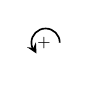
\begin{tikzpicture}[baseline=(char.base)]
    \node(char) at (0,0) {\(\scriptscriptstyle +\)};
    \draw[->, >=stealth, semithick] (0.2,0) arc (0:230:0.18cm);
  \end{tikzpicture}%
}

%====================================================================================
% Timer Ladder Symbol - Could be used for TON, TOF, RTO....
%====================================================================================
\tikzset{
    TON/.pic={

        \draw[
          BakerBlack
        ]
        (0,0)
        -- ++(0,0.375)
        -- ++(3.5,0)
        coordinate[pos=0.5](-TOP)
        -- ++(0,-1.75)
        coordinate[pos=3/14](-OUT)
        coordinate[pos=0.5](-EN1)
        coordinate[pos=0.875](-DN1)
        -- ++(-3.5,0)        
        -- (0,0)
        coordinate(-IN);

        \node[
          text=BakerBlack,
          font=\bfseries,
          anchor=east
        ](pre)
        at ($(-TOP)-(0,1.75em)$)
        {{\small PRE:}};

        \node[
          text=BakerBlack,
          font=\bfseries,
          anchor=east
        ](acc)
        at ($(pre.east)-(0,1em)$)
        {{\small ACC:}};

        \coordinate (-PRE) at (pre.east); % For the preset value
        \coordinate (-ACC) at (acc.east);

        \draw[
            BakerBlack
        ]
        (-EN1)
        -- ++(0.5,0)
        coordinate(-EN2)
        node[
            text=BakerBlack,
            anchor=west
        ]
        {{\small EN}};

        \draw[
            BakerBlack
        ]
        (-DN1)
        -- ++(0.5,0)
        coordinate(-DN2)
        node[
            text=BakerBlack,
            anchor=west
        ]
        {{\small DN}};

    }
}

%====================================================================================
% Oval ladder symbol, good for ONS, RES, etc.
%====================================================================================
\tikzset{
    ONS/.pic={

        \draw[
          BakerBlack
        ]
        (0,0)
        coordinate(-IN)
        -- ++(0.75,0)
        node[
          draw=BakerBlack, 
          text=BakerBlack, 
          font=\small, 
          minimum width=1.5cm, 
          minimum height=0.75cm, 
          anchor=west, 
          rounded corners=0.25cm
          ](ons){};
        
        \draw[BakerBlack] (ons.east) -- ++(0.75,0) coordinate(-OUT);

        \coordinate(-INS) at (ons.center);
        \coordinate(-VAR) at (ons.north); 
    }
}

%====================================================================================
% Source A, Source B, Dest box
%====================================================================================
\tikzset{
    SrcDest/.pic={
      
        \draw[
          BakerBlack
        ]
        (0,0)
        coordinate(-IN)
        -- ++(0,0.375)
        -- ++(5,0)
        coordinate[pos=0.5](-TOP)
        -- ++(0,-3.25)
        coordinate[pos=3/26](-OUT)
        -- ++(-5,0)
        -- (0,0)
        coordinate(l1);

        \node[
          text=BakerBlack,
          font=\bfseries,
          anchor=west
        ](srcA)
        at (l1)
        {{\small Src A:}};

        \node[
          text=BakerBlack,
          font=\bfseries,
          anchor=west
        ](srcB)
        at ($(l1)-(0,2em)$)
        {{\small Src B:}};

        \node[
          text=BakerBlack,
          font=\bfseries,
          anchor=west
        ](dest)
        at ($(srcB.west)-(0,2em)$)
        {{\small Dest:}};

        \coordinate(-SRCA) at (srcA.east);
        \coordinate(-AVAL) at ($(srcA.east)-(0,1em)$);
        \coordinate(-SRCB) at (srcB.east);
        \coordinate(-BVAL) at ($(srcB.east)-(0,1em)$);
        \coordinate(-DEST) at ($(-BVAL)-(0,1em)$);
        \coordinate(-DVAL) at ($(-DEST)-(0,1em)$);
    }
}

%====================================================================================
% Source A, Source B box
%====================================================================================
\tikzset{
    SrcAB/.pic={
      
        \draw[
          BakerBlack
        ]
        (0,0)
        coordinate(-IN)
        -- ++(0,0.375)
        -- ++(4,0)
        coordinate[pos=0.5](-TOP)
        -- ++(0,-2.25)
        coordinate[pos=1/6](-OUT)
        -- ++(-4,0)
        -- (0,0)
        coordinate(l1);

        \node[
          text=BakerBlack,
          font=\bfseries,
          anchor=west
        ](srcA)
        at (l1)
        {{\small Src A:}};

        \node[
          text=BakerBlack,
          font=\bfseries,
          anchor=west
        ](srcB)
        at ($(l1)-(0,2em)$)
        {{\small Src B:}};

        \coordinate(-SRCA) at (srcA.east);
        \coordinate(-AVAL) at ($(srcA.east)-(0,1em)$);
        \coordinate(-SRCB) at (srcB.east);
        \coordinate(-BVAL) at ($(srcB.east)-(0,1em)$);
    }
}

%====================================================================================
% LIMIT instruction
%====================================================================================
\tikzset{
    Limit/.pic={
      
        \draw[
          BakerBlack
        ]
        (0,0)
        coordinate(-IN)
        -- ++(0,0.375)
        -- ++(4,0)
        coordinate[pos=0.5](-TOP)
        -- ++(0,-3.25)
        coordinate[pos=3/26](-OUT)
        -- ++(-4,0)
        -- (0,0)
        coordinate(l1);

        \node[
          text=BakerBlack,
          font=\bfseries,
          anchor=west
        ](srcA)
        at (l1)
        {{\small Low:}};

        \node[
          text=BakerBlack,
          font=\bfseries,
          anchor=west
        ](srcB)
        at ($(l1)-(0,2em)$)
        {{\small Test:}};

        \node[
          text=BakerBlack,
          font=\bfseries,
          anchor=west
        ](dest)
        at ($(srcB.west)-(0,2em)$)
        {{\small High:}};

        \coordinate(-LO) at (srcA.east);
        \coordinate(-LOV) at ($(srcA.east)-(0,1em)$);
        \coordinate(-TEST) at (srcB.east);
        \coordinate(-TESTV) at ($(srcB.east)-(0,1em)$);
        \coordinate(-HI) at ($(-TESTV)-(0,1em)$);
        \coordinate(-HIV) at ($(-HI)-(0,1em)$);
    }
}

%====================================================================================
% Source Destination box
%====================================================================================
\tikzset{
    SrcSingle/.pic={
      
        \draw[
          BakerBlack
        ]
        (0,0)
        coordinate(-IN)
        -- ++(0,0.375)
        -- ++(6,0)
        coordinate[pos=0.5](-TOP)
        -- ++(0,-2.25)
        coordinate[pos=1/6](-OUT)
        -- ++(-6,0)
        -- (0,0)
        coordinate(l1);

        \node[
          text=BakerBlack,
          font=\bfseries,
          anchor=west
        ](srcA)
        at (l1)
        {{\small Source:}};

        \node[
          text=BakerBlack,
          font=\bfseries,
          anchor=east
        ](srcB)
        at ($(srcA.east)-(0,2em)$)
        {{\small Dest:}};

        \coordinate(-SRC) at (srcA.east);
        \coordinate(-SRCV) at ($(srcA.east)-(0,1em)$);
        \coordinate(-DEST) at (srcB.east);
        \coordinate(-DESTV) at ($(srcB.east)-(0,1em)$);
    }
}

%====================================================================================
% Compute Box
%====================================================================================
\tikzset{
    CPT/.pic={
      
        \draw[
          BakerBlack
        ]
        (0,0)
        coordinate(-IN)
        -- ++(0,0.375)
        -- ++(8.5,0)
        coordinate[pos=0.5](-TOP)
        -- ++(0,-1.75)
        coordinate[pos=3/14](-OUT)
        -- ++(-8.5,0)
        -- (0,0)
        coordinate(l1);

        \node[
          text=BakerBlack,
          font=\bfseries,
          anchor=west
        ](srcA)
        at (l1)
        {{\small Source:}};

        \node[
          text=BakerBlack,
          font=\bfseries,
          anchor=east
        ](srcB)
        at ($(srcA.east)-(0,2em)$)
        {{\small Exp:}};

        \coordinate(-DEST) at (srcA.east);
        \coordinate(-DESTV) at ($(srcA.east)-(0,1em)$);
        \coordinate(-EXP) at (srcB.east);
        \coordinate(-EXPV) at ($(srcB.east)-(0,1em)$);
    }
}

% ============================================================================
% Document Content
% ============================================================================
\begin{document}

\maketitle              % Redefined in the preamble to generate a full frame

\begin{frame}
    \frametitle{Agenda}
    \begingroup
        % Tighten the spacing between paragraphs/TOC lines
        \setlength{\parskip}{0.3em} 
        
        % Optionally tighten the line spacing within an entry
        %\baselineskip=1.2em 
        
        \setcounter{tocdepth}{1} % Show only sections
    \tableofcontents
    \setcounter{tocdepth}{2} % Reset back to default so subsections are tracked
    \endgroup
\end{frame}

\section{Material Principles}

\subsection{Properties of Steel}

\begin{frame}
	\frametitle{Strength}

    \begin{columns}
        \begin{column}{0.48\linewidth}
            \begin{itemize}[<+- | alert@+>]
                \item The ability of a material to withstand tensile, compressive, or shear loading without deformation or failing
            \end{itemize}
        \end{column}
        \begin{column}{0.48\linewidth}
            \shadowpic[]{0.75\linewidth}{A technical line diagram illustrating the five stages of ductile fracture in a cylindrical tensile specimen against a white background, starting on the left with a vertical cylinder narrowed in the middle labeled Necking, which zooms into a sequence of four dashed circular detail views connected by arrows showing Void Nucleation with three small green voids inside the neck, Void Coalescence where the voids merge into a single elongated green cavity, Crack Propagation with thin diagonal cracks extending from the cavity tips, and Separation where the specimen fractures completely into two jagged cup-and-cone pieces.}{\textbf{Attribution:} \href{https://commons.wikimedia.org/wiki/File:Ductile_fracture_upd.png}{Bbanerje at English Wikipedia}, \href{http://creativecommons.org/licenses/by-sa/3.0/}{CC BY-SA 3.0}, via Wikimedia Commons}{Ductile_fracture_upd}
        \end{column}
    \end{columns}
\end{frame}

\begin{frame}
	\frametitle{Toughness}

    \begin{columns}
        \begin{column}{0.48\linewidth}
            \begin{itemize}[<+- | alert@+>]
                \item The ability of a material to withstand impact or shock loading without fracturing
            \end{itemize}
        \end{column}
        \begin{column}{0.48\linewidth}
            \shadowpic[]{0.75\linewidth}{A stroboscopic time-lapse photograph against a solid black background showing a yellow basketball bouncing across the frame from left to right along two consecutive parabolic arcs, with the ball positions spaced wider apart during faster vertical movement near the bottom and overlapping closely near the slower peak of each bounce as the second arc reaches a lower maximum height than the first.}{\textbf{Attribution:} \href{https://commons.wikimedia.org/wiki/File:Bouncing_ball_strobe_edit.jpg}{MichaelMaggs Edit by Richard Bartz}, \href{http://creativecommons.org/licenses/by-sa/3.0/}{CC BY-SA 3.0}, via Wikimedia Commons}{Bouncing_ball_strobe_edit}
        \end{column}
    \end{columns}
\end{frame}

\begin{frame}
	\frametitle{Hardness}

    \begin{columns}
        \begin{column}{0.48\linewidth}
            \begin{itemize}[<+- | alert@+>]
                \item The ability of a material to withstand deformation, scratching, or other surface damage
            \end{itemize}
        \end{column}
        \begin{column}{0.48\linewidth}
            \shadowpic[]{0.75\linewidth}{A close-up macro photograph of several round brilliant-cut diamonds scattered on a bright white surface, featuring one large sharply focused diamond in the center displaying intricate internal facets and light reflections, surrounded by smaller out-of-focus diamonds resting both face-up and on their sides with soft shadows.}{\textbf{Attribution:} \href{https://commons.wikimedia.org/wiki/File:Brillanten.jpg}{Mario Sarto}, \href{http://creativecommons.org/licenses/by-sa/3.0/}{CC BY-SA 3.0}, via Wikimedia Commons}{Brillanten}
        \end{column}
    \end{columns}
\end{frame}

\begin{frame}
	\frametitle{Strength, Toughness, and Hardness}

    \begin{columns}
        \begin{column}{0.48\linewidth}
            \begin{itemize}[<+- | alert@+>]
                \item{Strength and toughness usually go together}
                \item{Inverse proportion to hardness}
                    \begin{itemize}
                        \item{As steel becomes hard it becomes \emph{brittle}}
                        \item{Very hard steel will shatter like glass--very low strength/toughness}
                    \end{itemize}
            \end{itemize}
        \end{column}
        \begin{column}{0.48\linewidth}
            \shadowpic[]{0.75\linewidth}{A rusted and severely bent structural steel beam from the World Trade Center on display inside a low-railing exhibit at the National September 11 Memorial and Museum, folded sharply back upon itself in a tight U-shaped curve against a stained concrete slurry wall featuring recessed square niches.}{\textbf{Attribution:} \href{https://commons.wikimedia.org/wiki/File:2016_9-11_Museum_broken_steel.jpg}{Beyond My Ken}, \href{http://creativecommons.org/licenses/by-sa/4.0/}{CC BY-SA 4.0}, via Wikimedia Commons}{2016_9-11_Museum_broken_steel}
        \end{column}
    \end{columns}
\end{frame}

\subsection{Composition of Steel}

\begin{frame}
	\frametitle{Primary Elements of Steel}

    \begin{columns}
        \begin{column}{0.48\linewidth}
            \begin{itemize}[<+- | alert@+>]
                \item Steel is a \emph{chemical mixture} of multiple elements
                \item{Carbon steel = iron + carbon}
                    \begin{itemize}
                        \item Low carbon steel <0.2\% carbon
                        \item High carbon steel >0.5\% carbon
                    \end{itemize}
            \end{itemize}
        \end{column}
        \begin{column}{0.48\linewidth}
            \shadowpic[]{\linewidth}{A row of cylindrical metal bars of varying diameters arranged side by side on a glossy dark surface that reflects their shiny machined end faces against a gray background, progressing from larger round bars on the left to smaller round and square bars on the right.}{\textbf{Attribution:} \href{https://commons.wikimedia.org/wiki/File:Stainless_Steel_Carbon_Steel_Mild_Steel_Duplex_Steel_nickel_Alloys_Titanium_CuproNickel_Round_Bar.jpg}{Jatinsanghvi}, \href{http://creativecommons.org/licenses/by-sa/3.0/}{CC BY-SA 3.0}, via Wikimedia Commons}{Stainless_Steel_Carbon_Steel_Mild_Steel_Duplex_Steel_nickel_Alloys_Titanium_CuproNickel_Round_Bar}
        \end{column}
    \end{columns}
\end{frame}

\begin{frame}
	\frametitle{Alloy Elements (1 of 2)}

    \begin{columns}
        \begin{column}{0.48\linewidth}
            \begin{itemize}[<+- | alert@+>]
                \item Other \emph{alloying} elements can be added for specific properties
            \end{itemize}
        \end{column}
        \begin{column}{0.48\linewidth}
            \shadowpic[]{\linewidth}{A row of cylindrical metal bars of varying diameters arranged side by side on a glossy dark surface that reflects their shiny machined end faces against a gray background, progressing from larger round bars on the left to smaller round and square bars on the right.}{\textbf{Attribution:} \href{https://commons.wikimedia.org/wiki/File:Stainless_Steel_Carbon_Steel_Mild_Steel_Duplex_Steel_nickel_Alloys_Titanium_CuproNickel_Round_Bar.jpg}{Jatinsanghvi}, \href{http://creativecommons.org/licenses/by-sa/3.0/}{CC BY-SA 3.0}, via Wikimedia Commons}{Stainless_Steel_Carbon_Steel_Mild_Steel_Duplex_Steel_nickel_Alloys_Titanium_CuproNickel_Round_Bar}
        \end{column}
    \end{columns}
\end{frame}

\begin{frame}
	\frametitle{Alloy Elements (2 of 2)}

    \begin{columns}
        \begin{column}{0.48\linewidth}
            \begin{description}[<+- | alert@+>]
                \item[Manganese] decrease brittleness, increase strength
                \item[Phosphorous] increase strength/corrosion resistance
                \item[Sulphur] improves machinability
            \end{description}
        \end{column}
        \begin{column}{0.48\linewidth}
            \shadowpic[]{\linewidth}{A row of cylindrical metal bars of varying diameters arranged side by side on a glossy dark surface that reflects their shiny machined end faces against a gray background, progressing from larger round bars on the left to smaller round and square bars on the right.}{\textbf{Attribution:} \href{https://commons.wikimedia.org/wiki/File:Stainless_Steel_Carbon_Steel_Mild_Steel_Duplex_Steel_nickel_Alloys_Titanium_CuproNickel_Round_Bar.jpg}{Jatinsanghvi}, \href{http://creativecommons.org/licenses/by-sa/3.0/}{CC BY-SA 3.0}, via Wikimedia Commons}{Stainless_Steel_Carbon_Steel_Mild_Steel_Duplex_Steel_nickel_Alloys_Titanium_CuproNickel_Round_Bar}
        \end{column}
    \end{columns}
\end{frame}

\begin{frame}
	\frametitle{AISI Steel Designations}

    \begin{columns}
        \begin{column}{0.48\linewidth}
            \begin{itemize}[<+- | alert@+>]
                \item 4 digit designation for steel
                    \begin{itemize}
                        \item First 2: main alloy elements
                        \item Second 2: carbon content
                    \end{itemize}
            \end{itemize}
        \end{column}
        \begin{column}{0.48\linewidth}
            \shadowpic[]{\linewidth}{A row of cylindrical metal bars of varying diameters arranged side by side on a glossy dark surface that reflects their shiny machined end faces against a gray background, progressing from larger round bars on the left to smaller round and square bars on the right.}{\textbf{Attribution:} \href{https://commons.wikimedia.org/wiki/File:Stainless_Steel_Carbon_Steel_Mild_Steel_Duplex_Steel_nickel_Alloys_Titanium_CuproNickel_Round_Bar.jpg}{Jatinsanghvi}, \href{http://creativecommons.org/licenses/by-sa/3.0/}{CC BY-SA 3.0}, via Wikimedia Commons}{Stainless_Steel_Carbon_Steel_Mild_Steel_Duplex_Steel_nickel_Alloys_Titanium_CuproNickel_Round_Bar}
        \end{column}
    \end{columns}
\end{frame}

\begin{frame}
	\frametitle{Example: 1018 Steel}

    \begin{columns}[t]
        \begin{column}{0.48\linewidth}
            \begin{itemize}[<+- | alert@+>]
                \item General use--easy to machine/weld/heat treat
            \end{itemize}
        \end{column}
        \begin{column}{0.48\linewidth}
            \begin{description}
                \item[Carbon] 0.14-0.20\%
                \item[Manganese] 0.60-0.90\%
                \item[Phosphorous] $\leq$0.040\%
                \item[Sulphur] $\leq$0.050\%
            \end{description}
        \end{column}
    \end{columns}
\end{frame}

\begin{frame}
	\frametitle{Example: 1045 Steel}

    \begin{columns}[t]
        \begin{column}{0.48\linewidth}
            \begin{itemize}[<+- | alert@+>]
                \item Higher strength/impact resistance
                \item Not as easy to weld
                \item fewer heat treat options
            \end{itemize}
        \end{column}
        \begin{column}{0.48\linewidth}
            \begin{description}
                \item[Carbon] 0.43-0.50\%
                \item[Manganese] 0.60-0.90\%
                \item[Phosphorous] $\leq$0.040\%
                \item[Sulphur] $\leq$0.050\%
            \end{description}
        \end{column}
    \end{columns}
\end{frame}

\begin{frame}
	\frametitle{Example: 4140 Steel (1 of 2)}

    \begin{columns}[t]
        \begin{column}{0.48\linewidth}
            \begin{itemize}[<+- | alert@+>]
                \item 41XX = Chromium/Molybdenum
            \end{itemize}
        \end{column}
        \begin{column}{0.48\linewidth}
            \begin{description}[<+- | alert@+>]
                \item[Chromium] hardness penetration
                \item[Molybdenum] uniform hardness
            \end{description}
        \end{column}
    \end{columns}
\end{frame}

\begin{frame}
	\frametitle{Example: 4140 Steel (2 of 2)}

    \begin{columns}[t]
        \begin{column}{0.48\linewidth}
            \begin{itemize}[<+- | alert@+>]
                \item Easy to machine
                \item Hard to weld
                \item Easy to harden
            \end{itemize}
        \end{column}
        \begin{column}{0.48\linewidth}
            \begin{description}
                \item[Carbon] 0.38-0.43\%
                \item[Chromium] 0.80-1.10\%
                \item[Molybdenum] 0.15-0.25\%
                \item[Manganese] 0.75-1.0\%
                \item[Phosphorous] $\leq$0.035\%
                \item[Sulphur] $\leq$0.040\%
            \end{description}
        \end{column}
    \end{columns}
\end{frame}

\subsection{Constituents of Steel}

\begin{frame}
	\frametitle{Constituents of Steel}

    \begin{columns}[t]
        \begin{column}{0.48\linewidth}
            \begin{itemize}[<+- | alert@+>]
                \item Atoms in iron and steel form structures known as \emph{constituents}
                \item Constiuents are basically the arrangement of iron and carbon crystals within the steel
            \end{itemize}
        \end{column}
        \begin{column}{0.48\linewidth}
            \begin{enumerate}[<+- | alert@+>]
                \item Ferrite
                \item Cementite
                \item Pearlite
                \item Martensite
                \item Austenite
            \end{enumerate}
        \end{column}
    \end{columns}
\end{frame}

\begin{frame}
	\frametitle{Ferrite}

    \begin{columns}
        \begin{column}{0.48\linewidth}
            \begin{itemize}[<+- | alert@+>]
                \item Almost pure iron
                \item Soft and ductile
                \item Called the alpha (\alpha{}) phase
                \item Does not harden when quenched, but crystals get smaller
            \end{itemize}
        \end{column}
        \begin{column}{0.48\linewidth}
            \shadowpic[]{\linewidth}{A grayscale optical micrograph of ASTM A285 carbon steel showing a two-phase ferrite and pearlite microstructure, consisting of interlocking light gray polygonal and elongated ferrite grains interspersed with irregular dark black pearlite colonies, with a white 100 micrometer scale bar in the lower right corner.}{\textbf{Attribution:} \href{https://commons.wikimedia.org/wiki/File:Ferrite-perlite-steel-A285.jpeg}{A. J. Duncan, K. H. Subramanian, R. L. Sindelar, K. Miller, A. P. Reynolds, and Y. J. Chao}, Public domain, via Wikimedia Commons}{Ferrite-perlite-steel-A285}

            \centering
            \vspace{0.5em}
            {\footnotesize The ferrite is gray in this micrograph.\par}
        \end{column}
    \end{columns}
\end{frame}

\begin{frame}
	\frametitle{Cementite}

    \begin{columns}
        \begin{column}{0.48\linewidth}
            \begin{itemize}[<+- | alert@+>]
                \item $Fe_3C$ molecule
                \item Extremely hard--harder than steel or glass
                \item Increases with \% carbon
                \item Contains 6.6\% carbon
                \item Decreases tensile strength of steel, increases hardness and machinability
            \end{itemize}
        \end{column}
        \begin{column}{0.48\linewidth}
            \shadowpic[]{\linewidth}{A grayscale optical micrograph of ASTM A285 carbon steel showing a two-phase ferrite and pearlite microstructure, consisting of interlocking light gray polygonal and elongated ferrite grains interspersed with irregular dark black pearlite colonies, with a white 100 micrometer scale bar in the lower right corner.}{\textbf{Attribution:} \href{https://commons.wikimedia.org/wiki/File:Ferrite-perlite-steel-A285.jpeg}{A. J. Duncan, K. H. Subramanian, R. L. Sindelar, K. Miller, A. P. Reynolds, and Y. J. Chao}, Public domain, via Wikimedia Commons}{Ferrite-perlite-steel-A285}

            \centering
            \vspace{0.5em}
            {\footnotesize The cementite is black in this micrograph.\par}
        \end{column}
    \end{columns}
\end{frame}

\begin{frame}
	\frametitle{Pearlite (1 of 2)}

    \begin{columns}
        \begin{column}{0.48\linewidth}
            \begin{itemize}[<+- | alert@+>]
                \item A mixture of 87.5\% ferrite and 12.5\% cementite
                \item Alternating layers of ferrite and cementite
                    \begin{itemize}
                        \item Looks like a pearl--pearlite
                    \end{itemize}
                \item Rate of cooling determines thickness and distance between plates
            \end{itemize}
        \end{column}
        \begin{column}{0.48\linewidth}
            \shadowpic[]{\linewidth}{A scanning electron micrograph showing the lamellar microstructure of pearlite in steel, featuring densely packed parallel alternating layers of bright white cementite plates and darker gray ferrite bands arranged in differently oriented colonies, separated by smooth dark ferrite regions, with a black data bar at the bottom left displaying a 5 micrometer scale bar at 2000 times magnification.}{\textbf{Attribution:} \href{https://commons.wikimedia.org/wiki/File:Pearlite.jpg}{Michelshock}, Public domain, via Wikimedia Commons}{Pearlite}
        \end{column}
    \end{columns}
\end{frame}

\begin{frame}
	\frametitle{Pearlite (2 of 2)}
    \begin{columns}
        \begin{column}{0.48\linewidth}
            \begin{itemize}[<+- | alert@+>]
                \item 0\% in pure iron
                \item 100\% in 0.9\% carbon steel
                \item Soft steel = mixture of ferrite and pearlite
                \item Hardness increases with proportion of pearlite
                \item Hard steel = mixture of pearlite and cementite
            \end{itemize}
        \end{column}
        \begin{column}{0.48\linewidth}
            \shadowpic[]{\linewidth}{A scanning electron micrograph showing the lamellar microstructure of pearlite in steel, featuring densely packed parallel alternating layers of bright white cementite plates and darker gray ferrite bands arranged in differently oriented colonies, separated by smooth dark ferrite regions, with a black data bar at the bottom left displaying a 5 micrometer scale bar at 2000 times magnification.}{\textbf{Attribution:} \href{https://commons.wikimedia.org/wiki/File:Pearlite.jpg}{Michelshock}, Public domain, via Wikimedia Commons}{Pearlite}
        \end{column}
    \end{columns}
\end{frame}

\begin{frame}
	\frametitle{Martensite}

    \begin{columns}
        \begin{column}{0.48\linewidth}
            \begin{itemize}[<+- | alert@+>]
                \item Hard, brittle mass of fibrous/needle like structures
                \item Chief component of hardened steel
                \item Formed by rapid quenching of steel above critical temperature
                \item Not as tough as austenite
                \item Magnetic
            \end{itemize}
        \end{column}
        \begin{column}{0.48\linewidth}
            \shadowpic[]{\linewidth}{An optical micrograph of tempered martensite in steel, displaying a dense, fine-grained matrix of dark intersecting needle-like laths interspersed with small bright white patches, with a dark reddish-brown 50 micrometer scale bar in the lower right corner.}{\textbf{Attribution:} \href{https://commons.wikimedia.org/wiki/File:20180308_Martensite_rinvenuta.jpg}{Melancholia\textasciitilde{}itwiki}, \href{http://creativecommons.org/licenses/by-sa/4.0/}{CC BY-SA 4.0}, via Wikimedia Commons}{Pearlite}
        \end{column}
    \end{columns}
\end{frame}

\begin{frame}
	\frametitle{Austenite (1 of 2)}

    \begin{columns}
        \begin{column}{0.48\linewidth}
            \begin{itemize}[<+- | alert@+>]
                \item Only exists within a particular range of temperature
                \item Forms when >1.1\% carbon steel is quenched from \qty{1,000}{\degreeCelsius}
                \item Below \qty{700}{\degreeCelsius} transforms into pearlite, ferrite, cementite
            \end{itemize}
        \end{column}
        \begin{column}{0.48\linewidth}
            \shadowpic[]{\linewidth}{An optical micrograph showing the austenitic grain structure of AISI 304 stainless steel against a pale golden-brown background, featuring interlocking polygonal crystal grains defined by dark grain boundaries, straight parallel annealing twin bands across several grains, scattered small dark inclusion dots, and a 100 micrometer scale bar in the upper left corner.}{\textbf{Attribution:} \href{https://commons.wikimedia.org/wiki/File:AISI_304_-_austenitic_structure.jpg}{Melancholia\textasciitilde{}itwiki}, \href{http://creativecommons.org/licenses/by-sa/4.0/}{CC BY-SA 4.0}, via Wikimedia Commons}{AISI_304_-_austenitic_structure}
        \end{column}
    \end{columns}
\end{frame}

\begin{frame}
	\frametitle{Austenite (2 of 2)}

    \begin{columns}
        \begin{column}{0.48\linewidth}
            \begin{itemize}[<+- | alert@+>]
                \item Austenitic steels require special heat treatment
                \item Non-magnetic
            \end{itemize}
        \end{column}
        \begin{column}{0.48\linewidth}
            \shadowpic[]{\linewidth}{An optical micrograph showing the austenitic grain structure of AISI 304 stainless steel against a pale golden-brown background, featuring interlocking polygonal crystal grains defined by dark grain boundaries, straight parallel annealing twin bands across several grains, scattered small dark inclusion dots, and a 100 micrometer scale bar in the upper left corner.}{\textbf{Attribution:} \href{https://commons.wikimedia.org/wiki/File:AISI_304_-_austenitic_structure.jpg}{Melancholia\textasciitilde{}itwiki}, \href{http://creativecommons.org/licenses/by-sa/4.0/}{CC BY-SA 4.0}, via Wikimedia Commons}{AISI_304_-_austenitic_structure}
        \end{column}
    \end{columns}
\end{frame}

\subsection{Heat Treatment}

\begin{frame}
    \frametitle{Phase Diagrams}

    \begin{figure}
        \centering
        \resizebox{0.5\linewidth}{!}{
            % <a href="https://commons.wikimedia.org/wiki/File:Iron_carbon_phase_diagram.svg">AG Caesar</a>, <a href="https://creativecommons.org/licenses/by-sa/4.0">CC BY-SA 4.0</a>, via Wikimedia Commons
\begin{tikzpicture}[
    american, 
    >={Latex[length=5mm, width=2mm]},
    alt={}
    ]

    
  \path[draw=BakerBlack,line cap=,line width=0.5cm,miter limit=10.0] (17.8, -130.2)
   -- (17.8, -7.1);



  \path[fill=BakerBlack] (17.8, -4.1) -- (19.5, -8.3) -- (17.8, -7.3) -- (16.0, 
  -8.3) -- (17.8, -4.1)-- cycle;;



  \path[draw=BakerBlack,line cap=,line width=0.5cm,miter limit=10.0] (17.8, -130.2)
   -- (196.6, -130.2);



  \path[fill=BakerBlack] (199.5, -130.2) -- (195.3, -131.9) -- (196.3, -130.2) -- 
  (195.3, -128.5) -- (199.5, -130.2)-- cycle;;



  \path[draw=BakerBlack,line cap=,line width=0.4cm,miter limit=10.0] (15.5, -116.7)
   -- (17.8, -116.7);



  \path[draw=BakerBlack,line cap=,line width=0.4cm,miter limit=10.0] (15.5, -101.7)
   -- (17.8, -101.7);



  \path[draw=BakerBlack,line cap=,line width=0.4cm,miter limit=10.0] (15.5, -86.7) 
  -- (17.8, -86.7);



  \path[draw=BakerBlack,line cap=,line width=0.4cm,miter limit=10.0] (15.5, -71.7) 
  -- (17.8, -71.7);



  \path[draw=BakerBlack,line cap=,line width=0.4cm,miter limit=10.0] (15.5, -56.7) 
  -- (17.8, -56.7);



  \path[draw=BakerBlack,line cap=,line width=0.4cm,miter limit=10.0] (15.5, -41.7) 
  -- (17.8, -41.7);



  \path[draw=BakerBlack,line cap=,line width=0.4cm,miter limit=10.0] (15.5, -26.7) 
  -- (17.8, -26.7);



  \path[draw=BakerBlack,line cap=,line width=0.4cm,miter limit=10.0] (15.5, -11.7) 
  -- (17.8, -11.7);



  \path[draw=BakerBlack,line cap=,line width=0.4cm,miter limit=10.0] (69.1, -132.5)
   -- (69.1, -130.2);



  \path[draw=BakerBlack,line cap=,line width=0.4cm,miter limit=10.0] (171.9, 
  -130.2) -- (171.9, -132.5);



  \path[draw=BakerBlack,line cap=,line width=0.4cm,miter limit=10.0] (120.5, 
  -130.2) -- (120.5, -132.5);



  \path[fill] (10.9, -117.4) -- (10.7, -117.8) -- (9.5, -117.8) -- (9.5, 
  -117.7).. controls (9.9, -117.4) and (10.1, -117.1) .. (10.3, -116.9).. 
  controls (10.4, -116.7) and (10.5, -116.5) .. (10.5, -116.3).. controls (10.5,
   -116.2) and (10.5, -116.1) .. (10.4, -116.0).. controls (10.3, -115.9) and 
  (10.2, -115.9) .. (10.1, -115.9).. controls (10.0, -115.9) and (9.9, -115.9) 
  .. (9.8, -116.0).. controls (9.7, -116.0) and (9.7, -116.1) .. (9.6, -116.2) 
  -- (9.6, -116.2).. controls (9.6, -116.0) and (9.7, -115.9) .. (9.8, -115.8)..
   controls (9.9, -115.7) and (10.0, -115.6) .. (10.2, -115.6).. controls (10.3,
   -115.6) and (10.5, -115.7) .. (10.6, -115.8).. controls (10.7, -115.9) and 
  (10.8, -116.0) .. (10.8, -116.2).. controls (10.8, -116.3) and (10.7, -116.4) 
  .. (10.7, -116.5).. controls (10.6, -116.7) and (10.5, -116.8) .. (10.3, 
  -117.0).. controls (10.1, -117.3) and (9.9, -117.5) .. (9.8, -117.5) -- (10.4,
   -117.5).. controls (10.5, -117.5) and (10.6, -117.5) .. (10.6, -117.5).. 
  controls (10.7, -117.5) and (10.7, -117.5) .. (10.7, -117.5).. controls (10.8,
   -117.4) and (10.8, -117.4) .. (10.8, -117.4) -- (10.9, -117.4) -- (10.9, 
  -117.4) -- cycle;



  \path[fill] (11.1, -116.7).. controls (11.1, -116.5) and (11.2, -116.3) .. 
  (11.2, -116.1).. controls (11.3, -115.9) and (11.4, -115.8) .. (11.5, 
  -115.7).. controls (11.6, -115.7) and (11.7, -115.6) .. (11.8, -115.6).. 
  controls (12.0, -115.6) and (12.1, -115.7) .. (12.3, -115.9).. controls (12.4,
   -116.1) and (12.5, -116.4) .. (12.5, -116.7).. controls (12.5, -116.9) and 
  (12.5, -117.2) .. (12.4, -117.3).. controls (12.3, -117.5) and (12.2, -117.6) 
  .. (12.1, -117.7).. controls (12.0, -117.8) and (11.9, -117.8) .. (11.8, 
  -117.8).. controls (11.6, -117.8) and (11.4, -117.7) .. (11.3, -117.5).. 
  controls (11.2, -117.3) and (11.1, -117.0) .. (11.1, -116.7) -- cycle(11.4, 
  -116.8).. controls (11.4, -117.1) and (11.5, -117.3) .. (11.5, -117.5).. 
  controls (11.6, -117.6) and (11.7, -117.7) .. (11.8, -117.7).. controls (11.9,
   -117.7) and (11.9, -117.7) .. (12.0, -117.6).. controls (12.0, -117.6) and 
  (12.1, -117.5) .. (12.1, -117.4).. controls (12.2, -117.2) and (12.2, -117.0) 
  .. (12.2, -116.6).. controls (12.2, -116.4) and (12.2, -116.2) .. (12.1, 
  -116.0).. controls (12.1, -115.9) and (12.0, -115.8) .. (12.0, -115.8).. 
  controls (11.9, -115.7) and (11.9, -115.7) .. (11.8, -115.7).. controls (11.8,
   -115.7) and (11.7, -115.8) .. (11.6, -115.8).. controls (11.6, -115.9) and 
  (11.5, -116.0) .. (11.5, -116.2).. controls (11.5, -116.4) and (11.4, -116.6) 
  .. (11.4, -116.8) -- cycle;



  \path[fill] (12.7, -116.7).. controls (12.7, -116.5) and (12.8, -116.3) .. 
  (12.8, -116.1).. controls (12.9, -115.9) and (13.0, -115.8) .. (13.1, 
  -115.7).. controls (13.2, -115.7) and (13.3, -115.6) .. (13.4, -115.6).. 
  controls (13.6, -115.6) and (13.7, -115.7) .. (13.8, -115.9).. controls (14.0,
   -116.1) and (14.1, -116.4) .. (14.1, -116.7).. controls (14.1, -116.9) and 
  (14.1, -117.2) .. (14.0, -117.3).. controls (13.9, -117.5) and (13.8, -117.6) 
  .. (13.7, -117.7).. controls (13.6, -117.8) and (13.5, -117.8) .. (13.4, 
  -117.8).. controls (13.2, -117.8) and (13.0, -117.7) .. (12.9, -117.5).. 
  controls (12.8, -117.3) and (12.7, -117.0) .. (12.7, -116.7) -- cycle(13.0, 
  -116.8).. controls (13.0, -117.1) and (13.1, -117.3) .. (13.1, -117.5).. 
  controls (13.2, -117.6) and (13.3, -117.7) .. (13.4, -117.7).. controls (13.5,
   -117.7) and (13.5, -117.7) .. (13.6, -117.6).. controls (13.6, -117.6) and 
  (13.7, -117.5) .. (13.7, -117.4).. controls (13.8, -117.2) and (13.8, -117.0) 
  .. (13.8, -116.6).. controls (13.8, -116.4) and (13.8, -116.2) .. (13.7, 
  -116.0).. controls (13.7, -115.9) and (13.6, -115.8) .. (13.6, -115.8).. 
  controls (13.5, -115.7) and (13.5, -115.7) .. (13.4, -115.7).. controls (13.3,
   -115.7) and (13.3, -115.8) .. (13.2, -115.8).. controls (13.2, -115.9) and 
  (13.1, -116.0) .. (13.1, -116.2).. controls (13.0, -116.4) and (13.0, -116.6) 
  .. (13.0, -116.8) -- cycle;



  \path[fill] (10.9, -102.0) -- (10.9, -102.2) -- (10.6, -102.2) -- (10.6, 
  -102.8) -- (10.4, -102.8) -- (10.4, -102.2) -- (9.5, -102.2) -- (9.5, -102.0) 
  -- (10.5, -100.6) -- (10.6, -100.6) -- (10.6, -102.0) -- (10.9, -102.0) -- 
  cycle(10.4, -102.0) -- (10.4, -101.0) -- (9.6, -102.0) -- (10.4, -102.0) -- 
  cycle;



  \path[fill] (11.1, -101.7).. controls (11.1, -101.5) and (11.2, -101.3) .. 
  (11.2, -101.1).. controls (11.3, -100.9) and (11.4, -100.8) .. (11.5, 
  -100.7).. controls (11.6, -100.7) and (11.7, -100.6) .. (11.8, -100.6).. 
  controls (12.0, -100.6) and (12.1, -100.7) .. (12.3, -100.9).. controls (12.4,
   -101.1) and (12.5, -101.4) .. (12.5, -101.7).. controls (12.5, -101.9) and 
  (12.5, -102.2) .. (12.4, -102.3).. controls (12.3, -102.5) and (12.2, -102.6) 
  .. (12.1, -102.7).. controls (12.0, -102.8) and (11.9, -102.8) .. (11.8, 
  -102.8).. controls (11.6, -102.8) and (11.4, -102.7) .. (11.3, -102.5).. 
  controls (11.2, -102.3) and (11.1, -102.0) .. (11.1, -101.7) -- cycle(11.4, 
  -101.8).. controls (11.4, -102.1) and (11.5, -102.3) .. (11.5, -102.5).. 
  controls (11.6, -102.6) and (11.7, -102.7) .. (11.8, -102.7).. controls (11.9,
   -102.7) and (11.9, -102.7) .. (12.0, -102.6).. controls (12.0, -102.6) and 
  (12.1, -102.5) .. (12.1, -102.4).. controls (12.2, -102.2) and (12.2, -102.0) 
  .. (12.2, -101.6).. controls (12.2, -101.4) and (12.2, -101.2) .. (12.1, 
  -101.0).. controls (12.1, -100.9) and (12.0, -100.8) .. (12.0, -100.8).. 
  controls (11.9, -100.7) and (11.9, -100.7) .. (11.8, -100.7).. controls (11.8,
   -100.7) and (11.7, -100.8) .. (11.6, -100.8).. controls (11.6, -100.9) and 
  (11.5, -101.0) .. (11.5, -101.2).. controls (11.5, -101.4) and (11.4, -101.6) 
  .. (11.4, -101.8) -- cycle;



  \path[fill] (12.7, -101.7).. controls (12.7, -101.5) and (12.8, -101.3) .. 
  (12.8, -101.1).. controls (12.9, -100.9) and (13.0, -100.8) .. (13.1, 
  -100.7).. controls (13.2, -100.7) and (13.3, -100.6) .. (13.4, -100.6).. 
  controls (13.6, -100.6) and (13.7, -100.7) .. (13.8, -100.9).. controls (14.0,
   -101.1) and (14.1, -101.4) .. (14.1, -101.7).. controls (14.1, -101.9) and 
  (14.1, -102.2) .. (14.0, -102.3).. controls (13.9, -102.5) and (13.8, -102.6) 
  .. (13.7, -102.7).. controls (13.6, -102.8) and (13.5, -102.8) .. (13.4, 
  -102.8).. controls (13.2, -102.8) and (13.0, -102.7) .. (12.9, -102.5).. 
  controls (12.8, -102.3) and (12.7, -102.0) .. (12.7, -101.7) -- cycle(13.0, 
  -101.8).. controls (13.0, -102.1) and (13.1, -102.3) .. (13.1, -102.5).. 
  controls (13.2, -102.6) and (13.3, -102.7) .. (13.4, -102.7).. controls (13.5,
   -102.7) and (13.5, -102.7) .. (13.6, -102.6).. controls (13.6, -102.6) and 
  (13.7, -102.5) .. (13.7, -102.4).. controls (13.8, -102.2) and (13.8, -102.0) 
  .. (13.8, -101.6).. controls (13.8, -101.4) and (13.8, -101.2) .. (13.7, 
  -101.0).. controls (13.7, -100.9) and (13.6, -100.8) .. (13.6, -100.8).. 
  controls (13.5, -100.7) and (13.5, -100.7) .. (13.4, -100.7).. controls (13.3,
   -100.7) and (13.3, -100.8) .. (13.2, -100.8).. controls (13.2, -100.9) and 
  (13.1, -101.0) .. (13.1, -101.2).. controls (13.0, -101.4) and (13.0, -101.6) 
  .. (13.0, -101.8) -- cycle;



  \path[fill] (10.9, -85.6) -- (10.9, -85.7).. controls (10.7, -85.7) and (10.6,
   -85.7) .. (10.5, -85.8).. controls (10.4, -85.8) and (10.4, -85.9) .. (10.3, 
  -86.0).. controls (10.2, -86.0) and (10.1, -86.1) .. (10.1, -86.2).. controls 
  (10.0, -86.3) and (10.0, -86.5) .. (9.9, -86.6).. controls (10.1, -86.5) and 
  (10.2, -86.4) .. (10.4, -86.4).. controls (10.5, -86.4) and (10.6, -86.5) .. 
  (10.7, -86.6).. controls (10.8, -86.7) and (10.9, -86.9) .. (10.9, -87.1).. 
  controls (10.9, -87.2) and (10.8, -87.4) .. (10.7, -87.6).. controls (10.6, 
  -87.7) and (10.4, -87.8) .. (10.2, -87.8).. controls (10.1, -87.8) and (10.0, 
  -87.8) .. (9.9, -87.7).. controls (9.7, -87.5) and (9.6, -87.2) .. (9.6, 
  -87.0).. controls (9.6, -86.8) and (9.6, -86.6) .. (9.7, -86.4).. controls 
  (9.8, -86.2) and (9.9, -86.1) .. (10.0, -86.0).. controls (10.2, -85.8) and 
  (10.3, -85.7) .. (10.4, -85.7).. controls (10.5, -85.7) and (10.7, -85.6) .. 
  (10.8, -85.6) -- (10.9, -85.6) -- (10.9, -85.6) -- cycle(9.9, -86.7).. 
  controls (9.9, -86.9) and (9.9, -87.0) .. (9.9, -87.1).. controls (9.9, -87.2)
   and (9.9, -87.3) .. (9.9, -87.4).. controls (10.0, -87.5) and (10.0, -87.6) 
  .. (10.1, -87.7).. controls (10.1, -87.7) and (10.2, -87.7) .. (10.3, -87.7)..
   controls (10.4, -87.7) and (10.4, -87.7) .. (10.5, -87.6).. controls (10.6, 
  -87.5) and (10.6, -87.4) .. (10.6, -87.2).. controls (10.6, -87.1) and (10.6, 
  -86.9) .. (10.5, -86.8).. controls (10.4, -86.6) and (10.4, -86.6) .. (10.2, 
  -86.6).. controls (10.2, -86.6) and (10.1, -86.6) .. (10.1, -86.6).. controls 
  (10.0, -86.6) and (10.0, -86.7) .. (9.9, -86.7) -- cycle;



  \path[fill] (11.1, -86.7).. controls (11.1, -86.5) and (11.2, -86.3) .. (11.2,
   -86.1).. controls (11.3, -85.9) and (11.4, -85.8) .. (11.5, -85.7).. controls
   (11.6, -85.7) and (11.7, -85.6) .. (11.8, -85.6).. controls (12.0, -85.6) and
   (12.1, -85.7) .. (12.3, -85.9).. controls (12.4, -86.1) and (12.5, -86.4) .. 
  (12.5, -86.7).. controls (12.5, -86.9) and (12.5, -87.2) .. (12.4, -87.3).. 
  controls (12.3, -87.5) and (12.2, -87.6) .. (12.1, -87.7).. controls (12.0, 
  -87.8) and (11.9, -87.8) .. (11.8, -87.8).. controls (11.6, -87.8) and (11.4, 
  -87.7) .. (11.3, -87.5).. controls (11.2, -87.3) and (11.1, -87.0) .. (11.1, 
  -86.7) -- cycle(11.4, -86.8).. controls (11.4, -87.1) and (11.5, -87.3) .. 
  (11.5, -87.5).. controls (11.6, -87.6) and (11.7, -87.7) .. (11.8, -87.7).. 
  controls (11.9, -87.7) and (11.9, -87.7) .. (12.0, -87.6).. controls (12.0, 
  -87.6) and (12.1, -87.5) .. (12.1, -87.4).. controls (12.2, -87.2) and (12.2, 
  -87.0) .. (12.2, -86.6).. controls (12.2, -86.4) and (12.2, -86.2) .. (12.1, 
  -86.0).. controls (12.1, -85.9) and (12.0, -85.8) .. (12.0, -85.8).. controls 
  (11.9, -85.7) and (11.9, -85.7) .. (11.8, -85.7).. controls (11.8, -85.7) and 
  (11.7, -85.8) .. (11.6, -85.8).. controls (11.6, -85.9) and (11.5, -86.0) .. 
  (11.5, -86.2).. controls (11.5, -86.4) and (11.4, -86.6) .. (11.4, -86.8) -- 
  cycle;



  \path[fill] (12.7, -86.7).. controls (12.7, -86.5) and (12.8, -86.3) .. (12.8,
   -86.1).. controls (12.9, -85.9) and (13.0, -85.8) .. (13.1, -85.7).. controls
   (13.2, -85.7) and (13.3, -85.6) .. (13.4, -85.6).. controls (13.6, -85.6) and
   (13.7, -85.7) .. (13.8, -85.9).. controls (14.0, -86.1) and (14.1, -86.4) .. 
  (14.1, -86.7).. controls (14.1, -86.9) and (14.1, -87.2) .. (14.0, -87.3).. 
  controls (13.9, -87.5) and (13.8, -87.6) .. (13.7, -87.7).. controls (13.6, 
  -87.8) and (13.5, -87.8) .. (13.4, -87.8).. controls (13.2, -87.8) and (13.0, 
  -87.7) .. (12.9, -87.5).. controls (12.8, -87.3) and (12.7, -87.0) .. (12.7, 
  -86.7) -- cycle(13.0, -86.8).. controls (13.0, -87.1) and (13.1, -87.3) .. 
  (13.1, -87.5).. controls (13.2, -87.6) and (13.3, -87.7) .. (13.4, -87.7).. 
  controls (13.5, -87.7) and (13.5, -87.7) .. (13.6, -87.6).. controls (13.6, 
  -87.6) and (13.7, -87.5) .. (13.7, -87.4).. controls (13.8, -87.2) and (13.8, 
  -87.0) .. (13.8, -86.6).. controls (13.8, -86.4) and (13.8, -86.2) .. (13.7, 
  -86.0).. controls (13.7, -85.9) and (13.6, -85.8) .. (13.6, -85.8).. controls 
  (13.5, -85.7) and (13.5, -85.7) .. (13.4, -85.7).. controls (13.3, -85.7) and 
  (13.3, -85.8) .. (13.2, -85.8).. controls (13.2, -85.9) and (13.1, -86.0) .. 
  (13.1, -86.2).. controls (13.0, -86.4) and (13.0, -86.6) .. (13.0, -86.8) -- 
  cycle;



  \path[fill] (10.0, -71.7).. controls (9.9, -71.6) and (9.8, -71.5) .. (9.7, 
  -71.4).. controls (9.7, -71.3) and (9.7, -71.2) .. (9.7, -71.1).. controls 
  (9.7, -71.0) and (9.7, -70.9) .. (9.8, -70.8).. controls (9.9, -70.7) and 
  (10.1, -70.6) .. (10.2, -70.6).. controls (10.4, -70.6) and (10.5, -70.7) .. 
  (10.6, -70.8).. controls (10.7, -70.9) and (10.8, -71.0) .. (10.8, -71.1).. 
  controls (10.8, -71.2) and (10.8, -71.2) .. (10.7, -71.3).. controls (10.7, 
  -71.4) and (10.5, -71.5) .. (10.4, -71.6).. controls (10.5, -71.8) and (10.7, 
  -71.9) .. (10.7, -71.9).. controls (10.8, -72.0) and (10.8, -72.2) .. (10.8, 
  -72.3).. controls (10.8, -72.4) and (10.8, -72.6) .. (10.7, -72.7).. controls 
  (10.6, -72.8) and (10.4, -72.8) .. (10.2, -72.8).. controls (10.0, -72.8) and 
  (9.9, -72.7) .. (9.8, -72.6).. controls (9.7, -72.5) and (9.6, -72.4) .. (9.6,
   -72.3).. controls (9.6, -72.2) and (9.7, -72.1) .. (9.7, -72.0).. controls 
  (9.8, -71.9) and (9.9, -71.8) .. (10.0, -71.7) -- cycle(10.1, -71.8).. 
  controls (10.0, -71.8) and (10.0, -71.9) .. (9.9, -72.0).. controls (9.9, 
  -72.1) and (9.9, -72.2) .. (9.9, -72.3).. controls (9.9, -72.4) and (9.9, 
  -72.5) .. (10.0, -72.6).. controls (10.0, -72.7) and (10.1, -72.7) .. (10.3, 
  -72.7).. controls (10.4, -72.7) and (10.5, -72.7) .. (10.5, -72.6).. controls 
  (10.6, -72.6) and (10.6, -72.5) .. (10.6, -72.4).. controls (10.6, -72.3) and 
  (10.6, -72.3) .. (10.6, -72.2).. controls (10.5, -72.1) and (10.3, -72.0) .. 
  (10.1, -71.8) -- cycle(10.3, -71.5).. controls (10.4, -71.4) and (10.5, -71.4)
   .. (10.5, -71.3).. controls (10.6, -71.2) and (10.6, -71.1) .. (10.6, 
  -71.1).. controls (10.6, -71.0) and (10.5, -70.9) .. (10.5, -70.8).. controls 
  (10.4, -70.7) and (10.3, -70.7) .. (10.2, -70.7).. controls (10.1, -70.7) and 
  (10.0, -70.7) .. (10.0, -70.8).. controls (9.9, -70.9) and (9.9, -70.9) .. 
  (9.9, -71.0).. controls (9.9, -71.1) and (9.9, -71.1) .. (9.9, -71.2).. 
  controls (9.9, -71.2) and (10.0, -71.3) .. (10.0, -71.3) -- (10.3, -71.5) -- 
  cycle;



  \path[fill] (11.1, -71.7).. controls (11.1, -71.5) and (11.2, -71.3) .. (11.2,
   -71.1).. controls (11.3, -70.9) and (11.4, -70.8) .. (11.5, -70.7).. controls
   (11.6, -70.7) and (11.7, -70.6) .. (11.8, -70.6).. controls (12.0, -70.6) and
   (12.1, -70.7) .. (12.3, -70.9).. controls (12.4, -71.1) and (12.5, -71.4) .. 
  (12.5, -71.7).. controls (12.5, -71.9) and (12.5, -72.2) .. (12.4, -72.3).. 
  controls (12.3, -72.5) and (12.2, -72.6) .. (12.1, -72.7).. controls (12.0, 
  -72.8) and (11.9, -72.8) .. (11.8, -72.8).. controls (11.6, -72.8) and (11.4, 
  -72.7) .. (11.3, -72.5).. controls (11.2, -72.3) and (11.1, -72.0) .. (11.1, 
  -71.7) -- cycle(11.4, -71.8).. controls (11.4, -72.1) and (11.5, -72.3) .. 
  (11.5, -72.5).. controls (11.6, -72.6) and (11.7, -72.7) .. (11.8, -72.7).. 
  controls (11.9, -72.7) and (11.9, -72.7) .. (12.0, -72.6).. controls (12.0, 
  -72.6) and (12.1, -72.5) .. (12.1, -72.4).. controls (12.2, -72.2) and (12.2, 
  -72.0) .. (12.2, -71.6).. controls (12.2, -71.4) and (12.2, -71.2) .. (12.1, 
  -71.0).. controls (12.1, -70.9) and (12.0, -70.8) .. (12.0, -70.8).. controls 
  (11.9, -70.7) and (11.9, -70.7) .. (11.8, -70.7).. controls (11.8, -70.7) and 
  (11.7, -70.8) .. (11.6, -70.8).. controls (11.6, -70.9) and (11.5, -71.0) .. 
  (11.5, -71.2).. controls (11.5, -71.4) and (11.4, -71.6) .. (11.4, -71.8) -- 
  cycle;



  \path[fill] (12.7, -71.7).. controls (12.7, -71.5) and (12.8, -71.3) .. (12.8,
   -71.1).. controls (12.9, -70.9) and (13.0, -70.8) .. (13.1, -70.7).. controls
   (13.2, -70.7) and (13.3, -70.6) .. (13.4, -70.6).. controls (13.6, -70.6) and
   (13.7, -70.7) .. (13.8, -70.9).. controls (14.0, -71.1) and (14.1, -71.4) .. 
  (14.1, -71.7).. controls (14.1, -71.9) and (14.1, -72.2) .. (14.0, -72.3).. 
  controls (13.9, -72.5) and (13.8, -72.6) .. (13.7, -72.7).. controls (13.6, 
  -72.8) and (13.5, -72.8) .. (13.4, -72.8).. controls (13.2, -72.8) and (13.0, 
  -72.7) .. (12.9, -72.5).. controls (12.8, -72.3) and (12.7, -72.0) .. (12.7, 
  -71.7) -- cycle(13.0, -71.8).. controls (13.0, -72.1) and (13.1, -72.3) .. 
  (13.1, -72.5).. controls (13.2, -72.6) and (13.3, -72.7) .. (13.4, -72.7).. 
  controls (13.5, -72.7) and (13.5, -72.7) .. (13.6, -72.6).. controls (13.6, 
  -72.6) and (13.7, -72.5) .. (13.7, -72.4).. controls (13.8, -72.2) and (13.8, 
  -72.0) .. (13.8, -71.6).. controls (13.8, -71.4) and (13.8, -71.2) .. (13.7, 
  -71.0).. controls (13.7, -70.9) and (13.6, -70.8) .. (13.6, -70.8).. controls 
  (13.5, -70.7) and (13.5, -70.7) .. (13.4, -70.7).. controls (13.3, -70.7) and 
  (13.3, -70.8) .. (13.2, -70.8).. controls (13.2, -70.9) and (13.1, -71.0) .. 
  (13.1, -71.2).. controls (13.0, -71.4) and (13.0, -71.6) .. (13.0, -71.8) -- 
  cycle;



  \path[fill] (8.2, -55.9) -- (8.7, -55.6) -- (8.8, -55.6) -- (8.8, -57.4).. 
  controls (8.8, -57.5) and (8.8, -57.6) .. (8.8, -57.6).. controls (8.8, -57.7)
   and (8.8, -57.7) .. (8.9, -57.7).. controls (8.9, -57.7) and (9.0, -57.7) .. 
  (9.0, -57.7) -- (9.0, -57.8) -- (8.3, -57.8) -- (8.3, -57.7).. controls (8.4, 
  -57.7) and (8.4, -57.7) .. (8.4, -57.7).. controls (8.5, -57.7) and (8.5, 
  -57.7) .. (8.5, -57.6).. controls (8.5, -57.6) and (8.5, -57.5) .. (8.5, 
  -57.4) -- (8.5, -56.3).. controls (8.5, -56.1) and (8.5, -56.0) .. (8.5, 
  -56.0).. controls (8.5, -55.9) and (8.5, -55.9) .. (8.5, -55.9).. controls 
  (8.5, -55.9) and (8.4, -55.9) .. (8.4, -55.9).. controls (8.4, -55.9) and 
  (8.3, -55.9) .. (8.2, -55.9) -- (8.2, -55.9) -- cycle;



  \path[fill] (9.6, -56.7).. controls (9.6, -56.5) and (9.6, -56.3) .. (9.7, 
  -56.1).. controls (9.7, -55.9) and (9.8, -55.8) .. (9.9, -55.7).. controls 
  (10.0, -55.7) and (10.1, -55.6) .. (10.2, -55.6).. controls (10.4, -55.6) and 
  (10.5, -55.7) .. (10.7, -55.9).. controls (10.8, -56.1) and (10.9, -56.4) .. 
  (10.9, -56.7).. controls (10.9, -56.9) and (10.9, -57.2) .. (10.8, -57.3).. 
  controls (10.7, -57.5) and (10.6, -57.6) .. (10.5, -57.7).. controls (10.4, 
  -57.8) and (10.3, -57.8) .. (10.2, -57.8).. controls (10.0, -57.8) and (9.9, 
  -57.7) .. (9.7, -57.5).. controls (9.6, -57.3) and (9.6, -57.0) .. (9.6, 
  -56.7) -- cycle(9.9, -56.8).. controls (9.9, -57.1) and (9.9, -57.3) .. (10.0,
   -57.5).. controls (10.0, -57.6) and (10.1, -57.7) .. (10.2, -57.7).. controls
   (10.3, -57.7) and (10.3, -57.7) .. (10.4, -57.6).. controls (10.5, -57.6) and
   (10.5, -57.5) .. (10.5, -57.4).. controls (10.6, -57.2) and (10.6, -57.0) .. 
  (10.6, -56.6).. controls (10.6, -56.4) and (10.6, -56.2) .. (10.5, -56.0).. 
  controls (10.5, -55.9) and (10.5, -55.8) .. (10.4, -55.8).. controls (10.4, 
  -55.7) and (10.3, -55.7) .. (10.2, -55.7).. controls (10.2, -55.7) and (10.1, 
  -55.8) .. (10.1, -55.8).. controls (10.0, -55.9) and (9.9, -56.0) .. (9.9, 
  -56.2).. controls (9.9, -56.4) and (9.9, -56.6) .. (9.9, -56.8) -- cycle;



  \path[fill] (11.1, -56.7).. controls (11.1, -56.5) and (11.2, -56.3) .. (11.2,
   -56.1).. controls (11.3, -55.9) and (11.4, -55.8) .. (11.5, -55.7).. controls
   (11.6, -55.7) and (11.7, -55.6) .. (11.8, -55.6).. controls (12.0, -55.6) and
   (12.1, -55.7) .. (12.3, -55.9).. controls (12.4, -56.1) and (12.5, -56.4) .. 
  (12.5, -56.7).. controls (12.5, -56.9) and (12.5, -57.2) .. (12.4, -57.3).. 
  controls (12.3, -57.5) and (12.2, -57.6) .. (12.1, -57.7).. controls (12.0, 
  -57.8) and (11.9, -57.8) .. (11.8, -57.8).. controls (11.6, -57.8) and (11.4, 
  -57.7) .. (11.3, -57.5).. controls (11.2, -57.3) and (11.1, -57.0) .. (11.1, 
  -56.7) -- cycle(11.4, -56.8).. controls (11.4, -57.1) and (11.5, -57.3) .. 
  (11.5, -57.5).. controls (11.6, -57.6) and (11.7, -57.7) .. (11.8, -57.7).. 
  controls (11.9, -57.7) and (11.9, -57.7) .. (12.0, -57.6).. controls (12.0, 
  -57.6) and (12.1, -57.5) .. (12.1, -57.4).. controls (12.2, -57.2) and (12.2, 
  -57.0) .. (12.2, -56.6).. controls (12.2, -56.4) and (12.2, -56.2) .. (12.1, 
  -56.0).. controls (12.1, -55.9) and (12.0, -55.8) .. (12.0, -55.8).. controls 
  (11.9, -55.7) and (11.9, -55.7) .. (11.8, -55.7).. controls (11.8, -55.7) and 
  (11.7, -55.8) .. (11.6, -55.8).. controls (11.6, -55.9) and (11.5, -56.0) .. 
  (11.5, -56.2).. controls (11.5, -56.4) and (11.4, -56.6) .. (11.4, -56.8) -- 
  cycle;



  \path[fill] (12.7, -56.7).. controls (12.7, -56.5) and (12.8, -56.3) .. (12.8,
   -56.1).. controls (12.9, -55.9) and (13.0, -55.8) .. (13.1, -55.7).. controls
   (13.2, -55.7) and (13.3, -55.6) .. (13.4, -55.6).. controls (13.6, -55.6) and
   (13.7, -55.7) .. (13.8, -55.9).. controls (14.0, -56.1) and (14.1, -56.4) .. 
  (14.1, -56.7).. controls (14.1, -56.9) and (14.1, -57.2) .. (14.0, -57.3).. 
  controls (13.9, -57.5) and (13.8, -57.6) .. (13.7, -57.7).. controls (13.6, 
  -57.8) and (13.5, -57.8) .. (13.4, -57.8).. controls (13.2, -57.8) and (13.0, 
  -57.7) .. (12.9, -57.5).. controls (12.8, -57.3) and (12.7, -57.0) .. (12.7, 
  -56.7) -- cycle(13.0, -56.8).. controls (13.0, -57.1) and (13.1, -57.3) .. 
  (13.1, -57.5).. controls (13.2, -57.6) and (13.3, -57.7) .. (13.4, -57.7).. 
  controls (13.5, -57.7) and (13.5, -57.7) .. (13.6, -57.6).. controls (13.6, 
  -57.6) and (13.7, -57.5) .. (13.7, -57.4).. controls (13.8, -57.2) and (13.8, 
  -57.0) .. (13.8, -56.6).. controls (13.8, -56.4) and (13.8, -56.2) .. (13.7, 
  -56.0).. controls (13.7, -55.9) and (13.6, -55.8) .. (13.6, -55.8).. controls 
  (13.5, -55.7) and (13.5, -55.7) .. (13.4, -55.7).. controls (13.3, -55.7) and 
  (13.3, -55.8) .. (13.2, -55.8).. controls (13.2, -55.9) and (13.1, -56.0) .. 
  (13.1, -56.2).. controls (13.0, -56.4) and (13.0, -56.6) .. (13.0, -56.8) -- 
  cycle;



  \path[fill] (8.2, -40.9) -- (8.7, -40.6) -- (8.8, -40.6) -- (8.8, -42.4).. 
  controls (8.8, -42.5) and (8.8, -42.6) .. (8.8, -42.6).. controls (8.8, -42.7)
   and (8.8, -42.7) .. (8.9, -42.7).. controls (8.9, -42.7) and (9.0, -42.7) .. 
  (9.0, -42.7) -- (9.0, -42.8) -- (8.3, -42.8) -- (8.3, -42.7).. controls (8.4, 
  -42.7) and (8.4, -42.7) .. (8.4, -42.7).. controls (8.5, -42.7) and (8.5, 
  -42.7) .. (8.5, -42.6).. controls (8.5, -42.6) and (8.5, -42.5) .. (8.5, 
  -42.4) -- (8.5, -41.3).. controls (8.5, -41.1) and (8.5, -41.0) .. (8.5, 
  -41.0).. controls (8.5, -40.9) and (8.5, -40.9) .. (8.5, -40.9).. controls 
  (8.5, -40.9) and (8.4, -40.9) .. (8.4, -40.9).. controls (8.4, -40.9) and 
  (8.3, -40.9) .. (8.2, -40.9) -- (8.2, -40.9) -- cycle;



  \path[fill] (10.9, -42.4) -- (10.7, -42.8) -- (9.5, -42.8) -- (9.5, -42.7).. 
  controls (9.9, -42.4) and (10.1, -42.1) .. (10.3, -41.9).. controls (10.4, 
  -41.7) and (10.5, -41.5) .. (10.5, -41.3).. controls (10.5, -41.2) and (10.5, 
  -41.1) .. (10.4, -41.0).. controls (10.3, -40.9) and (10.2, -40.9) .. (10.1, 
  -40.9).. controls (10.0, -40.9) and (9.9, -40.9) .. (9.8, -41.0).. controls 
  (9.7, -41.0) and (9.7, -41.1) .. (9.6, -41.2) -- (9.6, -41.2).. controls (9.6,
   -41.0) and (9.7, -40.9) .. (9.8, -40.8).. controls (9.9, -40.7) and (10.0, 
  -40.6) .. (10.2, -40.6).. controls (10.3, -40.6) and (10.5, -40.7) .. (10.6, 
  -40.8).. controls (10.7, -40.9) and (10.8, -41.0) .. (10.8, -41.2).. controls 
  (10.8, -41.3) and (10.7, -41.4) .. (10.7, -41.5).. controls (10.6, -41.7) and 
  (10.5, -41.8) .. (10.3, -42.0).. controls (10.1, -42.3) and (9.9, -42.5) .. 
  (9.8, -42.5) -- (10.4, -42.5).. controls (10.5, -42.5) and (10.6, -42.5) .. 
  (10.6, -42.5).. controls (10.7, -42.5) and (10.7, -42.5) .. (10.7, -42.5).. 
  controls (10.8, -42.4) and (10.8, -42.4) .. (10.8, -42.4) -- (10.9, -42.4) -- 
  (10.9, -42.4) -- cycle;



  \path[fill] (11.1, -41.7).. controls (11.1, -41.5) and (11.2, -41.3) .. (11.2,
   -41.1).. controls (11.3, -40.9) and (11.4, -40.8) .. (11.5, -40.7).. controls
   (11.6, -40.7) and (11.7, -40.6) .. (11.8, -40.6).. controls (12.0, -40.6) and
   (12.1, -40.7) .. (12.3, -40.9).. controls (12.4, -41.1) and (12.5, -41.4) .. 
  (12.5, -41.7).. controls (12.5, -41.9) and (12.5, -42.2) .. (12.4, -42.3).. 
  controls (12.3, -42.5) and (12.2, -42.6) .. (12.1, -42.7).. controls (12.0, 
  -42.8) and (11.9, -42.8) .. (11.8, -42.8).. controls (11.6, -42.8) and (11.4, 
  -42.7) .. (11.3, -42.5).. controls (11.2, -42.3) and (11.1, -42.0) .. (11.1, 
  -41.7) -- cycle(11.4, -41.8).. controls (11.4, -42.1) and (11.5, -42.3) .. 
  (11.5, -42.5).. controls (11.6, -42.6) and (11.7, -42.7) .. (11.8, -42.7).. 
  controls (11.9, -42.7) and (11.9, -42.7) .. (12.0, -42.6).. controls (12.0, 
  -42.6) and (12.1, -42.5) .. (12.1, -42.4).. controls (12.2, -42.2) and (12.2, 
  -42.0) .. (12.2, -41.6).. controls (12.2, -41.4) and (12.2, -41.2) .. (12.1, 
  -41.0).. controls (12.1, -40.9) and (12.0, -40.8) .. (12.0, -40.8).. controls 
  (11.9, -40.7) and (11.9, -40.7) .. (11.8, -40.7).. controls (11.8, -40.7) and 
  (11.7, -40.8) .. (11.6, -40.8).. controls (11.6, -40.9) and (11.5, -41.0) .. 
  (11.5, -41.2).. controls (11.5, -41.4) and (11.4, -41.6) .. (11.4, -41.8) -- 
  cycle;



  \path[fill] (12.7, -41.7).. controls (12.7, -41.5) and (12.8, -41.3) .. (12.8,
   -41.1).. controls (12.9, -40.9) and (13.0, -40.8) .. (13.1, -40.7).. controls
   (13.2, -40.7) and (13.3, -40.6) .. (13.4, -40.6).. controls (13.6, -40.6) and
   (13.7, -40.7) .. (13.8, -40.9).. controls (14.0, -41.1) and (14.1, -41.4) .. 
  (14.1, -41.7).. controls (14.1, -41.9) and (14.1, -42.2) .. (14.0, -42.3).. 
  controls (13.9, -42.5) and (13.8, -42.6) .. (13.7, -42.7).. controls (13.6, 
  -42.8) and (13.5, -42.8) .. (13.4, -42.8).. controls (13.2, -42.8) and (13.0, 
  -42.7) .. (12.9, -42.5).. controls (12.8, -42.3) and (12.7, -42.0) .. (12.7, 
  -41.7) -- cycle(13.0, -41.8).. controls (13.0, -42.1) and (13.1, -42.3) .. 
  (13.1, -42.5).. controls (13.2, -42.6) and (13.3, -42.7) .. (13.4, -42.7).. 
  controls (13.5, -42.7) and (13.5, -42.7) .. (13.6, -42.6).. controls (13.6, 
  -42.6) and (13.7, -42.5) .. (13.7, -42.4).. controls (13.8, -42.2) and (13.8, 
  -42.0) .. (13.8, -41.6).. controls (13.8, -41.4) and (13.8, -41.2) .. (13.7, 
  -41.0).. controls (13.7, -40.9) and (13.6, -40.8) .. (13.6, -40.8).. controls 
  (13.5, -40.7) and (13.5, -40.7) .. (13.4, -40.7).. controls (13.3, -40.7) and 
  (13.3, -40.8) .. (13.2, -40.8).. controls (13.2, -40.9) and (13.1, -41.0) .. 
  (13.1, -41.2).. controls (13.0, -41.4) and (13.0, -41.6) .. (13.0, -41.8) -- 
  cycle;



  \path[fill] (8.2, -25.9) -- (8.7, -25.6) -- (8.8, -25.6) -- (8.8, -27.4).. 
  controls (8.8, -27.5) and (8.8, -27.6) .. (8.8, -27.6).. controls (8.8, -27.7)
   and (8.8, -27.7) .. (8.9, -27.7).. controls (8.9, -27.7) and (9.0, -27.7) .. 
  (9.0, -27.7) -- (9.0, -27.8) -- (8.3, -27.8) -- (8.3, -27.7).. controls (8.4, 
  -27.7) and (8.4, -27.7) .. (8.4, -27.7).. controls (8.5, -27.7) and (8.5, 
  -27.7) .. (8.5, -27.6).. controls (8.5, -27.6) and (8.5, -27.5) .. (8.5, 
  -27.4) -- (8.5, -26.3).. controls (8.5, -26.1) and (8.5, -26.0) .. (8.5, 
  -26.0).. controls (8.5, -25.9) and (8.5, -25.9) .. (8.5, -25.9).. controls 
  (8.5, -25.9) and (8.4, -25.9) .. (8.4, -25.9).. controls (8.4, -25.9) and 
  (8.3, -25.9) .. (8.2, -25.9) -- (8.2, -25.9) -- cycle;



  \path[fill] (10.9, -27.0) -- (10.9, -27.2) -- (10.6, -27.2) -- (10.6, -27.8) 
  -- (10.4, -27.8) -- (10.4, -27.2) -- (9.5, -27.2) -- (9.5, -27.0) -- (10.5, 
  -25.6) -- (10.6, -25.6) -- (10.6, -27.0) -- (10.9, -27.0) -- (10.9, -27.0) -- 
  cycle(10.4, -27.0) -- (10.4, -26.0) -- (9.6, -27.0) -- (10.4, -27.0) -- cycle;



  \path[fill] (11.1, -26.7).. controls (11.1, -26.5) and (11.2, -26.3) .. (11.2,
   -26.1).. controls (11.3, -25.9) and (11.4, -25.8) .. (11.5, -25.7).. controls
   (11.6, -25.7) and (11.7, -25.6) .. (11.8, -25.6).. controls (12.0, -25.6) and
   (12.1, -25.7) .. (12.3, -25.9).. controls (12.4, -26.1) and (12.5, -26.4) .. 
  (12.5, -26.7).. controls (12.5, -26.9) and (12.5, -27.2) .. (12.4, -27.3).. 
  controls (12.3, -27.5) and (12.2, -27.6) .. (12.1, -27.7).. controls (12.0, 
  -27.8) and (11.9, -27.8) .. (11.8, -27.8).. controls (11.6, -27.8) and (11.4, 
  -27.7) .. (11.3, -27.5).. controls (11.2, -27.3) and (11.1, -27.0) .. (11.1, 
  -26.7) -- cycle(11.4, -26.8).. controls (11.4, -27.1) and (11.5, -27.3) .. 
  (11.5, -27.5).. controls (11.6, -27.6) and (11.7, -27.7) .. (11.8, -27.7).. 
  controls (11.9, -27.7) and (11.9, -27.7) .. (12.0, -27.6).. controls (12.0, 
  -27.6) and (12.1, -27.5) .. (12.1, -27.4).. controls (12.2, -27.2) and (12.2, 
  -27.0) .. (12.2, -26.6).. controls (12.2, -26.4) and (12.2, -26.2) .. (12.1, 
  -26.0).. controls (12.1, -25.9) and (12.0, -25.8) .. (12.0, -25.8).. controls 
  (11.9, -25.7) and (11.9, -25.7) .. (11.8, -25.7).. controls (11.8, -25.7) and 
  (11.7, -25.8) .. (11.6, -25.8).. controls (11.6, -25.9) and (11.5, -26.0) .. 
  (11.5, -26.2).. controls (11.5, -26.4) and (11.4, -26.6) .. (11.4, -26.8) -- 
  cycle;



  \path[fill] (12.7, -26.7).. controls (12.7, -26.5) and (12.8, -26.3) .. (12.8,
   -26.1).. controls (12.9, -25.9) and (13.0, -25.8) .. (13.1, -25.7).. controls
   (13.2, -25.7) and (13.3, -25.6) .. (13.4, -25.6).. controls (13.6, -25.6) and
   (13.7, -25.7) .. (13.8, -25.9).. controls (14.0, -26.1) and (14.1, -26.4) .. 
  (14.1, -26.7).. controls (14.1, -26.9) and (14.1, -27.2) .. (14.0, -27.3).. 
  controls (13.9, -27.5) and (13.8, -27.6) .. (13.7, -27.7).. controls (13.6, 
  -27.8) and (13.5, -27.8) .. (13.4, -27.8).. controls (13.2, -27.8) and (13.0, 
  -27.7) .. (12.9, -27.5).. controls (12.8, -27.3) and (12.7, -27.0) .. (12.7, 
  -26.7) -- cycle(13.0, -26.8).. controls (13.0, -27.1) and (13.1, -27.3) .. 
  (13.1, -27.5).. controls (13.2, -27.6) and (13.3, -27.7) .. (13.4, -27.7).. 
  controls (13.5, -27.7) and (13.5, -27.7) .. (13.6, -27.6).. controls (13.6, 
  -27.6) and (13.7, -27.5) .. (13.7, -27.4).. controls (13.8, -27.2) and (13.8, 
  -27.0) .. (13.8, -26.6).. controls (13.8, -26.4) and (13.8, -26.2) .. (13.7, 
  -26.0).. controls (13.7, -25.9) and (13.6, -25.8) .. (13.6, -25.8).. controls 
  (13.5, -25.7) and (13.5, -25.7) .. (13.4, -25.7).. controls (13.3, -25.7) and 
  (13.3, -25.8) .. (13.2, -25.8).. controls (13.2, -25.9) and (13.1, -26.0) .. 
  (13.1, -26.2).. controls (13.0, -26.4) and (13.0, -26.6) .. (13.0, -26.8) -- 
  cycle;



  \path[fill] (8.2, -10.9) -- (8.7, -10.6) -- (8.8, -10.6) -- (8.8, -12.4).. 
  controls (8.8, -12.5) and (8.8, -12.6) .. (8.8, -12.6).. controls (8.8, -12.7)
   and (8.8, -12.7) .. (8.9, -12.7).. controls (8.9, -12.7) and (9.0, -12.7) .. 
  (9.0, -12.7) -- (9.0, -12.8) -- (8.3, -12.8) -- (8.3, -12.7).. controls (8.4, 
  -12.7) and (8.4, -12.7) .. (8.4, -12.7).. controls (8.5, -12.7) and (8.5, 
  -12.7) .. (8.5, -12.6).. controls (8.5, -12.6) and (8.5, -12.5) .. (8.5, 
  -12.4) -- (8.5, -11.3).. controls (8.5, -11.1) and (8.5, -11.0) .. (8.5, 
  -11.0).. controls (8.5, -10.9) and (8.5, -10.9) .. (8.5, -10.9).. controls 
  (8.5, -10.9) and (8.4, -10.9) .. (8.4, -10.9).. controls (8.4, -10.9) and 
  (8.3, -10.9) .. (8.2, -10.9) -- (8.2, -10.9) -- cycle;



  \path[fill] (10.9, -10.6) -- (10.9, -10.7).. controls (10.7, -10.7) and (10.6,
   -10.7) .. (10.5, -10.8).. controls (10.4, -10.8) and (10.4, -10.9) .. (10.3, 
  -11.0).. controls (10.2, -11.0) and (10.1, -11.1) .. (10.1, -11.2).. controls 
  (10.0, -11.3) and (10.0, -11.5) .. (9.9, -11.6).. controls (10.1, -11.5) and 
  (10.2, -11.5) .. (10.4, -11.5).. controls (10.5, -11.5) and (10.6, -11.5) .. 
  (10.7, -11.6).. controls (10.8, -11.7) and (10.9, -11.9) .. (10.9, -12.1).. 
  controls (10.9, -12.2) and (10.8, -12.4) .. (10.7, -12.6).. controls (10.6, 
  -12.7) and (10.4, -12.8) .. (10.2, -12.8).. controls (10.1, -12.8) and (10.0, 
  -12.8) .. (9.9, -12.7).. controls (9.7, -12.5) and (9.6, -12.3) .. (9.6, 
  -12.0).. controls (9.6, -11.8) and (9.6, -11.6) .. (9.7, -11.4).. controls 
  (9.8, -11.3) and (9.9, -11.1) .. (10.0, -11.0).. controls (10.2, -10.8) and 
  (10.3, -10.7) .. (10.4, -10.7).. controls (10.5, -10.7) and (10.7, -10.6) .. 
  (10.8, -10.6) -- (10.9, -10.6) -- (10.9, -10.6) -- cycle(9.9, -11.7).. 
  controls (9.9, -11.9) and (9.9, -12.0) .. (9.9, -12.1).. controls (9.9, -12.2)
   and (9.9, -12.3) .. (9.9, -12.4).. controls (10.0, -12.5) and (10.0, -12.6) 
  .. (10.1, -12.7).. controls (10.1, -12.7) and (10.2, -12.7) .. (10.3, -12.7)..
   controls (10.4, -12.7) and (10.4, -12.7) .. (10.5, -12.6).. controls (10.6, 
  -12.5) and (10.6, -12.4) .. (10.6, -12.2).. controls (10.6, -12.1) and (10.6, 
  -11.9) .. (10.5, -11.8).. controls (10.4, -11.6) and (10.4, -11.6) .. (10.2, 
  -11.6).. controls (10.2, -11.6) and (10.1, -11.6) .. (10.1, -11.6).. controls 
  (10.0, -11.6) and (10.0, -11.7) .. (9.9, -11.7) -- cycle;



  \path[fill] (11.1, -11.7).. controls (11.1, -11.5) and (11.2, -11.3) .. (11.2,
   -11.1).. controls (11.3, -10.9) and (11.4, -10.8) .. (11.5, -10.7).. controls
   (11.6, -10.7) and (11.7, -10.6) .. (11.8, -10.6).. controls (12.0, -10.6) and
   (12.1, -10.7) .. (12.3, -10.9).. controls (12.4, -11.1) and (12.5, -11.4) .. 
  (12.5, -11.7).. controls (12.5, -11.9) and (12.5, -12.2) .. (12.4, -12.3).. 
  controls (12.3, -12.5) and (12.2, -12.6) .. (12.1, -12.7).. controls (12.0, 
  -12.8) and (11.9, -12.8) .. (11.8, -12.8).. controls (11.6, -12.8) and (11.4, 
  -12.7) .. (11.3, -12.5).. controls (11.2, -12.3) and (11.1, -12.0) .. (11.1, 
  -11.7) -- cycle(11.4, -11.8).. controls (11.4, -12.1) and (11.5, -12.3) .. 
  (11.5, -12.5).. controls (11.6, -12.6) and (11.7, -12.7) .. (11.8, -12.7).. 
  controls (11.9, -12.7) and (11.9, -12.7) .. (12.0, -12.6).. controls (12.0, 
  -12.6) and (12.1, -12.5) .. (12.1, -12.4).. controls (12.2, -12.2) and (12.2, 
  -12.0) .. (12.2, -11.6).. controls (12.2, -11.4) and (12.2, -11.2) .. (12.1, 
  -11.0).. controls (12.1, -10.9) and (12.0, -10.8) .. (12.0, -10.8).. controls 
  (11.9, -10.7) and (11.9, -10.7) .. (11.8, -10.7).. controls (11.8, -10.7) and 
  (11.7, -10.8) .. (11.6, -10.8).. controls (11.6, -10.9) and (11.5, -11.0) .. 
  (11.5, -11.2).. controls (11.5, -11.4) and (11.4, -11.6) .. (11.4, -11.8) -- 
  cycle;



  \path[fill] (12.7, -11.7).. controls (12.7, -11.5) and (12.8, -11.3) .. (12.8,
   -11.1).. controls (12.9, -10.9) and (13.0, -10.8) .. (13.1, -10.7).. controls
   (13.2, -10.7) and (13.3, -10.6) .. (13.4, -10.6).. controls (13.6, -10.6) and
   (13.7, -10.7) .. (13.8, -10.9).. controls (14.0, -11.1) and (14.1, -11.4) .. 
  (14.1, -11.7).. controls (14.1, -11.9) and (14.1, -12.2) .. (14.0, -12.3).. 
  controls (13.9, -12.5) and (13.8, -12.6) .. (13.7, -12.7).. controls (13.6, 
  -12.8) and (13.5, -12.8) .. (13.4, -12.8).. controls (13.2, -12.8) and (13.0, 
  -12.7) .. (12.9, -12.5).. controls (12.8, -12.3) and (12.7, -12.0) .. (12.7, 
  -11.7) -- cycle(13.0, -11.8).. controls (13.0, -12.1) and (13.1, -12.3) .. 
  (13.1, -12.5).. controls (13.2, -12.6) and (13.3, -12.7) .. (13.4, -12.7).. 
  controls (13.5, -12.7) and (13.5, -12.7) .. (13.6, -12.6).. controls (13.6, 
  -12.6) and (13.7, -12.5) .. (13.7, -12.4).. controls (13.8, -12.2) and (13.8, 
  -12.0) .. (13.8, -11.6).. controls (13.8, -11.4) and (13.8, -11.2) .. (13.7, 
  -11.0).. controls (13.7, -10.9) and (13.6, -10.8) .. (13.6, -10.8).. controls 
  (13.5, -10.7) and (13.5, -10.7) .. (13.4, -10.7).. controls (13.3, -10.7) and 
  (13.3, -10.8) .. (13.2, -10.8).. controls (13.2, -10.9) and (13.1, -11.0) .. 
  (13.1, -11.2).. controls (13.0, -11.4) and (13.0, -11.6) .. (13.0, -11.8) -- 
  cycle;



  \path[fill] (17.0, -134.9).. controls (17.0, -134.7) and (17.1, -134.5) .. 
  (17.1, -134.3).. controls (17.2, -134.1) and (17.3, -134.0) .. (17.4, 
  -133.9).. controls (17.5, -133.8) and (17.6, -133.8) .. (17.7, -133.8).. 
  controls (17.9, -133.8) and (18.0, -133.9) .. (18.1, -134.0).. controls (18.3,
   -134.2) and (18.4, -134.5) .. (18.4, -134.9).. controls (18.4, -135.1) and 
  (18.4, -135.3) .. (18.3, -135.5).. controls (18.2, -135.7) and (18.1, -135.8) 
  .. (18.0, -135.9).. controls (17.9, -135.9) and (17.8, -136.0) .. (17.7, 
  -136.0).. controls (17.5, -136.0) and (17.3, -135.9) .. (17.2, -135.6).. 
  controls (17.1, -135.4) and (17.0, -135.2) .. (17.0, -134.9) -- cycle(17.3, 
  -134.9).. controls (17.3, -135.2) and (17.4, -135.5) .. (17.4, -135.7).. 
  controls (17.5, -135.8) and (17.6, -135.9) .. (17.7, -135.9).. controls (17.8,
   -135.9) and (17.8, -135.9) .. (17.9, -135.8).. controls (17.9, -135.8) and 
  (18.0, -135.7) .. (18.0, -135.6).. controls (18.1, -135.4) and (18.1, -135.1) 
  .. (18.1, -134.8).. controls (18.1, -134.6) and (18.1, -134.4) .. (18.0, 
  -134.2).. controls (18.0, -134.1) and (17.9, -134.0) .. (17.9, -134.0).. 
  controls (17.8, -133.9) and (17.8, -133.9) .. (17.7, -133.9).. controls (17.6,
   -133.9) and (17.6, -133.9) .. (17.5, -134.0).. controls (17.5, -134.1) and 
  (17.4, -134.2) .. (17.4, -134.4).. controls (17.3, -134.6) and (17.3, -134.8) 
  .. (17.3, -134.9) -- cycle;



  \path[fill] (69.8, -135.6) -- (69.7, -136.0) -- (68.4, -136.0) -- (68.4, 
  -135.9).. controls (68.8, -135.6) and (69.1, -135.3) .. (69.2, -135.1).. 
  controls (69.4, -134.9) and (69.4, -134.7) .. (69.4, -134.5).. controls (69.4,
   -134.4) and (69.4, -134.3) .. (69.3, -134.2).. controls (69.2, -134.1) and 
  (69.1, -134.1) .. (69.0, -134.1).. controls (68.9, -134.1) and (68.8, -134.1) 
  .. (68.7, -134.2).. controls (68.7, -134.2) and (68.6, -134.3) .. (68.6, 
  -134.4) -- (68.5, -134.4).. controls (68.5, -134.2) and (68.6, -134.1) .. 
  (68.7, -134.0).. controls (68.8, -133.9) and (68.9, -133.8) .. (69.1, 
  -133.8).. controls (69.3, -133.8) and (69.4, -133.9) .. (69.5, -134.0).. 
  controls (69.6, -134.1) and (69.7, -134.2) .. (69.7, -134.4).. controls (69.7,
   -134.5) and (69.7, -134.6) .. (69.6, -134.7).. controls (69.5, -134.9) and 
  (69.4, -135.0) .. (69.2, -135.2).. controls (69.0, -135.5) and (68.8, -135.7) 
  .. (68.8, -135.7) -- (69.3, -135.7).. controls (69.4, -135.7) and (69.5, 
  -135.7) .. (69.5, -135.7).. controls (69.6, -135.7) and (69.6, -135.7) .. 
  (69.7, -135.7).. controls (69.7, -135.7) and (69.7, -135.6) .. (69.8, -135.6) 
  -- (69.8, -135.6) -- (69.8, -135.6) -- cycle;



  \path[fill] (121.2, -135.2) -- (121.2, -135.4) -- (120.9, -135.4) -- (120.9, 
  -136.0) -- (120.7, -136.0) -- (120.7, -135.4) -- (119.8, -135.4) -- (119.8, 
  -135.2) -- (120.8, -133.8) -- (120.9, -133.8) -- (120.9, -135.2) -- (121.2, 
  -135.2) -- (121.2, -135.2) -- cycle(120.7, -135.2) -- (120.7, -134.2) -- 
  (119.9, -135.2) -- (120.7, -135.2) -- cycle;



  \path[fill] (172.5, -133.8) -- (172.5, -133.9).. controls (172.4, -133.9) and 
  (172.3, -133.9) .. (172.2, -133.9).. controls (172.1, -134.0) and (172.0, 
  -134.0) .. (171.9, -134.1).. controls (171.8, -134.2) and (171.8, -134.3) .. 
  (171.7, -134.4).. controls (171.6, -134.5) and (171.6, -134.6) .. (171.6, 
  -134.8).. controls (171.7, -134.7) and (171.9, -134.6) .. (172.0, -134.6).. 
  controls (172.2, -134.6) and (172.3, -134.7) .. (172.4, -134.8).. controls 
  (172.5, -134.9) and (172.5, -135.1) .. (172.5, -135.2).. controls (172.5, 
  -135.4) and (172.5, -135.6) .. (172.4, -135.7).. controls (172.3, -135.9) and 
  (172.1, -136.0) .. (171.9, -136.0).. controls (171.7, -136.0) and (171.6, 
  -135.9) .. (171.5, -135.8).. controls (171.3, -135.7) and (171.2, -135.4) .. 
  (171.2, -135.1).. controls (171.2, -134.9) and (171.3, -134.8) .. (171.3, 
  -134.6).. controls (171.4, -134.4) and (171.5, -134.3) .. (171.7, -134.1).. 
  controls (171.8, -134.0) and (171.9, -133.9) .. (172.1, -133.9).. controls 
  (172.2, -133.8) and (172.3, -133.8) .. (172.4, -133.8) -- (172.5, -133.8) -- 
  (172.5, -133.8) -- cycle(171.5, -134.9).. controls (171.5, -135.0) and (171.5,
   -135.1) .. (171.5, -135.2).. controls (171.5, -135.3) and (171.5, -135.4) .. 
  (171.6, -135.5).. controls (171.6, -135.7) and (171.7, -135.8) .. (171.7, 
  -135.8).. controls (171.8, -135.9) and (171.8, -135.9) .. (171.9, -135.9).. 
  controls (172.0, -135.9) and (172.1, -135.9) .. (172.2, -135.8).. controls 
  (172.2, -135.7) and (172.3, -135.6) .. (172.3, -135.4).. controls (172.3, 
  -135.2) and (172.2, -135.1) .. (172.2, -134.9).. controls (172.1, -134.8) and 
  (172.0, -134.8) .. (171.9, -134.8).. controls (171.8, -134.8) and (171.8, 
  -134.8) .. (171.7, -134.8).. controls (171.7, -134.8) and (171.6, -134.8) .. 
  (171.5, -134.9) -- cycle;



  \path[draw=BakerBlack,line cap=,line width=0.4cm,miter limit=10.0] (17.7, -132.5)
   -- (17.7, -130.2);



  \path[draw=BakerBlack,line cap=,line width=0.4cm,miter limit=10.0] (15.5, -130.2)
   -- (17.8, -130.2);



  \path[fill] (12.5, -130.9) -- (12.3, -131.3) -- (11.1, -131.3) -- (11.1, 
  -131.2).. controls (11.5, -130.9) and (11.7, -130.6) .. (11.9, -130.4).. 
  controls (12.0, -130.2) and (12.1, -130.0) .. (12.1, -129.8).. controls (12.1,
   -129.7) and (12.0, -129.6) .. (12.0, -129.5).. controls (11.9, -129.4) and 
  (11.8, -129.4) .. (11.7, -129.4).. controls (11.6, -129.4) and (11.5, -129.4) 
  .. (11.4, -129.5).. controls (11.3, -129.5) and (11.2, -129.6) .. (11.2, 
  -129.7) -- (11.1, -129.7).. controls (11.2, -129.5) and (11.2, -129.4) .. 
  (11.3, -129.3).. controls (11.5, -129.2) and (11.6, -129.1) .. (11.7, 
  -129.1).. controls (11.9, -129.1) and (12.1, -129.2) .. (12.2, -129.3).. 
  controls (12.3, -129.4) and (12.3, -129.5) .. (12.3, -129.7).. controls (12.3,
   -129.8) and (12.3, -129.9) .. (12.3, -130.0).. controls (12.2, -130.2) and 
  (12.1, -130.3) .. (11.9, -130.5).. controls (11.6, -130.8) and (11.5, -131.0) 
  .. (11.4, -131.0) -- (12.0, -131.0).. controls (12.1, -131.0) and (12.2, 
  -131.0) .. (12.2, -131.0).. controls (12.2, -131.0) and (12.3, -131.0) .. 
  (12.3, -131.0).. controls (12.4, -130.9) and (12.4, -130.9) .. (12.4, -130.9) 
  -- (12.5, -130.9) -- (12.5, -130.9) -- cycle;



  \path[fill] (12.7, -130.2).. controls (12.7, -130.0) and (12.8, -129.8) .. 
  (12.8, -129.6).. controls (12.9, -129.4) and (13.0, -129.3) .. (13.1, 
  -129.2).. controls (13.2, -129.2) and (13.3, -129.1) .. (13.4, -129.1).. 
  controls (13.6, -129.1) and (13.7, -129.2) .. (13.8, -129.4).. controls (14.0,
   -129.6) and (14.1, -129.9) .. (14.1, -130.2).. controls (14.1, -130.4) and 
  (14.1, -130.7) .. (14.0, -130.8).. controls (13.9, -131.0) and (13.8, -131.1) 
  .. (13.7, -131.2).. controls (13.6, -131.3) and (13.5, -131.3) .. (13.4, 
  -131.3).. controls (13.2, -131.3) and (13.0, -131.2) .. (12.9, -131.0).. 
  controls (12.8, -130.8) and (12.7, -130.5) .. (12.7, -130.2) -- cycle(13.0, 
  -130.3).. controls (13.0, -130.6) and (13.1, -130.8) .. (13.1, -131.0).. 
  controls (13.2, -131.1) and (13.3, -131.2) .. (13.4, -131.2).. controls (13.5,
   -131.2) and (13.5, -131.2) .. (13.6, -131.1).. controls (13.6, -131.1) and 
  (13.7, -131.0) .. (13.7, -130.9).. controls (13.8, -130.7) and (13.8, -130.5) 
  .. (13.8, -130.1).. controls (13.8, -129.9) and (13.8, -129.7) .. (13.7, 
  -129.5).. controls (13.7, -129.4) and (13.6, -129.3) .. (13.6, -129.3).. 
  controls (13.5, -129.2) and (13.5, -129.2) .. (13.4, -129.2).. controls (13.3,
   -129.2) and (13.3, -129.3) .. (13.2, -129.3).. controls (13.2, -129.4) and 
  (13.1, -129.5) .. (13.1, -129.7).. controls (13.0, -129.9) and (13.0, -130.1) 
  .. (13.0, -130.3) -- cycle;



  \path[draw=BakerBlack,line width=0.4cm,miter limit=10.0] (23.2, -77.2) -- (189.1,
   -77.2);



  \path[draw=BakerBlack,line cap=,line width=0.4cm,miter limit=10.0] (189.1, 
  -141.6) -- (189.1, -32.7);



  \path[draw=BakerBlack,line width=0.4cm,miter limit=10.0] (72.0, -45.6) -- (189.1,
   -45.6);



  \path[draw=BakerBlack,line width=0.3cm,miter limit=10.0,dash pattern=on 0.5cm] 
  (40.6, -130.2) -- (40.6, -77.2);



  \path[draw=BakerBlack,line width=0.3cm,miter limit=10.0] (72.0, -141.6) -- (72.0,
   -141.3);



  \path[draw=BakerBlack,line width=0.3cm,miter limit=10.0,dash pattern=on 0.5cm off
   0.5cm] (72.0, -140.8) -- (72.0, -46.1);



  \path[draw=BakerBlack,line width=0.3cm,miter limit=10.0] (72.0, -45.9) -- (72.0, 
  -45.6);



  \path[draw=BakerBlack,line width=0.3cm,miter limit=10.0,dash pattern=on 0.5cm] 
  (128.2, -130.2) -- (128.2, -45.6);



  \path[draw=BakerBlack,line width=0.3cm,miter limit=10.0,dash pattern=on 0.5cm] 
  (17.8, -114.5) -- (189.1, -114.5);



  \path[draw=BakerBlack,line width=0.3cm,miter limit=10.0,dash pattern=on 0.5cm] 
  (23.3, -130.2) -- (23.3, -77.2);



  \path[draw=BakerBlack,line cap=round,line width=0.4cm,miter limit=10.0] (17.8, 
  -16.4).. controls (23.7, -16.4) and (31.4, -19.6) .. (31.4, -19.6);



  \path[draw=BakerBlack,line cap=round,line width=0.4cm,miter limit=10.0] (20.8, 
  -19.6) -- (31.4, -19.6);



  \path[draw=BakerBlack,line cap=round,line width=0.4cm,miter limit=10.0] (17.8, 
  -27.2) -- (20.8, -19.6);



  \path[draw=BakerBlack,line cap=round,line width=0.4cm,miter limit=10.0] (20.8, 
  -19.6) -- (17.8, -16.4);



  \path[draw=BakerBlack,line cap=round,line width=0.4cm,miter limit=10.0] (17.8, 
  -27.2).. controls (19.4, -27.2) and (24.6, -22.1) .. (24.6, -19.6);



  \path[draw=BakerBlack,line cap=round,line width=0.4cm,miter limit=10.0] (72.0, 
  -45.6).. controls (72.0, -45.6) and (36.3, -28.9) .. (24.6, -19.6);



  \path[draw=BakerBlack,line width=0.3cm,miter limit=10.0,dash pattern=on 0.5cm] 
  (33.2, -74.0) -- (1.7, -74.0);



  \path[fill] (3.5, -72.8) -- (3.4, -72.6) -- (3.4, -72.5) -- (3.6, -72.5).. 
  controls (3.5, -72.5) and (3.5, -72.4) .. (3.5, -72.4).. controls (3.4, -72.3)
   and (3.4, -72.3) .. (3.4, -72.2).. controls (3.4, -72.1) and (3.4, -72.0) .. 
  (3.5, -72.0).. controls (3.6, -71.9) and (3.7, -71.9) .. (3.9, -71.9).. 
  controls (4.0, -71.9) and (4.2, -71.9) .. (4.3, -72.0).. controls (4.4, -72.1)
   and (4.4, -72.2) .. (4.4, -72.3).. controls (4.4, -72.3) and (4.4, -72.4) .. 
  (4.4, -72.4).. controls (4.4, -72.4) and (4.4, -72.5) .. (4.3, -72.5) -- (4.6,
   -72.5).. controls (4.7, -72.5) and (4.7, -72.5) .. (4.7, -72.5).. controls 
  (4.8, -72.5) and (4.8, -72.5) .. (4.8, -72.5).. controls (4.8, -72.4) and 
  (4.8, -72.4) .. (4.8, -72.4) -- (4.8, -72.4) -- (4.8, -72.9) -- (4.8, -72.9) 
  -- (4.8, -72.8).. controls (4.8, -72.8) and (4.8, -72.8) .. (4.8, -72.7).. 
  controls (4.8, -72.7) and (4.8, -72.7) .. (4.7, -72.7).. controls (4.7, -72.7)
   and (4.7, -72.7) .. (4.6, -72.7) -- (3.7, -72.7).. controls (3.7, -72.7) and 
  (3.6, -72.7) .. (3.6, -72.7).. controls (3.6, -72.7) and (3.6, -72.7) .. (3.6,
   -72.7).. controls (3.6, -72.7) and (3.5, -72.7) .. (3.5, -72.8).. controls 
  (3.5, -72.8) and (3.6, -72.8) .. (3.6, -72.8) -- (3.5, -72.8) -- cycle(3.7, 
  -72.5) -- (4.0, -72.5).. controls (4.1, -72.5) and (4.2, -72.5) .. (4.2, 
  -72.5).. controls (4.2, -72.5) and (4.3, -72.5) .. (4.3, -72.4).. controls 
  (4.3, -72.4) and (4.3, -72.3) .. (4.3, -72.3).. controls (4.3, -72.2) and 
  (4.3, -72.2) .. (4.3, -72.1).. controls (4.2, -72.1) and (4.1, -72.0) .. (4.0,
   -72.0).. controls (3.8, -72.0) and (3.7, -72.1) .. (3.6, -72.1).. controls 
  (3.6, -72.2) and (3.6, -72.2) .. (3.6, -72.3).. controls (3.6, -72.3) and 
  (3.6, -72.4) .. (3.6, -72.4).. controls (3.6, -72.4) and (3.6, -72.5) .. (3.7,
   -72.5) -- cycle;



  \path[fill] (4.2, -71.2).. controls (4.3, -71.3) and (4.4, -71.3) .. (4.4, 
  -71.4).. controls (4.4, -71.4) and (4.4, -71.4) .. (4.4, -71.5).. controls 
  (4.4, -71.6) and (4.4, -71.6) .. (4.3, -71.6).. controls (4.3, -71.7) and 
  (4.2, -71.7) .. (4.2, -71.7).. controls (4.1, -71.7) and (4.1, -71.7) .. (4.0,
   -71.7).. controls (4.0, -71.6) and (3.9, -71.6) .. (3.9, -71.5).. controls 
  (3.9, -71.5) and (3.8, -71.3) .. (3.8, -71.2) -- (3.7, -71.2).. controls (3.6,
   -71.2) and (3.6, -71.2) .. (3.5, -71.2).. controls (3.5, -71.3) and (3.5, 
  -71.3) .. (3.5, -71.4).. controls (3.5, -71.4) and (3.5, -71.4) .. (3.5, 
  -71.5).. controls (3.5, -71.5) and (3.6, -71.5) .. (3.6, -71.5) -- (3.6, 
  -71.5).. controls (3.7, -71.5) and (3.7, -71.5) .. (3.7, -71.5).. controls 
  (3.7, -71.5) and (3.7, -71.6) .. (3.7, -71.6).. controls (3.7, -71.6) and 
  (3.7, -71.6) .. (3.7, -71.6).. controls (3.7, -71.7) and (3.7, -71.7) .. (3.6,
   -71.7).. controls (3.6, -71.7) and (3.5, -71.6) .. (3.5, -71.6).. controls 
  (3.4, -71.5) and (3.4, -71.4) .. (3.4, -71.3).. controls (3.4, -71.2) and 
  (3.4, -71.2) .. (3.4, -71.1).. controls (3.5, -71.1) and (3.5, -71.0) .. (3.5,
   -71.0).. controls (3.6, -71.0) and (3.6, -71.0) .. (3.7, -71.0) -- (4.1, 
  -71.0).. controls (4.1, -71.0) and (4.2, -71.0) .. (4.2, -71.0).. controls 
  (4.2, -71.0) and (4.3, -71.0) .. (4.3, -71.0).. controls (4.3, -71.0) and 
  (4.3, -71.0) .. (4.3, -71.0).. controls (4.3, -71.0) and (4.3, -70.9) .. (4.3,
   -70.9).. controls (4.3, -70.9) and (4.2, -70.9) .. (4.2, -70.9) -- (4.2, 
  -70.9).. controls (4.3, -70.9) and (4.4, -71.0) .. (4.4, -71.1).. controls 
  (4.4, -71.1) and (4.4, -71.1) .. (4.4, -71.2).. controls (4.3, -71.2) and 
  (4.3, -71.2) .. (4.2, -71.2) -- cycle(4.2, -71.2) -- (3.8, -71.2).. controls 
  (3.9, -71.3) and (3.9, -71.4) .. (3.9, -71.4).. controls (3.9, -71.4) and 
  (4.0, -71.5) .. (4.0, -71.5).. controls (4.0, -71.5) and (4.1, -71.5) .. (4.1,
   -71.5).. controls (4.2, -71.5) and (4.2, -71.5) .. (4.2, -71.5).. controls 
  (4.3, -71.5) and (4.3, -71.4) .. (4.3, -71.4).. controls (4.3, -71.3) and 
  (4.2, -71.3) .. (4.2, -71.2) -- cycle;



  \path[fill] (3.4, -70.5) -- (3.6, -70.5).. controls (3.5, -70.4) and (3.4, 
  -70.3) .. (3.4, -70.3).. controls (3.4, -70.2) and (3.4, -70.2) .. (3.4, 
  -70.2).. controls (3.5, -70.1) and (3.5, -70.1) .. (3.5, -70.1).. controls 
  (3.5, -70.1) and (3.6, -70.1) .. (3.6, -70.2).. controls (3.6, -70.2) and 
  (3.6, -70.2) .. (3.6, -70.2).. controls (3.6, -70.2) and (3.6, -70.3) .. (3.6,
   -70.3).. controls (3.6, -70.3) and (3.5, -70.4) .. (3.5, -70.4).. controls 
  (3.5, -70.4) and (3.6, -70.4) .. (3.6, -70.4).. controls (3.6, -70.4) and 
  (3.6, -70.5) .. (3.7, -70.5) -- (4.2, -70.5).. controls (4.2, -70.5) and (4.3,
   -70.5) .. (4.3, -70.5).. controls (4.3, -70.5) and (4.3, -70.5) .. (4.3, 
  -70.4).. controls (4.3, -70.4) and (4.3, -70.4) .. (4.3, -70.3) -- (4.4, 
  -70.3) -- (4.4, -70.8) -- (4.3, -70.8).. controls (4.3, -70.8) and (4.3, 
  -70.7) .. (4.3, -70.7).. controls (4.3, -70.7) and (4.3, -70.7) .. (4.3, 
  -70.7).. controls (4.3, -70.7) and (4.2, -70.7) .. (4.2, -70.7) -- (3.8, 
  -70.7).. controls (3.7, -70.7) and (3.6, -70.7) .. (3.6, -70.7).. controls 
  (3.6, -70.7) and (3.6, -70.7) .. (3.6, -70.7).. controls (3.5, -70.7) and 
  (3.5, -70.7) .. (3.5, -70.7).. controls (3.5, -70.8) and (3.6, -70.8) .. (3.6,
   -70.8) -- (3.5, -70.8) -- (3.4, -70.5) -- (3.4, -70.5) -- (3.4, -70.5) -- 
  cycle;



  \path[fill] (4.2, -69.5).. controls (4.3, -69.6) and (4.4, -69.7) .. (4.4, 
  -69.7).. controls (4.4, -69.8) and (4.4, -69.8) .. (4.4, -69.8).. controls 
  (4.4, -69.9) and (4.4, -70.0) .. (4.3, -70.0).. controls (4.3, -70.0) and 
  (4.2, -70.1) .. (4.2, -70.1).. controls (4.1, -70.1) and (4.1, -70.1) .. (4.0,
   -70.0).. controls (4.0, -70.0) and (3.9, -70.0) .. (3.9, -69.9).. controls 
  (3.9, -69.8) and (3.8, -69.7) .. (3.8, -69.5) -- (3.7, -69.5).. controls (3.6,
   -69.5) and (3.6, -69.6) .. (3.5, -69.6).. controls (3.5, -69.6) and (3.5, 
  -69.7) .. (3.5, -69.7).. controls (3.5, -69.8) and (3.5, -69.8) .. (3.5, 
  -69.8).. controls (3.5, -69.8) and (3.6, -69.9) .. (3.6, -69.9) -- (3.6, 
  -69.9).. controls (3.7, -69.9) and (3.7, -69.9) .. (3.7, -69.9).. controls 
  (3.7, -69.9) and (3.7, -69.9) .. (3.7, -69.9).. controls (3.7, -70.0) and 
  (3.7, -70.0) .. (3.7, -70.0).. controls (3.7, -70.0) and (3.7, -70.0) .. (3.6,
   -70.0).. controls (3.6, -70.0) and (3.5, -70.0) .. (3.5, -69.9).. controls 
  (3.4, -69.9) and (3.4, -69.8) .. (3.4, -69.7).. controls (3.4, -69.6) and 
  (3.4, -69.5) .. (3.4, -69.5).. controls (3.5, -69.4) and (3.5, -69.4) .. (3.5,
   -69.4).. controls (3.6, -69.4) and (3.6, -69.4) .. (3.7, -69.4) -- (4.1, 
  -69.4).. controls (4.1, -69.4) and (4.2, -69.4) .. (4.2, -69.4).. controls 
  (4.2, -69.4) and (4.3, -69.4) .. (4.3, -69.3).. controls (4.3, -69.3) and 
  (4.3, -69.3) .. (4.3, -69.3).. controls (4.3, -69.3) and (4.3, -69.3) .. (4.3,
   -69.3).. controls (4.3, -69.3) and (4.2, -69.2) .. (4.2, -69.2) -- (4.2, 
  -69.2).. controls (4.3, -69.3) and (4.4, -69.4) .. (4.4, -69.4).. controls 
  (4.4, -69.5) and (4.4, -69.5) .. (4.4, -69.5).. controls (4.3, -69.5) and 
  (4.3, -69.5) .. (4.2, -69.5) -- cycle(4.2, -69.5) -- (3.8, -69.5).. controls 
  (3.9, -69.6) and (3.9, -69.7) .. (3.9, -69.7).. controls (3.9, -69.8) and 
  (4.0, -69.8) .. (4.0, -69.9).. controls (4.0, -69.9) and (4.1, -69.9) .. (4.1,
   -69.9).. controls (4.2, -69.9) and (4.2, -69.9) .. (4.2, -69.8).. controls 
  (4.3, -69.8) and (4.3, -69.8) .. (4.3, -69.7).. controls (4.3, -69.7) and 
  (4.2, -69.6) .. (4.2, -69.5) -- cycle;



  \path[fill] (3.6, -68.9).. controls (3.5, -68.8) and (3.5, -68.7) .. (3.5, 
  -68.7).. controls (3.5, -68.7) and (3.4, -68.7) .. (3.4, -68.6).. controls 
  (3.4, -68.6) and (3.4, -68.6) .. (3.4, -68.5).. controls (3.4, -68.5) and 
  (3.4, -68.4) .. (3.5, -68.4).. controls (3.5, -68.3) and (3.5, -68.3) .. (3.6,
   -68.3).. controls (3.5, -68.2) and (3.5, -68.2) .. (3.4, -68.1).. controls 
  (3.4, -68.1) and (3.4, -68.0) .. (3.4, -68.0).. controls (3.4, -67.9) and 
  (3.4, -67.9) .. (3.4, -67.8).. controls (3.5, -67.8) and (3.5, -67.8) .. (3.6,
   -67.7).. controls (3.6, -67.7) and (3.7, -67.7) .. (3.8, -67.7) -- (4.2, 
  -67.7).. controls (4.2, -67.7) and (4.3, -67.7) .. (4.3, -67.7).. controls 
  (4.3, -67.7) and (4.3, -67.7) .. (4.3, -67.7).. controls (4.3, -67.6) and 
  (4.3, -67.6) .. (4.3, -67.6) -- (4.4, -67.6) -- (4.4, -68.0) -- (4.3, -68.0) 
  -- (4.3, -68.0).. controls (4.3, -68.0) and (4.3, -67.9) .. (4.3, -67.9).. 
  controls (4.3, -67.9) and (4.3, -67.9) .. (4.3, -67.9).. controls (4.3, -67.9)
   and (4.2, -67.9) .. (4.2, -67.9) -- (3.8, -67.9).. controls (3.7, -67.9) and 
  (3.6, -67.9) .. (3.6, -67.9).. controls (3.5, -67.9) and (3.5, -68.0) .. (3.5,
   -68.0).. controls (3.5, -68.1) and (3.5, -68.1) .. (3.6, -68.2).. controls 
  (3.6, -68.2) and (3.6, -68.2) .. (3.7, -68.3) -- (3.7, -68.3) -- (3.7, -68.3) 
  -- (4.2, -68.3).. controls (4.2, -68.3) and (4.3, -68.3) .. (4.3, -68.3).. 
  controls (4.3, -68.3) and (4.3, -68.3) .. (4.3, -68.2).. controls (4.3, -68.2)
   and (4.3, -68.2) .. (4.3, -68.1) -- (4.4, -68.1) -- (4.4, -68.6) -- (4.3, 
  -68.6).. controls (4.3, -68.6) and (4.3, -68.5) .. (4.3, -68.5).. controls 
  (4.3, -68.5) and (4.3, -68.5) .. (4.3, -68.5).. controls (4.3, -68.5) and 
  (4.2, -68.5) .. (4.2, -68.5) -- (3.8, -68.5).. controls (3.7, -68.5) and (3.6,
   -68.5) .. (3.6, -68.5).. controls (3.5, -68.5) and (3.5, -68.6) .. (3.5, 
  -68.6).. controls (3.5, -68.7) and (3.5, -68.7) .. (3.6, -68.7).. controls 
  (3.6, -68.8) and (3.6, -68.8) .. (3.7, -68.9) -- (4.2, -68.9).. controls (4.2,
   -68.9) and (4.3, -68.9) .. (4.3, -68.8).. controls (4.3, -68.8) and (4.3, 
  -68.8) .. (4.3, -68.8).. controls (4.3, -68.8) and (4.3, -68.8) .. (4.3, 
  -68.7) -- (4.4, -68.7) -- (4.4, -69.2) -- (4.3, -69.2).. controls (4.3, -69.1)
   and (4.3, -69.1) .. (4.3, -69.1).. controls (4.3, -69.1) and (4.3, -69.1) .. 
  (4.3, -69.0).. controls (4.3, -69.0) and (4.2, -69.0) .. (4.2, -69.0) -- (3.8,
   -69.0).. controls (3.7, -69.0) and (3.6, -69.0) .. (3.6, -69.0).. controls 
  (3.6, -69.1) and (3.6, -69.1) .. (3.6, -69.1).. controls (3.5, -69.1) and 
  (3.5, -69.1) .. (3.5, -69.1).. controls (3.5, -69.1) and (3.5, -69.2) .. (3.6,
   -69.2) -- (3.5, -69.2) -- (3.4, -68.9) -- (3.4, -68.9) -- (3.6, -68.9) -- 
  (3.6, -68.9) -- cycle;



  \path[fill] (4.2, -67.0).. controls (4.3, -67.1) and (4.4, -67.1) .. (4.4, 
  -67.1).. controls (4.4, -67.2) and (4.4, -67.2) .. (4.4, -67.3).. controls 
  (4.4, -67.3) and (4.4, -67.4) .. (4.3, -67.4).. controls (4.3, -67.5) and 
  (4.2, -67.5) .. (4.2, -67.5).. controls (4.1, -67.5) and (4.1, -67.5) .. (4.0,
   -67.4).. controls (4.0, -67.4) and (3.9, -67.4) .. (3.9, -67.3).. controls 
  (3.9, -67.2) and (3.8, -67.1) .. (3.8, -67.0) -- (3.7, -67.0).. controls (3.6,
   -67.0) and (3.6, -67.0) .. (3.5, -67.0).. controls (3.5, -67.0) and (3.5, 
  -67.1) .. (3.5, -67.1).. controls (3.5, -67.2) and (3.5, -67.2) .. (3.5, 
  -67.2).. controls (3.5, -67.3) and (3.6, -67.3) .. (3.6, -67.3) -- (3.6, 
  -67.3).. controls (3.7, -67.3) and (3.7, -67.3) .. (3.7, -67.3).. controls 
  (3.7, -67.3) and (3.7, -67.3) .. (3.7, -67.4).. controls (3.7, -67.4) and 
  (3.7, -67.4) .. (3.7, -67.4).. controls (3.7, -67.4) and (3.7, -67.4) .. (3.6,
   -67.4).. controls (3.6, -67.4) and (3.5, -67.4) .. (3.5, -67.3).. controls 
  (3.4, -67.3) and (3.4, -67.2) .. (3.4, -67.1).. controls (3.4, -67.0) and 
  (3.4, -66.9) .. (3.4, -66.9).. controls (3.5, -66.8) and (3.5, -66.8) .. (3.5,
   -66.8).. controls (3.6, -66.8) and (3.6, -66.8) .. (3.7, -66.8) -- (4.1, 
  -66.8).. controls (4.1, -66.8) and (4.2, -66.8) .. (4.2, -66.8).. controls 
  (4.2, -66.8) and (4.3, -66.8) .. (4.3, -66.8).. controls (4.3, -66.8) and 
  (4.3, -66.7) .. (4.3, -66.7).. controls (4.3, -66.7) and (4.3, -66.7) .. (4.3,
   -66.7).. controls (4.3, -66.7) and (4.2, -66.7) .. (4.2, -66.6) -- (4.2, 
  -66.6).. controls (4.3, -66.7) and (4.4, -66.8) .. (4.4, -66.8).. controls 
  (4.4, -66.9) and (4.4, -66.9) .. (4.4, -66.9).. controls (4.3, -66.9) and 
  (4.3, -67.0) .. (4.2, -67.0) -- cycle(4.2, -67.0) -- (3.8, -67.0).. controls 
  (3.9, -67.1) and (3.9, -67.1) .. (3.9, -67.2).. controls (3.9, -67.2) and 
  (4.0, -67.2) .. (4.0, -67.3).. controls (4.0, -67.3) and (4.1, -67.3) .. (4.1,
   -67.3).. controls (4.2, -67.3) and (4.2, -67.3) .. (4.2, -67.3).. controls 
  (4.3, -67.2) and (4.3, -67.2) .. (4.3, -67.2).. controls (4.3, -67.1) and 
  (4.2, -67.0) .. (4.2, -67.0) -- cycle;



  \path[fill] (4.0, -66.3).. controls (4.0, -66.4) and (4.0, -66.4) .. (3.9, 
  -66.4).. controls (3.9, -66.5) and (3.8, -66.5) .. (3.7, -66.5).. controls 
  (3.7, -66.5) and (3.6, -66.4) .. (3.5, -66.4).. controls (3.4, -66.3) and 
  (3.4, -66.2) .. (3.4, -66.1).. controls (3.4, -66.0) and (3.4, -65.9) .. (3.5,
   -65.9) -- (3.5, -65.7).. controls (3.5, -65.6) and (3.5, -65.6) .. (3.5, 
  -65.6).. controls (3.5, -65.6) and (3.5, -65.6) .. (3.5, -65.6).. controls 
  (3.5, -65.6) and (3.5, -65.6) .. (3.5, -65.6).. controls (3.5, -65.6) and 
  (3.5, -65.6) .. (3.6, -65.6).. controls (3.6, -65.6) and (3.6, -65.6) .. (3.6,
   -65.6).. controls (3.6, -65.6) and (3.6, -65.6) .. (3.6, -65.7) -- (3.6, 
  -65.8).. controls (3.6, -65.7) and (3.7, -65.7) .. (3.8, -65.7).. controls 
  (3.8, -65.7) and (3.9, -65.8) .. (4.0, -65.8).. controls (4.0, -65.9) and 
  (4.1, -66.0) .. (4.1, -66.1).. controls (4.1, -66.1) and (4.1, -66.2) .. (4.1,
   -66.2).. controls (4.1, -66.3) and (4.1, -66.3) .. (4.1, -66.3).. controls 
  (4.1, -66.3) and (4.2, -66.3) .. (4.2, -66.3).. controls (4.2, -66.3) and 
  (4.2, -66.3) .. (4.2, -66.3).. controls (4.2, -66.3) and (4.2, -66.3) .. (4.2,
   -66.2).. controls (4.2, -66.2) and (4.2, -66.2) .. (4.2, -66.1).. controls 
  (4.2, -65.9) and (4.2, -65.9) .. (4.3, -65.8).. controls (4.3, -65.8) and 
  (4.3, -65.7) .. (4.3, -65.7).. controls (4.4, -65.6) and (4.4, -65.6) .. (4.5,
   -65.6).. controls (4.5, -65.6) and (4.6, -65.6) .. (4.7, -65.7).. controls 
  (4.8, -65.8) and (4.8, -66.0) .. (4.8, -66.1).. controls (4.8, -66.3) and 
  (4.8, -66.4) .. (4.7, -66.5).. controls (4.7, -66.5) and (4.7, -66.5) .. (4.6,
   -66.5).. controls (4.6, -66.5) and (4.6, -66.5) .. (4.6, -66.5).. controls 
  (4.6, -66.5) and (4.5, -66.5) .. (4.5, -66.5).. controls (4.5, -66.5) and 
  (4.4, -66.4) .. (4.4, -66.4).. controls (4.4, -66.4) and (4.3, -66.4) .. (4.3,
   -66.4).. controls (4.3, -66.5) and (4.3, -66.5) .. (4.3, -66.5).. controls 
  (4.2, -66.5) and (4.2, -66.4) .. (4.2, -66.4).. controls (4.1, -66.4) and 
  (4.1, -66.4) .. (4.0, -66.3) -- cycle(3.5, -66.1).. controls (3.5, -66.2) and 
  (3.5, -66.2) .. (3.5, -66.2).. controls (3.6, -66.3) and (3.6, -66.3) .. (3.7,
   -66.3).. controls (3.8, -66.3) and (3.9, -66.3) .. (4.0, -66.2).. controls 
  (4.0, -66.2) and (4.0, -66.1) .. (4.0, -66.1).. controls (4.0, -66.0) and 
  (4.0, -66.0) .. (4.0, -66.0).. controls (3.9, -65.9) and (3.9, -65.9) .. (3.8,
   -65.9).. controls (3.7, -65.9) and (3.6, -65.9) .. (3.5, -66.0).. controls 
  (3.5, -66.0) and (3.5, -66.1) .. (3.5, -66.1) -- cycle(4.4, -66.3).. controls 
  (4.4, -66.3) and (4.4, -66.4) .. (4.5, -66.4).. controls (4.5, -66.4) and 
  (4.5, -66.4) .. (4.6, -66.4).. controls (4.6, -66.4) and (4.6, -66.4) .. (4.6,
   -66.3).. controls (4.7, -66.3) and (4.7, -66.2) .. (4.7, -66.0).. controls 
  (4.7, -65.9) and (4.7, -65.8) .. (4.6, -65.8).. controls (4.6, -65.7) and 
  (4.6, -65.7) .. (4.5, -65.7).. controls (4.5, -65.7) and (4.4, -65.7) .. (4.4,
   -65.7).. controls (4.4, -65.8) and (4.4, -65.8) .. (4.4, -65.9).. controls 
  (4.4, -66.1) and (4.4, -66.2) .. (4.4, -66.3) -- cycle;



  \path[fill] (3.6, -65.2).. controls (3.5, -65.1) and (3.4, -65.0) .. (3.4, 
  -64.9).. controls (3.4, -64.8) and (3.4, -64.8) .. (3.4, -64.8).. controls 
  (3.5, -64.7) and (3.5, -64.7) .. (3.6, -64.7).. controls (3.6, -64.7) and 
  (3.7, -64.7) .. (3.8, -64.7) -- (4.2, -64.7).. controls (4.2, -64.7) and (4.3,
   -64.6) .. (4.3, -64.6).. controls (4.3, -64.6) and (4.3, -64.6) .. (4.3, 
  -64.6).. controls (4.3, -64.6) and (4.3, -64.6) .. (4.3, -64.5) -- (4.4, 
  -64.5) -- (4.4, -65.0) -- (4.3, -65.0) -- (4.3, -65.0).. controls (4.3, -64.9)
   and (4.3, -64.9) .. (4.3, -64.9).. controls (4.3, -64.8) and (4.3, -64.8) .. 
  (4.3, -64.8).. controls (4.2, -64.8) and (4.2, -64.8) .. (4.2, -64.8) -- (3.8,
   -64.8).. controls (3.7, -64.8) and (3.6, -64.8) .. (3.6, -64.9).. controls 
  (3.5, -64.9) and (3.5, -64.9) .. (3.5, -65.0).. controls (3.5, -65.1) and 
  (3.6, -65.1) .. (3.7, -65.2) -- (4.2, -65.2).. controls (4.2, -65.2) and (4.3,
   -65.2) .. (4.3, -65.2).. controls (4.3, -65.2) and (4.3, -65.2) .. (4.3, 
  -65.2).. controls (4.3, -65.2) and (4.3, -65.1) .. (4.3, -65.1) -- (4.4, 
  -65.1) -- (4.4, -65.5) -- (4.3, -65.5) -- (4.3, -65.5).. controls (4.3, -65.5)
   and (4.3, -65.4) .. (4.3, -65.4).. controls (4.3, -65.4) and (4.2, -65.4) .. 
  (4.2, -65.4) -- (3.8, -65.4).. controls (3.7, -65.4) and (3.6, -65.4) .. (3.6,
   -65.4).. controls (3.6, -65.4) and (3.6, -65.4) .. (3.6, -65.4).. controls 
  (3.5, -65.4) and (3.5, -65.4) .. (3.5, -65.5).. controls (3.5, -65.5) and 
  (3.5, -65.5) .. (3.6, -65.5) -- (3.5, -65.5) -- (3.4, -65.3) -- (3.4, -65.2) 
  -- (3.6, -65.2) -- (3.6, -65.2) -- cycle;



  \path[fill] (3.8, -64.3).. controls (3.9, -64.3) and (4.0, -64.2) .. (4.1, 
  -64.2).. controls (4.2, -64.1) and (4.2, -64.0) .. (4.2, -63.9).. controls 
  (4.2, -63.9) and (4.2, -63.8) .. (4.2, -63.8).. controls (4.2, -63.7) and 
  (4.1, -63.7) .. (4.0, -63.7) -- (4.0, -63.6).. controls (4.1, -63.6) and (4.2,
   -63.7) .. (4.3, -63.7).. controls (4.4, -63.8) and (4.4, -63.9) .. (4.4, 
  -64.0).. controls (4.4, -64.1) and (4.4, -64.2) .. (4.3, -64.3).. controls 
  (4.2, -64.4) and (4.1, -64.4) .. (3.9, -64.4).. controls (3.8, -64.4) and 
  (3.6, -64.4) .. (3.5, -64.3).. controls (3.5, -64.2) and (3.4, -64.1) .. (3.4,
   -64.0).. controls (3.4, -63.9) and (3.4, -63.8) .. (3.5, -63.7).. controls 
  (3.6, -63.7) and (3.7, -63.6) .. (3.8, -63.6) -- (3.8, -64.3) -- (3.8, -64.3) 
  -- cycle(3.7, -64.3) -- (3.7, -63.8).. controls (3.7, -63.8) and (3.6, -63.8) 
  .. (3.6, -63.9).. controls (3.6, -63.9) and (3.5, -63.9) .. (3.5, -63.9).. 
  controls (3.5, -64.0) and (3.5, -64.0) .. (3.5, -64.0).. controls (3.5, -64.1)
   and (3.5, -64.1) .. (3.5, -64.2).. controls (3.6, -64.2) and (3.6, -64.3) .. 
  (3.7, -64.3) -- cycle;



  \path[fill] (3.1, -63.2) -- (3.4, -63.2) -- (3.4, -63.0) -- (3.5, -63.0) -- 
  (3.5, -63.2) -- (4.1, -63.2).. controls (4.2, -63.2) and (4.2, -63.2) .. (4.2,
   -63.2).. controls (4.3, -63.2) and (4.3, -63.2) .. (4.3, -63.1).. controls 
  (4.3, -63.1) and (4.3, -63.1) .. (4.3, -63.1).. controls (4.2, -63.0) and 
  (4.2, -63.0) .. (4.2, -63.0) -- (4.2, -63.0).. controls (4.3, -63.0) and (4.3,
   -63.0) .. (4.3, -63.1).. controls (4.4, -63.1) and (4.4, -63.2) .. (4.4, 
  -63.2).. controls (4.4, -63.2) and (4.4, -63.3) .. (4.4, -63.3).. controls 
  (4.3, -63.3) and (4.3, -63.4) .. (4.3, -63.4).. controls (4.3, -63.4) and 
  (4.2, -63.4) .. (4.1, -63.4) -- (3.5, -63.4) -- (3.5, -63.5) -- (3.5, -63.5)..
   controls (3.5, -63.5) and (3.4, -63.5) .. (3.4, -63.4).. controls (3.4, 
  -63.4) and (3.3, -63.3) .. (3.3, -63.3).. controls (3.2, -63.3) and (3.2, 
  -63.3) .. (3.1, -63.3) -- (3.1, -63.2) -- (3.1, -63.2) -- cycle;



  \path[fill] (2.9, -62.7).. controls (2.9, -62.6) and (2.9, -62.6) .. (2.9, 
  -62.6).. controls (3.0, -62.6) and (3.0, -62.6) .. (3.0, -62.6).. controls 
  (3.0, -62.6) and (3.1, -62.6) .. (3.1, -62.6).. controls (3.1, -62.6) and 
  (3.1, -62.6) .. (3.1, -62.7).. controls (3.1, -62.7) and (3.1, -62.7) .. (3.1,
   -62.7).. controls (3.1, -62.8) and (3.0, -62.8) .. (3.0, -62.8).. controls 
  (3.0, -62.8) and (3.0, -62.8) .. (2.9, -62.7).. controls (2.9, -62.7) and 
  (2.9, -62.7) .. (2.9, -62.7) -- cycle(3.4, -62.6) -- (4.2, -62.6).. controls 
  (4.2, -62.6) and (4.3, -62.6) .. (4.3, -62.6).. controls (4.3, -62.6) and 
  (4.3, -62.5) .. (4.3, -62.5).. controls (4.3, -62.5) and (4.3, -62.5) .. (4.3,
   -62.4) -- (4.4, -62.4) -- (4.4, -62.9) -- (4.3, -62.9).. controls (4.3, 
  -62.9) and (4.3, -62.8) .. (4.3, -62.8).. controls (4.3, -62.8) and (4.3, 
  -62.8) .. (4.3, -62.8).. controls (4.3, -62.8) and (4.2, -62.8) .. (4.2, 
  -62.8) -- (3.8, -62.8).. controls (3.7, -62.8) and (3.6, -62.8) .. (3.6, 
  -62.8).. controls (3.6, -62.8) and (3.6, -62.8) .. (3.6, -62.8).. controls 
  (3.5, -62.8) and (3.5, -62.8) .. (3.5, -62.8).. controls (3.5, -62.8) and 
  (3.5, -62.9) .. (3.6, -62.9) -- (3.5, -62.9) -- (3.4, -62.6) -- (3.4, -62.6) 
  -- (3.4, -62.6) -- cycle;



  \path[fill] (4.0, -61.5).. controls (4.1, -61.5) and (4.2, -61.6) .. (4.3, 
  -61.7).. controls (4.4, -61.7) and (4.4, -61.8) .. (4.4, -61.9).. controls 
  (4.4, -62.0) and (4.4, -62.1) .. (4.3, -62.2).. controls (4.2, -62.3) and 
  (4.1, -62.3) .. (3.9, -62.3).. controls (3.8, -62.3) and (3.6, -62.3) .. (3.5,
   -62.2).. controls (3.5, -62.1) and (3.4, -62.0) .. (3.4, -61.9).. controls 
  (3.4, -61.8) and (3.4, -61.7) .. (3.5, -61.6).. controls (3.5, -61.6) and 
  (3.6, -61.5) .. (3.6, -61.5).. controls (3.7, -61.5) and (3.7, -61.5) .. (3.7,
   -61.6).. controls (3.7, -61.6) and (3.7, -61.6) .. (3.7, -61.6).. controls 
  (3.7, -61.7) and (3.7, -61.7) .. (3.7, -61.7).. controls (3.7, -61.7) and 
  (3.6, -61.7) .. (3.6, -61.8).. controls (3.6, -61.8) and (3.5, -61.8) .. (3.5,
   -61.8).. controls (3.5, -61.8) and (3.5, -61.9) .. (3.5, -61.9).. controls 
  (3.5, -62.0) and (3.5, -62.0) .. (3.6, -62.1).. controls (3.6, -62.1) and 
  (3.7, -62.1) .. (3.8, -62.1).. controls (3.9, -62.1) and (4.0, -62.1) .. (4.1,
   -62.1).. controls (4.2, -62.0) and (4.2, -61.9) .. (4.2, -61.8).. controls 
  (4.2, -61.8) and (4.2, -61.7) .. (4.2, -61.7).. controls (4.1, -61.6) and 
  (4.1, -61.6) .. (4.0, -61.5) -- (4.0, -61.5) -- cycle;



  \path[fill] (3.5, -88.4) -- (4.1, -88.4).. controls (4.2, -88.4) and (4.3, 
  -88.4) .. (4.3, -88.4).. controls (4.3, -88.4) and (4.3, -88.3) .. (4.3, 
  -88.3) -- (4.3, -88.2) -- (4.4, -88.2) -- (4.4, -88.8) -- (4.3, -88.8) -- 
  (4.3, -88.7).. controls (4.3, -88.7) and (4.3, -88.7) .. (4.3, -88.7).. 
  controls (4.3, -88.6) and (4.3, -88.6) .. (4.3, -88.6).. controls (4.2, -88.6)
   and (4.2, -88.6) .. (4.1, -88.6) -- (3.5, -88.6) -- (3.5, -88.8) -- (3.4, 
  -88.8) -- (3.4, -88.6) -- (3.4, -88.6).. controls (3.3, -88.6) and (3.2, 
  -88.6) .. (3.1, -88.5).. controls (3.1, -88.5) and (3.0, -88.5) .. (3.0, 
  -88.4).. controls (2.9, -88.3) and (2.9, -88.3) .. (2.9, -88.2).. controls 
  (2.9, -88.1) and (2.9, -88.1) .. (3.0, -88.0).. controls (3.0, -88.0) and 
  (3.0, -87.9) .. (3.1, -87.9).. controls (3.1, -87.9) and (3.1, -87.9) .. (3.1,
   -88.0).. controls (3.2, -88.0) and (3.2, -88.0) .. (3.2, -88.0).. controls 
  (3.2, -88.0) and (3.2, -88.1) .. (3.2, -88.1).. controls (3.1, -88.1) and 
  (3.1, -88.1) .. (3.1, -88.1).. controls (3.0, -88.2) and (3.0, -88.2) .. (3.0,
   -88.2).. controls (3.0, -88.2) and (3.0, -88.3) .. (3.0, -88.3).. controls 
  (3.0, -88.3) and (3.0, -88.3) .. (3.0, -88.4).. controls (3.0, -88.4) and 
  (3.1, -88.4) .. (3.1, -88.4).. controls (3.1, -88.4) and (3.2, -88.4) .. (3.4,
   -88.4) -- (3.4, -88.4) -- (3.4, -88.2) -- (3.5, -88.2) -- (3.5, -88.4) -- 
  (3.5, -88.4) -- cycle;



  \path[fill] (3.8, -87.9).. controls (3.9, -87.9) and (4.0, -87.9) .. (4.1, 
  -87.8).. controls (4.2, -87.8) and (4.2, -87.7) .. (4.2, -87.6).. controls 
  (4.2, -87.5) and (4.2, -87.5) .. (4.2, -87.4).. controls (4.2, -87.4) and 
  (4.1, -87.3) .. (4.0, -87.3) -- (4.0, -87.3).. controls (4.1, -87.3) and (4.2,
   -87.3) .. (4.3, -87.4).. controls (4.4, -87.5) and (4.4, -87.6) .. (4.4, 
  -87.7).. controls (4.4, -87.8) and (4.4, -87.9) .. (4.3, -88.0).. controls 
  (4.2, -88.0) and (4.1, -88.1) .. (3.9, -88.1).. controls (3.8, -88.1) and 
  (3.6, -88.0) .. (3.5, -88.0).. controls (3.5, -87.9) and (3.4, -87.8) .. (3.4,
   -87.6).. controls (3.4, -87.5) and (3.4, -87.4) .. (3.5, -87.4).. controls 
  (3.6, -87.3) and (3.7, -87.3) .. (3.8, -87.3) -- (3.8, -87.9) -- (3.8, -87.9) 
  -- cycle(3.7, -87.9) -- (3.7, -87.5).. controls (3.7, -87.5) and (3.6, -87.5) 
  .. (3.6, -87.5).. controls (3.6, -87.5) and (3.5, -87.6) .. (3.5, -87.6).. 
  controls (3.5, -87.6) and (3.5, -87.7) .. (3.5, -87.7).. controls (3.5, -87.8)
   and (3.5, -87.8) .. (3.5, -87.8).. controls (3.6, -87.9) and (3.6, -87.9) .. 
  (3.7, -87.9) -- cycle;



  \path[fill] (3.4, -86.9) -- (3.6, -86.9).. controls (3.5, -86.8) and (3.4, 
  -86.7) .. (3.4, -86.6).. controls (3.4, -86.6) and (3.4, -86.6) .. (3.4, 
  -86.5).. controls (3.5, -86.5) and (3.5, -86.5) .. (3.5, -86.5).. controls 
  (3.5, -86.5) and (3.6, -86.5) .. (3.6, -86.5).. controls (3.6, -86.5) and 
  (3.6, -86.6) .. (3.6, -86.6).. controls (3.6, -86.6) and (3.6, -86.6) .. (3.6,
   -86.7).. controls (3.6, -86.7) and (3.5, -86.7) .. (3.5, -86.7).. controls 
  (3.5, -86.7) and (3.6, -86.8) .. (3.6, -86.8).. controls (3.6, -86.8) and 
  (3.6, -86.8) .. (3.7, -86.9) -- (4.2, -86.9).. controls (4.2, -86.9) and (4.3,
   -86.9) .. (4.3, -86.9).. controls (4.3, -86.8) and (4.3, -86.8) .. (4.3, 
  -86.8).. controls (4.3, -86.8) and (4.3, -86.7) .. (4.3, -86.7) -- (4.4, 
  -86.7) -- (4.4, -87.2) -- (4.3, -87.2).. controls (4.3, -87.1) and (4.3, 
  -87.1) .. (4.3, -87.1).. controls (4.3, -87.1) and (4.3, -87.1) .. (4.3, 
  -87.0).. controls (4.3, -87.0) and (4.2, -87.0) .. (4.2, -87.0) -- (3.8, 
  -87.0).. controls (3.7, -87.0) and (3.6, -87.0) .. (3.6, -87.0).. controls 
  (3.6, -87.1) and (3.6, -87.1) .. (3.6, -87.1).. controls (3.5, -87.1) and 
  (3.5, -87.1) .. (3.5, -87.1).. controls (3.5, -87.1) and (3.6, -87.2) .. (3.6,
   -87.2) -- (3.5, -87.2) -- (3.4, -86.9) -- (3.4, -86.9) -- (3.4, -86.9) -- 
  cycle;



  \path[fill] (3.4, -86.2) -- (3.6, -86.2).. controls (3.5, -86.1) and (3.4, 
  -86.0) .. (3.4, -85.9).. controls (3.4, -85.9) and (3.4, -85.9) .. (3.4, 
  -85.8).. controls (3.5, -85.8) and (3.5, -85.8) .. (3.5, -85.8).. controls 
  (3.5, -85.8) and (3.6, -85.8) .. (3.6, -85.8).. controls (3.6, -85.8) and 
  (3.6, -85.9) .. (3.6, -85.9).. controls (3.6, -85.9) and (3.6, -85.9) .. (3.6,
   -86.0).. controls (3.6, -86.0) and (3.5, -86.0) .. (3.5, -86.0).. controls 
  (3.5, -86.0) and (3.6, -86.1) .. (3.6, -86.1).. controls (3.6, -86.1) and 
  (3.6, -86.1) .. (3.7, -86.2) -- (4.2, -86.2).. controls (4.2, -86.2) and (4.3,
   -86.2) .. (4.3, -86.1).. controls (4.3, -86.1) and (4.3, -86.1) .. (4.3, 
  -86.1).. controls (4.3, -86.1) and (4.3, -86.0) .. (4.3, -86.0) -- (4.4, 
  -86.0) -- (4.4, -86.5) -- (4.3, -86.5).. controls (4.3, -86.4) and (4.3, 
  -86.4) .. (4.3, -86.4).. controls (4.3, -86.4) and (4.3, -86.3) .. (4.3, 
  -86.3).. controls (4.3, -86.3) and (4.2, -86.3) .. (4.2, -86.3) -- (3.8, 
  -86.3).. controls (3.7, -86.3) and (3.6, -86.3) .. (3.6, -86.3).. controls 
  (3.6, -86.3) and (3.6, -86.4) .. (3.6, -86.4).. controls (3.5, -86.4) and 
  (3.5, -86.4) .. (3.5, -86.4).. controls (3.5, -86.4) and (3.6, -86.5) .. (3.6,
   -86.5) -- (3.5, -86.5) -- (3.4, -86.2) -- (3.4, -86.2) -- (3.4, -86.2) -- 
  cycle;



  \path[fill] (3.4, -85.3).. controls (3.4, -85.1) and (3.5, -85.0) .. (3.6, 
  -84.9).. controls (3.7, -84.9) and (3.8, -84.8) .. (3.9, -84.8).. controls 
  (4.0, -84.8) and (4.1, -84.8) .. (4.1, -84.9).. controls (4.2, -84.9) and 
  (4.3, -85.0) .. (4.3, -85.1).. controls (4.4, -85.1) and (4.4, -85.2) .. (4.4,
   -85.3).. controls (4.4, -85.4) and (4.3, -85.5) .. (4.2, -85.6).. controls 
  (4.1, -85.7) and (4.0, -85.7) .. (3.9, -85.7).. controls (3.8, -85.7) and 
  (3.7, -85.7) .. (3.7, -85.7).. controls (3.6, -85.6) and (3.5, -85.6) .. (3.5,
   -85.5).. controls (3.4, -85.4) and (3.4, -85.4) .. (3.4, -85.3) -- cycle(3.5,
   -85.3).. controls (3.5, -85.3) and (3.5, -85.4) .. (3.5, -85.4).. controls 
  (3.5, -85.5) and (3.6, -85.5) .. (3.6, -85.5).. controls (3.7, -85.5) and 
  (3.7, -85.5) .. (3.8, -85.5).. controls (4.0, -85.5) and (4.1, -85.5) .. (4.2,
   -85.5).. controls (4.3, -85.4) and (4.3, -85.3) .. (4.3, -85.2).. controls 
  (4.3, -85.2) and (4.3, -85.1) .. (4.3, -85.1).. controls (4.2, -85.0) and 
  (4.1, -85.0) .. (4.0, -85.0).. controls (3.8, -85.0) and (3.7, -85.1) .. (3.6,
   -85.1).. controls (3.5, -85.2) and (3.5, -85.2) .. (3.5, -85.3) -- cycle;



  \path[fill] (3.6, -84.4).. controls (3.5, -84.3) and (3.5, -84.3) .. (3.5, 
  -84.3).. controls (3.5, -84.2) and (3.4, -84.2) .. (3.4, -84.2).. controls 
  (3.4, -84.1) and (3.4, -84.1) .. (3.4, -84.1).. controls (3.4, -84.0) and 
  (3.4, -84.0) .. (3.5, -83.9).. controls (3.5, -83.9) and (3.5, -83.8) .. (3.6,
   -83.8).. controls (3.5, -83.8) and (3.5, -83.7) .. (3.4, -83.7).. controls 
  (3.4, -83.6) and (3.4, -83.6) .. (3.4, -83.5).. controls (3.4, -83.5) and 
  (3.4, -83.4) .. (3.4, -83.4).. controls (3.5, -83.3) and (3.5, -83.3) .. (3.6,
   -83.3).. controls (3.6, -83.3) and (3.7, -83.3) .. (3.8, -83.3) -- (4.2, 
  -83.3).. controls (4.2, -83.3) and (4.3, -83.2) .. (4.3, -83.2).. controls 
  (4.3, -83.2) and (4.3, -83.2) .. (4.3, -83.2).. controls (4.3, -83.2) and 
  (4.3, -83.2) .. (4.3, -83.1) -- (4.4, -83.1) -- (4.4, -83.6) -- (4.3, -83.6) 
  -- (4.3, -83.6).. controls (4.3, -83.5) and (4.3, -83.5) .. (4.3, -83.5).. 
  controls (4.3, -83.4) and (4.3, -83.4) .. (4.3, -83.4).. controls (4.3, -83.4)
   and (4.2, -83.4) .. (4.2, -83.4) -- (3.8, -83.4).. controls (3.7, -83.4) and 
  (3.6, -83.4) .. (3.6, -83.5).. controls (3.5, -83.5) and (3.5, -83.5) .. (3.5,
   -83.6).. controls (3.5, -83.6) and (3.5, -83.7) .. (3.6, -83.7).. controls 
  (3.6, -83.7) and (3.6, -83.8) .. (3.7, -83.8) -- (3.7, -83.8) -- (3.7, -83.8) 
  -- (4.2, -83.8).. controls (4.2, -83.8) and (4.3, -83.8) .. (4.3, -83.8).. 
  controls (4.3, -83.8) and (4.3, -83.8) .. (4.3, -83.8).. controls (4.3, -83.8)
   and (4.3, -83.7) .. (4.3, -83.7) -- (4.4, -83.7) -- (4.4, -84.2) -- (4.3, 
  -84.2).. controls (4.3, -84.1) and (4.3, -84.1) .. (4.3, -84.0).. controls 
  (4.3, -84.0) and (4.3, -84.0) .. (4.3, -84.0).. controls (4.3, -84.0) and 
  (4.2, -84.0) .. (4.2, -84.0) -- (3.8, -84.0).. controls (3.7, -84.0) and (3.6,
   -84.0) .. (3.6, -84.0).. controls (3.5, -84.1) and (3.5, -84.1) .. (3.5, 
  -84.2).. controls (3.5, -84.2) and (3.5, -84.2) .. (3.6, -84.3).. controls 
  (3.6, -84.3) and (3.6, -84.4) .. (3.7, -84.4) -- (4.2, -84.4).. controls (4.2,
   -84.4) and (4.3, -84.4) .. (4.3, -84.4).. controls (4.3, -84.4) and (4.3, 
  -84.4) .. (4.3, -84.4).. controls (4.3, -84.3) and (4.3, -84.3) .. (4.3, 
  -84.3) -- (4.4, -84.3) -- (4.4, -84.7) -- (4.3, -84.7).. controls (4.3, -84.7)
   and (4.3, -84.6) .. (4.3, -84.6).. controls (4.3, -84.6) and (4.3, -84.6) .. 
  (4.3, -84.6).. controls (4.3, -84.6) and (4.2, -84.6) .. (4.2, -84.6) -- (3.8,
   -84.6).. controls (3.7, -84.6) and (3.6, -84.6) .. (3.6, -84.6).. controls 
  (3.6, -84.6) and (3.6, -84.6) .. (3.6, -84.6).. controls (3.5, -84.6) and 
  (3.5, -84.6) .. (3.5, -84.7).. controls (3.5, -84.7) and (3.5, -84.7) .. (3.6,
   -84.7) -- (3.5, -84.7) -- (3.4, -84.5) -- (3.4, -84.4) -- (3.6, -84.4) -- 
  (3.6, -84.4) -- cycle;



  \path[fill] (4.2, -82.5).. controls (4.3, -82.6) and (4.4, -82.7) .. (4.4, 
  -82.7).. controls (4.4, -82.7) and (4.4, -82.8) .. (4.4, -82.8).. controls 
  (4.4, -82.9) and (4.4, -82.9) .. (4.3, -83.0).. controls (4.3, -83.0) and 
  (4.2, -83.0) .. (4.2, -83.0).. controls (4.1, -83.0) and (4.1, -83.0) .. (4.0,
   -83.0).. controls (4.0, -83.0) and (3.9, -82.9) .. (3.9, -82.8).. controls 
  (3.9, -82.8) and (3.8, -82.7) .. (3.8, -82.5) -- (3.7, -82.5).. controls (3.6,
   -82.5) and (3.6, -82.5) .. (3.5, -82.5).. controls (3.5, -82.6) and (3.5, 
  -82.6) .. (3.5, -82.7).. controls (3.5, -82.7) and (3.5, -82.7) .. (3.5, 
  -82.8).. controls (3.5, -82.8) and (3.6, -82.8) .. (3.6, -82.8) -- (3.6, 
  -82.8).. controls (3.7, -82.8) and (3.7, -82.8) .. (3.7, -82.8).. controls 
  (3.7, -82.9) and (3.7, -82.9) .. (3.7, -82.9).. controls (3.7, -82.9) and 
  (3.7, -82.9) .. (3.7, -83.0).. controls (3.7, -83.0) and (3.7, -83.0) .. (3.6,
   -83.0).. controls (3.6, -83.0) and (3.5, -83.0) .. (3.5, -82.9).. controls 
  (3.4, -82.8) and (3.4, -82.8) .. (3.4, -82.6).. controls (3.4, -82.6) and 
  (3.4, -82.5) .. (3.4, -82.4).. controls (3.5, -82.4) and (3.5, -82.4) .. (3.5,
   -82.3).. controls (3.6, -82.3) and (3.6, -82.3) .. (3.7, -82.3) -- (4.1, 
  -82.3).. controls (4.1, -82.3) and (4.2, -82.3) .. (4.2, -82.3).. controls 
  (4.2, -82.3) and (4.3, -82.3) .. (4.3, -82.3).. controls (4.3, -82.3) and 
  (4.3, -82.3) .. (4.3, -82.3).. controls (4.3, -82.3) and (4.3, -82.3) .. (4.3,
   -82.3).. controls (4.3, -82.2) and (4.2, -82.2) .. (4.2, -82.2) -- (4.2, 
  -82.2).. controls (4.3, -82.2) and (4.4, -82.3) .. (4.4, -82.4).. controls 
  (4.4, -82.4) and (4.4, -82.4) .. (4.4, -82.5).. controls (4.3, -82.5) and 
  (4.3, -82.5) .. (4.2, -82.5) -- cycle(4.2, -82.5) -- (3.8, -82.5).. controls 
  (3.9, -82.6) and (3.9, -82.7) .. (3.9, -82.7).. controls (3.9, -82.8) and 
  (4.0, -82.8) .. (4.0, -82.8).. controls (4.0, -82.8) and (4.1, -82.9) .. (4.1,
   -82.9).. controls (4.2, -82.9) and (4.2, -82.8) .. (4.2, -82.8).. controls 
  (4.3, -82.8) and (4.3, -82.7) .. (4.3, -82.7).. controls (4.3, -82.7) and 
  (4.2, -82.6) .. (4.2, -82.5) -- cycle;



  \path[fill] (4.0, -81.8).. controls (4.0, -81.9) and (4.0, -81.9) .. (3.9, 
  -82.0).. controls (3.9, -82.0) and (3.8, -82.0) .. (3.7, -82.0).. controls 
  (3.7, -82.0) and (3.6, -82.0) .. (3.5, -81.9).. controls (3.4, -81.8) and 
  (3.4, -81.8) .. (3.4, -81.6).. controls (3.4, -81.6) and (3.4, -81.5) .. (3.5,
   -81.4) -- (3.5, -81.2).. controls (3.5, -81.2) and (3.5, -81.2) .. (3.5, 
  -81.2).. controls (3.5, -81.1) and (3.5, -81.1) .. (3.5, -81.1).. controls 
  (3.5, -81.1) and (3.5, -81.1) .. (3.5, -81.1).. controls (3.5, -81.1) and 
  (3.5, -81.1) .. (3.6, -81.1).. controls (3.6, -81.1) and (3.6, -81.1) .. (3.6,
   -81.2).. controls (3.6, -81.2) and (3.6, -81.2) .. (3.6, -81.2) -- (3.6, 
  -81.3).. controls (3.6, -81.3) and (3.7, -81.3) .. (3.8, -81.3).. controls 
  (3.8, -81.3) and (3.9, -81.3) .. (4.0, -81.4).. controls (4.0, -81.4) and 
  (4.1, -81.5) .. (4.1, -81.6).. controls (4.1, -81.7) and (4.1, -81.7) .. (4.1,
   -81.8).. controls (4.1, -81.8) and (4.1, -81.8) .. (4.1, -81.8).. controls 
  (4.1, -81.9) and (4.2, -81.9) .. (4.2, -81.9).. controls (4.2, -81.9) and 
  (4.2, -81.9) .. (4.2, -81.8).. controls (4.2, -81.8) and (4.2, -81.8) .. (4.2,
   -81.8).. controls (4.2, -81.8) and (4.2, -81.7) .. (4.2, -81.6).. controls 
  (4.2, -81.5) and (4.2, -81.4) .. (4.3, -81.4).. controls (4.3, -81.3) and 
  (4.3, -81.2) .. (4.3, -81.2).. controls (4.4, -81.2) and (4.4, -81.1) .. (4.5,
   -81.1).. controls (4.5, -81.1) and (4.6, -81.2) .. (4.7, -81.3).. controls 
  (4.8, -81.4) and (4.8, -81.5) .. (4.8, -81.7).. controls (4.8, -81.8) and 
  (4.8, -81.9) .. (4.7, -82.0).. controls (4.7, -82.1) and (4.7, -82.1) .. (4.6,
   -82.1).. controls (4.6, -82.1) and (4.6, -82.1) .. (4.6, -82.1).. controls 
  (4.6, -82.1) and (4.5, -82.0) .. (4.5, -82.0).. controls (4.5, -82.0) and 
  (4.4, -82.0) .. (4.4, -81.9).. controls (4.4, -81.9) and (4.3, -82.0) .. (4.3,
   -82.0).. controls (4.3, -82.0) and (4.3, -82.0) .. (4.3, -82.0).. controls 
  (4.2, -82.0) and (4.2, -82.0) .. (4.2, -82.0).. controls (4.1, -82.0) and 
  (4.1, -81.9) .. (4.0, -81.8) -- cycle(3.5, -81.7).. controls (3.5, -81.7) and 
  (3.5, -81.8) .. (3.5, -81.8).. controls (3.6, -81.8) and (3.6, -81.8) .. (3.7,
   -81.8).. controls (3.8, -81.8) and (3.9, -81.8) .. (4.0, -81.8).. controls 
  (4.0, -81.7) and (4.0, -81.7) .. (4.0, -81.6).. controls (4.0, -81.6) and 
  (4.0, -81.5) .. (4.0, -81.5).. controls (3.9, -81.5) and (3.9, -81.5) .. (3.8,
   -81.5).. controls (3.7, -81.5) and (3.6, -81.5) .. (3.5, -81.5).. controls 
  (3.5, -81.6) and (3.5, -81.6) .. (3.5, -81.7) -- cycle(4.4, -81.9).. controls 
  (4.4, -81.9) and (4.4, -81.9) .. (4.5, -81.9).. controls (4.5, -81.9) and 
  (4.5, -81.9) .. (4.6, -81.9).. controls (4.6, -81.9) and (4.6, -81.9) .. (4.6,
   -81.9).. controls (4.7, -81.8) and (4.7, -81.7) .. (4.7, -81.6).. controls 
  (4.7, -81.5) and (4.7, -81.4) .. (4.6, -81.3).. controls (4.6, -81.3) and 
  (4.6, -81.2) .. (4.5, -81.2).. controls (4.5, -81.2) and (4.4, -81.2) .. (4.4,
   -81.3).. controls (4.4, -81.3) and (4.4, -81.4) .. (4.4, -81.5).. controls 
  (4.4, -81.7) and (4.4, -81.8) .. (4.4, -81.9) -- cycle;



  \path[fill] (3.6, -80.8).. controls (3.5, -80.7) and (3.4, -80.5) .. (3.4, 
  -80.4).. controls (3.4, -80.4) and (3.4, -80.3) .. (3.4, -80.3).. controls 
  (3.5, -80.3) and (3.5, -80.2) .. (3.6, -80.2).. controls (3.6, -80.2) and 
  (3.7, -80.2) .. (3.8, -80.2) -- (4.2, -80.2).. controls (4.2, -80.2) and (4.3,
   -80.2) .. (4.3, -80.2).. controls (4.3, -80.2) and (4.3, -80.2) .. (4.3, 
  -80.1).. controls (4.3, -80.1) and (4.3, -80.1) .. (4.3, -80.1) -- (4.4, 
  -80.1) -- (4.4, -80.5) -- (4.3, -80.5) -- (4.3, -80.5).. controls (4.3, -80.5)
   and (4.3, -80.4) .. (4.3, -80.4).. controls (4.3, -80.4) and (4.3, -80.4) .. 
  (4.3, -80.4).. controls (4.2, -80.4) and (4.2, -80.4) .. (4.2, -80.4) -- (3.8,
   -80.4).. controls (3.7, -80.4) and (3.6, -80.4) .. (3.6, -80.4).. controls 
  (3.5, -80.4) and (3.5, -80.5) .. (3.5, -80.5).. controls (3.5, -80.6) and 
  (3.6, -80.7) .. (3.7, -80.8) -- (4.2, -80.8).. controls (4.2, -80.8) and (4.3,
   -80.8) .. (4.3, -80.8).. controls (4.3, -80.7) and (4.3, -80.7) .. (4.3, 
  -80.7).. controls (4.3, -80.7) and (4.3, -80.7) .. (4.3, -80.6) -- (4.4, 
  -80.6) -- (4.4, -81.1) -- (4.3, -81.1) -- (4.3, -81.1).. controls (4.3, -81.0)
   and (4.3, -81.0) .. (4.3, -81.0).. controls (4.3, -80.9) and (4.2, -80.9) .. 
  (4.2, -80.9) -- (3.8, -80.9).. controls (3.7, -80.9) and (3.6, -80.9) .. (3.6,
   -80.9).. controls (3.6, -80.9) and (3.6, -81.0) .. (3.6, -81.0).. controls 
  (3.5, -81.0) and (3.5, -81.0) .. (3.5, -81.0).. controls (3.5, -81.0) and 
  (3.5, -81.0) .. (3.6, -81.1) -- (3.5, -81.1) -- (3.4, -80.8) -- (3.4, -80.8) 
  -- (3.6, -80.8) -- (3.6, -80.8) -- cycle;



  \path[fill] (3.8, -79.8).. controls (3.9, -79.8) and (4.0, -79.8) .. (4.1, 
  -79.7).. controls (4.2, -79.6) and (4.2, -79.6) .. (4.2, -79.5).. controls 
  (4.2, -79.4) and (4.2, -79.4) .. (4.2, -79.3).. controls (4.2, -79.3) and 
  (4.1, -79.2) .. (4.0, -79.2) -- (4.0, -79.2).. controls (4.1, -79.2) and (4.2,
   -79.2) .. (4.3, -79.3).. controls (4.4, -79.4) and (4.4, -79.4) .. (4.4, 
  -79.6).. controls (4.4, -79.7) and (4.4, -79.8) .. (4.3, -79.8).. controls 
  (4.2, -79.9) and (4.1, -80.0) .. (3.9, -80.0).. controls (3.8, -80.0) and 
  (3.6, -79.9) .. (3.5, -79.8).. controls (3.5, -79.8) and (3.4, -79.7) .. (3.4,
   -79.5).. controls (3.4, -79.4) and (3.4, -79.3) .. (3.5, -79.3).. controls 
  (3.6, -79.2) and (3.7, -79.2) .. (3.8, -79.2) -- (3.8, -79.8) -- (3.8, -79.8) 
  -- cycle(3.7, -79.8) -- (3.7, -79.4).. controls (3.7, -79.4) and (3.6, -79.4) 
  .. (3.6, -79.4).. controls (3.6, -79.4) and (3.5, -79.4) .. (3.5, -79.5).. 
  controls (3.5, -79.5) and (3.5, -79.5) .. (3.5, -79.6).. controls (3.5, -79.6)
   and (3.5, -79.7) .. (3.5, -79.7).. controls (3.6, -79.8) and (3.6, -79.8) .. 
  (3.7, -79.8) -- cycle;



  \path[fill] (3.1, -78.8) -- (3.4, -78.8) -- (3.4, -78.5) -- (3.5, -78.5) -- 
  (3.5, -78.8) -- (4.1, -78.8).. controls (4.2, -78.8) and (4.2, -78.8) .. (4.2,
   -78.7).. controls (4.3, -78.7) and (4.3, -78.7) .. (4.3, -78.7).. controls 
  (4.3, -78.6) and (4.3, -78.6) .. (4.3, -78.6).. controls (4.2, -78.6) and 
  (4.2, -78.6) .. (4.2, -78.6) -- (4.2, -78.5).. controls (4.3, -78.5) and (4.3,
   -78.6) .. (4.3, -78.6).. controls (4.4, -78.7) and (4.4, -78.7) .. (4.4, 
  -78.8).. controls (4.4, -78.8) and (4.4, -78.8) .. (4.4, -78.8).. controls 
  (4.3, -78.9) and (4.3, -78.9) .. (4.3, -78.9).. controls (4.3, -78.9) and 
  (4.2, -78.9) .. (4.1, -78.9) -- (3.5, -78.9) -- (3.5, -79.1) -- (3.5, -79.1)..
   controls (3.5, -79.0) and (3.4, -79.0) .. (3.4, -79.0).. controls (3.4, 
  -78.9) and (3.3, -78.9) .. (3.3, -78.9).. controls (3.2, -78.8) and (3.2, 
  -78.8) .. (3.1, -78.8) -- (3.1, -78.8) -- (3.1, -78.8) -- cycle;



  \path[fill] (2.9, -78.2).. controls (2.9, -78.2) and (2.9, -78.2) .. (2.9, 
  -78.1).. controls (3.0, -78.1) and (3.0, -78.1) .. (3.0, -78.1).. controls 
  (3.0, -78.1) and (3.1, -78.1) .. (3.1, -78.1).. controls (3.1, -78.2) and 
  (3.1, -78.2) .. (3.1, -78.2).. controls (3.1, -78.2) and (3.1, -78.3) .. (3.1,
   -78.3).. controls (3.1, -78.3) and (3.0, -78.3) .. (3.0, -78.3).. controls 
  (3.0, -78.3) and (3.0, -78.3) .. (2.9, -78.3).. controls (2.9, -78.3) and 
  (2.9, -78.2) .. (2.9, -78.2) -- cycle(3.4, -78.1) -- (4.2, -78.1).. controls 
  (4.2, -78.1) and (4.3, -78.1) .. (4.3, -78.1).. controls (4.3, -78.1) and 
  (4.3, -78.1) .. (4.3, -78.1).. controls (4.3, -78.1) and (4.3, -78.0) .. (4.3,
   -78.0) -- (4.4, -78.0) -- (4.4, -78.4) -- (4.3, -78.4).. controls (4.3, 
  -78.4) and (4.3, -78.4) .. (4.3, -78.3).. controls (4.3, -78.3) and (4.3, 
  -78.3) .. (4.3, -78.3).. controls (4.3, -78.3) and (4.2, -78.3) .. (4.2, 
  -78.3) -- (3.8, -78.3).. controls (3.7, -78.3) and (3.6, -78.3) .. (3.6, 
  -78.3).. controls (3.6, -78.3) and (3.6, -78.3) .. (3.6, -78.3).. controls 
  (3.5, -78.3) and (3.5, -78.4) .. (3.5, -78.4).. controls (3.5, -78.4) and 
  (3.5, -78.4) .. (3.6, -78.4) -- (3.5, -78.5) -- (3.4, -78.2) -- (3.4, -78.1) 
  -- (3.4, -78.1) -- cycle;



  \path[fill] (4.0, -77.1).. controls (4.1, -77.1) and (4.2, -77.1) .. (4.3, 
  -77.2).. controls (4.4, -77.3) and (4.4, -77.4) .. (4.4, -77.5).. controls 
  (4.4, -77.6) and (4.4, -77.7) .. (4.3, -77.7).. controls (4.2, -77.8) and 
  (4.1, -77.9) .. (3.9, -77.9).. controls (3.8, -77.9) and (3.6, -77.8) .. (3.5,
   -77.7).. controls (3.5, -77.6) and (3.4, -77.5) .. (3.4, -77.4).. controls 
  (3.4, -77.3) and (3.4, -77.2) .. (3.5, -77.2).. controls (3.5, -77.1) and 
  (3.6, -77.1) .. (3.6, -77.1).. controls (3.7, -77.1) and (3.7, -77.1) .. (3.7,
   -77.1).. controls (3.7, -77.1) and (3.7, -77.1) .. (3.7, -77.2).. controls 
  (3.7, -77.2) and (3.7, -77.3) .. (3.7, -77.3).. controls (3.7, -77.3) and 
  (3.6, -77.3) .. (3.6, -77.3).. controls (3.6, -77.3) and (3.5, -77.3) .. (3.5,
   -77.3).. controls (3.5, -77.4) and (3.5, -77.4) .. (3.5, -77.4).. controls 
  (3.5, -77.5) and (3.5, -77.6) .. (3.6, -77.6).. controls (3.6, -77.7) and 
  (3.7, -77.7) .. (3.8, -77.7).. controls (3.9, -77.7) and (4.0, -77.7) .. (4.1,
   -77.6).. controls (4.2, -77.6) and (4.2, -77.5) .. (4.2, -77.4).. controls 
  (4.2, -77.3) and (4.2, -77.3) .. (4.2, -77.2).. controls (4.1, -77.2) and 
  (4.1, -77.1) .. (4.0, -77.1) -- (4.0, -77.1) -- cycle;



  \path[fill] (126.1, -110.6) -- (127.2, -110.6).. controls (127.2, -110.6) and 
  (127.3, -110.6) .. (127.3, -110.6).. controls (127.3, -110.6) and (127.3, 
  -110.6) .. (127.3, -110.6).. controls (127.3, -110.6) and (127.3, -110.5) .. 
  (127.3, -110.5) -- (127.4, -110.5) -- (127.4, -110.9) -- (127.3, -110.9).. 
  controls (127.3, -110.9) and (127.3, -110.8) .. (127.3, -110.8).. controls 
  (127.3, -110.8) and (127.3, -110.8) .. (127.3, -110.8).. controls (127.3, 
  -110.8) and (127.2, -110.8) .. (127.2, -110.8) -- (126.4, -110.8).. controls 
  (126.3, -110.8) and (126.3, -110.8) .. (126.2, -110.8).. controls (126.2, 
  -110.8) and (126.2, -110.8) .. (126.2, -110.8).. controls (126.2, -110.8) and 
  (126.2, -110.8) .. (126.2, -110.8).. controls (126.2, -110.9) and (126.2, 
  -110.9) .. (126.2, -110.9) -- (126.2, -110.9) -- (126.1, -110.7) -- (126.1, 
  -110.6) -- cycle;



  \path[fill] (126.9, -110.3).. controls (127.0, -110.3) and (127.1, -110.2) .. 
  (127.2, -110.2).. controls (127.2, -110.1) and (127.3, -110.0) .. (127.3, 
  -109.9).. controls (127.3, -109.9) and (127.2, -109.8) .. (127.2, -109.8).. 
  controls (127.2, -109.8) and (127.1, -109.7) .. (127.1, -109.7) -- (127.1, 
  -109.7).. controls (127.2, -109.7) and (127.2, -109.7) .. (127.3, -109.8).. 
  controls (127.4, -109.8) and (127.4, -109.9) .. (127.4, -110.0).. controls 
  (127.4, -110.1) and (127.4, -110.2) .. (127.3, -110.3).. controls (127.2, 
  -110.3) and (127.1, -110.4) .. (127.0, -110.4).. controls (126.8, -110.4) and 
  (126.7, -110.3) .. (126.6, -110.3).. controls (126.6, -110.2) and (126.5, 
  -110.1) .. (126.5, -110.0).. controls (126.5, -109.9) and (126.5, -109.8) .. 
  (126.6, -109.8).. controls (126.7, -109.7) and (126.8, -109.7) .. (126.9, 
  -109.7) -- (126.9, -110.3) -- (126.9, -110.3) -- cycle(126.8, -110.3) -- 
  (126.8, -109.9).. controls (126.7, -109.9) and (126.7, -109.9) .. (126.7, 
  -109.9).. controls (126.6, -109.9) and (126.6, -109.9) .. (126.6, -109.9).. 
  controls (126.6, -110.0) and (126.6, -110.0) .. (126.6, -110.0).. controls 
  (126.6, -110.1) and (126.6, -110.1) .. (126.6, -110.2).. controls (126.7, 
  -110.2) and (126.7, -110.2) .. (126.8, -110.3) -- cycle;



  \path[fill] (127.3, -109.0).. controls (127.3, -109.0) and (127.4, -109.0) .. 
  (127.4, -109.1).. controls (127.4, -109.1) and (127.4, -109.2) .. (127.4, 
  -109.2).. controls (127.4, -109.3) and (127.4, -109.4) .. (127.3, -109.4).. 
  controls (127.2, -109.5) and (127.1, -109.5) .. (127.0, -109.5).. controls 
  (126.9, -109.5) and (126.8, -109.5) .. (126.7, -109.4).. controls (126.6, 
  -109.4) and (126.5, -109.3) .. (126.5, -109.1).. controls (126.5, -109.1) and 
  (126.5, -109.0) .. (126.6, -109.0) -- (126.4, -109.0).. controls (126.3, 
  -109.0) and (126.3, -109.0) .. (126.2, -109.0).. controls (126.2, -109.0) and 
  (126.2, -109.0) .. (126.2, -109.0).. controls (126.2, -109.0) and (126.2, 
  -109.0) .. (126.2, -109.0).. controls (126.2, -109.0) and (126.2, -109.1) .. 
  (126.2, -109.1) -- (126.2, -109.1) -- (126.1, -108.8) -- (126.1, -108.8) -- 
  (127.1, -108.8).. controls (127.2, -108.8) and (127.2, -108.8) .. (127.2, 
  -108.8).. controls (127.3, -108.8) and (127.3, -108.8) .. (127.3, -108.8).. 
  controls (127.3, -108.8) and (127.3, -108.7) .. (127.3, -108.7).. controls 
  (127.3, -108.7) and (127.3, -108.7) .. (127.3, -108.7) -- (127.3, -108.7) -- 
  (127.4, -108.9) -- (127.4, -109.0) -- (127.3, -109.0) -- cycle(127.2, -109.0) 
  -- (126.8, -109.0).. controls (126.7, -109.0) and (126.7, -109.0) .. (126.7, 
  -109.0).. controls (126.6, -109.0) and (126.6, -109.0) .. (126.6, -109.1).. 
  controls (126.6, -109.1) and (126.6, -109.1) .. (126.6, -109.1).. controls 
  (126.6, -109.2) and (126.6, -109.3) .. (126.6, -109.3).. controls (126.7, 
  -109.3) and (126.8, -109.4) .. (126.9, -109.4).. controls (127.0, -109.4) and 
  (127.1, -109.4) .. (127.2, -109.3).. controls (127.3, -109.2) and (127.3, 
  -109.2) .. (127.3, -109.1).. controls (127.3, -109.1) and (127.3, -109.0) .. 
  (127.2, -109.0) -- cycle;



  \path[fill] (126.9, -108.5).. controls (127.0, -108.5) and (127.1, -108.4) .. 
  (127.2, -108.4).. controls (127.2, -108.3) and (127.3, -108.2) .. (127.3, 
  -108.1).. controls (127.3, -108.1) and (127.2, -108.0) .. (127.2, -108.0).. 
  controls (127.2, -108.0) and (127.1, -107.9) .. (127.1, -107.9) -- (127.1, 
  -107.9).. controls (127.2, -107.9) and (127.2, -107.9) .. (127.3, -108.0).. 
  controls (127.4, -108.0) and (127.4, -108.1) .. (127.4, -108.2).. controls 
  (127.4, -108.3) and (127.4, -108.4) .. (127.3, -108.5).. controls (127.2, 
  -108.5) and (127.1, -108.6) .. (127.0, -108.6).. controls (126.8, -108.6) and 
  (126.7, -108.5) .. (126.6, -108.5).. controls (126.6, -108.4) and (126.5, 
  -108.3) .. (126.5, -108.2).. controls (126.5, -108.1) and (126.5, -108.0) .. 
  (126.6, -108.0).. controls (126.7, -107.9) and (126.8, -107.9) .. (126.9, 
  -107.9) -- (126.9, -108.5) -- (126.9, -108.5) -- cycle(126.8, -108.5) -- 
  (126.8, -108.1).. controls (126.7, -108.1) and (126.7, -108.1) .. (126.7, 
  -108.1).. controls (126.6, -108.1) and (126.6, -108.1) .. (126.6, -108.1).. 
  controls (126.6, -108.2) and (126.6, -108.2) .. (126.6, -108.2).. controls 
  (126.6, -108.3) and (126.6, -108.3) .. (126.6, -108.4).. controls (126.7, 
  -108.4) and (126.7, -108.4) .. (126.8, -108.5) -- cycle;



  \path[fill] (126.7, -107.5).. controls (126.6, -107.4) and (126.5, -107.3) .. 
  (126.5, -107.3).. controls (126.5, -107.2) and (126.5, -107.1) .. (126.6, 
  -107.0).. controls (126.7, -107.0) and (126.8, -106.9) .. (126.9, -106.9).. 
  controls (127.1, -106.9) and (127.2, -107.0) .. (127.3, -107.1).. controls 
  (127.4, -107.2) and (127.4, -107.3) .. (127.4, -107.4).. controls (127.4, 
  -107.4) and (127.4, -107.5) .. (127.4, -107.5).. controls (127.4, -107.6) and 
  (127.3, -107.6) .. (127.3, -107.7) -- (126.4, -107.7).. controls (126.3, 
  -107.7) and (126.3, -107.7) .. (126.2, -107.7).. controls (126.2, -107.7) and 
  (126.2, -107.7) .. (126.2, -107.7).. controls (126.2, -107.7) and (126.2, 
  -107.7) .. (126.2, -107.7).. controls (126.2, -107.8) and (126.2, -107.8) .. 
  (126.2, -107.8) -- (126.2, -107.8) -- (126.1, -107.6) -- (126.1, -107.5) -- 
  (126.7, -107.5) -- (126.7, -107.5) -- cycle(126.7, -107.5) -- (127.2, 
  -107.5).. controls (127.3, -107.5) and (127.3, -107.5) .. (127.3, -107.4).. 
  controls (127.3, -107.4) and (127.3, -107.4) .. (127.3, -107.3).. controls 
  (127.3, -107.3) and (127.3, -107.2) .. (127.3, -107.2).. controls (127.2, 
  -107.1) and (127.1, -107.1) .. (127.0, -107.1).. controls (126.9, -107.1) and 
  (126.8, -107.1) .. (126.7, -107.2).. controls (126.7, -107.2) and (126.6, 
  -107.3) .. (126.6, -107.3).. controls (126.6, -107.4) and (126.7, -107.4) .. 
  (126.7, -107.4).. controls (126.7, -107.4) and (126.7, -107.5) .. (126.7, 
  -107.5) -- cycle;



  \path[fill] (126.5, -106.1) -- (127.0, -106.1).. controls (127.1, -106.1) and 
  (127.2, -106.1) .. (127.2, -106.0).. controls (127.2, -106.0) and (127.3, 
  -106.0) .. (127.3, -106.0).. controls (127.3, -106.0) and (127.3, -106.0) .. 
  (127.3, -106.0).. controls (127.3, -106.0) and (127.3, -105.9) .. (127.3, 
  -105.9) -- (127.3, -105.9) -- (127.4, -106.2) -- (127.4, -106.2) -- (127.2, 
  -106.2).. controls (127.3, -106.3) and (127.4, -106.3) .. (127.4, -106.4).. 
  controls (127.4, -106.4) and (127.4, -106.4) .. (127.4, -106.5).. controls 
  (127.4, -106.5) and (127.4, -106.6) .. (127.4, -106.6).. controls (127.3, 
  -106.7) and (127.3, -106.7) .. (127.3, -106.7).. controls (127.2, -106.7) and 
  (127.2, -106.7) .. (127.1, -106.7) -- (126.7, -106.7).. controls (126.7, 
  -106.7) and (126.6, -106.7) .. (126.6, -106.7).. controls (126.6, -106.7) and 
  (126.6, -106.7) .. (126.6, -106.8).. controls (126.6, -106.8) and (126.6, 
  -106.8) .. (126.6, -106.9) -- (126.5, -106.9) -- (126.5, -106.6) -- (127.1, 
  -106.6).. controls (127.2, -106.6) and (127.2, -106.5) .. (127.3, -106.5).. 
  controls (127.3, -106.5) and (127.3, -106.5) .. (127.3, -106.4).. controls 
  (127.3, -106.4) and (127.3, -106.4) .. (127.3, -106.3).. controls (127.3, 
  -106.3) and (127.2, -106.3) .. (127.2, -106.2) -- (126.7, -106.2).. controls 
  (126.6, -106.2) and (126.6, -106.2) .. (126.6, -106.2).. controls (126.6, 
  -106.2) and (126.6, -106.3) .. (126.6, -106.3) -- (126.5, -106.3) -- (126.5, 
  -106.1) -- (126.5, -106.1) -- cycle;



  \path[fill] (126.5, -105.6) -- (126.7, -105.6).. controls (126.6, -105.5) and 
  (126.5, -105.5) .. (126.5, -105.4).. controls (126.5, -105.3) and (126.5, 
  -105.3) .. (126.5, -105.3).. controls (126.6, -105.3) and (126.6, -105.3) .. 
  (126.6, -105.3).. controls (126.6, -105.3) and (126.7, -105.3) .. (126.7, 
  -105.3).. controls (126.7, -105.3) and (126.7, -105.3) .. (126.7, -105.3).. 
  controls (126.7, -105.4) and (126.7, -105.4) .. (126.7, -105.4).. controls 
  (126.6, -105.4) and (126.6, -105.5) .. (126.6, -105.5).. controls (126.6, 
  -105.5) and (126.6, -105.5) .. (126.6, -105.5).. controls (126.7, -105.5) and 
  (126.7, -105.6) .. (126.8, -105.6) -- (127.2, -105.6).. controls (127.2, 
  -105.6) and (127.3, -105.6) .. (127.3, -105.6).. controls (127.3, -105.6) and 
  (127.3, -105.6) .. (127.3, -105.5).. controls (127.3, -105.5) and (127.3, 
  -105.5) .. (127.3, -105.5) -- (127.4, -105.5) -- (127.4, -105.9) -- (127.3, 
  -105.9).. controls (127.3, -105.8) and (127.3, -105.8) .. (127.3, -105.8).. 
  controls (127.3, -105.8) and (127.3, -105.8) .. (127.3, -105.8).. controls 
  (127.3, -105.8) and (127.2, -105.8) .. (127.2, -105.8) -- (126.9, -105.8).. 
  controls (126.8, -105.8) and (126.7, -105.8) .. (126.7, -105.8).. controls 
  (126.7, -105.8) and (126.6, -105.8) .. (126.6, -105.8).. controls (126.6, 
  -105.8) and (126.6, -105.8) .. (126.6, -105.8).. controls (126.6, -105.8) and 
  (126.6, -105.9) .. (126.6, -105.9) -- (126.6, -105.9) -- (126.5, -105.6) -- 
  (126.5, -105.6) -- (126.5, -105.6) -- cycle;



  \path[fill] (126.1, -105.0).. controls (126.1, -105.0) and (126.1, -104.9) .. 
  (126.1, -104.9).. controls (126.1, -104.9) and (126.1, -104.9) .. (126.2, 
  -104.9).. controls (126.2, -104.9) and (126.2, -104.9) .. (126.2, -104.9).. 
  controls (126.2, -104.9) and (126.2, -105.0) .. (126.2, -105.0).. controls 
  (126.2, -105.0) and (126.2, -105.0) .. (126.2, -105.1).. controls (126.2, 
  -105.1) and (126.2, -105.1) .. (126.2, -105.1).. controls (126.1, -105.1) and 
  (126.1, -105.1) .. (126.1, -105.1).. controls (126.1, -105.0) and (126.1, 
  -105.0) .. (126.1, -105.0) -- cycle(126.5, -104.9) -- (127.2, -104.9).. 
  controls (127.2, -104.9) and (127.3, -104.9) .. (127.3, -104.9).. controls 
  (127.3, -104.9) and (127.3, -104.9) .. (127.3, -104.9).. controls (127.3, 
  -104.9) and (127.3, -104.8) .. (127.3, -104.8) -- (127.4, -104.8) -- (127.4, 
  -105.2) -- (127.3, -105.2).. controls (127.3, -105.2) and (127.3, -105.1) .. 
  (127.3, -105.1).. controls (127.3, -105.1) and (127.3, -105.1) .. (127.3, 
  -105.1).. controls (127.3, -105.1) and (127.2, -105.1) .. (127.2, -105.1) -- 
  (126.9, -105.1).. controls (126.8, -105.1) and (126.7, -105.1) .. (126.7, 
  -105.1).. controls (126.7, -105.1) and (126.6, -105.1) .. (126.6, -105.1).. 
  controls (126.6, -105.1) and (126.6, -105.1) .. (126.6, -105.1).. controls 
  (126.6, -105.2) and (126.6, -105.2) .. (126.6, -105.2) -- (126.6, -105.2) -- 
  (126.5, -105.0) -- (126.5, -104.9) -- (126.5, -104.9) -- cycle;



  \path[fill] (126.3, -104.4) -- (126.5, -104.4) -- (126.5, -104.2) -- (126.6, 
  -104.2) -- (126.6, -104.4) -- (127.2, -104.4).. controls (127.2, -104.4) and 
  (127.2, -104.4) .. (127.3, -104.4).. controls (127.3, -104.4) and (127.3, 
  -104.4) .. (127.3, -104.4).. controls (127.3, -104.3) and (127.3, -104.3) .. 
  (127.3, -104.3).. controls (127.3, -104.3) and (127.2, -104.3) .. (127.2, 
  -104.2) -- (127.2, -104.2).. controls (127.3, -104.2) and (127.3, -104.3) .. 
  (127.4, -104.3).. controls (127.4, -104.3) and (127.4, -104.4) .. (127.4, 
  -104.4).. controls (127.4, -104.5) and (127.4, -104.5) .. (127.4, -104.5).. 
  controls (127.4, -104.5) and (127.3, -104.6) .. (127.3, -104.6).. controls 
  (127.3, -104.6) and (127.2, -104.6) .. (127.2, -104.6) -- (126.6, -104.6) -- 
  (126.6, -104.7) -- (126.6, -104.7).. controls (126.6, -104.7) and (126.5, 
  -104.7) .. (126.5, -104.6).. controls (126.5, -104.6) and (126.4, -104.6) .. 
  (126.4, -104.5).. controls (126.4, -104.5) and (126.3, -104.5) .. (126.2, 
  -104.5) -- (126.2, -104.4) -- (126.3, -104.4) -- cycle;



  \path[fill] (126.9, -104.0).. controls (127.0, -104.0) and (127.1, -104.0) .. 
  (127.2, -103.9).. controls (127.2, -103.9) and (127.3, -103.8) .. (127.3, 
  -103.7).. controls (127.3, -103.6) and (127.2, -103.6) .. (127.2, -103.6).. 
  controls (127.2, -103.5) and (127.1, -103.5) .. (127.1, -103.5) -- (127.1, 
  -103.4).. controls (127.2, -103.4) and (127.2, -103.5) .. (127.3, -103.5).. 
  controls (127.4, -103.6) and (127.4, -103.7) .. (127.4, -103.8).. controls 
  (127.4, -103.9) and (127.4, -104.0) .. (127.3, -104.0).. controls (127.2, 
  -104.1) and (127.1, -104.1) .. (127.0, -104.1).. controls (126.8, -104.1) and 
  (126.7, -104.1) .. (126.6, -104.0).. controls (126.6, -104.0) and (126.5, 
  -103.9) .. (126.5, -103.8).. controls (126.5, -103.7) and (126.5, -103.6) .. 
  (126.6, -103.5).. controls (126.7, -103.5) and (126.8, -103.4) .. (126.9, 
  -103.4) -- (126.9, -104.0) -- (126.9, -104.0) -- cycle(126.8, -104.0) -- 
  (126.8, -103.6).. controls (126.7, -103.6) and (126.7, -103.6) .. (126.7, 
  -103.6).. controls (126.6, -103.7) and (126.6, -103.7) .. (126.6, -103.7).. 
  controls (126.6, -103.7) and (126.6, -103.8) .. (126.6, -103.8).. controls 
  (126.6, -103.9) and (126.6, -103.9) .. (126.6, -103.9).. controls (126.7, 
  -104.0) and (126.7, -104.0) .. (126.8, -104.0) -- cycle;



  \path[fill] (39.0, -111.0) -- (38.9, -110.7) -- (38.9, -110.7) -- (39.1, 
  -110.7).. controls (39.0, -110.6) and (38.9, -110.6) .. (38.9, -110.6).. 
  controls (38.9, -110.5) and (38.9, -110.5) .. (38.9, -110.4).. controls (38.9,
   -110.3) and (38.9, -110.3) .. (39.0, -110.2).. controls (39.1, -110.1) and 
  (39.2, -110.1) .. (39.3, -110.1).. controls (39.4, -110.1) and (39.6, -110.1) 
  .. (39.7, -110.2).. controls (39.7, -110.3) and (39.8, -110.4) .. (39.8, 
  -110.5).. controls (39.8, -110.5) and (39.8, -110.6) .. (39.8, -110.6).. 
  controls (39.7, -110.6) and (39.7, -110.7) .. (39.7, -110.7) -- (40.0, 
  -110.7).. controls (40.0, -110.7) and (40.1, -110.7) .. (40.1, -110.7).. 
  controls (40.1, -110.7) and (40.1, -110.7) .. (40.1, -110.6).. controls (40.1,
   -110.6) and (40.1, -110.6) .. (40.1, -110.5) -- (40.2, -110.5) -- (40.2, 
  -111.0) -- (40.1, -111.0) -- (40.1, -111.0).. controls (40.1, -110.9) and 
  (40.1, -110.9) .. (40.1, -110.9).. controls (40.1, -110.9) and (40.1, -110.9) 
  .. (40.1, -110.9).. controls (40.1, -110.9) and (40.0, -110.8) .. (40.0, 
  -110.8) -- (39.2, -110.8).. controls (39.1, -110.8) and (39.1, -110.8) .. 
  (39.0, -110.9).. controls (39.0, -110.9) and (39.0, -110.9) .. (39.0, 
  -110.9).. controls (39.0, -110.9) and (39.0, -110.9) .. (39.0, -110.9).. 
  controls (39.0, -110.9) and (39.0, -111.0) .. (39.0, -111.0) -- (39.0, -111.0)
   -- cycle(39.1, -110.7) -- (39.4, -110.7).. controls (39.5, -110.7) and (39.6,
   -110.7) .. (39.6, -110.7).. controls (39.6, -110.7) and (39.7, -110.7) .. 
  (39.7, -110.6).. controls (39.7, -110.6) and (39.7, -110.5) .. (39.7, 
  -110.5).. controls (39.7, -110.4) and (39.7, -110.4) .. (39.6, -110.3).. 
  controls (39.6, -110.3) and (39.5, -110.3) .. (39.4, -110.3).. controls (39.3,
   -110.3) and (39.2, -110.3) .. (39.1, -110.3).. controls (39.0, -110.4) and 
  (39.0, -110.4) .. (39.0, -110.5).. controls (39.0, -110.5) and (39.0, -110.5) 
  .. (39.0, -110.6).. controls (39.0, -110.6) and (39.1, -110.6) .. (39.1, 
  -110.7) -- cycle;



  \path[fill] (39.2, -109.8).. controls (39.3, -109.8) and (39.4, -109.8) .. 
  (39.5, -109.7).. controls (39.6, -109.7) and (39.6, -109.6) .. (39.6, 
  -109.5).. controls (39.6, -109.5) and (39.6, -109.4) .. (39.6, -109.4).. 
  controls (39.6, -109.3) and (39.5, -109.3) .. (39.4, -109.3) -- (39.4, 
  -109.2).. controls (39.5, -109.3) and (39.6, -109.3) .. (39.7, -109.4).. 
  controls (39.7, -109.4) and (39.8, -109.5) .. (39.8, -109.6).. controls (39.8,
   -109.7) and (39.7, -109.8) .. (39.7, -109.9).. controls (39.6, -109.9) and 
  (39.5, -110.0) .. (39.3, -110.0).. controls (39.2, -110.0) and (39.1, -109.9) 
  .. (39.0, -109.8).. controls (38.9, -109.8) and (38.9, -109.7) .. (38.9, 
  -109.6).. controls (38.9, -109.5) and (38.9, -109.4) .. (39.0, -109.3).. 
  controls (39.0, -109.3) and (39.1, -109.2) .. (39.2, -109.2) -- (39.2, -109.8)
   -- (39.2, -109.8) -- cycle(39.2, -109.8) -- (39.2, -109.4).. controls (39.1, 
  -109.4) and (39.1, -109.4) .. (39.0, -109.5).. controls (39.0, -109.5) and 
  (39.0, -109.5) .. (39.0, -109.5).. controls (38.9, -109.6) and (38.9, -109.6) 
  .. (38.9, -109.6).. controls (38.9, -109.7) and (39.0, -109.7) .. (39.0, 
  -109.8).. controls (39.0, -109.8) and (39.1, -109.8) .. (39.2, -109.8) -- 
  cycle;



  \path[fill] (39.6, -108.6).. controls (39.7, -108.7) and (39.7, -108.8) .. 
  (39.7, -108.8).. controls (39.8, -108.8) and (39.8, -108.9) .. (39.8, 
  -108.9).. controls (39.8, -109.0) and (39.7, -109.0) .. (39.7, -109.1).. 
  controls (39.7, -109.1) and (39.6, -109.1) .. (39.5, -109.1).. controls (39.5,
   -109.1) and (39.5, -109.1) .. (39.4, -109.1).. controls (39.4, -109.1) and 
  (39.4, -109.0) .. (39.3, -109.0).. controls (39.3, -108.9) and (39.2, -108.8) 
  .. (39.2, -108.6) -- (39.2, -108.6).. controls (39.1, -108.6) and (39.0, 
  -108.7) .. (39.0, -108.7).. controls (38.9, -108.7) and (38.9, -108.7) .. 
  (38.9, -108.8).. controls (38.9, -108.8) and (38.9, -108.9) .. (39.0, 
  -108.9).. controls (39.0, -108.9) and (39.0, -108.9) .. (39.0, -108.9) -- 
  (39.1, -108.9).. controls (39.1, -108.9) and (39.1, -108.9) .. (39.2, 
  -108.9).. controls (39.2, -109.0) and (39.2, -109.0) .. (39.2, -109.0).. 
  controls (39.2, -109.0) and (39.2, -109.0) .. (39.2, -109.1).. controls (39.1,
   -109.1) and (39.1, -109.1) .. (39.1, -109.1).. controls (39.0, -109.1) and 
  (39.0, -109.1) .. (38.9, -109.0).. controls (38.9, -108.9) and (38.9, -108.9) 
  .. (38.9, -108.8).. controls (38.9, -108.7) and (38.9, -108.6) .. (38.9, 
  -108.6).. controls (38.9, -108.5) and (39.0, -108.5) .. (39.0, -108.5).. 
  controls (39.0, -108.5) and (39.1, -108.5) .. (39.2, -108.5) -- (39.4, 
  -108.5).. controls (39.5, -108.5) and (39.6, -108.5) .. (39.6, -108.5).. 
  controls (39.6, -108.5) and (39.6, -108.5) .. (39.6, -108.5).. controls (39.6,
   -108.5) and (39.6, -108.4) .. (39.6, -108.4).. controls (39.6, -108.4) and 
  (39.6, -108.4) .. (39.6, -108.4).. controls (39.6, -108.4) and (39.6, -108.4) 
  .. (39.6, -108.3) -- (39.6, -108.3).. controls (39.7, -108.4) and (39.8, 
  -108.5) .. (39.8, -108.5).. controls (39.8, -108.6) and (39.8, -108.6) .. 
  (39.7, -108.6).. controls (39.7, -108.6) and (39.7, -108.6) .. (39.6, -108.6) 
  -- cycle(39.6, -108.6) -- (39.2, -108.6).. controls (39.3, -108.7) and (39.3, 
  -108.8) .. (39.3, -108.8).. controls (39.3, -108.9) and (39.4, -108.9) .. 
  (39.4, -108.9).. controls (39.4, -109.0) and (39.5, -109.0) .. (39.5, 
  -109.0).. controls (39.5, -109.0) and (39.6, -109.0) .. (39.6, -108.9).. 
  controls (39.6, -108.9) and (39.7, -108.9) .. (39.7, -108.8).. controls (39.7,
   -108.8) and (39.6, -108.7) .. (39.6, -108.6) -- cycle;



  \path[fill] (38.9, -108.0) -- (39.1, -108.0).. controls (38.9, -108.0) and 
  (38.9, -107.9) .. (38.9, -107.8).. controls (38.9, -107.8) and (38.9, -107.7) 
  .. (38.9, -107.7).. controls (38.9, -107.7) and (38.9, -107.7) .. (39.0, 
  -107.7).. controls (39.0, -107.7) and (39.0, -107.7) .. (39.0, -107.7).. 
  controls (39.1, -107.7) and (39.1, -107.8) .. (39.1, -107.8).. controls (39.1,
   -107.8) and (39.0, -107.8) .. (39.0, -107.8).. controls (39.0, -107.9) and 
  (39.0, -107.9) .. (39.0, -107.9).. controls (39.0, -107.9) and (39.0, -107.9) 
  .. (39.0, -107.9).. controls (39.0, -108.0) and (39.1, -108.0) .. (39.1, 
  -108.0) -- (39.5, -108.0).. controls (39.6, -108.0) and (39.6, -108.0) .. 
  (39.7, -108.0).. controls (39.7, -108.0) and (39.7, -108.0) .. (39.7, 
  -108.0).. controls (39.7, -108.0) and (39.7, -107.9) .. (39.7, -107.9) -- 
  (39.7, -107.9) -- (39.7, -108.3) -- (39.7, -108.3).. controls (39.7, -108.3) 
  and (39.7, -108.2) .. (39.7, -108.2).. controls (39.7, -108.2) and (39.7, 
  -108.2) .. (39.6, -108.2).. controls (39.6, -108.2) and (39.6, -108.2) .. 
  (39.6, -108.2) -- (39.2, -108.2).. controls (39.1, -108.2) and (39.1, -108.2) 
  .. (39.0, -108.2).. controls (39.0, -108.2) and (39.0, -108.2) .. (39.0, 
  -108.2).. controls (39.0, -108.2) and (39.0, -108.2) .. (39.0, -108.3).. 
  controls (39.0, -108.3) and (39.0, -108.3) .. (39.0, -108.3) -- (39.0, -108.3)
   -- (38.9, -108.1) -- (38.9, -108.0) -- (38.9, -108.0) -- cycle;



  \path[fill] (38.4, -107.4) -- (39.6, -107.4).. controls (39.6, -107.4) and 
  (39.6, -107.4) .. (39.7, -107.3).. controls (39.7, -107.3) and (39.7, -107.3) 
  .. (39.7, -107.3).. controls (39.7, -107.3) and (39.7, -107.3) .. (39.7, 
  -107.2) -- (39.8, -107.2) -- (39.8, -107.6) -- (39.7, -107.6).. controls 
  (39.7, -107.6) and (39.7, -107.6) .. (39.7, -107.6).. controls (39.7, -107.5) 
  and (39.7, -107.5) .. (39.7, -107.5).. controls (39.6, -107.5) and (39.6, 
  -107.5) .. (39.6, -107.5) -- (38.8, -107.5).. controls (38.7, -107.5) and 
  (38.6, -107.5) .. (38.6, -107.5).. controls (38.6, -107.5) and (38.6, -107.5) 
  .. (38.6, -107.5).. controls (38.6, -107.5) and (38.5, -107.6) .. (38.5, 
  -107.6).. controls (38.5, -107.6) and (38.6, -107.6) .. (38.6, -107.6) -- 
  (38.5, -107.6) -- (38.4, -107.4) -- (38.4, -107.4) -- cycle;



  \path[fill] (38.4, -106.9).. controls (38.4, -106.9) and (38.4, -106.9) .. 
  (38.5, -106.8).. controls (38.5, -106.8) and (38.5, -106.8) .. (38.5, 
  -106.8).. controls (38.5, -106.8) and (38.6, -106.8) .. (38.6, -106.8).. 
  controls (38.6, -106.9) and (38.6, -106.9) .. (38.6, -106.9).. controls (38.6,
   -106.9) and (38.6, -106.9) .. (38.6, -107.0).. controls (38.6, -107.0) and 
  (38.5, -107.0) .. (38.5, -107.0).. controls (38.5, -107.0) and (38.5, -107.0) 
  .. (38.5, -107.0).. controls (38.4, -107.0) and (38.4, -106.9) .. (38.4, 
  -106.9) -- cycle(38.9, -106.8) -- (39.6, -106.8).. controls (39.6, -106.8) and
   (39.6, -106.8) .. (39.7, -106.8).. controls (39.7, -106.8) and (39.7, -106.8)
   .. (39.7, -106.8).. controls (39.7, -106.8) and (39.7, -106.7) .. (39.7, 
  -106.7) -- (39.8, -106.7) -- (39.8, -107.1) -- (39.7, -107.1).. controls 
  (39.7, -107.1) and (39.7, -107.0) .. (39.7, -107.0).. controls (39.7, -107.0) 
  and (39.7, -107.0) .. (39.7, -107.0).. controls (39.6, -107.0) and (39.6, 
  -107.0) .. (39.6, -107.0) -- (39.2, -107.0).. controls (39.1, -107.0) and 
  (39.1, -107.0) .. (39.0, -107.0).. controls (39.0, -107.0) and (39.0, -107.0) 
  .. (39.0, -107.0).. controls (39.0, -107.0) and (39.0, -107.0) .. (39.0, 
  -107.0).. controls (39.0, -107.1) and (39.0, -107.1) .. (39.0, -107.1) -- 
  (39.0, -107.1) -- (38.9, -106.9) -- (38.9, -106.8) -- (38.9, -106.8) -- cycle;



  \path[fill] (38.6, -106.3) -- (38.9, -106.3) -- (38.9, -106.1) -- (39.0, 
  -106.1) -- (39.0, -106.3) -- (39.5, -106.3).. controls (39.6, -106.3) and 
  (39.6, -106.3) .. (39.6, -106.3).. controls (39.6, -106.3) and (39.7, -106.3) 
  .. (39.7, -106.3).. controls (39.7, -106.2) and (39.7, -106.2) .. (39.6, 
  -106.2).. controls (39.6, -106.2) and (39.6, -106.2) .. (39.6, -106.2) -- 
  (39.6, -106.1).. controls (39.6, -106.1) and (39.7, -106.2) .. (39.7, 
  -106.2).. controls (39.8, -106.2) and (39.8, -106.3) .. (39.8, -106.3).. 
  controls (39.8, -106.4) and (39.8, -106.4) .. (39.7, -106.4).. controls (39.7,
   -106.4) and (39.7, -106.5) .. (39.7, -106.5).. controls (39.6, -106.5) and 
  (39.6, -106.5) .. (39.5, -106.5) -- (39.0, -106.5) -- (39.0, -106.6) -- (38.9,
   -106.6).. controls (38.9, -106.6) and (38.9, -106.6) .. (38.9, -106.5).. 
  controls (38.8, -106.5) and (38.8, -106.5) .. (38.7, -106.4).. controls (38.7,
   -106.4) and (38.7, -106.4) .. (38.6, -106.4) -- (38.6, -106.3) -- (38.6, 
  -106.3) -- cycle;



  \path[fill] (39.2, -105.9).. controls (39.3, -105.9) and (39.4, -105.9) .. 
  (39.5, -105.8).. controls (39.6, -105.8) and (39.6, -105.7) .. (39.6, 
  -105.6).. controls (39.6, -105.6) and (39.6, -105.5) .. (39.6, -105.5).. 
  controls (39.6, -105.4) and (39.5, -105.4) .. (39.4, -105.4) -- (39.4, 
  -105.3).. controls (39.5, -105.3) and (39.6, -105.4) .. (39.7, -105.4).. 
  controls (39.7, -105.5) and (39.8, -105.6) .. (39.8, -105.7).. controls (39.8,
   -105.8) and (39.7, -105.9) .. (39.7, -105.9).. controls (39.6, -106.0) and 
  (39.5, -106.0) .. (39.3, -106.0).. controls (39.2, -106.0) and (39.1, -106.0) 
  .. (39.0, -105.9).. controls (38.9, -105.9) and (38.9, -105.8) .. (38.9, 
  -105.7).. controls (38.9, -105.6) and (38.9, -105.5) .. (39.0, -105.4).. 
  controls (39.0, -105.4) and (39.1, -105.3) .. (39.2, -105.3) -- (39.2, -105.9)
   -- (39.2, -105.9) -- cycle(39.2, -105.9) -- (39.2, -105.5).. controls (39.1, 
  -105.5) and (39.1, -105.5) .. (39.0, -105.5).. controls (39.0, -105.6) and 
  (39.0, -105.6) .. (39.0, -105.6).. controls (38.9, -105.6) and (38.9, -105.7) 
  .. (38.9, -105.7).. controls (38.9, -105.8) and (39.0, -105.8) .. (39.0, 
  -105.8).. controls (39.0, -105.9) and (39.1, -105.9) .. (39.2, -105.9) -- 
  cycle;



  \path[fill] (187.8, -110.2).. controls (187.9, -110.2) and (188.0, -110.3) .. 
  (188.1, -110.3).. controls (188.2, -110.4) and (188.2, -110.5) .. (188.2, 
  -110.6).. controls (188.2, -110.7) and (188.1, -110.7) .. (188.1, -110.8).. 
  controls (188.0, -110.9) and (187.9, -110.9) .. (187.7, -110.9).. controls 
  (187.6, -110.9) and (187.5, -110.9) .. (187.4, -110.8).. controls (187.3, 
  -110.7) and (187.3, -110.6) .. (187.3, -110.5).. controls (187.3, -110.4) and 
  (187.3, -110.4) .. (187.4, -110.3).. controls (187.4, -110.3) and (187.4, 
  -110.2) .. (187.5, -110.2).. controls (187.5, -110.2) and (187.5, -110.2) .. 
  (187.5, -110.3).. controls (187.6, -110.3) and (187.6, -110.3) .. (187.6, 
  -110.3).. controls (187.6, -110.4) and (187.6, -110.4) .. (187.5, -110.4).. 
  controls (187.5, -110.4) and (187.5, -110.4) .. (187.5, -110.4).. controls 
  (187.4, -110.4) and (187.4, -110.4) .. (187.4, -110.5).. controls (187.4, 
  -110.5) and (187.3, -110.5) .. (187.3, -110.5).. controls (187.3, -110.6) and 
  (187.4, -110.7) .. (187.4, -110.7).. controls (187.5, -110.7) and (187.6, 
  -110.8) .. (187.7, -110.8).. controls (187.8, -110.8) and (187.8, -110.7) .. 
  (187.9, -110.7).. controls (188.0, -110.6) and (188.0, -110.6) .. (188.0, 
  -110.5).. controls (188.0, -110.4) and (188.0, -110.4) .. (188.0, -110.3).. 
  controls (188.0, -110.3) and (187.9, -110.3) .. (187.8, -110.2) -- (187.8, 
  -110.2) -- cycle;



  \path[fill] (187.6, -109.9).. controls (187.8, -109.9) and (187.9, -109.9) .. 
  (187.9, -109.8).. controls (188.0, -109.8) and (188.0, -109.7) .. (188.0, 
  -109.6).. controls (188.0, -109.6) and (188.0, -109.5) .. (188.0, -109.5).. 
  controls (188.0, -109.4) and (187.9, -109.4) .. (187.8, -109.4) -- (187.9, 
  -109.3).. controls (187.9, -109.4) and (188.0, -109.4) .. (188.1, -109.5).. 
  controls (188.2, -109.5) and (188.2, -109.6) .. (188.2, -109.7).. controls 
  (188.2, -109.8) and (188.2, -109.9) .. (188.1, -110.0).. controls (188.0, 
  -110.0) and (187.9, -110.1) .. (187.8, -110.1).. controls (187.6, -110.1) and 
  (187.5, -110.0) .. (187.4, -110.0).. controls (187.3, -109.9) and (187.3, 
  -109.8) .. (187.3, -109.7).. controls (187.3, -109.6) and (187.3, -109.5) .. 
  (187.4, -109.4).. controls (187.4, -109.4) and (187.5, -109.3) .. (187.6, 
  -109.3) -- (187.6, -109.9) -- (187.6, -109.9) -- cycle(187.6, -109.9) -- 
  (187.6, -109.5).. controls (187.5, -109.5) and (187.5, -109.6) .. (187.5, 
  -109.6).. controls (187.4, -109.6) and (187.4, -109.6) .. (187.4, -109.6).. 
  controls (187.4, -109.7) and (187.3, -109.7) .. (187.3, -109.7).. controls 
  (187.3, -109.8) and (187.4, -109.8) .. (187.4, -109.9).. controls (187.4, 
  -109.9) and (187.5, -109.9) .. (187.6, -109.9) -- cycle;



  \path[fill] (187.5, -109.0).. controls (187.4, -108.9) and (187.4, -108.9) .. 
  (187.4, -108.9).. controls (187.3, -108.8) and (187.3, -108.8) .. (187.3, 
  -108.8).. controls (187.3, -108.8) and (187.3, -108.7) .. (187.3, -108.7).. 
  controls (187.3, -108.6) and (187.3, -108.6) .. (187.3, -108.6).. controls 
  (187.4, -108.5) and (187.4, -108.5) .. (187.5, -108.5).. controls (187.4, 
  -108.4) and (187.3, -108.4) .. (187.3, -108.3).. controls (187.3, -108.3) and 
  (187.3, -108.2) .. (187.3, -108.2).. controls (187.3, -108.1) and (187.3, 
  -108.1) .. (187.3, -108.1).. controls (187.3, -108.0) and (187.4, -108.0) .. 
  (187.4, -108.0).. controls (187.5, -108.0) and (187.5, -108.0) .. (187.6, 
  -108.0) -- (188.0, -108.0).. controls (188.0, -108.0) and (188.1, -107.9) .. 
  (188.1, -107.9).. controls (188.1, -107.9) and (188.1, -107.9) .. (188.1, 
  -107.9).. controls (188.1, -107.9) and (188.1, -107.9) .. (188.1, -107.8) -- 
  (188.2, -107.8) -- (188.2, -108.2) -- (188.1, -108.2) -- (188.1, -108.2).. 
  controls (188.1, -108.2) and (188.1, -108.2) .. (188.1, -108.1).. controls 
  (188.1, -108.1) and (188.1, -108.1) .. (188.1, -108.1).. controls (188.0, 
  -108.1) and (188.0, -108.1) .. (188.0, -108.1) -- (187.6, -108.1).. controls 
  (187.5, -108.1) and (187.5, -108.1) .. (187.5, -108.1).. controls (187.4, 
  -108.2) and (187.4, -108.2) .. (187.4, -108.2).. controls (187.4, -108.3) and 
  (187.4, -108.3) .. (187.4, -108.3).. controls (187.4, -108.4) and (187.5, 
  -108.4) .. (187.5, -108.5) -- (187.5, -108.5) -- (187.6, -108.5) -- (188.0, 
  -108.5).. controls (188.0, -108.5) and (188.1, -108.5) .. (188.1, -108.5).. 
  controls (188.1, -108.4) and (188.1, -108.4) .. (188.1, -108.4).. controls 
  (188.1, -108.4) and (188.1, -108.4) .. (188.1, -108.3) -- (188.2, -108.3) -- 
  (188.2, -108.8) -- (188.1, -108.8).. controls (188.1, -108.7) and (188.1, 
  -108.7) .. (188.1, -108.7).. controls (188.1, -108.6) and (188.1, -108.6) .. 
  (188.1, -108.6).. controls (188.0, -108.6) and (188.0, -108.6) .. (188.0, 
  -108.6) -- (187.6, -108.6).. controls (187.5, -108.6) and (187.5, -108.6) .. 
  (187.4, -108.6).. controls (187.4, -108.7) and (187.4, -108.7) .. (187.4, 
  -108.8).. controls (187.4, -108.8) and (187.4, -108.8) .. (187.4, -108.9).. 
  controls (187.4, -108.9) and (187.5, -109.0) .. (187.5, -109.0) -- (188.0, 
  -109.0).. controls (188.0, -109.0) and (188.1, -109.0) .. (188.1, -109.0).. 
  controls (188.1, -109.0) and (188.1, -109.0) .. (188.1, -108.9).. controls 
  (188.1, -108.9) and (188.1, -108.9) .. (188.1, -108.8) -- (188.2, -108.8) -- 
  (188.2, -109.3) -- (188.1, -109.3).. controls (188.1, -109.2) and (188.1, 
  -109.2) .. (188.1, -109.2).. controls (188.1, -109.2) and (188.1, -109.2) .. 
  (188.1, -109.1).. controls (188.1, -109.1) and (188.0, -109.1) .. (188.0, 
  -109.1) -- (187.6, -109.1).. controls (187.5, -109.1) and (187.5, -109.1) .. 
  (187.5, -109.1).. controls (187.4, -109.1) and (187.4, -109.2) .. (187.4, 
  -109.2).. controls (187.4, -109.2) and (187.4, -109.2) .. (187.4, -109.2).. 
  controls (187.4, -109.2) and (187.4, -109.2) .. (187.4, -109.3) -- (187.4, 
  -109.3) -- (187.3, -109.0) -- (187.3, -109.0) -- (187.5, -109.0) -- (187.5, 
  -109.0) -- cycle;



  \path[fill] (187.6, -107.6).. controls (187.8, -107.6) and (187.9, -107.6) .. 
  (187.9, -107.5).. controls (188.0, -107.5) and (188.0, -107.4) .. (188.0, 
  -107.3).. controls (188.0, -107.2) and (188.0, -107.2) .. (188.0, -107.2).. 
  controls (188.0, -107.1) and (187.9, -107.1) .. (187.8, -107.0) -- (187.9, 
  -107.0).. controls (187.9, -107.0) and (188.0, -107.1) .. (188.1, -107.1).. 
  controls (188.2, -107.2) and (188.2, -107.3) .. (188.2, -107.4).. controls 
  (188.2, -107.5) and (188.2, -107.6) .. (188.1, -107.6).. controls (188.0, 
  -107.7) and (187.9, -107.7) .. (187.8, -107.7).. controls (187.6, -107.7) and 
  (187.5, -107.7) .. (187.4, -107.6).. controls (187.3, -107.6) and (187.3, 
  -107.5) .. (187.3, -107.3).. controls (187.3, -107.3) and (187.3, -107.2) .. 
  (187.4, -107.1).. controls (187.4, -107.1) and (187.5, -107.0) .. (187.6, 
  -107.0) -- (187.6, -107.6) -- (187.6, -107.6) -- cycle(187.6, -107.6) -- 
  (187.6, -107.2).. controls (187.5, -107.2) and (187.5, -107.2) .. (187.5, 
  -107.2).. controls (187.4, -107.2) and (187.4, -107.3) .. (187.4, -107.3).. 
  controls (187.4, -107.3) and (187.3, -107.4) .. (187.3, -107.4).. controls 
  (187.3, -107.4) and (187.4, -107.5) .. (187.4, -107.5).. controls (187.4, 
  -107.6) and (187.5, -107.6) .. (187.6, -107.6) -- cycle;



  \path[fill] (187.5, -106.7).. controls (187.3, -106.6) and (187.3, -106.5) .. 
  (187.3, -106.4).. controls (187.3, -106.3) and (187.3, -106.3) .. (187.3, 
  -106.3).. controls (187.3, -106.2) and (187.4, -106.2) .. (187.4, -106.2).. 
  controls (187.5, -106.2) and (187.5, -106.2) .. (187.6, -106.2) -- (188.0, 
  -106.2).. controls (188.0, -106.2) and (188.1, -106.1) .. (188.1, -106.1).. 
  controls (188.1, -106.1) and (188.1, -106.1) .. (188.1, -106.1).. controls 
  (188.1, -106.1) and (188.1, -106.1) .. (188.1, -106.0) -- (188.2, -106.0) -- 
  (188.2, -106.4) -- (188.1, -106.4) -- (188.1, -106.4).. controls (188.1, 
  -106.4) and (188.1, -106.4) .. (188.1, -106.3).. controls (188.1, -106.3) and 
  (188.1, -106.3) .. (188.1, -106.3).. controls (188.0, -106.3) and (188.0, 
  -106.3) .. (188.0, -106.3) -- (187.6, -106.3).. controls (187.5, -106.3) and 
  (187.5, -106.3) .. (187.4, -106.3).. controls (187.4, -106.4) and (187.4, 
  -106.4) .. (187.4, -106.4).. controls (187.4, -106.5) and (187.4, -106.6) .. 
  (187.5, -106.7) -- (188.0, -106.7).. controls (188.0, -106.7) and (188.1, 
  -106.7) .. (188.1, -106.6).. controls (188.1, -106.6) and (188.1, -106.6) .. 
  (188.1, -106.6).. controls (188.1, -106.6) and (188.1, -106.6) .. (188.1, 
  -106.5) -- (188.2, -106.5) -- (188.2, -106.9) -- (188.1, -106.9) -- (188.1, 
  -106.9).. controls (188.1, -106.9) and (188.1, -106.8) .. (188.1, -106.8).. 
  controls (188.1, -106.8) and (188.0, -106.8) .. (188.0, -106.8) -- (187.7, 
  -106.8).. controls (187.5, -106.8) and (187.5, -106.8) .. (187.5, -106.8).. 
  controls (187.4, -106.8) and (187.4, -106.8) .. (187.4, -106.8).. controls 
  (187.4, -106.8) and (187.4, -106.9) .. (187.4, -106.9).. controls (187.4, 
  -106.9) and (187.4, -106.9) .. (187.4, -106.9) -- (187.4, -107.0) -- (187.3, 
  -106.7) -- (187.3, -106.7) -- (187.5, -106.7) -- (187.5, -106.7) -- cycle;



  \path[fill] (187.0, -105.7) -- (187.3, -105.7) -- (187.3, -105.5) -- (187.4, 
  -105.5) -- (187.4, -105.7) -- (187.9, -105.7).. controls (188.0, -105.7) and 
  (188.0, -105.7) .. (188.0, -105.7).. controls (188.1, -105.7) and (188.1, 
  -105.6) .. (188.1, -105.6).. controls (188.1, -105.6) and (188.1, -105.6) .. 
  (188.0, -105.6).. controls (188.0, -105.5) and (188.0, -105.5) .. (188.0, 
  -105.5) -- (188.0, -105.5).. controls (188.1, -105.5) and (188.1, -105.5) .. 
  (188.1, -105.6).. controls (188.2, -105.6) and (188.2, -105.7) .. (188.2, 
  -105.7).. controls (188.2, -105.7) and (188.2, -105.8) .. (188.2, -105.8).. 
  controls (188.1, -105.8) and (188.1, -105.8) .. (188.1, -105.8).. controls 
  (188.1, -105.9) and (188.0, -105.9) .. (187.9, -105.9) -- (187.4, -105.9) -- 
  (187.4, -106.0) -- (187.3, -106.0).. controls (187.3, -106.0) and (187.3, 
  -105.9) .. (187.3, -105.9).. controls (187.2, -105.9) and (187.2, -105.8) .. 
  (187.2, -105.8).. controls (187.1, -105.8) and (187.1, -105.8) .. (187.0, 
  -105.7) -- (187.0, -105.7) -- (187.0, -105.7) -- cycle;



  \path[fill] (186.8, -105.2).. controls (186.8, -105.2) and (186.8, -105.2) .. 
  (186.9, -105.1).. controls (186.9, -105.1) and (186.9, -105.1) .. (186.9, 
  -105.1).. controls (187.0, -105.1) and (187.0, -105.1) .. (187.0, -105.1).. 
  controls (187.0, -105.2) and (187.0, -105.2) .. (187.0, -105.2).. controls 
  (187.0, -105.2) and (187.0, -105.3) .. (187.0, -105.3).. controls (187.0, 
  -105.3) and (187.0, -105.3) .. (186.9, -105.3).. controls (186.9, -105.3) and 
  (186.9, -105.3) .. (186.9, -105.3).. controls (186.8, -105.3) and (186.8, 
  -105.2) .. (186.8, -105.2) -- cycle(187.3, -105.1) -- (188.0, -105.1).. 
  controls (188.0, -105.1) and (188.1, -105.1) .. (188.1, -105.1).. controls 
  (188.1, -105.1) and (188.1, -105.1) .. (188.1, -105.1).. controls (188.1, 
  -105.1) and (188.1, -105.0) .. (188.1, -105.0) -- (188.2, -105.0) -- (188.2, 
  -105.4) -- (188.1, -105.4).. controls (188.1, -105.4) and (188.1, -105.3) .. 
  (188.1, -105.3).. controls (188.1, -105.3) and (188.1, -105.3) .. (188.1, 
  -105.3).. controls (188.1, -105.3) and (188.0, -105.3) .. (188.0, -105.3) -- 
  (187.6, -105.3).. controls (187.5, -105.3) and (187.5, -105.3) .. (187.5, 
  -105.3).. controls (187.4, -105.3) and (187.4, -105.3) .. (187.4, -105.3).. 
  controls (187.4, -105.3) and (187.4, -105.3) .. (187.4, -105.4).. controls 
  (187.4, -105.4) and (187.4, -105.4) .. (187.4, -105.4) -- (187.4, -105.4) -- 
  (187.3, -105.2) -- (187.3, -105.1) -- (187.3, -105.1) -- cycle;



  \path[fill] (187.0, -104.6) -- (187.3, -104.6) -- (187.3, -104.4) -- (187.4, 
  -104.4) -- (187.4, -104.6) -- (187.9, -104.6).. controls (188.0, -104.6) and 
  (188.0, -104.6) .. (188.0, -104.6).. controls (188.1, -104.6) and (188.1, 
  -104.6) .. (188.1, -104.6).. controls (188.1, -104.5) and (188.1, -104.5) .. 
  (188.0, -104.5).. controls (188.0, -104.5) and (188.0, -104.5) .. (188.0, 
  -104.5) -- (188.0, -104.4).. controls (188.1, -104.4) and (188.1, -104.5) .. 
  (188.1, -104.5).. controls (188.2, -104.6) and (188.2, -104.6) .. (188.2, 
  -104.6).. controls (188.2, -104.7) and (188.2, -104.7) .. (188.2, -104.7).. 
  controls (188.1, -104.7) and (188.1, -104.8) .. (188.1, -104.8).. controls 
  (188.1, -104.8) and (188.0, -104.8) .. (187.9, -104.8) -- (187.4, -104.8) -- 
  (187.4, -104.9) -- (187.3, -104.9).. controls (187.3, -104.9) and (187.3, 
  -104.9) .. (187.3, -104.8).. controls (187.2, -104.8) and (187.2, -104.8) .. 
  (187.2, -104.7).. controls (187.1, -104.7) and (187.1, -104.7) .. (187.0, 
  -104.7) -- (187.0, -104.6) -- (187.0, -104.6) -- cycle;



  \path[fill] (187.6, -104.2).. controls (187.8, -104.2) and (187.9, -104.2) .. 
  (187.9, -104.1).. controls (188.0, -104.1) and (188.0, -104.0) .. (188.0, 
  -103.9).. controls (188.0, -103.9) and (188.0, -103.8) .. (188.0, -103.8).. 
  controls (188.0, -103.7) and (187.9, -103.7) .. (187.8, -103.7) -- (187.9, 
  -103.6).. controls (187.9, -103.6) and (188.0, -103.7) .. (188.1, -103.7).. 
  controls (188.2, -103.8) and (188.2, -103.9) .. (188.2, -104.0).. controls 
  (188.2, -104.1) and (188.2, -104.2) .. (188.1, -104.2).. controls (188.0, 
  -104.3) and (187.9, -104.4) .. (187.8, -104.4).. controls (187.6, -104.4) and 
  (187.5, -104.3) .. (187.4, -104.2).. controls (187.3, -104.2) and (187.3, 
  -104.1) .. (187.3, -104.0).. controls (187.3, -103.9) and (187.3, -103.8) .. 
  (187.4, -103.7).. controls (187.4, -103.7) and (187.5, -103.6) .. (187.6, 
  -103.6) -- (187.6, -104.2) -- (187.6, -104.2) -- cycle(187.6, -104.2) -- 
  (187.6, -103.8).. controls (187.5, -103.8) and (187.5, -103.8) .. (187.5, 
  -103.8).. controls (187.4, -103.9) and (187.4, -103.9) .. (187.4, -103.9).. 
  controls (187.4, -103.9) and (187.3, -104.0) .. (187.3, -104.0).. controls 
  (187.3, -104.1) and (187.4, -104.1) .. (187.4, -104.2).. controls (187.4, 
  -104.2) and (187.5, -104.2) .. (187.6, -104.2) -- cycle;



  \path[fill] (188.5, -102.5) -- (188.6, -102.5).. controls (188.5, -102.6) and 
  (188.5, -102.7) .. (188.4, -102.7).. controls (188.3, -102.8) and (188.2, 
  -102.9) .. (188.1, -103.0).. controls (188.0, -103.0) and (187.8, -103.0) .. 
  (187.7, -103.0).. controls (187.5, -103.0) and (187.3, -103.0) .. (187.2, 
  -102.9).. controls (187.0, -102.8) and (186.9, -102.7) .. (186.8, -102.5) -- 
  (186.9, -102.5).. controls (186.9, -102.6) and (187.0, -102.7) .. (187.0, 
  -102.7).. controls (187.1, -102.7) and (187.2, -102.8) .. (187.3, -102.8).. 
  controls (187.4, -102.8) and (187.6, -102.8) .. (187.7, -102.8).. controls 
  (187.8, -102.8) and (187.9, -102.8) .. (188.0, -102.8).. controls (188.1, 
  -102.8) and (188.2, -102.8) .. (188.2, -102.8).. controls (188.3, -102.7) and 
  (188.3, -102.7) .. (188.4, -102.7).. controls (188.4, -102.6) and (188.5, 
  -102.6) .. (188.5, -102.5) -- cycle;



  \path[fill] (187.0, -102.1) -- (187.5, -102.1) -- (187.5, -101.9).. controls 
  (187.5, -101.8) and (187.5, -101.8) .. (187.4, -101.7).. controls (187.4, 
  -101.7) and (187.4, -101.7) .. (187.3, -101.7) -- (187.3, -101.7) -- (187.7, 
  -101.7) -- (187.7, -101.7).. controls (187.7, -101.7) and (187.6, -101.7) .. 
  (187.6, -101.7).. controls (187.6, -101.7) and (187.6, -101.7) .. (187.6, 
  -101.8).. controls (187.5, -101.8) and (187.5, -101.8) .. (187.5, -101.9) -- 
  (187.5, -102.1) -- (187.9, -102.1).. controls (188.0, -102.1) and (188.0, 
  -102.1) .. (188.1, -102.1).. controls (188.1, -102.1) and (188.1, -102.0) .. 
  (188.1, -102.0).. controls (188.1, -102.0) and (188.1, -102.0) .. (188.1, 
  -101.9) -- (188.1, -101.9) -- (188.2, -101.9) -- (188.2, -102.4) -- (188.1, 
  -102.4) -- (188.1, -102.4).. controls (188.1, -102.3) and (188.1, -102.3) .. 
  (188.1, -102.3).. controls (188.1, -102.3) and (188.0, -102.3) .. (187.9, 
  -102.3) -- (187.1, -102.3).. controls (187.1, -102.3) and (187.0, -102.3) .. 
  (187.0, -102.3).. controls (187.0, -102.3) and (187.0, -102.3) .. (187.0, 
  -102.3).. controls (186.9, -102.3) and (186.9, -102.4) .. (186.9, -102.4) -- 
  (186.9, -102.4) -- (186.9, -102.4) -- (186.9, -101.5) -- (187.2, -101.5) -- 
  (187.2, -101.5).. controls (187.1, -101.5) and (187.1, -101.6) .. (187.0, 
  -101.6).. controls (187.0, -101.6) and (187.0, -101.6) .. (187.0, -101.7).. 
  controls (187.0, -101.7) and (187.0, -101.7) .. (187.0, -101.8) -- (187.0, 
  -102.1) -- (187.0, -102.1) -- cycle;



  \path[fill] (187.6, -101.2).. controls (187.8, -101.2) and (187.9, -101.2) .. 
  (187.9, -101.1).. controls (188.0, -101.1) and (188.0, -101.0) .. (188.0, 
  -100.9).. controls (188.0, -100.8) and (188.0, -100.8) .. (188.0, -100.8).. 
  controls (188.0, -100.7) and (187.9, -100.7) .. (187.8, -100.6) -- (187.9, 
  -100.6).. controls (187.9, -100.6) and (188.0, -100.7) .. (188.1, -100.7).. 
  controls (188.2, -100.8) and (188.2, -100.9) .. (188.2, -101.0).. controls 
  (188.2, -101.1) and (188.2, -101.2) .. (188.1, -101.2).. controls (188.0, 
  -101.3) and (187.9, -101.3) .. (187.8, -101.3).. controls (187.6, -101.3) and 
  (187.5, -101.3) .. (187.4, -101.2).. controls (187.3, -101.2) and (187.3, 
  -101.1) .. (187.3, -100.9).. controls (187.3, -100.9) and (187.3, -100.8) .. 
  (187.4, -100.7).. controls (187.4, -100.7) and (187.5, -100.6) .. (187.6, 
  -100.6) -- (187.6, -101.2) -- (187.6, -101.2) -- cycle(187.6, -101.2) -- 
  (187.6, -100.8).. controls (187.5, -100.8) and (187.5, -100.8) .. (187.5, 
  -100.8).. controls (187.4, -100.8) and (187.4, -100.9) .. (187.4, -100.9).. 
  controls (187.4, -100.9) and (187.3, -101.0) .. (187.3, -101.0).. controls 
  (187.3, -101.0) and (187.4, -101.1) .. (187.4, -101.1).. controls (187.4, 
  -101.2) and (187.5, -101.2) .. (187.6, -101.2) -- cycle;



  \path[fill] (188.2, -100.5).. controls (188.2, -100.5) and (188.1, -100.5) .. 
  (188.1, -100.4).. controls (188.1, -100.4) and (188.0, -100.4) .. (188.0, 
  -100.3).. controls (188.0, -100.3) and (188.1, -100.2) .. (188.1, -100.2).. 
  controls (188.1, -100.2) and (188.2, -100.1) .. (188.2, -100.1).. controls 
  (188.3, -100.1) and (188.3, -100.2) .. (188.4, -100.2).. controls (188.4, 
  -100.2) and (188.4, -100.2) .. (188.4, -100.1).. controls (188.5, -100.1) and 
  (188.5, -100.1) .. (188.6, -100.1).. controls (188.6, -100.1) and (188.7, 
  -100.1) .. (188.7, -100.2).. controls (188.8, -100.2) and (188.8, -100.3) .. 
  (188.8, -100.4).. controls (188.8, -100.4) and (188.8, -100.5) .. (188.8, 
  -100.5).. controls (188.8, -100.5) and (188.8, -100.5) .. (188.8, -100.5).. 
  controls (188.7, -100.5) and (188.7, -100.5) .. (188.7, -100.5).. controls 
  (188.7, -100.5) and (188.7, -100.5) .. (188.7, -100.5).. controls (188.7, 
  -100.5) and (188.7, -100.5) .. (188.7, -100.4).. controls (188.7, -100.4) and 
  (188.7, -100.4) .. (188.7, -100.4).. controls (188.8, -100.4) and (188.8, 
  -100.4) .. (188.8, -100.4).. controls (188.8, -100.3) and (188.8, -100.3) .. 
  (188.8, -100.3).. controls (188.8, -100.3) and (188.8, -100.3) .. (188.7, 
  -100.2).. controls (188.7, -100.2) and (188.7, -100.2) .. (188.6, -100.2).. 
  controls (188.6, -100.2) and (188.6, -100.2) .. (188.5, -100.2).. controls 
  (188.5, -100.2) and (188.5, -100.2) .. (188.5, -100.2).. controls (188.5, 
  -100.3) and (188.5, -100.3) .. (188.5, -100.3).. controls (188.4, -100.3) and 
  (188.4, -100.4) .. (188.4, -100.4) -- (188.4, -100.4) -- (188.4, -100.4).. 
  controls (188.4, -100.4) and (188.4, -100.3) .. (188.4, -100.3).. controls 
  (188.4, -100.3) and (188.4, -100.3) .. (188.3, -100.3).. controls (188.3, 
  -100.2) and (188.3, -100.2) .. (188.2, -100.2).. controls (188.2, -100.2) and 
  (188.2, -100.2) .. (188.2, -100.3).. controls (188.1, -100.3) and (188.1, 
  -100.3) .. (188.1, -100.4).. controls (188.1, -100.4) and (188.2, -100.5) .. 
  (188.2, -100.5) -- (188.2, -100.5) -- cycle;



  \path[fill] (186.9, -98.9) -- (187.3, -98.8) -- (187.3, -98.9).. controls 
  (187.2, -98.9) and (187.1, -99.0) .. (187.0, -99.0).. controls (187.0, -99.1) 
  and (186.9, -99.2) .. (186.9, -99.3).. controls (186.9, -99.4) and (187.0, 
  -99.4) .. (187.0, -99.5).. controls (187.0, -99.6) and (187.1, -99.6) .. 
  (187.2, -99.7).. controls (187.3, -99.7) and (187.4, -99.7) .. (187.6, 
  -99.7).. controls (187.7, -99.7) and (187.8, -99.7) .. (187.8, -99.7).. 
  controls (187.9, -99.6) and (188.0, -99.6) .. (188.0, -99.5).. controls 
  (188.1, -99.4) and (188.1, -99.4) .. (188.1, -99.3).. controls (188.1, -99.2) 
  and (188.1, -99.1) .. (188.1, -99.0).. controls (188.0, -99.0) and (187.9, 
  -98.9) .. (187.8, -98.8) -- (187.9, -98.8).. controls (188.0, -98.9) and 
  (188.1, -98.9) .. (188.1, -99.0).. controls (188.2, -99.1) and (188.2, -99.2) 
  .. (188.2, -99.3).. controls (188.2, -99.5) and (188.1, -99.7) .. (188.0, 
  -99.8).. controls (187.8, -99.9) and (187.7, -99.9) .. (187.5, -99.9).. 
  controls (187.4, -99.9) and (187.3, -99.9) .. (187.2, -99.9).. controls 
  (187.1, -99.8) and (187.0, -99.7) .. (187.0, -99.6).. controls (186.9, -99.5) 
  and (186.9, -99.4) .. (186.9, -99.3).. controls (186.9, -99.2) and (186.9, 
  -99.1) .. (186.9, -99.0).. controls (186.9, -99.0) and (187.0, -99.0) .. 
  (187.0, -99.0).. controls (187.0, -99.0) and (187.0, -98.9) .. (186.9, 
  -98.9).. controls (186.9, -98.9) and (186.9, -98.9) .. (186.9, -98.9) -- 
  (186.9, -98.9) -- (186.9, -98.9) -- cycle;



  \path[fill] (186.9, -98.7) -- (186.8, -98.7).. controls (186.9, -98.6) and 
  (186.9, -98.5) .. (187.0, -98.5).. controls (187.1, -98.4) and (187.2, -98.3) 
  .. (187.3, -98.3).. controls (187.4, -98.2) and (187.6, -98.2) .. (187.7, 
  -98.2).. controls (187.9, -98.2) and (188.1, -98.2) .. (188.2, -98.3).. 
  controls (188.4, -98.4) and (188.5, -98.5) .. (188.6, -98.7) -- (188.5, 
  -98.7).. controls (188.5, -98.6) and (188.4, -98.6) .. (188.4, -98.5).. 
  controls (188.3, -98.5) and (188.2, -98.4) .. (188.1, -98.4).. controls 
  (188.0, -98.4) and (187.8, -98.4) .. (187.7, -98.4).. controls (187.6, -98.4) 
  and (187.5, -98.4) .. (187.4, -98.4).. controls (187.3, -98.4) and (187.2, 
  -98.4) .. (187.2, -98.5).. controls (187.1, -98.5) and (187.1, -98.5) .. 
  (187.0, -98.5).. controls (187.0, -98.6) and (186.9, -98.6) .. (186.9, -98.7) 
  -- cycle;



  \path[draw=BakerBlack,line width=0.3cm,miter limit=10.0,dash pattern=on 0.5cm] 
  (17.7, -141.6) -- (17.7, -136.8);



  \path[draw=BakerBlack,line width=0.3cm,miter limit=10.0] (19.2, -139.2) -- (70.5,
   -139.2);



  \path[fill=BakerBlack] (19.5, -139.2) -- (20.0, -138.6) -- (19.9, -138.5) -- 
  (18.8, -139.0).. controls (18.5, -139.1) and (18.1, -139.1) .. (17.7, 
  -139.2).. controls (18.1, -139.3) and (18.5, -139.4) .. (18.8, -139.5) -- 
  (19.9, -139.9) -- (20.0, -139.9) -- (19.5, -139.2) -- cycle;



  \path[fill=BakerBlack] (70.1, -139.2) -- (69.7, -138.6) -- (69.8, -138.5) -- 
  (70.8, -139.0).. controls (71.2, -139.1) and (71.6, -139.1) .. (72.0, 
  -139.2).. controls (71.6, -139.3) and (71.2, -139.4) .. (70.8, -139.5) -- 
  (69.8, -139.9) -- (69.7, -139.9) -- (70.1, -139.2) -- cycle;



  \path[draw=BakerBlack,line width=0.3cm,miter limit=10.0] (73.5, -139.2) -- 
  (187.5, -139.2);



  \path[fill=BakerBlack] (73.8, -139.2) -- (74.2, -138.6) -- (74.2, -138.5) -- 
  (73.1, -139.0).. controls (72.7, -139.1) and (72.4, -139.1) .. (72.0, 
  -139.2).. controls (72.4, -139.3) and (72.7, -139.4) .. (73.1, -139.5) -- 
  (74.2, -139.9) -- (74.2, -139.9) -- (73.8, -139.2) -- cycle;



  \path[fill=BakerBlack] (187.2, -139.2) -- (186.8, -138.6) -- (186.8, -138.5) -- 
  (187.9, -139.0).. controls (188.3, -139.1) and (188.6, -139.1) .. (189.0, 
  -139.2).. controls (188.6, -139.3) and (188.3, -139.4) .. (187.9, -139.5) -- 
  (186.8, -139.9) -- (186.8, -139.9) -- (187.2, -139.2) -- cycle;



  \path[draw=BakerBlack,line width=0.4cm,miter limit=10.0] (128.2, -45.6).. 
  controls (128.2, -45.6) and (95.2, -27.2) .. (31.4, -19.6);



  \path[draw=BakerBlack,line width=0.4cm,miter limit=10.0] (189.9, -39.7);



  \path[draw=BakerBlack,line width=0.4cm,miter limit=10.0] (181.0, -39.7);



  \path[draw=BakerBlack,line width=0.4cm,miter limit=10.0] (128.2, -45.6).. 
  controls (128.2, -45.6) and (158.7, -32.7) .. (189.1, -32.7);



  \path[draw=BakerBlack,line width=0.4cm,miter limit=10.0] (72.0, -45.6) -- (40.6, 
  -77.2);



  \path[draw=BakerBlack,line width=0.4cm,miter limit=10.0] (40.6, -77.2).. controls
   (40.6, -77.2) and (26.8, -72.4) .. (17.8, -63.3);



  \path[draw=BakerBlack,line width=0.4cm,miter limit=10.0] (23.3, -77.2).. controls
   (23.3, -77.2) and (19.3, -75.7) .. (17.8, -63.3);



  \path[draw=BakerBlack,line width=0.4cm,miter limit=10.0] (17.8, -130.2).. 
  controls (17.8, -130.2) and (16.8, -80.0) .. (23.2, -77.2);



  \path[fill] (189.7, -46.6) -- (190.7, -46.6) -- (190.7, -46.8) -- (190.0, 
  -46.8) -- (190.0, -47.2) -- (190.6, -47.2) -- (190.6, -47.4) -- (190.0, -47.4)
   -- (190.0, -48.0) -- (189.7, -48.0) -- (189.7, -46.6) -- cycle;



  \path[fill] (189.7, -77.9) -- (190.0, -77.9) -- (190.0, -78.5) -- (190.6, 
  -77.9) -- (190.9, -77.9) -- (190.3, -78.5) -- (190.9, -79.3) -- (190.6, -79.3)
   -- (190.2, -78.6) -- (190.0, -78.8) -- (190.0, -79.3) -- (189.7, -79.3) -- 
  (189.7, -77.9) -- (189.7, -77.9) -- cycle;



  \path[fill] (21.1, -17.7) -- (21.4, -17.7) -- (21.4, -18.3) -- (22.0, -18.3) 
  -- (22.0, -17.7) -- (22.2, -17.7) -- (22.2, -19.1) -- (22.0, -19.1) -- (22.0, 
  -18.5) -- (21.4, -18.5) -- (21.4, -19.1) -- (21.1, -19.1) -- (21.1, -17.7) -- 
  cycle;



  \path[fill] (25.4, -21.8).. controls (25.4, -22.0) and (25.4, -22.2) .. (25.0,
   -22.2).. controls (24.7, -22.2) and (24.6, -22.0) .. (24.6, -21.8) -- (24.6, 
  -21.7) -- (24.8, -21.7) -- (24.8, -21.8).. controls (24.8, -21.9) and (24.9, 
  -22.0) .. (25.0, -22.0).. controls (25.2, -22.0) and (25.2, -21.9) .. (25.2, 
  -21.8) -- (25.2, -20.8) -- (25.4, -20.8) -- (25.4, -21.8) -- (25.4, -21.8) -- 
  cycle;



  \path[fill] (19.8, -63.3) -- (19.7, -63.3) -- (19.7, -63.1).. controls (19.5, 
  -63.3) and (19.4, -63.3) .. (19.2, -63.3).. controls (18.8, -63.3) and (18.6, 
  -63.0) .. (18.6, -62.6).. controls (18.6, -62.2) and (18.8, -61.9) .. (19.2, 
  -61.9).. controls (19.5, -61.9) and (19.8, -62.0) .. (19.8, -62.4) -- (19.6, 
  -62.4).. controls (19.6, -62.2) and (19.4, -62.1) .. (19.2, -62.1).. controls 
  (19.0, -62.1) and (18.8, -62.3) .. (18.8, -62.6).. controls (18.8, -62.9) and 
  (19.0, -63.1) .. (19.2, -63.1).. controls (19.5, -63.1) and (19.6, -63.0) .. 
  (19.6, -62.7) -- (19.3, -62.7) -- (19.3, -62.6) -- (19.8, -62.6) -- (19.8, 
  -63.3) -- cycle;



  \path[fill] (20.7, -62.9).. controls (20.8, -63.1) and (20.9, -63.2) .. (21.0,
   -63.2).. controls (21.2, -63.2) and (21.3, -63.0) .. (21.3, -62.6) -- (21.3, 
  -62.6).. controls (21.2, -62.7) and (21.1, -62.8) .. (21.0, -62.8).. controls 
  (20.7, -62.8) and (20.6, -62.6) .. (20.6, -62.4).. controls (20.6, -62.1) and 
  (20.7, -61.9) .. (21.0, -61.9).. controls (21.2, -61.9) and (21.5, -62.1) .. 
  (21.5, -62.6).. controls (21.5, -63.0) and (21.3, -63.3) .. (21.0, -63.3).. 
  controls (20.8, -63.3) and (20.6, -63.2) .. (20.6, -63.0) -- (20.7, -62.9) -- 
  (20.7, -62.9) -- cycle(21.0, -62.1).. controls (20.8, -62.1) and (20.7, -62.2)
   .. (20.7, -62.4).. controls (20.7, -62.5) and (20.8, -62.7) .. (21.0, 
  -62.7).. controls (21.2, -62.7) and (21.3, -62.5) .. (21.3, -62.4).. controls 
  (21.3, -62.2) and (21.2, -62.1) .. (21.0, -62.1) -- cycle;



  \path[fill] (22.2, -63.3) -- (22.1, -63.3) -- (22.1, -62.3) -- (21.7, -62.3) 
  -- (21.7, -62.2).. controls (21.9, -62.2) and (22.1, -62.1) .. (22.1, -61.9) 
  -- (22.2, -61.9) -- (22.2, -63.3) -- (22.2, -63.3) -- cycle;



  \path[fill] (23.3, -63.3) -- (23.1, -63.3) -- (23.1, -62.3) -- (22.8, -62.3) 
  -- (22.8, -62.2).. controls (23.0, -62.2) and (23.1, -62.1) .. (23.2, -61.9) 
  -- (23.3, -61.9) -- (23.3, -63.3) -- (23.3, -63.3) -- cycle;



  \path[fill] (24.6, -61.9).. controls (24.7, -61.9) and (24.8, -62.0) .. (24.8,
   -62.2).. controls (24.8, -62.4) and (24.7, -62.5) .. (24.6, -62.5).. controls
   (24.4, -62.5) and (24.3, -62.4) .. (24.3, -62.2).. controls (24.3, -62.0) and
   (24.4, -61.9) .. (24.6, -61.9) -- cycle(24.6, -62.4).. controls (24.7, -62.4)
   and (24.8, -62.3) .. (24.8, -62.2).. controls (24.8, -62.1) and (24.7, -62.0)
   .. (24.6, -62.0).. controls (24.5, -62.0) and (24.4, -62.1) .. (24.4, 
  -62.2).. controls (24.4, -62.3) and (24.5, -62.4) .. (24.6, -62.4) -- cycle;



  \path[fill] (26.1, -62.3).. controls (26.0, -62.1) and (25.9, -62.0) .. (25.7,
   -62.0).. controls (25.4, -62.0) and (25.2, -62.3) .. (25.2, -62.6).. controls
   (25.2, -62.9) and (25.4, -63.2) .. (25.7, -63.2).. controls (25.9, -63.2) and
   (26.1, -63.0) .. (26.1, -62.8) -- (26.3, -62.8).. controls (26.2, -63.1) and 
  (26.0, -63.3) .. (25.7, -63.3).. controls (25.2, -63.3) and (25.0, -63.0) .. 
  (25.0, -62.6).. controls (25.0, -62.2) and (25.3, -61.9) .. (25.7, -61.9).. 
  controls (26.0, -61.9) and (26.2, -62.0) .. (26.2, -62.3) -- (26.1, -62.3) -- 
  cycle;



  \path[fill] (15.6, -74.6) -- (16.0, -74.6) -- (16.4, -75.6) -- (16.4, -75.6) 
  -- (16.7, -74.6) -- (17.1, -74.6) -- (17.1, -75.9) -- (16.8, -75.9) -- (16.8, 
  -74.9) -- (16.8, -74.9) -- (16.4, -75.9) -- (16.3, -75.9) -- (15.9, -74.9) -- 
  (15.9, -74.9) -- (15.9, -75.9) -- (15.6, -75.9) -- (15.6, -74.6) -- (15.6, 
  -74.6) -- cycle;



  \path[fill] (23.9, -77.9) -- (24.5, -77.9).. controls (24.9, -77.9) and (25.0,
   -78.2) .. (25.0, -78.3).. controls (25.0, -78.5) and (24.9, -78.8) .. (24.5, 
  -78.8) -- (24.2, -78.8) -- (24.2, -79.3) -- (23.9, -79.3) -- (23.9, -77.9) -- 
  cycle(24.2, -78.6) -- (24.5, -78.6).. controls (24.6, -78.6) and (24.8, -78.5)
   .. (24.8, -78.3).. controls (24.8, -78.2) and (24.7, -78.1) .. (24.5, -78.1) 
  -- (24.2, -78.1) -- (24.2, -78.6) -- cycle;



  \path[fill] (41.8, -78.8).. controls (41.8, -79.0) and (41.9, -79.1) .. (42.1,
   -79.1).. controls (42.3, -79.1) and (42.4, -79.0) .. (42.4, -78.9).. controls
   (42.4, -78.8) and (42.4, -78.8) .. (42.3, -78.7).. controls (42.2, -78.7) and
   (42.1, -78.7) .. (41.9, -78.6).. controls (41.7, -78.6) and (41.6, -78.4) .. 
  (41.6, -78.3).. controls (41.6, -78.0) and (41.9, -77.9) .. (42.1, -77.9).. 
  controls (42.4, -77.9) and (42.6, -78.0) .. (42.6, -78.3) -- (42.4, -78.3).. 
  controls (42.4, -78.2) and (42.3, -78.1) .. (42.1, -78.1).. controls (42.0, 
  -78.1) and (41.8, -78.1) .. (41.8, -78.3).. controls (41.8, -78.4) and (41.9, 
  -78.4) .. (42.0, -78.4).. controls (42.0, -78.4) and (42.3, -78.5) .. (42.4, 
  -78.5).. controls (42.6, -78.6) and (42.7, -78.8) .. (42.7, -78.9).. controls 
  (42.7, -79.2) and (42.4, -79.3) .. (42.1, -79.3).. controls (41.8, -79.3) and 
  (41.6, -79.2) .. (41.5, -78.8) -- (41.8, -78.8) -- cycle;



  \path[fill] (44.2, -78.1).. controls (43.9, -78.4) and (43.7, -78.9) .. (43.7,
   -79.3) -- (43.5, -79.3).. controls (43.6, -78.8) and (43.8, -78.4) .. (44.1, 
  -78.1) -- (43.3, -78.1) -- (43.3, -78.0) -- (44.2, -78.0) -- (44.2, -78.1) -- 
  (44.2, -78.1) -- cycle;



  \path[fill] (44.4, -78.4).. controls (44.4, -78.1) and (44.5, -77.9) .. (44.8,
   -77.9).. controls (45.1, -77.9) and (45.3, -78.1) .. (45.3, -78.3).. controls
   (45.3, -78.6) and (45.1, -78.7) .. (44.9, -78.8).. controls (44.8, -78.9) and
   (44.6, -79.0) .. (44.5, -79.1) -- (45.2, -79.1) -- (45.2, -79.3) -- (44.4, 
  -79.3).. controls (44.4, -79.0) and (44.5, -78.8) .. (44.7, -78.7).. controls 
  (45.0, -78.6) and (45.1, -78.5) .. (45.1, -78.3).. controls (45.1, -78.2) and 
  (45.0, -78.1) .. (44.8, -78.1).. controls (44.6, -78.1) and (44.5, -78.2) .. 
  (44.6, -78.4) -- (44.4, -78.4) -- (44.4, -78.4) -- cycle;



  \path[fill] (45.8, -78.5).. controls (45.8, -78.5) and (45.8, -78.5) .. (45.9,
   -78.5).. controls (46.0, -78.5) and (46.1, -78.4) .. (46.1, -78.3).. controls
   (46.1, -78.1) and (46.0, -78.1) .. (45.9, -78.1).. controls (45.7, -78.1) and
   (45.6, -78.2) .. (45.6, -78.4) -- (45.5, -78.4).. controls (45.5, -78.1) and 
  (45.6, -77.9) .. (45.9, -77.9).. controls (46.1, -77.9) and (46.3, -78.0) .. 
  (46.3, -78.3).. controls (46.3, -78.4) and (46.2, -78.5) .. (46.1, -78.6) -- 
  (46.1, -78.6).. controls (46.3, -78.6) and (46.3, -78.7) .. (46.3, -78.9).. 
  controls (46.3, -79.2) and (46.1, -79.3) .. (45.9, -79.3).. controls (45.6, 
  -79.3) and (45.4, -79.1) .. (45.4, -78.9) -- (45.6, -78.9).. controls (45.6, 
  -79.0) and (45.7, -79.2) .. (45.9, -79.2).. controls (46.0, -79.2) and (46.2, 
  -79.1) .. (46.2, -78.9).. controls (46.2, -78.7) and (46.0, -78.6) .. (45.9, 
  -78.6).. controls (45.8, -78.6) and (45.8, -78.6) .. (45.8, -78.6) -- (45.8, 
  -78.5) -- cycle;



  \path[fill] (47.3, -77.9).. controls (47.5, -77.9) and (47.6, -78.1) .. (47.6,
   -78.2).. controls (47.6, -78.4) and (47.5, -78.5) .. (47.3, -78.5).. controls
   (47.2, -78.5) and (47.1, -78.4) .. (47.1, -78.2).. controls (47.1, -78.1) and
   (47.2, -77.9) .. (47.3, -77.9) -- cycle(47.3, -78.4).. controls (47.5, -78.4)
   and (47.5, -78.3) .. (47.5, -78.2).. controls (47.5, -78.1) and (47.5, -78.0)
   .. (47.3, -78.0).. controls (47.2, -78.0) and (47.2, -78.1) .. (47.2, 
  -78.2).. controls (47.2, -78.3) and (47.2, -78.4) .. (47.3, -78.4) -- cycle;



  \path[fill] (48.8, -78.3).. controls (48.8, -78.1) and (48.6, -78.0) .. (48.4,
   -78.0).. controls (48.1, -78.0) and (48.0, -78.3) .. (48.0, -78.6).. controls
   (48.0, -78.9) and (48.1, -79.2) .. (48.4, -79.2).. controls (48.7, -79.2) and
   (48.8, -79.0) .. (48.8, -78.8) -- (49.0, -78.8).. controls (49.0, -79.1) and 
  (48.8, -79.3) .. (48.4, -79.3).. controls (48.0, -79.3) and (47.8, -79.0) .. 
  (47.8, -78.6).. controls (47.8, -78.2) and (48.0, -77.9) .. (48.4, -77.9).. 
  controls (48.7, -77.9) and (49.0, -78.0) .. (49.0, -78.3) -- (48.8, -78.3) -- 
  cycle;



  \path[fill] (73.1, -46.6) -- (74.1, -46.6) -- (74.1, -46.8) -- (73.4, -46.8) 
  -- (73.4, -47.2) -- (74.0, -47.2) -- (74.0, -47.4) -- (73.4, -47.4) -- (73.4, 
  -47.7) -- (74.1, -47.7) -- (74.1, -48.0) -- (73.1, -48.0) -- (73.1, -46.6) -- 
  cycle;



  \path[fill] (19.9, -129.2) -- (19.8, -129.3) -- (19.6, -129.2).. controls 
  (19.5, -129.2) and (19.3, -129.2) .. (19.2, -129.2).. controls (18.8, -129.2) 
  and (18.6, -128.9) .. (18.6, -128.5).. controls (18.6, -128.1) and (18.8, 
  -127.8) .. (19.2, -127.8).. controls (19.6, -127.8) and (19.9, -128.1) .. 
  (19.9, -128.5).. controls (19.9, -128.7) and (19.8, -128.9) .. (19.7, -129.1) 
  -- (19.9, -129.2) -- cycle(19.3, -128.9) -- (19.4, -128.8) -- (19.5, -128.9)..
   controls (19.6, -128.8) and (19.7, -128.7) .. (19.7, -128.5).. controls 
  (19.7, -128.3) and (19.5, -128.0) .. (19.2, -128.0).. controls (18.9, -128.0) 
  and (18.8, -128.3) .. (18.8, -128.5).. controls (18.8, -128.8) and (18.9, 
  -129.1) .. (19.2, -129.1).. controls (19.3, -129.1) and (19.3, -129.0) .. 
  (19.4, -129.0) -- (19.3, -128.9) -- cycle;



  \path[fill] (130.0, -47.0).. controls (130.0, -46.9) and (129.9, -46.8) .. 
  (129.7, -46.8).. controls (129.4, -46.8) and (129.3, -47.0) .. (129.3, 
  -47.3).. controls (129.3, -47.5) and (129.4, -47.8) .. (129.7, -47.8).. 
  controls (129.9, -47.8) and (130.0, -47.6) .. (130.1, -47.4) -- (130.3, 
  -47.4).. controls (130.3, -47.8) and (130.0, -48.0) .. (129.7, -48.0).. 
  controls (129.3, -48.0) and (129.1, -47.7) .. (129.1, -47.3).. controls 
  (129.1, -46.9) and (129.3, -46.6) .. (129.7, -46.6).. controls (130.0, -46.6) 
  and (130.3, -46.7) .. (130.3, -47.0) -- (130.0, -47.0) -- (130.0, -47.0) -- 
  cycle;



  \path[fill] (131.6, -48.0) -- (131.4, -48.0) -- (131.4, -47.0) -- (131.1, 
  -47.0) -- (131.1, -46.9).. controls (131.2, -46.9) and (131.4, -46.8) .. 
  (131.4, -46.6) -- (131.6, -46.6) -- (131.6, -48.0) -- (131.6, -48.0) -- cycle;



  \path[fill] (132.6, -48.0) -- (132.5, -48.0) -- (132.5, -47.0) -- (132.1, 
  -47.0) -- (132.1, -46.9).. controls (132.3, -46.9) and (132.5, -46.8) .. 
  (132.5, -46.6) -- (132.6, -46.6) -- (132.6, -48.0) -- (132.6, -48.0) -- cycle;



  \path[fill] (133.8, -47.5) -- (134.0, -47.5) -- (134.0, -47.6) -- (133.8, 
  -47.6) -- (133.8, -48.0) -- (133.7, -48.0) -- (133.7, -47.6) -- (133.1, -47.6)
   -- (133.1, -47.5) -- (133.7, -46.6) -- (133.8, -46.6) -- (133.8, -47.5) -- 
  cycle(133.7, -47.5) -- (133.7, -46.8) -- (133.7, -46.8) -- (133.2, -47.5) -- 
  (133.7, -47.5) -- cycle;



  \path[fill] (135.0, -46.8).. controls (134.8, -47.0) and (134.5, -47.5) .. 
  (134.5, -48.0) -- (134.3, -48.0).. controls (134.4, -47.5) and (134.6, -47.1) 
  .. (134.9, -46.8) -- (134.2, -46.8) -- (134.2, -46.6) -- (135.0, -46.6) -- 
  (135.0, -46.8) -- (135.0, -46.8) -- cycle;



  \path[fill] (136.0, -46.6).. controls (136.2, -46.6) and (136.3, -46.7) .. 
  (136.3, -46.9).. controls (136.3, -47.0) and (136.2, -47.2) .. (136.0, 
  -47.2).. controls (135.9, -47.2) and (135.8, -47.0) .. (135.8, -46.9).. 
  controls (135.8, -46.7) and (135.9, -46.6) .. (136.0, -46.6) -- cycle(136.0, 
  -47.1).. controls (136.1, -47.1) and (136.2, -47.0) .. (136.2, -46.9).. 
  controls (136.2, -46.8) and (136.1, -46.7) .. (136.0, -46.7).. controls 
  (135.9, -46.7) and (135.9, -46.8) .. (135.9, -46.9).. controls (135.9, -47.0) 
  and (135.9, -47.1) .. (136.0, -47.1) -- cycle;



  \path[fill] (137.5, -47.0).. controls (137.5, -46.8) and (137.3, -46.7) .. 
  (137.1, -46.7).. controls (136.8, -46.7) and (136.7, -47.0) .. (136.7, 
  -47.3).. controls (136.7, -47.6) and (136.8, -47.8) .. (137.1, -47.8).. 
  controls (137.4, -47.8) and (137.5, -47.7) .. (137.5, -47.4) -- (137.7, 
  -47.4).. controls (137.7, -47.8) and (137.5, -48.0) .. (137.1, -48.0).. 
  controls (136.7, -48.0) and (136.5, -47.7) .. (136.5, -47.3).. controls 
  (136.5, -46.9) and (136.7, -46.6) .. (137.1, -46.6).. controls (137.4, -46.6) 
  and (137.7, -46.7) .. (137.7, -47.0) -- (137.5, -47.0) -- (137.5, -47.0) -- 
  cycle;



  \path[fill] (189.7, -30.9) -- (190.3, -30.9).. controls (190.7, -30.9) and 
  (190.9, -31.2) .. (190.9, -31.5).. controls (190.9, -31.9) and (190.7, -32.2) 
  .. (190.3, -32.2) -- (189.7, -32.2) -- (189.7, -30.9) -- cycle(190.0, -32.0) 
  -- (190.2, -32.0).. controls (190.6, -32.0) and (190.6, -31.8) .. (190.6, 
  -31.5).. controls (190.6, -31.3) and (190.6, -31.0) .. (190.2, -31.0) -- 
  (190.0, -31.0) -- (190.0, -32.0) -- cycle;



  \path[fill] (192.2, -32.2) -- (192.0, -32.2) -- (192.0, -31.2) -- (191.6, 
  -31.2) -- (191.6, -31.1).. controls (191.8, -31.1) and (192.0, -31.1) .. 
  (192.0, -30.9) -- (192.2, -30.9) -- (192.2, -32.2) -- (192.2, -32.2) -- cycle;



  \path[fill] (193.0, -31.4).. controls (193.0, -31.4) and (193.0, -31.4) .. 
  (193.0, -31.4).. controls (193.2, -31.4) and (193.3, -31.4) .. (193.3, 
  -31.2).. controls (193.3, -31.1) and (193.2, -31.0) .. (193.0, -31.0).. 
  controls (192.9, -31.0) and (192.8, -31.1) .. (192.8, -31.3) -- (192.6, 
  -31.3).. controls (192.6, -31.0) and (192.8, -30.9) .. (193.0, -30.9).. 
  controls (193.3, -30.9) and (193.5, -31.0) .. (193.5, -31.2).. controls 
  (193.5, -31.3) and (193.4, -31.4) .. (193.3, -31.5) -- (193.3, -31.5).. 
  controls (193.4, -31.5) and (193.5, -31.7) .. (193.5, -31.8).. controls 
  (193.5, -32.1) and (193.3, -32.2) .. (193.0, -32.2).. controls (192.8, -32.2) 
  and (192.6, -32.1) .. (192.6, -31.8) -- (192.8, -31.8).. controls (192.8, 
  -32.0) and (192.9, -32.1) .. (193.0, -32.1).. controls (193.2, -32.1) and 
  (193.3, -32.0) .. (193.3, -31.8).. controls (193.3, -31.7) and (193.2, -31.6) 
  .. (193.1, -31.6).. controls (193.0, -31.6) and (193.0, -31.6) .. (193.0, 
  -31.6) -- (193.0, -31.4) -- cycle;



  \path[fill] (193.7, -31.3).. controls (193.7, -31.1) and (193.8, -30.9) .. 
  (194.1, -30.9).. controls (194.3, -30.9) and (194.5, -31.0) .. (194.5, 
  -31.2).. controls (194.5, -31.5) and (194.4, -31.6) .. (194.2, -31.7).. 
  controls (194.0, -31.8) and (193.9, -31.9) .. (193.8, -32.1) -- (194.5, -32.1)
   -- (194.5, -32.2) -- (193.6, -32.2).. controls (193.7, -31.9) and (193.8, 
  -31.8) .. (194.0, -31.7).. controls (194.2, -31.5) and (194.4, -31.4) .. 
  (194.4, -31.2).. controls (194.4, -31.1) and (194.2, -31.0) .. (194.1, 
  -31.0).. controls (193.9, -31.0) and (193.8, -31.2) .. (193.8, -31.3) -- 
  (193.7, -31.3) -- cycle;



  \path[fill] (195.2, -30.9).. controls (195.6, -30.9) and (195.6, -31.2) .. 
  (195.6, -31.5).. controls (195.6, -31.8) and (195.6, -32.2) .. (195.2, 
  -32.2).. controls (194.8, -32.2) and (194.7, -31.8) .. (194.7, -31.5).. 
  controls (194.7, -31.2) and (194.8, -30.9) .. (195.2, -30.9) -- cycle(195.2, 
  -32.1).. controls (195.5, -32.1) and (195.5, -31.7) .. (195.5, -31.5).. 
  controls (195.5, -31.3) and (195.5, -31.0) .. (195.2, -31.0).. controls 
  (194.9, -31.0) and (194.9, -31.3) .. (194.9, -31.5).. controls (194.9, -31.7) 
  and (194.9, -32.1) .. (195.2, -32.1) -- cycle;



  \path[fill] (196.6, -30.9).. controls (196.8, -30.9) and (196.9, -31.0) .. 
  (196.9, -31.1).. controls (196.9, -31.3) and (196.8, -31.4) .. (196.6, 
  -31.4).. controls (196.5, -31.4) and (196.3, -31.3) .. (196.3, -31.1).. 
  controls (196.4, -31.0) and (196.5, -30.9) .. (196.6, -30.9) -- cycle(196.6, 
  -31.3).. controls (196.7, -31.3) and (196.8, -31.2) .. (196.8, -31.1).. 
  controls (196.8, -31.0) and (196.7, -31.0) .. (196.6, -31.0).. controls 
  (196.5, -31.0) and (196.4, -31.0) .. (196.4, -31.1).. controls (196.4, -31.2) 
  and (196.5, -31.3) .. (196.6, -31.3) -- cycle;



  \path[fill] (198.1, -31.3).. controls (198.1, -31.1) and (197.9, -31.0) .. 
  (197.7, -31.0).. controls (197.4, -31.0) and (197.3, -31.2) .. (197.3, 
  -31.5).. controls (197.3, -31.8) and (197.4, -32.1) .. (197.7, -32.1).. 
  controls (198.0, -32.1) and (198.1, -31.9) .. (198.1, -31.7) -- (198.3, 
  -31.7).. controls (198.3, -32.0) and (198.1, -32.2) .. (197.7, -32.2).. 
  controls (197.3, -32.2) and (197.1, -31.9) .. (197.1, -31.5).. controls 
  (197.1, -31.1) and (197.3, -30.8) .. (197.7, -30.8).. controls (198.0, -30.8) 
  and (198.2, -31.0) .. (198.3, -31.3) -- (198.1, -31.3) -- (198.1, -31.3) -- 
  cycle;



  \path[fill] (26.6, -74.7).. controls (26.3, -75.0) and (26.1, -75.5) .. (26.1,
   -75.9) -- (25.9, -75.9).. controls (26.0, -75.5) and (26.2, -75.0) .. (26.5, 
  -74.7) -- (25.7, -74.7) -- (25.7, -74.6) -- (26.6, -74.6) -- (26.6, -74.7) -- 
  (26.6, -74.7) -- cycle;



  \path[fill] (27.5, -74.9).. controls (27.5, -74.8) and (27.4, -74.7) .. (27.3,
   -74.7).. controls (27.0, -74.7) and (27.0, -75.0) .. (26.9, -75.2) -- (26.9, 
  -75.2).. controls (27.0, -75.1) and (27.1, -75.1) .. (27.3, -75.1).. controls 
  (27.5, -75.1) and (27.7, -75.2) .. (27.7, -75.5).. controls (27.7, -75.7) and 
  (27.6, -75.9) .. (27.2, -75.9).. controls (26.8, -75.9) and (26.8, -75.6) .. 
  (26.8, -75.3).. controls (26.8, -74.9) and (26.9, -74.6) .. (27.3, -74.6).. 
  controls (27.5, -74.6) and (27.6, -74.7) .. (27.7, -74.9) -- (27.5, -74.9) -- 
  (27.5, -74.9) -- cycle(27.0, -75.5).. controls (27.0, -75.7) and (27.1, -75.8)
   .. (27.3, -75.8).. controls (27.4, -75.8) and (27.5, -75.7) .. (27.5, 
  -75.5).. controls (27.5, -75.3) and (27.4, -75.2) .. (27.3, -75.2).. controls 
  (27.1, -75.2) and (27.0, -75.3) .. (27.0, -75.5) -- cycle;



  \path[fill] (28.0, -75.6).. controls (28.0, -75.7) and (28.1, -75.8) .. (28.3,
   -75.8).. controls (28.5, -75.8) and (28.6, -75.6) .. (28.6, -75.3) -- (28.6, 
  -75.3).. controls (28.5, -75.4) and (28.4, -75.5) .. (28.3, -75.5).. controls 
  (28.0, -75.5) and (27.8, -75.3) .. (27.8, -75.0).. controls (27.8, -74.8) and 
  (28.0, -74.6) .. (28.3, -74.6).. controls (28.5, -74.6) and (28.7, -74.7) .. 
  (28.7, -75.2).. controls (28.7, -75.7) and (28.6, -75.9) .. (28.3, -75.9).. 
  controls (28.0, -75.9) and (27.9, -75.8) .. (27.9, -75.6) -- (28.0, -75.6) -- 
  (28.0, -75.6) -- cycle(28.3, -74.7).. controls (28.1, -74.7) and (28.0, -74.9)
   .. (28.0, -75.0).. controls (28.0, -75.2) and (28.1, -75.3) .. (28.3, 
  -75.3).. controls (28.4, -75.3) and (28.5, -75.2) .. (28.5, -75.0).. controls 
  (28.5, -74.9) and (28.5, -74.7) .. (28.3, -74.7) -- cycle;



  \path[fill] (29.7, -74.6).. controls (29.9, -74.6) and (30.0, -74.7) .. (30.0,
   -74.8).. controls (30.0, -75.0) and (29.9, -75.1) .. (29.7, -75.1).. controls
   (29.6, -75.1) and (29.5, -75.0) .. (29.5, -74.8).. controls (29.5, -74.7) and
   (29.6, -74.6) .. (29.7, -74.6) -- cycle(29.7, -75.0).. controls (29.9, -75.0)
   and (29.9, -74.9) .. (29.9, -74.8).. controls (29.9, -74.8) and (29.9, -74.7)
   .. (29.7, -74.7).. controls (29.6, -74.7) and (29.6, -74.8) .. (29.6, 
  -74.8).. controls (29.6, -74.9) and (29.6, -75.0) .. (29.7, -75.0) -- cycle;



  \path[fill] (31.2, -75.0).. controls (31.2, -74.8) and (31.0, -74.7) .. (30.8,
   -74.7).. controls (30.5, -74.7) and (30.4, -75.0) .. (30.4, -75.2).. controls
   (30.4, -75.5) and (30.5, -75.8) .. (30.8, -75.8).. controls (31.1, -75.8) and
   (31.2, -75.6) .. (31.2, -75.4) -- (31.4, -75.4).. controls (31.4, -75.8) and 
  (31.2, -76.0) .. (30.8, -76.0).. controls (30.4, -76.0) and (30.2, -75.6) .. 
  (30.2, -75.2).. controls (30.2, -74.9) and (30.4, -74.5) .. (30.8, -74.5).. 
  controls (31.1, -74.5) and (31.4, -74.7) .. (31.4, -75.0) -- (31.2, -75.0) -- 
  cycle;



  \path[fill] (33.4, -75.2).. controls (33.4, -75.6) and (33.2, -76.0) .. (32.8,
   -76.0).. controls (32.3, -76.0) and (32.1, -75.6) .. (32.1, -75.2).. controls
   (32.1, -74.9) and (32.3, -74.5) .. (32.8, -74.5).. controls (33.2, -74.5) and
   (33.4, -74.9) .. (33.4, -75.2) -- cycle(32.3, -75.2).. controls (32.3, -75.5)
   and (32.5, -75.8) .. (32.7, -75.8).. controls (33.0, -75.8) and (33.2, -75.5)
   .. (33.2, -75.2).. controls (33.2, -75.0) and (33.0, -74.7) .. (32.7, 
  -74.7).. controls (32.5, -74.7) and (32.3, -75.0) .. (32.3, -75.2) -- cycle;



  \path[fill] (18.6, -27.7) -- (18.9, -27.7) -- (19.5, -28.7) -- (19.5, -28.7) 
  -- (19.5, -27.7) -- (19.7, -27.7) -- (19.7, -29.0) -- (19.5, -29.0) -- (18.9, 
  -28.0) -- (18.9, -28.0) -- (18.9, -29.0) -- (18.6, -29.0) -- (18.6, -27.7) -- 
  (18.6, -27.7) -- cycle;



  \path[fill] (21.1, -29.0) -- (20.9, -29.0) -- (20.9, -28.1) -- (20.6, -28.1) 
  -- (20.6, -27.9).. controls (20.8, -27.9) and (20.9, -27.9) .. (21.0, -27.7) 
  -- (21.1, -27.7) -- (21.1, -29.0) -- (21.1, -29.0) -- cycle;



  \path[fill] (21.9, -28.3).. controls (21.9, -28.3) and (21.9, -28.3) .. (22.0,
   -28.3).. controls (22.1, -28.3) and (22.2, -28.2) .. (22.2, -28.0).. controls
   (22.2, -27.9) and (22.1, -27.8) .. (22.0, -27.8).. controls (21.8, -27.8) and
   (21.7, -28.0) .. (21.7, -28.1) -- (21.6, -28.1).. controls (21.6, -27.9) and 
  (21.7, -27.7) .. (22.0, -27.7).. controls (22.2, -27.7) and (22.4, -27.8) .. 
  (22.4, -28.0).. controls (22.4, -28.2) and (22.3, -28.3) .. (22.2, -28.3) -- 
  (22.2, -28.3).. controls (22.4, -28.4) and (22.4, -28.5) .. (22.4, -28.6).. 
  controls (22.4, -28.9) and (22.2, -29.1) .. (22.0, -29.1).. controls (21.7, 
  -29.1) and (21.5, -28.9) .. (21.5, -28.6) -- (21.7, -28.6).. controls (21.7, 
  -28.8) and (21.8, -28.9) .. (22.0, -28.9).. controls (22.1, -28.9) and (22.3, 
  -28.8) .. (22.3, -28.7).. controls (22.3, -28.5) and (22.1, -28.4) .. (22.0, 
  -28.4).. controls (22.0, -28.4) and (21.9, -28.4) .. (21.9, -28.4) -- (21.9, 
  -28.3) -- (21.9, -28.3) -- cycle;



  \path[fill] (22.8, -28.7).. controls (22.8, -28.8) and (22.9, -28.9) .. (23.0,
   -28.9).. controls (23.2, -28.9) and (23.3, -28.7) .. (23.3, -28.4) -- (23.3, 
  -28.4).. controls (23.3, -28.5) and (23.2, -28.6) .. (23.0, -28.6).. controls 
  (22.8, -28.6) and (22.6, -28.4) .. (22.6, -28.1).. controls (22.6, -27.9) and 
  (22.8, -27.7) .. (23.0, -27.7).. controls (23.3, -27.7) and (23.5, -27.8) .. 
  (23.5, -28.3).. controls (23.5, -28.8) and (23.4, -29.1) .. (23.0, -29.1).. 
  controls (22.8, -29.1) and (22.7, -28.9) .. (22.6, -28.7) -- (22.8, -28.7) -- 
  (22.8, -28.7) -- cycle(23.0, -27.8).. controls (22.8, -27.8) and (22.8, -28.0)
   .. (22.8, -28.1).. controls (22.8, -28.3) and (22.9, -28.4) .. (23.0, 
  -28.4).. controls (23.2, -28.4) and (23.3, -28.3) .. (23.3, -28.1).. controls 
  (23.3, -28.0) and (23.2, -27.8) .. (23.0, -27.8) -- cycle;



  \path[fill] (23.7, -28.2).. controls (23.7, -27.9) and (23.8, -27.7) .. (24.1,
   -27.7).. controls (24.3, -27.7) and (24.5, -27.8) .. (24.5, -28.1).. controls
   (24.5, -28.3) and (24.4, -28.4) .. (24.2, -28.5).. controls (24.0, -28.6) and
   (23.9, -28.7) .. (23.8, -28.9) -- (24.5, -28.9) -- (24.5, -29.0) -- (23.6, 
  -29.0).. controls (23.7, -28.7) and (23.8, -28.6) .. (24.0, -28.5).. controls 
  (24.2, -28.3) and (24.4, -28.3) .. (24.4, -28.1).. controls (24.4, -27.9) and 
  (24.2, -27.8) .. (24.1, -27.8).. controls (23.9, -27.8) and (23.8, -28.0) .. 
  (23.8, -28.2) -- (23.7, -28.2) -- cycle;



  \path[fill] (25.6, -27.7).. controls (25.7, -27.7) and (25.8, -27.8) .. (25.8,
   -28.0).. controls (25.8, -28.1) and (25.7, -28.2) .. (25.6, -28.2).. controls
   (25.4, -28.2) and (25.3, -28.1) .. (25.3, -28.0).. controls (25.3, -27.8) and
   (25.4, -27.7) .. (25.6, -27.7) -- cycle(25.6, -28.1).. controls (25.7, -28.1)
   and (25.7, -28.0) .. (25.7, -28.0).. controls (25.7, -27.9) and (25.7, -27.8)
   .. (25.6, -27.8).. controls (25.5, -27.8) and (25.4, -27.9) .. (25.4, 
  -28.0).. controls (25.4, -28.0) and (25.5, -28.1) .. (25.6, -28.1) -- cycle;



  \path[fill] (27.0, -28.1).. controls (27.0, -27.9) and (26.9, -27.8) .. (26.7,
   -27.8).. controls (26.3, -27.8) and (26.2, -28.1) .. (26.2, -28.3).. controls
   (26.2, -28.7) and (26.3, -28.9) .. (26.7, -28.9).. controls (26.9, -28.9) and
   (27.0, -28.7) .. (27.1, -28.5) -- (27.2, -28.5).. controls (27.2, -28.9) and 
  (27.0, -29.1) .. (26.7, -29.1).. controls (26.2, -29.1) and (26.0, -28.8) .. 
  (26.0, -28.4).. controls (26.0, -28.0) and (26.2, -27.6) .. (26.7, -27.6).. 
  controls (26.9, -27.6) and (27.2, -27.8) .. (27.2, -28.1) -- (27.0, -28.1) -- 
  (27.0, -28.1) -- cycle;



  \path[fill] (31.8, -17.6) -- (32.5, -17.6).. controls (32.7, -17.6) and (32.9,
   -17.7) .. (32.9, -17.9).. controls (32.9, -18.1) and (32.8, -18.2) .. (32.7, 
  -18.2) -- (32.7, -18.2).. controls (32.9, -18.2) and (33.0, -18.4) .. (33.0, 
  -18.6).. controls (33.0, -18.8) and (32.8, -18.9) .. (32.5, -18.9) -- (31.8, 
  -18.9) -- (31.8, -17.6) -- (31.8, -17.6) -- cycle(32.1, -18.2) -- (32.5, 
  -18.2).. controls (32.6, -18.2) and (32.7, -18.1) .. (32.7, -18.0).. controls 
  (32.7, -17.8) and (32.6, -17.8) .. (32.5, -17.8) -- (32.1, -17.8) -- (32.1, 
  -18.2) -- cycle(32.1, -18.7) -- (32.5, -18.7).. controls (32.6, -18.7) and 
  (32.7, -18.7) .. (32.7, -18.5).. controls (32.7, -18.4) and (32.6, -18.3) .. 
  (32.5, -18.3) -- (32.1, -18.3) -- (32.1, -18.7) -- cycle;



  \path[fill] (34.2, -18.9) -- (34.1, -18.9) -- (34.1, -18.0) -- (33.7, -18.0) 
  -- (33.7, -17.8).. controls (33.9, -17.8) and (34.1, -17.8) .. (34.1, -17.6) 
  -- (34.2, -17.6) -- (34.2, -18.9) -- (34.2, -18.9) -- cycle;



  \path[fill] (35.4, -18.5) -- (35.6, -18.5) -- (35.6, -18.6) -- (35.4, -18.6) 
  -- (35.4, -18.9) -- (35.3, -18.9) -- (35.3, -18.6) -- (34.7, -18.6) -- (34.7, 
  -18.5) -- (35.3, -17.6) -- (35.4, -17.6) -- (35.4, -18.5) -- cycle(35.3, 
  -18.5) -- (35.3, -17.8) -- (35.3, -17.8) -- (34.8, -18.5) -- (35.3, -18.5) -- 
  cycle;



  \path[fill] (35.9, -18.6).. controls (35.9, -18.8) and (36.0, -18.8) .. (36.2,
   -18.8).. controls (36.4, -18.8) and (36.5, -18.7) .. (36.5, -18.3) -- (36.5, 
  -18.3).. controls (36.4, -18.4) and (36.3, -18.5) .. (36.2, -18.5).. controls 
  (35.9, -18.5) and (35.7, -18.3) .. (35.7, -18.0).. controls (35.7, -17.8) and 
  (35.9, -17.6) .. (36.2, -17.6).. controls (36.4, -17.6) and (36.6, -17.7) .. 
  (36.6, -18.2).. controls (36.6, -18.7) and (36.5, -19.0) .. (36.2, -19.0).. 
  controls (35.9, -19.0) and (35.8, -18.9) .. (35.8, -18.6) -- (35.9, -18.6) -- 
  (35.9, -18.6) -- cycle(36.2, -17.7).. controls (36.0, -17.7) and (35.9, -17.9)
   .. (35.9, -18.1).. controls (35.9, -18.2) and (36.0, -18.3) .. (36.2, 
  -18.3).. controls (36.3, -18.3) and (36.4, -18.2) .. (36.4, -18.0).. controls 
  (36.4, -17.9) and (36.4, -17.7) .. (36.2, -17.7) -- cycle;



  \path[fill] (37.1, -18.2).. controls (37.2, -18.2) and (37.2, -18.2) .. (37.2,
   -18.2).. controls (37.4, -18.2) and (37.5, -18.1) .. (37.5, -18.0).. controls
   (37.5, -17.8) and (37.4, -17.7) .. (37.2, -17.7).. controls (37.1, -17.7) and
   (37.0, -17.9) .. (37.0, -18.0) -- (36.8, -18.0).. controls (36.8, -17.8) and 
  (37.0, -17.6) .. (37.2, -17.6).. controls (37.5, -17.6) and (37.6, -17.7) .. 
  (37.6, -18.0).. controls (37.6, -18.1) and (37.6, -18.2) .. (37.5, -18.2) -- 
  (37.5, -18.2).. controls (37.6, -18.3) and (37.7, -18.4) .. (37.7, -18.6).. 
  controls (37.7, -18.8) and (37.5, -19.0) .. (37.2, -19.0).. controls (37.0, 
  -19.0) and (36.8, -18.8) .. (36.8, -18.5) -- (36.9, -18.5).. controls (37.0, 
  -18.7) and (37.0, -18.8) .. (37.2, -18.8).. controls (37.4, -18.8) and (37.5, 
  -18.7) .. (37.5, -18.6).. controls (37.5, -18.4) and (37.4, -18.3) .. (37.2, 
  -18.3).. controls (37.2, -18.3) and (37.2, -18.3) .. (37.1, -18.3) -- (37.1, 
  -18.2) -- cycle;



  \path[fill] (38.7, -17.6).. controls (38.9, -17.6) and (39.0, -17.7) .. (39.0,
   -17.9).. controls (39.0, -18.0) and (38.9, -18.1) .. (38.7, -18.1).. controls
   (38.5, -18.1) and (38.4, -18.0) .. (38.4, -17.9).. controls (38.4, -17.7) and
   (38.5, -17.6) .. (38.7, -17.6) -- cycle(38.7, -18.0).. controls (38.8, -18.0)
   and (38.9, -18.0) .. (38.9, -17.9).. controls (38.9, -17.8) and (38.8, -17.7)
   .. (38.7, -17.7).. controls (38.6, -17.7) and (38.5, -17.8) .. (38.5, 
  -17.9).. controls (38.5, -18.0) and (38.6, -18.0) .. (38.7, -18.0) -- cycle;



  \path[fill] (40.2, -18.0).. controls (40.1, -17.8) and (40.0, -17.7) .. (39.8,
   -17.7).. controls (39.5, -17.7) and (39.3, -18.0) .. (39.3, -18.3).. controls
   (39.3, -18.6) and (39.5, -18.8) .. (39.8, -18.8).. controls (40.0, -18.8) and
   (40.2, -18.7) .. (40.2, -18.4) -- (40.4, -18.4).. controls (40.3, -18.8) and 
  (40.1, -19.0) .. (39.8, -19.0).. controls (39.4, -19.0) and (39.2, -18.7) .. 
  (39.2, -18.3).. controls (39.2, -17.9) and (39.4, -17.5) .. (39.8, -17.5).. 
  controls (40.1, -17.5) and (40.3, -17.7) .. (40.4, -18.0) -- (40.2, -18.0) -- 
  cycle;



  \path[fill] (19.0, -14.0) -- (19.3, -14.0) -- (19.8, -15.4) -- (19.5, -15.4) 
  -- (19.4, -15.0) -- (18.9, -15.0) -- (18.7, -15.4) -- (18.5, -15.4) -- (19.0, 
  -14.0) -- cycle(18.9, -14.9) -- (19.4, -14.9) -- (19.1, -14.3) -- (19.1, 
  -14.3) -- (18.9, -14.9) -- cycle;



  \path[fill] (21.0, -15.4) -- (20.8, -15.4) -- (20.8, -14.4) -- (20.5, -14.4) 
  -- (20.5, -14.3).. controls (20.7, -14.3) and (20.8, -14.3) .. (20.9, -14.1) 
  -- (21.0, -14.1) -- (21.0, -15.4) -- (21.0, -15.4) -- cycle;



  \path[fill] (22.3, -14.2) -- (21.7, -14.2) -- (21.6, -14.6) -- (21.7, -14.6)..
   controls (21.7, -14.5) and (21.8, -14.5) .. (21.9, -14.5).. controls (22.1, 
  -14.5) and (22.3, -14.7) .. (22.3, -15.0).. controls (22.3, -15.2) and (22.2, 
  -15.4) .. (21.9, -15.4).. controls (21.6, -15.4) and (21.4, -15.3) .. (21.4, 
  -15.0) -- (21.6, -15.0).. controls (21.6, -15.2) and (21.7, -15.3) .. (21.9, 
  -15.3).. controls (22.0, -15.3) and (22.2, -15.2) .. (22.2, -15.0).. controls 
  (22.2, -14.8) and (22.0, -14.7) .. (21.9, -14.7).. controls (21.8, -14.7) and 
  (21.7, -14.7) .. (21.6, -14.8) -- (21.5, -14.8) -- (21.6, -14.1) -- (22.3, 
  -14.1) -- (22.3, -14.2) -- (22.3, -14.2) -- cycle;



  \path[fill] (22.8, -14.6).. controls (22.9, -14.6) and (22.9, -14.6) .. (22.9,
   -14.6).. controls (23.1, -14.6) and (23.2, -14.6) .. (23.2, -14.4).. controls
   (23.2, -14.3) and (23.1, -14.2) .. (22.9, -14.2).. controls (22.8, -14.2) and
   (22.7, -14.3) .. (22.7, -14.5) -- (22.5, -14.5).. controls (22.5, -14.2) and 
  (22.7, -14.1) .. (22.9, -14.1).. controls (23.2, -14.1) and (23.3, -14.2) .. 
  (23.3, -14.4).. controls (23.3, -14.5) and (23.3, -14.6) .. (23.2, -14.7) -- 
  (23.2, -14.7).. controls (23.3, -14.7) and (23.4, -14.9) .. (23.4, -15.0).. 
  controls (23.4, -15.3) and (23.2, -15.4) .. (22.9, -15.4).. controls (22.7, 
  -15.4) and (22.5, -15.3) .. (22.5, -15.0) -- (22.6, -15.0).. controls (22.7, 
  -15.2) and (22.8, -15.3) .. (22.9, -15.3).. controls (23.1, -15.3) and (23.2, 
  -15.2) .. (23.2, -15.0).. controls (23.2, -14.9) and (23.1, -14.8) .. (22.9, 
  -14.8).. controls (22.9, -14.8) and (22.9, -14.8) .. (22.8, -14.8) -- (22.8, 
  -14.6) -- (22.8, -14.6) -- cycle;



  \path[fill] (24.3, -14.4).. controls (24.3, -14.3) and (24.2, -14.2) .. (24.1,
   -14.2).. controls (23.8, -14.2) and (23.7, -14.5) .. (23.7, -14.7) -- (23.7, 
  -14.7).. controls (23.8, -14.6) and (23.9, -14.5) .. (24.1, -14.5).. controls 
  (24.3, -14.5) and (24.5, -14.7) .. (24.5, -15.0).. controls (24.5, -15.2) and 
  (24.4, -15.4) .. (24.0, -15.4).. controls (23.6, -15.4) and (23.6, -15.1) .. 
  (23.6, -14.8).. controls (23.6, -14.4) and (23.7, -14.1) .. (24.1, -14.1).. 
  controls (24.3, -14.1) and (24.4, -14.2) .. (24.4, -14.4) -- (24.3, -14.4) -- 
  (24.3, -14.4) -- cycle(23.8, -15.0).. controls (23.8, -15.2) and (23.9, -15.3)
   .. (24.0, -15.3).. controls (24.2, -15.3) and (24.3, -15.2) .. (24.3, 
  -15.0).. controls (24.3, -14.8) and (24.2, -14.7) .. (24.0, -14.7).. controls 
  (23.9, -14.7) and (23.8, -14.8) .. (23.8, -15.0) -- cycle;



  \path[fill] (24.9, -14.1).. controls (25.1, -14.1) and (25.2, -14.2) .. (25.2,
   -14.3).. controls (25.2, -14.5) and (25.1, -14.6) .. (24.9, -14.6).. controls
   (24.8, -14.6) and (24.7, -14.5) .. (24.7, -14.3).. controls (24.7, -14.2) and
   (24.8, -14.1) .. (24.9, -14.1) -- cycle(24.9, -14.5).. controls (25.0, -14.5)
   and (25.1, -14.4) .. (25.1, -14.3).. controls (25.1, -14.2) and (25.0, -14.2)
   .. (24.9, -14.2).. controls (24.8, -14.2) and (24.7, -14.2) .. (24.7, 
  -14.3).. controls (24.7, -14.4) and (24.8, -14.5) .. (24.9, -14.5) -- cycle;



  \path[fill] (26.4, -14.5).. controls (26.4, -14.3) and (26.2, -14.2) .. (26.0,
   -14.2).. controls (25.7, -14.2) and (25.6, -14.4) .. (25.6, -14.7).. controls
   (25.6, -15.0) and (25.7, -15.3) .. (26.0, -15.3).. controls (26.3, -15.3) and
   (26.4, -15.1) .. (26.4, -14.9) -- (26.6, -14.9).. controls (26.6, -15.2) and 
  (26.4, -15.4) .. (26.0, -15.4).. controls (25.6, -15.4) and (25.4, -15.1) .. 
  (25.4, -14.7).. controls (25.4, -14.3) and (25.6, -14.0) .. (26.0, -14.0).. 
  controls (26.3, -14.0) and (26.6, -14.2) .. (26.6, -14.5) -- (26.4, -14.5) -- 
  cycle;



  \path[fill] (31.8, -4.7) -- (32.0, -4.7) -- (32.0, -5.3) -- (32.7, -5.3) -- 
  (32.7, -4.7) -- (32.9, -4.7) -- (32.9, -6.0) -- (32.7, -6.0) -- (32.7, -5.4) 
  -- (32.0, -5.4) -- (32.0, -6.0) -- (31.8, -6.0) -- (31.8, -4.7) -- cycle;



  \path[fill] (33.7, -5.4) -- (34.2, -5.4) -- (34.2, -5.6) -- (33.7, -5.6) -- 
  (33.7, -5.4) -- cycle;



  \path[fill] (35.1, -4.7).. controls (35.5, -4.7) and (35.5, -5.1) .. (35.5, 
  -5.4).. controls (35.5, -5.7) and (35.5, -6.1) .. (35.1, -6.1).. controls 
  (34.6, -6.1) and (34.6, -5.7) .. (34.6, -5.4).. controls (34.6, -5.1) and 
  (34.6, -4.7) .. (35.1, -4.7) -- cycle(35.1, -5.9).. controls (35.3, -5.9) and 
  (35.3, -5.6) .. (35.3, -5.4).. controls (35.3, -5.2) and (35.3, -4.8) .. 
  (35.1, -4.8).. controls (34.8, -4.8) and (34.8, -5.2) .. (34.8, -5.4).. 
  controls (34.8, -5.6) and (34.8, -5.9) .. (35.1, -5.9) -- cycle;



  \path[fill] (35.8, -5.8) -- (36.0, -5.8) -- (36.0, -6.0) -- (35.8, -6.0) -- 
  (35.8, -5.8) -- cycle;



  \path[fill] (36.7, -4.7).. controls (37.1, -4.7) and (37.1, -5.1) .. (37.1, 
  -5.4).. controls (37.1, -5.7) and (37.1, -6.1) .. (36.7, -6.1).. controls 
  (36.2, -6.1) and (36.2, -5.7) .. (36.2, -5.4).. controls (36.2, -5.1) and 
  (36.2, -4.7) .. (36.7, -4.7) -- cycle(36.7, -5.9).. controls (36.9, -5.9) and 
  (36.9, -5.6) .. (36.9, -5.4).. controls (36.9, -5.2) and (36.9, -4.8) .. 
  (36.7, -4.8).. controls (36.4, -4.8) and (36.4, -5.2) .. (36.4, -5.4).. 
  controls (36.4, -5.6) and (36.4, -5.9) .. (36.7, -5.9) -- cycle;



  \path[fill] (37.4, -5.7).. controls (37.4, -5.8) and (37.6, -5.9) .. (37.7, 
  -5.9).. controls (37.9, -5.9) and (38.0, -5.7) .. (38.0, -5.4) -- (38.0, 
  -5.4).. controls (37.9, -5.5) and (37.8, -5.6) .. (37.7, -5.6).. controls 
  (37.4, -5.6) and (37.3, -5.4) .. (37.3, -5.1).. controls (37.3, -4.9) and 
  (37.4, -4.7) .. (37.7, -4.7).. controls (37.9, -4.7) and (38.2, -4.8) .. 
  (38.2, -5.3).. controls (38.2, -5.8) and (38.0, -6.1) .. (37.7, -6.1).. 
  controls (37.5, -6.1) and (37.3, -6.0) .. (37.3, -5.7) -- (37.4, -5.7) -- 
  (37.4, -5.7) -- cycle(37.7, -4.8).. controls (37.5, -4.8) and (37.4, -5.0) .. 
  (37.4, -5.2).. controls (37.4, -5.3) and (37.5, -5.4) .. (37.7, -5.4).. 
  controls (37.9, -5.4) and (38.0, -5.3) .. (38.0, -5.1).. controls (38.0, -5.0)
   and (37.9, -4.8) .. (37.7, -4.8) -- cycle;



  \path[fill] (38.7, -4.7).. controls (39.0, -4.7) and (39.0, -4.9) .. (39.0, 
  -5.1).. controls (39.0, -5.3) and (38.9, -5.5) .. (38.7, -5.5).. controls 
  (38.5, -5.5) and (38.4, -5.3) .. (38.4, -5.1).. controls (38.4, -4.9) and 
  (38.5, -4.7) .. (38.7, -4.7) -- cycle(38.7, -5.4).. controls (38.9, -5.4) and 
  (38.9, -5.2) .. (38.9, -5.1).. controls (38.9, -5.0) and (38.9, -4.8) .. 
  (38.7, -4.8).. controls (38.6, -4.8) and (38.6, -5.0) .. (38.6, -5.1).. 
  controls (38.6, -5.2) and (38.6, -5.4) .. (38.7, -5.4) -- cycle(39.6, -4.7) --
   (39.8, -4.7) -- (38.8, -6.1) -- (38.6, -6.1) -- (39.6, -4.7) -- cycle(39.7, 
  -5.3).. controls (39.9, -5.3) and (40.0, -5.5) .. (40.0, -5.7).. controls 
  (40.0, -5.9) and (39.9, -6.1) .. (39.7, -6.1).. controls (39.4, -6.1) and 
  (39.4, -5.9) .. (39.4, -5.7).. controls (39.4, -5.5) and (39.4, -5.3) .. 
  (39.7, -5.3) -- cycle(39.7, -6.0).. controls (39.8, -6.0) and (39.8, -5.8) .. 
  (39.8, -5.7).. controls (39.8, -5.6) and (39.8, -5.4) .. (39.7, -5.4).. 
  controls (39.5, -5.4) and (39.5, -5.6) .. (39.5, -5.7).. controls (39.5, -5.8)
   and (39.5, -6.0) .. (39.7, -6.0) -- cycle;



  \path[fill] (42.3, -5.1).. controls (42.3, -4.9) and (42.1, -4.8) .. (41.9, 
  -4.8).. controls (41.6, -4.8) and (41.5, -5.1) .. (41.5, -5.4).. controls 
  (41.5, -5.7) and (41.6, -5.9) .. (41.9, -5.9).. controls (42.2, -5.9) and 
  (42.3, -5.8) .. (42.3, -5.5) -- (42.5, -5.5).. controls (42.5, -5.9) and 
  (42.3, -6.1) .. (41.9, -6.1).. controls (41.5, -6.1) and (41.3, -5.8) .. 
  (41.3, -5.4).. controls (41.3, -5.0) and (41.5, -4.7) .. (41.9, -4.7).. 
  controls (42.2, -4.7) and (42.4, -4.8) .. (42.5, -5.1) -- (42.3, -5.1) -- 
  cycle;



  \path[fill] (32.5, -8.0).. controls (32.5, -8.2) and (32.4, -8.4) .. (32.1, 
  -8.4).. controls (31.9, -8.4) and (31.7, -8.2) .. (31.7, -8.0) -- (31.7, -7.9)
   -- (31.9, -7.9) -- (31.9, -7.9).. controls (31.9, -8.1) and (31.9, -8.2) .. 
  (32.1, -8.2).. controls (32.3, -8.2) and (32.3, -8.1) .. (32.3, -8.0) -- 
  (32.3, -7.0) -- (32.5, -7.0) -- (32.5, -8.0) -- (32.5, -8.0) -- cycle;



  \path[fill] (33.7, -7.7) -- (34.2, -7.7) -- (34.2, -7.9) -- (33.7, -7.9) -- 
  (33.7, -7.7) -- cycle;



  \path[fill] (35.1, -7.0).. controls (35.5, -7.0) and (35.5, -7.4) .. (35.5, 
  -7.7).. controls (35.5, -8.0) and (35.5, -8.4) .. (35.1, -8.4).. controls 
  (34.6, -8.4) and (34.6, -8.0) .. (34.6, -7.7).. controls (34.6, -7.4) and 
  (34.6, -7.0) .. (35.1, -7.0) -- cycle(35.1, -8.2).. controls (35.3, -8.2) and 
  (35.3, -7.9) .. (35.3, -7.7).. controls (35.3, -7.5) and (35.3, -7.1) .. 
  (35.1, -7.1).. controls (34.8, -7.1) and (34.8, -7.5) .. (34.8, -7.7).. 
  controls (34.8, -7.9) and (34.8, -8.2) .. (35.1, -8.2) -- cycle;



  \path[fill] (35.8, -8.1) -- (36.0, -8.1) -- (36.0, -8.3) -- (35.8, -8.3) -- 
  (35.8, -8.1) -- cycle;



  \path[fill] (36.8, -8.3) -- (36.6, -8.3) -- (36.6, -7.4) -- (36.3, -7.4) -- 
  (36.3, -7.2).. controls (36.5, -7.2) and (36.6, -7.2) .. (36.7, -7.0) -- 
  (36.8, -7.0) -- (36.8, -8.3) -- (36.8, -8.3) -- cycle;



  \path[fill] (38.2, -7.1).. controls (37.9, -7.4) and (37.7, -7.9) .. (37.6, 
  -8.3) -- (37.5, -8.3).. controls (37.5, -7.9) and (37.7, -7.5) .. (38.0, -7.2)
   -- (37.3, -7.2) -- (37.3, -7.0) -- (38.2, -7.0) -- (38.2, -7.1) -- (38.2, 
  -7.1) -- cycle;



  \path[fill] (38.7, -7.0).. controls (39.0, -7.0) and (39.0, -7.2) .. (39.0, 
  -7.4).. controls (39.0, -7.6) and (38.9, -7.7) .. (38.7, -7.7).. controls 
  (38.5, -7.7) and (38.4, -7.6) .. (38.4, -7.4).. controls (38.4, -7.2) and 
  (38.5, -7.0) .. (38.7, -7.0) -- cycle(38.7, -7.6).. controls (38.9, -7.6) and 
  (38.9, -7.5) .. (38.9, -7.4).. controls (38.9, -7.2) and (38.9, -7.1) .. 
  (38.7, -7.1).. controls (38.6, -7.1) and (38.6, -7.2) .. (38.6, -7.4).. 
  controls (38.6, -7.5) and (38.6, -7.6) .. (38.7, -7.6) -- cycle(39.6, -7.0) --
   (39.8, -7.0) -- (38.8, -8.4) -- (38.6, -8.4) -- (39.6, -7.0) -- cycle(39.7, 
  -7.6).. controls (39.9, -7.6) and (40.0, -7.8) .. (40.0, -8.0).. controls 
  (40.0, -8.2) and (39.9, -8.4) .. (39.7, -8.4).. controls (39.4, -8.4) and 
  (39.4, -8.2) .. (39.4, -8.0).. controls (39.4, -7.8) and (39.4, -7.6) .. 
  (39.7, -7.6) -- cycle(39.7, -8.2).. controls (39.8, -8.2) and (39.8, -8.1) .. 
  (39.8, -8.0).. controls (39.8, -7.9) and (39.8, -7.7) .. (39.7, -7.7).. 
  controls (39.5, -7.7) and (39.5, -7.9) .. (39.5, -8.0).. controls (39.5, -8.1)
   and (39.5, -8.2) .. (39.7, -8.2) -- cycle;



  \path[fill] (42.3, -7.4).. controls (42.3, -7.2) and (42.1, -7.1) .. (41.9, 
  -7.1).. controls (41.6, -7.1) and (41.5, -7.4) .. (41.5, -7.6).. controls 
  (41.5, -8.0) and (41.6, -8.2) .. (41.9, -8.2).. controls (42.2, -8.2) and 
  (42.3, -8.0) .. (42.3, -7.8) -- (42.5, -7.8).. controls (42.5, -8.2) and 
  (42.3, -8.4) .. (41.9, -8.4).. controls (41.5, -8.4) and (41.3, -8.1) .. 
  (41.3, -7.7).. controls (41.3, -7.3) and (41.5, -6.9) .. (41.9, -6.9).. 
  controls (42.2, -6.9) and (42.4, -7.1) .. (42.5, -7.4) -- (42.3, -7.4) -- 
  (42.3, -7.4) -- cycle;



  \path[fill] (31.8, -9.3) -- (32.3, -9.3).. controls (32.4, -9.3) and (32.6, 
  -9.3) .. (32.7, -9.3).. controls (32.8, -9.4) and (32.8, -9.5) .. (32.8, 
  -9.6).. controls (32.8, -9.7) and (32.8, -9.8) .. (32.6, -9.9) -- (32.6, 
  -9.9).. controls (32.8, -9.9) and (32.9, -10.1) .. (32.9, -10.2).. controls 
  (32.9, -10.4) and (32.8, -10.6) .. (32.5, -10.6) -- (31.8, -10.6) -- (31.8, 
  -9.3) -- cycle(32.0, -9.8) -- (32.4, -9.8).. controls (32.6, -9.8) and (32.7, 
  -9.8) .. (32.7, -9.6).. controls (32.7, -9.4) and (32.5, -9.4) .. (32.4, -9.4)
   -- (32.0, -9.4) -- (32.0, -9.8) -- cycle(32.0, -10.5) -- (32.5, -10.5).. 
  controls (32.6, -10.5) and (32.7, -10.4) .. (32.7, -10.2).. controls (32.7, 
  -10.0) and (32.6, -10.0) .. (32.4, -10.0) -- (32.0, -10.0) -- (32.0, -10.5) --
   (32.0, -10.5) -- cycle;



  \path[fill] (33.7, -10.0) -- (34.2, -10.0) -- (34.2, -10.2) -- (33.7, -10.2) 
  -- (33.7, -10.0) -- cycle;



  \path[fill] (35.1, -9.3).. controls (35.5, -9.3) and (35.5, -9.7) .. (35.5, 
  -10.0).. controls (35.5, -10.2) and (35.5, -10.6) .. (35.1, -10.6).. controls 
  (34.6, -10.6) and (34.6, -10.2) .. (34.6, -10.0).. controls (34.6, -9.7) and 
  (34.6, -9.3) .. (35.1, -9.3) -- cycle(35.1, -10.5).. controls (35.3, -10.5) 
  and (35.3, -10.2) .. (35.3, -10.0).. controls (35.3, -9.7) and (35.3, -9.4) ..
   (35.1, -9.4).. controls (34.8, -9.4) and (34.8, -9.8) .. (34.8, -10.0).. 
  controls (34.8, -10.2) and (34.8, -10.5) .. (35.1, -10.5) -- cycle;



  \path[fill] (35.8, -10.4) -- (36.0, -10.4) -- (36.0, -10.6) -- (35.8, -10.6) 
  -- (35.8, -10.4) -- cycle;



  \path[fill] (37.0, -9.4) -- (36.5, -9.4) -- (36.4, -9.8) -- (36.4, -9.8).. 
  controls (36.5, -9.8) and (36.6, -9.7) .. (36.7, -9.7).. controls (36.9, -9.7)
   and (37.1, -9.9) .. (37.1, -10.2).. controls (37.1, -10.4) and (36.9, -10.6) 
  .. (36.6, -10.6).. controls (36.4, -10.6) and (36.2, -10.5) .. (36.2, -10.2) 
  -- (36.4, -10.2).. controls (36.4, -10.4) and (36.5, -10.5) .. (36.6, -10.5)..
   controls (36.8, -10.5) and (36.9, -10.4) .. (36.9, -10.2).. controls (36.9, 
  -10.0) and (36.8, -9.9) .. (36.6, -9.9).. controls (36.5, -9.9) and (36.4, 
  -9.9) .. (36.4, -10.0) -- (36.2, -10.0) -- (36.4, -9.3) -- (37.0, -9.3) -- 
  (37.0, -9.4) -- (37.0, -9.4) -- cycle;



  \path[fill] (37.6, -9.8).. controls (37.6, -9.8) and (37.6, -9.8) .. (37.7, 
  -9.8).. controls (37.8, -9.8) and (37.9, -9.8) .. (37.9, -9.6).. controls 
  (37.9, -9.5) and (37.8, -9.4) .. (37.7, -9.4).. controls (37.5, -9.4) and 
  (37.4, -9.5) .. (37.4, -9.7) -- (37.3, -9.7).. controls (37.3, -9.4) and 
  (37.4, -9.3) .. (37.7, -9.3).. controls (37.9, -9.3) and (38.1, -9.4) .. 
  (38.1, -9.6).. controls (38.1, -9.7) and (38.0, -9.8) .. (37.9, -9.9) -- 
  (37.9, -9.9).. controls (38.1, -9.9) and (38.2, -10.1) .. (38.2, -10.2).. 
  controls (38.2, -10.5) and (37.9, -10.6) .. (37.7, -10.6).. controls (37.4, 
  -10.6) and (37.2, -10.5) .. (37.2, -10.2) -- (37.4, -10.2).. controls (37.4, 
  -10.4) and (37.5, -10.5) .. (37.7, -10.5).. controls (37.9, -10.5) and (38.0, 
  -10.4) .. (38.0, -10.2).. controls (38.0, -10.1) and (37.9, -10.0) .. (37.7, 
  -10.0).. controls (37.7, -10.0) and (37.6, -10.0) .. (37.6, -10.0) -- (37.6, 
  -9.8) -- cycle;



  \path[fill] (38.7, -9.3).. controls (39.0, -9.3) and (39.0, -9.4) .. (39.0, 
  -9.6).. controls (39.0, -9.8) and (38.9, -10.0) .. (38.7, -10.0).. controls 
  (38.5, -10.0) and (38.4, -9.9) .. (38.4, -9.7).. controls (38.4, -9.4) and 
  (38.5, -9.3) .. (38.7, -9.3) -- cycle(38.7, -9.9).. controls (38.9, -9.9) and 
  (38.9, -9.8) .. (38.9, -9.6).. controls (38.9, -9.5) and (38.9, -9.4) .. 
  (38.7, -9.4).. controls (38.6, -9.4) and (38.6, -9.5) .. (38.6, -9.6).. 
  controls (38.6, -9.8) and (38.6, -9.9) .. (38.7, -9.9) -- cycle(39.6, -9.2) --
   (39.8, -9.2) -- (38.8, -10.7) -- (38.6, -10.7) -- (39.6, -9.2) -- cycle(39.7,
   -9.9).. controls (39.9, -9.9) and (40.0, -10.0) .. (40.0, -10.3).. controls 
  (40.0, -10.5) and (39.9, -10.6) .. (39.7, -10.6).. controls (39.4, -10.6) and 
  (39.4, -10.5) .. (39.4, -10.3).. controls (39.4, -10.1) and (39.4, -9.9) .. 
  (39.7, -9.9) -- cycle(39.7, -10.5).. controls (39.8, -10.5) and (39.8, -10.4) 
  .. (39.8, -10.3).. controls (39.8, -10.1) and (39.8, -10.0) .. (39.7, -10.0)..
   controls (39.5, -10.0) and (39.5, -10.1) .. (39.5, -10.3).. controls (39.5, 
  -10.4) and (39.5, -10.5) .. (39.7, -10.5) -- cycle;



  \path[fill] (42.3, -9.7).. controls (42.3, -9.5) and (42.1, -9.4) .. (41.9, 
  -9.4).. controls (41.6, -9.4) and (41.5, -9.6) .. (41.5, -9.9).. controls 
  (41.5, -10.2) and (41.6, -10.5) .. (41.9, -10.5).. controls (42.2, -10.5) and 
  (42.3, -10.3) .. (42.3, -10.1) -- (42.5, -10.1).. controls (42.5, -10.4) and 
  (42.3, -10.6) .. (41.9, -10.6).. controls (41.5, -10.6) and (41.3, -10.3) .. 
  (41.3, -9.9).. controls (41.3, -9.5) and (41.5, -9.2) .. (41.9, -9.2).. 
  controls (42.2, -9.2) and (42.4, -9.4) .. (42.5, -9.7) -- (42.3, -9.7) -- 
  (42.3, -9.7) -- cycle;



  \path[fill] (117.5, -13.8) -- (117.5, -16.0).. controls (117.5, -16.1) and 
  (117.5, -16.1) .. (117.5, -16.2).. controls (117.6, -16.2) and (117.6, -16.2) 
  .. (117.6, -16.2).. controls (117.6, -16.3) and (117.7, -16.3) .. (117.8, 
  -16.3) -- (117.8, -16.3) -- (117.0, -16.3) -- (117.0, -16.3).. controls 
  (117.1, -16.3) and (117.1, -16.3) .. (117.1, -16.2).. controls (117.2, -16.2) 
  and (117.2, -16.2) .. (117.2, -16.2).. controls (117.2, -16.1) and (117.2, 
  -16.1) .. (117.2, -16.0) -- (117.2, -14.5).. controls (117.2, -14.3) and 
  (117.2, -14.2) .. (117.2, -14.1).. controls (117.2, -14.1) and (117.2, -14.0) 
  .. (117.2, -14.0).. controls (117.2, -14.0) and (117.1, -14.0) .. (117.1, 
  -14.0).. controls (117.1, -14.0) and (117.0, -14.0) .. (117.0, -14.0) -- 
  (117.0, -14.0) -- (117.4, -13.8) -- (117.5, -13.8) -- (117.5, -13.8) -- cycle;



  \path[fill] (118.6, -14.6) -- (118.6, -16.0).. controls (118.6, -16.1) and 
  (118.6, -16.1) .. (118.6, -16.2).. controls (118.6, -16.2) and (118.6, -16.2) 
  .. (118.6, -16.2).. controls (118.7, -16.3) and (118.7, -16.3) .. (118.8, 
  -16.3) -- (118.8, -16.3) -- (118.0, -16.3) -- (118.0, -16.3).. controls 
  (118.1, -16.3) and (118.1, -16.3) .. (118.2, -16.2).. controls (118.2, -16.2) 
  and (118.2, -16.2) .. (118.2, -16.2).. controls (118.3, -16.1) and (118.3, 
  -16.1) .. (118.3, -16.0) -- (118.3, -15.3).. controls (118.3, -15.1) and 
  (118.3, -15.0) .. (118.2, -15.0).. controls (118.2, -14.9) and (118.2, -14.9) 
  .. (118.2, -14.9).. controls (118.2, -14.9) and (118.2, -14.9) .. (118.1, 
  -14.9).. controls (118.1, -14.9) and (118.1, -14.9) .. (118.0, -14.9) -- 
  (118.0, -14.8) -- (118.5, -14.6) -- (118.6, -14.6) -- (118.6, -14.6) -- 
  cycle(118.4, -13.8).. controls (118.5, -13.8) and (118.5, -13.8) .. (118.5, 
  -13.8).. controls (118.6, -13.8) and (118.6, -13.9) .. (118.6, -13.9).. 
  controls (118.6, -14.0) and (118.6, -14.0) .. (118.5, -14.1).. controls 
  (118.5, -14.1) and (118.5, -14.1) .. (118.4, -14.1).. controls (118.4, -14.1) 
  and (118.3, -14.1) .. (118.3, -14.1).. controls (118.2, -14.0) and (118.2, 
  -14.0) .. (118.2, -13.9).. controls (118.2, -13.9) and (118.2, -13.9) .. 
  (118.3, -13.8).. controls (118.3, -13.8) and (118.4, -13.8) .. (118.4, -13.8) 
  -- cycle;



  \path[fill] (120.5, -14.6) -- (120.5, -16.8).. controls (120.5, -16.9) and 
  (120.5, -16.9) .. (120.5, -17.0).. controls (120.5, -17.0) and (120.5, -17.0) 
  .. (120.6, -17.0).. controls (120.6, -17.0) and (120.7, -17.1) .. (120.8, 
  -17.1) -- (120.8, -17.1) -- (119.9, -17.1) -- (119.9, -17.1) -- (119.9, 
  -17.1).. controls (120.0, -17.1) and (120.1, -17.0) .. (120.1, -17.0).. 
  controls (120.1, -17.0) and (120.1, -17.0) .. (120.2, -17.0).. controls 
  (120.2, -16.9) and (120.2, -16.9) .. (120.2, -16.8) -- (120.2, -16.0).. 
  controls (120.1, -16.2) and (120.0, -16.3) .. (119.9, -16.3).. controls 
  (119.8, -16.4) and (119.7, -16.4) .. (119.6, -16.4).. controls (119.5, -16.4) 
  and (119.3, -16.3) .. (119.2, -16.2).. controls (119.1, -16.0) and (119.0, 
  -15.8) .. (119.0, -15.6).. controls (119.0, -15.3) and (119.1, -15.1) .. 
  (119.3, -14.9).. controls (119.4, -14.7) and (119.6, -14.6) .. (119.9, 
  -14.6).. controls (119.9, -14.6) and (120.0, -14.6) .. (120.1, -14.7).. 
  controls (120.1, -14.7) and (120.2, -14.7) .. (120.2, -14.7).. controls 
  (120.3, -14.7) and (120.4, -14.7) .. (120.4, -14.6) -- (120.5, -14.6) -- 
  (120.5, -14.6) -- cycle(120.2, -15.9) -- (120.2, -15.2).. controls (120.2, 
  -15.1) and (120.2, -15.0) .. (120.1, -14.9).. controls (120.1, -14.9) and 
  (120.1, -14.8) .. (120.0, -14.8).. controls (120.0, -14.8) and (119.9, -14.8) 
  .. (119.8, -14.8).. controls (119.7, -14.8) and (119.6, -14.8) .. (119.5, 
  -14.9).. controls (119.4, -15.0) and (119.3, -15.2) .. (119.3, -15.4).. 
  controls (119.3, -15.7) and (119.4, -15.8) .. (119.5, -16.0).. controls 
  (119.6, -16.1) and (119.7, -16.1) .. (119.8, -16.1).. controls (119.9, -16.1) 
  and (120.0, -16.1) .. (120.0, -16.1).. controls (120.1, -16.1) and (120.1, 
  -16.0) .. (120.2, -15.9) -- cycle;



  \path[fill] (122.3, -14.7) -- (122.3, -15.7).. controls (122.3, -15.9) and 
  (122.3, -16.0) .. (122.3, -16.0).. controls (122.3, -16.1) and (122.4, -16.1) 
  .. (122.4, -16.1).. controls (122.4, -16.1) and (122.4, -16.1) .. (122.4, 
  -16.1).. controls (122.5, -16.1) and (122.5, -16.1) .. (122.6, -16.1) -- 
  (122.6, -16.2) -- (122.1, -16.4) -- (122.0, -16.4) -- (122.0, -16.0).. 
  controls (121.9, -16.2) and (121.8, -16.3) .. (121.7, -16.3).. controls 
  (121.6, -16.4) and (121.5, -16.4) .. (121.5, -16.4).. controls (121.4, -16.4) 
  and (121.3, -16.4) .. (121.2, -16.3).. controls (121.1, -16.3) and (121.1, 
  -16.2) .. (121.1, -16.1).. controls (121.0, -16.0) and (121.0, -15.9) .. 
  (121.0, -15.7) -- (121.0, -15.0).. controls (121.0, -14.9) and (121.0, -14.9) 
  .. (121.0, -14.8).. controls (121.0, -14.8) and (121.0, -14.8) .. (120.9, 
  -14.8).. controls (120.9, -14.8) and (120.8, -14.7) .. (120.8, -14.7) -- 
  (120.8, -14.7) -- (121.3, -14.7) -- (121.3, -15.8).. controls (121.3, -15.9) 
  and (121.4, -16.0) .. (121.4, -16.1).. controls (121.5, -16.1) and (121.5, 
  -16.2) .. (121.6, -16.2).. controls (121.7, -16.2) and (121.7, -16.1) .. 
  (121.8, -16.1).. controls (121.8, -16.1) and (121.9, -16.0) .. (122.0, -15.9) 
  -- (122.0, -15.0).. controls (122.0, -14.9) and (122.0, -14.8) .. (122.0, 
  -14.8).. controls (121.9, -14.8) and (121.9, -14.8) .. (121.8, -14.7) -- 
  (121.8, -14.7) -- (122.3, -14.7) -- (122.3, -14.7) -- cycle;



  \path[fill] (123.3, -14.6) -- (123.3, -16.0).. controls (123.3, -16.1) and 
  (123.3, -16.1) .. (123.3, -16.2).. controls (123.3, -16.2) and (123.4, -16.2) 
  .. (123.4, -16.2).. controls (123.4, -16.3) and (123.5, -16.3) .. (123.5, 
  -16.3) -- (123.5, -16.3) -- (122.7, -16.3) -- (122.7, -16.3).. controls 
  (122.8, -16.3) and (122.9, -16.3) .. (122.9, -16.2).. controls (122.9, -16.2) 
  and (123.0, -16.2) .. (123.0, -16.2).. controls (123.0, -16.1) and (123.0, 
  -16.1) .. (123.0, -16.0) -- (123.0, -15.3).. controls (123.0, -15.1) and 
  (123.0, -15.0) .. (123.0, -15.0).. controls (123.0, -14.9) and (123.0, -14.9) 
  .. (122.9, -14.9).. controls (122.9, -14.9) and (122.9, -14.9) .. (122.9, 
  -14.9).. controls (122.8, -14.9) and (122.8, -14.9) .. (122.7, -14.9) -- 
  (122.7, -14.8) -- (123.2, -14.6) -- (123.3, -14.6) -- (123.3, -14.6) -- 
  cycle(123.1, -13.8).. controls (123.2, -13.8) and (123.2, -13.8) .. (123.3, 
  -13.8).. controls (123.3, -13.8) and (123.3, -13.9) .. (123.3, -13.9).. 
  controls (123.3, -14.0) and (123.3, -14.0) .. (123.3, -14.1).. controls 
  (123.2, -14.1) and (123.2, -14.1) .. (123.1, -14.1).. controls (123.1, -14.1) 
  and (123.0, -14.1) .. (123.0, -14.1).. controls (123.0, -14.0) and (123.0, 
  -14.0) .. (123.0, -13.9).. controls (123.0, -13.9) and (123.0, -13.9) .. 
  (123.0, -13.8).. controls (123.0, -13.8) and (123.1, -13.8) .. (123.1, -13.8) 
  -- cycle;



  \path[fill] (124.9, -16.1).. controls (124.8, -16.2) and (124.8, -16.3) .. 
  (124.7, -16.3).. controls (124.6, -16.4) and (124.5, -16.4) .. (124.4, 
  -16.4).. controls (124.3, -16.4) and (124.1, -16.3) .. (124.0, -16.2).. 
  controls (123.8, -16.0) and (123.8, -15.8) .. (123.8, -15.6).. controls 
  (123.8, -15.3) and (123.8, -15.1) .. (124.0, -14.9).. controls (124.1, -14.7) 
  and (124.3, -14.6) .. (124.6, -14.6).. controls (124.7, -14.6) and (124.8, 
  -14.7) .. (124.9, -14.8) -- (124.9, -14.5).. controls (124.9, -14.3) and 
  (124.9, -14.2) .. (124.9, -14.1).. controls (124.9, -14.1) and (124.9, -14.0) 
  .. (124.9, -14.0).. controls (124.8, -14.0) and (124.8, -14.0) .. (124.8, 
  -14.0).. controls (124.8, -14.0) and (124.7, -14.0) .. (124.7, -14.0) -- 
  (124.6, -14.0) -- (125.1, -13.8) -- (125.2, -13.8) -- (125.2, -15.7).. 
  controls (125.2, -15.9) and (125.2, -16.0) .. (125.2, -16.0).. controls 
  (125.2, -16.1) and (125.3, -16.1) .. (125.3, -16.1).. controls (125.3, -16.1) 
  and (125.3, -16.2) .. (125.3, -16.2).. controls (125.4, -16.2) and (125.4, 
  -16.1) .. (125.5, -16.1) -- (125.5, -16.2) -- (125.0, -16.4) -- (124.9, -16.4)
   -- (124.9, -16.1) -- (124.9, -16.1) -- cycle(124.9, -16.0) -- (124.9, 
  -15.2).. controls (124.9, -15.1) and (124.9, -15.0) .. (124.9, -14.9).. 
  controls (124.8, -14.9) and (124.8, -14.8) .. (124.7, -14.8).. controls 
  (124.7, -14.8) and (124.6, -14.7) .. (124.5, -14.7).. controls (124.4, -14.7) 
  and (124.3, -14.8) .. (124.3, -14.9).. controls (124.1, -15.0) and (124.1, 
  -15.2) .. (124.1, -15.4).. controls (124.1, -15.7) and (124.1, -15.9) .. 
  (124.2, -16.0).. controls (124.4, -16.1) and (124.5, -16.2) .. (124.6, 
  -16.2).. controls (124.7, -16.2) and (124.8, -16.1) .. (124.9, -16.0) -- cycle;



  \path[fill] (127.6, -17.1) -- (127.6, -17.1).. controls (127.4, -17.0) and 
  (127.2, -16.9) .. (127.1, -16.8).. controls (126.9, -16.6) and (126.8, -16.4) 
  .. (126.7, -16.2).. controls (126.6, -15.9) and (126.6, -15.7) .. (126.6, 
  -15.4).. controls (126.6, -15.1) and (126.7, -14.7) .. (126.8, -14.4).. 
  controls (127.0, -14.1) and (127.3, -13.9) .. (127.6, -13.8) -- (127.6, 
  -13.8).. controls (127.4, -13.9) and (127.3, -14.0) .. (127.2, -14.2).. 
  controls (127.1, -14.3) and (127.0, -14.5) .. (127.0, -14.7).. controls 
  (126.9, -14.9) and (126.9, -15.2) .. (126.9, -15.4).. controls (126.9, -15.7) 
  and (126.9, -15.9) .. (127.0, -16.1).. controls (127.0, -16.3) and (127.0, 
  -16.4) .. (127.1, -16.5).. controls (127.1, -16.6) and (127.2, -16.7) .. 
  (127.3, -16.8).. controls (127.3, -16.9) and (127.4, -17.0) .. (127.6, -17.1) 
  -- cycle;



  \path[fill] (129.8, -15.7) -- (129.8, -15.7) -- (129.6, -16.3) -- (127.7, 
  -16.3) -- (127.7, -16.3) -- (127.8, -16.3).. controls (127.9, -16.3) and 
  (128.0, -16.2) .. (128.0, -16.2).. controls (128.1, -16.1) and (128.1, -16.0) 
  .. (128.1, -15.9) -- (128.1, -14.3).. controls (128.1, -14.2) and (128.1, 
  -14.1) .. (128.0, -14.0).. controls (128.0, -14.0) and (127.9, -13.9) .. 
  (127.8, -13.9) -- (127.7, -13.9) -- (127.7, -13.9) -- (128.8, -13.9) -- 
  (128.8, -13.9).. controls (128.7, -13.9) and (128.6, -14.0) .. (128.6, 
  -14.0).. controls (128.5, -14.0) and (128.5, -14.0) .. (128.4, -14.1).. 
  controls (128.4, -14.1) and (128.4, -14.2) .. (128.4, -14.4) -- (128.4, 
  -15.9).. controls (128.4, -16.0) and (128.4, -16.1) .. (128.4, -16.1).. 
  controls (128.5, -16.1) and (128.5, -16.1) .. (128.5, -16.2).. controls 
  (128.5, -16.2) and (128.6, -16.2) .. (128.8, -16.2) -- (129.0, -16.2).. 
  controls (129.2, -16.2) and (129.3, -16.2) .. (129.4, -16.1).. controls 
  (129.5, -16.1) and (129.5, -16.1) .. (129.6, -16.0).. controls (129.6, -15.9) 
  and (129.7, -15.8) .. (129.8, -15.7) -- cycle;



  \path[fill] (130.0, -13.8) -- (130.0, -13.8).. controls (130.2, -13.9) and 
  (130.3, -14.0) .. (130.4, -14.1).. controls (130.6, -14.3) and (130.8, -14.5) 
  .. (130.8, -14.7).. controls (130.9, -14.9) and (131.0, -15.2) .. (131.0, 
  -15.4).. controls (131.0, -15.8) and (130.9, -16.2) .. (130.7, -16.5).. 
  controls (130.5, -16.8) and (130.3, -17.0) .. (130.0, -17.1) -- (130.0, 
  -17.1).. controls (130.1, -17.0) and (130.3, -16.9) .. (130.4, -16.7).. 
  controls (130.5, -16.6) and (130.5, -16.4) .. (130.6, -16.2).. controls 
  (130.6, -16.0) and (130.6, -15.7) .. (130.6, -15.5).. controls (130.6, -15.2) 
  and (130.6, -15.0) .. (130.6, -14.8).. controls (130.5, -14.6) and (130.5, 
  -14.5) .. (130.5, -14.4).. controls (130.4, -14.3) and (130.4, -14.2) .. 
  (130.3, -14.1).. controls (130.2, -14.0) and (130.1, -13.9) .. (130.0, -13.8) 
  -- cycle;



  \path[fill] (67.0, -37.4) -- (67.0, -39.6).. controls (67.0, -39.7) and (67.1,
   -39.8) .. (67.1, -39.8).. controls (67.1, -39.9) and (67.1, -39.9) .. (67.1, 
  -39.9).. controls (67.2, -39.9) and (67.2, -39.9) .. (67.3, -39.9) -- (67.3, 
  -40.0) -- (66.5, -40.0) -- (66.5, -39.9).. controls (66.6, -39.9) and (66.6, 
  -39.9) .. (66.7, -39.9).. controls (66.7, -39.9) and (66.7, -39.9) .. (66.7, 
  -39.8).. controls (66.7, -39.8) and (66.7, -39.7) .. (66.7, -39.6) -- (66.7, 
  -38.1).. controls (66.7, -37.9) and (66.7, -37.8) .. (66.7, -37.8).. controls 
  (66.7, -37.7) and (66.7, -37.7) .. (66.7, -37.7).. controls (66.7, -37.7) and 
  (66.6, -37.7) .. (66.6, -37.7).. controls (66.6, -37.7) and (66.5, -37.7) .. 
  (66.5, -37.7) -- (66.5, -37.6) -- (67.0, -37.4) -- (67.0, -37.4) -- (67.0, 
  -37.4) -- cycle;



  \path[fill] (68.1, -38.3) -- (68.1, -39.6).. controls (68.1, -39.7) and (68.1,
   -39.8) .. (68.1, -39.8).. controls (68.1, -39.9) and (68.1, -39.9) .. (68.2, 
  -39.9).. controls (68.2, -39.9) and (68.2, -39.9) .. (68.3, -39.9) -- (68.3, 
  -40.0) -- (67.5, -40.0) -- (67.5, -39.9).. controls (67.6, -39.9) and (67.7, 
  -39.9) .. (67.7, -39.9).. controls (67.7, -39.9) and (67.7, -39.9) .. (67.8, 
  -39.8).. controls (67.8, -39.8) and (67.8, -39.7) .. (67.8, -39.6) -- (67.8, 
  -39.0).. controls (67.8, -38.8) and (67.8, -38.7) .. (67.8, -38.6).. controls 
  (67.8, -38.6) and (67.7, -38.6) .. (67.7, -38.5).. controls (67.7, -38.5) and 
  (67.7, -38.5) .. (67.6, -38.5).. controls (67.6, -38.5) and (67.6, -38.5) .. 
  (67.5, -38.5) -- (67.5, -38.5) -- (68.0, -38.3) -- (68.1, -38.3) -- (68.1, 
  -38.3) -- cycle(67.9, -37.4).. controls (68.0, -37.4) and (68.0, -37.4) .. 
  (68.1, -37.5).. controls (68.1, -37.5) and (68.1, -37.5) .. (68.1, -37.6).. 
  controls (68.1, -37.6) and (68.1, -37.7) .. (68.1, -37.7).. controls (68.0, 
  -37.8) and (68.0, -37.8) .. (67.9, -37.8).. controls (67.9, -37.8) and (67.8, 
  -37.8) .. (67.8, -37.7).. controls (67.8, -37.7) and (67.7, -37.6) .. (67.7, 
  -37.6).. controls (67.7, -37.5) and (67.8, -37.5) .. (67.8, -37.5).. controls 
  (67.8, -37.4) and (67.9, -37.4) .. (67.9, -37.4) -- cycle;



  \path[fill] (70.0, -38.3) -- (70.0, -40.4).. controls (70.0, -40.5) and (70.0,
   -40.6) .. (70.0, -40.6).. controls (70.0, -40.6) and (70.1, -40.7) .. (70.1, 
  -40.7).. controls (70.1, -40.7) and (70.2, -40.7) .. (70.3, -40.7) -- (70.3, 
  -40.8) -- (69.4, -40.8) -- (69.4, -40.7) -- (69.5, -40.7).. controls (69.5, 
  -40.7) and (69.6, -40.7) .. (69.6, -40.7).. controls (69.6, -40.7) and (69.7, 
  -40.6) .. (69.7, -40.6).. controls (69.7, -40.6) and (69.7, -40.5) .. (69.7, 
  -40.4) -- (69.7, -39.7).. controls (69.6, -39.8) and (69.5, -39.9) .. (69.4, 
  -40.0).. controls (69.3, -40.0) and (69.2, -40.0) .. (69.2, -40.0).. controls 
  (69.0, -40.0) and (68.9, -40.0) .. (68.7, -39.8).. controls (68.6, -39.7) and 
  (68.5, -39.5) .. (68.5, -39.2).. controls (68.5, -39.0) and (68.6, -38.7) .. 
  (68.8, -38.5).. controls (69.0, -38.4) and (69.2, -38.3) .. (69.4, -38.3).. 
  controls (69.5, -38.3) and (69.5, -38.3) .. (69.6, -38.3).. controls (69.6, 
  -38.3) and (69.7, -38.4) .. (69.7, -38.4).. controls (69.8, -38.4) and (69.9, 
  -38.3) .. (69.9, -38.3) -- (70.0, -38.3) -- (70.0, -38.3) -- cycle(69.7, 
  -39.6) -- (69.7, -38.8).. controls (69.7, -38.7) and (69.7, -38.6) .. (69.7, 
  -38.6).. controls (69.6, -38.5) and (69.6, -38.5) .. (69.5, -38.5).. controls 
  (69.5, -38.4) and (69.4, -38.4) .. (69.3, -38.4).. controls (69.2, -38.4) and 
  (69.1, -38.5) .. (69.0, -38.6).. controls (68.9, -38.7) and (68.8, -38.9) .. 
  (68.8, -39.1).. controls (68.8, -39.3) and (68.9, -39.5) .. (69.0, -39.6).. 
  controls (69.1, -39.7) and (69.2, -39.8) .. (69.3, -39.8).. controls (69.4, 
  -39.8) and (69.5, -39.8) .. (69.5, -39.7).. controls (69.6, -39.7) and (69.6, 
  -39.7) .. (69.7, -39.6) -- cycle;



  \path[fill] (71.8, -38.3) -- (71.8, -39.3).. controls (71.8, -39.5) and (71.8,
   -39.6) .. (71.9, -39.7).. controls (71.9, -39.7) and (71.9, -39.8) .. (71.9, 
  -39.8).. controls (71.9, -39.8) and (71.9, -39.8) .. (72.0, -39.8).. controls 
  (72.0, -39.8) and (72.0, -39.8) .. (72.1, -39.8) -- (72.1, -39.8) -- (71.6, 
  -40.0) -- (71.5, -40.0) -- (71.5, -39.7).. controls (71.4, -39.8) and (71.3, 
  -39.9) .. (71.2, -40.0).. controls (71.1, -40.0) and (71.1, -40.0) .. (71.0, 
  -40.0).. controls (70.9, -40.0) and (70.8, -40.0) .. (70.7, -40.0).. controls 
  (70.7, -39.9) and (70.6, -39.8) .. (70.6, -39.8).. controls (70.6, -39.7) and 
  (70.6, -39.5) .. (70.6, -39.4) -- (70.6, -38.7).. controls (70.6, -38.6) and 
  (70.5, -38.5) .. (70.5, -38.5).. controls (70.5, -38.5) and (70.5, -38.4) .. 
  (70.5, -38.4).. controls (70.4, -38.4) and (70.4, -38.4) .. (70.3, -38.4) -- 
  (70.3, -38.3) -- (70.9, -38.3) -- (70.9, -39.4).. controls (70.9, -39.6) and 
  (70.9, -39.7) .. (70.9, -39.7).. controls (71.0, -39.8) and (71.0, -39.8) .. 
  (71.1, -39.8).. controls (71.2, -39.8) and (71.2, -39.8) .. (71.3, -39.8).. 
  controls (71.4, -39.7) and (71.4, -39.7) .. (71.5, -39.6) -- (71.5, -38.6).. 
  controls (71.5, -38.5) and (71.5, -38.5) .. (71.5, -38.5).. controls (71.5, 
  -38.4) and (71.4, -38.4) .. (71.3, -38.4) -- (71.3, -38.3) -- (71.8, -38.3) --
   (71.8, -38.3) -- cycle;



  \path[fill] (72.8, -38.3) -- (72.8, -39.6).. controls (72.8, -39.7) and (72.8,
   -39.8) .. (72.8, -39.8).. controls (72.8, -39.9) and (72.9, -39.9) .. (72.9, 
  -39.9).. controls (72.9, -39.9) and (73.0, -39.9) .. (73.1, -39.9) -- (73.1, 
  -40.0) -- (72.3, -40.0) -- (72.3, -39.9).. controls (72.3, -39.9) and (72.4, 
  -39.9) .. (72.4, -39.9).. controls (72.4, -39.9) and (72.5, -39.9) .. (72.5, 
  -39.8).. controls (72.5, -39.8) and (72.5, -39.7) .. (72.5, -39.6) -- (72.5, 
  -39.0).. controls (72.5, -38.8) and (72.5, -38.7) .. (72.5, -38.6).. controls 
  (72.5, -38.6) and (72.5, -38.6) .. (72.5, -38.5).. controls (72.4, -38.5) and 
  (72.4, -38.5) .. (72.4, -38.5).. controls (72.3, -38.5) and (72.3, -38.5) .. 
  (72.3, -38.5) -- (72.2, -38.5) -- (72.7, -38.3) -- (72.8, -38.3) -- (72.8, 
  -38.3) -- cycle(72.7, -37.4).. controls (72.7, -37.4) and (72.7, -37.4) .. 
  (72.8, -37.5).. controls (72.8, -37.5) and (72.8, -37.5) .. (72.8, -37.6).. 
  controls (72.8, -37.6) and (72.8, -37.7) .. (72.8, -37.7).. controls (72.8, 
  -37.8) and (72.7, -37.8) .. (72.7, -37.8).. controls (72.6, -37.8) and (72.6, 
  -37.8) .. (72.5, -37.7).. controls (72.5, -37.7) and (72.5, -37.6) .. (72.5, 
  -37.6).. controls (72.5, -37.5) and (72.5, -37.5) .. (72.5, -37.5).. controls 
  (72.6, -37.4) and (72.6, -37.4) .. (72.7, -37.4) -- cycle;



  \path[fill] (74.4, -39.8).. controls (74.4, -39.9) and (74.3, -39.9) .. (74.2,
   -40.0).. controls (74.1, -40.0) and (74.0, -40.0) .. (73.9, -40.0).. controls
   (73.8, -40.0) and (73.6, -40.0) .. (73.5, -39.8).. controls (73.3, -39.7) and
   (73.3, -39.5) .. (73.3, -39.2).. controls (73.3, -39.0) and (73.3, -38.8) .. 
  (73.5, -38.6).. controls (73.6, -38.4) and (73.8, -38.3) .. (74.1, -38.3).. 
  controls (74.2, -38.3) and (74.3, -38.3) .. (74.4, -38.4) -- (74.4, -38.1).. 
  controls (74.4, -37.9) and (74.4, -37.8) .. (74.4, -37.8).. controls (74.4, 
  -37.7) and (74.4, -37.7) .. (74.4, -37.7).. controls (74.4, -37.7) and (74.3, 
  -37.7) .. (74.3, -37.7).. controls (74.3, -37.7) and (74.2, -37.7) .. (74.2, 
  -37.7) -- (74.2, -37.6) -- (74.7, -37.4) -- (74.7, -37.4) -- (74.7, -39.3).. 
  controls (74.7, -39.5) and (74.7, -39.6) .. (74.8, -39.7).. controls (74.8, 
  -39.7) and (74.8, -39.8) .. (74.8, -39.8).. controls (74.8, -39.8) and (74.8, 
  -39.8) .. (74.9, -39.8).. controls (74.9, -39.8) and (74.9, -39.8) .. (75.0, 
  -39.8) -- (75.0, -39.8) -- (74.5, -40.0) -- (74.4, -40.0) -- (74.4, -39.8) -- 
  (74.4, -39.8) -- cycle(74.4, -39.7) -- (74.4, -38.8).. controls (74.4, -38.7) 
  and (74.4, -38.7) .. (74.4, -38.6).. controls (74.3, -38.5) and (74.3, -38.5) 
  .. (74.2, -38.4).. controls (74.2, -38.4) and (74.1, -38.4) .. (74.1, -38.4)..
   controls (73.9, -38.4) and (73.9, -38.4) .. (73.8, -38.5).. controls (73.7, 
  -38.7) and (73.6, -38.8) .. (73.6, -39.1).. controls (73.6, -39.3) and (73.7, 
  -39.5) .. (73.8, -39.6).. controls (73.9, -39.8) and (74.0, -39.8) .. (74.1, 
  -39.8).. controls (74.2, -39.8) and (74.3, -39.8) .. (74.4, -39.7) -- cycle;



  \path[fill] (77.1, -40.7) -- (77.1, -40.8).. controls (76.9, -40.7) and (76.7,
   -40.6) .. (76.6, -40.5).. controls (76.4, -40.3) and (76.3, -40.1) .. (76.2, 
  -39.8).. controls (76.1, -39.6) and (76.1, -39.4) .. (76.1, -39.1).. controls 
  (76.1, -38.7) and (76.2, -38.4) .. (76.4, -38.1).. controls (76.5, -37.8) and 
  (76.8, -37.5) .. (77.1, -37.4) -- (77.1, -37.5).. controls (76.9, -37.6) and 
  (76.8, -37.7) .. (76.7, -37.8).. controls (76.6, -38.0) and (76.5, -38.1) .. 
  (76.5, -38.4).. controls (76.5, -38.6) and (76.4, -38.8) .. (76.4, -39.0).. 
  controls (76.4, -39.3) and (76.5, -39.5) .. (76.5, -39.7).. controls (76.5, 
  -39.9) and (76.6, -40.0) .. (76.6, -40.1).. controls (76.6, -40.2) and (76.7, 
  -40.3) .. (76.8, -40.4).. controls (76.9, -40.5) and (77.0, -40.6) .. (77.1, 
  -40.7) -- cycle;



  \path[fill] (79.3, -39.3) -- (79.3, -39.3) -- (79.1, -40.0) -- (77.2, -40.0) 
  -- (77.2, -39.9) -- (77.3, -39.9).. controls (77.4, -39.9) and (77.5, -39.9) 
  .. (77.6, -39.8).. controls (77.6, -39.8) and (77.6, -39.7) .. (77.6, -39.6) 
  -- (77.6, -38.0).. controls (77.6, -37.8) and (77.6, -37.7) .. (77.5, -37.7)..
   controls (77.5, -37.6) and (77.4, -37.6) .. (77.3, -37.6) -- (77.2, -37.6) --
   (77.2, -37.5) -- (78.3, -37.5) -- (78.3, -37.6).. controls (78.2, -37.6) and 
  (78.1, -37.6) .. (78.1, -37.6).. controls (78.0, -37.7) and (78.0, -37.7) .. 
  (78.0, -37.7).. controls (77.9, -37.8) and (77.9, -37.9) .. (77.9, -38.0) -- 
  (77.9, -39.5).. controls (77.9, -39.7) and (77.9, -39.7) .. (78.0, -39.8).. 
  controls (78.0, -39.8) and (78.0, -39.8) .. (78.0, -39.8).. controls (78.1, 
  -39.8) and (78.2, -39.8) .. (78.3, -39.8) -- (78.5, -39.8).. controls (78.7, 
  -39.8) and (78.8, -39.8) .. (78.9, -39.8).. controls (79.0, -39.8) and (79.0, 
  -39.7) .. (79.1, -39.6).. controls (79.2, -39.6) and (79.2, -39.5) .. (79.3, 
  -39.3) -- cycle;



  \path[fill] (79.5, -37.5) -- (79.5, -37.4).. controls (79.7, -37.5) and (79.8,
   -37.6) .. (80.0, -37.7).. controls (80.1, -37.9) and (80.3, -38.1) .. (80.4, 
  -38.4).. controls (80.5, -38.6) and (80.5, -38.8) .. (80.5, -39.1).. controls 
  (80.5, -39.5) and (80.4, -39.8) .. (80.2, -40.1).. controls (80.0, -40.4) and 
  (79.8, -40.6) .. (79.5, -40.8) -- (79.5, -40.7).. controls (79.7, -40.6) and 
  (79.8, -40.5) .. (79.9, -40.4).. controls (80.0, -40.2) and (80.0, -40.1) .. 
  (80.1, -39.8).. controls (80.1, -39.6) and (80.2, -39.4) .. (80.2, -39.2).. 
  controls (80.2, -38.9) and (80.1, -38.7) .. (80.1, -38.4).. controls (80.1, 
  -38.3) and (80.0, -38.2) .. (80.0, -38.0).. controls (79.9, -37.9) and (79.9, 
  -37.9) .. (79.8, -37.8).. controls (79.7, -37.7) and (79.6, -37.6) .. (79.5, 
  -37.5) -- cycle;



  \path[fill] (82.6, -39.7) -- (82.6, -38.8) -- (81.7, -38.8) -- (81.7, -38.7) 
  -- (82.6, -38.7) -- (82.6, -37.8) -- (82.7, -37.8) -- (82.7, -38.7) -- (83.6, 
  -38.7) -- (83.6, -38.8) -- (82.7, -38.8) -- (82.7, -39.7) -- (82.6, -39.7) -- 
  cycle;



  \path[fill] (85.7, -39.7).. controls (85.5, -39.9) and (85.4, -40.0) .. (85.3,
   -40.0).. controls (85.3, -40.0) and (85.2, -40.0) .. (85.1, -40.0).. controls
   (85.0, -40.0) and (84.9, -40.0) .. (84.8, -39.9).. controls (84.8, -39.8) and
   (84.7, -39.7) .. (84.7, -39.6).. controls (84.7, -39.5) and (84.7, -39.4) .. 
  (84.8, -39.4).. controls (84.8, -39.3) and (84.9, -39.2) .. (85.0, -39.2).. 
  controls (85.2, -39.1) and (85.4, -39.0) .. (85.7, -38.9) -- (85.7, -38.8).. 
  controls (85.7, -38.7) and (85.6, -38.5) .. (85.6, -38.5).. controls (85.5, 
  -38.4) and (85.4, -38.4) .. (85.3, -38.4).. controls (85.3, -38.4) and (85.2, 
  -38.4) .. (85.2, -38.4).. controls (85.1, -38.5) and (85.1, -38.5) .. (85.1, 
  -38.6) -- (85.1, -38.7).. controls (85.1, -38.8) and (85.1, -38.8) .. (85.1, 
  -38.8).. controls (85.0, -38.9) and (85.0, -38.9) .. (84.9, -38.9).. controls 
  (84.9, -38.9) and (84.9, -38.9) .. (84.8, -38.8).. controls (84.8, -38.8) and 
  (84.8, -38.7) .. (84.8, -38.7).. controls (84.8, -38.6) and (84.8, -38.5) .. 
  (85.0, -38.4).. controls (85.1, -38.3) and (85.2, -38.3) .. (85.4, -38.3).. 
  controls (85.6, -38.3) and (85.7, -38.3) .. (85.8, -38.4).. controls (85.8, 
  -38.4) and (85.9, -38.4) .. (85.9, -38.5).. controls (85.9, -38.6) and (86.0, 
  -38.7) .. (86.0, -38.8) -- (86.0, -39.4).. controls (86.0, -39.6) and (86.0, 
  -39.7) .. (86.0, -39.7).. controls (86.0, -39.7) and (86.0, -39.8) .. (86.0, 
  -39.8).. controls (86.0, -39.8) and (86.0, -39.8) .. (86.0, -39.8).. controls 
  (86.1, -39.8) and (86.1, -39.8) .. (86.1, -39.8).. controls (86.1, -39.8) and 
  (86.2, -39.7) .. (86.2, -39.6) -- (86.2, -39.7).. controls (86.1, -39.9) and 
  (86.0, -40.0) .. (85.8, -40.0).. controls (85.8, -40.0) and (85.7, -40.0) .. 
  (85.7, -40.0).. controls (85.7, -39.9) and (85.7, -39.8) .. (85.7, -39.7) -- 
  cycle(85.7, -39.6) -- (85.7, -39.0).. controls (85.5, -39.1) and (85.4, -39.1)
   .. (85.3, -39.2).. controls (85.2, -39.2) and (85.1, -39.3) .. (85.1, 
  -39.3).. controls (85.1, -39.4) and (85.0, -39.4) .. (85.0, -39.5).. controls 
  (85.0, -39.6) and (85.1, -39.7) .. (85.1, -39.7).. controls (85.2, -39.8) and 
  (85.2, -39.8) .. (85.3, -39.8).. controls (85.4, -39.8) and (85.5, -39.8) .. 
  (85.7, -39.6) -- cycle;



  \path[fill] (87.8, -38.3) -- (87.8, -39.3).. controls (87.8, -39.5) and (87.8,
   -39.6) .. (87.8, -39.7).. controls (87.8, -39.7) and (87.8, -39.8) .. (87.9, 
  -39.8).. controls (87.9, -39.8) and (87.9, -39.8) .. (87.9, -39.8).. controls 
  (88.0, -39.8) and (88.0, -39.8) .. (88.1, -39.8) -- (88.1, -39.8) -- (87.6, 
  -40.0) -- (87.5, -40.0) -- (87.5, -39.7).. controls (87.4, -39.8) and (87.3, 
  -39.9) .. (87.2, -40.0).. controls (87.1, -40.0) and (87.0, -40.0) .. (86.9, 
  -40.0).. controls (86.9, -40.0) and (86.8, -40.0) .. (86.7, -40.0).. controls 
  (86.6, -39.9) and (86.6, -39.8) .. (86.6, -39.8).. controls (86.5, -39.7) and 
  (86.5, -39.5) .. (86.5, -39.4) -- (86.5, -38.7).. controls (86.5, -38.6) and 
  (86.5, -38.5) .. (86.5, -38.5).. controls (86.5, -38.5) and (86.5, -38.4) .. 
  (86.4, -38.4).. controls (86.4, -38.4) and (86.3, -38.4) .. (86.2, -38.4) -- 
  (86.2, -38.3) -- (86.8, -38.3) -- (86.8, -39.4).. controls (86.8, -39.6) and 
  (86.8, -39.7) .. (86.9, -39.7).. controls (87.0, -39.8) and (87.0, -39.8) .. 
  (87.1, -39.8).. controls (87.1, -39.8) and (87.2, -39.8) .. (87.3, -39.8).. 
  controls (87.3, -39.7) and (87.4, -39.7) .. (87.5, -39.6) -- (87.5, -38.6).. 
  controls (87.5, -38.5) and (87.5, -38.5) .. (87.5, -38.5).. controls (87.4, 
  -38.4) and (87.4, -38.4) .. (87.2, -38.4) -- (87.2, -38.3) -- (87.8, -38.3) --
   (87.8, -38.3) -- cycle;



  \path[fill] (89.3, -38.3) -- (89.3, -38.8) -- (89.2, -38.8).. controls (89.2, 
  -38.7) and (89.1, -38.5) .. (89.0, -38.5).. controls (89.0, -38.4) and (88.9, 
  -38.4) .. (88.8, -38.4).. controls (88.7, -38.4) and (88.6, -38.4) .. (88.6, 
  -38.5).. controls (88.5, -38.5) and (88.5, -38.5) .. (88.5, -38.6).. controls 
  (88.5, -38.7) and (88.5, -38.7) .. (88.5, -38.8).. controls (88.6, -38.8) and 
  (88.7, -38.9) .. (88.8, -38.9) -- (89.0, -39.1).. controls (89.3, -39.2) and 
  (89.4, -39.3) .. (89.4, -39.5).. controls (89.4, -39.7) and (89.3, -39.8) .. 
  (89.2, -39.9).. controls (89.1, -40.0) and (89.0, -40.0) .. (88.8, -40.0).. 
  controls (88.7, -40.0) and (88.6, -40.0) .. (88.5, -40.0).. controls (88.5, 
  -40.0) and (88.4, -40.0) .. (88.4, -40.0).. controls (88.4, -40.0) and (88.4, 
  -40.0) .. (88.3, -40.0) -- (88.3, -40.0) -- (88.3, -39.4) -- (88.3, -39.4).. 
  controls (88.4, -39.6) and (88.4, -39.7) .. (88.5, -39.8).. controls (88.6, 
  -39.9) and (88.7, -39.9) .. (88.9, -39.9).. controls (88.9, -39.9) and (89.0, 
  -39.9) .. (89.1, -39.9).. controls (89.1, -39.8) and (89.1, -39.7) .. (89.1, 
  -39.7).. controls (89.1, -39.6) and (89.1, -39.5) .. (89.0, -39.5).. controls 
  (89.0, -39.4) and (88.9, -39.3) .. (88.7, -39.3).. controls (88.5, -39.2) and 
  (88.4, -39.1) .. (88.4, -39.0).. controls (88.3, -38.9) and (88.3, -38.9) .. 
  (88.3, -38.8).. controls (88.3, -38.6) and (88.3, -38.5) .. (88.4, -38.4).. 
  controls (88.5, -38.3) and (88.6, -38.3) .. (88.8, -38.3).. controls (88.8, 
  -38.3) and (88.9, -38.3) .. (89.0, -38.3).. controls (89.1, -38.3) and (89.1, 
  -38.3) .. (89.1, -38.3).. controls (89.2, -38.3) and (89.2, -38.3) .. (89.2, 
  -38.3).. controls (89.2, -38.3) and (89.2, -38.3) .. (89.2, -38.3) -- (89.3, 
  -38.3) -- (89.3, -38.3) -- cycle;



  \path[fill] (90.1, -37.8) -- (90.1, -38.3) -- (90.5, -38.3) -- (90.5, -38.5) 
  -- (90.1, -38.5) -- (90.1, -39.5).. controls (90.1, -39.6) and (90.1, -39.7) 
  .. (90.2, -39.7).. controls (90.2, -39.8) and (90.2, -39.8) .. (90.3, -39.8)..
   controls (90.3, -39.8) and (90.4, -39.8) .. (90.4, -39.8).. controls (90.5, 
  -39.7) and (90.5, -39.7) .. (90.5, -39.7) -- (90.6, -39.7).. controls (90.5, 
  -39.8) and (90.5, -39.9) .. (90.4, -39.9).. controls (90.3, -40.0) and (90.2, 
  -40.0) .. (90.2, -40.0).. controls (90.1, -40.0) and (90.0, -40.0) .. (90.0, 
  -40.0).. controls (89.9, -39.9) and (89.9, -39.9) .. (89.9, -39.8).. controls 
  (89.8, -39.8) and (89.8, -39.7) .. (89.8, -39.6) -- (89.8, -38.5) -- (89.6, 
  -38.5) -- (89.6, -38.4).. controls (89.6, -38.4) and (89.7, -38.3) .. (89.8, 
  -38.3).. controls (89.8, -38.2) and (89.9, -38.1) .. (90.0, -38.0).. controls 
  (90.0, -38.0) and (90.0, -37.9) .. (90.1, -37.8) -- (90.1, -37.8) -- (90.1, 
  -37.8) -- cycle;



  \path[fill] (91.0, -39.0).. controls (91.0, -39.2) and (91.0, -39.4) .. (91.1,
   -39.5).. controls (91.3, -39.7) and (91.4, -39.7) .. (91.6, -39.7).. controls
   (91.7, -39.7) and (91.8, -39.7) .. (91.8, -39.7).. controls (91.9, -39.6) and
   (92.0, -39.5) .. (92.0, -39.3) -- (92.1, -39.4).. controls (92.1, -39.5) and 
  (92.0, -39.7) .. (91.9, -39.8).. controls (91.8, -40.0) and (91.6, -40.0) .. 
  (91.4, -40.0).. controls (91.2, -40.0) and (91.1, -40.0) .. (90.9, -39.8).. 
  controls (90.8, -39.7) and (90.7, -39.4) .. (90.7, -39.2).. controls (90.7, 
  -38.9) and (90.8, -38.7) .. (90.9, -38.5).. controls (91.1, -38.4) and (91.2, 
  -38.3) .. (91.5, -38.3).. controls (91.7, -38.3) and (91.8, -38.3) .. (91.9, 
  -38.5).. controls (92.0, -38.6) and (92.1, -38.7) .. (92.1, -39.0) -- (91.0, 
  -39.0) -- cycle(91.0, -38.8) -- (91.7, -38.8).. controls (91.7, -38.7) and 
  (91.7, -38.7) .. (91.7, -38.6).. controls (91.7, -38.6) and (91.6, -38.5) .. 
  (91.6, -38.5).. controls (91.5, -38.4) and (91.4, -38.4) .. (91.4, -38.4).. 
  controls (91.3, -38.4) and (91.2, -38.4) .. (91.1, -38.5).. controls (91.0, 
  -38.6) and (91.0, -38.7) .. (91.0, -38.8) -- cycle;



  \path[fill] (92.8, -38.6).. controls (93.0, -38.4) and (93.2, -38.3) .. (93.4,
   -38.3).. controls (93.5, -38.3) and (93.5, -38.3) .. (93.6, -38.3).. controls
   (93.7, -38.4) and (93.7, -38.5) .. (93.8, -38.6).. controls (93.8, -38.6) and
   (93.8, -38.8) .. (93.8, -38.9) -- (93.8, -39.6).. controls (93.8, -39.7) and 
  (93.8, -39.8) .. (93.8, -39.8).. controls (93.8, -39.9) and (93.9, -39.9) .. 
  (93.9, -39.9).. controls (93.9, -39.9) and (94.0, -39.9) .. (94.0, -39.9) -- 
  (94.0, -40.0) -- (93.2, -40.0) -- (93.2, -39.9) -- (93.3, -39.9).. controls 
  (93.3, -39.9) and (93.4, -39.9) .. (93.4, -39.9).. controls (93.5, -39.9) and 
  (93.5, -39.8) .. (93.5, -39.8).. controls (93.5, -39.8) and (93.5, -39.7) .. 
  (93.5, -39.6) -- (93.5, -38.9).. controls (93.5, -38.8) and (93.5, -38.7) .. 
  (93.4, -38.6).. controls (93.4, -38.5) and (93.3, -38.5) .. (93.2, -38.5).. 
  controls (93.1, -38.5) and (93.0, -38.6) .. (92.8, -38.7) -- (92.8, -39.6).. 
  controls (92.8, -39.7) and (92.8, -39.8) .. (92.8, -39.8).. controls (92.8, 
  -39.9) and (92.9, -39.9) .. (92.9, -39.9).. controls (92.9, -39.9) and (93.0, 
  -39.9) .. (93.1, -39.9) -- (93.1, -40.0) -- (92.3, -40.0) -- (92.3, -39.9) -- 
  (92.3, -39.9).. controls (92.4, -39.9) and (92.4, -39.9) .. (92.5, -39.9).. 
  controls (92.5, -39.8) and (92.5, -39.7) .. (92.5, -39.6) -- (92.5, -39.0).. 
  controls (92.5, -38.8) and (92.5, -38.7) .. (92.5, -38.6).. controls (92.5, 
  -38.6) and (92.5, -38.6) .. (92.5, -38.6).. controls (92.4, -38.5) and (92.4, 
  -38.5) .. (92.4, -38.5).. controls (92.3, -38.5) and (92.3, -38.5) .. (92.3, 
  -38.6) -- (92.2, -38.5) -- (92.7, -38.3) -- (92.8, -38.3) -- (92.8, -38.6) -- 
  (92.8, -38.6) -- cycle;



  \path[fill] (94.7, -38.3) -- (94.7, -39.6).. controls (94.7, -39.7) and (94.8,
   -39.8) .. (94.8, -39.8).. controls (94.8, -39.9) and (94.8, -39.9) .. (94.8, 
  -39.9).. controls (94.9, -39.9) and (94.9, -39.9) .. (95.0, -39.9) -- (95.0, 
  -40.0) -- (94.2, -40.0) -- (94.2, -39.9).. controls (94.3, -39.9) and (94.3, 
  -39.9) .. (94.4, -39.9).. controls (94.4, -39.9) and (94.4, -39.9) .. (94.4, 
  -39.8).. controls (94.4, -39.8) and (94.4, -39.7) .. (94.4, -39.6) -- (94.4, 
  -39.0).. controls (94.4, -38.8) and (94.4, -38.7) .. (94.4, -38.6).. controls 
  (94.4, -38.6) and (94.4, -38.6) .. (94.4, -38.5).. controls (94.4, -38.5) and 
  (94.4, -38.5) .. (94.3, -38.5).. controls (94.3, -38.5) and (94.2, -38.5) .. 
  (94.2, -38.5) -- (94.2, -38.5) -- (94.7, -38.3) -- (94.7, -38.3) -- (94.7, 
  -38.3) -- cycle(94.6, -37.4).. controls (94.6, -37.4) and (94.7, -37.4) .. 
  (94.7, -37.5).. controls (94.8, -37.5) and (94.8, -37.5) .. (94.8, -37.6).. 
  controls (94.8, -37.6) and (94.8, -37.7) .. (94.7, -37.7).. controls (94.7, 
  -37.8) and (94.6, -37.8) .. (94.6, -37.8).. controls (94.5, -37.8) and (94.5, 
  -37.8) .. (94.5, -37.7).. controls (94.4, -37.7) and (94.4, -37.6) .. (94.4, 
  -37.6).. controls (94.4, -37.5) and (94.4, -37.5) .. (94.5, -37.5).. controls 
  (94.5, -37.4) and (94.5, -37.4) .. (94.6, -37.4) -- cycle;



  \path[fill] (95.7, -37.8) -- (95.7, -38.3) -- (96.1, -38.3) -- (96.1, -38.5) 
  -- (95.7, -38.5) -- (95.7, -39.5).. controls (95.7, -39.6) and (95.7, -39.7) 
  .. (95.7, -39.7).. controls (95.8, -39.8) and (95.8, -39.8) .. (95.9, -39.8)..
   controls (95.9, -39.8) and (95.9, -39.8) .. (96.0, -39.8).. controls (96.0, 
  -39.7) and (96.0, -39.7) .. (96.1, -39.7) -- (96.1, -39.7).. controls (96.1, 
  -39.8) and (96.0, -39.9) .. (95.9, -39.9).. controls (95.9, -40.0) and (95.8, 
  -40.0) .. (95.7, -40.0).. controls (95.7, -40.0) and (95.6, -40.0) .. (95.5, 
  -40.0).. controls (95.5, -39.9) and (95.5, -39.9) .. (95.4, -39.8).. controls 
  (95.4, -39.8) and (95.4, -39.7) .. (95.4, -39.6) -- (95.4, -38.5) -- (95.1, 
  -38.5) -- (95.1, -38.4).. controls (95.2, -38.4) and (95.3, -38.3) .. (95.3, 
  -38.3).. controls (95.4, -38.2) and (95.5, -38.1) .. (95.5, -38.0).. controls 
  (95.5, -38.0) and (95.6, -37.9) .. (95.6, -37.8) -- (95.7, -37.8) -- (95.7, 
  -37.8) -- cycle;



  \path[fill] (96.5, -39.0).. controls (96.5, -39.2) and (96.6, -39.4) .. (96.7,
   -39.5).. controls (96.8, -39.7) and (97.0, -39.7) .. (97.1, -39.7).. controls
   (97.2, -39.7) and (97.3, -39.7) .. (97.4, -39.7).. controls (97.5, -39.6) and
   (97.6, -39.5) .. (97.6, -39.3) -- (97.7, -39.4).. controls (97.6, -39.5) and 
  (97.6, -39.7) .. (97.4, -39.8).. controls (97.3, -40.0) and (97.2, -40.0) .. 
  (97.0, -40.0).. controls (96.8, -40.0) and (96.6, -40.0) .. (96.5, -39.8).. 
  controls (96.3, -39.7) and (96.3, -39.4) .. (96.3, -39.2).. controls (96.3, 
  -38.9) and (96.3, -38.7) .. (96.5, -38.5).. controls (96.6, -38.4) and (96.8, 
  -38.3) .. (97.0, -38.3).. controls (97.2, -38.3) and (97.4, -38.3) .. (97.5, 
  -38.5).. controls (97.6, -38.6) and (97.7, -38.7) .. (97.7, -39.0) -- (96.5, 
  -39.0) -- cycle(96.5, -38.8) -- (97.3, -38.8).. controls (97.3, -38.7) and 
  (97.3, -38.7) .. (97.2, -38.6).. controls (97.2, -38.6) and (97.2, -38.5) .. 
  (97.1, -38.5).. controls (97.0, -38.4) and (97.0, -38.4) .. (96.9, -38.4).. 
  controls (96.8, -38.4) and (96.7, -38.4) .. (96.7, -38.5).. controls (96.6, 
  -38.6) and (96.5, -38.7) .. (96.5, -38.8) -- cycle;



  \path[fill] (98.9, -40.7) -- (98.9, -40.8).. controls (98.7, -40.7) and (98.6,
   -40.6) .. (98.5, -40.5).. controls (98.3, -40.3) and (98.2, -40.1) .. (98.1, 
  -39.8).. controls (98.0, -39.6) and (97.9, -39.4) .. (97.9, -39.1).. controls 
  (97.9, -38.7) and (98.0, -38.4) .. (98.2, -38.1).. controls (98.4, -37.8) and 
  (98.6, -37.5) .. (98.9, -37.4) -- (98.9, -37.5).. controls (98.8, -37.6) and 
  (98.6, -37.7) .. (98.6, -37.8).. controls (98.5, -38.0) and (98.4, -38.1) .. 
  (98.3, -38.4).. controls (98.3, -38.6) and (98.3, -38.8) .. (98.3, -39.0).. 
  controls (98.3, -39.3) and (98.3, -39.5) .. (98.3, -39.7).. controls (98.4, 
  -39.9) and (98.4, -40.0) .. (98.4, -40.1).. controls (98.5, -40.2) and (98.5, 
  -40.3) .. (98.6, -40.4).. controls (98.7, -40.5) and (98.8, -40.6) .. (98.9, 
  -40.7) -- cycle;



  \path[fill] (100.2, -38.3) -- (100.6, -38.3) -- (99.9, -39.9).. controls 
  (99.9, -40.0) and (99.9, -40.2) .. (99.9, -40.3).. controls (99.9, -40.6) and 
  (99.8, -40.8) .. (99.7, -40.8).. controls (99.6, -40.8) and (99.6, -40.7) .. 
  (99.6, -40.6).. controls (99.6, -40.4) and (99.6, -40.2) .. (99.8, -39.9).. 
  controls (99.8, -39.7) and (99.7, -39.5) .. (99.7, -39.2).. controls (99.6, 
  -39.0) and (99.6, -38.8) .. (99.5, -38.7).. controls (99.5, -38.6) and (99.4, 
  -38.6) .. (99.3, -38.6).. controls (99.2, -38.6) and (99.1, -38.7) .. (99.1, 
  -38.9) -- (99.0, -38.9).. controls (99.0, -38.5) and (99.1, -38.3) .. (99.4, 
  -38.3).. controls (99.5, -38.3) and (99.6, -38.4) .. (99.7, -38.5).. controls 
  (99.7, -38.7) and (99.8, -39.1) .. (99.9, -39.6) -- (100.2, -38.3) -- cycle;



  \path[fill] (100.7, -37.5) -- (100.7, -37.4).. controls (100.9, -37.5) and 
  (101.1, -37.6) .. (101.2, -37.7).. controls (101.3, -37.9) and (101.5, -38.1) 
  .. (101.6, -38.4).. controls (101.7, -38.6) and (101.7, -38.8) .. (101.7, 
  -39.1).. controls (101.7, -39.5) and (101.6, -39.8) .. (101.4, -40.1).. 
  controls (101.3, -40.4) and (101.0, -40.6) .. (100.7, -40.8) -- (100.7, 
  -40.7).. controls (100.9, -40.6) and (101.0, -40.5) .. (101.1, -40.4).. 
  controls (101.2, -40.2) and (101.2, -40.1) .. (101.3, -39.8).. controls 
  (101.3, -39.6) and (101.4, -39.4) .. (101.4, -39.2).. controls (101.4, -38.9) 
  and (101.3, -38.7) .. (101.3, -38.4).. controls (101.3, -38.3) and (101.2, 
  -38.2) .. (101.2, -38.0).. controls (101.1, -37.9) and (101.1, -37.9) .. 
  (101.0, -37.8).. controls (100.9, -37.7) and (100.8, -37.6) .. (100.7, -37.5) 
  -- cycle;



  \path[fill] (159.4, -37.4) -- (159.4, -39.6).. controls (159.4, -39.7) and 
  (159.4, -39.8) .. (159.4, -39.8).. controls (159.4, -39.9) and (159.4, -39.9) 
  .. (159.5, -39.9).. controls (159.5, -39.9) and (159.5, -39.9) .. (159.6, 
  -39.9) -- (159.6, -40.0) -- (158.8, -40.0) -- (158.8, -39.9).. controls 
  (158.9, -39.9) and (158.9, -39.9) .. (159.0, -39.9).. controls (159.0, -39.9) 
  and (159.0, -39.9) .. (159.0, -39.8).. controls (159.1, -39.8) and (159.1, 
  -39.7) .. (159.1, -39.6) -- (159.1, -38.1).. controls (159.1, -37.9) and 
  (159.1, -37.8) .. (159.1, -37.8).. controls (159.0, -37.7) and (159.0, -37.7) 
  .. (159.0, -37.7).. controls (159.0, -37.7) and (159.0, -37.7) .. (158.9, 
  -37.7).. controls (158.9, -37.7) and (158.9, -37.7) .. (158.8, -37.7) -- 
  (158.8, -37.6) -- (159.3, -37.4) -- (159.4, -37.4) -- (159.4, -37.4) -- cycle;



  \path[fill] (160.4, -38.3) -- (160.4, -39.6).. controls (160.4, -39.7) and 
  (160.4, -39.8) .. (160.4, -39.8).. controls (160.4, -39.9) and (160.5, -39.9) 
  .. (160.5, -39.9).. controls (160.5, -39.9) and (160.6, -39.9) .. (160.6, 
  -39.9) -- (160.6, -40.0) -- (159.8, -40.0) -- (159.8, -39.9).. controls 
  (159.9, -39.9) and (160.0, -39.9) .. (160.0, -39.9).. controls (160.0, -39.9) 
  and (160.1, -39.9) .. (160.1, -39.8).. controls (160.1, -39.8) and (160.1, 
  -39.7) .. (160.1, -39.6) -- (160.1, -39.0).. controls (160.1, -38.8) and 
  (160.1, -38.7) .. (160.1, -38.6).. controls (160.1, -38.6) and (160.1, -38.6) 
  .. (160.0, -38.5).. controls (160.0, -38.5) and (160.0, -38.5) .. (160.0, 
  -38.5).. controls (159.9, -38.5) and (159.9, -38.5) .. (159.8, -38.5) -- 
  (159.8, -38.5) -- (160.3, -38.3) -- (160.4, -38.3) -- (160.4, -38.3) -- 
  cycle(160.2, -37.4).. controls (160.3, -37.4) and (160.3, -37.4) .. (160.4, 
  -37.5).. controls (160.4, -37.5) and (160.4, -37.5) .. (160.4, -37.6).. 
  controls (160.4, -37.6) and (160.4, -37.7) .. (160.4, -37.7).. controls 
  (160.3, -37.8) and (160.3, -37.8) .. (160.2, -37.8).. controls (160.2, -37.8) 
  and (160.1, -37.8) .. (160.1, -37.7).. controls (160.1, -37.7) and (160.1, 
  -37.6) .. (160.1, -37.6).. controls (160.1, -37.5) and (160.1, -37.5) .. 
  (160.1, -37.5).. controls (160.1, -37.4) and (160.2, -37.4) .. (160.2, -37.4) 
  -- cycle;



  \path[fill] (162.3, -38.3) -- (162.3, -40.4).. controls (162.3, -40.5) and 
  (162.3, -40.6) .. (162.3, -40.6).. controls (162.4, -40.6) and (162.4, -40.7) 
  .. (162.4, -40.7).. controls (162.4, -40.7) and (162.5, -40.7) .. (162.6, 
  -40.7) -- (162.6, -40.8) -- (161.8, -40.8) -- (161.8, -40.7) -- (161.8, 
  -40.7).. controls (161.9, -40.7) and (161.9, -40.7) .. (161.9, -40.7).. 
  controls (162.0, -40.7) and (162.0, -40.6) .. (162.0, -40.6).. controls 
  (162.0, -40.6) and (162.0, -40.5) .. (162.0, -40.4) -- (162.0, -39.7).. 
  controls (161.9, -39.8) and (161.8, -39.9) .. (161.7, -40.0).. controls 
  (161.6, -40.0) and (161.6, -40.0) .. (161.5, -40.0).. controls (161.3, -40.0) 
  and (161.2, -40.0) .. (161.0, -39.8).. controls (160.9, -39.7) and (160.9, 
  -39.5) .. (160.9, -39.2).. controls (160.9, -39.0) and (160.9, -38.7) .. 
  (161.1, -38.5).. controls (161.3, -38.4) and (161.5, -38.3) .. (161.7, 
  -38.3).. controls (161.8, -38.3) and (161.8, -38.3) .. (161.9, -38.3).. 
  controls (162.0, -38.3) and (162.0, -38.4) .. (162.1, -38.4).. controls 
  (162.1, -38.4) and (162.2, -38.3) .. (162.3, -38.3) -- (162.3, -38.3) -- 
  (162.3, -38.3) -- cycle(162.0, -39.6) -- (162.0, -38.8).. controls (162.0, 
  -38.7) and (162.0, -38.6) .. (162.0, -38.6).. controls (162.0, -38.5) and 
  (161.9, -38.5) .. (161.9, -38.5).. controls (161.8, -38.4) and (161.7, -38.4) 
  .. (161.7, -38.4).. controls (161.5, -38.4) and (161.4, -38.5) .. (161.3, 
  -38.6).. controls (161.2, -38.7) and (161.2, -38.9) .. (161.2, -39.1).. 
  controls (161.2, -39.3) and (161.2, -39.5) .. (161.3, -39.6).. controls 
  (161.4, -39.7) and (161.5, -39.8) .. (161.7, -39.8).. controls (161.7, -39.8) 
  and (161.8, -39.8) .. (161.9, -39.7).. controls (161.9, -39.7) and (162.0, 
  -39.7) .. (162.0, -39.6) -- cycle;



  \path[fill] (164.2, -38.3) -- (164.2, -39.3).. controls (164.2, -39.5) and 
  (164.2, -39.6) .. (164.2, -39.7).. controls (164.2, -39.7) and (164.2, -39.8) 
  .. (164.2, -39.8).. controls (164.2, -39.8) and (164.3, -39.8) .. (164.3, 
  -39.8).. controls (164.3, -39.8) and (164.4, -39.8) .. (164.4, -39.8) -- 
  (164.4, -39.8) -- (163.9, -40.0) -- (163.9, -40.0) -- (163.9, -39.7).. 
  controls (163.7, -39.8) and (163.6, -39.9) .. (163.5, -40.0).. controls 
  (163.5, -40.0) and (163.4, -40.0) .. (163.3, -40.0).. controls (163.2, -40.0) 
  and (163.1, -40.0) .. (163.1, -40.0).. controls (163.0, -39.9) and (162.9, 
  -39.8) .. (162.9, -39.8).. controls (162.9, -39.7) and (162.9, -39.5) .. 
  (162.9, -39.4) -- (162.9, -38.7).. controls (162.9, -38.6) and (162.9, -38.5) 
  .. (162.8, -38.5).. controls (162.8, -38.5) and (162.8, -38.4) .. (162.8, 
  -38.4).. controls (162.7, -38.4) and (162.7, -38.4) .. (162.6, -38.4) -- 
  (162.6, -38.3) -- (163.2, -38.3) -- (163.2, -39.4).. controls (163.2, -39.6) 
  and (163.2, -39.7) .. (163.3, -39.7).. controls (163.3, -39.8) and (163.4, 
  -39.8) .. (163.4, -39.8).. controls (163.5, -39.8) and (163.6, -39.8) .. 
  (163.6, -39.8).. controls (163.7, -39.7) and (163.8, -39.7) .. (163.9, -39.6) 
  -- (163.9, -38.6).. controls (163.9, -38.5) and (163.8, -38.5) .. (163.8, 
  -38.5).. controls (163.8, -38.4) and (163.7, -38.4) .. (163.6, -38.4) -- 
  (163.6, -38.3) -- (164.2, -38.3) -- (164.2, -38.3) -- cycle;



  \path[fill] (165.1, -38.3) -- (165.1, -39.6).. controls (165.1, -39.7) and 
  (165.1, -39.8) .. (165.2, -39.8).. controls (165.2, -39.9) and (165.2, -39.9) 
  .. (165.2, -39.9).. controls (165.2, -39.9) and (165.3, -39.9) .. (165.4, 
  -39.9) -- (165.4, -40.0) -- (164.6, -40.0) -- (164.6, -39.9).. controls 
  (164.7, -39.9) and (164.7, -39.9) .. (164.7, -39.9).. controls (164.8, -39.9) 
  and (164.8, -39.9) .. (164.8, -39.8).. controls (164.8, -39.8) and (164.8, 
  -39.7) .. (164.8, -39.6) -- (164.8, -39.0).. controls (164.8, -38.8) and 
  (164.8, -38.7) .. (164.8, -38.6).. controls (164.8, -38.6) and (164.8, -38.6) 
  .. (164.8, -38.5).. controls (164.8, -38.5) and (164.7, -38.5) .. (164.7, 
  -38.5).. controls (164.7, -38.5) and (164.6, -38.5) .. (164.6, -38.5) -- 
  (164.6, -38.5) -- (165.1, -38.3) -- (165.1, -38.3) -- (165.1, -38.3) -- 
  cycle(165.0, -37.4).. controls (165.0, -37.4) and (165.1, -37.4) .. (165.1, 
  -37.5).. controls (165.1, -37.5) and (165.2, -37.5) .. (165.2, -37.6).. 
  controls (165.2, -37.6) and (165.1, -37.7) .. (165.1, -37.7).. controls 
  (165.1, -37.8) and (165.0, -37.8) .. (165.0, -37.8).. controls (164.9, -37.8) 
  and (164.9, -37.8) .. (164.8, -37.7).. controls (164.8, -37.7) and (164.8, 
  -37.6) .. (164.8, -37.6).. controls (164.8, -37.5) and (164.8, -37.5) .. 
  (164.8, -37.5).. controls (164.9, -37.4) and (164.9, -37.4) .. (165.0, -37.4) 
  -- cycle;



  \path[fill] (166.8, -39.8).. controls (166.7, -39.9) and (166.6, -39.9) .. 
  (166.5, -40.0).. controls (166.4, -40.0) and (166.4, -40.0) .. (166.3, 
  -40.0).. controls (166.1, -40.0) and (165.9, -40.0) .. (165.8, -39.8).. 
  controls (165.7, -39.7) and (165.6, -39.5) .. (165.6, -39.2).. controls 
  (165.6, -39.0) and (165.7, -38.8) .. (165.8, -38.6).. controls (166.0, -38.4) 
  and (166.2, -38.3) .. (166.4, -38.3).. controls (166.5, -38.3) and (166.7, 
  -38.3) .. (166.8, -38.4) -- (166.8, -38.1).. controls (166.8, -37.9) and 
  (166.8, -37.8) .. (166.7, -37.8).. controls (166.7, -37.7) and (166.7, -37.7) 
  .. (166.7, -37.7).. controls (166.7, -37.7) and (166.7, -37.7) .. (166.6, 
  -37.7).. controls (166.6, -37.7) and (166.6, -37.7) .. (166.5, -37.7) -- 
  (166.5, -37.6) -- (167.0, -37.4) -- (167.1, -37.4) -- (167.1, -39.3).. 
  controls (167.1, -39.5) and (167.1, -39.6) .. (167.1, -39.7).. controls 
  (167.1, -39.7) and (167.1, -39.8) .. (167.1, -39.8).. controls (167.1, -39.8) 
  and (167.2, -39.8) .. (167.2, -39.8).. controls (167.2, -39.8) and (167.3, 
  -39.8) .. (167.3, -39.8) -- (167.3, -39.8) -- (166.8, -40.0) -- (166.8, -40.0)
   -- (166.8, -39.8) -- (166.8, -39.8) -- cycle(166.8, -39.7) -- (166.8, 
  -38.8).. controls (166.7, -38.7) and (166.7, -38.7) .. (166.7, -38.6).. 
  controls (166.7, -38.5) and (166.6, -38.5) .. (166.5, -38.4).. controls 
  (166.5, -38.4) and (166.4, -38.4) .. (166.4, -38.4).. controls (166.3, -38.4) 
  and (166.2, -38.4) .. (166.1, -38.5).. controls (166.0, -38.7) and (165.9, 
  -38.8) .. (165.9, -39.1).. controls (165.9, -39.3) and (166.0, -39.5) .. 
  (166.1, -39.6).. controls (166.2, -39.8) and (166.3, -39.8) .. (166.4, 
  -39.8).. controls (166.5, -39.8) and (166.7, -39.8) .. (166.8, -39.7) -- cycle;



  \path[fill] (169.2, -39.7) -- (169.2, -38.8) -- (168.3, -38.8) -- (168.3, 
  -38.7) -- (169.2, -38.7) -- (169.2, -37.8) -- (169.4, -37.8) -- (169.4, -38.7)
   -- (170.3, -38.7) -- (170.3, -38.8) -- (169.4, -38.8) -- (169.4, -39.7) -- 
  (169.2, -39.7) -- cycle;



  \path[fill] (172.0, -37.7) -- (172.0, -38.6) -- (172.5, -38.6).. controls 
  (172.6, -38.6) and (172.6, -38.6) .. (172.7, -38.6).. controls (172.7, -38.5) 
  and (172.8, -38.4) .. (172.8, -38.3) -- (172.9, -38.3) -- (172.9, -39.1) -- 
  (172.8, -39.1).. controls (172.8, -39.0) and (172.8, -39.0) .. (172.8, 
  -38.9).. controls (172.7, -38.9) and (172.7, -38.8) .. (172.7, -38.8).. 
  controls (172.6, -38.8) and (172.6, -38.8) .. (172.5, -38.8) -- (172.0, -38.8)
   -- (172.0, -39.5).. controls (172.0, -39.7) and (172.0, -39.8) .. (172.0, 
  -39.8).. controls (172.1, -39.8) and (172.1, -39.9) .. (172.1, -39.9).. 
  controls (172.2, -39.9) and (172.2, -39.9) .. (172.3, -39.9) -- (172.4, -39.9)
   -- (172.4, -40.0) -- (171.3, -40.0) -- (171.3, -39.9) -- (171.4, -39.9).. 
  controls (171.5, -39.9) and (171.6, -39.9) .. (171.6, -39.8).. controls 
  (171.7, -39.8) and (171.7, -39.7) .. (171.7, -39.5) -- (171.7, -38.0).. 
  controls (171.7, -37.8) and (171.7, -37.8) .. (171.6, -37.7).. controls 
  (171.6, -37.7) and (171.6, -37.7) .. (171.6, -37.6).. controls (171.5, -37.6) 
  and (171.5, -37.6) .. (171.4, -37.6) -- (171.3, -37.6) -- (171.3, -37.5) -- 
  (173.1, -37.5) -- (173.2, -38.1) -- (173.1, -38.1).. controls (173.1, -38.0) 
  and (173.0, -37.9) .. (173.0, -37.8).. controls (173.0, -37.8) and (172.9, 
  -37.7) .. (172.8, -37.7).. controls (172.8, -37.7) and (172.7, -37.7) .. 
  (172.6, -37.7) -- (172.0, -37.7) -- (172.0, -37.7) -- cycle;



  \path[fill] (173.7, -39.0).. controls (173.7, -39.2) and (173.8, -39.4) .. 
  (173.9, -39.5).. controls (174.0, -39.7) and (174.2, -39.7) .. (174.3, 
  -39.7).. controls (174.4, -39.7) and (174.5, -39.7) .. (174.6, -39.7).. 
  controls (174.7, -39.6) and (174.8, -39.5) .. (174.8, -39.3) -- (174.9, 
  -39.4).. controls (174.8, -39.5) and (174.8, -39.7) .. (174.6, -39.8).. 
  controls (174.5, -40.0) and (174.4, -40.0) .. (174.2, -40.0).. controls 
  (174.0, -40.0) and (173.8, -40.0) .. (173.7, -39.8).. controls (173.5, -39.7) 
  and (173.5, -39.4) .. (173.5, -39.2).. controls (173.5, -38.9) and (173.5, 
  -38.7) .. (173.7, -38.5).. controls (173.8, -38.4) and (174.0, -38.3) .. 
  (174.2, -38.3).. controls (174.4, -38.3) and (174.6, -38.3) .. (174.7, 
  -38.5).. controls (174.8, -38.6) and (174.9, -38.7) .. (174.9, -39.0) -- 
  (173.7, -39.0) -- cycle(173.7, -38.8) -- (174.5, -38.8).. controls (174.5, 
  -38.7) and (174.5, -38.7) .. (174.4, -38.6).. controls (174.4, -38.6) and 
  (174.4, -38.5) .. (174.3, -38.5).. controls (174.3, -38.4) and (174.2, -38.4) 
  .. (174.1, -38.4).. controls (174.0, -38.4) and (173.9, -38.4) .. (173.9, 
  -38.5).. controls (173.8, -38.6) and (173.7, -38.7) .. (173.7, -38.8) -- cycle;



  \path[fill] (175.1, -40.1).. controls (175.1, -40.0) and (175.2, -39.9) .. 
  (175.2, -39.8).. controls (175.3, -39.8) and (175.4, -39.8) .. (175.5, 
  -39.8).. controls (175.6, -39.8) and (175.7, -39.8) .. (175.7, -39.9).. 
  controls (175.8, -39.9) and (175.8, -40.0) .. (175.8, -40.0).. controls 
  (175.8, -40.2) and (175.7, -40.3) .. (175.6, -40.4).. controls (175.7, -40.4) 
  and (175.8, -40.5) .. (175.8, -40.5).. controls (175.8, -40.6) and (175.9, 
  -40.7) .. (175.9, -40.7).. controls (175.9, -40.9) and (175.8, -41.0) .. 
  (175.7, -41.1).. controls (175.6, -41.2) and (175.5, -41.2) .. (175.3, 
  -41.2).. controls (175.2, -41.2) and (175.1, -41.2) .. (175.1, -41.2).. 
  controls (175.1, -41.2) and (175.1, -41.2) .. (175.1, -41.1).. controls 
  (175.1, -41.1) and (175.1, -41.1) .. (175.1, -41.1).. controls (175.1, -41.1) 
  and (175.1, -41.1) .. (175.1, -41.1).. controls (175.2, -41.1) and (175.2, 
  -41.1) .. (175.2, -41.1).. controls (175.2, -41.1) and (175.2, -41.1) .. 
  (175.3, -41.1).. controls (175.3, -41.1) and (175.3, -41.1) .. (175.4, 
  -41.1).. controls (175.4, -41.2) and (175.4, -41.2) .. (175.4, -41.2).. 
  controls (175.5, -41.2) and (175.6, -41.1) .. (175.6, -41.1).. controls 
  (175.7, -41.0) and (175.7, -40.9) .. (175.7, -40.9).. controls (175.7, -40.8) 
  and (175.7, -40.8) .. (175.7, -40.7).. controls (175.7, -40.7) and (175.6, 
  -40.6) .. (175.6, -40.6).. controls (175.6, -40.6) and (175.5, -40.6) .. 
  (175.5, -40.5).. controls (175.4, -40.5) and (175.4, -40.5) .. (175.3, -40.5) 
  -- (175.3, -40.5) -- (175.3, -40.5).. controls (175.3, -40.5) and (175.4, 
  -40.5) .. (175.5, -40.4).. controls (175.5, -40.4) and (175.6, -40.3) .. 
  (175.6, -40.3).. controls (175.6, -40.3) and (175.6, -40.2) .. (175.6, 
  -40.1).. controls (175.6, -40.1) and (175.6, -40.0) .. (175.5, -40.0).. 
  controls (175.5, -39.9) and (175.4, -39.9) .. (175.4, -39.9).. controls 
  (175.3, -39.9) and (175.2, -40.0) .. (175.1, -40.1) -- (175.1, -40.1) -- cycle;



  \path[fill] (178.3, -37.5) -- (178.3, -38.3) -- (178.3, -38.3).. controls 
  (178.2, -38.1) and (178.1, -37.9) .. (178.0, -37.8).. controls (177.8, -37.7) 
  and (177.7, -37.6) .. (177.5, -37.6).. controls (177.3, -37.6) and (177.1, 
  -37.7) .. (177.0, -37.7).. controls (176.9, -37.8) and (176.8, -37.9) .. 
  (176.7, -38.1).. controls (176.6, -38.3) and (176.6, -38.5) .. (176.6, 
  -38.8).. controls (176.6, -39.0) and (176.6, -39.2) .. (176.7, -39.4).. 
  controls (176.8, -39.5) and (176.9, -39.7) .. (177.0, -39.8).. controls 
  (177.2, -39.8) and (177.3, -39.9) .. (177.5, -39.9).. controls (177.7, -39.9) 
  and (177.8, -39.8) .. (177.9, -39.8).. controls (178.0, -39.7) and (178.2, 
  -39.6) .. (178.3, -39.4) -- (178.4, -39.4).. controls (178.3, -39.6) and 
  (178.1, -39.8) .. (178.0, -39.9).. controls (177.8, -40.0) and (177.6, -40.0) 
  .. (177.4, -40.0).. controls (177.0, -40.0) and (176.6, -39.9) .. (176.4, 
  -39.6).. controls (176.3, -39.4) and (176.2, -39.1) .. (176.2, -38.8).. 
  controls (176.2, -38.6) and (176.2, -38.3) .. (176.3, -38.1).. controls 
  (176.4, -37.9) and (176.6, -37.8) .. (176.8, -37.6).. controls (177.0, -37.5) 
  and (177.2, -37.5) .. (177.4, -37.5).. controls (177.6, -37.5) and (177.8, 
  -37.5) .. (177.9, -37.6).. controls (178.0, -37.6) and (178.0, -37.6) .. 
  (178.1, -37.6).. controls (178.1, -37.6) and (178.1, -37.6) .. (178.1, 
  -37.6).. controls (178.2, -37.6) and (178.2, -37.5) .. (178.2, -37.5) -- 
  (178.3, -37.5) -- (178.3, -37.5) -- cycle;



  \path[fill] (179.2, -41.2) -- (179.2, -41.2) -- (178.6, -41.2) -- (178.6, 
  -41.2) -- (178.6, -41.2).. controls (178.7, -41.2) and (178.7, -41.2) .. 
  (178.7, -41.1).. controls (178.8, -41.1) and (178.8, -41.1) .. (178.8, -41.0) 
  -- (178.8, -40.0).. controls (178.8, -40.0) and (178.8, -39.9) .. (178.8, 
  -39.9).. controls (178.8, -39.9) and (178.7, -39.9) .. (178.7, -39.9).. 
  controls (178.7, -39.8) and (178.7, -39.8) .. (178.6, -39.8) -- (178.6, -39.8)
   -- (178.6, -39.8) -- (179.2, -39.8) -- (179.2, -39.8) -- (179.1, -39.8).. 
  controls (179.1, -39.8) and (179.0, -39.8) .. (179.0, -39.9).. controls 
  (179.0, -39.9) and (179.0, -40.0) .. (179.0, -40.0) -- (179.0, -41.0).. 
  controls (179.0, -41.0) and (179.0, -41.1) .. (179.0, -41.1).. controls 
  (179.0, -41.1) and (179.0, -41.1) .. (179.0, -41.2).. controls (179.1, -41.2) 
  and (179.1, -41.2) .. (179.1, -41.2) -- (179.2, -41.2) -- cycle;



  \path[fill] (151.3, -54.8) -- (151.3, -57.0).. controls (151.3, -57.1) and 
  (151.3, -57.2) .. (151.3, -57.2).. controls (151.3, -57.2) and (151.3, -57.3) 
  .. (151.4, -57.3).. controls (151.4, -57.3) and (151.5, -57.3) .. (151.5, 
  -57.3) -- (151.5, -57.4) -- (150.7, -57.4) -- (150.7, -57.3).. controls 
  (150.8, -57.3) and (150.9, -57.3) .. (150.9, -57.3).. controls (150.9, -57.3) 
  and (150.9, -57.2) .. (151.0, -57.2).. controls (151.0, -57.2) and (151.0, 
  -57.1) .. (151.0, -57.0) -- (151.0, -55.5).. controls (151.0, -55.3) and 
  (151.0, -55.2) .. (151.0, -55.2).. controls (151.0, -55.1) and (150.9, -55.1) 
  .. (150.9, -55.1).. controls (150.9, -55.0) and (150.9, -55.0) .. (150.9, 
  -55.0).. controls (150.8, -55.0) and (150.8, -55.1) .. (150.7, -55.1) -- 
  (150.7, -55.0) -- (151.2, -54.8) -- (151.3, -54.8) -- (151.3, -54.8) -- cycle;



  \path[fill] (152.0, -56.3).. controls (152.0, -56.6) and (152.1, -56.8) .. 
  (152.2, -56.9).. controls (152.3, -57.1) and (152.5, -57.1) .. (152.6, 
  -57.1).. controls (152.7, -57.1) and (152.8, -57.1) .. (152.9, -57.0).. 
  controls (153.0, -57.0) and (153.1, -56.9) .. (153.1, -56.7) -- (153.2, 
  -56.8).. controls (153.1, -56.9) and (153.1, -57.1) .. (152.9, -57.2).. 
  controls (152.8, -57.4) and (152.7, -57.4) .. (152.5, -57.4).. controls 
  (152.3, -57.4) and (152.1, -57.3) .. (152.0, -57.2).. controls (151.8, -57.0) 
  and (151.8, -56.8) .. (151.8, -56.6).. controls (151.8, -56.3) and (151.8, 
  -56.1) .. (152.0, -55.9).. controls (152.1, -55.7) and (152.3, -55.7) .. 
  (152.5, -55.7).. controls (152.7, -55.7) and (152.9, -55.7) .. (153.0, 
  -55.8).. controls (153.1, -56.0) and (153.2, -56.1) .. (153.2, -56.3) -- 
  (152.0, -56.3) -- (152.0, -56.3) -- cycle(152.0, -56.2) -- (152.8, -56.2).. 
  controls (152.8, -56.1) and (152.8, -56.1) .. (152.7, -56.0).. controls 
  (152.7, -55.9) and (152.7, -55.9) .. (152.6, -55.9).. controls (152.5, -55.8) 
  and (152.5, -55.8) .. (152.4, -55.8).. controls (152.3, -55.8) and (152.2, 
  -55.8) .. (152.2, -55.9).. controls (152.1, -56.0) and (152.0, -56.1) .. 
  (152.0, -56.2) -- cycle;



  \path[fill] (154.5, -57.2).. controls (154.5, -57.3) and (154.4, -57.3) .. 
  (154.3, -57.4).. controls (154.2, -57.4) and (154.1, -57.4) .. (154.1, 
  -57.4).. controls (153.9, -57.4) and (153.7, -57.3) .. (153.6, -57.2).. 
  controls (153.5, -57.0) and (153.4, -56.9) .. (153.4, -56.6).. controls 
  (153.4, -56.4) and (153.5, -56.2) .. (153.6, -56.0).. controls (153.8, -55.8) 
  and (154.0, -55.7) .. (154.2, -55.7).. controls (154.3, -55.7) and (154.5, 
  -55.7) .. (154.5, -55.8) -- (154.5, -55.5).. controls (154.5, -55.3) and 
  (154.5, -55.2) .. (154.5, -55.2).. controls (154.5, -55.1) and (154.5, -55.1) 
  .. (154.5, -55.1).. controls (154.5, -55.0) and (154.5, -55.0) .. (154.4, 
  -55.0).. controls (154.4, -55.0) and (154.3, -55.1) .. (154.3, -55.1) -- 
  (154.3, -55.0) -- (154.8, -54.8) -- (154.9, -54.8) -- (154.9, -56.7).. 
  controls (154.9, -56.9) and (154.9, -57.0) .. (154.9, -57.1).. controls 
  (154.9, -57.1) and (154.9, -57.1) .. (154.9, -57.2).. controls (154.9, -57.2) 
  and (154.9, -57.2) .. (155.0, -57.2).. controls (155.0, -57.2) and (155.1, 
  -57.2) .. (155.1, -57.2) -- (155.1, -57.2) -- (154.6, -57.4) -- (154.6, -57.4)
   -- (154.5, -57.2) -- (154.5, -57.2) -- cycle(154.5, -57.1) -- (154.5, 
  -56.2).. controls (154.5, -56.1) and (154.5, -56.0) .. (154.5, -56.0).. 
  controls (154.4, -55.9) and (154.4, -55.9) .. (154.3, -55.8).. controls 
  (154.3, -55.8) and (154.2, -55.8) .. (154.2, -55.8).. controls (154.1, -55.8) 
  and (154.0, -55.8) .. (153.9, -55.9).. controls (153.8, -56.0) and (153.7, 
  -56.2) .. (153.7, -56.5).. controls (153.7, -56.7) and (153.8, -56.9) .. 
  (153.9, -57.0).. controls (154.0, -57.2) and (154.1, -57.2) .. (154.2, 
  -57.2).. controls (154.3, -57.2) and (154.4, -57.2) .. (154.5, -57.1) -- cycle;



  \path[fill] (155.5, -56.3).. controls (155.5, -56.6) and (155.6, -56.8) .. 
  (155.7, -56.9).. controls (155.8, -57.1) and (156.0, -57.1) .. (156.1, 
  -57.1).. controls (156.2, -57.1) and (156.3, -57.1) .. (156.4, -57.0).. 
  controls (156.5, -57.0) and (156.5, -56.9) .. (156.6, -56.7) -- (156.7, 
  -56.8).. controls (156.6, -56.9) and (156.6, -57.1) .. (156.4, -57.2).. 
  controls (156.3, -57.4) and (156.2, -57.4) .. (156.0, -57.4).. controls 
  (155.8, -57.4) and (155.6, -57.3) .. (155.5, -57.2).. controls (155.3, -57.0) 
  and (155.3, -56.8) .. (155.3, -56.6).. controls (155.3, -56.3) and (155.3, 
  -56.1) .. (155.5, -55.9).. controls (155.6, -55.7) and (155.8, -55.7) .. 
  (156.0, -55.7).. controls (156.2, -55.7) and (156.4, -55.7) .. (156.5, 
  -55.8).. controls (156.6, -56.0) and (156.7, -56.1) .. (156.7, -56.3) -- 
  (155.5, -56.3) -- (155.5, -56.3) -- cycle(155.5, -56.2) -- (156.3, -56.2).. 
  controls (156.3, -56.1) and (156.3, -56.1) .. (156.2, -56.0).. controls 
  (156.2, -55.9) and (156.2, -55.9) .. (156.1, -55.9).. controls (156.0, -55.8) 
  and (156.0, -55.8) .. (155.9, -55.8).. controls (155.8, -55.8) and (155.7, 
  -55.8) .. (155.6, -55.9).. controls (155.6, -56.0) and (155.5, -56.1) .. 
  (155.5, -56.2) -- cycle;



  \path[fill] (157.3, -56.0).. controls (157.5, -55.8) and (157.7, -55.7) .. 
  (157.8, -55.7).. controls (158.0, -55.7) and (158.2, -55.7) .. (158.3, 
  -55.9).. controls (158.4, -56.0) and (158.5, -56.2) .. (158.5, -56.5).. 
  controls (158.5, -56.8) and (158.4, -57.0) .. (158.2, -57.2).. controls 
  (158.0, -57.3) and (157.8, -57.4) .. (157.6, -57.4).. controls (157.5, -57.4) 
  and (157.4, -57.4) .. (157.3, -57.4).. controls (157.2, -57.3) and (157.1, 
  -57.3) .. (157.0, -57.2) -- (157.0, -55.5).. controls (157.0, -55.3) and 
  (157.0, -55.2) .. (157.0, -55.2).. controls (157.0, -55.1) and (157.0, -55.1) 
  .. (157.0, -55.1).. controls (157.0, -55.0) and (156.9, -55.0) .. (156.9, 
  -55.0).. controls (156.9, -55.0) and (156.8, -55.1) .. (156.8, -55.1) -- 
  (156.7, -55.0) -- (157.2, -54.8) -- (157.3, -54.8) -- (157.3, -56.0) -- 
  (157.3, -56.0) -- cycle(157.3, -56.1) -- (157.3, -57.1).. controls (157.4, 
  -57.2) and (157.5, -57.2) .. (157.5, -57.2).. controls (157.6, -57.3) and 
  (157.7, -57.3) .. (157.7, -57.3).. controls (157.8, -57.3) and (157.9, -57.2) 
  .. (158.0, -57.1).. controls (158.1, -57.0) and (158.2, -56.8) .. (158.2, 
  -56.6).. controls (158.2, -56.4) and (158.1, -56.2) .. (158.0, -56.1).. 
  controls (157.9, -56.0) and (157.8, -55.9) .. (157.7, -55.9).. controls 
  (157.6, -55.9) and (157.6, -55.9) .. (157.5, -56.0).. controls (157.5, -56.0) 
  and (157.4, -56.0) .. (157.3, -56.1) -- cycle;



  \path[fill] (160.2, -55.7) -- (160.2, -56.7).. controls (160.2, -56.9) and 
  (160.2, -57.0) .. (160.2, -57.1).. controls (160.2, -57.1) and (160.2, -57.1) 
  .. (160.2, -57.2).. controls (160.3, -57.2) and (160.3, -57.2) .. (160.3, 
  -57.2).. controls (160.3, -57.2) and (160.4, -57.2) .. (160.4, -57.2) -- 
  (160.5, -57.2) -- (160.0, -57.4) -- (159.9, -57.4) -- (159.9, -57.1).. 
  controls (159.7, -57.2) and (159.6, -57.3) .. (159.6, -57.4).. controls 
  (159.5, -57.4) and (159.4, -57.4) .. (159.3, -57.4).. controls (159.2, -57.4) 
  and (159.1, -57.4) .. (159.1, -57.3).. controls (159.0, -57.3) and (159.0, 
  -57.2) .. (158.9, -57.1).. controls (158.9, -57.1) and (158.9, -56.9) .. 
  (158.9, -56.8) -- (158.9, -56.0).. controls (158.9, -56.0) and (158.9, -55.9) 
  .. (158.9, -55.9).. controls (158.9, -55.8) and (158.8, -55.8) .. (158.8, 
  -55.8).. controls (158.8, -55.8) and (158.7, -55.8) .. (158.6, -55.8) -- 
  (158.6, -55.7) -- (159.2, -55.7) -- (159.2, -56.8).. controls (159.2, -57.0) 
  and (159.2, -57.1) .. (159.3, -57.1).. controls (159.3, -57.2) and (159.4, 
  -57.2) .. (159.5, -57.2).. controls (159.5, -57.2) and (159.6, -57.2) .. 
  (159.6, -57.2).. controls (159.7, -57.1) and (159.8, -57.1) .. (159.9, -57.0) 
  -- (159.9, -56.0).. controls (159.9, -55.9) and (159.9, -55.9) .. (159.8, 
  -55.8).. controls (159.8, -55.8) and (159.7, -55.8) .. (159.6, -55.8) -- 
  (159.6, -55.7) -- (160.2, -55.7) -- (160.2, -55.7) -- cycle;



  \path[fill] (161.1, -55.7) -- (161.1, -56.0).. controls (161.2, -55.8) and 
  (161.3, -55.7) .. (161.5, -55.7).. controls (161.6, -55.7) and (161.6, -55.7) 
  .. (161.7, -55.7).. controls (161.7, -55.8) and (161.7, -55.8) .. (161.7, 
  -55.9).. controls (161.7, -55.9) and (161.7, -56.0) .. (161.7, -56.0).. 
  controls (161.6, -56.0) and (161.6, -56.0) .. (161.6, -56.0).. controls 
  (161.5, -56.0) and (161.5, -56.0) .. (161.4, -56.0).. controls (161.4, -55.9) 
  and (161.3, -55.9) .. (161.3, -55.9).. controls (161.3, -55.9) and (161.3, 
  -55.9) .. (161.2, -55.9).. controls (161.2, -56.0) and (161.1, -56.1) .. 
  (161.1, -56.2) -- (161.1, -57.0).. controls (161.1, -57.1) and (161.1, -57.1) 
  .. (161.1, -57.2).. controls (161.1, -57.2) and (161.1, -57.3) .. (161.2, 
  -57.3).. controls (161.2, -57.3) and (161.3, -57.3) .. (161.4, -57.3) -- 
  (161.4, -57.4) -- (160.5, -57.4) -- (160.5, -57.3).. controls (160.6, -57.3) 
  and (160.6, -57.3) .. (160.7, -57.3).. controls (160.7, -57.2) and (160.7, 
  -57.2) .. (160.8, -57.2).. controls (160.8, -57.2) and (160.8, -57.1) .. 
  (160.8, -57.0) -- (160.8, -56.4).. controls (160.8, -56.2) and (160.8, -56.0) 
  .. (160.8, -56.0).. controls (160.7, -56.0) and (160.7, -55.9) .. (160.7, 
  -55.9).. controls (160.7, -55.9) and (160.7, -55.9) .. (160.6, -55.9).. 
  controls (160.6, -55.9) and (160.5, -55.9) .. (160.5, -55.9) -- (160.5, -55.9)
   -- (161.0, -55.7) -- (161.1, -55.7) -- (161.1, -55.7) -- cycle;



  \path[fill] (162.4, -55.7) -- (162.4, -57.0).. controls (162.4, -57.1) and 
  (162.4, -57.2) .. (162.4, -57.2).. controls (162.4, -57.2) and (162.4, -57.3) 
  .. (162.5, -57.3).. controls (162.5, -57.3) and (162.6, -57.3) .. (162.6, 
  -57.3) -- (162.6, -57.4) -- (161.8, -57.4) -- (161.8, -57.3).. controls 
  (161.9, -57.3) and (162.0, -57.3) .. (162.0, -57.3).. controls (162.0, -57.3) 
  and (162.0, -57.2) .. (162.1, -57.2).. controls (162.1, -57.2) and (162.1, 
  -57.1) .. (162.1, -57.0) -- (162.1, -56.4).. controls (162.1, -56.2) and 
  (162.1, -56.1) .. (162.1, -56.0).. controls (162.1, -56.0) and (162.0, -55.9) 
  .. (162.0, -55.9).. controls (162.0, -55.9) and (162.0, -55.9) .. (162.0, 
  -55.9).. controls (161.9, -55.9) and (161.9, -55.9) .. (161.8, -55.9) -- 
  (161.8, -55.9) -- (162.3, -55.7) -- (162.4, -55.7) -- (162.4, -55.7) -- 
  cycle(162.2, -54.8).. controls (162.3, -54.8) and (162.3, -54.8) .. (162.4, 
  -54.9).. controls (162.4, -54.9) and (162.4, -54.9) .. (162.4, -55.0).. 
  controls (162.4, -55.0) and (162.4, -55.1) .. (162.4, -55.1).. controls 
  (162.3, -55.2) and (162.3, -55.2) .. (162.2, -55.2).. controls (162.2, -55.2) 
  and (162.1, -55.2) .. (162.1, -55.1).. controls (162.1, -55.1) and (162.0, 
  -55.0) .. (162.0, -55.0).. controls (162.0, -54.9) and (162.1, -54.9) .. 
  (162.1, -54.9).. controls (162.1, -54.8) and (162.2, -54.8) .. (162.2, -54.8) 
  -- cycle;



  \path[fill] (163.3, -55.2) -- (163.3, -55.7) -- (163.7, -55.7) -- (163.7, 
  -55.8) -- (163.3, -55.8) -- (163.3, -56.9).. controls (163.3, -57.0) and 
  (163.3, -57.1) .. (163.4, -57.1).. controls (163.4, -57.2) and (163.4, -57.2) 
  .. (163.5, -57.2).. controls (163.5, -57.2) and (163.6, -57.2) .. (163.6, 
  -57.2).. controls (163.6, -57.1) and (163.7, -57.1) .. (163.7, -57.0) -- 
  (163.8, -57.0).. controls (163.7, -57.2) and (163.7, -57.3) .. (163.6, 
  -57.3).. controls (163.5, -57.4) and (163.4, -57.4) .. (163.3, -57.4).. 
  controls (163.3, -57.4) and (163.2, -57.4) .. (163.2, -57.4).. controls 
  (163.1, -57.3) and (163.1, -57.3) .. (163.1, -57.2).. controls (163.0, -57.2) 
  and (163.0, -57.1) .. (163.0, -57.0) -- (163.0, -55.8) -- (162.8, -55.8) -- 
  (162.8, -55.8).. controls (162.8, -55.8) and (162.9, -55.7) .. (163.0, 
  -55.7).. controls (163.0, -55.6) and (163.1, -55.5) .. (163.2, -55.4).. 
  controls (163.2, -55.4) and (163.2, -55.3) .. (163.3, -55.2) -- (163.3, -55.2)
   -- (163.3, -55.2) -- cycle;



  \path[fill] (164.2, -56.3).. controls (164.2, -56.6) and (164.2, -56.8) .. 
  (164.3, -56.9).. controls (164.5, -57.1) and (164.6, -57.1) .. (164.8, 
  -57.1).. controls (164.9, -57.1) and (165.0, -57.1) .. (165.0, -57.0).. 
  controls (165.1, -57.0) and (165.2, -56.9) .. (165.2, -56.7) -- (165.3, 
  -56.8).. controls (165.3, -56.9) and (165.2, -57.1) .. (165.1, -57.2).. 
  controls (165.0, -57.4) and (164.8, -57.4) .. (164.6, -57.4).. controls 
  (164.4, -57.4) and (164.2, -57.3) .. (164.1, -57.2).. controls (164.0, -57.0) 
  and (163.9, -56.8) .. (163.9, -56.6).. controls (163.9, -56.3) and (164.0, 
  -56.1) .. (164.1, -55.9).. controls (164.3, -55.7) and (164.4, -55.7) .. 
  (164.7, -55.7).. controls (164.8, -55.7) and (165.0, -55.7) .. (165.1, 
  -55.8).. controls (165.2, -56.0) and (165.3, -56.1) .. (165.3, -56.3) -- 
  (164.2, -56.3) -- (164.2, -56.3) -- cycle(164.2, -56.2) -- (164.9, -56.2).. 
  controls (164.9, -56.1) and (164.9, -56.1) .. (164.9, -56.0).. controls 
  (164.9, -55.9) and (164.8, -55.9) .. (164.7, -55.9).. controls (164.7, -55.8) 
  and (164.6, -55.8) .. (164.6, -55.8).. controls (164.5, -55.8) and (164.4, 
  -55.8) .. (164.3, -55.9).. controls (164.2, -56.0) and (164.2, -56.1) .. 
  (164.2, -56.2) -- cycle;



  \path[fill] (167.5, -57.3) -- (167.5, -57.4) -- (166.4, -57.4) -- (166.4, 
  -57.3) -- (166.5, -57.3).. controls (166.6, -57.3) and (166.7, -57.3) .. 
  (166.7, -57.2).. controls (166.8, -57.2) and (166.8, -57.1) .. (166.8, -56.9) 
  -- (166.8, -55.4).. controls (166.8, -55.2) and (166.8, -55.1) .. (166.7, 
  -55.1).. controls (166.7, -55.1) and (166.7, -55.1) .. (166.7, -55.0).. 
  controls (166.6, -55.0) and (166.6, -55.0) .. (166.5, -55.0) -- (166.4, -55.0)
   -- (166.4, -54.9) -- (167.5, -54.9) -- (167.5, -55.0) -- (167.4, -55.0).. 
  controls (167.3, -55.0) and (167.2, -55.0) .. (167.2, -55.1).. controls 
  (167.1, -55.1) and (167.1, -55.2) .. (167.1, -55.4) -- (167.1, -56.9).. 
  controls (167.1, -57.1) and (167.1, -57.1) .. (167.1, -57.2).. controls 
  (167.2, -57.2) and (167.2, -57.2) .. (167.2, -57.3).. controls (167.3, -57.3) 
  and (167.3, -57.3) .. (167.4, -57.3) -- (167.5, -57.3) -- cycle;



  \path[fill] (151.6, -61.6) -- (151.6, -60.7) -- (150.7, -60.7) -- (150.7, 
  -60.5) -- (151.6, -60.5) -- (151.6, -59.6) -- (151.7, -59.6) -- (151.7, -60.5)
   -- (152.6, -60.5) -- (152.6, -60.7) -- (151.7, -60.7) -- (151.7, -61.6) -- 
  (151.6, -61.6) -- cycle;



  \path[fill] (154.4, -59.5) -- (154.4, -60.5) -- (154.8, -60.5).. controls 
  (154.9, -60.5) and (155.0, -60.4) .. (155.0, -60.4).. controls (155.1, -60.3) 
  and (155.1, -60.3) .. (155.1, -60.1) -- (155.2, -60.1) -- (155.2, -61.0) -- 
  (155.1, -61.0).. controls (155.1, -60.9) and (155.1, -60.8) .. (155.1, 
  -60.7).. controls (155.1, -60.7) and (155.0, -60.7) .. (155.0, -60.6).. 
  controls (155.0, -60.6) and (154.9, -60.6) .. (154.8, -60.6) -- (154.4, -60.6)
   -- (154.4, -61.4).. controls (154.4, -61.5) and (154.4, -61.6) .. (154.4, 
  -61.6).. controls (154.4, -61.7) and (154.4, -61.7) .. (154.5, -61.7).. 
  controls (154.5, -61.7) and (154.6, -61.7) .. (154.6, -61.7) -- (154.7, -61.7)
   -- (154.7, -61.8) -- (153.7, -61.8) -- (153.7, -61.7) -- (153.8, -61.7).. 
  controls (153.9, -61.7) and (153.9, -61.7) .. (154.0, -61.7).. controls 
  (154.0, -61.6) and (154.0, -61.5) .. (154.0, -61.4) -- (154.0, -59.8).. 
  controls (154.0, -59.7) and (154.0, -59.6) .. (154.0, -59.5).. controls 
  (154.0, -59.5) and (154.0, -59.5) .. (153.9, -59.5).. controls (153.9, -59.4) 
  and (153.8, -59.4) .. (153.7, -59.4) -- (153.7, -59.4) -- (153.7, -59.4) -- 
  (155.5, -59.4) -- (155.5, -59.9) -- (155.4, -59.9).. controls (155.4, -59.8) 
  and (155.4, -59.7) .. (155.3, -59.7).. controls (155.3, -59.6) and (155.2, 
  -59.6) .. (155.2, -59.5).. controls (155.1, -59.5) and (155.0, -59.5) .. 
  (154.9, -59.5) -- (154.4, -59.5) -- cycle;



  \path[fill] (156.1, -60.8).. controls (156.1, -61.0) and (156.1, -61.2) .. 
  (156.2, -61.4).. controls (156.4, -61.5) and (156.5, -61.6) .. (156.7, 
  -61.6).. controls (156.8, -61.6) and (156.9, -61.5) .. (156.9, -61.5).. 
  controls (157.0, -61.4) and (157.1, -61.3) .. (157.1, -61.2) -- (157.2, 
  -61.2).. controls (157.2, -61.4) and (157.1, -61.5) .. (157.0, -61.7).. 
  controls (156.9, -61.8) and (156.7, -61.9) .. (156.5, -61.9).. controls 
  (156.3, -61.9) and (156.2, -61.8) .. (156.0, -61.6).. controls (155.9, -61.5) 
  and (155.8, -61.3) .. (155.8, -61.0).. controls (155.8, -60.7) and (155.9, 
  -60.5) .. (156.0, -60.3).. controls (156.2, -60.2) and (156.4, -60.1) .. 
  (156.6, -60.1).. controls (156.8, -60.1) and (156.9, -60.2) .. (157.0, 
  -60.3).. controls (157.1, -60.4) and (157.2, -60.6) .. (157.2, -60.8) -- 
  (156.1, -60.8) -- (156.1, -60.8) -- cycle(156.1, -60.7) -- (156.8, -60.7).. 
  controls (156.8, -60.6) and (156.8, -60.5) .. (156.8, -60.5).. controls 
  (156.8, -60.4) and (156.7, -60.3) .. (156.7, -60.3).. controls (156.6, -60.3) 
  and (156.5, -60.2) .. (156.5, -60.2).. controls (156.4, -60.2) and (156.3, 
  -60.3) .. (156.2, -60.4).. controls (156.1, -60.4) and (156.1, -60.5) .. 
  (156.1, -60.7) -- cycle;



  \path[fill] (157.4, -61.9).. controls (157.5, -61.8) and (157.5, -61.7) .. 
  (157.6, -61.7).. controls (157.6, -61.6) and (157.7, -61.6) .. (157.8, 
  -61.6).. controls (157.9, -61.6) and (158.0, -61.6) .. (158.1, -61.7).. 
  controls (158.1, -61.8) and (158.1, -61.8) .. (158.1, -61.9).. controls 
  (158.1, -62.0) and (158.1, -62.1) .. (157.9, -62.2).. controls (158.0, -62.2) 
  and (158.1, -62.3) .. (158.1, -62.4).. controls (158.2, -62.4) and (158.2, 
  -62.5) .. (158.2, -62.6).. controls (158.2, -62.7) and (158.2, -62.8) .. 
  (158.1, -62.9).. controls (158.0, -63.0) and (157.8, -63.1) .. (157.6, 
  -63.1).. controls (157.5, -63.1) and (157.5, -63.1) .. (157.4, -63.0).. 
  controls (157.4, -63.0) and (157.4, -63.0) .. (157.4, -63.0).. controls 
  (157.4, -62.9) and (157.4, -62.9) .. (157.4, -62.9).. controls (157.4, -62.9) 
  and (157.5, -62.9) .. (157.5, -62.9).. controls (157.5, -62.9) and (157.5, 
  -62.9) .. (157.5, -62.9).. controls (157.5, -62.9) and (157.6, -62.9) .. 
  (157.6, -62.9).. controls (157.7, -63.0) and (157.7, -63.0) .. (157.7, 
  -63.0).. controls (157.7, -63.0) and (157.8, -63.0) .. (157.8, -63.0).. 
  controls (157.9, -63.0) and (157.9, -63.0) .. (158.0, -62.9).. controls 
  (158.0, -62.8) and (158.1, -62.8) .. (158.1, -62.7).. controls (158.1, -62.6) 
  and (158.0, -62.6) .. (158.0, -62.5).. controls (158.0, -62.5) and (158.0, 
  -62.5) .. (158.0, -62.5).. controls (157.9, -62.4) and (157.9, -62.4) .. 
  (157.8, -62.4).. controls (157.8, -62.4) and (157.7, -62.3) .. (157.7, -62.3) 
  -- (157.6, -62.3) -- (157.6, -62.3).. controls (157.7, -62.3) and (157.7, 
  -62.3) .. (157.8, -62.2).. controls (157.9, -62.2) and (157.9, -62.2) .. 
  (157.9, -62.1).. controls (157.9, -62.1) and (158.0, -62.0) .. (158.0, 
  -62.0).. controls (158.0, -61.9) and (157.9, -61.8) .. (157.9, -61.8).. 
  controls (157.8, -61.8) and (157.8, -61.7) .. (157.7, -61.7).. controls 
  (157.6, -61.7) and (157.5, -61.8) .. (157.4, -61.9) -- (157.4, -61.9) -- cycle;



  \path[fill] (160.6, -59.3) -- (160.7, -60.1) -- (160.6, -60.1).. controls 
  (160.5, -59.9) and (160.4, -59.7) .. (160.3, -59.6).. controls (160.2, -59.5) 
  and (160.0, -59.4) .. (159.8, -59.4).. controls (159.6, -59.4) and (159.5, 
  -59.5) .. (159.4, -59.6).. controls (159.2, -59.6) and (159.1, -59.8) .. 
  (159.0, -60.0).. controls (159.0, -60.1) and (158.9, -60.4) .. (158.9, 
  -60.6).. controls (158.9, -60.9) and (159.0, -61.0) .. (159.0, -61.2).. 
  controls (159.1, -61.4) and (159.2, -61.5) .. (159.4, -61.6).. controls 
  (159.5, -61.7) and (159.7, -61.7) .. (159.8, -61.7).. controls (160.0, -61.7) 
  and (160.1, -61.7) .. (160.3, -61.6).. controls (160.4, -61.5) and (160.5, 
  -61.4) .. (160.7, -61.2) -- (160.7, -61.2).. controls (160.6, -61.5) and 
  (160.5, -61.6) .. (160.3, -61.7).. controls (160.1, -61.8) and (159.9, -61.9) 
  .. (159.7, -61.9).. controls (159.3, -61.9) and (159.0, -61.7) .. (158.8, 
  -61.4).. controls (158.6, -61.2) and (158.5, -60.9) .. (158.5, -60.6).. 
  controls (158.5, -60.4) and (158.6, -60.2) .. (158.7, -60.0).. controls 
  (158.8, -59.8) and (158.9, -59.6) .. (159.1, -59.5).. controls (159.3, -59.4) 
  and (159.5, -59.3) .. (159.8, -59.3).. controls (159.9, -59.3) and (160.1, 
  -59.4) .. (160.3, -59.4).. controls (160.3, -59.5) and (160.4, -59.5) .. 
  (160.4, -59.5).. controls (160.4, -59.5) and (160.5, -59.5) .. (160.5, 
  -59.4).. controls (160.5, -59.4) and (160.5, -59.4) .. (160.5, -59.3) -- 
  (160.6, -59.3) -- (160.6, -59.3) -- cycle;



  \path[fill] (161.5, -63.0) -- (161.5, -63.1) -- (160.9, -63.1) -- (160.9, 
  -63.0) -- (161.0, -63.0).. controls (161.0, -63.0) and (161.1, -63.0) .. 
  (161.1, -63.0).. controls (161.1, -62.9) and (161.1, -62.9) .. (161.1, -62.8) 
  -- (161.1, -61.9).. controls (161.1, -61.8) and (161.1, -61.8) .. (161.1, 
  -61.7).. controls (161.1, -61.7) and (161.1, -61.7) .. (161.1, -61.7).. 
  controls (161.0, -61.7) and (161.0, -61.7) .. (161.0, -61.7) -- (160.9, -61.7)
   -- (160.9, -61.6) -- (161.5, -61.6) -- (161.5, -61.7) -- (161.5, -61.7).. 
  controls (161.4, -61.7) and (161.4, -61.7) .. (161.3, -61.7).. controls 
  (161.3, -61.7) and (161.3, -61.8) .. (161.3, -61.9) -- (161.3, -62.8).. 
  controls (161.3, -62.9) and (161.3, -62.9) .. (161.3, -62.9).. controls 
  (161.3, -63.0) and (161.4, -63.0) .. (161.4, -63.0).. controls (161.4, -63.0) 
  and (161.4, -63.0) .. (161.5, -63.0) -- (161.5, -63.0) -- cycle;



  \path[fill] (88.7, -57.1).. controls (88.5, -57.3) and (88.4, -57.3) .. (88.4,
   -57.4).. controls (88.3, -57.4) and (88.2, -57.4) .. (88.1, -57.4).. controls
   (88.0, -57.4) and (87.9, -57.4) .. (87.9, -57.3).. controls (87.8, -57.2) and
   (87.7, -57.1) .. (87.7, -57.0).. controls (87.7, -56.9) and (87.8, -56.8) .. 
  (87.8, -56.8).. controls (87.9, -56.7) and (87.9, -56.6) .. (88.1, -56.5).. 
  controls (88.2, -56.5) and (88.4, -56.4) .. (88.7, -56.3) -- (88.7, -56.2).. 
  controls (88.7, -56.0) and (88.6, -55.9) .. (88.6, -55.9).. controls (88.5, 
  -55.8) and (88.5, -55.8) .. (88.4, -55.8).. controls (88.3, -55.8) and (88.2, 
  -55.8) .. (88.2, -55.8).. controls (88.1, -55.9) and (88.1, -55.9) .. (88.1, 
  -56.0) -- (88.1, -56.1).. controls (88.1, -56.1) and (88.1, -56.2) .. (88.1, 
  -56.2).. controls (88.0, -56.2) and (88.0, -56.3) .. (88.0, -56.3).. controls 
  (87.9, -56.3) and (87.9, -56.2) .. (87.9, -56.2).. controls (87.8, -56.2) and 
  (87.8, -56.1) .. (87.8, -56.1).. controls (87.8, -56.0) and (87.9, -55.9) .. 
  (88.0, -55.8).. controls (88.1, -55.7) and (88.2, -55.7) .. (88.4, -55.7).. 
  controls (88.6, -55.7) and (88.7, -55.7) .. (88.8, -55.7).. controls (88.9, 
  -55.8) and (88.9, -55.8) .. (88.9, -55.9).. controls (89.0, -56.0) and (89.0, 
  -56.1) .. (89.0, -56.2) -- (89.0, -56.8).. controls (89.0, -57.0) and (89.0, 
  -57.0) .. (89.0, -57.1).. controls (89.0, -57.1) and (89.0, -57.1) .. (89.0, 
  -57.2).. controls (89.0, -57.2) and (89.0, -57.2) .. (89.1, -57.2).. controls 
  (89.1, -57.2) and (89.1, -57.2) .. (89.1, -57.2).. controls (89.1, -57.1) and 
  (89.2, -57.1) .. (89.3, -57.0) -- (89.3, -57.1).. controls (89.1, -57.3) and 
  (89.0, -57.4) .. (88.9, -57.4).. controls (88.8, -57.4) and (88.8, -57.4) .. 
  (88.7, -57.3).. controls (88.7, -57.3) and (88.7, -57.2) .. (88.7, -57.1) -- 
  cycle(88.7, -57.0) -- (88.7, -56.4).. controls (88.5, -56.5) and (88.4, -56.5)
   .. (88.3, -56.5).. controls (88.2, -56.6) and (88.2, -56.6) .. (88.1, 
  -56.7).. controls (88.1, -56.8) and (88.1, -56.8) .. (88.1, -56.9).. controls 
  (88.1, -57.0) and (88.1, -57.1) .. (88.1, -57.1).. controls (88.2, -57.2) and 
  (88.2, -57.2) .. (88.3, -57.2).. controls (88.4, -57.2) and (88.5, -57.1) .. 
  (88.7, -57.0) -- cycle;



  \path[fill] (90.8, -55.7) -- (90.8, -56.7).. controls (90.8, -56.9) and (90.8,
   -57.0) .. (90.8, -57.1).. controls (90.9, -57.1) and (90.9, -57.1) .. (90.9, 
  -57.2).. controls (90.9, -57.2) and (90.9, -57.2) .. (91.0, -57.2).. controls 
  (91.0, -57.2) and (91.0, -57.2) .. (91.1, -57.2) -- (91.1, -57.2) -- (90.6, 
  -57.4) -- (90.5, -57.4) -- (90.5, -57.1).. controls (90.4, -57.2) and (90.3, 
  -57.3) .. (90.2, -57.4).. controls (90.1, -57.4) and (90.1, -57.4) .. (90.0, 
  -57.4).. controls (89.9, -57.4) and (89.8, -57.4) .. (89.7, -57.3).. controls 
  (89.7, -57.3) and (89.6, -57.2) .. (89.6, -57.1).. controls (89.6, -57.1) and 
  (89.5, -56.9) .. (89.5, -56.8) -- (89.5, -56.0).. controls (89.5, -56.0) and 
  (89.5, -55.9) .. (89.5, -55.9).. controls (89.5, -55.8) and (89.5, -55.8) .. 
  (89.4, -55.8).. controls (89.4, -55.8) and (89.4, -55.8) .. (89.3, -55.8) -- 
  (89.3, -55.7) -- (89.8, -55.7) -- (89.8, -56.8).. controls (89.8, -57.0) and 
  (89.9, -57.1) .. (89.9, -57.1).. controls (90.0, -57.2) and (90.0, -57.2) .. 
  (90.1, -57.2).. controls (90.2, -57.2) and (90.2, -57.2) .. (90.3, -57.2).. 
  controls (90.4, -57.1) and (90.4, -57.1) .. (90.5, -57.0) -- (90.5, -56.0).. 
  controls (90.5, -55.9) and (90.5, -55.9) .. (90.5, -55.8).. controls (90.4, 
  -55.8) and (90.4, -55.8) .. (90.3, -55.8) -- (90.3, -55.7) -- (90.8, -55.7) --
   (90.8, -55.7) -- cycle;



  \path[fill] (92.3, -55.7) -- (92.3, -56.2) -- (92.2, -56.2).. controls (92.2, 
  -56.1) and (92.1, -55.9) .. (92.1, -55.9).. controls (92.0, -55.8) and (91.9, 
  -55.8) .. (91.8, -55.8).. controls (91.7, -55.8) and (91.6, -55.8) .. (91.6, 
  -55.8).. controls (91.5, -55.9) and (91.5, -55.9) .. (91.5, -56.0).. controls 
  (91.5, -56.1) and (91.5, -56.1) .. (91.6, -56.2).. controls (91.6, -56.2) and 
  (91.7, -56.3) .. (91.8, -56.3) -- (92.1, -56.4).. controls (92.3, -56.6) and 
  (92.4, -56.7) .. (92.4, -56.9).. controls (92.4, -57.1) and (92.4, -57.2) .. 
  (92.3, -57.3).. controls (92.1, -57.4) and (92.0, -57.4) .. (91.9, -57.4).. 
  controls (91.8, -57.4) and (91.7, -57.4) .. (91.5, -57.4).. controls (91.5, 
  -57.4) and (91.5, -57.3) .. (91.4, -57.3).. controls (91.4, -57.3) and (91.4, 
  -57.4) .. (91.4, -57.4) -- (91.3, -57.4) -- (91.3, -56.8) -- (91.4, -56.8).. 
  controls (91.4, -57.0) and (91.5, -57.1) .. (91.6, -57.2).. controls (91.6, 
  -57.3) and (91.8, -57.3) .. (91.9, -57.3).. controls (92.0, -57.3) and (92.0, 
  -57.3) .. (92.1, -57.2).. controls (92.1, -57.2) and (92.2, -57.1) .. (92.2, 
  -57.1).. controls (92.2, -57.0) and (92.1, -56.9) .. (92.1, -56.9).. controls 
  (92.0, -56.8) and (91.9, -56.7) .. (91.7, -56.6).. controls (91.5, -56.6) and 
  (91.4, -56.5) .. (91.4, -56.4).. controls (91.3, -56.3) and (91.3, -56.2) .. 
  (91.3, -56.1).. controls (91.3, -56.0) and (91.3, -55.9) .. (91.4, -55.8).. 
  controls (91.5, -55.7) and (91.6, -55.7) .. (91.8, -55.7).. controls (91.9, 
  -55.7) and (91.9, -55.7) .. (92.0, -55.7).. controls (92.1, -55.7) and (92.1, 
  -55.7) .. (92.2, -55.7).. controls (92.2, -55.7) and (92.2, -55.7) .. (92.2, 
  -55.7).. controls (92.2, -55.7) and (92.2, -55.7) .. (92.2, -55.7) -- (92.3, 
  -55.7) -- (92.3, -55.7) -- cycle;



  \path[fill] (93.2, -55.2) -- (93.2, -55.7) -- (93.5, -55.7) -- (93.5, -55.8) 
  -- (93.2, -55.8) -- (93.2, -56.9).. controls (93.2, -57.0) and (93.2, -57.1) 
  .. (93.2, -57.1).. controls (93.2, -57.2) and (93.3, -57.2) .. (93.3, -57.2)..
   controls (93.4, -57.2) and (93.4, -57.2) .. (93.4, -57.2).. controls (93.5, 
  -57.1) and (93.5, -57.1) .. (93.5, -57.0) -- (93.6, -57.0).. controls (93.6, 
  -57.2) and (93.5, -57.3) .. (93.4, -57.3).. controls (93.3, -57.4) and (93.3, 
  -57.4) .. (93.2, -57.4).. controls (93.1, -57.4) and (93.1, -57.4) .. (93.0, 
  -57.4).. controls (93.0, -57.3) and (92.9, -57.3) .. (92.9, -57.2).. controls 
  (92.9, -57.2) and (92.9, -57.1) .. (92.9, -57.0) -- (92.9, -55.8) -- (92.6, 
  -55.8) -- (92.6, -55.8).. controls (92.7, -55.8) and (92.7, -55.7) .. (92.8, 
  -55.7).. controls (92.9, -55.6) and (92.9, -55.5) .. (93.0, -55.4).. controls 
  (93.0, -55.4) and (93.1, -55.3) .. (93.1, -55.2) -- (93.2, -55.2) -- (93.2, 
  -55.2) -- cycle;



  \path[fill] (94.0, -56.3).. controls (94.0, -56.6) and (94.0, -56.8) .. (94.2,
   -56.9).. controls (94.3, -57.1) and (94.4, -57.1) .. (94.6, -57.1).. controls
   (94.7, -57.1) and (94.8, -57.1) .. (94.9, -57.0).. controls (94.9, -57.0) and
   (95.0, -56.9) .. (95.1, -56.7) -- (95.1, -56.8).. controls (95.1, -56.9) and 
  (95.0, -57.1) .. (94.9, -57.2).. controls (94.8, -57.4) and (94.6, -57.4) .. 
  (94.4, -57.4).. controls (94.2, -57.4) and (94.1, -57.3) .. (93.9, -57.2).. 
  controls (93.8, -57.0) and (93.7, -56.8) .. (93.7, -56.6).. controls (93.7, 
  -56.3) and (93.8, -56.1) .. (93.9, -55.9).. controls (94.1, -55.7) and (94.3, 
  -55.7) .. (94.5, -55.7).. controls (94.7, -55.7) and (94.8, -55.7) .. (94.9, 
  -55.8).. controls (95.1, -56.0) and (95.1, -56.1) .. (95.1, -56.3) -- (94.0, 
  -56.3) -- (94.0, -56.3) -- cycle(94.0, -56.2) -- (94.7, -56.2).. controls 
  (94.7, -56.1) and (94.7, -56.1) .. (94.7, -56.0).. controls (94.7, -55.9) and 
  (94.6, -55.9) .. (94.6, -55.9).. controls (94.5, -55.8) and (94.5, -55.8) .. 
  (94.4, -55.8).. controls (94.3, -55.8) and (94.2, -55.8) .. (94.1, -55.9).. 
  controls (94.0, -56.0) and (94.0, -56.1) .. (94.0, -56.2) -- cycle;



  \path[fill] (95.8, -56.0).. controls (96.0, -55.8) and (96.2, -55.7) .. (96.4,
   -55.7).. controls (96.5, -55.7) and (96.6, -55.7) .. (96.6, -55.7).. controls
   (96.7, -55.8) and (96.7, -55.9) .. (96.8, -56.0).. controls (96.8, -56.0) and
   (96.8, -56.1) .. (96.8, -56.3) -- (96.8, -57.0).. controls (96.8, -57.1) and 
  (96.8, -57.2) .. (96.8, -57.2).. controls (96.9, -57.2) and (96.9, -57.3) .. 
  (96.9, -57.3).. controls (96.9, -57.3) and (97.0, -57.3) .. (97.1, -57.3) -- 
  (97.1, -57.4) -- (96.2, -57.4) -- (96.2, -57.3) -- (96.3, -57.3).. controls 
  (96.4, -57.3) and (96.4, -57.3) .. (96.4, -57.3).. controls (96.5, -57.3) and 
  (96.5, -57.2) .. (96.5, -57.2).. controls (96.5, -57.2) and (96.5, -57.1) .. 
  (96.5, -57.0) -- (96.5, -56.3).. controls (96.5, -56.2) and (96.5, -56.1) .. 
  (96.5, -56.0).. controls (96.4, -55.9) and (96.4, -55.9) .. (96.3, -55.9).. 
  controls (96.1, -55.9) and (96.0, -56.0) .. (95.8, -56.1) -- (95.8, -57.0).. 
  controls (95.8, -57.1) and (95.8, -57.2) .. (95.9, -57.2).. controls (95.9, 
  -57.2) and (95.9, -57.3) .. (95.9, -57.3).. controls (95.9, -57.3) and (96.0, 
  -57.3) .. (96.1, -57.3) -- (96.1, -57.4) -- (95.3, -57.4) -- (95.3, -57.3) -- 
  (95.3, -57.3).. controls (95.4, -57.3) and (95.5, -57.3) .. (95.5, -57.3).. 
  controls (95.5, -57.2) and (95.5, -57.1) .. (95.5, -57.0) -- (95.5, -56.4).. 
  controls (95.5, -56.2) and (95.5, -56.1) .. (95.5, -56.0).. controls (95.5, 
  -56.0) and (95.5, -56.0) .. (95.5, -55.9).. controls (95.5, -55.9) and (95.4, 
  -55.9) .. (95.4, -55.9).. controls (95.4, -55.9) and (95.3, -55.9) .. (95.3, 
  -55.9) -- (95.3, -55.9) -- (95.8, -55.7) -- (95.8, -55.7) -- (95.8, -56.0) -- 
  (95.8, -56.0) -- cycle;



  \path[fill] (97.8, -55.7) -- (97.8, -57.0).. controls (97.8, -57.1) and (97.8,
   -57.2) .. (97.8, -57.2).. controls (97.8, -57.2) and (97.8, -57.3) .. (97.9, 
  -57.3).. controls (97.9, -57.3) and (97.9, -57.3) .. (98.0, -57.3) -- (98.0, 
  -57.4) -- (97.2, -57.4) -- (97.2, -57.3).. controls (97.3, -57.3) and (97.4, 
  -57.3) .. (97.4, -57.3).. controls (97.4, -57.3) and (97.4, -57.2) .. (97.4, 
  -57.2).. controls (97.5, -57.2) and (97.5, -57.1) .. (97.5, -57.0) -- (97.5, 
  -56.4).. controls (97.5, -56.2) and (97.5, -56.1) .. (97.5, -56.0).. controls 
  (97.4, -56.0) and (97.4, -55.9) .. (97.4, -55.9).. controls (97.4, -55.9) and 
  (97.4, -55.9) .. (97.3, -55.9).. controls (97.3, -55.9) and (97.3, -55.9) .. 
  (97.2, -55.9) -- (97.2, -55.9) -- (97.7, -55.7) -- (97.8, -55.7) -- (97.8, 
  -55.7) -- cycle(97.6, -54.8).. controls (97.7, -54.8) and (97.7, -54.8) .. 
  (97.7, -54.9).. controls (97.8, -54.9) and (97.8, -54.9) .. (97.8, -55.0).. 
  controls (97.8, -55.0) and (97.8, -55.1) .. (97.7, -55.1).. controls (97.7, 
  -55.2) and (97.7, -55.2) .. (97.6, -55.2).. controls (97.6, -55.2) and (97.5, 
  -55.2) .. (97.5, -55.1).. controls (97.5, -55.1) and (97.4, -55.0) .. (97.4, 
  -55.0).. controls (97.4, -54.9) and (97.5, -54.9) .. (97.5, -54.9).. controls 
  (97.5, -54.8) and (97.6, -54.8) .. (97.6, -54.8) -- cycle;



  \path[fill] (98.7, -55.2) -- (98.7, -55.7) -- (99.1, -55.7) -- (99.1, -55.8) 
  -- (98.7, -55.8) -- (98.7, -56.9).. controls (98.7, -57.0) and (98.7, -57.1) 
  .. (98.8, -57.1).. controls (98.8, -57.2) and (98.8, -57.2) .. (98.9, -57.2)..
   controls (98.9, -57.2) and (99.0, -57.2) .. (99.0, -57.2).. controls (99.0, 
  -57.1) and (99.1, -57.1) .. (99.1, -57.0) -- (99.1, -57.0).. controls (99.1, 
  -57.2) and (99.0, -57.3) .. (99.0, -57.3).. controls (98.9, -57.4) and (98.8, 
  -57.4) .. (98.7, -57.4).. controls (98.7, -57.4) and (98.6, -57.4) .. (98.6, 
  -57.4).. controls (98.5, -57.3) and (98.5, -57.3) .. (98.4, -57.2).. controls 
  (98.4, -57.2) and (98.4, -57.1) .. (98.4, -57.0) -- (98.4, -55.8) -- (98.1, 
  -55.8) -- (98.1, -55.8).. controls (98.2, -55.8) and (98.3, -55.7) .. (98.4, 
  -55.7).. controls (98.4, -55.6) and (98.5, -55.5) .. (98.5, -55.4).. controls 
  (98.6, -55.4) and (98.6, -55.3) .. (98.7, -55.2) -- (98.7, -55.2) -- (98.7, 
  -55.2) -- cycle;



  \path[fill] (99.5, -56.3).. controls (99.5, -56.6) and (99.6, -56.8) .. (99.7,
   -56.9).. controls (99.8, -57.1) and (100.0, -57.1) .. (100.1, -57.1).. 
  controls (100.2, -57.1) and (100.3, -57.1) .. (100.4, -57.0).. controls 
  (100.5, -57.0) and (100.6, -56.9) .. (100.6, -56.7) -- (100.7, -56.8).. 
  controls (100.7, -56.9) and (100.6, -57.1) .. (100.5, -57.2).. controls 
  (100.3, -57.4) and (100.2, -57.4) .. (100.0, -57.4).. controls (99.8, -57.4) 
  and (99.6, -57.3) .. (99.5, -57.2).. controls (99.3, -57.0) and (99.3, -56.8) 
  .. (99.3, -56.6).. controls (99.3, -56.3) and (99.4, -56.1) .. (99.5, -55.9)..
   controls (99.6, -55.7) and (99.8, -55.7) .. (100.0, -55.7).. controls (100.2,
   -55.7) and (100.4, -55.7) .. (100.5, -55.8).. controls (100.6, -56.0) and 
  (100.7, -56.1) .. (100.7, -56.3) -- (99.5, -56.3) -- (99.5, -56.3) -- 
  cycle(99.5, -56.2) -- (100.3, -56.2).. controls (100.3, -56.1) and (100.3, 
  -56.1) .. (100.3, -56.0).. controls (100.2, -55.9) and (100.2, -55.9) .. 
  (100.1, -55.9).. controls (100.1, -55.8) and (100.0, -55.8) .. (99.9, -55.8)..
   controls (99.8, -55.8) and (99.8, -55.8) .. (99.7, -55.9).. controls (99.6, 
  -56.0) and (99.5, -56.1) .. (99.5, -56.2) -- cycle;



  \path[fill] (102.9, -58.1) -- (102.9, -58.2).. controls (102.7, -58.1) and 
  (102.5, -58.0) .. (102.4, -57.8).. controls (102.2, -57.7) and (102.1, -57.5) 
  .. (102.0, -57.2).. controls (101.9, -57.0) and (101.9, -56.7) .. (101.9, 
  -56.5).. controls (101.9, -56.1) and (102.0, -55.8) .. (102.1, -55.5).. 
  controls (102.3, -55.2) and (102.6, -54.9) .. (102.9, -54.8) -- (102.9, 
  -54.9).. controls (102.7, -55.0) and (102.6, -55.1) .. (102.5, -55.2).. 
  controls (102.4, -55.4) and (102.3, -55.5) .. (102.3, -55.8).. controls 
  (102.2, -56.0) and (102.2, -56.2) .. (102.2, -56.4).. controls (102.2, -56.7) 
  and (102.2, -56.9) .. (102.3, -57.1).. controls (102.3, -57.3) and (102.3, 
  -57.4) .. (102.4, -57.5).. controls (102.4, -57.6) and (102.5, -57.7) .. 
  (102.6, -57.8).. controls (102.6, -57.9) and (102.7, -58.0) .. (102.9, -58.1) 
  -- cycle;



  \path[fill] (104.2, -55.7) -- (104.5, -55.7) -- (103.8, -57.2).. controls 
  (103.8, -57.4) and (103.8, -57.5) .. (103.8, -57.7).. controls (103.8, -58.0) 
  and (103.8, -58.2) .. (103.7, -58.2).. controls (103.6, -58.2) and (103.5, 
  -58.1) .. (103.5, -58.0).. controls (103.5, -57.8) and (103.6, -57.5) .. 
  (103.7, -57.3).. controls (103.7, -57.1) and (103.7, -56.9) .. (103.6, 
  -56.6).. controls (103.6, -56.4) and (103.5, -56.2) .. (103.5, -56.1).. 
  controls (103.4, -56.0) and (103.3, -55.9) .. (103.3, -55.9).. controls 
  (103.1, -55.9) and (103.0, -56.1) .. (103.0, -56.3) -- (102.9, -56.3).. 
  controls (102.9, -55.9) and (103.1, -55.7) .. (103.3, -55.7).. controls 
  (103.4, -55.7) and (103.5, -55.8) .. (103.6, -55.9).. controls (103.7, -56.1) 
  and (103.7, -56.4) .. (103.8, -57.0) -- (104.2, -55.7) -- cycle;



  \path[fill] (104.7, -54.9) -- (104.7, -54.8).. controls (104.8, -54.9) and 
  (105.0, -55.0) .. (105.1, -55.1).. controls (105.3, -55.3) and (105.4, -55.5) 
  .. (105.5, -55.7).. controls (105.6, -56.0) and (105.7, -56.2) .. (105.7, 
  -56.5).. controls (105.7, -56.9) and (105.6, -57.2) .. (105.4, -57.5).. 
  controls (105.2, -57.8) and (105.0, -58.0) .. (104.7, -58.2) -- (104.7, 
  -58.1).. controls (104.8, -58.0) and (104.9, -57.9) .. (105.0, -57.8).. 
  controls (105.1, -57.6) and (105.2, -57.4) .. (105.2, -57.2).. controls 
  (105.3, -57.0) and (105.3, -56.8) .. (105.3, -56.5).. controls (105.3, -56.3) 
  and (105.3, -56.0) .. (105.3, -55.8).. controls (105.2, -55.7) and (105.2, 
  -55.5) .. (105.1, -55.4).. controls (105.1, -55.3) and (105.0, -55.2) .. 
  (105.0, -55.1).. controls (104.9, -55.1) and (104.8, -55.0) .. (104.7, -54.9) 
  -- cycle;



  \path[fill] (88.6, -61.6) -- (88.6, -60.7) -- (87.7, -60.7) -- (87.7, -60.5) 
  -- (88.6, -60.5) -- (88.6, -59.6) -- (88.7, -59.6) -- (88.7, -60.5) -- (89.6, 
  -60.5) -- (89.6, -60.7) -- (88.7, -60.7) -- (88.7, -61.6) -- (88.6, -61.6) -- 
  cycle;



  \path[fill] (91.3, -59.2) -- (91.3, -61.4).. controls (91.3, -61.6) and (91.3,
   -61.6) .. (91.3, -61.7).. controls (91.4, -61.7) and (91.4, -61.7) .. (91.4, 
  -61.7).. controls (91.4, -61.7) and (91.5, -61.8) .. (91.6, -61.8) -- (91.6, 
  -61.8) -- (90.8, -61.8) -- (90.8, -61.8).. controls (90.8, -61.8) and (90.9, 
  -61.7) .. (90.9, -61.7).. controls (91.0, -61.7) and (91.0, -61.7) .. (91.0, 
  -61.7).. controls (91.0, -61.6) and (91.0, -61.6) .. (91.0, -61.4) -- (91.0, 
  -59.9).. controls (91.0, -59.8) and (91.0, -59.6) .. (91.0, -59.6).. controls 
  (91.0, -59.6) and (91.0, -59.5) .. (91.0, -59.5).. controls (90.9, -59.5) and 
  (90.9, -59.5) .. (90.9, -59.5).. controls (90.9, -59.5) and (90.8, -59.5) .. 
  (90.8, -59.5) -- (90.7, -59.5) -- (91.2, -59.2) -- (91.3, -59.2) -- (91.3, 
  -59.2) -- cycle;



  \path[fill] (92.1, -60.8).. controls (92.1, -61.0) and (92.1, -61.2) .. (92.2,
   -61.4).. controls (92.4, -61.5) and (92.5, -61.6) .. (92.7, -61.6).. controls
   (92.8, -61.6) and (92.9, -61.5) .. (92.9, -61.5).. controls (93.0, -61.4) and
   (93.1, -61.3) .. (93.1, -61.2) -- (93.2, -61.2).. controls (93.2, -61.4) and 
  (93.1, -61.5) .. (93.0, -61.7).. controls (92.9, -61.8) and (92.7, -61.9) .. 
  (92.5, -61.9).. controls (92.3, -61.9) and (92.2, -61.8) .. (92.0, -61.6).. 
  controls (91.9, -61.5) and (91.8, -61.3) .. (91.8, -61.0).. controls (91.8, 
  -60.7) and (91.9, -60.5) .. (92.0, -60.3).. controls (92.2, -60.2) and (92.3, 
  -60.1) .. (92.6, -60.1).. controls (92.8, -60.1) and (92.9, -60.2) .. (93.0, 
  -60.3).. controls (93.1, -60.4) and (93.2, -60.6) .. (93.2, -60.8) -- (92.1, 
  -60.8) -- (92.1, -60.8) -- cycle(92.1, -60.7) -- (92.8, -60.7).. controls 
  (92.8, -60.6) and (92.8, -60.5) .. (92.8, -60.5).. controls (92.8, -60.4) and 
  (92.7, -60.3) .. (92.7, -60.3).. controls (92.6, -60.3) and (92.5, -60.2) .. 
  (92.5, -60.2).. controls (92.4, -60.2) and (92.3, -60.3) .. (92.2, -60.4).. 
  controls (92.1, -60.4) and (92.1, -60.5) .. (92.1, -60.7) -- cycle;



  \path[fill] (94.6, -61.6).. controls (94.5, -61.7) and (94.4, -61.8) .. (94.4,
   -61.8).. controls (94.3, -61.9) and (94.2, -61.9) .. (94.1, -61.9).. controls
   (93.9, -61.9) and (93.8, -61.8) .. (93.6, -61.6).. controls (93.5, -61.5) and
   (93.4, -61.3) .. (93.4, -61.1).. controls (93.4, -60.8) and (93.5, -60.6) .. 
  (93.7, -60.4).. controls (93.8, -60.2) and (94.0, -60.1) .. (94.2, -60.1).. 
  controls (94.4, -60.1) and (94.5, -60.2) .. (94.6, -60.3) -- (94.6, -59.9).. 
  controls (94.6, -59.8) and (94.6, -59.6) .. (94.6, -59.6).. controls (94.6, 
  -59.6) and (94.6, -59.5) .. (94.5, -59.5).. controls (94.5, -59.5) and (94.5, 
  -59.5) .. (94.5, -59.5).. controls (94.4, -59.5) and (94.4, -59.5) .. (94.3, 
  -59.5) -- (94.3, -59.5) -- (94.8, -59.2) -- (94.9, -59.2) -- (94.9, -61.2).. 
  controls (94.9, -61.4) and (94.9, -61.5) .. (94.9, -61.5).. controls (94.9, 
  -61.6) and (94.9, -61.6) .. (95.0, -61.6).. controls (95.0, -61.6) and (95.0, 
  -61.6) .. (95.0, -61.6).. controls (95.1, -61.6) and (95.1, -61.6) .. (95.1, 
  -61.6) -- (95.2, -61.7) -- (94.7, -61.9) -- (94.6, -61.9) -- (94.6, -61.6) -- 
  (94.6, -61.6) -- cycle(94.6, -61.5) -- (94.6, -60.7).. controls (94.6, -60.6) 
  and (94.6, -60.5) .. (94.5, -60.4).. controls (94.5, -60.4) and (94.4, -60.3) 
  .. (94.4, -60.3).. controls (94.3, -60.2) and (94.3, -60.2) .. (94.2, -60.2)..
   controls (94.1, -60.2) and (94.0, -60.3) .. (93.9, -60.4).. controls (93.8, 
  -60.5) and (93.8, -60.7) .. (93.8, -60.9).. controls (93.8, -61.2) and (93.8, 
  -61.3) .. (93.9, -61.5).. controls (94.0, -61.6) and (94.1, -61.7) .. (94.3, 
  -61.7).. controls (94.4, -61.7) and (94.5, -61.6) .. (94.6, -61.5) -- cycle;



  \path[fill] (95.6, -60.8).. controls (95.6, -61.0) and (95.6, -61.2) .. (95.7,
   -61.4).. controls (95.9, -61.5) and (96.0, -61.6) .. (96.2, -61.6).. controls
   (96.3, -61.6) and (96.4, -61.5) .. (96.4, -61.5).. controls (96.5, -61.4) and
   (96.6, -61.3) .. (96.6, -61.2) -- (96.7, -61.2).. controls (96.7, -61.4) and 
  (96.6, -61.5) .. (96.5, -61.7).. controls (96.4, -61.8) and (96.2, -61.9) .. 
  (96.0, -61.9).. controls (95.8, -61.9) and (95.7, -61.8) .. (95.5, -61.6).. 
  controls (95.4, -61.5) and (95.3, -61.3) .. (95.3, -61.0).. controls (95.3, 
  -60.7) and (95.4, -60.5) .. (95.5, -60.3).. controls (95.7, -60.2) and (95.8, 
  -60.1) .. (96.1, -60.1).. controls (96.3, -60.1) and (96.4, -60.2) .. (96.5, 
  -60.3).. controls (96.6, -60.4) and (96.7, -60.6) .. (96.7, -60.8) -- (95.6, 
  -60.8) -- (95.6, -60.8) -- cycle(95.6, -60.7) -- (96.3, -60.7).. controls 
  (96.3, -60.6) and (96.3, -60.5) .. (96.3, -60.5).. controls (96.3, -60.4) and 
  (96.2, -60.3) .. (96.1, -60.3).. controls (96.1, -60.3) and (96.0, -60.2) .. 
  (96.0, -60.2).. controls (95.9, -60.2) and (95.8, -60.3) .. (95.7, -60.4).. 
  controls (95.6, -60.4) and (95.6, -60.5) .. (95.6, -60.7) -- cycle;



  \path[fill] (97.4, -60.4).. controls (97.5, -60.2) and (97.7, -60.1) .. (97.9,
   -60.1).. controls (98.1, -60.1) and (98.2, -60.2) .. (98.3, -60.3).. controls
   (98.5, -60.5) and (98.5, -60.7) .. (98.5, -60.9).. controls (98.5, -61.2) and
   (98.4, -61.5) .. (98.2, -61.6).. controls (98.1, -61.8) and (97.9, -61.9) .. 
  (97.7, -61.9).. controls (97.6, -61.9) and (97.5, -61.9) .. (97.4, -61.8).. 
  controls (97.3, -61.8) and (97.2, -61.7) .. (97.1, -61.7) -- (97.1, -59.9).. 
  controls (97.1, -59.8) and (97.1, -59.6) .. (97.1, -59.6).. controls (97.1, 
  -59.6) and (97.0, -59.5) .. (97.0, -59.5).. controls (97.0, -59.5) and (97.0, 
  -59.5) .. (96.9, -59.5).. controls (96.9, -59.5) and (96.9, -59.5) .. (96.8, 
  -59.5) -- (96.8, -59.5) -- (97.3, -59.2) -- (97.4, -59.2) -- (97.4, -60.4) -- 
  cycle(97.4, -60.6) -- (97.4, -61.6).. controls (97.4, -61.6) and (97.5, -61.7)
   .. (97.6, -61.7).. controls (97.6, -61.7) and (97.7, -61.7) .. (97.8, 
  -61.7).. controls (97.9, -61.7) and (98.0, -61.7) .. (98.1, -61.6).. controls 
  (98.2, -61.4) and (98.2, -61.3) .. (98.2, -61.0).. controls (98.2, -60.8) and 
  (98.2, -60.7) .. (98.1, -60.5).. controls (98.0, -60.4) and (97.9, -60.4) .. 
  (97.7, -60.4).. controls (97.7, -60.4) and (97.6, -60.4) .. (97.6, -60.4).. 
  controls (97.5, -60.4) and (97.4, -60.5) .. (97.4, -60.6) -- cycle;



  \path[fill] (100.2, -60.2) -- (100.2, -61.2).. controls (100.2, -61.4) and 
  (100.2, -61.5) .. (100.2, -61.5).. controls (100.2, -61.6) and (100.3, -61.6) 
  .. (100.3, -61.6).. controls (100.3, -61.6) and (100.3, -61.6) .. (100.3, 
  -61.6).. controls (100.4, -61.6) and (100.4, -61.6) .. (100.5, -61.6) -- 
  (100.5, -61.7) -- (100.0, -61.9) -- (99.9, -61.9) -- (99.9, -61.5).. controls 
  (99.8, -61.7) and (99.7, -61.8) .. (99.6, -61.8).. controls (99.5, -61.8) and 
  (99.4, -61.9) .. (99.4, -61.9).. controls (99.3, -61.9) and (99.2, -61.8) .. 
  (99.1, -61.8).. controls (99.1, -61.7) and (99.0, -61.7) .. (99.0, -61.6).. 
  controls (99.0, -61.5) and (98.9, -61.4) .. (98.9, -61.2) -- (98.9, -60.5).. 
  controls (98.9, -60.4) and (98.9, -60.4) .. (98.9, -60.3).. controls (98.9, 
  -60.3) and (98.9, -60.3) .. (98.8, -60.3).. controls (98.8, -60.2) and (98.7, 
  -60.2) .. (98.7, -60.2) -- (98.7, -60.2) -- (99.2, -60.2) -- (99.2, -61.3).. 
  controls (99.2, -61.4) and (99.3, -61.5) .. (99.3, -61.6).. controls (99.4, 
  -61.6) and (99.4, -61.6) .. (99.5, -61.6).. controls (99.6, -61.6) and (99.6, 
  -61.6) .. (99.7, -61.6).. controls (99.8, -61.6) and (99.8, -61.5) .. (99.9, 
  -61.4) -- (99.9, -60.5).. controls (99.9, -60.4) and (99.9, -60.3) .. (99.9, 
  -60.3).. controls (99.8, -60.2) and (99.8, -60.2) .. (99.7, -60.2) -- (99.7, 
  -60.2) -- (100.2, -60.2) -- (100.2, -60.2) -- cycle;



  \path[fill] (101.1, -60.1) -- (101.1, -60.5).. controls (101.2, -60.2) and 
  (101.4, -60.1) .. (101.5, -60.1).. controls (101.6, -60.1) and (101.7, -60.1) 
  .. (101.7, -60.2).. controls (101.7, -60.2) and (101.8, -60.3) .. (101.8, 
  -60.3).. controls (101.8, -60.4) and (101.7, -60.4) .. (101.7, -60.4).. 
  controls (101.7, -60.5) and (101.6, -60.5) .. (101.6, -60.5).. controls 
  (101.6, -60.5) and (101.5, -60.5) .. (101.5, -60.4).. controls (101.4, -60.4) 
  and (101.4, -60.4) .. (101.3, -60.4).. controls (101.3, -60.4) and (101.3, 
  -60.4) .. (101.3, -60.4).. controls (101.2, -60.4) and (101.2, -60.5) .. 
  (101.1, -60.6) -- (101.1, -61.4).. controls (101.1, -61.5) and (101.1, -61.6) 
  .. (101.1, -61.6).. controls (101.2, -61.7) and (101.2, -61.7) .. (101.2, 
  -61.7).. controls (101.3, -61.7) and (101.3, -61.8) .. (101.4, -61.8) -- 
  (101.4, -61.8) -- (100.5, -61.8) -- (100.5, -61.8).. controls (100.6, -61.8) 
  and (100.7, -61.7) .. (100.7, -61.7).. controls (100.8, -61.7) and (100.8, 
  -61.7) .. (100.8, -61.6).. controls (100.8, -61.6) and (100.8, -61.5) .. 
  (100.8, -61.4) -- (100.8, -60.8).. controls (100.8, -60.6) and (100.8, -60.5) 
  .. (100.8, -60.5).. controls (100.8, -60.4) and (100.8, -60.4) .. (100.8, 
  -60.4).. controls (100.7, -60.4) and (100.7, -60.4) .. (100.7, -60.4).. 
  controls (100.6, -60.4) and (100.6, -60.4) .. (100.5, -60.4) -- (100.5, -60.3)
   -- (101.0, -60.1) -- (101.1, -60.1) -- (101.1, -60.1) -- cycle;



  \path[fill] (102.4, -60.1) -- (102.4, -61.4).. controls (102.4, -61.5) and 
  (102.4, -61.6) .. (102.5, -61.7).. controls (102.5, -61.7) and (102.5, -61.7) 
  .. (102.5, -61.7).. controls (102.5, -61.7) and (102.6, -61.8) .. (102.7, 
  -61.8) -- (102.7, -61.8) -- (101.9, -61.8) -- (101.9, -61.8).. controls 
  (102.0, -61.8) and (102.0, -61.7) .. (102.0, -61.7).. controls (102.1, -61.7) 
  and (102.1, -61.7) .. (102.1, -61.7).. controls (102.1, -61.6) and (102.1, 
  -61.5) .. (102.1, -61.4) -- (102.1, -60.8).. controls (102.1, -60.6) and 
  (102.1, -60.5) .. (102.1, -60.5).. controls (102.1, -60.4) and (102.1, -60.4) 
  .. (102.1, -60.4).. controls (102.1, -60.4) and (102.0, -60.4) .. (102.0, 
  -60.4).. controls (102.0, -60.4) and (101.9, -60.4) .. (101.9, -60.4) -- 
  (101.9, -60.3) -- (102.4, -60.1) -- (102.4, -60.1) -- (102.4, -60.1) -- 
  cycle(102.3, -59.2).. controls (102.3, -59.2) and (102.4, -59.3) .. (102.4, 
  -59.3).. controls (102.4, -59.3) and (102.5, -59.4) .. (102.5, -59.4).. 
  controls (102.5, -59.5) and (102.4, -59.5) .. (102.4, -59.6).. controls 
  (102.4, -59.6) and (102.3, -59.6) .. (102.3, -59.6).. controls (102.2, -59.6) 
  and (102.2, -59.6) .. (102.1, -59.6).. controls (102.1, -59.5) and (102.1, 
  -59.5) .. (102.1, -59.4).. controls (102.1, -59.4) and (102.1, -59.3) .. 
  (102.1, -59.3).. controls (102.2, -59.3) and (102.2, -59.2) .. (102.3, -59.2) 
  -- cycle;



  \path[fill] (103.4, -59.6) -- (103.4, -60.2) -- (103.8, -60.2) -- (103.8, 
  -60.3) -- (103.4, -60.3) -- (103.4, -61.4).. controls (103.4, -61.5) and 
  (103.4, -61.5) .. (103.4, -61.6).. controls (103.4, -61.6) and (103.5, -61.6) 
  .. (103.5, -61.6).. controls (103.6, -61.6) and (103.6, -61.6) .. (103.6, 
  -61.6).. controls (103.7, -61.6) and (103.7, -61.5) .. (103.7, -61.5) -- 
  (103.8, -61.5).. controls (103.8, -61.6) and (103.7, -61.7) .. (103.6, 
  -61.8).. controls (103.5, -61.8) and (103.5, -61.8) .. (103.4, -61.8).. 
  controls (103.3, -61.8) and (103.3, -61.8) .. (103.2, -61.8).. controls 
  (103.2, -61.8) and (103.1, -61.7) .. (103.1, -61.7).. controls (103.1, -61.6) 
  and (103.1, -61.5) .. (103.1, -61.4) -- (103.1, -60.3) -- (102.8, -60.3) -- 
  (102.8, -60.2).. controls (102.9, -60.2) and (102.9, -60.2) .. (103.0, 
  -60.1).. controls (103.1, -60.0) and (103.1, -60.0) .. (103.2, -59.9).. 
  controls (103.2, -59.8) and (103.3, -59.7) .. (103.3, -59.6) -- (103.4, -59.6)
   -- (103.4, -59.6) -- cycle;



  \path[fill] (104.2, -60.8).. controls (104.2, -61.0) and (104.3, -61.2) .. 
  (104.4, -61.4).. controls (104.5, -61.5) and (104.6, -61.6) .. (104.8, 
  -61.6).. controls (104.9, -61.6) and (105.0, -61.5) .. (105.1, -61.5).. 
  controls (105.2, -61.4) and (105.2, -61.3) .. (105.3, -61.2) -- (105.3, 
  -61.2).. controls (105.3, -61.4) and (105.2, -61.5) .. (105.1, -61.7).. 
  controls (105.0, -61.8) and (104.8, -61.9) .. (104.7, -61.9).. controls 
  (104.5, -61.9) and (104.3, -61.8) .. (104.2, -61.6).. controls (104.0, -61.5) 
  and (103.9, -61.3) .. (103.9, -61.0).. controls (103.9, -60.7) and (104.0, 
  -60.5) .. (104.2, -60.3).. controls (104.3, -60.2) and (104.5, -60.1) .. 
  (104.7, -60.1).. controls (104.9, -60.1) and (105.0, -60.2) .. (105.2, 
  -60.3).. controls (105.3, -60.4) and (105.3, -60.6) .. (105.3, -60.8) -- 
  (104.2, -60.8) -- (104.2, -60.8) -- cycle(104.2, -60.7) -- (105.0, -60.7).. 
  controls (105.0, -60.6) and (104.9, -60.5) .. (104.9, -60.5).. controls 
  (104.9, -60.4) and (104.8, -60.3) .. (104.8, -60.3).. controls (104.7, -60.3) 
  and (104.7, -60.2) .. (104.6, -60.2).. controls (104.5, -60.2) and (104.4, 
  -60.3) .. (104.3, -60.4).. controls (104.3, -60.4) and (104.2, -60.5) .. 
  (104.2, -60.7) -- cycle;



  \path[fill] (107.5, -61.8) -- (107.5, -61.8) -- (106.5, -61.8) -- (106.5, 
  -61.8) -- (106.6, -61.8).. controls (106.7, -61.8) and (106.7, -61.7) .. 
  (106.8, -61.7).. controls (106.8, -61.6) and (106.8, -61.5) .. (106.8, -61.4) 
  -- (106.8, -59.8).. controls (106.8, -59.7) and (106.8, -59.6) .. (106.8, 
  -59.6).. controls (106.8, -59.5) and (106.8, -59.5) .. (106.7, -59.5).. 
  controls (106.7, -59.4) and (106.6, -59.4) .. (106.5, -59.4) -- (106.5, -59.4)
   -- (106.5, -59.4) -- (107.5, -59.4) -- (107.5, -59.4) -- (107.4, -59.4).. 
  controls (107.3, -59.4) and (107.3, -59.5) .. (107.2, -59.5).. controls 
  (107.2, -59.6) and (107.2, -59.7) .. (107.2, -59.8) -- (107.2, -61.4).. 
  controls (107.2, -61.5) and (107.2, -61.6) .. (107.2, -61.6).. controls 
  (107.2, -61.7) and (107.2, -61.7) .. (107.3, -61.7).. controls (107.3, -61.7) 
  and (107.4, -61.8) .. (107.4, -61.8) -- (107.5, -61.8) -- cycle;



  \path[fill] (88.6, -66.0) -- (88.6, -65.1) -- (87.7, -65.1) -- (87.7, -65.0) 
  -- (88.6, -65.0) -- (88.6, -64.1) -- (88.7, -64.1) -- (88.7, -65.0) -- (89.6, 
  -65.0) -- (89.6, -65.1) -- (88.7, -65.1) -- (88.7, -66.0) -- (88.6, -66.0) -- 
  cycle;



  \path[fill] (91.4, -63.9) -- (91.4, -64.9) -- (91.8, -64.9).. controls (91.9, 
  -64.9) and (92.0, -64.9) .. (92.1, -64.8).. controls (92.1, -64.8) and (92.1, 
  -64.7) .. (92.2, -64.6) -- (92.2, -64.6) -- (92.2, -65.4) -- (92.2, -65.4).. 
  controls (92.2, -65.3) and (92.1, -65.2) .. (92.1, -65.2).. controls (92.1, 
  -65.1) and (92.1, -65.1) .. (92.0, -65.1).. controls (92.0, -65.1) and (91.9, 
  -65.1) .. (91.8, -65.1) -- (91.4, -65.1) -- (91.4, -65.8).. controls (91.4, 
  -66.0) and (91.4, -66.0) .. (91.4, -66.1).. controls (91.4, -66.1) and (91.5, 
  -66.1) .. (91.5, -66.1).. controls (91.5, -66.2) and (91.6, -66.2) .. (91.7, 
  -66.2) -- (91.7, -66.2) -- (91.7, -66.3) -- (90.7, -66.3) -- (90.7, -66.2) -- 
  (90.8, -66.2).. controls (90.9, -66.2) and (91.0, -66.2) .. (91.0, -66.1).. 
  controls (91.0, -66.1) and (91.0, -66.0) .. (91.0, -65.8) -- (91.0, -64.2).. 
  controls (91.0, -64.1) and (91.0, -64.0) .. (91.0, -64.0).. controls (91.0, 
  -64.0) and (91.0, -63.9) .. (90.9, -63.9).. controls (90.9, -63.9) and (90.8, 
  -63.9) .. (90.8, -63.9) -- (90.7, -63.9) -- (90.7, -63.8) -- (92.5, -63.8) -- 
  (92.5, -64.3) -- (92.5, -64.3).. controls (92.4, -64.2) and (92.4, -64.2) .. 
  (92.4, -64.1).. controls (92.3, -64.0) and (92.3, -64.0) .. (92.2, -64.0).. 
  controls (92.2, -64.0) and (92.1, -63.9) .. (91.9, -63.9) -- (91.4, -63.9) -- 
  cycle;



  \path[fill] (93.1, -65.2).. controls (93.1, -65.5) and (93.1, -65.7) .. (93.3,
   -65.8).. controls (93.4, -66.0) and (93.5, -66.0) .. (93.7, -66.0).. controls
   (93.8, -66.0) and (93.9, -66.0) .. (94.0, -65.9).. controls (94.1, -65.9) and
   (94.1, -65.8) .. (94.2, -65.6) -- (94.2, -65.7).. controls (94.2, -65.8) and 
  (94.1, -66.0) .. (94.0, -66.1).. controls (93.9, -66.2) and (93.7, -66.3) .. 
  (93.6, -66.3).. controls (93.4, -66.3) and (93.2, -66.2) .. (93.0, -66.1).. 
  controls (92.9, -65.9) and (92.8, -65.7) .. (92.8, -65.5).. controls (92.8, 
  -65.2) and (92.9, -65.0) .. (93.1, -64.8).. controls (93.2, -64.6) and (93.4, 
  -64.6) .. (93.6, -64.6).. controls (93.8, -64.6) and (93.9, -64.6) .. (94.1, 
  -64.7).. controls (94.2, -64.9) and (94.2, -65.0) .. (94.2, -65.2) -- (93.1, 
  -65.2) -- (93.1, -65.2) -- cycle(93.1, -65.1) -- (93.9, -65.1).. controls 
  (93.9, -65.0) and (93.8, -64.9) .. (93.8, -64.9).. controls (93.8, -64.8) and 
  (93.7, -64.8) .. (93.7, -64.7).. controls (93.6, -64.7) and (93.6, -64.7) .. 
  (93.5, -64.7).. controls (93.4, -64.7) and (93.3, -64.7) .. (93.2, -64.8).. 
  controls (93.1, -64.9) and (93.1, -65.0) .. (93.1, -65.1) -- cycle;



  \path[fill] (94.4, -66.3).. controls (94.5, -66.2) and (94.5, -66.2) .. (94.6,
   -66.1).. controls (94.7, -66.1) and (94.7, -66.0) .. (94.8, -66.0).. controls
   (94.9, -66.0) and (95.0, -66.1) .. (95.1, -66.1).. controls (95.1, -66.2) and
   (95.2, -66.3) .. (95.2, -66.3).. controls (95.2, -66.4) and (95.1, -66.5) .. 
  (95.0, -66.6).. controls (95.1, -66.7) and (95.1, -66.7) .. (95.2, -66.8).. 
  controls (95.2, -66.9) and (95.2, -66.9) .. (95.2, -67.0).. controls (95.2, 
  -67.1) and (95.2, -67.3) .. (95.1, -67.3).. controls (95.0, -67.5) and (94.9, 
  -67.5) .. (94.7, -67.5).. controls (94.6, -67.5) and (94.5, -67.5) .. (94.5, 
  -67.5).. controls (94.4, -67.5) and (94.4, -67.4) .. (94.4, -67.4).. controls 
  (94.4, -67.4) and (94.4, -67.4) .. (94.4, -67.4).. controls (94.5, -67.3) and 
  (94.5, -67.3) .. (94.5, -67.3).. controls (94.5, -67.3) and (94.5, -67.3) .. 
  (94.6, -67.3).. controls (94.6, -67.3) and (94.6, -67.4) .. (94.6, -67.4).. 
  controls (94.7, -67.4) and (94.7, -67.4) .. (94.7, -67.4).. controls (94.8, 
  -67.4) and (94.8, -67.4) .. (94.8, -67.4).. controls (94.9, -67.4) and (94.9, 
  -67.4) .. (95.0, -67.3).. controls (95.1, -67.3) and (95.1, -67.2) .. (95.1, 
  -67.1).. controls (95.1, -67.1) and (95.1, -67.0) .. (95.0, -67.0).. controls 
  (95.0, -66.9) and (95.0, -66.9) .. (95.0, -66.9).. controls (95.0, -66.9) and 
  (94.9, -66.8) .. (94.9, -66.8).. controls (94.8, -66.8) and (94.8, -66.8) .. 
  (94.7, -66.8) -- (94.7, -66.8) -- (94.7, -66.8).. controls (94.7, -66.7) and 
  (94.8, -66.7) .. (94.8, -66.7).. controls (94.9, -66.7) and (94.9, -66.6) .. 
  (95.0, -66.6).. controls (95.0, -66.5) and (95.0, -66.5) .. (95.0, -66.4).. 
  controls (95.0, -66.3) and (95.0, -66.3) .. (94.9, -66.2).. controls (94.9, 
  -66.2) and (94.8, -66.2) .. (94.7, -66.2).. controls (94.6, -66.2) and (94.5, 
  -66.2) .. (94.5, -66.4) -- (94.4, -66.3) -- cycle;



  \path[fill] (97.6, -63.8) -- (97.7, -64.6) -- (97.6, -64.6).. controls (97.6, 
  -64.3) and (97.5, -64.2) .. (97.3, -64.0).. controls (97.2, -63.9) and (97.0, 
  -63.9) .. (96.8, -63.9).. controls (96.7, -63.9) and (96.5, -63.9) .. (96.4, 
  -64.0).. controls (96.3, -64.1) and (96.1, -64.2) .. (96.1, -64.4).. controls 
  (96.0, -64.6) and (96.0, -64.8) .. (96.0, -65.1).. controls (96.0, -65.3) and 
  (96.0, -65.5) .. (96.1, -65.7).. controls (96.1, -65.8) and (96.2, -65.9) .. 
  (96.4, -66.0).. controls (96.5, -66.1) and (96.7, -66.2) .. (96.9, -66.2).. 
  controls (97.0, -66.2) and (97.2, -66.1) .. (97.3, -66.1).. controls (97.4, 
  -66.0) and (97.6, -65.9) .. (97.7, -65.7) -- (97.8, -65.7).. controls (97.6, 
  -65.9) and (97.5, -66.1) .. (97.3, -66.2).. controls (97.2, -66.3) and (97.0, 
  -66.3) .. (96.7, -66.3).. controls (96.3, -66.3) and (96.0, -66.2) .. (95.8, 
  -65.9).. controls (95.6, -65.6) and (95.5, -65.4) .. (95.5, -65.1).. controls 
  (95.5, -64.8) and (95.6, -64.6) .. (95.7, -64.4).. controls (95.8, -64.2) and 
  (96.0, -64.0) .. (96.2, -63.9).. controls (96.4, -63.8) and (96.6, -63.8) .. 
  (96.8, -63.8).. controls (97.0, -63.8) and (97.1, -63.8) .. (97.3, -63.9).. 
  controls (97.4, -63.9) and (97.4, -63.9) .. (97.4, -63.9).. controls (97.5, 
  -63.9) and (97.5, -63.9) .. (97.5, -63.9).. controls (97.5, -63.9) and (97.6, 
  -63.8) .. (97.6, -63.8) -- (97.6, -63.8) -- (97.6, -63.8) -- cycle;



  \path[fill] (98.6, -67.5) -- (98.6, -67.5) -- (97.9, -67.5) -- (97.9, -67.5) 
  -- (98.0, -67.5).. controls (98.0, -67.5) and (98.1, -67.4) .. (98.1, -67.4)..
   controls (98.1, -67.4) and (98.1, -67.3) .. (98.1, -67.2) -- (98.1, -66.3).. 
  controls (98.1, -66.2) and (98.1, -66.2) .. (98.1, -66.2).. controls (98.1, 
  -66.2) and (98.1, -66.1) .. (98.1, -66.1).. controls (98.1, -66.1) and (98.0, 
  -66.1) .. (98.0, -66.1) -- (97.9, -66.1) -- (97.9, -66.1) -- (98.6, -66.1) -- 
  (98.6, -66.1) -- (98.5, -66.1).. controls (98.4, -66.1) and (98.4, -66.1) .. 
  (98.4, -66.2).. controls (98.4, -66.2) and (98.4, -66.2) .. (98.4, -66.3) -- 
  (98.4, -67.2).. controls (98.4, -67.3) and (98.4, -67.4) .. (98.4, -67.4).. 
  controls (98.4, -67.4) and (98.4, -67.4) .. (98.4, -67.4).. controls (98.4, 
  -67.4) and (98.5, -67.5) .. (98.5, -67.5) -- (98.6, -67.5) -- cycle;



  \path[fill] (99.3, -67.5) -- (99.3, -67.5) -- (98.7, -67.5) -- (98.7, -67.5) 
  -- (98.7, -67.5).. controls (98.8, -67.5) and (98.8, -67.4) .. (98.8, -67.4)..
   controls (98.9, -67.4) and (98.9, -67.3) .. (98.9, -67.2) -- (98.9, -66.3).. 
  controls (98.9, -66.2) and (98.9, -66.2) .. (98.9, -66.2).. controls (98.8, 
  -66.2) and (98.8, -66.1) .. (98.8, -66.1).. controls (98.8, -66.1) and (98.7, 
  -66.1) .. (98.7, -66.1) -- (98.7, -66.1) -- (98.7, -66.1) -- (99.3, -66.1) -- 
  (99.3, -66.1) -- (99.2, -66.1).. controls (99.2, -66.1) and (99.1, -66.1) .. 
  (99.1, -66.2).. controls (99.1, -66.2) and (99.1, -66.2) .. (99.1, -66.3) -- 
  (99.1, -67.2).. controls (99.1, -67.3) and (99.1, -67.4) .. (99.1, -67.4).. 
  controls (99.1, -67.4) and (99.1, -67.4) .. (99.1, -67.4).. controls (99.2, 
  -67.4) and (99.2, -67.5) .. (99.2, -67.5) -- (99.3, -67.5) -- cycle;



  \path[fill] (151.3, -90.6) -- (151.3, -92.8).. controls (151.3, -92.9) and 
  (151.3, -93.0) .. (151.3, -93.0).. controls (151.3, -93.1) and (151.3, -93.1) 
  .. (151.4, -93.1).. controls (151.4, -93.1) and (151.5, -93.1) .. (151.5, 
  -93.1) -- (151.5, -93.2) -- (150.7, -93.2) -- (150.7, -93.1).. controls 
  (150.8, -93.1) and (150.9, -93.1) .. (150.9, -93.1).. controls (150.9, -93.1) 
  and (150.9, -93.1) .. (151.0, -93.0).. controls (151.0, -93.0) and (151.0, 
  -92.9) .. (151.0, -92.8) -- (151.0, -91.3).. controls (151.0, -91.1) and 
  (151.0, -91.0) .. (151.0, -91.0).. controls (151.0, -90.9) and (150.9, -90.9) 
  .. (150.9, -90.9).. controls (150.9, -90.9) and (150.9, -90.9) .. (150.9, 
  -90.9).. controls (150.8, -90.9) and (150.8, -90.9) .. (150.7, -90.9) -- 
  (150.7, -90.8) -- (151.2, -90.6) -- (151.3, -90.6) -- (151.3, -90.6) -- cycle;



  \path[fill] (152.0, -92.2).. controls (152.0, -92.4) and (152.1, -92.6) .. 
  (152.2, -92.7).. controls (152.3, -92.9) and (152.5, -93.0) .. (152.6, 
  -93.0).. controls (152.7, -93.0) and (152.8, -92.9) .. (152.9, -92.9).. 
  controls (153.0, -92.8) and (153.1, -92.7) .. (153.1, -92.6) -- (153.2, 
  -92.6).. controls (153.1, -92.8) and (153.1, -92.9) .. (152.9, -93.0).. 
  controls (152.8, -93.2) and (152.7, -93.2) .. (152.5, -93.2).. controls 
  (152.3, -93.2) and (152.1, -93.2) .. (152.0, -93.0).. controls (151.8, -92.9) 
  and (151.8, -92.7) .. (151.8, -92.4).. controls (151.8, -92.1) and (151.8, 
  -91.9) .. (152.0, -91.7).. controls (152.1, -91.6) and (152.3, -91.5) .. 
  (152.5, -91.5).. controls (152.7, -91.5) and (152.9, -91.6) .. (153.0, 
  -91.7).. controls (153.1, -91.8) and (153.2, -92.0) .. (153.2, -92.2) -- 
  (152.0, -92.2) -- (152.0, -92.2) -- cycle(152.0, -92.1) -- (152.8, -92.1).. 
  controls (152.8, -92.0) and (152.8, -91.9) .. (152.7, -91.8).. controls 
  (152.7, -91.8) and (152.7, -91.7) .. (152.6, -91.7).. controls (152.5, -91.6) 
  and (152.5, -91.6) .. (152.4, -91.6).. controls (152.3, -91.6) and (152.2, 
  -91.7) .. (152.2, -91.7).. controls (152.1, -91.8) and (152.0, -91.9) .. 
  (152.0, -92.1) -- cycle;



  \path[fill] (154.5, -93.0).. controls (154.5, -93.1) and (154.4, -93.2) .. 
  (154.3, -93.2).. controls (154.2, -93.2) and (154.1, -93.2) .. (154.1, 
  -93.2).. controls (153.9, -93.2) and (153.7, -93.2) .. (153.6, -93.0).. 
  controls (153.5, -92.9) and (153.4, -92.7) .. (153.4, -92.4).. controls 
  (153.4, -92.2) and (153.5, -92.0) .. (153.6, -91.8).. controls (153.8, -91.6) 
  and (154.0, -91.5) .. (154.2, -91.5).. controls (154.3, -91.5) and (154.5, 
  -91.5) .. (154.5, -91.6) -- (154.5, -91.3).. controls (154.5, -91.1) and 
  (154.5, -91.0) .. (154.5, -91.0).. controls (154.5, -90.9) and (154.5, -90.9) 
  .. (154.5, -90.9).. controls (154.5, -90.9) and (154.5, -90.9) .. (154.4, 
  -90.9).. controls (154.4, -90.9) and (154.3, -90.9) .. (154.3, -90.9) -- 
  (154.3, -90.8) -- (154.8, -90.6) -- (154.9, -90.6) -- (154.9, -92.5).. 
  controls (154.9, -92.7) and (154.9, -92.9) .. (154.9, -92.9).. controls 
  (154.9, -92.9) and (154.9, -93.0) .. (154.9, -93.0).. controls (154.9, -93.0) 
  and (154.9, -93.0) .. (155.0, -93.0).. controls (155.0, -93.0) and (155.1, 
  -93.0) .. (155.1, -93.0) -- (155.1, -93.0) -- (154.6, -93.2) -- (154.6, -93.2)
   -- (154.5, -93.0) -- (154.5, -93.0) -- cycle(154.5, -92.9) -- (154.5, 
  -92.0).. controls (154.5, -92.0) and (154.5, -91.9) .. (154.5, -91.8).. 
  controls (154.4, -91.7) and (154.4, -91.7) .. (154.3, -91.7).. controls 
  (154.3, -91.6) and (154.2, -91.6) .. (154.2, -91.6).. controls (154.1, -91.6) 
  and (154.0, -91.7) .. (153.9, -91.7).. controls (153.8, -91.9) and (153.7, 
  -92.1) .. (153.7, -92.3).. controls (153.7, -92.5) and (153.8, -92.7) .. 
  (153.9, -92.9).. controls (154.0, -93.0) and (154.1, -93.1) .. (154.2, 
  -93.1).. controls (154.3, -93.1) and (154.4, -93.0) .. (154.5, -92.9) -- cycle;



  \path[fill] (155.5, -92.2).. controls (155.5, -92.4) and (155.6, -92.6) .. 
  (155.7, -92.7).. controls (155.8, -92.9) and (156.0, -93.0) .. (156.1, 
  -93.0).. controls (156.2, -93.0) and (156.3, -92.9) .. (156.4, -92.9).. 
  controls (156.5, -92.8) and (156.5, -92.7) .. (156.6, -92.6) -- (156.7, 
  -92.6).. controls (156.6, -92.8) and (156.6, -92.9) .. (156.4, -93.0).. 
  controls (156.3, -93.2) and (156.2, -93.2) .. (156.0, -93.2).. controls 
  (155.8, -93.2) and (155.6, -93.2) .. (155.5, -93.0).. controls (155.3, -92.9) 
  and (155.3, -92.7) .. (155.3, -92.4).. controls (155.3, -92.1) and (155.3, 
  -91.9) .. (155.5, -91.7).. controls (155.6, -91.6) and (155.8, -91.5) .. 
  (156.0, -91.5).. controls (156.2, -91.5) and (156.4, -91.6) .. (156.5, 
  -91.7).. controls (156.6, -91.8) and (156.7, -92.0) .. (156.7, -92.2) -- 
  (155.5, -92.2) -- (155.5, -92.2) -- cycle(155.5, -92.1) -- (156.3, -92.1).. 
  controls (156.3, -92.0) and (156.3, -91.9) .. (156.2, -91.8).. controls 
  (156.2, -91.8) and (156.2, -91.7) .. (156.1, -91.7).. controls (156.0, -91.6) 
  and (156.0, -91.6) .. (155.9, -91.6).. controls (155.8, -91.6) and (155.7, 
  -91.7) .. (155.6, -91.7).. controls (155.6, -91.8) and (155.5, -91.9) .. 
  (155.5, -92.1) -- cycle;



  \path[fill] (157.3, -91.8).. controls (157.5, -91.6) and (157.7, -91.5) .. 
  (157.8, -91.5).. controls (158.0, -91.5) and (158.2, -91.6) .. (158.3, 
  -91.7).. controls (158.4, -91.9) and (158.5, -92.1) .. (158.5, -92.3).. 
  controls (158.5, -92.6) and (158.4, -92.8) .. (158.2, -93.0).. controls 
  (158.0, -93.2) and (157.8, -93.3) .. (157.6, -93.3).. controls (157.5, -93.3) 
  and (157.4, -93.2) .. (157.3, -93.2).. controls (157.2, -93.2) and (157.1, 
  -93.1) .. (157.0, -93.0) -- (157.0, -91.3).. controls (157.0, -91.1) and 
  (157.0, -91.0) .. (157.0, -91.0).. controls (157.0, -90.9) and (157.0, -90.9) 
  .. (157.0, -90.9).. controls (157.0, -90.9) and (156.9, -90.9) .. (156.9, 
  -90.9).. controls (156.9, -90.9) and (156.8, -90.9) .. (156.8, -90.9) -- 
  (156.7, -90.8) -- (157.2, -90.6) -- (157.3, -90.6) -- (157.3, -91.8) -- 
  (157.3, -91.8) -- cycle(157.3, -91.9) -- (157.3, -92.9).. controls (157.4, 
  -93.0) and (157.5, -93.0) .. (157.5, -93.1).. controls (157.6, -93.1) and 
  (157.7, -93.1) .. (157.7, -93.1).. controls (157.8, -93.1) and (157.9, -93.1) 
  .. (158.0, -92.9).. controls (158.1, -92.8) and (158.2, -92.6) .. (158.2, 
  -92.4).. controls (158.2, -92.2) and (158.1, -92.0) .. (158.0, -91.9).. 
  controls (157.9, -91.8) and (157.8, -91.7) .. (157.7, -91.7).. controls 
  (157.6, -91.7) and (157.6, -91.8) .. (157.5, -91.8).. controls (157.5, -91.8) 
  and (157.4, -91.9) .. (157.3, -91.9) -- cycle;



  \path[fill] (160.2, -91.5) -- (160.2, -92.5).. controls (160.2, -92.7) and 
  (160.2, -92.9) .. (160.2, -92.9).. controls (160.2, -92.9) and (160.2, -93.0) 
  .. (160.2, -93.0).. controls (160.3, -93.0) and (160.3, -93.0) .. (160.3, 
  -93.0).. controls (160.3, -93.0) and (160.4, -93.0) .. (160.4, -93.0) -- 
  (160.5, -93.0) -- (160.0, -93.2) -- (159.9, -93.2) -- (159.9, -92.9).. 
  controls (159.7, -93.1) and (159.6, -93.1) .. (159.6, -93.2).. controls 
  (159.5, -93.2) and (159.4, -93.2) .. (159.3, -93.2).. controls (159.2, -93.2) 
  and (159.1, -93.2) .. (159.1, -93.2).. controls (159.0, -93.1) and (159.0, 
  -93.0) .. (158.9, -93.0).. controls (158.9, -92.9) and (158.9, -92.8) .. 
  (158.9, -92.6) -- (158.9, -91.9).. controls (158.9, -91.8) and (158.9, -91.7) 
  .. (158.9, -91.7).. controls (158.9, -91.7) and (158.8, -91.6) .. (158.8, 
  -91.6).. controls (158.8, -91.6) and (158.7, -91.6) .. (158.6, -91.6) -- 
  (158.6, -91.5) -- (159.2, -91.5) -- (159.2, -92.7).. controls (159.2, -92.8) 
  and (159.2, -92.9) .. (159.3, -93.0).. controls (159.3, -93.0) and (159.4, 
  -93.0) .. (159.5, -93.0).. controls (159.5, -93.0) and (159.6, -93.0) .. 
  (159.6, -93.0).. controls (159.7, -92.9) and (159.8, -92.9) .. (159.9, -92.8) 
  -- (159.9, -91.9).. controls (159.9, -91.8) and (159.9, -91.7) .. (159.8, 
  -91.7).. controls (159.8, -91.6) and (159.7, -91.6) .. (159.6, -91.6) -- 
  (159.6, -91.5) -- (160.2, -91.5) -- (160.2, -91.5) -- cycle;



  \path[fill] (161.1, -91.5) -- (161.1, -91.9).. controls (161.2, -91.6) and 
  (161.3, -91.5) .. (161.5, -91.5).. controls (161.6, -91.5) and (161.6, -91.5) 
  .. (161.7, -91.6).. controls (161.7, -91.6) and (161.7, -91.6) .. (161.7, 
  -91.7).. controls (161.7, -91.7) and (161.7, -91.8) .. (161.7, -91.8).. 
  controls (161.6, -91.8) and (161.6, -91.9) .. (161.6, -91.9).. controls 
  (161.5, -91.9) and (161.5, -91.8) .. (161.4, -91.8).. controls (161.4, -91.8) 
  and (161.3, -91.7) .. (161.3, -91.7).. controls (161.3, -91.7) and (161.3, 
  -91.7) .. (161.2, -91.8).. controls (161.2, -91.8) and (161.1, -91.9) .. 
  (161.1, -92.0) -- (161.1, -92.8).. controls (161.1, -92.9) and (161.1, -93.0) 
  .. (161.1, -93.0).. controls (161.1, -93.0) and (161.1, -93.1) .. (161.2, 
  -93.1).. controls (161.2, -93.1) and (161.3, -93.1) .. (161.4, -93.1) -- 
  (161.4, -93.2) -- (160.5, -93.2) -- (160.5, -93.1).. controls (160.6, -93.1) 
  and (160.6, -93.1) .. (160.7, -93.1).. controls (160.7, -93.1) and (160.7, 
  -93.0) .. (160.8, -93.0).. controls (160.8, -93.0) and (160.8, -92.9) .. 
  (160.8, -92.8) -- (160.8, -92.2).. controls (160.8, -92.0) and (160.8, -91.9) 
  .. (160.8, -91.8).. controls (160.7, -91.8) and (160.7, -91.8) .. (160.7, 
  -91.8).. controls (160.7, -91.7) and (160.7, -91.7) .. (160.6, -91.7).. 
  controls (160.6, -91.7) and (160.5, -91.7) .. (160.5, -91.8) -- (160.5, -91.7)
   -- (161.0, -91.5) -- (161.1, -91.5) -- (161.1, -91.5) -- cycle;



  \path[fill] (162.4, -91.5) -- (162.4, -92.8).. controls (162.4, -92.9) and 
  (162.4, -93.0) .. (162.4, -93.0).. controls (162.4, -93.1) and (162.4, -93.1) 
  .. (162.5, -93.1).. controls (162.5, -93.1) and (162.6, -93.1) .. (162.6, 
  -93.1) -- (162.6, -93.2) -- (161.8, -93.2) -- (161.8, -93.1).. controls 
  (161.9, -93.1) and (162.0, -93.1) .. (162.0, -93.1).. controls (162.0, -93.1) 
  and (162.0, -93.1) .. (162.1, -93.0).. controls (162.1, -93.0) and (162.1, 
  -92.9) .. (162.1, -92.8) -- (162.1, -92.2).. controls (162.1, -92.0) and 
  (162.1, -91.9) .. (162.1, -91.8).. controls (162.1, -91.8) and (162.0, -91.8) 
  .. (162.0, -91.8).. controls (162.0, -91.7) and (162.0, -91.7) .. (162.0, 
  -91.7).. controls (161.9, -91.7) and (161.9, -91.7) .. (161.8, -91.8) -- 
  (161.8, -91.7) -- (162.3, -91.5) -- (162.4, -91.5) -- (162.4, -91.5) -- 
  cycle(162.2, -90.6).. controls (162.3, -90.6) and (162.3, -90.6) .. (162.4, 
  -90.7).. controls (162.4, -90.7) and (162.4, -90.8) .. (162.4, -90.8).. 
  controls (162.4, -90.9) and (162.4, -90.9) .. (162.4, -90.9).. controls 
  (162.3, -91.0) and (162.3, -91.0) .. (162.2, -91.0).. controls (162.2, -91.0) 
  and (162.1, -91.0) .. (162.1, -90.9).. controls (162.1, -90.9) and (162.0, 
  -90.9) .. (162.0, -90.8).. controls (162.0, -90.8) and (162.1, -90.7) .. 
  (162.1, -90.7).. controls (162.1, -90.6) and (162.2, -90.6) .. (162.2, -90.6) 
  -- cycle;



  \path[fill] (163.3, -91.0) -- (163.3, -91.5) -- (163.7, -91.5) -- (163.7, 
  -91.7) -- (163.3, -91.7) -- (163.3, -92.7).. controls (163.3, -92.9) and 
  (163.3, -92.9) .. (163.4, -93.0).. controls (163.4, -93.0) and (163.4, -93.0) 
  .. (163.5, -93.0).. controls (163.5, -93.0) and (163.6, -93.0) .. (163.6, 
  -93.0).. controls (163.6, -93.0) and (163.7, -92.9) .. (163.7, -92.9) -- 
  (163.8, -92.9).. controls (163.7, -93.0) and (163.7, -93.1) .. (163.6, 
  -93.1).. controls (163.5, -93.2) and (163.4, -93.2) .. (163.3, -93.2).. 
  controls (163.3, -93.2) and (163.2, -93.2) .. (163.2, -93.2).. controls 
  (163.1, -93.2) and (163.1, -93.1) .. (163.1, -93.1).. controls (163.0, -93.0) 
  and (163.0, -92.9) .. (163.0, -92.8) -- (163.0, -91.7) -- (162.8, -91.7) -- 
  (162.8, -91.6).. controls (162.8, -91.6) and (162.9, -91.5) .. (163.0, 
  -91.5).. controls (163.0, -91.4) and (163.1, -91.3) .. (163.2, -91.3).. 
  controls (163.2, -91.2) and (163.2, -91.1) .. (163.3, -91.0) -- (163.3, -91.0)
   -- (163.3, -91.0) -- cycle;



  \path[fill] (164.2, -92.2).. controls (164.2, -92.4) and (164.2, -92.6) .. 
  (164.3, -92.7).. controls (164.5, -92.9) and (164.6, -93.0) .. (164.8, 
  -93.0).. controls (164.9, -93.0) and (165.0, -92.9) .. (165.0, -92.9).. 
  controls (165.1, -92.8) and (165.2, -92.7) .. (165.2, -92.6) -- (165.3, 
  -92.6).. controls (165.3, -92.8) and (165.2, -92.9) .. (165.1, -93.0).. 
  controls (165.0, -93.2) and (164.8, -93.2) .. (164.6, -93.2).. controls 
  (164.4, -93.2) and (164.2, -93.2) .. (164.1, -93.0).. controls (164.0, -92.9) 
  and (163.9, -92.7) .. (163.9, -92.4).. controls (163.9, -92.1) and (164.0, 
  -91.9) .. (164.1, -91.7).. controls (164.3, -91.6) and (164.4, -91.5) .. 
  (164.7, -91.5).. controls (164.8, -91.5) and (165.0, -91.6) .. (165.1, 
  -91.7).. controls (165.2, -91.8) and (165.3, -92.0) .. (165.3, -92.2) -- 
  (164.2, -92.2) -- (164.2, -92.2) -- cycle(164.2, -92.1) -- (164.9, -92.1).. 
  controls (164.9, -92.0) and (164.9, -91.9) .. (164.9, -91.8).. controls 
  (164.9, -91.8) and (164.8, -91.7) .. (164.7, -91.7).. controls (164.7, -91.6) 
  and (164.6, -91.6) .. (164.6, -91.6).. controls (164.5, -91.6) and (164.4, 
  -91.7) .. (164.3, -91.7).. controls (164.2, -91.8) and (164.2, -91.9) .. 
  (164.2, -92.1) -- cycle;



  \path[fill] (167.5, -93.1) -- (167.5, -93.2) -- (166.4, -93.2) -- (166.4, 
  -93.1) -- (166.5, -93.1).. controls (166.6, -93.1) and (166.7, -93.1) .. 
  (166.7, -93.0).. controls (166.8, -93.0) and (166.8, -92.9) .. (166.8, -92.8) 
  -- (166.8, -91.2).. controls (166.8, -91.1) and (166.8, -91.0) .. (166.7, 
  -90.9).. controls (166.7, -90.9) and (166.7, -90.9) .. (166.7, -90.9).. 
  controls (166.6, -90.8) and (166.6, -90.8) .. (166.5, -90.8) -- (166.4, -90.8)
   -- (166.4, -90.7) -- (167.5, -90.7) -- (167.5, -90.8) -- (167.4, -90.8).. 
  controls (167.3, -90.8) and (167.2, -90.8) .. (167.2, -90.9).. controls 
  (167.1, -90.9) and (167.1, -91.0) .. (167.1, -91.2) -- (167.1, -92.8).. 
  controls (167.1, -92.9) and (167.1, -93.0) .. (167.1, -93.0).. controls 
  (167.2, -93.0) and (167.2, -93.1) .. (167.2, -93.1).. controls (167.3, -93.1) 
  and (167.3, -93.1) .. (167.4, -93.1) -- (167.5, -93.1) -- cycle;



  \path[fill] (168.7, -93.1) -- (168.7, -93.2) -- (167.7, -93.2) -- (167.7, 
  -93.1) -- (167.7, -93.1).. controls (167.8, -93.1) and (167.9, -93.1) .. 
  (168.0, -93.0).. controls (168.0, -93.0) and (168.0, -92.9) .. (168.0, -92.8) 
  -- (168.0, -91.2).. controls (168.0, -91.1) and (168.0, -91.0) .. (168.0, 
  -90.9).. controls (168.0, -90.9) and (167.9, -90.9) .. (167.9, -90.9).. 
  controls (167.8, -90.8) and (167.8, -90.8) .. (167.7, -90.8) -- (167.6, -90.8)
   -- (167.6, -90.7) -- (168.7, -90.7) -- (168.7, -90.8) -- (168.6, -90.8).. 
  controls (168.5, -90.8) and (168.4, -90.8) .. (168.4, -90.9).. controls 
  (168.4, -90.9) and (168.3, -91.0) .. (168.3, -91.2) -- (168.3, -92.8).. 
  controls (168.3, -92.9) and (168.4, -93.0) .. (168.4, -93.0).. controls 
  (168.4, -93.0) and (168.4, -93.1) .. (168.4, -93.1).. controls (168.5, -93.1) 
  and (168.6, -93.1) .. (168.6, -93.1) -- (168.7, -93.1) -- cycle;



  \path[fill] (151.6, -97.4) -- (151.6, -96.5) -- (150.7, -96.5) -- (150.7, 
  -96.3) -- (151.6, -96.3) -- (151.6, -95.4) -- (151.7, -95.4) -- (151.7, -96.3)
   -- (152.6, -96.3) -- (152.6, -96.5) -- (151.7, -96.5) -- (151.7, -97.4) -- 
  (151.6, -97.4) -- cycle;



  \path[fill] (154.4, -95.3) -- (154.4, -96.3) -- (154.8, -96.3).. controls 
  (154.9, -96.3) and (155.0, -96.3) .. (155.0, -96.2).. controls (155.1, -96.2) 
  and (155.1, -96.1) .. (155.1, -95.9) -- (155.2, -95.9) -- (155.2, -96.8) -- 
  (155.1, -96.8).. controls (155.1, -96.7) and (155.1, -96.6) .. (155.1, 
  -96.6).. controls (155.1, -96.5) and (155.0, -96.5) .. (155.0, -96.5).. 
  controls (155.0, -96.4) and (154.9, -96.4) .. (154.8, -96.4) -- (154.4, -96.4)
   -- (154.4, -97.2).. controls (154.4, -97.3) and (154.4, -97.4) .. (154.4, 
  -97.5).. controls (154.4, -97.5) and (154.4, -97.5) .. (154.5, -97.5).. 
  controls (154.5, -97.6) and (154.6, -97.6) .. (154.6, -97.6) -- (154.7, -97.6)
   -- (154.7, -97.6) -- (153.7, -97.6) -- (153.7, -97.6) -- (153.8, -97.6).. 
  controls (153.9, -97.6) and (153.9, -97.5) .. (154.0, -97.5).. controls 
  (154.0, -97.4) and (154.0, -97.4) .. (154.0, -97.2) -- (154.0, -95.6).. 
  controls (154.0, -95.5) and (154.0, -95.4) .. (154.0, -95.4).. controls 
  (154.0, -95.3) and (154.0, -95.3) .. (153.9, -95.3).. controls (153.9, -95.3) 
  and (153.8, -95.3) .. (153.7, -95.3) -- (153.7, -95.3) -- (153.7, -95.2) -- 
  (155.5, -95.2) -- (155.5, -95.7) -- (155.4, -95.7).. controls (155.4, -95.6) 
  and (155.4, -95.5) .. (155.3, -95.5).. controls (155.3, -95.4) and (155.2, 
  -95.4) .. (155.2, -95.4).. controls (155.1, -95.3) and (155.0, -95.3) .. 
  (154.9, -95.3) -- (154.4, -95.3) -- cycle;



  \path[fill] (156.1, -96.6).. controls (156.1, -96.9) and (156.1, -97.0) .. 
  (156.2, -97.2).. controls (156.4, -97.3) and (156.5, -97.4) .. (156.7, 
  -97.4).. controls (156.8, -97.4) and (156.9, -97.4) .. (156.9, -97.3).. 
  controls (157.0, -97.2) and (157.1, -97.1) .. (157.1, -97.0) -- (157.2, 
  -97.0).. controls (157.2, -97.2) and (157.1, -97.4) .. (157.0, -97.5).. 
  controls (156.9, -97.6) and (156.7, -97.7) .. (156.5, -97.7).. controls 
  (156.3, -97.7) and (156.2, -97.6) .. (156.0, -97.5).. controls (155.9, -97.3) 
  and (155.8, -97.1) .. (155.8, -96.8).. controls (155.8, -96.6) and (155.9, 
  -96.3) .. (156.0, -96.2).. controls (156.2, -96.0) and (156.4, -95.9) .. 
  (156.6, -95.9).. controls (156.8, -95.9) and (156.9, -96.0) .. (157.0, 
  -96.1).. controls (157.1, -96.2) and (157.2, -96.4) .. (157.2, -96.6) -- 
  (156.1, -96.6) -- (156.1, -96.6) -- cycle(156.1, -96.5) -- (156.8, -96.5).. 
  controls (156.8, -96.4) and (156.8, -96.3) .. (156.8, -96.3).. controls 
  (156.8, -96.2) and (156.7, -96.2) .. (156.7, -96.1).. controls (156.6, -96.1) 
  and (156.5, -96.1) .. (156.5, -96.1).. controls (156.4, -96.1) and (156.3, 
  -96.1) .. (156.2, -96.2).. controls (156.1, -96.3) and (156.1, -96.4) .. 
  (156.1, -96.5) -- cycle;



  \path[fill] (157.4, -97.7).. controls (157.5, -97.6) and (157.5, -97.5) .. 
  (157.6, -97.5).. controls (157.6, -97.4) and (157.7, -97.4) .. (157.8, 
  -97.4).. controls (157.9, -97.4) and (158.0, -97.5) .. (158.1, -97.5).. 
  controls (158.1, -97.6) and (158.1, -97.6) .. (158.1, -97.7).. controls 
  (158.1, -97.8) and (158.1, -97.9) .. (157.9, -98.0).. controls (158.0, -98.1) 
  and (158.1, -98.1) .. (158.1, -98.2).. controls (158.2, -98.2) and (158.2, 
  -98.3) .. (158.2, -98.4).. controls (158.2, -98.5) and (158.2, -98.6) .. 
  (158.1, -98.7).. controls (158.0, -98.8) and (157.8, -98.9) .. (157.6, 
  -98.9).. controls (157.5, -98.9) and (157.5, -98.9) .. (157.4, -98.9).. 
  controls (157.4, -98.8) and (157.4, -98.8) .. (157.4, -98.8).. controls 
  (157.4, -98.8) and (157.4, -98.8) .. (157.4, -98.7).. controls (157.4, -98.7) 
  and (157.5, -98.7) .. (157.5, -98.7).. controls (157.5, -98.7) and (157.5, 
  -98.7) .. (157.5, -98.7).. controls (157.5, -98.7) and (157.6, -98.7) .. 
  (157.6, -98.8).. controls (157.7, -98.8) and (157.7, -98.8) .. (157.7, 
  -98.8).. controls (157.7, -98.8) and (157.8, -98.8) .. (157.8, -98.8).. 
  controls (157.9, -98.8) and (157.9, -98.8) .. (158.0, -98.7).. controls 
  (158.0, -98.7) and (158.1, -98.6) .. (158.1, -98.5).. controls (158.1, -98.5) 
  and (158.0, -98.4) .. (158.0, -98.4).. controls (158.0, -98.3) and (158.0, 
  -98.3) .. (158.0, -98.3).. controls (157.9, -98.2) and (157.9, -98.2) .. 
  (157.8, -98.2).. controls (157.8, -98.2) and (157.7, -98.2) .. (157.7, -98.2) 
  -- (157.6, -98.2) -- (157.6, -98.1).. controls (157.7, -98.1) and (157.7, 
  -98.1) .. (157.8, -98.1).. controls (157.9, -98.0) and (157.9, -98.0) .. 
  (157.9, -98.0).. controls (157.9, -97.9) and (158.0, -97.9) .. (158.0, 
  -97.8).. controls (158.0, -97.7) and (157.9, -97.7) .. (157.9, -97.6).. 
  controls (157.8, -97.6) and (157.8, -97.6) .. (157.7, -97.6).. controls 
  (157.6, -97.6) and (157.5, -97.6) .. (157.4, -97.7) -- (157.4, -97.7) -- cycle;



  \path[fill] (160.6, -95.1) -- (160.7, -96.0) -- (160.6, -96.0).. controls 
  (160.5, -95.7) and (160.4, -95.5) .. (160.3, -95.4).. controls (160.2, -95.3) 
  and (160.0, -95.3) .. (159.8, -95.3).. controls (159.6, -95.3) and (159.5, 
  -95.3) .. (159.4, -95.4).. controls (159.2, -95.5) and (159.1, -95.6) .. 
  (159.0, -95.8).. controls (159.0, -96.0) and (158.9, -96.2) .. (158.9, 
  -96.5).. controls (158.9, -96.7) and (159.0, -96.9) .. (159.0, -97.0).. 
  controls (159.1, -97.2) and (159.2, -97.3) .. (159.4, -97.4).. controls 
  (159.5, -97.5) and (159.7, -97.5) .. (159.8, -97.5).. controls (160.0, -97.5) 
  and (160.1, -97.5) .. (160.3, -97.4).. controls (160.4, -97.4) and (160.5, 
  -97.2) .. (160.7, -97.0) -- (160.7, -97.1).. controls (160.6, -97.3) and 
  (160.5, -97.4) .. (160.3, -97.5).. controls (160.1, -97.6) and (159.9, -97.7) 
  .. (159.7, -97.7).. controls (159.3, -97.7) and (159.0, -97.5) .. (158.8, 
  -97.2).. controls (158.6, -97.0) and (158.5, -96.8) .. (158.5, -96.5).. 
  controls (158.5, -96.2) and (158.6, -96.0) .. (158.7, -95.8).. controls 
  (158.8, -95.6) and (158.9, -95.4) .. (159.1, -95.3).. controls (159.3, -95.2) 
  and (159.5, -95.1) .. (159.8, -95.1).. controls (159.9, -95.1) and (160.1, 
  -95.2) .. (160.3, -95.3).. controls (160.3, -95.3) and (160.4, -95.3) .. 
  (160.4, -95.3).. controls (160.4, -95.3) and (160.5, -95.3) .. (160.5, 
  -95.3).. controls (160.5, -95.2) and (160.5, -95.2) .. (160.5, -95.1) -- 
  (160.6, -95.1) -- (160.6, -95.1) -- cycle;



  \path[fill] (161.5, -98.8) -- (161.5, -98.9) -- (160.9, -98.9) -- (160.9, 
  -98.8) -- (161.0, -98.8).. controls (161.0, -98.8) and (161.1, -98.8) .. 
  (161.1, -98.8).. controls (161.1, -98.8) and (161.1, -98.7) .. (161.1, -98.6) 
  -- (161.1, -97.7).. controls (161.1, -97.6) and (161.1, -97.6) .. (161.1, 
  -97.6).. controls (161.1, -97.5) and (161.1, -97.5) .. (161.1, -97.5).. 
  controls (161.0, -97.5) and (161.0, -97.5) .. (161.0, -97.5) -- (160.9, -97.5)
   -- (160.9, -97.4) -- (161.5, -97.4) -- (161.5, -97.5) -- (161.5, -97.5).. 
  controls (161.4, -97.5) and (161.4, -97.5) .. (161.3, -97.5).. controls 
  (161.3, -97.6) and (161.3, -97.6) .. (161.3, -97.7) -- (161.3, -98.6).. 
  controls (161.3, -98.7) and (161.3, -98.7) .. (161.3, -98.8).. controls 
  (161.3, -98.8) and (161.4, -98.8) .. (161.4, -98.8).. controls (161.4, -98.8) 
  and (161.4, -98.8) .. (161.5, -98.8) -- (161.5, -98.8) -- cycle;



  \path[fill] (87.6, -91.7) -- (88.1, -91.5) -- (88.2, -91.5) -- (88.2, -91.9)..
   controls (88.3, -91.7) and (88.4, -91.6) .. (88.5, -91.6).. controls (88.5, 
  -91.5) and (88.6, -91.5) .. (88.7, -91.5).. controls (88.9, -91.5) and (89.0, 
  -91.6) .. (89.1, -91.7).. controls (89.3, -91.8) and (89.3, -92.1) .. (89.3, 
  -92.3).. controls (89.3, -92.6) and (89.3, -92.8) .. (89.1, -93.0).. controls 
  (89.0, -93.2) and (88.8, -93.2) .. (88.6, -93.2).. controls (88.5, -93.2) and 
  (88.4, -93.2) .. (88.4, -93.2).. controls (88.3, -93.2) and (88.2, -93.2) .. 
  (88.2, -93.1) -- (88.2, -93.6).. controls (88.2, -93.7) and (88.2, -93.8) .. 
  (88.2, -93.8).. controls (88.2, -93.9) and (88.2, -93.9) .. (88.3, -93.9).. 
  controls (88.3, -93.9) and (88.4, -93.9) .. (88.5, -93.9) -- (88.5, -94.0) -- 
  (87.6, -94.0) -- (87.6, -93.9) -- (87.6, -93.9).. controls (87.7, -93.9) and 
  (87.8, -93.9) .. (87.8, -93.9).. controls (87.8, -93.9) and (87.9, -93.9) .. 
  (87.9, -93.8).. controls (87.9, -93.8) and (87.9, -93.7) .. (87.9, -93.6) -- 
  (87.9, -92.0).. controls (87.9, -91.9) and (87.9, -91.9) .. (87.9, -91.8).. 
  controls (87.9, -91.8) and (87.8, -91.8) .. (87.8, -91.8).. controls (87.8, 
  -91.8) and (87.8, -91.7) .. (87.7, -91.7).. controls (87.7, -91.7) and (87.7, 
  -91.8) .. (87.6, -91.8) -- (87.6, -91.7) -- cycle(88.2, -92.0) -- (88.2, 
  -92.6).. controls (88.2, -92.7) and (88.2, -92.8) .. (88.2, -92.9).. controls 
  (88.2, -92.9) and (88.3, -93.0) .. (88.3, -93.1).. controls (88.4, -93.1) and 
  (88.5, -93.1) .. (88.6, -93.1).. controls (88.7, -93.1) and (88.8, -93.1) .. 
  (88.9, -93.0).. controls (89.0, -92.9) and (89.0, -92.7) .. (89.0, -92.5).. 
  controls (89.0, -92.2) and (89.0, -92.0) .. (88.9, -91.9).. controls (88.8, 
  -91.8) and (88.7, -91.8) .. (88.6, -91.8).. controls (88.5, -91.8) and (88.5, 
  -91.8) .. (88.4, -91.8).. controls (88.4, -91.8) and (88.3, -91.9) .. (88.2, 
  -92.0) -- cycle;



  \path[fill] (89.9, -92.2).. controls (89.9, -92.4) and (89.9, -92.6) .. (90.0,
   -92.7).. controls (90.2, -92.9) and (90.3, -93.0) .. (90.5, -93.0).. controls
   (90.6, -93.0) and (90.7, -92.9) .. (90.8, -92.9).. controls (90.8, -92.8) and
   (90.9, -92.7) .. (91.0, -92.6) -- (91.0, -92.6).. controls (91.0, -92.8) and 
  (90.9, -92.9) .. (90.8, -93.0).. controls (90.7, -93.2) and (90.5, -93.2) .. 
  (90.3, -93.2).. controls (90.1, -93.2) and (90.0, -93.2) .. (89.8, -93.0).. 
  controls (89.7, -92.9) and (89.6, -92.7) .. (89.6, -92.4).. controls (89.6, 
  -92.1) and (89.7, -91.9) .. (89.8, -91.7).. controls (90.0, -91.6) and (90.2, 
  -91.5) .. (90.4, -91.5).. controls (90.6, -91.5) and (90.7, -91.6) .. (90.8, 
  -91.7).. controls (91.0, -91.8) and (91.0, -92.0) .. (91.0, -92.2) -- (89.9, 
  -92.2) -- (89.9, -92.2) -- cycle(89.9, -92.1) -- (90.6, -92.1).. controls 
  (90.6, -92.0) and (90.6, -91.9) .. (90.6, -91.8).. controls (90.6, -91.8) and 
  (90.5, -91.7) .. (90.5, -91.7).. controls (90.4, -91.6) and (90.3, -91.6) .. 
  (90.3, -91.6).. controls (90.2, -91.6) and (90.1, -91.7) .. (90.0, -91.7).. 
  controls (89.9, -91.8) and (89.9, -91.9) .. (89.9, -92.1) -- cycle;



  \path[fill] (92.2, -93.0).. controls (92.0, -93.1) and (91.9, -93.2) .. (91.9,
   -93.2).. controls (91.8, -93.2) and (91.7, -93.2) .. (91.6, -93.2).. controls
   (91.5, -93.2) and (91.4, -93.2) .. (91.4, -93.1).. controls (91.3, -93.0) and
   (91.2, -92.9) .. (91.2, -92.8).. controls (91.2, -92.7) and (91.3, -92.7) .. 
  (91.3, -92.6).. controls (91.4, -92.5) and (91.4, -92.4) .. (91.6, -92.4).. 
  controls (91.7, -92.3) and (91.9, -92.2) .. (92.2, -92.1) -- (92.2, -92.0).. 
  controls (92.2, -91.9) and (92.1, -91.8) .. (92.1, -91.7).. controls (92.0, 
  -91.6) and (92.0, -91.6) .. (91.9, -91.6).. controls (91.8, -91.6) and (91.7, 
  -91.6) .. (91.7, -91.7).. controls (91.6, -91.7) and (91.6, -91.7) .. (91.6, 
  -91.8) -- (91.6, -91.9).. controls (91.6, -92.0) and (91.6, -92.0) .. (91.6, 
  -92.0).. controls (91.5, -92.1) and (91.5, -92.1) .. (91.5, -92.1).. controls 
  (91.4, -92.1) and (91.4, -92.1) .. (91.4, -92.0).. controls (91.3, -92.0) and 
  (91.3, -92.0) .. (91.3, -91.9).. controls (91.3, -91.8) and (91.4, -91.7) .. 
  (91.5, -91.6).. controls (91.6, -91.5) and (91.7, -91.5) .. (91.9, -91.5).. 
  controls (92.1, -91.5) and (92.2, -91.5) .. (92.3, -91.6).. controls (92.4, 
  -91.6) and (92.4, -91.7) .. (92.4, -91.7).. controls (92.5, -91.8) and (92.5, 
  -91.9) .. (92.5, -92.1) -- (92.5, -92.6).. controls (92.5, -92.8) and (92.5, 
  -92.9) .. (92.5, -92.9).. controls (92.5, -92.9) and (92.5, -93.0) .. (92.5, 
  -93.0).. controls (92.5, -93.0) and (92.5, -93.0) .. (92.6, -93.0).. controls 
  (92.6, -93.0) and (92.6, -93.0) .. (92.6, -93.0).. controls (92.6, -93.0) and 
  (92.7, -92.9) .. (92.7, -92.9) -- (92.7, -93.0).. controls (92.6, -93.1) and 
  (92.5, -93.2) .. (92.4, -93.2).. controls (92.3, -93.2) and (92.3, -93.2) .. 
  (92.2, -93.2).. controls (92.2, -93.1) and (92.2, -93.1) .. (92.2, -93.0) -- 
  cycle(92.2, -92.8) -- (92.2, -92.2).. controls (92.0, -92.3) and (91.9, -92.3)
   .. (91.8, -92.4).. controls (91.7, -92.4) and (91.7, -92.5) .. (91.6, 
  -92.5).. controls (91.6, -92.6) and (91.6, -92.7) .. (91.6, -92.7).. controls 
  (91.6, -92.8) and (91.6, -92.9) .. (91.6, -92.9).. controls (91.7, -93.0) and 
  (91.7, -93.0) .. (91.8, -93.0).. controls (91.9, -93.0) and (92.0, -93.0) .. 
  (92.2, -92.8) -- cycle;



  \path[fill] (93.4, -91.5) -- (93.4, -91.9).. controls (93.5, -91.6) and (93.6,
   -91.5) .. (93.8, -91.5).. controls (93.9, -91.5) and (93.9, -91.5) .. (94.0, 
  -91.6).. controls (94.0, -91.6) and (94.0, -91.6) .. (94.0, -91.7).. controls 
  (94.0, -91.7) and (94.0, -91.8) .. (94.0, -91.8).. controls (93.9, -91.8) and 
  (93.9, -91.9) .. (93.9, -91.9).. controls (93.8, -91.9) and (93.8, -91.8) .. 
  (93.7, -91.8).. controls (93.7, -91.8) and (93.6, -91.7) .. (93.6, -91.7).. 
  controls (93.6, -91.7) and (93.6, -91.7) .. (93.5, -91.8).. controls (93.5, 
  -91.8) and (93.4, -91.9) .. (93.4, -92.0) -- (93.4, -92.8).. controls (93.4, 
  -92.9) and (93.4, -93.0) .. (93.4, -93.0).. controls (93.4, -93.0) and (93.4, 
  -93.1) .. (93.5, -93.1).. controls (93.5, -93.1) and (93.6, -93.1) .. (93.6, 
  -93.1) -- (93.6, -93.2) -- (92.8, -93.2) -- (92.8, -93.1).. controls (92.9, 
  -93.1) and (92.9, -93.1) .. (93.0, -93.1).. controls (93.0, -93.1) and (93.0, 
  -93.0) .. (93.0, -93.0).. controls (93.1, -93.0) and (93.1, -92.9) .. (93.1, 
  -92.8) -- (93.1, -92.2).. controls (93.1, -92.0) and (93.1, -91.9) .. (93.0, 
  -91.8).. controls (93.0, -91.8) and (93.0, -91.8) .. (93.0, -91.8).. controls 
  (93.0, -91.7) and (93.0, -91.7) .. (92.9, -91.7).. controls (92.9, -91.7) and 
  (92.8, -91.7) .. (92.8, -91.8) -- (92.8, -91.7) -- (93.3, -91.5) -- (93.4, 
  -91.5) -- (93.4, -91.5) -- cycle;



  \path[fill] (94.7, -90.6) -- (94.7, -92.8).. controls (94.7, -92.9) and (94.7,
   -93.0) .. (94.7, -93.0).. controls (94.7, -93.1) and (94.7, -93.1) .. (94.8, 
  -93.1).. controls (94.8, -93.1) and (94.9, -93.1) .. (94.9, -93.1) -- (94.9, 
  -93.2) -- (94.1, -93.2) -- (94.1, -93.1).. controls (94.2, -93.1) and (94.3, 
  -93.1) .. (94.3, -93.1).. controls (94.3, -93.1) and (94.3, -93.1) .. (94.4, 
  -93.0).. controls (94.4, -93.0) and (94.4, -92.9) .. (94.4, -92.8) -- (94.4, 
  -91.3).. controls (94.4, -91.1) and (94.4, -91.0) .. (94.4, -91.0).. controls 
  (94.4, -90.9) and (94.3, -90.9) .. (94.3, -90.9).. controls (94.3, -90.9) and 
  (94.3, -90.9) .. (94.3, -90.9).. controls (94.2, -90.9) and (94.2, -90.9) .. 
  (94.1, -90.9) -- (94.1, -90.8) -- (94.6, -90.6) -- (94.7, -90.6) -- (94.7, 
  -90.6) -- cycle;



  \path[fill] (95.7, -91.5) -- (95.7, -92.8).. controls (95.7, -92.9) and (95.7,
   -93.0) .. (95.7, -93.0).. controls (95.8, -93.1) and (95.8, -93.1) .. (95.8, 
  -93.1).. controls (95.8, -93.1) and (95.9, -93.1) .. (96.0, -93.1) -- (96.0, 
  -93.2) -- (95.2, -93.2) -- (95.2, -93.1).. controls (95.2, -93.1) and (95.3, 
  -93.1) .. (95.3, -93.1).. controls (95.3, -93.1) and (95.4, -93.1) .. (95.4, 
  -93.0).. controls (95.4, -93.0) and (95.4, -92.9) .. (95.4, -92.8) -- (95.4, 
  -92.2).. controls (95.4, -92.0) and (95.4, -91.9) .. (95.4, -91.8).. controls 
  (95.4, -91.8) and (95.4, -91.8) .. (95.4, -91.8).. controls (95.3, -91.7) and 
  (95.3, -91.7) .. (95.3, -91.7).. controls (95.2, -91.7) and (95.2, -91.7) .. 
  (95.2, -91.8) -- (95.1, -91.7) -- (95.6, -91.5) -- (95.7, -91.5) -- (95.7, 
  -91.5) -- cycle(95.6, -90.6).. controls (95.6, -90.6) and (95.7, -90.6) .. 
  (95.7, -90.7).. controls (95.7, -90.7) and (95.7, -90.8) .. (95.7, -90.8).. 
  controls (95.7, -90.9) and (95.7, -90.9) .. (95.7, -90.9).. controls (95.7, 
  -91.0) and (95.6, -91.0) .. (95.6, -91.0).. controls (95.5, -91.0) and (95.5, 
  -91.0) .. (95.4, -90.9).. controls (95.4, -90.9) and (95.4, -90.9) .. (95.4, 
  -90.8).. controls (95.4, -90.8) and (95.4, -90.7) .. (95.4, -90.7).. controls 
  (95.5, -90.6) and (95.5, -90.6) .. (95.6, -90.6) -- cycle;



  \path[fill] (96.6, -91.0) -- (96.6, -91.5) -- (97.0, -91.5) -- (97.0, -91.7) 
  -- (96.6, -91.7) -- (96.6, -92.7).. controls (96.6, -92.9) and (96.7, -92.9) 
  .. (96.7, -93.0).. controls (96.7, -93.0) and (96.8, -93.0) .. (96.8, -93.0)..
   controls (96.9, -93.0) and (96.9, -93.0) .. (96.9, -93.0).. controls (97.0, 
  -93.0) and (97.0, -92.9) .. (97.0, -92.9) -- (97.1, -92.9).. controls (97.0, 
  -93.0) and (97.0, -93.1) .. (96.9, -93.1).. controls (96.8, -93.2) and (96.8, 
  -93.2) .. (96.7, -93.2).. controls (96.6, -93.2) and (96.6, -93.2) .. (96.5, 
  -93.2).. controls (96.5, -93.2) and (96.4, -93.1) .. (96.4, -93.1).. controls 
  (96.4, -93.0) and (96.4, -92.9) .. (96.4, -92.8) -- (96.4, -91.7) -- (96.1, 
  -91.7) -- (96.1, -91.6).. controls (96.2, -91.6) and (96.2, -91.5) .. (96.3, 
  -91.5).. controls (96.4, -91.4) and (96.4, -91.3) .. (96.5, -91.3).. controls 
  (96.5, -91.2) and (96.5, -91.1) .. (96.6, -91.0) -- (96.6, -91.0) -- (96.6, 
  -91.0) -- cycle;



  \path[fill] (97.5, -92.2).. controls (97.5, -92.4) and (97.5, -92.6) .. (97.7,
   -92.7).. controls (97.8, -92.9) and (97.9, -93.0) .. (98.1, -93.0).. controls
   (98.2, -93.0) and (98.3, -92.9) .. (98.4, -92.9).. controls (98.4, -92.8) and
   (98.5, -92.7) .. (98.6, -92.6) -- (98.6, -92.6).. controls (98.6, -92.8) and 
  (98.5, -92.9) .. (98.4, -93.0).. controls (98.3, -93.2) and (98.1, -93.2) .. 
  (97.9, -93.2).. controls (97.7, -93.2) and (97.6, -93.2) .. (97.4, -93.0).. 
  controls (97.3, -92.9) and (97.2, -92.7) .. (97.2, -92.4).. controls (97.2, 
  -92.1) and (97.3, -91.9) .. (97.4, -91.7).. controls (97.6, -91.6) and (97.8, 
  -91.5) .. (98.0, -91.5).. controls (98.2, -91.5) and (98.3, -91.6) .. (98.4, 
  -91.7).. controls (98.6, -91.8) and (98.6, -92.0) .. (98.6, -92.2) -- (97.5, 
  -92.2) -- (97.5, -92.2) -- cycle(97.5, -92.1) -- (98.2, -92.1).. controls 
  (98.2, -92.0) and (98.2, -91.9) .. (98.2, -91.8).. controls (98.2, -91.8) and 
  (98.1, -91.7) .. (98.1, -91.7).. controls (98.0, -91.6) and (97.9, -91.6) .. 
  (97.9, -91.6).. controls (97.8, -91.6) and (97.7, -91.7) .. (97.6, -91.7).. 
  controls (97.5, -91.8) and (97.5, -91.9) .. (97.5, -92.1) -- cycle;



  \path[fill] (88.6, -97.4) -- (88.6, -96.5) -- (87.7, -96.5) -- (87.7, -96.3) 
  -- (88.6, -96.3) -- (88.6, -95.4) -- (88.7, -95.4) -- (88.7, -96.3) -- (89.6, 
  -96.3) -- (89.6, -96.5) -- (88.7, -96.5) -- (88.7, -97.4) -- (88.6, -97.4) -- 
  cycle;



  \path[fill] (91.3, -95.1) -- (91.3, -97.3).. controls (91.3, -97.4) and (91.3,
   -97.4) .. (91.3, -97.5).. controls (91.4, -97.5) and (91.4, -97.5) .. (91.4, 
  -97.6).. controls (91.4, -97.6) and (91.5, -97.6) .. (91.6, -97.6) -- (91.6, 
  -97.6) -- (90.8, -97.6) -- (90.8, -97.6).. controls (90.8, -97.6) and (90.9, 
  -97.6) .. (90.9, -97.6).. controls (91.0, -97.5) and (91.0, -97.5) .. (91.0, 
  -97.5).. controls (91.0, -97.4) and (91.0, -97.4) .. (91.0, -97.3) -- (91.0, 
  -95.8).. controls (91.0, -95.6) and (91.0, -95.5) .. (91.0, -95.4).. controls 
  (91.0, -95.4) and (91.0, -95.4) .. (91.0, -95.3).. controls (90.9, -95.3) and 
  (90.9, -95.3) .. (90.9, -95.3).. controls (90.9, -95.3) and (90.8, -95.3) .. 
  (90.8, -95.3) -- (90.7, -95.3) -- (91.2, -95.1) -- (91.3, -95.1) -- (91.3, 
  -95.1) -- cycle;



  \path[fill] (92.1, -96.6).. controls (92.1, -96.9) and (92.1, -97.0) .. (92.2,
   -97.2).. controls (92.4, -97.3) and (92.5, -97.4) .. (92.7, -97.4).. controls
   (92.8, -97.4) and (92.9, -97.4) .. (92.9, -97.3).. controls (93.0, -97.2) and
   (93.1, -97.1) .. (93.1, -97.0) -- (93.2, -97.0).. controls (93.2, -97.2) and 
  (93.1, -97.4) .. (93.0, -97.5).. controls (92.9, -97.6) and (92.7, -97.7) .. 
  (92.5, -97.7).. controls (92.3, -97.7) and (92.2, -97.6) .. (92.0, -97.5).. 
  controls (91.9, -97.3) and (91.8, -97.1) .. (91.8, -96.8).. controls (91.8, 
  -96.6) and (91.9, -96.3) .. (92.0, -96.2).. controls (92.2, -96.0) and (92.3, 
  -95.9) .. (92.6, -95.9).. controls (92.8, -95.9) and (92.9, -96.0) .. (93.0, 
  -96.1).. controls (93.1, -96.2) and (93.2, -96.4) .. (93.2, -96.6) -- (92.1, 
  -96.6) -- (92.1, -96.6) -- cycle(92.1, -96.5) -- (92.8, -96.5).. controls 
  (92.8, -96.4) and (92.8, -96.3) .. (92.8, -96.3).. controls (92.8, -96.2) and 
  (92.7, -96.2) .. (92.7, -96.1).. controls (92.6, -96.1) and (92.5, -96.1) .. 
  (92.5, -96.1).. controls (92.4, -96.1) and (92.3, -96.1) .. (92.2, -96.2).. 
  controls (92.1, -96.3) and (92.1, -96.4) .. (92.1, -96.5) -- cycle;



  \path[fill] (94.6, -97.5).. controls (94.5, -97.5) and (94.4, -97.6) .. (94.4,
   -97.6).. controls (94.3, -97.7) and (94.2, -97.7) .. (94.1, -97.7).. controls
   (93.9, -97.7) and (93.8, -97.6) .. (93.6, -97.5).. controls (93.5, -97.3) and
   (93.4, -97.1) .. (93.4, -96.9).. controls (93.4, -96.6) and (93.5, -96.4) .. 
  (93.7, -96.2).. controls (93.8, -96.0) and (94.0, -95.9) .. (94.2, -95.9).. 
  controls (94.4, -95.9) and (94.5, -96.0) .. (94.6, -96.1) -- (94.6, -95.8).. 
  controls (94.6, -95.6) and (94.6, -95.5) .. (94.6, -95.4).. controls (94.6, 
  -95.4) and (94.6, -95.3) .. (94.5, -95.3).. controls (94.5, -95.3) and (94.5, 
  -95.3) .. (94.5, -95.3).. controls (94.4, -95.3) and (94.4, -95.3) .. (94.3, 
  -95.3) -- (94.3, -95.3) -- (94.8, -95.1) -- (94.9, -95.1) -- (94.9, -97.0).. 
  controls (94.9, -97.2) and (94.9, -97.3) .. (94.9, -97.3).. controls (94.9, 
  -97.4) and (94.9, -97.4) .. (95.0, -97.4).. controls (95.0, -97.4) and (95.0, 
  -97.5) .. (95.0, -97.5).. controls (95.1, -97.5) and (95.1, -97.4) .. (95.1, 
  -97.4) -- (95.2, -97.5) -- (94.7, -97.7) -- (94.6, -97.7) -- (94.6, -97.5) -- 
  (94.6, -97.5) -- cycle(94.6, -97.3) -- (94.6, -96.5).. controls (94.6, -96.4) 
  and (94.6, -96.3) .. (94.5, -96.3).. controls (94.5, -96.2) and (94.4, -96.1) 
  .. (94.4, -96.1).. controls (94.3, -96.1) and (94.3, -96.0) .. (94.2, -96.0)..
   controls (94.1, -96.0) and (94.0, -96.1) .. (93.9, -96.2).. controls (93.8, 
  -96.3) and (93.8, -96.5) .. (93.8, -96.7).. controls (93.8, -97.0) and (93.8, 
  -97.2) .. (93.9, -97.3).. controls (94.0, -97.4) and (94.1, -97.5) .. (94.3, 
  -97.5).. controls (94.4, -97.5) and (94.5, -97.4) .. (94.6, -97.3) -- cycle;



  \path[fill] (95.6, -96.6).. controls (95.6, -96.9) and (95.6, -97.0) .. (95.7,
   -97.2).. controls (95.9, -97.3) and (96.0, -97.4) .. (96.2, -97.4).. controls
   (96.3, -97.4) and (96.4, -97.4) .. (96.4, -97.3).. controls (96.5, -97.2) and
   (96.6, -97.1) .. (96.6, -97.0) -- (96.7, -97.0).. controls (96.7, -97.2) and 
  (96.6, -97.4) .. (96.5, -97.5).. controls (96.4, -97.6) and (96.2, -97.7) .. 
  (96.0, -97.7).. controls (95.8, -97.7) and (95.7, -97.6) .. (95.5, -97.5).. 
  controls (95.4, -97.3) and (95.3, -97.1) .. (95.3, -96.8).. controls (95.3, 
  -96.6) and (95.4, -96.3) .. (95.5, -96.2).. controls (95.7, -96.0) and (95.8, 
  -95.9) .. (96.1, -95.9).. controls (96.3, -95.9) and (96.4, -96.0) .. (96.5, 
  -96.1).. controls (96.6, -96.2) and (96.7, -96.4) .. (96.7, -96.6) -- (95.6, 
  -96.6) -- (95.6, -96.6) -- cycle(95.6, -96.5) -- (96.3, -96.5).. controls 
  (96.3, -96.4) and (96.3, -96.3) .. (96.3, -96.3).. controls (96.3, -96.2) and 
  (96.2, -96.2) .. (96.1, -96.1).. controls (96.1, -96.1) and (96.0, -96.1) .. 
  (96.0, -96.1).. controls (95.9, -96.1) and (95.8, -96.1) .. (95.7, -96.2).. 
  controls (95.6, -96.3) and (95.6, -96.4) .. (95.6, -96.5) -- cycle;



  \path[fill] (97.4, -96.3).. controls (97.5, -96.1) and (97.7, -95.9) .. (97.9,
   -95.9).. controls (98.1, -95.9) and (98.2, -96.0) .. (98.3, -96.2).. controls
   (98.5, -96.3) and (98.5, -96.5) .. (98.5, -96.8).. controls (98.5, -97.0) and
   (98.4, -97.3) .. (98.2, -97.5).. controls (98.1, -97.6) and (97.9, -97.7) .. 
  (97.7, -97.7).. controls (97.6, -97.7) and (97.5, -97.7) .. (97.4, -97.6).. 
  controls (97.3, -97.6) and (97.2, -97.6) .. (97.1, -97.5) -- (97.1, -95.8).. 
  controls (97.1, -95.6) and (97.1, -95.5) .. (97.1, -95.4).. controls (97.1, 
  -95.4) and (97.0, -95.4) .. (97.0, -95.3).. controls (97.0, -95.3) and (97.0, 
  -95.3) .. (96.9, -95.3).. controls (96.9, -95.3) and (96.9, -95.3) .. (96.8, 
  -95.3) -- (96.8, -95.3) -- (97.3, -95.1) -- (97.4, -95.1) -- (97.4, -96.3) -- 
  cycle(97.4, -96.4) -- (97.4, -97.4).. controls (97.4, -97.4) and (97.5, -97.5)
   .. (97.6, -97.5).. controls (97.6, -97.5) and (97.7, -97.6) .. (97.8, 
  -97.6).. controls (97.9, -97.6) and (98.0, -97.5) .. (98.1, -97.4).. controls 
  (98.2, -97.3) and (98.2, -97.1) .. (98.2, -96.9).. controls (98.2, -96.6) and 
  (98.2, -96.5) .. (98.1, -96.4).. controls (98.0, -96.3) and (97.9, -96.2) .. 
  (97.7, -96.2).. controls (97.7, -96.2) and (97.6, -96.2) .. (97.6, -96.2).. 
  controls (97.5, -96.3) and (97.4, -96.3) .. (97.4, -96.4) -- cycle;



  \path[fill] (100.2, -96.0) -- (100.2, -97.0).. controls (100.2, -97.2) and 
  (100.2, -97.3) .. (100.2, -97.3).. controls (100.2, -97.4) and (100.3, -97.4) 
  .. (100.3, -97.4).. controls (100.3, -97.4) and (100.3, -97.5) .. (100.3, 
  -97.5).. controls (100.4, -97.5) and (100.4, -97.4) .. (100.5, -97.4) -- 
  (100.5, -97.5) -- (100.0, -97.7) -- (99.9, -97.7) -- (99.9, -97.3).. controls 
  (99.8, -97.5) and (99.7, -97.6) .. (99.6, -97.6).. controls (99.5, -97.7) and 
  (99.4, -97.7) .. (99.4, -97.7).. controls (99.3, -97.7) and (99.2, -97.7) .. 
  (99.1, -97.6).. controls (99.1, -97.6) and (99.0, -97.5) .. (99.0, -97.4).. 
  controls (99.0, -97.3) and (98.9, -97.2) .. (98.9, -97.1) -- (98.9, -96.3).. 
  controls (98.9, -96.2) and (98.9, -96.2) .. (98.9, -96.1).. controls (98.9, 
  -96.1) and (98.9, -96.1) .. (98.8, -96.1).. controls (98.8, -96.1) and (98.7, 
  -96.1) .. (98.7, -96.1) -- (98.7, -96.0) -- (99.2, -96.0) -- (99.2, -97.1).. 
  controls (99.2, -97.3) and (99.3, -97.4) .. (99.3, -97.4).. controls (99.4, 
  -97.4) and (99.4, -97.5) .. (99.5, -97.5).. controls (99.6, -97.5) and (99.6, 
  -97.5) .. (99.7, -97.4).. controls (99.8, -97.4) and (99.8, -97.3) .. (99.9, 
  -97.2) -- (99.9, -96.3).. controls (99.9, -96.2) and (99.9, -96.1) .. (99.9, 
  -96.1).. controls (99.8, -96.1) and (99.8, -96.1) .. (99.7, -96.1) -- (99.7, 
  -96.0) -- (100.2, -96.0) -- (100.2, -96.0) -- cycle;



  \path[fill] (101.1, -95.9) -- (101.1, -96.3).. controls (101.2, -96.1) and 
  (101.4, -95.9) .. (101.5, -95.9).. controls (101.6, -95.9) and (101.7, -96.0) 
  .. (101.7, -96.0).. controls (101.7, -96.0) and (101.8, -96.1) .. (101.8, 
  -96.1).. controls (101.8, -96.2) and (101.7, -96.2) .. (101.7, -96.3).. 
  controls (101.7, -96.3) and (101.6, -96.3) .. (101.6, -96.3).. controls 
  (101.6, -96.3) and (101.5, -96.3) .. (101.5, -96.2).. controls (101.4, -96.2) 
  and (101.4, -96.2) .. (101.3, -96.2).. controls (101.3, -96.2) and (101.3, 
  -96.2) .. (101.3, -96.2).. controls (101.2, -96.3) and (101.2, -96.3) .. 
  (101.1, -96.5) -- (101.1, -97.3).. controls (101.1, -97.3) and (101.1, -97.4) 
  .. (101.1, -97.5).. controls (101.2, -97.5) and (101.2, -97.5) .. (101.2, 
  -97.5).. controls (101.3, -97.6) and (101.3, -97.6) .. (101.4, -97.6) -- 
  (101.4, -97.6) -- (100.5, -97.6) -- (100.5, -97.6).. controls (100.6, -97.6) 
  and (100.7, -97.6) .. (100.7, -97.5).. controls (100.8, -97.5) and (100.8, 
  -97.5) .. (100.8, -97.4).. controls (100.8, -97.4) and (100.8, -97.4) .. 
  (100.8, -97.3) -- (100.8, -96.6).. controls (100.8, -96.4) and (100.8, -96.3) 
  .. (100.8, -96.3).. controls (100.8, -96.2) and (100.8, -96.2) .. (100.8, 
  -96.2).. controls (100.7, -96.2) and (100.7, -96.2) .. (100.7, -96.2).. 
  controls (100.6, -96.2) and (100.6, -96.2) .. (100.5, -96.2) -- (100.5, -96.1)
   -- (101.0, -95.9) -- (101.1, -95.9) -- (101.1, -95.9) -- cycle;



  \path[fill] (102.4, -95.9) -- (102.4, -97.3).. controls (102.4, -97.4) and 
  (102.4, -97.4) .. (102.5, -97.5).. controls (102.5, -97.5) and (102.5, -97.5) 
  .. (102.5, -97.6).. controls (102.5, -97.6) and (102.6, -97.6) .. (102.7, 
  -97.6) -- (102.7, -97.6) -- (101.9, -97.6) -- (101.9, -97.6).. controls 
  (102.0, -97.6) and (102.0, -97.6) .. (102.0, -97.6).. controls (102.1, -97.5) 
  and (102.1, -97.5) .. (102.1, -97.5).. controls (102.1, -97.4) and (102.1, 
  -97.4) .. (102.1, -97.3) -- (102.1, -96.6).. controls (102.1, -96.5) and 
  (102.1, -96.3) .. (102.1, -96.3).. controls (102.1, -96.2) and (102.1, -96.2) 
  .. (102.1, -96.2).. controls (102.1, -96.2) and (102.0, -96.2) .. (102.0, 
  -96.2).. controls (102.0, -96.2) and (101.9, -96.2) .. (101.9, -96.2) -- 
  (101.9, -96.1) -- (102.4, -95.9) -- (102.4, -95.9) -- (102.4, -95.9) -- 
  cycle(102.3, -95.1).. controls (102.3, -95.1) and (102.4, -95.1) .. (102.4, 
  -95.1).. controls (102.4, -95.2) and (102.5, -95.2) .. (102.5, -95.3).. 
  controls (102.5, -95.3) and (102.4, -95.4) .. (102.4, -95.4).. controls 
  (102.4, -95.4) and (102.3, -95.4) .. (102.3, -95.4).. controls (102.2, -95.4) 
  and (102.2, -95.4) .. (102.1, -95.4).. controls (102.1, -95.3) and (102.1, 
  -95.3) .. (102.1, -95.3).. controls (102.1, -95.2) and (102.1, -95.2) .. 
  (102.1, -95.1).. controls (102.2, -95.1) and (102.2, -95.1) .. (102.3, -95.1) 
  -- cycle;



  \path[fill] (103.4, -95.4) -- (103.4, -96.0) -- (103.8, -96.0) -- (103.8, 
  -96.1) -- (103.4, -96.1) -- (103.4, -97.2).. controls (103.4, -97.3) and 
  (103.4, -97.4) .. (103.4, -97.4).. controls (103.4, -97.4) and (103.5, -97.5) 
  .. (103.5, -97.5).. controls (103.6, -97.5) and (103.6, -97.4) .. (103.6, 
  -97.4).. controls (103.7, -97.4) and (103.7, -97.4) .. (103.7, -97.3) -- 
  (103.8, -97.3).. controls (103.8, -97.4) and (103.7, -97.5) .. (103.6, 
  -97.6).. controls (103.5, -97.6) and (103.5, -97.7) .. (103.4, -97.7).. 
  controls (103.3, -97.7) and (103.3, -97.7) .. (103.2, -97.6).. controls 
  (103.2, -97.6) and (103.1, -97.6) .. (103.1, -97.5).. controls (103.1, -97.4) 
  and (103.1, -97.4) .. (103.1, -97.2) -- (103.1, -96.1) -- (102.8, -96.1) -- 
  (102.8, -96.1).. controls (102.9, -96.0) and (102.9, -96.0) .. (103.0, 
  -95.9).. controls (103.1, -95.9) and (103.1, -95.8) .. (103.2, -95.7).. 
  controls (103.2, -95.7) and (103.3, -95.6) .. (103.3, -95.4) -- (103.4, -95.4)
   -- (103.4, -95.4) -- cycle;



  \path[fill] (104.2, -96.6).. controls (104.2, -96.9) and (104.3, -97.0) .. 
  (104.4, -97.2).. controls (104.5, -97.3) and (104.6, -97.4) .. (104.8, 
  -97.4).. controls (104.9, -97.4) and (105.0, -97.4) .. (105.1, -97.3).. 
  controls (105.2, -97.2) and (105.2, -97.1) .. (105.3, -97.0) -- (105.3, 
  -97.0).. controls (105.3, -97.2) and (105.2, -97.4) .. (105.1, -97.5).. 
  controls (105.0, -97.6) and (104.8, -97.7) .. (104.7, -97.7).. controls 
  (104.5, -97.7) and (104.3, -97.6) .. (104.2, -97.5).. controls (104.0, -97.3) 
  and (103.9, -97.1) .. (103.9, -96.8).. controls (103.9, -96.6) and (104.0, 
  -96.3) .. (104.2, -96.2).. controls (104.3, -96.0) and (104.5, -95.9) .. 
  (104.7, -95.9).. controls (104.9, -95.9) and (105.0, -96.0) .. (105.2, 
  -96.1).. controls (105.3, -96.2) and (105.3, -96.4) .. (105.3, -96.6) -- 
  (104.2, -96.6) -- (104.2, -96.6) -- cycle(104.2, -96.5) -- (105.0, -96.5).. 
  controls (105.0, -96.4) and (104.9, -96.3) .. (104.9, -96.3).. controls 
  (104.9, -96.2) and (104.8, -96.2) .. (104.8, -96.1).. controls (104.7, -96.1) 
  and (104.7, -96.1) .. (104.6, -96.1).. controls (104.5, -96.1) and (104.4, 
  -96.1) .. (104.3, -96.2).. controls (104.3, -96.3) and (104.2, -96.4) .. 
  (104.2, -96.5) -- cycle;



  \path[fill] (107.5, -97.6) -- (107.5, -97.6) -- (106.5, -97.6) -- (106.5, 
  -97.6) -- (106.6, -97.6).. controls (106.7, -97.6) and (106.7, -97.5) .. 
  (106.8, -97.5).. controls (106.8, -97.4) and (106.8, -97.4) .. (106.8, -97.2) 
  -- (106.8, -95.6).. controls (106.8, -95.5) and (106.8, -95.4) .. (106.8, 
  -95.4).. controls (106.8, -95.4) and (106.8, -95.3) .. (106.7, -95.3).. 
  controls (106.7, -95.3) and (106.6, -95.3) .. (106.5, -95.3) -- (106.5, -95.3)
   -- (106.5, -95.2) -- (107.5, -95.2) -- (107.5, -95.3) -- (107.4, -95.3).. 
  controls (107.3, -95.3) and (107.3, -95.3) .. (107.2, -95.3).. controls 
  (107.2, -95.4) and (107.2, -95.5) .. (107.2, -95.6) -- (107.2, -97.2).. 
  controls (107.2, -97.3) and (107.2, -97.4) .. (107.2, -97.5).. controls 
  (107.2, -97.5) and (107.2, -97.5) .. (107.3, -97.5).. controls (107.3, -97.6) 
  and (107.4, -97.6) .. (107.4, -97.6) -- (107.5, -97.6) -- cycle;



  \path[fill] (108.7, -97.6) -- (108.7, -97.6) -- (107.7, -97.6) -- (107.7, 
  -97.6) -- (107.8, -97.6).. controls (107.9, -97.6) and (108.0, -97.5) .. 
  (108.0, -97.5).. controls (108.0, -97.4) and (108.0, -97.4) .. (108.0, -97.2) 
  -- (108.0, -95.6).. controls (108.0, -95.5) and (108.0, -95.4) .. (108.0, 
  -95.4).. controls (108.0, -95.4) and (108.0, -95.3) .. (107.9, -95.3).. 
  controls (107.9, -95.3) and (107.8, -95.3) .. (107.8, -95.3) -- (107.7, -95.3)
   -- (107.7, -95.2) -- (108.7, -95.2) -- (108.7, -95.3) -- (108.7, -95.3).. 
  controls (108.6, -95.3) and (108.5, -95.3) .. (108.4, -95.3).. controls 
  (108.4, -95.4) and (108.4, -95.5) .. (108.4, -95.6) -- (108.4, -97.2).. 
  controls (108.4, -97.3) and (108.4, -97.4) .. (108.4, -97.5).. controls 
  (108.4, -97.5) and (108.5, -97.5) .. (108.5, -97.5).. controls (108.5, -97.6) 
  and (108.6, -97.6) .. (108.7, -97.6) -- (108.7, -97.6) -- cycle;



  \path[fill] (88.6, -101.8) -- (88.6, -100.9) -- (87.7, -100.9) -- (87.7, 
  -100.8) -- (88.6, -100.8) -- (88.6, -99.9) -- (88.7, -99.9) -- (88.7, -100.8) 
  -- (89.6, -100.8) -- (89.6, -100.9) -- (88.7, -100.9) -- (88.7, -101.8) -- 
  (88.6, -101.8) -- cycle;



  \path[fill] (91.4, -99.8) -- (91.4, -100.7) -- (91.8, -100.7).. controls 
  (91.9, -100.7) and (92.0, -100.7) .. (92.1, -100.7).. controls (92.1, -100.6) 
  and (92.1, -100.5) .. (92.2, -100.4) -- (92.2, -100.4) -- (92.2, -101.2) -- 
  (92.2, -101.2).. controls (92.2, -101.1) and (92.1, -101.1) .. (92.1, 
  -101.0).. controls (92.1, -101.0) and (92.1, -100.9) .. (92.0, -100.9).. 
  controls (92.0, -100.9) and (91.9, -100.9) .. (91.8, -100.9) -- (91.4, -100.9)
   -- (91.4, -101.7).. controls (91.4, -101.8) and (91.4, -101.9) .. (91.4, 
  -101.9).. controls (91.4, -101.9) and (91.5, -102.0) .. (91.5, -102.0).. 
  controls (91.5, -102.0) and (91.6, -102.0) .. (91.7, -102.0) -- (91.7, -102.0)
   -- (91.7, -102.1) -- (90.7, -102.1) -- (90.7, -102.0) -- (90.8, -102.0).. 
  controls (90.9, -102.0) and (91.0, -102.0) .. (91.0, -101.9).. controls (91.0,
   -101.9) and (91.0, -101.8) .. (91.0, -101.7) -- (91.0, -100.1).. controls 
  (91.0, -99.9) and (91.0, -99.9) .. (91.0, -99.8).. controls (91.0, -99.8) and 
  (91.0, -99.8) .. (90.9, -99.7).. controls (90.9, -99.7) and (90.8, -99.7) .. 
  (90.8, -99.7) -- (90.7, -99.7) -- (90.7, -99.6) -- (92.5, -99.6) -- (92.5, 
  -100.2) -- (92.5, -100.2).. controls (92.4, -100.1) and (92.4, -100.0) .. 
  (92.4, -99.9).. controls (92.3, -99.9) and (92.3, -99.8) .. (92.2, -99.8).. 
  controls (92.2, -99.8) and (92.1, -99.8) .. (91.9, -99.8) -- (91.4, -99.8) -- 
  cycle;



  \path[fill] (93.1, -101.1).. controls (93.1, -101.3) and (93.1, -101.5) .. 
  (93.3, -101.6).. controls (93.4, -101.8) and (93.5, -101.8) .. (93.7, 
  -101.8).. controls (93.8, -101.8) and (93.9, -101.8) .. (94.0, -101.8).. 
  controls (94.1, -101.7) and (94.1, -101.6) .. (94.2, -101.4) -- (94.2, 
  -101.5).. controls (94.2, -101.6) and (94.1, -101.8) .. (94.0, -101.9).. 
  controls (93.9, -102.1) and (93.7, -102.1) .. (93.6, -102.1).. controls (93.4,
   -102.1) and (93.2, -102.1) .. (93.0, -101.9).. controls (92.9, -101.8) and 
  (92.8, -101.5) .. (92.8, -101.3).. controls (92.8, -101.0) and (92.9, -100.8) 
  .. (93.1, -100.6).. controls (93.2, -100.5) and (93.4, -100.4) .. (93.6, 
  -100.4).. controls (93.8, -100.4) and (93.9, -100.4) .. (94.1, -100.6).. 
  controls (94.2, -100.7) and (94.2, -100.8) .. (94.2, -101.1) -- (93.1, -101.1)
   -- (93.1, -101.1) -- cycle(93.1, -101.0) -- (93.9, -101.0).. controls (93.9, 
  -100.8) and (93.8, -100.8) .. (93.8, -100.7).. controls (93.8, -100.7) and 
  (93.7, -100.6) .. (93.7, -100.6).. controls (93.6, -100.5) and (93.6, -100.5) 
  .. (93.5, -100.5).. controls (93.4, -100.5) and (93.3, -100.5) .. (93.2, 
  -100.6).. controls (93.1, -100.7) and (93.1, -100.8) .. (93.1, -101.0) -- 
  cycle;



  \path[fill] (94.4, -102.2).. controls (94.5, -102.1) and (94.5, -102.0) .. 
  (94.6, -101.9).. controls (94.7, -101.9) and (94.7, -101.9) .. (94.8, 
  -101.9).. controls (94.9, -101.9) and (95.0, -101.9) .. (95.1, -102.0).. 
  controls (95.1, -102.0) and (95.2, -102.1) .. (95.2, -102.2).. controls (95.2,
   -102.3) and (95.1, -102.4) .. (95.0, -102.5).. controls (95.1, -102.5) and 
  (95.1, -102.6) .. (95.2, -102.6).. controls (95.2, -102.7) and (95.2, -102.8) 
  .. (95.2, -102.8).. controls (95.2, -103.0) and (95.2, -103.1) .. (95.1, 
  -103.2).. controls (95.0, -103.3) and (94.9, -103.3) .. (94.7, -103.3).. 
  controls (94.6, -103.3) and (94.5, -103.3) .. (94.5, -103.3).. controls (94.4,
   -103.3) and (94.4, -103.3) .. (94.4, -103.2).. controls (94.4, -103.2) and 
  (94.4, -103.2) .. (94.4, -103.2).. controls (94.5, -103.2) and (94.5, -103.2) 
  .. (94.5, -103.2).. controls (94.5, -103.2) and (94.5, -103.2) .. (94.6, 
  -103.2).. controls (94.6, -103.2) and (94.6, -103.2) .. (94.6, -103.2).. 
  controls (94.7, -103.2) and (94.7, -103.2) .. (94.7, -103.2).. controls (94.8,
   -103.3) and (94.8, -103.3) .. (94.8, -103.3).. controls (94.9, -103.3) and 
  (94.9, -103.2) .. (95.0, -103.2).. controls (95.1, -103.1) and (95.1, -103.0) 
  .. (95.1, -103.0).. controls (95.1, -102.9) and (95.1, -102.9) .. (95.0, 
  -102.8).. controls (95.0, -102.8) and (95.0, -102.7) .. (95.0, -102.7).. 
  controls (95.0, -102.7) and (94.9, -102.7) .. (94.9, -102.6).. controls (94.8,
   -102.6) and (94.8, -102.6) .. (94.7, -102.6) -- (94.7, -102.6) -- (94.7, 
  -102.6).. controls (94.7, -102.6) and (94.8, -102.6) .. (94.8, -102.5).. 
  controls (94.9, -102.5) and (94.9, -102.4) .. (95.0, -102.4).. controls (95.0,
   -102.4) and (95.0, -102.3) .. (95.0, -102.2).. controls (95.0, -102.2) and 
  (95.0, -102.1) .. (94.9, -102.1).. controls (94.9, -102.0) and (94.8, -102.0) 
  .. (94.7, -102.0).. controls (94.6, -102.0) and (94.5, -102.1) .. (94.5, 
  -102.2) -- (94.4, -102.2) -- cycle;



  \path[fill] (97.6, -99.6) -- (97.7, -100.4) -- (97.6, -100.4).. controls 
  (97.6, -100.2) and (97.5, -100.0) .. (97.3, -99.9).. controls (97.2, -99.8) 
  and (97.0, -99.7) .. (96.8, -99.7).. controls (96.7, -99.7) and (96.5, -99.8) 
  .. (96.4, -99.8).. controls (96.3, -99.9) and (96.1, -100.0) .. (96.1, 
  -100.2).. controls (96.0, -100.4) and (96.0, -100.6) .. (96.0, -100.9).. 
  controls (96.0, -101.1) and (96.0, -101.3) .. (96.1, -101.5).. controls (96.1,
   -101.6) and (96.2, -101.8) .. (96.4, -101.9).. controls (96.5, -101.9) and 
  (96.7, -102.0) .. (96.9, -102.0).. controls (97.0, -102.0) and (97.2, -102.0) 
  .. (97.3, -101.9).. controls (97.4, -101.8) and (97.6, -101.7) .. (97.7, 
  -101.5) -- (97.8, -101.5).. controls (97.6, -101.7) and (97.5, -101.9) .. 
  (97.3, -102.0).. controls (97.2, -102.1) and (97.0, -102.1) .. (96.7, 
  -102.1).. controls (96.3, -102.1) and (96.0, -102.0) .. (95.8, -101.7).. 
  controls (95.6, -101.5) and (95.5, -101.2) .. (95.5, -100.9).. controls (95.5,
   -100.7) and (95.6, -100.4) .. (95.7, -100.2).. controls (95.8, -100.0) and 
  (96.0, -99.9) .. (96.2, -99.8).. controls (96.4, -99.6) and (96.6, -99.6) .. 
  (96.8, -99.6).. controls (97.0, -99.6) and (97.1, -99.6) .. (97.3, -99.7).. 
  controls (97.4, -99.7) and (97.4, -99.8) .. (97.4, -99.8).. controls (97.5, 
  -99.8) and (97.5, -99.7) .. (97.5, -99.7).. controls (97.5, -99.7) and (97.6, 
  -99.6) .. (97.6, -99.6) -- (97.6, -99.6) -- (97.6, -99.6) -- cycle;



  \path[fill] (98.6, -103.3) -- (98.6, -103.3) -- (97.9, -103.3) -- (97.9, 
  -103.3) -- (98.0, -103.3).. controls (98.0, -103.3) and (98.1, -103.3) .. 
  (98.1, -103.2).. controls (98.1, -103.2) and (98.1, -103.2) .. (98.1, -103.1) 
  -- (98.1, -102.1).. controls (98.1, -102.1) and (98.1, -102.0) .. (98.1, 
  -102.0).. controls (98.1, -102.0) and (98.1, -102.0) .. (98.1, -102.0).. 
  controls (98.1, -101.9) and (98.0, -101.9) .. (98.0, -101.9) -- (97.9, -101.9)
   -- (97.9, -101.9) -- (98.6, -101.9) -- (98.6, -101.9) -- (98.5, -101.9).. 
  controls (98.4, -101.9) and (98.4, -101.9) .. (98.4, -102.0).. controls (98.4,
   -102.0) and (98.4, -102.1) .. (98.4, -102.1) -- (98.4, -103.1).. controls 
  (98.4, -103.1) and (98.4, -103.2) .. (98.4, -103.2).. controls (98.4, -103.2) 
  and (98.4, -103.2) .. (98.4, -103.3).. controls (98.4, -103.3) and (98.5, 
  -103.3) .. (98.5, -103.3) -- (98.6, -103.3) -- cycle;



  \path[fill] (99.3, -103.3) -- (99.3, -103.3) -- (98.7, -103.3) -- (98.7, 
  -103.3) -- (98.7, -103.3).. controls (98.8, -103.3) and (98.8, -103.3) .. 
  (98.8, -103.2).. controls (98.9, -103.2) and (98.9, -103.2) .. (98.9, -103.1) 
  -- (98.9, -102.1).. controls (98.9, -102.1) and (98.9, -102.0) .. (98.9, 
  -102.0).. controls (98.8, -102.0) and (98.8, -102.0) .. (98.8, -102.0).. 
  controls (98.8, -101.9) and (98.7, -101.9) .. (98.7, -101.9) -- (98.7, -101.9)
   -- (98.7, -101.9) -- (99.3, -101.9) -- (99.3, -101.9) -- (99.2, -101.9).. 
  controls (99.2, -101.9) and (99.1, -101.9) .. (99.1, -102.0).. controls (99.1,
   -102.0) and (99.1, -102.1) .. (99.1, -102.1) -- (99.1, -103.1).. controls 
  (99.1, -103.1) and (99.1, -103.2) .. (99.1, -103.2).. controls (99.1, -103.2) 
  and (99.1, -103.2) .. (99.1, -103.3).. controls (99.2, -103.3) and (99.2, 
  -103.3) .. (99.2, -103.3) -- (99.3, -103.3) -- cycle;



  \path[fill] (25.8, -41.6).. controls (25.6, -41.7) and (25.5, -41.8) .. (25.4,
   -41.8).. controls (25.4, -41.9) and (25.3, -41.9) .. (25.2, -41.9).. controls
   (25.1, -41.9) and (25.0, -41.8) .. (25.0, -41.8).. controls (24.9, -41.7) and
   (24.8, -41.6) .. (24.8, -41.4).. controls (24.8, -41.4) and (24.9, -41.3) .. 
  (24.9, -41.2).. controls (25.0, -41.2) and (25.0, -41.1) .. (25.2, -41.0).. 
  controls (25.3, -40.9) and (25.5, -40.8) .. (25.8, -40.7) -- (25.8, -40.7).. 
  controls (25.8, -40.5) and (25.7, -40.4) .. (25.7, -40.3).. controls (25.6, 
  -40.3) and (25.6, -40.2) .. (25.5, -40.2).. controls (25.4, -40.2) and (25.3, 
  -40.3) .. (25.3, -40.3).. controls (25.2, -40.3) and (25.2, -40.4) .. (25.2, 
  -40.4) -- (25.2, -40.5).. controls (25.2, -40.6) and (25.2, -40.6) .. (25.2, 
  -40.7).. controls (25.1, -40.7) and (25.1, -40.7) .. (25.1, -40.7).. controls 
  (25.0, -40.7) and (25.0, -40.7) .. (25.0, -40.7).. controls (24.9, -40.6) and 
  (24.9, -40.6) .. (24.9, -40.5).. controls (24.9, -40.4) and (25.0, -40.3) .. 
  (25.1, -40.3).. controls (25.2, -40.2) and (25.3, -40.1) .. (25.5, -40.1).. 
  controls (25.7, -40.1) and (25.8, -40.2) .. (25.9, -40.2).. controls (26.0, 
  -40.2) and (26.0, -40.3) .. (26.0, -40.4).. controls (26.1, -40.4) and (26.1, 
  -40.5) .. (26.1, -40.7) -- (26.1, -41.3).. controls (26.1, -41.4) and (26.1, 
  -41.5) .. (26.1, -41.6).. controls (26.1, -41.6) and (26.1, -41.6) .. (26.1, 
  -41.6).. controls (26.1, -41.6) and (26.1, -41.6) .. (26.2, -41.6).. controls 
  (26.2, -41.6) and (26.2, -41.6) .. (26.2, -41.6).. controls (26.2, -41.6) and 
  (26.3, -41.6) .. (26.3, -41.5) -- (26.3, -41.6).. controls (26.2, -41.8) and 
  (26.1, -41.9) .. (26.0, -41.9).. controls (25.9, -41.9) and (25.9, -41.8) .. 
  (25.8, -41.8).. controls (25.8, -41.8) and (25.8, -41.7) .. (25.8, -41.6) -- 
  cycle(25.8, -41.5) -- (25.8, -40.9).. controls (25.6, -40.9) and (25.5, -41.0)
   .. (25.4, -41.0).. controls (25.3, -41.1) and (25.3, -41.1) .. (25.2, 
  -41.2).. controls (25.2, -41.2) and (25.2, -41.3) .. (25.2, -41.4).. controls 
  (25.2, -41.4) and (25.2, -41.5) .. (25.2, -41.6).. controls (25.3, -41.6) and 
  (25.3, -41.7) .. (25.4, -41.7).. controls (25.5, -41.7) and (25.6, -41.6) .. 
  (25.8, -41.5) -- cycle;



  \path[fill] (27.9, -40.2) -- (27.9, -41.2).. controls (27.9, -41.4) and (27.9,
   -41.5) .. (27.9, -41.5).. controls (27.9, -41.6) and (28.0, -41.6) .. (28.0, 
  -41.6).. controls (28.0, -41.6) and (28.0, -41.7) .. (28.0, -41.7).. controls 
  (28.1, -41.7) and (28.1, -41.6) .. (28.2, -41.6) -- (28.2, -41.7) -- (27.7, 
  -41.9) -- (27.6, -41.9) -- (27.6, -41.5).. controls (27.5, -41.7) and (27.4, 
  -41.8) .. (27.3, -41.8).. controls (27.2, -41.9) and (27.1, -41.9) .. (27.1, 
  -41.9).. controls (27.0, -41.9) and (26.9, -41.9) .. (26.8, -41.8).. controls 
  (26.8, -41.8) and (26.7, -41.7) .. (26.7, -41.6).. controls (26.7, -41.5) and 
  (26.6, -41.4) .. (26.6, -41.2) -- (26.6, -40.5).. controls (26.6, -40.4) and 
  (26.6, -40.4) .. (26.6, -40.3).. controls (26.6, -40.3) and (26.6, -40.3) .. 
  (26.5, -40.3).. controls (26.5, -40.3) and (26.4, -40.3) .. (26.4, -40.3) -- 
  (26.4, -40.2) -- (26.9, -40.2) -- (26.9, -41.3).. controls (26.9, -41.4) and 
  (27.0, -41.6) .. (27.0, -41.6).. controls (27.1, -41.6) and (27.1, -41.7) .. 
  (27.2, -41.7).. controls (27.3, -41.7) and (27.3, -41.7) .. (27.4, -41.6).. 
  controls (27.5, -41.6) and (27.5, -41.5) .. (27.6, -41.4) -- (27.6, -40.5).. 
  controls (27.6, -40.4) and (27.6, -40.3) .. (27.6, -40.3).. controls (27.5, 
  -40.3) and (27.5, -40.3) .. (27.4, -40.3) -- (27.4, -40.2) -- (27.9, -40.2) --
   (27.9, -40.2) -- cycle;



  \path[fill] (29.4, -40.1) -- (29.4, -40.7) -- (29.3, -40.7).. controls (29.3, 
  -40.5) and (29.2, -40.4) .. (29.2, -40.3).. controls (29.1, -40.3) and (29.0, 
  -40.2) .. (28.9, -40.2).. controls (28.8, -40.2) and (28.7, -40.3) .. (28.7, 
  -40.3).. controls (28.6, -40.3) and (28.6, -40.4) .. (28.6, -40.5).. controls 
  (28.6, -40.5) and (28.6, -40.6) .. (28.7, -40.6).. controls (28.7, -40.7) and 
  (28.8, -40.7) .. (28.9, -40.8) -- (29.2, -40.9).. controls (29.4, -41.0) and 
  (29.5, -41.2) .. (29.5, -41.4).. controls (29.5, -41.5) and (29.5, -41.7) .. 
  (29.3, -41.7).. controls (29.2, -41.8) and (29.1, -41.9) .. (29.0, -41.9).. 
  controls (28.9, -41.9) and (28.7, -41.9) .. (28.6, -41.8).. controls (28.6, 
  -41.8) and (28.5, -41.8) .. (28.5, -41.8).. controls (28.5, -41.8) and (28.5, 
  -41.8) .. (28.5, -41.9) -- (28.4, -41.9) -- (28.4, -41.3) -- (28.5, -41.3).. 
  controls (28.5, -41.4) and (28.6, -41.6) .. (28.6, -41.6).. controls (28.7, 
  -41.7) and (28.8, -41.8) .. (29.0, -41.8).. controls (29.0, -41.8) and (29.1, 
  -41.8) .. (29.2, -41.7).. controls (29.2, -41.7) and (29.2, -41.6) .. (29.2, 
  -41.5).. controls (29.2, -41.4) and (29.2, -41.4) .. (29.2, -41.3).. controls 
  (29.1, -41.3) and (29.0, -41.2) .. (28.8, -41.1).. controls (28.6, -41.0) and 
  (28.5, -40.9) .. (28.5, -40.9).. controls (28.4, -40.8) and (28.4, -40.7) .. 
  (28.4, -40.6).. controls (28.4, -40.5) and (28.4, -40.4) .. (28.5, -40.3).. 
  controls (28.6, -40.2) and (28.7, -40.1) .. (28.9, -40.1).. controls (29.0, 
  -40.1) and (29.0, -40.1) .. (29.1, -40.2).. controls (29.2, -40.2) and (29.2, 
  -40.2) .. (29.2, -40.2).. controls (29.3, -40.2) and (29.3, -40.2) .. (29.3, 
  -40.2).. controls (29.3, -40.2) and (29.3, -40.2) .. (29.3, -40.1) -- (29.4, 
  -40.1) -- (29.4, -40.1) -- cycle;



  \path[fill] (30.2, -39.6) -- (30.2, -40.2) -- (30.6, -40.2) -- (30.6, -40.3) 
  -- (30.2, -40.3) -- (30.2, -41.4).. controls (30.2, -41.5) and (30.3, -41.6) 
  .. (30.3, -41.6).. controls (30.3, -41.6) and (30.4, -41.7) .. (30.4, -41.7)..
   controls (30.5, -41.7) and (30.5, -41.6) .. (30.5, -41.6).. controls (30.6, 
  -41.6) and (30.6, -41.6) .. (30.6, -41.5) -- (30.7, -41.5).. controls (30.6, 
  -41.6) and (30.6, -41.7) .. (30.5, -41.8).. controls (30.4, -41.8) and (30.4, 
  -41.9) .. (30.3, -41.9).. controls (30.2, -41.9) and (30.2, -41.9) .. (30.1, 
  -41.8).. controls (30.1, -41.8) and (30.0, -41.7) .. (30.0, -41.7).. controls 
  (30.0, -41.6) and (30.0, -41.5) .. (30.0, -41.4) -- (30.0, -40.3) -- (29.7, 
  -40.3) -- (29.7, -40.3).. controls (29.8, -40.2) and (29.8, -40.2) .. (29.9, 
  -40.1).. controls (30.0, -40.1) and (30.0, -40.0) .. (30.1, -39.9).. controls 
  (30.1, -39.8) and (30.1, -39.8) .. (30.2, -39.6) -- (30.2, -39.6) -- (30.2, 
  -39.6) -- cycle;



  \path[fill] (31.1, -40.8).. controls (31.1, -41.1) and (31.1, -41.2) .. (31.3,
   -41.4).. controls (31.4, -41.5) and (31.5, -41.6) .. (31.7, -41.6).. controls
   (31.8, -41.6) and (31.9, -41.6) .. (32.0, -41.5).. controls (32.0, -41.4) and
   (32.1, -41.3) .. (32.2, -41.2) -- (32.2, -41.2).. controls (32.2, -41.4) and 
  (32.1, -41.6) .. (32.0, -41.7).. controls (31.9, -41.8) and (31.7, -41.9) .. 
  (31.5, -41.9).. controls (31.3, -41.9) and (31.2, -41.8) .. (31.0, -41.7).. 
  controls (30.9, -41.5) and (30.8, -41.3) .. (30.8, -41.0).. controls (30.8, 
  -40.8) and (30.9, -40.5) .. (31.0, -40.4).. controls (31.2, -40.2) and (31.4, 
  -40.1) .. (31.6, -40.1).. controls (31.8, -40.1) and (31.9, -40.2) .. (32.0, 
  -40.3).. controls (32.2, -40.4) and (32.2, -40.6) .. (32.2, -40.8) -- (31.1, 
  -40.8) -- cycle(31.1, -40.7) -- (31.8, -40.7).. controls (31.8, -40.6) and 
  (31.8, -40.5) .. (31.8, -40.5).. controls (31.8, -40.4) and (31.7, -40.4) .. 
  (31.7, -40.3).. controls (31.6, -40.3) and (31.5, -40.3) .. (31.5, -40.3).. 
  controls (31.4, -40.3) and (31.3, -40.3) .. (31.2, -40.4).. controls (31.1, 
  -40.5) and (31.1, -40.6) .. (31.1, -40.7) -- cycle;



  \path[fill] (32.9, -40.5).. controls (33.1, -40.3) and (33.3, -40.1) .. (33.5,
   -40.1).. controls (33.6, -40.1) and (33.6, -40.2) .. (33.7, -40.2).. controls
   (33.8, -40.2) and (33.8, -40.3) .. (33.9, -40.4).. controls (33.9, -40.5) and
   (33.9, -40.6) .. (33.9, -40.8) -- (33.9, -41.5).. controls (33.9, -41.6) and 
  (33.9, -41.6) .. (33.9, -41.7).. controls (33.9, -41.7) and (34.0, -41.7) .. 
  (34.0, -41.7).. controls (34.0, -41.8) and (34.1, -41.8) .. (34.2, -41.8) -- 
  (34.2, -41.8) -- (33.3, -41.8) -- (33.3, -41.8) -- (33.4, -41.8).. controls 
  (33.5, -41.8) and (33.5, -41.8) .. (33.5, -41.7).. controls (33.6, -41.7) and 
  (33.6, -41.7) .. (33.6, -41.6).. controls (33.6, -41.6) and (33.6, -41.6) .. 
  (33.6, -41.5) -- (33.6, -40.8).. controls (33.6, -40.6) and (33.6, -40.5) .. 
  (33.5, -40.5).. controls (33.5, -40.4) and (33.4, -40.4) .. (33.4, -40.4).. 
  controls (33.2, -40.4) and (33.1, -40.4) .. (32.9, -40.6) -- (32.9, -41.5).. 
  controls (32.9, -41.6) and (32.9, -41.7) .. (32.9, -41.7).. controls (33.0, 
  -41.7) and (33.0, -41.7) .. (33.0, -41.8).. controls (33.0, -41.8) and (33.1, 
  -41.8) .. (33.2, -41.8) -- (33.2, -41.8) -- (32.4, -41.8) -- (32.4, -41.8) -- 
  (32.4, -41.8).. controls (32.5, -41.8) and (32.5, -41.8) .. (32.6, -41.7).. 
  controls (32.6, -41.7) and (32.6, -41.6) .. (32.6, -41.5) -- (32.6, -40.9).. 
  controls (32.6, -40.7) and (32.6, -40.5) .. (32.6, -40.5).. controls (32.6, 
  -40.4) and (32.6, -40.4) .. (32.6, -40.4).. controls (32.6, -40.4) and (32.5, 
  -40.4) .. (32.5, -40.4).. controls (32.5, -40.4) and (32.4, -40.4) .. (32.4, 
  -40.4) -- (32.3, -40.3) -- (32.8, -40.1) -- (32.9, -40.1) -- (32.9, -40.5) -- 
  (32.9, -40.5) -- cycle;



  \path[fill] (34.9, -40.1) -- (34.9, -41.5).. controls (34.9, -41.6) and (34.9,
   -41.6) .. (34.9, -41.7).. controls (34.9, -41.7) and (34.9, -41.7) .. (35.0, 
  -41.7).. controls (35.0, -41.8) and (35.0, -41.8) .. (35.1, -41.8) -- (35.1, 
  -41.8) -- (34.3, -41.8) -- (34.3, -41.8).. controls (34.4, -41.8) and (34.4, 
  -41.8) .. (34.5, -41.7).. controls (34.5, -41.7) and (34.5, -41.7) .. (34.5, 
  -41.7).. controls (34.6, -41.6) and (34.6, -41.6) .. (34.6, -41.5) -- (34.6, 
  -40.8).. controls (34.6, -40.6) and (34.6, -40.5) .. (34.5, -40.5).. controls 
  (34.5, -40.4) and (34.5, -40.4) .. (34.5, -40.4).. controls (34.5, -40.4) and 
  (34.5, -40.4) .. (34.4, -40.4).. controls (34.4, -40.4) and (34.4, -40.4) .. 
  (34.3, -40.4) -- (34.3, -40.3) -- (34.8, -40.1) -- (34.9, -40.1) -- (34.9, 
  -40.1) -- cycle(34.7, -39.3).. controls (34.8, -39.3) and (34.8, -39.3) .. 
  (34.8, -39.3).. controls (34.9, -39.4) and (34.9, -39.4) .. (34.9, -39.4).. 
  controls (34.9, -39.5) and (34.9, -39.5) .. (34.8, -39.6).. controls (34.8, 
  -39.6) and (34.8, -39.6) .. (34.7, -39.6).. controls (34.7, -39.6) and (34.6, 
  -39.6) .. (34.6, -39.6).. controls (34.5, -39.5) and (34.5, -39.5) .. (34.5, 
  -39.4).. controls (34.5, -39.4) and (34.5, -39.4) .. (34.6, -39.3).. controls 
  (34.6, -39.3) and (34.7, -39.3) .. (34.7, -39.3) -- cycle;



  \path[fill] (35.8, -39.6) -- (35.8, -40.2) -- (36.2, -40.2) -- (36.2, -40.3) 
  -- (35.8, -40.3) -- (35.8, -41.4).. controls (35.8, -41.5) and (35.8, -41.6) 
  .. (35.8, -41.6).. controls (35.9, -41.6) and (35.9, -41.7) .. (36.0, -41.7)..
   controls (36.0, -41.7) and (36.0, -41.6) .. (36.1, -41.6).. controls (36.1, 
  -41.6) and (36.1, -41.6) .. (36.2, -41.5) -- (36.2, -41.5).. controls (36.2, 
  -41.6) and (36.1, -41.7) .. (36.1, -41.8).. controls (36.0, -41.8) and (35.9, 
  -41.9) .. (35.8, -41.9).. controls (35.8, -41.9) and (35.7, -41.9) .. (35.7, 
  -41.8).. controls (35.6, -41.8) and (35.6, -41.7) .. (35.5, -41.7).. controls 
  (35.5, -41.6) and (35.5, -41.5) .. (35.5, -41.4) -- (35.5, -40.3) -- (35.2, 
  -40.3) -- (35.2, -40.3).. controls (35.3, -40.2) and (35.4, -40.2) .. (35.4, 
  -40.1).. controls (35.5, -40.1) and (35.6, -40.0) .. (35.6, -39.9).. controls 
  (35.7, -39.8) and (35.7, -39.8) .. (35.7, -39.6) -- (35.8, -39.6) -- (35.8, 
  -39.6) -- cycle;



  \path[fill] (36.6, -40.8).. controls (36.6, -41.1) and (36.7, -41.2) .. (36.8,
   -41.4).. controls (36.9, -41.5) and (37.1, -41.6) .. (37.2, -41.6).. controls
   (37.3, -41.6) and (37.4, -41.6) .. (37.5, -41.5).. controls (37.6, -41.4) and
   (37.7, -41.3) .. (37.7, -41.2) -- (37.8, -41.2).. controls (37.7, -41.4) and 
  (37.7, -41.6) .. (37.6, -41.7).. controls (37.4, -41.8) and (37.3, -41.9) .. 
  (37.1, -41.9).. controls (36.9, -41.9) and (36.7, -41.8) .. (36.6, -41.7).. 
  controls (36.4, -41.5) and (36.4, -41.3) .. (36.4, -41.0).. controls (36.4, 
  -40.8) and (36.4, -40.5) .. (36.6, -40.4).. controls (36.7, -40.2) and (36.9, 
  -40.1) .. (37.1, -40.1).. controls (37.3, -40.1) and (37.5, -40.2) .. (37.6, 
  -40.3).. controls (37.7, -40.4) and (37.8, -40.6) .. (37.8, -40.8) -- (36.6, 
  -40.8) -- cycle(36.6, -40.7) -- (37.4, -40.7).. controls (37.4, -40.6) and 
  (37.4, -40.5) .. (37.4, -40.5).. controls (37.3, -40.4) and (37.3, -40.4) .. 
  (37.2, -40.3).. controls (37.2, -40.3) and (37.1, -40.3) .. (37.0, -40.3).. 
  controls (36.9, -40.3) and (36.8, -40.3) .. (36.8, -40.4).. controls (36.7, 
  -40.5) and (36.6, -40.6) .. (36.6, -40.7) -- cycle;



  \path[fill] (40.0, -42.6) -- (40.0, -42.6).. controls (39.8, -42.5) and (39.6,
   -42.4) .. (39.5, -42.3).. controls (39.3, -42.1) and (39.2, -41.9) .. (39.1, 
  -41.7).. controls (39.0, -41.4) and (39.0, -41.2) .. (39.0, -40.9).. controls 
  (39.0, -40.6) and (39.0, -40.2) .. (39.2, -39.9).. controls (39.4, -39.6) and 
  (39.7, -39.4) .. (40.0, -39.3) -- (40.0, -39.3).. controls (39.8, -39.4) and 
  (39.7, -39.5) .. (39.6, -39.7).. controls (39.5, -39.8) and (39.4, -40.0) .. 
  (39.4, -40.2).. controls (39.3, -40.4) and (39.3, -40.7) .. (39.3, -40.9).. 
  controls (39.3, -41.2) and (39.3, -41.4) .. (39.4, -41.6).. controls (39.4, 
  -41.8) and (39.4, -41.9) .. (39.5, -42.0).. controls (39.5, -42.1) and (39.6, 
  -42.2) .. (39.7, -42.3).. controls (39.7, -42.4) and (39.8, -42.5) .. (40.0, 
  -42.6) -- cycle;



  \path[fill] (41.3, -40.2) -- (41.6, -40.2) -- (40.9, -41.7).. controls (40.9, 
  -41.9) and (40.9, -42.0) .. (40.9, -42.1).. controls (40.9, -42.5) and (40.9, 
  -42.6) .. (40.8, -42.6).. controls (40.7, -42.6) and (40.6, -42.6) .. (40.6, 
  -42.4).. controls (40.6, -42.2) and (40.7, -42.0) .. (40.8, -41.7).. controls 
  (40.8, -41.6) and (40.8, -41.3) .. (40.7, -41.1).. controls (40.7, -40.9) and 
  (40.6, -40.7) .. (40.6, -40.6).. controls (40.5, -40.5) and (40.4, -40.4) .. 
  (40.3, -40.4).. controls (40.2, -40.4) and (40.1, -40.5) .. (40.1, -40.8) -- 
  (40.0, -40.8).. controls (40.0, -40.4) and (40.2, -40.2) .. (40.4, -40.2).. 
  controls (40.5, -40.2) and (40.6, -40.2) .. (40.7, -40.4).. controls (40.8, 
  -40.6) and (40.8, -40.9) .. (40.9, -41.4) -- (41.3, -40.2) -- cycle;



  \path[fill] (41.8, -39.3) -- (41.8, -39.3).. controls (41.9, -39.4) and (42.1,
   -39.5) .. (42.2, -39.6).. controls (42.4, -39.8) and (42.5, -40.0) .. (42.6, 
  -40.2).. controls (42.7, -40.4) and (42.8, -40.7) .. (42.8, -40.9).. controls 
  (42.8, -41.3) and (42.7, -41.7) .. (42.5, -42.0).. controls (42.3, -42.3) and 
  (42.1, -42.5) .. (41.8, -42.6) -- (41.8, -42.6).. controls (41.9, -42.5) and 
  (42.0, -42.4) .. (42.1, -42.2).. controls (42.2, -42.1) and (42.3, -41.9) .. 
  (42.3, -41.7).. controls (42.4, -41.5) and (42.4, -41.2) .. (42.4, -41.0).. 
  controls (42.4, -40.7) and (42.4, -40.5) .. (42.3, -40.3).. controls (42.3, 
  -40.1) and (42.3, -40.0) .. (42.2, -39.9).. controls (42.2, -39.8) and (42.1, 
  -39.7) .. (42.1, -39.6).. controls (42.0, -39.5) and (41.9, -39.4) .. (41.8, 
  -39.3) -- cycle;



  \path[fill] (53.7, -69.1).. controls (53.5, -69.2) and (53.4, -69.3) .. (53.4,
   -69.3).. controls (53.3, -69.4) and (53.3, -69.4) .. (53.2, -69.4).. controls
   (53.1, -69.4) and (53.0, -69.3) .. (52.9, -69.3).. controls (52.8, -69.2) and
   (52.8, -69.1) .. (52.8, -69.0).. controls (52.8, -68.9) and (52.8, -68.8) .. 
  (52.8, -68.8).. controls (52.9, -68.7) and (53.0, -68.6) .. (53.1, -68.5).. 
  controls (53.2, -68.4) and (53.4, -68.4) .. (53.7, -68.3) -- (53.7, -68.2).. 
  controls (53.7, -68.0) and (53.7, -67.9) .. (53.6, -67.8).. controls (53.6, 
  -67.8) and (53.5, -67.8) .. (53.4, -67.8).. controls (53.3, -67.8) and (53.3, 
  -67.8) .. (53.2, -67.8).. controls (53.2, -67.9) and (53.2, -67.9) .. (53.2, 
  -68.0) -- (53.2, -68.1).. controls (53.2, -68.1) and (53.1, -68.2) .. (53.1, 
  -68.2).. controls (53.1, -68.2) and (53.0, -68.2) .. (53.0, -68.2).. controls 
  (53.0, -68.2) and (52.9, -68.2) .. (52.9, -68.2).. controls (52.9, -68.2) and 
  (52.9, -68.1) .. (52.9, -68.1).. controls (52.9, -68.0) and (52.9, -67.9) .. 
  (53.0, -67.8).. controls (53.1, -67.7) and (53.3, -67.6) .. (53.5, -67.6).. 
  controls (53.6, -67.6) and (53.7, -67.7) .. (53.8, -67.7).. controls (53.9, 
  -67.8) and (53.9, -67.8) .. (54.0, -67.9).. controls (54.0, -67.9) and (54.0, 
  -68.1) .. (54.0, -68.2) -- (54.0, -68.8).. controls (54.0, -68.9) and (54.0, 
  -69.0) .. (54.0, -69.1).. controls (54.0, -69.1) and (54.0, -69.1) .. (54.0, 
  -69.1).. controls (54.1, -69.1) and (54.1, -69.2) .. (54.1, -69.2).. controls 
  (54.1, -69.2) and (54.1, -69.1) .. (54.1, -69.1).. controls (54.2, -69.1) and 
  (54.2, -69.1) .. (54.3, -69.0) -- (54.3, -69.1).. controls (54.2, -69.3) and 
  (54.0, -69.4) .. (53.9, -69.4).. controls (53.8, -69.4) and (53.8, -69.4) .. 
  (53.8, -69.3).. controls (53.7, -69.3) and (53.7, -69.2) .. (53.7, -69.1) -- 
  cycle(53.7, -69.0) -- (53.7, -68.4).. controls (53.5, -68.4) and (53.4, -68.5)
   .. (53.4, -68.5).. controls (53.3, -68.6) and (53.2, -68.6) .. (53.2, 
  -68.7).. controls (53.1, -68.7) and (53.1, -68.8) .. (53.1, -68.9).. controls 
  (53.1, -69.0) and (53.1, -69.0) .. (53.2, -69.1).. controls (53.2, -69.2) and 
  (53.3, -69.2) .. (53.3, -69.2).. controls (53.4, -69.2) and (53.6, -69.1) .. 
  (53.7, -69.0) -- cycle;



  \path[fill] (55.9, -67.7) -- (55.9, -68.7).. controls (55.9, -68.9) and (55.9,
   -69.0) .. (55.9, -69.1).. controls (55.9, -69.1) and (55.9, -69.1) .. (55.9, 
  -69.1).. controls (55.9, -69.2) and (56.0, -69.2) .. (56.0, -69.2).. controls 
  (56.0, -69.2) and (56.1, -69.2) .. (56.1, -69.1) -- (56.1, -69.2) -- (55.6, 
  -69.4) -- (55.6, -69.4) -- (55.6, -69.1).. controls (55.4, -69.2) and (55.3, 
  -69.3) .. (55.2, -69.3).. controls (55.2, -69.4) and (55.1, -69.4) .. (55.0, 
  -69.4).. controls (54.9, -69.4) and (54.8, -69.4) .. (54.8, -69.3).. controls 
  (54.7, -69.3) and (54.6, -69.2) .. (54.6, -69.1).. controls (54.6, -69.0) and 
  (54.6, -68.9) .. (54.6, -68.8) -- (54.6, -68.0).. controls (54.6, -67.9) and 
  (54.6, -67.9) .. (54.6, -67.9).. controls (54.5, -67.8) and (54.5, -67.8) .. 
  (54.5, -67.8).. controls (54.4, -67.8) and (54.4, -67.8) .. (54.3, -67.8) -- 
  (54.3, -67.7) -- (54.9, -67.7) -- (54.9, -68.8).. controls (54.9, -69.0) and 
  (54.9, -69.1) .. (55.0, -69.1).. controls (55.0, -69.2) and (55.1, -69.2) .. 
  (55.1, -69.2).. controls (55.2, -69.2) and (55.3, -69.2) .. (55.3, -69.1).. 
  controls (55.4, -69.1) and (55.5, -69.0) .. (55.6, -68.9) -- (55.6, -68.0).. 
  controls (55.6, -67.9) and (55.5, -67.8) .. (55.5, -67.8).. controls (55.5, 
  -67.8) and (55.4, -67.8) .. (55.3, -67.8) -- (55.3, -67.7) -- (55.9, -67.7) --
   (55.9, -67.7) -- cycle;



  \path[fill] (57.3, -67.6) -- (57.3, -68.2) -- (57.3, -68.2).. controls (57.2, 
  -68.0) and (57.2, -67.9) .. (57.1, -67.8).. controls (57.0, -67.8) and (56.9, 
  -67.8) .. (56.8, -67.8).. controls (56.7, -67.8) and (56.7, -67.8) .. (56.6, 
  -67.8).. controls (56.6, -67.9) and (56.5, -67.9) .. (56.5, -68.0).. controls 
  (56.5, -68.0) and (56.6, -68.1) .. (56.6, -68.1).. controls (56.6, -68.2) and 
  (56.7, -68.2) .. (56.8, -68.3) -- (57.1, -68.4).. controls (57.3, -68.5) and 
  (57.5, -68.7) .. (57.5, -68.9).. controls (57.5, -69.1) and (57.4, -69.2) .. 
  (57.3, -69.3).. controls (57.2, -69.4) and (57.0, -69.4) .. (56.9, -69.4).. 
  controls (56.8, -69.4) and (56.7, -69.4) .. (56.6, -69.3).. controls (56.5, 
  -69.3) and (56.5, -69.3) .. (56.5, -69.3).. controls (56.4, -69.3) and (56.4, 
  -69.3) .. (56.4, -69.4) -- (56.3, -69.4) -- (56.3, -68.8) -- (56.4, -68.8).. 
  controls (56.4, -69.0) and (56.5, -69.1) .. (56.6, -69.2).. controls (56.7, 
  -69.2) and (56.8, -69.3) .. (56.9, -69.3).. controls (57.0, -69.3) and (57.1, 
  -69.3) .. (57.1, -69.2).. controls (57.2, -69.2) and (57.2, -69.1) .. (57.2, 
  -69.0).. controls (57.2, -69.0) and (57.2, -68.9) .. (57.1, -68.8).. controls 
  (57.0, -68.8) and (56.9, -68.7) .. (56.8, -68.6).. controls (56.6, -68.5) and 
  (56.5, -68.5) .. (56.4, -68.4).. controls (56.4, -68.3) and (56.3, -68.2) .. 
  (56.3, -68.1).. controls (56.3, -68.0) and (56.4, -67.9) .. (56.5, -67.8).. 
  controls (56.6, -67.7) and (56.7, -67.6) .. (56.8, -67.6).. controls (56.9, 
  -67.6) and (57.0, -67.7) .. (57.1, -67.7).. controls (57.1, -67.7) and (57.2, 
  -67.7) .. (57.2, -67.7).. controls (57.2, -67.7) and (57.2, -67.7) .. (57.2, 
  -67.7).. controls (57.2, -67.7) and (57.3, -67.7) .. (57.3, -67.6) -- (57.3, 
  -67.6) -- (57.3, -67.6) -- cycle;



  \path[fill] (58.2, -67.2) -- (58.2, -67.7) -- (58.6, -67.7) -- (58.6, -67.8) 
  -- (58.2, -67.8) -- (58.2, -68.9).. controls (58.2, -69.0) and (58.2, -69.1) 
  .. (58.2, -69.1).. controls (58.3, -69.2) and (58.3, -69.2) .. (58.4, -69.2)..
   controls (58.4, -69.2) and (58.4, -69.2) .. (58.5, -69.1).. controls (58.5, 
  -69.1) and (58.5, -69.1) .. (58.6, -69.0) -- (58.6, -69.0).. controls (58.6, 
  -69.1) and (58.5, -69.2) .. (58.4, -69.3).. controls (58.4, -69.4) and (58.3, 
  -69.4) .. (58.2, -69.4).. controls (58.2, -69.4) and (58.1, -69.4) .. (58.0, 
  -69.3).. controls (58.0, -69.3) and (58.0, -69.3) .. (57.9, -69.2).. controls 
  (57.9, -69.1) and (57.9, -69.1) .. (57.9, -68.9) -- (57.9, -67.8) -- (57.6, 
  -67.8) -- (57.6, -67.8).. controls (57.7, -67.7) and (57.8, -67.7) .. (57.8, 
  -67.6).. controls (57.9, -67.6) and (58.0, -67.5) .. (58.0, -67.4).. controls 
  (58.0, -67.4) and (58.1, -67.3) .. (58.1, -67.2) -- (58.2, -67.2) -- (58.2, 
  -67.2) -- cycle;



  \path[fill] (59.0, -68.3).. controls (59.0, -68.6) and (59.1, -68.8) .. (59.2,
   -68.9).. controls (59.3, -69.0) and (59.5, -69.1) .. (59.6, -69.1).. controls
   (59.7, -69.1) and (59.8, -69.1) .. (59.9, -69.0).. controls (60.0, -69.0) and
   (60.0, -68.9) .. (60.1, -68.7) -- (60.2, -68.7).. controls (60.1, -68.9) and 
  (60.1, -69.1) .. (59.9, -69.2).. controls (59.8, -69.3) and (59.7, -69.4) .. 
  (59.5, -69.4).. controls (59.3, -69.4) and (59.1, -69.3) .. (59.0, -69.2).. 
  controls (58.8, -69.0) and (58.8, -68.8) .. (58.8, -68.5).. controls (58.8, 
  -68.3) and (58.8, -68.0) .. (59.0, -67.9).. controls (59.1, -67.7) and (59.3, 
  -67.6) .. (59.5, -67.6).. controls (59.7, -67.6) and (59.9, -67.7) .. (60.0, 
  -67.8).. controls (60.1, -68.0) and (60.2, -68.1) .. (60.2, -68.3) -- (59.0, 
  -68.3) -- (59.0, -68.3) -- cycle(59.0, -68.2) -- (59.8, -68.2).. controls 
  (59.8, -68.1) and (59.8, -68.0) .. (59.7, -68.0).. controls (59.7, -67.9) and 
  (59.7, -67.9) .. (59.6, -67.8).. controls (59.5, -67.8) and (59.5, -67.8) .. 
  (59.4, -67.8).. controls (59.3, -67.8) and (59.2, -67.8) .. (59.2, -67.9).. 
  controls (59.1, -68.0) and (59.0, -68.1) .. (59.0, -68.2) -- cycle;



  \path[fill] (60.9, -68.0).. controls (61.1, -67.8) and (61.2, -67.6) .. (61.4,
   -67.6).. controls (61.5, -67.6) and (61.6, -67.7) .. (61.7, -67.7).. controls
   (61.7, -67.8) and (61.8, -67.8) .. (61.8, -67.9).. controls (61.8, -68.0) and
   (61.8, -68.1) .. (61.8, -68.3) -- (61.8, -69.0).. controls (61.8, -69.1) and 
  (61.9, -69.2) .. (61.9, -69.2).. controls (61.9, -69.2) and (61.9, -69.2) .. 
  (61.9, -69.3).. controls (62.0, -69.3) and (62.0, -69.3) .. (62.1, -69.3) -- 
  (62.1, -69.4) -- (61.3, -69.4) -- (61.3, -69.3) -- (61.3, -69.3).. controls 
  (61.4, -69.3) and (61.4, -69.3) .. (61.5, -69.3).. controls (61.5, -69.2) and 
  (61.5, -69.2) .. (61.5, -69.2).. controls (61.5, -69.1) and (61.5, -69.1) .. 
  (61.5, -69.0) -- (61.5, -68.3).. controls (61.5, -68.2) and (61.5, -68.0) .. 
  (61.5, -68.0).. controls (61.4, -67.9) and (61.4, -67.9) .. (61.3, -67.9).. 
  controls (61.1, -67.9) and (61.0, -68.0) .. (60.9, -68.1) -- (60.9, -69.0).. 
  controls (60.9, -69.1) and (60.9, -69.2) .. (60.9, -69.2).. controls (60.9, 
  -69.2) and (60.9, -69.3) .. (61.0, -69.3).. controls (61.0, -69.3) and (61.0, 
  -69.3) .. (61.1, -69.3) -- (61.1, -69.4) -- (60.3, -69.4) -- (60.3, -69.3) -- 
  (60.3, -69.3).. controls (60.4, -69.3) and (60.5, -69.3) .. (60.5, -69.2).. 
  controls (60.5, -69.2) and (60.6, -69.1) .. (60.6, -69.0) -- (60.6, -68.4).. 
  controls (60.6, -68.2) and (60.6, -68.1) .. (60.6, -68.0).. controls (60.5, 
  -68.0) and (60.5, -67.9) .. (60.5, -67.9).. controls (60.5, -67.9) and (60.5, 
  -67.9) .. (60.4, -67.9).. controls (60.4, -67.9) and (60.4, -67.9) .. (60.3, 
  -67.9) -- (60.3, -67.9) -- (60.8, -67.7) -- (60.9, -67.7) -- (60.9, -68.0) -- 
  (60.9, -68.0) -- cycle;



  \path[fill] (62.8, -67.6) -- (62.8, -69.0).. controls (62.8, -69.1) and (62.8,
   -69.2) .. (62.8, -69.2).. controls (62.8, -69.2) and (62.9, -69.2) .. (62.9, 
  -69.3).. controls (62.9, -69.3) and (63.0, -69.3) .. (63.1, -69.3) -- (63.1, 
  -69.4) -- (62.2, -69.4) -- (62.2, -69.3).. controls (62.3, -69.3) and (62.4, 
  -69.3) .. (62.4, -69.3).. controls (62.4, -69.2) and (62.5, -69.2) .. (62.5, 
  -69.2).. controls (62.5, -69.2) and (62.5, -69.1) .. (62.5, -69.0) -- (62.5, 
  -68.3).. controls (62.5, -68.2) and (62.5, -68.0) .. (62.5, -68.0).. controls 
  (62.5, -68.0) and (62.5, -67.9) .. (62.4, -67.9).. controls (62.4, -67.9) and 
  (62.4, -67.9) .. (62.4, -67.9).. controls (62.3, -67.9) and (62.3, -67.9) .. 
  (62.3, -67.9) -- (62.2, -67.8) -- (62.7, -67.6) -- (62.8, -67.6) -- (62.8, 
  -67.6) -- cycle(62.7, -66.8).. controls (62.7, -66.8) and (62.7, -66.8) .. 
  (62.8, -66.8).. controls (62.8, -66.9) and (62.8, -66.9) .. (62.8, -67.0).. 
  controls (62.8, -67.0) and (62.8, -67.1) .. (62.8, -67.1).. controls (62.7, 
  -67.1) and (62.7, -67.2) .. (62.7, -67.2).. controls (62.6, -67.2) and (62.6, 
  -67.1) .. (62.5, -67.1).. controls (62.5, -67.1) and (62.5, -67.0) .. (62.5, 
  -67.0).. controls (62.5, -66.9) and (62.5, -66.9) .. (62.5, -66.8).. controls 
  (62.6, -66.8) and (62.6, -66.8) .. (62.7, -66.8) -- cycle;



  \path[fill] (63.7, -67.2) -- (63.7, -67.7) -- (64.1, -67.7) -- (64.1, -67.8) 
  -- (63.7, -67.8) -- (63.7, -68.9).. controls (63.7, -69.0) and (63.8, -69.1) 
  .. (63.8, -69.1).. controls (63.8, -69.2) and (63.9, -69.2) .. (63.9, -69.2)..
   controls (63.9, -69.2) and (64.0, -69.2) .. (64.0, -69.1).. controls (64.1, 
  -69.1) and (64.1, -69.1) .. (64.1, -69.0) -- (64.2, -69.0).. controls (64.1, 
  -69.1) and (64.1, -69.2) .. (64.0, -69.3).. controls (63.9, -69.4) and (63.8, 
  -69.4) .. (63.8, -69.4).. controls (63.7, -69.4) and (63.7, -69.4) .. (63.6, 
  -69.3).. controls (63.5, -69.3) and (63.5, -69.3) .. (63.5, -69.2).. controls 
  (63.5, -69.1) and (63.4, -69.1) .. (63.4, -68.9) -- (63.4, -67.8) -- (63.2, 
  -67.8) -- (63.2, -67.8).. controls (63.2, -67.7) and (63.3, -67.7) .. (63.4, 
  -67.6).. controls (63.5, -67.6) and (63.5, -67.5) .. (63.6, -67.4).. controls 
  (63.6, -67.4) and (63.6, -67.3) .. (63.7, -67.2) -- (63.7, -67.2) -- (63.7, 
  -67.2) -- cycle;



  \path[fill] (64.6, -68.3).. controls (64.6, -68.6) and (64.6, -68.8) .. (64.7,
   -68.9).. controls (64.9, -69.0) and (65.0, -69.1) .. (65.2, -69.1).. controls
   (65.3, -69.1) and (65.4, -69.1) .. (65.5, -69.0).. controls (65.5, -69.0) and
   (65.6, -68.9) .. (65.7, -68.7) -- (65.7, -68.7).. controls (65.7, -68.9) and 
  (65.6, -69.1) .. (65.5, -69.2).. controls (65.4, -69.3) and (65.2, -69.4) .. 
  (65.0, -69.4).. controls (64.8, -69.4) and (64.7, -69.3) .. (64.5, -69.2).. 
  controls (64.4, -69.0) and (64.3, -68.8) .. (64.3, -68.5).. controls (64.3, 
  -68.3) and (64.4, -68.0) .. (64.5, -67.9).. controls (64.7, -67.7) and (64.9, 
  -67.6) .. (65.1, -67.6).. controls (65.3, -67.6) and (65.4, -67.7) .. (65.5, 
  -67.8).. controls (65.7, -68.0) and (65.7, -68.1) .. (65.7, -68.3) -- (64.6, 
  -68.3) -- (64.6, -68.3) -- cycle(64.6, -68.2) -- (65.3, -68.2).. controls 
  (65.3, -68.1) and (65.3, -68.0) .. (65.3, -68.0).. controls (65.3, -67.9) and 
  (65.2, -67.9) .. (65.2, -67.8).. controls (65.1, -67.8) and (65.0, -67.8) .. 
  (65.0, -67.8).. controls (64.9, -67.8) and (64.8, -67.8) .. (64.7, -67.9).. 
  controls (64.6, -68.0) and (64.6, -68.1) .. (64.6, -68.2) -- cycle;



  \path[fill] (67.9, -70.1) -- (67.9, -70.1).. controls (67.7, -70.1) and (67.6,
   -69.9) .. (67.4, -69.8).. controls (67.3, -69.6) and (67.1, -69.4) .. (67.0, 
  -69.2).. controls (66.9, -69.0) and (66.9, -68.7) .. (66.9, -68.5).. controls 
  (66.9, -68.1) and (67.0, -67.7) .. (67.2, -67.4).. controls (67.4, -67.1) and 
  (67.6, -66.9) .. (67.9, -66.8) -- (67.9, -66.9).. controls (67.7, -66.9) and 
  (67.6, -67.0) .. (67.5, -67.2).. controls (67.4, -67.3) and (67.4, -67.5) .. 
  (67.3, -67.7).. controls (67.3, -67.9) and (67.2, -68.2) .. (67.2, -68.4).. 
  controls (67.2, -68.7) and (67.3, -68.9) .. (67.3, -69.1).. controls (67.3, 
  -69.3) and (67.4, -69.4) .. (67.4, -69.5).. controls (67.5, -69.6) and (67.5, 
  -69.7) .. (67.6, -69.8).. controls (67.7, -69.9) and (67.8, -70.0) .. (67.9, 
  -70.1) -- cycle;



  \path[fill] (69.2, -67.7) -- (69.6, -67.7) -- (68.9, -69.2).. controls (68.9, 
  -69.4) and (68.9, -69.5) .. (68.9, -69.6).. controls (68.9, -70.0) and (68.8, 
  -70.2) .. (68.7, -70.2).. controls (68.6, -70.2) and (68.6, -70.1) .. (68.6, 
  -69.9).. controls (68.6, -69.8) and (68.6, -69.5) .. (68.8, -69.2).. controls 
  (68.7, -69.1) and (68.7, -68.9) .. (68.6, -68.6).. controls (68.6, -68.4) and 
  (68.6, -68.2) .. (68.5, -68.1).. controls (68.5, -68.0) and (68.4, -67.9) .. 
  (68.3, -67.9).. controls (68.1, -67.9) and (68.1, -68.0) .. (68.0, -68.3) -- 
  (68.0, -68.3).. controls (68.0, -67.9) and (68.1, -67.7) .. (68.3, -67.7).. 
  controls (68.5, -67.7) and (68.6, -67.7) .. (68.6, -67.9).. controls (68.7, 
  -68.1) and (68.8, -68.4) .. (68.8, -69.0) -- (69.2, -67.7) -- cycle;



  \path[fill] (69.7, -66.9) -- (69.7, -66.8).. controls (69.9, -66.9) and (70.0,
   -67.0) .. (70.2, -67.1).. controls (70.3, -67.3) and (70.5, -67.5) .. (70.6, 
  -67.7).. controls (70.6, -68.0) and (70.7, -68.2) .. (70.7, -68.5).. controls 
  (70.7, -68.8) and (70.6, -69.2) .. (70.4, -69.5).. controls (70.2, -69.8) and 
  (70.0, -70.0) .. (69.7, -70.1) -- (69.7, -70.1).. controls (69.8, -70.0) and 
  (70.0, -69.9) .. (70.1, -69.7).. controls (70.2, -69.6) and (70.2, -69.4) .. 
  (70.3, -69.2).. controls (70.3, -69.0) and (70.3, -68.8) .. (70.3, -68.5).. 
  controls (70.3, -68.3) and (70.3, -68.0) .. (70.3, -67.8).. controls (70.3, 
  -67.6) and (70.2, -67.5) .. (70.2, -67.4).. controls (70.1, -67.3) and (70.1, 
  -67.2) .. (70.0, -67.1).. controls (69.9, -67.0) and (69.8, -66.9) .. (69.7, 
  -66.9) -- cycle;



  \path[fill] (53.6, -73.5) -- (53.6, -72.6) -- (52.7, -72.6) -- (52.7, -72.5) 
  -- (53.6, -72.5) -- (53.6, -71.6) -- (53.8, -71.6) -- (53.8, -72.5) -- (54.7, 
  -72.5) -- (54.7, -72.6) -- (53.8, -72.6) -- (53.8, -73.5) -- (53.6, -73.5) -- 
  cycle;



  \path[fill] (56.4, -71.5) -- (56.4, -72.4) -- (56.9, -72.4).. controls (57.0, 
  -72.4) and (57.0, -72.4) .. (57.1, -72.4).. controls (57.1, -72.3) and (57.2, 
  -72.2) .. (57.2, -72.1) -- (57.3, -72.1) -- (57.3, -72.9) -- (57.2, -72.9).. 
  controls (57.2, -72.8) and (57.2, -72.8) .. (57.2, -72.7).. controls (57.1, 
  -72.7) and (57.1, -72.6) .. (57.1, -72.6).. controls (57.0, -72.6) and (57.0, 
  -72.6) .. (56.9, -72.6) -- (56.4, -72.6) -- (56.4, -73.4).. controls (56.4, 
  -73.5) and (56.4, -73.6) .. (56.4, -73.6).. controls (56.5, -73.6) and (56.5, 
  -73.7) .. (56.5, -73.7).. controls (56.6, -73.7) and (56.6, -73.7) .. (56.7, 
  -73.7) -- (56.8, -73.7) -- (56.8, -73.8) -- (55.7, -73.8) -- (55.7, -73.7) -- 
  (55.8, -73.7).. controls (55.9, -73.7) and (56.0, -73.7) .. (56.0, -73.6).. 
  controls (56.1, -73.6) and (56.1, -73.5) .. (56.1, -73.4) -- (56.1, -71.8).. 
  controls (56.1, -71.7) and (56.1, -71.6) .. (56.1, -71.5).. controls (56.0, 
  -71.5) and (56.0, -71.5) .. (56.0, -71.5).. controls (55.9, -71.4) and (55.9, 
  -71.4) .. (55.8, -71.4) -- (55.7, -71.4) -- (55.7, -71.4) -- (57.5, -71.4) -- 
  (57.6, -71.9) -- (57.5, -71.9).. controls (57.5, -71.8) and (57.4, -71.7) .. 
  (57.4, -71.6).. controls (57.4, -71.6) and (57.3, -71.5) .. (57.2, -71.5).. 
  controls (57.2, -71.5) and (57.1, -71.5) .. (57.0, -71.5) -- (56.4, -71.5) -- 
  (56.4, -71.5) -- cycle;



  \path[fill] (58.1, -72.8).. controls (58.1, -73.0) and (58.2, -73.2) .. (58.3,
   -73.3).. controls (58.4, -73.5) and (58.6, -73.6) .. (58.7, -73.6).. controls
   (58.8, -73.6) and (58.9, -73.5) .. (59.0, -73.5).. controls (59.1, -73.4) and
   (59.2, -73.3) .. (59.2, -73.2) -- (59.3, -73.2).. controls (59.2, -73.4) and 
  (59.2, -73.5) .. (59.0, -73.6).. controls (58.9, -73.8) and (58.8, -73.9) .. 
  (58.6, -73.9).. controls (58.4, -73.9) and (58.2, -73.8) .. (58.1, -73.6).. 
  controls (57.9, -73.5) and (57.9, -73.3) .. (57.9, -73.0).. controls (57.9, 
  -72.7) and (57.9, -72.5) .. (58.1, -72.3).. controls (58.2, -72.2) and (58.4, 
  -72.1) .. (58.6, -72.1).. controls (58.8, -72.1) and (59.0, -72.2) .. (59.1, 
  -72.3).. controls (59.2, -72.4) and (59.3, -72.6) .. (59.3, -72.8) -- (58.1, 
  -72.8) -- (58.1, -72.8) -- cycle(58.1, -72.7) -- (58.9, -72.7).. controls 
  (58.9, -72.6) and (58.9, -72.5) .. (58.9, -72.4).. controls (58.8, -72.4) and 
  (58.8, -72.3) .. (58.7, -72.3).. controls (58.7, -72.2) and (58.6, -72.2) .. 
  (58.5, -72.2).. controls (58.4, -72.2) and (58.3, -72.3) .. (58.3, -72.3).. 
  controls (58.2, -72.4) and (58.1, -72.5) .. (58.1, -72.7) -- cycle;



  \path[fill] (59.5, -73.9).. controls (59.5, -73.8) and (59.6, -73.7) .. (59.6,
   -73.7).. controls (59.7, -73.6) and (59.8, -73.6) .. (59.9, -73.6).. controls
   (60.0, -73.6) and (60.1, -73.6) .. (60.1, -73.7).. controls (60.2, -73.7) and
   (60.2, -73.8) .. (60.2, -73.9).. controls (60.2, -74.0) and (60.1, -74.1) .. 
  (60.0, -74.2).. controls (60.1, -74.2) and (60.2, -74.3) .. (60.2, -74.3).. 
  controls (60.2, -74.4) and (60.3, -74.5) .. (60.3, -74.6).. controls (60.3, 
  -74.7) and (60.2, -74.8) .. (60.2, -74.9).. controls (60.0, -75.0) and (59.9, 
  -75.1) .. (59.7, -75.1).. controls (59.6, -75.1) and (59.5, -75.0) .. (59.5, 
  -75.0).. controls (59.5, -75.0) and (59.5, -75.0) .. (59.5, -74.9).. controls 
  (59.5, -74.9) and (59.5, -74.9) .. (59.5, -74.9).. controls (59.5, -74.9) and 
  (59.5, -74.9) .. (59.5, -74.9).. controls (59.6, -74.9) and (59.6, -74.9) .. 
  (59.6, -74.9).. controls (59.6, -74.9) and (59.6, -74.9) .. (59.7, -74.9).. 
  controls (59.7, -74.9) and (59.7, -74.9) .. (59.8, -75.0).. controls (59.8, 
  -75.0) and (59.8, -75.0) .. (59.8, -75.0).. controls (59.9, -75.0) and (60.0, 
  -74.9) .. (60.0, -74.9).. controls (60.1, -74.8) and (60.1, -74.8) .. (60.1, 
  -74.7).. controls (60.1, -74.6) and (60.1, -74.6) .. (60.1, -74.5).. controls 
  (60.1, -74.5) and (60.0, -74.5) .. (60.0, -74.4).. controls (60.0, -74.4) and 
  (59.9, -74.4) .. (59.9, -74.4).. controls (59.8, -74.3) and (59.8, -74.3) .. 
  (59.7, -74.3) -- (59.7, -74.3) -- (59.7, -74.3).. controls (59.8, -74.3) and 
  (59.8, -74.3) .. (59.9, -74.2).. controls (59.9, -74.2) and (60.0, -74.2) .. 
  (60.0, -74.1).. controls (60.0, -74.1) and (60.0, -74.0) .. (60.0, -74.0).. 
  controls (60.0, -73.9) and (60.0, -73.8) .. (60.0, -73.8).. controls (59.9, 
  -73.7) and (59.9, -73.7) .. (59.8, -73.7).. controls (59.7, -73.7) and (59.6, 
  -73.8) .. (59.5, -73.9) -- (59.5, -73.9) -- cycle;



  \path[fill] (62.7, -71.3) -- (62.7, -72.1) -- (62.7, -72.1).. controls (62.6, 
  -71.9) and (62.5, -71.7) .. (62.4, -71.6).. controls (62.2, -71.5) and (62.1, 
  -71.4) .. (61.9, -71.4).. controls (61.7, -71.4) and (61.6, -71.5) .. (61.4, 
  -71.5).. controls (61.3, -71.6) and (61.2, -71.8) .. (61.1, -71.9).. controls 
  (61.0, -72.1) and (61.0, -72.3) .. (61.0, -72.6).. controls (61.0, -72.8) and 
  (61.0, -73.0) .. (61.1, -73.2).. controls (61.2, -73.4) and (61.3, -73.5) .. 
  (61.4, -73.6).. controls (61.6, -73.7) and (61.7, -73.7) .. (61.9, -73.7).. 
  controls (62.1, -73.7) and (62.2, -73.7) .. (62.3, -73.6).. controls (62.5, 
  -73.5) and (62.6, -73.4) .. (62.7, -73.2) -- (62.8, -73.2).. controls (62.7, 
  -73.4) and (62.5, -73.6) .. (62.4, -73.7).. controls (62.2, -73.8) and (62.0, 
  -73.9) .. (61.8, -73.9).. controls (61.4, -73.9) and (61.1, -73.7) .. (60.8, 
  -73.4).. controls (60.7, -73.2) and (60.6, -72.9) .. (60.6, -72.6).. controls 
  (60.6, -72.4) and (60.6, -72.1) .. (60.7, -71.9).. controls (60.9, -71.7) and 
  (61.0, -71.6) .. (61.2, -71.5).. controls (61.4, -71.3) and (61.6, -71.3) .. 
  (61.8, -71.3).. controls (62.0, -71.3) and (62.2, -71.3) .. (62.4, -71.4).. 
  controls (62.4, -71.4) and (62.4, -71.5) .. (62.5, -71.5).. controls (62.5, 
  -71.5) and (62.5, -71.5) .. (62.5, -71.4).. controls (62.6, -71.4) and (62.6, 
  -71.4) .. (62.6, -71.3) -- (62.7, -71.3) -- (62.7, -71.3) -- cycle;



  \path[fill] (63.6, -75.0) -- (63.6, -75.0) -- (63.0, -75.0) -- (63.0, -75.0) 
  -- (63.0, -75.0).. controls (63.1, -75.0) and (63.1, -75.0) .. (63.2, -74.9)..
   controls (63.2, -74.9) and (63.2, -74.9) .. (63.2, -74.8) -- (63.2, -73.9).. 
  controls (63.2, -73.8) and (63.2, -73.7) .. (63.2, -73.7).. controls (63.2, 
  -73.7) and (63.1, -73.7) .. (63.1, -73.7).. controls (63.1, -73.7) and (63.1, 
  -73.6) .. (63.0, -73.6) -- (63.0, -73.6) -- (63.0, -73.6) -- (63.6, -73.6) -- 
  (63.6, -73.6) -- (63.5, -73.6).. controls (63.5, -73.6) and (63.4, -73.7) .. 
  (63.4, -73.7).. controls (63.4, -73.7) and (63.4, -73.8) .. (63.4, -73.9) -- 
  (63.4, -74.8).. controls (63.4, -74.9) and (63.4, -74.9) .. (63.4, -74.9).. 
  controls (63.4, -74.9) and (63.4, -75.0) .. (63.4, -75.0).. controls (63.5, 
  -75.0) and (63.5, -75.0) .. (63.5, -75.0) -- (63.6, -75.0) -- cycle;



  \path[fill] (64.3, -75.0) -- (64.3, -75.0) -- (63.7, -75.0) -- (63.7, -75.0) 
  -- (63.7, -75.0).. controls (63.8, -75.0) and (63.8, -75.0) .. (63.9, -74.9)..
   controls (63.9, -74.9) and (63.9, -74.9) .. (63.9, -74.8) -- (63.9, -73.9).. 
  controls (63.9, -73.8) and (63.9, -73.7) .. (63.9, -73.7).. controls (63.9, 
  -73.7) and (63.9, -73.7) .. (63.8, -73.7).. controls (63.8, -73.7) and (63.8, 
  -73.6) .. (63.7, -73.6) -- (63.7, -73.6) -- (63.7, -73.6) -- (64.3, -73.6) -- 
  (64.3, -73.6) -- (64.3, -73.6).. controls (64.2, -73.6) and (64.2, -73.7) .. 
  (64.1, -73.7).. controls (64.1, -73.7) and (64.1, -73.8) .. (64.1, -73.9) -- 
  (64.1, -74.8).. controls (64.1, -74.9) and (64.1, -74.9) .. (64.1, -74.9).. 
  controls (64.1, -74.9) and (64.1, -75.0) .. (64.2, -75.0).. controls (64.2, 
  -75.0) and (64.2, -75.0) .. (64.3, -75.0) -- (64.3, -75.0) -- cycle;



  \path[fill] (52.6, -91.7) -- (53.2, -91.5) -- (53.2, -91.5) -- (53.2, -91.9)..
   controls (53.3, -91.7) and (53.4, -91.6) .. (53.5, -91.6).. controls (53.6, 
  -91.5) and (53.7, -91.5) .. (53.8, -91.5).. controls (53.9, -91.5) and (54.1, 
  -91.6) .. (54.2, -91.7).. controls (54.3, -91.8) and (54.4, -92.1) .. (54.4, 
  -92.3).. controls (54.4, -92.6) and (54.3, -92.8) .. (54.1, -93.0).. controls 
  (54.0, -93.2) and (53.8, -93.2) .. (53.6, -93.2).. controls (53.5, -93.2) and 
  (53.5, -93.2) .. (53.4, -93.2).. controls (53.3, -93.2) and (53.3, -93.2) .. 
  (53.2, -93.1) -- (53.2, -93.6).. controls (53.2, -93.7) and (53.2, -93.8) .. 
  (53.2, -93.8).. controls (53.3, -93.9) and (53.3, -93.9) .. (53.3, -93.9).. 
  controls (53.4, -93.9) and (53.4, -93.9) .. (53.5, -93.9) -- (53.5, -94.0) -- 
  (52.6, -94.0) -- (52.6, -93.9) -- (52.7, -93.9).. controls (52.7, -93.9) and 
  (52.8, -93.9) .. (52.9, -93.9).. controls (52.9, -93.9) and (52.9, -93.9) .. 
  (52.9, -93.8).. controls (52.9, -93.8) and (52.9, -93.7) .. (52.9, -93.6) -- 
  (52.9, -92.0).. controls (52.9, -91.9) and (52.9, -91.9) .. (52.9, -91.8).. 
  controls (52.9, -91.8) and (52.9, -91.8) .. (52.9, -91.8).. controls (52.8, 
  -91.8) and (52.8, -91.7) .. (52.8, -91.7).. controls (52.7, -91.7) and (52.7, 
  -91.8) .. (52.7, -91.8) -- (52.6, -91.7) -- cycle(53.2, -92.0) -- (53.2, 
  -92.6).. controls (53.2, -92.7) and (53.2, -92.8) .. (53.2, -92.9).. controls 
  (53.3, -92.9) and (53.3, -93.0) .. (53.4, -93.1).. controls (53.4, -93.1) and 
  (53.5, -93.1) .. (53.6, -93.1).. controls (53.7, -93.1) and (53.8, -93.1) .. 
  (53.9, -93.0).. controls (54.0, -92.9) and (54.1, -92.7) .. (54.1, -92.5).. 
  controls (54.1, -92.2) and (54.0, -92.0) .. (53.9, -91.9).. controls (53.8, 
  -91.8) and (53.7, -91.8) .. (53.6, -91.8).. controls (53.6, -91.8) and (53.5, 
  -91.8) .. (53.4, -91.8).. controls (53.4, -91.8) and (53.3, -91.9) .. (53.2, 
  -92.0) -- cycle;



  \path[fill] (54.9, -92.2).. controls (54.9, -92.4) and (55.0, -92.6) .. (55.1,
   -92.7).. controls (55.2, -92.9) and (55.3, -93.0) .. (55.5, -93.0).. controls
   (55.6, -93.0) and (55.7, -92.9) .. (55.8, -92.9).. controls (55.9, -92.8) and
   (55.9, -92.7) .. (56.0, -92.6) -- (56.0, -92.6).. controls (56.0, -92.8) and 
  (55.9, -92.9) .. (55.8, -93.0).. controls (55.7, -93.2) and (55.5, -93.2) .. 
  (55.4, -93.2).. controls (55.2, -93.2) and (55.0, -93.2) .. (54.9, -93.0).. 
  controls (54.7, -92.9) and (54.6, -92.7) .. (54.6, -92.4).. controls (54.6, 
  -92.1) and (54.7, -91.9) .. (54.9, -91.7).. controls (55.0, -91.6) and (55.2, 
  -91.5) .. (55.4, -91.5).. controls (55.6, -91.5) and (55.7, -91.6) .. (55.9, 
  -91.7).. controls (56.0, -91.8) and (56.0, -92.0) .. (56.0, -92.2) -- (54.9, 
  -92.2) -- (54.9, -92.2) -- cycle(54.9, -92.1) -- (55.7, -92.1).. controls 
  (55.7, -92.0) and (55.6, -91.9) .. (55.6, -91.8).. controls (55.6, -91.8) and 
  (55.6, -91.7) .. (55.5, -91.7).. controls (55.4, -91.6) and (55.4, -91.6) .. 
  (55.3, -91.6).. controls (55.2, -91.6) and (55.1, -91.7) .. (55.0, -91.7).. 
  controls (55.0, -91.8) and (54.9, -91.9) .. (54.9, -92.1) -- cycle;



  \path[fill] (57.2, -93.0).. controls (57.0, -93.1) and (56.9, -93.2) .. (56.9,
   -93.2).. controls (56.8, -93.2) and (56.7, -93.2) .. (56.7, -93.2).. controls
   (56.6, -93.2) and (56.5, -93.2) .. (56.4, -93.1).. controls (56.3, -93.0) and
   (56.3, -92.9) .. (56.3, -92.8).. controls (56.3, -92.7) and (56.3, -92.7) .. 
  (56.3, -92.6).. controls (56.4, -92.5) and (56.5, -92.4) .. (56.6, -92.4).. 
  controls (56.7, -92.3) and (56.9, -92.2) .. (57.2, -92.1) -- (57.2, -92.0).. 
  controls (57.2, -91.9) and (57.2, -91.8) .. (57.1, -91.7).. controls (57.1, 
  -91.6) and (57.0, -91.6) .. (56.9, -91.6).. controls (56.8, -91.6) and (56.8, 
  -91.6) .. (56.7, -91.7).. controls (56.7, -91.7) and (56.6, -91.7) .. (56.6, 
  -91.8) -- (56.6, -91.9).. controls (56.6, -92.0) and (56.6, -92.0) .. (56.6, 
  -92.0).. controls (56.6, -92.1) and (56.5, -92.1) .. (56.5, -92.1).. controls 
  (56.5, -92.1) and (56.4, -92.1) .. (56.4, -92.0).. controls (56.4, -92.0) and 
  (56.3, -92.0) .. (56.3, -91.9).. controls (56.3, -91.8) and (56.4, -91.7) .. 
  (56.5, -91.6).. controls (56.6, -91.5) and (56.8, -91.5) .. (57.0, -91.5).. 
  controls (57.1, -91.5) and (57.2, -91.5) .. (57.3, -91.6).. controls (57.4, 
  -91.6) and (57.4, -91.7) .. (57.5, -91.7).. controls (57.5, -91.8) and (57.5, 
  -91.9) .. (57.5, -92.1) -- (57.5, -92.6).. controls (57.5, -92.8) and (57.5, 
  -92.9) .. (57.5, -92.9).. controls (57.5, -92.9) and (57.5, -93.0) .. (57.5, 
  -93.0).. controls (57.6, -93.0) and (57.6, -93.0) .. (57.6, -93.0).. controls 
  (57.6, -93.0) and (57.6, -93.0) .. (57.6, -93.0).. controls (57.7, -93.0) and 
  (57.7, -92.9) .. (57.8, -92.9) -- (57.8, -93.0).. controls (57.6, -93.1) and 
  (57.5, -93.2) .. (57.4, -93.2).. controls (57.3, -93.2) and (57.3, -93.2) .. 
  (57.3, -93.2).. controls (57.2, -93.1) and (57.2, -93.1) .. (57.2, -93.0) -- 
  cycle(57.2, -92.8) -- (57.2, -92.2).. controls (57.0, -92.3) and (56.9, -92.3)
   .. (56.9, -92.4).. controls (56.8, -92.4) and (56.7, -92.5) .. (56.6, 
  -92.5).. controls (56.6, -92.6) and (56.6, -92.7) .. (56.6, -92.7).. controls 
  (56.6, -92.8) and (56.6, -92.9) .. (56.7, -92.9).. controls (56.7, -93.0) and 
  (56.8, -93.0) .. (56.8, -93.0).. controls (56.9, -93.0) and (57.1, -93.0) .. 
  (57.2, -92.8) -- cycle;



  \path[fill] (58.4, -91.5) -- (58.4, -91.9).. controls (58.5, -91.6) and (58.7,
   -91.5) .. (58.8, -91.5).. controls (58.9, -91.5) and (58.9, -91.5) .. (59.0, 
  -91.6).. controls (59.0, -91.6) and (59.0, -91.6) .. (59.0, -91.7).. controls 
  (59.0, -91.7) and (59.0, -91.8) .. (59.0, -91.8).. controls (59.0, -91.8) and 
  (58.9, -91.9) .. (58.9, -91.9).. controls (58.8, -91.9) and (58.8, -91.8) .. 
  (58.7, -91.8).. controls (58.7, -91.8) and (58.7, -91.7) .. (58.6, -91.7).. 
  controls (58.6, -91.7) and (58.6, -91.7) .. (58.6, -91.8).. controls (58.5, 
  -91.8) and (58.4, -91.9) .. (58.4, -92.0) -- (58.4, -92.8).. controls (58.4, 
  -92.9) and (58.4, -93.0) .. (58.4, -93.0).. controls (58.4, -93.0) and (58.5, 
  -93.1) .. (58.5, -93.1).. controls (58.5, -93.1) and (58.6, -93.1) .. (58.7, 
  -93.1) -- (58.7, -93.2) -- (57.8, -93.2) -- (57.8, -93.1).. controls (57.9, 
  -93.1) and (58.0, -93.1) .. (58.0, -93.1).. controls (58.0, -93.1) and (58.1, 
  -93.0) .. (58.1, -93.0).. controls (58.1, -93.0) and (58.1, -92.9) .. (58.1, 
  -92.8) -- (58.1, -92.2).. controls (58.1, -92.0) and (58.1, -91.9) .. (58.1, 
  -91.8).. controls (58.1, -91.8) and (58.1, -91.8) .. (58.0, -91.8).. controls 
  (58.0, -91.7) and (58.0, -91.7) .. (58.0, -91.7).. controls (57.9, -91.7) and 
  (57.9, -91.7) .. (57.8, -91.8) -- (57.8, -91.7) -- (58.3, -91.5) -- (58.4, 
  -91.5) -- (58.4, -91.5) -- cycle;



  \path[fill] (59.7, -90.6) -- (59.7, -92.8).. controls (59.7, -92.9) and (59.7,
   -93.0) .. (59.7, -93.0).. controls (59.8, -93.1) and (59.8, -93.1) .. (59.8, 
  -93.1).. controls (59.8, -93.1) and (59.9, -93.1) .. (60.0, -93.1) -- (60.0, 
  -93.2) -- (59.2, -93.2) -- (59.2, -93.1).. controls (59.2, -93.1) and (59.3, 
  -93.1) .. (59.3, -93.1).. controls (59.3, -93.1) and (59.4, -93.1) .. (59.4, 
  -93.0).. controls (59.4, -93.0) and (59.4, -92.9) .. (59.4, -92.8) -- (59.4, 
  -91.3).. controls (59.4, -91.1) and (59.4, -91.0) .. (59.4, -91.0).. controls 
  (59.4, -90.9) and (59.4, -90.9) .. (59.4, -90.9).. controls (59.3, -90.9) and 
  (59.3, -90.9) .. (59.3, -90.9).. controls (59.3, -90.9) and (59.2, -90.9) .. 
  (59.2, -90.9) -- (59.1, -90.8) -- (59.6, -90.6) -- (59.7, -90.6) -- (59.7, 
  -90.6) -- cycle;



  \path[fill] (60.7, -91.5) -- (60.7, -92.8).. controls (60.7, -92.9) and (60.8,
   -93.0) .. (60.8, -93.0).. controls (60.8, -93.1) and (60.8, -93.1) .. (60.8, 
  -93.1).. controls (60.9, -93.1) and (60.9, -93.1) .. (61.0, -93.1) -- (61.0, 
  -93.2) -- (60.2, -93.2) -- (60.2, -93.1).. controls (60.3, -93.1) and (60.3, 
  -93.1) .. (60.4, -93.1).. controls (60.4, -93.1) and (60.4, -93.1) .. (60.4, 
  -93.0).. controls (60.4, -93.0) and (60.4, -92.9) .. (60.4, -92.8) -- (60.4, 
  -92.2).. controls (60.4, -92.0) and (60.4, -91.9) .. (60.4, -91.8).. controls 
  (60.4, -91.8) and (60.4, -91.8) .. (60.4, -91.8).. controls (60.4, -91.7) and 
  (60.3, -91.7) .. (60.3, -91.7).. controls (60.3, -91.7) and (60.2, -91.7) .. 
  (60.2, -91.8) -- (60.2, -91.7) -- (60.7, -91.5) -- (60.7, -91.5) -- (60.7, 
  -91.5) -- cycle(60.6, -90.6).. controls (60.6, -90.6) and (60.7, -90.6) .. 
  (60.7, -90.7).. controls (60.8, -90.7) and (60.8, -90.8) .. (60.8, -90.8).. 
  controls (60.8, -90.9) and (60.8, -90.9) .. (60.7, -90.9).. controls (60.7, 
  -91.0) and (60.6, -91.0) .. (60.6, -91.0).. controls (60.5, -91.0) and (60.5, 
  -91.0) .. (60.5, -90.9).. controls (60.4, -90.9) and (60.4, -90.9) .. (60.4, 
  -90.8).. controls (60.4, -90.8) and (60.4, -90.7) .. (60.5, -90.7).. controls 
  (60.5, -90.6) and (60.5, -90.6) .. (60.6, -90.6) -- cycle;



  \path[fill] (61.7, -91.0) -- (61.7, -91.5) -- (62.1, -91.5) -- (62.1, -91.7) 
  -- (61.7, -91.7) -- (61.7, -92.7).. controls (61.7, -92.9) and (61.7, -92.9) 
  .. (61.7, -93.0).. controls (61.8, -93.0) and (61.8, -93.0) .. (61.8, -93.0)..
   controls (61.9, -93.0) and (61.9, -93.0) .. (62.0, -93.0).. controls (62.0, 
  -93.0) and (62.0, -92.9) .. (62.1, -92.9) -- (62.1, -92.9).. controls (62.1, 
  -93.0) and (62.0, -93.1) .. (61.9, -93.1).. controls (61.9, -93.2) and (61.8, 
  -93.2) .. (61.7, -93.2).. controls (61.6, -93.2) and (61.6, -93.2) .. (61.5, 
  -93.2).. controls (61.5, -93.2) and (61.4, -93.1) .. (61.4, -93.1).. controls 
  (61.4, -93.0) and (61.4, -92.9) .. (61.4, -92.8) -- (61.4, -91.7) -- (61.1, 
  -91.7) -- (61.1, -91.6).. controls (61.2, -91.6) and (61.3, -91.5) .. (61.3, 
  -91.5).. controls (61.4, -91.4) and (61.5, -91.3) .. (61.5, -91.3).. controls 
  (61.5, -91.2) and (61.6, -91.1) .. (61.6, -91.0) -- (61.7, -91.0) -- (61.7, 
  -91.0) -- cycle;



  \path[fill] (62.5, -92.2).. controls (62.5, -92.4) and (62.6, -92.6) .. (62.7,
   -92.7).. controls (62.8, -92.9) and (62.9, -93.0) .. (63.1, -93.0).. controls
   (63.2, -93.0) and (63.3, -92.9) .. (63.4, -92.9).. controls (63.5, -92.8) and
   (63.5, -92.7) .. (63.6, -92.6) -- (63.7, -92.6).. controls (63.6, -92.8) and 
  (63.6, -92.9) .. (63.4, -93.0).. controls (63.3, -93.2) and (63.2, -93.2) .. 
  (63.0, -93.2).. controls (62.8, -93.2) and (62.6, -93.2) .. (62.5, -93.0).. 
  controls (62.3, -92.9) and (62.3, -92.7) .. (62.3, -92.4).. controls (62.3, 
  -92.1) and (62.3, -91.9) .. (62.5, -91.7).. controls (62.6, -91.6) and (62.8, 
  -91.5) .. (63.0, -91.5).. controls (63.2, -91.5) and (63.4, -91.6) .. (63.5, 
  -91.7).. controls (63.6, -91.8) and (63.7, -92.0) .. (63.7, -92.2) -- (62.5, 
  -92.2) -- (62.5, -92.2) -- cycle(62.5, -92.1) -- (63.3, -92.1).. controls 
  (63.3, -92.0) and (63.3, -91.9) .. (63.2, -91.8).. controls (63.2, -91.8) and 
  (63.2, -91.7) .. (63.1, -91.7).. controls (63.0, -91.6) and (63.0, -91.6) .. 
  (62.9, -91.6).. controls (62.8, -91.6) and (62.7, -91.7) .. (62.6, -91.7).. 
  controls (62.6, -91.8) and (62.5, -91.9) .. (62.5, -92.1) -- cycle;



  \path[fill] (53.6, -97.4) -- (53.6, -96.5) -- (52.7, -96.5) -- (52.7, -96.3) 
  -- (53.6, -96.3) -- (53.6, -95.4) -- (53.8, -95.4) -- (53.8, -96.3) -- (54.7, 
  -96.3) -- (54.7, -96.5) -- (53.8, -96.5) -- (53.8, -97.4) -- (53.6, -97.4) -- 
  cycle;



  \path[fill] (56.4, -95.3) -- (56.4, -96.3) -- (56.9, -96.3).. controls (57.0, 
  -96.3) and (57.0, -96.3) .. (57.1, -96.2).. controls (57.1, -96.2) and (57.2, 
  -96.1) .. (57.2, -95.9) -- (57.3, -95.9) -- (57.3, -96.8) -- (57.2, -96.8).. 
  controls (57.2, -96.7) and (57.2, -96.6) .. (57.2, -96.6).. controls (57.1, 
  -96.5) and (57.1, -96.5) .. (57.1, -96.5).. controls (57.0, -96.4) and (57.0, 
  -96.4) .. (56.9, -96.4) -- (56.4, -96.4) -- (56.4, -97.2).. controls (56.4, 
  -97.3) and (56.4, -97.4) .. (56.4, -97.5).. controls (56.5, -97.5) and (56.5, 
  -97.5) .. (56.5, -97.5).. controls (56.6, -97.6) and (56.6, -97.6) .. (56.7, 
  -97.6) -- (56.8, -97.6) -- (56.8, -97.6) -- (55.7, -97.6) -- (55.7, -97.6) -- 
  (55.8, -97.6).. controls (55.9, -97.6) and (56.0, -97.5) .. (56.0, -97.5).. 
  controls (56.1, -97.4) and (56.1, -97.4) .. (56.1, -97.2) -- (56.1, -95.6).. 
  controls (56.1, -95.5) and (56.1, -95.4) .. (56.1, -95.4).. controls (56.0, 
  -95.3) and (56.0, -95.3) .. (56.0, -95.3).. controls (55.9, -95.3) and (55.9, 
  -95.3) .. (55.8, -95.3) -- (55.7, -95.3) -- (55.7, -95.2) -- (57.5, -95.2) -- 
  (57.6, -95.7) -- (57.5, -95.7).. controls (57.5, -95.6) and (57.4, -95.5) .. 
  (57.4, -95.5).. controls (57.4, -95.4) and (57.3, -95.4) .. (57.2, -95.4).. 
  controls (57.2, -95.3) and (57.1, -95.3) .. (57.0, -95.3) -- (56.4, -95.3) -- 
  cycle;



  \path[fill] (58.1, -96.6).. controls (58.1, -96.9) and (58.2, -97.0) .. (58.3,
   -97.2).. controls (58.4, -97.3) and (58.6, -97.4) .. (58.7, -97.4).. controls
   (58.8, -97.4) and (58.9, -97.4) .. (59.0, -97.3).. controls (59.1, -97.2) and
   (59.2, -97.1) .. (59.2, -97.0) -- (59.3, -97.0).. controls (59.2, -97.2) and 
  (59.2, -97.4) .. (59.0, -97.5).. controls (58.9, -97.6) and (58.8, -97.7) .. 
  (58.6, -97.7).. controls (58.4, -97.7) and (58.2, -97.6) .. (58.1, -97.5).. 
  controls (57.9, -97.3) and (57.9, -97.1) .. (57.9, -96.8).. controls (57.9, 
  -96.6) and (57.9, -96.3) .. (58.1, -96.2).. controls (58.2, -96.0) and (58.4, 
  -95.9) .. (58.6, -95.9).. controls (58.8, -95.9) and (59.0, -96.0) .. (59.1, 
  -96.1).. controls (59.2, -96.2) and (59.3, -96.4) .. (59.3, -96.6) -- (58.1, 
  -96.6) -- (58.1, -96.6) -- cycle(58.1, -96.5) -- (58.9, -96.5).. controls 
  (58.9, -96.4) and (58.9, -96.3) .. (58.9, -96.3).. controls (58.8, -96.2) and 
  (58.8, -96.2) .. (58.7, -96.1).. controls (58.7, -96.1) and (58.6, -96.1) .. 
  (58.5, -96.1).. controls (58.4, -96.1) and (58.3, -96.1) .. (58.3, -96.2).. 
  controls (58.2, -96.3) and (58.1, -96.4) .. (58.1, -96.5) -- cycle;



  \path[fill] (59.5, -97.7).. controls (59.5, -97.6) and (59.6, -97.5) .. (59.6,
   -97.5).. controls (59.7, -97.4) and (59.8, -97.4) .. (59.9, -97.4).. controls
   (60.0, -97.4) and (60.1, -97.5) .. (60.1, -97.5).. controls (60.2, -97.6) and
   (60.2, -97.6) .. (60.2, -97.7).. controls (60.2, -97.8) and (60.1, -97.9) .. 
  (60.0, -98.0).. controls (60.1, -98.1) and (60.2, -98.1) .. (60.2, -98.2).. 
  controls (60.2, -98.2) and (60.3, -98.3) .. (60.3, -98.4).. controls (60.3, 
  -98.5) and (60.2, -98.6) .. (60.2, -98.7).. controls (60.0, -98.8) and (59.9, 
  -98.9) .. (59.7, -98.9).. controls (59.6, -98.9) and (59.5, -98.9) .. (59.5, 
  -98.9).. controls (59.5, -98.8) and (59.5, -98.8) .. (59.5, -98.8).. controls 
  (59.5, -98.8) and (59.5, -98.8) .. (59.5, -98.7).. controls (59.5, -98.7) and 
  (59.5, -98.7) .. (59.5, -98.7).. controls (59.6, -98.7) and (59.6, -98.7) .. 
  (59.6, -98.7).. controls (59.6, -98.7) and (59.6, -98.7) .. (59.7, -98.8).. 
  controls (59.7, -98.8) and (59.7, -98.8) .. (59.8, -98.8).. controls (59.8, 
  -98.8) and (59.8, -98.8) .. (59.8, -98.8).. controls (59.9, -98.8) and (60.0, 
  -98.8) .. (60.0, -98.7).. controls (60.1, -98.7) and (60.1, -98.6) .. (60.1, 
  -98.5).. controls (60.1, -98.5) and (60.1, -98.4) .. (60.1, -98.4).. controls 
  (60.1, -98.3) and (60.0, -98.3) .. (60.0, -98.3).. controls (60.0, -98.2) and 
  (59.9, -98.2) .. (59.9, -98.2).. controls (59.8, -98.2) and (59.8, -98.2) .. 
  (59.7, -98.2) -- (59.7, -98.2) -- (59.7, -98.1).. controls (59.8, -98.1) and 
  (59.8, -98.1) .. (59.9, -98.1).. controls (59.9, -98.0) and (60.0, -98.0) .. 
  (60.0, -98.0).. controls (60.0, -97.9) and (60.0, -97.9) .. (60.0, -97.8).. 
  controls (60.0, -97.7) and (60.0, -97.7) .. (60.0, -97.6).. controls (59.9, 
  -97.6) and (59.9, -97.6) .. (59.8, -97.6).. controls (59.7, -97.6) and (59.6, 
  -97.6) .. (59.5, -97.7) -- (59.5, -97.7) -- cycle;



  \path[fill] (62.7, -95.1) -- (62.7, -96.0) -- (62.7, -96.0).. controls (62.6, 
  -95.7) and (62.5, -95.5) .. (62.4, -95.4).. controls (62.2, -95.3) and (62.1, 
  -95.3) .. (61.9, -95.3).. controls (61.7, -95.3) and (61.6, -95.3) .. (61.4, 
  -95.4).. controls (61.3, -95.5) and (61.2, -95.6) .. (61.1, -95.8).. controls 
  (61.0, -96.0) and (61.0, -96.2) .. (61.0, -96.5).. controls (61.0, -96.7) and 
  (61.0, -96.9) .. (61.1, -97.0).. controls (61.2, -97.2) and (61.3, -97.3) .. 
  (61.4, -97.4).. controls (61.6, -97.5) and (61.7, -97.5) .. (61.9, -97.5).. 
  controls (62.1, -97.5) and (62.2, -97.5) .. (62.3, -97.4).. controls (62.5, 
  -97.4) and (62.6, -97.2) .. (62.7, -97.0) -- (62.8, -97.1).. controls (62.7, 
  -97.3) and (62.5, -97.4) .. (62.4, -97.5).. controls (62.2, -97.6) and (62.0, 
  -97.7) .. (61.8, -97.7).. controls (61.4, -97.7) and (61.1, -97.5) .. (60.8, 
  -97.2).. controls (60.7, -97.0) and (60.6, -96.8) .. (60.6, -96.5).. controls 
  (60.6, -96.2) and (60.6, -96.0) .. (60.7, -95.8).. controls (60.9, -95.6) and 
  (61.0, -95.4) .. (61.2, -95.3).. controls (61.4, -95.2) and (61.6, -95.1) .. 
  (61.8, -95.1).. controls (62.0, -95.1) and (62.2, -95.2) .. (62.4, -95.3).. 
  controls (62.4, -95.3) and (62.4, -95.3) .. (62.5, -95.3).. controls (62.5, 
  -95.3) and (62.5, -95.3) .. (62.5, -95.3).. controls (62.6, -95.2) and (62.6, 
  -95.2) .. (62.6, -95.1) -- (62.7, -95.1) -- (62.7, -95.1) -- cycle;



  \path[fill] (63.6, -98.8) -- (63.6, -98.9) -- (63.0, -98.9) -- (63.0, -98.8) 
  -- (63.0, -98.8).. controls (63.1, -98.8) and (63.1, -98.8) .. (63.2, -98.8)..
   controls (63.2, -98.8) and (63.2, -98.7) .. (63.2, -98.6) -- (63.2, -97.7).. 
  controls (63.2, -97.6) and (63.2, -97.6) .. (63.2, -97.6).. controls (63.2, 
  -97.5) and (63.1, -97.5) .. (63.1, -97.5).. controls (63.1, -97.5) and (63.1, 
  -97.5) .. (63.0, -97.5) -- (63.0, -97.5) -- (63.0, -97.4) -- (63.6, -97.4) -- 
  (63.6, -97.5) -- (63.5, -97.5).. controls (63.5, -97.5) and (63.4, -97.5) .. 
  (63.4, -97.5).. controls (63.4, -97.6) and (63.4, -97.6) .. (63.4, -97.7) -- 
  (63.4, -98.6).. controls (63.4, -98.7) and (63.4, -98.7) .. (63.4, -98.8).. 
  controls (63.4, -98.8) and (63.4, -98.8) .. (63.4, -98.8).. controls (63.5, 
  -98.8) and (63.5, -98.8) .. (63.5, -98.8) -- (63.6, -98.8) -- cycle;



  \path[fill] (64.3, -98.8) -- (64.3, -98.9) -- (63.7, -98.9) -- (63.7, -98.8) 
  -- (63.7, -98.8).. controls (63.8, -98.8) and (63.8, -98.8) .. (63.9, -98.8)..
   controls (63.9, -98.8) and (63.9, -98.7) .. (63.9, -98.6) -- (63.9, -97.7).. 
  controls (63.9, -97.6) and (63.9, -97.6) .. (63.9, -97.6).. controls (63.9, 
  -97.5) and (63.9, -97.5) .. (63.8, -97.5).. controls (63.8, -97.5) and (63.8, 
  -97.5) .. (63.7, -97.5) -- (63.7, -97.5) -- (63.7, -97.4) -- (64.3, -97.4) -- 
  (64.3, -97.5) -- (64.3, -97.5).. controls (64.2, -97.5) and (64.2, -97.5) .. 
  (64.1, -97.5).. controls (64.1, -97.6) and (64.1, -97.6) .. (64.1, -97.7) -- 
  (64.1, -98.6).. controls (64.1, -98.7) and (64.1, -98.7) .. (64.1, -98.8).. 
  controls (64.1, -98.8) and (64.1, -98.8) .. (64.2, -98.8).. controls (64.2, 
  -98.8) and (64.2, -98.8) .. (64.3, -98.8) -- (64.3, -98.8) -- cycle;



  \path[fill] (26.1, -88.2) -- (26.4, -88.2) -- (26.3, -89.1).. controls (26.2, 
  -89.2) and (26.2, -89.3) .. (26.2, -89.4).. controls (26.2, -89.6) and (26.3, 
  -89.7) .. (26.4, -89.7).. controls (26.5, -89.7) and (26.6, -89.6) .. (26.6, 
  -89.5) -- (26.6, -89.5).. controls (26.6, -89.6) and (26.6, -89.7) .. (26.6, 
  -89.8).. controls (26.5, -89.9) and (26.4, -89.9) .. (26.4, -89.9).. controls 
  (26.3, -89.9) and (26.3, -89.9) .. (26.2, -89.9).. controls (26.2, -89.8) and 
  (26.2, -89.7) .. (26.1, -89.5).. controls (26.0, -89.8) and (25.8, -89.9) .. 
  (25.5, -89.9).. controls (25.3, -89.9) and (25.2, -89.9) .. (25.0, -89.7).. 
  controls (24.9, -89.6) and (24.9, -89.3) .. (24.9, -89.1).. controls (24.9, 
  -88.8) and (24.9, -88.6) .. (25.1, -88.4).. controls (25.2, -88.3) and (25.3, 
  -88.2) .. (25.5, -88.2).. controls (25.6, -88.2) and (25.7, -88.2) .. (25.8, 
  -88.3).. controls (25.9, -88.4) and (26.0, -88.5) .. (26.0, -88.7) -- (26.1, 
  -88.2) -- cycle(26.0, -88.9).. controls (25.9, -88.7) and (25.9, -88.6) .. 
  (25.8, -88.5).. controls (25.7, -88.4) and (25.6, -88.3) .. (25.5, -88.3).. 
  controls (25.3, -88.3) and (25.2, -88.6) .. (25.2, -89.1).. controls (25.2, 
  -89.6) and (25.3, -89.8) .. (25.5, -89.8).. controls (25.7, -89.8) and (25.8, 
  -89.6) .. (25.9, -89.2) -- (26.0, -88.9) -- cycle;



  \path[fill] (26.8, -88.9) -- (27.7, -88.9) -- (27.7, -89.2) -- (26.8, -89.2) 
  -- (26.8, -88.9) -- cycle;



  \path[fill] (28.6, -88.4) -- (28.6, -89.5).. controls (28.6, -89.6) and (28.7,
   -89.7) .. (28.7, -89.7).. controls (28.7, -89.8) and (28.8, -89.8) .. (28.9, 
  -89.8) -- (29.0, -89.8) -- (29.0, -89.9) -- (28.0, -89.9) -- (28.0, -89.8) -- 
  (28.1, -89.8).. controls (28.2, -89.8) and (28.2, -89.8) .. (28.2, -89.8).. 
  controls (28.3, -89.8) and (28.3, -89.7) .. (28.3, -89.7).. controls (28.3, 
  -89.6) and (28.4, -89.6) .. (28.4, -89.5) -- (28.4, -88.4) -- (28.0, -88.4) --
   (28.0, -88.2) -- (28.4, -88.2) -- (28.4, -88.1).. controls (28.4, -88.0) and 
  (28.4, -87.8) .. (28.4, -87.7).. controls (28.5, -87.6) and (28.6, -87.5) .. 
  (28.7, -87.4).. controls (28.8, -87.4) and (28.9, -87.3) .. (29.0, -87.3).. 
  controls (29.2, -87.3) and (29.3, -87.4) .. (29.4, -87.4).. controls (29.5, 
  -87.5) and (29.5, -87.6) .. (29.5, -87.6).. controls (29.5, -87.7) and (29.5, 
  -87.7) .. (29.5, -87.7).. controls (29.4, -87.8) and (29.4, -87.8) .. (29.4, 
  -87.8).. controls (29.3, -87.8) and (29.3, -87.8) .. (29.3, -87.7).. controls 
  (29.2, -87.7) and (29.2, -87.7) .. (29.1, -87.6).. controls (29.1, -87.5) and 
  (29.1, -87.5) .. (29.0, -87.5).. controls (29.0, -87.5) and (28.9, -87.4) .. 
  (28.9, -87.4).. controls (28.8, -87.4) and (28.8, -87.5) .. (28.8, -87.5).. 
  controls (28.7, -87.5) and (28.7, -87.6) .. (28.7, -87.6).. controls (28.7, 
  -87.7) and (28.7, -87.9) .. (28.7, -88.1) -- (28.7, -88.2) -- (29.1, -88.2) --
   (29.1, -88.4) -- (28.6, -88.4) -- (28.6, -88.4) -- cycle;



  \path[fill] (29.5, -88.9).. controls (29.5, -89.1) and (29.6, -89.3) .. (29.7,
   -89.4).. controls (29.8, -89.6) and (30.0, -89.6) .. (30.1, -89.6).. controls
   (30.2, -89.6) and (30.3, -89.6) .. (30.4, -89.6).. controls (30.5, -89.5) and
   (30.6, -89.4) .. (30.6, -89.2) -- (30.7, -89.3).. controls (30.6, -89.4) and 
  (30.6, -89.6) .. (30.4, -89.7).. controls (30.3, -89.9) and (30.2, -89.9) .. 
  (30.0, -89.9).. controls (29.8, -89.9) and (29.6, -89.9) .. (29.5, -89.7).. 
  controls (29.3, -89.6) and (29.3, -89.3) .. (29.3, -89.1).. controls (29.3, 
  -88.8) and (29.3, -88.6) .. (29.5, -88.4).. controls (29.6, -88.3) and (29.8, 
  -88.2) .. (30.0, -88.2).. controls (30.2, -88.2) and (30.4, -88.2) .. (30.5, 
  -88.4).. controls (30.6, -88.5) and (30.7, -88.6) .. (30.7, -88.9) -- (29.5, 
  -88.9) -- (29.5, -88.9) -- cycle(29.5, -88.7) -- (30.3, -88.7).. controls 
  (30.3, -88.6) and (30.3, -88.6) .. (30.2, -88.5).. controls (30.2, -88.5) and 
  (30.2, -88.4) .. (30.1, -88.4).. controls (30.0, -88.3) and (30.0, -88.3) .. 
  (29.9, -88.3).. controls (29.8, -88.3) and (29.7, -88.3) .. (29.7, -88.4).. 
  controls (29.6, -88.5) and (29.5, -88.6) .. (29.5, -88.7) -- cycle;



  \path[fill] (31.4, -88.2) -- (31.4, -88.6).. controls (31.5, -88.3) and (31.6,
   -88.2) .. (31.8, -88.2).. controls (31.9, -88.2) and (31.9, -88.2) .. (32.0, 
  -88.2).. controls (32.0, -88.3) and (32.0, -88.3) .. (32.0, -88.4).. controls 
  (32.0, -88.4) and (32.0, -88.5) .. (32.0, -88.5).. controls (31.9, -88.5) and 
  (31.9, -88.5) .. (31.9, -88.5).. controls (31.8, -88.5) and (31.8, -88.5) .. 
  (31.7, -88.5).. controls (31.7, -88.4) and (31.6, -88.4) .. (31.6, -88.4).. 
  controls (31.6, -88.4) and (31.6, -88.4) .. (31.5, -88.5).. controls (31.5, 
  -88.5) and (31.4, -88.6) .. (31.4, -88.7) -- (31.4, -89.5).. controls (31.4, 
  -89.6) and (31.4, -89.7) .. (31.4, -89.7).. controls (31.4, -89.7) and (31.4, 
  -89.8) .. (31.5, -89.8).. controls (31.5, -89.8) and (31.6, -89.8) .. (31.6, 
  -89.8) -- (31.6, -89.9) -- (30.8, -89.9) -- (30.8, -89.8).. controls (30.9, 
  -89.8) and (30.9, -89.8) .. (31.0, -89.8).. controls (31.0, -89.8) and (31.0, 
  -89.7) .. (31.1, -89.7).. controls (31.1, -89.7) and (31.1, -89.6) .. (31.1, 
  -89.5) -- (31.1, -88.9).. controls (31.1, -88.7) and (31.1, -88.6) .. (31.0, 
  -88.5).. controls (31.0, -88.5) and (31.0, -88.5) .. (31.0, -88.4).. controls 
  (31.0, -88.4) and (31.0, -88.4) .. (30.9, -88.4).. controls (30.9, -88.4) and 
  (30.8, -88.4) .. (30.8, -88.4) -- (30.8, -88.4) -- (31.3, -88.2) -- (31.4, 
  -88.2) -- (31.4, -88.2) -- cycle;



  \path[fill] (32.6, -88.2) -- (32.6, -88.6).. controls (32.7, -88.3) and (32.9,
   -88.2) .. (33.0, -88.2).. controls (33.1, -88.2) and (33.1, -88.2) .. (33.2, 
  -88.2).. controls (33.2, -88.3) and (33.3, -88.3) .. (33.3, -88.4).. controls 
  (33.3, -88.4) and (33.2, -88.5) .. (33.2, -88.5).. controls (33.2, -88.5) and 
  (33.1, -88.5) .. (33.1, -88.5).. controls (33.1, -88.5) and (33.0, -88.5) .. 
  (33.0, -88.5).. controls (32.9, -88.4) and (32.9, -88.4) .. (32.8, -88.4).. 
  controls (32.8, -88.4) and (32.8, -88.4) .. (32.8, -88.5).. controls (32.7, 
  -88.5) and (32.7, -88.6) .. (32.6, -88.7) -- (32.6, -89.5).. controls (32.6, 
  -89.6) and (32.6, -89.7) .. (32.6, -89.7).. controls (32.6, -89.7) and (32.7, 
  -89.8) .. (32.7, -89.8).. controls (32.8, -89.8) and (32.8, -89.8) .. (32.9, 
  -89.8) -- (32.9, -89.9) -- (32.0, -89.9) -- (32.0, -89.8).. controls (32.1, 
  -89.8) and (32.2, -89.8) .. (32.2, -89.8).. controls (32.3, -89.8) and (32.3, 
  -89.7) .. (32.3, -89.7).. controls (32.3, -89.7) and (32.3, -89.6) .. (32.3, 
  -89.5) -- (32.3, -88.9).. controls (32.3, -88.7) and (32.3, -88.6) .. (32.3, 
  -88.5).. controls (32.3, -88.5) and (32.3, -88.5) .. (32.2, -88.4).. controls 
  (32.2, -88.4) and (32.2, -88.4) .. (32.2, -88.4).. controls (32.1, -88.4) and 
  (32.1, -88.4) .. (32.0, -88.4) -- (32.0, -88.4) -- (32.5, -88.2) -- (32.6, 
  -88.2) -- (32.6, -88.2) -- cycle;



  \path[fill] (33.9, -88.2) -- (33.9, -89.5).. controls (33.9, -89.6) and (33.9,
   -89.7) .. (33.9, -89.7).. controls (34.0, -89.8) and (34.0, -89.8) .. (34.0, 
  -89.8).. controls (34.0, -89.8) and (34.1, -89.8) .. (34.2, -89.8) -- (34.2, 
  -89.9) -- (33.4, -89.9) -- (33.4, -89.8).. controls (33.4, -89.8) and (33.5, 
  -89.8) .. (33.5, -89.8).. controls (33.6, -89.8) and (33.6, -89.8) .. (33.6, 
  -89.7).. controls (33.6, -89.7) and (33.6, -89.6) .. (33.6, -89.5) -- (33.6, 
  -88.9).. controls (33.6, -88.7) and (33.6, -88.6) .. (33.6, -88.5).. controls 
  (33.6, -88.5) and (33.6, -88.5) .. (33.6, -88.4).. controls (33.5, -88.4) and 
  (33.5, -88.4) .. (33.5, -88.4).. controls (33.5, -88.4) and (33.4, -88.4) .. 
  (33.4, -88.4) -- (33.3, -88.4) -- (33.8, -88.2) -- (33.9, -88.2) -- (33.9, 
  -88.2) -- cycle(33.8, -87.3).. controls (33.8, -87.3) and (33.9, -87.3) .. 
  (33.9, -87.4).. controls (33.9, -87.4) and (34.0, -87.4) .. (34.0, -87.5).. 
  controls (34.0, -87.5) and (33.9, -87.6) .. (33.9, -87.6).. controls (33.9, 
  -87.7) and (33.8, -87.7) .. (33.8, -87.7).. controls (33.7, -87.7) and (33.7, 
  -87.7) .. (33.6, -87.6).. controls (33.6, -87.6) and (33.6, -87.5) .. (33.6, 
  -87.5).. controls (33.6, -87.4) and (33.6, -87.4) .. (33.6, -87.4).. controls 
  (33.7, -87.3) and (33.7, -87.3) .. (33.8, -87.3) -- cycle;



  \path[fill] (34.9, -87.7) -- (34.9, -88.2) -- (35.2, -88.2) -- (35.2, -88.4) 
  -- (34.9, -88.4) -- (34.9, -89.4).. controls (34.9, -89.5) and (34.9, -89.6) 
  .. (34.9, -89.6).. controls (34.9, -89.7) and (35.0, -89.7) .. (35.0, -89.7)..
   controls (35.1, -89.7) and (35.1, -89.7) .. (35.1, -89.7).. controls (35.2, 
  -89.6) and (35.2, -89.6) .. (35.2, -89.6) -- (35.3, -89.6).. controls (35.3, 
  -89.7) and (35.2, -89.8) .. (35.1, -89.8).. controls (35.0, -89.9) and (35.0, 
  -89.9) .. (34.9, -89.9).. controls (34.8, -89.9) and (34.8, -89.9) .. (34.7, 
  -89.9).. controls (34.7, -89.8) and (34.6, -89.8) .. (34.6, -89.7).. controls 
  (34.6, -89.7) and (34.6, -89.6) .. (34.6, -89.5) -- (34.6, -88.4) -- (34.3, 
  -88.4) -- (34.3, -88.3).. controls (34.4, -88.3) and (34.4, -88.2) .. (34.5, 
  -88.2).. controls (34.6, -88.1) and (34.6, -88.0) .. (34.7, -87.9).. controls 
  (34.7, -87.9) and (34.8, -87.8) .. (34.8, -87.7) -- (34.9, -87.7) -- (34.9, 
  -87.7) -- cycle;



  \path[fill] (35.7, -88.9).. controls (35.7, -89.1) and (35.7, -89.3) .. (35.9,
   -89.4).. controls (36.0, -89.6) and (36.1, -89.6) .. (36.3, -89.6).. controls
   (36.4, -89.6) and (36.5, -89.6) .. (36.6, -89.6).. controls (36.7, -89.5) and
   (36.7, -89.4) .. (36.8, -89.2) -- (36.8, -89.3).. controls (36.8, -89.4) and 
  (36.7, -89.6) .. (36.6, -89.7).. controls (36.5, -89.9) and (36.3, -89.9) .. 
  (36.2, -89.9).. controls (36.0, -89.9) and (35.8, -89.9) .. (35.6, -89.7).. 
  controls (35.5, -89.6) and (35.4, -89.3) .. (35.4, -89.1).. controls (35.4, 
  -88.8) and (35.5, -88.6) .. (35.6, -88.4).. controls (35.8, -88.3) and (36.0, 
  -88.2) .. (36.2, -88.2).. controls (36.4, -88.2) and (36.5, -88.2) .. (36.7, 
  -88.4).. controls (36.8, -88.5) and (36.8, -88.6) .. (36.8, -88.9) -- (35.7, 
  -88.9) -- (35.7, -88.9) -- cycle(35.7, -88.7) -- (36.5, -88.7).. controls 
  (36.4, -88.6) and (36.4, -88.6) .. (36.4, -88.5).. controls (36.4, -88.5) and 
  (36.3, -88.4) .. (36.3, -88.4).. controls (36.2, -88.3) and (36.2, -88.3) .. 
  (36.1, -88.3).. controls (36.0, -88.3) and (35.9, -88.3) .. (35.8, -88.4).. 
  controls (35.7, -88.5) and (35.7, -88.6) .. (35.7, -88.7) -- cycle;



  \path[fill] (25.7, -94.1) -- (25.7, -93.2) -- (24.8, -93.2) -- (24.8, -93.0) 
  -- (25.7, -93.0) -- (25.7, -92.1) -- (25.8, -92.1) -- (25.8, -93.0) -- (26.7, 
  -93.0) -- (26.7, -93.2) -- (25.8, -93.2) -- (25.8, -94.1) -- (25.7, -94.1) -- 
  cycle;



  \path[fill] (27.7, -92.8) -- (28.2, -92.6) -- (28.3, -92.6) -- (28.3, -93.0)..
   controls (28.4, -92.9) and (28.5, -92.8) .. (28.6, -92.7).. controls (28.6, 
  -92.7) and (28.7, -92.6) .. (28.8, -92.6).. controls (29.0, -92.6) and (29.1, 
  -92.7) .. (29.2, -92.8).. controls (29.4, -93.0) and (29.5, -93.2) .. (29.5, 
  -93.4).. controls (29.5, -93.7) and (29.4, -94.0) .. (29.2, -94.2).. controls 
  (29.1, -94.3) and (28.9, -94.4) .. (28.7, -94.4).. controls (28.6, -94.4) and 
  (28.5, -94.4) .. (28.5, -94.3).. controls (28.4, -94.3) and (28.4, -94.3) .. 
  (28.3, -94.2) -- (28.3, -94.7).. controls (28.3, -94.9) and (28.3, -94.9) .. 
  (28.3, -95.0).. controls (28.3, -95.0) and (28.4, -95.0) .. (28.4, -95.0).. 
  controls (28.4, -95.1) and (28.5, -95.1) .. (28.6, -95.1) -- (28.6, -95.1) -- 
  (27.7, -95.1) -- (27.7, -95.1) -- (27.8, -95.1).. controls (27.8, -95.1) and 
  (27.9, -95.0) .. (27.9, -95.0).. controls (27.9, -95.0) and (28.0, -95.0) .. 
  (28.0, -95.0).. controls (28.0, -94.9) and (28.0, -94.9) .. (28.0, -94.7) -- 
  (28.0, -93.2).. controls (28.0, -93.1) and (28.0, -93.0) .. (28.0, -93.0).. 
  controls (28.0, -92.9) and (28.0, -92.9) .. (27.9, -92.9).. controls (27.9, 
  -92.9) and (27.9, -92.9) .. (27.9, -92.9).. controls (27.8, -92.9) and (27.8, 
  -92.9) .. (27.7, -92.9) -- (27.7, -92.8) -- cycle(28.3, -93.1) -- (28.3, 
  -93.7).. controls (28.3, -93.9) and (28.3, -94.0) .. (28.3, -94.0).. controls 
  (28.3, -94.1) and (28.4, -94.1) .. (28.4, -94.2).. controls (28.5, -94.2) and 
  (28.6, -94.3) .. (28.7, -94.3).. controls (28.8, -94.3) and (28.9, -94.2) .. 
  (29.0, -94.1).. controls (29.1, -94.0) and (29.1, -93.8) .. (29.1, -93.6).. 
  controls (29.1, -93.4) and (29.1, -93.2) .. (29.0, -93.0).. controls (28.9, 
  -92.9) and (28.8, -92.9) .. (28.7, -92.9).. controls (28.6, -92.9) and (28.6, 
  -92.9) .. (28.5, -92.9).. controls (28.5, -93.0) and (28.4, -93.0) .. (28.3, 
  -93.1) -- cycle;



  \path[fill] (30.0, -93.3).. controls (30.0, -93.5) and (30.0, -93.7) .. (30.2,
   -93.9).. controls (30.3, -94.0) and (30.4, -94.1) .. (30.6, -94.1).. controls
   (30.7, -94.1) and (30.8, -94.1) .. (30.9, -94.0).. controls (30.9, -93.9) and
   (31.0, -93.8) .. (31.1, -93.7) -- (31.1, -93.7).. controls (31.1, -93.9) and 
  (31.0, -94.0) .. (30.9, -94.2).. controls (30.8, -94.3) and (30.6, -94.4) .. 
  (30.4, -94.4).. controls (30.2, -94.4) and (30.1, -94.3) .. (29.9, -94.2).. 
  controls (29.8, -94.0) and (29.7, -93.8) .. (29.7, -93.5).. controls (29.7, 
  -93.2) and (29.8, -93.0) .. (29.9, -92.9).. controls (30.1, -92.7) and (30.3, 
  -92.6) .. (30.5, -92.6).. controls (30.7, -92.6) and (30.8, -92.7) .. (30.9, 
  -92.8).. controls (31.1, -92.9) and (31.1, -93.1) .. (31.1, -93.3) -- (30.0, 
  -93.3) -- (30.0, -93.3) -- cycle(30.0, -93.2) -- (30.7, -93.2).. controls 
  (30.7, -93.1) and (30.7, -93.0) .. (30.7, -93.0).. controls (30.7, -92.9) and 
  (30.6, -92.8) .. (30.6, -92.8).. controls (30.5, -92.8) and (30.4, -92.8) .. 
  (30.4, -92.8).. controls (30.3, -92.8) and (30.2, -92.8) .. (30.1, -92.9).. 
  controls (30.0, -92.9) and (30.0, -93.1) .. (30.0, -93.2) -- cycle;



  \path[fill] (32.3, -94.1).. controls (32.1, -94.2) and (32.0, -94.3) .. (32.0,
   -94.3).. controls (31.9, -94.4) and (31.8, -94.4) .. (31.7, -94.4).. controls
   (31.6, -94.4) and (31.5, -94.3) .. (31.5, -94.2).. controls (31.4, -94.2) and
   (31.4, -94.1) .. (31.4, -93.9).. controls (31.4, -93.9) and (31.4, -93.8) .. 
  (31.4, -93.7).. controls (31.5, -93.6) and (31.5, -93.6) .. (31.7, -93.5).. 
  controls (31.8, -93.4) and (32.0, -93.3) .. (32.3, -93.2) -- (32.3, -93.2).. 
  controls (32.3, -93.0) and (32.3, -92.9) .. (32.2, -92.8).. controls (32.1, 
  -92.8) and (32.1, -92.7) .. (32.0, -92.7).. controls (31.9, -92.7) and (31.8, 
  -92.8) .. (31.8, -92.8).. controls (31.7, -92.8) and (31.7, -92.9) .. (31.7, 
  -92.9) -- (31.7, -93.0).. controls (31.7, -93.1) and (31.7, -93.1) .. (31.7, 
  -93.2).. controls (31.7, -93.2) and (31.6, -93.2) .. (31.6, -93.2).. controls 
  (31.5, -93.2) and (31.5, -93.2) .. (31.5, -93.2).. controls (31.4, -93.1) and 
  (31.4, -93.1) .. (31.4, -93.0).. controls (31.4, -92.9) and (31.5, -92.8) .. 
  (31.6, -92.8).. controls (31.7, -92.7) and (31.8, -92.6) .. (32.0, -92.6).. 
  controls (32.2, -92.6) and (32.3, -92.6) .. (32.4, -92.7).. controls (32.5, 
  -92.7) and (32.5, -92.8) .. (32.5, -92.9).. controls (32.6, -92.9) and (32.6, 
  -93.0) .. (32.6, -93.2) -- (32.6, -93.8).. controls (32.6, -93.9) and (32.6, 
  -94.0) .. (32.6, -94.0).. controls (32.6, -94.1) and (32.6, -94.1) .. (32.6, 
  -94.1).. controls (32.6, -94.1) and (32.6, -94.1) .. (32.7, -94.1).. controls 
  (32.7, -94.1) and (32.7, -94.1) .. (32.7, -94.1).. controls (32.7, -94.1) and 
  (32.8, -94.1) .. (32.9, -94.0) -- (32.9, -94.1).. controls (32.7, -94.3) and 
  (32.6, -94.4) .. (32.5, -94.4).. controls (32.4, -94.4) and (32.4, -94.3) .. 
  (32.3, -94.3).. controls (32.3, -94.3) and (32.3, -94.2) .. (32.3, -94.1) -- 
  cycle(32.3, -94.0) -- (32.3, -93.3).. controls (32.1, -93.4) and (32.0, -93.5)
   .. (31.9, -93.5).. controls (31.8, -93.6) and (31.8, -93.6) .. (31.7, 
  -93.7).. controls (31.7, -93.7) and (31.7, -93.8) .. (31.7, -93.9).. controls 
  (31.7, -93.9) and (31.7, -94.0) .. (31.7, -94.1).. controls (31.8, -94.1) and 
  (31.8, -94.2) .. (31.9, -94.2).. controls (32.0, -94.2) and (32.1, -94.1) .. 
  (32.3, -94.0) -- cycle;



  \path[fill] (33.5, -92.6) -- (33.5, -93.0).. controls (33.6, -92.7) and (33.7,
   -92.6) .. (33.9, -92.6).. controls (34.0, -92.6) and (34.0, -92.6) .. (34.1, 
  -92.7).. controls (34.1, -92.7) and (34.1, -92.8) .. (34.1, -92.8).. controls 
  (34.1, -92.9) and (34.1, -92.9) .. (34.1, -92.9).. controls (34.0, -93.0) and 
  (34.0, -93.0) .. (34.0, -93.0).. controls (33.9, -93.0) and (33.9, -93.0) .. 
  (33.8, -92.9).. controls (33.8, -92.9) and (33.7, -92.9) .. (33.7, -92.9).. 
  controls (33.7, -92.9) and (33.7, -92.9) .. (33.6, -92.9).. controls (33.6, 
  -93.0) and (33.5, -93.0) .. (33.5, -93.1) -- (33.5, -93.9).. controls (33.5, 
  -94.0) and (33.5, -94.1) .. (33.5, -94.1).. controls (33.5, -94.2) and (33.5, 
  -94.2) .. (33.6, -94.2).. controls (33.6, -94.3) and (33.7, -94.3) .. (33.8, 
  -94.3) -- (33.8, -94.3) -- (32.9, -94.3) -- (32.9, -94.3).. controls (33.0, 
  -94.3) and (33.1, -94.2) .. (33.1, -94.2).. controls (33.1, -94.2) and (33.1, 
  -94.2) .. (33.2, -94.1).. controls (33.2, -94.1) and (33.2, -94.1) .. (33.2, 
  -94.0) -- (33.2, -93.3).. controls (33.2, -93.1) and (33.2, -93.0) .. (33.2, 
  -93.0).. controls (33.1, -92.9) and (33.1, -92.9) .. (33.1, -92.9).. controls 
  (33.1, -92.9) and (33.1, -92.9) .. (33.0, -92.9).. controls (33.0, -92.9) and 
  (33.0, -92.9) .. (32.9, -92.9) -- (32.9, -92.8) -- (33.4, -92.6) -- (33.5, 
  -92.6) -- (33.5, -92.6) -- cycle;



  \path[fill] (34.8, -91.8) -- (34.8, -94.0).. controls (34.8, -94.1) and (34.8,
   -94.1) .. (34.8, -94.2).. controls (34.8, -94.2) and (34.8, -94.2) .. (34.9, 
  -94.2).. controls (34.9, -94.3) and (35.0, -94.3) .. (35.1, -94.3) -- (35.1, 
  -94.3) -- (34.2, -94.3) -- (34.2, -94.3).. controls (34.3, -94.3) and (34.4, 
  -94.3) .. (34.4, -94.2).. controls (34.4, -94.2) and (34.4, -94.2) .. (34.5, 
  -94.2).. controls (34.5, -94.1) and (34.5, -94.1) .. (34.5, -94.0) -- (34.5, 
  -92.5).. controls (34.5, -92.3) and (34.5, -92.2) .. (34.5, -92.1).. controls 
  (34.5, -92.1) and (34.5, -92.0) .. (34.4, -92.0).. controls (34.4, -92.0) and 
  (34.4, -92.0) .. (34.4, -92.0).. controls (34.3, -92.0) and (34.3, -92.0) .. 
  (34.2, -92.0) -- (34.2, -92.0) -- (34.7, -91.8) -- (34.8, -91.8) -- (34.8, 
  -91.8) -- cycle;



  \path[fill] (35.8, -92.6) -- (35.8, -94.0).. controls (35.8, -94.1) and (35.8,
   -94.1) .. (35.8, -94.2).. controls (35.9, -94.2) and (35.9, -94.2) .. (35.9, 
  -94.2).. controls (35.9, -94.3) and (36.0, -94.3) .. (36.1, -94.3) -- (36.1, 
  -94.3) -- (35.3, -94.3) -- (35.3, -94.3).. controls (35.3, -94.3) and (35.4, 
  -94.3) .. (35.4, -94.2).. controls (35.5, -94.2) and (35.5, -94.2) .. (35.5, 
  -94.2).. controls (35.5, -94.1) and (35.5, -94.1) .. (35.5, -94.0) -- (35.5, 
  -93.3).. controls (35.5, -93.1) and (35.5, -93.0) .. (35.5, -93.0).. controls 
  (35.5, -92.9) and (35.5, -92.9) .. (35.5, -92.9).. controls (35.4, -92.9) and 
  (35.4, -92.9) .. (35.4, -92.9).. controls (35.4, -92.9) and (35.3, -92.9) .. 
  (35.3, -92.9) -- (35.2, -92.8) -- (35.7, -92.6) -- (35.8, -92.6) -- (35.8, 
  -92.6) -- cycle(35.7, -91.8).. controls (35.7, -91.8) and (35.8, -91.8) .. 
  (35.8, -91.8).. controls (35.8, -91.8) and (35.9, -91.9) .. (35.9, -91.9).. 
  controls (35.9, -92.0) and (35.8, -92.0) .. (35.8, -92.1).. controls (35.8, 
  -92.1) and (35.7, -92.1) .. (35.7, -92.1).. controls (35.6, -92.1) and (35.6, 
  -92.1) .. (35.5, -92.1).. controls (35.5, -92.0) and (35.5, -92.0) .. (35.5, 
  -91.9).. controls (35.5, -91.9) and (35.5, -91.9) .. (35.5, -91.8).. controls 
  (35.6, -91.8) and (35.6, -91.8) .. (35.7, -91.8) -- cycle;



  \path[fill] (36.8, -92.1) -- (36.8, -92.7) -- (37.1, -92.7) -- (37.1, -92.8) 
  -- (36.8, -92.8) -- (36.8, -93.9).. controls (36.8, -94.0) and (36.8, -94.1) 
  .. (36.8, -94.1).. controls (36.8, -94.1) and (36.9, -94.1) .. (36.9, -94.1)..
   controls (37.0, -94.1) and (37.0, -94.1) .. (37.0, -94.1).. controls (37.1, 
  -94.1) and (37.1, -94.1) .. (37.1, -94.0) -- (37.2, -94.0).. controls (37.2, 
  -94.1) and (37.1, -94.2) .. (37.0, -94.3).. controls (36.9, -94.3) and (36.9, 
  -94.4) .. (36.8, -94.4).. controls (36.7, -94.4) and (36.7, -94.3) .. (36.6, 
  -94.3).. controls (36.6, -94.3) and (36.5, -94.2) .. (36.5, -94.2).. controls 
  (36.5, -94.1) and (36.5, -94.0) .. (36.5, -93.9) -- (36.5, -92.8) -- (36.2, 
  -92.8) -- (36.2, -92.7).. controls (36.3, -92.7) and (36.3, -92.7) .. (36.4, 
  -92.6).. controls (36.5, -92.5) and (36.5, -92.5) .. (36.6, -92.4).. controls 
  (36.6, -92.3) and (36.7, -92.3) .. (36.7, -92.1) -- (36.8, -92.1) -- (36.8, 
  -92.1) -- cycle;



  \path[fill] (37.6, -93.3).. controls (37.6, -93.5) and (37.6, -93.7) .. (37.8,
   -93.9).. controls (37.9, -94.0) and (38.0, -94.1) .. (38.2, -94.1).. controls
   (38.3, -94.1) and (38.4, -94.1) .. (38.5, -94.0).. controls (38.5, -93.9) and
   (38.6, -93.8) .. (38.7, -93.7) -- (38.7, -93.7).. controls (38.7, -93.9) and 
  (38.6, -94.0) .. (38.5, -94.2).. controls (38.4, -94.3) and (38.2, -94.4) .. 
  (38.0, -94.4).. controls (37.9, -94.4) and (37.7, -94.3) .. (37.5, -94.2).. 
  controls (37.4, -94.0) and (37.3, -93.8) .. (37.3, -93.5).. controls (37.3, 
  -93.2) and (37.4, -93.0) .. (37.5, -92.9).. controls (37.7, -92.7) and (37.9, 
  -92.6) .. (38.1, -92.6).. controls (38.3, -92.6) and (38.4, -92.7) .. (38.5, 
  -92.8).. controls (38.7, -92.9) and (38.7, -93.1) .. (38.7, -93.3) -- (37.6, 
  -93.3) -- (37.6, -93.3) -- cycle(37.6, -93.2) -- (38.3, -93.2).. controls 
  (38.3, -93.1) and (38.3, -93.0) .. (38.3, -93.0).. controls (38.3, -92.9) and 
  (38.2, -92.8) .. (38.2, -92.8).. controls (38.1, -92.8) and (38.1, -92.8) .. 
  (38.0, -92.8).. controls (37.9, -92.8) and (37.8, -92.8) .. (37.7, -92.9).. 
  controls (37.6, -92.9) and (37.6, -93.1) .. (37.6, -93.2) -- cycle;



  \path[fill] (25.7, -98.5) -- (25.7, -97.6) -- (24.8, -97.6) -- (24.8, -97.5) 
  -- (25.7, -97.5) -- (25.7, -96.6) -- (25.8, -96.6) -- (25.8, -97.5) -- (26.7, 
  -97.5) -- (26.7, -97.6) -- (25.8, -97.6) -- (25.8, -98.5) -- (25.7, -98.5) -- 
  cycle;



  \path[fill] (28.5, -96.5) -- (28.5, -97.4) -- (28.9, -97.4).. controls (29.0, 
  -97.4) and (29.1, -97.4) .. (29.2, -97.4).. controls (29.2, -97.3) and (29.2, 
  -97.2) .. (29.3, -97.1) -- (29.3, -97.1) -- (29.3, -97.9) -- (29.3, -97.9).. 
  controls (29.3, -97.8) and (29.2, -97.7) .. (29.2, -97.7).. controls (29.2, 
  -97.7) and (29.2, -97.6) .. (29.1, -97.6).. controls (29.1, -97.6) and (29.0, 
  -97.6) .. (28.9, -97.6) -- (28.5, -97.6) -- (28.5, -98.3).. controls (28.5, 
  -98.5) and (28.5, -98.5) .. (28.5, -98.6).. controls (28.5, -98.6) and (28.5, 
  -98.6) .. (28.6, -98.7).. controls (28.6, -98.7) and (28.7, -98.7) .. (28.8, 
  -98.7) -- (28.8, -98.7) -- (28.8, -98.8) -- (27.8, -98.8) -- (27.8, -98.7) -- 
  (27.9, -98.7).. controls (28.0, -98.7) and (28.0, -98.7) .. (28.1, -98.6).. 
  controls (28.1, -98.6) and (28.1, -98.5) .. (28.1, -98.3) -- (28.1, -96.8).. 
  controls (28.1, -96.6) and (28.1, -96.6) .. (28.1, -96.5).. controls (28.1, 
  -96.5) and (28.1, -96.5) .. (28.0, -96.4).. controls (28.0, -96.4) and (27.9, 
  -96.4) .. (27.9, -96.4) -- (27.8, -96.4) -- (27.8, -96.3) -- (29.6, -96.3) -- 
  (29.6, -96.9) -- (29.6, -96.9).. controls (29.5, -96.8) and (29.5, -96.7) .. 
  (29.5, -96.6).. controls (29.4, -96.6) and (29.4, -96.5) .. (29.3, -96.5).. 
  controls (29.2, -96.5) and (29.2, -96.5) .. (29.0, -96.5) -- (28.5, -96.5) -- 
  (28.5, -96.5) -- cycle;



  \path[fill] (30.2, -97.7).. controls (30.2, -98.0) and (30.2, -98.2) .. (30.4,
   -98.3).. controls (30.5, -98.5) and (30.6, -98.5) .. (30.8, -98.5).. controls
   (30.9, -98.5) and (31.0, -98.5) .. (31.1, -98.4).. controls (31.1, -98.4) and
   (31.2, -98.3) .. (31.3, -98.1) -- (31.3, -98.2).. controls (31.3, -98.3) and 
  (31.2, -98.5) .. (31.1, -98.6).. controls (31.0, -98.8) and (30.8, -98.8) .. 
  (30.6, -98.8).. controls (30.5, -98.8) and (30.3, -98.8) .. (30.1, -98.6).. 
  controls (30.0, -98.4) and (29.9, -98.2) .. (29.9, -98.0).. controls (29.9, 
  -97.7) and (30.0, -97.5) .. (30.1, -97.3).. controls (30.3, -97.1) and (30.5, 
  -97.1) .. (30.7, -97.1).. controls (30.9, -97.1) and (31.0, -97.1) .. (31.1, 
  -97.3).. controls (31.3, -97.4) and (31.3, -97.5) .. (31.3, -97.7) -- (30.2, 
  -97.7) -- (30.2, -97.7) -- cycle(30.2, -97.6) -- (30.9, -97.6).. controls 
  (30.9, -97.5) and (30.9, -97.5) .. (30.9, -97.4).. controls (30.9, -97.3) and 
  (30.8, -97.3) .. (30.8, -97.3).. controls (30.7, -97.2) and (30.7, -97.2) .. 
  (30.6, -97.2).. controls (30.5, -97.2) and (30.4, -97.2) .. (30.3, -97.3).. 
  controls (30.2, -97.4) and (30.2, -97.5) .. (30.2, -97.6) -- cycle;



  \path[fill] (31.5, -98.9).. controls (31.6, -98.8) and (31.6, -98.7) .. (31.7,
   -98.6).. controls (31.8, -98.6) and (31.8, -98.5) .. (31.9, -98.5).. controls
   (32.0, -98.5) and (32.1, -98.6) .. (32.2, -98.7).. controls (32.2, -98.7) and
   (32.3, -98.8) .. (32.3, -98.8).. controls (32.3, -98.9) and (32.2, -99.0) .. 
  (32.1, -99.2).. controls (32.2, -99.2) and (32.2, -99.2) .. (32.3, -99.3).. 
  controls (32.3, -99.4) and (32.3, -99.4) .. (32.3, -99.5).. controls (32.3, 
  -99.7) and (32.3, -99.8) .. (32.2, -99.9).. controls (32.1, -100.0) and (32.0,
   -100.0) .. (31.8, -100.0).. controls (31.7, -100.0) and (31.6, -100.0) .. 
  (31.6, -100.0).. controls (31.5, -100.0) and (31.5, -99.9) .. (31.5, -99.9).. 
  controls (31.5, -99.9) and (31.5, -99.9) .. (31.5, -99.9).. controls (31.6, 
  -99.9) and (31.6, -99.8) .. (31.6, -99.8).. controls (31.6, -99.8) and (31.6, 
  -99.8) .. (31.7, -99.9).. controls (31.7, -99.9) and (31.7, -99.9) .. (31.7, 
  -99.9).. controls (31.8, -99.9) and (31.8, -99.9) .. (31.8, -99.9).. controls 
  (31.9, -99.9) and (31.9, -99.9) .. (31.9, -99.9).. controls (32.0, -99.9) and 
  (32.0, -99.9) .. (32.1, -99.9).. controls (32.1, -99.8) and (32.2, -99.7) .. 
  (32.2, -99.7).. controls (32.2, -99.6) and (32.2, -99.6) .. (32.1, -99.5).. 
  controls (32.1, -99.5) and (32.1, -99.4) .. (32.1, -99.4).. controls (32.0, 
  -99.4) and (32.0, -99.4) .. (32.0, -99.3).. controls (31.9, -99.3) and (31.8, 
  -99.3) .. (31.8, -99.3) -- (31.8, -99.3) -- (31.8, -99.3).. controls (31.8, 
  -99.3) and (31.9, -99.2) .. (31.9, -99.2).. controls (32.0, -99.2) and (32.0, 
  -99.1) .. (32.0, -99.1).. controls (32.1, -99.0) and (32.1, -99.0) .. (32.1, 
  -98.9).. controls (32.1, -98.9) and (32.1, -98.8) .. (32.0, -98.8).. controls 
  (32.0, -98.7) and (31.9, -98.7) .. (31.8, -98.7).. controls (31.7, -98.7) and 
  (31.6, -98.8) .. (31.6, -98.9) -- (31.5, -98.9) -- cycle;



  \path[fill] (34.7, -96.3) -- (34.8, -97.1) -- (34.7, -97.1).. controls (34.7, 
  -96.9) and (34.6, -96.7) .. (34.4, -96.6).. controls (34.3, -96.5) and (34.1, 
  -96.4) .. (33.9, -96.4).. controls (33.8, -96.4) and (33.6, -96.4) .. (33.5, 
  -96.5).. controls (33.3, -96.6) and (33.2, -96.7) .. (33.2, -96.9).. controls 
  (33.1, -97.1) and (33.1, -97.3) .. (33.1, -97.6).. controls (33.1, -97.8) and 
  (33.1, -98.0) .. (33.2, -98.2).. controls (33.2, -98.3) and (33.3, -98.5) .. 
  (33.5, -98.5).. controls (33.6, -98.6) and (33.8, -98.7) .. (34.0, -98.7).. 
  controls (34.1, -98.7) and (34.3, -98.6) .. (34.4, -98.6).. controls (34.5, 
  -98.5) and (34.6, -98.4) .. (34.8, -98.2) -- (34.9, -98.2).. controls (34.7, 
  -98.4) and (34.6, -98.6) .. (34.4, -98.7).. controls (34.3, -98.8) and (34.1, 
  -98.8) .. (33.8, -98.8).. controls (33.4, -98.8) and (33.1, -98.7) .. (32.9, 
  -98.4).. controls (32.7, -98.2) and (32.6, -97.9) .. (32.6, -97.6).. controls 
  (32.6, -97.3) and (32.7, -97.1) .. (32.8, -96.9).. controls (32.9, -96.7) and 
  (33.1, -96.5) .. (33.3, -96.4).. controls (33.5, -96.3) and (33.7, -96.3) .. 
  (33.9, -96.3).. controls (34.1, -96.3) and (34.2, -96.3) .. (34.4, -96.4).. 
  controls (34.5, -96.4) and (34.5, -96.4) .. (34.5, -96.4).. controls (34.6, 
  -96.4) and (34.6, -96.4) .. (34.6, -96.4).. controls (34.6, -96.4) and (34.7, 
  -96.3) .. (34.7, -96.3) -- (34.7, -96.3) -- (34.7, -96.3) -- cycle;



  \path[fill] (35.6, -100.0) -- (35.6, -100.0) -- (35.0, -100.0) -- (35.0, 
  -100.0) -- (35.1, -100.0).. controls (35.1, -100.0) and (35.2, -100.0) .. 
  (35.2, -99.9).. controls (35.2, -99.9) and (35.2, -99.8) .. (35.2, -99.8) -- 
  (35.2, -98.8).. controls (35.2, -98.8) and (35.2, -98.7) .. (35.2, -98.7).. 
  controls (35.2, -98.7) and (35.2, -98.7) .. (35.2, -98.6).. controls (35.2, 
  -98.6) and (35.1, -98.6) .. (35.1, -98.6) -- (35.0, -98.6) -- (35.0, -98.6) --
   (35.6, -98.6) -- (35.6, -98.6) -- (35.6, -98.6).. controls (35.5, -98.6) and 
  (35.5, -98.6) .. (35.5, -98.7).. controls (35.5, -98.7) and (35.4, -98.7) .. 
  (35.4, -98.8) -- (35.4, -99.8).. controls (35.4, -99.8) and (35.4, -99.9) .. 
  (35.5, -99.9).. controls (35.5, -99.9) and (35.5, -99.9) .. (35.5, -99.9).. 
  controls (35.5, -100.0) and (35.6, -100.0) .. (35.6, -100.0) -- (35.6, -100.0)
   -- cycle;



  \path[fill] (36.4, -100.0) -- (36.4, -100.0) -- (35.8, -100.0) -- (35.8, 
  -100.0) -- (35.8, -100.0).. controls (35.9, -100.0) and (35.9, -100.0) .. 
  (35.9, -99.9).. controls (35.9, -99.9) and (36.0, -99.8) .. (36.0, -99.8) -- 
  (36.0, -98.8).. controls (36.0, -98.8) and (36.0, -98.7) .. (35.9, -98.7).. 
  controls (35.9, -98.7) and (35.9, -98.7) .. (35.9, -98.6).. controls (35.9, 
  -98.6) and (35.8, -98.6) .. (35.8, -98.6) -- (35.8, -98.6) -- (35.8, -98.6) --
   (36.4, -98.6) -- (36.4, -98.6) -- (36.3, -98.6).. controls (36.3, -98.6) and 
  (36.2, -98.6) .. (36.2, -98.7).. controls (36.2, -98.7) and (36.2, -98.7) .. 
  (36.2, -98.8) -- (36.2, -99.8).. controls (36.2, -99.8) and (36.2, -99.9) .. 
  (36.2, -99.9).. controls (36.2, -99.9) and (36.2, -99.9) .. (36.2, -99.9).. 
  controls (36.3, -100.0) and (36.3, -100.0) .. (36.3, -100.0) -- (36.4, -100.0)
   -- cycle;



  \path[fill] (37.1, -100.0) -- (37.1, -100.0) -- (36.5, -100.0) -- (36.5, 
  -100.0) -- (36.5, -100.0).. controls (36.6, -100.0) and (36.6, -100.0) .. 
  (36.7, -99.9).. controls (36.7, -99.9) and (36.7, -99.8) .. (36.7, -99.8) -- 
  (36.7, -98.8).. controls (36.7, -98.8) and (36.7, -98.7) .. (36.7, -98.7).. 
  controls (36.7, -98.7) and (36.6, -98.7) .. (36.6, -98.6).. controls (36.6, 
  -98.6) and (36.6, -98.6) .. (36.5, -98.6) -- (36.5, -98.6) -- (36.5, -98.6) --
   (37.1, -98.6) -- (37.1, -98.6) -- (37.0, -98.6).. controls (37.0, -98.6) and 
  (36.9, -98.6) .. (36.9, -98.7).. controls (36.9, -98.7) and (36.9, -98.7) .. 
  (36.9, -98.8) -- (36.9, -99.8).. controls (36.9, -99.8) and (36.9, -99.9) .. 
  (36.9, -99.9).. controls (36.9, -99.9) and (36.9, -99.9) .. (36.9, -99.9).. 
  controls (37.0, -100.0) and (37.0, -100.0) .. (37.0, -100.0) -- (37.1, -100.0)
   -- cycle;



  \path[fill] (19.7, -109.5) -- (19.7, -109.2) -- (20.6, -109.4).. controls 
  (20.7, -109.4) and (20.8, -109.5) .. (20.8, -109.5).. controls (21.1, -109.4) 
  and (21.2, -109.3) .. (21.2, -109.3).. controls (21.2, -109.1) and (21.1, 
  -109.1) .. (21.0, -109.1) -- (21.0, -109.0).. controls (21.1, -109.0) and 
  (21.2, -109.0) .. (21.3, -109.1).. controls (21.4, -109.1) and (21.4, -109.2) 
  .. (21.4, -109.3).. controls (21.4, -109.3) and (21.4, -109.4) .. (21.3, 
  -109.4).. controls (21.3, -109.5) and (21.2, -109.5) .. (21.0, -109.5).. 
  controls (21.3, -109.7) and (21.4, -109.9) .. (21.4, -110.1).. controls (21.4,
   -110.3) and (21.3, -110.5) .. (21.2, -110.6).. controls (21.0, -110.7) and 
  (20.8, -110.8) .. (20.5, -110.8).. controls (20.3, -110.8) and (20.1, -110.7) 
  .. (19.9, -110.6).. controls (19.7, -110.5) and (19.7, -110.3) .. (19.7, 
  -110.1).. controls (19.7, -110.0) and (19.7, -109.9) .. (19.8, -109.8).. 
  controls (19.9, -109.7) and (20.0, -109.7) .. (20.2, -109.6) -- (19.7, -109.5)
   -- cycle(20.4, -109.7).. controls (20.2, -109.7) and (20.1, -109.8) .. (20.0,
   -109.9).. controls (19.9, -109.9) and (19.8, -110.0) .. (19.8, -110.1).. 
  controls (19.8, -110.3) and (20.1, -110.4) .. (20.6, -110.4).. controls (21.1,
   -110.4) and (21.3, -110.3) .. (21.3, -110.1).. controls (21.3, -109.9) and 
  (21.1, -109.8) .. (20.7, -109.7) -- (20.4, -109.7) -- cycle;



  \path[fill] (21.1, -107.1) -- (20.2, -107.1) -- (20.2, -108.0) -- (20.1, 
  -108.0) -- (20.1, -107.1) -- (19.2, -107.1) -- (19.2, -107.0) -- (20.1, 
  -107.0) -- (20.1, -106.1) -- (20.2, -106.1) -- (20.2, -107.0) -- (21.1, 
  -107.0) -- (21.1, -107.1) -- cycle;



  \path[fill] (19.0, -104.3) -- (20.0, -104.3) -- (20.0, -103.9).. controls 
  (20.0, -103.7) and (20.0, -103.7) .. (19.9, -103.6).. controls (19.9, -103.6) 
  and (19.8, -103.5) .. (19.7, -103.5) -- (19.7, -103.5) -- (20.5, -103.5) -- 
  (20.5, -103.5).. controls (20.4, -103.5) and (20.3, -103.5) .. (20.3, 
  -103.6).. controls (20.3, -103.6) and (20.2, -103.6) .. (20.2, -103.7).. 
  controls (20.2, -103.7) and (20.2, -103.8) .. (20.2, -103.9) -- (20.2, -104.3)
   -- (20.9, -104.3).. controls (21.1, -104.3) and (21.1, -104.3) .. (21.2, 
  -104.3).. controls (21.2, -104.3) and (21.2, -104.2) .. (21.3, -104.2).. 
  controls (21.3, -104.1) and (21.3, -104.1) .. (21.3, -104.0) -- (21.3, -103.9)
   -- (21.4, -103.9) -- (21.4, -105.0) -- (21.3, -105.0) -- (21.3, -104.9).. 
  controls (21.3, -104.8) and (21.3, -104.7) .. (21.2, -104.7).. controls (21.2,
   -104.7) and (21.1, -104.6) .. (20.9, -104.6) -- (19.3, -104.6).. controls 
  (19.2, -104.6) and (19.1, -104.7) .. (19.1, -104.7).. controls (19.1, -104.7) 
  and (19.0, -104.7) .. (19.0, -104.7).. controls (19.0, -104.8) and (19.0, 
  -104.9) .. (19.0, -104.9) -- (19.0, -105.0) -- (18.9, -105.0) -- (18.9, 
  -103.2) -- (19.5, -103.2) -- (19.5, -103.2).. controls (19.3, -103.2) and 
  (19.3, -103.3) .. (19.2, -103.3).. controls (19.2, -103.4) and (19.1, -103.4) 
  .. (19.1, -103.5).. controls (19.1, -103.5) and (19.1, -103.6) .. (19.1, 
  -103.8) -- (19.0, -104.3) -- (19.0, -104.3) -- cycle;



  \path[fill] (20.3, -102.6).. controls (20.6, -102.6) and (20.8, -102.5) .. 
  (20.9, -102.4).. controls (21.1, -102.3) and (21.1, -102.2) .. (21.1, 
  -102.0).. controls (21.1, -101.9) and (21.1, -101.8) .. (21.0, -101.7).. 
  controls (21.0, -101.6) and (20.9, -101.6) .. (20.7, -101.5) -- (20.8, 
  -101.5).. controls (20.9, -101.5) and (21.1, -101.6) .. (21.2, -101.7).. 
  controls (21.3, -101.8) and (21.4, -101.9) .. (21.4, -102.1).. controls (21.4,
   -102.3) and (21.3, -102.5) .. (21.2, -102.6).. controls (21.0, -102.8) and 
  (20.8, -102.9) .. (20.6, -102.9).. controls (20.3, -102.9) and (20.1, -102.8) 
  .. (19.9, -102.6).. controls (19.7, -102.5) and (19.7, -102.3) .. (19.7, 
  -102.1).. controls (19.7, -101.9) and (19.7, -101.8) .. (19.8, -101.6).. 
  controls (20.0, -101.5) and (20.1, -101.5) .. (20.3, -101.5) -- (20.3, -102.6)
   -- (20.3, -102.6) -- cycle(20.2, -102.6) -- (20.2, -101.8).. controls (20.1, 
  -101.8) and (20.1, -101.9) .. (20.0, -101.9).. controls (19.9, -101.9) and 
  (19.9, -101.9) .. (19.8, -102.0).. controls (19.8, -102.1) and (19.8, -102.1) 
  .. (19.8, -102.2).. controls (19.8, -102.3) and (19.8, -102.4) .. (19.9, 
  -102.5).. controls (20.0, -102.5) and (20.1, -102.6) .. (20.2, -102.6) -- 
  cycle;



  \path[fill] (21.4, -101.2).. controls (21.3, -101.2) and (21.3, -101.2) .. 
  (21.2, -101.1).. controls (21.2, -101.0) and (21.1, -100.9) .. (21.1, 
  -100.9).. controls (21.1, -100.7) and (21.2, -100.7) .. (21.3, -100.6).. 
  controls (21.3, -100.5) and (21.4, -100.5) .. (21.4, -100.5).. controls (21.5,
   -100.5) and (21.6, -100.6) .. (21.8, -100.7).. controls (21.8, -100.6) and 
  (21.8, -100.6) .. (21.9, -100.5).. controls (22.0, -100.5) and (22.0, -100.5) 
  .. (22.1, -100.5).. controls (22.2, -100.5) and (22.4, -100.5) .. (22.4, 
  -100.6).. controls (22.6, -100.7) and (22.6, -100.8) .. (22.6, -101.0).. 
  controls (22.6, -101.1) and (22.6, -101.2) .. (22.6, -101.2).. controls (22.6,
   -101.2) and (22.5, -101.3) .. (22.5, -101.3).. controls (22.5, -101.3) and 
  (22.5, -101.3) .. (22.5, -101.2).. controls (22.4, -101.2) and (22.4, -101.2) 
  .. (22.4, -101.2).. controls (22.4, -101.2) and (22.4, -101.1) .. (22.4, 
  -101.1).. controls (22.4, -101.1) and (22.5, -101.1) .. (22.5, -101.0).. 
  controls (22.5, -101.0) and (22.5, -101.0) .. (22.5, -101.0).. controls (22.5,
   -100.9) and (22.5, -100.9) .. (22.5, -100.9).. controls (22.5, -100.8) and 
  (22.5, -100.7) .. (22.4, -100.7).. controls (22.4, -100.6) and (22.3, -100.6) 
  .. (22.3, -100.6).. controls (22.2, -100.6) and (22.1, -100.6) .. (22.1, 
  -100.6).. controls (22.1, -100.7) and (22.0, -100.7) .. (22.0, -100.7).. 
  controls (22.0, -100.7) and (21.9, -100.8) .. (21.9, -100.8).. controls (21.9,
   -100.9) and (21.9, -100.9) .. (21.9, -101.0) -- (21.9, -101.0) -- (21.9, 
  -101.0).. controls (21.8, -101.0) and (21.8, -100.9) .. (21.8, -100.9).. 
  controls (21.8, -100.8) and (21.7, -100.8) .. (21.7, -100.7).. controls (21.6,
   -100.7) and (21.6, -100.7) .. (21.5, -100.7).. controls (21.5, -100.7) and 
  (21.4, -100.7) .. (21.3, -100.8).. controls (21.3, -100.8) and (21.3, -100.9) 
  .. (21.3, -100.9).. controls (21.3, -101.0) and (21.3, -101.1) .. (21.5, 
  -101.2) -- (21.4, -101.2) -- cycle;



  \path[fill] (18.9, -98.0) -- (19.7, -98.0) -- (19.7, -98.0).. controls (19.4, 
  -98.1) and (19.3, -98.2) .. (19.2, -98.4).. controls (19.0, -98.5) and (19.0, 
  -98.7) .. (19.0, -98.9).. controls (19.0, -99.0) and (19.0, -99.2) .. (19.1, 
  -99.3).. controls (19.2, -99.4) and (19.3, -99.5) .. (19.5, -99.6).. controls 
  (19.7, -99.7) and (19.9, -99.7) .. (20.2, -99.7).. controls (20.4, -99.7) and 
  (20.6, -99.7) .. (20.8, -99.6).. controls (20.9, -99.5) and (21.0, -99.4) .. 
  (21.1, -99.3).. controls (21.2, -99.2) and (21.3, -99.0) .. (21.3, -98.8).. 
  controls (21.3, -98.7) and (21.2, -98.5) .. (21.2, -98.4).. controls (21.1, 
  -98.3) and (21.0, -98.1) .. (20.8, -98.0) -- (20.8, -97.9).. controls (21.0, 
  -98.1) and (21.2, -98.2) .. (21.3, -98.4).. controls (21.4, -98.5) and (21.4, 
  -98.7) .. (21.4, -98.9).. controls (21.4, -99.4) and (21.3, -99.7) .. (21.0, 
  -99.9).. controls (20.7, -100.1) and (20.5, -100.1) .. (20.2, -100.1).. 
  controls (19.9, -100.1) and (19.7, -100.1) .. (19.5, -100.0).. controls (19.3,
   -99.9) and (19.1, -99.7) .. (19.0, -99.5).. controls (18.9, -99.3) and (18.9,
   -99.1) .. (18.9, -98.9).. controls (18.9, -98.7) and (18.9, -98.5) .. (19.0, 
  -98.4).. controls (19.0, -98.3) and (19.0, -98.3) .. (19.0, -98.3).. controls 
  (19.0, -98.2) and (19.0, -98.2) .. (19.0, -98.2).. controls (19.0, -98.1) and 
  (18.9, -98.1) .. (18.9, -98.1) -- (18.9, -98.0) -- (18.9, -98.0) -- cycle;



  \path[fill] (22.6, -97.1) -- (22.6, -97.1) -- (22.6, -97.7) -- (22.6, -97.7) 
  -- (22.6, -97.7).. controls (22.6, -97.6) and (22.5, -97.6) .. (22.5, -97.6)..
   controls (22.5, -97.6) and (22.4, -97.5) .. (22.3, -97.5) -- (21.4, -97.5).. 
  controls (21.4, -97.5) and (21.3, -97.5) .. (21.3, -97.6).. controls (21.3, 
  -97.6) and (21.2, -97.6) .. (21.2, -97.6).. controls (21.2, -97.6) and (21.2, 
  -97.7) .. (21.2, -97.7) -- (21.2, -97.7) -- (21.2, -97.7) -- (21.2, -97.1) -- 
  (21.2, -97.1) -- (21.2, -97.2).. controls (21.2, -97.2) and (21.2, -97.3) .. 
  (21.3, -97.3).. controls (21.3, -97.3) and (21.3, -97.3) .. (21.4, -97.3) -- 
  (22.3, -97.3).. controls (22.4, -97.3) and (22.5, -97.3) .. (22.5, -97.3).. 
  controls (22.5, -97.3) and (22.5, -97.3) .. (22.5, -97.3).. controls (22.6, 
  -97.3) and (22.6, -97.2) .. (22.6, -97.2) -- (22.6, -97.1) -- cycle;



  \path[fill] (22.6, -96.4) -- (22.6, -96.4) -- (22.6, -97.0) -- (22.6, -97.0) 
  -- (22.6, -97.0).. controls (22.6, -96.9) and (22.5, -96.9) .. (22.5, -96.8)..
   controls (22.5, -96.8) and (22.4, -96.8) .. (22.3, -96.8) -- (21.4, -96.8).. 
  controls (21.4, -96.8) and (21.3, -96.8) .. (21.3, -96.8).. controls (21.3, 
  -96.8) and (21.2, -96.9) .. (21.2, -96.9).. controls (21.2, -96.9) and (21.2, 
  -96.9) .. (21.2, -97.0) -- (21.2, -97.0) -- (21.2, -97.0) -- (21.2, -96.4) -- 
  (21.2, -96.4) -- (21.2, -96.5).. controls (21.2, -96.5) and (21.2, -96.6) .. 
  (21.3, -96.6).. controls (21.3, -96.6) and (21.3, -96.6) .. (21.4, -96.6) -- 
  (22.3, -96.6).. controls (22.4, -96.6) and (22.5, -96.6) .. (22.5, -96.6).. 
  controls (22.5, -96.6) and (22.5, -96.6) .. (22.5, -96.6).. controls (22.6, 
  -96.5) and (22.6, -96.5) .. (22.6, -96.5) -- (22.6, -96.4) -- cycle;



  \path[fill] (22.6, -95.7) -- (22.6, -95.7) -- (22.6, -96.3) -- (22.6, -96.3) 
  -- (22.6, -96.3).. controls (22.6, -96.2) and (22.5, -96.2) .. (22.5, -96.1)..
   controls (22.5, -96.1) and (22.4, -96.1) .. (22.3, -96.1) -- (21.4, -96.1).. 
  controls (21.4, -96.1) and (21.3, -96.1) .. (21.3, -96.1).. controls (21.3, 
  -96.1) and (21.2, -96.1) .. (21.2, -96.2).. controls (21.2, -96.2) and (21.2, 
  -96.2) .. (21.2, -96.3) -- (21.2, -96.3) -- (21.2, -96.3) -- (21.2, -95.7) -- 
  (21.2, -95.7) -- (21.2, -95.7).. controls (21.2, -95.8) and (21.2, -95.8) .. 
  (21.3, -95.9).. controls (21.3, -95.9) and (21.3, -95.9) .. (21.4, -95.9) -- 
  (22.3, -95.9).. controls (22.4, -95.9) and (22.5, -95.9) .. (22.5, -95.9).. 
  controls (22.5, -95.9) and (22.5, -95.9) .. (22.5, -95.8).. controls (22.6, 
  -95.8) and (22.6, -95.8) .. (22.6, -95.7) -- (22.6, -95.7) -- cycle;



  \path[draw=BakerBlack,line width=0.1cm,miter limit=10.0] (24.4, -18.4) -- (30.7, 
  -15.5);



  \path[fill=BakerBlack] (24.6, -18.3) -- (24.7, -17.8) -- (24.6, -17.8) -- (24.1, 
  -18.4).. controls (23.8, -18.5) and (23.6, -18.7) .. (23.4, -18.9).. controls 
  (23.7, -18.8) and (23.9, -18.7) .. (24.2, -18.7) -- (25.0, -18.6) -- (25.0, 
  -18.6) -- (24.6, -18.3) -- cycle;



  \path[fill] (33.2, -15.1) -- (33.2, -15.1) -- (33.1, -15.6) -- (31.7, -15.6) 
  -- (31.7, -15.5) -- (31.8, -15.5).. controls (31.9, -15.5) and (31.9, -15.5) 
  .. (32.0, -15.5).. controls (32.0, -15.5) and (32.0, -15.4) .. (32.0, -15.3) 
  -- (32.0, -14.2).. controls (32.0, -14.0) and (32.0, -14.0) .. (31.9, -13.9)..
   controls (31.9, -13.9) and (31.9, -13.9) .. (31.8, -13.9) -- (31.7, -13.9) --
   (31.7, -13.8) -- (32.5, -13.8) -- (32.5, -13.9).. controls (32.4, -13.9) and 
  (32.4, -13.9) .. (32.3, -13.9).. controls (32.3, -13.9) and (32.3, -14.0) .. 
  (32.2, -14.0).. controls (32.2, -14.0) and (32.2, -14.1) .. (32.2, -14.2) -- 
  (32.2, -15.3).. controls (32.2, -15.4) and (32.2, -15.4) .. (32.2, -15.4).. 
  controls (32.3, -15.5) and (32.3, -15.5) .. (32.3, -15.5).. controls (32.3, 
  -15.5) and (32.4, -15.5) .. (32.5, -15.5) -- (32.6, -15.5).. controls (32.8, 
  -15.5) and (32.9, -15.5) .. (32.9, -15.5).. controls (33.0, -15.4) and (33.0, 
  -15.4) .. (33.1, -15.4).. controls (33.1, -15.3) and (33.1, -15.2) .. (33.2, 
  -15.1) -- cycle;



  \path[fill] (34.5, -15.4) -- (34.5, -14.8) -- (33.9, -14.8) -- (33.9, -14.7) 
  -- (34.5, -14.7) -- (34.5, -14.0) -- (34.7, -14.0) -- (34.7, -14.7) -- (35.3, 
  -14.7) -- (35.3, -14.8) -- (34.7, -14.8) -- (34.7, -15.4) -- (34.5, -15.4) -- 
  (34.5, -15.4) -- cycle;



  \path[fill] (36.7, -14.5).. controls (36.6, -14.4) and (36.5, -14.4) .. (36.5,
   -14.3).. controls (36.4, -14.2) and (36.3, -14.2) .. (36.3, -14.1).. controls
   (36.3, -14.1) and (36.3, -14.1) .. (36.3, -14.0).. controls (36.3, -13.9) and
   (36.3, -13.9) .. (36.4, -13.8).. controls (36.4, -13.8) and (36.5, -13.8) .. 
  (36.6, -13.8).. controls (36.7, -13.8) and (36.8, -13.8) .. (36.9, -13.8).. 
  controls (37.0, -13.9) and (37.1, -13.9) .. (37.1, -14.0).. controls (37.1, 
  -14.0) and (37.1, -14.0) .. (37.0, -14.1).. controls (37.0, -14.1) and (37.0, 
  -14.1) .. (37.0, -14.1).. controls (36.9, -14.1) and (36.9, -14.1) .. (36.8, 
  -14.0).. controls (36.8, -13.9) and (36.7, -13.9) .. (36.7, -13.9).. controls 
  (36.6, -13.9) and (36.6, -13.8) .. (36.5, -13.8).. controls (36.5, -13.8) and 
  (36.4, -13.9) .. (36.4, -13.9).. controls (36.4, -13.9) and (36.3, -13.9) .. 
  (36.3, -14.0).. controls (36.3, -14.0) and (36.3, -14.1) .. (36.4, -14.1).. 
  controls (36.4, -14.1) and (36.5, -14.2) .. (36.6, -14.3).. controls (36.8, 
  -14.4) and (36.9, -14.5) .. (37.0, -14.5).. controls (37.0, -14.6) and (37.1, 
  -14.7) .. (37.1, -14.8).. controls (37.1, -14.8) and (37.2, -14.9) .. (37.2, 
  -15.0).. controls (37.2, -15.2) and (37.1, -15.3) .. (37.0, -15.4).. controls 
  (36.9, -15.6) and (36.7, -15.6) .. (36.6, -15.6).. controls (36.5, -15.6) and 
  (36.3, -15.6) .. (36.2, -15.5).. controls (36.1, -15.4) and (36.1, -15.3) .. 
  (36.1, -15.1).. controls (36.1, -14.9) and (36.2, -14.8) .. (36.3, -14.7).. 
  controls (36.4, -14.6) and (36.5, -14.5) .. (36.7, -14.5) -- cycle(36.7, 
  -14.6).. controls (36.5, -14.6) and (36.3, -14.8) .. (36.3, -15.1).. controls 
  (36.3, -15.2) and (36.4, -15.3) .. (36.4, -15.4).. controls (36.5, -15.5) and 
  (36.6, -15.5) .. (36.6, -15.5).. controls (36.7, -15.5) and (36.8, -15.5) .. 
  (36.9, -15.4).. controls (36.9, -15.3) and (36.9, -15.2) .. (36.9, -15.1).. 
  controls (36.9, -14.9) and (36.9, -14.7) .. (36.7, -14.6) -- cycle;



  \path[fill] (37.4, -14.9) -- (38.0, -14.9) -- (38.0, -15.1) -- (37.4, -15.1) 
  -- (37.4, -14.9) -- cycle;



  \path[fill] (38.7, -14.5) -- (38.7, -15.3).. controls (38.7, -15.4) and (38.7,
   -15.5) .. (38.7, -15.5).. controls (38.8, -15.5) and (38.8, -15.5) .. (38.8, 
  -15.5) -- (39.0, -15.5) -- (39.0, -15.6) -- (38.3, -15.6) -- (38.3, -15.5) -- 
  (38.3, -15.5).. controls (38.3, -15.5) and (38.4, -15.5) .. (38.4, -15.5).. 
  controls (38.4, -15.5) and (38.4, -15.5) .. (38.5, -15.5).. controls (38.5, 
  -15.4) and (38.5, -15.4) .. (38.5, -15.3) -- (38.5, -14.5) -- (38.2, -14.5) --
   (38.2, -14.4) -- (38.5, -14.4) -- (38.5, -14.3).. controls (38.5, -14.2) and 
  (38.5, -14.1) .. (38.5, -14.0).. controls (38.6, -14.0) and (38.6, -13.9) .. 
  (38.7, -13.8).. controls (38.8, -13.8) and (38.9, -13.8) .. (39.0, -13.8).. 
  controls (39.1, -13.8) and (39.1, -13.8) .. (39.2, -13.9).. controls (39.3, 
  -13.9) and (39.3, -13.9) .. (39.3, -14.0).. controls (39.3, -14.0) and (39.3, 
  -14.0) .. (39.3, -14.1).. controls (39.2, -14.1) and (39.2, -14.1) .. (39.2, 
  -14.1).. controls (39.2, -14.1) and (39.1, -14.1) .. (39.1, -14.1).. controls 
  (39.1, -14.1) and (39.1, -14.0) .. (39.0, -14.0).. controls (39.0, -13.9) and 
  (39.0, -13.9) .. (38.9, -13.9).. controls (38.9, -13.9) and (38.9, -13.9) .. 
  (38.9, -13.9).. controls (38.8, -13.9) and (38.8, -13.9) .. (38.8, -13.9).. 
  controls (38.7, -13.9) and (38.7, -13.9) .. (38.7, -14.0).. controls (38.7, 
  -14.0) and (38.7, -14.1) .. (38.7, -14.3) -- (38.7, -14.4) -- (39.0, -14.4) --
   (39.0, -14.5) -- (38.7, -14.5) -- cycle;



  \path[fill] (39.3, -14.9).. controls (39.3, -15.0) and (39.3, -15.2) .. (39.4,
   -15.3).. controls (39.5, -15.4) and (39.6, -15.4) .. (39.7, -15.4).. controls
   (39.8, -15.4) and (39.9, -15.4) .. (39.9, -15.4).. controls (40.0, -15.3) and
   (40.0, -15.2) .. (40.1, -15.1) -- (40.1, -15.2).. controls (40.1, -15.3) and 
  (40.0, -15.4) .. (40.0, -15.5).. controls (39.9, -15.6) and (39.8, -15.6) .. 
  (39.6, -15.6).. controls (39.5, -15.6) and (39.4, -15.6) .. (39.3, -15.5).. 
  controls (39.2, -15.4) and (39.1, -15.2) .. (39.1, -15.0).. controls (39.1, 
  -14.8) and (39.2, -14.7) .. (39.3, -14.5).. controls (39.4, -14.4) and (39.5, 
  -14.4) .. (39.7, -14.4).. controls (39.8, -14.4) and (39.9, -14.4) .. (40.0, 
  -14.5).. controls (40.1, -14.6) and (40.1, -14.7) .. (40.1, -14.9) -- (39.3, 
  -14.9) -- (39.3, -14.9) -- cycle(39.3, -14.8) -- (39.9, -14.8).. controls 
  (39.8, -14.7) and (39.8, -14.7) .. (39.8, -14.6).. controls (39.8, -14.6) and 
  (39.8, -14.5) .. (39.7, -14.5).. controls (39.7, -14.5) and (39.6, -14.5) .. 
  (39.6, -14.5).. controls (39.5, -14.5) and (39.5, -14.5) .. (39.4, -14.5).. 
  controls (39.3, -14.6) and (39.3, -14.7) .. (39.3, -14.8) -- cycle;



  \path[fill] (40.6, -14.4) -- (40.6, -14.6).. controls (40.7, -14.5) and (40.8,
   -14.4) .. (40.9, -14.4).. controls (41.0, -14.4) and (41.0, -14.4) .. (41.0, 
  -14.4).. controls (41.1, -14.5) and (41.1, -14.5) .. (41.1, -14.5).. controls 
  (41.1, -14.6) and (41.1, -14.6) .. (41.1, -14.6).. controls (41.0, -14.6) and 
  (41.0, -14.6) .. (41.0, -14.6).. controls (40.9, -14.6) and (40.9, -14.6) .. 
  (40.9, -14.6).. controls (40.8, -14.6) and (40.8, -14.6) .. (40.8, -14.6).. 
  controls (40.8, -14.6) and (40.8, -14.6) .. (40.7, -14.6).. controls (40.7, 
  -14.6) and (40.7, -14.7) .. (40.6, -14.8) -- (40.6, -15.3).. controls (40.6, 
  -15.4) and (40.6, -15.4) .. (40.7, -15.5).. controls (40.7, -15.5) and (40.7, 
  -15.5) .. (40.7, -15.5).. controls (40.7, -15.5) and (40.8, -15.5) .. (40.8, 
  -15.5) -- (40.8, -15.6) -- (40.2, -15.6) -- (40.2, -15.5).. controls (40.3, 
  -15.5) and (40.3, -15.5) .. (40.4, -15.5).. controls (40.4, -15.5) and (40.4, 
  -15.5) .. (40.4, -15.5).. controls (40.4, -15.4) and (40.4, -15.4) .. (40.4, 
  -15.3) -- (40.4, -14.9).. controls (40.4, -14.7) and (40.4, -14.7) .. (40.4, 
  -14.6).. controls (40.4, -14.6) and (40.4, -14.6) .. (40.4, -14.6).. controls 
  (40.4, -14.6) and (40.3, -14.5) .. (40.3, -14.5).. controls (40.3, -14.5) and 
  (40.3, -14.6) .. (40.2, -14.6) -- (40.2, -14.5) -- (40.6, -14.4) -- (40.6, 
  -14.4) -- (40.6, -14.4) -- cycle;



  \path[fill] (41.5, -14.4) -- (41.5, -14.6).. controls (41.6, -14.5) and (41.7,
   -14.4) .. (41.8, -14.4).. controls (41.9, -14.4) and (41.9, -14.4) .. (41.9, 
  -14.4).. controls (42.0, -14.5) and (42.0, -14.5) .. (42.0, -14.5).. controls 
  (42.0, -14.6) and (42.0, -14.6) .. (41.9, -14.6).. controls (41.9, -14.6) and 
  (41.9, -14.6) .. (41.9, -14.6).. controls (41.8, -14.6) and (41.8, -14.6) .. 
  (41.8, -14.6).. controls (41.7, -14.6) and (41.7, -14.6) .. (41.7, -14.6).. 
  controls (41.7, -14.6) and (41.6, -14.6) .. (41.6, -14.6).. controls (41.6, 
  -14.6) and (41.5, -14.7) .. (41.5, -14.8) -- (41.5, -15.3).. controls (41.5, 
  -15.4) and (41.5, -15.4) .. (41.5, -15.5).. controls (41.5, -15.5) and (41.6, 
  -15.5) .. (41.6, -15.5).. controls (41.6, -15.5) and (41.7, -15.5) .. (41.7, 
  -15.5) -- (41.7, -15.6) -- (41.1, -15.6) -- (41.1, -15.5).. controls (41.2, 
  -15.5) and (41.2, -15.5) .. (41.2, -15.5).. controls (41.3, -15.5) and (41.3, 
  -15.5) .. (41.3, -15.5).. controls (41.3, -15.4) and (41.3, -15.4) .. (41.3, 
  -15.3) -- (41.3, -14.9).. controls (41.3, -14.7) and (41.3, -14.7) .. (41.3, 
  -14.6).. controls (41.3, -14.6) and (41.3, -14.6) .. (41.3, -14.6).. controls 
  (41.2, -14.6) and (41.2, -14.5) .. (41.2, -14.5).. controls (41.2, -14.5) and 
  (41.1, -14.6) .. (41.1, -14.6) -- (41.1, -14.5) -- (41.4, -14.4) -- (41.5, 
  -14.4) -- (41.5, -14.4) -- cycle;



  \path[fill] (42.4, -14.4) -- (42.4, -15.3).. controls (42.4, -15.4) and (42.5,
   -15.5) .. (42.5, -15.5).. controls (42.5, -15.5) and (42.5, -15.5) .. (42.5, 
  -15.5).. controls (42.5, -15.5) and (42.6, -15.6) .. (42.6, -15.6) -- (42.6, 
  -15.6) -- (42.1, -15.6) -- (42.1, -15.6).. controls (42.1, -15.6) and (42.1, 
  -15.5) .. (42.2, -15.5).. controls (42.2, -15.5) and (42.2, -15.5) .. (42.2, 
  -15.5).. controls (42.2, -15.5) and (42.2, -15.4) .. (42.2, -15.3) -- (42.2, 
  -14.9).. controls (42.2, -14.7) and (42.2, -14.7) .. (42.2, -14.6).. controls 
  (42.2, -14.6) and (42.2, -14.6) .. (42.2, -14.6).. controls (42.2, -14.6) and 
  (42.2, -14.6) .. (42.1, -14.6).. controls (42.1, -14.6) and (42.1, -14.6) .. 
  (42.1, -14.6) -- (42.0, -14.5) -- (42.4, -14.4) -- (42.4, -14.4) -- (42.4, 
  -14.4) -- cycle(42.3, -13.8).. controls (42.4, -13.8) and (42.4, -13.8) .. 
  (42.4, -13.8).. controls (42.5, -13.8) and (42.5, -13.9) .. (42.5, -13.9).. 
  controls (42.5, -13.9) and (42.5, -14.0) .. (42.4, -14.0).. controls (42.4, 
  -14.0) and (42.4, -14.0) .. (42.3, -14.0).. controls (42.3, -14.0) and (42.3, 
  -14.0) .. (42.2, -14.0).. controls (42.2, -14.0) and (42.2, -13.9) .. (42.2, 
  -13.9).. controls (42.2, -13.9) and (42.2, -13.8) .. (42.2, -13.8).. controls 
  (42.3, -13.8) and (42.3, -13.8) .. (42.3, -13.8) -- cycle;



  \path[fill] (43.1, -14.0) -- (43.1, -14.4) -- (43.4, -14.4) -- (43.4, -14.5) 
  -- (43.1, -14.5) -- (43.1, -15.3).. controls (43.1, -15.3) and (43.1, -15.4) 
  .. (43.2, -15.4).. controls (43.2, -15.5) and (43.2, -15.5) .. (43.2, -15.5)..
   controls (43.3, -15.5) and (43.3, -15.5) .. (43.3, -15.4).. controls (43.3, 
  -15.4) and (43.4, -15.4) .. (43.4, -15.4) -- (43.4, -15.4).. controls (43.4, 
  -15.4) and (43.4, -15.5) .. (43.3, -15.6).. controls (43.2, -15.6) and (43.2, 
  -15.6) .. (43.1, -15.6).. controls (43.1, -15.6) and (43.1, -15.6) .. (43.0, 
  -15.6).. controls (43.0, -15.6) and (42.9, -15.5) .. (42.9, -15.5).. controls 
  (42.9, -15.4) and (42.9, -15.4) .. (42.9, -15.3) -- (42.9, -14.5) -- (42.7, 
  -14.5) -- (42.7, -14.5).. controls (42.8, -14.4) and (42.8, -14.4) .. (42.9, 
  -14.4).. controls (42.9, -14.3) and (43.0, -14.3) .. (43.0, -14.2).. controls 
  (43.0, -14.2) and (43.0, -14.1) .. (43.1, -14.0) -- (43.1, -14.0) -- (43.1, 
  -14.0) -- cycle;



  \path[fill] (43.7, -14.9).. controls (43.7, -15.0) and (43.8, -15.2) .. (43.8,
   -15.3).. controls (43.9, -15.4) and (44.0, -15.4) .. (44.1, -15.4).. controls
   (44.2, -15.4) and (44.3, -15.4) .. (44.3, -15.4).. controls (44.4, -15.3) and
   (44.4, -15.2) .. (44.5, -15.1) -- (44.5, -15.2).. controls (44.5, -15.3) and 
  (44.5, -15.4) .. (44.4, -15.5).. controls (44.3, -15.6) and (44.2, -15.6) .. 
  (44.0, -15.6).. controls (43.9, -15.6) and (43.8, -15.6) .. (43.7, -15.5).. 
  controls (43.6, -15.4) and (43.5, -15.2) .. (43.5, -15.0).. controls (43.5, 
  -14.8) and (43.6, -14.7) .. (43.7, -14.5).. controls (43.8, -14.4) and (43.9, 
  -14.4) .. (44.1, -14.4).. controls (44.2, -14.4) and (44.3, -14.4) .. (44.4, 
  -14.5).. controls (44.5, -14.6) and (44.5, -14.7) .. (44.5, -14.9) -- (43.7, 
  -14.9) -- (43.7, -14.9) -- cycle(43.7, -14.8) -- (44.3, -14.8).. controls 
  (44.3, -14.7) and (44.2, -14.7) .. (44.2, -14.6).. controls (44.2, -14.6) and 
  (44.2, -14.5) .. (44.1, -14.5).. controls (44.1, -14.5) and (44.0, -14.5) .. 
  (44.0, -14.5).. controls (43.9, -14.5) and (43.9, -14.5) .. (43.8, -14.5).. 
  controls (43.8, -14.6) and (43.7, -14.7) .. (43.7, -14.8) -- cycle;



  \path[fill] (31.8, -61.9) -- (32.1, -61.9) -- (32.5, -63.1) -- (32.9, -61.9) 
  -- (33.2, -61.9) -- (33.2, -63.3) -- (33.0, -63.3) -- (33.0, -62.1) -- (33.0, 
  -62.1) -- (32.6, -63.3) -- (32.4, -63.3) -- (32.0, -62.1) -- (32.0, -62.1) -- 
  (32.0, -63.3) -- (31.8, -63.3) -- (31.8, -61.9) -- (31.8, -61.9) -- cycle;



  \path[fill] (33.7, -62.7) -- (34.2, -62.7) -- (34.2, -62.8) -- (33.7, -62.8) 
  -- (33.7, -62.7) -- cycle;



  \path[fill] (35.1, -61.9).. controls (35.5, -61.9) and (35.5, -62.3) .. (35.5,
   -62.6).. controls (35.5, -62.9) and (35.5, -63.3) .. (35.1, -63.3).. controls
   (34.6, -63.3) and (34.6, -62.9) .. (34.6, -62.6).. controls (34.6, -62.3) and
   (34.6, -61.9) .. (35.1, -61.9) -- cycle(35.1, -63.2).. controls (35.3, -63.2)
   and (35.3, -62.8) .. (35.3, -62.6).. controls (35.3, -62.4) and (35.3, -62.1)
   .. (35.1, -62.1).. controls (34.8, -62.1) and (34.8, -62.4) .. (34.8, 
  -62.6).. controls (34.8, -62.8) and (34.8, -63.2) .. (35.1, -63.2) -- cycle;



  \path[fill] (35.8, -63.1) -- (36.0, -63.1) -- (36.0, -63.3) -- (35.8, -63.3) 
  -- (35.8, -63.1) -- cycle;



  \path[fill] (36.7, -61.9).. controls (37.1, -61.9) and (37.1, -62.3) .. (37.1,
   -62.6).. controls (37.1, -62.9) and (37.1, -63.3) .. (36.7, -63.3).. controls
   (36.2, -63.3) and (36.2, -62.9) .. (36.2, -62.6).. controls (36.2, -62.3) and
   (36.2, -61.9) .. (36.7, -61.9) -- cycle(36.7, -63.2).. controls (36.9, -63.2)
   and (36.9, -62.8) .. (36.9, -62.6).. controls (36.9, -62.4) and (36.9, -62.1)
   .. (36.7, -62.1).. controls (36.4, -62.1) and (36.4, -62.4) .. (36.4, 
  -62.6).. controls (36.4, -62.8) and (36.4, -63.2) .. (36.7, -63.2) -- cycle;



  \path[fill] (37.7, -61.9).. controls (38.1, -61.9) and (38.2, -62.3) .. (38.2,
   -62.6).. controls (38.2, -62.9) and (38.1, -63.3) .. (37.7, -63.3).. controls
   (37.3, -63.3) and (37.3, -62.9) .. (37.3, -62.6).. controls (37.3, -62.3) and
   (37.3, -61.9) .. (37.7, -61.9) -- cycle(37.7, -63.2).. controls (38.0, -63.2)
   and (38.0, -62.8) .. (38.0, -62.6).. controls (38.0, -62.4) and (38.0, -62.1)
   .. (37.7, -62.1).. controls (37.4, -62.1) and (37.4, -62.4) .. (37.4, 
  -62.6).. controls (37.4, -62.8) and (37.4, -63.2) .. (37.7, -63.2) -- cycle;



  \path[fill] (38.7, -61.9).. controls (39.0, -61.9) and (39.0, -62.1) .. (39.0,
   -62.3).. controls (39.0, -62.5) and (38.9, -62.7) .. (38.7, -62.7).. controls
   (38.5, -62.7) and (38.4, -62.5) .. (38.4, -62.3).. controls (38.4, -62.1) and
   (38.5, -61.9) .. (38.7, -61.9) -- cycle(38.7, -62.6).. controls (38.9, -62.6)
   and (38.9, -62.4) .. (38.9, -62.3).. controls (38.9, -62.2) and (38.9, -62.0)
   .. (38.7, -62.0).. controls (38.6, -62.0) and (38.6, -62.2) .. (38.6, 
  -62.3).. controls (38.6, -62.4) and (38.6, -62.6) .. (38.7, -62.6) -- 
  cycle(39.6, -61.9) -- (39.8, -61.9) -- (38.8, -63.3) -- (38.6, -63.3) -- 
  (39.6, -61.9) -- cycle(39.7, -62.5).. controls (39.9, -62.5) and (40.0, -62.7)
   .. (40.0, -62.9).. controls (40.0, -63.1) and (39.9, -63.3) .. (39.7, 
  -63.3).. controls (39.4, -63.3) and (39.4, -63.1) .. (39.4, -62.9).. controls 
  (39.4, -62.7) and (39.4, -62.5) .. (39.7, -62.5) -- cycle(39.7, -63.2).. 
  controls (39.8, -63.2) and (39.8, -63.0) .. (39.8, -62.9).. controls (39.8, 
  -62.8) and (39.8, -62.6) .. (39.7, -62.6).. controls (39.5, -62.6) and (39.5, 
  -62.8) .. (39.5, -62.9).. controls (39.5, -63.0) and (39.5, -63.2) .. (39.7, 
  -63.2) -- cycle;



  \path[fill] (42.3, -62.3).. controls (42.3, -62.1) and (42.1, -62.0) .. (41.9,
   -62.0).. controls (41.6, -62.0) and (41.5, -62.3) .. (41.5, -62.6).. controls
   (41.5, -62.9) and (41.6, -63.2) .. (41.9, -63.2).. controls (42.2, -63.2) and
   (42.3, -63.0) .. (42.3, -62.8) -- (42.5, -62.8).. controls (42.5, -63.1) and 
  (42.3, -63.3) .. (41.9, -63.3).. controls (41.5, -63.3) and (41.3, -63.0) .. 
  (41.3, -62.6).. controls (41.3, -62.2) and (41.5, -61.9) .. (41.9, -61.9).. 
  controls (42.2, -61.9) and (42.4, -62.0) .. (42.5, -62.3) -- (42.3, -62.3) -- 
  cycle;



  \path[fill] (32.4, -64.2).. controls (32.8, -64.2) and (33.1, -64.5) .. (33.1,
   -64.9).. controls (33.1, -65.3) and (32.8, -65.6) .. (32.4, -65.6).. controls
   (32.0, -65.6) and (31.8, -65.2) .. (31.8, -64.9).. controls (31.8, -64.5) and
   (32.0, -64.2) .. (32.4, -64.2) -- cycle(32.4, -65.4).. controls (32.7, -65.4)
   and (32.9, -65.2) .. (32.9, -64.9).. controls (32.9, -64.6) and (32.7, -64.3)
   .. (32.4, -64.3).. controls (32.1, -64.3) and (31.9, -64.6) .. (31.9, 
  -64.9).. controls (31.9, -65.2) and (32.1, -65.4) .. (32.4, -65.4) -- cycle;



  \path[fill] (33.7, -65.0) -- (34.2, -65.0) -- (34.2, -65.1) -- (33.7, -65.1) 
  -- (33.7, -65.0) -- cycle;



  \path[fill] (35.1, -64.2).. controls (35.5, -64.2) and (35.5, -64.6) .. (35.5,
   -64.9).. controls (35.5, -65.2) and (35.5, -65.6) .. (35.1, -65.6).. controls
   (34.6, -65.6) and (34.6, -65.2) .. (34.6, -64.9).. controls (34.6, -64.6) and
   (34.6, -64.2) .. (35.1, -64.2) -- cycle(35.1, -65.4).. controls (35.3, -65.4)
   and (35.3, -65.1) .. (35.3, -64.9).. controls (35.3, -64.7) and (35.3, -64.4)
   .. (35.1, -64.4).. controls (34.8, -64.4) and (34.8, -64.7) .. (34.8, 
  -64.9).. controls (34.8, -65.1) and (34.8, -65.4) .. (35.1, -65.4) -- cycle;



  \path[fill] (35.8, -65.3) -- (36.0, -65.3) -- (36.0, -65.6) -- (35.8, -65.6) 
  -- (35.8, -65.3) -- cycle;



  \path[fill] (36.9, -65.1) -- (37.1, -65.1) -- (37.1, -65.2) -- (36.9, -65.2) 
  -- (36.9, -65.6) -- (36.8, -65.6) -- (36.8, -65.2) -- (36.2, -65.2) -- (36.2, 
  -65.1) -- (36.8, -64.2) -- (36.9, -64.2) -- (36.9, -65.1) -- cycle(36.8, 
  -65.1) -- (36.8, -64.4) -- (36.8, -64.4) -- (36.3, -65.1) -- (36.8, -65.1) -- 
  cycle;



  \path[fill] (38.1, -64.4) -- (37.5, -64.4) -- (37.5, -64.8) -- (37.5, -64.8)..
   controls (37.5, -64.7) and (37.6, -64.7) .. (37.7, -64.7).. controls (38.0, 
  -64.7) and (38.2, -64.8) .. (38.2, -65.1).. controls (38.2, -65.4) and (38.0, 
  -65.6) .. (37.7, -65.6).. controls (37.4, -65.6) and (37.3, -65.4) .. (37.2, 
  -65.2) -- (37.4, -65.2).. controls (37.4, -65.3) and (37.5, -65.4) .. (37.7, 
  -65.4).. controls (37.8, -65.4) and (38.0, -65.3) .. (38.0, -65.1).. controls 
  (38.0, -64.9) and (37.9, -64.8) .. (37.7, -64.8).. controls (37.6, -64.8) and 
  (37.5, -64.9) .. (37.4, -64.9) -- (37.3, -64.9) -- (37.4, -64.2) -- (38.1, 
  -64.2) -- (38.1, -64.4) -- (38.1, -64.4) -- cycle;



  \path[fill] (38.7, -64.2).. controls (39.0, -64.2) and (39.0, -64.4) .. (39.0,
   -64.6).. controls (39.0, -64.8) and (38.9, -65.0) .. (38.7, -65.0).. controls
   (38.5, -65.0) and (38.4, -64.8) .. (38.4, -64.6).. controls (38.4, -64.4) and
   (38.5, -64.2) .. (38.7, -64.2) -- cycle(38.7, -64.9).. controls (38.9, -64.9)
   and (38.9, -64.7) .. (38.9, -64.6).. controls (38.9, -64.5) and (38.9, -64.3)
   .. (38.7, -64.3).. controls (38.6, -64.3) and (38.6, -64.5) .. (38.6, 
  -64.6).. controls (38.6, -64.7) and (38.6, -64.9) .. (38.7, -64.9) -- 
  cycle(39.6, -64.2) -- (39.8, -64.2) -- (38.8, -65.6) -- (38.6, -65.6) -- 
  (39.6, -64.2) -- cycle(39.7, -64.8).. controls (39.9, -64.8) and (40.0, -65.0)
   .. (40.0, -65.2).. controls (40.0, -65.4) and (39.9, -65.6) .. (39.7, 
  -65.6).. controls (39.4, -65.6) and (39.4, -65.4) .. (39.4, -65.2).. controls 
  (39.4, -65.0) and (39.4, -64.8) .. (39.7, -64.8) -- cycle(39.7, -65.5).. 
  controls (39.8, -65.5) and (39.8, -65.3) .. (39.8, -65.2).. controls (39.8, 
  -65.1) and (39.8, -64.9) .. (39.7, -64.9).. controls (39.5, -64.9) and (39.5, 
  -65.1) .. (39.5, -65.2).. controls (39.5, -65.3) and (39.5, -65.5) .. (39.7, 
  -65.5) -- cycle;



  \path[fill] (42.3, -64.6).. controls (42.3, -64.4) and (42.1, -64.3) .. (41.9,
   -64.3).. controls (41.6, -64.3) and (41.5, -64.6) .. (41.5, -64.9).. controls
   (41.5, -65.2) and (41.6, -65.4) .. (41.9, -65.4).. controls (42.2, -65.4) and
   (42.3, -65.3) .. (42.3, -65.1) -- (42.5, -65.1).. controls (42.5, -65.4) and 
  (42.3, -65.6) .. (41.9, -65.6).. controls (41.5, -65.6) and (41.3, -65.3) .. 
  (41.3, -64.9).. controls (41.3, -64.5) and (41.5, -64.2) .. (41.9, -64.2).. 
  controls (42.2, -64.2) and (42.4, -64.3) .. (42.5, -64.6) -- (42.3, -64.6) -- 
  cycle;



  \path[fill] (6.0, -17.7).. controls (5.9, -17.7) and (5.9, -17.6) .. (5.8, 
  -17.6).. controls (5.7, -17.5) and (5.6, -17.4) .. (5.6, -17.4).. controls 
  (5.6, -17.4) and (5.6, -17.3) .. (5.6, -17.3).. controls (5.6, -17.2) and 
  (5.6, -17.1) .. (5.7, -17.1).. controls (5.7, -17.0) and (5.8, -17.0) .. (5.9,
   -17.0).. controls (6.1, -17.0) and (6.2, -17.0) .. (6.2, -17.1).. controls 
  (6.3, -17.1) and (6.4, -17.2) .. (6.4, -17.2).. controls (6.4, -17.3) and 
  (6.4, -17.3) .. (6.3, -17.3).. controls (6.3, -17.3) and (6.3, -17.3) .. (6.3,
   -17.3).. controls (6.2, -17.3) and (6.2, -17.3) .. (6.1, -17.3).. controls 
  (6.1, -17.2) and (6.0, -17.2) .. (6.0, -17.1).. controls (6.0, -17.1) and 
  (5.9, -17.1) .. (5.9, -17.1).. controls (5.8, -17.1) and (5.7, -17.1) .. (5.7,
   -17.1).. controls (5.7, -17.2) and (5.6, -17.2) .. (5.6, -17.2).. controls 
  (5.6, -17.3) and (5.7, -17.3) .. (5.7, -17.4).. controls (5.7, -17.4) and 
  (5.8, -17.5) .. (6.0, -17.6).. controls (6.1, -17.7) and (6.2, -17.7) .. (6.3,
   -17.8).. controls (6.3, -17.9) and (6.4, -17.9) .. (6.4, -18.0).. controls 
  (6.5, -18.1) and (6.5, -18.2) .. (6.5, -18.3).. controls (6.5, -18.4) and 
  (6.4, -18.6) .. (6.3, -18.7).. controls (6.2, -18.8) and (6.1, -18.9) .. (5.9,
   -18.9).. controls (5.8, -18.9) and (5.6, -18.8) .. (5.6, -18.7).. controls 
  (5.5, -18.6) and (5.4, -18.5) .. (5.4, -18.3).. controls (5.4, -18.2) and 
  (5.5, -18.0) .. (5.6, -17.9).. controls (5.7, -17.8) and (5.8, -17.8) .. (6.0,
   -17.7) -- cycle(6.0, -17.8).. controls (5.8, -17.8) and (5.6, -18.0) .. (5.6,
   -18.3).. controls (5.6, -18.5) and (5.7, -18.6) .. (5.7, -18.7).. controls 
  (5.8, -18.8) and (5.9, -18.8) .. (6.0, -18.8).. controls (6.0, -18.8) and 
  (6.1, -18.8) .. (6.2, -18.7).. controls (6.2, -18.6) and (6.2, -18.5) .. (6.2,
   -18.3).. controls (6.2, -18.1) and (6.2, -18.0) .. (6.0, -17.8) -- cycle;



  \path[fill] (6.7, -18.2) -- (7.3, -18.2) -- (7.3, -18.3) -- (6.7, -18.3) -- 
  (6.7, -18.2) -- cycle;



  \path[fill] (8.0, -17.8) -- (8.0, -18.5).. controls (8.0, -18.6) and (8.0, 
  -18.7) .. (8.0, -18.7).. controls (8.1, -18.8) and (8.1, -18.8) .. (8.2, 
  -18.8) -- (8.3, -18.8) -- (8.3, -18.8) -- (7.6, -18.8) -- (7.6, -18.8) -- 
  (7.6, -18.8).. controls (7.6, -18.8) and (7.7, -18.8) .. (7.7, -18.8).. 
  controls (7.7, -18.8) and (7.8, -18.7) .. (7.8, -18.7).. controls (7.8, -18.7)
   and (7.8, -18.6) .. (7.8, -18.5) -- (7.8, -17.8) -- (7.6, -17.8) -- (7.6, 
  -17.7) -- (7.8, -17.7) -- (7.8, -17.6).. controls (7.8, -17.5) and (7.8, 
  -17.4) .. (7.8, -17.3).. controls (7.9, -17.2) and (7.9, -17.1) .. (8.0, 
  -17.1).. controls (8.1, -17.0) and (8.2, -17.0) .. (8.3, -17.0).. controls 
  (8.4, -17.0) and (8.5, -17.0) .. (8.5, -17.1).. controls (8.6, -17.1) and 
  (8.6, -17.2) .. (8.6, -17.2).. controls (8.6, -17.3) and (8.6, -17.3) .. (8.6,
   -17.3).. controls (8.5, -17.3) and (8.5, -17.3) .. (8.5, -17.3).. controls 
  (8.5, -17.3) and (8.5, -17.3) .. (8.4, -17.3).. controls (8.4, -17.3) and 
  (8.4, -17.3) .. (8.3, -17.2).. controls (8.3, -17.2) and (8.3, -17.1) .. (8.3,
   -17.1).. controls (8.2, -17.1) and (8.2, -17.1) .. (8.2, -17.1).. controls 
  (8.1, -17.1) and (8.1, -17.1) .. (8.1, -17.1).. controls (8.0, -17.2) and 
  (8.0, -17.2) .. (8.0, -17.2).. controls (8.0, -17.3) and (8.0, -17.4) .. (8.0,
   -17.6) -- (8.0, -17.7) -- (8.3, -17.7) -- (8.3, -17.8) -- (8.0, -17.8) -- 
  cycle;



  \path[fill] (8.6, -18.1).. controls (8.6, -18.3) and (8.7, -18.4) .. (8.7, 
  -18.5).. controls (8.8, -18.6) and (8.9, -18.7) .. (9.0, -18.7).. controls 
  (9.1, -18.7) and (9.2, -18.7) .. (9.2, -18.6).. controls (9.3, -18.6) and 
  (9.4, -18.5) .. (9.4, -18.4) -- (9.4, -18.4).. controls (9.4, -18.5) and (9.4,
   -18.6) .. (9.3, -18.7).. controls (9.2, -18.8) and (9.1, -18.9) .. (8.9, 
  -18.9).. controls (8.8, -18.9) and (8.7, -18.8) .. (8.6, -18.7).. controls 
  (8.5, -18.6) and (8.4, -18.5) .. (8.4, -18.3).. controls (8.4, -18.1) and 
  (8.5, -17.9) .. (8.6, -17.8).. controls (8.7, -17.7) and (8.8, -17.6) .. (9.0,
   -17.6).. controls (9.1, -17.6) and (9.2, -17.7) .. (9.3, -17.8).. controls 
  (9.4, -17.8) and (9.4, -18.0) .. (9.4, -18.1) -- (8.6, -18.1) -- (8.6, -18.1) 
  -- cycle(8.6, -18.0) -- (9.2, -18.0).. controls (9.2, -18.0) and (9.1, -17.9) 
  .. (9.1, -17.9).. controls (9.1, -17.8) and (9.1, -17.8) .. (9.0, -17.8).. 
  controls (9.0, -17.7) and (9.0, -17.7) .. (8.9, -17.7).. controls (8.8, -17.7)
   and (8.8, -17.7) .. (8.7, -17.8).. controls (8.7, -17.9) and (8.6, -17.9) .. 
  (8.6, -18.0) -- cycle;



  \path[fill] (9.9, -17.6) -- (9.9, -17.9).. controls (10.0, -17.7) and (10.1, 
  -17.6) .. (10.2, -17.6).. controls (10.3, -17.6) and (10.3, -17.6) .. (10.4, 
  -17.7).. controls (10.4, -17.7) and (10.4, -17.7) .. (10.4, -17.8).. controls 
  (10.4, -17.8) and (10.4, -17.8) .. (10.4, -17.9).. controls (10.3, -17.9) and 
  (10.3, -17.9) .. (10.3, -17.9).. controls (10.3, -17.9) and (10.2, -17.9) .. 
  (10.2, -17.8).. controls (10.2, -17.8) and (10.1, -17.8) .. (10.1, -17.8).. 
  controls (10.1, -17.8) and (10.1, -17.8) .. (10.1, -17.8).. controls (10.0, 
  -17.9) and (10.0, -17.9) .. (9.9, -18.0) -- (9.9, -18.6).. controls (9.9, 
  -18.6) and (9.9, -18.7) .. (10.0, -18.7).. controls (10.0, -18.7) and (10.0, 
  -18.8) .. (10.0, -18.8).. controls (10.0, -18.8) and (10.1, -18.8) .. (10.1, 
  -18.8) -- (10.1, -18.8) -- (9.5, -18.8) -- (9.5, -18.8).. controls (9.6, 
  -18.8) and (9.6, -18.8) .. (9.7, -18.8).. controls (9.7, -18.8) and (9.7, 
  -18.7) .. (9.7, -18.7).. controls (9.7, -18.7) and (9.7, -18.6) .. (9.7, 
  -18.6) -- (9.7, -18.1).. controls (9.7, -18.0) and (9.7, -17.9) .. (9.7, 
  -17.9).. controls (9.7, -17.8) and (9.7, -17.8) .. (9.7, -17.8).. controls 
  (9.7, -17.8) and (9.6, -17.8) .. (9.6, -17.8).. controls (9.6, -17.8) and 
  (9.6, -17.8) .. (9.5, -17.8) -- (9.5, -17.8) -- (9.9, -17.6) -- (9.9, -17.6) 
  -- (9.9, -17.6) -- cycle;



  \path[fill] (10.8, -17.6) -- (10.8, -17.9).. controls (10.9, -17.7) and (11.0,
   -17.6) .. (11.1, -17.6).. controls (11.2, -17.6) and (11.2, -17.6) .. (11.2, 
  -17.7).. controls (11.3, -17.7) and (11.3, -17.7) .. (11.3, -17.8).. controls 
  (11.3, -17.8) and (11.3, -17.8) .. (11.3, -17.9).. controls (11.2, -17.9) and 
  (11.2, -17.9) .. (11.2, -17.9).. controls (11.1, -17.9) and (11.1, -17.9) .. 
  (11.1, -17.8).. controls (11.0, -17.8) and (11.0, -17.8) .. (11.0, -17.8).. 
  controls (11.0, -17.8) and (11.0, -17.8) .. (10.9, -17.8).. controls (10.9, 
  -17.9) and (10.9, -17.9) .. (10.8, -18.0) -- (10.8, -18.6).. controls (10.8, 
  -18.6) and (10.8, -18.7) .. (10.8, -18.7).. controls (10.9, -18.7) and (10.9, 
  -18.8) .. (10.9, -18.8).. controls (10.9, -18.8) and (11.0, -18.8) .. (11.0, 
  -18.8) -- (11.0, -18.8) -- (10.4, -18.8) -- (10.4, -18.8).. controls (10.5, 
  -18.8) and (10.5, -18.8) .. (10.6, -18.8).. controls (10.6, -18.8) and (10.6, 
  -18.7) .. (10.6, -18.7).. controls (10.6, -18.7) and (10.6, -18.6) .. (10.6, 
  -18.6) -- (10.6, -18.1).. controls (10.6, -18.0) and (10.6, -17.9) .. (10.6, 
  -17.9).. controls (10.6, -17.8) and (10.6, -17.8) .. (10.6, -17.8).. controls 
  (10.5, -17.8) and (10.5, -17.8) .. (10.5, -17.8).. controls (10.5, -17.8) and 
  (10.5, -17.8) .. (10.4, -17.8) -- (10.4, -17.8) -- (10.8, -17.6) -- (10.8, 
  -17.6) -- (10.8, -17.6) -- cycle;



  \path[fill] (11.8, -17.6) -- (11.8, -18.6).. controls (11.8, -18.7) and (11.8,
   -18.7) .. (11.8, -18.7).. controls (11.8, -18.7) and (11.8, -18.8) .. (11.8, 
  -18.8).. controls (11.8, -18.8) and (11.9, -18.8) .. (11.9, -18.8) -- (11.9, 
  -18.8) -- (11.4, -18.8) -- (11.4, -18.8).. controls (11.4, -18.8) and (11.5, 
  -18.8) .. (11.5, -18.8).. controls (11.5, -18.8) and (11.5, -18.8) .. (11.5, 
  -18.7).. controls (11.5, -18.7) and (11.5, -18.7) .. (11.5, -18.6) -- (11.5, 
  -18.1).. controls (11.5, -18.0) and (11.5, -17.9) .. (11.5, -17.9).. controls 
  (11.5, -17.8) and (11.5, -17.8) .. (11.5, -17.8).. controls (11.5, -17.8) and 
  (11.5, -17.8) .. (11.5, -17.8).. controls (11.4, -17.8) and (11.4, -17.8) .. 
  (11.4, -17.8) -- (11.3, -17.8) -- (11.7, -17.6) -- (11.8, -17.6) -- (11.8, 
  -17.6) -- cycle(11.7, -17.0).. controls (11.7, -17.0) and (11.7, -17.0) .. 
  (11.7, -17.0).. controls (11.8, -17.1) and (11.8, -17.1) .. (11.8, -17.1).. 
  controls (11.8, -17.2) and (11.8, -17.2) .. (11.7, -17.2).. controls (11.7, 
  -17.3) and (11.7, -17.3) .. (11.7, -17.3).. controls (11.6, -17.3) and (11.6, 
  -17.3) .. (11.6, -17.2).. controls (11.5, -17.2) and (11.5, -17.2) .. (11.5, 
  -17.1).. controls (11.5, -17.1) and (11.5, -17.1) .. (11.6, -17.0).. controls 
  (11.6, -17.0) and (11.6, -17.0) .. (11.7, -17.0) -- cycle;



  \path[fill] (12.4, -17.3) -- (12.4, -17.7) -- (12.7, -17.7) -- (12.7, -17.8) 
  -- (12.4, -17.8) -- (12.4, -18.5).. controls (12.4, -18.6) and (12.4, -18.6) 
  .. (12.5, -18.7).. controls (12.5, -18.7) and (12.5, -18.7) .. (12.5, -18.7)..
   controls (12.6, -18.7) and (12.6, -18.7) .. (12.6, -18.7).. controls (12.7, 
  -18.7) and (12.7, -18.6) .. (12.7, -18.6) -- (12.7, -18.6).. controls (12.7, 
  -18.7) and (12.7, -18.8) .. (12.6, -18.8).. controls (12.6, -18.8) and (12.5, 
  -18.9) .. (12.4, -18.9).. controls (12.4, -18.9) and (12.4, -18.9) .. (12.3, 
  -18.8).. controls (12.3, -18.8) and (12.3, -18.8) .. (12.2, -18.7).. controls 
  (12.2, -18.7) and (12.2, -18.6) .. (12.2, -18.5) -- (12.2, -17.8) -- (12.0, 
  -17.8) -- (12.0, -17.7).. controls (12.1, -17.7) and (12.1, -17.7) .. (12.2, 
  -17.6).. controls (12.2, -17.6) and (12.3, -17.5) .. (12.3, -17.5).. controls 
  (12.3, -17.4) and (12.4, -17.4) .. (12.4, -17.3) -- (12.4, -17.3) -- (12.4, 
  -17.3) -- cycle;



  \path[fill] (13.0, -18.1).. controls (13.0, -18.3) and (13.1, -18.4) .. (13.1,
   -18.5).. controls (13.2, -18.6) and (13.3, -18.7) .. (13.5, -18.7).. controls
   (13.5, -18.7) and (13.6, -18.7) .. (13.7, -18.6).. controls (13.7, -18.6) and
   (13.8, -18.5) .. (13.8, -18.4) -- (13.8, -18.4).. controls (13.8, -18.5) and 
  (13.8, -18.6) .. (13.7, -18.7).. controls (13.6, -18.8) and (13.5, -18.9) .. 
  (13.3, -18.9).. controls (13.2, -18.9) and (13.1, -18.8) .. (13.0, -18.7).. 
  controls (12.9, -18.6) and (12.8, -18.5) .. (12.8, -18.3).. controls (12.8, 
  -18.1) and (12.9, -17.9) .. (13.0, -17.8).. controls (13.1, -17.7) and (13.2, 
  -17.6) .. (13.4, -17.6).. controls (13.5, -17.6) and (13.6, -17.7) .. (13.7, 
  -17.8).. controls (13.8, -17.8) and (13.8, -18.0) .. (13.8, -18.1) -- (13.0, 
  -18.1) -- (13.0, -18.1) -- cycle(13.0, -18.0) -- (13.6, -18.0).. controls 
  (13.6, -18.0) and (13.6, -17.9) .. (13.5, -17.9).. controls (13.5, -17.8) and 
  (13.5, -17.8) .. (13.4, -17.8).. controls (13.4, -17.7) and (13.4, -17.7) .. 
  (13.3, -17.7).. controls (13.2, -17.7) and (13.2, -17.7) .. (13.1, -17.8).. 
  controls (13.1, -17.9) and (13.0, -17.9) .. (13.0, -18.0) -- cycle;



  \path[draw=BakerBlack,line width=0.1cm,miter limit=10.0] (18.5, -19.6) -- (16.0, 
  -18.4);



  \path[fill=BakerBlack] (18.3, -19.5) -- (17.8, -19.8) -- (17.8, -19.9) -- (18.7, 
  -19.9).. controls (18.9, -20.0) and (19.2, -20.1) .. (19.5, -20.1).. controls 
  (19.2, -19.9) and (19.0, -19.8) .. (18.8, -19.6) -- (18.3, -19.0) -- (18.2, 
  -19.0) -- (18.3, -19.5) -- cycle;



  \path[fill] (1.9, -22.1) -- (2.1, -22.1) -- (1.6, -23.2).. controls (1.6, 
  -23.3) and (1.6, -23.4) .. (1.6, -23.5).. controls (1.6, -23.8) and (1.6, 
  -23.9) .. (1.5, -23.9).. controls (1.4, -23.9) and (1.4, -23.8) .. (1.4, 
  -23.7).. controls (1.4, -23.6) and (1.4, -23.4) .. (1.5, -23.2).. controls 
  (1.5, -23.1) and (1.5, -23.0) .. (1.5, -22.8).. controls (1.4, -22.6) and 
  (1.4, -22.5) .. (1.4, -22.4).. controls (1.3, -22.3) and (1.3, -22.3) .. (1.2,
   -22.3).. controls (1.1, -22.3) and (1.0, -22.4) .. (1.0, -22.5) -- (1.0, 
  -22.5).. controls (1.0, -22.3) and (1.1, -22.1) .. (1.2, -22.1).. controls 
  (1.3, -22.1) and (1.4, -22.2) .. (1.5, -22.3).. controls (1.5, -22.4) and 
  (1.6, -22.7) .. (1.6, -23.0) -- (1.9, -22.1) -- cycle;



  \path[fill] (3.5, -23.1) -- (3.5, -22.5) -- (2.9, -22.5) -- (2.9, -22.4) -- 
  (3.5, -22.4) -- (3.5, -21.7) -- (3.6, -21.7) -- (3.6, -22.4) -- (4.3, -22.4) 
  -- (4.3, -22.5) -- (3.6, -22.5) -- (3.6, -23.1) -- (3.5, -23.1) -- cycle;



  \path[fill] (5.6, -22.2).. controls (5.6, -22.2) and (5.5, -22.1) .. (5.4, 
  -22.0).. controls (5.3, -22.0) and (5.3, -21.9) .. (5.3, -21.9).. controls 
  (5.2, -21.8) and (5.2, -21.8) .. (5.2, -21.7).. controls (5.2, -21.6) and 
  (5.3, -21.6) .. (5.3, -21.5).. controls (5.4, -21.5) and (5.5, -21.5) .. (5.6,
   -21.5).. controls (5.7, -21.5) and (5.8, -21.5) .. (5.9, -21.5).. controls 
  (6.0, -21.6) and (6.0, -21.6) .. (6.0, -21.7).. controls (6.0, -21.7) and 
  (6.0, -21.8) .. (6.0, -21.8).. controls (6.0, -21.8) and (5.9, -21.8) .. (5.9,
   -21.8).. controls (5.9, -21.8) and (5.8, -21.8) .. (5.8, -21.7).. controls 
  (5.7, -21.7) and (5.7, -21.6) .. (5.6, -21.6).. controls (5.6, -21.6) and 
  (5.6, -21.6) .. (5.5, -21.6).. controls (5.4, -21.6) and (5.4, -21.6) .. (5.4,
   -21.6).. controls (5.3, -21.6) and (5.3, -21.7) .. (5.3, -21.7).. controls 
  (5.3, -21.8) and (5.3, -21.8) .. (5.3, -21.8).. controls (5.4, -21.9) and 
  (5.5, -21.9) .. (5.6, -22.0).. controls (5.8, -22.1) and (5.9, -22.2) .. (5.9,
   -22.3).. controls (6.0, -22.3) and (6.0, -22.4) .. (6.1, -22.5).. controls 
  (6.1, -22.6) and (6.1, -22.6) .. (6.1, -22.7).. controls (6.1, -22.9) and 
  (6.1, -23.0) .. (6.0, -23.2).. controls (5.8, -23.3) and (5.7, -23.4) .. (5.6,
   -23.4).. controls (5.4, -23.4) and (5.3, -23.3) .. (5.2, -23.2).. controls 
  (5.1, -23.1) and (5.1, -23.0) .. (5.1, -22.8).. controls (5.1, -22.6) and 
  (5.1, -22.5) .. (5.2, -22.4).. controls (5.3, -22.3) and (5.5, -22.2) .. (5.6,
   -22.2) -- cycle(5.7, -22.3).. controls (5.4, -22.3) and (5.3, -22.5) .. (5.3,
   -22.8).. controls (5.3, -22.9) and (5.3, -23.1) .. (5.4, -23.1).. controls 
  (5.5, -23.2) and (5.5, -23.3) .. (5.6, -23.3).. controls (5.7, -23.3) and 
  (5.8, -23.2) .. (5.8, -23.1).. controls (5.9, -23.1) and (5.9, -22.9) .. (5.9,
   -22.8).. controls (5.9, -22.6) and (5.8, -22.4) .. (5.7, -22.3) -- cycle;



  \path[fill] (6.3, -22.6) -- (7.0, -22.6) -- (7.0, -22.8) -- (6.3, -22.8) -- 
  (6.3, -22.6) -- (6.3, -22.6) -- cycle;



  \path[fill] (7.6, -22.2) -- (7.6, -23.0).. controls (7.6, -23.1) and (7.7, 
  -23.2) .. (7.7, -23.2).. controls (7.7, -23.2) and (7.8, -23.3) .. (7.8, 
  -23.3) -- (7.9, -23.3) -- (7.9, -23.3) -- (7.2, -23.3) -- (7.2, -23.3) -- 
  (7.3, -23.3).. controls (7.3, -23.3) and (7.3, -23.3) .. (7.4, -23.2).. 
  controls (7.4, -23.2) and (7.4, -23.2) .. (7.4, -23.2).. controls (7.4, -23.1)
   and (7.4, -23.1) .. (7.4, -23.0) -- (7.4, -22.2) -- (7.2, -22.2) -- (7.2, 
  -22.1) -- (7.4, -22.1) -- (7.4, -22.1).. controls (7.4, -21.9) and (7.5, 
  -21.8) .. (7.5, -21.8).. controls (7.5, -21.7) and (7.6, -21.6) .. (7.7, 
  -21.6).. controls (7.7, -21.5) and (7.8, -21.5) .. (7.9, -21.5).. controls 
  (8.0, -21.5) and (8.1, -21.5) .. (8.2, -21.6).. controls (8.2, -21.6) and 
  (8.2, -21.7) .. (8.2, -21.7).. controls (8.2, -21.7) and (8.2, -21.7) .. (8.2,
   -21.8).. controls (8.2, -21.8) and (8.2, -21.8) .. (8.1, -21.8).. controls 
  (8.1, -21.8) and (8.1, -21.8) .. (8.1, -21.8).. controls (8.1, -21.8) and 
  (8.0, -21.7) .. (8.0, -21.7).. controls (8.0, -21.6) and (7.9, -21.6) .. (7.9,
   -21.6).. controls (7.9, -21.6) and (7.9, -21.6) .. (7.8, -21.6).. controls 
  (7.8, -21.6) and (7.7, -21.6) .. (7.7, -21.6).. controls (7.7, -21.6) and 
  (7.7, -21.7) .. (7.7, -21.7).. controls (7.6, -21.7) and (7.6, -21.9) .. (7.6,
   -22.0) -- (7.6, -22.1) -- (7.9, -22.1) -- (7.9, -22.2) -- (7.6, -22.2) -- 
  cycle;



  \path[fill] (8.3, -22.6).. controls (8.3, -22.8) and (8.3, -22.9) .. (8.4, 
  -23.0).. controls (8.5, -23.1) and (8.6, -23.1) .. (8.7, -23.1).. controls 
  (8.8, -23.1) and (8.8, -23.1) .. (8.9, -23.1).. controls (9.0, -23.0) and 
  (9.0, -23.0) .. (9.0, -22.9) -- (9.1, -22.9).. controls (9.1, -23.0) and (9.0,
   -23.1) .. (8.9, -23.2).. controls (8.8, -23.3) and (8.7, -23.4) .. (8.6, 
  -23.4).. controls (8.4, -23.4) and (8.3, -23.3) .. (8.2, -23.2).. controls 
  (8.1, -23.1) and (8.1, -22.9) .. (8.1, -22.7).. controls (8.1, -22.5) and 
  (8.1, -22.4) .. (8.2, -22.3).. controls (8.3, -22.2) and (8.5, -22.1) .. (8.6,
   -22.1).. controls (8.8, -22.1) and (8.9, -22.1) .. (9.0, -22.2).. controls 
  (9.0, -22.3) and (9.1, -22.4) .. (9.1, -22.6) -- (8.3, -22.6) -- (8.3, -22.6) 
  -- cycle(8.3, -22.5) -- (8.8, -22.5).. controls (8.8, -22.4) and (8.8, -22.4) 
  .. (8.8, -22.3).. controls (8.8, -22.3) and (8.7, -22.3) .. (8.7, -22.2).. 
  controls (8.6, -22.2) and (8.6, -22.2) .. (8.6, -22.2).. controls (8.5, -22.2)
   and (8.4, -22.2) .. (8.4, -22.3).. controls (8.3, -22.3) and (8.3, -22.4) .. 
  (8.3, -22.5) -- cycle;



  \path[fill] (9.6, -22.1) -- (9.6, -22.4).. controls (9.7, -22.2) and (9.8, 
  -22.1) .. (9.9, -22.1).. controls (9.9, -22.1) and (10.0, -22.1) .. (10.0, 
  -22.1).. controls (10.0, -22.2) and (10.1, -22.2) .. (10.1, -22.2).. controls 
  (10.1, -22.3) and (10.0, -22.3) .. (10.0, -22.3).. controls (10.0, -22.3) and 
  (10.0, -22.4) .. (9.9, -22.4).. controls (9.9, -22.4) and (9.9, -22.3) .. 
  (9.8, -22.3).. controls (9.8, -22.3) and (9.8, -22.3) .. (9.8, -22.3).. 
  controls (9.7, -22.3) and (9.7, -22.3) .. (9.7, -22.3).. controls (9.7, -22.3)
   and (9.6, -22.4) .. (9.6, -22.5) -- (9.6, -23.0).. controls (9.6, -23.1) and 
  (9.6, -23.1) .. (9.6, -23.2).. controls (9.6, -23.2) and (9.6, -23.2) .. (9.7,
   -23.2).. controls (9.7, -23.3) and (9.7, -23.3) .. (9.8, -23.3) -- (9.8, 
  -23.3) -- (9.2, -23.3) -- (9.2, -23.3).. controls (9.2, -23.3) and (9.3, 
  -23.3) .. (9.3, -23.2).. controls (9.3, -23.2) and (9.4, -23.2) .. (9.4, 
  -23.2).. controls (9.4, -23.2) and (9.4, -23.1) .. (9.4, -23.0) -- (9.4, 
  -22.6).. controls (9.4, -22.4) and (9.4, -22.4) .. (9.4, -22.3).. controls 
  (9.4, -22.3) and (9.3, -22.3) .. (9.3, -22.3).. controls (9.3, -22.3) and 
  (9.3, -22.3) .. (9.3, -22.3).. controls (9.2, -22.3) and (9.2, -22.3) .. (9.2,
   -22.3) -- (9.2, -22.2) -- (9.5, -22.1) -- (9.6, -22.1) -- (9.6, -22.1) -- 
  cycle;



  \path[fill] (10.5, -22.1) -- (10.5, -22.4).. controls (10.6, -22.2) and (10.7,
   -22.1) .. (10.8, -22.1).. controls (10.8, -22.1) and (10.9, -22.1) .. (10.9, 
  -22.1).. controls (10.9, -22.2) and (10.9, -22.2) .. (10.9, -22.2).. controls 
  (10.9, -22.3) and (10.9, -22.3) .. (10.9, -22.3).. controls (10.9, -22.3) and 
  (10.9, -22.4) .. (10.8, -22.4).. controls (10.8, -22.4) and (10.8, -22.3) .. 
  (10.7, -22.3).. controls (10.7, -22.3) and (10.7, -22.3) .. (10.6, -22.3).. 
  controls (10.6, -22.3) and (10.6, -22.3) .. (10.6, -22.3).. controls (10.5, 
  -22.3) and (10.5, -22.4) .. (10.5, -22.5) -- (10.5, -23.0).. controls (10.5, 
  -23.1) and (10.5, -23.1) .. (10.5, -23.2).. controls (10.5, -23.2) and (10.5, 
  -23.2) .. (10.6, -23.2).. controls (10.6, -23.3) and (10.6, -23.3) .. (10.7, 
  -23.3) -- (10.7, -23.3) -- (10.1, -23.3) -- (10.1, -23.3).. controls (10.1, 
  -23.3) and (10.2, -23.3) .. (10.2, -23.2).. controls (10.2, -23.2) and (10.2, 
  -23.2) .. (10.2, -23.2).. controls (10.3, -23.2) and (10.3, -23.1) .. (10.3, 
  -23.0) -- (10.3, -22.6).. controls (10.3, -22.4) and (10.2, -22.4) .. (10.2, 
  -22.3).. controls (10.2, -22.3) and (10.2, -22.3) .. (10.2, -22.3).. controls 
  (10.2, -22.3) and (10.2, -22.3) .. (10.2, -22.3).. controls (10.1, -22.3) and 
  (10.1, -22.3) .. (10.1, -22.3) -- (10.1, -22.2) -- (10.4, -22.1) -- (10.5, 
  -22.1) -- (10.5, -22.1) -- cycle;



  \path[fill] (11.4, -22.1) -- (11.4, -23.0).. controls (11.4, -23.1) and (11.4,
   -23.2) .. (11.4, -23.2).. controls (11.4, -23.2) and (11.5, -23.2) .. (11.5, 
  -23.2).. controls (11.5, -23.3) and (11.5, -23.3) .. (11.6, -23.3) -- (11.6, 
  -23.3) -- (11.0, -23.3) -- (11.0, -23.3).. controls (11.1, -23.3) and (11.1, 
  -23.3) .. (11.1, -23.3).. controls (11.1, -23.2) and (11.2, -23.2) .. (11.2, 
  -23.2).. controls (11.2, -23.2) and (11.2, -23.1) .. (11.2, -23.0) -- (11.2, 
  -22.6).. controls (11.2, -22.5) and (11.2, -22.4) .. (11.2, -22.3).. controls 
  (11.2, -22.3) and (11.2, -22.3) .. (11.2, -22.3).. controls (11.1, -22.3) and 
  (11.1, -22.3) .. (11.1, -22.3).. controls (11.1, -22.3) and (11.1, -22.3) .. 
  (11.0, -22.3) -- (11.0, -22.2) -- (11.4, -22.1) -- (11.4, -22.1) -- (11.4, 
  -22.1) -- cycle(11.3, -21.5).. controls (11.3, -21.5) and (11.4, -21.5) .. 
  (11.4, -21.5).. controls (11.4, -21.5) and (11.4, -21.6) .. (11.4, -21.6).. 
  controls (11.4, -21.6) and (11.4, -21.7) .. (11.4, -21.7).. controls (11.4, 
  -21.7) and (11.3, -21.7) .. (11.3, -21.7).. controls (11.3, -21.7) and (11.2, 
  -21.7) .. (11.2, -21.7).. controls (11.2, -21.7) and (11.2, -21.6) .. (11.2, 
  -21.6).. controls (11.2, -21.6) and (11.2, -21.5) .. (11.2, -21.5).. controls 
  (11.2, -21.5) and (11.3, -21.5) .. (11.3, -21.5) -- cycle;



  \path[fill] (12.1, -21.7) -- (12.1, -22.1) -- (12.4, -22.1) -- (12.4, -22.2) 
  -- (12.1, -22.2) -- (12.1, -23.0).. controls (12.1, -23.1) and (12.1, -23.1) 
  .. (12.1, -23.1).. controls (12.1, -23.2) and (12.2, -23.2) .. (12.2, -23.2)..
   controls (12.2, -23.2) and (12.3, -23.2) .. (12.3, -23.2).. controls (12.3, 
  -23.1) and (12.3, -23.1) .. (12.3, -23.1) -- (12.4, -23.1).. controls (12.4, 
  -23.2) and (12.3, -23.2) .. (12.3, -23.3).. controls (12.2, -23.3) and (12.2, 
  -23.3) .. (12.1, -23.3).. controls (12.1, -23.3) and (12.0, -23.3) .. (12.0, 
  -23.3).. controls (11.9, -23.3) and (11.9, -23.2) .. (11.9, -23.2).. controls 
  (11.9, -23.2) and (11.9, -23.1) .. (11.9, -23.0) -- (11.9, -22.2) -- (11.7, 
  -22.2) -- (11.7, -22.2).. controls (11.7, -22.2) and (11.8, -22.1) .. (11.8, 
  -22.1).. controls (11.9, -22.0) and (11.9, -22.0) .. (12.0, -21.9).. controls 
  (12.0, -21.9) and (12.0, -21.8) .. (12.0, -21.7) -- (12.1, -21.7) -- (12.1, 
  -21.7) -- cycle;



  \path[fill] (12.7, -22.6).. controls (12.7, -22.8) and (12.7, -22.9) .. (12.8,
   -23.0).. controls (12.9, -23.1) and (13.0, -23.1) .. (13.1, -23.1).. controls
   (13.2, -23.1) and (13.2, -23.1) .. (13.3, -23.1).. controls (13.4, -23.0) and
   (13.4, -23.0) .. (13.4, -22.9) -- (13.5, -22.9).. controls (13.5, -23.0) and 
  (13.4, -23.1) .. (13.3, -23.2).. controls (13.2, -23.3) and (13.1, -23.4) .. 
  (13.0, -23.4).. controls (12.9, -23.4) and (12.7, -23.3) .. (12.6, -23.2).. 
  controls (12.5, -23.1) and (12.5, -22.9) .. (12.5, -22.7).. controls (12.5, 
  -22.5) and (12.5, -22.4) .. (12.6, -22.3).. controls (12.7, -22.2) and (12.9, 
  -22.1) .. (13.0, -22.1).. controls (13.2, -22.1) and (13.3, -22.1) .. (13.4, 
  -22.2).. controls (13.4, -22.3) and (13.5, -22.4) .. (13.5, -22.6) -- (12.7, 
  -22.6) -- (12.7, -22.6) -- cycle(12.7, -22.5) -- (13.2, -22.5).. controls 
  (13.2, -22.4) and (13.2, -22.4) .. (13.2, -22.3).. controls (13.2, -22.3) and 
  (13.1, -22.3) .. (13.1, -22.2).. controls (13.1, -22.2) and (13.0, -22.2) .. 
  (13.0, -22.2).. controls (12.9, -22.2) and (12.8, -22.2) .. (12.8, -22.3).. 
  controls (12.7, -22.3) and (12.7, -22.4) .. (12.7, -22.5) -- cycle;



  \path[draw=BakerBlack,line width=0.1cm,miter limit=10.0] (20.8, -22.4) -- (15.5, 
  -22.7);



  \path[fill=BakerBlack] (20.6, -22.4) -- (20.3, -22.9) -- (20.3, -22.9) -- (21.1, 
  -22.6).. controls (21.3, -22.5) and (21.6, -22.4) .. (21.9, -22.4).. controls 
  (21.6, -22.3) and (21.3, -22.3) .. (21.0, -22.2) -- (20.3, -21.9) -- (20.2, 
  -22.0) -- (20.6, -22.4) -- cycle;



  \path[fill] (98.8, -77.9) -- (99.0, -77.9) -- (99.5, -79.3) -- (99.3, -79.3) 
  -- (99.1, -78.9) -- (98.6, -78.9) -- (98.4, -79.3) -- (98.2, -79.3) -- (98.8, 
  -77.9) -- cycle(98.6, -78.7) -- (99.1, -78.7) -- (98.9, -78.1) -- (98.9, 
  -78.1) -- (98.6, -78.7) -- cycle;



  \path[fill] (100.2, -79.3) -- (100.0, -79.3) -- (100.0, -78.3) -- (99.6, 
  -78.3) -- (99.6, -78.2).. controls (99.8, -78.2) and (100.0, -78.1) .. (100.0,
   -77.9) -- (100.2, -77.9) -- (100.2, -79.3) -- (100.2, -79.3) -- cycle;



  \path[fill] (100.6, -79.1) -- (101.0, -79.1).. controls (101.1, -79.1) and 
  (101.2, -79.2) .. (101.2, -79.4).. controls (101.2, -79.5) and (101.1, -79.6) 
  .. (101.0, -79.6) -- (100.7, -79.6) -- (100.7, -79.9) -- (100.6, -79.9) -- 
  (100.6, -79.1) -- (100.6, -79.1) -- cycle(100.7, -79.5) -- (100.9, -79.5).. 
  controls (101.0, -79.5) and (101.1, -79.5) .. (101.1, -79.4).. controls 
  (101.1, -79.3) and (101.0, -79.2) .. (100.9, -79.2) -- (100.7, -79.2) -- 
  (100.7, -79.5) -- cycle;



  \path[fill] (101.8, -79.4).. controls (101.8, -79.2) and (101.7, -79.2) .. 
  (101.6, -79.2).. controls (101.5, -79.2) and (101.4, -79.2) .. (101.4, 
  -79.3).. controls (101.4, -79.4) and (101.6, -79.4) .. (101.7, -79.5).. 
  controls (101.8, -79.5) and (101.9, -79.5) .. (101.9, -79.7).. controls 
  (101.9, -79.9) and (101.8, -79.9) .. (101.6, -79.9).. controls (101.4, -79.9) 
  and (101.3, -79.8) .. (101.3, -79.7) -- (101.4, -79.7).. controls (101.4, 
  -79.8) and (101.5, -79.8) .. (101.6, -79.8).. controls (101.7, -79.8) and 
  (101.8, -79.8) .. (101.8, -79.7).. controls (101.8, -79.6) and (101.7, -79.6) 
  .. (101.6, -79.5).. controls (101.4, -79.5) and (101.3, -79.5) .. (101.3, 
  -79.3).. controls (101.3, -79.2) and (101.5, -79.1) .. (101.6, -79.1).. 
  controls (101.8, -79.1) and (101.9, -79.2) .. (101.9, -79.4) -- (101.8, -79.4)
   -- (101.8, -79.4) -- cycle;



  \path[fill] (102.1, -79.1) -- (102.2, -79.1) -- (102.2, -79.5) -- (102.6, 
  -79.1) -- (102.7, -79.1) -- (102.4, -79.4) -- (102.7, -79.9) -- (102.6, -79.9)
   -- (102.3, -79.5) -- (102.2, -79.6) -- (102.2, -79.9) -- (102.1, -79.9) -- 
  (102.1, -79.1) -- (102.1, -79.1) -- cycle;



  \path[fill] (22.7, -71.5) -- (22.9, -71.5) -- (23.4, -72.8) -- (23.2, -72.8) 
  -- (23.0, -72.4) -- (22.5, -72.4) -- (22.3, -72.8) -- (22.1, -72.8) -- (22.7, 
  -71.5) -- cycle(22.5, -72.3) -- (23.0, -72.3) -- (22.7, -71.6) -- (22.7, 
  -71.6) -- (22.5, -72.3) -- cycle;



  \path[fill] (23.5, -72.0).. controls (23.4, -71.7) and (23.6, -71.5) .. (23.9,
   -71.5).. controls (24.1, -71.5) and (24.3, -71.6) .. (24.3, -71.9).. controls
   (24.3, -72.1) and (24.1, -72.2) .. (24.0, -72.3).. controls (23.8, -72.5) and
   (23.6, -72.5) .. (23.6, -72.7) -- (24.3, -72.7) -- (24.3, -72.8) -- (23.4, 
  -72.8).. controls (23.4, -72.5) and (23.6, -72.4) .. (23.8, -72.3).. controls 
  (24.0, -72.2) and (24.1, -72.1) .. (24.1, -71.9).. controls (24.1, -71.7) and 
  (24.0, -71.6) .. (23.9, -71.6).. controls (23.7, -71.6) and (23.6, -71.8) .. 
  (23.6, -72.0) -- (23.5, -72.0) -- (23.5, -72.0) -- cycle;



  \path[fill] (24.5, -72.7) -- (24.7, -72.7) -- (24.9, -73.4) -- (25.2, -72.7) 
  -- (25.3, -72.7) -- (25.3, -73.5) -- (25.2, -73.5) -- (25.2, -72.8) -- (25.2, 
  -72.8) -- (25.0, -73.5) -- (24.9, -73.5) -- (24.6, -72.8) -- (24.6, -72.8) -- 
  (24.6, -73.5) -- (24.5, -73.5) -- (24.5, -72.7) -- (24.5, -72.7) -- cycle;



  \path[fill] (25.8, -72.7).. controls (26.1, -72.7) and (26.2, -72.9) .. (26.2,
   -73.1).. controls (26.2, -73.3) and (26.1, -73.5) .. (25.8, -73.5).. controls
   (25.6, -73.5) and (25.4, -73.3) .. (25.4, -73.1).. controls (25.4, -72.9) and
   (25.6, -72.7) .. (25.8, -72.7) -- cycle(25.8, -73.4).. controls (26.0, -73.4)
   and (26.1, -73.2) .. (26.1, -73.1).. controls (26.1, -72.9) and (26.0, -72.8)
   .. (25.8, -72.8).. controls (25.6, -72.8) and (25.5, -72.9) .. (25.5, 
  -73.1).. controls (25.5, -73.2) and (25.6, -73.4) .. (25.8, -73.4) -- cycle;



  \path[fill] (26.2, -66.9) -- (26.4, -67.0) -- (26.2, -68.5) -- (26.1, -68.4) 
  -- (26.1, -67.9) -- (25.6, -67.7) -- (25.3, -67.9) -- (25.1, -67.8) -- (26.2, 
  -66.9) -- cycle(25.7, -67.5) -- (26.1, -67.8) -- (26.3, -67.1) -- (26.3, 
  -67.1) -- (25.7, -67.5) -- cycle;



  \path[fill] (27.0, -68.0).. controls (27.0, -68.0) and (27.0, -68.0) .. (27.0,
   -68.0).. controls (27.1, -68.1) and (27.3, -68.1) .. (27.3, -68.0).. controls
   (27.4, -67.8) and (27.4, -67.7) .. (27.2, -67.6).. controls (27.1, -67.6) and
   (27.0, -67.6) .. (26.9, -67.8) -- (26.7, -67.7).. controls (26.9, -67.5) and 
  (27.1, -67.4) .. (27.3, -67.5).. controls (27.5, -67.6) and (27.6, -67.8) .. 
  (27.5, -68.0).. controls (27.4, -68.1) and (27.3, -68.2) .. (27.2, -68.2) -- 
  (27.2, -68.2).. controls (27.3, -68.3) and (27.3, -68.4) .. (27.3, -68.6).. 
  controls (27.1, -68.8) and (26.9, -68.8) .. (26.6, -68.7).. controls (26.4, 
  -68.6) and (26.3, -68.4) .. (26.5, -68.1) -- (26.6, -68.2).. controls (26.5, 
  -68.3) and (26.6, -68.5) .. (26.7, -68.6).. controls (26.9, -68.7) and (27.0, 
  -68.7) .. (27.1, -68.5).. controls (27.2, -68.4) and (27.1, -68.2) .. (27.0, 
  -68.1).. controls (26.9, -68.1) and (26.9, -68.1) .. (26.9, -68.1) -- (27.0, 
  -68.0) -- cycle;



  \path[fill] (27.5, -69.8).. controls (27.4, -69.8) and (27.3, -69.8) .. (27.2,
   -69.7).. controls (27.0, -69.6) and (27.0, -69.4) .. (27.1, -69.2).. controls
   (27.2, -69.0) and (27.4, -68.9) .. (27.6, -69.0).. controls (27.7, -69.1) and
   (27.8, -69.2) .. (27.8, -69.4) -- (27.7, -69.4).. controls (27.7, -69.3) and 
  (27.7, -69.2) .. (27.5, -69.1).. controls (27.4, -69.0) and (27.2, -69.1) .. 
  (27.1, -69.3).. controls (27.1, -69.4) and (27.1, -69.6) .. (27.2, -69.7).. 
  controls (27.4, -69.7) and (27.5, -69.7) .. (27.6, -69.6) -- (27.4, -69.4) -- 
  (27.4, -69.4) -- (27.7, -69.5) -- (27.5, -69.9) -- (27.4, -69.9) -- (27.5, 
  -69.8) -- cycle;



  \path[fill] (28.3, -69.4).. controls (28.5, -69.6) and (28.6, -69.8) .. (28.5,
   -70.0).. controls (28.4, -70.2) and (28.1, -70.3) .. (27.9, -70.2).. controls
   (27.7, -70.0) and (27.7, -69.8) .. (27.8, -69.6).. controls (27.9, -69.4) and
   (28.1, -69.3) .. (28.3, -69.4) -- cycle(28.0, -70.1).. controls (28.1, -70.2)
   and (28.3, -70.1) .. (28.4, -69.9).. controls (28.4, -69.8) and (28.5, -69.6)
   .. (28.3, -69.5).. controls (28.1, -69.4) and (28.0, -69.5) .. (27.9, 
  -69.7).. controls (27.8, -69.8) and (27.8, -70.0) .. (28.0, -70.1) -- cycle;



  \path[fill] (29.0, -70.1).. controls (29.1, -70.0) and (29.1, -69.9) .. (29.0,
   -69.9).. controls (28.9, -69.8) and (28.8, -69.8) .. (28.7, -69.9).. controls
   (28.7, -70.0) and (28.8, -70.1) .. (28.9, -70.2).. controls (29.0, -70.2) and
   (29.1, -70.4) .. (29.0, -70.5).. controls (28.9, -70.6) and (28.7, -70.6) .. 
  (28.6, -70.5).. controls (28.5, -70.5) and (28.4, -70.3) .. (28.5, -70.1) -- 
  (28.5, -70.2).. controls (28.5, -70.3) and (28.5, -70.4) .. (28.7, -70.5).. 
  controls (28.7, -70.5) and (28.8, -70.5) .. (28.9, -70.4).. controls (29.0, 
  -70.3) and (28.9, -70.3) .. (28.8, -70.2).. controls (28.7, -70.1) and (28.6, 
  -70.0) .. (28.6, -69.9).. controls (28.7, -69.7) and (28.9, -69.7) .. (29.0, 
  -69.8).. controls (29.1, -69.9) and (29.2, -70.0) .. (29.1, -70.2) -- (29.0, 
  -70.1) -- cycle;



  \path[fill] (7.3, -79.5) -- (7.6, -79.5) -- (7.4, -80.1).. controls (7.4, 
  -80.2) and (7.4, -80.3) .. (7.4, -80.3).. controls (7.4, -80.5) and (7.5, 
  -80.5) .. (7.5, -80.5).. controls (7.6, -80.5) and (7.6, -80.5) .. (7.6, 
  -80.4) -- (7.7, -80.4).. controls (7.7, -80.5) and (7.7, -80.5) .. (7.6, 
  -80.6).. controls (7.6, -80.7) and (7.6, -80.7) .. (7.5, -80.7).. controls 
  (7.5, -80.7) and (7.4, -80.7) .. (7.4, -80.7).. controls (7.4, -80.6) and 
  (7.4, -80.5) .. (7.3, -80.4).. controls (7.2, -80.6) and (7.1, -80.7) .. (6.9,
   -80.7).. controls (6.8, -80.7) and (6.6, -80.7) .. (6.6, -80.5).. controls 
  (6.5, -80.4) and (6.4, -80.3) .. (6.4, -80.1).. controls (6.4, -79.9) and 
  (6.5, -79.7) .. (6.6, -79.6).. controls (6.7, -79.5) and (6.8, -79.4) .. (6.9,
   -79.4).. controls (7.0, -79.4) and (7.1, -79.5) .. (7.1, -79.5).. controls 
  (7.2, -79.6) and (7.2, -79.7) .. (7.3, -79.9) -- (7.3, -79.5) -- cycle(7.2, 
  -80.0).. controls (7.2, -79.9) and (7.1, -79.7) .. (7.1, -79.7).. controls 
  (7.0, -79.6) and (7.0, -79.6) .. (6.9, -79.6).. controls (6.8, -79.6) and 
  (6.7, -79.7) .. (6.7, -80.1).. controls (6.7, -80.5) and (6.8, -80.6) .. (6.9,
   -80.6).. controls (7.0, -80.6) and (7.1, -80.5) .. (7.2, -80.2) -- (7.2, 
  -80.0) -- cycle;



  \path[fill] (7.8, -80.0) -- (8.5, -80.0) -- (8.5, -80.2) -- (7.8, -80.2) -- 
  (7.8, -80.0) -- cycle;



  \path[fill] (9.1, -79.6) -- (9.1, -80.4).. controls (9.1, -80.5) and (9.1, 
  -80.5) .. (9.2, -80.6).. controls (9.2, -80.6) and (9.2, -80.6) .. (9.3, 
  -80.6) -- (9.4, -80.6) -- (9.4, -80.7) -- (8.7, -80.7) -- (8.7, -80.6) -- 
  (8.8, -80.6).. controls (8.8, -80.6) and (8.8, -80.6) .. (8.9, -80.6).. 
  controls (8.9, -80.6) and (8.9, -80.6) .. (8.9, -80.5).. controls (8.9, -80.5)
   and (8.9, -80.4) .. (8.9, -80.4) -- (8.9, -79.6) -- (8.7, -79.6) -- (8.7, 
  -79.5) -- (8.9, -79.5) -- (8.9, -79.4).. controls (8.9, -79.3) and (8.9, 
  -79.2) .. (9.0, -79.1).. controls (9.0, -79.0) and (9.1, -79.0) .. (9.2, 
  -78.9).. controls (9.2, -78.9) and (9.3, -78.8) .. (9.4, -78.8).. controls 
  (9.5, -78.8) and (9.6, -78.9) .. (9.7, -78.9).. controls (9.7, -79.0) and 
  (9.7, -79.0) .. (9.7, -79.1).. controls (9.7, -79.1) and (9.7, -79.1) .. (9.7,
   -79.1).. controls (9.7, -79.2) and (9.7, -79.2) .. (9.6, -79.2).. controls 
  (9.6, -79.2) and (9.6, -79.2) .. (9.6, -79.1).. controls (9.5, -79.1) and 
  (9.5, -79.1) .. (9.5, -79.0).. controls (9.5, -79.0) and (9.4, -79.0) .. (9.4,
   -79.0).. controls (9.4, -78.9) and (9.3, -78.9) .. (9.3, -78.9).. controls 
  (9.3, -78.9) and (9.2, -78.9) .. (9.2, -79.0).. controls (9.2, -79.0) and 
  (9.2, -79.0) .. (9.2, -79.1).. controls (9.1, -79.1) and (9.1, -79.2) .. (9.1,
   -79.4) -- (9.1, -79.5) -- (9.4, -79.5) -- (9.4, -79.6) -- (9.1, -79.6) -- 
  cycle;



  \path[fill] (9.8, -79.9).. controls (9.8, -80.1) and (9.8, -80.2) .. (9.9, 
  -80.3).. controls (10.0, -80.4) and (10.1, -80.5) .. (10.2, -80.5).. controls 
  (10.3, -80.5) and (10.3, -80.5) .. (10.4, -80.4).. controls (10.4, -80.4) and 
  (10.5, -80.3) .. (10.5, -80.2) -- (10.6, -80.2).. controls (10.5, -80.4) and 
  (10.5, -80.5) .. (10.4, -80.6).. controls (10.3, -80.7) and (10.2, -80.7) .. 
  (10.1, -80.7).. controls (9.9, -80.7) and (9.8, -80.7) .. (9.7, -80.5).. 
  controls (9.6, -80.4) and (9.6, -80.3) .. (9.6, -80.1).. controls (9.6, -79.9)
   and (9.6, -79.7) .. (9.7, -79.6).. controls (9.8, -79.5) and (10.0, -79.5) ..
   (10.1, -79.5).. controls (10.2, -79.5) and (10.4, -79.5) .. (10.4, -79.6).. 
  controls (10.5, -79.7) and (10.6, -79.8) .. (10.6, -79.9) -- (9.8, -79.9) -- 
  (9.8, -79.9) -- cycle(9.8, -79.9) -- (10.3, -79.9).. controls (10.3, -79.8) 
  and (10.3, -79.7) .. (10.3, -79.7).. controls (10.3, -79.7) and (10.2, -79.6) 
  .. (10.2, -79.6).. controls (10.1, -79.6) and (10.1, -79.5) .. (10.0, -79.5)..
   controls (10.0, -79.5) and (9.9, -79.6) .. (9.9, -79.6).. controls (9.8, 
  -79.7) and (9.8, -79.8) .. (9.8, -79.9) -- cycle;



  \path[fill] (11.1, -79.5) -- (11.1, -79.7).. controls (11.2, -79.5) and (11.3,
   -79.5) .. (11.4, -79.5).. controls (11.4, -79.5) and (11.5, -79.5) .. (11.5, 
  -79.5).. controls (11.5, -79.5) and (11.5, -79.6) .. (11.5, -79.6).. controls 
  (11.5, -79.6) and (11.5, -79.7) .. (11.5, -79.7).. controls (11.5, -79.7) and 
  (11.5, -79.7) .. (11.4, -79.7).. controls (11.4, -79.7) and (11.4, -79.7) .. 
  (11.3, -79.7).. controls (11.3, -79.6) and (11.3, -79.6) .. (11.2, -79.6).. 
  controls (11.2, -79.6) and (11.2, -79.6) .. (11.2, -79.7).. controls (11.2, 
  -79.7) and (11.1, -79.7) .. (11.1, -79.8) -- (11.1, -80.4).. controls (11.1, 
  -80.5) and (11.1, -80.5) .. (11.1, -80.5).. controls (11.1, -80.6) and (11.1, 
  -80.6) .. (11.2, -80.6).. controls (11.2, -80.6) and (11.2, -80.6) .. (11.3, 
  -80.6) -- (11.3, -80.7) -- (10.7, -80.7) -- (10.7, -80.6).. controls (10.7, 
  -80.6) and (10.8, -80.6) .. (10.8, -80.6).. controls (10.8, -80.6) and (10.8, 
  -80.6) .. (10.9, -80.5).. controls (10.9, -80.5) and (10.9, -80.5) .. (10.9, 
  -80.4) -- (10.9, -79.9).. controls (10.9, -79.8) and (10.9, -79.7) .. (10.9, 
  -79.7).. controls (10.8, -79.7) and (10.8, -79.7) .. (10.8, -79.6).. controls 
  (10.8, -79.6) and (10.8, -79.6) .. (10.8, -79.6).. controls (10.7, -79.6) and 
  (10.7, -79.6) .. (10.7, -79.6) -- (10.7, -79.6) -- (11.0, -79.4) -- (11.1, 
  -79.4) -- (11.1, -79.5) -- cycle;



  \path[fill] (12.0, -79.5) -- (12.0, -79.7).. controls (12.1, -79.5) and (12.2,
   -79.5) .. (12.3, -79.5).. controls (12.3, -79.5) and (12.3, -79.5) .. (12.4, 
  -79.5).. controls (12.4, -79.5) and (12.4, -79.6) .. (12.4, -79.6).. controls 
  (12.4, -79.6) and (12.4, -79.7) .. (12.4, -79.7).. controls (12.4, -79.7) and 
  (12.3, -79.7) .. (12.3, -79.7).. controls (12.3, -79.7) and (12.2, -79.7) .. 
  (12.2, -79.7).. controls (12.2, -79.6) and (12.1, -79.6) .. (12.1, -79.6).. 
  controls (12.1, -79.6) and (12.1, -79.6) .. (12.1, -79.7).. controls (12.0, 
  -79.7) and (12.0, -79.7) .. (12.0, -79.8) -- (12.0, -80.4).. controls (12.0, 
  -80.5) and (12.0, -80.5) .. (12.0, -80.5).. controls (12.0, -80.6) and (12.0, 
  -80.6) .. (12.0, -80.6).. controls (12.1, -80.6) and (12.1, -80.6) .. (12.2, 
  -80.6) -- (12.2, -80.7) -- (11.6, -80.7) -- (11.6, -80.6).. controls (11.6, 
  -80.6) and (11.7, -80.6) .. (11.7, -80.6).. controls (11.7, -80.6) and (11.7, 
  -80.6) .. (11.7, -80.5).. controls (11.7, -80.5) and (11.7, -80.5) .. (11.7, 
  -80.4) -- (11.7, -79.9).. controls (11.7, -79.8) and (11.7, -79.7) .. (11.7, 
  -79.7).. controls (11.7, -79.7) and (11.7, -79.7) .. (11.7, -79.6).. controls 
  (11.7, -79.6) and (11.7, -79.6) .. (11.6, -79.6).. controls (11.6, -79.6) and 
  (11.6, -79.6) .. (11.6, -79.6) -- (11.5, -79.6) -- (11.9, -79.4) -- (12.0, 
  -79.4) -- (12.0, -79.5) -- cycle;



  \path[fill] (12.9, -79.5) -- (12.9, -80.4).. controls (12.9, -80.5) and (12.9,
   -80.5) .. (12.9, -80.5).. controls (12.9, -80.6) and (12.9, -80.6) .. (13.0, 
  -80.6).. controls (13.0, -80.6) and (13.0, -80.6) .. (13.1, -80.6) -- (13.1, 
  -80.7) -- (12.5, -80.7) -- (12.5, -80.6).. controls (12.6, -80.6) and (12.6, 
  -80.6) .. (12.6, -80.6).. controls (12.6, -80.6) and (12.7, -80.6) .. (12.7, 
  -80.6).. controls (12.7, -80.5) and (12.7, -80.5) .. (12.7, -80.4) -- (12.7, 
  -79.9).. controls (12.7, -79.8) and (12.7, -79.7) .. (12.7, -79.7).. controls 
  (12.7, -79.7) and (12.7, -79.7) .. (12.6, -79.6).. controls (12.6, -79.6) and 
  (12.6, -79.6) .. (12.6, -79.6).. controls (12.6, -79.6) and (12.5, -79.6) .. 
  (12.5, -79.6) -- (12.5, -79.6) -- (12.8, -79.5) -- (12.9, -79.5) -- (12.9, 
  -79.5) -- cycle(12.8, -78.8).. controls (12.8, -78.8) and (12.9, -78.8) .. 
  (12.9, -78.9).. controls (12.9, -78.9) and (12.9, -78.9) .. (12.9, -79.0).. 
  controls (12.9, -79.0) and (12.9, -79.0) .. (12.9, -79.1).. controls (12.9, 
  -79.1) and (12.8, -79.1) .. (12.8, -79.1).. controls (12.8, -79.1) and (12.7, 
  -79.1) .. (12.7, -79.1).. controls (12.7, -79.0) and (12.7, -79.0) .. (12.7, 
  -79.0).. controls (12.7, -78.9) and (12.7, -78.9) .. (12.7, -78.9).. controls 
  (12.7, -78.8) and (12.8, -78.8) .. (12.8, -78.8) -- cycle;



  \path[fill] (13.6, -79.1) -- (13.6, -79.5) -- (13.8, -79.5) -- (13.8, -79.6) 
  -- (13.6, -79.6) -- (13.6, -80.3).. controls (13.6, -80.4) and (13.6, -80.5) 
  .. (13.6, -80.5).. controls (13.6, -80.5) and (13.7, -80.5) .. (13.7, -80.5)..
   controls (13.7, -80.5) and (13.7, -80.5) .. (13.8, -80.5).. controls (13.8, 
  -80.5) and (13.8, -80.5) .. (13.8, -80.4) -- (13.9, -80.4).. controls (13.9, 
  -80.5) and (13.8, -80.6) .. (13.8, -80.6).. controls (13.7, -80.7) and (13.6, 
  -80.7) .. (13.6, -80.7).. controls (13.5, -80.7) and (13.5, -80.7) .. (13.5, 
  -80.7).. controls (13.4, -80.6) and (13.4, -80.6) .. (13.4, -80.6).. controls 
  (13.4, -80.5) and (13.4, -80.5) .. (13.4, -80.4) -- (13.4, -79.6) -- (13.2, 
  -79.6) -- (13.2, -79.5).. controls (13.2, -79.5) and (13.3, -79.5) .. (13.3, 
  -79.4).. controls (13.4, -79.4) and (13.4, -79.3) .. (13.4, -79.3).. controls 
  (13.5, -79.2) and (13.5, -79.2) .. (13.5, -79.1) -- (13.6, -79.1) -- (13.6, 
  -79.1) -- cycle;



  \path[fill] (14.2, -79.9).. controls (14.2, -80.1) and (14.2, -80.2) .. (14.3,
   -80.3).. controls (14.4, -80.4) and (14.5, -80.5) .. (14.6, -80.5).. controls
   (14.7, -80.5) and (14.7, -80.5) .. (14.8, -80.4).. controls (14.9, -80.4) and
   (14.9, -80.3) .. (14.9, -80.2) -- (15.0, -80.2).. controls (15.0, -80.4) and 
  (14.9, -80.5) .. (14.8, -80.6).. controls (14.7, -80.7) and (14.6, -80.7) .. 
  (14.5, -80.7).. controls (14.3, -80.7) and (14.2, -80.7) .. (14.1, -80.5).. 
  controls (14.0, -80.4) and (14.0, -80.3) .. (14.0, -80.1).. controls (14.0, 
  -79.9) and (14.0, -79.7) .. (14.1, -79.6).. controls (14.2, -79.5) and (14.4, 
  -79.5) .. (14.5, -79.5).. controls (14.7, -79.5) and (14.8, -79.5) .. (14.8, 
  -79.6).. controls (14.9, -79.7) and (15.0, -79.8) .. (15.0, -79.9) -- (14.2, 
  -79.9) -- (14.2, -79.9) -- cycle(14.2, -79.9) -- (14.7, -79.9).. controls 
  (14.7, -79.8) and (14.7, -79.7) .. (14.7, -79.7).. controls (14.7, -79.7) and 
  (14.6, -79.6) .. (14.6, -79.6).. controls (14.5, -79.6) and (14.5, -79.5) .. 
  (14.5, -79.5).. controls (14.4, -79.5) and (14.3, -79.6) .. (14.3, -79.6).. 
  controls (14.2, -79.7) and (14.2, -79.8) .. (14.2, -79.9) -- cycle;



  \path[draw=BakerBlack,line width=0.1cm,miter limit=10.0] (19.4, -78.1) -- (15.2, 
  -79.7);



  \path[fill=BakerBlack] (19.2, -78.2) -- (19.1, -78.7) -- (19.1, -78.8) -- (19.7, 
  -78.2).. controls (20.0, -78.0) and (20.2, -77.9) .. (20.4, -77.7).. controls 
  (20.2, -77.8) and (19.9, -77.8) .. (19.6, -77.9) -- (18.8, -77.8) -- (18.8, 
  -77.9) -- (19.2, -78.2) -- cycle;



  \path[fill] (129.5, -128.5) -- (129.5, -128.3) -- (129.7, -128.3) -- (129.7, 
  -128.5) -- (130.0, -128.5) -- (130.0, -128.7) -- (129.7, -128.7) -- (129.7, 
  -129.2) -- (129.5, -129.2) -- (128.6, -128.6) -- (128.6, -128.5) -- (129.5, 
  -128.5) -- cycle(129.5, -128.7) -- (128.9, -128.7) -- (128.9, -128.7) -- 
  (129.5, -129.1) -- (129.5, -128.7) -- cycle;



  \path[fill] (129.8, -128.1) -- (129.8, -127.9) -- (130.0, -127.9) -- (130.0, 
  -128.1) -- (129.8, -128.1) -- cycle;



  \path[fill] (129.2, -127.3).. controls (129.2, -127.3) and (129.2, -127.3) .. 
  (129.2, -127.2).. controls (129.2, -127.1) and (129.1, -127.0) .. (129.0, 
  -127.0).. controls (128.9, -127.0) and (128.8, -127.1) .. (128.8, -127.2).. 
  controls (128.8, -127.4) and (128.9, -127.5) .. (129.1, -127.5) -- (129.1, 
  -127.6).. controls (128.8, -127.6) and (128.6, -127.5) .. (128.6, -127.2).. 
  controls (128.6, -127.0) and (128.7, -126.8) .. (129.0, -126.8).. controls 
  (129.1, -126.8) and (129.2, -126.9) .. (129.3, -127.0) -- (129.3, -127.0).. 
  controls (129.3, -126.8) and (129.4, -126.7) .. (129.6, -126.7).. controls 
  (129.9, -126.7) and (130.0, -127.0) .. (130.0, -127.2).. controls (130.0, 
  -127.5) and (129.9, -127.7) .. (129.6, -127.7) -- (129.6, -127.5).. controls 
  (129.7, -127.5) and (129.9, -127.4) .. (129.9, -127.2).. controls (129.9, 
  -127.0) and (129.8, -126.9) .. (129.6, -126.9).. controls (129.4, -126.9) and 
  (129.3, -127.0) .. (129.3, -127.2).. controls (129.3, -127.2) and (129.4, 
  -127.3) .. (129.4, -127.3) -- (129.2, -127.3) -- cycle;



  \path[fill] (128.6, -125.3) -- (128.6, -125.1) -- (130.0, -126.1) -- (130.0, 
  -126.3) -- (128.6, -125.3) -- cycle(128.6, -126.2).. controls (128.6, -125.9) 
  and (128.8, -125.9) .. (129.0, -125.9).. controls (129.2, -125.9) and (129.4, 
  -125.9) .. (129.4, -126.2).. controls (129.4, -126.4) and (129.2, -126.5) .. 
  (129.0, -126.5).. controls (128.8, -126.5) and (128.6, -126.4) .. (128.6, 
  -126.2) -- cycle(129.3, -126.2).. controls (129.3, -126.0) and (129.1, -126.0)
   .. (129.0, -126.0).. controls (128.9, -126.0) and (128.7, -126.0) .. (128.7, 
  -126.2).. controls (128.7, -126.3) and (128.9, -126.3) .. (129.0, -126.3).. 
  controls (129.1, -126.3) and (129.3, -126.3) .. (129.3, -126.2) -- 
  cycle(129.2, -125.2).. controls (129.2, -125.0) and (129.4, -124.9) .. (129.6,
   -124.9).. controls (129.8, -124.9) and (130.0, -125.0) .. (130.0, -125.2).. 
  controls (130.0, -125.5) and (129.8, -125.5) .. (129.6, -125.5).. controls 
  (129.4, -125.5) and (129.2, -125.5) .. (129.2, -125.2) -- cycle(129.9, 
  -125.2).. controls (129.9, -125.1) and (129.7, -125.1) .. (129.6, -125.1).. 
  controls (129.5, -125.1) and (129.4, -125.1) .. (129.4, -125.2).. controls 
  (129.4, -125.4) and (129.5, -125.4) .. (129.6, -125.4).. controls (129.7, 
  -125.4) and (129.9, -125.4) .. (129.9, -125.2) -- cycle;



  \path[fill] (129.0, -123.1).. controls (128.8, -123.2) and (128.8, -123.3) .. 
  (128.8, -123.5).. controls (128.8, -123.8) and (129.0, -124.0) .. (129.3, 
  -124.0).. controls (129.6, -124.0) and (129.9, -123.8) .. (129.9, -123.5).. 
  controls (129.9, -123.3) and (129.7, -123.1) .. (129.5, -123.1) -- (129.5, 
  -122.9).. controls (129.8, -123.0) and (130.0, -123.2) .. (130.0, -123.5).. 
  controls (130.0, -123.9) and (129.7, -124.1) .. (129.3, -124.1).. controls 
  (128.9, -124.1) and (128.6, -123.9) .. (128.6, -123.5).. controls (128.6, 
  -123.2) and (128.8, -123.0) .. (129.0, -122.9) -- (129.0, -123.1) -- (129.0, 
  -123.1) -- cycle;



  \path[fill] (190.2, -128.5).. controls (190.1, -128.5) and (190.0, -128.6) .. 
  (190.0, -128.7).. controls (190.0, -129.0) and (190.3, -129.1) .. (190.6, 
  -129.1) -- (190.6, -129.1).. controls (190.4, -129.0) and (190.4, -128.9) .. 
  (190.4, -128.7).. controls (190.4, -128.5) and (190.6, -128.3) .. (190.8, 
  -128.3).. controls (191.0, -128.3) and (191.3, -128.4) .. (191.3, -128.8).. 
  controls (191.3, -129.2) and (190.9, -129.2) .. (190.6, -129.2).. controls 
  (190.3, -129.2) and (189.9, -129.1) .. (189.9, -128.7).. controls (189.9, 
  -128.5) and (190.0, -128.4) .. (190.2, -128.4) -- (190.2, -128.5) -- (190.2, 
  -128.5) -- cycle(190.8, -129.0).. controls (191.0, -129.0) and (191.1, -128.9)
   .. (191.1, -128.8).. controls (191.1, -128.6) and (191.0, -128.5) .. (190.8, 
  -128.5).. controls (190.7, -128.5) and (190.5, -128.6) .. (190.5, -128.8).. 
  controls (190.5, -128.9) and (190.7, -129.0) .. (190.8, -129.0) -- cycle;



  \path[fill] (191.0, -128.1) -- (191.0, -127.9) -- (191.3, -127.9) -- (191.3, 
  -128.1) -- (191.0, -128.1) -- cycle;



  \path[fill] (190.2, -126.9).. controls (190.1, -126.9) and (190.0, -127.0) .. 
  (190.0, -127.2).. controls (190.0, -127.4) and (190.3, -127.5) .. (190.6, 
  -127.5) -- (190.6, -127.5).. controls (190.4, -127.4) and (190.4, -127.3) .. 
  (190.4, -127.1).. controls (190.4, -126.9) and (190.6, -126.7) .. (190.8, 
  -126.7).. controls (191.0, -126.7) and (191.3, -126.8) .. (191.3, -127.2).. 
  controls (191.3, -127.6) and (190.9, -127.6) .. (190.6, -127.6).. controls 
  (190.3, -127.6) and (189.9, -127.5) .. (189.9, -127.1).. controls (189.9, 
  -126.9) and (190.0, -126.8) .. (190.2, -126.8) -- (190.2, -126.9) -- (190.2, 
  -126.9) -- cycle(190.8, -127.4).. controls (191.0, -127.4) and (191.1, -127.3)
   .. (191.1, -127.2).. controls (191.1, -127.0) and (191.0, -126.9) .. (190.8, 
  -126.9).. controls (190.7, -126.9) and (190.5, -127.0) .. (190.5, -127.2).. 
  controls (190.5, -127.3) and (190.7, -127.4) .. (190.8, -127.4) -- cycle;



  \path[fill] (190.1, -125.7).. controls (190.3, -126.0) and (190.8, -126.2) .. 
  (191.3, -126.2) -- (191.3, -126.4).. controls (190.8, -126.4) and (190.4, 
  -126.1) .. (190.1, -125.8) -- (190.1, -126.6) -- (189.9, -126.6) -- (189.9, 
  -125.7) -- (190.1, -125.7) -- (190.1, -125.7) -- cycle;



  \path[fill] (189.9, -124.2) -- (189.9, -124.0) -- (191.3, -125.1) -- (191.3, 
  -125.2) -- (189.9, -124.2) -- cycle(189.9, -125.1).. controls (189.9, -124.9) 
  and (190.1, -124.8) .. (190.3, -124.8).. controls (190.5, -124.8) and (190.7, 
  -124.9) .. (190.7, -125.1).. controls (190.7, -125.3) and (190.5, -125.4) .. 
  (190.3, -125.4).. controls (190.1, -125.4) and (189.9, -125.3) .. (189.9, 
  -125.1) -- cycle(190.6, -125.1).. controls (190.6, -125.0) and (190.4, -124.9)
   .. (190.3, -124.9).. controls (190.2, -124.9) and (190.0, -125.0) .. (190.0, 
  -125.1).. controls (190.0, -125.3) and (190.2, -125.3) .. (190.3, -125.3).. 
  controls (190.4, -125.3) and (190.6, -125.3) .. (190.6, -125.1) -- 
  cycle(190.5, -124.2).. controls (190.5, -123.9) and (190.7, -123.9) .. (190.9,
   -123.9).. controls (191.1, -123.9) and (191.3, -123.9) .. (191.3, -124.2).. 
  controls (191.3, -124.4) and (191.1, -124.5) .. (190.9, -124.5).. controls 
  (190.7, -124.5) and (190.5, -124.4) .. (190.5, -124.2) -- cycle(191.2, 
  -124.2).. controls (191.2, -124.0) and (191.0, -124.0) .. (190.9, -124.0).. 
  controls (190.8, -124.0) and (190.6, -124.0) .. (190.6, -124.2).. controls 
  (190.6, -124.3) and (190.8, -124.3) .. (190.9, -124.3).. controls (191.0, 
  -124.3) and (191.2, -124.3) .. (191.2, -124.2) -- cycle;



  \path[fill] (190.3, -122.1).. controls (190.1, -122.1) and (190.0, -122.2) .. 
  (190.0, -122.4).. controls (190.0, -122.8) and (190.3, -122.9) .. (190.6, 
  -122.9).. controls (190.9, -122.9) and (191.1, -122.8) .. (191.1, -122.4).. 
  controls (191.1, -122.2) and (191.0, -122.1) .. (190.7, -122.0) -- (190.7, 
  -121.9).. controls (191.1, -121.9) and (191.3, -122.1) .. (191.3, -122.5).. 
  controls (191.3, -122.9) and (191.0, -123.1) .. (190.6, -123.1).. controls 
  (190.2, -123.1) and (189.9, -122.9) .. (189.9, -122.4).. controls (189.9, 
  -122.2) and (190.0, -121.9) .. (190.3, -121.9) -- (190.3, -122.1) -- (190.3, 
  -122.1) -- cycle;



  \path[fill] (74.2, -129.2).. controls (73.9, -129.2) and (73.7, -129.1) .. 
  (73.7, -128.8).. controls (73.7, -128.5) and (73.9, -128.4) .. (74.1, 
  -128.4).. controls (74.4, -128.4) and (74.5, -128.5) .. (74.6, -128.7).. 
  controls (74.7, -128.9) and (74.8, -129.0) .. (74.9, -129.1) -- (74.9, -128.4)
   -- (75.1, -128.4) -- (75.1, -129.3).. controls (74.8, -129.2) and (74.7, 
  -129.1) .. (74.5, -128.9).. controls (74.4, -128.6) and (74.3, -128.5) .. 
  (74.1, -128.5).. controls (74.0, -128.5) and (73.9, -128.7) .. (73.9, 
  -128.8).. controls (73.9, -129.0) and (74.1, -129.1) .. (74.2, -129.1) -- 
  (74.2, -129.2) -- (74.2, -129.2) -- cycle;



  \path[fill] (74.9, -128.1) -- (74.9, -127.9) -- (75.1, -127.9) -- (75.1, 
  -128.1) -- (74.9, -128.1) -- cycle;



  \path[fill] (73.7, -127.2).. controls (73.7, -126.8) and (74.1, -126.7) .. 
  (74.4, -126.7).. controls (74.7, -126.7) and (75.1, -126.8) .. (75.1, 
  -127.2).. controls (75.1, -127.6) and (74.7, -127.6) .. (74.4, -127.6).. 
  controls (74.1, -127.6) and (73.7, -127.6) .. (73.7, -127.2) -- cycle(75.0, 
  -127.2).. controls (75.0, -126.9) and (74.6, -126.9) .. (74.4, -126.9).. 
  controls (74.2, -126.9) and (73.9, -126.9) .. (73.9, -127.2).. controls (73.9,
   -127.5) and (74.2, -127.5) .. (74.4, -127.5).. controls (74.6, -127.5) and 
  (75.0, -127.5) .. (75.0, -127.2) -- cycle;



  \path[fill] (74.1, -125.9).. controls (74.0, -125.9) and (73.9, -126.0) .. 
  (73.9, -126.1).. controls (73.9, -126.4) and (74.2, -126.4) .. (74.4, -126.4) 
  -- (74.4, -126.4).. controls (74.3, -126.3) and (74.2, -126.2) .. (74.2, 
  -126.1).. controls (74.2, -125.8) and (74.4, -125.7) .. (74.7, -125.7).. 
  controls (74.9, -125.7) and (75.1, -125.8) .. (75.1, -126.1).. controls (75.1,
   -126.5) and (74.7, -126.6) .. (74.5, -126.6).. controls (74.1, -126.6) and 
  (73.7, -126.5) .. (73.7, -126.1).. controls (73.7, -125.9) and (73.9, -125.7) 
  .. (74.1, -125.7) -- (74.1, -125.9) -- (74.1, -125.9) -- cycle(74.7, -126.4)..
   controls (74.8, -126.4) and (75.0, -126.3) .. (75.0, -126.1).. controls 
  (75.0, -125.9) and (74.8, -125.8) .. (74.7, -125.8).. controls (74.5, -125.8) 
  and (74.4, -125.9) .. (74.4, -126.1).. controls (74.4, -126.3) and (74.5, 
  -126.4) .. (74.7, -126.4) -- cycle;



  \path[fill] (73.7, -124.2) -- (73.7, -124.0) -- (75.1, -125.1) -- (75.1, 
  -125.2) -- (73.7, -124.2) -- cycle(73.7, -125.1).. controls (73.7, -124.9) and
   (73.9, -124.8) .. (74.1, -124.8).. controls (74.3, -124.8) and (74.5, -124.9)
   .. (74.5, -125.1).. controls (74.5, -125.3) and (74.3, -125.4) .. (74.1, 
  -125.4).. controls (73.9, -125.4) and (73.7, -125.3) .. (73.7, -125.1) -- 
  cycle(74.4, -125.1).. controls (74.4, -125.0) and (74.2, -124.9) .. (74.1, 
  -124.9).. controls (74.0, -124.9) and (73.8, -125.0) .. (73.8, -125.1).. 
  controls (73.8, -125.3) and (74.0, -125.3) .. (74.1, -125.3).. controls (74.2,
   -125.3) and (74.4, -125.3) .. (74.4, -125.1) -- cycle(74.3, -124.2).. 
  controls (74.3, -123.9) and (74.5, -123.9) .. (74.7, -123.9).. controls (74.9,
   -123.9) and (75.1, -123.9) .. (75.1, -124.2).. controls (75.1, -124.4) and 
  (74.9, -124.5) .. (74.7, -124.5).. controls (74.5, -124.5) and (74.3, -124.4) 
  .. (74.3, -124.2) -- cycle(75.0, -124.2).. controls (75.0, -124.0) and (74.8, 
  -124.0) .. (74.7, -124.0).. controls (74.6, -124.0) and (74.5, -124.0) .. 
  (74.5, -124.2).. controls (74.5, -124.3) and (74.6, -124.3) .. (74.7, 
  -124.3).. controls (74.8, -124.3) and (75.0, -124.3) .. (75.0, -124.2) -- 
  cycle;



  \path[fill] (74.1, -122.1).. controls (73.9, -122.1) and (73.9, -122.2) .. 
  (73.9, -122.4).. controls (73.9, -122.8) and (74.1, -122.9) .. (74.4, 
  -122.9).. controls (74.7, -122.9) and (75.0, -122.8) .. (75.0, -122.4).. 
  controls (75.0, -122.2) and (74.8, -122.1) .. (74.6, -122.0) -- (74.6, 
  -121.9).. controls (74.9, -121.9) and (75.1, -122.1) .. (75.1, -122.5).. 
  controls (75.1, -122.9) and (74.8, -123.1) .. (74.4, -123.1).. controls (74.0,
   -123.1) and (73.7, -122.9) .. (73.7, -122.4).. controls (73.7, -122.2) and 
  (73.9, -121.9) .. (74.1, -121.9) -- (74.1, -122.1) -- cycle;



  \path[fill] (41.5, -128.8).. controls (41.5, -128.3) and (41.9, -128.3) .. 
  (42.2, -128.3).. controls (42.5, -128.3) and (42.9, -128.3) .. (42.9, 
  -128.8).. controls (42.9, -129.2) and (42.5, -129.2) .. (42.2, -129.2).. 
  controls (41.9, -129.2) and (41.5, -129.2) .. (41.5, -128.8) -- cycle(42.8, 
  -128.8).. controls (42.8, -128.5) and (42.4, -128.5) .. (42.2, -128.5).. 
  controls (42.0, -128.5) and (41.7, -128.5) .. (41.7, -128.8).. controls (41.7,
   -129.0) and (42.0, -129.1) .. (42.2, -129.1).. controls (42.4, -129.1) and 
  (42.8, -129.0) .. (42.8, -128.8) -- cycle;



  \path[fill] (42.7, -128.1) -- (42.7, -127.9) -- (42.9, -127.9) -- (42.9, 
  -128.1) -- (42.7, -128.1) -- cycle;



  \path[fill] (41.5, -127.2).. controls (41.5, -126.9) and (41.7, -126.8) .. 
  (41.9, -126.8).. controls (42.0, -126.8) and (42.1, -126.9) .. (42.1, 
  -127.0).. controls (42.2, -126.8) and (42.3, -126.7) .. (42.5, -126.7).. 
  controls (42.7, -126.7) and (42.9, -126.9) .. (42.9, -127.2).. controls (42.9,
   -127.4) and (42.8, -127.6) .. (42.5, -127.6).. controls (42.3, -127.6) and 
  (42.2, -127.6) .. (42.1, -127.4).. controls (42.1, -127.5) and (42.0, -127.6) 
  .. (41.9, -127.6).. controls (41.6, -127.6) and (41.5, -127.4) .. (41.5, 
  -127.2) -- cycle(42.1, -127.2).. controls (42.1, -127.1) and (42.0, -127.0) ..
   (41.9, -127.0).. controls (41.7, -127.0) and (41.7, -127.1) .. (41.7, 
  -127.2).. controls (41.7, -127.3) and (41.7, -127.4) .. (41.9, -127.4).. 
  controls (42.0, -127.4) and (42.1, -127.3) .. (42.1, -127.2) -- cycle(42.8, 
  -127.2).. controls (42.8, -127.0) and (42.6, -126.9) .. (42.5, -126.9).. 
  controls (42.3, -126.9) and (42.2, -127.0) .. (42.2, -127.2).. controls (42.2,
   -127.3) and (42.3, -127.5) .. (42.5, -127.5).. controls (42.7, -127.5) and 
  (42.8, -127.3) .. (42.8, -127.2) -- cycle;



  \path[fill] (41.5, -125.3) -- (41.5, -125.1) -- (42.9, -126.1) -- (42.9, 
  -126.3) -- (41.5, -125.3) -- cycle(41.5, -126.2).. controls (41.5, -125.9) and
   (41.7, -125.9) .. (41.9, -125.9).. controls (42.1, -125.9) and (42.3, -125.9)
   .. (42.3, -126.2).. controls (42.3, -126.4) and (42.1, -126.5) .. (41.9, 
  -126.5).. controls (41.7, -126.5) and (41.5, -126.4) .. (41.5, -126.2) -- 
  cycle(42.2, -126.2).. controls (42.2, -126.0) and (42.0, -126.0) .. (41.9, 
  -126.0).. controls (41.8, -126.0) and (41.6, -126.0) .. (41.6, -126.2).. 
  controls (41.6, -126.3) and (41.8, -126.3) .. (41.9, -126.3).. controls (42.0,
   -126.3) and (42.2, -126.3) .. (42.2, -126.2) -- cycle(42.1, -125.2).. 
  controls (42.1, -125.0) and (42.3, -124.9) .. (42.5, -124.9).. controls (42.7,
   -124.9) and (42.9, -125.0) .. (42.9, -125.2).. controls (42.9, -125.5) and 
  (42.7, -125.5) .. (42.5, -125.5).. controls (42.3, -125.5) and (42.1, -125.5) 
  .. (42.1, -125.2) -- cycle(42.8, -125.2).. controls (42.8, -125.1) and (42.6, 
  -125.1) .. (42.5, -125.1).. controls (42.4, -125.1) and (42.2, -125.1) .. 
  (42.2, -125.2).. controls (42.2, -125.4) and (42.4, -125.4) .. (42.5, 
  -125.4).. controls (42.6, -125.4) and (42.8, -125.4) .. (42.8, -125.2) -- 
  cycle;



  \path[fill] (41.9, -123.1).. controls (41.7, -123.2) and (41.6, -123.3) .. 
  (41.6, -123.5).. controls (41.6, -123.8) and (41.9, -124.0) .. (42.2, 
  -124.0).. controls (42.5, -124.0) and (42.8, -123.8) .. (42.8, -123.5).. 
  controls (42.8, -123.3) and (42.6, -123.1) .. (42.4, -123.1) -- (42.4, 
  -122.9).. controls (42.7, -123.0) and (42.9, -123.2) .. (42.9, -123.5).. 
  controls (42.9, -123.9) and (42.6, -124.1) .. (42.2, -124.1).. controls (41.8,
   -124.1) and (41.5, -123.9) .. (41.5, -123.5).. controls (41.5, -123.2) and 
  (41.6, -123.0) .. (41.9, -122.9) -- (41.9, -123.1) -- (41.9, -123.1) -- cycle;



  \path[fill] (24.0, -128.8).. controls (24.0, -128.3) and (24.4, -128.3) .. 
  (24.7, -128.3).. controls (25.0, -128.3) and (25.4, -128.3) .. (25.4, 
  -128.8).. controls (25.4, -129.2) and (25.0, -129.2) .. (24.7, -129.2).. 
  controls (24.4, -129.2) and (24.0, -129.2) .. (24.0, -128.8) -- cycle(25.3, 
  -128.8).. controls (25.3, -128.5) and (24.9, -128.5) .. (24.7, -128.5).. 
  controls (24.5, -128.5) and (24.2, -128.5) .. (24.2, -128.8).. controls (24.2,
   -129.0) and (24.5, -129.1) .. (24.7, -129.1).. controls (24.9, -129.1) and 
  (25.3, -129.0) .. (25.3, -128.8) -- cycle;



  \path[fill] (25.2, -128.1) -- (25.2, -127.9) -- (25.4, -127.9) -- (25.4, 
  -128.1) -- (25.2, -128.1) -- cycle;



  \path[fill] (24.0, -127.2).. controls (24.0, -126.8) and (24.4, -126.7) .. 
  (24.7, -126.7).. controls (25.0, -126.7) and (25.4, -126.8) .. (25.4, 
  -127.2).. controls (25.4, -127.6) and (25.0, -127.6) .. (24.7, -127.6).. 
  controls (24.4, -127.6) and (24.0, -127.6) .. (24.0, -127.2) -- cycle(25.3, 
  -127.2).. controls (25.3, -126.9) and (24.9, -126.9) .. (24.7, -126.9).. 
  controls (24.5, -126.9) and (24.2, -126.9) .. (24.2, -127.2).. controls (24.2,
   -127.5) and (24.5, -127.5) .. (24.7, -127.5).. controls (24.9, -127.5) and 
  (25.3, -127.5) .. (25.3, -127.2) -- cycle;



  \path[fill] (24.5, -126.6).. controls (24.2, -126.6) and (24.0, -126.4) .. 
  (24.0, -126.1).. controls (24.0, -125.9) and (24.2, -125.7) .. (24.4, 
  -125.7).. controls (24.7, -125.7) and (24.8, -125.9) .. (24.9, -126.0).. 
  controls (25.0, -126.2) and (25.1, -126.4) .. (25.2, -126.4) -- (25.2, -125.7)
   -- (25.4, -125.7) -- (25.4, -126.6).. controls (25.1, -126.6) and (25.0, 
  -126.4) .. (24.8, -126.2).. controls (24.7, -126.0) and (24.6, -125.9) .. 
  (24.4, -125.9).. controls (24.3, -125.9) and (24.2, -126.0) .. (24.2, 
  -126.1).. controls (24.2, -126.3) and (24.3, -126.4) .. (24.5, -126.4) -- 
  (24.5, -126.6) -- (24.5, -126.6) -- cycle;



  \path[fill] (24.0, -124.2) -- (24.0, -124.0) -- (25.4, -125.1) -- (25.4, 
  -125.2) -- (24.0, -124.2) -- cycle(24.0, -125.1).. controls (24.0, -124.9) and
   (24.2, -124.8) .. (24.4, -124.8).. controls (24.6, -124.8) and (24.8, -124.9)
   .. (24.8, -125.1).. controls (24.8, -125.3) and (24.6, -125.4) .. (24.4, 
  -125.4).. controls (24.2, -125.4) and (24.0, -125.3) .. (24.0, -125.1) -- 
  cycle(24.7, -125.1).. controls (24.7, -125.0) and (24.5, -124.9) .. (24.4, 
  -124.9).. controls (24.3, -124.9) and (24.1, -125.0) .. (24.1, -125.1).. 
  controls (24.1, -125.3) and (24.3, -125.3) .. (24.4, -125.3).. controls (24.5,
   -125.3) and (24.7, -125.3) .. (24.7, -125.1) -- cycle(24.6, -124.2).. 
  controls (24.6, -123.9) and (24.8, -123.9) .. (25.0, -123.9).. controls (25.2,
   -123.9) and (25.4, -123.9) .. (25.4, -124.2).. controls (25.4, -124.4) and 
  (25.2, -124.5) .. (25.0, -124.5).. controls (24.8, -124.5) and (24.6, -124.4) 
  .. (24.6, -124.2) -- cycle(25.3, -124.2).. controls (25.3, -124.0) and (25.1, 
  -124.0) .. (25.0, -124.0).. controls (24.9, -124.0) and (24.7, -124.0) .. 
  (24.7, -124.2).. controls (24.7, -124.3) and (24.9, -124.3) .. (25.0, 
  -124.3).. controls (25.1, -124.3) and (25.3, -124.3) .. (25.3, -124.2) -- 
  cycle;



  \path[fill] (24.4, -122.1).. controls (24.2, -122.1) and (24.1, -122.2) .. 
  (24.1, -122.4).. controls (24.1, -122.8) and (24.4, -122.9) .. (24.7, 
  -122.9).. controls (25.0, -122.9) and (25.3, -122.8) .. (25.3, -122.4).. 
  controls (25.3, -122.2) and (25.1, -122.1) .. (24.9, -122.0) -- (24.9, 
  -121.9).. controls (25.2, -121.9) and (25.4, -122.1) .. (25.4, -122.5).. 
  controls (25.4, -122.9) and (25.1, -123.1) .. (24.7, -123.1).. controls (24.3,
   -123.1) and (24.0, -122.9) .. (24.0, -122.4).. controls (24.0, -122.2) and 
  (24.1, -121.9) .. (24.4, -121.9) -- (24.4, -122.1) -- cycle;



  \path[fill] (7.5, -4.2) -- (7.5, -4.8) -- (7.5, -4.8).. controls (7.5, -4.7) 
  and (7.4, -4.6) .. (7.4, -4.6).. controls (7.4, -4.5) and (7.3, -4.5) .. (7.3,
   -4.5).. controls (7.2, -4.4) and (7.1, -4.4) .. (7.0, -4.4) -- (6.7, -4.4) --
   (6.7, -6.3).. controls (6.7, -6.4) and (6.7, -6.5) .. (6.7, -6.6).. controls 
  (6.8, -6.6) and (6.8, -6.6) .. (6.9, -6.6) -- (7.0, -6.6) -- (7.0, -6.7) -- 
  (6.0, -6.7) -- (6.0, -6.6) -- (6.1, -6.6).. controls (6.2, -6.6) and (6.2, 
  -6.6) .. (6.3, -6.5).. controls (6.3, -6.5) and (6.3, -6.4) .. (6.3, -6.3) -- 
  (6.3, -4.4) -- (6.0, -4.4).. controls (5.9, -4.4) and (5.8, -4.4) .. (5.8, 
  -4.4).. controls (5.7, -4.5) and (5.7, -4.5) .. (5.6, -4.6).. controls (5.6, 
  -4.6) and (5.6, -4.7) .. (5.5, -4.8) -- (5.5, -4.8) -- (5.5, -4.3) -- (7.5, 
  -4.2) -- (7.5, -4.2) -- cycle;



  \path[fill] (9.6, -7.4) -- (8.8, -7.4) -- (8.8, -4.2) -- (9.6, -4.2) -- (9.6, 
  -4.3) -- (9.1, -4.3) -- (9.1, -7.3) -- (9.6, -7.3) -- (9.6, -7.4) -- cycle;



  \path[fill] (10.5, -4.2).. controls (10.6, -4.2) and (10.7, -4.3) .. (10.9, 
  -4.4).. controls (11.0, -4.5) and (11.0, -4.6) .. (11.0, -4.8).. controls 
  (11.0, -4.9) and (11.0, -5.0) .. (10.9, -5.1).. controls (10.7, -5.3) and 
  (10.6, -5.3) .. (10.5, -5.3).. controls (10.3, -5.3) and (10.2, -5.3) .. 
  (10.1, -5.1).. controls (10.0, -5.0) and (9.9, -4.9) .. (9.9, -4.8).. controls
   (9.9, -4.6) and (10.0, -4.5) .. (10.1, -4.4).. controls (10.2, -4.2) and 
  (10.3, -4.2) .. (10.5, -4.2) -- cycle(10.5, -4.3).. controls (10.3, -4.3) and 
  (10.3, -4.4) .. (10.2, -4.5).. controls (10.1, -4.5) and (10.1, -4.6) .. 
  (10.1, -4.7).. controls (10.1, -4.9) and (10.1, -5.0) .. (10.2, -5.0).. 
  controls (10.3, -5.1) and (10.3, -5.2) .. (10.5, -5.2).. controls (10.6, -5.2)
   and (10.7, -5.1) .. (10.7, -5.0).. controls (10.8, -5.0) and (10.9, -4.9) .. 
  (10.9, -4.7).. controls (10.9, -4.6) and (10.8, -4.5) .. (10.7, -4.5).. 
  controls (10.7, -4.4) and (10.6, -4.3) .. (10.5, -4.3) -- cycle;



  \path[fill] (13.4, -4.2) -- (13.5, -5.0) -- (13.4, -5.0).. controls (13.4, 
  -4.8) and (13.3, -4.6) .. (13.1, -4.5).. controls (13.0, -4.4) and (12.8, 
  -4.3) .. (12.6, -4.3).. controls (12.5, -4.3) and (12.3, -4.4) .. (12.2, 
  -4.4).. controls (12.0, -4.5) and (11.9, -4.7) .. (11.9, -4.8).. controls 
  (11.8, -5.0) and (11.8, -5.2) .. (11.8, -5.5).. controls (11.8, -5.7) and 
  (11.8, -5.9) .. (11.9, -6.1).. controls (11.9, -6.3) and (12.0, -6.4) .. 
  (12.2, -6.5).. controls (12.3, -6.6) and (12.5, -6.6) .. (12.7, -6.6).. 
  controls (12.8, -6.6) and (13.0, -6.6) .. (13.1, -6.5).. controls (13.2, -6.4)
   and (13.3, -6.3) .. (13.5, -6.1) -- (13.5, -6.1).. controls (13.4, -6.3) and 
  (13.3, -6.5) .. (13.1, -6.6).. controls (13.0, -6.7) and (12.8, -6.8) .. 
  (12.5, -6.8).. controls (12.1, -6.8) and (11.8, -6.6) .. (11.6, -6.3).. 
  controls (11.4, -6.1) and (11.3, -5.8) .. (11.3, -5.5).. controls (11.3, -5.3)
   and (11.4, -5.0) .. (11.5, -4.8).. controls (11.6, -4.6) and (11.8, -4.5) .. 
  (12.0, -4.4).. controls (12.1, -4.2) and (12.4, -4.2) .. (12.6, -4.2).. 
  controls (12.8, -4.2) and (12.9, -4.2) .. (13.1, -4.3).. controls (13.2, -4.3)
   and (13.2, -4.4) .. (13.2, -4.4).. controls (13.2, -4.4) and (13.3, -4.4) .. 
  (13.3, -4.3).. controls (13.3, -4.3) and (13.4, -4.3) .. (13.4, -4.2) -- 
  (13.4, -4.2) -- (13.4, -4.2) -- cycle;



  \path[fill] (13.8, -4.2) -- (14.6, -4.2) -- (14.6, -7.4) -- (13.8, -7.4) -- 
  (13.8, -7.3) -- (14.3, -7.3) -- (14.3, -4.3) -- (13.8, -4.3) -- (13.8, -4.2) 
  -- cycle;



  \path[fill] (190.0, -134.6) -- (190.6, -134.6) -- (190.6, -134.6).. controls 
  (190.6, -134.6) and (190.6, -134.7) .. (190.5, -134.7).. controls (190.5, 
  -134.7) and (190.5, -134.7) .. (190.5, -134.7).. controls (190.5, -134.8) and 
  (190.5, -134.8) .. (190.5, -134.9) -- (190.8, -135.7) -- (191.1, -135.0) -- 
  (191.1, -134.8).. controls (191.0, -134.7) and (191.0, -134.7) .. (191.0, 
  -134.7).. controls (190.9, -134.7) and (190.9, -134.6) .. (190.8, -134.6) -- 
  (190.8, -134.6) -- (191.5, -134.6) -- (191.5, -134.6).. controls (191.4, 
  -134.6) and (191.4, -134.7) .. (191.4, -134.7).. controls (191.3, -134.7) and 
  (191.3, -134.7) .. (191.3, -134.8).. controls (191.3, -134.8) and (191.3, 
  -134.8) .. (191.3, -134.8) -- (191.7, -135.6) -- (192.0, -134.9).. controls 
  (192.0, -134.8) and (192.0, -134.8) .. (192.0, -134.7).. controls (192.0, 
  -134.7) and (192.0, -134.7) .. (192.0, -134.7).. controls (191.9, -134.7) and 
  (191.9, -134.6) .. (191.8, -134.6) -- (191.8, -134.6) -- (192.3, -134.6) -- 
  (192.3, -134.6).. controls (192.2, -134.7) and (192.1, -134.7) .. (192.1, 
  -134.8) -- (191.6, -136.0) -- (191.6, -136.0) -- (191.2, -135.1) -- (190.8, 
  -136.0) -- (190.7, -136.0) -- (190.3, -134.9).. controls (190.2, -134.8) and 
  (190.2, -134.7) .. (190.2, -134.7).. controls (190.2, -134.7) and (190.1, 
  -134.7) .. (190.0, -134.6) -- (190.0, -134.6) -- (190.0, -134.6) -- cycle;



  \path[fill] (192.8, -134.1) -- (192.8, -134.6) -- (193.2, -134.6) -- (193.2, 
  -134.7) -- (192.8, -134.7) -- (192.8, -135.6).. controls (192.8, -135.7) and 
  (192.8, -135.8) .. (192.9, -135.8).. controls (192.9, -135.8) and (192.9, 
  -135.8) .. (193.0, -135.8).. controls (193.0, -135.8) and (193.0, -135.8) .. 
  (193.1, -135.8).. controls (193.1, -135.8) and (193.1, -135.8) .. (193.1, 
  -135.7) -- (193.2, -135.7).. controls (193.2, -135.8) and (193.1, -135.9) .. 
  (193.1, -135.9).. controls (193.0, -136.0) and (192.9, -136.0) .. (192.8, 
  -136.0).. controls (192.8, -136.0) and (192.8, -136.0) .. (192.7, -136.0).. 
  controls (192.7, -136.0) and (192.6, -135.9) .. (192.6, -135.9).. controls 
  (192.6, -135.8) and (192.6, -135.7) .. (192.6, -135.6) -- (192.6, -134.7) -- 
  (192.3, -134.7) -- (192.3, -134.6).. controls (192.4, -134.6) and (192.5, 
  -134.6) .. (192.5, -134.5).. controls (192.6, -134.5) and (192.6, -134.4) .. 
  (192.7, -134.3).. controls (192.7, -134.3) and (192.7, -134.2) .. (192.8, 
  -134.1) -- (192.8, -134.1) -- (192.8, -134.1) -- cycle;



  \path[fill] (194.6, -133.9).. controls (194.7, -133.9) and (194.8, -133.9) .. 
  (194.9, -134.0).. controls (195.0, -134.1) and (195.0, -134.3) .. (195.0, 
  -134.4).. controls (195.0, -134.6) and (195.0, -134.7) .. (194.9, -134.8).. 
  controls (194.8, -134.9) and (194.7, -135.0) .. (194.6, -135.0).. controls 
  (194.5, -135.0) and (194.4, -135.0) .. (194.3, -134.9).. controls (194.3, 
  -134.9) and (194.2, -134.8) .. (194.2, -134.7).. controls (194.1, -134.6) and 
  (194.1, -134.5) .. (194.1, -134.4).. controls (194.1, -134.3) and (194.1, 
  -134.2) .. (194.2, -134.1).. controls (194.2, -134.0) and (194.3, -134.0) .. 
  (194.3, -133.9).. controls (194.4, -133.9) and (194.5, -133.9) .. (194.6, 
  -133.9) -- cycle(194.6, -133.9).. controls (194.5, -133.9) and (194.5, -134.0)
   .. (194.4, -134.0).. controls (194.4, -134.1) and (194.4, -134.2) .. (194.4, 
  -134.4).. controls (194.4, -134.6) and (194.4, -134.7) .. (194.4, -134.8).. 
  controls (194.4, -134.8) and (194.4, -134.9) .. (194.5, -134.9).. controls 
  (194.5, -134.9) and (194.5, -134.9) .. (194.5, -134.9).. controls (194.6, 
  -134.9) and (194.6, -134.9) .. (194.7, -134.8).. controls (194.7, -134.8) and 
  (194.8, -134.6) .. (194.8, -134.4).. controls (194.8, -134.2) and (194.7, 
  -134.1) .. (194.7, -134.0).. controls (194.6, -134.0) and (194.6, -133.9) .. 
  (194.6, -133.9) -- cycle(196.2, -133.9) -- (194.6, -136.1) -- (194.5, -136.1) 
  -- (196.0, -133.9) -- (196.2, -133.9) -- cycle(196.1, -135.0).. controls 
  (196.2, -135.0) and (196.2, -135.0) .. (196.3, -135.0).. controls (196.4, 
  -135.1) and (196.4, -135.1) .. (196.5, -135.2).. controls (196.5, -135.3) and 
  (196.5, -135.4) .. (196.5, -135.5).. controls (196.5, -135.7) and (196.5, 
  -135.9) .. (196.4, -135.9).. controls (196.3, -136.0) and (196.2, -136.1) .. 
  (196.1, -136.1).. controls (196.0, -136.1) and (195.9, -136.1) .. (195.9, 
  -136.0).. controls (195.8, -136.0) and (195.7, -135.9) .. (195.7, -135.8).. 
  controls (195.7, -135.7) and (195.6, -135.6) .. (195.6, -135.5).. controls 
  (195.6, -135.4) and (195.7, -135.3) .. (195.7, -135.2).. controls (195.7, 
  -135.1) and (195.8, -135.1) .. (195.9, -135.0).. controls (195.9, -135.0) and 
  (196.0, -135.0) .. (196.1, -135.0) -- cycle(196.1, -135.0).. controls (196.0, 
  -135.0) and (196.0, -135.1) .. (196.0, -135.1).. controls (195.9, -135.2) and 
  (195.9, -135.3) .. (195.9, -135.5).. controls (195.9, -135.7) and (195.9, 
  -135.9) .. (196.0, -135.9).. controls (196.0, -136.0) and (196.0, -136.0) .. 
  (196.1, -136.0).. controls (196.1, -136.0) and (196.2, -136.0) .. (196.2, 
  -135.9).. controls (196.3, -135.8) and (196.3, -135.7) .. (196.3, -135.5).. 
  controls (196.3, -135.3) and (196.3, -135.2) .. (196.2, -135.1).. controls 
  (196.2, -135.1) and (196.1, -135.0) .. (196.1, -135.0) -- cycle;



  \path[fill] (199.3, -133.9) -- (199.4, -134.6) -- (199.3, -134.6).. controls 
  (199.3, -134.4) and (199.2, -134.2) .. (199.1, -134.1).. controls (198.9, 
  -134.0) and (198.8, -134.0) .. (198.6, -134.0).. controls (198.5, -134.0) and 
  (198.4, -134.0) .. (198.3, -134.1).. controls (198.1, -134.1) and (198.1, 
  -134.3) .. (198.0, -134.4).. controls (197.9, -134.6) and (197.9, -134.8) .. 
  (197.9, -135.0).. controls (197.9, -135.2) and (197.9, -135.3) .. (198.0, 
  -135.5).. controls (198.1, -135.6) and (198.1, -135.7) .. (198.3, -135.8).. 
  controls (198.4, -135.9) and (198.5, -135.9) .. (198.7, -135.9).. controls 
  (198.8, -135.9) and (198.9, -135.9) .. (199.0, -135.8).. controls (199.1, 
  -135.8) and (199.3, -135.7) .. (199.4, -135.5) -- (199.4, -135.5).. controls 
  (199.3, -135.7) and (199.2, -135.8) .. (199.1, -135.9).. controls (198.9, 
  -136.0) and (198.8, -136.0) .. (198.6, -136.0).. controls (198.2, -136.0) and 
  (198.0, -135.9) .. (197.8, -135.7).. controls (197.6, -135.5) and (197.5, 
  -135.2) .. (197.5, -135.0).. controls (197.5, -134.8) and (197.6, -134.6) .. 
  (197.7, -134.4).. controls (197.8, -134.2) and (197.9, -134.1) .. (198.1, 
  -134.0).. controls (198.2, -133.9) and (198.4, -133.9) .. (198.6, -133.9).. 
  controls (198.8, -133.9) and (198.9, -133.9) .. (199.1, -134.0).. controls 
  (199.1, -134.0) and (199.1, -134.0) .. (199.2, -134.0).. controls (199.2, 
  -134.0) and (199.2, -134.0) .. (199.2, -134.0).. controls (199.3, -133.9) and 
  (199.3, -133.9) .. (199.3, -133.9) -- (199.3, -133.9) -- (199.3, -133.9) -- 
  cycle;



  \path[fill] (43.4, -136.0) -- (43.4, -136.6) -- (43.4, -136.6).. controls 
  (43.3, -136.5) and (43.3, -136.4) .. (43.3, -136.4).. controls (43.2, -136.3) 
  and (43.2, -136.2) .. (43.1, -136.2).. controls (43.0, -136.2) and (43.0, 
  -136.1) .. (42.9, -136.1).. controls (42.8, -136.1) and (42.7, -136.2) .. 
  (42.7, -136.2).. controls (42.6, -136.3) and (42.6, -136.3) .. (42.6, 
  -136.4).. controls (42.6, -136.5) and (42.6, -136.5) .. (42.6, -136.5).. 
  controls (42.7, -136.6) and (42.8, -136.7) .. (43.0, -136.8).. controls (43.2,
   -136.9) and (43.3, -137.0) .. (43.3, -137.0).. controls (43.4, -137.1) and 
  (43.4, -137.1) .. (43.5, -137.2).. controls (43.5, -137.2) and (43.5, -137.3) 
  .. (43.5, -137.4).. controls (43.5, -137.5) and (43.5, -137.6) .. (43.4, 
  -137.7).. controls (43.3, -137.8) and (43.1, -137.9) .. (43.0, -137.9).. 
  controls (42.9, -137.9) and (42.9, -137.9) .. (42.8, -137.9).. controls (42.8,
   -137.8) and (42.8, -137.8) .. (42.7, -137.8).. controls (42.6, -137.8) and 
  (42.5, -137.8) .. (42.5, -137.8).. controls (42.5, -137.8) and (42.5, -137.8) 
  .. (42.5, -137.8).. controls (42.4, -137.8) and (42.4, -137.8) .. (42.4, 
  -137.9) -- (42.4, -137.9) -- (42.4, -137.3) -- (42.4, -137.3).. controls 
  (42.5, -137.4) and (42.5, -137.5) .. (42.5, -137.5).. controls (42.6, -137.6) 
  and (42.6, -137.7) .. (42.7, -137.7).. controls (42.8, -137.7) and (42.9, 
  -137.8) .. (43.0, -137.8).. controls (43.1, -137.8) and (43.1, -137.7) .. 
  (43.2, -137.7).. controls (43.3, -137.6) and (43.3, -137.6) .. (43.3, 
  -137.5).. controls (43.3, -137.4) and (43.3, -137.4) .. (43.3, -137.3).. 
  controls (43.2, -137.3) and (43.2, -137.3) .. (43.2, -137.2).. controls (43.1,
   -137.2) and (43.0, -137.1) .. (42.9, -137.1).. controls (42.7, -137.0) and 
  (42.6, -136.9) .. (42.6, -136.9).. controls (42.5, -136.8) and (42.4, -136.8) 
  .. (42.4, -136.7).. controls (42.4, -136.6) and (42.4, -136.6) .. (42.4, 
  -136.5).. controls (42.4, -136.4) and (42.4, -136.3) .. (42.5, -136.2).. 
  controls (42.6, -136.1) and (42.7, -136.0) .. (42.9, -136.0).. controls (43.0,
   -136.0) and (43.1, -136.1) .. (43.2, -136.1).. controls (43.2, -136.1) and 
  (43.3, -136.1) .. (43.3, -136.1).. controls (43.3, -136.1) and (43.3, -136.1) 
  .. (43.3, -136.1).. controls (43.3, -136.1) and (43.4, -136.1) .. (43.4, 
  -136.0) -- (43.4, -136.0) -- cycle;



  \path[fill] (44.1, -136.2) -- (44.1, -136.6) -- (44.4, -136.6) -- (44.4, 
  -136.7) -- (44.1, -136.7) -- (44.1, -137.5).. controls (44.1, -137.6) and 
  (44.1, -137.6) .. (44.1, -137.6).. controls (44.1, -137.7) and (44.2, -137.7) 
  .. (44.2, -137.7).. controls (44.2, -137.7) and (44.3, -137.7) .. (44.3, 
  -137.7).. controls (44.3, -137.6) and (44.3, -137.6) .. (44.4, -137.6) -- 
  (44.4, -137.6).. controls (44.4, -137.7) and (44.3, -137.7) .. (44.3, 
  -137.8).. controls (44.2, -137.8) and (44.2, -137.8) .. (44.1, -137.8).. 
  controls (44.1, -137.8) and (44.0, -137.8) .. (44.0, -137.8).. controls (44.0,
   -137.8) and (43.9, -137.8) .. (43.9, -137.7).. controls (43.9, -137.7) and 
  (43.9, -137.6) .. (43.9, -137.5) -- (43.9, -136.7) -- (43.7, -136.7) -- (43.7,
   -136.7).. controls (43.7, -136.7) and (43.8, -136.6) .. (43.8, -136.6).. 
  controls (43.9, -136.5) and (43.9, -136.5) .. (44.0, -136.4).. controls (44.0,
   -136.4) and (44.0, -136.3) .. (44.1, -136.2) -- (44.1, -136.2) -- (44.1, 
  -136.2) -- cycle;



  \path[fill] (44.7, -137.1).. controls (44.7, -137.3) and (44.7, -137.4) .. 
  (44.8, -137.5).. controls (44.9, -137.6) and (45.0, -137.6) .. (45.1, 
  -137.6).. controls (45.2, -137.6) and (45.3, -137.6) .. (45.3, -137.6).. 
  controls (45.4, -137.5) and (45.4, -137.5) .. (45.5, -137.4) -- (45.5, 
  -137.4).. controls (45.5, -137.5) and (45.4, -137.6) .. (45.3, -137.7).. 
  controls (45.3, -137.8) and (45.1, -137.9) .. (45.0, -137.9).. controls (44.9,
   -137.9) and (44.7, -137.8) .. (44.6, -137.7).. controls (44.5, -137.6) and 
  (44.5, -137.4) .. (44.5, -137.2).. controls (44.5, -137.0) and (44.6, -136.9) 
  .. (44.7, -136.8).. controls (44.8, -136.7) and (44.9, -136.6) .. (45.0, 
  -136.6).. controls (45.2, -136.6) and (45.3, -136.6) .. (45.4, -136.7).. 
  controls (45.5, -136.8) and (45.5, -136.9) .. (45.5, -137.1) -- (44.7, -137.1)
   -- (44.7, -137.1) -- cycle(44.7, -137.0) -- (45.2, -137.0).. controls (45.2, 
  -136.9) and (45.2, -136.9) .. (45.2, -136.8).. controls (45.2, -136.8) and 
  (45.2, -136.8) .. (45.1, -136.7).. controls (45.1, -136.7) and (45.0, -136.7) 
  .. (45.0, -136.7).. controls (44.9, -136.7) and (44.8, -136.7) .. (44.8, 
  -136.8).. controls (44.7, -136.8) and (44.7, -136.9) .. (44.7, -137.0) -- 
  cycle;



  \path[fill] (45.9, -137.1).. controls (45.9, -137.3) and (45.9, -137.4) .. 
  (46.0, -137.5).. controls (46.1, -137.6) and (46.2, -137.6) .. (46.3, 
  -137.6).. controls (46.4, -137.6) and (46.4, -137.6) .. (46.5, -137.6).. 
  controls (46.6, -137.5) and (46.6, -137.5) .. (46.6, -137.4) -- (46.7, 
  -137.4).. controls (46.7, -137.5) and (46.6, -137.6) .. (46.5, -137.7).. 
  controls (46.4, -137.8) and (46.3, -137.9) .. (46.2, -137.9).. controls (46.0,
   -137.9) and (45.9, -137.8) .. (45.8, -137.7).. controls (45.7, -137.6) and 
  (45.7, -137.4) .. (45.7, -137.2).. controls (45.7, -137.0) and (45.7, -136.9) 
  .. (45.8, -136.8).. controls (45.9, -136.7) and (46.1, -136.6) .. (46.2, 
  -136.6).. controls (46.4, -136.6) and (46.5, -136.6) .. (46.5, -136.7).. 
  controls (46.6, -136.8) and (46.7, -136.9) .. (46.7, -137.1) -- (45.9, -137.1)
   -- (45.9, -137.1) -- cycle(45.9, -137.0) -- (46.4, -137.0).. controls (46.4, 
  -136.9) and (46.4, -136.9) .. (46.4, -136.8).. controls (46.4, -136.8) and 
  (46.3, -136.8) .. (46.3, -136.7).. controls (46.2, -136.7) and (46.2, -136.7) 
  .. (46.2, -136.7).. controls (46.1, -136.7) and (46.0, -136.7) .. (46.0, 
  -136.8).. controls (45.9, -136.8) and (45.9, -136.9) .. (45.9, -137.0) -- 
  cycle;



  \path[fill] (47.2, -136.0) -- (47.2, -137.6).. controls (47.2, -137.6) and 
  (47.2, -137.7) .. (47.3, -137.7).. controls (47.3, -137.7) and (47.3, -137.7) 
  .. (47.3, -137.8).. controls (47.3, -137.8) and (47.4, -137.8) .. (47.4, 
  -137.8) -- (47.4, -137.8) -- (46.9, -137.8) -- (46.9, -137.8).. controls 
  (46.9, -137.8) and (46.9, -137.8) .. (47.0, -137.8).. controls (47.0, -137.7) 
  and (47.0, -137.7) .. (47.0, -137.7).. controls (47.0, -137.7) and (47.0, 
  -137.6) .. (47.0, -137.6) -- (47.0, -136.5).. controls (47.0, -136.3) and 
  (47.0, -136.3) .. (47.0, -136.2).. controls (47.0, -136.2) and (47.0, -136.2) 
  .. (47.0, -136.2).. controls (47.0, -136.2) and (47.0, -136.2) .. (46.9, 
  -136.2).. controls (46.9, -136.2) and (46.9, -136.2) .. (46.9, -136.2) -- 
  (46.8, -136.1) -- (47.2, -136.0) -- (47.2, -136.0) -- (47.2, -136.0) -- cycle;



  \path[fill] (127.7, -136.0) -- (127.8, -136.6) -- (127.7, -136.6).. controls 
  (127.7, -136.4) and (127.6, -136.3) .. (127.5, -136.2).. controls (127.4, 
  -136.2) and (127.3, -136.1) .. (127.2, -136.1).. controls (127.0, -136.1) and 
  (126.9, -136.1) .. (126.8, -136.2).. controls (126.8, -136.3) and (126.7, 
  -136.4) .. (126.6, -136.5).. controls (126.6, -136.6) and (126.5, -136.8) .. 
  (126.5, -137.0).. controls (126.5, -137.1) and (126.6, -137.3) .. (126.6, 
  -137.4).. controls (126.7, -137.5) and (126.7, -137.6) .. (126.8, -137.7).. 
  controls (127.0, -137.7) and (127.1, -137.7) .. (127.2, -137.7).. controls 
  (127.3, -137.7) and (127.4, -137.7) .. (127.5, -137.7).. controls (127.6, 
  -137.6) and (127.7, -137.5) .. (127.8, -137.4) -- (127.8, -137.4).. controls 
  (127.7, -137.6) and (127.6, -137.7) .. (127.5, -137.7).. controls (127.4, 
  -137.8) and (127.3, -137.9) .. (127.1, -137.9).. controls (126.8, -137.9) and 
  (126.6, -137.7) .. (126.4, -137.5).. controls (126.3, -137.4) and (126.2, 
  -137.2) .. (126.2, -137.0).. controls (126.2, -136.8) and (126.3, -136.6) .. 
  (126.4, -136.5).. controls (126.4, -136.3) and (126.6, -136.2) .. (126.7, 
  -136.1).. controls (126.8, -136.1) and (127.0, -136.0) .. (127.1, -136.0).. 
  controls (127.3, -136.0) and (127.4, -136.1) .. (127.5, -136.1).. controls 
  (127.6, -136.1) and (127.6, -136.1) .. (127.6, -136.1).. controls (127.6, 
  -136.1) and (127.6, -136.1) .. (127.7, -136.1).. controls (127.7, -136.1) and 
  (127.7, -136.1) .. (127.7, -136.0) -- (127.7, -136.0) -- (127.7, -136.0) -- 
  cycle;



  \path[fill] (128.7, -137.6).. controls (128.6, -137.7) and (128.5, -137.8) .. 
  (128.4, -137.8).. controls (128.4, -137.8) and (128.3, -137.8) .. (128.3, 
  -137.8).. controls (128.2, -137.8) and (128.1, -137.8) .. (128.1, -137.8).. 
  controls (128.0, -137.7) and (128.0, -137.6) .. (128.0, -137.5).. controls 
  (128.0, -137.5) and (128.0, -137.4) .. (128.1, -137.4).. controls (128.1, 
  -137.3) and (128.2, -137.3) .. (128.2, -137.2).. controls (128.3, -137.2) and 
  (128.5, -137.1) .. (128.7, -137.0) -- (128.7, -137.0).. controls (128.7, 
  -136.9) and (128.7, -136.8) .. (128.6, -136.7).. controls (128.6, -136.7) and 
  (128.5, -136.7) .. (128.5, -136.7).. controls (128.4, -136.7) and (128.4, 
  -136.7) .. (128.3, -136.7).. controls (128.3, -136.8) and (128.3, -136.8) .. 
  (128.3, -136.8) -- (128.3, -136.9).. controls (128.3, -136.9) and (128.3, 
  -137.0) .. (128.3, -137.0).. controls (128.2, -137.0) and (128.2, -137.0) .. 
  (128.2, -137.0).. controls (128.1, -137.0) and (128.1, -137.0) .. (128.1, 
  -137.0).. controls (128.1, -137.0) and (128.1, -136.9) .. (128.1, -136.9).. 
  controls (128.1, -136.8) and (128.1, -136.8) .. (128.2, -136.7).. controls 
  (128.3, -136.6) and (128.4, -136.6) .. (128.5, -136.6).. controls (128.6, 
  -136.6) and (128.7, -136.6) .. (128.8, -136.7).. controls (128.8, -136.7) and 
  (128.8, -136.7) .. (128.9, -136.8).. controls (128.9, -136.8) and (128.9, 
  -136.9) .. (128.9, -137.0) -- (128.9, -137.4).. controls (128.9, -137.5) and 
  (128.9, -137.6) .. (128.9, -137.6).. controls (128.9, -137.6) and (128.9, 
  -137.7) .. (128.9, -137.7).. controls (128.9, -137.7) and (128.9, -137.7) .. 
  (129.0, -137.7).. controls (129.0, -137.7) and (129.0, -137.7) .. (129.0, 
  -137.7).. controls (129.0, -137.7) and (129.0, -137.6) .. (129.1, -137.6) -- 
  (129.1, -137.6).. controls (129.0, -137.8) and (128.9, -137.8) .. (128.8, 
  -137.8).. controls (128.8, -137.8) and (128.7, -137.8) .. (128.7, -137.8).. 
  controls (128.7, -137.8) and (128.7, -137.7) .. (128.7, -137.6) -- 
  cycle(128.7, -137.6) -- (128.7, -137.1).. controls (128.5, -137.2) and (128.5,
   -137.2) .. (128.4, -137.2).. controls (128.4, -137.3) and (128.3, -137.3) .. 
  (128.3, -137.3).. controls (128.2, -137.4) and (128.2, -137.4) .. (128.2, 
  -137.5).. controls (128.2, -137.5) and (128.2, -137.6) .. (128.3, -137.6).. 
  controls (128.3, -137.7) and (128.4, -137.7) .. (128.4, -137.7).. controls 
  (128.5, -137.7) and (128.6, -137.6) .. (128.7, -137.6) -- cycle;



  \path[fill] (129.9, -136.6) -- (129.9, -137.0) -- (129.9, -137.0).. controls 
  (129.9, -136.9) and (129.8, -136.8) .. (129.8, -136.7).. controls (129.7, 
  -136.7) and (129.7, -136.7) .. (129.6, -136.7).. controls (129.5, -136.7) and 
  (129.5, -136.7) .. (129.4, -136.7).. controls (129.4, -136.8) and (129.4, 
  -136.8) .. (129.4, -136.8).. controls (129.4, -136.9) and (129.4, -136.9) .. 
  (129.4, -137.0).. controls (129.4, -137.0) and (129.5, -137.0) .. (129.6, 
  -137.1) -- (129.8, -137.2).. controls (129.9, -137.2) and (130.0, -137.4) .. 
  (130.0, -137.5).. controls (130.0, -137.6) and (130.0, -137.7) .. (129.9, 
  -137.8).. controls (129.8, -137.8) and (129.7, -137.9) .. (129.6, -137.9).. 
  controls (129.6, -137.9) and (129.5, -137.8) .. (129.4, -137.8).. controls 
  (129.4, -137.8) and (129.3, -137.8) .. (129.3, -137.8).. controls (129.3, 
  -137.8) and (129.3, -137.8) .. (129.3, -137.8) -- (129.2, -137.8) -- (129.2, 
  -137.4) -- (129.3, -137.4).. controls (129.3, -137.5) and (129.3, -137.6) .. 
  (129.4, -137.7).. controls (129.5, -137.7) and (129.6, -137.8) .. (129.6, 
  -137.8).. controls (129.7, -137.8) and (129.7, -137.8) .. (129.8, -137.7).. 
  controls (129.8, -137.7) and (129.8, -137.6) .. (129.8, -137.6).. controls 
  (129.8, -137.5) and (129.8, -137.5) .. (129.8, -137.4).. controls (129.7, 
  -137.4) and (129.6, -137.4) .. (129.5, -137.3).. controls (129.4, -137.2) and 
  (129.3, -137.2) .. (129.3, -137.1).. controls (129.2, -137.1) and (129.2, 
  -137.0) .. (129.2, -136.9).. controls (129.2, -136.8) and (129.3, -136.8) .. 
  (129.3, -136.7).. controls (129.4, -136.6) and (129.5, -136.6) .. (129.6, 
  -136.6).. controls (129.6, -136.6) and (129.7, -136.6) .. (129.7, -136.6).. 
  controls (129.8, -136.6) and (129.8, -136.6) .. (129.8, -136.6).. controls 
  (129.8, -136.6) and (129.9, -136.6) .. (129.9, -136.6).. controls (129.9, 
  -136.6) and (129.9, -136.6) .. (129.9, -136.6) -- (129.9, -136.6) -- (129.9, 
  -136.6) -- cycle;



  \path[fill] (130.5, -136.2) -- (130.5, -136.6) -- (130.8, -136.6) -- (130.8, 
  -136.7) -- (130.5, -136.7) -- (130.5, -137.5).. controls (130.5, -137.6) and 
  (130.6, -137.6) .. (130.6, -137.6).. controls (130.6, -137.7) and (130.6, 
  -137.7) .. (130.7, -137.7).. controls (130.7, -137.7) and (130.7, -137.7) .. 
  (130.7, -137.7).. controls (130.8, -137.6) and (130.8, -137.6) .. (130.8, 
  -137.6) -- (130.9, -137.6).. controls (130.8, -137.7) and (130.8, -137.7) .. 
  (130.7, -137.8).. controls (130.7, -137.8) and (130.6, -137.8) .. (130.6, 
  -137.8).. controls (130.5, -137.8) and (130.5, -137.8) .. (130.4, -137.8).. 
  controls (130.4, -137.8) and (130.4, -137.8) .. (130.4, -137.7).. controls 
  (130.3, -137.7) and (130.3, -137.6) .. (130.3, -137.5) -- (130.3, -136.7) -- 
  (130.1, -136.7) -- (130.1, -136.7).. controls (130.2, -136.7) and (130.2, 
  -136.6) .. (130.3, -136.6).. controls (130.3, -136.5) and (130.4, -136.5) .. 
  (130.4, -136.4).. controls (130.4, -136.4) and (130.5, -136.3) .. (130.5, 
  -136.2) -- (130.5, -136.2) -- (130.5, -136.2) -- cycle;



  \path[fill] (132.0, -136.6) -- (132.0, -137.6).. controls (132.0, -137.6) and 
  (132.0, -137.7) .. (132.0, -137.7).. controls (132.0, -137.7) and (132.1, 
  -137.7) .. (132.1, -137.8).. controls (132.1, -137.8) and (132.1, -137.8) .. 
  (132.2, -137.8) -- (132.2, -137.8) -- (131.6, -137.8) -- (131.6, -137.8).. 
  controls (131.7, -137.8) and (131.7, -137.8) .. (131.7, -137.8).. controls 
  (131.8, -137.7) and (131.8, -137.7) .. (131.8, -137.7).. controls (131.8, 
  -137.7) and (131.8, -137.6) .. (131.8, -137.6) -- (131.8, -137.1).. controls 
  (131.8, -137.0) and (131.8, -136.9) .. (131.8, -136.9).. controls (131.8, 
  -136.8) and (131.8, -136.8) .. (131.8, -136.8).. controls (131.7, -136.8) and 
  (131.7, -136.8) .. (131.7, -136.8).. controls (131.7, -136.8) and (131.7, 
  -136.8) .. (131.6, -136.8) -- (131.6, -136.7) -- (132.0, -136.6) -- (132.0, 
  -136.6) -- cycle(131.9, -136.0).. controls (131.9, -136.0) and (132.0, -136.0)
   .. (132.0, -136.0).. controls (132.0, -136.0) and (132.0, -136.1) .. (132.0, 
  -136.1).. controls (132.0, -136.1) and (132.0, -136.2) .. (132.0, -136.2).. 
  controls (132.0, -136.2) and (131.9, -136.2) .. (131.9, -136.2).. controls 
  (131.9, -136.2) and (131.8, -136.2) .. (131.8, -136.2).. controls (131.8, 
  -136.2) and (131.8, -136.1) .. (131.8, -136.1).. controls (131.8, -136.1) and 
  (131.8, -136.0) .. (131.8, -136.0).. controls (131.8, -136.0) and (131.9, 
  -136.0) .. (131.9, -136.0) -- cycle;



  \path[fill] (132.7, -136.6) -- (132.7, -136.9).. controls (132.8, -136.7) and 
  (132.9, -136.6) .. (133.0, -136.6).. controls (133.0, -136.6) and (133.1, 
  -136.6) .. (133.1, -136.6).. controls (133.1, -136.7) and (133.2, -136.7) .. 
  (133.2, -136.7).. controls (133.2, -136.8) and (133.1, -136.8) .. (133.1, 
  -136.8).. controls (133.1, -136.9) and (133.1, -136.9) .. (133.0, -136.9).. 
  controls (133.0, -136.9) and (133.0, -136.8) .. (132.9, -136.8).. controls 
  (132.9, -136.8) and (132.9, -136.8) .. (132.9, -136.8).. controls (132.8, 
  -136.8) and (132.8, -136.8) .. (132.8, -136.8).. controls (132.8, -136.8) and 
  (132.7, -136.9) .. (132.7, -137.0) -- (132.7, -137.5).. controls (132.7, 
  -137.6) and (132.7, -137.7) .. (132.7, -137.7).. controls (132.7, -137.7) and 
  (132.7, -137.7) .. (132.8, -137.7).. controls (132.8, -137.8) and (132.8, 
  -137.8) .. (132.9, -137.8) -- (132.9, -137.8) -- (132.3, -137.8) -- (132.3, 
  -137.8).. controls (132.3, -137.8) and (132.4, -137.8) .. (132.4, -137.7).. 
  controls (132.4, -137.7) and (132.5, -137.7) .. (132.5, -137.7).. controls 
  (132.5, -137.7) and (132.5, -137.6) .. (132.5, -137.6) -- (132.5, -137.1).. 
  controls (132.5, -137.0) and (132.5, -136.9) .. (132.5, -136.8).. controls 
  (132.5, -136.8) and (132.4, -136.8) .. (132.4, -136.8).. controls (132.4, 
  -136.8) and (132.4, -136.8) .. (132.4, -136.8).. controls (132.3, -136.8) and 
  (132.3, -136.8) .. (132.3, -136.8) -- (132.3, -136.7) -- (132.6, -136.6) -- 
  (132.7, -136.6) -- (132.7, -136.6) -- cycle;



  \path[fill] (133.8, -136.6).. controls (134.0, -136.6) and (134.1, -136.7) .. 
  (134.2, -136.8).. controls (134.3, -136.9) and (134.4, -137.1) .. (134.4, 
  -137.2).. controls (134.4, -137.3) and (134.3, -137.4) .. (134.3, -137.5).. 
  controls (134.2, -137.6) and (134.2, -137.7) .. (134.1, -137.8).. controls 
  (134.0, -137.8) and (133.9, -137.9) .. (133.8, -137.9).. controls (133.6, 
  -137.9) and (133.5, -137.8) .. (133.4, -137.6).. controls (133.3, -137.5) and 
  (133.2, -137.4) .. (133.2, -137.2).. controls (133.2, -137.1) and (133.2, 
  -137.0) .. (133.3, -136.9).. controls (133.4, -136.8) and (133.4, -136.7) .. 
  (133.5, -136.7).. controls (133.6, -136.6) and (133.7, -136.6) .. (133.8, 
  -136.6) -- cycle(133.8, -136.7).. controls (133.7, -136.7) and (133.7, -136.7)
   .. (133.6, -136.7).. controls (133.6, -136.7) and (133.5, -136.8) .. (133.5, 
  -136.9).. controls (133.5, -136.9) and (133.5, -137.0) .. (133.5, -137.1).. 
  controls (133.5, -137.3) and (133.5, -137.4) .. (133.6, -137.6).. controls 
  (133.6, -137.7) and (133.7, -137.8) .. (133.8, -137.8).. controls (133.9, 
  -137.8) and (134.0, -137.7) .. (134.0, -137.7).. controls (134.1, -137.6) and 
  (134.1, -137.5) .. (134.1, -137.3).. controls (134.1, -137.1) and (134.1, 
  -136.9) .. (134.0, -136.8).. controls (133.9, -136.7) and (133.9, -136.7) .. 
  (133.8, -136.7) -- cycle;



  \path[fill] (134.9, -136.9).. controls (135.0, -136.7) and (135.2, -136.6) .. 
  (135.3, -136.6).. controls (135.3, -136.6) and (135.4, -136.6) .. (135.4, 
  -136.6).. controls (135.5, -136.7) and (135.5, -136.7) .. (135.6, -136.8).. 
  controls (135.6, -136.9) and (135.6, -136.9) .. (135.6, -137.0) -- (135.6, 
  -137.5).. controls (135.6, -137.6) and (135.6, -137.7) .. (135.6, -137.7).. 
  controls (135.6, -137.7) and (135.6, -137.7) .. (135.7, -137.8).. controls 
  (135.7, -137.8) and (135.7, -137.8) .. (135.8, -137.8) -- (135.8, -137.8) -- 
  (135.2, -137.8) -- (135.2, -137.8) -- (135.2, -137.8).. controls (135.3, 
  -137.8) and (135.3, -137.8) .. (135.3, -137.7).. controls (135.3, -137.7) and 
  (135.4, -137.7) .. (135.4, -137.7).. controls (135.4, -137.7) and (135.4, 
  -137.6) .. (135.4, -137.5) -- (135.4, -137.1).. controls (135.4, -137.0) and 
  (135.4, -136.9) .. (135.3, -136.8).. controls (135.3, -136.8) and (135.3, 
  -136.8) .. (135.2, -136.8).. controls (135.1, -136.8) and (135.0, -136.8) .. 
  (134.9, -136.9) -- (134.9, -137.5).. controls (134.9, -137.6) and (134.9, 
  -137.7) .. (134.9, -137.7).. controls (134.9, -137.7) and (134.9, -137.7) .. 
  (134.9, -137.8).. controls (135.0, -137.8) and (135.0, -137.8) .. (135.1, 
  -137.8) -- (135.1, -137.8) -- (134.5, -137.8) -- (134.5, -137.8) -- (134.5, 
  -137.8).. controls (134.6, -137.8) and (134.6, -137.8) .. (134.6, -137.7).. 
  controls (134.7, -137.7) and (134.7, -137.6) .. (134.7, -137.5) -- (134.7, 
  -137.1).. controls (134.7, -137.0) and (134.7, -136.9) .. (134.7, -136.9).. 
  controls (134.7, -136.8) and (134.6, -136.8) .. (134.6, -136.8).. controls 
  (134.6, -136.8) and (134.6, -136.8) .. (134.6, -136.8).. controls (134.6, 
  -136.8) and (134.5, -136.8) .. (134.5, -136.8) -- (134.5, -136.7) -- (134.8, 
  -136.6) -- (134.9, -136.6) -- (134.9, -136.9) -- (134.9, -136.9) -- cycle;



  \path[fill] (10.6, -66.1) -- (10.8, -66.1) -- (10.3, -67.2).. controls (10.3, 
  -67.3) and (10.3, -67.4) .. (10.3, -67.5).. controls (10.3, -67.7) and (10.3, 
  -67.8) .. (10.2, -67.8).. controls (10.1, -67.8) and (10.1, -67.8) .. (10.1, 
  -67.7).. controls (10.1, -67.5) and (10.1, -67.4) .. (10.2, -67.2).. controls 
  (10.2, -67.1) and (10.2, -66.9) .. (10.2, -66.7).. controls (10.1, -66.6) and 
  (10.1, -66.4) .. (10.1, -66.4).. controls (10.0, -66.3) and (10.0, -66.2) .. 
  (9.9, -66.2).. controls (9.8, -66.2) and (9.7, -66.3) .. (9.7, -66.5) -- (9.7,
   -66.5).. controls (9.7, -66.2) and (9.8, -66.1) .. (9.9, -66.1).. controls 
  (10.0, -66.1) and (10.1, -66.1) .. (10.2, -66.2).. controls (10.2, -66.3) and 
  (10.2, -66.6) .. (10.3, -67.0) -- (10.6, -66.1) -- cycle;



  \path[fill] (12.2, -67.1) -- (12.2, -66.4) -- (11.6, -66.4) -- (11.6, -66.3) 
  -- (12.2, -66.3) -- (12.2, -65.7) -- (12.3, -65.7) -- (12.3, -66.3) -- (13.0, 
  -66.3) -- (13.0, -66.4) -- (12.3, -66.4) -- (12.3, -67.1) -- (12.2, -67.1) -- 
  cycle;



  \path[fill] (14.7, -66.1) -- (14.9, -66.1) -- (14.8, -66.7).. controls (14.7, 
  -66.8) and (14.7, -66.9) .. (14.7, -66.9).. controls (14.8, -67.0) and (14.8, 
  -67.1) .. (14.9, -67.1).. controls (14.9, -67.1) and (15.0, -67.1) .. (15.0, 
  -67.0) -- (15.0, -67.0).. controls (15.0, -67.1) and (15.0, -67.1) .. (15.0, 
  -67.2).. controls (14.9, -67.3) and (14.9, -67.3) .. (14.8, -67.3).. controls 
  (14.8, -67.3) and (14.8, -67.3) .. (14.7, -67.2).. controls (14.7, -67.2) and 
  (14.7, -67.1) .. (14.7, -67.0).. controls (14.6, -67.2) and (14.4, -67.3) .. 
  (14.2, -67.3).. controls (14.1, -67.3) and (14.0, -67.2) .. (13.9, -67.1).. 
  controls (13.8, -67.0) and (13.8, -66.9) .. (13.8, -66.7).. controls (13.8, 
  -66.5) and (13.8, -66.3) .. (13.9, -66.2).. controls (14.0, -66.1) and (14.1, 
  -66.0) .. (14.2, -66.0).. controls (14.3, -66.0) and (14.4, -66.1) .. (14.5, 
  -66.1).. controls (14.5, -66.2) and (14.6, -66.3) .. (14.6, -66.4) -- (14.7, 
  -66.1) -- cycle(14.6, -66.6).. controls (14.5, -66.4) and (14.5, -66.3) .. 
  (14.4, -66.3).. controls (14.4, -66.2) and (14.3, -66.1) .. (14.3, -66.1).. 
  controls (14.1, -66.1) and (14.0, -66.3) .. (14.0, -66.7).. controls (14.0, 
  -67.0) and (14.1, -67.2) .. (14.2, -67.2).. controls (14.4, -67.2) and (14.5, 
  -67.1) .. (14.5, -66.8) -- (14.6, -66.6) -- cycle;



  \path[draw=BakerBlack,line width=0.1cm,miter limit=10.0] (21.4, -69.9) -- (16.0, 
  -67.0);



  \path[fill=BakerBlack] (21.2, -69.8) -- (20.7, -70.1) -- (20.7, -70.1) -- (21.5, 
  -70.2).. controls (21.8, -70.3) and (22.1, -70.4) .. (22.3, -70.4).. controls 
  (22.1, -70.2) and (21.9, -70.1) .. (21.7, -69.9) -- (21.2, -69.2) -- (21.1, 
  -69.2) -- (21.2, -69.8) -- cycle;



  \path[draw=BakerADARed,line width=0.3cm,miter limit=10.0] (22.2, -76.4) -- (22.9, 
  -76.4);



  \path[draw=BakerADARed,line width=0.3cm,miter limit=10.0,dash pattern=on 1.3cm off
   1.3cm] (24.2, -76.4) -- (187.8, -76.4);



  \path[draw=BakerADARed,line width=0.3cm,miter limit=10.0] (188.5, -76.4) -- 
  (189.1, -76.4);



  \path[draw=BakerADARed,line width=0.3cm,miter limit=10.0] (71.2, -45.2) -- (71.8, 
  -45.2);



  \path[draw=BakerADARed,line width=0.3cm,miter limit=10.0,dash pattern=on 1.3cm off
   1.3cm] (73.2, -45.2) -- (187.8, -45.2);



  \path[draw=BakerADARed,line width=0.3cm,miter limit=10.0] (188.5, -45.2) -- 
  (189.1, -45.2);



  \path[draw=BakerADARed,line width=0.3cm,miter limit=10.0] (71.2, -45.2) -- (70.7, 
  -45.7);



  \path[draw=BakerADARed,line width=0.3cm,miter limit=10.0,dash pattern=on 1.3cm off
   1.3cm] (69.7, -46.6) -- (39.4, -75.5);



  \path[draw=BakerADARed,line width=0.3cm,miter limit=10.0] (38.9, -75.9) -- (38.5, 
  -76.4);



  \path[draw=BakerADARed,line width=0.3cm,miter limit=10.0] (127.5, -45.2).. 
  controls (127.5, -45.2) and (127.6, -45.0) .. (127.8, -44.6);



  \path[draw=BakerADARed,line width=0.3cm,miter limit=10.0,dash pattern=on 1.3cm off
   1.3cm] (128.4, -43.5).. controls (131.4, -37.5) and (142.7, -17.7) .. (164.4,
   -3.7);



  \path[draw=BakerADARed,line width=0.3cm,miter limit=10.0] (165.0, -3.3).. controls
   (165.1, -3.2) and (165.3, -3.1) .. (165.5, -3.0);



  \path[fill=LakeBlue] (71.9, -42.6) -- (72.9, -42.6) -- (72.9, -42.8) -- (72.1, 
  -42.8) -- (72.1, -43.1) -- (72.8, -43.1) -- (72.8, -43.3) -- (72.1, -43.3) -- 
  (72.1, -43.7) -- (72.9, -43.7) -- (72.9, -43.9) -- (71.9, -43.9) -- (71.9, 
  -42.6) -- cycle;



  \path[fill=LakeBlue] (73.3, -42.7).. controls (73.2, -42.7) and (73.2, -42.8) 
  .. (73.2, -42.9) -- (73.3, -42.9) -- (73.3, -43.1) -- (73.1, -43.1) -- (73.1, 
  -42.9).. controls (73.1, -42.7) and (73.2, -42.6) .. (73.3, -42.6) -- (73.3, 
  -42.7) -- cycle;



  \path[fill=LakeBlue] (74.7, -43.9) -- (74.5, -43.9) -- (74.5, -43.0) -- (74.2, 
  -43.0) -- (74.2, -42.8).. controls (74.3, -42.8) and (74.5, -42.8) .. (74.5, 
  -42.6) -- (74.7, -42.6) -- (74.7, -43.9) -- (74.7, -43.9) -- cycle;



  \path[fill=LakeBlue] (75.7, -43.9) -- (75.6, -43.9) -- (75.6, -43.0) -- (75.2, 
  -43.0) -- (75.2, -42.8).. controls (75.4, -42.8) and (75.6, -42.8) .. (75.6, 
  -42.6) -- (75.7, -42.6) -- (75.7, -43.9) -- (75.7, -43.9) -- cycle;



  \path[fill=LakeBlue] (77.0, -42.7) -- (76.5, -42.7) -- (76.4, -43.1) -- (76.4, 
  -43.1).. controls (76.4, -43.1) and (76.5, -43.0) .. (76.6, -43.0).. controls 
  (76.9, -43.0) and (77.1, -43.2) .. (77.1, -43.5).. controls (77.1, -43.7) and 
  (76.9, -44.0) .. (76.6, -44.0).. controls (76.4, -44.0) and (76.2, -43.8) .. 
  (76.2, -43.6) -- (76.3, -43.6).. controls (76.3, -43.7) and (76.5, -43.8) .. 
  (76.6, -43.8).. controls (76.8, -43.8) and (76.9, -43.7) .. (76.9, -43.5).. 
  controls (76.9, -43.3) and (76.8, -43.2) .. (76.6, -43.2).. controls (76.5, 
  -43.2) and (76.4, -43.2) .. (76.3, -43.3) -- (76.2, -43.3) -- (76.3, -42.6) --
   (77.0, -42.6) -- (77.0, -42.7) -- (77.0, -42.7) -- cycle;



  \path[fill=LakeBlue] (77.6, -43.2).. controls (77.6, -43.2) and (77.6, -43.2) 
  .. (77.7, -43.2).. controls (77.8, -43.2) and (77.9, -43.1) .. (77.9, -42.9)..
   controls (77.9, -42.8) and (77.8, -42.7) .. (77.7, -42.7).. controls (77.5, 
  -42.7) and (77.4, -42.9) .. (77.4, -43.0) -- (77.3, -43.0).. controls (77.3, 
  -42.8) and (77.4, -42.6) .. (77.7, -42.6).. controls (77.9, -42.6) and (78.1, 
  -42.7) .. (78.1, -42.9).. controls (78.1, -43.1) and (78.0, -43.2) .. (77.9, 
  -43.2) -- (77.9, -43.2).. controls (78.1, -43.3) and (78.1, -43.4) .. (78.1, 
  -43.5).. controls (78.1, -43.8) and (77.9, -44.0) .. (77.7, -44.0).. controls 
  (77.4, -44.0) and (77.2, -43.8) .. (77.2, -43.5) -- (77.4, -43.5).. controls 
  (77.4, -43.7) and (77.5, -43.8) .. (77.7, -43.8).. controls (77.8, -43.8) and 
  (78.0, -43.7) .. (78.0, -43.6).. controls (78.0, -43.4) and (77.8, -43.3) .. 
  (77.7, -43.3).. controls (77.6, -43.3) and (77.6, -43.3) .. (77.6, -43.3) -- 
  (77.6, -43.2) -- (77.6, -43.2) -- cycle;



  \path[fill=LakeBlue] (79.1, -42.6).. controls (79.3, -42.6) and (79.4, -42.7) 
  .. (79.4, -42.9).. controls (79.4, -43.0) and (79.3, -43.1) .. (79.1, -43.1)..
   controls (79.0, -43.1) and (78.9, -43.0) .. (78.9, -42.9).. controls (78.9, 
  -42.7) and (79.0, -42.6) .. (79.1, -42.6) -- cycle(79.1, -43.0).. controls 
  (79.2, -43.0) and (79.3, -42.9) .. (79.3, -42.9).. controls (79.3, -42.8) and 
  (79.2, -42.7) .. (79.1, -42.7).. controls (79.0, -42.7) and (79.0, -42.8) .. 
  (79.0, -42.9).. controls (79.0, -42.9) and (79.0, -43.0) .. (79.1, -43.0) -- 
  cycle;



  \path[fill=LakeBlue] (80.6, -43.0).. controls (80.6, -42.8) and (80.4, -42.7) 
  .. (80.2, -42.7).. controls (79.9, -42.7) and (79.8, -43.0) .. (79.8, -43.2)..
   controls (79.8, -43.6) and (79.9, -43.8) .. (80.2, -43.8).. controls (80.5, 
  -43.8) and (80.6, -43.6) .. (80.6, -43.4) -- (80.8, -43.4).. controls (80.8, 
  -43.8) and (80.6, -44.0) .. (80.2, -44.0).. controls (79.8, -44.0) and (79.6, 
  -43.7) .. (79.6, -43.3).. controls (79.6, -42.9) and (79.8, -42.5) .. (80.2, 
  -42.5).. controls (80.5, -42.5) and (80.8, -42.7) .. (80.8, -43.0) -- (80.6, 
  -43.0) -- (80.6, -43.0) -- cycle;



  \path[fill=LakeBlue] (127.2, -43.0).. controls (127.1, -42.8) and (127.0, 
  -42.7) .. (126.8, -42.7).. controls (126.5, -42.7) and (126.4, -43.0) .. 
  (126.4, -43.3).. controls (126.4, -43.5) and (126.5, -43.8) .. (126.8, 
  -43.8).. controls (127.0, -43.8) and (127.2, -43.6) .. (127.2, -43.4) -- 
  (127.4, -43.4).. controls (127.4, -43.7) and (127.2, -44.0) .. (126.8, 
  -44.0).. controls (126.4, -44.0) and (126.2, -43.6) .. (126.2, -43.3).. 
  controls (126.2, -42.9) and (126.4, -42.5) .. (126.8, -42.5).. controls 
  (127.1, -42.5) and (127.4, -42.7) .. (127.4, -43.0) -- (127.2, -43.0) -- 
  (127.2, -43.0) -- cycle;



  \path[fill=LakeBlue] (127.9, -42.7).. controls (127.8, -42.7) and (127.7, 
  -42.8) .. (127.7, -42.9) -- (127.9, -42.9) -- (127.9, -43.1) -- (127.6, -43.1)
   -- (127.6, -42.9).. controls (127.6, -42.7) and (127.7, -42.6) .. (127.9, 
  -42.6) -- (127.9, -42.7) -- cycle;



  \path[fill=LakeBlue] (36.7, -71.9).. controls (36.4, -72.2) and (36.2, -72.7) 
  .. (36.2, -73.1) -- (36.0, -73.1).. controls (36.0, -72.6) and (36.2, -72.2) 
  .. (36.5, -71.9) -- (35.8, -71.9) -- (35.8, -71.7) -- (36.7, -71.7) -- (36.7, 
  -71.9) -- cycle;



  \path[fill=LakeBlue] (37.2, -72.3).. controls (37.2, -72.3) and (37.2, -72.3) 
  .. (37.3, -72.3).. controls (37.4, -72.3) and (37.5, -72.2) .. (37.5, -72.1)..
   controls (37.5, -71.9) and (37.4, -71.9) .. (37.3, -71.9).. controls (37.1, 
  -71.9) and (37.0, -72.0) .. (37.0, -72.2) -- (36.9, -72.2).. controls (36.9, 
  -71.9) and (37.0, -71.7) .. (37.3, -71.7).. controls (37.5, -71.7) and (37.7, 
  -71.8) .. (37.7, -72.1).. controls (37.7, -72.2) and (37.6, -72.3) .. (37.5, 
  -72.4) -- (37.5, -72.4).. controls (37.7, -72.4) and (37.7, -72.5) .. (37.7, 
  -72.7).. controls (37.7, -73.0) and (37.5, -73.1) .. (37.3, -73.1).. controls 
  (37.0, -73.1) and (36.8, -72.9) .. (36.8, -72.7) -- (37.0, -72.7).. controls 
  (37.0, -72.8) and (37.1, -73.0) .. (37.3, -73.0).. controls (37.4, -73.0) and 
  (37.6, -72.9) .. (37.6, -72.7).. controls (37.6, -72.5) and (37.4, -72.4) .. 
  (37.3, -72.4).. controls (37.3, -72.4) and (37.2, -72.4) .. (37.2, -72.4) -- 
  (37.2, -72.3) -- cycle;



  \path[fill=LakeBlue] (38.3, -71.7).. controls (38.6, -71.7) and (38.8, -71.9) 
  .. (38.8, -72.1).. controls (38.8, -72.2) and (38.7, -72.3) .. (38.6, -72.3)..
   controls (38.7, -72.4) and (38.8, -72.5) .. (38.8, -72.7).. controls (38.8, 
  -72.9) and (38.6, -73.1) .. (38.4, -73.1).. controls (38.1, -73.1) and (37.9, 
  -73.0) .. (37.9, -72.7).. controls (37.9, -72.5) and (38.0, -72.4) .. (38.1, 
  -72.3).. controls (38.0, -72.3) and (38.0, -72.2) .. (37.9, -72.1).. controls 
  (37.9, -71.8) and (38.1, -71.7) .. (38.3, -71.7) -- cycle(38.4, -73.0).. 
  controls (38.5, -73.0) and (38.6, -72.8) .. (38.6, -72.7).. controls (38.6, 
  -72.5) and (38.5, -72.4) .. (38.4, -72.4).. controls (38.2, -72.4) and (38.1, 
  -72.5) .. (38.1, -72.7).. controls (38.1, -72.9) and (38.2, -73.0) .. (38.4, 
  -73.0) -- cycle(38.4, -72.3).. controls (38.5, -72.3) and (38.6, -72.2) .. 
  (38.6, -72.1).. controls (38.6, -71.9) and (38.5, -71.9) .. (38.4, -71.9).. 
  controls (38.2, -71.9) and (38.1, -71.9) .. (38.1, -72.1).. controls (38.1, 
  -72.2) and (38.2, -72.3) .. (38.4, -72.3) -- cycle;



  \path[fill=LakeBlue] (39.8, -71.7).. controls (39.9, -71.7) and (40.1, -71.8) 
  .. (40.1, -72.0).. controls (40.1, -72.1) and (39.9, -72.3) .. (39.8, -72.3)..
   controls (39.6, -72.3) and (39.5, -72.1) .. (39.5, -72.0).. controls (39.5, 
  -71.8) and (39.6, -71.7) .. (39.8, -71.7) -- cycle(39.8, -72.2).. controls 
  (39.9, -72.2) and (40.0, -72.1) .. (40.0, -72.0).. controls (40.0, -71.9) and 
  (39.9, -71.8) .. (39.8, -71.8).. controls (39.7, -71.8) and (39.6, -71.9) .. 
  (39.6, -72.0).. controls (39.6, -72.1) and (39.7, -72.2) .. (39.8, -72.2) -- 
  cycle;



  \path[fill=LakeBlue] (41.3, -72.1).. controls (41.2, -71.9) and (41.1, -71.8) 
  .. (40.9, -71.8).. controls (40.6, -71.8) and (40.4, -72.1) .. (40.4, -72.4)..
   controls (40.4, -72.7) and (40.6, -72.9) .. (40.9, -72.9).. controls (41.1, 
  -72.9) and (41.3, -72.8) .. (41.3, -72.5) -- (41.5, -72.5).. controls (41.4, 
  -72.9) and (41.2, -73.1) .. (40.9, -73.1).. controls (40.5, -73.1) and (40.3, 
  -72.8) .. (40.3, -72.4).. controls (40.3, -72.0) and (40.5, -71.7) .. (40.9, 
  -71.7).. controls (41.2, -71.7) and (41.4, -71.8) .. (41.5, -72.1) -- (41.3, 
  -72.1) -- cycle;



  \path[fill=LakeBlue] (38.1, -74.9).. controls (38.1, -75.1) and (38.2, -75.2) 
  .. (38.4, -75.2).. controls (38.6, -75.2) and (38.7, -75.1) .. (38.7, -75.0)..
   controls (38.7, -74.9) and (38.6, -74.8) .. (38.6, -74.8).. controls (38.5, 
  -74.8) and (38.4, -74.8) .. (38.2, -74.7).. controls (37.9, -74.6) and (37.9, 
  -74.5) .. (37.9, -74.4).. controls (37.9, -74.1) and (38.1, -74.0) .. (38.4, 
  -74.0).. controls (38.6, -74.0) and (38.9, -74.1) .. (38.9, -74.4) -- (38.6, 
  -74.4).. controls (38.6, -74.2) and (38.5, -74.2) .. (38.4, -74.2).. controls 
  (38.2, -74.2) and (38.1, -74.2) .. (38.1, -74.3).. controls (38.1, -74.4) and 
  (38.2, -74.5) .. (38.3, -74.5).. controls (38.3, -74.5) and (38.6, -74.6) .. 
  (38.7, -74.6).. controls (38.8, -74.7) and (38.9, -74.8) .. (38.9, -75.0).. 
  controls (38.9, -75.3) and (38.7, -75.4) .. (38.4, -75.4).. controls (38.1, 
  -75.4) and (37.8, -75.2) .. (37.8, -74.9) -- (38.1, -74.9) -- cycle;



  \path[fill=LakeBlue] (39.4, -74.1).. controls (39.3, -74.1) and (39.3, -74.2) 
  .. (39.3, -74.3) -- (39.4, -74.3) -- (39.4, -74.5) -- (39.1, -74.5) -- (39.1, 
  -74.3).. controls (39.1, -74.1) and (39.2, -74.0) .. (39.4, -74.0) -- (39.4, 
  -74.1) -- cycle;



  \path[fill=LakeBlue] (189.7, -74.3) -- (190.0, -74.3) -- (190.0, -74.9) -- 
  (190.6, -74.3) -- (190.9, -74.3) -- (190.3, -74.8) -- (190.9, -75.7) -- 
  (190.6, -75.7) -- (190.2, -75.0) -- (190.0, -75.2) -- (190.0, -75.7) -- 
  (189.7, -75.7) -- (189.7, -74.3) -- (189.7, -74.3) -- cycle;



  \path[fill=LakeBlue] (191.3, -74.4).. controls (191.2, -74.4) and (191.1, 
  -74.5) .. (191.1, -74.6) -- (191.3, -74.6) -- (191.3, -74.8) -- (191.0, -74.8)
   -- (191.0, -74.6).. controls (191.0, -74.4) and (191.1, -74.3) .. (191.3, 
  -74.3) -- (191.3, -74.4) -- cycle;



  \path[fill=LakeBlue] (189.7, -42.6) -- (190.6, -42.6) -- (190.6, -42.8) -- 
  (189.9, -42.8) -- (189.9, -43.1) -- (190.5, -43.1) -- (190.5, -43.3) -- 
  (189.9, -43.3) -- (189.9, -43.9) -- (189.7, -43.9) -- (189.7, -42.6) -- cycle;



  \path[fill=LakeBlue] (191.1, -42.7).. controls (191.0, -42.7) and (190.9, 
  -42.8) .. (190.9, -42.9) -- (191.1, -42.9) -- (191.1, -43.1) -- (190.8, -43.1)
   -- (190.8, -42.9).. controls (190.8, -42.7) and (190.9, -42.6) .. (191.1, 
  -42.6) -- (191.1, -42.7) -- cycle;





\end{tikzpicture}
        }

        \vspace{0.5em}
        {\tiny \textbf{Attribution:} \href{https://commons.wikimedia.org/wiki/File:Iron_carbon_phase_diagram.svg}{AG Caesar}, \href{http://creativecommons.org/licenses/by-sa/4.0/}{CC BY-SA 4.0}, via Wikimedia Commons, converted to TikZ format\par}

        \vspace{0.5em}
        {\footnotesize A given iron-carbon ratio always creates the same constituents at the same temperatures--a \emph{phase diagram} is a graph showing what constituent forms when across a range of carbon contents\par}
    \end{figure}
\end{frame}

\begin{frame}
	\frametitle{Heat Treatment}

    \begin{itemize}[<+- | alert@+>]
        \item Heat treatment is the controlled heating and cooling of steel to create the desired constituents in the desired ratios
        \item Some constituents are hard, some are soft and ductile
        \item Looking for the right combination of strength, toughness, and hardness for the application
    \end{itemize}
\end{frame}

\begin{frame}
	\frametitle{Critical Temperature (1 of 2)}

    \begin{columns}
        \begin{column}{0.48\linewidth}
            \begin{itemize}[<+- | alert@+>]
                \item Critical temperature is \emph{usually} the boiling point
                \item In terms of steel, it marks the temperature where the steel undergoes a phase change
            \end{itemize}
        \end{column}
        \begin{column}{0.48\linewidth}
            \shadowpic[]{\linewidth}{An industrial heat-treating furnace glowing bright orange inside, filled with rows of large artillery shell casings positioned vertically on a roller conveyor.}{\textbf{Attribution:} Dori Whipple, Public domain, via \href{https://www.dvidshub.net/image/8162132/projectiles-cartridge-cases-being-heat-treated}{U.S. Department of War Digital Visual Information Distribution System}}{8162132}
        \end{column}
    \end{columns}
\end{frame}

\begin{frame}
	\frametitle{Critical Temperature (2 of 2)}

    \begin{columns}
        \begin{column}{0.48\linewidth}
            \begin{itemize}[<+- | alert@+>]
                \item Steel has 2: \textasciitilde{}\qty{700}{\degreeCelsius} and \textasciitilde{}\qty{1400}{\degreeCelsius}
                \item Most heat treatments target one of these
            \end{itemize}
        \end{column}
        \begin{column}{0.48\linewidth}
            \begin{figure}
                \centering
                \resizebox{\linewidth}{!}{
                    % <a href="https://commons.wikimedia.org/wiki/File:Iron_carbon_phase_diagram.svg">AG Caesar</a>, <a href="https://creativecommons.org/licenses/by-sa/4.0">CC BY-SA 4.0</a>, via Wikimedia Commons
\begin{tikzpicture}[
    american, 
    >={Latex[length=5mm, width=2mm]},
    alt={}
    ]

    
  \path[draw=BakerBlack,line cap=,line width=0.5cm,miter limit=10.0] (17.8, -130.2)
   -- (17.8, -7.1);



  \path[fill=BakerBlack] (17.8, -4.1) -- (19.5, -8.3) -- (17.8, -7.3) -- (16.0, 
  -8.3) -- (17.8, -4.1)-- cycle;;



  \path[draw=BakerBlack,line cap=,line width=0.5cm,miter limit=10.0] (17.8, -130.2)
   -- (196.6, -130.2);



  \path[fill=BakerBlack] (199.5, -130.2) -- (195.3, -131.9) -- (196.3, -130.2) -- 
  (195.3, -128.5) -- (199.5, -130.2)-- cycle;;



  \path[draw=BakerBlack,line cap=,line width=0.4cm,miter limit=10.0] (15.5, -116.7)
   -- (17.8, -116.7);



  \path[draw=BakerBlack,line cap=,line width=0.4cm,miter limit=10.0] (15.5, -101.7)
   -- (17.8, -101.7);



  \path[draw=BakerBlack,line cap=,line width=0.4cm,miter limit=10.0] (15.5, -86.7) 
  -- (17.8, -86.7);



  \path[draw=BakerBlack,line cap=,line width=0.4cm,miter limit=10.0] (15.5, -71.7) 
  -- (17.8, -71.7);



  \path[draw=BakerBlack,line cap=,line width=0.4cm,miter limit=10.0] (15.5, -56.7) 
  -- (17.8, -56.7);



  \path[draw=BakerBlack,line cap=,line width=0.4cm,miter limit=10.0] (15.5, -41.7) 
  -- (17.8, -41.7);



  \path[draw=BakerBlack,line cap=,line width=0.4cm,miter limit=10.0] (15.5, -26.7) 
  -- (17.8, -26.7);



  \path[draw=BakerBlack,line cap=,line width=0.4cm,miter limit=10.0] (15.5, -11.7) 
  -- (17.8, -11.7);



  \path[draw=BakerBlack,line cap=,line width=0.4cm,miter limit=10.0] (69.1, -132.5)
   -- (69.1, -130.2);



  \path[draw=BakerBlack,line cap=,line width=0.4cm,miter limit=10.0] (171.9, 
  -130.2) -- (171.9, -132.5);



  \path[draw=BakerBlack,line cap=,line width=0.4cm,miter limit=10.0] (120.5, 
  -130.2) -- (120.5, -132.5);



  \path[fill] (10.9, -117.4) -- (10.7, -117.8) -- (9.5, -117.8) -- (9.5, 
  -117.7).. controls (9.9, -117.4) and (10.1, -117.1) .. (10.3, -116.9).. 
  controls (10.4, -116.7) and (10.5, -116.5) .. (10.5, -116.3).. controls (10.5,
   -116.2) and (10.5, -116.1) .. (10.4, -116.0).. controls (10.3, -115.9) and 
  (10.2, -115.9) .. (10.1, -115.9).. controls (10.0, -115.9) and (9.9, -115.9) 
  .. (9.8, -116.0).. controls (9.7, -116.0) and (9.7, -116.1) .. (9.6, -116.2) 
  -- (9.6, -116.2).. controls (9.6, -116.0) and (9.7, -115.9) .. (9.8, -115.8)..
   controls (9.9, -115.7) and (10.0, -115.6) .. (10.2, -115.6).. controls (10.3,
   -115.6) and (10.5, -115.7) .. (10.6, -115.8).. controls (10.7, -115.9) and 
  (10.8, -116.0) .. (10.8, -116.2).. controls (10.8, -116.3) and (10.7, -116.4) 
  .. (10.7, -116.5).. controls (10.6, -116.7) and (10.5, -116.8) .. (10.3, 
  -117.0).. controls (10.1, -117.3) and (9.9, -117.5) .. (9.8, -117.5) -- (10.4,
   -117.5).. controls (10.5, -117.5) and (10.6, -117.5) .. (10.6, -117.5).. 
  controls (10.7, -117.5) and (10.7, -117.5) .. (10.7, -117.5).. controls (10.8,
   -117.4) and (10.8, -117.4) .. (10.8, -117.4) -- (10.9, -117.4) -- (10.9, 
  -117.4) -- cycle;



  \path[fill] (11.1, -116.7).. controls (11.1, -116.5) and (11.2, -116.3) .. 
  (11.2, -116.1).. controls (11.3, -115.9) and (11.4, -115.8) .. (11.5, 
  -115.7).. controls (11.6, -115.7) and (11.7, -115.6) .. (11.8, -115.6).. 
  controls (12.0, -115.6) and (12.1, -115.7) .. (12.3, -115.9).. controls (12.4,
   -116.1) and (12.5, -116.4) .. (12.5, -116.7).. controls (12.5, -116.9) and 
  (12.5, -117.2) .. (12.4, -117.3).. controls (12.3, -117.5) and (12.2, -117.6) 
  .. (12.1, -117.7).. controls (12.0, -117.8) and (11.9, -117.8) .. (11.8, 
  -117.8).. controls (11.6, -117.8) and (11.4, -117.7) .. (11.3, -117.5).. 
  controls (11.2, -117.3) and (11.1, -117.0) .. (11.1, -116.7) -- cycle(11.4, 
  -116.8).. controls (11.4, -117.1) and (11.5, -117.3) .. (11.5, -117.5).. 
  controls (11.6, -117.6) and (11.7, -117.7) .. (11.8, -117.7).. controls (11.9,
   -117.7) and (11.9, -117.7) .. (12.0, -117.6).. controls (12.0, -117.6) and 
  (12.1, -117.5) .. (12.1, -117.4).. controls (12.2, -117.2) and (12.2, -117.0) 
  .. (12.2, -116.6).. controls (12.2, -116.4) and (12.2, -116.2) .. (12.1, 
  -116.0).. controls (12.1, -115.9) and (12.0, -115.8) .. (12.0, -115.8).. 
  controls (11.9, -115.7) and (11.9, -115.7) .. (11.8, -115.7).. controls (11.8,
   -115.7) and (11.7, -115.8) .. (11.6, -115.8).. controls (11.6, -115.9) and 
  (11.5, -116.0) .. (11.5, -116.2).. controls (11.5, -116.4) and (11.4, -116.6) 
  .. (11.4, -116.8) -- cycle;



  \path[fill] (12.7, -116.7).. controls (12.7, -116.5) and (12.8, -116.3) .. 
  (12.8, -116.1).. controls (12.9, -115.9) and (13.0, -115.8) .. (13.1, 
  -115.7).. controls (13.2, -115.7) and (13.3, -115.6) .. (13.4, -115.6).. 
  controls (13.6, -115.6) and (13.7, -115.7) .. (13.8, -115.9).. controls (14.0,
   -116.1) and (14.1, -116.4) .. (14.1, -116.7).. controls (14.1, -116.9) and 
  (14.1, -117.2) .. (14.0, -117.3).. controls (13.9, -117.5) and (13.8, -117.6) 
  .. (13.7, -117.7).. controls (13.6, -117.8) and (13.5, -117.8) .. (13.4, 
  -117.8).. controls (13.2, -117.8) and (13.0, -117.7) .. (12.9, -117.5).. 
  controls (12.8, -117.3) and (12.7, -117.0) .. (12.7, -116.7) -- cycle(13.0, 
  -116.8).. controls (13.0, -117.1) and (13.1, -117.3) .. (13.1, -117.5).. 
  controls (13.2, -117.6) and (13.3, -117.7) .. (13.4, -117.7).. controls (13.5,
   -117.7) and (13.5, -117.7) .. (13.6, -117.6).. controls (13.6, -117.6) and 
  (13.7, -117.5) .. (13.7, -117.4).. controls (13.8, -117.2) and (13.8, -117.0) 
  .. (13.8, -116.6).. controls (13.8, -116.4) and (13.8, -116.2) .. (13.7, 
  -116.0).. controls (13.7, -115.9) and (13.6, -115.8) .. (13.6, -115.8).. 
  controls (13.5, -115.7) and (13.5, -115.7) .. (13.4, -115.7).. controls (13.3,
   -115.7) and (13.3, -115.8) .. (13.2, -115.8).. controls (13.2, -115.9) and 
  (13.1, -116.0) .. (13.1, -116.2).. controls (13.0, -116.4) and (13.0, -116.6) 
  .. (13.0, -116.8) -- cycle;



  \path[fill] (10.9, -102.0) -- (10.9, -102.2) -- (10.6, -102.2) -- (10.6, 
  -102.8) -- (10.4, -102.8) -- (10.4, -102.2) -- (9.5, -102.2) -- (9.5, -102.0) 
  -- (10.5, -100.6) -- (10.6, -100.6) -- (10.6, -102.0) -- (10.9, -102.0) -- 
  cycle(10.4, -102.0) -- (10.4, -101.0) -- (9.6, -102.0) -- (10.4, -102.0) -- 
  cycle;



  \path[fill] (11.1, -101.7).. controls (11.1, -101.5) and (11.2, -101.3) .. 
  (11.2, -101.1).. controls (11.3, -100.9) and (11.4, -100.8) .. (11.5, 
  -100.7).. controls (11.6, -100.7) and (11.7, -100.6) .. (11.8, -100.6).. 
  controls (12.0, -100.6) and (12.1, -100.7) .. (12.3, -100.9).. controls (12.4,
   -101.1) and (12.5, -101.4) .. (12.5, -101.7).. controls (12.5, -101.9) and 
  (12.5, -102.2) .. (12.4, -102.3).. controls (12.3, -102.5) and (12.2, -102.6) 
  .. (12.1, -102.7).. controls (12.0, -102.8) and (11.9, -102.8) .. (11.8, 
  -102.8).. controls (11.6, -102.8) and (11.4, -102.7) .. (11.3, -102.5).. 
  controls (11.2, -102.3) and (11.1, -102.0) .. (11.1, -101.7) -- cycle(11.4, 
  -101.8).. controls (11.4, -102.1) and (11.5, -102.3) .. (11.5, -102.5).. 
  controls (11.6, -102.6) and (11.7, -102.7) .. (11.8, -102.7).. controls (11.9,
   -102.7) and (11.9, -102.7) .. (12.0, -102.6).. controls (12.0, -102.6) and 
  (12.1, -102.5) .. (12.1, -102.4).. controls (12.2, -102.2) and (12.2, -102.0) 
  .. (12.2, -101.6).. controls (12.2, -101.4) and (12.2, -101.2) .. (12.1, 
  -101.0).. controls (12.1, -100.9) and (12.0, -100.8) .. (12.0, -100.8).. 
  controls (11.9, -100.7) and (11.9, -100.7) .. (11.8, -100.7).. controls (11.8,
   -100.7) and (11.7, -100.8) .. (11.6, -100.8).. controls (11.6, -100.9) and 
  (11.5, -101.0) .. (11.5, -101.2).. controls (11.5, -101.4) and (11.4, -101.6) 
  .. (11.4, -101.8) -- cycle;



  \path[fill] (12.7, -101.7).. controls (12.7, -101.5) and (12.8, -101.3) .. 
  (12.8, -101.1).. controls (12.9, -100.9) and (13.0, -100.8) .. (13.1, 
  -100.7).. controls (13.2, -100.7) and (13.3, -100.6) .. (13.4, -100.6).. 
  controls (13.6, -100.6) and (13.7, -100.7) .. (13.8, -100.9).. controls (14.0,
   -101.1) and (14.1, -101.4) .. (14.1, -101.7).. controls (14.1, -101.9) and 
  (14.1, -102.2) .. (14.0, -102.3).. controls (13.9, -102.5) and (13.8, -102.6) 
  .. (13.7, -102.7).. controls (13.6, -102.8) and (13.5, -102.8) .. (13.4, 
  -102.8).. controls (13.2, -102.8) and (13.0, -102.7) .. (12.9, -102.5).. 
  controls (12.8, -102.3) and (12.7, -102.0) .. (12.7, -101.7) -- cycle(13.0, 
  -101.8).. controls (13.0, -102.1) and (13.1, -102.3) .. (13.1, -102.5).. 
  controls (13.2, -102.6) and (13.3, -102.7) .. (13.4, -102.7).. controls (13.5,
   -102.7) and (13.5, -102.7) .. (13.6, -102.6).. controls (13.6, -102.6) and 
  (13.7, -102.5) .. (13.7, -102.4).. controls (13.8, -102.2) and (13.8, -102.0) 
  .. (13.8, -101.6).. controls (13.8, -101.4) and (13.8, -101.2) .. (13.7, 
  -101.0).. controls (13.7, -100.9) and (13.6, -100.8) .. (13.6, -100.8).. 
  controls (13.5, -100.7) and (13.5, -100.7) .. (13.4, -100.7).. controls (13.3,
   -100.7) and (13.3, -100.8) .. (13.2, -100.8).. controls (13.2, -100.9) and 
  (13.1, -101.0) .. (13.1, -101.2).. controls (13.0, -101.4) and (13.0, -101.6) 
  .. (13.0, -101.8) -- cycle;



  \path[fill] (10.9, -85.6) -- (10.9, -85.7).. controls (10.7, -85.7) and (10.6,
   -85.7) .. (10.5, -85.8).. controls (10.4, -85.8) and (10.4, -85.9) .. (10.3, 
  -86.0).. controls (10.2, -86.0) and (10.1, -86.1) .. (10.1, -86.2).. controls 
  (10.0, -86.3) and (10.0, -86.5) .. (9.9, -86.6).. controls (10.1, -86.5) and 
  (10.2, -86.4) .. (10.4, -86.4).. controls (10.5, -86.4) and (10.6, -86.5) .. 
  (10.7, -86.6).. controls (10.8, -86.7) and (10.9, -86.9) .. (10.9, -87.1).. 
  controls (10.9, -87.2) and (10.8, -87.4) .. (10.7, -87.6).. controls (10.6, 
  -87.7) and (10.4, -87.8) .. (10.2, -87.8).. controls (10.1, -87.8) and (10.0, 
  -87.8) .. (9.9, -87.7).. controls (9.7, -87.5) and (9.6, -87.2) .. (9.6, 
  -87.0).. controls (9.6, -86.8) and (9.6, -86.6) .. (9.7, -86.4).. controls 
  (9.8, -86.2) and (9.9, -86.1) .. (10.0, -86.0).. controls (10.2, -85.8) and 
  (10.3, -85.7) .. (10.4, -85.7).. controls (10.5, -85.7) and (10.7, -85.6) .. 
  (10.8, -85.6) -- (10.9, -85.6) -- (10.9, -85.6) -- cycle(9.9, -86.7).. 
  controls (9.9, -86.9) and (9.9, -87.0) .. (9.9, -87.1).. controls (9.9, -87.2)
   and (9.9, -87.3) .. (9.9, -87.4).. controls (10.0, -87.5) and (10.0, -87.6) 
  .. (10.1, -87.7).. controls (10.1, -87.7) and (10.2, -87.7) .. (10.3, -87.7)..
   controls (10.4, -87.7) and (10.4, -87.7) .. (10.5, -87.6).. controls (10.6, 
  -87.5) and (10.6, -87.4) .. (10.6, -87.2).. controls (10.6, -87.1) and (10.6, 
  -86.9) .. (10.5, -86.8).. controls (10.4, -86.6) and (10.4, -86.6) .. (10.2, 
  -86.6).. controls (10.2, -86.6) and (10.1, -86.6) .. (10.1, -86.6).. controls 
  (10.0, -86.6) and (10.0, -86.7) .. (9.9, -86.7) -- cycle;



  \path[fill] (11.1, -86.7).. controls (11.1, -86.5) and (11.2, -86.3) .. (11.2,
   -86.1).. controls (11.3, -85.9) and (11.4, -85.8) .. (11.5, -85.7).. controls
   (11.6, -85.7) and (11.7, -85.6) .. (11.8, -85.6).. controls (12.0, -85.6) and
   (12.1, -85.7) .. (12.3, -85.9).. controls (12.4, -86.1) and (12.5, -86.4) .. 
  (12.5, -86.7).. controls (12.5, -86.9) and (12.5, -87.2) .. (12.4, -87.3).. 
  controls (12.3, -87.5) and (12.2, -87.6) .. (12.1, -87.7).. controls (12.0, 
  -87.8) and (11.9, -87.8) .. (11.8, -87.8).. controls (11.6, -87.8) and (11.4, 
  -87.7) .. (11.3, -87.5).. controls (11.2, -87.3) and (11.1, -87.0) .. (11.1, 
  -86.7) -- cycle(11.4, -86.8).. controls (11.4, -87.1) and (11.5, -87.3) .. 
  (11.5, -87.5).. controls (11.6, -87.6) and (11.7, -87.7) .. (11.8, -87.7).. 
  controls (11.9, -87.7) and (11.9, -87.7) .. (12.0, -87.6).. controls (12.0, 
  -87.6) and (12.1, -87.5) .. (12.1, -87.4).. controls (12.2, -87.2) and (12.2, 
  -87.0) .. (12.2, -86.6).. controls (12.2, -86.4) and (12.2, -86.2) .. (12.1, 
  -86.0).. controls (12.1, -85.9) and (12.0, -85.8) .. (12.0, -85.8).. controls 
  (11.9, -85.7) and (11.9, -85.7) .. (11.8, -85.7).. controls (11.8, -85.7) and 
  (11.7, -85.8) .. (11.6, -85.8).. controls (11.6, -85.9) and (11.5, -86.0) .. 
  (11.5, -86.2).. controls (11.5, -86.4) and (11.4, -86.6) .. (11.4, -86.8) -- 
  cycle;



  \path[fill] (12.7, -86.7).. controls (12.7, -86.5) and (12.8, -86.3) .. (12.8,
   -86.1).. controls (12.9, -85.9) and (13.0, -85.8) .. (13.1, -85.7).. controls
   (13.2, -85.7) and (13.3, -85.6) .. (13.4, -85.6).. controls (13.6, -85.6) and
   (13.7, -85.7) .. (13.8, -85.9).. controls (14.0, -86.1) and (14.1, -86.4) .. 
  (14.1, -86.7).. controls (14.1, -86.9) and (14.1, -87.2) .. (14.0, -87.3).. 
  controls (13.9, -87.5) and (13.8, -87.6) .. (13.7, -87.7).. controls (13.6, 
  -87.8) and (13.5, -87.8) .. (13.4, -87.8).. controls (13.2, -87.8) and (13.0, 
  -87.7) .. (12.9, -87.5).. controls (12.8, -87.3) and (12.7, -87.0) .. (12.7, 
  -86.7) -- cycle(13.0, -86.8).. controls (13.0, -87.1) and (13.1, -87.3) .. 
  (13.1, -87.5).. controls (13.2, -87.6) and (13.3, -87.7) .. (13.4, -87.7).. 
  controls (13.5, -87.7) and (13.5, -87.7) .. (13.6, -87.6).. controls (13.6, 
  -87.6) and (13.7, -87.5) .. (13.7, -87.4).. controls (13.8, -87.2) and (13.8, 
  -87.0) .. (13.8, -86.6).. controls (13.8, -86.4) and (13.8, -86.2) .. (13.7, 
  -86.0).. controls (13.7, -85.9) and (13.6, -85.8) .. (13.6, -85.8).. controls 
  (13.5, -85.7) and (13.5, -85.7) .. (13.4, -85.7).. controls (13.3, -85.7) and 
  (13.3, -85.8) .. (13.2, -85.8).. controls (13.2, -85.9) and (13.1, -86.0) .. 
  (13.1, -86.2).. controls (13.0, -86.4) and (13.0, -86.6) .. (13.0, -86.8) -- 
  cycle;



  \path[fill] (10.0, -71.7).. controls (9.9, -71.6) and (9.8, -71.5) .. (9.7, 
  -71.4).. controls (9.7, -71.3) and (9.7, -71.2) .. (9.7, -71.1).. controls 
  (9.7, -71.0) and (9.7, -70.9) .. (9.8, -70.8).. controls (9.9, -70.7) and 
  (10.1, -70.6) .. (10.2, -70.6).. controls (10.4, -70.6) and (10.5, -70.7) .. 
  (10.6, -70.8).. controls (10.7, -70.9) and (10.8, -71.0) .. (10.8, -71.1).. 
  controls (10.8, -71.2) and (10.8, -71.2) .. (10.7, -71.3).. controls (10.7, 
  -71.4) and (10.5, -71.5) .. (10.4, -71.6).. controls (10.5, -71.8) and (10.7, 
  -71.9) .. (10.7, -71.9).. controls (10.8, -72.0) and (10.8, -72.2) .. (10.8, 
  -72.3).. controls (10.8, -72.4) and (10.8, -72.6) .. (10.7, -72.7).. controls 
  (10.6, -72.8) and (10.4, -72.8) .. (10.2, -72.8).. controls (10.0, -72.8) and 
  (9.9, -72.7) .. (9.8, -72.6).. controls (9.7, -72.5) and (9.6, -72.4) .. (9.6,
   -72.3).. controls (9.6, -72.2) and (9.7, -72.1) .. (9.7, -72.0).. controls 
  (9.8, -71.9) and (9.9, -71.8) .. (10.0, -71.7) -- cycle(10.1, -71.8).. 
  controls (10.0, -71.8) and (10.0, -71.9) .. (9.9, -72.0).. controls (9.9, 
  -72.1) and (9.9, -72.2) .. (9.9, -72.3).. controls (9.9, -72.4) and (9.9, 
  -72.5) .. (10.0, -72.6).. controls (10.0, -72.7) and (10.1, -72.7) .. (10.3, 
  -72.7).. controls (10.4, -72.7) and (10.5, -72.7) .. (10.5, -72.6).. controls 
  (10.6, -72.6) and (10.6, -72.5) .. (10.6, -72.4).. controls (10.6, -72.3) and 
  (10.6, -72.3) .. (10.6, -72.2).. controls (10.5, -72.1) and (10.3, -72.0) .. 
  (10.1, -71.8) -- cycle(10.3, -71.5).. controls (10.4, -71.4) and (10.5, -71.4)
   .. (10.5, -71.3).. controls (10.6, -71.2) and (10.6, -71.1) .. (10.6, 
  -71.1).. controls (10.6, -71.0) and (10.5, -70.9) .. (10.5, -70.8).. controls 
  (10.4, -70.7) and (10.3, -70.7) .. (10.2, -70.7).. controls (10.1, -70.7) and 
  (10.0, -70.7) .. (10.0, -70.8).. controls (9.9, -70.9) and (9.9, -70.9) .. 
  (9.9, -71.0).. controls (9.9, -71.1) and (9.9, -71.1) .. (9.9, -71.2).. 
  controls (9.9, -71.2) and (10.0, -71.3) .. (10.0, -71.3) -- (10.3, -71.5) -- 
  cycle;



  \path[fill] (11.1, -71.7).. controls (11.1, -71.5) and (11.2, -71.3) .. (11.2,
   -71.1).. controls (11.3, -70.9) and (11.4, -70.8) .. (11.5, -70.7).. controls
   (11.6, -70.7) and (11.7, -70.6) .. (11.8, -70.6).. controls (12.0, -70.6) and
   (12.1, -70.7) .. (12.3, -70.9).. controls (12.4, -71.1) and (12.5, -71.4) .. 
  (12.5, -71.7).. controls (12.5, -71.9) and (12.5, -72.2) .. (12.4, -72.3).. 
  controls (12.3, -72.5) and (12.2, -72.6) .. (12.1, -72.7).. controls (12.0, 
  -72.8) and (11.9, -72.8) .. (11.8, -72.8).. controls (11.6, -72.8) and (11.4, 
  -72.7) .. (11.3, -72.5).. controls (11.2, -72.3) and (11.1, -72.0) .. (11.1, 
  -71.7) -- cycle(11.4, -71.8).. controls (11.4, -72.1) and (11.5, -72.3) .. 
  (11.5, -72.5).. controls (11.6, -72.6) and (11.7, -72.7) .. (11.8, -72.7).. 
  controls (11.9, -72.7) and (11.9, -72.7) .. (12.0, -72.6).. controls (12.0, 
  -72.6) and (12.1, -72.5) .. (12.1, -72.4).. controls (12.2, -72.2) and (12.2, 
  -72.0) .. (12.2, -71.6).. controls (12.2, -71.4) and (12.2, -71.2) .. (12.1, 
  -71.0).. controls (12.1, -70.9) and (12.0, -70.8) .. (12.0, -70.8).. controls 
  (11.9, -70.7) and (11.9, -70.7) .. (11.8, -70.7).. controls (11.8, -70.7) and 
  (11.7, -70.8) .. (11.6, -70.8).. controls (11.6, -70.9) and (11.5, -71.0) .. 
  (11.5, -71.2).. controls (11.5, -71.4) and (11.4, -71.6) .. (11.4, -71.8) -- 
  cycle;



  \path[fill] (12.7, -71.7).. controls (12.7, -71.5) and (12.8, -71.3) .. (12.8,
   -71.1).. controls (12.9, -70.9) and (13.0, -70.8) .. (13.1, -70.7).. controls
   (13.2, -70.7) and (13.3, -70.6) .. (13.4, -70.6).. controls (13.6, -70.6) and
   (13.7, -70.7) .. (13.8, -70.9).. controls (14.0, -71.1) and (14.1, -71.4) .. 
  (14.1, -71.7).. controls (14.1, -71.9) and (14.1, -72.2) .. (14.0, -72.3).. 
  controls (13.9, -72.5) and (13.8, -72.6) .. (13.7, -72.7).. controls (13.6, 
  -72.8) and (13.5, -72.8) .. (13.4, -72.8).. controls (13.2, -72.8) and (13.0, 
  -72.7) .. (12.9, -72.5).. controls (12.8, -72.3) and (12.7, -72.0) .. (12.7, 
  -71.7) -- cycle(13.0, -71.8).. controls (13.0, -72.1) and (13.1, -72.3) .. 
  (13.1, -72.5).. controls (13.2, -72.6) and (13.3, -72.7) .. (13.4, -72.7).. 
  controls (13.5, -72.7) and (13.5, -72.7) .. (13.6, -72.6).. controls (13.6, 
  -72.6) and (13.7, -72.5) .. (13.7, -72.4).. controls (13.8, -72.2) and (13.8, 
  -72.0) .. (13.8, -71.6).. controls (13.8, -71.4) and (13.8, -71.2) .. (13.7, 
  -71.0).. controls (13.7, -70.9) and (13.6, -70.8) .. (13.6, -70.8).. controls 
  (13.5, -70.7) and (13.5, -70.7) .. (13.4, -70.7).. controls (13.3, -70.7) and 
  (13.3, -70.8) .. (13.2, -70.8).. controls (13.2, -70.9) and (13.1, -71.0) .. 
  (13.1, -71.2).. controls (13.0, -71.4) and (13.0, -71.6) .. (13.0, -71.8) -- 
  cycle;



  \path[fill] (8.2, -55.9) -- (8.7, -55.6) -- (8.8, -55.6) -- (8.8, -57.4).. 
  controls (8.8, -57.5) and (8.8, -57.6) .. (8.8, -57.6).. controls (8.8, -57.7)
   and (8.8, -57.7) .. (8.9, -57.7).. controls (8.9, -57.7) and (9.0, -57.7) .. 
  (9.0, -57.7) -- (9.0, -57.8) -- (8.3, -57.8) -- (8.3, -57.7).. controls (8.4, 
  -57.7) and (8.4, -57.7) .. (8.4, -57.7).. controls (8.5, -57.7) and (8.5, 
  -57.7) .. (8.5, -57.6).. controls (8.5, -57.6) and (8.5, -57.5) .. (8.5, 
  -57.4) -- (8.5, -56.3).. controls (8.5, -56.1) and (8.5, -56.0) .. (8.5, 
  -56.0).. controls (8.5, -55.9) and (8.5, -55.9) .. (8.5, -55.9).. controls 
  (8.5, -55.9) and (8.4, -55.9) .. (8.4, -55.9).. controls (8.4, -55.9) and 
  (8.3, -55.9) .. (8.2, -55.9) -- (8.2, -55.9) -- cycle;



  \path[fill] (9.6, -56.7).. controls (9.6, -56.5) and (9.6, -56.3) .. (9.7, 
  -56.1).. controls (9.7, -55.9) and (9.8, -55.8) .. (9.9, -55.7).. controls 
  (10.0, -55.7) and (10.1, -55.6) .. (10.2, -55.6).. controls (10.4, -55.6) and 
  (10.5, -55.7) .. (10.7, -55.9).. controls (10.8, -56.1) and (10.9, -56.4) .. 
  (10.9, -56.7).. controls (10.9, -56.9) and (10.9, -57.2) .. (10.8, -57.3).. 
  controls (10.7, -57.5) and (10.6, -57.6) .. (10.5, -57.7).. controls (10.4, 
  -57.8) and (10.3, -57.8) .. (10.2, -57.8).. controls (10.0, -57.8) and (9.9, 
  -57.7) .. (9.7, -57.5).. controls (9.6, -57.3) and (9.6, -57.0) .. (9.6, 
  -56.7) -- cycle(9.9, -56.8).. controls (9.9, -57.1) and (9.9, -57.3) .. (10.0,
   -57.5).. controls (10.0, -57.6) and (10.1, -57.7) .. (10.2, -57.7).. controls
   (10.3, -57.7) and (10.3, -57.7) .. (10.4, -57.6).. controls (10.5, -57.6) and
   (10.5, -57.5) .. (10.5, -57.4).. controls (10.6, -57.2) and (10.6, -57.0) .. 
  (10.6, -56.6).. controls (10.6, -56.4) and (10.6, -56.2) .. (10.5, -56.0).. 
  controls (10.5, -55.9) and (10.5, -55.8) .. (10.4, -55.8).. controls (10.4, 
  -55.7) and (10.3, -55.7) .. (10.2, -55.7).. controls (10.2, -55.7) and (10.1, 
  -55.8) .. (10.1, -55.8).. controls (10.0, -55.9) and (9.9, -56.0) .. (9.9, 
  -56.2).. controls (9.9, -56.4) and (9.9, -56.6) .. (9.9, -56.8) -- cycle;



  \path[fill] (11.1, -56.7).. controls (11.1, -56.5) and (11.2, -56.3) .. (11.2,
   -56.1).. controls (11.3, -55.9) and (11.4, -55.8) .. (11.5, -55.7).. controls
   (11.6, -55.7) and (11.7, -55.6) .. (11.8, -55.6).. controls (12.0, -55.6) and
   (12.1, -55.7) .. (12.3, -55.9).. controls (12.4, -56.1) and (12.5, -56.4) .. 
  (12.5, -56.7).. controls (12.5, -56.9) and (12.5, -57.2) .. (12.4, -57.3).. 
  controls (12.3, -57.5) and (12.2, -57.6) .. (12.1, -57.7).. controls (12.0, 
  -57.8) and (11.9, -57.8) .. (11.8, -57.8).. controls (11.6, -57.8) and (11.4, 
  -57.7) .. (11.3, -57.5).. controls (11.2, -57.3) and (11.1, -57.0) .. (11.1, 
  -56.7) -- cycle(11.4, -56.8).. controls (11.4, -57.1) and (11.5, -57.3) .. 
  (11.5, -57.5).. controls (11.6, -57.6) and (11.7, -57.7) .. (11.8, -57.7).. 
  controls (11.9, -57.7) and (11.9, -57.7) .. (12.0, -57.6).. controls (12.0, 
  -57.6) and (12.1, -57.5) .. (12.1, -57.4).. controls (12.2, -57.2) and (12.2, 
  -57.0) .. (12.2, -56.6).. controls (12.2, -56.4) and (12.2, -56.2) .. (12.1, 
  -56.0).. controls (12.1, -55.9) and (12.0, -55.8) .. (12.0, -55.8).. controls 
  (11.9, -55.7) and (11.9, -55.7) .. (11.8, -55.7).. controls (11.8, -55.7) and 
  (11.7, -55.8) .. (11.6, -55.8).. controls (11.6, -55.9) and (11.5, -56.0) .. 
  (11.5, -56.2).. controls (11.5, -56.4) and (11.4, -56.6) .. (11.4, -56.8) -- 
  cycle;



  \path[fill] (12.7, -56.7).. controls (12.7, -56.5) and (12.8, -56.3) .. (12.8,
   -56.1).. controls (12.9, -55.9) and (13.0, -55.8) .. (13.1, -55.7).. controls
   (13.2, -55.7) and (13.3, -55.6) .. (13.4, -55.6).. controls (13.6, -55.6) and
   (13.7, -55.7) .. (13.8, -55.9).. controls (14.0, -56.1) and (14.1, -56.4) .. 
  (14.1, -56.7).. controls (14.1, -56.9) and (14.1, -57.2) .. (14.0, -57.3).. 
  controls (13.9, -57.5) and (13.8, -57.6) .. (13.7, -57.7).. controls (13.6, 
  -57.8) and (13.5, -57.8) .. (13.4, -57.8).. controls (13.2, -57.8) and (13.0, 
  -57.7) .. (12.9, -57.5).. controls (12.8, -57.3) and (12.7, -57.0) .. (12.7, 
  -56.7) -- cycle(13.0, -56.8).. controls (13.0, -57.1) and (13.1, -57.3) .. 
  (13.1, -57.5).. controls (13.2, -57.6) and (13.3, -57.7) .. (13.4, -57.7).. 
  controls (13.5, -57.7) and (13.5, -57.7) .. (13.6, -57.6).. controls (13.6, 
  -57.6) and (13.7, -57.5) .. (13.7, -57.4).. controls (13.8, -57.2) and (13.8, 
  -57.0) .. (13.8, -56.6).. controls (13.8, -56.4) and (13.8, -56.2) .. (13.7, 
  -56.0).. controls (13.7, -55.9) and (13.6, -55.8) .. (13.6, -55.8).. controls 
  (13.5, -55.7) and (13.5, -55.7) .. (13.4, -55.7).. controls (13.3, -55.7) and 
  (13.3, -55.8) .. (13.2, -55.8).. controls (13.2, -55.9) and (13.1, -56.0) .. 
  (13.1, -56.2).. controls (13.0, -56.4) and (13.0, -56.6) .. (13.0, -56.8) -- 
  cycle;



  \path[fill] (8.2, -40.9) -- (8.7, -40.6) -- (8.8, -40.6) -- (8.8, -42.4).. 
  controls (8.8, -42.5) and (8.8, -42.6) .. (8.8, -42.6).. controls (8.8, -42.7)
   and (8.8, -42.7) .. (8.9, -42.7).. controls (8.9, -42.7) and (9.0, -42.7) .. 
  (9.0, -42.7) -- (9.0, -42.8) -- (8.3, -42.8) -- (8.3, -42.7).. controls (8.4, 
  -42.7) and (8.4, -42.7) .. (8.4, -42.7).. controls (8.5, -42.7) and (8.5, 
  -42.7) .. (8.5, -42.6).. controls (8.5, -42.6) and (8.5, -42.5) .. (8.5, 
  -42.4) -- (8.5, -41.3).. controls (8.5, -41.1) and (8.5, -41.0) .. (8.5, 
  -41.0).. controls (8.5, -40.9) and (8.5, -40.9) .. (8.5, -40.9).. controls 
  (8.5, -40.9) and (8.4, -40.9) .. (8.4, -40.9).. controls (8.4, -40.9) and 
  (8.3, -40.9) .. (8.2, -40.9) -- (8.2, -40.9) -- cycle;



  \path[fill] (10.9, -42.4) -- (10.7, -42.8) -- (9.5, -42.8) -- (9.5, -42.7).. 
  controls (9.9, -42.4) and (10.1, -42.1) .. (10.3, -41.9).. controls (10.4, 
  -41.7) and (10.5, -41.5) .. (10.5, -41.3).. controls (10.5, -41.2) and (10.5, 
  -41.1) .. (10.4, -41.0).. controls (10.3, -40.9) and (10.2, -40.9) .. (10.1, 
  -40.9).. controls (10.0, -40.9) and (9.9, -40.9) .. (9.8, -41.0).. controls 
  (9.7, -41.0) and (9.7, -41.1) .. (9.6, -41.2) -- (9.6, -41.2).. controls (9.6,
   -41.0) and (9.7, -40.9) .. (9.8, -40.8).. controls (9.9, -40.7) and (10.0, 
  -40.6) .. (10.2, -40.6).. controls (10.3, -40.6) and (10.5, -40.7) .. (10.6, 
  -40.8).. controls (10.7, -40.9) and (10.8, -41.0) .. (10.8, -41.2).. controls 
  (10.8, -41.3) and (10.7, -41.4) .. (10.7, -41.5).. controls (10.6, -41.7) and 
  (10.5, -41.8) .. (10.3, -42.0).. controls (10.1, -42.3) and (9.9, -42.5) .. 
  (9.8, -42.5) -- (10.4, -42.5).. controls (10.5, -42.5) and (10.6, -42.5) .. 
  (10.6, -42.5).. controls (10.7, -42.5) and (10.7, -42.5) .. (10.7, -42.5).. 
  controls (10.8, -42.4) and (10.8, -42.4) .. (10.8, -42.4) -- (10.9, -42.4) -- 
  (10.9, -42.4) -- cycle;



  \path[fill] (11.1, -41.7).. controls (11.1, -41.5) and (11.2, -41.3) .. (11.2,
   -41.1).. controls (11.3, -40.9) and (11.4, -40.8) .. (11.5, -40.7).. controls
   (11.6, -40.7) and (11.7, -40.6) .. (11.8, -40.6).. controls (12.0, -40.6) and
   (12.1, -40.7) .. (12.3, -40.9).. controls (12.4, -41.1) and (12.5, -41.4) .. 
  (12.5, -41.7).. controls (12.5, -41.9) and (12.5, -42.2) .. (12.4, -42.3).. 
  controls (12.3, -42.5) and (12.2, -42.6) .. (12.1, -42.7).. controls (12.0, 
  -42.8) and (11.9, -42.8) .. (11.8, -42.8).. controls (11.6, -42.8) and (11.4, 
  -42.7) .. (11.3, -42.5).. controls (11.2, -42.3) and (11.1, -42.0) .. (11.1, 
  -41.7) -- cycle(11.4, -41.8).. controls (11.4, -42.1) and (11.5, -42.3) .. 
  (11.5, -42.5).. controls (11.6, -42.6) and (11.7, -42.7) .. (11.8, -42.7).. 
  controls (11.9, -42.7) and (11.9, -42.7) .. (12.0, -42.6).. controls (12.0, 
  -42.6) and (12.1, -42.5) .. (12.1, -42.4).. controls (12.2, -42.2) and (12.2, 
  -42.0) .. (12.2, -41.6).. controls (12.2, -41.4) and (12.2, -41.2) .. (12.1, 
  -41.0).. controls (12.1, -40.9) and (12.0, -40.8) .. (12.0, -40.8).. controls 
  (11.9, -40.7) and (11.9, -40.7) .. (11.8, -40.7).. controls (11.8, -40.7) and 
  (11.7, -40.8) .. (11.6, -40.8).. controls (11.6, -40.9) and (11.5, -41.0) .. 
  (11.5, -41.2).. controls (11.5, -41.4) and (11.4, -41.6) .. (11.4, -41.8) -- 
  cycle;



  \path[fill] (12.7, -41.7).. controls (12.7, -41.5) and (12.8, -41.3) .. (12.8,
   -41.1).. controls (12.9, -40.9) and (13.0, -40.8) .. (13.1, -40.7).. controls
   (13.2, -40.7) and (13.3, -40.6) .. (13.4, -40.6).. controls (13.6, -40.6) and
   (13.7, -40.7) .. (13.8, -40.9).. controls (14.0, -41.1) and (14.1, -41.4) .. 
  (14.1, -41.7).. controls (14.1, -41.9) and (14.1, -42.2) .. (14.0, -42.3).. 
  controls (13.9, -42.5) and (13.8, -42.6) .. (13.7, -42.7).. controls (13.6, 
  -42.8) and (13.5, -42.8) .. (13.4, -42.8).. controls (13.2, -42.8) and (13.0, 
  -42.7) .. (12.9, -42.5).. controls (12.8, -42.3) and (12.7, -42.0) .. (12.7, 
  -41.7) -- cycle(13.0, -41.8).. controls (13.0, -42.1) and (13.1, -42.3) .. 
  (13.1, -42.5).. controls (13.2, -42.6) and (13.3, -42.7) .. (13.4, -42.7).. 
  controls (13.5, -42.7) and (13.5, -42.7) .. (13.6, -42.6).. controls (13.6, 
  -42.6) and (13.7, -42.5) .. (13.7, -42.4).. controls (13.8, -42.2) and (13.8, 
  -42.0) .. (13.8, -41.6).. controls (13.8, -41.4) and (13.8, -41.2) .. (13.7, 
  -41.0).. controls (13.7, -40.9) and (13.6, -40.8) .. (13.6, -40.8).. controls 
  (13.5, -40.7) and (13.5, -40.7) .. (13.4, -40.7).. controls (13.3, -40.7) and 
  (13.3, -40.8) .. (13.2, -40.8).. controls (13.2, -40.9) and (13.1, -41.0) .. 
  (13.1, -41.2).. controls (13.0, -41.4) and (13.0, -41.6) .. (13.0, -41.8) -- 
  cycle;



  \path[fill] (8.2, -25.9) -- (8.7, -25.6) -- (8.8, -25.6) -- (8.8, -27.4).. 
  controls (8.8, -27.5) and (8.8, -27.6) .. (8.8, -27.6).. controls (8.8, -27.7)
   and (8.8, -27.7) .. (8.9, -27.7).. controls (8.9, -27.7) and (9.0, -27.7) .. 
  (9.0, -27.7) -- (9.0, -27.8) -- (8.3, -27.8) -- (8.3, -27.7).. controls (8.4, 
  -27.7) and (8.4, -27.7) .. (8.4, -27.7).. controls (8.5, -27.7) and (8.5, 
  -27.7) .. (8.5, -27.6).. controls (8.5, -27.6) and (8.5, -27.5) .. (8.5, 
  -27.4) -- (8.5, -26.3).. controls (8.5, -26.1) and (8.5, -26.0) .. (8.5, 
  -26.0).. controls (8.5, -25.9) and (8.5, -25.9) .. (8.5, -25.9).. controls 
  (8.5, -25.9) and (8.4, -25.9) .. (8.4, -25.9).. controls (8.4, -25.9) and 
  (8.3, -25.9) .. (8.2, -25.9) -- (8.2, -25.9) -- cycle;



  \path[fill] (10.9, -27.0) -- (10.9, -27.2) -- (10.6, -27.2) -- (10.6, -27.8) 
  -- (10.4, -27.8) -- (10.4, -27.2) -- (9.5, -27.2) -- (9.5, -27.0) -- (10.5, 
  -25.6) -- (10.6, -25.6) -- (10.6, -27.0) -- (10.9, -27.0) -- (10.9, -27.0) -- 
  cycle(10.4, -27.0) -- (10.4, -26.0) -- (9.6, -27.0) -- (10.4, -27.0) -- cycle;



  \path[fill] (11.1, -26.7).. controls (11.1, -26.5) and (11.2, -26.3) .. (11.2,
   -26.1).. controls (11.3, -25.9) and (11.4, -25.8) .. (11.5, -25.7).. controls
   (11.6, -25.7) and (11.7, -25.6) .. (11.8, -25.6).. controls (12.0, -25.6) and
   (12.1, -25.7) .. (12.3, -25.9).. controls (12.4, -26.1) and (12.5, -26.4) .. 
  (12.5, -26.7).. controls (12.5, -26.9) and (12.5, -27.2) .. (12.4, -27.3).. 
  controls (12.3, -27.5) and (12.2, -27.6) .. (12.1, -27.7).. controls (12.0, 
  -27.8) and (11.9, -27.8) .. (11.8, -27.8).. controls (11.6, -27.8) and (11.4, 
  -27.7) .. (11.3, -27.5).. controls (11.2, -27.3) and (11.1, -27.0) .. (11.1, 
  -26.7) -- cycle(11.4, -26.8).. controls (11.4, -27.1) and (11.5, -27.3) .. 
  (11.5, -27.5).. controls (11.6, -27.6) and (11.7, -27.7) .. (11.8, -27.7).. 
  controls (11.9, -27.7) and (11.9, -27.7) .. (12.0, -27.6).. controls (12.0, 
  -27.6) and (12.1, -27.5) .. (12.1, -27.4).. controls (12.2, -27.2) and (12.2, 
  -27.0) .. (12.2, -26.6).. controls (12.2, -26.4) and (12.2, -26.2) .. (12.1, 
  -26.0).. controls (12.1, -25.9) and (12.0, -25.8) .. (12.0, -25.8).. controls 
  (11.9, -25.7) and (11.9, -25.7) .. (11.8, -25.7).. controls (11.8, -25.7) and 
  (11.7, -25.8) .. (11.6, -25.8).. controls (11.6, -25.9) and (11.5, -26.0) .. 
  (11.5, -26.2).. controls (11.5, -26.4) and (11.4, -26.6) .. (11.4, -26.8) -- 
  cycle;



  \path[fill] (12.7, -26.7).. controls (12.7, -26.5) and (12.8, -26.3) .. (12.8,
   -26.1).. controls (12.9, -25.9) and (13.0, -25.8) .. (13.1, -25.7).. controls
   (13.2, -25.7) and (13.3, -25.6) .. (13.4, -25.6).. controls (13.6, -25.6) and
   (13.7, -25.7) .. (13.8, -25.9).. controls (14.0, -26.1) and (14.1, -26.4) .. 
  (14.1, -26.7).. controls (14.1, -26.9) and (14.1, -27.2) .. (14.0, -27.3).. 
  controls (13.9, -27.5) and (13.8, -27.6) .. (13.7, -27.7).. controls (13.6, 
  -27.8) and (13.5, -27.8) .. (13.4, -27.8).. controls (13.2, -27.8) and (13.0, 
  -27.7) .. (12.9, -27.5).. controls (12.8, -27.3) and (12.7, -27.0) .. (12.7, 
  -26.7) -- cycle(13.0, -26.8).. controls (13.0, -27.1) and (13.1, -27.3) .. 
  (13.1, -27.5).. controls (13.2, -27.6) and (13.3, -27.7) .. (13.4, -27.7).. 
  controls (13.5, -27.7) and (13.5, -27.7) .. (13.6, -27.6).. controls (13.6, 
  -27.6) and (13.7, -27.5) .. (13.7, -27.4).. controls (13.8, -27.2) and (13.8, 
  -27.0) .. (13.8, -26.6).. controls (13.8, -26.4) and (13.8, -26.2) .. (13.7, 
  -26.0).. controls (13.7, -25.9) and (13.6, -25.8) .. (13.6, -25.8).. controls 
  (13.5, -25.7) and (13.5, -25.7) .. (13.4, -25.7).. controls (13.3, -25.7) and 
  (13.3, -25.8) .. (13.2, -25.8).. controls (13.2, -25.9) and (13.1, -26.0) .. 
  (13.1, -26.2).. controls (13.0, -26.4) and (13.0, -26.6) .. (13.0, -26.8) -- 
  cycle;



  \path[fill] (8.2, -10.9) -- (8.7, -10.6) -- (8.8, -10.6) -- (8.8, -12.4).. 
  controls (8.8, -12.5) and (8.8, -12.6) .. (8.8, -12.6).. controls (8.8, -12.7)
   and (8.8, -12.7) .. (8.9, -12.7).. controls (8.9, -12.7) and (9.0, -12.7) .. 
  (9.0, -12.7) -- (9.0, -12.8) -- (8.3, -12.8) -- (8.3, -12.7).. controls (8.4, 
  -12.7) and (8.4, -12.7) .. (8.4, -12.7).. controls (8.5, -12.7) and (8.5, 
  -12.7) .. (8.5, -12.6).. controls (8.5, -12.6) and (8.5, -12.5) .. (8.5, 
  -12.4) -- (8.5, -11.3).. controls (8.5, -11.1) and (8.5, -11.0) .. (8.5, 
  -11.0).. controls (8.5, -10.9) and (8.5, -10.9) .. (8.5, -10.9).. controls 
  (8.5, -10.9) and (8.4, -10.9) .. (8.4, -10.9).. controls (8.4, -10.9) and 
  (8.3, -10.9) .. (8.2, -10.9) -- (8.2, -10.9) -- cycle;



  \path[fill] (10.9, -10.6) -- (10.9, -10.7).. controls (10.7, -10.7) and (10.6,
   -10.7) .. (10.5, -10.8).. controls (10.4, -10.8) and (10.4, -10.9) .. (10.3, 
  -11.0).. controls (10.2, -11.0) and (10.1, -11.1) .. (10.1, -11.2).. controls 
  (10.0, -11.3) and (10.0, -11.5) .. (9.9, -11.6).. controls (10.1, -11.5) and 
  (10.2, -11.5) .. (10.4, -11.5).. controls (10.5, -11.5) and (10.6, -11.5) .. 
  (10.7, -11.6).. controls (10.8, -11.7) and (10.9, -11.9) .. (10.9, -12.1).. 
  controls (10.9, -12.2) and (10.8, -12.4) .. (10.7, -12.6).. controls (10.6, 
  -12.7) and (10.4, -12.8) .. (10.2, -12.8).. controls (10.1, -12.8) and (10.0, 
  -12.8) .. (9.9, -12.7).. controls (9.7, -12.5) and (9.6, -12.3) .. (9.6, 
  -12.0).. controls (9.6, -11.8) and (9.6, -11.6) .. (9.7, -11.4).. controls 
  (9.8, -11.3) and (9.9, -11.1) .. (10.0, -11.0).. controls (10.2, -10.8) and 
  (10.3, -10.7) .. (10.4, -10.7).. controls (10.5, -10.7) and (10.7, -10.6) .. 
  (10.8, -10.6) -- (10.9, -10.6) -- (10.9, -10.6) -- cycle(9.9, -11.7).. 
  controls (9.9, -11.9) and (9.9, -12.0) .. (9.9, -12.1).. controls (9.9, -12.2)
   and (9.9, -12.3) .. (9.9, -12.4).. controls (10.0, -12.5) and (10.0, -12.6) 
  .. (10.1, -12.7).. controls (10.1, -12.7) and (10.2, -12.7) .. (10.3, -12.7)..
   controls (10.4, -12.7) and (10.4, -12.7) .. (10.5, -12.6).. controls (10.6, 
  -12.5) and (10.6, -12.4) .. (10.6, -12.2).. controls (10.6, -12.1) and (10.6, 
  -11.9) .. (10.5, -11.8).. controls (10.4, -11.6) and (10.4, -11.6) .. (10.2, 
  -11.6).. controls (10.2, -11.6) and (10.1, -11.6) .. (10.1, -11.6).. controls 
  (10.0, -11.6) and (10.0, -11.7) .. (9.9, -11.7) -- cycle;



  \path[fill] (11.1, -11.7).. controls (11.1, -11.5) and (11.2, -11.3) .. (11.2,
   -11.1).. controls (11.3, -10.9) and (11.4, -10.8) .. (11.5, -10.7).. controls
   (11.6, -10.7) and (11.7, -10.6) .. (11.8, -10.6).. controls (12.0, -10.6) and
   (12.1, -10.7) .. (12.3, -10.9).. controls (12.4, -11.1) and (12.5, -11.4) .. 
  (12.5, -11.7).. controls (12.5, -11.9) and (12.5, -12.2) .. (12.4, -12.3).. 
  controls (12.3, -12.5) and (12.2, -12.6) .. (12.1, -12.7).. controls (12.0, 
  -12.8) and (11.9, -12.8) .. (11.8, -12.8).. controls (11.6, -12.8) and (11.4, 
  -12.7) .. (11.3, -12.5).. controls (11.2, -12.3) and (11.1, -12.0) .. (11.1, 
  -11.7) -- cycle(11.4, -11.8).. controls (11.4, -12.1) and (11.5, -12.3) .. 
  (11.5, -12.5).. controls (11.6, -12.6) and (11.7, -12.7) .. (11.8, -12.7).. 
  controls (11.9, -12.7) and (11.9, -12.7) .. (12.0, -12.6).. controls (12.0, 
  -12.6) and (12.1, -12.5) .. (12.1, -12.4).. controls (12.2, -12.2) and (12.2, 
  -12.0) .. (12.2, -11.6).. controls (12.2, -11.4) and (12.2, -11.2) .. (12.1, 
  -11.0).. controls (12.1, -10.9) and (12.0, -10.8) .. (12.0, -10.8).. controls 
  (11.9, -10.7) and (11.9, -10.7) .. (11.8, -10.7).. controls (11.8, -10.7) and 
  (11.7, -10.8) .. (11.6, -10.8).. controls (11.6, -10.9) and (11.5, -11.0) .. 
  (11.5, -11.2).. controls (11.5, -11.4) and (11.4, -11.6) .. (11.4, -11.8) -- 
  cycle;



  \path[fill] (12.7, -11.7).. controls (12.7, -11.5) and (12.8, -11.3) .. (12.8,
   -11.1).. controls (12.9, -10.9) and (13.0, -10.8) .. (13.1, -10.7).. controls
   (13.2, -10.7) and (13.3, -10.6) .. (13.4, -10.6).. controls (13.6, -10.6) and
   (13.7, -10.7) .. (13.8, -10.9).. controls (14.0, -11.1) and (14.1, -11.4) .. 
  (14.1, -11.7).. controls (14.1, -11.9) and (14.1, -12.2) .. (14.0, -12.3).. 
  controls (13.9, -12.5) and (13.8, -12.6) .. (13.7, -12.7).. controls (13.6, 
  -12.8) and (13.5, -12.8) .. (13.4, -12.8).. controls (13.2, -12.8) and (13.0, 
  -12.7) .. (12.9, -12.5).. controls (12.8, -12.3) and (12.7, -12.0) .. (12.7, 
  -11.7) -- cycle(13.0, -11.8).. controls (13.0, -12.1) and (13.1, -12.3) .. 
  (13.1, -12.5).. controls (13.2, -12.6) and (13.3, -12.7) .. (13.4, -12.7).. 
  controls (13.5, -12.7) and (13.5, -12.7) .. (13.6, -12.6).. controls (13.6, 
  -12.6) and (13.7, -12.5) .. (13.7, -12.4).. controls (13.8, -12.2) and (13.8, 
  -12.0) .. (13.8, -11.6).. controls (13.8, -11.4) and (13.8, -11.2) .. (13.7, 
  -11.0).. controls (13.7, -10.9) and (13.6, -10.8) .. (13.6, -10.8).. controls 
  (13.5, -10.7) and (13.5, -10.7) .. (13.4, -10.7).. controls (13.3, -10.7) and 
  (13.3, -10.8) .. (13.2, -10.8).. controls (13.2, -10.9) and (13.1, -11.0) .. 
  (13.1, -11.2).. controls (13.0, -11.4) and (13.0, -11.6) .. (13.0, -11.8) -- 
  cycle;



  \path[fill] (17.0, -134.9).. controls (17.0, -134.7) and (17.1, -134.5) .. 
  (17.1, -134.3).. controls (17.2, -134.1) and (17.3, -134.0) .. (17.4, 
  -133.9).. controls (17.5, -133.8) and (17.6, -133.8) .. (17.7, -133.8).. 
  controls (17.9, -133.8) and (18.0, -133.9) .. (18.1, -134.0).. controls (18.3,
   -134.2) and (18.4, -134.5) .. (18.4, -134.9).. controls (18.4, -135.1) and 
  (18.4, -135.3) .. (18.3, -135.5).. controls (18.2, -135.7) and (18.1, -135.8) 
  .. (18.0, -135.9).. controls (17.9, -135.9) and (17.8, -136.0) .. (17.7, 
  -136.0).. controls (17.5, -136.0) and (17.3, -135.9) .. (17.2, -135.6).. 
  controls (17.1, -135.4) and (17.0, -135.2) .. (17.0, -134.9) -- cycle(17.3, 
  -134.9).. controls (17.3, -135.2) and (17.4, -135.5) .. (17.4, -135.7).. 
  controls (17.5, -135.8) and (17.6, -135.9) .. (17.7, -135.9).. controls (17.8,
   -135.9) and (17.8, -135.9) .. (17.9, -135.8).. controls (17.9, -135.8) and 
  (18.0, -135.7) .. (18.0, -135.6).. controls (18.1, -135.4) and (18.1, -135.1) 
  .. (18.1, -134.8).. controls (18.1, -134.6) and (18.1, -134.4) .. (18.0, 
  -134.2).. controls (18.0, -134.1) and (17.9, -134.0) .. (17.9, -134.0).. 
  controls (17.8, -133.9) and (17.8, -133.9) .. (17.7, -133.9).. controls (17.6,
   -133.9) and (17.6, -133.9) .. (17.5, -134.0).. controls (17.5, -134.1) and 
  (17.4, -134.2) .. (17.4, -134.4).. controls (17.3, -134.6) and (17.3, -134.8) 
  .. (17.3, -134.9) -- cycle;



  \path[fill] (69.8, -135.6) -- (69.7, -136.0) -- (68.4, -136.0) -- (68.4, 
  -135.9).. controls (68.8, -135.6) and (69.1, -135.3) .. (69.2, -135.1).. 
  controls (69.4, -134.9) and (69.4, -134.7) .. (69.4, -134.5).. controls (69.4,
   -134.4) and (69.4, -134.3) .. (69.3, -134.2).. controls (69.2, -134.1) and 
  (69.1, -134.1) .. (69.0, -134.1).. controls (68.9, -134.1) and (68.8, -134.1) 
  .. (68.7, -134.2).. controls (68.7, -134.2) and (68.6, -134.3) .. (68.6, 
  -134.4) -- (68.5, -134.4).. controls (68.5, -134.2) and (68.6, -134.1) .. 
  (68.7, -134.0).. controls (68.8, -133.9) and (68.9, -133.8) .. (69.1, 
  -133.8).. controls (69.3, -133.8) and (69.4, -133.9) .. (69.5, -134.0).. 
  controls (69.6, -134.1) and (69.7, -134.2) .. (69.7, -134.4).. controls (69.7,
   -134.5) and (69.7, -134.6) .. (69.6, -134.7).. controls (69.5, -134.9) and 
  (69.4, -135.0) .. (69.2, -135.2).. controls (69.0, -135.5) and (68.8, -135.7) 
  .. (68.8, -135.7) -- (69.3, -135.7).. controls (69.4, -135.7) and (69.5, 
  -135.7) .. (69.5, -135.7).. controls (69.6, -135.7) and (69.6, -135.7) .. 
  (69.7, -135.7).. controls (69.7, -135.7) and (69.7, -135.6) .. (69.8, -135.6) 
  -- (69.8, -135.6) -- (69.8, -135.6) -- cycle;



  \path[fill] (121.2, -135.2) -- (121.2, -135.4) -- (120.9, -135.4) -- (120.9, 
  -136.0) -- (120.7, -136.0) -- (120.7, -135.4) -- (119.8, -135.4) -- (119.8, 
  -135.2) -- (120.8, -133.8) -- (120.9, -133.8) -- (120.9, -135.2) -- (121.2, 
  -135.2) -- (121.2, -135.2) -- cycle(120.7, -135.2) -- (120.7, -134.2) -- 
  (119.9, -135.2) -- (120.7, -135.2) -- cycle;



  \path[fill] (172.5, -133.8) -- (172.5, -133.9).. controls (172.4, -133.9) and 
  (172.3, -133.9) .. (172.2, -133.9).. controls (172.1, -134.0) and (172.0, 
  -134.0) .. (171.9, -134.1).. controls (171.8, -134.2) and (171.8, -134.3) .. 
  (171.7, -134.4).. controls (171.6, -134.5) and (171.6, -134.6) .. (171.6, 
  -134.8).. controls (171.7, -134.7) and (171.9, -134.6) .. (172.0, -134.6).. 
  controls (172.2, -134.6) and (172.3, -134.7) .. (172.4, -134.8).. controls 
  (172.5, -134.9) and (172.5, -135.1) .. (172.5, -135.2).. controls (172.5, 
  -135.4) and (172.5, -135.6) .. (172.4, -135.7).. controls (172.3, -135.9) and 
  (172.1, -136.0) .. (171.9, -136.0).. controls (171.7, -136.0) and (171.6, 
  -135.9) .. (171.5, -135.8).. controls (171.3, -135.7) and (171.2, -135.4) .. 
  (171.2, -135.1).. controls (171.2, -134.9) and (171.3, -134.8) .. (171.3, 
  -134.6).. controls (171.4, -134.4) and (171.5, -134.3) .. (171.7, -134.1).. 
  controls (171.8, -134.0) and (171.9, -133.9) .. (172.1, -133.9).. controls 
  (172.2, -133.8) and (172.3, -133.8) .. (172.4, -133.8) -- (172.5, -133.8) -- 
  (172.5, -133.8) -- cycle(171.5, -134.9).. controls (171.5, -135.0) and (171.5,
   -135.1) .. (171.5, -135.2).. controls (171.5, -135.3) and (171.5, -135.4) .. 
  (171.6, -135.5).. controls (171.6, -135.7) and (171.7, -135.8) .. (171.7, 
  -135.8).. controls (171.8, -135.9) and (171.8, -135.9) .. (171.9, -135.9).. 
  controls (172.0, -135.9) and (172.1, -135.9) .. (172.2, -135.8).. controls 
  (172.2, -135.7) and (172.3, -135.6) .. (172.3, -135.4).. controls (172.3, 
  -135.2) and (172.2, -135.1) .. (172.2, -134.9).. controls (172.1, -134.8) and 
  (172.0, -134.8) .. (171.9, -134.8).. controls (171.8, -134.8) and (171.8, 
  -134.8) .. (171.7, -134.8).. controls (171.7, -134.8) and (171.6, -134.8) .. 
  (171.5, -134.9) -- cycle;



  \path[draw=BakerBlack,line cap=,line width=0.4cm,miter limit=10.0] (17.7, -132.5)
   -- (17.7, -130.2);



  \path[draw=BakerBlack,line cap=,line width=0.4cm,miter limit=10.0] (15.5, -130.2)
   -- (17.8, -130.2);



  \path[fill] (12.5, -130.9) -- (12.3, -131.3) -- (11.1, -131.3) -- (11.1, 
  -131.2).. controls (11.5, -130.9) and (11.7, -130.6) .. (11.9, -130.4).. 
  controls (12.0, -130.2) and (12.1, -130.0) .. (12.1, -129.8).. controls (12.1,
   -129.7) and (12.0, -129.6) .. (12.0, -129.5).. controls (11.9, -129.4) and 
  (11.8, -129.4) .. (11.7, -129.4).. controls (11.6, -129.4) and (11.5, -129.4) 
  .. (11.4, -129.5).. controls (11.3, -129.5) and (11.2, -129.6) .. (11.2, 
  -129.7) -- (11.1, -129.7).. controls (11.2, -129.5) and (11.2, -129.4) .. 
  (11.3, -129.3).. controls (11.5, -129.2) and (11.6, -129.1) .. (11.7, 
  -129.1).. controls (11.9, -129.1) and (12.1, -129.2) .. (12.2, -129.3).. 
  controls (12.3, -129.4) and (12.3, -129.5) .. (12.3, -129.7).. controls (12.3,
   -129.8) and (12.3, -129.9) .. (12.3, -130.0).. controls (12.2, -130.2) and 
  (12.1, -130.3) .. (11.9, -130.5).. controls (11.6, -130.8) and (11.5, -131.0) 
  .. (11.4, -131.0) -- (12.0, -131.0).. controls (12.1, -131.0) and (12.2, 
  -131.0) .. (12.2, -131.0).. controls (12.2, -131.0) and (12.3, -131.0) .. 
  (12.3, -131.0).. controls (12.4, -130.9) and (12.4, -130.9) .. (12.4, -130.9) 
  -- (12.5, -130.9) -- (12.5, -130.9) -- cycle;



  \path[fill] (12.7, -130.2).. controls (12.7, -130.0) and (12.8, -129.8) .. 
  (12.8, -129.6).. controls (12.9, -129.4) and (13.0, -129.3) .. (13.1, 
  -129.2).. controls (13.2, -129.2) and (13.3, -129.1) .. (13.4, -129.1).. 
  controls (13.6, -129.1) and (13.7, -129.2) .. (13.8, -129.4).. controls (14.0,
   -129.6) and (14.1, -129.9) .. (14.1, -130.2).. controls (14.1, -130.4) and 
  (14.1, -130.7) .. (14.0, -130.8).. controls (13.9, -131.0) and (13.8, -131.1) 
  .. (13.7, -131.2).. controls (13.6, -131.3) and (13.5, -131.3) .. (13.4, 
  -131.3).. controls (13.2, -131.3) and (13.0, -131.2) .. (12.9, -131.0).. 
  controls (12.8, -130.8) and (12.7, -130.5) .. (12.7, -130.2) -- cycle(13.0, 
  -130.3).. controls (13.0, -130.6) and (13.1, -130.8) .. (13.1, -131.0).. 
  controls (13.2, -131.1) and (13.3, -131.2) .. (13.4, -131.2).. controls (13.5,
   -131.2) and (13.5, -131.2) .. (13.6, -131.1).. controls (13.6, -131.1) and 
  (13.7, -131.0) .. (13.7, -130.9).. controls (13.8, -130.7) and (13.8, -130.5) 
  .. (13.8, -130.1).. controls (13.8, -129.9) and (13.8, -129.7) .. (13.7, 
  -129.5).. controls (13.7, -129.4) and (13.6, -129.3) .. (13.6, -129.3).. 
  controls (13.5, -129.2) and (13.5, -129.2) .. (13.4, -129.2).. controls (13.3,
   -129.2) and (13.3, -129.3) .. (13.2, -129.3).. controls (13.2, -129.4) and 
  (13.1, -129.5) .. (13.1, -129.7).. controls (13.0, -129.9) and (13.0, -130.1) 
  .. (13.0, -130.3) -- cycle;



  \path[draw=BakerBlack,line width=0.4cm,miter limit=10.0] (23.2, -77.2) -- (189.1,
   -77.2);



  \path[draw=BakerBlack,line cap=,line width=0.4cm,miter limit=10.0] (189.1, 
  -141.6) -- (189.1, -32.7);



  \path[draw=BakerBlack,line width=0.4cm,miter limit=10.0] (72.0, -45.6) -- (189.1,
   -45.6);



  \path[draw=BakerBlack,line width=0.3cm,miter limit=10.0,dash pattern=on 0.5cm] 
  (40.6, -130.2) -- (40.6, -77.2);



  \path[draw=BakerBlack,line width=0.3cm,miter limit=10.0] (72.0, -141.6) -- (72.0,
   -141.3);



  \path[draw=BakerBlack,line width=0.3cm,miter limit=10.0,dash pattern=on 0.5cm off
   0.5cm] (72.0, -140.8) -- (72.0, -46.1);



  \path[draw=BakerBlack,line width=0.3cm,miter limit=10.0] (72.0, -45.9) -- (72.0, 
  -45.6);



  \path[draw=BakerBlack,line width=0.3cm,miter limit=10.0,dash pattern=on 0.5cm] 
  (128.2, -130.2) -- (128.2, -45.6);



  \path[draw=BakerBlack,line width=0.3cm,miter limit=10.0,dash pattern=on 0.5cm] 
  (17.8, -114.5) -- (189.1, -114.5);



  \path[draw=BakerBlack,line width=0.3cm,miter limit=10.0,dash pattern=on 0.5cm] 
  (23.3, -130.2) -- (23.3, -77.2);



  \path[draw=BakerBlack,line cap=round,line width=0.4cm,miter limit=10.0] (17.8, 
  -16.4).. controls (23.7, -16.4) and (31.4, -19.6) .. (31.4, -19.6);



  \path[draw=BakerBlack,line cap=round,line width=0.4cm,miter limit=10.0] (20.8, 
  -19.6) -- (31.4, -19.6);



  \path[draw=BakerBlack,line cap=round,line width=0.4cm,miter limit=10.0] (17.8, 
  -27.2) -- (20.8, -19.6);



  \path[draw=BakerBlack,line cap=round,line width=0.4cm,miter limit=10.0] (20.8, 
  -19.6) -- (17.8, -16.4);



  \path[draw=BakerBlack,line cap=round,line width=0.4cm,miter limit=10.0] (17.8, 
  -27.2).. controls (19.4, -27.2) and (24.6, -22.1) .. (24.6, -19.6);



  \path[draw=BakerBlack,line cap=round,line width=0.4cm,miter limit=10.0] (72.0, 
  -45.6).. controls (72.0, -45.6) and (36.3, -28.9) .. (24.6, -19.6);



  \path[draw=BakerBlack,line width=0.3cm,miter limit=10.0,dash pattern=on 0.5cm] 
  (33.2, -74.0) -- (1.7, -74.0);



  \path[fill] (3.5, -72.8) -- (3.4, -72.6) -- (3.4, -72.5) -- (3.6, -72.5).. 
  controls (3.5, -72.5) and (3.5, -72.4) .. (3.5, -72.4).. controls (3.4, -72.3)
   and (3.4, -72.3) .. (3.4, -72.2).. controls (3.4, -72.1) and (3.4, -72.0) .. 
  (3.5, -72.0).. controls (3.6, -71.9) and (3.7, -71.9) .. (3.9, -71.9).. 
  controls (4.0, -71.9) and (4.2, -71.9) .. (4.3, -72.0).. controls (4.4, -72.1)
   and (4.4, -72.2) .. (4.4, -72.3).. controls (4.4, -72.3) and (4.4, -72.4) .. 
  (4.4, -72.4).. controls (4.4, -72.4) and (4.4, -72.5) .. (4.3, -72.5) -- (4.6,
   -72.5).. controls (4.7, -72.5) and (4.7, -72.5) .. (4.7, -72.5).. controls 
  (4.8, -72.5) and (4.8, -72.5) .. (4.8, -72.5).. controls (4.8, -72.4) and 
  (4.8, -72.4) .. (4.8, -72.4) -- (4.8, -72.4) -- (4.8, -72.9) -- (4.8, -72.9) 
  -- (4.8, -72.8).. controls (4.8, -72.8) and (4.8, -72.8) .. (4.8, -72.7).. 
  controls (4.8, -72.7) and (4.8, -72.7) .. (4.7, -72.7).. controls (4.7, -72.7)
   and (4.7, -72.7) .. (4.6, -72.7) -- (3.7, -72.7).. controls (3.7, -72.7) and 
  (3.6, -72.7) .. (3.6, -72.7).. controls (3.6, -72.7) and (3.6, -72.7) .. (3.6,
   -72.7).. controls (3.6, -72.7) and (3.5, -72.7) .. (3.5, -72.8).. controls 
  (3.5, -72.8) and (3.6, -72.8) .. (3.6, -72.8) -- (3.5, -72.8) -- cycle(3.7, 
  -72.5) -- (4.0, -72.5).. controls (4.1, -72.5) and (4.2, -72.5) .. (4.2, 
  -72.5).. controls (4.2, -72.5) and (4.3, -72.5) .. (4.3, -72.4).. controls 
  (4.3, -72.4) and (4.3, -72.3) .. (4.3, -72.3).. controls (4.3, -72.2) and 
  (4.3, -72.2) .. (4.3, -72.1).. controls (4.2, -72.1) and (4.1, -72.0) .. (4.0,
   -72.0).. controls (3.8, -72.0) and (3.7, -72.1) .. (3.6, -72.1).. controls 
  (3.6, -72.2) and (3.6, -72.2) .. (3.6, -72.3).. controls (3.6, -72.3) and 
  (3.6, -72.4) .. (3.6, -72.4).. controls (3.6, -72.4) and (3.6, -72.5) .. (3.7,
   -72.5) -- cycle;



  \path[fill] (4.2, -71.2).. controls (4.3, -71.3) and (4.4, -71.3) .. (4.4, 
  -71.4).. controls (4.4, -71.4) and (4.4, -71.4) .. (4.4, -71.5).. controls 
  (4.4, -71.6) and (4.4, -71.6) .. (4.3, -71.6).. controls (4.3, -71.7) and 
  (4.2, -71.7) .. (4.2, -71.7).. controls (4.1, -71.7) and (4.1, -71.7) .. (4.0,
   -71.7).. controls (4.0, -71.6) and (3.9, -71.6) .. (3.9, -71.5).. controls 
  (3.9, -71.5) and (3.8, -71.3) .. (3.8, -71.2) -- (3.7, -71.2).. controls (3.6,
   -71.2) and (3.6, -71.2) .. (3.5, -71.2).. controls (3.5, -71.3) and (3.5, 
  -71.3) .. (3.5, -71.4).. controls (3.5, -71.4) and (3.5, -71.4) .. (3.5, 
  -71.5).. controls (3.5, -71.5) and (3.6, -71.5) .. (3.6, -71.5) -- (3.6, 
  -71.5).. controls (3.7, -71.5) and (3.7, -71.5) .. (3.7, -71.5).. controls 
  (3.7, -71.5) and (3.7, -71.6) .. (3.7, -71.6).. controls (3.7, -71.6) and 
  (3.7, -71.6) .. (3.7, -71.6).. controls (3.7, -71.7) and (3.7, -71.7) .. (3.6,
   -71.7).. controls (3.6, -71.7) and (3.5, -71.6) .. (3.5, -71.6).. controls 
  (3.4, -71.5) and (3.4, -71.4) .. (3.4, -71.3).. controls (3.4, -71.2) and 
  (3.4, -71.2) .. (3.4, -71.1).. controls (3.5, -71.1) and (3.5, -71.0) .. (3.5,
   -71.0).. controls (3.6, -71.0) and (3.6, -71.0) .. (3.7, -71.0) -- (4.1, 
  -71.0).. controls (4.1, -71.0) and (4.2, -71.0) .. (4.2, -71.0).. controls 
  (4.2, -71.0) and (4.3, -71.0) .. (4.3, -71.0).. controls (4.3, -71.0) and 
  (4.3, -71.0) .. (4.3, -71.0).. controls (4.3, -71.0) and (4.3, -70.9) .. (4.3,
   -70.9).. controls (4.3, -70.9) and (4.2, -70.9) .. (4.2, -70.9) -- (4.2, 
  -70.9).. controls (4.3, -70.9) and (4.4, -71.0) .. (4.4, -71.1).. controls 
  (4.4, -71.1) and (4.4, -71.1) .. (4.4, -71.2).. controls (4.3, -71.2) and 
  (4.3, -71.2) .. (4.2, -71.2) -- cycle(4.2, -71.2) -- (3.8, -71.2).. controls 
  (3.9, -71.3) and (3.9, -71.4) .. (3.9, -71.4).. controls (3.9, -71.4) and 
  (4.0, -71.5) .. (4.0, -71.5).. controls (4.0, -71.5) and (4.1, -71.5) .. (4.1,
   -71.5).. controls (4.2, -71.5) and (4.2, -71.5) .. (4.2, -71.5).. controls 
  (4.3, -71.5) and (4.3, -71.4) .. (4.3, -71.4).. controls (4.3, -71.3) and 
  (4.2, -71.3) .. (4.2, -71.2) -- cycle;



  \path[fill] (3.4, -70.5) -- (3.6, -70.5).. controls (3.5, -70.4) and (3.4, 
  -70.3) .. (3.4, -70.3).. controls (3.4, -70.2) and (3.4, -70.2) .. (3.4, 
  -70.2).. controls (3.5, -70.1) and (3.5, -70.1) .. (3.5, -70.1).. controls 
  (3.5, -70.1) and (3.6, -70.1) .. (3.6, -70.2).. controls (3.6, -70.2) and 
  (3.6, -70.2) .. (3.6, -70.2).. controls (3.6, -70.2) and (3.6, -70.3) .. (3.6,
   -70.3).. controls (3.6, -70.3) and (3.5, -70.4) .. (3.5, -70.4).. controls 
  (3.5, -70.4) and (3.6, -70.4) .. (3.6, -70.4).. controls (3.6, -70.4) and 
  (3.6, -70.5) .. (3.7, -70.5) -- (4.2, -70.5).. controls (4.2, -70.5) and (4.3,
   -70.5) .. (4.3, -70.5).. controls (4.3, -70.5) and (4.3, -70.5) .. (4.3, 
  -70.4).. controls (4.3, -70.4) and (4.3, -70.4) .. (4.3, -70.3) -- (4.4, 
  -70.3) -- (4.4, -70.8) -- (4.3, -70.8).. controls (4.3, -70.8) and (4.3, 
  -70.7) .. (4.3, -70.7).. controls (4.3, -70.7) and (4.3, -70.7) .. (4.3, 
  -70.7).. controls (4.3, -70.7) and (4.2, -70.7) .. (4.2, -70.7) -- (3.8, 
  -70.7).. controls (3.7, -70.7) and (3.6, -70.7) .. (3.6, -70.7).. controls 
  (3.6, -70.7) and (3.6, -70.7) .. (3.6, -70.7).. controls (3.5, -70.7) and 
  (3.5, -70.7) .. (3.5, -70.7).. controls (3.5, -70.8) and (3.6, -70.8) .. (3.6,
   -70.8) -- (3.5, -70.8) -- (3.4, -70.5) -- (3.4, -70.5) -- (3.4, -70.5) -- 
  cycle;



  \path[fill] (4.2, -69.5).. controls (4.3, -69.6) and (4.4, -69.7) .. (4.4, 
  -69.7).. controls (4.4, -69.8) and (4.4, -69.8) .. (4.4, -69.8).. controls 
  (4.4, -69.9) and (4.4, -70.0) .. (4.3, -70.0).. controls (4.3, -70.0) and 
  (4.2, -70.1) .. (4.2, -70.1).. controls (4.1, -70.1) and (4.1, -70.1) .. (4.0,
   -70.0).. controls (4.0, -70.0) and (3.9, -70.0) .. (3.9, -69.9).. controls 
  (3.9, -69.8) and (3.8, -69.7) .. (3.8, -69.5) -- (3.7, -69.5).. controls (3.6,
   -69.5) and (3.6, -69.6) .. (3.5, -69.6).. controls (3.5, -69.6) and (3.5, 
  -69.7) .. (3.5, -69.7).. controls (3.5, -69.8) and (3.5, -69.8) .. (3.5, 
  -69.8).. controls (3.5, -69.8) and (3.6, -69.9) .. (3.6, -69.9) -- (3.6, 
  -69.9).. controls (3.7, -69.9) and (3.7, -69.9) .. (3.7, -69.9).. controls 
  (3.7, -69.9) and (3.7, -69.9) .. (3.7, -69.9).. controls (3.7, -70.0) and 
  (3.7, -70.0) .. (3.7, -70.0).. controls (3.7, -70.0) and (3.7, -70.0) .. (3.6,
   -70.0).. controls (3.6, -70.0) and (3.5, -70.0) .. (3.5, -69.9).. controls 
  (3.4, -69.9) and (3.4, -69.8) .. (3.4, -69.7).. controls (3.4, -69.6) and 
  (3.4, -69.5) .. (3.4, -69.5).. controls (3.5, -69.4) and (3.5, -69.4) .. (3.5,
   -69.4).. controls (3.6, -69.4) and (3.6, -69.4) .. (3.7, -69.4) -- (4.1, 
  -69.4).. controls (4.1, -69.4) and (4.2, -69.4) .. (4.2, -69.4).. controls 
  (4.2, -69.4) and (4.3, -69.4) .. (4.3, -69.3).. controls (4.3, -69.3) and 
  (4.3, -69.3) .. (4.3, -69.3).. controls (4.3, -69.3) and (4.3, -69.3) .. (4.3,
   -69.3).. controls (4.3, -69.3) and (4.2, -69.2) .. (4.2, -69.2) -- (4.2, 
  -69.2).. controls (4.3, -69.3) and (4.4, -69.4) .. (4.4, -69.4).. controls 
  (4.4, -69.5) and (4.4, -69.5) .. (4.4, -69.5).. controls (4.3, -69.5) and 
  (4.3, -69.5) .. (4.2, -69.5) -- cycle(4.2, -69.5) -- (3.8, -69.5).. controls 
  (3.9, -69.6) and (3.9, -69.7) .. (3.9, -69.7).. controls (3.9, -69.8) and 
  (4.0, -69.8) .. (4.0, -69.9).. controls (4.0, -69.9) and (4.1, -69.9) .. (4.1,
   -69.9).. controls (4.2, -69.9) and (4.2, -69.9) .. (4.2, -69.8).. controls 
  (4.3, -69.8) and (4.3, -69.8) .. (4.3, -69.7).. controls (4.3, -69.7) and 
  (4.2, -69.6) .. (4.2, -69.5) -- cycle;



  \path[fill] (3.6, -68.9).. controls (3.5, -68.8) and (3.5, -68.7) .. (3.5, 
  -68.7).. controls (3.5, -68.7) and (3.4, -68.7) .. (3.4, -68.6).. controls 
  (3.4, -68.6) and (3.4, -68.6) .. (3.4, -68.5).. controls (3.4, -68.5) and 
  (3.4, -68.4) .. (3.5, -68.4).. controls (3.5, -68.3) and (3.5, -68.3) .. (3.6,
   -68.3).. controls (3.5, -68.2) and (3.5, -68.2) .. (3.4, -68.1).. controls 
  (3.4, -68.1) and (3.4, -68.0) .. (3.4, -68.0).. controls (3.4, -67.9) and 
  (3.4, -67.9) .. (3.4, -67.8).. controls (3.5, -67.8) and (3.5, -67.8) .. (3.6,
   -67.7).. controls (3.6, -67.7) and (3.7, -67.7) .. (3.8, -67.7) -- (4.2, 
  -67.7).. controls (4.2, -67.7) and (4.3, -67.7) .. (4.3, -67.7).. controls 
  (4.3, -67.7) and (4.3, -67.7) .. (4.3, -67.7).. controls (4.3, -67.6) and 
  (4.3, -67.6) .. (4.3, -67.6) -- (4.4, -67.6) -- (4.4, -68.0) -- (4.3, -68.0) 
  -- (4.3, -68.0).. controls (4.3, -68.0) and (4.3, -67.9) .. (4.3, -67.9).. 
  controls (4.3, -67.9) and (4.3, -67.9) .. (4.3, -67.9).. controls (4.3, -67.9)
   and (4.2, -67.9) .. (4.2, -67.9) -- (3.8, -67.9).. controls (3.7, -67.9) and 
  (3.6, -67.9) .. (3.6, -67.9).. controls (3.5, -67.9) and (3.5, -68.0) .. (3.5,
   -68.0).. controls (3.5, -68.1) and (3.5, -68.1) .. (3.6, -68.2).. controls 
  (3.6, -68.2) and (3.6, -68.2) .. (3.7, -68.3) -- (3.7, -68.3) -- (3.7, -68.3) 
  -- (4.2, -68.3).. controls (4.2, -68.3) and (4.3, -68.3) .. (4.3, -68.3).. 
  controls (4.3, -68.3) and (4.3, -68.3) .. (4.3, -68.2).. controls (4.3, -68.2)
   and (4.3, -68.2) .. (4.3, -68.1) -- (4.4, -68.1) -- (4.4, -68.6) -- (4.3, 
  -68.6).. controls (4.3, -68.6) and (4.3, -68.5) .. (4.3, -68.5).. controls 
  (4.3, -68.5) and (4.3, -68.5) .. (4.3, -68.5).. controls (4.3, -68.5) and 
  (4.2, -68.5) .. (4.2, -68.5) -- (3.8, -68.5).. controls (3.7, -68.5) and (3.6,
   -68.5) .. (3.6, -68.5).. controls (3.5, -68.5) and (3.5, -68.6) .. (3.5, 
  -68.6).. controls (3.5, -68.7) and (3.5, -68.7) .. (3.6, -68.7).. controls 
  (3.6, -68.8) and (3.6, -68.8) .. (3.7, -68.9) -- (4.2, -68.9).. controls (4.2,
   -68.9) and (4.3, -68.9) .. (4.3, -68.8).. controls (4.3, -68.8) and (4.3, 
  -68.8) .. (4.3, -68.8).. controls (4.3, -68.8) and (4.3, -68.8) .. (4.3, 
  -68.7) -- (4.4, -68.7) -- (4.4, -69.2) -- (4.3, -69.2).. controls (4.3, -69.1)
   and (4.3, -69.1) .. (4.3, -69.1).. controls (4.3, -69.1) and (4.3, -69.1) .. 
  (4.3, -69.0).. controls (4.3, -69.0) and (4.2, -69.0) .. (4.2, -69.0) -- (3.8,
   -69.0).. controls (3.7, -69.0) and (3.6, -69.0) .. (3.6, -69.0).. controls 
  (3.6, -69.1) and (3.6, -69.1) .. (3.6, -69.1).. controls (3.5, -69.1) and 
  (3.5, -69.1) .. (3.5, -69.1).. controls (3.5, -69.1) and (3.5, -69.2) .. (3.6,
   -69.2) -- (3.5, -69.2) -- (3.4, -68.9) -- (3.4, -68.9) -- (3.6, -68.9) -- 
  (3.6, -68.9) -- cycle;



  \path[fill] (4.2, -67.0).. controls (4.3, -67.1) and (4.4, -67.1) .. (4.4, 
  -67.1).. controls (4.4, -67.2) and (4.4, -67.2) .. (4.4, -67.3).. controls 
  (4.4, -67.3) and (4.4, -67.4) .. (4.3, -67.4).. controls (4.3, -67.5) and 
  (4.2, -67.5) .. (4.2, -67.5).. controls (4.1, -67.5) and (4.1, -67.5) .. (4.0,
   -67.4).. controls (4.0, -67.4) and (3.9, -67.4) .. (3.9, -67.3).. controls 
  (3.9, -67.2) and (3.8, -67.1) .. (3.8, -67.0) -- (3.7, -67.0).. controls (3.6,
   -67.0) and (3.6, -67.0) .. (3.5, -67.0).. controls (3.5, -67.0) and (3.5, 
  -67.1) .. (3.5, -67.1).. controls (3.5, -67.2) and (3.5, -67.2) .. (3.5, 
  -67.2).. controls (3.5, -67.3) and (3.6, -67.3) .. (3.6, -67.3) -- (3.6, 
  -67.3).. controls (3.7, -67.3) and (3.7, -67.3) .. (3.7, -67.3).. controls 
  (3.7, -67.3) and (3.7, -67.3) .. (3.7, -67.4).. controls (3.7, -67.4) and 
  (3.7, -67.4) .. (3.7, -67.4).. controls (3.7, -67.4) and (3.7, -67.4) .. (3.6,
   -67.4).. controls (3.6, -67.4) and (3.5, -67.4) .. (3.5, -67.3).. controls 
  (3.4, -67.3) and (3.4, -67.2) .. (3.4, -67.1).. controls (3.4, -67.0) and 
  (3.4, -66.9) .. (3.4, -66.9).. controls (3.5, -66.8) and (3.5, -66.8) .. (3.5,
   -66.8).. controls (3.6, -66.8) and (3.6, -66.8) .. (3.7, -66.8) -- (4.1, 
  -66.8).. controls (4.1, -66.8) and (4.2, -66.8) .. (4.2, -66.8).. controls 
  (4.2, -66.8) and (4.3, -66.8) .. (4.3, -66.8).. controls (4.3, -66.8) and 
  (4.3, -66.7) .. (4.3, -66.7).. controls (4.3, -66.7) and (4.3, -66.7) .. (4.3,
   -66.7).. controls (4.3, -66.7) and (4.2, -66.7) .. (4.2, -66.6) -- (4.2, 
  -66.6).. controls (4.3, -66.7) and (4.4, -66.8) .. (4.4, -66.8).. controls 
  (4.4, -66.9) and (4.4, -66.9) .. (4.4, -66.9).. controls (4.3, -66.9) and 
  (4.3, -67.0) .. (4.2, -67.0) -- cycle(4.2, -67.0) -- (3.8, -67.0).. controls 
  (3.9, -67.1) and (3.9, -67.1) .. (3.9, -67.2).. controls (3.9, -67.2) and 
  (4.0, -67.2) .. (4.0, -67.3).. controls (4.0, -67.3) and (4.1, -67.3) .. (4.1,
   -67.3).. controls (4.2, -67.3) and (4.2, -67.3) .. (4.2, -67.3).. controls 
  (4.3, -67.2) and (4.3, -67.2) .. (4.3, -67.2).. controls (4.3, -67.1) and 
  (4.2, -67.0) .. (4.2, -67.0) -- cycle;



  \path[fill] (4.0, -66.3).. controls (4.0, -66.4) and (4.0, -66.4) .. (3.9, 
  -66.4).. controls (3.9, -66.5) and (3.8, -66.5) .. (3.7, -66.5).. controls 
  (3.7, -66.5) and (3.6, -66.4) .. (3.5, -66.4).. controls (3.4, -66.3) and 
  (3.4, -66.2) .. (3.4, -66.1).. controls (3.4, -66.0) and (3.4, -65.9) .. (3.5,
   -65.9) -- (3.5, -65.7).. controls (3.5, -65.6) and (3.5, -65.6) .. (3.5, 
  -65.6).. controls (3.5, -65.6) and (3.5, -65.6) .. (3.5, -65.6).. controls 
  (3.5, -65.6) and (3.5, -65.6) .. (3.5, -65.6).. controls (3.5, -65.6) and 
  (3.5, -65.6) .. (3.6, -65.6).. controls (3.6, -65.6) and (3.6, -65.6) .. (3.6,
   -65.6).. controls (3.6, -65.6) and (3.6, -65.6) .. (3.6, -65.7) -- (3.6, 
  -65.8).. controls (3.6, -65.7) and (3.7, -65.7) .. (3.8, -65.7).. controls 
  (3.8, -65.7) and (3.9, -65.8) .. (4.0, -65.8).. controls (4.0, -65.9) and 
  (4.1, -66.0) .. (4.1, -66.1).. controls (4.1, -66.1) and (4.1, -66.2) .. (4.1,
   -66.2).. controls (4.1, -66.3) and (4.1, -66.3) .. (4.1, -66.3).. controls 
  (4.1, -66.3) and (4.2, -66.3) .. (4.2, -66.3).. controls (4.2, -66.3) and 
  (4.2, -66.3) .. (4.2, -66.3).. controls (4.2, -66.3) and (4.2, -66.3) .. (4.2,
   -66.2).. controls (4.2, -66.2) and (4.2, -66.2) .. (4.2, -66.1).. controls 
  (4.2, -65.9) and (4.2, -65.9) .. (4.3, -65.8).. controls (4.3, -65.8) and 
  (4.3, -65.7) .. (4.3, -65.7).. controls (4.4, -65.6) and (4.4, -65.6) .. (4.5,
   -65.6).. controls (4.5, -65.6) and (4.6, -65.6) .. (4.7, -65.7).. controls 
  (4.8, -65.8) and (4.8, -66.0) .. (4.8, -66.1).. controls (4.8, -66.3) and 
  (4.8, -66.4) .. (4.7, -66.5).. controls (4.7, -66.5) and (4.7, -66.5) .. (4.6,
   -66.5).. controls (4.6, -66.5) and (4.6, -66.5) .. (4.6, -66.5).. controls 
  (4.6, -66.5) and (4.5, -66.5) .. (4.5, -66.5).. controls (4.5, -66.5) and 
  (4.4, -66.4) .. (4.4, -66.4).. controls (4.4, -66.4) and (4.3, -66.4) .. (4.3,
   -66.4).. controls (4.3, -66.5) and (4.3, -66.5) .. (4.3, -66.5).. controls 
  (4.2, -66.5) and (4.2, -66.4) .. (4.2, -66.4).. controls (4.1, -66.4) and 
  (4.1, -66.4) .. (4.0, -66.3) -- cycle(3.5, -66.1).. controls (3.5, -66.2) and 
  (3.5, -66.2) .. (3.5, -66.2).. controls (3.6, -66.3) and (3.6, -66.3) .. (3.7,
   -66.3).. controls (3.8, -66.3) and (3.9, -66.3) .. (4.0, -66.2).. controls 
  (4.0, -66.2) and (4.0, -66.1) .. (4.0, -66.1).. controls (4.0, -66.0) and 
  (4.0, -66.0) .. (4.0, -66.0).. controls (3.9, -65.9) and (3.9, -65.9) .. (3.8,
   -65.9).. controls (3.7, -65.9) and (3.6, -65.9) .. (3.5, -66.0).. controls 
  (3.5, -66.0) and (3.5, -66.1) .. (3.5, -66.1) -- cycle(4.4, -66.3).. controls 
  (4.4, -66.3) and (4.4, -66.4) .. (4.5, -66.4).. controls (4.5, -66.4) and 
  (4.5, -66.4) .. (4.6, -66.4).. controls (4.6, -66.4) and (4.6, -66.4) .. (4.6,
   -66.3).. controls (4.7, -66.3) and (4.7, -66.2) .. (4.7, -66.0).. controls 
  (4.7, -65.9) and (4.7, -65.8) .. (4.6, -65.8).. controls (4.6, -65.7) and 
  (4.6, -65.7) .. (4.5, -65.7).. controls (4.5, -65.7) and (4.4, -65.7) .. (4.4,
   -65.7).. controls (4.4, -65.8) and (4.4, -65.8) .. (4.4, -65.9).. controls 
  (4.4, -66.1) and (4.4, -66.2) .. (4.4, -66.3) -- cycle;



  \path[fill] (3.6, -65.2).. controls (3.5, -65.1) and (3.4, -65.0) .. (3.4, 
  -64.9).. controls (3.4, -64.8) and (3.4, -64.8) .. (3.4, -64.8).. controls 
  (3.5, -64.7) and (3.5, -64.7) .. (3.6, -64.7).. controls (3.6, -64.7) and 
  (3.7, -64.7) .. (3.8, -64.7) -- (4.2, -64.7).. controls (4.2, -64.7) and (4.3,
   -64.6) .. (4.3, -64.6).. controls (4.3, -64.6) and (4.3, -64.6) .. (4.3, 
  -64.6).. controls (4.3, -64.6) and (4.3, -64.6) .. (4.3, -64.5) -- (4.4, 
  -64.5) -- (4.4, -65.0) -- (4.3, -65.0) -- (4.3, -65.0).. controls (4.3, -64.9)
   and (4.3, -64.9) .. (4.3, -64.9).. controls (4.3, -64.8) and (4.3, -64.8) .. 
  (4.3, -64.8).. controls (4.2, -64.8) and (4.2, -64.8) .. (4.2, -64.8) -- (3.8,
   -64.8).. controls (3.7, -64.8) and (3.6, -64.8) .. (3.6, -64.9).. controls 
  (3.5, -64.9) and (3.5, -64.9) .. (3.5, -65.0).. controls (3.5, -65.1) and 
  (3.6, -65.1) .. (3.7, -65.2) -- (4.2, -65.2).. controls (4.2, -65.2) and (4.3,
   -65.2) .. (4.3, -65.2).. controls (4.3, -65.2) and (4.3, -65.2) .. (4.3, 
  -65.2).. controls (4.3, -65.2) and (4.3, -65.1) .. (4.3, -65.1) -- (4.4, 
  -65.1) -- (4.4, -65.5) -- (4.3, -65.5) -- (4.3, -65.5).. controls (4.3, -65.5)
   and (4.3, -65.4) .. (4.3, -65.4).. controls (4.3, -65.4) and (4.2, -65.4) .. 
  (4.2, -65.4) -- (3.8, -65.4).. controls (3.7, -65.4) and (3.6, -65.4) .. (3.6,
   -65.4).. controls (3.6, -65.4) and (3.6, -65.4) .. (3.6, -65.4).. controls 
  (3.5, -65.4) and (3.5, -65.4) .. (3.5, -65.5).. controls (3.5, -65.5) and 
  (3.5, -65.5) .. (3.6, -65.5) -- (3.5, -65.5) -- (3.4, -65.3) -- (3.4, -65.2) 
  -- (3.6, -65.2) -- (3.6, -65.2) -- cycle;



  \path[fill] (3.8, -64.3).. controls (3.9, -64.3) and (4.0, -64.2) .. (4.1, 
  -64.2).. controls (4.2, -64.1) and (4.2, -64.0) .. (4.2, -63.9).. controls 
  (4.2, -63.9) and (4.2, -63.8) .. (4.2, -63.8).. controls (4.2, -63.7) and 
  (4.1, -63.7) .. (4.0, -63.7) -- (4.0, -63.6).. controls (4.1, -63.6) and (4.2,
   -63.7) .. (4.3, -63.7).. controls (4.4, -63.8) and (4.4, -63.9) .. (4.4, 
  -64.0).. controls (4.4, -64.1) and (4.4, -64.2) .. (4.3, -64.3).. controls 
  (4.2, -64.4) and (4.1, -64.4) .. (3.9, -64.4).. controls (3.8, -64.4) and 
  (3.6, -64.4) .. (3.5, -64.3).. controls (3.5, -64.2) and (3.4, -64.1) .. (3.4,
   -64.0).. controls (3.4, -63.9) and (3.4, -63.8) .. (3.5, -63.7).. controls 
  (3.6, -63.7) and (3.7, -63.6) .. (3.8, -63.6) -- (3.8, -64.3) -- (3.8, -64.3) 
  -- cycle(3.7, -64.3) -- (3.7, -63.8).. controls (3.7, -63.8) and (3.6, -63.8) 
  .. (3.6, -63.9).. controls (3.6, -63.9) and (3.5, -63.9) .. (3.5, -63.9).. 
  controls (3.5, -64.0) and (3.5, -64.0) .. (3.5, -64.0).. controls (3.5, -64.1)
   and (3.5, -64.1) .. (3.5, -64.2).. controls (3.6, -64.2) and (3.6, -64.3) .. 
  (3.7, -64.3) -- cycle;



  \path[fill] (3.1, -63.2) -- (3.4, -63.2) -- (3.4, -63.0) -- (3.5, -63.0) -- 
  (3.5, -63.2) -- (4.1, -63.2).. controls (4.2, -63.2) and (4.2, -63.2) .. (4.2,
   -63.2).. controls (4.3, -63.2) and (4.3, -63.2) .. (4.3, -63.1).. controls 
  (4.3, -63.1) and (4.3, -63.1) .. (4.3, -63.1).. controls (4.2, -63.0) and 
  (4.2, -63.0) .. (4.2, -63.0) -- (4.2, -63.0).. controls (4.3, -63.0) and (4.3,
   -63.0) .. (4.3, -63.1).. controls (4.4, -63.1) and (4.4, -63.2) .. (4.4, 
  -63.2).. controls (4.4, -63.2) and (4.4, -63.3) .. (4.4, -63.3).. controls 
  (4.3, -63.3) and (4.3, -63.4) .. (4.3, -63.4).. controls (4.3, -63.4) and 
  (4.2, -63.4) .. (4.1, -63.4) -- (3.5, -63.4) -- (3.5, -63.5) -- (3.5, -63.5)..
   controls (3.5, -63.5) and (3.4, -63.5) .. (3.4, -63.4).. controls (3.4, 
  -63.4) and (3.3, -63.3) .. (3.3, -63.3).. controls (3.2, -63.3) and (3.2, 
  -63.3) .. (3.1, -63.3) -- (3.1, -63.2) -- (3.1, -63.2) -- cycle;



  \path[fill] (2.9, -62.7).. controls (2.9, -62.6) and (2.9, -62.6) .. (2.9, 
  -62.6).. controls (3.0, -62.6) and (3.0, -62.6) .. (3.0, -62.6).. controls 
  (3.0, -62.6) and (3.1, -62.6) .. (3.1, -62.6).. controls (3.1, -62.6) and 
  (3.1, -62.6) .. (3.1, -62.7).. controls (3.1, -62.7) and (3.1, -62.7) .. (3.1,
   -62.7).. controls (3.1, -62.8) and (3.0, -62.8) .. (3.0, -62.8).. controls 
  (3.0, -62.8) and (3.0, -62.8) .. (2.9, -62.7).. controls (2.9, -62.7) and 
  (2.9, -62.7) .. (2.9, -62.7) -- cycle(3.4, -62.6) -- (4.2, -62.6).. controls 
  (4.2, -62.6) and (4.3, -62.6) .. (4.3, -62.6).. controls (4.3, -62.6) and 
  (4.3, -62.5) .. (4.3, -62.5).. controls (4.3, -62.5) and (4.3, -62.5) .. (4.3,
   -62.4) -- (4.4, -62.4) -- (4.4, -62.9) -- (4.3, -62.9).. controls (4.3, 
  -62.9) and (4.3, -62.8) .. (4.3, -62.8).. controls (4.3, -62.8) and (4.3, 
  -62.8) .. (4.3, -62.8).. controls (4.3, -62.8) and (4.2, -62.8) .. (4.2, 
  -62.8) -- (3.8, -62.8).. controls (3.7, -62.8) and (3.6, -62.8) .. (3.6, 
  -62.8).. controls (3.6, -62.8) and (3.6, -62.8) .. (3.6, -62.8).. controls 
  (3.5, -62.8) and (3.5, -62.8) .. (3.5, -62.8).. controls (3.5, -62.8) and 
  (3.5, -62.9) .. (3.6, -62.9) -- (3.5, -62.9) -- (3.4, -62.6) -- (3.4, -62.6) 
  -- (3.4, -62.6) -- cycle;



  \path[fill] (4.0, -61.5).. controls (4.1, -61.5) and (4.2, -61.6) .. (4.3, 
  -61.7).. controls (4.4, -61.7) and (4.4, -61.8) .. (4.4, -61.9).. controls 
  (4.4, -62.0) and (4.4, -62.1) .. (4.3, -62.2).. controls (4.2, -62.3) and 
  (4.1, -62.3) .. (3.9, -62.3).. controls (3.8, -62.3) and (3.6, -62.3) .. (3.5,
   -62.2).. controls (3.5, -62.1) and (3.4, -62.0) .. (3.4, -61.9).. controls 
  (3.4, -61.8) and (3.4, -61.7) .. (3.5, -61.6).. controls (3.5, -61.6) and 
  (3.6, -61.5) .. (3.6, -61.5).. controls (3.7, -61.5) and (3.7, -61.5) .. (3.7,
   -61.6).. controls (3.7, -61.6) and (3.7, -61.6) .. (3.7, -61.6).. controls 
  (3.7, -61.7) and (3.7, -61.7) .. (3.7, -61.7).. controls (3.7, -61.7) and 
  (3.6, -61.7) .. (3.6, -61.8).. controls (3.6, -61.8) and (3.5, -61.8) .. (3.5,
   -61.8).. controls (3.5, -61.8) and (3.5, -61.9) .. (3.5, -61.9).. controls 
  (3.5, -62.0) and (3.5, -62.0) .. (3.6, -62.1).. controls (3.6, -62.1) and 
  (3.7, -62.1) .. (3.8, -62.1).. controls (3.9, -62.1) and (4.0, -62.1) .. (4.1,
   -62.1).. controls (4.2, -62.0) and (4.2, -61.9) .. (4.2, -61.8).. controls 
  (4.2, -61.8) and (4.2, -61.7) .. (4.2, -61.7).. controls (4.1, -61.6) and 
  (4.1, -61.6) .. (4.0, -61.5) -- (4.0, -61.5) -- cycle;



  \path[fill] (3.5, -88.4) -- (4.1, -88.4).. controls (4.2, -88.4) and (4.3, 
  -88.4) .. (4.3, -88.4).. controls (4.3, -88.4) and (4.3, -88.3) .. (4.3, 
  -88.3) -- (4.3, -88.2) -- (4.4, -88.2) -- (4.4, -88.8) -- (4.3, -88.8) -- 
  (4.3, -88.7).. controls (4.3, -88.7) and (4.3, -88.7) .. (4.3, -88.7).. 
  controls (4.3, -88.6) and (4.3, -88.6) .. (4.3, -88.6).. controls (4.2, -88.6)
   and (4.2, -88.6) .. (4.1, -88.6) -- (3.5, -88.6) -- (3.5, -88.8) -- (3.4, 
  -88.8) -- (3.4, -88.6) -- (3.4, -88.6).. controls (3.3, -88.6) and (3.2, 
  -88.6) .. (3.1, -88.5).. controls (3.1, -88.5) and (3.0, -88.5) .. (3.0, 
  -88.4).. controls (2.9, -88.3) and (2.9, -88.3) .. (2.9, -88.2).. controls 
  (2.9, -88.1) and (2.9, -88.1) .. (3.0, -88.0).. controls (3.0, -88.0) and 
  (3.0, -87.9) .. (3.1, -87.9).. controls (3.1, -87.9) and (3.1, -87.9) .. (3.1,
   -88.0).. controls (3.2, -88.0) and (3.2, -88.0) .. (3.2, -88.0).. controls 
  (3.2, -88.0) and (3.2, -88.1) .. (3.2, -88.1).. controls (3.1, -88.1) and 
  (3.1, -88.1) .. (3.1, -88.1).. controls (3.0, -88.2) and (3.0, -88.2) .. (3.0,
   -88.2).. controls (3.0, -88.2) and (3.0, -88.3) .. (3.0, -88.3).. controls 
  (3.0, -88.3) and (3.0, -88.3) .. (3.0, -88.4).. controls (3.0, -88.4) and 
  (3.1, -88.4) .. (3.1, -88.4).. controls (3.1, -88.4) and (3.2, -88.4) .. (3.4,
   -88.4) -- (3.4, -88.4) -- (3.4, -88.2) -- (3.5, -88.2) -- (3.5, -88.4) -- 
  (3.5, -88.4) -- cycle;



  \path[fill] (3.8, -87.9).. controls (3.9, -87.9) and (4.0, -87.9) .. (4.1, 
  -87.8).. controls (4.2, -87.8) and (4.2, -87.7) .. (4.2, -87.6).. controls 
  (4.2, -87.5) and (4.2, -87.5) .. (4.2, -87.4).. controls (4.2, -87.4) and 
  (4.1, -87.3) .. (4.0, -87.3) -- (4.0, -87.3).. controls (4.1, -87.3) and (4.2,
   -87.3) .. (4.3, -87.4).. controls (4.4, -87.5) and (4.4, -87.6) .. (4.4, 
  -87.7).. controls (4.4, -87.8) and (4.4, -87.9) .. (4.3, -88.0).. controls 
  (4.2, -88.0) and (4.1, -88.1) .. (3.9, -88.1).. controls (3.8, -88.1) and 
  (3.6, -88.0) .. (3.5, -88.0).. controls (3.5, -87.9) and (3.4, -87.8) .. (3.4,
   -87.6).. controls (3.4, -87.5) and (3.4, -87.4) .. (3.5, -87.4).. controls 
  (3.6, -87.3) and (3.7, -87.3) .. (3.8, -87.3) -- (3.8, -87.9) -- (3.8, -87.9) 
  -- cycle(3.7, -87.9) -- (3.7, -87.5).. controls (3.7, -87.5) and (3.6, -87.5) 
  .. (3.6, -87.5).. controls (3.6, -87.5) and (3.5, -87.6) .. (3.5, -87.6).. 
  controls (3.5, -87.6) and (3.5, -87.7) .. (3.5, -87.7).. controls (3.5, -87.8)
   and (3.5, -87.8) .. (3.5, -87.8).. controls (3.6, -87.9) and (3.6, -87.9) .. 
  (3.7, -87.9) -- cycle;



  \path[fill] (3.4, -86.9) -- (3.6, -86.9).. controls (3.5, -86.8) and (3.4, 
  -86.7) .. (3.4, -86.6).. controls (3.4, -86.6) and (3.4, -86.6) .. (3.4, 
  -86.5).. controls (3.5, -86.5) and (3.5, -86.5) .. (3.5, -86.5).. controls 
  (3.5, -86.5) and (3.6, -86.5) .. (3.6, -86.5).. controls (3.6, -86.5) and 
  (3.6, -86.6) .. (3.6, -86.6).. controls (3.6, -86.6) and (3.6, -86.6) .. (3.6,
   -86.7).. controls (3.6, -86.7) and (3.5, -86.7) .. (3.5, -86.7).. controls 
  (3.5, -86.7) and (3.6, -86.8) .. (3.6, -86.8).. controls (3.6, -86.8) and 
  (3.6, -86.8) .. (3.7, -86.9) -- (4.2, -86.9).. controls (4.2, -86.9) and (4.3,
   -86.9) .. (4.3, -86.9).. controls (4.3, -86.8) and (4.3, -86.8) .. (4.3, 
  -86.8).. controls (4.3, -86.8) and (4.3, -86.7) .. (4.3, -86.7) -- (4.4, 
  -86.7) -- (4.4, -87.2) -- (4.3, -87.2).. controls (4.3, -87.1) and (4.3, 
  -87.1) .. (4.3, -87.1).. controls (4.3, -87.1) and (4.3, -87.1) .. (4.3, 
  -87.0).. controls (4.3, -87.0) and (4.2, -87.0) .. (4.2, -87.0) -- (3.8, 
  -87.0).. controls (3.7, -87.0) and (3.6, -87.0) .. (3.6, -87.0).. controls 
  (3.6, -87.1) and (3.6, -87.1) .. (3.6, -87.1).. controls (3.5, -87.1) and 
  (3.5, -87.1) .. (3.5, -87.1).. controls (3.5, -87.1) and (3.6, -87.2) .. (3.6,
   -87.2) -- (3.5, -87.2) -- (3.4, -86.9) -- (3.4, -86.9) -- (3.4, -86.9) -- 
  cycle;



  \path[fill] (3.4, -86.2) -- (3.6, -86.2).. controls (3.5, -86.1) and (3.4, 
  -86.0) .. (3.4, -85.9).. controls (3.4, -85.9) and (3.4, -85.9) .. (3.4, 
  -85.8).. controls (3.5, -85.8) and (3.5, -85.8) .. (3.5, -85.8).. controls 
  (3.5, -85.8) and (3.6, -85.8) .. (3.6, -85.8).. controls (3.6, -85.8) and 
  (3.6, -85.9) .. (3.6, -85.9).. controls (3.6, -85.9) and (3.6, -85.9) .. (3.6,
   -86.0).. controls (3.6, -86.0) and (3.5, -86.0) .. (3.5, -86.0).. controls 
  (3.5, -86.0) and (3.6, -86.1) .. (3.6, -86.1).. controls (3.6, -86.1) and 
  (3.6, -86.1) .. (3.7, -86.2) -- (4.2, -86.2).. controls (4.2, -86.2) and (4.3,
   -86.2) .. (4.3, -86.1).. controls (4.3, -86.1) and (4.3, -86.1) .. (4.3, 
  -86.1).. controls (4.3, -86.1) and (4.3, -86.0) .. (4.3, -86.0) -- (4.4, 
  -86.0) -- (4.4, -86.5) -- (4.3, -86.5).. controls (4.3, -86.4) and (4.3, 
  -86.4) .. (4.3, -86.4).. controls (4.3, -86.4) and (4.3, -86.3) .. (4.3, 
  -86.3).. controls (4.3, -86.3) and (4.2, -86.3) .. (4.2, -86.3) -- (3.8, 
  -86.3).. controls (3.7, -86.3) and (3.6, -86.3) .. (3.6, -86.3).. controls 
  (3.6, -86.3) and (3.6, -86.4) .. (3.6, -86.4).. controls (3.5, -86.4) and 
  (3.5, -86.4) .. (3.5, -86.4).. controls (3.5, -86.4) and (3.6, -86.5) .. (3.6,
   -86.5) -- (3.5, -86.5) -- (3.4, -86.2) -- (3.4, -86.2) -- (3.4, -86.2) -- 
  cycle;



  \path[fill] (3.4, -85.3).. controls (3.4, -85.1) and (3.5, -85.0) .. (3.6, 
  -84.9).. controls (3.7, -84.9) and (3.8, -84.8) .. (3.9, -84.8).. controls 
  (4.0, -84.8) and (4.1, -84.8) .. (4.1, -84.9).. controls (4.2, -84.9) and 
  (4.3, -85.0) .. (4.3, -85.1).. controls (4.4, -85.1) and (4.4, -85.2) .. (4.4,
   -85.3).. controls (4.4, -85.4) and (4.3, -85.5) .. (4.2, -85.6).. controls 
  (4.1, -85.7) and (4.0, -85.7) .. (3.9, -85.7).. controls (3.8, -85.7) and 
  (3.7, -85.7) .. (3.7, -85.7).. controls (3.6, -85.6) and (3.5, -85.6) .. (3.5,
   -85.5).. controls (3.4, -85.4) and (3.4, -85.4) .. (3.4, -85.3) -- cycle(3.5,
   -85.3).. controls (3.5, -85.3) and (3.5, -85.4) .. (3.5, -85.4).. controls 
  (3.5, -85.5) and (3.6, -85.5) .. (3.6, -85.5).. controls (3.7, -85.5) and 
  (3.7, -85.5) .. (3.8, -85.5).. controls (4.0, -85.5) and (4.1, -85.5) .. (4.2,
   -85.5).. controls (4.3, -85.4) and (4.3, -85.3) .. (4.3, -85.2).. controls 
  (4.3, -85.2) and (4.3, -85.1) .. (4.3, -85.1).. controls (4.2, -85.0) and 
  (4.1, -85.0) .. (4.0, -85.0).. controls (3.8, -85.0) and (3.7, -85.1) .. (3.6,
   -85.1).. controls (3.5, -85.2) and (3.5, -85.2) .. (3.5, -85.3) -- cycle;



  \path[fill] (3.6, -84.4).. controls (3.5, -84.3) and (3.5, -84.3) .. (3.5, 
  -84.3).. controls (3.5, -84.2) and (3.4, -84.2) .. (3.4, -84.2).. controls 
  (3.4, -84.1) and (3.4, -84.1) .. (3.4, -84.1).. controls (3.4, -84.0) and 
  (3.4, -84.0) .. (3.5, -83.9).. controls (3.5, -83.9) and (3.5, -83.8) .. (3.6,
   -83.8).. controls (3.5, -83.8) and (3.5, -83.7) .. (3.4, -83.7).. controls 
  (3.4, -83.6) and (3.4, -83.6) .. (3.4, -83.5).. controls (3.4, -83.5) and 
  (3.4, -83.4) .. (3.4, -83.4).. controls (3.5, -83.3) and (3.5, -83.3) .. (3.6,
   -83.3).. controls (3.6, -83.3) and (3.7, -83.3) .. (3.8, -83.3) -- (4.2, 
  -83.3).. controls (4.2, -83.3) and (4.3, -83.2) .. (4.3, -83.2).. controls 
  (4.3, -83.2) and (4.3, -83.2) .. (4.3, -83.2).. controls (4.3, -83.2) and 
  (4.3, -83.2) .. (4.3, -83.1) -- (4.4, -83.1) -- (4.4, -83.6) -- (4.3, -83.6) 
  -- (4.3, -83.6).. controls (4.3, -83.5) and (4.3, -83.5) .. (4.3, -83.5).. 
  controls (4.3, -83.4) and (4.3, -83.4) .. (4.3, -83.4).. controls (4.3, -83.4)
   and (4.2, -83.4) .. (4.2, -83.4) -- (3.8, -83.4).. controls (3.7, -83.4) and 
  (3.6, -83.4) .. (3.6, -83.5).. controls (3.5, -83.5) and (3.5, -83.5) .. (3.5,
   -83.6).. controls (3.5, -83.6) and (3.5, -83.7) .. (3.6, -83.7).. controls 
  (3.6, -83.7) and (3.6, -83.8) .. (3.7, -83.8) -- (3.7, -83.8) -- (3.7, -83.8) 
  -- (4.2, -83.8).. controls (4.2, -83.8) and (4.3, -83.8) .. (4.3, -83.8).. 
  controls (4.3, -83.8) and (4.3, -83.8) .. (4.3, -83.8).. controls (4.3, -83.8)
   and (4.3, -83.7) .. (4.3, -83.7) -- (4.4, -83.7) -- (4.4, -84.2) -- (4.3, 
  -84.2).. controls (4.3, -84.1) and (4.3, -84.1) .. (4.3, -84.0).. controls 
  (4.3, -84.0) and (4.3, -84.0) .. (4.3, -84.0).. controls (4.3, -84.0) and 
  (4.2, -84.0) .. (4.2, -84.0) -- (3.8, -84.0).. controls (3.7, -84.0) and (3.6,
   -84.0) .. (3.6, -84.0).. controls (3.5, -84.1) and (3.5, -84.1) .. (3.5, 
  -84.2).. controls (3.5, -84.2) and (3.5, -84.2) .. (3.6, -84.3).. controls 
  (3.6, -84.3) and (3.6, -84.4) .. (3.7, -84.4) -- (4.2, -84.4).. controls (4.2,
   -84.4) and (4.3, -84.4) .. (4.3, -84.4).. controls (4.3, -84.4) and (4.3, 
  -84.4) .. (4.3, -84.4).. controls (4.3, -84.3) and (4.3, -84.3) .. (4.3, 
  -84.3) -- (4.4, -84.3) -- (4.4, -84.7) -- (4.3, -84.7).. controls (4.3, -84.7)
   and (4.3, -84.6) .. (4.3, -84.6).. controls (4.3, -84.6) and (4.3, -84.6) .. 
  (4.3, -84.6).. controls (4.3, -84.6) and (4.2, -84.6) .. (4.2, -84.6) -- (3.8,
   -84.6).. controls (3.7, -84.6) and (3.6, -84.6) .. (3.6, -84.6).. controls 
  (3.6, -84.6) and (3.6, -84.6) .. (3.6, -84.6).. controls (3.5, -84.6) and 
  (3.5, -84.6) .. (3.5, -84.7).. controls (3.5, -84.7) and (3.5, -84.7) .. (3.6,
   -84.7) -- (3.5, -84.7) -- (3.4, -84.5) -- (3.4, -84.4) -- (3.6, -84.4) -- 
  (3.6, -84.4) -- cycle;



  \path[fill] (4.2, -82.5).. controls (4.3, -82.6) and (4.4, -82.7) .. (4.4, 
  -82.7).. controls (4.4, -82.7) and (4.4, -82.8) .. (4.4, -82.8).. controls 
  (4.4, -82.9) and (4.4, -82.9) .. (4.3, -83.0).. controls (4.3, -83.0) and 
  (4.2, -83.0) .. (4.2, -83.0).. controls (4.1, -83.0) and (4.1, -83.0) .. (4.0,
   -83.0).. controls (4.0, -83.0) and (3.9, -82.9) .. (3.9, -82.8).. controls 
  (3.9, -82.8) and (3.8, -82.7) .. (3.8, -82.5) -- (3.7, -82.5).. controls (3.6,
   -82.5) and (3.6, -82.5) .. (3.5, -82.5).. controls (3.5, -82.6) and (3.5, 
  -82.6) .. (3.5, -82.7).. controls (3.5, -82.7) and (3.5, -82.7) .. (3.5, 
  -82.8).. controls (3.5, -82.8) and (3.6, -82.8) .. (3.6, -82.8) -- (3.6, 
  -82.8).. controls (3.7, -82.8) and (3.7, -82.8) .. (3.7, -82.8).. controls 
  (3.7, -82.9) and (3.7, -82.9) .. (3.7, -82.9).. controls (3.7, -82.9) and 
  (3.7, -82.9) .. (3.7, -83.0).. controls (3.7, -83.0) and (3.7, -83.0) .. (3.6,
   -83.0).. controls (3.6, -83.0) and (3.5, -83.0) .. (3.5, -82.9).. controls 
  (3.4, -82.8) and (3.4, -82.8) .. (3.4, -82.6).. controls (3.4, -82.6) and 
  (3.4, -82.5) .. (3.4, -82.4).. controls (3.5, -82.4) and (3.5, -82.4) .. (3.5,
   -82.3).. controls (3.6, -82.3) and (3.6, -82.3) .. (3.7, -82.3) -- (4.1, 
  -82.3).. controls (4.1, -82.3) and (4.2, -82.3) .. (4.2, -82.3).. controls 
  (4.2, -82.3) and (4.3, -82.3) .. (4.3, -82.3).. controls (4.3, -82.3) and 
  (4.3, -82.3) .. (4.3, -82.3).. controls (4.3, -82.3) and (4.3, -82.3) .. (4.3,
   -82.3).. controls (4.3, -82.2) and (4.2, -82.2) .. (4.2, -82.2) -- (4.2, 
  -82.2).. controls (4.3, -82.2) and (4.4, -82.3) .. (4.4, -82.4).. controls 
  (4.4, -82.4) and (4.4, -82.4) .. (4.4, -82.5).. controls (4.3, -82.5) and 
  (4.3, -82.5) .. (4.2, -82.5) -- cycle(4.2, -82.5) -- (3.8, -82.5).. controls 
  (3.9, -82.6) and (3.9, -82.7) .. (3.9, -82.7).. controls (3.9, -82.8) and 
  (4.0, -82.8) .. (4.0, -82.8).. controls (4.0, -82.8) and (4.1, -82.9) .. (4.1,
   -82.9).. controls (4.2, -82.9) and (4.2, -82.8) .. (4.2, -82.8).. controls 
  (4.3, -82.8) and (4.3, -82.7) .. (4.3, -82.7).. controls (4.3, -82.7) and 
  (4.2, -82.6) .. (4.2, -82.5) -- cycle;



  \path[fill] (4.0, -81.8).. controls (4.0, -81.9) and (4.0, -81.9) .. (3.9, 
  -82.0).. controls (3.9, -82.0) and (3.8, -82.0) .. (3.7, -82.0).. controls 
  (3.7, -82.0) and (3.6, -82.0) .. (3.5, -81.9).. controls (3.4, -81.8) and 
  (3.4, -81.8) .. (3.4, -81.6).. controls (3.4, -81.6) and (3.4, -81.5) .. (3.5,
   -81.4) -- (3.5, -81.2).. controls (3.5, -81.2) and (3.5, -81.2) .. (3.5, 
  -81.2).. controls (3.5, -81.1) and (3.5, -81.1) .. (3.5, -81.1).. controls 
  (3.5, -81.1) and (3.5, -81.1) .. (3.5, -81.1).. controls (3.5, -81.1) and 
  (3.5, -81.1) .. (3.6, -81.1).. controls (3.6, -81.1) and (3.6, -81.1) .. (3.6,
   -81.2).. controls (3.6, -81.2) and (3.6, -81.2) .. (3.6, -81.2) -- (3.6, 
  -81.3).. controls (3.6, -81.3) and (3.7, -81.3) .. (3.8, -81.3).. controls 
  (3.8, -81.3) and (3.9, -81.3) .. (4.0, -81.4).. controls (4.0, -81.4) and 
  (4.1, -81.5) .. (4.1, -81.6).. controls (4.1, -81.7) and (4.1, -81.7) .. (4.1,
   -81.8).. controls (4.1, -81.8) and (4.1, -81.8) .. (4.1, -81.8).. controls 
  (4.1, -81.9) and (4.2, -81.9) .. (4.2, -81.9).. controls (4.2, -81.9) and 
  (4.2, -81.9) .. (4.2, -81.8).. controls (4.2, -81.8) and (4.2, -81.8) .. (4.2,
   -81.8).. controls (4.2, -81.8) and (4.2, -81.7) .. (4.2, -81.6).. controls 
  (4.2, -81.5) and (4.2, -81.4) .. (4.3, -81.4).. controls (4.3, -81.3) and 
  (4.3, -81.2) .. (4.3, -81.2).. controls (4.4, -81.2) and (4.4, -81.1) .. (4.5,
   -81.1).. controls (4.5, -81.1) and (4.6, -81.2) .. (4.7, -81.3).. controls 
  (4.8, -81.4) and (4.8, -81.5) .. (4.8, -81.7).. controls (4.8, -81.8) and 
  (4.8, -81.9) .. (4.7, -82.0).. controls (4.7, -82.1) and (4.7, -82.1) .. (4.6,
   -82.1).. controls (4.6, -82.1) and (4.6, -82.1) .. (4.6, -82.1).. controls 
  (4.6, -82.1) and (4.5, -82.0) .. (4.5, -82.0).. controls (4.5, -82.0) and 
  (4.4, -82.0) .. (4.4, -81.9).. controls (4.4, -81.9) and (4.3, -82.0) .. (4.3,
   -82.0).. controls (4.3, -82.0) and (4.3, -82.0) .. (4.3, -82.0).. controls 
  (4.2, -82.0) and (4.2, -82.0) .. (4.2, -82.0).. controls (4.1, -82.0) and 
  (4.1, -81.9) .. (4.0, -81.8) -- cycle(3.5, -81.7).. controls (3.5, -81.7) and 
  (3.5, -81.8) .. (3.5, -81.8).. controls (3.6, -81.8) and (3.6, -81.8) .. (3.7,
   -81.8).. controls (3.8, -81.8) and (3.9, -81.8) .. (4.0, -81.8).. controls 
  (4.0, -81.7) and (4.0, -81.7) .. (4.0, -81.6).. controls (4.0, -81.6) and 
  (4.0, -81.5) .. (4.0, -81.5).. controls (3.9, -81.5) and (3.9, -81.5) .. (3.8,
   -81.5).. controls (3.7, -81.5) and (3.6, -81.5) .. (3.5, -81.5).. controls 
  (3.5, -81.6) and (3.5, -81.6) .. (3.5, -81.7) -- cycle(4.4, -81.9).. controls 
  (4.4, -81.9) and (4.4, -81.9) .. (4.5, -81.9).. controls (4.5, -81.9) and 
  (4.5, -81.9) .. (4.6, -81.9).. controls (4.6, -81.9) and (4.6, -81.9) .. (4.6,
   -81.9).. controls (4.7, -81.8) and (4.7, -81.7) .. (4.7, -81.6).. controls 
  (4.7, -81.5) and (4.7, -81.4) .. (4.6, -81.3).. controls (4.6, -81.3) and 
  (4.6, -81.2) .. (4.5, -81.2).. controls (4.5, -81.2) and (4.4, -81.2) .. (4.4,
   -81.3).. controls (4.4, -81.3) and (4.4, -81.4) .. (4.4, -81.5).. controls 
  (4.4, -81.7) and (4.4, -81.8) .. (4.4, -81.9) -- cycle;



  \path[fill] (3.6, -80.8).. controls (3.5, -80.7) and (3.4, -80.5) .. (3.4, 
  -80.4).. controls (3.4, -80.4) and (3.4, -80.3) .. (3.4, -80.3).. controls 
  (3.5, -80.3) and (3.5, -80.2) .. (3.6, -80.2).. controls (3.6, -80.2) and 
  (3.7, -80.2) .. (3.8, -80.2) -- (4.2, -80.2).. controls (4.2, -80.2) and (4.3,
   -80.2) .. (4.3, -80.2).. controls (4.3, -80.2) and (4.3, -80.2) .. (4.3, 
  -80.1).. controls (4.3, -80.1) and (4.3, -80.1) .. (4.3, -80.1) -- (4.4, 
  -80.1) -- (4.4, -80.5) -- (4.3, -80.5) -- (4.3, -80.5).. controls (4.3, -80.5)
   and (4.3, -80.4) .. (4.3, -80.4).. controls (4.3, -80.4) and (4.3, -80.4) .. 
  (4.3, -80.4).. controls (4.2, -80.4) and (4.2, -80.4) .. (4.2, -80.4) -- (3.8,
   -80.4).. controls (3.7, -80.4) and (3.6, -80.4) .. (3.6, -80.4).. controls 
  (3.5, -80.4) and (3.5, -80.5) .. (3.5, -80.5).. controls (3.5, -80.6) and 
  (3.6, -80.7) .. (3.7, -80.8) -- (4.2, -80.8).. controls (4.2, -80.8) and (4.3,
   -80.8) .. (4.3, -80.8).. controls (4.3, -80.7) and (4.3, -80.7) .. (4.3, 
  -80.7).. controls (4.3, -80.7) and (4.3, -80.7) .. (4.3, -80.6) -- (4.4, 
  -80.6) -- (4.4, -81.1) -- (4.3, -81.1) -- (4.3, -81.1).. controls (4.3, -81.0)
   and (4.3, -81.0) .. (4.3, -81.0).. controls (4.3, -80.9) and (4.2, -80.9) .. 
  (4.2, -80.9) -- (3.8, -80.9).. controls (3.7, -80.9) and (3.6, -80.9) .. (3.6,
   -80.9).. controls (3.6, -80.9) and (3.6, -81.0) .. (3.6, -81.0).. controls 
  (3.5, -81.0) and (3.5, -81.0) .. (3.5, -81.0).. controls (3.5, -81.0) and 
  (3.5, -81.0) .. (3.6, -81.1) -- (3.5, -81.1) -- (3.4, -80.8) -- (3.4, -80.8) 
  -- (3.6, -80.8) -- (3.6, -80.8) -- cycle;



  \path[fill] (3.8, -79.8).. controls (3.9, -79.8) and (4.0, -79.8) .. (4.1, 
  -79.7).. controls (4.2, -79.6) and (4.2, -79.6) .. (4.2, -79.5).. controls 
  (4.2, -79.4) and (4.2, -79.4) .. (4.2, -79.3).. controls (4.2, -79.3) and 
  (4.1, -79.2) .. (4.0, -79.2) -- (4.0, -79.2).. controls (4.1, -79.2) and (4.2,
   -79.2) .. (4.3, -79.3).. controls (4.4, -79.4) and (4.4, -79.4) .. (4.4, 
  -79.6).. controls (4.4, -79.7) and (4.4, -79.8) .. (4.3, -79.8).. controls 
  (4.2, -79.9) and (4.1, -80.0) .. (3.9, -80.0).. controls (3.8, -80.0) and 
  (3.6, -79.9) .. (3.5, -79.8).. controls (3.5, -79.8) and (3.4, -79.7) .. (3.4,
   -79.5).. controls (3.4, -79.4) and (3.4, -79.3) .. (3.5, -79.3).. controls 
  (3.6, -79.2) and (3.7, -79.2) .. (3.8, -79.2) -- (3.8, -79.8) -- (3.8, -79.8) 
  -- cycle(3.7, -79.8) -- (3.7, -79.4).. controls (3.7, -79.4) and (3.6, -79.4) 
  .. (3.6, -79.4).. controls (3.6, -79.4) and (3.5, -79.4) .. (3.5, -79.5).. 
  controls (3.5, -79.5) and (3.5, -79.5) .. (3.5, -79.6).. controls (3.5, -79.6)
   and (3.5, -79.7) .. (3.5, -79.7).. controls (3.6, -79.8) and (3.6, -79.8) .. 
  (3.7, -79.8) -- cycle;



  \path[fill] (3.1, -78.8) -- (3.4, -78.8) -- (3.4, -78.5) -- (3.5, -78.5) -- 
  (3.5, -78.8) -- (4.1, -78.8).. controls (4.2, -78.8) and (4.2, -78.8) .. (4.2,
   -78.7).. controls (4.3, -78.7) and (4.3, -78.7) .. (4.3, -78.7).. controls 
  (4.3, -78.6) and (4.3, -78.6) .. (4.3, -78.6).. controls (4.2, -78.6) and 
  (4.2, -78.6) .. (4.2, -78.6) -- (4.2, -78.5).. controls (4.3, -78.5) and (4.3,
   -78.6) .. (4.3, -78.6).. controls (4.4, -78.7) and (4.4, -78.7) .. (4.4, 
  -78.8).. controls (4.4, -78.8) and (4.4, -78.8) .. (4.4, -78.8).. controls 
  (4.3, -78.9) and (4.3, -78.9) .. (4.3, -78.9).. controls (4.3, -78.9) and 
  (4.2, -78.9) .. (4.1, -78.9) -- (3.5, -78.9) -- (3.5, -79.1) -- (3.5, -79.1)..
   controls (3.5, -79.0) and (3.4, -79.0) .. (3.4, -79.0).. controls (3.4, 
  -78.9) and (3.3, -78.9) .. (3.3, -78.9).. controls (3.2, -78.8) and (3.2, 
  -78.8) .. (3.1, -78.8) -- (3.1, -78.8) -- (3.1, -78.8) -- cycle;



  \path[fill] (2.9, -78.2).. controls (2.9, -78.2) and (2.9, -78.2) .. (2.9, 
  -78.1).. controls (3.0, -78.1) and (3.0, -78.1) .. (3.0, -78.1).. controls 
  (3.0, -78.1) and (3.1, -78.1) .. (3.1, -78.1).. controls (3.1, -78.2) and 
  (3.1, -78.2) .. (3.1, -78.2).. controls (3.1, -78.2) and (3.1, -78.3) .. (3.1,
   -78.3).. controls (3.1, -78.3) and (3.0, -78.3) .. (3.0, -78.3).. controls 
  (3.0, -78.3) and (3.0, -78.3) .. (2.9, -78.3).. controls (2.9, -78.3) and 
  (2.9, -78.2) .. (2.9, -78.2) -- cycle(3.4, -78.1) -- (4.2, -78.1).. controls 
  (4.2, -78.1) and (4.3, -78.1) .. (4.3, -78.1).. controls (4.3, -78.1) and 
  (4.3, -78.1) .. (4.3, -78.1).. controls (4.3, -78.1) and (4.3, -78.0) .. (4.3,
   -78.0) -- (4.4, -78.0) -- (4.4, -78.4) -- (4.3, -78.4).. controls (4.3, 
  -78.4) and (4.3, -78.4) .. (4.3, -78.3).. controls (4.3, -78.3) and (4.3, 
  -78.3) .. (4.3, -78.3).. controls (4.3, -78.3) and (4.2, -78.3) .. (4.2, 
  -78.3) -- (3.8, -78.3).. controls (3.7, -78.3) and (3.6, -78.3) .. (3.6, 
  -78.3).. controls (3.6, -78.3) and (3.6, -78.3) .. (3.6, -78.3).. controls 
  (3.5, -78.3) and (3.5, -78.4) .. (3.5, -78.4).. controls (3.5, -78.4) and 
  (3.5, -78.4) .. (3.6, -78.4) -- (3.5, -78.5) -- (3.4, -78.2) -- (3.4, -78.1) 
  -- (3.4, -78.1) -- cycle;



  \path[fill] (4.0, -77.1).. controls (4.1, -77.1) and (4.2, -77.1) .. (4.3, 
  -77.2).. controls (4.4, -77.3) and (4.4, -77.4) .. (4.4, -77.5).. controls 
  (4.4, -77.6) and (4.4, -77.7) .. (4.3, -77.7).. controls (4.2, -77.8) and 
  (4.1, -77.9) .. (3.9, -77.9).. controls (3.8, -77.9) and (3.6, -77.8) .. (3.5,
   -77.7).. controls (3.5, -77.6) and (3.4, -77.5) .. (3.4, -77.4).. controls 
  (3.4, -77.3) and (3.4, -77.2) .. (3.5, -77.2).. controls (3.5, -77.1) and 
  (3.6, -77.1) .. (3.6, -77.1).. controls (3.7, -77.1) and (3.7, -77.1) .. (3.7,
   -77.1).. controls (3.7, -77.1) and (3.7, -77.1) .. (3.7, -77.2).. controls 
  (3.7, -77.2) and (3.7, -77.3) .. (3.7, -77.3).. controls (3.7, -77.3) and 
  (3.6, -77.3) .. (3.6, -77.3).. controls (3.6, -77.3) and (3.5, -77.3) .. (3.5,
   -77.3).. controls (3.5, -77.4) and (3.5, -77.4) .. (3.5, -77.4).. controls 
  (3.5, -77.5) and (3.5, -77.6) .. (3.6, -77.6).. controls (3.6, -77.7) and 
  (3.7, -77.7) .. (3.8, -77.7).. controls (3.9, -77.7) and (4.0, -77.7) .. (4.1,
   -77.6).. controls (4.2, -77.6) and (4.2, -77.5) .. (4.2, -77.4).. controls 
  (4.2, -77.3) and (4.2, -77.3) .. (4.2, -77.2).. controls (4.1, -77.2) and 
  (4.1, -77.1) .. (4.0, -77.1) -- (4.0, -77.1) -- cycle;



  \path[fill] (126.1, -110.6) -- (127.2, -110.6).. controls (127.2, -110.6) and 
  (127.3, -110.6) .. (127.3, -110.6).. controls (127.3, -110.6) and (127.3, 
  -110.6) .. (127.3, -110.6).. controls (127.3, -110.6) and (127.3, -110.5) .. 
  (127.3, -110.5) -- (127.4, -110.5) -- (127.4, -110.9) -- (127.3, -110.9).. 
  controls (127.3, -110.9) and (127.3, -110.8) .. (127.3, -110.8).. controls 
  (127.3, -110.8) and (127.3, -110.8) .. (127.3, -110.8).. controls (127.3, 
  -110.8) and (127.2, -110.8) .. (127.2, -110.8) -- (126.4, -110.8).. controls 
  (126.3, -110.8) and (126.3, -110.8) .. (126.2, -110.8).. controls (126.2, 
  -110.8) and (126.2, -110.8) .. (126.2, -110.8).. controls (126.2, -110.8) and 
  (126.2, -110.8) .. (126.2, -110.8).. controls (126.2, -110.9) and (126.2, 
  -110.9) .. (126.2, -110.9) -- (126.2, -110.9) -- (126.1, -110.7) -- (126.1, 
  -110.6) -- cycle;



  \path[fill] (126.9, -110.3).. controls (127.0, -110.3) and (127.1, -110.2) .. 
  (127.2, -110.2).. controls (127.2, -110.1) and (127.3, -110.0) .. (127.3, 
  -109.9).. controls (127.3, -109.9) and (127.2, -109.8) .. (127.2, -109.8).. 
  controls (127.2, -109.8) and (127.1, -109.7) .. (127.1, -109.7) -- (127.1, 
  -109.7).. controls (127.2, -109.7) and (127.2, -109.7) .. (127.3, -109.8).. 
  controls (127.4, -109.8) and (127.4, -109.9) .. (127.4, -110.0).. controls 
  (127.4, -110.1) and (127.4, -110.2) .. (127.3, -110.3).. controls (127.2, 
  -110.3) and (127.1, -110.4) .. (127.0, -110.4).. controls (126.8, -110.4) and 
  (126.7, -110.3) .. (126.6, -110.3).. controls (126.6, -110.2) and (126.5, 
  -110.1) .. (126.5, -110.0).. controls (126.5, -109.9) and (126.5, -109.8) .. 
  (126.6, -109.8).. controls (126.7, -109.7) and (126.8, -109.7) .. (126.9, 
  -109.7) -- (126.9, -110.3) -- (126.9, -110.3) -- cycle(126.8, -110.3) -- 
  (126.8, -109.9).. controls (126.7, -109.9) and (126.7, -109.9) .. (126.7, 
  -109.9).. controls (126.6, -109.9) and (126.6, -109.9) .. (126.6, -109.9).. 
  controls (126.6, -110.0) and (126.6, -110.0) .. (126.6, -110.0).. controls 
  (126.6, -110.1) and (126.6, -110.1) .. (126.6, -110.2).. controls (126.7, 
  -110.2) and (126.7, -110.2) .. (126.8, -110.3) -- cycle;



  \path[fill] (127.3, -109.0).. controls (127.3, -109.0) and (127.4, -109.0) .. 
  (127.4, -109.1).. controls (127.4, -109.1) and (127.4, -109.2) .. (127.4, 
  -109.2).. controls (127.4, -109.3) and (127.4, -109.4) .. (127.3, -109.4).. 
  controls (127.2, -109.5) and (127.1, -109.5) .. (127.0, -109.5).. controls 
  (126.9, -109.5) and (126.8, -109.5) .. (126.7, -109.4).. controls (126.6, 
  -109.4) and (126.5, -109.3) .. (126.5, -109.1).. controls (126.5, -109.1) and 
  (126.5, -109.0) .. (126.6, -109.0) -- (126.4, -109.0).. controls (126.3, 
  -109.0) and (126.3, -109.0) .. (126.2, -109.0).. controls (126.2, -109.0) and 
  (126.2, -109.0) .. (126.2, -109.0).. controls (126.2, -109.0) and (126.2, 
  -109.0) .. (126.2, -109.0).. controls (126.2, -109.0) and (126.2, -109.1) .. 
  (126.2, -109.1) -- (126.2, -109.1) -- (126.1, -108.8) -- (126.1, -108.8) -- 
  (127.1, -108.8).. controls (127.2, -108.8) and (127.2, -108.8) .. (127.2, 
  -108.8).. controls (127.3, -108.8) and (127.3, -108.8) .. (127.3, -108.8).. 
  controls (127.3, -108.8) and (127.3, -108.7) .. (127.3, -108.7).. controls 
  (127.3, -108.7) and (127.3, -108.7) .. (127.3, -108.7) -- (127.3, -108.7) -- 
  (127.4, -108.9) -- (127.4, -109.0) -- (127.3, -109.0) -- cycle(127.2, -109.0) 
  -- (126.8, -109.0).. controls (126.7, -109.0) and (126.7, -109.0) .. (126.7, 
  -109.0).. controls (126.6, -109.0) and (126.6, -109.0) .. (126.6, -109.1).. 
  controls (126.6, -109.1) and (126.6, -109.1) .. (126.6, -109.1).. controls 
  (126.6, -109.2) and (126.6, -109.3) .. (126.6, -109.3).. controls (126.7, 
  -109.3) and (126.8, -109.4) .. (126.9, -109.4).. controls (127.0, -109.4) and 
  (127.1, -109.4) .. (127.2, -109.3).. controls (127.3, -109.2) and (127.3, 
  -109.2) .. (127.3, -109.1).. controls (127.3, -109.1) and (127.3, -109.0) .. 
  (127.2, -109.0) -- cycle;



  \path[fill] (126.9, -108.5).. controls (127.0, -108.5) and (127.1, -108.4) .. 
  (127.2, -108.4).. controls (127.2, -108.3) and (127.3, -108.2) .. (127.3, 
  -108.1).. controls (127.3, -108.1) and (127.2, -108.0) .. (127.2, -108.0).. 
  controls (127.2, -108.0) and (127.1, -107.9) .. (127.1, -107.9) -- (127.1, 
  -107.9).. controls (127.2, -107.9) and (127.2, -107.9) .. (127.3, -108.0).. 
  controls (127.4, -108.0) and (127.4, -108.1) .. (127.4, -108.2).. controls 
  (127.4, -108.3) and (127.4, -108.4) .. (127.3, -108.5).. controls (127.2, 
  -108.5) and (127.1, -108.6) .. (127.0, -108.6).. controls (126.8, -108.6) and 
  (126.7, -108.5) .. (126.6, -108.5).. controls (126.6, -108.4) and (126.5, 
  -108.3) .. (126.5, -108.2).. controls (126.5, -108.1) and (126.5, -108.0) .. 
  (126.6, -108.0).. controls (126.7, -107.9) and (126.8, -107.9) .. (126.9, 
  -107.9) -- (126.9, -108.5) -- (126.9, -108.5) -- cycle(126.8, -108.5) -- 
  (126.8, -108.1).. controls (126.7, -108.1) and (126.7, -108.1) .. (126.7, 
  -108.1).. controls (126.6, -108.1) and (126.6, -108.1) .. (126.6, -108.1).. 
  controls (126.6, -108.2) and (126.6, -108.2) .. (126.6, -108.2).. controls 
  (126.6, -108.3) and (126.6, -108.3) .. (126.6, -108.4).. controls (126.7, 
  -108.4) and (126.7, -108.4) .. (126.8, -108.5) -- cycle;



  \path[fill] (126.7, -107.5).. controls (126.6, -107.4) and (126.5, -107.3) .. 
  (126.5, -107.3).. controls (126.5, -107.2) and (126.5, -107.1) .. (126.6, 
  -107.0).. controls (126.7, -107.0) and (126.8, -106.9) .. (126.9, -106.9).. 
  controls (127.1, -106.9) and (127.2, -107.0) .. (127.3, -107.1).. controls 
  (127.4, -107.2) and (127.4, -107.3) .. (127.4, -107.4).. controls (127.4, 
  -107.4) and (127.4, -107.5) .. (127.4, -107.5).. controls (127.4, -107.6) and 
  (127.3, -107.6) .. (127.3, -107.7) -- (126.4, -107.7).. controls (126.3, 
  -107.7) and (126.3, -107.7) .. (126.2, -107.7).. controls (126.2, -107.7) and 
  (126.2, -107.7) .. (126.2, -107.7).. controls (126.2, -107.7) and (126.2, 
  -107.7) .. (126.2, -107.7).. controls (126.2, -107.8) and (126.2, -107.8) .. 
  (126.2, -107.8) -- (126.2, -107.8) -- (126.1, -107.6) -- (126.1, -107.5) -- 
  (126.7, -107.5) -- (126.7, -107.5) -- cycle(126.7, -107.5) -- (127.2, 
  -107.5).. controls (127.3, -107.5) and (127.3, -107.5) .. (127.3, -107.4).. 
  controls (127.3, -107.4) and (127.3, -107.4) .. (127.3, -107.3).. controls 
  (127.3, -107.3) and (127.3, -107.2) .. (127.3, -107.2).. controls (127.2, 
  -107.1) and (127.1, -107.1) .. (127.0, -107.1).. controls (126.9, -107.1) and 
  (126.8, -107.1) .. (126.7, -107.2).. controls (126.7, -107.2) and (126.6, 
  -107.3) .. (126.6, -107.3).. controls (126.6, -107.4) and (126.7, -107.4) .. 
  (126.7, -107.4).. controls (126.7, -107.4) and (126.7, -107.5) .. (126.7, 
  -107.5) -- cycle;



  \path[fill] (126.5, -106.1) -- (127.0, -106.1).. controls (127.1, -106.1) and 
  (127.2, -106.1) .. (127.2, -106.0).. controls (127.2, -106.0) and (127.3, 
  -106.0) .. (127.3, -106.0).. controls (127.3, -106.0) and (127.3, -106.0) .. 
  (127.3, -106.0).. controls (127.3, -106.0) and (127.3, -105.9) .. (127.3, 
  -105.9) -- (127.3, -105.9) -- (127.4, -106.2) -- (127.4, -106.2) -- (127.2, 
  -106.2).. controls (127.3, -106.3) and (127.4, -106.3) .. (127.4, -106.4).. 
  controls (127.4, -106.4) and (127.4, -106.4) .. (127.4, -106.5).. controls 
  (127.4, -106.5) and (127.4, -106.6) .. (127.4, -106.6).. controls (127.3, 
  -106.7) and (127.3, -106.7) .. (127.3, -106.7).. controls (127.2, -106.7) and 
  (127.2, -106.7) .. (127.1, -106.7) -- (126.7, -106.7).. controls (126.7, 
  -106.7) and (126.6, -106.7) .. (126.6, -106.7).. controls (126.6, -106.7) and 
  (126.6, -106.7) .. (126.6, -106.8).. controls (126.6, -106.8) and (126.6, 
  -106.8) .. (126.6, -106.9) -- (126.5, -106.9) -- (126.5, -106.6) -- (127.1, 
  -106.6).. controls (127.2, -106.6) and (127.2, -106.5) .. (127.3, -106.5).. 
  controls (127.3, -106.5) and (127.3, -106.5) .. (127.3, -106.4).. controls 
  (127.3, -106.4) and (127.3, -106.4) .. (127.3, -106.3).. controls (127.3, 
  -106.3) and (127.2, -106.3) .. (127.2, -106.2) -- (126.7, -106.2).. controls 
  (126.6, -106.2) and (126.6, -106.2) .. (126.6, -106.2).. controls (126.6, 
  -106.2) and (126.6, -106.3) .. (126.6, -106.3) -- (126.5, -106.3) -- (126.5, 
  -106.1) -- (126.5, -106.1) -- cycle;



  \path[fill] (126.5, -105.6) -- (126.7, -105.6).. controls (126.6, -105.5) and 
  (126.5, -105.5) .. (126.5, -105.4).. controls (126.5, -105.3) and (126.5, 
  -105.3) .. (126.5, -105.3).. controls (126.6, -105.3) and (126.6, -105.3) .. 
  (126.6, -105.3).. controls (126.6, -105.3) and (126.7, -105.3) .. (126.7, 
  -105.3).. controls (126.7, -105.3) and (126.7, -105.3) .. (126.7, -105.3).. 
  controls (126.7, -105.4) and (126.7, -105.4) .. (126.7, -105.4).. controls 
  (126.6, -105.4) and (126.6, -105.5) .. (126.6, -105.5).. controls (126.6, 
  -105.5) and (126.6, -105.5) .. (126.6, -105.5).. controls (126.7, -105.5) and 
  (126.7, -105.6) .. (126.8, -105.6) -- (127.2, -105.6).. controls (127.2, 
  -105.6) and (127.3, -105.6) .. (127.3, -105.6).. controls (127.3, -105.6) and 
  (127.3, -105.6) .. (127.3, -105.5).. controls (127.3, -105.5) and (127.3, 
  -105.5) .. (127.3, -105.5) -- (127.4, -105.5) -- (127.4, -105.9) -- (127.3, 
  -105.9).. controls (127.3, -105.8) and (127.3, -105.8) .. (127.3, -105.8).. 
  controls (127.3, -105.8) and (127.3, -105.8) .. (127.3, -105.8).. controls 
  (127.3, -105.8) and (127.2, -105.8) .. (127.2, -105.8) -- (126.9, -105.8).. 
  controls (126.8, -105.8) and (126.7, -105.8) .. (126.7, -105.8).. controls 
  (126.7, -105.8) and (126.6, -105.8) .. (126.6, -105.8).. controls (126.6, 
  -105.8) and (126.6, -105.8) .. (126.6, -105.8).. controls (126.6, -105.8) and 
  (126.6, -105.9) .. (126.6, -105.9) -- (126.6, -105.9) -- (126.5, -105.6) -- 
  (126.5, -105.6) -- (126.5, -105.6) -- cycle;



  \path[fill] (126.1, -105.0).. controls (126.1, -105.0) and (126.1, -104.9) .. 
  (126.1, -104.9).. controls (126.1, -104.9) and (126.1, -104.9) .. (126.2, 
  -104.9).. controls (126.2, -104.9) and (126.2, -104.9) .. (126.2, -104.9).. 
  controls (126.2, -104.9) and (126.2, -105.0) .. (126.2, -105.0).. controls 
  (126.2, -105.0) and (126.2, -105.0) .. (126.2, -105.1).. controls (126.2, 
  -105.1) and (126.2, -105.1) .. (126.2, -105.1).. controls (126.1, -105.1) and 
  (126.1, -105.1) .. (126.1, -105.1).. controls (126.1, -105.0) and (126.1, 
  -105.0) .. (126.1, -105.0) -- cycle(126.5, -104.9) -- (127.2, -104.9).. 
  controls (127.2, -104.9) and (127.3, -104.9) .. (127.3, -104.9).. controls 
  (127.3, -104.9) and (127.3, -104.9) .. (127.3, -104.9).. controls (127.3, 
  -104.9) and (127.3, -104.8) .. (127.3, -104.8) -- (127.4, -104.8) -- (127.4, 
  -105.2) -- (127.3, -105.2).. controls (127.3, -105.2) and (127.3, -105.1) .. 
  (127.3, -105.1).. controls (127.3, -105.1) and (127.3, -105.1) .. (127.3, 
  -105.1).. controls (127.3, -105.1) and (127.2, -105.1) .. (127.2, -105.1) -- 
  (126.9, -105.1).. controls (126.8, -105.1) and (126.7, -105.1) .. (126.7, 
  -105.1).. controls (126.7, -105.1) and (126.6, -105.1) .. (126.6, -105.1).. 
  controls (126.6, -105.1) and (126.6, -105.1) .. (126.6, -105.1).. controls 
  (126.6, -105.2) and (126.6, -105.2) .. (126.6, -105.2) -- (126.6, -105.2) -- 
  (126.5, -105.0) -- (126.5, -104.9) -- (126.5, -104.9) -- cycle;



  \path[fill] (126.3, -104.4) -- (126.5, -104.4) -- (126.5, -104.2) -- (126.6, 
  -104.2) -- (126.6, -104.4) -- (127.2, -104.4).. controls (127.2, -104.4) and 
  (127.2, -104.4) .. (127.3, -104.4).. controls (127.3, -104.4) and (127.3, 
  -104.4) .. (127.3, -104.4).. controls (127.3, -104.3) and (127.3, -104.3) .. 
  (127.3, -104.3).. controls (127.3, -104.3) and (127.2, -104.3) .. (127.2, 
  -104.2) -- (127.2, -104.2).. controls (127.3, -104.2) and (127.3, -104.3) .. 
  (127.4, -104.3).. controls (127.4, -104.3) and (127.4, -104.4) .. (127.4, 
  -104.4).. controls (127.4, -104.5) and (127.4, -104.5) .. (127.4, -104.5).. 
  controls (127.4, -104.5) and (127.3, -104.6) .. (127.3, -104.6).. controls 
  (127.3, -104.6) and (127.2, -104.6) .. (127.2, -104.6) -- (126.6, -104.6) -- 
  (126.6, -104.7) -- (126.6, -104.7).. controls (126.6, -104.7) and (126.5, 
  -104.7) .. (126.5, -104.6).. controls (126.5, -104.6) and (126.4, -104.6) .. 
  (126.4, -104.5).. controls (126.4, -104.5) and (126.3, -104.5) .. (126.2, 
  -104.5) -- (126.2, -104.4) -- (126.3, -104.4) -- cycle;



  \path[fill] (126.9, -104.0).. controls (127.0, -104.0) and (127.1, -104.0) .. 
  (127.2, -103.9).. controls (127.2, -103.9) and (127.3, -103.8) .. (127.3, 
  -103.7).. controls (127.3, -103.6) and (127.2, -103.6) .. (127.2, -103.6).. 
  controls (127.2, -103.5) and (127.1, -103.5) .. (127.1, -103.5) -- (127.1, 
  -103.4).. controls (127.2, -103.4) and (127.2, -103.5) .. (127.3, -103.5).. 
  controls (127.4, -103.6) and (127.4, -103.7) .. (127.4, -103.8).. controls 
  (127.4, -103.9) and (127.4, -104.0) .. (127.3, -104.0).. controls (127.2, 
  -104.1) and (127.1, -104.1) .. (127.0, -104.1).. controls (126.8, -104.1) and 
  (126.7, -104.1) .. (126.6, -104.0).. controls (126.6, -104.0) and (126.5, 
  -103.9) .. (126.5, -103.8).. controls (126.5, -103.7) and (126.5, -103.6) .. 
  (126.6, -103.5).. controls (126.7, -103.5) and (126.8, -103.4) .. (126.9, 
  -103.4) -- (126.9, -104.0) -- (126.9, -104.0) -- cycle(126.8, -104.0) -- 
  (126.8, -103.6).. controls (126.7, -103.6) and (126.7, -103.6) .. (126.7, 
  -103.6).. controls (126.6, -103.7) and (126.6, -103.7) .. (126.6, -103.7).. 
  controls (126.6, -103.7) and (126.6, -103.8) .. (126.6, -103.8).. controls 
  (126.6, -103.9) and (126.6, -103.9) .. (126.6, -103.9).. controls (126.7, 
  -104.0) and (126.7, -104.0) .. (126.8, -104.0) -- cycle;



  \path[fill] (39.0, -111.0) -- (38.9, -110.7) -- (38.9, -110.7) -- (39.1, 
  -110.7).. controls (39.0, -110.6) and (38.9, -110.6) .. (38.9, -110.6).. 
  controls (38.9, -110.5) and (38.9, -110.5) .. (38.9, -110.4).. controls (38.9,
   -110.3) and (38.9, -110.3) .. (39.0, -110.2).. controls (39.1, -110.1) and 
  (39.2, -110.1) .. (39.3, -110.1).. controls (39.4, -110.1) and (39.6, -110.1) 
  .. (39.7, -110.2).. controls (39.7, -110.3) and (39.8, -110.4) .. (39.8, 
  -110.5).. controls (39.8, -110.5) and (39.8, -110.6) .. (39.8, -110.6).. 
  controls (39.7, -110.6) and (39.7, -110.7) .. (39.7, -110.7) -- (40.0, 
  -110.7).. controls (40.0, -110.7) and (40.1, -110.7) .. (40.1, -110.7).. 
  controls (40.1, -110.7) and (40.1, -110.7) .. (40.1, -110.6).. controls (40.1,
   -110.6) and (40.1, -110.6) .. (40.1, -110.5) -- (40.2, -110.5) -- (40.2, 
  -111.0) -- (40.1, -111.0) -- (40.1, -111.0).. controls (40.1, -110.9) and 
  (40.1, -110.9) .. (40.1, -110.9).. controls (40.1, -110.9) and (40.1, -110.9) 
  .. (40.1, -110.9).. controls (40.1, -110.9) and (40.0, -110.8) .. (40.0, 
  -110.8) -- (39.2, -110.8).. controls (39.1, -110.8) and (39.1, -110.8) .. 
  (39.0, -110.9).. controls (39.0, -110.9) and (39.0, -110.9) .. (39.0, 
  -110.9).. controls (39.0, -110.9) and (39.0, -110.9) .. (39.0, -110.9).. 
  controls (39.0, -110.9) and (39.0, -111.0) .. (39.0, -111.0) -- (39.0, -111.0)
   -- cycle(39.1, -110.7) -- (39.4, -110.7).. controls (39.5, -110.7) and (39.6,
   -110.7) .. (39.6, -110.7).. controls (39.6, -110.7) and (39.7, -110.7) .. 
  (39.7, -110.6).. controls (39.7, -110.6) and (39.7, -110.5) .. (39.7, 
  -110.5).. controls (39.7, -110.4) and (39.7, -110.4) .. (39.6, -110.3).. 
  controls (39.6, -110.3) and (39.5, -110.3) .. (39.4, -110.3).. controls (39.3,
   -110.3) and (39.2, -110.3) .. (39.1, -110.3).. controls (39.0, -110.4) and 
  (39.0, -110.4) .. (39.0, -110.5).. controls (39.0, -110.5) and (39.0, -110.5) 
  .. (39.0, -110.6).. controls (39.0, -110.6) and (39.1, -110.6) .. (39.1, 
  -110.7) -- cycle;



  \path[fill] (39.2, -109.8).. controls (39.3, -109.8) and (39.4, -109.8) .. 
  (39.5, -109.7).. controls (39.6, -109.7) and (39.6, -109.6) .. (39.6, 
  -109.5).. controls (39.6, -109.5) and (39.6, -109.4) .. (39.6, -109.4).. 
  controls (39.6, -109.3) and (39.5, -109.3) .. (39.4, -109.3) -- (39.4, 
  -109.2).. controls (39.5, -109.3) and (39.6, -109.3) .. (39.7, -109.4).. 
  controls (39.7, -109.4) and (39.8, -109.5) .. (39.8, -109.6).. controls (39.8,
   -109.7) and (39.7, -109.8) .. (39.7, -109.9).. controls (39.6, -109.9) and 
  (39.5, -110.0) .. (39.3, -110.0).. controls (39.2, -110.0) and (39.1, -109.9) 
  .. (39.0, -109.8).. controls (38.9, -109.8) and (38.9, -109.7) .. (38.9, 
  -109.6).. controls (38.9, -109.5) and (38.9, -109.4) .. (39.0, -109.3).. 
  controls (39.0, -109.3) and (39.1, -109.2) .. (39.2, -109.2) -- (39.2, -109.8)
   -- (39.2, -109.8) -- cycle(39.2, -109.8) -- (39.2, -109.4).. controls (39.1, 
  -109.4) and (39.1, -109.4) .. (39.0, -109.5).. controls (39.0, -109.5) and 
  (39.0, -109.5) .. (39.0, -109.5).. controls (38.9, -109.6) and (38.9, -109.6) 
  .. (38.9, -109.6).. controls (38.9, -109.7) and (39.0, -109.7) .. (39.0, 
  -109.8).. controls (39.0, -109.8) and (39.1, -109.8) .. (39.2, -109.8) -- 
  cycle;



  \path[fill] (39.6, -108.6).. controls (39.7, -108.7) and (39.7, -108.8) .. 
  (39.7, -108.8).. controls (39.8, -108.8) and (39.8, -108.9) .. (39.8, 
  -108.9).. controls (39.8, -109.0) and (39.7, -109.0) .. (39.7, -109.1).. 
  controls (39.7, -109.1) and (39.6, -109.1) .. (39.5, -109.1).. controls (39.5,
   -109.1) and (39.5, -109.1) .. (39.4, -109.1).. controls (39.4, -109.1) and 
  (39.4, -109.0) .. (39.3, -109.0).. controls (39.3, -108.9) and (39.2, -108.8) 
  .. (39.2, -108.6) -- (39.2, -108.6).. controls (39.1, -108.6) and (39.0, 
  -108.7) .. (39.0, -108.7).. controls (38.9, -108.7) and (38.9, -108.7) .. 
  (38.9, -108.8).. controls (38.9, -108.8) and (38.9, -108.9) .. (39.0, 
  -108.9).. controls (39.0, -108.9) and (39.0, -108.9) .. (39.0, -108.9) -- 
  (39.1, -108.9).. controls (39.1, -108.9) and (39.1, -108.9) .. (39.2, 
  -108.9).. controls (39.2, -109.0) and (39.2, -109.0) .. (39.2, -109.0).. 
  controls (39.2, -109.0) and (39.2, -109.0) .. (39.2, -109.1).. controls (39.1,
   -109.1) and (39.1, -109.1) .. (39.1, -109.1).. controls (39.0, -109.1) and 
  (39.0, -109.1) .. (38.9, -109.0).. controls (38.9, -108.9) and (38.9, -108.9) 
  .. (38.9, -108.8).. controls (38.9, -108.7) and (38.9, -108.6) .. (38.9, 
  -108.6).. controls (38.9, -108.5) and (39.0, -108.5) .. (39.0, -108.5).. 
  controls (39.0, -108.5) and (39.1, -108.5) .. (39.2, -108.5) -- (39.4, 
  -108.5).. controls (39.5, -108.5) and (39.6, -108.5) .. (39.6, -108.5).. 
  controls (39.6, -108.5) and (39.6, -108.5) .. (39.6, -108.5).. controls (39.6,
   -108.5) and (39.6, -108.4) .. (39.6, -108.4).. controls (39.6, -108.4) and 
  (39.6, -108.4) .. (39.6, -108.4).. controls (39.6, -108.4) and (39.6, -108.4) 
  .. (39.6, -108.3) -- (39.6, -108.3).. controls (39.7, -108.4) and (39.8, 
  -108.5) .. (39.8, -108.5).. controls (39.8, -108.6) and (39.8, -108.6) .. 
  (39.7, -108.6).. controls (39.7, -108.6) and (39.7, -108.6) .. (39.6, -108.6) 
  -- cycle(39.6, -108.6) -- (39.2, -108.6).. controls (39.3, -108.7) and (39.3, 
  -108.8) .. (39.3, -108.8).. controls (39.3, -108.9) and (39.4, -108.9) .. 
  (39.4, -108.9).. controls (39.4, -109.0) and (39.5, -109.0) .. (39.5, 
  -109.0).. controls (39.5, -109.0) and (39.6, -109.0) .. (39.6, -108.9).. 
  controls (39.6, -108.9) and (39.7, -108.9) .. (39.7, -108.8).. controls (39.7,
   -108.8) and (39.6, -108.7) .. (39.6, -108.6) -- cycle;



  \path[fill] (38.9, -108.0) -- (39.1, -108.0).. controls (38.9, -108.0) and 
  (38.9, -107.9) .. (38.9, -107.8).. controls (38.9, -107.8) and (38.9, -107.7) 
  .. (38.9, -107.7).. controls (38.9, -107.7) and (38.9, -107.7) .. (39.0, 
  -107.7).. controls (39.0, -107.7) and (39.0, -107.7) .. (39.0, -107.7).. 
  controls (39.1, -107.7) and (39.1, -107.8) .. (39.1, -107.8).. controls (39.1,
   -107.8) and (39.0, -107.8) .. (39.0, -107.8).. controls (39.0, -107.9) and 
  (39.0, -107.9) .. (39.0, -107.9).. controls (39.0, -107.9) and (39.0, -107.9) 
  .. (39.0, -107.9).. controls (39.0, -108.0) and (39.1, -108.0) .. (39.1, 
  -108.0) -- (39.5, -108.0).. controls (39.6, -108.0) and (39.6, -108.0) .. 
  (39.7, -108.0).. controls (39.7, -108.0) and (39.7, -108.0) .. (39.7, 
  -108.0).. controls (39.7, -108.0) and (39.7, -107.9) .. (39.7, -107.9) -- 
  (39.7, -107.9) -- (39.7, -108.3) -- (39.7, -108.3).. controls (39.7, -108.3) 
  and (39.7, -108.2) .. (39.7, -108.2).. controls (39.7, -108.2) and (39.7, 
  -108.2) .. (39.6, -108.2).. controls (39.6, -108.2) and (39.6, -108.2) .. 
  (39.6, -108.2) -- (39.2, -108.2).. controls (39.1, -108.2) and (39.1, -108.2) 
  .. (39.0, -108.2).. controls (39.0, -108.2) and (39.0, -108.2) .. (39.0, 
  -108.2).. controls (39.0, -108.2) and (39.0, -108.2) .. (39.0, -108.3).. 
  controls (39.0, -108.3) and (39.0, -108.3) .. (39.0, -108.3) -- (39.0, -108.3)
   -- (38.9, -108.1) -- (38.9, -108.0) -- (38.9, -108.0) -- cycle;



  \path[fill] (38.4, -107.4) -- (39.6, -107.4).. controls (39.6, -107.4) and 
  (39.6, -107.4) .. (39.7, -107.3).. controls (39.7, -107.3) and (39.7, -107.3) 
  .. (39.7, -107.3).. controls (39.7, -107.3) and (39.7, -107.3) .. (39.7, 
  -107.2) -- (39.8, -107.2) -- (39.8, -107.6) -- (39.7, -107.6).. controls 
  (39.7, -107.6) and (39.7, -107.6) .. (39.7, -107.6).. controls (39.7, -107.5) 
  and (39.7, -107.5) .. (39.7, -107.5).. controls (39.6, -107.5) and (39.6, 
  -107.5) .. (39.6, -107.5) -- (38.8, -107.5).. controls (38.7, -107.5) and 
  (38.6, -107.5) .. (38.6, -107.5).. controls (38.6, -107.5) and (38.6, -107.5) 
  .. (38.6, -107.5).. controls (38.6, -107.5) and (38.5, -107.6) .. (38.5, 
  -107.6).. controls (38.5, -107.6) and (38.6, -107.6) .. (38.6, -107.6) -- 
  (38.5, -107.6) -- (38.4, -107.4) -- (38.4, -107.4) -- cycle;



  \path[fill] (38.4, -106.9).. controls (38.4, -106.9) and (38.4, -106.9) .. 
  (38.5, -106.8).. controls (38.5, -106.8) and (38.5, -106.8) .. (38.5, 
  -106.8).. controls (38.5, -106.8) and (38.6, -106.8) .. (38.6, -106.8).. 
  controls (38.6, -106.9) and (38.6, -106.9) .. (38.6, -106.9).. controls (38.6,
   -106.9) and (38.6, -106.9) .. (38.6, -107.0).. controls (38.6, -107.0) and 
  (38.5, -107.0) .. (38.5, -107.0).. controls (38.5, -107.0) and (38.5, -107.0) 
  .. (38.5, -107.0).. controls (38.4, -107.0) and (38.4, -106.9) .. (38.4, 
  -106.9) -- cycle(38.9, -106.8) -- (39.6, -106.8).. controls (39.6, -106.8) and
   (39.6, -106.8) .. (39.7, -106.8).. controls (39.7, -106.8) and (39.7, -106.8)
   .. (39.7, -106.8).. controls (39.7, -106.8) and (39.7, -106.7) .. (39.7, 
  -106.7) -- (39.8, -106.7) -- (39.8, -107.1) -- (39.7, -107.1).. controls 
  (39.7, -107.1) and (39.7, -107.0) .. (39.7, -107.0).. controls (39.7, -107.0) 
  and (39.7, -107.0) .. (39.7, -107.0).. controls (39.6, -107.0) and (39.6, 
  -107.0) .. (39.6, -107.0) -- (39.2, -107.0).. controls (39.1, -107.0) and 
  (39.1, -107.0) .. (39.0, -107.0).. controls (39.0, -107.0) and (39.0, -107.0) 
  .. (39.0, -107.0).. controls (39.0, -107.0) and (39.0, -107.0) .. (39.0, 
  -107.0).. controls (39.0, -107.1) and (39.0, -107.1) .. (39.0, -107.1) -- 
  (39.0, -107.1) -- (38.9, -106.9) -- (38.9, -106.8) -- (38.9, -106.8) -- cycle;



  \path[fill] (38.6, -106.3) -- (38.9, -106.3) -- (38.9, -106.1) -- (39.0, 
  -106.1) -- (39.0, -106.3) -- (39.5, -106.3).. controls (39.6, -106.3) and 
  (39.6, -106.3) .. (39.6, -106.3).. controls (39.6, -106.3) and (39.7, -106.3) 
  .. (39.7, -106.3).. controls (39.7, -106.2) and (39.7, -106.2) .. (39.6, 
  -106.2).. controls (39.6, -106.2) and (39.6, -106.2) .. (39.6, -106.2) -- 
  (39.6, -106.1).. controls (39.6, -106.1) and (39.7, -106.2) .. (39.7, 
  -106.2).. controls (39.8, -106.2) and (39.8, -106.3) .. (39.8, -106.3).. 
  controls (39.8, -106.4) and (39.8, -106.4) .. (39.7, -106.4).. controls (39.7,
   -106.4) and (39.7, -106.5) .. (39.7, -106.5).. controls (39.6, -106.5) and 
  (39.6, -106.5) .. (39.5, -106.5) -- (39.0, -106.5) -- (39.0, -106.6) -- (38.9,
   -106.6).. controls (38.9, -106.6) and (38.9, -106.6) .. (38.9, -106.5).. 
  controls (38.8, -106.5) and (38.8, -106.5) .. (38.7, -106.4).. controls (38.7,
   -106.4) and (38.7, -106.4) .. (38.6, -106.4) -- (38.6, -106.3) -- (38.6, 
  -106.3) -- cycle;



  \path[fill] (39.2, -105.9).. controls (39.3, -105.9) and (39.4, -105.9) .. 
  (39.5, -105.8).. controls (39.6, -105.8) and (39.6, -105.7) .. (39.6, 
  -105.6).. controls (39.6, -105.6) and (39.6, -105.5) .. (39.6, -105.5).. 
  controls (39.6, -105.4) and (39.5, -105.4) .. (39.4, -105.4) -- (39.4, 
  -105.3).. controls (39.5, -105.3) and (39.6, -105.4) .. (39.7, -105.4).. 
  controls (39.7, -105.5) and (39.8, -105.6) .. (39.8, -105.7).. controls (39.8,
   -105.8) and (39.7, -105.9) .. (39.7, -105.9).. controls (39.6, -106.0) and 
  (39.5, -106.0) .. (39.3, -106.0).. controls (39.2, -106.0) and (39.1, -106.0) 
  .. (39.0, -105.9).. controls (38.9, -105.9) and (38.9, -105.8) .. (38.9, 
  -105.7).. controls (38.9, -105.6) and (38.9, -105.5) .. (39.0, -105.4).. 
  controls (39.0, -105.4) and (39.1, -105.3) .. (39.2, -105.3) -- (39.2, -105.9)
   -- (39.2, -105.9) -- cycle(39.2, -105.9) -- (39.2, -105.5).. controls (39.1, 
  -105.5) and (39.1, -105.5) .. (39.0, -105.5).. controls (39.0, -105.6) and 
  (39.0, -105.6) .. (39.0, -105.6).. controls (38.9, -105.6) and (38.9, -105.7) 
  .. (38.9, -105.7).. controls (38.9, -105.8) and (39.0, -105.8) .. (39.0, 
  -105.8).. controls (39.0, -105.9) and (39.1, -105.9) .. (39.2, -105.9) -- 
  cycle;



  \path[fill] (187.8, -110.2).. controls (187.9, -110.2) and (188.0, -110.3) .. 
  (188.1, -110.3).. controls (188.2, -110.4) and (188.2, -110.5) .. (188.2, 
  -110.6).. controls (188.2, -110.7) and (188.1, -110.7) .. (188.1, -110.8).. 
  controls (188.0, -110.9) and (187.9, -110.9) .. (187.7, -110.9).. controls 
  (187.6, -110.9) and (187.5, -110.9) .. (187.4, -110.8).. controls (187.3, 
  -110.7) and (187.3, -110.6) .. (187.3, -110.5).. controls (187.3, -110.4) and 
  (187.3, -110.4) .. (187.4, -110.3).. controls (187.4, -110.3) and (187.4, 
  -110.2) .. (187.5, -110.2).. controls (187.5, -110.2) and (187.5, -110.2) .. 
  (187.5, -110.3).. controls (187.6, -110.3) and (187.6, -110.3) .. (187.6, 
  -110.3).. controls (187.6, -110.4) and (187.6, -110.4) .. (187.5, -110.4).. 
  controls (187.5, -110.4) and (187.5, -110.4) .. (187.5, -110.4).. controls 
  (187.4, -110.4) and (187.4, -110.4) .. (187.4, -110.5).. controls (187.4, 
  -110.5) and (187.3, -110.5) .. (187.3, -110.5).. controls (187.3, -110.6) and 
  (187.4, -110.7) .. (187.4, -110.7).. controls (187.5, -110.7) and (187.6, 
  -110.8) .. (187.7, -110.8).. controls (187.8, -110.8) and (187.8, -110.7) .. 
  (187.9, -110.7).. controls (188.0, -110.6) and (188.0, -110.6) .. (188.0, 
  -110.5).. controls (188.0, -110.4) and (188.0, -110.4) .. (188.0, -110.3).. 
  controls (188.0, -110.3) and (187.9, -110.3) .. (187.8, -110.2) -- (187.8, 
  -110.2) -- cycle;



  \path[fill] (187.6, -109.9).. controls (187.8, -109.9) and (187.9, -109.9) .. 
  (187.9, -109.8).. controls (188.0, -109.8) and (188.0, -109.7) .. (188.0, 
  -109.6).. controls (188.0, -109.6) and (188.0, -109.5) .. (188.0, -109.5).. 
  controls (188.0, -109.4) and (187.9, -109.4) .. (187.8, -109.4) -- (187.9, 
  -109.3).. controls (187.9, -109.4) and (188.0, -109.4) .. (188.1, -109.5).. 
  controls (188.2, -109.5) and (188.2, -109.6) .. (188.2, -109.7).. controls 
  (188.2, -109.8) and (188.2, -109.9) .. (188.1, -110.0).. controls (188.0, 
  -110.0) and (187.9, -110.1) .. (187.8, -110.1).. controls (187.6, -110.1) and 
  (187.5, -110.0) .. (187.4, -110.0).. controls (187.3, -109.9) and (187.3, 
  -109.8) .. (187.3, -109.7).. controls (187.3, -109.6) and (187.3, -109.5) .. 
  (187.4, -109.4).. controls (187.4, -109.4) and (187.5, -109.3) .. (187.6, 
  -109.3) -- (187.6, -109.9) -- (187.6, -109.9) -- cycle(187.6, -109.9) -- 
  (187.6, -109.5).. controls (187.5, -109.5) and (187.5, -109.6) .. (187.5, 
  -109.6).. controls (187.4, -109.6) and (187.4, -109.6) .. (187.4, -109.6).. 
  controls (187.4, -109.7) and (187.3, -109.7) .. (187.3, -109.7).. controls 
  (187.3, -109.8) and (187.4, -109.8) .. (187.4, -109.9).. controls (187.4, 
  -109.9) and (187.5, -109.9) .. (187.6, -109.9) -- cycle;



  \path[fill] (187.5, -109.0).. controls (187.4, -108.9) and (187.4, -108.9) .. 
  (187.4, -108.9).. controls (187.3, -108.8) and (187.3, -108.8) .. (187.3, 
  -108.8).. controls (187.3, -108.8) and (187.3, -108.7) .. (187.3, -108.7).. 
  controls (187.3, -108.6) and (187.3, -108.6) .. (187.3, -108.6).. controls 
  (187.4, -108.5) and (187.4, -108.5) .. (187.5, -108.5).. controls (187.4, 
  -108.4) and (187.3, -108.4) .. (187.3, -108.3).. controls (187.3, -108.3) and 
  (187.3, -108.2) .. (187.3, -108.2).. controls (187.3, -108.1) and (187.3, 
  -108.1) .. (187.3, -108.1).. controls (187.3, -108.0) and (187.4, -108.0) .. 
  (187.4, -108.0).. controls (187.5, -108.0) and (187.5, -108.0) .. (187.6, 
  -108.0) -- (188.0, -108.0).. controls (188.0, -108.0) and (188.1, -107.9) .. 
  (188.1, -107.9).. controls (188.1, -107.9) and (188.1, -107.9) .. (188.1, 
  -107.9).. controls (188.1, -107.9) and (188.1, -107.9) .. (188.1, -107.8) -- 
  (188.2, -107.8) -- (188.2, -108.2) -- (188.1, -108.2) -- (188.1, -108.2).. 
  controls (188.1, -108.2) and (188.1, -108.2) .. (188.1, -108.1).. controls 
  (188.1, -108.1) and (188.1, -108.1) .. (188.1, -108.1).. controls (188.0, 
  -108.1) and (188.0, -108.1) .. (188.0, -108.1) -- (187.6, -108.1).. controls 
  (187.5, -108.1) and (187.5, -108.1) .. (187.5, -108.1).. controls (187.4, 
  -108.2) and (187.4, -108.2) .. (187.4, -108.2).. controls (187.4, -108.3) and 
  (187.4, -108.3) .. (187.4, -108.3).. controls (187.4, -108.4) and (187.5, 
  -108.4) .. (187.5, -108.5) -- (187.5, -108.5) -- (187.6, -108.5) -- (188.0, 
  -108.5).. controls (188.0, -108.5) and (188.1, -108.5) .. (188.1, -108.5).. 
  controls (188.1, -108.4) and (188.1, -108.4) .. (188.1, -108.4).. controls 
  (188.1, -108.4) and (188.1, -108.4) .. (188.1, -108.3) -- (188.2, -108.3) -- 
  (188.2, -108.8) -- (188.1, -108.8).. controls (188.1, -108.7) and (188.1, 
  -108.7) .. (188.1, -108.7).. controls (188.1, -108.6) and (188.1, -108.6) .. 
  (188.1, -108.6).. controls (188.0, -108.6) and (188.0, -108.6) .. (188.0, 
  -108.6) -- (187.6, -108.6).. controls (187.5, -108.6) and (187.5, -108.6) .. 
  (187.4, -108.6).. controls (187.4, -108.7) and (187.4, -108.7) .. (187.4, 
  -108.8).. controls (187.4, -108.8) and (187.4, -108.8) .. (187.4, -108.9).. 
  controls (187.4, -108.9) and (187.5, -109.0) .. (187.5, -109.0) -- (188.0, 
  -109.0).. controls (188.0, -109.0) and (188.1, -109.0) .. (188.1, -109.0).. 
  controls (188.1, -109.0) and (188.1, -109.0) .. (188.1, -108.9).. controls 
  (188.1, -108.9) and (188.1, -108.9) .. (188.1, -108.8) -- (188.2, -108.8) -- 
  (188.2, -109.3) -- (188.1, -109.3).. controls (188.1, -109.2) and (188.1, 
  -109.2) .. (188.1, -109.2).. controls (188.1, -109.2) and (188.1, -109.2) .. 
  (188.1, -109.1).. controls (188.1, -109.1) and (188.0, -109.1) .. (188.0, 
  -109.1) -- (187.6, -109.1).. controls (187.5, -109.1) and (187.5, -109.1) .. 
  (187.5, -109.1).. controls (187.4, -109.1) and (187.4, -109.2) .. (187.4, 
  -109.2).. controls (187.4, -109.2) and (187.4, -109.2) .. (187.4, -109.2).. 
  controls (187.4, -109.2) and (187.4, -109.2) .. (187.4, -109.3) -- (187.4, 
  -109.3) -- (187.3, -109.0) -- (187.3, -109.0) -- (187.5, -109.0) -- (187.5, 
  -109.0) -- cycle;



  \path[fill] (187.6, -107.6).. controls (187.8, -107.6) and (187.9, -107.6) .. 
  (187.9, -107.5).. controls (188.0, -107.5) and (188.0, -107.4) .. (188.0, 
  -107.3).. controls (188.0, -107.2) and (188.0, -107.2) .. (188.0, -107.2).. 
  controls (188.0, -107.1) and (187.9, -107.1) .. (187.8, -107.0) -- (187.9, 
  -107.0).. controls (187.9, -107.0) and (188.0, -107.1) .. (188.1, -107.1).. 
  controls (188.2, -107.2) and (188.2, -107.3) .. (188.2, -107.4).. controls 
  (188.2, -107.5) and (188.2, -107.6) .. (188.1, -107.6).. controls (188.0, 
  -107.7) and (187.9, -107.7) .. (187.8, -107.7).. controls (187.6, -107.7) and 
  (187.5, -107.7) .. (187.4, -107.6).. controls (187.3, -107.6) and (187.3, 
  -107.5) .. (187.3, -107.3).. controls (187.3, -107.3) and (187.3, -107.2) .. 
  (187.4, -107.1).. controls (187.4, -107.1) and (187.5, -107.0) .. (187.6, 
  -107.0) -- (187.6, -107.6) -- (187.6, -107.6) -- cycle(187.6, -107.6) -- 
  (187.6, -107.2).. controls (187.5, -107.2) and (187.5, -107.2) .. (187.5, 
  -107.2).. controls (187.4, -107.2) and (187.4, -107.3) .. (187.4, -107.3).. 
  controls (187.4, -107.3) and (187.3, -107.4) .. (187.3, -107.4).. controls 
  (187.3, -107.4) and (187.4, -107.5) .. (187.4, -107.5).. controls (187.4, 
  -107.6) and (187.5, -107.6) .. (187.6, -107.6) -- cycle;



  \path[fill] (187.5, -106.7).. controls (187.3, -106.6) and (187.3, -106.5) .. 
  (187.3, -106.4).. controls (187.3, -106.3) and (187.3, -106.3) .. (187.3, 
  -106.3).. controls (187.3, -106.2) and (187.4, -106.2) .. (187.4, -106.2).. 
  controls (187.5, -106.2) and (187.5, -106.2) .. (187.6, -106.2) -- (188.0, 
  -106.2).. controls (188.0, -106.2) and (188.1, -106.1) .. (188.1, -106.1).. 
  controls (188.1, -106.1) and (188.1, -106.1) .. (188.1, -106.1).. controls 
  (188.1, -106.1) and (188.1, -106.1) .. (188.1, -106.0) -- (188.2, -106.0) -- 
  (188.2, -106.4) -- (188.1, -106.4) -- (188.1, -106.4).. controls (188.1, 
  -106.4) and (188.1, -106.4) .. (188.1, -106.3).. controls (188.1, -106.3) and 
  (188.1, -106.3) .. (188.1, -106.3).. controls (188.0, -106.3) and (188.0, 
  -106.3) .. (188.0, -106.3) -- (187.6, -106.3).. controls (187.5, -106.3) and 
  (187.5, -106.3) .. (187.4, -106.3).. controls (187.4, -106.4) and (187.4, 
  -106.4) .. (187.4, -106.4).. controls (187.4, -106.5) and (187.4, -106.6) .. 
  (187.5, -106.7) -- (188.0, -106.7).. controls (188.0, -106.7) and (188.1, 
  -106.7) .. (188.1, -106.6).. controls (188.1, -106.6) and (188.1, -106.6) .. 
  (188.1, -106.6).. controls (188.1, -106.6) and (188.1, -106.6) .. (188.1, 
  -106.5) -- (188.2, -106.5) -- (188.2, -106.9) -- (188.1, -106.9) -- (188.1, 
  -106.9).. controls (188.1, -106.9) and (188.1, -106.8) .. (188.1, -106.8).. 
  controls (188.1, -106.8) and (188.0, -106.8) .. (188.0, -106.8) -- (187.7, 
  -106.8).. controls (187.5, -106.8) and (187.5, -106.8) .. (187.5, -106.8).. 
  controls (187.4, -106.8) and (187.4, -106.8) .. (187.4, -106.8).. controls 
  (187.4, -106.8) and (187.4, -106.9) .. (187.4, -106.9).. controls (187.4, 
  -106.9) and (187.4, -106.9) .. (187.4, -106.9) -- (187.4, -107.0) -- (187.3, 
  -106.7) -- (187.3, -106.7) -- (187.5, -106.7) -- (187.5, -106.7) -- cycle;



  \path[fill] (187.0, -105.7) -- (187.3, -105.7) -- (187.3, -105.5) -- (187.4, 
  -105.5) -- (187.4, -105.7) -- (187.9, -105.7).. controls (188.0, -105.7) and 
  (188.0, -105.7) .. (188.0, -105.7).. controls (188.1, -105.7) and (188.1, 
  -105.6) .. (188.1, -105.6).. controls (188.1, -105.6) and (188.1, -105.6) .. 
  (188.0, -105.6).. controls (188.0, -105.5) and (188.0, -105.5) .. (188.0, 
  -105.5) -- (188.0, -105.5).. controls (188.1, -105.5) and (188.1, -105.5) .. 
  (188.1, -105.6).. controls (188.2, -105.6) and (188.2, -105.7) .. (188.2, 
  -105.7).. controls (188.2, -105.7) and (188.2, -105.8) .. (188.2, -105.8).. 
  controls (188.1, -105.8) and (188.1, -105.8) .. (188.1, -105.8).. controls 
  (188.1, -105.9) and (188.0, -105.9) .. (187.9, -105.9) -- (187.4, -105.9) -- 
  (187.4, -106.0) -- (187.3, -106.0).. controls (187.3, -106.0) and (187.3, 
  -105.9) .. (187.3, -105.9).. controls (187.2, -105.9) and (187.2, -105.8) .. 
  (187.2, -105.8).. controls (187.1, -105.8) and (187.1, -105.8) .. (187.0, 
  -105.7) -- (187.0, -105.7) -- (187.0, -105.7) -- cycle;



  \path[fill] (186.8, -105.2).. controls (186.8, -105.2) and (186.8, -105.2) .. 
  (186.9, -105.1).. controls (186.9, -105.1) and (186.9, -105.1) .. (186.9, 
  -105.1).. controls (187.0, -105.1) and (187.0, -105.1) .. (187.0, -105.1).. 
  controls (187.0, -105.2) and (187.0, -105.2) .. (187.0, -105.2).. controls 
  (187.0, -105.2) and (187.0, -105.3) .. (187.0, -105.3).. controls (187.0, 
  -105.3) and (187.0, -105.3) .. (186.9, -105.3).. controls (186.9, -105.3) and 
  (186.9, -105.3) .. (186.9, -105.3).. controls (186.8, -105.3) and (186.8, 
  -105.2) .. (186.8, -105.2) -- cycle(187.3, -105.1) -- (188.0, -105.1).. 
  controls (188.0, -105.1) and (188.1, -105.1) .. (188.1, -105.1).. controls 
  (188.1, -105.1) and (188.1, -105.1) .. (188.1, -105.1).. controls (188.1, 
  -105.1) and (188.1, -105.0) .. (188.1, -105.0) -- (188.2, -105.0) -- (188.2, 
  -105.4) -- (188.1, -105.4).. controls (188.1, -105.4) and (188.1, -105.3) .. 
  (188.1, -105.3).. controls (188.1, -105.3) and (188.1, -105.3) .. (188.1, 
  -105.3).. controls (188.1, -105.3) and (188.0, -105.3) .. (188.0, -105.3) -- 
  (187.6, -105.3).. controls (187.5, -105.3) and (187.5, -105.3) .. (187.5, 
  -105.3).. controls (187.4, -105.3) and (187.4, -105.3) .. (187.4, -105.3).. 
  controls (187.4, -105.3) and (187.4, -105.3) .. (187.4, -105.4).. controls 
  (187.4, -105.4) and (187.4, -105.4) .. (187.4, -105.4) -- (187.4, -105.4) -- 
  (187.3, -105.2) -- (187.3, -105.1) -- (187.3, -105.1) -- cycle;



  \path[fill] (187.0, -104.6) -- (187.3, -104.6) -- (187.3, -104.4) -- (187.4, 
  -104.4) -- (187.4, -104.6) -- (187.9, -104.6).. controls (188.0, -104.6) and 
  (188.0, -104.6) .. (188.0, -104.6).. controls (188.1, -104.6) and (188.1, 
  -104.6) .. (188.1, -104.6).. controls (188.1, -104.5) and (188.1, -104.5) .. 
  (188.0, -104.5).. controls (188.0, -104.5) and (188.0, -104.5) .. (188.0, 
  -104.5) -- (188.0, -104.4).. controls (188.1, -104.4) and (188.1, -104.5) .. 
  (188.1, -104.5).. controls (188.2, -104.6) and (188.2, -104.6) .. (188.2, 
  -104.6).. controls (188.2, -104.7) and (188.2, -104.7) .. (188.2, -104.7).. 
  controls (188.1, -104.7) and (188.1, -104.8) .. (188.1, -104.8).. controls 
  (188.1, -104.8) and (188.0, -104.8) .. (187.9, -104.8) -- (187.4, -104.8) -- 
  (187.4, -104.9) -- (187.3, -104.9).. controls (187.3, -104.9) and (187.3, 
  -104.9) .. (187.3, -104.8).. controls (187.2, -104.8) and (187.2, -104.8) .. 
  (187.2, -104.7).. controls (187.1, -104.7) and (187.1, -104.7) .. (187.0, 
  -104.7) -- (187.0, -104.6) -- (187.0, -104.6) -- cycle;



  \path[fill] (187.6, -104.2).. controls (187.8, -104.2) and (187.9, -104.2) .. 
  (187.9, -104.1).. controls (188.0, -104.1) and (188.0, -104.0) .. (188.0, 
  -103.9).. controls (188.0, -103.9) and (188.0, -103.8) .. (188.0, -103.8).. 
  controls (188.0, -103.7) and (187.9, -103.7) .. (187.8, -103.7) -- (187.9, 
  -103.6).. controls (187.9, -103.6) and (188.0, -103.7) .. (188.1, -103.7).. 
  controls (188.2, -103.8) and (188.2, -103.9) .. (188.2, -104.0).. controls 
  (188.2, -104.1) and (188.2, -104.2) .. (188.1, -104.2).. controls (188.0, 
  -104.3) and (187.9, -104.4) .. (187.8, -104.4).. controls (187.6, -104.4) and 
  (187.5, -104.3) .. (187.4, -104.2).. controls (187.3, -104.2) and (187.3, 
  -104.1) .. (187.3, -104.0).. controls (187.3, -103.9) and (187.3, -103.8) .. 
  (187.4, -103.7).. controls (187.4, -103.7) and (187.5, -103.6) .. (187.6, 
  -103.6) -- (187.6, -104.2) -- (187.6, -104.2) -- cycle(187.6, -104.2) -- 
  (187.6, -103.8).. controls (187.5, -103.8) and (187.5, -103.8) .. (187.5, 
  -103.8).. controls (187.4, -103.9) and (187.4, -103.9) .. (187.4, -103.9).. 
  controls (187.4, -103.9) and (187.3, -104.0) .. (187.3, -104.0).. controls 
  (187.3, -104.1) and (187.4, -104.1) .. (187.4, -104.2).. controls (187.4, 
  -104.2) and (187.5, -104.2) .. (187.6, -104.2) -- cycle;



  \path[fill] (188.5, -102.5) -- (188.6, -102.5).. controls (188.5, -102.6) and 
  (188.5, -102.7) .. (188.4, -102.7).. controls (188.3, -102.8) and (188.2, 
  -102.9) .. (188.1, -103.0).. controls (188.0, -103.0) and (187.8, -103.0) .. 
  (187.7, -103.0).. controls (187.5, -103.0) and (187.3, -103.0) .. (187.2, 
  -102.9).. controls (187.0, -102.8) and (186.9, -102.7) .. (186.8, -102.5) -- 
  (186.9, -102.5).. controls (186.9, -102.6) and (187.0, -102.7) .. (187.0, 
  -102.7).. controls (187.1, -102.7) and (187.2, -102.8) .. (187.3, -102.8).. 
  controls (187.4, -102.8) and (187.6, -102.8) .. (187.7, -102.8).. controls 
  (187.8, -102.8) and (187.9, -102.8) .. (188.0, -102.8).. controls (188.1, 
  -102.8) and (188.2, -102.8) .. (188.2, -102.8).. controls (188.3, -102.7) and 
  (188.3, -102.7) .. (188.4, -102.7).. controls (188.4, -102.6) and (188.5, 
  -102.6) .. (188.5, -102.5) -- cycle;



  \path[fill] (187.0, -102.1) -- (187.5, -102.1) -- (187.5, -101.9).. controls 
  (187.5, -101.8) and (187.5, -101.8) .. (187.4, -101.7).. controls (187.4, 
  -101.7) and (187.4, -101.7) .. (187.3, -101.7) -- (187.3, -101.7) -- (187.7, 
  -101.7) -- (187.7, -101.7).. controls (187.7, -101.7) and (187.6, -101.7) .. 
  (187.6, -101.7).. controls (187.6, -101.7) and (187.6, -101.7) .. (187.6, 
  -101.8).. controls (187.5, -101.8) and (187.5, -101.8) .. (187.5, -101.9) -- 
  (187.5, -102.1) -- (187.9, -102.1).. controls (188.0, -102.1) and (188.0, 
  -102.1) .. (188.1, -102.1).. controls (188.1, -102.1) and (188.1, -102.0) .. 
  (188.1, -102.0).. controls (188.1, -102.0) and (188.1, -102.0) .. (188.1, 
  -101.9) -- (188.1, -101.9) -- (188.2, -101.9) -- (188.2, -102.4) -- (188.1, 
  -102.4) -- (188.1, -102.4).. controls (188.1, -102.3) and (188.1, -102.3) .. 
  (188.1, -102.3).. controls (188.1, -102.3) and (188.0, -102.3) .. (187.9, 
  -102.3) -- (187.1, -102.3).. controls (187.1, -102.3) and (187.0, -102.3) .. 
  (187.0, -102.3).. controls (187.0, -102.3) and (187.0, -102.3) .. (187.0, 
  -102.3).. controls (186.9, -102.3) and (186.9, -102.4) .. (186.9, -102.4) -- 
  (186.9, -102.4) -- (186.9, -102.4) -- (186.9, -101.5) -- (187.2, -101.5) -- 
  (187.2, -101.5).. controls (187.1, -101.5) and (187.1, -101.6) .. (187.0, 
  -101.6).. controls (187.0, -101.6) and (187.0, -101.6) .. (187.0, -101.7).. 
  controls (187.0, -101.7) and (187.0, -101.7) .. (187.0, -101.8) -- (187.0, 
  -102.1) -- (187.0, -102.1) -- cycle;



  \path[fill] (187.6, -101.2).. controls (187.8, -101.2) and (187.9, -101.2) .. 
  (187.9, -101.1).. controls (188.0, -101.1) and (188.0, -101.0) .. (188.0, 
  -100.9).. controls (188.0, -100.8) and (188.0, -100.8) .. (188.0, -100.8).. 
  controls (188.0, -100.7) and (187.9, -100.7) .. (187.8, -100.6) -- (187.9, 
  -100.6).. controls (187.9, -100.6) and (188.0, -100.7) .. (188.1, -100.7).. 
  controls (188.2, -100.8) and (188.2, -100.9) .. (188.2, -101.0).. controls 
  (188.2, -101.1) and (188.2, -101.2) .. (188.1, -101.2).. controls (188.0, 
  -101.3) and (187.9, -101.3) .. (187.8, -101.3).. controls (187.6, -101.3) and 
  (187.5, -101.3) .. (187.4, -101.2).. controls (187.3, -101.2) and (187.3, 
  -101.1) .. (187.3, -100.9).. controls (187.3, -100.9) and (187.3, -100.8) .. 
  (187.4, -100.7).. controls (187.4, -100.7) and (187.5, -100.6) .. (187.6, 
  -100.6) -- (187.6, -101.2) -- (187.6, -101.2) -- cycle(187.6, -101.2) -- 
  (187.6, -100.8).. controls (187.5, -100.8) and (187.5, -100.8) .. (187.5, 
  -100.8).. controls (187.4, -100.8) and (187.4, -100.9) .. (187.4, -100.9).. 
  controls (187.4, -100.9) and (187.3, -101.0) .. (187.3, -101.0).. controls 
  (187.3, -101.0) and (187.4, -101.1) .. (187.4, -101.1).. controls (187.4, 
  -101.2) and (187.5, -101.2) .. (187.6, -101.2) -- cycle;



  \path[fill] (188.2, -100.5).. controls (188.2, -100.5) and (188.1, -100.5) .. 
  (188.1, -100.4).. controls (188.1, -100.4) and (188.0, -100.4) .. (188.0, 
  -100.3).. controls (188.0, -100.3) and (188.1, -100.2) .. (188.1, -100.2).. 
  controls (188.1, -100.2) and (188.2, -100.1) .. (188.2, -100.1).. controls 
  (188.3, -100.1) and (188.3, -100.2) .. (188.4, -100.2).. controls (188.4, 
  -100.2) and (188.4, -100.2) .. (188.4, -100.1).. controls (188.5, -100.1) and 
  (188.5, -100.1) .. (188.6, -100.1).. controls (188.6, -100.1) and (188.7, 
  -100.1) .. (188.7, -100.2).. controls (188.8, -100.2) and (188.8, -100.3) .. 
  (188.8, -100.4).. controls (188.8, -100.4) and (188.8, -100.5) .. (188.8, 
  -100.5).. controls (188.8, -100.5) and (188.8, -100.5) .. (188.8, -100.5).. 
  controls (188.7, -100.5) and (188.7, -100.5) .. (188.7, -100.5).. controls 
  (188.7, -100.5) and (188.7, -100.5) .. (188.7, -100.5).. controls (188.7, 
  -100.5) and (188.7, -100.5) .. (188.7, -100.4).. controls (188.7, -100.4) and 
  (188.7, -100.4) .. (188.7, -100.4).. controls (188.8, -100.4) and (188.8, 
  -100.4) .. (188.8, -100.4).. controls (188.8, -100.3) and (188.8, -100.3) .. 
  (188.8, -100.3).. controls (188.8, -100.3) and (188.8, -100.3) .. (188.7, 
  -100.2).. controls (188.7, -100.2) and (188.7, -100.2) .. (188.6, -100.2).. 
  controls (188.6, -100.2) and (188.6, -100.2) .. (188.5, -100.2).. controls 
  (188.5, -100.2) and (188.5, -100.2) .. (188.5, -100.2).. controls (188.5, 
  -100.3) and (188.5, -100.3) .. (188.5, -100.3).. controls (188.4, -100.3) and 
  (188.4, -100.4) .. (188.4, -100.4) -- (188.4, -100.4) -- (188.4, -100.4).. 
  controls (188.4, -100.4) and (188.4, -100.3) .. (188.4, -100.3).. controls 
  (188.4, -100.3) and (188.4, -100.3) .. (188.3, -100.3).. controls (188.3, 
  -100.2) and (188.3, -100.2) .. (188.2, -100.2).. controls (188.2, -100.2) and 
  (188.2, -100.2) .. (188.2, -100.3).. controls (188.1, -100.3) and (188.1, 
  -100.3) .. (188.1, -100.4).. controls (188.1, -100.4) and (188.2, -100.5) .. 
  (188.2, -100.5) -- (188.2, -100.5) -- cycle;



  \path[fill] (186.9, -98.9) -- (187.3, -98.8) -- (187.3, -98.9).. controls 
  (187.2, -98.9) and (187.1, -99.0) .. (187.0, -99.0).. controls (187.0, -99.1) 
  and (186.9, -99.2) .. (186.9, -99.3).. controls (186.9, -99.4) and (187.0, 
  -99.4) .. (187.0, -99.5).. controls (187.0, -99.6) and (187.1, -99.6) .. 
  (187.2, -99.7).. controls (187.3, -99.7) and (187.4, -99.7) .. (187.6, 
  -99.7).. controls (187.7, -99.7) and (187.8, -99.7) .. (187.8, -99.7).. 
  controls (187.9, -99.6) and (188.0, -99.6) .. (188.0, -99.5).. controls 
  (188.1, -99.4) and (188.1, -99.4) .. (188.1, -99.3).. controls (188.1, -99.2) 
  and (188.1, -99.1) .. (188.1, -99.0).. controls (188.0, -99.0) and (187.9, 
  -98.9) .. (187.8, -98.8) -- (187.9, -98.8).. controls (188.0, -98.9) and 
  (188.1, -98.9) .. (188.1, -99.0).. controls (188.2, -99.1) and (188.2, -99.2) 
  .. (188.2, -99.3).. controls (188.2, -99.5) and (188.1, -99.7) .. (188.0, 
  -99.8).. controls (187.8, -99.9) and (187.7, -99.9) .. (187.5, -99.9).. 
  controls (187.4, -99.9) and (187.3, -99.9) .. (187.2, -99.9).. controls 
  (187.1, -99.8) and (187.0, -99.7) .. (187.0, -99.6).. controls (186.9, -99.5) 
  and (186.9, -99.4) .. (186.9, -99.3).. controls (186.9, -99.2) and (186.9, 
  -99.1) .. (186.9, -99.0).. controls (186.9, -99.0) and (187.0, -99.0) .. 
  (187.0, -99.0).. controls (187.0, -99.0) and (187.0, -98.9) .. (186.9, 
  -98.9).. controls (186.9, -98.9) and (186.9, -98.9) .. (186.9, -98.9) -- 
  (186.9, -98.9) -- (186.9, -98.9) -- cycle;



  \path[fill] (186.9, -98.7) -- (186.8, -98.7).. controls (186.9, -98.6) and 
  (186.9, -98.5) .. (187.0, -98.5).. controls (187.1, -98.4) and (187.2, -98.3) 
  .. (187.3, -98.3).. controls (187.4, -98.2) and (187.6, -98.2) .. (187.7, 
  -98.2).. controls (187.9, -98.2) and (188.1, -98.2) .. (188.2, -98.3).. 
  controls (188.4, -98.4) and (188.5, -98.5) .. (188.6, -98.7) -- (188.5, 
  -98.7).. controls (188.5, -98.6) and (188.4, -98.6) .. (188.4, -98.5).. 
  controls (188.3, -98.5) and (188.2, -98.4) .. (188.1, -98.4).. controls 
  (188.0, -98.4) and (187.8, -98.4) .. (187.7, -98.4).. controls (187.6, -98.4) 
  and (187.5, -98.4) .. (187.4, -98.4).. controls (187.3, -98.4) and (187.2, 
  -98.4) .. (187.2, -98.5).. controls (187.1, -98.5) and (187.1, -98.5) .. 
  (187.0, -98.5).. controls (187.0, -98.6) and (186.9, -98.6) .. (186.9, -98.7) 
  -- cycle;



  \path[draw=BakerBlack,line width=0.3cm,miter limit=10.0,dash pattern=on 0.5cm] 
  (17.7, -141.6) -- (17.7, -136.8);



  \path[draw=BakerBlack,line width=0.3cm,miter limit=10.0] (19.2, -139.2) -- (70.5,
   -139.2);



  \path[fill=BakerBlack] (19.5, -139.2) -- (20.0, -138.6) -- (19.9, -138.5) -- 
  (18.8, -139.0).. controls (18.5, -139.1) and (18.1, -139.1) .. (17.7, 
  -139.2).. controls (18.1, -139.3) and (18.5, -139.4) .. (18.8, -139.5) -- 
  (19.9, -139.9) -- (20.0, -139.9) -- (19.5, -139.2) -- cycle;



  \path[fill=BakerBlack] (70.1, -139.2) -- (69.7, -138.6) -- (69.8, -138.5) -- 
  (70.8, -139.0).. controls (71.2, -139.1) and (71.6, -139.1) .. (72.0, 
  -139.2).. controls (71.6, -139.3) and (71.2, -139.4) .. (70.8, -139.5) -- 
  (69.8, -139.9) -- (69.7, -139.9) -- (70.1, -139.2) -- cycle;



  \path[draw=BakerBlack,line width=0.3cm,miter limit=10.0] (73.5, -139.2) -- 
  (187.5, -139.2);



  \path[fill=BakerBlack] (73.8, -139.2) -- (74.2, -138.6) -- (74.2, -138.5) -- 
  (73.1, -139.0).. controls (72.7, -139.1) and (72.4, -139.1) .. (72.0, 
  -139.2).. controls (72.4, -139.3) and (72.7, -139.4) .. (73.1, -139.5) -- 
  (74.2, -139.9) -- (74.2, -139.9) -- (73.8, -139.2) -- cycle;



  \path[fill=BakerBlack] (187.2, -139.2) -- (186.8, -138.6) -- (186.8, -138.5) -- 
  (187.9, -139.0).. controls (188.3, -139.1) and (188.6, -139.1) .. (189.0, 
  -139.2).. controls (188.6, -139.3) and (188.3, -139.4) .. (187.9, -139.5) -- 
  (186.8, -139.9) -- (186.8, -139.9) -- (187.2, -139.2) -- cycle;



  \path[draw=BakerBlack,line width=0.4cm,miter limit=10.0] (128.2, -45.6).. 
  controls (128.2, -45.6) and (95.2, -27.2) .. (31.4, -19.6);



  \path[draw=BakerBlack,line width=0.4cm,miter limit=10.0] (189.9, -39.7);



  \path[draw=BakerBlack,line width=0.4cm,miter limit=10.0] (181.0, -39.7);



  \path[draw=BakerBlack,line width=0.4cm,miter limit=10.0] (128.2, -45.6).. 
  controls (128.2, -45.6) and (158.7, -32.7) .. (189.1, -32.7);



  \path[draw=BakerBlack,line width=0.4cm,miter limit=10.0] (72.0, -45.6) -- (40.6, 
  -77.2);



  \path[draw=BakerBlack,line width=0.4cm,miter limit=10.0] (40.6, -77.2).. controls
   (40.6, -77.2) and (26.8, -72.4) .. (17.8, -63.3);



  \path[draw=BakerBlack,line width=0.4cm,miter limit=10.0] (23.3, -77.2).. controls
   (23.3, -77.2) and (19.3, -75.7) .. (17.8, -63.3);



  \path[draw=BakerBlack,line width=0.4cm,miter limit=10.0] (17.8, -130.2).. 
  controls (17.8, -130.2) and (16.8, -80.0) .. (23.2, -77.2);



  \path[fill] (189.7, -46.6) -- (190.7, -46.6) -- (190.7, -46.8) -- (190.0, 
  -46.8) -- (190.0, -47.2) -- (190.6, -47.2) -- (190.6, -47.4) -- (190.0, -47.4)
   -- (190.0, -48.0) -- (189.7, -48.0) -- (189.7, -46.6) -- cycle;



  \path[fill] (189.7, -77.9) -- (190.0, -77.9) -- (190.0, -78.5) -- (190.6, 
  -77.9) -- (190.9, -77.9) -- (190.3, -78.5) -- (190.9, -79.3) -- (190.6, -79.3)
   -- (190.2, -78.6) -- (190.0, -78.8) -- (190.0, -79.3) -- (189.7, -79.3) -- 
  (189.7, -77.9) -- (189.7, -77.9) -- cycle;



  \path[fill] (21.1, -17.7) -- (21.4, -17.7) -- (21.4, -18.3) -- (22.0, -18.3) 
  -- (22.0, -17.7) -- (22.2, -17.7) -- (22.2, -19.1) -- (22.0, -19.1) -- (22.0, 
  -18.5) -- (21.4, -18.5) -- (21.4, -19.1) -- (21.1, -19.1) -- (21.1, -17.7) -- 
  cycle;



  \path[fill] (25.4, -21.8).. controls (25.4, -22.0) and (25.4, -22.2) .. (25.0,
   -22.2).. controls (24.7, -22.2) and (24.6, -22.0) .. (24.6, -21.8) -- (24.6, 
  -21.7) -- (24.8, -21.7) -- (24.8, -21.8).. controls (24.8, -21.9) and (24.9, 
  -22.0) .. (25.0, -22.0).. controls (25.2, -22.0) and (25.2, -21.9) .. (25.2, 
  -21.8) -- (25.2, -20.8) -- (25.4, -20.8) -- (25.4, -21.8) -- (25.4, -21.8) -- 
  cycle;



  \path[fill] (19.8, -63.3) -- (19.7, -63.3) -- (19.7, -63.1).. controls (19.5, 
  -63.3) and (19.4, -63.3) .. (19.2, -63.3).. controls (18.8, -63.3) and (18.6, 
  -63.0) .. (18.6, -62.6).. controls (18.6, -62.2) and (18.8, -61.9) .. (19.2, 
  -61.9).. controls (19.5, -61.9) and (19.8, -62.0) .. (19.8, -62.4) -- (19.6, 
  -62.4).. controls (19.6, -62.2) and (19.4, -62.1) .. (19.2, -62.1).. controls 
  (19.0, -62.1) and (18.8, -62.3) .. (18.8, -62.6).. controls (18.8, -62.9) and 
  (19.0, -63.1) .. (19.2, -63.1).. controls (19.5, -63.1) and (19.6, -63.0) .. 
  (19.6, -62.7) -- (19.3, -62.7) -- (19.3, -62.6) -- (19.8, -62.6) -- (19.8, 
  -63.3) -- cycle;



  \path[fill] (20.7, -62.9).. controls (20.8, -63.1) and (20.9, -63.2) .. (21.0,
   -63.2).. controls (21.2, -63.2) and (21.3, -63.0) .. (21.3, -62.6) -- (21.3, 
  -62.6).. controls (21.2, -62.7) and (21.1, -62.8) .. (21.0, -62.8).. controls 
  (20.7, -62.8) and (20.6, -62.6) .. (20.6, -62.4).. controls (20.6, -62.1) and 
  (20.7, -61.9) .. (21.0, -61.9).. controls (21.2, -61.9) and (21.5, -62.1) .. 
  (21.5, -62.6).. controls (21.5, -63.0) and (21.3, -63.3) .. (21.0, -63.3).. 
  controls (20.8, -63.3) and (20.6, -63.2) .. (20.6, -63.0) -- (20.7, -62.9) -- 
  (20.7, -62.9) -- cycle(21.0, -62.1).. controls (20.8, -62.1) and (20.7, -62.2)
   .. (20.7, -62.4).. controls (20.7, -62.5) and (20.8, -62.7) .. (21.0, 
  -62.7).. controls (21.2, -62.7) and (21.3, -62.5) .. (21.3, -62.4).. controls 
  (21.3, -62.2) and (21.2, -62.1) .. (21.0, -62.1) -- cycle;



  \path[fill] (22.2, -63.3) -- (22.1, -63.3) -- (22.1, -62.3) -- (21.7, -62.3) 
  -- (21.7, -62.2).. controls (21.9, -62.2) and (22.1, -62.1) .. (22.1, -61.9) 
  -- (22.2, -61.9) -- (22.2, -63.3) -- (22.2, -63.3) -- cycle;



  \path[fill] (23.3, -63.3) -- (23.1, -63.3) -- (23.1, -62.3) -- (22.8, -62.3) 
  -- (22.8, -62.2).. controls (23.0, -62.2) and (23.1, -62.1) .. (23.2, -61.9) 
  -- (23.3, -61.9) -- (23.3, -63.3) -- (23.3, -63.3) -- cycle;



  \path[fill] (24.6, -61.9).. controls (24.7, -61.9) and (24.8, -62.0) .. (24.8,
   -62.2).. controls (24.8, -62.4) and (24.7, -62.5) .. (24.6, -62.5).. controls
   (24.4, -62.5) and (24.3, -62.4) .. (24.3, -62.2).. controls (24.3, -62.0) and
   (24.4, -61.9) .. (24.6, -61.9) -- cycle(24.6, -62.4).. controls (24.7, -62.4)
   and (24.8, -62.3) .. (24.8, -62.2).. controls (24.8, -62.1) and (24.7, -62.0)
   .. (24.6, -62.0).. controls (24.5, -62.0) and (24.4, -62.1) .. (24.4, 
  -62.2).. controls (24.4, -62.3) and (24.5, -62.4) .. (24.6, -62.4) -- cycle;



  \path[fill] (26.1, -62.3).. controls (26.0, -62.1) and (25.9, -62.0) .. (25.7,
   -62.0).. controls (25.4, -62.0) and (25.2, -62.3) .. (25.2, -62.6).. controls
   (25.2, -62.9) and (25.4, -63.2) .. (25.7, -63.2).. controls (25.9, -63.2) and
   (26.1, -63.0) .. (26.1, -62.8) -- (26.3, -62.8).. controls (26.2, -63.1) and 
  (26.0, -63.3) .. (25.7, -63.3).. controls (25.2, -63.3) and (25.0, -63.0) .. 
  (25.0, -62.6).. controls (25.0, -62.2) and (25.3, -61.9) .. (25.7, -61.9).. 
  controls (26.0, -61.9) and (26.2, -62.0) .. (26.2, -62.3) -- (26.1, -62.3) -- 
  cycle;



  \path[fill] (15.6, -74.6) -- (16.0, -74.6) -- (16.4, -75.6) -- (16.4, -75.6) 
  -- (16.7, -74.6) -- (17.1, -74.6) -- (17.1, -75.9) -- (16.8, -75.9) -- (16.8, 
  -74.9) -- (16.8, -74.9) -- (16.4, -75.9) -- (16.3, -75.9) -- (15.9, -74.9) -- 
  (15.9, -74.9) -- (15.9, -75.9) -- (15.6, -75.9) -- (15.6, -74.6) -- (15.6, 
  -74.6) -- cycle;



  \path[fill] (23.9, -77.9) -- (24.5, -77.9).. controls (24.9, -77.9) and (25.0,
   -78.2) .. (25.0, -78.3).. controls (25.0, -78.5) and (24.9, -78.8) .. (24.5, 
  -78.8) -- (24.2, -78.8) -- (24.2, -79.3) -- (23.9, -79.3) -- (23.9, -77.9) -- 
  cycle(24.2, -78.6) -- (24.5, -78.6).. controls (24.6, -78.6) and (24.8, -78.5)
   .. (24.8, -78.3).. controls (24.8, -78.2) and (24.7, -78.1) .. (24.5, -78.1) 
  -- (24.2, -78.1) -- (24.2, -78.6) -- cycle;



  \path[fill] (41.8, -78.8).. controls (41.8, -79.0) and (41.9, -79.1) .. (42.1,
   -79.1).. controls (42.3, -79.1) and (42.4, -79.0) .. (42.4, -78.9).. controls
   (42.4, -78.8) and (42.4, -78.8) .. (42.3, -78.7).. controls (42.2, -78.7) and
   (42.1, -78.7) .. (41.9, -78.6).. controls (41.7, -78.6) and (41.6, -78.4) .. 
  (41.6, -78.3).. controls (41.6, -78.0) and (41.9, -77.9) .. (42.1, -77.9).. 
  controls (42.4, -77.9) and (42.6, -78.0) .. (42.6, -78.3) -- (42.4, -78.3).. 
  controls (42.4, -78.2) and (42.3, -78.1) .. (42.1, -78.1).. controls (42.0, 
  -78.1) and (41.8, -78.1) .. (41.8, -78.3).. controls (41.8, -78.4) and (41.9, 
  -78.4) .. (42.0, -78.4).. controls (42.0, -78.4) and (42.3, -78.5) .. (42.4, 
  -78.5).. controls (42.6, -78.6) and (42.7, -78.8) .. (42.7, -78.9).. controls 
  (42.7, -79.2) and (42.4, -79.3) .. (42.1, -79.3).. controls (41.8, -79.3) and 
  (41.6, -79.2) .. (41.5, -78.8) -- (41.8, -78.8) -- cycle;



  \path[fill] (44.2, -78.1).. controls (43.9, -78.4) and (43.7, -78.9) .. (43.7,
   -79.3) -- (43.5, -79.3).. controls (43.6, -78.8) and (43.8, -78.4) .. (44.1, 
  -78.1) -- (43.3, -78.1) -- (43.3, -78.0) -- (44.2, -78.0) -- (44.2, -78.1) -- 
  (44.2, -78.1) -- cycle;



  \path[fill] (44.4, -78.4).. controls (44.4, -78.1) and (44.5, -77.9) .. (44.8,
   -77.9).. controls (45.1, -77.9) and (45.3, -78.1) .. (45.3, -78.3).. controls
   (45.3, -78.6) and (45.1, -78.7) .. (44.9, -78.8).. controls (44.8, -78.9) and
   (44.6, -79.0) .. (44.5, -79.1) -- (45.2, -79.1) -- (45.2, -79.3) -- (44.4, 
  -79.3).. controls (44.4, -79.0) and (44.5, -78.8) .. (44.7, -78.7).. controls 
  (45.0, -78.6) and (45.1, -78.5) .. (45.1, -78.3).. controls (45.1, -78.2) and 
  (45.0, -78.1) .. (44.8, -78.1).. controls (44.6, -78.1) and (44.5, -78.2) .. 
  (44.6, -78.4) -- (44.4, -78.4) -- (44.4, -78.4) -- cycle;



  \path[fill] (45.8, -78.5).. controls (45.8, -78.5) and (45.8, -78.5) .. (45.9,
   -78.5).. controls (46.0, -78.5) and (46.1, -78.4) .. (46.1, -78.3).. controls
   (46.1, -78.1) and (46.0, -78.1) .. (45.9, -78.1).. controls (45.7, -78.1) and
   (45.6, -78.2) .. (45.6, -78.4) -- (45.5, -78.4).. controls (45.5, -78.1) and 
  (45.6, -77.9) .. (45.9, -77.9).. controls (46.1, -77.9) and (46.3, -78.0) .. 
  (46.3, -78.3).. controls (46.3, -78.4) and (46.2, -78.5) .. (46.1, -78.6) -- 
  (46.1, -78.6).. controls (46.3, -78.6) and (46.3, -78.7) .. (46.3, -78.9).. 
  controls (46.3, -79.2) and (46.1, -79.3) .. (45.9, -79.3).. controls (45.6, 
  -79.3) and (45.4, -79.1) .. (45.4, -78.9) -- (45.6, -78.9).. controls (45.6, 
  -79.0) and (45.7, -79.2) .. (45.9, -79.2).. controls (46.0, -79.2) and (46.2, 
  -79.1) .. (46.2, -78.9).. controls (46.2, -78.7) and (46.0, -78.6) .. (45.9, 
  -78.6).. controls (45.8, -78.6) and (45.8, -78.6) .. (45.8, -78.6) -- (45.8, 
  -78.5) -- cycle;



  \path[fill] (47.3, -77.9).. controls (47.5, -77.9) and (47.6, -78.1) .. (47.6,
   -78.2).. controls (47.6, -78.4) and (47.5, -78.5) .. (47.3, -78.5).. controls
   (47.2, -78.5) and (47.1, -78.4) .. (47.1, -78.2).. controls (47.1, -78.1) and
   (47.2, -77.9) .. (47.3, -77.9) -- cycle(47.3, -78.4).. controls (47.5, -78.4)
   and (47.5, -78.3) .. (47.5, -78.2).. controls (47.5, -78.1) and (47.5, -78.0)
   .. (47.3, -78.0).. controls (47.2, -78.0) and (47.2, -78.1) .. (47.2, 
  -78.2).. controls (47.2, -78.3) and (47.2, -78.4) .. (47.3, -78.4) -- cycle;



  \path[fill] (48.8, -78.3).. controls (48.8, -78.1) and (48.6, -78.0) .. (48.4,
   -78.0).. controls (48.1, -78.0) and (48.0, -78.3) .. (48.0, -78.6).. controls
   (48.0, -78.9) and (48.1, -79.2) .. (48.4, -79.2).. controls (48.7, -79.2) and
   (48.8, -79.0) .. (48.8, -78.8) -- (49.0, -78.8).. controls (49.0, -79.1) and 
  (48.8, -79.3) .. (48.4, -79.3).. controls (48.0, -79.3) and (47.8, -79.0) .. 
  (47.8, -78.6).. controls (47.8, -78.2) and (48.0, -77.9) .. (48.4, -77.9).. 
  controls (48.7, -77.9) and (49.0, -78.0) .. (49.0, -78.3) -- (48.8, -78.3) -- 
  cycle;



  \path[fill] (73.1, -46.6) -- (74.1, -46.6) -- (74.1, -46.8) -- (73.4, -46.8) 
  -- (73.4, -47.2) -- (74.0, -47.2) -- (74.0, -47.4) -- (73.4, -47.4) -- (73.4, 
  -47.7) -- (74.1, -47.7) -- (74.1, -48.0) -- (73.1, -48.0) -- (73.1, -46.6) -- 
  cycle;



  \path[fill] (19.9, -129.2) -- (19.8, -129.3) -- (19.6, -129.2).. controls 
  (19.5, -129.2) and (19.3, -129.2) .. (19.2, -129.2).. controls (18.8, -129.2) 
  and (18.6, -128.9) .. (18.6, -128.5).. controls (18.6, -128.1) and (18.8, 
  -127.8) .. (19.2, -127.8).. controls (19.6, -127.8) and (19.9, -128.1) .. 
  (19.9, -128.5).. controls (19.9, -128.7) and (19.8, -128.9) .. (19.7, -129.1) 
  -- (19.9, -129.2) -- cycle(19.3, -128.9) -- (19.4, -128.8) -- (19.5, -128.9)..
   controls (19.6, -128.8) and (19.7, -128.7) .. (19.7, -128.5).. controls 
  (19.7, -128.3) and (19.5, -128.0) .. (19.2, -128.0).. controls (18.9, -128.0) 
  and (18.8, -128.3) .. (18.8, -128.5).. controls (18.8, -128.8) and (18.9, 
  -129.1) .. (19.2, -129.1).. controls (19.3, -129.1) and (19.3, -129.0) .. 
  (19.4, -129.0) -- (19.3, -128.9) -- cycle;



  \path[fill] (130.0, -47.0).. controls (130.0, -46.9) and (129.9, -46.8) .. 
  (129.7, -46.8).. controls (129.4, -46.8) and (129.3, -47.0) .. (129.3, 
  -47.3).. controls (129.3, -47.5) and (129.4, -47.8) .. (129.7, -47.8).. 
  controls (129.9, -47.8) and (130.0, -47.6) .. (130.1, -47.4) -- (130.3, 
  -47.4).. controls (130.3, -47.8) and (130.0, -48.0) .. (129.7, -48.0).. 
  controls (129.3, -48.0) and (129.1, -47.7) .. (129.1, -47.3).. controls 
  (129.1, -46.9) and (129.3, -46.6) .. (129.7, -46.6).. controls (130.0, -46.6) 
  and (130.3, -46.7) .. (130.3, -47.0) -- (130.0, -47.0) -- (130.0, -47.0) -- 
  cycle;



  \path[fill] (131.6, -48.0) -- (131.4, -48.0) -- (131.4, -47.0) -- (131.1, 
  -47.0) -- (131.1, -46.9).. controls (131.2, -46.9) and (131.4, -46.8) .. 
  (131.4, -46.6) -- (131.6, -46.6) -- (131.6, -48.0) -- (131.6, -48.0) -- cycle;



  \path[fill] (132.6, -48.0) -- (132.5, -48.0) -- (132.5, -47.0) -- (132.1, 
  -47.0) -- (132.1, -46.9).. controls (132.3, -46.9) and (132.5, -46.8) .. 
  (132.5, -46.6) -- (132.6, -46.6) -- (132.6, -48.0) -- (132.6, -48.0) -- cycle;



  \path[fill] (133.8, -47.5) -- (134.0, -47.5) -- (134.0, -47.6) -- (133.8, 
  -47.6) -- (133.8, -48.0) -- (133.7, -48.0) -- (133.7, -47.6) -- (133.1, -47.6)
   -- (133.1, -47.5) -- (133.7, -46.6) -- (133.8, -46.6) -- (133.8, -47.5) -- 
  cycle(133.7, -47.5) -- (133.7, -46.8) -- (133.7, -46.8) -- (133.2, -47.5) -- 
  (133.7, -47.5) -- cycle;



  \path[fill] (135.0, -46.8).. controls (134.8, -47.0) and (134.5, -47.5) .. 
  (134.5, -48.0) -- (134.3, -48.0).. controls (134.4, -47.5) and (134.6, -47.1) 
  .. (134.9, -46.8) -- (134.2, -46.8) -- (134.2, -46.6) -- (135.0, -46.6) -- 
  (135.0, -46.8) -- (135.0, -46.8) -- cycle;



  \path[fill] (136.0, -46.6).. controls (136.2, -46.6) and (136.3, -46.7) .. 
  (136.3, -46.9).. controls (136.3, -47.0) and (136.2, -47.2) .. (136.0, 
  -47.2).. controls (135.9, -47.2) and (135.8, -47.0) .. (135.8, -46.9).. 
  controls (135.8, -46.7) and (135.9, -46.6) .. (136.0, -46.6) -- cycle(136.0, 
  -47.1).. controls (136.1, -47.1) and (136.2, -47.0) .. (136.2, -46.9).. 
  controls (136.2, -46.8) and (136.1, -46.7) .. (136.0, -46.7).. controls 
  (135.9, -46.7) and (135.9, -46.8) .. (135.9, -46.9).. controls (135.9, -47.0) 
  and (135.9, -47.1) .. (136.0, -47.1) -- cycle;



  \path[fill] (137.5, -47.0).. controls (137.5, -46.8) and (137.3, -46.7) .. 
  (137.1, -46.7).. controls (136.8, -46.7) and (136.7, -47.0) .. (136.7, 
  -47.3).. controls (136.7, -47.6) and (136.8, -47.8) .. (137.1, -47.8).. 
  controls (137.4, -47.8) and (137.5, -47.7) .. (137.5, -47.4) -- (137.7, 
  -47.4).. controls (137.7, -47.8) and (137.5, -48.0) .. (137.1, -48.0).. 
  controls (136.7, -48.0) and (136.5, -47.7) .. (136.5, -47.3).. controls 
  (136.5, -46.9) and (136.7, -46.6) .. (137.1, -46.6).. controls (137.4, -46.6) 
  and (137.7, -46.7) .. (137.7, -47.0) -- (137.5, -47.0) -- (137.5, -47.0) -- 
  cycle;



  \path[fill] (189.7, -30.9) -- (190.3, -30.9).. controls (190.7, -30.9) and 
  (190.9, -31.2) .. (190.9, -31.5).. controls (190.9, -31.9) and (190.7, -32.2) 
  .. (190.3, -32.2) -- (189.7, -32.2) -- (189.7, -30.9) -- cycle(190.0, -32.0) 
  -- (190.2, -32.0).. controls (190.6, -32.0) and (190.6, -31.8) .. (190.6, 
  -31.5).. controls (190.6, -31.3) and (190.6, -31.0) .. (190.2, -31.0) -- 
  (190.0, -31.0) -- (190.0, -32.0) -- cycle;



  \path[fill] (192.2, -32.2) -- (192.0, -32.2) -- (192.0, -31.2) -- (191.6, 
  -31.2) -- (191.6, -31.1).. controls (191.8, -31.1) and (192.0, -31.1) .. 
  (192.0, -30.9) -- (192.2, -30.9) -- (192.2, -32.2) -- (192.2, -32.2) -- cycle;



  \path[fill] (193.0, -31.4).. controls (193.0, -31.4) and (193.0, -31.4) .. 
  (193.0, -31.4).. controls (193.2, -31.4) and (193.3, -31.4) .. (193.3, 
  -31.2).. controls (193.3, -31.1) and (193.2, -31.0) .. (193.0, -31.0).. 
  controls (192.9, -31.0) and (192.8, -31.1) .. (192.8, -31.3) -- (192.6, 
  -31.3).. controls (192.6, -31.0) and (192.8, -30.9) .. (193.0, -30.9).. 
  controls (193.3, -30.9) and (193.5, -31.0) .. (193.5, -31.2).. controls 
  (193.5, -31.3) and (193.4, -31.4) .. (193.3, -31.5) -- (193.3, -31.5).. 
  controls (193.4, -31.5) and (193.5, -31.7) .. (193.5, -31.8).. controls 
  (193.5, -32.1) and (193.3, -32.2) .. (193.0, -32.2).. controls (192.8, -32.2) 
  and (192.6, -32.1) .. (192.6, -31.8) -- (192.8, -31.8).. controls (192.8, 
  -32.0) and (192.9, -32.1) .. (193.0, -32.1).. controls (193.2, -32.1) and 
  (193.3, -32.0) .. (193.3, -31.8).. controls (193.3, -31.7) and (193.2, -31.6) 
  .. (193.1, -31.6).. controls (193.0, -31.6) and (193.0, -31.6) .. (193.0, 
  -31.6) -- (193.0, -31.4) -- cycle;



  \path[fill] (193.7, -31.3).. controls (193.7, -31.1) and (193.8, -30.9) .. 
  (194.1, -30.9).. controls (194.3, -30.9) and (194.5, -31.0) .. (194.5, 
  -31.2).. controls (194.5, -31.5) and (194.4, -31.6) .. (194.2, -31.7).. 
  controls (194.0, -31.8) and (193.9, -31.9) .. (193.8, -32.1) -- (194.5, -32.1)
   -- (194.5, -32.2) -- (193.6, -32.2).. controls (193.7, -31.9) and (193.8, 
  -31.8) .. (194.0, -31.7).. controls (194.2, -31.5) and (194.4, -31.4) .. 
  (194.4, -31.2).. controls (194.4, -31.1) and (194.2, -31.0) .. (194.1, 
  -31.0).. controls (193.9, -31.0) and (193.8, -31.2) .. (193.8, -31.3) -- 
  (193.7, -31.3) -- cycle;



  \path[fill] (195.2, -30.9).. controls (195.6, -30.9) and (195.6, -31.2) .. 
  (195.6, -31.5).. controls (195.6, -31.8) and (195.6, -32.2) .. (195.2, 
  -32.2).. controls (194.8, -32.2) and (194.7, -31.8) .. (194.7, -31.5).. 
  controls (194.7, -31.2) and (194.8, -30.9) .. (195.2, -30.9) -- cycle(195.2, 
  -32.1).. controls (195.5, -32.1) and (195.5, -31.7) .. (195.5, -31.5).. 
  controls (195.5, -31.3) and (195.5, -31.0) .. (195.2, -31.0).. controls 
  (194.9, -31.0) and (194.9, -31.3) .. (194.9, -31.5).. controls (194.9, -31.7) 
  and (194.9, -32.1) .. (195.2, -32.1) -- cycle;



  \path[fill] (196.6, -30.9).. controls (196.8, -30.9) and (196.9, -31.0) .. 
  (196.9, -31.1).. controls (196.9, -31.3) and (196.8, -31.4) .. (196.6, 
  -31.4).. controls (196.5, -31.4) and (196.3, -31.3) .. (196.3, -31.1).. 
  controls (196.4, -31.0) and (196.5, -30.9) .. (196.6, -30.9) -- cycle(196.6, 
  -31.3).. controls (196.7, -31.3) and (196.8, -31.2) .. (196.8, -31.1).. 
  controls (196.8, -31.0) and (196.7, -31.0) .. (196.6, -31.0).. controls 
  (196.5, -31.0) and (196.4, -31.0) .. (196.4, -31.1).. controls (196.4, -31.2) 
  and (196.5, -31.3) .. (196.6, -31.3) -- cycle;



  \path[fill] (198.1, -31.3).. controls (198.1, -31.1) and (197.9, -31.0) .. 
  (197.7, -31.0).. controls (197.4, -31.0) and (197.3, -31.2) .. (197.3, 
  -31.5).. controls (197.3, -31.8) and (197.4, -32.1) .. (197.7, -32.1).. 
  controls (198.0, -32.1) and (198.1, -31.9) .. (198.1, -31.7) -- (198.3, 
  -31.7).. controls (198.3, -32.0) and (198.1, -32.2) .. (197.7, -32.2).. 
  controls (197.3, -32.2) and (197.1, -31.9) .. (197.1, -31.5).. controls 
  (197.1, -31.1) and (197.3, -30.8) .. (197.7, -30.8).. controls (198.0, -30.8) 
  and (198.2, -31.0) .. (198.3, -31.3) -- (198.1, -31.3) -- (198.1, -31.3) -- 
  cycle;



  \path[fill] (26.6, -74.7).. controls (26.3, -75.0) and (26.1, -75.5) .. (26.1,
   -75.9) -- (25.9, -75.9).. controls (26.0, -75.5) and (26.2, -75.0) .. (26.5, 
  -74.7) -- (25.7, -74.7) -- (25.7, -74.6) -- (26.6, -74.6) -- (26.6, -74.7) -- 
  (26.6, -74.7) -- cycle;



  \path[fill] (27.5, -74.9).. controls (27.5, -74.8) and (27.4, -74.7) .. (27.3,
   -74.7).. controls (27.0, -74.7) and (27.0, -75.0) .. (26.9, -75.2) -- (26.9, 
  -75.2).. controls (27.0, -75.1) and (27.1, -75.1) .. (27.3, -75.1).. controls 
  (27.5, -75.1) and (27.7, -75.2) .. (27.7, -75.5).. controls (27.7, -75.7) and 
  (27.6, -75.9) .. (27.2, -75.9).. controls (26.8, -75.9) and (26.8, -75.6) .. 
  (26.8, -75.3).. controls (26.8, -74.9) and (26.9, -74.6) .. (27.3, -74.6).. 
  controls (27.5, -74.6) and (27.6, -74.7) .. (27.7, -74.9) -- (27.5, -74.9) -- 
  (27.5, -74.9) -- cycle(27.0, -75.5).. controls (27.0, -75.7) and (27.1, -75.8)
   .. (27.3, -75.8).. controls (27.4, -75.8) and (27.5, -75.7) .. (27.5, 
  -75.5).. controls (27.5, -75.3) and (27.4, -75.2) .. (27.3, -75.2).. controls 
  (27.1, -75.2) and (27.0, -75.3) .. (27.0, -75.5) -- cycle;



  \path[fill] (28.0, -75.6).. controls (28.0, -75.7) and (28.1, -75.8) .. (28.3,
   -75.8).. controls (28.5, -75.8) and (28.6, -75.6) .. (28.6, -75.3) -- (28.6, 
  -75.3).. controls (28.5, -75.4) and (28.4, -75.5) .. (28.3, -75.5).. controls 
  (28.0, -75.5) and (27.8, -75.3) .. (27.8, -75.0).. controls (27.8, -74.8) and 
  (28.0, -74.6) .. (28.3, -74.6).. controls (28.5, -74.6) and (28.7, -74.7) .. 
  (28.7, -75.2).. controls (28.7, -75.7) and (28.6, -75.9) .. (28.3, -75.9).. 
  controls (28.0, -75.9) and (27.9, -75.8) .. (27.9, -75.6) -- (28.0, -75.6) -- 
  (28.0, -75.6) -- cycle(28.3, -74.7).. controls (28.1, -74.7) and (28.0, -74.9)
   .. (28.0, -75.0).. controls (28.0, -75.2) and (28.1, -75.3) .. (28.3, 
  -75.3).. controls (28.4, -75.3) and (28.5, -75.2) .. (28.5, -75.0).. controls 
  (28.5, -74.9) and (28.5, -74.7) .. (28.3, -74.7) -- cycle;



  \path[fill] (29.7, -74.6).. controls (29.9, -74.6) and (30.0, -74.7) .. (30.0,
   -74.8).. controls (30.0, -75.0) and (29.9, -75.1) .. (29.7, -75.1).. controls
   (29.6, -75.1) and (29.5, -75.0) .. (29.5, -74.8).. controls (29.5, -74.7) and
   (29.6, -74.6) .. (29.7, -74.6) -- cycle(29.7, -75.0).. controls (29.9, -75.0)
   and (29.9, -74.9) .. (29.9, -74.8).. controls (29.9, -74.8) and (29.9, -74.7)
   .. (29.7, -74.7).. controls (29.6, -74.7) and (29.6, -74.8) .. (29.6, 
  -74.8).. controls (29.6, -74.9) and (29.6, -75.0) .. (29.7, -75.0) -- cycle;



  \path[fill] (31.2, -75.0).. controls (31.2, -74.8) and (31.0, -74.7) .. (30.8,
   -74.7).. controls (30.5, -74.7) and (30.4, -75.0) .. (30.4, -75.2).. controls
   (30.4, -75.5) and (30.5, -75.8) .. (30.8, -75.8).. controls (31.1, -75.8) and
   (31.2, -75.6) .. (31.2, -75.4) -- (31.4, -75.4).. controls (31.4, -75.8) and 
  (31.2, -76.0) .. (30.8, -76.0).. controls (30.4, -76.0) and (30.2, -75.6) .. 
  (30.2, -75.2).. controls (30.2, -74.9) and (30.4, -74.5) .. (30.8, -74.5).. 
  controls (31.1, -74.5) and (31.4, -74.7) .. (31.4, -75.0) -- (31.2, -75.0) -- 
  cycle;



  \path[fill] (33.4, -75.2).. controls (33.4, -75.6) and (33.2, -76.0) .. (32.8,
   -76.0).. controls (32.3, -76.0) and (32.1, -75.6) .. (32.1, -75.2).. controls
   (32.1, -74.9) and (32.3, -74.5) .. (32.8, -74.5).. controls (33.2, -74.5) and
   (33.4, -74.9) .. (33.4, -75.2) -- cycle(32.3, -75.2).. controls (32.3, -75.5)
   and (32.5, -75.8) .. (32.7, -75.8).. controls (33.0, -75.8) and (33.2, -75.5)
   .. (33.2, -75.2).. controls (33.2, -75.0) and (33.0, -74.7) .. (32.7, 
  -74.7).. controls (32.5, -74.7) and (32.3, -75.0) .. (32.3, -75.2) -- cycle;



  \path[fill] (18.6, -27.7) -- (18.9, -27.7) -- (19.5, -28.7) -- (19.5, -28.7) 
  -- (19.5, -27.7) -- (19.7, -27.7) -- (19.7, -29.0) -- (19.5, -29.0) -- (18.9, 
  -28.0) -- (18.9, -28.0) -- (18.9, -29.0) -- (18.6, -29.0) -- (18.6, -27.7) -- 
  (18.6, -27.7) -- cycle;



  \path[fill] (21.1, -29.0) -- (20.9, -29.0) -- (20.9, -28.1) -- (20.6, -28.1) 
  -- (20.6, -27.9).. controls (20.8, -27.9) and (20.9, -27.9) .. (21.0, -27.7) 
  -- (21.1, -27.7) -- (21.1, -29.0) -- (21.1, -29.0) -- cycle;



  \path[fill] (21.9, -28.3).. controls (21.9, -28.3) and (21.9, -28.3) .. (22.0,
   -28.3).. controls (22.1, -28.3) and (22.2, -28.2) .. (22.2, -28.0).. controls
   (22.2, -27.9) and (22.1, -27.8) .. (22.0, -27.8).. controls (21.8, -27.8) and
   (21.7, -28.0) .. (21.7, -28.1) -- (21.6, -28.1).. controls (21.6, -27.9) and 
  (21.7, -27.7) .. (22.0, -27.7).. controls (22.2, -27.7) and (22.4, -27.8) .. 
  (22.4, -28.0).. controls (22.4, -28.2) and (22.3, -28.3) .. (22.2, -28.3) -- 
  (22.2, -28.3).. controls (22.4, -28.4) and (22.4, -28.5) .. (22.4, -28.6).. 
  controls (22.4, -28.9) and (22.2, -29.1) .. (22.0, -29.1).. controls (21.7, 
  -29.1) and (21.5, -28.9) .. (21.5, -28.6) -- (21.7, -28.6).. controls (21.7, 
  -28.8) and (21.8, -28.9) .. (22.0, -28.9).. controls (22.1, -28.9) and (22.3, 
  -28.8) .. (22.3, -28.7).. controls (22.3, -28.5) and (22.1, -28.4) .. (22.0, 
  -28.4).. controls (22.0, -28.4) and (21.9, -28.4) .. (21.9, -28.4) -- (21.9, 
  -28.3) -- (21.9, -28.3) -- cycle;



  \path[fill] (22.8, -28.7).. controls (22.8, -28.8) and (22.9, -28.9) .. (23.0,
   -28.9).. controls (23.2, -28.9) and (23.3, -28.7) .. (23.3, -28.4) -- (23.3, 
  -28.4).. controls (23.3, -28.5) and (23.2, -28.6) .. (23.0, -28.6).. controls 
  (22.8, -28.6) and (22.6, -28.4) .. (22.6, -28.1).. controls (22.6, -27.9) and 
  (22.8, -27.7) .. (23.0, -27.7).. controls (23.3, -27.7) and (23.5, -27.8) .. 
  (23.5, -28.3).. controls (23.5, -28.8) and (23.4, -29.1) .. (23.0, -29.1).. 
  controls (22.8, -29.1) and (22.7, -28.9) .. (22.6, -28.7) -- (22.8, -28.7) -- 
  (22.8, -28.7) -- cycle(23.0, -27.8).. controls (22.8, -27.8) and (22.8, -28.0)
   .. (22.8, -28.1).. controls (22.8, -28.3) and (22.9, -28.4) .. (23.0, 
  -28.4).. controls (23.2, -28.4) and (23.3, -28.3) .. (23.3, -28.1).. controls 
  (23.3, -28.0) and (23.2, -27.8) .. (23.0, -27.8) -- cycle;



  \path[fill] (23.7, -28.2).. controls (23.7, -27.9) and (23.8, -27.7) .. (24.1,
   -27.7).. controls (24.3, -27.7) and (24.5, -27.8) .. (24.5, -28.1).. controls
   (24.5, -28.3) and (24.4, -28.4) .. (24.2, -28.5).. controls (24.0, -28.6) and
   (23.9, -28.7) .. (23.8, -28.9) -- (24.5, -28.9) -- (24.5, -29.0) -- (23.6, 
  -29.0).. controls (23.7, -28.7) and (23.8, -28.6) .. (24.0, -28.5).. controls 
  (24.2, -28.3) and (24.4, -28.3) .. (24.4, -28.1).. controls (24.4, -27.9) and 
  (24.2, -27.8) .. (24.1, -27.8).. controls (23.9, -27.8) and (23.8, -28.0) .. 
  (23.8, -28.2) -- (23.7, -28.2) -- cycle;



  \path[fill] (25.6, -27.7).. controls (25.7, -27.7) and (25.8, -27.8) .. (25.8,
   -28.0).. controls (25.8, -28.1) and (25.7, -28.2) .. (25.6, -28.2).. controls
   (25.4, -28.2) and (25.3, -28.1) .. (25.3, -28.0).. controls (25.3, -27.8) and
   (25.4, -27.7) .. (25.6, -27.7) -- cycle(25.6, -28.1).. controls (25.7, -28.1)
   and (25.7, -28.0) .. (25.7, -28.0).. controls (25.7, -27.9) and (25.7, -27.8)
   .. (25.6, -27.8).. controls (25.5, -27.8) and (25.4, -27.9) .. (25.4, 
  -28.0).. controls (25.4, -28.0) and (25.5, -28.1) .. (25.6, -28.1) -- cycle;



  \path[fill] (27.0, -28.1).. controls (27.0, -27.9) and (26.9, -27.8) .. (26.7,
   -27.8).. controls (26.3, -27.8) and (26.2, -28.1) .. (26.2, -28.3).. controls
   (26.2, -28.7) and (26.3, -28.9) .. (26.7, -28.9).. controls (26.9, -28.9) and
   (27.0, -28.7) .. (27.1, -28.5) -- (27.2, -28.5).. controls (27.2, -28.9) and 
  (27.0, -29.1) .. (26.7, -29.1).. controls (26.2, -29.1) and (26.0, -28.8) .. 
  (26.0, -28.4).. controls (26.0, -28.0) and (26.2, -27.6) .. (26.7, -27.6).. 
  controls (26.9, -27.6) and (27.2, -27.8) .. (27.2, -28.1) -- (27.0, -28.1) -- 
  (27.0, -28.1) -- cycle;



  \path[fill] (31.8, -17.6) -- (32.5, -17.6).. controls (32.7, -17.6) and (32.9,
   -17.7) .. (32.9, -17.9).. controls (32.9, -18.1) and (32.8, -18.2) .. (32.7, 
  -18.2) -- (32.7, -18.2).. controls (32.9, -18.2) and (33.0, -18.4) .. (33.0, 
  -18.6).. controls (33.0, -18.8) and (32.8, -18.9) .. (32.5, -18.9) -- (31.8, 
  -18.9) -- (31.8, -17.6) -- (31.8, -17.6) -- cycle(32.1, -18.2) -- (32.5, 
  -18.2).. controls (32.6, -18.2) and (32.7, -18.1) .. (32.7, -18.0).. controls 
  (32.7, -17.8) and (32.6, -17.8) .. (32.5, -17.8) -- (32.1, -17.8) -- (32.1, 
  -18.2) -- cycle(32.1, -18.7) -- (32.5, -18.7).. controls (32.6, -18.7) and 
  (32.7, -18.7) .. (32.7, -18.5).. controls (32.7, -18.4) and (32.6, -18.3) .. 
  (32.5, -18.3) -- (32.1, -18.3) -- (32.1, -18.7) -- cycle;



  \path[fill] (34.2, -18.9) -- (34.1, -18.9) -- (34.1, -18.0) -- (33.7, -18.0) 
  -- (33.7, -17.8).. controls (33.9, -17.8) and (34.1, -17.8) .. (34.1, -17.6) 
  -- (34.2, -17.6) -- (34.2, -18.9) -- (34.2, -18.9) -- cycle;



  \path[fill] (35.4, -18.5) -- (35.6, -18.5) -- (35.6, -18.6) -- (35.4, -18.6) 
  -- (35.4, -18.9) -- (35.3, -18.9) -- (35.3, -18.6) -- (34.7, -18.6) -- (34.7, 
  -18.5) -- (35.3, -17.6) -- (35.4, -17.6) -- (35.4, -18.5) -- cycle(35.3, 
  -18.5) -- (35.3, -17.8) -- (35.3, -17.8) -- (34.8, -18.5) -- (35.3, -18.5) -- 
  cycle;



  \path[fill] (35.9, -18.6).. controls (35.9, -18.8) and (36.0, -18.8) .. (36.2,
   -18.8).. controls (36.4, -18.8) and (36.5, -18.7) .. (36.5, -18.3) -- (36.5, 
  -18.3).. controls (36.4, -18.4) and (36.3, -18.5) .. (36.2, -18.5).. controls 
  (35.9, -18.5) and (35.7, -18.3) .. (35.7, -18.0).. controls (35.7, -17.8) and 
  (35.9, -17.6) .. (36.2, -17.6).. controls (36.4, -17.6) and (36.6, -17.7) .. 
  (36.6, -18.2).. controls (36.6, -18.7) and (36.5, -19.0) .. (36.2, -19.0).. 
  controls (35.9, -19.0) and (35.8, -18.9) .. (35.8, -18.6) -- (35.9, -18.6) -- 
  (35.9, -18.6) -- cycle(36.2, -17.7).. controls (36.0, -17.7) and (35.9, -17.9)
   .. (35.9, -18.1).. controls (35.9, -18.2) and (36.0, -18.3) .. (36.2, 
  -18.3).. controls (36.3, -18.3) and (36.4, -18.2) .. (36.4, -18.0).. controls 
  (36.4, -17.9) and (36.4, -17.7) .. (36.2, -17.7) -- cycle;



  \path[fill] (37.1, -18.2).. controls (37.2, -18.2) and (37.2, -18.2) .. (37.2,
   -18.2).. controls (37.4, -18.2) and (37.5, -18.1) .. (37.5, -18.0).. controls
   (37.5, -17.8) and (37.4, -17.7) .. (37.2, -17.7).. controls (37.1, -17.7) and
   (37.0, -17.9) .. (37.0, -18.0) -- (36.8, -18.0).. controls (36.8, -17.8) and 
  (37.0, -17.6) .. (37.2, -17.6).. controls (37.5, -17.6) and (37.6, -17.7) .. 
  (37.6, -18.0).. controls (37.6, -18.1) and (37.6, -18.2) .. (37.5, -18.2) -- 
  (37.5, -18.2).. controls (37.6, -18.3) and (37.7, -18.4) .. (37.7, -18.6).. 
  controls (37.7, -18.8) and (37.5, -19.0) .. (37.2, -19.0).. controls (37.0, 
  -19.0) and (36.8, -18.8) .. (36.8, -18.5) -- (36.9, -18.5).. controls (37.0, 
  -18.7) and (37.0, -18.8) .. (37.2, -18.8).. controls (37.4, -18.8) and (37.5, 
  -18.7) .. (37.5, -18.6).. controls (37.5, -18.4) and (37.4, -18.3) .. (37.2, 
  -18.3).. controls (37.2, -18.3) and (37.2, -18.3) .. (37.1, -18.3) -- (37.1, 
  -18.2) -- cycle;



  \path[fill] (38.7, -17.6).. controls (38.9, -17.6) and (39.0, -17.7) .. (39.0,
   -17.9).. controls (39.0, -18.0) and (38.9, -18.1) .. (38.7, -18.1).. controls
   (38.5, -18.1) and (38.4, -18.0) .. (38.4, -17.9).. controls (38.4, -17.7) and
   (38.5, -17.6) .. (38.7, -17.6) -- cycle(38.7, -18.0).. controls (38.8, -18.0)
   and (38.9, -18.0) .. (38.9, -17.9).. controls (38.9, -17.8) and (38.8, -17.7)
   .. (38.7, -17.7).. controls (38.6, -17.7) and (38.5, -17.8) .. (38.5, 
  -17.9).. controls (38.5, -18.0) and (38.6, -18.0) .. (38.7, -18.0) -- cycle;



  \path[fill] (40.2, -18.0).. controls (40.1, -17.8) and (40.0, -17.7) .. (39.8,
   -17.7).. controls (39.5, -17.7) and (39.3, -18.0) .. (39.3, -18.3).. controls
   (39.3, -18.6) and (39.5, -18.8) .. (39.8, -18.8).. controls (40.0, -18.8) and
   (40.2, -18.7) .. (40.2, -18.4) -- (40.4, -18.4).. controls (40.3, -18.8) and 
  (40.1, -19.0) .. (39.8, -19.0).. controls (39.4, -19.0) and (39.2, -18.7) .. 
  (39.2, -18.3).. controls (39.2, -17.9) and (39.4, -17.5) .. (39.8, -17.5).. 
  controls (40.1, -17.5) and (40.3, -17.7) .. (40.4, -18.0) -- (40.2, -18.0) -- 
  cycle;



  \path[fill] (19.0, -14.0) -- (19.3, -14.0) -- (19.8, -15.4) -- (19.5, -15.4) 
  -- (19.4, -15.0) -- (18.9, -15.0) -- (18.7, -15.4) -- (18.5, -15.4) -- (19.0, 
  -14.0) -- cycle(18.9, -14.9) -- (19.4, -14.9) -- (19.1, -14.3) -- (19.1, 
  -14.3) -- (18.9, -14.9) -- cycle;



  \path[fill] (21.0, -15.4) -- (20.8, -15.4) -- (20.8, -14.4) -- (20.5, -14.4) 
  -- (20.5, -14.3).. controls (20.7, -14.3) and (20.8, -14.3) .. (20.9, -14.1) 
  -- (21.0, -14.1) -- (21.0, -15.4) -- (21.0, -15.4) -- cycle;



  \path[fill] (22.3, -14.2) -- (21.7, -14.2) -- (21.6, -14.6) -- (21.7, -14.6)..
   controls (21.7, -14.5) and (21.8, -14.5) .. (21.9, -14.5).. controls (22.1, 
  -14.5) and (22.3, -14.7) .. (22.3, -15.0).. controls (22.3, -15.2) and (22.2, 
  -15.4) .. (21.9, -15.4).. controls (21.6, -15.4) and (21.4, -15.3) .. (21.4, 
  -15.0) -- (21.6, -15.0).. controls (21.6, -15.2) and (21.7, -15.3) .. (21.9, 
  -15.3).. controls (22.0, -15.3) and (22.2, -15.2) .. (22.2, -15.0).. controls 
  (22.2, -14.8) and (22.0, -14.7) .. (21.9, -14.7).. controls (21.8, -14.7) and 
  (21.7, -14.7) .. (21.6, -14.8) -- (21.5, -14.8) -- (21.6, -14.1) -- (22.3, 
  -14.1) -- (22.3, -14.2) -- (22.3, -14.2) -- cycle;



  \path[fill] (22.8, -14.6).. controls (22.9, -14.6) and (22.9, -14.6) .. (22.9,
   -14.6).. controls (23.1, -14.6) and (23.2, -14.6) .. (23.2, -14.4).. controls
   (23.2, -14.3) and (23.1, -14.2) .. (22.9, -14.2).. controls (22.8, -14.2) and
   (22.7, -14.3) .. (22.7, -14.5) -- (22.5, -14.5).. controls (22.5, -14.2) and 
  (22.7, -14.1) .. (22.9, -14.1).. controls (23.2, -14.1) and (23.3, -14.2) .. 
  (23.3, -14.4).. controls (23.3, -14.5) and (23.3, -14.6) .. (23.2, -14.7) -- 
  (23.2, -14.7).. controls (23.3, -14.7) and (23.4, -14.9) .. (23.4, -15.0).. 
  controls (23.4, -15.3) and (23.2, -15.4) .. (22.9, -15.4).. controls (22.7, 
  -15.4) and (22.5, -15.3) .. (22.5, -15.0) -- (22.6, -15.0).. controls (22.7, 
  -15.2) and (22.8, -15.3) .. (22.9, -15.3).. controls (23.1, -15.3) and (23.2, 
  -15.2) .. (23.2, -15.0).. controls (23.2, -14.9) and (23.1, -14.8) .. (22.9, 
  -14.8).. controls (22.9, -14.8) and (22.9, -14.8) .. (22.8, -14.8) -- (22.8, 
  -14.6) -- (22.8, -14.6) -- cycle;



  \path[fill] (24.3, -14.4).. controls (24.3, -14.3) and (24.2, -14.2) .. (24.1,
   -14.2).. controls (23.8, -14.2) and (23.7, -14.5) .. (23.7, -14.7) -- (23.7, 
  -14.7).. controls (23.8, -14.6) and (23.9, -14.5) .. (24.1, -14.5).. controls 
  (24.3, -14.5) and (24.5, -14.7) .. (24.5, -15.0).. controls (24.5, -15.2) and 
  (24.4, -15.4) .. (24.0, -15.4).. controls (23.6, -15.4) and (23.6, -15.1) .. 
  (23.6, -14.8).. controls (23.6, -14.4) and (23.7, -14.1) .. (24.1, -14.1).. 
  controls (24.3, -14.1) and (24.4, -14.2) .. (24.4, -14.4) -- (24.3, -14.4) -- 
  (24.3, -14.4) -- cycle(23.8, -15.0).. controls (23.8, -15.2) and (23.9, -15.3)
   .. (24.0, -15.3).. controls (24.2, -15.3) and (24.3, -15.2) .. (24.3, 
  -15.0).. controls (24.3, -14.8) and (24.2, -14.7) .. (24.0, -14.7).. controls 
  (23.9, -14.7) and (23.8, -14.8) .. (23.8, -15.0) -- cycle;



  \path[fill] (24.9, -14.1).. controls (25.1, -14.1) and (25.2, -14.2) .. (25.2,
   -14.3).. controls (25.2, -14.5) and (25.1, -14.6) .. (24.9, -14.6).. controls
   (24.8, -14.6) and (24.7, -14.5) .. (24.7, -14.3).. controls (24.7, -14.2) and
   (24.8, -14.1) .. (24.9, -14.1) -- cycle(24.9, -14.5).. controls (25.0, -14.5)
   and (25.1, -14.4) .. (25.1, -14.3).. controls (25.1, -14.2) and (25.0, -14.2)
   .. (24.9, -14.2).. controls (24.8, -14.2) and (24.7, -14.2) .. (24.7, 
  -14.3).. controls (24.7, -14.4) and (24.8, -14.5) .. (24.9, -14.5) -- cycle;



  \path[fill] (26.4, -14.5).. controls (26.4, -14.3) and (26.2, -14.2) .. (26.0,
   -14.2).. controls (25.7, -14.2) and (25.6, -14.4) .. (25.6, -14.7).. controls
   (25.6, -15.0) and (25.7, -15.3) .. (26.0, -15.3).. controls (26.3, -15.3) and
   (26.4, -15.1) .. (26.4, -14.9) -- (26.6, -14.9).. controls (26.6, -15.2) and 
  (26.4, -15.4) .. (26.0, -15.4).. controls (25.6, -15.4) and (25.4, -15.1) .. 
  (25.4, -14.7).. controls (25.4, -14.3) and (25.6, -14.0) .. (26.0, -14.0).. 
  controls (26.3, -14.0) and (26.6, -14.2) .. (26.6, -14.5) -- (26.4, -14.5) -- 
  cycle;



  \path[fill] (31.8, -4.7) -- (32.0, -4.7) -- (32.0, -5.3) -- (32.7, -5.3) -- 
  (32.7, -4.7) -- (32.9, -4.7) -- (32.9, -6.0) -- (32.7, -6.0) -- (32.7, -5.4) 
  -- (32.0, -5.4) -- (32.0, -6.0) -- (31.8, -6.0) -- (31.8, -4.7) -- cycle;



  \path[fill] (33.7, -5.4) -- (34.2, -5.4) -- (34.2, -5.6) -- (33.7, -5.6) -- 
  (33.7, -5.4) -- cycle;



  \path[fill] (35.1, -4.7).. controls (35.5, -4.7) and (35.5, -5.1) .. (35.5, 
  -5.4).. controls (35.5, -5.7) and (35.5, -6.1) .. (35.1, -6.1).. controls 
  (34.6, -6.1) and (34.6, -5.7) .. (34.6, -5.4).. controls (34.6, -5.1) and 
  (34.6, -4.7) .. (35.1, -4.7) -- cycle(35.1, -5.9).. controls (35.3, -5.9) and 
  (35.3, -5.6) .. (35.3, -5.4).. controls (35.3, -5.2) and (35.3, -4.8) .. 
  (35.1, -4.8).. controls (34.8, -4.8) and (34.8, -5.2) .. (34.8, -5.4).. 
  controls (34.8, -5.6) and (34.8, -5.9) .. (35.1, -5.9) -- cycle;



  \path[fill] (35.8, -5.8) -- (36.0, -5.8) -- (36.0, -6.0) -- (35.8, -6.0) -- 
  (35.8, -5.8) -- cycle;



  \path[fill] (36.7, -4.7).. controls (37.1, -4.7) and (37.1, -5.1) .. (37.1, 
  -5.4).. controls (37.1, -5.7) and (37.1, -6.1) .. (36.7, -6.1).. controls 
  (36.2, -6.1) and (36.2, -5.7) .. (36.2, -5.4).. controls (36.2, -5.1) and 
  (36.2, -4.7) .. (36.7, -4.7) -- cycle(36.7, -5.9).. controls (36.9, -5.9) and 
  (36.9, -5.6) .. (36.9, -5.4).. controls (36.9, -5.2) and (36.9, -4.8) .. 
  (36.7, -4.8).. controls (36.4, -4.8) and (36.4, -5.2) .. (36.4, -5.4).. 
  controls (36.4, -5.6) and (36.4, -5.9) .. (36.7, -5.9) -- cycle;



  \path[fill] (37.4, -5.7).. controls (37.4, -5.8) and (37.6, -5.9) .. (37.7, 
  -5.9).. controls (37.9, -5.9) and (38.0, -5.7) .. (38.0, -5.4) -- (38.0, 
  -5.4).. controls (37.9, -5.5) and (37.8, -5.6) .. (37.7, -5.6).. controls 
  (37.4, -5.6) and (37.3, -5.4) .. (37.3, -5.1).. controls (37.3, -4.9) and 
  (37.4, -4.7) .. (37.7, -4.7).. controls (37.9, -4.7) and (38.2, -4.8) .. 
  (38.2, -5.3).. controls (38.2, -5.8) and (38.0, -6.1) .. (37.7, -6.1).. 
  controls (37.5, -6.1) and (37.3, -6.0) .. (37.3, -5.7) -- (37.4, -5.7) -- 
  (37.4, -5.7) -- cycle(37.7, -4.8).. controls (37.5, -4.8) and (37.4, -5.0) .. 
  (37.4, -5.2).. controls (37.4, -5.3) and (37.5, -5.4) .. (37.7, -5.4).. 
  controls (37.9, -5.4) and (38.0, -5.3) .. (38.0, -5.1).. controls (38.0, -5.0)
   and (37.9, -4.8) .. (37.7, -4.8) -- cycle;



  \path[fill] (38.7, -4.7).. controls (39.0, -4.7) and (39.0, -4.9) .. (39.0, 
  -5.1).. controls (39.0, -5.3) and (38.9, -5.5) .. (38.7, -5.5).. controls 
  (38.5, -5.5) and (38.4, -5.3) .. (38.4, -5.1).. controls (38.4, -4.9) and 
  (38.5, -4.7) .. (38.7, -4.7) -- cycle(38.7, -5.4).. controls (38.9, -5.4) and 
  (38.9, -5.2) .. (38.9, -5.1).. controls (38.9, -5.0) and (38.9, -4.8) .. 
  (38.7, -4.8).. controls (38.6, -4.8) and (38.6, -5.0) .. (38.6, -5.1).. 
  controls (38.6, -5.2) and (38.6, -5.4) .. (38.7, -5.4) -- cycle(39.6, -4.7) --
   (39.8, -4.7) -- (38.8, -6.1) -- (38.6, -6.1) -- (39.6, -4.7) -- cycle(39.7, 
  -5.3).. controls (39.9, -5.3) and (40.0, -5.5) .. (40.0, -5.7).. controls 
  (40.0, -5.9) and (39.9, -6.1) .. (39.7, -6.1).. controls (39.4, -6.1) and 
  (39.4, -5.9) .. (39.4, -5.7).. controls (39.4, -5.5) and (39.4, -5.3) .. 
  (39.7, -5.3) -- cycle(39.7, -6.0).. controls (39.8, -6.0) and (39.8, -5.8) .. 
  (39.8, -5.7).. controls (39.8, -5.6) and (39.8, -5.4) .. (39.7, -5.4).. 
  controls (39.5, -5.4) and (39.5, -5.6) .. (39.5, -5.7).. controls (39.5, -5.8)
   and (39.5, -6.0) .. (39.7, -6.0) -- cycle;



  \path[fill] (42.3, -5.1).. controls (42.3, -4.9) and (42.1, -4.8) .. (41.9, 
  -4.8).. controls (41.6, -4.8) and (41.5, -5.1) .. (41.5, -5.4).. controls 
  (41.5, -5.7) and (41.6, -5.9) .. (41.9, -5.9).. controls (42.2, -5.9) and 
  (42.3, -5.8) .. (42.3, -5.5) -- (42.5, -5.5).. controls (42.5, -5.9) and 
  (42.3, -6.1) .. (41.9, -6.1).. controls (41.5, -6.1) and (41.3, -5.8) .. 
  (41.3, -5.4).. controls (41.3, -5.0) and (41.5, -4.7) .. (41.9, -4.7).. 
  controls (42.2, -4.7) and (42.4, -4.8) .. (42.5, -5.1) -- (42.3, -5.1) -- 
  cycle;



  \path[fill] (32.5, -8.0).. controls (32.5, -8.2) and (32.4, -8.4) .. (32.1, 
  -8.4).. controls (31.9, -8.4) and (31.7, -8.2) .. (31.7, -8.0) -- (31.7, -7.9)
   -- (31.9, -7.9) -- (31.9, -7.9).. controls (31.9, -8.1) and (31.9, -8.2) .. 
  (32.1, -8.2).. controls (32.3, -8.2) and (32.3, -8.1) .. (32.3, -8.0) -- 
  (32.3, -7.0) -- (32.5, -7.0) -- (32.5, -8.0) -- (32.5, -8.0) -- cycle;



  \path[fill] (33.7, -7.7) -- (34.2, -7.7) -- (34.2, -7.9) -- (33.7, -7.9) -- 
  (33.7, -7.7) -- cycle;



  \path[fill] (35.1, -7.0).. controls (35.5, -7.0) and (35.5, -7.4) .. (35.5, 
  -7.7).. controls (35.5, -8.0) and (35.5, -8.4) .. (35.1, -8.4).. controls 
  (34.6, -8.4) and (34.6, -8.0) .. (34.6, -7.7).. controls (34.6, -7.4) and 
  (34.6, -7.0) .. (35.1, -7.0) -- cycle(35.1, -8.2).. controls (35.3, -8.2) and 
  (35.3, -7.9) .. (35.3, -7.7).. controls (35.3, -7.5) and (35.3, -7.1) .. 
  (35.1, -7.1).. controls (34.8, -7.1) and (34.8, -7.5) .. (34.8, -7.7).. 
  controls (34.8, -7.9) and (34.8, -8.2) .. (35.1, -8.2) -- cycle;



  \path[fill] (35.8, -8.1) -- (36.0, -8.1) -- (36.0, -8.3) -- (35.8, -8.3) -- 
  (35.8, -8.1) -- cycle;



  \path[fill] (36.8, -8.3) -- (36.6, -8.3) -- (36.6, -7.4) -- (36.3, -7.4) -- 
  (36.3, -7.2).. controls (36.5, -7.2) and (36.6, -7.2) .. (36.7, -7.0) -- 
  (36.8, -7.0) -- (36.8, -8.3) -- (36.8, -8.3) -- cycle;



  \path[fill] (38.2, -7.1).. controls (37.9, -7.4) and (37.7, -7.9) .. (37.6, 
  -8.3) -- (37.5, -8.3).. controls (37.5, -7.9) and (37.7, -7.5) .. (38.0, -7.2)
   -- (37.3, -7.2) -- (37.3, -7.0) -- (38.2, -7.0) -- (38.2, -7.1) -- (38.2, 
  -7.1) -- cycle;



  \path[fill] (38.7, -7.0).. controls (39.0, -7.0) and (39.0, -7.2) .. (39.0, 
  -7.4).. controls (39.0, -7.6) and (38.9, -7.7) .. (38.7, -7.7).. controls 
  (38.5, -7.7) and (38.4, -7.6) .. (38.4, -7.4).. controls (38.4, -7.2) and 
  (38.5, -7.0) .. (38.7, -7.0) -- cycle(38.7, -7.6).. controls (38.9, -7.6) and 
  (38.9, -7.5) .. (38.9, -7.4).. controls (38.9, -7.2) and (38.9, -7.1) .. 
  (38.7, -7.1).. controls (38.6, -7.1) and (38.6, -7.2) .. (38.6, -7.4).. 
  controls (38.6, -7.5) and (38.6, -7.6) .. (38.7, -7.6) -- cycle(39.6, -7.0) --
   (39.8, -7.0) -- (38.8, -8.4) -- (38.6, -8.4) -- (39.6, -7.0) -- cycle(39.7, 
  -7.6).. controls (39.9, -7.6) and (40.0, -7.8) .. (40.0, -8.0).. controls 
  (40.0, -8.2) and (39.9, -8.4) .. (39.7, -8.4).. controls (39.4, -8.4) and 
  (39.4, -8.2) .. (39.4, -8.0).. controls (39.4, -7.8) and (39.4, -7.6) .. 
  (39.7, -7.6) -- cycle(39.7, -8.2).. controls (39.8, -8.2) and (39.8, -8.1) .. 
  (39.8, -8.0).. controls (39.8, -7.9) and (39.8, -7.7) .. (39.7, -7.7).. 
  controls (39.5, -7.7) and (39.5, -7.9) .. (39.5, -8.0).. controls (39.5, -8.1)
   and (39.5, -8.2) .. (39.7, -8.2) -- cycle;



  \path[fill] (42.3, -7.4).. controls (42.3, -7.2) and (42.1, -7.1) .. (41.9, 
  -7.1).. controls (41.6, -7.1) and (41.5, -7.4) .. (41.5, -7.6).. controls 
  (41.5, -8.0) and (41.6, -8.2) .. (41.9, -8.2).. controls (42.2, -8.2) and 
  (42.3, -8.0) .. (42.3, -7.8) -- (42.5, -7.8).. controls (42.5, -8.2) and 
  (42.3, -8.4) .. (41.9, -8.4).. controls (41.5, -8.4) and (41.3, -8.1) .. 
  (41.3, -7.7).. controls (41.3, -7.3) and (41.5, -6.9) .. (41.9, -6.9).. 
  controls (42.2, -6.9) and (42.4, -7.1) .. (42.5, -7.4) -- (42.3, -7.4) -- 
  (42.3, -7.4) -- cycle;



  \path[fill] (31.8, -9.3) -- (32.3, -9.3).. controls (32.4, -9.3) and (32.6, 
  -9.3) .. (32.7, -9.3).. controls (32.8, -9.4) and (32.8, -9.5) .. (32.8, 
  -9.6).. controls (32.8, -9.7) and (32.8, -9.8) .. (32.6, -9.9) -- (32.6, 
  -9.9).. controls (32.8, -9.9) and (32.9, -10.1) .. (32.9, -10.2).. controls 
  (32.9, -10.4) and (32.8, -10.6) .. (32.5, -10.6) -- (31.8, -10.6) -- (31.8, 
  -9.3) -- cycle(32.0, -9.8) -- (32.4, -9.8).. controls (32.6, -9.8) and (32.7, 
  -9.8) .. (32.7, -9.6).. controls (32.7, -9.4) and (32.5, -9.4) .. (32.4, -9.4)
   -- (32.0, -9.4) -- (32.0, -9.8) -- cycle(32.0, -10.5) -- (32.5, -10.5).. 
  controls (32.6, -10.5) and (32.7, -10.4) .. (32.7, -10.2).. controls (32.7, 
  -10.0) and (32.6, -10.0) .. (32.4, -10.0) -- (32.0, -10.0) -- (32.0, -10.5) --
   (32.0, -10.5) -- cycle;



  \path[fill] (33.7, -10.0) -- (34.2, -10.0) -- (34.2, -10.2) -- (33.7, -10.2) 
  -- (33.7, -10.0) -- cycle;



  \path[fill] (35.1, -9.3).. controls (35.5, -9.3) and (35.5, -9.7) .. (35.5, 
  -10.0).. controls (35.5, -10.2) and (35.5, -10.6) .. (35.1, -10.6).. controls 
  (34.6, -10.6) and (34.6, -10.2) .. (34.6, -10.0).. controls (34.6, -9.7) and 
  (34.6, -9.3) .. (35.1, -9.3) -- cycle(35.1, -10.5).. controls (35.3, -10.5) 
  and (35.3, -10.2) .. (35.3, -10.0).. controls (35.3, -9.7) and (35.3, -9.4) ..
   (35.1, -9.4).. controls (34.8, -9.4) and (34.8, -9.8) .. (34.8, -10.0).. 
  controls (34.8, -10.2) and (34.8, -10.5) .. (35.1, -10.5) -- cycle;



  \path[fill] (35.8, -10.4) -- (36.0, -10.4) -- (36.0, -10.6) -- (35.8, -10.6) 
  -- (35.8, -10.4) -- cycle;



  \path[fill] (37.0, -9.4) -- (36.5, -9.4) -- (36.4, -9.8) -- (36.4, -9.8).. 
  controls (36.5, -9.8) and (36.6, -9.7) .. (36.7, -9.7).. controls (36.9, -9.7)
   and (37.1, -9.9) .. (37.1, -10.2).. controls (37.1, -10.4) and (36.9, -10.6) 
  .. (36.6, -10.6).. controls (36.4, -10.6) and (36.2, -10.5) .. (36.2, -10.2) 
  -- (36.4, -10.2).. controls (36.4, -10.4) and (36.5, -10.5) .. (36.6, -10.5)..
   controls (36.8, -10.5) and (36.9, -10.4) .. (36.9, -10.2).. controls (36.9, 
  -10.0) and (36.8, -9.9) .. (36.6, -9.9).. controls (36.5, -9.9) and (36.4, 
  -9.9) .. (36.4, -10.0) -- (36.2, -10.0) -- (36.4, -9.3) -- (37.0, -9.3) -- 
  (37.0, -9.4) -- (37.0, -9.4) -- cycle;



  \path[fill] (37.6, -9.8).. controls (37.6, -9.8) and (37.6, -9.8) .. (37.7, 
  -9.8).. controls (37.8, -9.8) and (37.9, -9.8) .. (37.9, -9.6).. controls 
  (37.9, -9.5) and (37.8, -9.4) .. (37.7, -9.4).. controls (37.5, -9.4) and 
  (37.4, -9.5) .. (37.4, -9.7) -- (37.3, -9.7).. controls (37.3, -9.4) and 
  (37.4, -9.3) .. (37.7, -9.3).. controls (37.9, -9.3) and (38.1, -9.4) .. 
  (38.1, -9.6).. controls (38.1, -9.7) and (38.0, -9.8) .. (37.9, -9.9) -- 
  (37.9, -9.9).. controls (38.1, -9.9) and (38.2, -10.1) .. (38.2, -10.2).. 
  controls (38.2, -10.5) and (37.9, -10.6) .. (37.7, -10.6).. controls (37.4, 
  -10.6) and (37.2, -10.5) .. (37.2, -10.2) -- (37.4, -10.2).. controls (37.4, 
  -10.4) and (37.5, -10.5) .. (37.7, -10.5).. controls (37.9, -10.5) and (38.0, 
  -10.4) .. (38.0, -10.2).. controls (38.0, -10.1) and (37.9, -10.0) .. (37.7, 
  -10.0).. controls (37.7, -10.0) and (37.6, -10.0) .. (37.6, -10.0) -- (37.6, 
  -9.8) -- cycle;



  \path[fill] (38.7, -9.3).. controls (39.0, -9.3) and (39.0, -9.4) .. (39.0, 
  -9.6).. controls (39.0, -9.8) and (38.9, -10.0) .. (38.7, -10.0).. controls 
  (38.5, -10.0) and (38.4, -9.9) .. (38.4, -9.7).. controls (38.4, -9.4) and 
  (38.5, -9.3) .. (38.7, -9.3) -- cycle(38.7, -9.9).. controls (38.9, -9.9) and 
  (38.9, -9.8) .. (38.9, -9.6).. controls (38.9, -9.5) and (38.9, -9.4) .. 
  (38.7, -9.4).. controls (38.6, -9.4) and (38.6, -9.5) .. (38.6, -9.6).. 
  controls (38.6, -9.8) and (38.6, -9.9) .. (38.7, -9.9) -- cycle(39.6, -9.2) --
   (39.8, -9.2) -- (38.8, -10.7) -- (38.6, -10.7) -- (39.6, -9.2) -- cycle(39.7,
   -9.9).. controls (39.9, -9.9) and (40.0, -10.0) .. (40.0, -10.3).. controls 
  (40.0, -10.5) and (39.9, -10.6) .. (39.7, -10.6).. controls (39.4, -10.6) and 
  (39.4, -10.5) .. (39.4, -10.3).. controls (39.4, -10.1) and (39.4, -9.9) .. 
  (39.7, -9.9) -- cycle(39.7, -10.5).. controls (39.8, -10.5) and (39.8, -10.4) 
  .. (39.8, -10.3).. controls (39.8, -10.1) and (39.8, -10.0) .. (39.7, -10.0)..
   controls (39.5, -10.0) and (39.5, -10.1) .. (39.5, -10.3).. controls (39.5, 
  -10.4) and (39.5, -10.5) .. (39.7, -10.5) -- cycle;



  \path[fill] (42.3, -9.7).. controls (42.3, -9.5) and (42.1, -9.4) .. (41.9, 
  -9.4).. controls (41.6, -9.4) and (41.5, -9.6) .. (41.5, -9.9).. controls 
  (41.5, -10.2) and (41.6, -10.5) .. (41.9, -10.5).. controls (42.2, -10.5) and 
  (42.3, -10.3) .. (42.3, -10.1) -- (42.5, -10.1).. controls (42.5, -10.4) and 
  (42.3, -10.6) .. (41.9, -10.6).. controls (41.5, -10.6) and (41.3, -10.3) .. 
  (41.3, -9.9).. controls (41.3, -9.5) and (41.5, -9.2) .. (41.9, -9.2).. 
  controls (42.2, -9.2) and (42.4, -9.4) .. (42.5, -9.7) -- (42.3, -9.7) -- 
  (42.3, -9.7) -- cycle;



  \path[fill] (117.5, -13.8) -- (117.5, -16.0).. controls (117.5, -16.1) and 
  (117.5, -16.1) .. (117.5, -16.2).. controls (117.6, -16.2) and (117.6, -16.2) 
  .. (117.6, -16.2).. controls (117.6, -16.3) and (117.7, -16.3) .. (117.8, 
  -16.3) -- (117.8, -16.3) -- (117.0, -16.3) -- (117.0, -16.3).. controls 
  (117.1, -16.3) and (117.1, -16.3) .. (117.1, -16.2).. controls (117.2, -16.2) 
  and (117.2, -16.2) .. (117.2, -16.2).. controls (117.2, -16.1) and (117.2, 
  -16.1) .. (117.2, -16.0) -- (117.2, -14.5).. controls (117.2, -14.3) and 
  (117.2, -14.2) .. (117.2, -14.1).. controls (117.2, -14.1) and (117.2, -14.0) 
  .. (117.2, -14.0).. controls (117.2, -14.0) and (117.1, -14.0) .. (117.1, 
  -14.0).. controls (117.1, -14.0) and (117.0, -14.0) .. (117.0, -14.0) -- 
  (117.0, -14.0) -- (117.4, -13.8) -- (117.5, -13.8) -- (117.5, -13.8) -- cycle;



  \path[fill] (118.6, -14.6) -- (118.6, -16.0).. controls (118.6, -16.1) and 
  (118.6, -16.1) .. (118.6, -16.2).. controls (118.6, -16.2) and (118.6, -16.2) 
  .. (118.6, -16.2).. controls (118.7, -16.3) and (118.7, -16.3) .. (118.8, 
  -16.3) -- (118.8, -16.3) -- (118.0, -16.3) -- (118.0, -16.3).. controls 
  (118.1, -16.3) and (118.1, -16.3) .. (118.2, -16.2).. controls (118.2, -16.2) 
  and (118.2, -16.2) .. (118.2, -16.2).. controls (118.3, -16.1) and (118.3, 
  -16.1) .. (118.3, -16.0) -- (118.3, -15.3).. controls (118.3, -15.1) and 
  (118.3, -15.0) .. (118.2, -15.0).. controls (118.2, -14.9) and (118.2, -14.9) 
  .. (118.2, -14.9).. controls (118.2, -14.9) and (118.2, -14.9) .. (118.1, 
  -14.9).. controls (118.1, -14.9) and (118.1, -14.9) .. (118.0, -14.9) -- 
  (118.0, -14.8) -- (118.5, -14.6) -- (118.6, -14.6) -- (118.6, -14.6) -- 
  cycle(118.4, -13.8).. controls (118.5, -13.8) and (118.5, -13.8) .. (118.5, 
  -13.8).. controls (118.6, -13.8) and (118.6, -13.9) .. (118.6, -13.9).. 
  controls (118.6, -14.0) and (118.6, -14.0) .. (118.5, -14.1).. controls 
  (118.5, -14.1) and (118.5, -14.1) .. (118.4, -14.1).. controls (118.4, -14.1) 
  and (118.3, -14.1) .. (118.3, -14.1).. controls (118.2, -14.0) and (118.2, 
  -14.0) .. (118.2, -13.9).. controls (118.2, -13.9) and (118.2, -13.9) .. 
  (118.3, -13.8).. controls (118.3, -13.8) and (118.4, -13.8) .. (118.4, -13.8) 
  -- cycle;



  \path[fill] (120.5, -14.6) -- (120.5, -16.8).. controls (120.5, -16.9) and 
  (120.5, -16.9) .. (120.5, -17.0).. controls (120.5, -17.0) and (120.5, -17.0) 
  .. (120.6, -17.0).. controls (120.6, -17.0) and (120.7, -17.1) .. (120.8, 
  -17.1) -- (120.8, -17.1) -- (119.9, -17.1) -- (119.9, -17.1) -- (119.9, 
  -17.1).. controls (120.0, -17.1) and (120.1, -17.0) .. (120.1, -17.0).. 
  controls (120.1, -17.0) and (120.1, -17.0) .. (120.2, -17.0).. controls 
  (120.2, -16.9) and (120.2, -16.9) .. (120.2, -16.8) -- (120.2, -16.0).. 
  controls (120.1, -16.2) and (120.0, -16.3) .. (119.9, -16.3).. controls 
  (119.8, -16.4) and (119.7, -16.4) .. (119.6, -16.4).. controls (119.5, -16.4) 
  and (119.3, -16.3) .. (119.2, -16.2).. controls (119.1, -16.0) and (119.0, 
  -15.8) .. (119.0, -15.6).. controls (119.0, -15.3) and (119.1, -15.1) .. 
  (119.3, -14.9).. controls (119.4, -14.7) and (119.6, -14.6) .. (119.9, 
  -14.6).. controls (119.9, -14.6) and (120.0, -14.6) .. (120.1, -14.7).. 
  controls (120.1, -14.7) and (120.2, -14.7) .. (120.2, -14.7).. controls 
  (120.3, -14.7) and (120.4, -14.7) .. (120.4, -14.6) -- (120.5, -14.6) -- 
  (120.5, -14.6) -- cycle(120.2, -15.9) -- (120.2, -15.2).. controls (120.2, 
  -15.1) and (120.2, -15.0) .. (120.1, -14.9).. controls (120.1, -14.9) and 
  (120.1, -14.8) .. (120.0, -14.8).. controls (120.0, -14.8) and (119.9, -14.8) 
  .. (119.8, -14.8).. controls (119.7, -14.8) and (119.6, -14.8) .. (119.5, 
  -14.9).. controls (119.4, -15.0) and (119.3, -15.2) .. (119.3, -15.4).. 
  controls (119.3, -15.7) and (119.4, -15.8) .. (119.5, -16.0).. controls 
  (119.6, -16.1) and (119.7, -16.1) .. (119.8, -16.1).. controls (119.9, -16.1) 
  and (120.0, -16.1) .. (120.0, -16.1).. controls (120.1, -16.1) and (120.1, 
  -16.0) .. (120.2, -15.9) -- cycle;



  \path[fill] (122.3, -14.7) -- (122.3, -15.7).. controls (122.3, -15.9) and 
  (122.3, -16.0) .. (122.3, -16.0).. controls (122.3, -16.1) and (122.4, -16.1) 
  .. (122.4, -16.1).. controls (122.4, -16.1) and (122.4, -16.1) .. (122.4, 
  -16.1).. controls (122.5, -16.1) and (122.5, -16.1) .. (122.6, -16.1) -- 
  (122.6, -16.2) -- (122.1, -16.4) -- (122.0, -16.4) -- (122.0, -16.0).. 
  controls (121.9, -16.2) and (121.8, -16.3) .. (121.7, -16.3).. controls 
  (121.6, -16.4) and (121.5, -16.4) .. (121.5, -16.4).. controls (121.4, -16.4) 
  and (121.3, -16.4) .. (121.2, -16.3).. controls (121.1, -16.3) and (121.1, 
  -16.2) .. (121.1, -16.1).. controls (121.0, -16.0) and (121.0, -15.9) .. 
  (121.0, -15.7) -- (121.0, -15.0).. controls (121.0, -14.9) and (121.0, -14.9) 
  .. (121.0, -14.8).. controls (121.0, -14.8) and (121.0, -14.8) .. (120.9, 
  -14.8).. controls (120.9, -14.8) and (120.8, -14.7) .. (120.8, -14.7) -- 
  (120.8, -14.7) -- (121.3, -14.7) -- (121.3, -15.8).. controls (121.3, -15.9) 
  and (121.4, -16.0) .. (121.4, -16.1).. controls (121.5, -16.1) and (121.5, 
  -16.2) .. (121.6, -16.2).. controls (121.7, -16.2) and (121.7, -16.1) .. 
  (121.8, -16.1).. controls (121.8, -16.1) and (121.9, -16.0) .. (122.0, -15.9) 
  -- (122.0, -15.0).. controls (122.0, -14.9) and (122.0, -14.8) .. (122.0, 
  -14.8).. controls (121.9, -14.8) and (121.9, -14.8) .. (121.8, -14.7) -- 
  (121.8, -14.7) -- (122.3, -14.7) -- (122.3, -14.7) -- cycle;



  \path[fill] (123.3, -14.6) -- (123.3, -16.0).. controls (123.3, -16.1) and 
  (123.3, -16.1) .. (123.3, -16.2).. controls (123.3, -16.2) and (123.4, -16.2) 
  .. (123.4, -16.2).. controls (123.4, -16.3) and (123.5, -16.3) .. (123.5, 
  -16.3) -- (123.5, -16.3) -- (122.7, -16.3) -- (122.7, -16.3).. controls 
  (122.8, -16.3) and (122.9, -16.3) .. (122.9, -16.2).. controls (122.9, -16.2) 
  and (123.0, -16.2) .. (123.0, -16.2).. controls (123.0, -16.1) and (123.0, 
  -16.1) .. (123.0, -16.0) -- (123.0, -15.3).. controls (123.0, -15.1) and 
  (123.0, -15.0) .. (123.0, -15.0).. controls (123.0, -14.9) and (123.0, -14.9) 
  .. (122.9, -14.9).. controls (122.9, -14.9) and (122.9, -14.9) .. (122.9, 
  -14.9).. controls (122.8, -14.9) and (122.8, -14.9) .. (122.7, -14.9) -- 
  (122.7, -14.8) -- (123.2, -14.6) -- (123.3, -14.6) -- (123.3, -14.6) -- 
  cycle(123.1, -13.8).. controls (123.2, -13.8) and (123.2, -13.8) .. (123.3, 
  -13.8).. controls (123.3, -13.8) and (123.3, -13.9) .. (123.3, -13.9).. 
  controls (123.3, -14.0) and (123.3, -14.0) .. (123.3, -14.1).. controls 
  (123.2, -14.1) and (123.2, -14.1) .. (123.1, -14.1).. controls (123.1, -14.1) 
  and (123.0, -14.1) .. (123.0, -14.1).. controls (123.0, -14.0) and (123.0, 
  -14.0) .. (123.0, -13.9).. controls (123.0, -13.9) and (123.0, -13.9) .. 
  (123.0, -13.8).. controls (123.0, -13.8) and (123.1, -13.8) .. (123.1, -13.8) 
  -- cycle;



  \path[fill] (124.9, -16.1).. controls (124.8, -16.2) and (124.8, -16.3) .. 
  (124.7, -16.3).. controls (124.6, -16.4) and (124.5, -16.4) .. (124.4, 
  -16.4).. controls (124.3, -16.4) and (124.1, -16.3) .. (124.0, -16.2).. 
  controls (123.8, -16.0) and (123.8, -15.8) .. (123.8, -15.6).. controls 
  (123.8, -15.3) and (123.8, -15.1) .. (124.0, -14.9).. controls (124.1, -14.7) 
  and (124.3, -14.6) .. (124.6, -14.6).. controls (124.7, -14.6) and (124.8, 
  -14.7) .. (124.9, -14.8) -- (124.9, -14.5).. controls (124.9, -14.3) and 
  (124.9, -14.2) .. (124.9, -14.1).. controls (124.9, -14.1) and (124.9, -14.0) 
  .. (124.9, -14.0).. controls (124.8, -14.0) and (124.8, -14.0) .. (124.8, 
  -14.0).. controls (124.8, -14.0) and (124.7, -14.0) .. (124.7, -14.0) -- 
  (124.6, -14.0) -- (125.1, -13.8) -- (125.2, -13.8) -- (125.2, -15.7).. 
  controls (125.2, -15.9) and (125.2, -16.0) .. (125.2, -16.0).. controls 
  (125.2, -16.1) and (125.3, -16.1) .. (125.3, -16.1).. controls (125.3, -16.1) 
  and (125.3, -16.2) .. (125.3, -16.2).. controls (125.4, -16.2) and (125.4, 
  -16.1) .. (125.5, -16.1) -- (125.5, -16.2) -- (125.0, -16.4) -- (124.9, -16.4)
   -- (124.9, -16.1) -- (124.9, -16.1) -- cycle(124.9, -16.0) -- (124.9, 
  -15.2).. controls (124.9, -15.1) and (124.9, -15.0) .. (124.9, -14.9).. 
  controls (124.8, -14.9) and (124.8, -14.8) .. (124.7, -14.8).. controls 
  (124.7, -14.8) and (124.6, -14.7) .. (124.5, -14.7).. controls (124.4, -14.7) 
  and (124.3, -14.8) .. (124.3, -14.9).. controls (124.1, -15.0) and (124.1, 
  -15.2) .. (124.1, -15.4).. controls (124.1, -15.7) and (124.1, -15.9) .. 
  (124.2, -16.0).. controls (124.4, -16.1) and (124.5, -16.2) .. (124.6, 
  -16.2).. controls (124.7, -16.2) and (124.8, -16.1) .. (124.9, -16.0) -- cycle;



  \path[fill] (127.6, -17.1) -- (127.6, -17.1).. controls (127.4, -17.0) and 
  (127.2, -16.9) .. (127.1, -16.8).. controls (126.9, -16.6) and (126.8, -16.4) 
  .. (126.7, -16.2).. controls (126.6, -15.9) and (126.6, -15.7) .. (126.6, 
  -15.4).. controls (126.6, -15.1) and (126.7, -14.7) .. (126.8, -14.4).. 
  controls (127.0, -14.1) and (127.3, -13.9) .. (127.6, -13.8) -- (127.6, 
  -13.8).. controls (127.4, -13.9) and (127.3, -14.0) .. (127.2, -14.2).. 
  controls (127.1, -14.3) and (127.0, -14.5) .. (127.0, -14.7).. controls 
  (126.9, -14.9) and (126.9, -15.2) .. (126.9, -15.4).. controls (126.9, -15.7) 
  and (126.9, -15.9) .. (127.0, -16.1).. controls (127.0, -16.3) and (127.0, 
  -16.4) .. (127.1, -16.5).. controls (127.1, -16.6) and (127.2, -16.7) .. 
  (127.3, -16.8).. controls (127.3, -16.9) and (127.4, -17.0) .. (127.6, -17.1) 
  -- cycle;



  \path[fill] (129.8, -15.7) -- (129.8, -15.7) -- (129.6, -16.3) -- (127.7, 
  -16.3) -- (127.7, -16.3) -- (127.8, -16.3).. controls (127.9, -16.3) and 
  (128.0, -16.2) .. (128.0, -16.2).. controls (128.1, -16.1) and (128.1, -16.0) 
  .. (128.1, -15.9) -- (128.1, -14.3).. controls (128.1, -14.2) and (128.1, 
  -14.1) .. (128.0, -14.0).. controls (128.0, -14.0) and (127.9, -13.9) .. 
  (127.8, -13.9) -- (127.7, -13.9) -- (127.7, -13.9) -- (128.8, -13.9) -- 
  (128.8, -13.9).. controls (128.7, -13.9) and (128.6, -14.0) .. (128.6, 
  -14.0).. controls (128.5, -14.0) and (128.5, -14.0) .. (128.4, -14.1).. 
  controls (128.4, -14.1) and (128.4, -14.2) .. (128.4, -14.4) -- (128.4, 
  -15.9).. controls (128.4, -16.0) and (128.4, -16.1) .. (128.4, -16.1).. 
  controls (128.5, -16.1) and (128.5, -16.1) .. (128.5, -16.2).. controls 
  (128.5, -16.2) and (128.6, -16.2) .. (128.8, -16.2) -- (129.0, -16.2).. 
  controls (129.2, -16.2) and (129.3, -16.2) .. (129.4, -16.1).. controls 
  (129.5, -16.1) and (129.5, -16.1) .. (129.6, -16.0).. controls (129.6, -15.9) 
  and (129.7, -15.8) .. (129.8, -15.7) -- cycle;



  \path[fill] (130.0, -13.8) -- (130.0, -13.8).. controls (130.2, -13.9) and 
  (130.3, -14.0) .. (130.4, -14.1).. controls (130.6, -14.3) and (130.8, -14.5) 
  .. (130.8, -14.7).. controls (130.9, -14.9) and (131.0, -15.2) .. (131.0, 
  -15.4).. controls (131.0, -15.8) and (130.9, -16.2) .. (130.7, -16.5).. 
  controls (130.5, -16.8) and (130.3, -17.0) .. (130.0, -17.1) -- (130.0, 
  -17.1).. controls (130.1, -17.0) and (130.3, -16.9) .. (130.4, -16.7).. 
  controls (130.5, -16.6) and (130.5, -16.4) .. (130.6, -16.2).. controls 
  (130.6, -16.0) and (130.6, -15.7) .. (130.6, -15.5).. controls (130.6, -15.2) 
  and (130.6, -15.0) .. (130.6, -14.8).. controls (130.5, -14.6) and (130.5, 
  -14.5) .. (130.5, -14.4).. controls (130.4, -14.3) and (130.4, -14.2) .. 
  (130.3, -14.1).. controls (130.2, -14.0) and (130.1, -13.9) .. (130.0, -13.8) 
  -- cycle;



  \path[fill] (67.0, -37.4) -- (67.0, -39.6).. controls (67.0, -39.7) and (67.1,
   -39.8) .. (67.1, -39.8).. controls (67.1, -39.9) and (67.1, -39.9) .. (67.1, 
  -39.9).. controls (67.2, -39.9) and (67.2, -39.9) .. (67.3, -39.9) -- (67.3, 
  -40.0) -- (66.5, -40.0) -- (66.5, -39.9).. controls (66.6, -39.9) and (66.6, 
  -39.9) .. (66.7, -39.9).. controls (66.7, -39.9) and (66.7, -39.9) .. (66.7, 
  -39.8).. controls (66.7, -39.8) and (66.7, -39.7) .. (66.7, -39.6) -- (66.7, 
  -38.1).. controls (66.7, -37.9) and (66.7, -37.8) .. (66.7, -37.8).. controls 
  (66.7, -37.7) and (66.7, -37.7) .. (66.7, -37.7).. controls (66.7, -37.7) and 
  (66.6, -37.7) .. (66.6, -37.7).. controls (66.6, -37.7) and (66.5, -37.7) .. 
  (66.5, -37.7) -- (66.5, -37.6) -- (67.0, -37.4) -- (67.0, -37.4) -- (67.0, 
  -37.4) -- cycle;



  \path[fill] (68.1, -38.3) -- (68.1, -39.6).. controls (68.1, -39.7) and (68.1,
   -39.8) .. (68.1, -39.8).. controls (68.1, -39.9) and (68.1, -39.9) .. (68.2, 
  -39.9).. controls (68.2, -39.9) and (68.2, -39.9) .. (68.3, -39.9) -- (68.3, 
  -40.0) -- (67.5, -40.0) -- (67.5, -39.9).. controls (67.6, -39.9) and (67.7, 
  -39.9) .. (67.7, -39.9).. controls (67.7, -39.9) and (67.7, -39.9) .. (67.8, 
  -39.8).. controls (67.8, -39.8) and (67.8, -39.7) .. (67.8, -39.6) -- (67.8, 
  -39.0).. controls (67.8, -38.8) and (67.8, -38.7) .. (67.8, -38.6).. controls 
  (67.8, -38.6) and (67.7, -38.6) .. (67.7, -38.5).. controls (67.7, -38.5) and 
  (67.7, -38.5) .. (67.6, -38.5).. controls (67.6, -38.5) and (67.6, -38.5) .. 
  (67.5, -38.5) -- (67.5, -38.5) -- (68.0, -38.3) -- (68.1, -38.3) -- (68.1, 
  -38.3) -- cycle(67.9, -37.4).. controls (68.0, -37.4) and (68.0, -37.4) .. 
  (68.1, -37.5).. controls (68.1, -37.5) and (68.1, -37.5) .. (68.1, -37.6).. 
  controls (68.1, -37.6) and (68.1, -37.7) .. (68.1, -37.7).. controls (68.0, 
  -37.8) and (68.0, -37.8) .. (67.9, -37.8).. controls (67.9, -37.8) and (67.8, 
  -37.8) .. (67.8, -37.7).. controls (67.8, -37.7) and (67.7, -37.6) .. (67.7, 
  -37.6).. controls (67.7, -37.5) and (67.8, -37.5) .. (67.8, -37.5).. controls 
  (67.8, -37.4) and (67.9, -37.4) .. (67.9, -37.4) -- cycle;



  \path[fill] (70.0, -38.3) -- (70.0, -40.4).. controls (70.0, -40.5) and (70.0,
   -40.6) .. (70.0, -40.6).. controls (70.0, -40.6) and (70.1, -40.7) .. (70.1, 
  -40.7).. controls (70.1, -40.7) and (70.2, -40.7) .. (70.3, -40.7) -- (70.3, 
  -40.8) -- (69.4, -40.8) -- (69.4, -40.7) -- (69.5, -40.7).. controls (69.5, 
  -40.7) and (69.6, -40.7) .. (69.6, -40.7).. controls (69.6, -40.7) and (69.7, 
  -40.6) .. (69.7, -40.6).. controls (69.7, -40.6) and (69.7, -40.5) .. (69.7, 
  -40.4) -- (69.7, -39.7).. controls (69.6, -39.8) and (69.5, -39.9) .. (69.4, 
  -40.0).. controls (69.3, -40.0) and (69.2, -40.0) .. (69.2, -40.0).. controls 
  (69.0, -40.0) and (68.9, -40.0) .. (68.7, -39.8).. controls (68.6, -39.7) and 
  (68.5, -39.5) .. (68.5, -39.2).. controls (68.5, -39.0) and (68.6, -38.7) .. 
  (68.8, -38.5).. controls (69.0, -38.4) and (69.2, -38.3) .. (69.4, -38.3).. 
  controls (69.5, -38.3) and (69.5, -38.3) .. (69.6, -38.3).. controls (69.6, 
  -38.3) and (69.7, -38.4) .. (69.7, -38.4).. controls (69.8, -38.4) and (69.9, 
  -38.3) .. (69.9, -38.3) -- (70.0, -38.3) -- (70.0, -38.3) -- cycle(69.7, 
  -39.6) -- (69.7, -38.8).. controls (69.7, -38.7) and (69.7, -38.6) .. (69.7, 
  -38.6).. controls (69.6, -38.5) and (69.6, -38.5) .. (69.5, -38.5).. controls 
  (69.5, -38.4) and (69.4, -38.4) .. (69.3, -38.4).. controls (69.2, -38.4) and 
  (69.1, -38.5) .. (69.0, -38.6).. controls (68.9, -38.7) and (68.8, -38.9) .. 
  (68.8, -39.1).. controls (68.8, -39.3) and (68.9, -39.5) .. (69.0, -39.6).. 
  controls (69.1, -39.7) and (69.2, -39.8) .. (69.3, -39.8).. controls (69.4, 
  -39.8) and (69.5, -39.8) .. (69.5, -39.7).. controls (69.6, -39.7) and (69.6, 
  -39.7) .. (69.7, -39.6) -- cycle;



  \path[fill] (71.8, -38.3) -- (71.8, -39.3).. controls (71.8, -39.5) and (71.8,
   -39.6) .. (71.9, -39.7).. controls (71.9, -39.7) and (71.9, -39.8) .. (71.9, 
  -39.8).. controls (71.9, -39.8) and (71.9, -39.8) .. (72.0, -39.8).. controls 
  (72.0, -39.8) and (72.0, -39.8) .. (72.1, -39.8) -- (72.1, -39.8) -- (71.6, 
  -40.0) -- (71.5, -40.0) -- (71.5, -39.7).. controls (71.4, -39.8) and (71.3, 
  -39.9) .. (71.2, -40.0).. controls (71.1, -40.0) and (71.1, -40.0) .. (71.0, 
  -40.0).. controls (70.9, -40.0) and (70.8, -40.0) .. (70.7, -40.0).. controls 
  (70.7, -39.9) and (70.6, -39.8) .. (70.6, -39.8).. controls (70.6, -39.7) and 
  (70.6, -39.5) .. (70.6, -39.4) -- (70.6, -38.7).. controls (70.6, -38.6) and 
  (70.5, -38.5) .. (70.5, -38.5).. controls (70.5, -38.5) and (70.5, -38.4) .. 
  (70.5, -38.4).. controls (70.4, -38.4) and (70.4, -38.4) .. (70.3, -38.4) -- 
  (70.3, -38.3) -- (70.9, -38.3) -- (70.9, -39.4).. controls (70.9, -39.6) and 
  (70.9, -39.7) .. (70.9, -39.7).. controls (71.0, -39.8) and (71.0, -39.8) .. 
  (71.1, -39.8).. controls (71.2, -39.8) and (71.2, -39.8) .. (71.3, -39.8).. 
  controls (71.4, -39.7) and (71.4, -39.7) .. (71.5, -39.6) -- (71.5, -38.6).. 
  controls (71.5, -38.5) and (71.5, -38.5) .. (71.5, -38.5).. controls (71.5, 
  -38.4) and (71.4, -38.4) .. (71.3, -38.4) -- (71.3, -38.3) -- (71.8, -38.3) --
   (71.8, -38.3) -- cycle;



  \path[fill] (72.8, -38.3) -- (72.8, -39.6).. controls (72.8, -39.7) and (72.8,
   -39.8) .. (72.8, -39.8).. controls (72.8, -39.9) and (72.9, -39.9) .. (72.9, 
  -39.9).. controls (72.9, -39.9) and (73.0, -39.9) .. (73.1, -39.9) -- (73.1, 
  -40.0) -- (72.3, -40.0) -- (72.3, -39.9).. controls (72.3, -39.9) and (72.4, 
  -39.9) .. (72.4, -39.9).. controls (72.4, -39.9) and (72.5, -39.9) .. (72.5, 
  -39.8).. controls (72.5, -39.8) and (72.5, -39.7) .. (72.5, -39.6) -- (72.5, 
  -39.0).. controls (72.5, -38.8) and (72.5, -38.7) .. (72.5, -38.6).. controls 
  (72.5, -38.6) and (72.5, -38.6) .. (72.5, -38.5).. controls (72.4, -38.5) and 
  (72.4, -38.5) .. (72.4, -38.5).. controls (72.3, -38.5) and (72.3, -38.5) .. 
  (72.3, -38.5) -- (72.2, -38.5) -- (72.7, -38.3) -- (72.8, -38.3) -- (72.8, 
  -38.3) -- cycle(72.7, -37.4).. controls (72.7, -37.4) and (72.7, -37.4) .. 
  (72.8, -37.5).. controls (72.8, -37.5) and (72.8, -37.5) .. (72.8, -37.6).. 
  controls (72.8, -37.6) and (72.8, -37.7) .. (72.8, -37.7).. controls (72.8, 
  -37.8) and (72.7, -37.8) .. (72.7, -37.8).. controls (72.6, -37.8) and (72.6, 
  -37.8) .. (72.5, -37.7).. controls (72.5, -37.7) and (72.5, -37.6) .. (72.5, 
  -37.6).. controls (72.5, -37.5) and (72.5, -37.5) .. (72.5, -37.5).. controls 
  (72.6, -37.4) and (72.6, -37.4) .. (72.7, -37.4) -- cycle;



  \path[fill] (74.4, -39.8).. controls (74.4, -39.9) and (74.3, -39.9) .. (74.2,
   -40.0).. controls (74.1, -40.0) and (74.0, -40.0) .. (73.9, -40.0).. controls
   (73.8, -40.0) and (73.6, -40.0) .. (73.5, -39.8).. controls (73.3, -39.7) and
   (73.3, -39.5) .. (73.3, -39.2).. controls (73.3, -39.0) and (73.3, -38.8) .. 
  (73.5, -38.6).. controls (73.6, -38.4) and (73.8, -38.3) .. (74.1, -38.3).. 
  controls (74.2, -38.3) and (74.3, -38.3) .. (74.4, -38.4) -- (74.4, -38.1).. 
  controls (74.4, -37.9) and (74.4, -37.8) .. (74.4, -37.8).. controls (74.4, 
  -37.7) and (74.4, -37.7) .. (74.4, -37.7).. controls (74.4, -37.7) and (74.3, 
  -37.7) .. (74.3, -37.7).. controls (74.3, -37.7) and (74.2, -37.7) .. (74.2, 
  -37.7) -- (74.2, -37.6) -- (74.7, -37.4) -- (74.7, -37.4) -- (74.7, -39.3).. 
  controls (74.7, -39.5) and (74.7, -39.6) .. (74.8, -39.7).. controls (74.8, 
  -39.7) and (74.8, -39.8) .. (74.8, -39.8).. controls (74.8, -39.8) and (74.8, 
  -39.8) .. (74.9, -39.8).. controls (74.9, -39.8) and (74.9, -39.8) .. (75.0, 
  -39.8) -- (75.0, -39.8) -- (74.5, -40.0) -- (74.4, -40.0) -- (74.4, -39.8) -- 
  (74.4, -39.8) -- cycle(74.4, -39.7) -- (74.4, -38.8).. controls (74.4, -38.7) 
  and (74.4, -38.7) .. (74.4, -38.6).. controls (74.3, -38.5) and (74.3, -38.5) 
  .. (74.2, -38.4).. controls (74.2, -38.4) and (74.1, -38.4) .. (74.1, -38.4)..
   controls (73.9, -38.4) and (73.9, -38.4) .. (73.8, -38.5).. controls (73.7, 
  -38.7) and (73.6, -38.8) .. (73.6, -39.1).. controls (73.6, -39.3) and (73.7, 
  -39.5) .. (73.8, -39.6).. controls (73.9, -39.8) and (74.0, -39.8) .. (74.1, 
  -39.8).. controls (74.2, -39.8) and (74.3, -39.8) .. (74.4, -39.7) -- cycle;



  \path[fill] (77.1, -40.7) -- (77.1, -40.8).. controls (76.9, -40.7) and (76.7,
   -40.6) .. (76.6, -40.5).. controls (76.4, -40.3) and (76.3, -40.1) .. (76.2, 
  -39.8).. controls (76.1, -39.6) and (76.1, -39.4) .. (76.1, -39.1).. controls 
  (76.1, -38.7) and (76.2, -38.4) .. (76.4, -38.1).. controls (76.5, -37.8) and 
  (76.8, -37.5) .. (77.1, -37.4) -- (77.1, -37.5).. controls (76.9, -37.6) and 
  (76.8, -37.7) .. (76.7, -37.8).. controls (76.6, -38.0) and (76.5, -38.1) .. 
  (76.5, -38.4).. controls (76.5, -38.6) and (76.4, -38.8) .. (76.4, -39.0).. 
  controls (76.4, -39.3) and (76.5, -39.5) .. (76.5, -39.7).. controls (76.5, 
  -39.9) and (76.6, -40.0) .. (76.6, -40.1).. controls (76.6, -40.2) and (76.7, 
  -40.3) .. (76.8, -40.4).. controls (76.9, -40.5) and (77.0, -40.6) .. (77.1, 
  -40.7) -- cycle;



  \path[fill] (79.3, -39.3) -- (79.3, -39.3) -- (79.1, -40.0) -- (77.2, -40.0) 
  -- (77.2, -39.9) -- (77.3, -39.9).. controls (77.4, -39.9) and (77.5, -39.9) 
  .. (77.6, -39.8).. controls (77.6, -39.8) and (77.6, -39.7) .. (77.6, -39.6) 
  -- (77.6, -38.0).. controls (77.6, -37.8) and (77.6, -37.7) .. (77.5, -37.7)..
   controls (77.5, -37.6) and (77.4, -37.6) .. (77.3, -37.6) -- (77.2, -37.6) --
   (77.2, -37.5) -- (78.3, -37.5) -- (78.3, -37.6).. controls (78.2, -37.6) and 
  (78.1, -37.6) .. (78.1, -37.6).. controls (78.0, -37.7) and (78.0, -37.7) .. 
  (78.0, -37.7).. controls (77.9, -37.8) and (77.9, -37.9) .. (77.9, -38.0) -- 
  (77.9, -39.5).. controls (77.9, -39.7) and (77.9, -39.7) .. (78.0, -39.8).. 
  controls (78.0, -39.8) and (78.0, -39.8) .. (78.0, -39.8).. controls (78.1, 
  -39.8) and (78.2, -39.8) .. (78.3, -39.8) -- (78.5, -39.8).. controls (78.7, 
  -39.8) and (78.8, -39.8) .. (78.9, -39.8).. controls (79.0, -39.8) and (79.0, 
  -39.7) .. (79.1, -39.6).. controls (79.2, -39.6) and (79.2, -39.5) .. (79.3, 
  -39.3) -- cycle;



  \path[fill] (79.5, -37.5) -- (79.5, -37.4).. controls (79.7, -37.5) and (79.8,
   -37.6) .. (80.0, -37.7).. controls (80.1, -37.9) and (80.3, -38.1) .. (80.4, 
  -38.4).. controls (80.5, -38.6) and (80.5, -38.8) .. (80.5, -39.1).. controls 
  (80.5, -39.5) and (80.4, -39.8) .. (80.2, -40.1).. controls (80.0, -40.4) and 
  (79.8, -40.6) .. (79.5, -40.8) -- (79.5, -40.7).. controls (79.7, -40.6) and 
  (79.8, -40.5) .. (79.9, -40.4).. controls (80.0, -40.2) and (80.0, -40.1) .. 
  (80.1, -39.8).. controls (80.1, -39.6) and (80.2, -39.4) .. (80.2, -39.2).. 
  controls (80.2, -38.9) and (80.1, -38.7) .. (80.1, -38.4).. controls (80.1, 
  -38.3) and (80.0, -38.2) .. (80.0, -38.0).. controls (79.9, -37.9) and (79.9, 
  -37.9) .. (79.8, -37.8).. controls (79.7, -37.7) and (79.6, -37.6) .. (79.5, 
  -37.5) -- cycle;



  \path[fill] (82.6, -39.7) -- (82.6, -38.8) -- (81.7, -38.8) -- (81.7, -38.7) 
  -- (82.6, -38.7) -- (82.6, -37.8) -- (82.7, -37.8) -- (82.7, -38.7) -- (83.6, 
  -38.7) -- (83.6, -38.8) -- (82.7, -38.8) -- (82.7, -39.7) -- (82.6, -39.7) -- 
  cycle;



  \path[fill] (85.7, -39.7).. controls (85.5, -39.9) and (85.4, -40.0) .. (85.3,
   -40.0).. controls (85.3, -40.0) and (85.2, -40.0) .. (85.1, -40.0).. controls
   (85.0, -40.0) and (84.9, -40.0) .. (84.8, -39.9).. controls (84.8, -39.8) and
   (84.7, -39.7) .. (84.7, -39.6).. controls (84.7, -39.5) and (84.7, -39.4) .. 
  (84.8, -39.4).. controls (84.8, -39.3) and (84.9, -39.2) .. (85.0, -39.2).. 
  controls (85.2, -39.1) and (85.4, -39.0) .. (85.7, -38.9) -- (85.7, -38.8).. 
  controls (85.7, -38.7) and (85.6, -38.5) .. (85.6, -38.5).. controls (85.5, 
  -38.4) and (85.4, -38.4) .. (85.3, -38.4).. controls (85.3, -38.4) and (85.2, 
  -38.4) .. (85.2, -38.4).. controls (85.1, -38.5) and (85.1, -38.5) .. (85.1, 
  -38.6) -- (85.1, -38.7).. controls (85.1, -38.8) and (85.1, -38.8) .. (85.1, 
  -38.8).. controls (85.0, -38.9) and (85.0, -38.9) .. (84.9, -38.9).. controls 
  (84.9, -38.9) and (84.9, -38.9) .. (84.8, -38.8).. controls (84.8, -38.8) and 
  (84.8, -38.7) .. (84.8, -38.7).. controls (84.8, -38.6) and (84.8, -38.5) .. 
  (85.0, -38.4).. controls (85.1, -38.3) and (85.2, -38.3) .. (85.4, -38.3).. 
  controls (85.6, -38.3) and (85.7, -38.3) .. (85.8, -38.4).. controls (85.8, 
  -38.4) and (85.9, -38.4) .. (85.9, -38.5).. controls (85.9, -38.6) and (86.0, 
  -38.7) .. (86.0, -38.8) -- (86.0, -39.4).. controls (86.0, -39.6) and (86.0, 
  -39.7) .. (86.0, -39.7).. controls (86.0, -39.7) and (86.0, -39.8) .. (86.0, 
  -39.8).. controls (86.0, -39.8) and (86.0, -39.8) .. (86.0, -39.8).. controls 
  (86.1, -39.8) and (86.1, -39.8) .. (86.1, -39.8).. controls (86.1, -39.8) and 
  (86.2, -39.7) .. (86.2, -39.6) -- (86.2, -39.7).. controls (86.1, -39.9) and 
  (86.0, -40.0) .. (85.8, -40.0).. controls (85.8, -40.0) and (85.7, -40.0) .. 
  (85.7, -40.0).. controls (85.7, -39.9) and (85.7, -39.8) .. (85.7, -39.7) -- 
  cycle(85.7, -39.6) -- (85.7, -39.0).. controls (85.5, -39.1) and (85.4, -39.1)
   .. (85.3, -39.2).. controls (85.2, -39.2) and (85.1, -39.3) .. (85.1, 
  -39.3).. controls (85.1, -39.4) and (85.0, -39.4) .. (85.0, -39.5).. controls 
  (85.0, -39.6) and (85.1, -39.7) .. (85.1, -39.7).. controls (85.2, -39.8) and 
  (85.2, -39.8) .. (85.3, -39.8).. controls (85.4, -39.8) and (85.5, -39.8) .. 
  (85.7, -39.6) -- cycle;



  \path[fill] (87.8, -38.3) -- (87.8, -39.3).. controls (87.8, -39.5) and (87.8,
   -39.6) .. (87.8, -39.7).. controls (87.8, -39.7) and (87.8, -39.8) .. (87.9, 
  -39.8).. controls (87.9, -39.8) and (87.9, -39.8) .. (87.9, -39.8).. controls 
  (88.0, -39.8) and (88.0, -39.8) .. (88.1, -39.8) -- (88.1, -39.8) -- (87.6, 
  -40.0) -- (87.5, -40.0) -- (87.5, -39.7).. controls (87.4, -39.8) and (87.3, 
  -39.9) .. (87.2, -40.0).. controls (87.1, -40.0) and (87.0, -40.0) .. (86.9, 
  -40.0).. controls (86.9, -40.0) and (86.8, -40.0) .. (86.7, -40.0).. controls 
  (86.6, -39.9) and (86.6, -39.8) .. (86.6, -39.8).. controls (86.5, -39.7) and 
  (86.5, -39.5) .. (86.5, -39.4) -- (86.5, -38.7).. controls (86.5, -38.6) and 
  (86.5, -38.5) .. (86.5, -38.5).. controls (86.5, -38.5) and (86.5, -38.4) .. 
  (86.4, -38.4).. controls (86.4, -38.4) and (86.3, -38.4) .. (86.2, -38.4) -- 
  (86.2, -38.3) -- (86.8, -38.3) -- (86.8, -39.4).. controls (86.8, -39.6) and 
  (86.8, -39.7) .. (86.9, -39.7).. controls (87.0, -39.8) and (87.0, -39.8) .. 
  (87.1, -39.8).. controls (87.1, -39.8) and (87.2, -39.8) .. (87.3, -39.8).. 
  controls (87.3, -39.7) and (87.4, -39.7) .. (87.5, -39.6) -- (87.5, -38.6).. 
  controls (87.5, -38.5) and (87.5, -38.5) .. (87.5, -38.5).. controls (87.4, 
  -38.4) and (87.4, -38.4) .. (87.2, -38.4) -- (87.2, -38.3) -- (87.8, -38.3) --
   (87.8, -38.3) -- cycle;



  \path[fill] (89.3, -38.3) -- (89.3, -38.8) -- (89.2, -38.8).. controls (89.2, 
  -38.7) and (89.1, -38.5) .. (89.0, -38.5).. controls (89.0, -38.4) and (88.9, 
  -38.4) .. (88.8, -38.4).. controls (88.7, -38.4) and (88.6, -38.4) .. (88.6, 
  -38.5).. controls (88.5, -38.5) and (88.5, -38.5) .. (88.5, -38.6).. controls 
  (88.5, -38.7) and (88.5, -38.7) .. (88.5, -38.8).. controls (88.6, -38.8) and 
  (88.7, -38.9) .. (88.8, -38.9) -- (89.0, -39.1).. controls (89.3, -39.2) and 
  (89.4, -39.3) .. (89.4, -39.5).. controls (89.4, -39.7) and (89.3, -39.8) .. 
  (89.2, -39.9).. controls (89.1, -40.0) and (89.0, -40.0) .. (88.8, -40.0).. 
  controls (88.7, -40.0) and (88.6, -40.0) .. (88.5, -40.0).. controls (88.5, 
  -40.0) and (88.4, -40.0) .. (88.4, -40.0).. controls (88.4, -40.0) and (88.4, 
  -40.0) .. (88.3, -40.0) -- (88.3, -40.0) -- (88.3, -39.4) -- (88.3, -39.4).. 
  controls (88.4, -39.6) and (88.4, -39.7) .. (88.5, -39.8).. controls (88.6, 
  -39.9) and (88.7, -39.9) .. (88.9, -39.9).. controls (88.9, -39.9) and (89.0, 
  -39.9) .. (89.1, -39.9).. controls (89.1, -39.8) and (89.1, -39.7) .. (89.1, 
  -39.7).. controls (89.1, -39.6) and (89.1, -39.5) .. (89.0, -39.5).. controls 
  (89.0, -39.4) and (88.9, -39.3) .. (88.7, -39.3).. controls (88.5, -39.2) and 
  (88.4, -39.1) .. (88.4, -39.0).. controls (88.3, -38.9) and (88.3, -38.9) .. 
  (88.3, -38.8).. controls (88.3, -38.6) and (88.3, -38.5) .. (88.4, -38.4).. 
  controls (88.5, -38.3) and (88.6, -38.3) .. (88.8, -38.3).. controls (88.8, 
  -38.3) and (88.9, -38.3) .. (89.0, -38.3).. controls (89.1, -38.3) and (89.1, 
  -38.3) .. (89.1, -38.3).. controls (89.2, -38.3) and (89.2, -38.3) .. (89.2, 
  -38.3).. controls (89.2, -38.3) and (89.2, -38.3) .. (89.2, -38.3) -- (89.3, 
  -38.3) -- (89.3, -38.3) -- cycle;



  \path[fill] (90.1, -37.8) -- (90.1, -38.3) -- (90.5, -38.3) -- (90.5, -38.5) 
  -- (90.1, -38.5) -- (90.1, -39.5).. controls (90.1, -39.6) and (90.1, -39.7) 
  .. (90.2, -39.7).. controls (90.2, -39.8) and (90.2, -39.8) .. (90.3, -39.8)..
   controls (90.3, -39.8) and (90.4, -39.8) .. (90.4, -39.8).. controls (90.5, 
  -39.7) and (90.5, -39.7) .. (90.5, -39.7) -- (90.6, -39.7).. controls (90.5, 
  -39.8) and (90.5, -39.9) .. (90.4, -39.9).. controls (90.3, -40.0) and (90.2, 
  -40.0) .. (90.2, -40.0).. controls (90.1, -40.0) and (90.0, -40.0) .. (90.0, 
  -40.0).. controls (89.9, -39.9) and (89.9, -39.9) .. (89.9, -39.8).. controls 
  (89.8, -39.8) and (89.8, -39.7) .. (89.8, -39.6) -- (89.8, -38.5) -- (89.6, 
  -38.5) -- (89.6, -38.4).. controls (89.6, -38.4) and (89.7, -38.3) .. (89.8, 
  -38.3).. controls (89.8, -38.2) and (89.9, -38.1) .. (90.0, -38.0).. controls 
  (90.0, -38.0) and (90.0, -37.9) .. (90.1, -37.8) -- (90.1, -37.8) -- (90.1, 
  -37.8) -- cycle;



  \path[fill] (91.0, -39.0).. controls (91.0, -39.2) and (91.0, -39.4) .. (91.1,
   -39.5).. controls (91.3, -39.7) and (91.4, -39.7) .. (91.6, -39.7).. controls
   (91.7, -39.7) and (91.8, -39.7) .. (91.8, -39.7).. controls (91.9, -39.6) and
   (92.0, -39.5) .. (92.0, -39.3) -- (92.1, -39.4).. controls (92.1, -39.5) and 
  (92.0, -39.7) .. (91.9, -39.8).. controls (91.8, -40.0) and (91.6, -40.0) .. 
  (91.4, -40.0).. controls (91.2, -40.0) and (91.1, -40.0) .. (90.9, -39.8).. 
  controls (90.8, -39.7) and (90.7, -39.4) .. (90.7, -39.2).. controls (90.7, 
  -38.9) and (90.8, -38.7) .. (90.9, -38.5).. controls (91.1, -38.4) and (91.2, 
  -38.3) .. (91.5, -38.3).. controls (91.7, -38.3) and (91.8, -38.3) .. (91.9, 
  -38.5).. controls (92.0, -38.6) and (92.1, -38.7) .. (92.1, -39.0) -- (91.0, 
  -39.0) -- cycle(91.0, -38.8) -- (91.7, -38.8).. controls (91.7, -38.7) and 
  (91.7, -38.7) .. (91.7, -38.6).. controls (91.7, -38.6) and (91.6, -38.5) .. 
  (91.6, -38.5).. controls (91.5, -38.4) and (91.4, -38.4) .. (91.4, -38.4).. 
  controls (91.3, -38.4) and (91.2, -38.4) .. (91.1, -38.5).. controls (91.0, 
  -38.6) and (91.0, -38.7) .. (91.0, -38.8) -- cycle;



  \path[fill] (92.8, -38.6).. controls (93.0, -38.4) and (93.2, -38.3) .. (93.4,
   -38.3).. controls (93.5, -38.3) and (93.5, -38.3) .. (93.6, -38.3).. controls
   (93.7, -38.4) and (93.7, -38.5) .. (93.8, -38.6).. controls (93.8, -38.6) and
   (93.8, -38.8) .. (93.8, -38.9) -- (93.8, -39.6).. controls (93.8, -39.7) and 
  (93.8, -39.8) .. (93.8, -39.8).. controls (93.8, -39.9) and (93.9, -39.9) .. 
  (93.9, -39.9).. controls (93.9, -39.9) and (94.0, -39.9) .. (94.0, -39.9) -- 
  (94.0, -40.0) -- (93.2, -40.0) -- (93.2, -39.9) -- (93.3, -39.9).. controls 
  (93.3, -39.9) and (93.4, -39.9) .. (93.4, -39.9).. controls (93.5, -39.9) and 
  (93.5, -39.8) .. (93.5, -39.8).. controls (93.5, -39.8) and (93.5, -39.7) .. 
  (93.5, -39.6) -- (93.5, -38.9).. controls (93.5, -38.8) and (93.5, -38.7) .. 
  (93.4, -38.6).. controls (93.4, -38.5) and (93.3, -38.5) .. (93.2, -38.5).. 
  controls (93.1, -38.5) and (93.0, -38.6) .. (92.8, -38.7) -- (92.8, -39.6).. 
  controls (92.8, -39.7) and (92.8, -39.8) .. (92.8, -39.8).. controls (92.8, 
  -39.9) and (92.9, -39.9) .. (92.9, -39.9).. controls (92.9, -39.9) and (93.0, 
  -39.9) .. (93.1, -39.9) -- (93.1, -40.0) -- (92.3, -40.0) -- (92.3, -39.9) -- 
  (92.3, -39.9).. controls (92.4, -39.9) and (92.4, -39.9) .. (92.5, -39.9).. 
  controls (92.5, -39.8) and (92.5, -39.7) .. (92.5, -39.6) -- (92.5, -39.0).. 
  controls (92.5, -38.8) and (92.5, -38.7) .. (92.5, -38.6).. controls (92.5, 
  -38.6) and (92.5, -38.6) .. (92.5, -38.6).. controls (92.4, -38.5) and (92.4, 
  -38.5) .. (92.4, -38.5).. controls (92.3, -38.5) and (92.3, -38.5) .. (92.3, 
  -38.6) -- (92.2, -38.5) -- (92.7, -38.3) -- (92.8, -38.3) -- (92.8, -38.6) -- 
  (92.8, -38.6) -- cycle;



  \path[fill] (94.7, -38.3) -- (94.7, -39.6).. controls (94.7, -39.7) and (94.8,
   -39.8) .. (94.8, -39.8).. controls (94.8, -39.9) and (94.8, -39.9) .. (94.8, 
  -39.9).. controls (94.9, -39.9) and (94.9, -39.9) .. (95.0, -39.9) -- (95.0, 
  -40.0) -- (94.2, -40.0) -- (94.2, -39.9).. controls (94.3, -39.9) and (94.3, 
  -39.9) .. (94.4, -39.9).. controls (94.4, -39.9) and (94.4, -39.9) .. (94.4, 
  -39.8).. controls (94.4, -39.8) and (94.4, -39.7) .. (94.4, -39.6) -- (94.4, 
  -39.0).. controls (94.4, -38.8) and (94.4, -38.7) .. (94.4, -38.6).. controls 
  (94.4, -38.6) and (94.4, -38.6) .. (94.4, -38.5).. controls (94.4, -38.5) and 
  (94.4, -38.5) .. (94.3, -38.5).. controls (94.3, -38.5) and (94.2, -38.5) .. 
  (94.2, -38.5) -- (94.2, -38.5) -- (94.7, -38.3) -- (94.7, -38.3) -- (94.7, 
  -38.3) -- cycle(94.6, -37.4).. controls (94.6, -37.4) and (94.7, -37.4) .. 
  (94.7, -37.5).. controls (94.8, -37.5) and (94.8, -37.5) .. (94.8, -37.6).. 
  controls (94.8, -37.6) and (94.8, -37.7) .. (94.7, -37.7).. controls (94.7, 
  -37.8) and (94.6, -37.8) .. (94.6, -37.8).. controls (94.5, -37.8) and (94.5, 
  -37.8) .. (94.5, -37.7).. controls (94.4, -37.7) and (94.4, -37.6) .. (94.4, 
  -37.6).. controls (94.4, -37.5) and (94.4, -37.5) .. (94.5, -37.5).. controls 
  (94.5, -37.4) and (94.5, -37.4) .. (94.6, -37.4) -- cycle;



  \path[fill] (95.7, -37.8) -- (95.7, -38.3) -- (96.1, -38.3) -- (96.1, -38.5) 
  -- (95.7, -38.5) -- (95.7, -39.5).. controls (95.7, -39.6) and (95.7, -39.7) 
  .. (95.7, -39.7).. controls (95.8, -39.8) and (95.8, -39.8) .. (95.9, -39.8)..
   controls (95.9, -39.8) and (95.9, -39.8) .. (96.0, -39.8).. controls (96.0, 
  -39.7) and (96.0, -39.7) .. (96.1, -39.7) -- (96.1, -39.7).. controls (96.1, 
  -39.8) and (96.0, -39.9) .. (95.9, -39.9).. controls (95.9, -40.0) and (95.8, 
  -40.0) .. (95.7, -40.0).. controls (95.7, -40.0) and (95.6, -40.0) .. (95.5, 
  -40.0).. controls (95.5, -39.9) and (95.5, -39.9) .. (95.4, -39.8).. controls 
  (95.4, -39.8) and (95.4, -39.7) .. (95.4, -39.6) -- (95.4, -38.5) -- (95.1, 
  -38.5) -- (95.1, -38.4).. controls (95.2, -38.4) and (95.3, -38.3) .. (95.3, 
  -38.3).. controls (95.4, -38.2) and (95.5, -38.1) .. (95.5, -38.0).. controls 
  (95.5, -38.0) and (95.6, -37.9) .. (95.6, -37.8) -- (95.7, -37.8) -- (95.7, 
  -37.8) -- cycle;



  \path[fill] (96.5, -39.0).. controls (96.5, -39.2) and (96.6, -39.4) .. (96.7,
   -39.5).. controls (96.8, -39.7) and (97.0, -39.7) .. (97.1, -39.7).. controls
   (97.2, -39.7) and (97.3, -39.7) .. (97.4, -39.7).. controls (97.5, -39.6) and
   (97.6, -39.5) .. (97.6, -39.3) -- (97.7, -39.4).. controls (97.6, -39.5) and 
  (97.6, -39.7) .. (97.4, -39.8).. controls (97.3, -40.0) and (97.2, -40.0) .. 
  (97.0, -40.0).. controls (96.8, -40.0) and (96.6, -40.0) .. (96.5, -39.8).. 
  controls (96.3, -39.7) and (96.3, -39.4) .. (96.3, -39.2).. controls (96.3, 
  -38.9) and (96.3, -38.7) .. (96.5, -38.5).. controls (96.6, -38.4) and (96.8, 
  -38.3) .. (97.0, -38.3).. controls (97.2, -38.3) and (97.4, -38.3) .. (97.5, 
  -38.5).. controls (97.6, -38.6) and (97.7, -38.7) .. (97.7, -39.0) -- (96.5, 
  -39.0) -- cycle(96.5, -38.8) -- (97.3, -38.8).. controls (97.3, -38.7) and 
  (97.3, -38.7) .. (97.2, -38.6).. controls (97.2, -38.6) and (97.2, -38.5) .. 
  (97.1, -38.5).. controls (97.0, -38.4) and (97.0, -38.4) .. (96.9, -38.4).. 
  controls (96.8, -38.4) and (96.7, -38.4) .. (96.7, -38.5).. controls (96.6, 
  -38.6) and (96.5, -38.7) .. (96.5, -38.8) -- cycle;



  \path[fill] (98.9, -40.7) -- (98.9, -40.8).. controls (98.7, -40.7) and (98.6,
   -40.6) .. (98.5, -40.5).. controls (98.3, -40.3) and (98.2, -40.1) .. (98.1, 
  -39.8).. controls (98.0, -39.6) and (97.9, -39.4) .. (97.9, -39.1).. controls 
  (97.9, -38.7) and (98.0, -38.4) .. (98.2, -38.1).. controls (98.4, -37.8) and 
  (98.6, -37.5) .. (98.9, -37.4) -- (98.9, -37.5).. controls (98.8, -37.6) and 
  (98.6, -37.7) .. (98.6, -37.8).. controls (98.5, -38.0) and (98.4, -38.1) .. 
  (98.3, -38.4).. controls (98.3, -38.6) and (98.3, -38.8) .. (98.3, -39.0).. 
  controls (98.3, -39.3) and (98.3, -39.5) .. (98.3, -39.7).. controls (98.4, 
  -39.9) and (98.4, -40.0) .. (98.4, -40.1).. controls (98.5, -40.2) and (98.5, 
  -40.3) .. (98.6, -40.4).. controls (98.7, -40.5) and (98.8, -40.6) .. (98.9, 
  -40.7) -- cycle;



  \path[fill] (100.2, -38.3) -- (100.6, -38.3) -- (99.9, -39.9).. controls 
  (99.9, -40.0) and (99.9, -40.2) .. (99.9, -40.3).. controls (99.9, -40.6) and 
  (99.8, -40.8) .. (99.7, -40.8).. controls (99.6, -40.8) and (99.6, -40.7) .. 
  (99.6, -40.6).. controls (99.6, -40.4) and (99.6, -40.2) .. (99.8, -39.9).. 
  controls (99.8, -39.7) and (99.7, -39.5) .. (99.7, -39.2).. controls (99.6, 
  -39.0) and (99.6, -38.8) .. (99.5, -38.7).. controls (99.5, -38.6) and (99.4, 
  -38.6) .. (99.3, -38.6).. controls (99.2, -38.6) and (99.1, -38.7) .. (99.1, 
  -38.9) -- (99.0, -38.9).. controls (99.0, -38.5) and (99.1, -38.3) .. (99.4, 
  -38.3).. controls (99.5, -38.3) and (99.6, -38.4) .. (99.7, -38.5).. controls 
  (99.7, -38.7) and (99.8, -39.1) .. (99.9, -39.6) -- (100.2, -38.3) -- cycle;



  \path[fill] (100.7, -37.5) -- (100.7, -37.4).. controls (100.9, -37.5) and 
  (101.1, -37.6) .. (101.2, -37.7).. controls (101.3, -37.9) and (101.5, -38.1) 
  .. (101.6, -38.4).. controls (101.7, -38.6) and (101.7, -38.8) .. (101.7, 
  -39.1).. controls (101.7, -39.5) and (101.6, -39.8) .. (101.4, -40.1).. 
  controls (101.3, -40.4) and (101.0, -40.6) .. (100.7, -40.8) -- (100.7, 
  -40.7).. controls (100.9, -40.6) and (101.0, -40.5) .. (101.1, -40.4).. 
  controls (101.2, -40.2) and (101.2, -40.1) .. (101.3, -39.8).. controls 
  (101.3, -39.6) and (101.4, -39.4) .. (101.4, -39.2).. controls (101.4, -38.9) 
  and (101.3, -38.7) .. (101.3, -38.4).. controls (101.3, -38.3) and (101.2, 
  -38.2) .. (101.2, -38.0).. controls (101.1, -37.9) and (101.1, -37.9) .. 
  (101.0, -37.8).. controls (100.9, -37.7) and (100.8, -37.6) .. (100.7, -37.5) 
  -- cycle;



  \path[fill] (159.4, -37.4) -- (159.4, -39.6).. controls (159.4, -39.7) and 
  (159.4, -39.8) .. (159.4, -39.8).. controls (159.4, -39.9) and (159.4, -39.9) 
  .. (159.5, -39.9).. controls (159.5, -39.9) and (159.5, -39.9) .. (159.6, 
  -39.9) -- (159.6, -40.0) -- (158.8, -40.0) -- (158.8, -39.9).. controls 
  (158.9, -39.9) and (158.9, -39.9) .. (159.0, -39.9).. controls (159.0, -39.9) 
  and (159.0, -39.9) .. (159.0, -39.8).. controls (159.1, -39.8) and (159.1, 
  -39.7) .. (159.1, -39.6) -- (159.1, -38.1).. controls (159.1, -37.9) and 
  (159.1, -37.8) .. (159.1, -37.8).. controls (159.0, -37.7) and (159.0, -37.7) 
  .. (159.0, -37.7).. controls (159.0, -37.7) and (159.0, -37.7) .. (158.9, 
  -37.7).. controls (158.9, -37.7) and (158.9, -37.7) .. (158.8, -37.7) -- 
  (158.8, -37.6) -- (159.3, -37.4) -- (159.4, -37.4) -- (159.4, -37.4) -- cycle;



  \path[fill] (160.4, -38.3) -- (160.4, -39.6).. controls (160.4, -39.7) and 
  (160.4, -39.8) .. (160.4, -39.8).. controls (160.4, -39.9) and (160.5, -39.9) 
  .. (160.5, -39.9).. controls (160.5, -39.9) and (160.6, -39.9) .. (160.6, 
  -39.9) -- (160.6, -40.0) -- (159.8, -40.0) -- (159.8, -39.9).. controls 
  (159.9, -39.9) and (160.0, -39.9) .. (160.0, -39.9).. controls (160.0, -39.9) 
  and (160.1, -39.9) .. (160.1, -39.8).. controls (160.1, -39.8) and (160.1, 
  -39.7) .. (160.1, -39.6) -- (160.1, -39.0).. controls (160.1, -38.8) and 
  (160.1, -38.7) .. (160.1, -38.6).. controls (160.1, -38.6) and (160.1, -38.6) 
  .. (160.0, -38.5).. controls (160.0, -38.5) and (160.0, -38.5) .. (160.0, 
  -38.5).. controls (159.9, -38.5) and (159.9, -38.5) .. (159.8, -38.5) -- 
  (159.8, -38.5) -- (160.3, -38.3) -- (160.4, -38.3) -- (160.4, -38.3) -- 
  cycle(160.2, -37.4).. controls (160.3, -37.4) and (160.3, -37.4) .. (160.4, 
  -37.5).. controls (160.4, -37.5) and (160.4, -37.5) .. (160.4, -37.6).. 
  controls (160.4, -37.6) and (160.4, -37.7) .. (160.4, -37.7).. controls 
  (160.3, -37.8) and (160.3, -37.8) .. (160.2, -37.8).. controls (160.2, -37.8) 
  and (160.1, -37.8) .. (160.1, -37.7).. controls (160.1, -37.7) and (160.1, 
  -37.6) .. (160.1, -37.6).. controls (160.1, -37.5) and (160.1, -37.5) .. 
  (160.1, -37.5).. controls (160.1, -37.4) and (160.2, -37.4) .. (160.2, -37.4) 
  -- cycle;



  \path[fill] (162.3, -38.3) -- (162.3, -40.4).. controls (162.3, -40.5) and 
  (162.3, -40.6) .. (162.3, -40.6).. controls (162.4, -40.6) and (162.4, -40.7) 
  .. (162.4, -40.7).. controls (162.4, -40.7) and (162.5, -40.7) .. (162.6, 
  -40.7) -- (162.6, -40.8) -- (161.8, -40.8) -- (161.8, -40.7) -- (161.8, 
  -40.7).. controls (161.9, -40.7) and (161.9, -40.7) .. (161.9, -40.7).. 
  controls (162.0, -40.7) and (162.0, -40.6) .. (162.0, -40.6).. controls 
  (162.0, -40.6) and (162.0, -40.5) .. (162.0, -40.4) -- (162.0, -39.7).. 
  controls (161.9, -39.8) and (161.8, -39.9) .. (161.7, -40.0).. controls 
  (161.6, -40.0) and (161.6, -40.0) .. (161.5, -40.0).. controls (161.3, -40.0) 
  and (161.2, -40.0) .. (161.0, -39.8).. controls (160.9, -39.7) and (160.9, 
  -39.5) .. (160.9, -39.2).. controls (160.9, -39.0) and (160.9, -38.7) .. 
  (161.1, -38.5).. controls (161.3, -38.4) and (161.5, -38.3) .. (161.7, 
  -38.3).. controls (161.8, -38.3) and (161.8, -38.3) .. (161.9, -38.3).. 
  controls (162.0, -38.3) and (162.0, -38.4) .. (162.1, -38.4).. controls 
  (162.1, -38.4) and (162.2, -38.3) .. (162.3, -38.3) -- (162.3, -38.3) -- 
  (162.3, -38.3) -- cycle(162.0, -39.6) -- (162.0, -38.8).. controls (162.0, 
  -38.7) and (162.0, -38.6) .. (162.0, -38.6).. controls (162.0, -38.5) and 
  (161.9, -38.5) .. (161.9, -38.5).. controls (161.8, -38.4) and (161.7, -38.4) 
  .. (161.7, -38.4).. controls (161.5, -38.4) and (161.4, -38.5) .. (161.3, 
  -38.6).. controls (161.2, -38.7) and (161.2, -38.9) .. (161.2, -39.1).. 
  controls (161.2, -39.3) and (161.2, -39.5) .. (161.3, -39.6).. controls 
  (161.4, -39.7) and (161.5, -39.8) .. (161.7, -39.8).. controls (161.7, -39.8) 
  and (161.8, -39.8) .. (161.9, -39.7).. controls (161.9, -39.7) and (162.0, 
  -39.7) .. (162.0, -39.6) -- cycle;



  \path[fill] (164.2, -38.3) -- (164.2, -39.3).. controls (164.2, -39.5) and 
  (164.2, -39.6) .. (164.2, -39.7).. controls (164.2, -39.7) and (164.2, -39.8) 
  .. (164.2, -39.8).. controls (164.2, -39.8) and (164.3, -39.8) .. (164.3, 
  -39.8).. controls (164.3, -39.8) and (164.4, -39.8) .. (164.4, -39.8) -- 
  (164.4, -39.8) -- (163.9, -40.0) -- (163.9, -40.0) -- (163.9, -39.7).. 
  controls (163.7, -39.8) and (163.6, -39.9) .. (163.5, -40.0).. controls 
  (163.5, -40.0) and (163.4, -40.0) .. (163.3, -40.0).. controls (163.2, -40.0) 
  and (163.1, -40.0) .. (163.1, -40.0).. controls (163.0, -39.9) and (162.9, 
  -39.8) .. (162.9, -39.8).. controls (162.9, -39.7) and (162.9, -39.5) .. 
  (162.9, -39.4) -- (162.9, -38.7).. controls (162.9, -38.6) and (162.9, -38.5) 
  .. (162.8, -38.5).. controls (162.8, -38.5) and (162.8, -38.4) .. (162.8, 
  -38.4).. controls (162.7, -38.4) and (162.7, -38.4) .. (162.6, -38.4) -- 
  (162.6, -38.3) -- (163.2, -38.3) -- (163.2, -39.4).. controls (163.2, -39.6) 
  and (163.2, -39.7) .. (163.3, -39.7).. controls (163.3, -39.8) and (163.4, 
  -39.8) .. (163.4, -39.8).. controls (163.5, -39.8) and (163.6, -39.8) .. 
  (163.6, -39.8).. controls (163.7, -39.7) and (163.8, -39.7) .. (163.9, -39.6) 
  -- (163.9, -38.6).. controls (163.9, -38.5) and (163.8, -38.5) .. (163.8, 
  -38.5).. controls (163.8, -38.4) and (163.7, -38.4) .. (163.6, -38.4) -- 
  (163.6, -38.3) -- (164.2, -38.3) -- (164.2, -38.3) -- cycle;



  \path[fill] (165.1, -38.3) -- (165.1, -39.6).. controls (165.1, -39.7) and 
  (165.1, -39.8) .. (165.2, -39.8).. controls (165.2, -39.9) and (165.2, -39.9) 
  .. (165.2, -39.9).. controls (165.2, -39.9) and (165.3, -39.9) .. (165.4, 
  -39.9) -- (165.4, -40.0) -- (164.6, -40.0) -- (164.6, -39.9).. controls 
  (164.7, -39.9) and (164.7, -39.9) .. (164.7, -39.9).. controls (164.8, -39.9) 
  and (164.8, -39.9) .. (164.8, -39.8).. controls (164.8, -39.8) and (164.8, 
  -39.7) .. (164.8, -39.6) -- (164.8, -39.0).. controls (164.8, -38.8) and 
  (164.8, -38.7) .. (164.8, -38.6).. controls (164.8, -38.6) and (164.8, -38.6) 
  .. (164.8, -38.5).. controls (164.8, -38.5) and (164.7, -38.5) .. (164.7, 
  -38.5).. controls (164.7, -38.5) and (164.6, -38.5) .. (164.6, -38.5) -- 
  (164.6, -38.5) -- (165.1, -38.3) -- (165.1, -38.3) -- (165.1, -38.3) -- 
  cycle(165.0, -37.4).. controls (165.0, -37.4) and (165.1, -37.4) .. (165.1, 
  -37.5).. controls (165.1, -37.5) and (165.2, -37.5) .. (165.2, -37.6).. 
  controls (165.2, -37.6) and (165.1, -37.7) .. (165.1, -37.7).. controls 
  (165.1, -37.8) and (165.0, -37.8) .. (165.0, -37.8).. controls (164.9, -37.8) 
  and (164.9, -37.8) .. (164.8, -37.7).. controls (164.8, -37.7) and (164.8, 
  -37.6) .. (164.8, -37.6).. controls (164.8, -37.5) and (164.8, -37.5) .. 
  (164.8, -37.5).. controls (164.9, -37.4) and (164.9, -37.4) .. (165.0, -37.4) 
  -- cycle;



  \path[fill] (166.8, -39.8).. controls (166.7, -39.9) and (166.6, -39.9) .. 
  (166.5, -40.0).. controls (166.4, -40.0) and (166.4, -40.0) .. (166.3, 
  -40.0).. controls (166.1, -40.0) and (165.9, -40.0) .. (165.8, -39.8).. 
  controls (165.7, -39.7) and (165.6, -39.5) .. (165.6, -39.2).. controls 
  (165.6, -39.0) and (165.7, -38.8) .. (165.8, -38.6).. controls (166.0, -38.4) 
  and (166.2, -38.3) .. (166.4, -38.3).. controls (166.5, -38.3) and (166.7, 
  -38.3) .. (166.8, -38.4) -- (166.8, -38.1).. controls (166.8, -37.9) and 
  (166.8, -37.8) .. (166.7, -37.8).. controls (166.7, -37.7) and (166.7, -37.7) 
  .. (166.7, -37.7).. controls (166.7, -37.7) and (166.7, -37.7) .. (166.6, 
  -37.7).. controls (166.6, -37.7) and (166.6, -37.7) .. (166.5, -37.7) -- 
  (166.5, -37.6) -- (167.0, -37.4) -- (167.1, -37.4) -- (167.1, -39.3).. 
  controls (167.1, -39.5) and (167.1, -39.6) .. (167.1, -39.7).. controls 
  (167.1, -39.7) and (167.1, -39.8) .. (167.1, -39.8).. controls (167.1, -39.8) 
  and (167.2, -39.8) .. (167.2, -39.8).. controls (167.2, -39.8) and (167.3, 
  -39.8) .. (167.3, -39.8) -- (167.3, -39.8) -- (166.8, -40.0) -- (166.8, -40.0)
   -- (166.8, -39.8) -- (166.8, -39.8) -- cycle(166.8, -39.7) -- (166.8, 
  -38.8).. controls (166.7, -38.7) and (166.7, -38.7) .. (166.7, -38.6).. 
  controls (166.7, -38.5) and (166.6, -38.5) .. (166.5, -38.4).. controls 
  (166.5, -38.4) and (166.4, -38.4) .. (166.4, -38.4).. controls (166.3, -38.4) 
  and (166.2, -38.4) .. (166.1, -38.5).. controls (166.0, -38.7) and (165.9, 
  -38.8) .. (165.9, -39.1).. controls (165.9, -39.3) and (166.0, -39.5) .. 
  (166.1, -39.6).. controls (166.2, -39.8) and (166.3, -39.8) .. (166.4, 
  -39.8).. controls (166.5, -39.8) and (166.7, -39.8) .. (166.8, -39.7) -- cycle;



  \path[fill] (169.2, -39.7) -- (169.2, -38.8) -- (168.3, -38.8) -- (168.3, 
  -38.7) -- (169.2, -38.7) -- (169.2, -37.8) -- (169.4, -37.8) -- (169.4, -38.7)
   -- (170.3, -38.7) -- (170.3, -38.8) -- (169.4, -38.8) -- (169.4, -39.7) -- 
  (169.2, -39.7) -- cycle;



  \path[fill] (172.0, -37.7) -- (172.0, -38.6) -- (172.5, -38.6).. controls 
  (172.6, -38.6) and (172.6, -38.6) .. (172.7, -38.6).. controls (172.7, -38.5) 
  and (172.8, -38.4) .. (172.8, -38.3) -- (172.9, -38.3) -- (172.9, -39.1) -- 
  (172.8, -39.1).. controls (172.8, -39.0) and (172.8, -39.0) .. (172.8, 
  -38.9).. controls (172.7, -38.9) and (172.7, -38.8) .. (172.7, -38.8).. 
  controls (172.6, -38.8) and (172.6, -38.8) .. (172.5, -38.8) -- (172.0, -38.8)
   -- (172.0, -39.5).. controls (172.0, -39.7) and (172.0, -39.8) .. (172.0, 
  -39.8).. controls (172.1, -39.8) and (172.1, -39.9) .. (172.1, -39.9).. 
  controls (172.2, -39.9) and (172.2, -39.9) .. (172.3, -39.9) -- (172.4, -39.9)
   -- (172.4, -40.0) -- (171.3, -40.0) -- (171.3, -39.9) -- (171.4, -39.9).. 
  controls (171.5, -39.9) and (171.6, -39.9) .. (171.6, -39.8).. controls 
  (171.7, -39.8) and (171.7, -39.7) .. (171.7, -39.5) -- (171.7, -38.0).. 
  controls (171.7, -37.8) and (171.7, -37.8) .. (171.6, -37.7).. controls 
  (171.6, -37.7) and (171.6, -37.7) .. (171.6, -37.6).. controls (171.5, -37.6) 
  and (171.5, -37.6) .. (171.4, -37.6) -- (171.3, -37.6) -- (171.3, -37.5) -- 
  (173.1, -37.5) -- (173.2, -38.1) -- (173.1, -38.1).. controls (173.1, -38.0) 
  and (173.0, -37.9) .. (173.0, -37.8).. controls (173.0, -37.8) and (172.9, 
  -37.7) .. (172.8, -37.7).. controls (172.8, -37.7) and (172.7, -37.7) .. 
  (172.6, -37.7) -- (172.0, -37.7) -- (172.0, -37.7) -- cycle;



  \path[fill] (173.7, -39.0).. controls (173.7, -39.2) and (173.8, -39.4) .. 
  (173.9, -39.5).. controls (174.0, -39.7) and (174.2, -39.7) .. (174.3, 
  -39.7).. controls (174.4, -39.7) and (174.5, -39.7) .. (174.6, -39.7).. 
  controls (174.7, -39.6) and (174.8, -39.5) .. (174.8, -39.3) -- (174.9, 
  -39.4).. controls (174.8, -39.5) and (174.8, -39.7) .. (174.6, -39.8).. 
  controls (174.5, -40.0) and (174.4, -40.0) .. (174.2, -40.0).. controls 
  (174.0, -40.0) and (173.8, -40.0) .. (173.7, -39.8).. controls (173.5, -39.7) 
  and (173.5, -39.4) .. (173.5, -39.2).. controls (173.5, -38.9) and (173.5, 
  -38.7) .. (173.7, -38.5).. controls (173.8, -38.4) and (174.0, -38.3) .. 
  (174.2, -38.3).. controls (174.4, -38.3) and (174.6, -38.3) .. (174.7, 
  -38.5).. controls (174.8, -38.6) and (174.9, -38.7) .. (174.9, -39.0) -- 
  (173.7, -39.0) -- cycle(173.7, -38.8) -- (174.5, -38.8).. controls (174.5, 
  -38.7) and (174.5, -38.7) .. (174.4, -38.6).. controls (174.4, -38.6) and 
  (174.4, -38.5) .. (174.3, -38.5).. controls (174.3, -38.4) and (174.2, -38.4) 
  .. (174.1, -38.4).. controls (174.0, -38.4) and (173.9, -38.4) .. (173.9, 
  -38.5).. controls (173.8, -38.6) and (173.7, -38.7) .. (173.7, -38.8) -- cycle;



  \path[fill] (175.1, -40.1).. controls (175.1, -40.0) and (175.2, -39.9) .. 
  (175.2, -39.8).. controls (175.3, -39.8) and (175.4, -39.8) .. (175.5, 
  -39.8).. controls (175.6, -39.8) and (175.7, -39.8) .. (175.7, -39.9).. 
  controls (175.8, -39.9) and (175.8, -40.0) .. (175.8, -40.0).. controls 
  (175.8, -40.2) and (175.7, -40.3) .. (175.6, -40.4).. controls (175.7, -40.4) 
  and (175.8, -40.5) .. (175.8, -40.5).. controls (175.8, -40.6) and (175.9, 
  -40.7) .. (175.9, -40.7).. controls (175.9, -40.9) and (175.8, -41.0) .. 
  (175.7, -41.1).. controls (175.6, -41.2) and (175.5, -41.2) .. (175.3, 
  -41.2).. controls (175.2, -41.2) and (175.1, -41.2) .. (175.1, -41.2).. 
  controls (175.1, -41.2) and (175.1, -41.2) .. (175.1, -41.1).. controls 
  (175.1, -41.1) and (175.1, -41.1) .. (175.1, -41.1).. controls (175.1, -41.1) 
  and (175.1, -41.1) .. (175.1, -41.1).. controls (175.2, -41.1) and (175.2, 
  -41.1) .. (175.2, -41.1).. controls (175.2, -41.1) and (175.2, -41.1) .. 
  (175.3, -41.1).. controls (175.3, -41.1) and (175.3, -41.1) .. (175.4, 
  -41.1).. controls (175.4, -41.2) and (175.4, -41.2) .. (175.4, -41.2).. 
  controls (175.5, -41.2) and (175.6, -41.1) .. (175.6, -41.1).. controls 
  (175.7, -41.0) and (175.7, -40.9) .. (175.7, -40.9).. controls (175.7, -40.8) 
  and (175.7, -40.8) .. (175.7, -40.7).. controls (175.7, -40.7) and (175.6, 
  -40.6) .. (175.6, -40.6).. controls (175.6, -40.6) and (175.5, -40.6) .. 
  (175.5, -40.5).. controls (175.4, -40.5) and (175.4, -40.5) .. (175.3, -40.5) 
  -- (175.3, -40.5) -- (175.3, -40.5).. controls (175.3, -40.5) and (175.4, 
  -40.5) .. (175.5, -40.4).. controls (175.5, -40.4) and (175.6, -40.3) .. 
  (175.6, -40.3).. controls (175.6, -40.3) and (175.6, -40.2) .. (175.6, 
  -40.1).. controls (175.6, -40.1) and (175.6, -40.0) .. (175.5, -40.0).. 
  controls (175.5, -39.9) and (175.4, -39.9) .. (175.4, -39.9).. controls 
  (175.3, -39.9) and (175.2, -40.0) .. (175.1, -40.1) -- (175.1, -40.1) -- cycle;



  \path[fill] (178.3, -37.5) -- (178.3, -38.3) -- (178.3, -38.3).. controls 
  (178.2, -38.1) and (178.1, -37.9) .. (178.0, -37.8).. controls (177.8, -37.7) 
  and (177.7, -37.6) .. (177.5, -37.6).. controls (177.3, -37.6) and (177.1, 
  -37.7) .. (177.0, -37.7).. controls (176.9, -37.8) and (176.8, -37.9) .. 
  (176.7, -38.1).. controls (176.6, -38.3) and (176.6, -38.5) .. (176.6, 
  -38.8).. controls (176.6, -39.0) and (176.6, -39.2) .. (176.7, -39.4).. 
  controls (176.8, -39.5) and (176.9, -39.7) .. (177.0, -39.8).. controls 
  (177.2, -39.8) and (177.3, -39.9) .. (177.5, -39.9).. controls (177.7, -39.9) 
  and (177.8, -39.8) .. (177.9, -39.8).. controls (178.0, -39.7) and (178.2, 
  -39.6) .. (178.3, -39.4) -- (178.4, -39.4).. controls (178.3, -39.6) and 
  (178.1, -39.8) .. (178.0, -39.9).. controls (177.8, -40.0) and (177.6, -40.0) 
  .. (177.4, -40.0).. controls (177.0, -40.0) and (176.6, -39.9) .. (176.4, 
  -39.6).. controls (176.3, -39.4) and (176.2, -39.1) .. (176.2, -38.8).. 
  controls (176.2, -38.6) and (176.2, -38.3) .. (176.3, -38.1).. controls 
  (176.4, -37.9) and (176.6, -37.8) .. (176.8, -37.6).. controls (177.0, -37.5) 
  and (177.2, -37.5) .. (177.4, -37.5).. controls (177.6, -37.5) and (177.8, 
  -37.5) .. (177.9, -37.6).. controls (178.0, -37.6) and (178.0, -37.6) .. 
  (178.1, -37.6).. controls (178.1, -37.6) and (178.1, -37.6) .. (178.1, 
  -37.6).. controls (178.2, -37.6) and (178.2, -37.5) .. (178.2, -37.5) -- 
  (178.3, -37.5) -- (178.3, -37.5) -- cycle;



  \path[fill] (179.2, -41.2) -- (179.2, -41.2) -- (178.6, -41.2) -- (178.6, 
  -41.2) -- (178.6, -41.2).. controls (178.7, -41.2) and (178.7, -41.2) .. 
  (178.7, -41.1).. controls (178.8, -41.1) and (178.8, -41.1) .. (178.8, -41.0) 
  -- (178.8, -40.0).. controls (178.8, -40.0) and (178.8, -39.9) .. (178.8, 
  -39.9).. controls (178.8, -39.9) and (178.7, -39.9) .. (178.7, -39.9).. 
  controls (178.7, -39.8) and (178.7, -39.8) .. (178.6, -39.8) -- (178.6, -39.8)
   -- (178.6, -39.8) -- (179.2, -39.8) -- (179.2, -39.8) -- (179.1, -39.8).. 
  controls (179.1, -39.8) and (179.0, -39.8) .. (179.0, -39.9).. controls 
  (179.0, -39.9) and (179.0, -40.0) .. (179.0, -40.0) -- (179.0, -41.0).. 
  controls (179.0, -41.0) and (179.0, -41.1) .. (179.0, -41.1).. controls 
  (179.0, -41.1) and (179.0, -41.1) .. (179.0, -41.2).. controls (179.1, -41.2) 
  and (179.1, -41.2) .. (179.1, -41.2) -- (179.2, -41.2) -- cycle;



  \path[fill] (151.3, -54.8) -- (151.3, -57.0).. controls (151.3, -57.1) and 
  (151.3, -57.2) .. (151.3, -57.2).. controls (151.3, -57.2) and (151.3, -57.3) 
  .. (151.4, -57.3).. controls (151.4, -57.3) and (151.5, -57.3) .. (151.5, 
  -57.3) -- (151.5, -57.4) -- (150.7, -57.4) -- (150.7, -57.3).. controls 
  (150.8, -57.3) and (150.9, -57.3) .. (150.9, -57.3).. controls (150.9, -57.3) 
  and (150.9, -57.2) .. (151.0, -57.2).. controls (151.0, -57.2) and (151.0, 
  -57.1) .. (151.0, -57.0) -- (151.0, -55.5).. controls (151.0, -55.3) and 
  (151.0, -55.2) .. (151.0, -55.2).. controls (151.0, -55.1) and (150.9, -55.1) 
  .. (150.9, -55.1).. controls (150.9, -55.0) and (150.9, -55.0) .. (150.9, 
  -55.0).. controls (150.8, -55.0) and (150.8, -55.1) .. (150.7, -55.1) -- 
  (150.7, -55.0) -- (151.2, -54.8) -- (151.3, -54.8) -- (151.3, -54.8) -- cycle;



  \path[fill] (152.0, -56.3).. controls (152.0, -56.6) and (152.1, -56.8) .. 
  (152.2, -56.9).. controls (152.3, -57.1) and (152.5, -57.1) .. (152.6, 
  -57.1).. controls (152.7, -57.1) and (152.8, -57.1) .. (152.9, -57.0).. 
  controls (153.0, -57.0) and (153.1, -56.9) .. (153.1, -56.7) -- (153.2, 
  -56.8).. controls (153.1, -56.9) and (153.1, -57.1) .. (152.9, -57.2).. 
  controls (152.8, -57.4) and (152.7, -57.4) .. (152.5, -57.4).. controls 
  (152.3, -57.4) and (152.1, -57.3) .. (152.0, -57.2).. controls (151.8, -57.0) 
  and (151.8, -56.8) .. (151.8, -56.6).. controls (151.8, -56.3) and (151.8, 
  -56.1) .. (152.0, -55.9).. controls (152.1, -55.7) and (152.3, -55.7) .. 
  (152.5, -55.7).. controls (152.7, -55.7) and (152.9, -55.7) .. (153.0, 
  -55.8).. controls (153.1, -56.0) and (153.2, -56.1) .. (153.2, -56.3) -- 
  (152.0, -56.3) -- (152.0, -56.3) -- cycle(152.0, -56.2) -- (152.8, -56.2).. 
  controls (152.8, -56.1) and (152.8, -56.1) .. (152.7, -56.0).. controls 
  (152.7, -55.9) and (152.7, -55.9) .. (152.6, -55.9).. controls (152.5, -55.8) 
  and (152.5, -55.8) .. (152.4, -55.8).. controls (152.3, -55.8) and (152.2, 
  -55.8) .. (152.2, -55.9).. controls (152.1, -56.0) and (152.0, -56.1) .. 
  (152.0, -56.2) -- cycle;



  \path[fill] (154.5, -57.2).. controls (154.5, -57.3) and (154.4, -57.3) .. 
  (154.3, -57.4).. controls (154.2, -57.4) and (154.1, -57.4) .. (154.1, 
  -57.4).. controls (153.9, -57.4) and (153.7, -57.3) .. (153.6, -57.2).. 
  controls (153.5, -57.0) and (153.4, -56.9) .. (153.4, -56.6).. controls 
  (153.4, -56.4) and (153.5, -56.2) .. (153.6, -56.0).. controls (153.8, -55.8) 
  and (154.0, -55.7) .. (154.2, -55.7).. controls (154.3, -55.7) and (154.5, 
  -55.7) .. (154.5, -55.8) -- (154.5, -55.5).. controls (154.5, -55.3) and 
  (154.5, -55.2) .. (154.5, -55.2).. controls (154.5, -55.1) and (154.5, -55.1) 
  .. (154.5, -55.1).. controls (154.5, -55.0) and (154.5, -55.0) .. (154.4, 
  -55.0).. controls (154.4, -55.0) and (154.3, -55.1) .. (154.3, -55.1) -- 
  (154.3, -55.0) -- (154.8, -54.8) -- (154.9, -54.8) -- (154.9, -56.7).. 
  controls (154.9, -56.9) and (154.9, -57.0) .. (154.9, -57.1).. controls 
  (154.9, -57.1) and (154.9, -57.1) .. (154.9, -57.2).. controls (154.9, -57.2) 
  and (154.9, -57.2) .. (155.0, -57.2).. controls (155.0, -57.2) and (155.1, 
  -57.2) .. (155.1, -57.2) -- (155.1, -57.2) -- (154.6, -57.4) -- (154.6, -57.4)
   -- (154.5, -57.2) -- (154.5, -57.2) -- cycle(154.5, -57.1) -- (154.5, 
  -56.2).. controls (154.5, -56.1) and (154.5, -56.0) .. (154.5, -56.0).. 
  controls (154.4, -55.9) and (154.4, -55.9) .. (154.3, -55.8).. controls 
  (154.3, -55.8) and (154.2, -55.8) .. (154.2, -55.8).. controls (154.1, -55.8) 
  and (154.0, -55.8) .. (153.9, -55.9).. controls (153.8, -56.0) and (153.7, 
  -56.2) .. (153.7, -56.5).. controls (153.7, -56.7) and (153.8, -56.9) .. 
  (153.9, -57.0).. controls (154.0, -57.2) and (154.1, -57.2) .. (154.2, 
  -57.2).. controls (154.3, -57.2) and (154.4, -57.2) .. (154.5, -57.1) -- cycle;



  \path[fill] (155.5, -56.3).. controls (155.5, -56.6) and (155.6, -56.8) .. 
  (155.7, -56.9).. controls (155.8, -57.1) and (156.0, -57.1) .. (156.1, 
  -57.1).. controls (156.2, -57.1) and (156.3, -57.1) .. (156.4, -57.0).. 
  controls (156.5, -57.0) and (156.5, -56.9) .. (156.6, -56.7) -- (156.7, 
  -56.8).. controls (156.6, -56.9) and (156.6, -57.1) .. (156.4, -57.2).. 
  controls (156.3, -57.4) and (156.2, -57.4) .. (156.0, -57.4).. controls 
  (155.8, -57.4) and (155.6, -57.3) .. (155.5, -57.2).. controls (155.3, -57.0) 
  and (155.3, -56.8) .. (155.3, -56.6).. controls (155.3, -56.3) and (155.3, 
  -56.1) .. (155.5, -55.9).. controls (155.6, -55.7) and (155.8, -55.7) .. 
  (156.0, -55.7).. controls (156.2, -55.7) and (156.4, -55.7) .. (156.5, 
  -55.8).. controls (156.6, -56.0) and (156.7, -56.1) .. (156.7, -56.3) -- 
  (155.5, -56.3) -- (155.5, -56.3) -- cycle(155.5, -56.2) -- (156.3, -56.2).. 
  controls (156.3, -56.1) and (156.3, -56.1) .. (156.2, -56.0).. controls 
  (156.2, -55.9) and (156.2, -55.9) .. (156.1, -55.9).. controls (156.0, -55.8) 
  and (156.0, -55.8) .. (155.9, -55.8).. controls (155.8, -55.8) and (155.7, 
  -55.8) .. (155.6, -55.9).. controls (155.6, -56.0) and (155.5, -56.1) .. 
  (155.5, -56.2) -- cycle;



  \path[fill] (157.3, -56.0).. controls (157.5, -55.8) and (157.7, -55.7) .. 
  (157.8, -55.7).. controls (158.0, -55.7) and (158.2, -55.7) .. (158.3, 
  -55.9).. controls (158.4, -56.0) and (158.5, -56.2) .. (158.5, -56.5).. 
  controls (158.5, -56.8) and (158.4, -57.0) .. (158.2, -57.2).. controls 
  (158.0, -57.3) and (157.8, -57.4) .. (157.6, -57.4).. controls (157.5, -57.4) 
  and (157.4, -57.4) .. (157.3, -57.4).. controls (157.2, -57.3) and (157.1, 
  -57.3) .. (157.0, -57.2) -- (157.0, -55.5).. controls (157.0, -55.3) and 
  (157.0, -55.2) .. (157.0, -55.2).. controls (157.0, -55.1) and (157.0, -55.1) 
  .. (157.0, -55.1).. controls (157.0, -55.0) and (156.9, -55.0) .. (156.9, 
  -55.0).. controls (156.9, -55.0) and (156.8, -55.1) .. (156.8, -55.1) -- 
  (156.7, -55.0) -- (157.2, -54.8) -- (157.3, -54.8) -- (157.3, -56.0) -- 
  (157.3, -56.0) -- cycle(157.3, -56.1) -- (157.3, -57.1).. controls (157.4, 
  -57.2) and (157.5, -57.2) .. (157.5, -57.2).. controls (157.6, -57.3) and 
  (157.7, -57.3) .. (157.7, -57.3).. controls (157.8, -57.3) and (157.9, -57.2) 
  .. (158.0, -57.1).. controls (158.1, -57.0) and (158.2, -56.8) .. (158.2, 
  -56.6).. controls (158.2, -56.4) and (158.1, -56.2) .. (158.0, -56.1).. 
  controls (157.9, -56.0) and (157.8, -55.9) .. (157.7, -55.9).. controls 
  (157.6, -55.9) and (157.6, -55.9) .. (157.5, -56.0).. controls (157.5, -56.0) 
  and (157.4, -56.0) .. (157.3, -56.1) -- cycle;



  \path[fill] (160.2, -55.7) -- (160.2, -56.7).. controls (160.2, -56.9) and 
  (160.2, -57.0) .. (160.2, -57.1).. controls (160.2, -57.1) and (160.2, -57.1) 
  .. (160.2, -57.2).. controls (160.3, -57.2) and (160.3, -57.2) .. (160.3, 
  -57.2).. controls (160.3, -57.2) and (160.4, -57.2) .. (160.4, -57.2) -- 
  (160.5, -57.2) -- (160.0, -57.4) -- (159.9, -57.4) -- (159.9, -57.1).. 
  controls (159.7, -57.2) and (159.6, -57.3) .. (159.6, -57.4).. controls 
  (159.5, -57.4) and (159.4, -57.4) .. (159.3, -57.4).. controls (159.2, -57.4) 
  and (159.1, -57.4) .. (159.1, -57.3).. controls (159.0, -57.3) and (159.0, 
  -57.2) .. (158.9, -57.1).. controls (158.9, -57.1) and (158.9, -56.9) .. 
  (158.9, -56.8) -- (158.9, -56.0).. controls (158.9, -56.0) and (158.9, -55.9) 
  .. (158.9, -55.9).. controls (158.9, -55.8) and (158.8, -55.8) .. (158.8, 
  -55.8).. controls (158.8, -55.8) and (158.7, -55.8) .. (158.6, -55.8) -- 
  (158.6, -55.7) -- (159.2, -55.7) -- (159.2, -56.8).. controls (159.2, -57.0) 
  and (159.2, -57.1) .. (159.3, -57.1).. controls (159.3, -57.2) and (159.4, 
  -57.2) .. (159.5, -57.2).. controls (159.5, -57.2) and (159.6, -57.2) .. 
  (159.6, -57.2).. controls (159.7, -57.1) and (159.8, -57.1) .. (159.9, -57.0) 
  -- (159.9, -56.0).. controls (159.9, -55.9) and (159.9, -55.9) .. (159.8, 
  -55.8).. controls (159.8, -55.8) and (159.7, -55.8) .. (159.6, -55.8) -- 
  (159.6, -55.7) -- (160.2, -55.7) -- (160.2, -55.7) -- cycle;



  \path[fill] (161.1, -55.7) -- (161.1, -56.0).. controls (161.2, -55.8) and 
  (161.3, -55.7) .. (161.5, -55.7).. controls (161.6, -55.7) and (161.6, -55.7) 
  .. (161.7, -55.7).. controls (161.7, -55.8) and (161.7, -55.8) .. (161.7, 
  -55.9).. controls (161.7, -55.9) and (161.7, -56.0) .. (161.7, -56.0).. 
  controls (161.6, -56.0) and (161.6, -56.0) .. (161.6, -56.0).. controls 
  (161.5, -56.0) and (161.5, -56.0) .. (161.4, -56.0).. controls (161.4, -55.9) 
  and (161.3, -55.9) .. (161.3, -55.9).. controls (161.3, -55.9) and (161.3, 
  -55.9) .. (161.2, -55.9).. controls (161.2, -56.0) and (161.1, -56.1) .. 
  (161.1, -56.2) -- (161.1, -57.0).. controls (161.1, -57.1) and (161.1, -57.1) 
  .. (161.1, -57.2).. controls (161.1, -57.2) and (161.1, -57.3) .. (161.2, 
  -57.3).. controls (161.2, -57.3) and (161.3, -57.3) .. (161.4, -57.3) -- 
  (161.4, -57.4) -- (160.5, -57.4) -- (160.5, -57.3).. controls (160.6, -57.3) 
  and (160.6, -57.3) .. (160.7, -57.3).. controls (160.7, -57.2) and (160.7, 
  -57.2) .. (160.8, -57.2).. controls (160.8, -57.2) and (160.8, -57.1) .. 
  (160.8, -57.0) -- (160.8, -56.4).. controls (160.8, -56.2) and (160.8, -56.0) 
  .. (160.8, -56.0).. controls (160.7, -56.0) and (160.7, -55.9) .. (160.7, 
  -55.9).. controls (160.7, -55.9) and (160.7, -55.9) .. (160.6, -55.9).. 
  controls (160.6, -55.9) and (160.5, -55.9) .. (160.5, -55.9) -- (160.5, -55.9)
   -- (161.0, -55.7) -- (161.1, -55.7) -- (161.1, -55.7) -- cycle;



  \path[fill] (162.4, -55.7) -- (162.4, -57.0).. controls (162.4, -57.1) and 
  (162.4, -57.2) .. (162.4, -57.2).. controls (162.4, -57.2) and (162.4, -57.3) 
  .. (162.5, -57.3).. controls (162.5, -57.3) and (162.6, -57.3) .. (162.6, 
  -57.3) -- (162.6, -57.4) -- (161.8, -57.4) -- (161.8, -57.3).. controls 
  (161.9, -57.3) and (162.0, -57.3) .. (162.0, -57.3).. controls (162.0, -57.3) 
  and (162.0, -57.2) .. (162.1, -57.2).. controls (162.1, -57.2) and (162.1, 
  -57.1) .. (162.1, -57.0) -- (162.1, -56.4).. controls (162.1, -56.2) and 
  (162.1, -56.1) .. (162.1, -56.0).. controls (162.1, -56.0) and (162.0, -55.9) 
  .. (162.0, -55.9).. controls (162.0, -55.9) and (162.0, -55.9) .. (162.0, 
  -55.9).. controls (161.9, -55.9) and (161.9, -55.9) .. (161.8, -55.9) -- 
  (161.8, -55.9) -- (162.3, -55.7) -- (162.4, -55.7) -- (162.4, -55.7) -- 
  cycle(162.2, -54.8).. controls (162.3, -54.8) and (162.3, -54.8) .. (162.4, 
  -54.9).. controls (162.4, -54.9) and (162.4, -54.9) .. (162.4, -55.0).. 
  controls (162.4, -55.0) and (162.4, -55.1) .. (162.4, -55.1).. controls 
  (162.3, -55.2) and (162.3, -55.2) .. (162.2, -55.2).. controls (162.2, -55.2) 
  and (162.1, -55.2) .. (162.1, -55.1).. controls (162.1, -55.1) and (162.0, 
  -55.0) .. (162.0, -55.0).. controls (162.0, -54.9) and (162.1, -54.9) .. 
  (162.1, -54.9).. controls (162.1, -54.8) and (162.2, -54.8) .. (162.2, -54.8) 
  -- cycle;



  \path[fill] (163.3, -55.2) -- (163.3, -55.7) -- (163.7, -55.7) -- (163.7, 
  -55.8) -- (163.3, -55.8) -- (163.3, -56.9).. controls (163.3, -57.0) and 
  (163.3, -57.1) .. (163.4, -57.1).. controls (163.4, -57.2) and (163.4, -57.2) 
  .. (163.5, -57.2).. controls (163.5, -57.2) and (163.6, -57.2) .. (163.6, 
  -57.2).. controls (163.6, -57.1) and (163.7, -57.1) .. (163.7, -57.0) -- 
  (163.8, -57.0).. controls (163.7, -57.2) and (163.7, -57.3) .. (163.6, 
  -57.3).. controls (163.5, -57.4) and (163.4, -57.4) .. (163.3, -57.4).. 
  controls (163.3, -57.4) and (163.2, -57.4) .. (163.2, -57.4).. controls 
  (163.1, -57.3) and (163.1, -57.3) .. (163.1, -57.2).. controls (163.0, -57.2) 
  and (163.0, -57.1) .. (163.0, -57.0) -- (163.0, -55.8) -- (162.8, -55.8) -- 
  (162.8, -55.8).. controls (162.8, -55.8) and (162.9, -55.7) .. (163.0, 
  -55.7).. controls (163.0, -55.6) and (163.1, -55.5) .. (163.2, -55.4).. 
  controls (163.2, -55.4) and (163.2, -55.3) .. (163.3, -55.2) -- (163.3, -55.2)
   -- (163.3, -55.2) -- cycle;



  \path[fill] (164.2, -56.3).. controls (164.2, -56.6) and (164.2, -56.8) .. 
  (164.3, -56.9).. controls (164.5, -57.1) and (164.6, -57.1) .. (164.8, 
  -57.1).. controls (164.9, -57.1) and (165.0, -57.1) .. (165.0, -57.0).. 
  controls (165.1, -57.0) and (165.2, -56.9) .. (165.2, -56.7) -- (165.3, 
  -56.8).. controls (165.3, -56.9) and (165.2, -57.1) .. (165.1, -57.2).. 
  controls (165.0, -57.4) and (164.8, -57.4) .. (164.6, -57.4).. controls 
  (164.4, -57.4) and (164.2, -57.3) .. (164.1, -57.2).. controls (164.0, -57.0) 
  and (163.9, -56.8) .. (163.9, -56.6).. controls (163.9, -56.3) and (164.0, 
  -56.1) .. (164.1, -55.9).. controls (164.3, -55.7) and (164.4, -55.7) .. 
  (164.7, -55.7).. controls (164.8, -55.7) and (165.0, -55.7) .. (165.1, 
  -55.8).. controls (165.2, -56.0) and (165.3, -56.1) .. (165.3, -56.3) -- 
  (164.2, -56.3) -- (164.2, -56.3) -- cycle(164.2, -56.2) -- (164.9, -56.2).. 
  controls (164.9, -56.1) and (164.9, -56.1) .. (164.9, -56.0).. controls 
  (164.9, -55.9) and (164.8, -55.9) .. (164.7, -55.9).. controls (164.7, -55.8) 
  and (164.6, -55.8) .. (164.6, -55.8).. controls (164.5, -55.8) and (164.4, 
  -55.8) .. (164.3, -55.9).. controls (164.2, -56.0) and (164.2, -56.1) .. 
  (164.2, -56.2) -- cycle;



  \path[fill] (167.5, -57.3) -- (167.5, -57.4) -- (166.4, -57.4) -- (166.4, 
  -57.3) -- (166.5, -57.3).. controls (166.6, -57.3) and (166.7, -57.3) .. 
  (166.7, -57.2).. controls (166.8, -57.2) and (166.8, -57.1) .. (166.8, -56.9) 
  -- (166.8, -55.4).. controls (166.8, -55.2) and (166.8, -55.1) .. (166.7, 
  -55.1).. controls (166.7, -55.1) and (166.7, -55.1) .. (166.7, -55.0).. 
  controls (166.6, -55.0) and (166.6, -55.0) .. (166.5, -55.0) -- (166.4, -55.0)
   -- (166.4, -54.9) -- (167.5, -54.9) -- (167.5, -55.0) -- (167.4, -55.0).. 
  controls (167.3, -55.0) and (167.2, -55.0) .. (167.2, -55.1).. controls 
  (167.1, -55.1) and (167.1, -55.2) .. (167.1, -55.4) -- (167.1, -56.9).. 
  controls (167.1, -57.1) and (167.1, -57.1) .. (167.1, -57.2).. controls 
  (167.2, -57.2) and (167.2, -57.2) .. (167.2, -57.3).. controls (167.3, -57.3) 
  and (167.3, -57.3) .. (167.4, -57.3) -- (167.5, -57.3) -- cycle;



  \path[fill] (151.6, -61.6) -- (151.6, -60.7) -- (150.7, -60.7) -- (150.7, 
  -60.5) -- (151.6, -60.5) -- (151.6, -59.6) -- (151.7, -59.6) -- (151.7, -60.5)
   -- (152.6, -60.5) -- (152.6, -60.7) -- (151.7, -60.7) -- (151.7, -61.6) -- 
  (151.6, -61.6) -- cycle;



  \path[fill] (154.4, -59.5) -- (154.4, -60.5) -- (154.8, -60.5).. controls 
  (154.9, -60.5) and (155.0, -60.4) .. (155.0, -60.4).. controls (155.1, -60.3) 
  and (155.1, -60.3) .. (155.1, -60.1) -- (155.2, -60.1) -- (155.2, -61.0) -- 
  (155.1, -61.0).. controls (155.1, -60.9) and (155.1, -60.8) .. (155.1, 
  -60.7).. controls (155.1, -60.7) and (155.0, -60.7) .. (155.0, -60.6).. 
  controls (155.0, -60.6) and (154.9, -60.6) .. (154.8, -60.6) -- (154.4, -60.6)
   -- (154.4, -61.4).. controls (154.4, -61.5) and (154.4, -61.6) .. (154.4, 
  -61.6).. controls (154.4, -61.7) and (154.4, -61.7) .. (154.5, -61.7).. 
  controls (154.5, -61.7) and (154.6, -61.7) .. (154.6, -61.7) -- (154.7, -61.7)
   -- (154.7, -61.8) -- (153.7, -61.8) -- (153.7, -61.7) -- (153.8, -61.7).. 
  controls (153.9, -61.7) and (153.9, -61.7) .. (154.0, -61.7).. controls 
  (154.0, -61.6) and (154.0, -61.5) .. (154.0, -61.4) -- (154.0, -59.8).. 
  controls (154.0, -59.7) and (154.0, -59.6) .. (154.0, -59.5).. controls 
  (154.0, -59.5) and (154.0, -59.5) .. (153.9, -59.5).. controls (153.9, -59.4) 
  and (153.8, -59.4) .. (153.7, -59.4) -- (153.7, -59.4) -- (153.7, -59.4) -- 
  (155.5, -59.4) -- (155.5, -59.9) -- (155.4, -59.9).. controls (155.4, -59.8) 
  and (155.4, -59.7) .. (155.3, -59.7).. controls (155.3, -59.6) and (155.2, 
  -59.6) .. (155.2, -59.5).. controls (155.1, -59.5) and (155.0, -59.5) .. 
  (154.9, -59.5) -- (154.4, -59.5) -- cycle;



  \path[fill] (156.1, -60.8).. controls (156.1, -61.0) and (156.1, -61.2) .. 
  (156.2, -61.4).. controls (156.4, -61.5) and (156.5, -61.6) .. (156.7, 
  -61.6).. controls (156.8, -61.6) and (156.9, -61.5) .. (156.9, -61.5).. 
  controls (157.0, -61.4) and (157.1, -61.3) .. (157.1, -61.2) -- (157.2, 
  -61.2).. controls (157.2, -61.4) and (157.1, -61.5) .. (157.0, -61.7).. 
  controls (156.9, -61.8) and (156.7, -61.9) .. (156.5, -61.9).. controls 
  (156.3, -61.9) and (156.2, -61.8) .. (156.0, -61.6).. controls (155.9, -61.5) 
  and (155.8, -61.3) .. (155.8, -61.0).. controls (155.8, -60.7) and (155.9, 
  -60.5) .. (156.0, -60.3).. controls (156.2, -60.2) and (156.4, -60.1) .. 
  (156.6, -60.1).. controls (156.8, -60.1) and (156.9, -60.2) .. (157.0, 
  -60.3).. controls (157.1, -60.4) and (157.2, -60.6) .. (157.2, -60.8) -- 
  (156.1, -60.8) -- (156.1, -60.8) -- cycle(156.1, -60.7) -- (156.8, -60.7).. 
  controls (156.8, -60.6) and (156.8, -60.5) .. (156.8, -60.5).. controls 
  (156.8, -60.4) and (156.7, -60.3) .. (156.7, -60.3).. controls (156.6, -60.3) 
  and (156.5, -60.2) .. (156.5, -60.2).. controls (156.4, -60.2) and (156.3, 
  -60.3) .. (156.2, -60.4).. controls (156.1, -60.4) and (156.1, -60.5) .. 
  (156.1, -60.7) -- cycle;



  \path[fill] (157.4, -61.9).. controls (157.5, -61.8) and (157.5, -61.7) .. 
  (157.6, -61.7).. controls (157.6, -61.6) and (157.7, -61.6) .. (157.8, 
  -61.6).. controls (157.9, -61.6) and (158.0, -61.6) .. (158.1, -61.7).. 
  controls (158.1, -61.8) and (158.1, -61.8) .. (158.1, -61.9).. controls 
  (158.1, -62.0) and (158.1, -62.1) .. (157.9, -62.2).. controls (158.0, -62.2) 
  and (158.1, -62.3) .. (158.1, -62.4).. controls (158.2, -62.4) and (158.2, 
  -62.5) .. (158.2, -62.6).. controls (158.2, -62.7) and (158.2, -62.8) .. 
  (158.1, -62.9).. controls (158.0, -63.0) and (157.8, -63.1) .. (157.6, 
  -63.1).. controls (157.5, -63.1) and (157.5, -63.1) .. (157.4, -63.0).. 
  controls (157.4, -63.0) and (157.4, -63.0) .. (157.4, -63.0).. controls 
  (157.4, -62.9) and (157.4, -62.9) .. (157.4, -62.9).. controls (157.4, -62.9) 
  and (157.5, -62.9) .. (157.5, -62.9).. controls (157.5, -62.9) and (157.5, 
  -62.9) .. (157.5, -62.9).. controls (157.5, -62.9) and (157.6, -62.9) .. 
  (157.6, -62.9).. controls (157.7, -63.0) and (157.7, -63.0) .. (157.7, 
  -63.0).. controls (157.7, -63.0) and (157.8, -63.0) .. (157.8, -63.0).. 
  controls (157.9, -63.0) and (157.9, -63.0) .. (158.0, -62.9).. controls 
  (158.0, -62.8) and (158.1, -62.8) .. (158.1, -62.7).. controls (158.1, -62.6) 
  and (158.0, -62.6) .. (158.0, -62.5).. controls (158.0, -62.5) and (158.0, 
  -62.5) .. (158.0, -62.5).. controls (157.9, -62.4) and (157.9, -62.4) .. 
  (157.8, -62.4).. controls (157.8, -62.4) and (157.7, -62.3) .. (157.7, -62.3) 
  -- (157.6, -62.3) -- (157.6, -62.3).. controls (157.7, -62.3) and (157.7, 
  -62.3) .. (157.8, -62.2).. controls (157.9, -62.2) and (157.9, -62.2) .. 
  (157.9, -62.1).. controls (157.9, -62.1) and (158.0, -62.0) .. (158.0, 
  -62.0).. controls (158.0, -61.9) and (157.9, -61.8) .. (157.9, -61.8).. 
  controls (157.8, -61.8) and (157.8, -61.7) .. (157.7, -61.7).. controls 
  (157.6, -61.7) and (157.5, -61.8) .. (157.4, -61.9) -- (157.4, -61.9) -- cycle;



  \path[fill] (160.6, -59.3) -- (160.7, -60.1) -- (160.6, -60.1).. controls 
  (160.5, -59.9) and (160.4, -59.7) .. (160.3, -59.6).. controls (160.2, -59.5) 
  and (160.0, -59.4) .. (159.8, -59.4).. controls (159.6, -59.4) and (159.5, 
  -59.5) .. (159.4, -59.6).. controls (159.2, -59.6) and (159.1, -59.8) .. 
  (159.0, -60.0).. controls (159.0, -60.1) and (158.9, -60.4) .. (158.9, 
  -60.6).. controls (158.9, -60.9) and (159.0, -61.0) .. (159.0, -61.2).. 
  controls (159.1, -61.4) and (159.2, -61.5) .. (159.4, -61.6).. controls 
  (159.5, -61.7) and (159.7, -61.7) .. (159.8, -61.7).. controls (160.0, -61.7) 
  and (160.1, -61.7) .. (160.3, -61.6).. controls (160.4, -61.5) and (160.5, 
  -61.4) .. (160.7, -61.2) -- (160.7, -61.2).. controls (160.6, -61.5) and 
  (160.5, -61.6) .. (160.3, -61.7).. controls (160.1, -61.8) and (159.9, -61.9) 
  .. (159.7, -61.9).. controls (159.3, -61.9) and (159.0, -61.7) .. (158.8, 
  -61.4).. controls (158.6, -61.2) and (158.5, -60.9) .. (158.5, -60.6).. 
  controls (158.5, -60.4) and (158.6, -60.2) .. (158.7, -60.0).. controls 
  (158.8, -59.8) and (158.9, -59.6) .. (159.1, -59.5).. controls (159.3, -59.4) 
  and (159.5, -59.3) .. (159.8, -59.3).. controls (159.9, -59.3) and (160.1, 
  -59.4) .. (160.3, -59.4).. controls (160.3, -59.5) and (160.4, -59.5) .. 
  (160.4, -59.5).. controls (160.4, -59.5) and (160.5, -59.5) .. (160.5, 
  -59.4).. controls (160.5, -59.4) and (160.5, -59.4) .. (160.5, -59.3) -- 
  (160.6, -59.3) -- (160.6, -59.3) -- cycle;



  \path[fill] (161.5, -63.0) -- (161.5, -63.1) -- (160.9, -63.1) -- (160.9, 
  -63.0) -- (161.0, -63.0).. controls (161.0, -63.0) and (161.1, -63.0) .. 
  (161.1, -63.0).. controls (161.1, -62.9) and (161.1, -62.9) .. (161.1, -62.8) 
  -- (161.1, -61.9).. controls (161.1, -61.8) and (161.1, -61.8) .. (161.1, 
  -61.7).. controls (161.1, -61.7) and (161.1, -61.7) .. (161.1, -61.7).. 
  controls (161.0, -61.7) and (161.0, -61.7) .. (161.0, -61.7) -- (160.9, -61.7)
   -- (160.9, -61.6) -- (161.5, -61.6) -- (161.5, -61.7) -- (161.5, -61.7).. 
  controls (161.4, -61.7) and (161.4, -61.7) .. (161.3, -61.7).. controls 
  (161.3, -61.7) and (161.3, -61.8) .. (161.3, -61.9) -- (161.3, -62.8).. 
  controls (161.3, -62.9) and (161.3, -62.9) .. (161.3, -62.9).. controls 
  (161.3, -63.0) and (161.4, -63.0) .. (161.4, -63.0).. controls (161.4, -63.0) 
  and (161.4, -63.0) .. (161.5, -63.0) -- (161.5, -63.0) -- cycle;



  \path[fill] (88.7, -57.1).. controls (88.5, -57.3) and (88.4, -57.3) .. (88.4,
   -57.4).. controls (88.3, -57.4) and (88.2, -57.4) .. (88.1, -57.4).. controls
   (88.0, -57.4) and (87.9, -57.4) .. (87.9, -57.3).. controls (87.8, -57.2) and
   (87.7, -57.1) .. (87.7, -57.0).. controls (87.7, -56.9) and (87.8, -56.8) .. 
  (87.8, -56.8).. controls (87.9, -56.7) and (87.9, -56.6) .. (88.1, -56.5).. 
  controls (88.2, -56.5) and (88.4, -56.4) .. (88.7, -56.3) -- (88.7, -56.2).. 
  controls (88.7, -56.0) and (88.6, -55.9) .. (88.6, -55.9).. controls (88.5, 
  -55.8) and (88.5, -55.8) .. (88.4, -55.8).. controls (88.3, -55.8) and (88.2, 
  -55.8) .. (88.2, -55.8).. controls (88.1, -55.9) and (88.1, -55.9) .. (88.1, 
  -56.0) -- (88.1, -56.1).. controls (88.1, -56.1) and (88.1, -56.2) .. (88.1, 
  -56.2).. controls (88.0, -56.2) and (88.0, -56.3) .. (88.0, -56.3).. controls 
  (87.9, -56.3) and (87.9, -56.2) .. (87.9, -56.2).. controls (87.8, -56.2) and 
  (87.8, -56.1) .. (87.8, -56.1).. controls (87.8, -56.0) and (87.9, -55.9) .. 
  (88.0, -55.8).. controls (88.1, -55.7) and (88.2, -55.7) .. (88.4, -55.7).. 
  controls (88.6, -55.7) and (88.7, -55.7) .. (88.8, -55.7).. controls (88.9, 
  -55.8) and (88.9, -55.8) .. (88.9, -55.9).. controls (89.0, -56.0) and (89.0, 
  -56.1) .. (89.0, -56.2) -- (89.0, -56.8).. controls (89.0, -57.0) and (89.0, 
  -57.0) .. (89.0, -57.1).. controls (89.0, -57.1) and (89.0, -57.1) .. (89.0, 
  -57.2).. controls (89.0, -57.2) and (89.0, -57.2) .. (89.1, -57.2).. controls 
  (89.1, -57.2) and (89.1, -57.2) .. (89.1, -57.2).. controls (89.1, -57.1) and 
  (89.2, -57.1) .. (89.3, -57.0) -- (89.3, -57.1).. controls (89.1, -57.3) and 
  (89.0, -57.4) .. (88.9, -57.4).. controls (88.8, -57.4) and (88.8, -57.4) .. 
  (88.7, -57.3).. controls (88.7, -57.3) and (88.7, -57.2) .. (88.7, -57.1) -- 
  cycle(88.7, -57.0) -- (88.7, -56.4).. controls (88.5, -56.5) and (88.4, -56.5)
   .. (88.3, -56.5).. controls (88.2, -56.6) and (88.2, -56.6) .. (88.1, 
  -56.7).. controls (88.1, -56.8) and (88.1, -56.8) .. (88.1, -56.9).. controls 
  (88.1, -57.0) and (88.1, -57.1) .. (88.1, -57.1).. controls (88.2, -57.2) and 
  (88.2, -57.2) .. (88.3, -57.2).. controls (88.4, -57.2) and (88.5, -57.1) .. 
  (88.7, -57.0) -- cycle;



  \path[fill] (90.8, -55.7) -- (90.8, -56.7).. controls (90.8, -56.9) and (90.8,
   -57.0) .. (90.8, -57.1).. controls (90.9, -57.1) and (90.9, -57.1) .. (90.9, 
  -57.2).. controls (90.9, -57.2) and (90.9, -57.2) .. (91.0, -57.2).. controls 
  (91.0, -57.2) and (91.0, -57.2) .. (91.1, -57.2) -- (91.1, -57.2) -- (90.6, 
  -57.4) -- (90.5, -57.4) -- (90.5, -57.1).. controls (90.4, -57.2) and (90.3, 
  -57.3) .. (90.2, -57.4).. controls (90.1, -57.4) and (90.1, -57.4) .. (90.0, 
  -57.4).. controls (89.9, -57.4) and (89.8, -57.4) .. (89.7, -57.3).. controls 
  (89.7, -57.3) and (89.6, -57.2) .. (89.6, -57.1).. controls (89.6, -57.1) and 
  (89.5, -56.9) .. (89.5, -56.8) -- (89.5, -56.0).. controls (89.5, -56.0) and 
  (89.5, -55.9) .. (89.5, -55.9).. controls (89.5, -55.8) and (89.5, -55.8) .. 
  (89.4, -55.8).. controls (89.4, -55.8) and (89.4, -55.8) .. (89.3, -55.8) -- 
  (89.3, -55.7) -- (89.8, -55.7) -- (89.8, -56.8).. controls (89.8, -57.0) and 
  (89.9, -57.1) .. (89.9, -57.1).. controls (90.0, -57.2) and (90.0, -57.2) .. 
  (90.1, -57.2).. controls (90.2, -57.2) and (90.2, -57.2) .. (90.3, -57.2).. 
  controls (90.4, -57.1) and (90.4, -57.1) .. (90.5, -57.0) -- (90.5, -56.0).. 
  controls (90.5, -55.9) and (90.5, -55.9) .. (90.5, -55.8).. controls (90.4, 
  -55.8) and (90.4, -55.8) .. (90.3, -55.8) -- (90.3, -55.7) -- (90.8, -55.7) --
   (90.8, -55.7) -- cycle;



  \path[fill] (92.3, -55.7) -- (92.3, -56.2) -- (92.2, -56.2).. controls (92.2, 
  -56.1) and (92.1, -55.9) .. (92.1, -55.9).. controls (92.0, -55.8) and (91.9, 
  -55.8) .. (91.8, -55.8).. controls (91.7, -55.8) and (91.6, -55.8) .. (91.6, 
  -55.8).. controls (91.5, -55.9) and (91.5, -55.9) .. (91.5, -56.0).. controls 
  (91.5, -56.1) and (91.5, -56.1) .. (91.6, -56.2).. controls (91.6, -56.2) and 
  (91.7, -56.3) .. (91.8, -56.3) -- (92.1, -56.4).. controls (92.3, -56.6) and 
  (92.4, -56.7) .. (92.4, -56.9).. controls (92.4, -57.1) and (92.4, -57.2) .. 
  (92.3, -57.3).. controls (92.1, -57.4) and (92.0, -57.4) .. (91.9, -57.4).. 
  controls (91.8, -57.4) and (91.7, -57.4) .. (91.5, -57.4).. controls (91.5, 
  -57.4) and (91.5, -57.3) .. (91.4, -57.3).. controls (91.4, -57.3) and (91.4, 
  -57.4) .. (91.4, -57.4) -- (91.3, -57.4) -- (91.3, -56.8) -- (91.4, -56.8).. 
  controls (91.4, -57.0) and (91.5, -57.1) .. (91.6, -57.2).. controls (91.6, 
  -57.3) and (91.8, -57.3) .. (91.9, -57.3).. controls (92.0, -57.3) and (92.0, 
  -57.3) .. (92.1, -57.2).. controls (92.1, -57.2) and (92.2, -57.1) .. (92.2, 
  -57.1).. controls (92.2, -57.0) and (92.1, -56.9) .. (92.1, -56.9).. controls 
  (92.0, -56.8) and (91.9, -56.7) .. (91.7, -56.6).. controls (91.5, -56.6) and 
  (91.4, -56.5) .. (91.4, -56.4).. controls (91.3, -56.3) and (91.3, -56.2) .. 
  (91.3, -56.1).. controls (91.3, -56.0) and (91.3, -55.9) .. (91.4, -55.8).. 
  controls (91.5, -55.7) and (91.6, -55.7) .. (91.8, -55.7).. controls (91.9, 
  -55.7) and (91.9, -55.7) .. (92.0, -55.7).. controls (92.1, -55.7) and (92.1, 
  -55.7) .. (92.2, -55.7).. controls (92.2, -55.7) and (92.2, -55.7) .. (92.2, 
  -55.7).. controls (92.2, -55.7) and (92.2, -55.7) .. (92.2, -55.7) -- (92.3, 
  -55.7) -- (92.3, -55.7) -- cycle;



  \path[fill] (93.2, -55.2) -- (93.2, -55.7) -- (93.5, -55.7) -- (93.5, -55.8) 
  -- (93.2, -55.8) -- (93.2, -56.9).. controls (93.2, -57.0) and (93.2, -57.1) 
  .. (93.2, -57.1).. controls (93.2, -57.2) and (93.3, -57.2) .. (93.3, -57.2)..
   controls (93.4, -57.2) and (93.4, -57.2) .. (93.4, -57.2).. controls (93.5, 
  -57.1) and (93.5, -57.1) .. (93.5, -57.0) -- (93.6, -57.0).. controls (93.6, 
  -57.2) and (93.5, -57.3) .. (93.4, -57.3).. controls (93.3, -57.4) and (93.3, 
  -57.4) .. (93.2, -57.4).. controls (93.1, -57.4) and (93.1, -57.4) .. (93.0, 
  -57.4).. controls (93.0, -57.3) and (92.9, -57.3) .. (92.9, -57.2).. controls 
  (92.9, -57.2) and (92.9, -57.1) .. (92.9, -57.0) -- (92.9, -55.8) -- (92.6, 
  -55.8) -- (92.6, -55.8).. controls (92.7, -55.8) and (92.7, -55.7) .. (92.8, 
  -55.7).. controls (92.9, -55.6) and (92.9, -55.5) .. (93.0, -55.4).. controls 
  (93.0, -55.4) and (93.1, -55.3) .. (93.1, -55.2) -- (93.2, -55.2) -- (93.2, 
  -55.2) -- cycle;



  \path[fill] (94.0, -56.3).. controls (94.0, -56.6) and (94.0, -56.8) .. (94.2,
   -56.9).. controls (94.3, -57.1) and (94.4, -57.1) .. (94.6, -57.1).. controls
   (94.7, -57.1) and (94.8, -57.1) .. (94.9, -57.0).. controls (94.9, -57.0) and
   (95.0, -56.9) .. (95.1, -56.7) -- (95.1, -56.8).. controls (95.1, -56.9) and 
  (95.0, -57.1) .. (94.9, -57.2).. controls (94.8, -57.4) and (94.6, -57.4) .. 
  (94.4, -57.4).. controls (94.2, -57.4) and (94.1, -57.3) .. (93.9, -57.2).. 
  controls (93.8, -57.0) and (93.7, -56.8) .. (93.7, -56.6).. controls (93.7, 
  -56.3) and (93.8, -56.1) .. (93.9, -55.9).. controls (94.1, -55.7) and (94.3, 
  -55.7) .. (94.5, -55.7).. controls (94.7, -55.7) and (94.8, -55.7) .. (94.9, 
  -55.8).. controls (95.1, -56.0) and (95.1, -56.1) .. (95.1, -56.3) -- (94.0, 
  -56.3) -- (94.0, -56.3) -- cycle(94.0, -56.2) -- (94.7, -56.2).. controls 
  (94.7, -56.1) and (94.7, -56.1) .. (94.7, -56.0).. controls (94.7, -55.9) and 
  (94.6, -55.9) .. (94.6, -55.9).. controls (94.5, -55.8) and (94.5, -55.8) .. 
  (94.4, -55.8).. controls (94.3, -55.8) and (94.2, -55.8) .. (94.1, -55.9).. 
  controls (94.0, -56.0) and (94.0, -56.1) .. (94.0, -56.2) -- cycle;



  \path[fill] (95.8, -56.0).. controls (96.0, -55.8) and (96.2, -55.7) .. (96.4,
   -55.7).. controls (96.5, -55.7) and (96.6, -55.7) .. (96.6, -55.7).. controls
   (96.7, -55.8) and (96.7, -55.9) .. (96.8, -56.0).. controls (96.8, -56.0) and
   (96.8, -56.1) .. (96.8, -56.3) -- (96.8, -57.0).. controls (96.8, -57.1) and 
  (96.8, -57.2) .. (96.8, -57.2).. controls (96.9, -57.2) and (96.9, -57.3) .. 
  (96.9, -57.3).. controls (96.9, -57.3) and (97.0, -57.3) .. (97.1, -57.3) -- 
  (97.1, -57.4) -- (96.2, -57.4) -- (96.2, -57.3) -- (96.3, -57.3).. controls 
  (96.4, -57.3) and (96.4, -57.3) .. (96.4, -57.3).. controls (96.5, -57.3) and 
  (96.5, -57.2) .. (96.5, -57.2).. controls (96.5, -57.2) and (96.5, -57.1) .. 
  (96.5, -57.0) -- (96.5, -56.3).. controls (96.5, -56.2) and (96.5, -56.1) .. 
  (96.5, -56.0).. controls (96.4, -55.9) and (96.4, -55.9) .. (96.3, -55.9).. 
  controls (96.1, -55.9) and (96.0, -56.0) .. (95.8, -56.1) -- (95.8, -57.0).. 
  controls (95.8, -57.1) and (95.8, -57.2) .. (95.9, -57.2).. controls (95.9, 
  -57.2) and (95.9, -57.3) .. (95.9, -57.3).. controls (95.9, -57.3) and (96.0, 
  -57.3) .. (96.1, -57.3) -- (96.1, -57.4) -- (95.3, -57.4) -- (95.3, -57.3) -- 
  (95.3, -57.3).. controls (95.4, -57.3) and (95.5, -57.3) .. (95.5, -57.3).. 
  controls (95.5, -57.2) and (95.5, -57.1) .. (95.5, -57.0) -- (95.5, -56.4).. 
  controls (95.5, -56.2) and (95.5, -56.1) .. (95.5, -56.0).. controls (95.5, 
  -56.0) and (95.5, -56.0) .. (95.5, -55.9).. controls (95.5, -55.9) and (95.4, 
  -55.9) .. (95.4, -55.9).. controls (95.4, -55.9) and (95.3, -55.9) .. (95.3, 
  -55.9) -- (95.3, -55.9) -- (95.8, -55.7) -- (95.8, -55.7) -- (95.8, -56.0) -- 
  (95.8, -56.0) -- cycle;



  \path[fill] (97.8, -55.7) -- (97.8, -57.0).. controls (97.8, -57.1) and (97.8,
   -57.2) .. (97.8, -57.2).. controls (97.8, -57.2) and (97.8, -57.3) .. (97.9, 
  -57.3).. controls (97.9, -57.3) and (97.9, -57.3) .. (98.0, -57.3) -- (98.0, 
  -57.4) -- (97.2, -57.4) -- (97.2, -57.3).. controls (97.3, -57.3) and (97.4, 
  -57.3) .. (97.4, -57.3).. controls (97.4, -57.3) and (97.4, -57.2) .. (97.4, 
  -57.2).. controls (97.5, -57.2) and (97.5, -57.1) .. (97.5, -57.0) -- (97.5, 
  -56.4).. controls (97.5, -56.2) and (97.5, -56.1) .. (97.5, -56.0).. controls 
  (97.4, -56.0) and (97.4, -55.9) .. (97.4, -55.9).. controls (97.4, -55.9) and 
  (97.4, -55.9) .. (97.3, -55.9).. controls (97.3, -55.9) and (97.3, -55.9) .. 
  (97.2, -55.9) -- (97.2, -55.9) -- (97.7, -55.7) -- (97.8, -55.7) -- (97.8, 
  -55.7) -- cycle(97.6, -54.8).. controls (97.7, -54.8) and (97.7, -54.8) .. 
  (97.7, -54.9).. controls (97.8, -54.9) and (97.8, -54.9) .. (97.8, -55.0).. 
  controls (97.8, -55.0) and (97.8, -55.1) .. (97.7, -55.1).. controls (97.7, 
  -55.2) and (97.7, -55.2) .. (97.6, -55.2).. controls (97.6, -55.2) and (97.5, 
  -55.2) .. (97.5, -55.1).. controls (97.5, -55.1) and (97.4, -55.0) .. (97.4, 
  -55.0).. controls (97.4, -54.9) and (97.5, -54.9) .. (97.5, -54.9).. controls 
  (97.5, -54.8) and (97.6, -54.8) .. (97.6, -54.8) -- cycle;



  \path[fill] (98.7, -55.2) -- (98.7, -55.7) -- (99.1, -55.7) -- (99.1, -55.8) 
  -- (98.7, -55.8) -- (98.7, -56.9).. controls (98.7, -57.0) and (98.7, -57.1) 
  .. (98.8, -57.1).. controls (98.8, -57.2) and (98.8, -57.2) .. (98.9, -57.2)..
   controls (98.9, -57.2) and (99.0, -57.2) .. (99.0, -57.2).. controls (99.0, 
  -57.1) and (99.1, -57.1) .. (99.1, -57.0) -- (99.1, -57.0).. controls (99.1, 
  -57.2) and (99.0, -57.3) .. (99.0, -57.3).. controls (98.9, -57.4) and (98.8, 
  -57.4) .. (98.7, -57.4).. controls (98.7, -57.4) and (98.6, -57.4) .. (98.6, 
  -57.4).. controls (98.5, -57.3) and (98.5, -57.3) .. (98.4, -57.2).. controls 
  (98.4, -57.2) and (98.4, -57.1) .. (98.4, -57.0) -- (98.4, -55.8) -- (98.1, 
  -55.8) -- (98.1, -55.8).. controls (98.2, -55.8) and (98.3, -55.7) .. (98.4, 
  -55.7).. controls (98.4, -55.6) and (98.5, -55.5) .. (98.5, -55.4).. controls 
  (98.6, -55.4) and (98.6, -55.3) .. (98.7, -55.2) -- (98.7, -55.2) -- (98.7, 
  -55.2) -- cycle;



  \path[fill] (99.5, -56.3).. controls (99.5, -56.6) and (99.6, -56.8) .. (99.7,
   -56.9).. controls (99.8, -57.1) and (100.0, -57.1) .. (100.1, -57.1).. 
  controls (100.2, -57.1) and (100.3, -57.1) .. (100.4, -57.0).. controls 
  (100.5, -57.0) and (100.6, -56.9) .. (100.6, -56.7) -- (100.7, -56.8).. 
  controls (100.7, -56.9) and (100.6, -57.1) .. (100.5, -57.2).. controls 
  (100.3, -57.4) and (100.2, -57.4) .. (100.0, -57.4).. controls (99.8, -57.4) 
  and (99.6, -57.3) .. (99.5, -57.2).. controls (99.3, -57.0) and (99.3, -56.8) 
  .. (99.3, -56.6).. controls (99.3, -56.3) and (99.4, -56.1) .. (99.5, -55.9)..
   controls (99.6, -55.7) and (99.8, -55.7) .. (100.0, -55.7).. controls (100.2,
   -55.7) and (100.4, -55.7) .. (100.5, -55.8).. controls (100.6, -56.0) and 
  (100.7, -56.1) .. (100.7, -56.3) -- (99.5, -56.3) -- (99.5, -56.3) -- 
  cycle(99.5, -56.2) -- (100.3, -56.2).. controls (100.3, -56.1) and (100.3, 
  -56.1) .. (100.3, -56.0).. controls (100.2, -55.9) and (100.2, -55.9) .. 
  (100.1, -55.9).. controls (100.1, -55.8) and (100.0, -55.8) .. (99.9, -55.8)..
   controls (99.8, -55.8) and (99.8, -55.8) .. (99.7, -55.9).. controls (99.6, 
  -56.0) and (99.5, -56.1) .. (99.5, -56.2) -- cycle;



  \path[fill] (102.9, -58.1) -- (102.9, -58.2).. controls (102.7, -58.1) and 
  (102.5, -58.0) .. (102.4, -57.8).. controls (102.2, -57.7) and (102.1, -57.5) 
  .. (102.0, -57.2).. controls (101.9, -57.0) and (101.9, -56.7) .. (101.9, 
  -56.5).. controls (101.9, -56.1) and (102.0, -55.8) .. (102.1, -55.5).. 
  controls (102.3, -55.2) and (102.6, -54.9) .. (102.9, -54.8) -- (102.9, 
  -54.9).. controls (102.7, -55.0) and (102.6, -55.1) .. (102.5, -55.2).. 
  controls (102.4, -55.4) and (102.3, -55.5) .. (102.3, -55.8).. controls 
  (102.2, -56.0) and (102.2, -56.2) .. (102.2, -56.4).. controls (102.2, -56.7) 
  and (102.2, -56.9) .. (102.3, -57.1).. controls (102.3, -57.3) and (102.3, 
  -57.4) .. (102.4, -57.5).. controls (102.4, -57.6) and (102.5, -57.7) .. 
  (102.6, -57.8).. controls (102.6, -57.9) and (102.7, -58.0) .. (102.9, -58.1) 
  -- cycle;



  \path[fill] (104.2, -55.7) -- (104.5, -55.7) -- (103.8, -57.2).. controls 
  (103.8, -57.4) and (103.8, -57.5) .. (103.8, -57.7).. controls (103.8, -58.0) 
  and (103.8, -58.2) .. (103.7, -58.2).. controls (103.6, -58.2) and (103.5, 
  -58.1) .. (103.5, -58.0).. controls (103.5, -57.8) and (103.6, -57.5) .. 
  (103.7, -57.3).. controls (103.7, -57.1) and (103.7, -56.9) .. (103.6, 
  -56.6).. controls (103.6, -56.4) and (103.5, -56.2) .. (103.5, -56.1).. 
  controls (103.4, -56.0) and (103.3, -55.9) .. (103.3, -55.9).. controls 
  (103.1, -55.9) and (103.0, -56.1) .. (103.0, -56.3) -- (102.9, -56.3).. 
  controls (102.9, -55.9) and (103.1, -55.7) .. (103.3, -55.7).. controls 
  (103.4, -55.7) and (103.5, -55.8) .. (103.6, -55.9).. controls (103.7, -56.1) 
  and (103.7, -56.4) .. (103.8, -57.0) -- (104.2, -55.7) -- cycle;



  \path[fill] (104.7, -54.9) -- (104.7, -54.8).. controls (104.8, -54.9) and 
  (105.0, -55.0) .. (105.1, -55.1).. controls (105.3, -55.3) and (105.4, -55.5) 
  .. (105.5, -55.7).. controls (105.6, -56.0) and (105.7, -56.2) .. (105.7, 
  -56.5).. controls (105.7, -56.9) and (105.6, -57.2) .. (105.4, -57.5).. 
  controls (105.2, -57.8) and (105.0, -58.0) .. (104.7, -58.2) -- (104.7, 
  -58.1).. controls (104.8, -58.0) and (104.9, -57.9) .. (105.0, -57.8).. 
  controls (105.1, -57.6) and (105.2, -57.4) .. (105.2, -57.2).. controls 
  (105.3, -57.0) and (105.3, -56.8) .. (105.3, -56.5).. controls (105.3, -56.3) 
  and (105.3, -56.0) .. (105.3, -55.8).. controls (105.2, -55.7) and (105.2, 
  -55.5) .. (105.1, -55.4).. controls (105.1, -55.3) and (105.0, -55.2) .. 
  (105.0, -55.1).. controls (104.9, -55.1) and (104.8, -55.0) .. (104.7, -54.9) 
  -- cycle;



  \path[fill] (88.6, -61.6) -- (88.6, -60.7) -- (87.7, -60.7) -- (87.7, -60.5) 
  -- (88.6, -60.5) -- (88.6, -59.6) -- (88.7, -59.6) -- (88.7, -60.5) -- (89.6, 
  -60.5) -- (89.6, -60.7) -- (88.7, -60.7) -- (88.7, -61.6) -- (88.6, -61.6) -- 
  cycle;



  \path[fill] (91.3, -59.2) -- (91.3, -61.4).. controls (91.3, -61.6) and (91.3,
   -61.6) .. (91.3, -61.7).. controls (91.4, -61.7) and (91.4, -61.7) .. (91.4, 
  -61.7).. controls (91.4, -61.7) and (91.5, -61.8) .. (91.6, -61.8) -- (91.6, 
  -61.8) -- (90.8, -61.8) -- (90.8, -61.8).. controls (90.8, -61.8) and (90.9, 
  -61.7) .. (90.9, -61.7).. controls (91.0, -61.7) and (91.0, -61.7) .. (91.0, 
  -61.7).. controls (91.0, -61.6) and (91.0, -61.6) .. (91.0, -61.4) -- (91.0, 
  -59.9).. controls (91.0, -59.8) and (91.0, -59.6) .. (91.0, -59.6).. controls 
  (91.0, -59.6) and (91.0, -59.5) .. (91.0, -59.5).. controls (90.9, -59.5) and 
  (90.9, -59.5) .. (90.9, -59.5).. controls (90.9, -59.5) and (90.8, -59.5) .. 
  (90.8, -59.5) -- (90.7, -59.5) -- (91.2, -59.2) -- (91.3, -59.2) -- (91.3, 
  -59.2) -- cycle;



  \path[fill] (92.1, -60.8).. controls (92.1, -61.0) and (92.1, -61.2) .. (92.2,
   -61.4).. controls (92.4, -61.5) and (92.5, -61.6) .. (92.7, -61.6).. controls
   (92.8, -61.6) and (92.9, -61.5) .. (92.9, -61.5).. controls (93.0, -61.4) and
   (93.1, -61.3) .. (93.1, -61.2) -- (93.2, -61.2).. controls (93.2, -61.4) and 
  (93.1, -61.5) .. (93.0, -61.7).. controls (92.9, -61.8) and (92.7, -61.9) .. 
  (92.5, -61.9).. controls (92.3, -61.9) and (92.2, -61.8) .. (92.0, -61.6).. 
  controls (91.9, -61.5) and (91.8, -61.3) .. (91.8, -61.0).. controls (91.8, 
  -60.7) and (91.9, -60.5) .. (92.0, -60.3).. controls (92.2, -60.2) and (92.3, 
  -60.1) .. (92.6, -60.1).. controls (92.8, -60.1) and (92.9, -60.2) .. (93.0, 
  -60.3).. controls (93.1, -60.4) and (93.2, -60.6) .. (93.2, -60.8) -- (92.1, 
  -60.8) -- (92.1, -60.8) -- cycle(92.1, -60.7) -- (92.8, -60.7).. controls 
  (92.8, -60.6) and (92.8, -60.5) .. (92.8, -60.5).. controls (92.8, -60.4) and 
  (92.7, -60.3) .. (92.7, -60.3).. controls (92.6, -60.3) and (92.5, -60.2) .. 
  (92.5, -60.2).. controls (92.4, -60.2) and (92.3, -60.3) .. (92.2, -60.4).. 
  controls (92.1, -60.4) and (92.1, -60.5) .. (92.1, -60.7) -- cycle;



  \path[fill] (94.6, -61.6).. controls (94.5, -61.7) and (94.4, -61.8) .. (94.4,
   -61.8).. controls (94.3, -61.9) and (94.2, -61.9) .. (94.1, -61.9).. controls
   (93.9, -61.9) and (93.8, -61.8) .. (93.6, -61.6).. controls (93.5, -61.5) and
   (93.4, -61.3) .. (93.4, -61.1).. controls (93.4, -60.8) and (93.5, -60.6) .. 
  (93.7, -60.4).. controls (93.8, -60.2) and (94.0, -60.1) .. (94.2, -60.1).. 
  controls (94.4, -60.1) and (94.5, -60.2) .. (94.6, -60.3) -- (94.6, -59.9).. 
  controls (94.6, -59.8) and (94.6, -59.6) .. (94.6, -59.6).. controls (94.6, 
  -59.6) and (94.6, -59.5) .. (94.5, -59.5).. controls (94.5, -59.5) and (94.5, 
  -59.5) .. (94.5, -59.5).. controls (94.4, -59.5) and (94.4, -59.5) .. (94.3, 
  -59.5) -- (94.3, -59.5) -- (94.8, -59.2) -- (94.9, -59.2) -- (94.9, -61.2).. 
  controls (94.9, -61.4) and (94.9, -61.5) .. (94.9, -61.5).. controls (94.9, 
  -61.6) and (94.9, -61.6) .. (95.0, -61.6).. controls (95.0, -61.6) and (95.0, 
  -61.6) .. (95.0, -61.6).. controls (95.1, -61.6) and (95.1, -61.6) .. (95.1, 
  -61.6) -- (95.2, -61.7) -- (94.7, -61.9) -- (94.6, -61.9) -- (94.6, -61.6) -- 
  (94.6, -61.6) -- cycle(94.6, -61.5) -- (94.6, -60.7).. controls (94.6, -60.6) 
  and (94.6, -60.5) .. (94.5, -60.4).. controls (94.5, -60.4) and (94.4, -60.3) 
  .. (94.4, -60.3).. controls (94.3, -60.2) and (94.3, -60.2) .. (94.2, -60.2)..
   controls (94.1, -60.2) and (94.0, -60.3) .. (93.9, -60.4).. controls (93.8, 
  -60.5) and (93.8, -60.7) .. (93.8, -60.9).. controls (93.8, -61.2) and (93.8, 
  -61.3) .. (93.9, -61.5).. controls (94.0, -61.6) and (94.1, -61.7) .. (94.3, 
  -61.7).. controls (94.4, -61.7) and (94.5, -61.6) .. (94.6, -61.5) -- cycle;



  \path[fill] (95.6, -60.8).. controls (95.6, -61.0) and (95.6, -61.2) .. (95.7,
   -61.4).. controls (95.9, -61.5) and (96.0, -61.6) .. (96.2, -61.6).. controls
   (96.3, -61.6) and (96.4, -61.5) .. (96.4, -61.5).. controls (96.5, -61.4) and
   (96.6, -61.3) .. (96.6, -61.2) -- (96.7, -61.2).. controls (96.7, -61.4) and 
  (96.6, -61.5) .. (96.5, -61.7).. controls (96.4, -61.8) and (96.2, -61.9) .. 
  (96.0, -61.9).. controls (95.8, -61.9) and (95.7, -61.8) .. (95.5, -61.6).. 
  controls (95.4, -61.5) and (95.3, -61.3) .. (95.3, -61.0).. controls (95.3, 
  -60.7) and (95.4, -60.5) .. (95.5, -60.3).. controls (95.7, -60.2) and (95.8, 
  -60.1) .. (96.1, -60.1).. controls (96.3, -60.1) and (96.4, -60.2) .. (96.5, 
  -60.3).. controls (96.6, -60.4) and (96.7, -60.6) .. (96.7, -60.8) -- (95.6, 
  -60.8) -- (95.6, -60.8) -- cycle(95.6, -60.7) -- (96.3, -60.7).. controls 
  (96.3, -60.6) and (96.3, -60.5) .. (96.3, -60.5).. controls (96.3, -60.4) and 
  (96.2, -60.3) .. (96.1, -60.3).. controls (96.1, -60.3) and (96.0, -60.2) .. 
  (96.0, -60.2).. controls (95.9, -60.2) and (95.8, -60.3) .. (95.7, -60.4).. 
  controls (95.6, -60.4) and (95.6, -60.5) .. (95.6, -60.7) -- cycle;



  \path[fill] (97.4, -60.4).. controls (97.5, -60.2) and (97.7, -60.1) .. (97.9,
   -60.1).. controls (98.1, -60.1) and (98.2, -60.2) .. (98.3, -60.3).. controls
   (98.5, -60.5) and (98.5, -60.7) .. (98.5, -60.9).. controls (98.5, -61.2) and
   (98.4, -61.5) .. (98.2, -61.6).. controls (98.1, -61.8) and (97.9, -61.9) .. 
  (97.7, -61.9).. controls (97.6, -61.9) and (97.5, -61.9) .. (97.4, -61.8).. 
  controls (97.3, -61.8) and (97.2, -61.7) .. (97.1, -61.7) -- (97.1, -59.9).. 
  controls (97.1, -59.8) and (97.1, -59.6) .. (97.1, -59.6).. controls (97.1, 
  -59.6) and (97.0, -59.5) .. (97.0, -59.5).. controls (97.0, -59.5) and (97.0, 
  -59.5) .. (96.9, -59.5).. controls (96.9, -59.5) and (96.9, -59.5) .. (96.8, 
  -59.5) -- (96.8, -59.5) -- (97.3, -59.2) -- (97.4, -59.2) -- (97.4, -60.4) -- 
  cycle(97.4, -60.6) -- (97.4, -61.6).. controls (97.4, -61.6) and (97.5, -61.7)
   .. (97.6, -61.7).. controls (97.6, -61.7) and (97.7, -61.7) .. (97.8, 
  -61.7).. controls (97.9, -61.7) and (98.0, -61.7) .. (98.1, -61.6).. controls 
  (98.2, -61.4) and (98.2, -61.3) .. (98.2, -61.0).. controls (98.2, -60.8) and 
  (98.2, -60.7) .. (98.1, -60.5).. controls (98.0, -60.4) and (97.9, -60.4) .. 
  (97.7, -60.4).. controls (97.7, -60.4) and (97.6, -60.4) .. (97.6, -60.4).. 
  controls (97.5, -60.4) and (97.4, -60.5) .. (97.4, -60.6) -- cycle;



  \path[fill] (100.2, -60.2) -- (100.2, -61.2).. controls (100.2, -61.4) and 
  (100.2, -61.5) .. (100.2, -61.5).. controls (100.2, -61.6) and (100.3, -61.6) 
  .. (100.3, -61.6).. controls (100.3, -61.6) and (100.3, -61.6) .. (100.3, 
  -61.6).. controls (100.4, -61.6) and (100.4, -61.6) .. (100.5, -61.6) -- 
  (100.5, -61.7) -- (100.0, -61.9) -- (99.9, -61.9) -- (99.9, -61.5).. controls 
  (99.8, -61.7) and (99.7, -61.8) .. (99.6, -61.8).. controls (99.5, -61.8) and 
  (99.4, -61.9) .. (99.4, -61.9).. controls (99.3, -61.9) and (99.2, -61.8) .. 
  (99.1, -61.8).. controls (99.1, -61.7) and (99.0, -61.7) .. (99.0, -61.6).. 
  controls (99.0, -61.5) and (98.9, -61.4) .. (98.9, -61.2) -- (98.9, -60.5).. 
  controls (98.9, -60.4) and (98.9, -60.4) .. (98.9, -60.3).. controls (98.9, 
  -60.3) and (98.9, -60.3) .. (98.8, -60.3).. controls (98.8, -60.2) and (98.7, 
  -60.2) .. (98.7, -60.2) -- (98.7, -60.2) -- (99.2, -60.2) -- (99.2, -61.3).. 
  controls (99.2, -61.4) and (99.3, -61.5) .. (99.3, -61.6).. controls (99.4, 
  -61.6) and (99.4, -61.6) .. (99.5, -61.6).. controls (99.6, -61.6) and (99.6, 
  -61.6) .. (99.7, -61.6).. controls (99.8, -61.6) and (99.8, -61.5) .. (99.9, 
  -61.4) -- (99.9, -60.5).. controls (99.9, -60.4) and (99.9, -60.3) .. (99.9, 
  -60.3).. controls (99.8, -60.2) and (99.8, -60.2) .. (99.7, -60.2) -- (99.7, 
  -60.2) -- (100.2, -60.2) -- (100.2, -60.2) -- cycle;



  \path[fill] (101.1, -60.1) -- (101.1, -60.5).. controls (101.2, -60.2) and 
  (101.4, -60.1) .. (101.5, -60.1).. controls (101.6, -60.1) and (101.7, -60.1) 
  .. (101.7, -60.2).. controls (101.7, -60.2) and (101.8, -60.3) .. (101.8, 
  -60.3).. controls (101.8, -60.4) and (101.7, -60.4) .. (101.7, -60.4).. 
  controls (101.7, -60.5) and (101.6, -60.5) .. (101.6, -60.5).. controls 
  (101.6, -60.5) and (101.5, -60.5) .. (101.5, -60.4).. controls (101.4, -60.4) 
  and (101.4, -60.4) .. (101.3, -60.4).. controls (101.3, -60.4) and (101.3, 
  -60.4) .. (101.3, -60.4).. controls (101.2, -60.4) and (101.2, -60.5) .. 
  (101.1, -60.6) -- (101.1, -61.4).. controls (101.1, -61.5) and (101.1, -61.6) 
  .. (101.1, -61.6).. controls (101.2, -61.7) and (101.2, -61.7) .. (101.2, 
  -61.7).. controls (101.3, -61.7) and (101.3, -61.8) .. (101.4, -61.8) -- 
  (101.4, -61.8) -- (100.5, -61.8) -- (100.5, -61.8).. controls (100.6, -61.8) 
  and (100.7, -61.7) .. (100.7, -61.7).. controls (100.8, -61.7) and (100.8, 
  -61.7) .. (100.8, -61.6).. controls (100.8, -61.6) and (100.8, -61.5) .. 
  (100.8, -61.4) -- (100.8, -60.8).. controls (100.8, -60.6) and (100.8, -60.5) 
  .. (100.8, -60.5).. controls (100.8, -60.4) and (100.8, -60.4) .. (100.8, 
  -60.4).. controls (100.7, -60.4) and (100.7, -60.4) .. (100.7, -60.4).. 
  controls (100.6, -60.4) and (100.6, -60.4) .. (100.5, -60.4) -- (100.5, -60.3)
   -- (101.0, -60.1) -- (101.1, -60.1) -- (101.1, -60.1) -- cycle;



  \path[fill] (102.4, -60.1) -- (102.4, -61.4).. controls (102.4, -61.5) and 
  (102.4, -61.6) .. (102.5, -61.7).. controls (102.5, -61.7) and (102.5, -61.7) 
  .. (102.5, -61.7).. controls (102.5, -61.7) and (102.6, -61.8) .. (102.7, 
  -61.8) -- (102.7, -61.8) -- (101.9, -61.8) -- (101.9, -61.8).. controls 
  (102.0, -61.8) and (102.0, -61.7) .. (102.0, -61.7).. controls (102.1, -61.7) 
  and (102.1, -61.7) .. (102.1, -61.7).. controls (102.1, -61.6) and (102.1, 
  -61.5) .. (102.1, -61.4) -- (102.1, -60.8).. controls (102.1, -60.6) and 
  (102.1, -60.5) .. (102.1, -60.5).. controls (102.1, -60.4) and (102.1, -60.4) 
  .. (102.1, -60.4).. controls (102.1, -60.4) and (102.0, -60.4) .. (102.0, 
  -60.4).. controls (102.0, -60.4) and (101.9, -60.4) .. (101.9, -60.4) -- 
  (101.9, -60.3) -- (102.4, -60.1) -- (102.4, -60.1) -- (102.4, -60.1) -- 
  cycle(102.3, -59.2).. controls (102.3, -59.2) and (102.4, -59.3) .. (102.4, 
  -59.3).. controls (102.4, -59.3) and (102.5, -59.4) .. (102.5, -59.4).. 
  controls (102.5, -59.5) and (102.4, -59.5) .. (102.4, -59.6).. controls 
  (102.4, -59.6) and (102.3, -59.6) .. (102.3, -59.6).. controls (102.2, -59.6) 
  and (102.2, -59.6) .. (102.1, -59.6).. controls (102.1, -59.5) and (102.1, 
  -59.5) .. (102.1, -59.4).. controls (102.1, -59.4) and (102.1, -59.3) .. 
  (102.1, -59.3).. controls (102.2, -59.3) and (102.2, -59.2) .. (102.3, -59.2) 
  -- cycle;



  \path[fill] (103.4, -59.6) -- (103.4, -60.2) -- (103.8, -60.2) -- (103.8, 
  -60.3) -- (103.4, -60.3) -- (103.4, -61.4).. controls (103.4, -61.5) and 
  (103.4, -61.5) .. (103.4, -61.6).. controls (103.4, -61.6) and (103.5, -61.6) 
  .. (103.5, -61.6).. controls (103.6, -61.6) and (103.6, -61.6) .. (103.6, 
  -61.6).. controls (103.7, -61.6) and (103.7, -61.5) .. (103.7, -61.5) -- 
  (103.8, -61.5).. controls (103.8, -61.6) and (103.7, -61.7) .. (103.6, 
  -61.8).. controls (103.5, -61.8) and (103.5, -61.8) .. (103.4, -61.8).. 
  controls (103.3, -61.8) and (103.3, -61.8) .. (103.2, -61.8).. controls 
  (103.2, -61.8) and (103.1, -61.7) .. (103.1, -61.7).. controls (103.1, -61.6) 
  and (103.1, -61.5) .. (103.1, -61.4) -- (103.1, -60.3) -- (102.8, -60.3) -- 
  (102.8, -60.2).. controls (102.9, -60.2) and (102.9, -60.2) .. (103.0, 
  -60.1).. controls (103.1, -60.0) and (103.1, -60.0) .. (103.2, -59.9).. 
  controls (103.2, -59.8) and (103.3, -59.7) .. (103.3, -59.6) -- (103.4, -59.6)
   -- (103.4, -59.6) -- cycle;



  \path[fill] (104.2, -60.8).. controls (104.2, -61.0) and (104.3, -61.2) .. 
  (104.4, -61.4).. controls (104.5, -61.5) and (104.6, -61.6) .. (104.8, 
  -61.6).. controls (104.9, -61.6) and (105.0, -61.5) .. (105.1, -61.5).. 
  controls (105.2, -61.4) and (105.2, -61.3) .. (105.3, -61.2) -- (105.3, 
  -61.2).. controls (105.3, -61.4) and (105.2, -61.5) .. (105.1, -61.7).. 
  controls (105.0, -61.8) and (104.8, -61.9) .. (104.7, -61.9).. controls 
  (104.5, -61.9) and (104.3, -61.8) .. (104.2, -61.6).. controls (104.0, -61.5) 
  and (103.9, -61.3) .. (103.9, -61.0).. controls (103.9, -60.7) and (104.0, 
  -60.5) .. (104.2, -60.3).. controls (104.3, -60.2) and (104.5, -60.1) .. 
  (104.7, -60.1).. controls (104.9, -60.1) and (105.0, -60.2) .. (105.2, 
  -60.3).. controls (105.3, -60.4) and (105.3, -60.6) .. (105.3, -60.8) -- 
  (104.2, -60.8) -- (104.2, -60.8) -- cycle(104.2, -60.7) -- (105.0, -60.7).. 
  controls (105.0, -60.6) and (104.9, -60.5) .. (104.9, -60.5).. controls 
  (104.9, -60.4) and (104.8, -60.3) .. (104.8, -60.3).. controls (104.7, -60.3) 
  and (104.7, -60.2) .. (104.6, -60.2).. controls (104.5, -60.2) and (104.4, 
  -60.3) .. (104.3, -60.4).. controls (104.3, -60.4) and (104.2, -60.5) .. 
  (104.2, -60.7) -- cycle;



  \path[fill] (107.5, -61.8) -- (107.5, -61.8) -- (106.5, -61.8) -- (106.5, 
  -61.8) -- (106.6, -61.8).. controls (106.7, -61.8) and (106.7, -61.7) .. 
  (106.8, -61.7).. controls (106.8, -61.6) and (106.8, -61.5) .. (106.8, -61.4) 
  -- (106.8, -59.8).. controls (106.8, -59.7) and (106.8, -59.6) .. (106.8, 
  -59.6).. controls (106.8, -59.5) and (106.8, -59.5) .. (106.7, -59.5).. 
  controls (106.7, -59.4) and (106.6, -59.4) .. (106.5, -59.4) -- (106.5, -59.4)
   -- (106.5, -59.4) -- (107.5, -59.4) -- (107.5, -59.4) -- (107.4, -59.4).. 
  controls (107.3, -59.4) and (107.3, -59.5) .. (107.2, -59.5).. controls 
  (107.2, -59.6) and (107.2, -59.7) .. (107.2, -59.8) -- (107.2, -61.4).. 
  controls (107.2, -61.5) and (107.2, -61.6) .. (107.2, -61.6).. controls 
  (107.2, -61.7) and (107.2, -61.7) .. (107.3, -61.7).. controls (107.3, -61.7) 
  and (107.4, -61.8) .. (107.4, -61.8) -- (107.5, -61.8) -- cycle;



  \path[fill] (88.6, -66.0) -- (88.6, -65.1) -- (87.7, -65.1) -- (87.7, -65.0) 
  -- (88.6, -65.0) -- (88.6, -64.1) -- (88.7, -64.1) -- (88.7, -65.0) -- (89.6, 
  -65.0) -- (89.6, -65.1) -- (88.7, -65.1) -- (88.7, -66.0) -- (88.6, -66.0) -- 
  cycle;



  \path[fill] (91.4, -63.9) -- (91.4, -64.9) -- (91.8, -64.9).. controls (91.9, 
  -64.9) and (92.0, -64.9) .. (92.1, -64.8).. controls (92.1, -64.8) and (92.1, 
  -64.7) .. (92.2, -64.6) -- (92.2, -64.6) -- (92.2, -65.4) -- (92.2, -65.4).. 
  controls (92.2, -65.3) and (92.1, -65.2) .. (92.1, -65.2).. controls (92.1, 
  -65.1) and (92.1, -65.1) .. (92.0, -65.1).. controls (92.0, -65.1) and (91.9, 
  -65.1) .. (91.8, -65.1) -- (91.4, -65.1) -- (91.4, -65.8).. controls (91.4, 
  -66.0) and (91.4, -66.0) .. (91.4, -66.1).. controls (91.4, -66.1) and (91.5, 
  -66.1) .. (91.5, -66.1).. controls (91.5, -66.2) and (91.6, -66.2) .. (91.7, 
  -66.2) -- (91.7, -66.2) -- (91.7, -66.3) -- (90.7, -66.3) -- (90.7, -66.2) -- 
  (90.8, -66.2).. controls (90.9, -66.2) and (91.0, -66.2) .. (91.0, -66.1).. 
  controls (91.0, -66.1) and (91.0, -66.0) .. (91.0, -65.8) -- (91.0, -64.2).. 
  controls (91.0, -64.1) and (91.0, -64.0) .. (91.0, -64.0).. controls (91.0, 
  -64.0) and (91.0, -63.9) .. (90.9, -63.9).. controls (90.9, -63.9) and (90.8, 
  -63.9) .. (90.8, -63.9) -- (90.7, -63.9) -- (90.7, -63.8) -- (92.5, -63.8) -- 
  (92.5, -64.3) -- (92.5, -64.3).. controls (92.4, -64.2) and (92.4, -64.2) .. 
  (92.4, -64.1).. controls (92.3, -64.0) and (92.3, -64.0) .. (92.2, -64.0).. 
  controls (92.2, -64.0) and (92.1, -63.9) .. (91.9, -63.9) -- (91.4, -63.9) -- 
  cycle;



  \path[fill] (93.1, -65.2).. controls (93.1, -65.5) and (93.1, -65.7) .. (93.3,
   -65.8).. controls (93.4, -66.0) and (93.5, -66.0) .. (93.7, -66.0).. controls
   (93.8, -66.0) and (93.9, -66.0) .. (94.0, -65.9).. controls (94.1, -65.9) and
   (94.1, -65.8) .. (94.2, -65.6) -- (94.2, -65.7).. controls (94.2, -65.8) and 
  (94.1, -66.0) .. (94.0, -66.1).. controls (93.9, -66.2) and (93.7, -66.3) .. 
  (93.6, -66.3).. controls (93.4, -66.3) and (93.2, -66.2) .. (93.0, -66.1).. 
  controls (92.9, -65.9) and (92.8, -65.7) .. (92.8, -65.5).. controls (92.8, 
  -65.2) and (92.9, -65.0) .. (93.1, -64.8).. controls (93.2, -64.6) and (93.4, 
  -64.6) .. (93.6, -64.6).. controls (93.8, -64.6) and (93.9, -64.6) .. (94.1, 
  -64.7).. controls (94.2, -64.9) and (94.2, -65.0) .. (94.2, -65.2) -- (93.1, 
  -65.2) -- (93.1, -65.2) -- cycle(93.1, -65.1) -- (93.9, -65.1).. controls 
  (93.9, -65.0) and (93.8, -64.9) .. (93.8, -64.9).. controls (93.8, -64.8) and 
  (93.7, -64.8) .. (93.7, -64.7).. controls (93.6, -64.7) and (93.6, -64.7) .. 
  (93.5, -64.7).. controls (93.4, -64.7) and (93.3, -64.7) .. (93.2, -64.8).. 
  controls (93.1, -64.9) and (93.1, -65.0) .. (93.1, -65.1) -- cycle;



  \path[fill] (94.4, -66.3).. controls (94.5, -66.2) and (94.5, -66.2) .. (94.6,
   -66.1).. controls (94.7, -66.1) and (94.7, -66.0) .. (94.8, -66.0).. controls
   (94.9, -66.0) and (95.0, -66.1) .. (95.1, -66.1).. controls (95.1, -66.2) and
   (95.2, -66.3) .. (95.2, -66.3).. controls (95.2, -66.4) and (95.1, -66.5) .. 
  (95.0, -66.6).. controls (95.1, -66.7) and (95.1, -66.7) .. (95.2, -66.8).. 
  controls (95.2, -66.9) and (95.2, -66.9) .. (95.2, -67.0).. controls (95.2, 
  -67.1) and (95.2, -67.3) .. (95.1, -67.3).. controls (95.0, -67.5) and (94.9, 
  -67.5) .. (94.7, -67.5).. controls (94.6, -67.5) and (94.5, -67.5) .. (94.5, 
  -67.5).. controls (94.4, -67.5) and (94.4, -67.4) .. (94.4, -67.4).. controls 
  (94.4, -67.4) and (94.4, -67.4) .. (94.4, -67.4).. controls (94.5, -67.3) and 
  (94.5, -67.3) .. (94.5, -67.3).. controls (94.5, -67.3) and (94.5, -67.3) .. 
  (94.6, -67.3).. controls (94.6, -67.3) and (94.6, -67.4) .. (94.6, -67.4).. 
  controls (94.7, -67.4) and (94.7, -67.4) .. (94.7, -67.4).. controls (94.8, 
  -67.4) and (94.8, -67.4) .. (94.8, -67.4).. controls (94.9, -67.4) and (94.9, 
  -67.4) .. (95.0, -67.3).. controls (95.1, -67.3) and (95.1, -67.2) .. (95.1, 
  -67.1).. controls (95.1, -67.1) and (95.1, -67.0) .. (95.0, -67.0).. controls 
  (95.0, -66.9) and (95.0, -66.9) .. (95.0, -66.9).. controls (95.0, -66.9) and 
  (94.9, -66.8) .. (94.9, -66.8).. controls (94.8, -66.8) and (94.8, -66.8) .. 
  (94.7, -66.8) -- (94.7, -66.8) -- (94.7, -66.8).. controls (94.7, -66.7) and 
  (94.8, -66.7) .. (94.8, -66.7).. controls (94.9, -66.7) and (94.9, -66.6) .. 
  (95.0, -66.6).. controls (95.0, -66.5) and (95.0, -66.5) .. (95.0, -66.4).. 
  controls (95.0, -66.3) and (95.0, -66.3) .. (94.9, -66.2).. controls (94.9, 
  -66.2) and (94.8, -66.2) .. (94.7, -66.2).. controls (94.6, -66.2) and (94.5, 
  -66.2) .. (94.5, -66.4) -- (94.4, -66.3) -- cycle;



  \path[fill] (97.6, -63.8) -- (97.7, -64.6) -- (97.6, -64.6).. controls (97.6, 
  -64.3) and (97.5, -64.2) .. (97.3, -64.0).. controls (97.2, -63.9) and (97.0, 
  -63.9) .. (96.8, -63.9).. controls (96.7, -63.9) and (96.5, -63.9) .. (96.4, 
  -64.0).. controls (96.3, -64.1) and (96.1, -64.2) .. (96.1, -64.4).. controls 
  (96.0, -64.6) and (96.0, -64.8) .. (96.0, -65.1).. controls (96.0, -65.3) and 
  (96.0, -65.5) .. (96.1, -65.7).. controls (96.1, -65.8) and (96.2, -65.9) .. 
  (96.4, -66.0).. controls (96.5, -66.1) and (96.7, -66.2) .. (96.9, -66.2).. 
  controls (97.0, -66.2) and (97.2, -66.1) .. (97.3, -66.1).. controls (97.4, 
  -66.0) and (97.6, -65.9) .. (97.7, -65.7) -- (97.8, -65.7).. controls (97.6, 
  -65.9) and (97.5, -66.1) .. (97.3, -66.2).. controls (97.2, -66.3) and (97.0, 
  -66.3) .. (96.7, -66.3).. controls (96.3, -66.3) and (96.0, -66.2) .. (95.8, 
  -65.9).. controls (95.6, -65.6) and (95.5, -65.4) .. (95.5, -65.1).. controls 
  (95.5, -64.8) and (95.6, -64.6) .. (95.7, -64.4).. controls (95.8, -64.2) and 
  (96.0, -64.0) .. (96.2, -63.9).. controls (96.4, -63.8) and (96.6, -63.8) .. 
  (96.8, -63.8).. controls (97.0, -63.8) and (97.1, -63.8) .. (97.3, -63.9).. 
  controls (97.4, -63.9) and (97.4, -63.9) .. (97.4, -63.9).. controls (97.5, 
  -63.9) and (97.5, -63.9) .. (97.5, -63.9).. controls (97.5, -63.9) and (97.6, 
  -63.8) .. (97.6, -63.8) -- (97.6, -63.8) -- (97.6, -63.8) -- cycle;



  \path[fill] (98.6, -67.5) -- (98.6, -67.5) -- (97.9, -67.5) -- (97.9, -67.5) 
  -- (98.0, -67.5).. controls (98.0, -67.5) and (98.1, -67.4) .. (98.1, -67.4)..
   controls (98.1, -67.4) and (98.1, -67.3) .. (98.1, -67.2) -- (98.1, -66.3).. 
  controls (98.1, -66.2) and (98.1, -66.2) .. (98.1, -66.2).. controls (98.1, 
  -66.2) and (98.1, -66.1) .. (98.1, -66.1).. controls (98.1, -66.1) and (98.0, 
  -66.1) .. (98.0, -66.1) -- (97.9, -66.1) -- (97.9, -66.1) -- (98.6, -66.1) -- 
  (98.6, -66.1) -- (98.5, -66.1).. controls (98.4, -66.1) and (98.4, -66.1) .. 
  (98.4, -66.2).. controls (98.4, -66.2) and (98.4, -66.2) .. (98.4, -66.3) -- 
  (98.4, -67.2).. controls (98.4, -67.3) and (98.4, -67.4) .. (98.4, -67.4).. 
  controls (98.4, -67.4) and (98.4, -67.4) .. (98.4, -67.4).. controls (98.4, 
  -67.4) and (98.5, -67.5) .. (98.5, -67.5) -- (98.6, -67.5) -- cycle;



  \path[fill] (99.3, -67.5) -- (99.3, -67.5) -- (98.7, -67.5) -- (98.7, -67.5) 
  -- (98.7, -67.5).. controls (98.8, -67.5) and (98.8, -67.4) .. (98.8, -67.4)..
   controls (98.9, -67.4) and (98.9, -67.3) .. (98.9, -67.2) -- (98.9, -66.3).. 
  controls (98.9, -66.2) and (98.9, -66.2) .. (98.9, -66.2).. controls (98.8, 
  -66.2) and (98.8, -66.1) .. (98.8, -66.1).. controls (98.8, -66.1) and (98.7, 
  -66.1) .. (98.7, -66.1) -- (98.7, -66.1) -- (98.7, -66.1) -- (99.3, -66.1) -- 
  (99.3, -66.1) -- (99.2, -66.1).. controls (99.2, -66.1) and (99.1, -66.1) .. 
  (99.1, -66.2).. controls (99.1, -66.2) and (99.1, -66.2) .. (99.1, -66.3) -- 
  (99.1, -67.2).. controls (99.1, -67.3) and (99.1, -67.4) .. (99.1, -67.4).. 
  controls (99.1, -67.4) and (99.1, -67.4) .. (99.1, -67.4).. controls (99.2, 
  -67.4) and (99.2, -67.5) .. (99.2, -67.5) -- (99.3, -67.5) -- cycle;



  \path[fill] (151.3, -90.6) -- (151.3, -92.8).. controls (151.3, -92.9) and 
  (151.3, -93.0) .. (151.3, -93.0).. controls (151.3, -93.1) and (151.3, -93.1) 
  .. (151.4, -93.1).. controls (151.4, -93.1) and (151.5, -93.1) .. (151.5, 
  -93.1) -- (151.5, -93.2) -- (150.7, -93.2) -- (150.7, -93.1).. controls 
  (150.8, -93.1) and (150.9, -93.1) .. (150.9, -93.1).. controls (150.9, -93.1) 
  and (150.9, -93.1) .. (151.0, -93.0).. controls (151.0, -93.0) and (151.0, 
  -92.9) .. (151.0, -92.8) -- (151.0, -91.3).. controls (151.0, -91.1) and 
  (151.0, -91.0) .. (151.0, -91.0).. controls (151.0, -90.9) and (150.9, -90.9) 
  .. (150.9, -90.9).. controls (150.9, -90.9) and (150.9, -90.9) .. (150.9, 
  -90.9).. controls (150.8, -90.9) and (150.8, -90.9) .. (150.7, -90.9) -- 
  (150.7, -90.8) -- (151.2, -90.6) -- (151.3, -90.6) -- (151.3, -90.6) -- cycle;



  \path[fill] (152.0, -92.2).. controls (152.0, -92.4) and (152.1, -92.6) .. 
  (152.2, -92.7).. controls (152.3, -92.9) and (152.5, -93.0) .. (152.6, 
  -93.0).. controls (152.7, -93.0) and (152.8, -92.9) .. (152.9, -92.9).. 
  controls (153.0, -92.8) and (153.1, -92.7) .. (153.1, -92.6) -- (153.2, 
  -92.6).. controls (153.1, -92.8) and (153.1, -92.9) .. (152.9, -93.0).. 
  controls (152.8, -93.2) and (152.7, -93.2) .. (152.5, -93.2).. controls 
  (152.3, -93.2) and (152.1, -93.2) .. (152.0, -93.0).. controls (151.8, -92.9) 
  and (151.8, -92.7) .. (151.8, -92.4).. controls (151.8, -92.1) and (151.8, 
  -91.9) .. (152.0, -91.7).. controls (152.1, -91.6) and (152.3, -91.5) .. 
  (152.5, -91.5).. controls (152.7, -91.5) and (152.9, -91.6) .. (153.0, 
  -91.7).. controls (153.1, -91.8) and (153.2, -92.0) .. (153.2, -92.2) -- 
  (152.0, -92.2) -- (152.0, -92.2) -- cycle(152.0, -92.1) -- (152.8, -92.1).. 
  controls (152.8, -92.0) and (152.8, -91.9) .. (152.7, -91.8).. controls 
  (152.7, -91.8) and (152.7, -91.7) .. (152.6, -91.7).. controls (152.5, -91.6) 
  and (152.5, -91.6) .. (152.4, -91.6).. controls (152.3, -91.6) and (152.2, 
  -91.7) .. (152.2, -91.7).. controls (152.1, -91.8) and (152.0, -91.9) .. 
  (152.0, -92.1) -- cycle;



  \path[fill] (154.5, -93.0).. controls (154.5, -93.1) and (154.4, -93.2) .. 
  (154.3, -93.2).. controls (154.2, -93.2) and (154.1, -93.2) .. (154.1, 
  -93.2).. controls (153.9, -93.2) and (153.7, -93.2) .. (153.6, -93.0).. 
  controls (153.5, -92.9) and (153.4, -92.7) .. (153.4, -92.4).. controls 
  (153.4, -92.2) and (153.5, -92.0) .. (153.6, -91.8).. controls (153.8, -91.6) 
  and (154.0, -91.5) .. (154.2, -91.5).. controls (154.3, -91.5) and (154.5, 
  -91.5) .. (154.5, -91.6) -- (154.5, -91.3).. controls (154.5, -91.1) and 
  (154.5, -91.0) .. (154.5, -91.0).. controls (154.5, -90.9) and (154.5, -90.9) 
  .. (154.5, -90.9).. controls (154.5, -90.9) and (154.5, -90.9) .. (154.4, 
  -90.9).. controls (154.4, -90.9) and (154.3, -90.9) .. (154.3, -90.9) -- 
  (154.3, -90.8) -- (154.8, -90.6) -- (154.9, -90.6) -- (154.9, -92.5).. 
  controls (154.9, -92.7) and (154.9, -92.9) .. (154.9, -92.9).. controls 
  (154.9, -92.9) and (154.9, -93.0) .. (154.9, -93.0).. controls (154.9, -93.0) 
  and (154.9, -93.0) .. (155.0, -93.0).. controls (155.0, -93.0) and (155.1, 
  -93.0) .. (155.1, -93.0) -- (155.1, -93.0) -- (154.6, -93.2) -- (154.6, -93.2)
   -- (154.5, -93.0) -- (154.5, -93.0) -- cycle(154.5, -92.9) -- (154.5, 
  -92.0).. controls (154.5, -92.0) and (154.5, -91.9) .. (154.5, -91.8).. 
  controls (154.4, -91.7) and (154.4, -91.7) .. (154.3, -91.7).. controls 
  (154.3, -91.6) and (154.2, -91.6) .. (154.2, -91.6).. controls (154.1, -91.6) 
  and (154.0, -91.7) .. (153.9, -91.7).. controls (153.8, -91.9) and (153.7, 
  -92.1) .. (153.7, -92.3).. controls (153.7, -92.5) and (153.8, -92.7) .. 
  (153.9, -92.9).. controls (154.0, -93.0) and (154.1, -93.1) .. (154.2, 
  -93.1).. controls (154.3, -93.1) and (154.4, -93.0) .. (154.5, -92.9) -- cycle;



  \path[fill] (155.5, -92.2).. controls (155.5, -92.4) and (155.6, -92.6) .. 
  (155.7, -92.7).. controls (155.8, -92.9) and (156.0, -93.0) .. (156.1, 
  -93.0).. controls (156.2, -93.0) and (156.3, -92.9) .. (156.4, -92.9).. 
  controls (156.5, -92.8) and (156.5, -92.7) .. (156.6, -92.6) -- (156.7, 
  -92.6).. controls (156.6, -92.8) and (156.6, -92.9) .. (156.4, -93.0).. 
  controls (156.3, -93.2) and (156.2, -93.2) .. (156.0, -93.2).. controls 
  (155.8, -93.2) and (155.6, -93.2) .. (155.5, -93.0).. controls (155.3, -92.9) 
  and (155.3, -92.7) .. (155.3, -92.4).. controls (155.3, -92.1) and (155.3, 
  -91.9) .. (155.5, -91.7).. controls (155.6, -91.6) and (155.8, -91.5) .. 
  (156.0, -91.5).. controls (156.2, -91.5) and (156.4, -91.6) .. (156.5, 
  -91.7).. controls (156.6, -91.8) and (156.7, -92.0) .. (156.7, -92.2) -- 
  (155.5, -92.2) -- (155.5, -92.2) -- cycle(155.5, -92.1) -- (156.3, -92.1).. 
  controls (156.3, -92.0) and (156.3, -91.9) .. (156.2, -91.8).. controls 
  (156.2, -91.8) and (156.2, -91.7) .. (156.1, -91.7).. controls (156.0, -91.6) 
  and (156.0, -91.6) .. (155.9, -91.6).. controls (155.8, -91.6) and (155.7, 
  -91.7) .. (155.6, -91.7).. controls (155.6, -91.8) and (155.5, -91.9) .. 
  (155.5, -92.1) -- cycle;



  \path[fill] (157.3, -91.8).. controls (157.5, -91.6) and (157.7, -91.5) .. 
  (157.8, -91.5).. controls (158.0, -91.5) and (158.2, -91.6) .. (158.3, 
  -91.7).. controls (158.4, -91.9) and (158.5, -92.1) .. (158.5, -92.3).. 
  controls (158.5, -92.6) and (158.4, -92.8) .. (158.2, -93.0).. controls 
  (158.0, -93.2) and (157.8, -93.3) .. (157.6, -93.3).. controls (157.5, -93.3) 
  and (157.4, -93.2) .. (157.3, -93.2).. controls (157.2, -93.2) and (157.1, 
  -93.1) .. (157.0, -93.0) -- (157.0, -91.3).. controls (157.0, -91.1) and 
  (157.0, -91.0) .. (157.0, -91.0).. controls (157.0, -90.9) and (157.0, -90.9) 
  .. (157.0, -90.9).. controls (157.0, -90.9) and (156.9, -90.9) .. (156.9, 
  -90.9).. controls (156.9, -90.9) and (156.8, -90.9) .. (156.8, -90.9) -- 
  (156.7, -90.8) -- (157.2, -90.6) -- (157.3, -90.6) -- (157.3, -91.8) -- 
  (157.3, -91.8) -- cycle(157.3, -91.9) -- (157.3, -92.9).. controls (157.4, 
  -93.0) and (157.5, -93.0) .. (157.5, -93.1).. controls (157.6, -93.1) and 
  (157.7, -93.1) .. (157.7, -93.1).. controls (157.8, -93.1) and (157.9, -93.1) 
  .. (158.0, -92.9).. controls (158.1, -92.8) and (158.2, -92.6) .. (158.2, 
  -92.4).. controls (158.2, -92.2) and (158.1, -92.0) .. (158.0, -91.9).. 
  controls (157.9, -91.8) and (157.8, -91.7) .. (157.7, -91.7).. controls 
  (157.6, -91.7) and (157.6, -91.8) .. (157.5, -91.8).. controls (157.5, -91.8) 
  and (157.4, -91.9) .. (157.3, -91.9) -- cycle;



  \path[fill] (160.2, -91.5) -- (160.2, -92.5).. controls (160.2, -92.7) and 
  (160.2, -92.9) .. (160.2, -92.9).. controls (160.2, -92.9) and (160.2, -93.0) 
  .. (160.2, -93.0).. controls (160.3, -93.0) and (160.3, -93.0) .. (160.3, 
  -93.0).. controls (160.3, -93.0) and (160.4, -93.0) .. (160.4, -93.0) -- 
  (160.5, -93.0) -- (160.0, -93.2) -- (159.9, -93.2) -- (159.9, -92.9).. 
  controls (159.7, -93.1) and (159.6, -93.1) .. (159.6, -93.2).. controls 
  (159.5, -93.2) and (159.4, -93.2) .. (159.3, -93.2).. controls (159.2, -93.2) 
  and (159.1, -93.2) .. (159.1, -93.2).. controls (159.0, -93.1) and (159.0, 
  -93.0) .. (158.9, -93.0).. controls (158.9, -92.9) and (158.9, -92.8) .. 
  (158.9, -92.6) -- (158.9, -91.9).. controls (158.9, -91.8) and (158.9, -91.7) 
  .. (158.9, -91.7).. controls (158.9, -91.7) and (158.8, -91.6) .. (158.8, 
  -91.6).. controls (158.8, -91.6) and (158.7, -91.6) .. (158.6, -91.6) -- 
  (158.6, -91.5) -- (159.2, -91.5) -- (159.2, -92.7).. controls (159.2, -92.8) 
  and (159.2, -92.9) .. (159.3, -93.0).. controls (159.3, -93.0) and (159.4, 
  -93.0) .. (159.5, -93.0).. controls (159.5, -93.0) and (159.6, -93.0) .. 
  (159.6, -93.0).. controls (159.7, -92.9) and (159.8, -92.9) .. (159.9, -92.8) 
  -- (159.9, -91.9).. controls (159.9, -91.8) and (159.9, -91.7) .. (159.8, 
  -91.7).. controls (159.8, -91.6) and (159.7, -91.6) .. (159.6, -91.6) -- 
  (159.6, -91.5) -- (160.2, -91.5) -- (160.2, -91.5) -- cycle;



  \path[fill] (161.1, -91.5) -- (161.1, -91.9).. controls (161.2, -91.6) and 
  (161.3, -91.5) .. (161.5, -91.5).. controls (161.6, -91.5) and (161.6, -91.5) 
  .. (161.7, -91.6).. controls (161.7, -91.6) and (161.7, -91.6) .. (161.7, 
  -91.7).. controls (161.7, -91.7) and (161.7, -91.8) .. (161.7, -91.8).. 
  controls (161.6, -91.8) and (161.6, -91.9) .. (161.6, -91.9).. controls 
  (161.5, -91.9) and (161.5, -91.8) .. (161.4, -91.8).. controls (161.4, -91.8) 
  and (161.3, -91.7) .. (161.3, -91.7).. controls (161.3, -91.7) and (161.3, 
  -91.7) .. (161.2, -91.8).. controls (161.2, -91.8) and (161.1, -91.9) .. 
  (161.1, -92.0) -- (161.1, -92.8).. controls (161.1, -92.9) and (161.1, -93.0) 
  .. (161.1, -93.0).. controls (161.1, -93.0) and (161.1, -93.1) .. (161.2, 
  -93.1).. controls (161.2, -93.1) and (161.3, -93.1) .. (161.4, -93.1) -- 
  (161.4, -93.2) -- (160.5, -93.2) -- (160.5, -93.1).. controls (160.6, -93.1) 
  and (160.6, -93.1) .. (160.7, -93.1).. controls (160.7, -93.1) and (160.7, 
  -93.0) .. (160.8, -93.0).. controls (160.8, -93.0) and (160.8, -92.9) .. 
  (160.8, -92.8) -- (160.8, -92.2).. controls (160.8, -92.0) and (160.8, -91.9) 
  .. (160.8, -91.8).. controls (160.7, -91.8) and (160.7, -91.8) .. (160.7, 
  -91.8).. controls (160.7, -91.7) and (160.7, -91.7) .. (160.6, -91.7).. 
  controls (160.6, -91.7) and (160.5, -91.7) .. (160.5, -91.8) -- (160.5, -91.7)
   -- (161.0, -91.5) -- (161.1, -91.5) -- (161.1, -91.5) -- cycle;



  \path[fill] (162.4, -91.5) -- (162.4, -92.8).. controls (162.4, -92.9) and 
  (162.4, -93.0) .. (162.4, -93.0).. controls (162.4, -93.1) and (162.4, -93.1) 
  .. (162.5, -93.1).. controls (162.5, -93.1) and (162.6, -93.1) .. (162.6, 
  -93.1) -- (162.6, -93.2) -- (161.8, -93.2) -- (161.8, -93.1).. controls 
  (161.9, -93.1) and (162.0, -93.1) .. (162.0, -93.1).. controls (162.0, -93.1) 
  and (162.0, -93.1) .. (162.1, -93.0).. controls (162.1, -93.0) and (162.1, 
  -92.9) .. (162.1, -92.8) -- (162.1, -92.2).. controls (162.1, -92.0) and 
  (162.1, -91.9) .. (162.1, -91.8).. controls (162.1, -91.8) and (162.0, -91.8) 
  .. (162.0, -91.8).. controls (162.0, -91.7) and (162.0, -91.7) .. (162.0, 
  -91.7).. controls (161.9, -91.7) and (161.9, -91.7) .. (161.8, -91.8) -- 
  (161.8, -91.7) -- (162.3, -91.5) -- (162.4, -91.5) -- (162.4, -91.5) -- 
  cycle(162.2, -90.6).. controls (162.3, -90.6) and (162.3, -90.6) .. (162.4, 
  -90.7).. controls (162.4, -90.7) and (162.4, -90.8) .. (162.4, -90.8).. 
  controls (162.4, -90.9) and (162.4, -90.9) .. (162.4, -90.9).. controls 
  (162.3, -91.0) and (162.3, -91.0) .. (162.2, -91.0).. controls (162.2, -91.0) 
  and (162.1, -91.0) .. (162.1, -90.9).. controls (162.1, -90.9) and (162.0, 
  -90.9) .. (162.0, -90.8).. controls (162.0, -90.8) and (162.1, -90.7) .. 
  (162.1, -90.7).. controls (162.1, -90.6) and (162.2, -90.6) .. (162.2, -90.6) 
  -- cycle;



  \path[fill] (163.3, -91.0) -- (163.3, -91.5) -- (163.7, -91.5) -- (163.7, 
  -91.7) -- (163.3, -91.7) -- (163.3, -92.7).. controls (163.3, -92.9) and 
  (163.3, -92.9) .. (163.4, -93.0).. controls (163.4, -93.0) and (163.4, -93.0) 
  .. (163.5, -93.0).. controls (163.5, -93.0) and (163.6, -93.0) .. (163.6, 
  -93.0).. controls (163.6, -93.0) and (163.7, -92.9) .. (163.7, -92.9) -- 
  (163.8, -92.9).. controls (163.7, -93.0) and (163.7, -93.1) .. (163.6, 
  -93.1).. controls (163.5, -93.2) and (163.4, -93.2) .. (163.3, -93.2).. 
  controls (163.3, -93.2) and (163.2, -93.2) .. (163.2, -93.2).. controls 
  (163.1, -93.2) and (163.1, -93.1) .. (163.1, -93.1).. controls (163.0, -93.0) 
  and (163.0, -92.9) .. (163.0, -92.8) -- (163.0, -91.7) -- (162.8, -91.7) -- 
  (162.8, -91.6).. controls (162.8, -91.6) and (162.9, -91.5) .. (163.0, 
  -91.5).. controls (163.0, -91.4) and (163.1, -91.3) .. (163.2, -91.3).. 
  controls (163.2, -91.2) and (163.2, -91.1) .. (163.3, -91.0) -- (163.3, -91.0)
   -- (163.3, -91.0) -- cycle;



  \path[fill] (164.2, -92.2).. controls (164.2, -92.4) and (164.2, -92.6) .. 
  (164.3, -92.7).. controls (164.5, -92.9) and (164.6, -93.0) .. (164.8, 
  -93.0).. controls (164.9, -93.0) and (165.0, -92.9) .. (165.0, -92.9).. 
  controls (165.1, -92.8) and (165.2, -92.7) .. (165.2, -92.6) -- (165.3, 
  -92.6).. controls (165.3, -92.8) and (165.2, -92.9) .. (165.1, -93.0).. 
  controls (165.0, -93.2) and (164.8, -93.2) .. (164.6, -93.2).. controls 
  (164.4, -93.2) and (164.2, -93.2) .. (164.1, -93.0).. controls (164.0, -92.9) 
  and (163.9, -92.7) .. (163.9, -92.4).. controls (163.9, -92.1) and (164.0, 
  -91.9) .. (164.1, -91.7).. controls (164.3, -91.6) and (164.4, -91.5) .. 
  (164.7, -91.5).. controls (164.8, -91.5) and (165.0, -91.6) .. (165.1, 
  -91.7).. controls (165.2, -91.8) and (165.3, -92.0) .. (165.3, -92.2) -- 
  (164.2, -92.2) -- (164.2, -92.2) -- cycle(164.2, -92.1) -- (164.9, -92.1).. 
  controls (164.9, -92.0) and (164.9, -91.9) .. (164.9, -91.8).. controls 
  (164.9, -91.8) and (164.8, -91.7) .. (164.7, -91.7).. controls (164.7, -91.6) 
  and (164.6, -91.6) .. (164.6, -91.6).. controls (164.5, -91.6) and (164.4, 
  -91.7) .. (164.3, -91.7).. controls (164.2, -91.8) and (164.2, -91.9) .. 
  (164.2, -92.1) -- cycle;



  \path[fill] (167.5, -93.1) -- (167.5, -93.2) -- (166.4, -93.2) -- (166.4, 
  -93.1) -- (166.5, -93.1).. controls (166.6, -93.1) and (166.7, -93.1) .. 
  (166.7, -93.0).. controls (166.8, -93.0) and (166.8, -92.9) .. (166.8, -92.8) 
  -- (166.8, -91.2).. controls (166.8, -91.1) and (166.8, -91.0) .. (166.7, 
  -90.9).. controls (166.7, -90.9) and (166.7, -90.9) .. (166.7, -90.9).. 
  controls (166.6, -90.8) and (166.6, -90.8) .. (166.5, -90.8) -- (166.4, -90.8)
   -- (166.4, -90.7) -- (167.5, -90.7) -- (167.5, -90.8) -- (167.4, -90.8).. 
  controls (167.3, -90.8) and (167.2, -90.8) .. (167.2, -90.9).. controls 
  (167.1, -90.9) and (167.1, -91.0) .. (167.1, -91.2) -- (167.1, -92.8).. 
  controls (167.1, -92.9) and (167.1, -93.0) .. (167.1, -93.0).. controls 
  (167.2, -93.0) and (167.2, -93.1) .. (167.2, -93.1).. controls (167.3, -93.1) 
  and (167.3, -93.1) .. (167.4, -93.1) -- (167.5, -93.1) -- cycle;



  \path[fill] (168.7, -93.1) -- (168.7, -93.2) -- (167.7, -93.2) -- (167.7, 
  -93.1) -- (167.7, -93.1).. controls (167.8, -93.1) and (167.9, -93.1) .. 
  (168.0, -93.0).. controls (168.0, -93.0) and (168.0, -92.9) .. (168.0, -92.8) 
  -- (168.0, -91.2).. controls (168.0, -91.1) and (168.0, -91.0) .. (168.0, 
  -90.9).. controls (168.0, -90.9) and (167.9, -90.9) .. (167.9, -90.9).. 
  controls (167.8, -90.8) and (167.8, -90.8) .. (167.7, -90.8) -- (167.6, -90.8)
   -- (167.6, -90.7) -- (168.7, -90.7) -- (168.7, -90.8) -- (168.6, -90.8).. 
  controls (168.5, -90.8) and (168.4, -90.8) .. (168.4, -90.9).. controls 
  (168.4, -90.9) and (168.3, -91.0) .. (168.3, -91.2) -- (168.3, -92.8).. 
  controls (168.3, -92.9) and (168.4, -93.0) .. (168.4, -93.0).. controls 
  (168.4, -93.0) and (168.4, -93.1) .. (168.4, -93.1).. controls (168.5, -93.1) 
  and (168.6, -93.1) .. (168.6, -93.1) -- (168.7, -93.1) -- cycle;



  \path[fill] (151.6, -97.4) -- (151.6, -96.5) -- (150.7, -96.5) -- (150.7, 
  -96.3) -- (151.6, -96.3) -- (151.6, -95.4) -- (151.7, -95.4) -- (151.7, -96.3)
   -- (152.6, -96.3) -- (152.6, -96.5) -- (151.7, -96.5) -- (151.7, -97.4) -- 
  (151.6, -97.4) -- cycle;



  \path[fill] (154.4, -95.3) -- (154.4, -96.3) -- (154.8, -96.3).. controls 
  (154.9, -96.3) and (155.0, -96.3) .. (155.0, -96.2).. controls (155.1, -96.2) 
  and (155.1, -96.1) .. (155.1, -95.9) -- (155.2, -95.9) -- (155.2, -96.8) -- 
  (155.1, -96.8).. controls (155.1, -96.7) and (155.1, -96.6) .. (155.1, 
  -96.6).. controls (155.1, -96.5) and (155.0, -96.5) .. (155.0, -96.5).. 
  controls (155.0, -96.4) and (154.9, -96.4) .. (154.8, -96.4) -- (154.4, -96.4)
   -- (154.4, -97.2).. controls (154.4, -97.3) and (154.4, -97.4) .. (154.4, 
  -97.5).. controls (154.4, -97.5) and (154.4, -97.5) .. (154.5, -97.5).. 
  controls (154.5, -97.6) and (154.6, -97.6) .. (154.6, -97.6) -- (154.7, -97.6)
   -- (154.7, -97.6) -- (153.7, -97.6) -- (153.7, -97.6) -- (153.8, -97.6).. 
  controls (153.9, -97.6) and (153.9, -97.5) .. (154.0, -97.5).. controls 
  (154.0, -97.4) and (154.0, -97.4) .. (154.0, -97.2) -- (154.0, -95.6).. 
  controls (154.0, -95.5) and (154.0, -95.4) .. (154.0, -95.4).. controls 
  (154.0, -95.3) and (154.0, -95.3) .. (153.9, -95.3).. controls (153.9, -95.3) 
  and (153.8, -95.3) .. (153.7, -95.3) -- (153.7, -95.3) -- (153.7, -95.2) -- 
  (155.5, -95.2) -- (155.5, -95.7) -- (155.4, -95.7).. controls (155.4, -95.6) 
  and (155.4, -95.5) .. (155.3, -95.5).. controls (155.3, -95.4) and (155.2, 
  -95.4) .. (155.2, -95.4).. controls (155.1, -95.3) and (155.0, -95.3) .. 
  (154.9, -95.3) -- (154.4, -95.3) -- cycle;



  \path[fill] (156.1, -96.6).. controls (156.1, -96.9) and (156.1, -97.0) .. 
  (156.2, -97.2).. controls (156.4, -97.3) and (156.5, -97.4) .. (156.7, 
  -97.4).. controls (156.8, -97.4) and (156.9, -97.4) .. (156.9, -97.3).. 
  controls (157.0, -97.2) and (157.1, -97.1) .. (157.1, -97.0) -- (157.2, 
  -97.0).. controls (157.2, -97.2) and (157.1, -97.4) .. (157.0, -97.5).. 
  controls (156.9, -97.6) and (156.7, -97.7) .. (156.5, -97.7).. controls 
  (156.3, -97.7) and (156.2, -97.6) .. (156.0, -97.5).. controls (155.9, -97.3) 
  and (155.8, -97.1) .. (155.8, -96.8).. controls (155.8, -96.6) and (155.9, 
  -96.3) .. (156.0, -96.2).. controls (156.2, -96.0) and (156.4, -95.9) .. 
  (156.6, -95.9).. controls (156.8, -95.9) and (156.9, -96.0) .. (157.0, 
  -96.1).. controls (157.1, -96.2) and (157.2, -96.4) .. (157.2, -96.6) -- 
  (156.1, -96.6) -- (156.1, -96.6) -- cycle(156.1, -96.5) -- (156.8, -96.5).. 
  controls (156.8, -96.4) and (156.8, -96.3) .. (156.8, -96.3).. controls 
  (156.8, -96.2) and (156.7, -96.2) .. (156.7, -96.1).. controls (156.6, -96.1) 
  and (156.5, -96.1) .. (156.5, -96.1).. controls (156.4, -96.1) and (156.3, 
  -96.1) .. (156.2, -96.2).. controls (156.1, -96.3) and (156.1, -96.4) .. 
  (156.1, -96.5) -- cycle;



  \path[fill] (157.4, -97.7).. controls (157.5, -97.6) and (157.5, -97.5) .. 
  (157.6, -97.5).. controls (157.6, -97.4) and (157.7, -97.4) .. (157.8, 
  -97.4).. controls (157.9, -97.4) and (158.0, -97.5) .. (158.1, -97.5).. 
  controls (158.1, -97.6) and (158.1, -97.6) .. (158.1, -97.7).. controls 
  (158.1, -97.8) and (158.1, -97.9) .. (157.9, -98.0).. controls (158.0, -98.1) 
  and (158.1, -98.1) .. (158.1, -98.2).. controls (158.2, -98.2) and (158.2, 
  -98.3) .. (158.2, -98.4).. controls (158.2, -98.5) and (158.2, -98.6) .. 
  (158.1, -98.7).. controls (158.0, -98.8) and (157.8, -98.9) .. (157.6, 
  -98.9).. controls (157.5, -98.9) and (157.5, -98.9) .. (157.4, -98.9).. 
  controls (157.4, -98.8) and (157.4, -98.8) .. (157.4, -98.8).. controls 
  (157.4, -98.8) and (157.4, -98.8) .. (157.4, -98.7).. controls (157.4, -98.7) 
  and (157.5, -98.7) .. (157.5, -98.7).. controls (157.5, -98.7) and (157.5, 
  -98.7) .. (157.5, -98.7).. controls (157.5, -98.7) and (157.6, -98.7) .. 
  (157.6, -98.8).. controls (157.7, -98.8) and (157.7, -98.8) .. (157.7, 
  -98.8).. controls (157.7, -98.8) and (157.8, -98.8) .. (157.8, -98.8).. 
  controls (157.9, -98.8) and (157.9, -98.8) .. (158.0, -98.7).. controls 
  (158.0, -98.7) and (158.1, -98.6) .. (158.1, -98.5).. controls (158.1, -98.5) 
  and (158.0, -98.4) .. (158.0, -98.4).. controls (158.0, -98.3) and (158.0, 
  -98.3) .. (158.0, -98.3).. controls (157.9, -98.2) and (157.9, -98.2) .. 
  (157.8, -98.2).. controls (157.8, -98.2) and (157.7, -98.2) .. (157.7, -98.2) 
  -- (157.6, -98.2) -- (157.6, -98.1).. controls (157.7, -98.1) and (157.7, 
  -98.1) .. (157.8, -98.1).. controls (157.9, -98.0) and (157.9, -98.0) .. 
  (157.9, -98.0).. controls (157.9, -97.9) and (158.0, -97.9) .. (158.0, 
  -97.8).. controls (158.0, -97.7) and (157.9, -97.7) .. (157.9, -97.6).. 
  controls (157.8, -97.6) and (157.8, -97.6) .. (157.7, -97.6).. controls 
  (157.6, -97.6) and (157.5, -97.6) .. (157.4, -97.7) -- (157.4, -97.7) -- cycle;



  \path[fill] (160.6, -95.1) -- (160.7, -96.0) -- (160.6, -96.0).. controls 
  (160.5, -95.7) and (160.4, -95.5) .. (160.3, -95.4).. controls (160.2, -95.3) 
  and (160.0, -95.3) .. (159.8, -95.3).. controls (159.6, -95.3) and (159.5, 
  -95.3) .. (159.4, -95.4).. controls (159.2, -95.5) and (159.1, -95.6) .. 
  (159.0, -95.8).. controls (159.0, -96.0) and (158.9, -96.2) .. (158.9, 
  -96.5).. controls (158.9, -96.7) and (159.0, -96.9) .. (159.0, -97.0).. 
  controls (159.1, -97.2) and (159.2, -97.3) .. (159.4, -97.4).. controls 
  (159.5, -97.5) and (159.7, -97.5) .. (159.8, -97.5).. controls (160.0, -97.5) 
  and (160.1, -97.5) .. (160.3, -97.4).. controls (160.4, -97.4) and (160.5, 
  -97.2) .. (160.7, -97.0) -- (160.7, -97.1).. controls (160.6, -97.3) and 
  (160.5, -97.4) .. (160.3, -97.5).. controls (160.1, -97.6) and (159.9, -97.7) 
  .. (159.7, -97.7).. controls (159.3, -97.7) and (159.0, -97.5) .. (158.8, 
  -97.2).. controls (158.6, -97.0) and (158.5, -96.8) .. (158.5, -96.5).. 
  controls (158.5, -96.2) and (158.6, -96.0) .. (158.7, -95.8).. controls 
  (158.8, -95.6) and (158.9, -95.4) .. (159.1, -95.3).. controls (159.3, -95.2) 
  and (159.5, -95.1) .. (159.8, -95.1).. controls (159.9, -95.1) and (160.1, 
  -95.2) .. (160.3, -95.3).. controls (160.3, -95.3) and (160.4, -95.3) .. 
  (160.4, -95.3).. controls (160.4, -95.3) and (160.5, -95.3) .. (160.5, 
  -95.3).. controls (160.5, -95.2) and (160.5, -95.2) .. (160.5, -95.1) -- 
  (160.6, -95.1) -- (160.6, -95.1) -- cycle;



  \path[fill] (161.5, -98.8) -- (161.5, -98.9) -- (160.9, -98.9) -- (160.9, 
  -98.8) -- (161.0, -98.8).. controls (161.0, -98.8) and (161.1, -98.8) .. 
  (161.1, -98.8).. controls (161.1, -98.8) and (161.1, -98.7) .. (161.1, -98.6) 
  -- (161.1, -97.7).. controls (161.1, -97.6) and (161.1, -97.6) .. (161.1, 
  -97.6).. controls (161.1, -97.5) and (161.1, -97.5) .. (161.1, -97.5).. 
  controls (161.0, -97.5) and (161.0, -97.5) .. (161.0, -97.5) -- (160.9, -97.5)
   -- (160.9, -97.4) -- (161.5, -97.4) -- (161.5, -97.5) -- (161.5, -97.5).. 
  controls (161.4, -97.5) and (161.4, -97.5) .. (161.3, -97.5).. controls 
  (161.3, -97.6) and (161.3, -97.6) .. (161.3, -97.7) -- (161.3, -98.6).. 
  controls (161.3, -98.7) and (161.3, -98.7) .. (161.3, -98.8).. controls 
  (161.3, -98.8) and (161.4, -98.8) .. (161.4, -98.8).. controls (161.4, -98.8) 
  and (161.4, -98.8) .. (161.5, -98.8) -- (161.5, -98.8) -- cycle;



  \path[fill] (87.6, -91.7) -- (88.1, -91.5) -- (88.2, -91.5) -- (88.2, -91.9)..
   controls (88.3, -91.7) and (88.4, -91.6) .. (88.5, -91.6).. controls (88.5, 
  -91.5) and (88.6, -91.5) .. (88.7, -91.5).. controls (88.9, -91.5) and (89.0, 
  -91.6) .. (89.1, -91.7).. controls (89.3, -91.8) and (89.3, -92.1) .. (89.3, 
  -92.3).. controls (89.3, -92.6) and (89.3, -92.8) .. (89.1, -93.0).. controls 
  (89.0, -93.2) and (88.8, -93.2) .. (88.6, -93.2).. controls (88.5, -93.2) and 
  (88.4, -93.2) .. (88.4, -93.2).. controls (88.3, -93.2) and (88.2, -93.2) .. 
  (88.2, -93.1) -- (88.2, -93.6).. controls (88.2, -93.7) and (88.2, -93.8) .. 
  (88.2, -93.8).. controls (88.2, -93.9) and (88.2, -93.9) .. (88.3, -93.9).. 
  controls (88.3, -93.9) and (88.4, -93.9) .. (88.5, -93.9) -- (88.5, -94.0) -- 
  (87.6, -94.0) -- (87.6, -93.9) -- (87.6, -93.9).. controls (87.7, -93.9) and 
  (87.8, -93.9) .. (87.8, -93.9).. controls (87.8, -93.9) and (87.9, -93.9) .. 
  (87.9, -93.8).. controls (87.9, -93.8) and (87.9, -93.7) .. (87.9, -93.6) -- 
  (87.9, -92.0).. controls (87.9, -91.9) and (87.9, -91.9) .. (87.9, -91.8).. 
  controls (87.9, -91.8) and (87.8, -91.8) .. (87.8, -91.8).. controls (87.8, 
  -91.8) and (87.8, -91.7) .. (87.7, -91.7).. controls (87.7, -91.7) and (87.7, 
  -91.8) .. (87.6, -91.8) -- (87.6, -91.7) -- cycle(88.2, -92.0) -- (88.2, 
  -92.6).. controls (88.2, -92.7) and (88.2, -92.8) .. (88.2, -92.9).. controls 
  (88.2, -92.9) and (88.3, -93.0) .. (88.3, -93.1).. controls (88.4, -93.1) and 
  (88.5, -93.1) .. (88.6, -93.1).. controls (88.7, -93.1) and (88.8, -93.1) .. 
  (88.9, -93.0).. controls (89.0, -92.9) and (89.0, -92.7) .. (89.0, -92.5).. 
  controls (89.0, -92.2) and (89.0, -92.0) .. (88.9, -91.9).. controls (88.8, 
  -91.8) and (88.7, -91.8) .. (88.6, -91.8).. controls (88.5, -91.8) and (88.5, 
  -91.8) .. (88.4, -91.8).. controls (88.4, -91.8) and (88.3, -91.9) .. (88.2, 
  -92.0) -- cycle;



  \path[fill] (89.9, -92.2).. controls (89.9, -92.4) and (89.9, -92.6) .. (90.0,
   -92.7).. controls (90.2, -92.9) and (90.3, -93.0) .. (90.5, -93.0).. controls
   (90.6, -93.0) and (90.7, -92.9) .. (90.8, -92.9).. controls (90.8, -92.8) and
   (90.9, -92.7) .. (91.0, -92.6) -- (91.0, -92.6).. controls (91.0, -92.8) and 
  (90.9, -92.9) .. (90.8, -93.0).. controls (90.7, -93.2) and (90.5, -93.2) .. 
  (90.3, -93.2).. controls (90.1, -93.2) and (90.0, -93.2) .. (89.8, -93.0).. 
  controls (89.7, -92.9) and (89.6, -92.7) .. (89.6, -92.4).. controls (89.6, 
  -92.1) and (89.7, -91.9) .. (89.8, -91.7).. controls (90.0, -91.6) and (90.2, 
  -91.5) .. (90.4, -91.5).. controls (90.6, -91.5) and (90.7, -91.6) .. (90.8, 
  -91.7).. controls (91.0, -91.8) and (91.0, -92.0) .. (91.0, -92.2) -- (89.9, 
  -92.2) -- (89.9, -92.2) -- cycle(89.9, -92.1) -- (90.6, -92.1).. controls 
  (90.6, -92.0) and (90.6, -91.9) .. (90.6, -91.8).. controls (90.6, -91.8) and 
  (90.5, -91.7) .. (90.5, -91.7).. controls (90.4, -91.6) and (90.3, -91.6) .. 
  (90.3, -91.6).. controls (90.2, -91.6) and (90.1, -91.7) .. (90.0, -91.7).. 
  controls (89.9, -91.8) and (89.9, -91.9) .. (89.9, -92.1) -- cycle;



  \path[fill] (92.2, -93.0).. controls (92.0, -93.1) and (91.9, -93.2) .. (91.9,
   -93.2).. controls (91.8, -93.2) and (91.7, -93.2) .. (91.6, -93.2).. controls
   (91.5, -93.2) and (91.4, -93.2) .. (91.4, -93.1).. controls (91.3, -93.0) and
   (91.2, -92.9) .. (91.2, -92.8).. controls (91.2, -92.7) and (91.3, -92.7) .. 
  (91.3, -92.6).. controls (91.4, -92.5) and (91.4, -92.4) .. (91.6, -92.4).. 
  controls (91.7, -92.3) and (91.9, -92.2) .. (92.2, -92.1) -- (92.2, -92.0).. 
  controls (92.2, -91.9) and (92.1, -91.8) .. (92.1, -91.7).. controls (92.0, 
  -91.6) and (92.0, -91.6) .. (91.9, -91.6).. controls (91.8, -91.6) and (91.7, 
  -91.6) .. (91.7, -91.7).. controls (91.6, -91.7) and (91.6, -91.7) .. (91.6, 
  -91.8) -- (91.6, -91.9).. controls (91.6, -92.0) and (91.6, -92.0) .. (91.6, 
  -92.0).. controls (91.5, -92.1) and (91.5, -92.1) .. (91.5, -92.1).. controls 
  (91.4, -92.1) and (91.4, -92.1) .. (91.4, -92.0).. controls (91.3, -92.0) and 
  (91.3, -92.0) .. (91.3, -91.9).. controls (91.3, -91.8) and (91.4, -91.7) .. 
  (91.5, -91.6).. controls (91.6, -91.5) and (91.7, -91.5) .. (91.9, -91.5).. 
  controls (92.1, -91.5) and (92.2, -91.5) .. (92.3, -91.6).. controls (92.4, 
  -91.6) and (92.4, -91.7) .. (92.4, -91.7).. controls (92.5, -91.8) and (92.5, 
  -91.9) .. (92.5, -92.1) -- (92.5, -92.6).. controls (92.5, -92.8) and (92.5, 
  -92.9) .. (92.5, -92.9).. controls (92.5, -92.9) and (92.5, -93.0) .. (92.5, 
  -93.0).. controls (92.5, -93.0) and (92.5, -93.0) .. (92.6, -93.0).. controls 
  (92.6, -93.0) and (92.6, -93.0) .. (92.6, -93.0).. controls (92.6, -93.0) and 
  (92.7, -92.9) .. (92.7, -92.9) -- (92.7, -93.0).. controls (92.6, -93.1) and 
  (92.5, -93.2) .. (92.4, -93.2).. controls (92.3, -93.2) and (92.3, -93.2) .. 
  (92.2, -93.2).. controls (92.2, -93.1) and (92.2, -93.1) .. (92.2, -93.0) -- 
  cycle(92.2, -92.8) -- (92.2, -92.2).. controls (92.0, -92.3) and (91.9, -92.3)
   .. (91.8, -92.4).. controls (91.7, -92.4) and (91.7, -92.5) .. (91.6, 
  -92.5).. controls (91.6, -92.6) and (91.6, -92.7) .. (91.6, -92.7).. controls 
  (91.6, -92.8) and (91.6, -92.9) .. (91.6, -92.9).. controls (91.7, -93.0) and 
  (91.7, -93.0) .. (91.8, -93.0).. controls (91.9, -93.0) and (92.0, -93.0) .. 
  (92.2, -92.8) -- cycle;



  \path[fill] (93.4, -91.5) -- (93.4, -91.9).. controls (93.5, -91.6) and (93.6,
   -91.5) .. (93.8, -91.5).. controls (93.9, -91.5) and (93.9, -91.5) .. (94.0, 
  -91.6).. controls (94.0, -91.6) and (94.0, -91.6) .. (94.0, -91.7).. controls 
  (94.0, -91.7) and (94.0, -91.8) .. (94.0, -91.8).. controls (93.9, -91.8) and 
  (93.9, -91.9) .. (93.9, -91.9).. controls (93.8, -91.9) and (93.8, -91.8) .. 
  (93.7, -91.8).. controls (93.7, -91.8) and (93.6, -91.7) .. (93.6, -91.7).. 
  controls (93.6, -91.7) and (93.6, -91.7) .. (93.5, -91.8).. controls (93.5, 
  -91.8) and (93.4, -91.9) .. (93.4, -92.0) -- (93.4, -92.8).. controls (93.4, 
  -92.9) and (93.4, -93.0) .. (93.4, -93.0).. controls (93.4, -93.0) and (93.4, 
  -93.1) .. (93.5, -93.1).. controls (93.5, -93.1) and (93.6, -93.1) .. (93.6, 
  -93.1) -- (93.6, -93.2) -- (92.8, -93.2) -- (92.8, -93.1).. controls (92.9, 
  -93.1) and (92.9, -93.1) .. (93.0, -93.1).. controls (93.0, -93.1) and (93.0, 
  -93.0) .. (93.0, -93.0).. controls (93.1, -93.0) and (93.1, -92.9) .. (93.1, 
  -92.8) -- (93.1, -92.2).. controls (93.1, -92.0) and (93.1, -91.9) .. (93.0, 
  -91.8).. controls (93.0, -91.8) and (93.0, -91.8) .. (93.0, -91.8).. controls 
  (93.0, -91.7) and (93.0, -91.7) .. (92.9, -91.7).. controls (92.9, -91.7) and 
  (92.8, -91.7) .. (92.8, -91.8) -- (92.8, -91.7) -- (93.3, -91.5) -- (93.4, 
  -91.5) -- (93.4, -91.5) -- cycle;



  \path[fill] (94.7, -90.6) -- (94.7, -92.8).. controls (94.7, -92.9) and (94.7,
   -93.0) .. (94.7, -93.0).. controls (94.7, -93.1) and (94.7, -93.1) .. (94.8, 
  -93.1).. controls (94.8, -93.1) and (94.9, -93.1) .. (94.9, -93.1) -- (94.9, 
  -93.2) -- (94.1, -93.2) -- (94.1, -93.1).. controls (94.2, -93.1) and (94.3, 
  -93.1) .. (94.3, -93.1).. controls (94.3, -93.1) and (94.3, -93.1) .. (94.4, 
  -93.0).. controls (94.4, -93.0) and (94.4, -92.9) .. (94.4, -92.8) -- (94.4, 
  -91.3).. controls (94.4, -91.1) and (94.4, -91.0) .. (94.4, -91.0).. controls 
  (94.4, -90.9) and (94.3, -90.9) .. (94.3, -90.9).. controls (94.3, -90.9) and 
  (94.3, -90.9) .. (94.3, -90.9).. controls (94.2, -90.9) and (94.2, -90.9) .. 
  (94.1, -90.9) -- (94.1, -90.8) -- (94.6, -90.6) -- (94.7, -90.6) -- (94.7, 
  -90.6) -- cycle;



  \path[fill] (95.7, -91.5) -- (95.7, -92.8).. controls (95.7, -92.9) and (95.7,
   -93.0) .. (95.7, -93.0).. controls (95.8, -93.1) and (95.8, -93.1) .. (95.8, 
  -93.1).. controls (95.8, -93.1) and (95.9, -93.1) .. (96.0, -93.1) -- (96.0, 
  -93.2) -- (95.2, -93.2) -- (95.2, -93.1).. controls (95.2, -93.1) and (95.3, 
  -93.1) .. (95.3, -93.1).. controls (95.3, -93.1) and (95.4, -93.1) .. (95.4, 
  -93.0).. controls (95.4, -93.0) and (95.4, -92.9) .. (95.4, -92.8) -- (95.4, 
  -92.2).. controls (95.4, -92.0) and (95.4, -91.9) .. (95.4, -91.8).. controls 
  (95.4, -91.8) and (95.4, -91.8) .. (95.4, -91.8).. controls (95.3, -91.7) and 
  (95.3, -91.7) .. (95.3, -91.7).. controls (95.2, -91.7) and (95.2, -91.7) .. 
  (95.2, -91.8) -- (95.1, -91.7) -- (95.6, -91.5) -- (95.7, -91.5) -- (95.7, 
  -91.5) -- cycle(95.6, -90.6).. controls (95.6, -90.6) and (95.7, -90.6) .. 
  (95.7, -90.7).. controls (95.7, -90.7) and (95.7, -90.8) .. (95.7, -90.8).. 
  controls (95.7, -90.9) and (95.7, -90.9) .. (95.7, -90.9).. controls (95.7, 
  -91.0) and (95.6, -91.0) .. (95.6, -91.0).. controls (95.5, -91.0) and (95.5, 
  -91.0) .. (95.4, -90.9).. controls (95.4, -90.9) and (95.4, -90.9) .. (95.4, 
  -90.8).. controls (95.4, -90.8) and (95.4, -90.7) .. (95.4, -90.7).. controls 
  (95.5, -90.6) and (95.5, -90.6) .. (95.6, -90.6) -- cycle;



  \path[fill] (96.6, -91.0) -- (96.6, -91.5) -- (97.0, -91.5) -- (97.0, -91.7) 
  -- (96.6, -91.7) -- (96.6, -92.7).. controls (96.6, -92.9) and (96.7, -92.9) 
  .. (96.7, -93.0).. controls (96.7, -93.0) and (96.8, -93.0) .. (96.8, -93.0)..
   controls (96.9, -93.0) and (96.9, -93.0) .. (96.9, -93.0).. controls (97.0, 
  -93.0) and (97.0, -92.9) .. (97.0, -92.9) -- (97.1, -92.9).. controls (97.0, 
  -93.0) and (97.0, -93.1) .. (96.9, -93.1).. controls (96.8, -93.2) and (96.8, 
  -93.2) .. (96.7, -93.2).. controls (96.6, -93.2) and (96.6, -93.2) .. (96.5, 
  -93.2).. controls (96.5, -93.2) and (96.4, -93.1) .. (96.4, -93.1).. controls 
  (96.4, -93.0) and (96.4, -92.9) .. (96.4, -92.8) -- (96.4, -91.7) -- (96.1, 
  -91.7) -- (96.1, -91.6).. controls (96.2, -91.6) and (96.2, -91.5) .. (96.3, 
  -91.5).. controls (96.4, -91.4) and (96.4, -91.3) .. (96.5, -91.3).. controls 
  (96.5, -91.2) and (96.5, -91.1) .. (96.6, -91.0) -- (96.6, -91.0) -- (96.6, 
  -91.0) -- cycle;



  \path[fill] (97.5, -92.2).. controls (97.5, -92.4) and (97.5, -92.6) .. (97.7,
   -92.7).. controls (97.8, -92.9) and (97.9, -93.0) .. (98.1, -93.0).. controls
   (98.2, -93.0) and (98.3, -92.9) .. (98.4, -92.9).. controls (98.4, -92.8) and
   (98.5, -92.7) .. (98.6, -92.6) -- (98.6, -92.6).. controls (98.6, -92.8) and 
  (98.5, -92.9) .. (98.4, -93.0).. controls (98.3, -93.2) and (98.1, -93.2) .. 
  (97.9, -93.2).. controls (97.7, -93.2) and (97.6, -93.2) .. (97.4, -93.0).. 
  controls (97.3, -92.9) and (97.2, -92.7) .. (97.2, -92.4).. controls (97.2, 
  -92.1) and (97.3, -91.9) .. (97.4, -91.7).. controls (97.6, -91.6) and (97.8, 
  -91.5) .. (98.0, -91.5).. controls (98.2, -91.5) and (98.3, -91.6) .. (98.4, 
  -91.7).. controls (98.6, -91.8) and (98.6, -92.0) .. (98.6, -92.2) -- (97.5, 
  -92.2) -- (97.5, -92.2) -- cycle(97.5, -92.1) -- (98.2, -92.1).. controls 
  (98.2, -92.0) and (98.2, -91.9) .. (98.2, -91.8).. controls (98.2, -91.8) and 
  (98.1, -91.7) .. (98.1, -91.7).. controls (98.0, -91.6) and (97.9, -91.6) .. 
  (97.9, -91.6).. controls (97.8, -91.6) and (97.7, -91.7) .. (97.6, -91.7).. 
  controls (97.5, -91.8) and (97.5, -91.9) .. (97.5, -92.1) -- cycle;



  \path[fill] (88.6, -97.4) -- (88.6, -96.5) -- (87.7, -96.5) -- (87.7, -96.3) 
  -- (88.6, -96.3) -- (88.6, -95.4) -- (88.7, -95.4) -- (88.7, -96.3) -- (89.6, 
  -96.3) -- (89.6, -96.5) -- (88.7, -96.5) -- (88.7, -97.4) -- (88.6, -97.4) -- 
  cycle;



  \path[fill] (91.3, -95.1) -- (91.3, -97.3).. controls (91.3, -97.4) and (91.3,
   -97.4) .. (91.3, -97.5).. controls (91.4, -97.5) and (91.4, -97.5) .. (91.4, 
  -97.6).. controls (91.4, -97.6) and (91.5, -97.6) .. (91.6, -97.6) -- (91.6, 
  -97.6) -- (90.8, -97.6) -- (90.8, -97.6).. controls (90.8, -97.6) and (90.9, 
  -97.6) .. (90.9, -97.6).. controls (91.0, -97.5) and (91.0, -97.5) .. (91.0, 
  -97.5).. controls (91.0, -97.4) and (91.0, -97.4) .. (91.0, -97.3) -- (91.0, 
  -95.8).. controls (91.0, -95.6) and (91.0, -95.5) .. (91.0, -95.4).. controls 
  (91.0, -95.4) and (91.0, -95.4) .. (91.0, -95.3).. controls (90.9, -95.3) and 
  (90.9, -95.3) .. (90.9, -95.3).. controls (90.9, -95.3) and (90.8, -95.3) .. 
  (90.8, -95.3) -- (90.7, -95.3) -- (91.2, -95.1) -- (91.3, -95.1) -- (91.3, 
  -95.1) -- cycle;



  \path[fill] (92.1, -96.6).. controls (92.1, -96.9) and (92.1, -97.0) .. (92.2,
   -97.2).. controls (92.4, -97.3) and (92.5, -97.4) .. (92.7, -97.4).. controls
   (92.8, -97.4) and (92.9, -97.4) .. (92.9, -97.3).. controls (93.0, -97.2) and
   (93.1, -97.1) .. (93.1, -97.0) -- (93.2, -97.0).. controls (93.2, -97.2) and 
  (93.1, -97.4) .. (93.0, -97.5).. controls (92.9, -97.6) and (92.7, -97.7) .. 
  (92.5, -97.7).. controls (92.3, -97.7) and (92.2, -97.6) .. (92.0, -97.5).. 
  controls (91.9, -97.3) and (91.8, -97.1) .. (91.8, -96.8).. controls (91.8, 
  -96.6) and (91.9, -96.3) .. (92.0, -96.2).. controls (92.2, -96.0) and (92.3, 
  -95.9) .. (92.6, -95.9).. controls (92.8, -95.9) and (92.9, -96.0) .. (93.0, 
  -96.1).. controls (93.1, -96.2) and (93.2, -96.4) .. (93.2, -96.6) -- (92.1, 
  -96.6) -- (92.1, -96.6) -- cycle(92.1, -96.5) -- (92.8, -96.5).. controls 
  (92.8, -96.4) and (92.8, -96.3) .. (92.8, -96.3).. controls (92.8, -96.2) and 
  (92.7, -96.2) .. (92.7, -96.1).. controls (92.6, -96.1) and (92.5, -96.1) .. 
  (92.5, -96.1).. controls (92.4, -96.1) and (92.3, -96.1) .. (92.2, -96.2).. 
  controls (92.1, -96.3) and (92.1, -96.4) .. (92.1, -96.5) -- cycle;



  \path[fill] (94.6, -97.5).. controls (94.5, -97.5) and (94.4, -97.6) .. (94.4,
   -97.6).. controls (94.3, -97.7) and (94.2, -97.7) .. (94.1, -97.7).. controls
   (93.9, -97.7) and (93.8, -97.6) .. (93.6, -97.5).. controls (93.5, -97.3) and
   (93.4, -97.1) .. (93.4, -96.9).. controls (93.4, -96.6) and (93.5, -96.4) .. 
  (93.7, -96.2).. controls (93.8, -96.0) and (94.0, -95.9) .. (94.2, -95.9).. 
  controls (94.4, -95.9) and (94.5, -96.0) .. (94.6, -96.1) -- (94.6, -95.8).. 
  controls (94.6, -95.6) and (94.6, -95.5) .. (94.6, -95.4).. controls (94.6, 
  -95.4) and (94.6, -95.3) .. (94.5, -95.3).. controls (94.5, -95.3) and (94.5, 
  -95.3) .. (94.5, -95.3).. controls (94.4, -95.3) and (94.4, -95.3) .. (94.3, 
  -95.3) -- (94.3, -95.3) -- (94.8, -95.1) -- (94.9, -95.1) -- (94.9, -97.0).. 
  controls (94.9, -97.2) and (94.9, -97.3) .. (94.9, -97.3).. controls (94.9, 
  -97.4) and (94.9, -97.4) .. (95.0, -97.4).. controls (95.0, -97.4) and (95.0, 
  -97.5) .. (95.0, -97.5).. controls (95.1, -97.5) and (95.1, -97.4) .. (95.1, 
  -97.4) -- (95.2, -97.5) -- (94.7, -97.7) -- (94.6, -97.7) -- (94.6, -97.5) -- 
  (94.6, -97.5) -- cycle(94.6, -97.3) -- (94.6, -96.5).. controls (94.6, -96.4) 
  and (94.6, -96.3) .. (94.5, -96.3).. controls (94.5, -96.2) and (94.4, -96.1) 
  .. (94.4, -96.1).. controls (94.3, -96.1) and (94.3, -96.0) .. (94.2, -96.0)..
   controls (94.1, -96.0) and (94.0, -96.1) .. (93.9, -96.2).. controls (93.8, 
  -96.3) and (93.8, -96.5) .. (93.8, -96.7).. controls (93.8, -97.0) and (93.8, 
  -97.2) .. (93.9, -97.3).. controls (94.0, -97.4) and (94.1, -97.5) .. (94.3, 
  -97.5).. controls (94.4, -97.5) and (94.5, -97.4) .. (94.6, -97.3) -- cycle;



  \path[fill] (95.6, -96.6).. controls (95.6, -96.9) and (95.6, -97.0) .. (95.7,
   -97.2).. controls (95.9, -97.3) and (96.0, -97.4) .. (96.2, -97.4).. controls
   (96.3, -97.4) and (96.4, -97.4) .. (96.4, -97.3).. controls (96.5, -97.2) and
   (96.6, -97.1) .. (96.6, -97.0) -- (96.7, -97.0).. controls (96.7, -97.2) and 
  (96.6, -97.4) .. (96.5, -97.5).. controls (96.4, -97.6) and (96.2, -97.7) .. 
  (96.0, -97.7).. controls (95.8, -97.7) and (95.7, -97.6) .. (95.5, -97.5).. 
  controls (95.4, -97.3) and (95.3, -97.1) .. (95.3, -96.8).. controls (95.3, 
  -96.6) and (95.4, -96.3) .. (95.5, -96.2).. controls (95.7, -96.0) and (95.8, 
  -95.9) .. (96.1, -95.9).. controls (96.3, -95.9) and (96.4, -96.0) .. (96.5, 
  -96.1).. controls (96.6, -96.2) and (96.7, -96.4) .. (96.7, -96.6) -- (95.6, 
  -96.6) -- (95.6, -96.6) -- cycle(95.6, -96.5) -- (96.3, -96.5).. controls 
  (96.3, -96.4) and (96.3, -96.3) .. (96.3, -96.3).. controls (96.3, -96.2) and 
  (96.2, -96.2) .. (96.1, -96.1).. controls (96.1, -96.1) and (96.0, -96.1) .. 
  (96.0, -96.1).. controls (95.9, -96.1) and (95.8, -96.1) .. (95.7, -96.2).. 
  controls (95.6, -96.3) and (95.6, -96.4) .. (95.6, -96.5) -- cycle;



  \path[fill] (97.4, -96.3).. controls (97.5, -96.1) and (97.7, -95.9) .. (97.9,
   -95.9).. controls (98.1, -95.9) and (98.2, -96.0) .. (98.3, -96.2).. controls
   (98.5, -96.3) and (98.5, -96.5) .. (98.5, -96.8).. controls (98.5, -97.0) and
   (98.4, -97.3) .. (98.2, -97.5).. controls (98.1, -97.6) and (97.9, -97.7) .. 
  (97.7, -97.7).. controls (97.6, -97.7) and (97.5, -97.7) .. (97.4, -97.6).. 
  controls (97.3, -97.6) and (97.2, -97.6) .. (97.1, -97.5) -- (97.1, -95.8).. 
  controls (97.1, -95.6) and (97.1, -95.5) .. (97.1, -95.4).. controls (97.1, 
  -95.4) and (97.0, -95.4) .. (97.0, -95.3).. controls (97.0, -95.3) and (97.0, 
  -95.3) .. (96.9, -95.3).. controls (96.9, -95.3) and (96.9, -95.3) .. (96.8, 
  -95.3) -- (96.8, -95.3) -- (97.3, -95.1) -- (97.4, -95.1) -- (97.4, -96.3) -- 
  cycle(97.4, -96.4) -- (97.4, -97.4).. controls (97.4, -97.4) and (97.5, -97.5)
   .. (97.6, -97.5).. controls (97.6, -97.5) and (97.7, -97.6) .. (97.8, 
  -97.6).. controls (97.9, -97.6) and (98.0, -97.5) .. (98.1, -97.4).. controls 
  (98.2, -97.3) and (98.2, -97.1) .. (98.2, -96.9).. controls (98.2, -96.6) and 
  (98.2, -96.5) .. (98.1, -96.4).. controls (98.0, -96.3) and (97.9, -96.2) .. 
  (97.7, -96.2).. controls (97.7, -96.2) and (97.6, -96.2) .. (97.6, -96.2).. 
  controls (97.5, -96.3) and (97.4, -96.3) .. (97.4, -96.4) -- cycle;



  \path[fill] (100.2, -96.0) -- (100.2, -97.0).. controls (100.2, -97.2) and 
  (100.2, -97.3) .. (100.2, -97.3).. controls (100.2, -97.4) and (100.3, -97.4) 
  .. (100.3, -97.4).. controls (100.3, -97.4) and (100.3, -97.5) .. (100.3, 
  -97.5).. controls (100.4, -97.5) and (100.4, -97.4) .. (100.5, -97.4) -- 
  (100.5, -97.5) -- (100.0, -97.7) -- (99.9, -97.7) -- (99.9, -97.3).. controls 
  (99.8, -97.5) and (99.7, -97.6) .. (99.6, -97.6).. controls (99.5, -97.7) and 
  (99.4, -97.7) .. (99.4, -97.7).. controls (99.3, -97.7) and (99.2, -97.7) .. 
  (99.1, -97.6).. controls (99.1, -97.6) and (99.0, -97.5) .. (99.0, -97.4).. 
  controls (99.0, -97.3) and (98.9, -97.2) .. (98.9, -97.1) -- (98.9, -96.3).. 
  controls (98.9, -96.2) and (98.9, -96.2) .. (98.9, -96.1).. controls (98.9, 
  -96.1) and (98.9, -96.1) .. (98.8, -96.1).. controls (98.8, -96.1) and (98.7, 
  -96.1) .. (98.7, -96.1) -- (98.7, -96.0) -- (99.2, -96.0) -- (99.2, -97.1).. 
  controls (99.2, -97.3) and (99.3, -97.4) .. (99.3, -97.4).. controls (99.4, 
  -97.4) and (99.4, -97.5) .. (99.5, -97.5).. controls (99.6, -97.5) and (99.6, 
  -97.5) .. (99.7, -97.4).. controls (99.8, -97.4) and (99.8, -97.3) .. (99.9, 
  -97.2) -- (99.9, -96.3).. controls (99.9, -96.2) and (99.9, -96.1) .. (99.9, 
  -96.1).. controls (99.8, -96.1) and (99.8, -96.1) .. (99.7, -96.1) -- (99.7, 
  -96.0) -- (100.2, -96.0) -- (100.2, -96.0) -- cycle;



  \path[fill] (101.1, -95.9) -- (101.1, -96.3).. controls (101.2, -96.1) and 
  (101.4, -95.9) .. (101.5, -95.9).. controls (101.6, -95.9) and (101.7, -96.0) 
  .. (101.7, -96.0).. controls (101.7, -96.0) and (101.8, -96.1) .. (101.8, 
  -96.1).. controls (101.8, -96.2) and (101.7, -96.2) .. (101.7, -96.3).. 
  controls (101.7, -96.3) and (101.6, -96.3) .. (101.6, -96.3).. controls 
  (101.6, -96.3) and (101.5, -96.3) .. (101.5, -96.2).. controls (101.4, -96.2) 
  and (101.4, -96.2) .. (101.3, -96.2).. controls (101.3, -96.2) and (101.3, 
  -96.2) .. (101.3, -96.2).. controls (101.2, -96.3) and (101.2, -96.3) .. 
  (101.1, -96.5) -- (101.1, -97.3).. controls (101.1, -97.3) and (101.1, -97.4) 
  .. (101.1, -97.5).. controls (101.2, -97.5) and (101.2, -97.5) .. (101.2, 
  -97.5).. controls (101.3, -97.6) and (101.3, -97.6) .. (101.4, -97.6) -- 
  (101.4, -97.6) -- (100.5, -97.6) -- (100.5, -97.6).. controls (100.6, -97.6) 
  and (100.7, -97.6) .. (100.7, -97.5).. controls (100.8, -97.5) and (100.8, 
  -97.5) .. (100.8, -97.4).. controls (100.8, -97.4) and (100.8, -97.4) .. 
  (100.8, -97.3) -- (100.8, -96.6).. controls (100.8, -96.4) and (100.8, -96.3) 
  .. (100.8, -96.3).. controls (100.8, -96.2) and (100.8, -96.2) .. (100.8, 
  -96.2).. controls (100.7, -96.2) and (100.7, -96.2) .. (100.7, -96.2).. 
  controls (100.6, -96.2) and (100.6, -96.2) .. (100.5, -96.2) -- (100.5, -96.1)
   -- (101.0, -95.9) -- (101.1, -95.9) -- (101.1, -95.9) -- cycle;



  \path[fill] (102.4, -95.9) -- (102.4, -97.3).. controls (102.4, -97.4) and 
  (102.4, -97.4) .. (102.5, -97.5).. controls (102.5, -97.5) and (102.5, -97.5) 
  .. (102.5, -97.6).. controls (102.5, -97.6) and (102.6, -97.6) .. (102.7, 
  -97.6) -- (102.7, -97.6) -- (101.9, -97.6) -- (101.9, -97.6).. controls 
  (102.0, -97.6) and (102.0, -97.6) .. (102.0, -97.6).. controls (102.1, -97.5) 
  and (102.1, -97.5) .. (102.1, -97.5).. controls (102.1, -97.4) and (102.1, 
  -97.4) .. (102.1, -97.3) -- (102.1, -96.6).. controls (102.1, -96.5) and 
  (102.1, -96.3) .. (102.1, -96.3).. controls (102.1, -96.2) and (102.1, -96.2) 
  .. (102.1, -96.2).. controls (102.1, -96.2) and (102.0, -96.2) .. (102.0, 
  -96.2).. controls (102.0, -96.2) and (101.9, -96.2) .. (101.9, -96.2) -- 
  (101.9, -96.1) -- (102.4, -95.9) -- (102.4, -95.9) -- (102.4, -95.9) -- 
  cycle(102.3, -95.1).. controls (102.3, -95.1) and (102.4, -95.1) .. (102.4, 
  -95.1).. controls (102.4, -95.2) and (102.5, -95.2) .. (102.5, -95.3).. 
  controls (102.5, -95.3) and (102.4, -95.4) .. (102.4, -95.4).. controls 
  (102.4, -95.4) and (102.3, -95.4) .. (102.3, -95.4).. controls (102.2, -95.4) 
  and (102.2, -95.4) .. (102.1, -95.4).. controls (102.1, -95.3) and (102.1, 
  -95.3) .. (102.1, -95.3).. controls (102.1, -95.2) and (102.1, -95.2) .. 
  (102.1, -95.1).. controls (102.2, -95.1) and (102.2, -95.1) .. (102.3, -95.1) 
  -- cycle;



  \path[fill] (103.4, -95.4) -- (103.4, -96.0) -- (103.8, -96.0) -- (103.8, 
  -96.1) -- (103.4, -96.1) -- (103.4, -97.2).. controls (103.4, -97.3) and 
  (103.4, -97.4) .. (103.4, -97.4).. controls (103.4, -97.4) and (103.5, -97.5) 
  .. (103.5, -97.5).. controls (103.6, -97.5) and (103.6, -97.4) .. (103.6, 
  -97.4).. controls (103.7, -97.4) and (103.7, -97.4) .. (103.7, -97.3) -- 
  (103.8, -97.3).. controls (103.8, -97.4) and (103.7, -97.5) .. (103.6, 
  -97.6).. controls (103.5, -97.6) and (103.5, -97.7) .. (103.4, -97.7).. 
  controls (103.3, -97.7) and (103.3, -97.7) .. (103.2, -97.6).. controls 
  (103.2, -97.6) and (103.1, -97.6) .. (103.1, -97.5).. controls (103.1, -97.4) 
  and (103.1, -97.4) .. (103.1, -97.2) -- (103.1, -96.1) -- (102.8, -96.1) -- 
  (102.8, -96.1).. controls (102.9, -96.0) and (102.9, -96.0) .. (103.0, 
  -95.9).. controls (103.1, -95.9) and (103.1, -95.8) .. (103.2, -95.7).. 
  controls (103.2, -95.7) and (103.3, -95.6) .. (103.3, -95.4) -- (103.4, -95.4)
   -- (103.4, -95.4) -- cycle;



  \path[fill] (104.2, -96.6).. controls (104.2, -96.9) and (104.3, -97.0) .. 
  (104.4, -97.2).. controls (104.5, -97.3) and (104.6, -97.4) .. (104.8, 
  -97.4).. controls (104.9, -97.4) and (105.0, -97.4) .. (105.1, -97.3).. 
  controls (105.2, -97.2) and (105.2, -97.1) .. (105.3, -97.0) -- (105.3, 
  -97.0).. controls (105.3, -97.2) and (105.2, -97.4) .. (105.1, -97.5).. 
  controls (105.0, -97.6) and (104.8, -97.7) .. (104.7, -97.7).. controls 
  (104.5, -97.7) and (104.3, -97.6) .. (104.2, -97.5).. controls (104.0, -97.3) 
  and (103.9, -97.1) .. (103.9, -96.8).. controls (103.9, -96.6) and (104.0, 
  -96.3) .. (104.2, -96.2).. controls (104.3, -96.0) and (104.5, -95.9) .. 
  (104.7, -95.9).. controls (104.9, -95.9) and (105.0, -96.0) .. (105.2, 
  -96.1).. controls (105.3, -96.2) and (105.3, -96.4) .. (105.3, -96.6) -- 
  (104.2, -96.6) -- (104.2, -96.6) -- cycle(104.2, -96.5) -- (105.0, -96.5).. 
  controls (105.0, -96.4) and (104.9, -96.3) .. (104.9, -96.3).. controls 
  (104.9, -96.2) and (104.8, -96.2) .. (104.8, -96.1).. controls (104.7, -96.1) 
  and (104.7, -96.1) .. (104.6, -96.1).. controls (104.5, -96.1) and (104.4, 
  -96.1) .. (104.3, -96.2).. controls (104.3, -96.3) and (104.2, -96.4) .. 
  (104.2, -96.5) -- cycle;



  \path[fill] (107.5, -97.6) -- (107.5, -97.6) -- (106.5, -97.6) -- (106.5, 
  -97.6) -- (106.6, -97.6).. controls (106.7, -97.6) and (106.7, -97.5) .. 
  (106.8, -97.5).. controls (106.8, -97.4) and (106.8, -97.4) .. (106.8, -97.2) 
  -- (106.8, -95.6).. controls (106.8, -95.5) and (106.8, -95.4) .. (106.8, 
  -95.4).. controls (106.8, -95.4) and (106.8, -95.3) .. (106.7, -95.3).. 
  controls (106.7, -95.3) and (106.6, -95.3) .. (106.5, -95.3) -- (106.5, -95.3)
   -- (106.5, -95.2) -- (107.5, -95.2) -- (107.5, -95.3) -- (107.4, -95.3).. 
  controls (107.3, -95.3) and (107.3, -95.3) .. (107.2, -95.3).. controls 
  (107.2, -95.4) and (107.2, -95.5) .. (107.2, -95.6) -- (107.2, -97.2).. 
  controls (107.2, -97.3) and (107.2, -97.4) .. (107.2, -97.5).. controls 
  (107.2, -97.5) and (107.2, -97.5) .. (107.3, -97.5).. controls (107.3, -97.6) 
  and (107.4, -97.6) .. (107.4, -97.6) -- (107.5, -97.6) -- cycle;



  \path[fill] (108.7, -97.6) -- (108.7, -97.6) -- (107.7, -97.6) -- (107.7, 
  -97.6) -- (107.8, -97.6).. controls (107.9, -97.6) and (108.0, -97.5) .. 
  (108.0, -97.5).. controls (108.0, -97.4) and (108.0, -97.4) .. (108.0, -97.2) 
  -- (108.0, -95.6).. controls (108.0, -95.5) and (108.0, -95.4) .. (108.0, 
  -95.4).. controls (108.0, -95.4) and (108.0, -95.3) .. (107.9, -95.3).. 
  controls (107.9, -95.3) and (107.8, -95.3) .. (107.8, -95.3) -- (107.7, -95.3)
   -- (107.7, -95.2) -- (108.7, -95.2) -- (108.7, -95.3) -- (108.7, -95.3).. 
  controls (108.6, -95.3) and (108.5, -95.3) .. (108.4, -95.3).. controls 
  (108.4, -95.4) and (108.4, -95.5) .. (108.4, -95.6) -- (108.4, -97.2).. 
  controls (108.4, -97.3) and (108.4, -97.4) .. (108.4, -97.5).. controls 
  (108.4, -97.5) and (108.5, -97.5) .. (108.5, -97.5).. controls (108.5, -97.6) 
  and (108.6, -97.6) .. (108.7, -97.6) -- (108.7, -97.6) -- cycle;



  \path[fill] (88.6, -101.8) -- (88.6, -100.9) -- (87.7, -100.9) -- (87.7, 
  -100.8) -- (88.6, -100.8) -- (88.6, -99.9) -- (88.7, -99.9) -- (88.7, -100.8) 
  -- (89.6, -100.8) -- (89.6, -100.9) -- (88.7, -100.9) -- (88.7, -101.8) -- 
  (88.6, -101.8) -- cycle;



  \path[fill] (91.4, -99.8) -- (91.4, -100.7) -- (91.8, -100.7).. controls 
  (91.9, -100.7) and (92.0, -100.7) .. (92.1, -100.7).. controls (92.1, -100.6) 
  and (92.1, -100.5) .. (92.2, -100.4) -- (92.2, -100.4) -- (92.2, -101.2) -- 
  (92.2, -101.2).. controls (92.2, -101.1) and (92.1, -101.1) .. (92.1, 
  -101.0).. controls (92.1, -101.0) and (92.1, -100.9) .. (92.0, -100.9).. 
  controls (92.0, -100.9) and (91.9, -100.9) .. (91.8, -100.9) -- (91.4, -100.9)
   -- (91.4, -101.7).. controls (91.4, -101.8) and (91.4, -101.9) .. (91.4, 
  -101.9).. controls (91.4, -101.9) and (91.5, -102.0) .. (91.5, -102.0).. 
  controls (91.5, -102.0) and (91.6, -102.0) .. (91.7, -102.0) -- (91.7, -102.0)
   -- (91.7, -102.1) -- (90.7, -102.1) -- (90.7, -102.0) -- (90.8, -102.0).. 
  controls (90.9, -102.0) and (91.0, -102.0) .. (91.0, -101.9).. controls (91.0,
   -101.9) and (91.0, -101.8) .. (91.0, -101.7) -- (91.0, -100.1).. controls 
  (91.0, -99.9) and (91.0, -99.9) .. (91.0, -99.8).. controls (91.0, -99.8) and 
  (91.0, -99.8) .. (90.9, -99.7).. controls (90.9, -99.7) and (90.8, -99.7) .. 
  (90.8, -99.7) -- (90.7, -99.7) -- (90.7, -99.6) -- (92.5, -99.6) -- (92.5, 
  -100.2) -- (92.5, -100.2).. controls (92.4, -100.1) and (92.4, -100.0) .. 
  (92.4, -99.9).. controls (92.3, -99.9) and (92.3, -99.8) .. (92.2, -99.8).. 
  controls (92.2, -99.8) and (92.1, -99.8) .. (91.9, -99.8) -- (91.4, -99.8) -- 
  cycle;



  \path[fill] (93.1, -101.1).. controls (93.1, -101.3) and (93.1, -101.5) .. 
  (93.3, -101.6).. controls (93.4, -101.8) and (93.5, -101.8) .. (93.7, 
  -101.8).. controls (93.8, -101.8) and (93.9, -101.8) .. (94.0, -101.8).. 
  controls (94.1, -101.7) and (94.1, -101.6) .. (94.2, -101.4) -- (94.2, 
  -101.5).. controls (94.2, -101.6) and (94.1, -101.8) .. (94.0, -101.9).. 
  controls (93.9, -102.1) and (93.7, -102.1) .. (93.6, -102.1).. controls (93.4,
   -102.1) and (93.2, -102.1) .. (93.0, -101.9).. controls (92.9, -101.8) and 
  (92.8, -101.5) .. (92.8, -101.3).. controls (92.8, -101.0) and (92.9, -100.8) 
  .. (93.1, -100.6).. controls (93.2, -100.5) and (93.4, -100.4) .. (93.6, 
  -100.4).. controls (93.8, -100.4) and (93.9, -100.4) .. (94.1, -100.6).. 
  controls (94.2, -100.7) and (94.2, -100.8) .. (94.2, -101.1) -- (93.1, -101.1)
   -- (93.1, -101.1) -- cycle(93.1, -101.0) -- (93.9, -101.0).. controls (93.9, 
  -100.8) and (93.8, -100.8) .. (93.8, -100.7).. controls (93.8, -100.7) and 
  (93.7, -100.6) .. (93.7, -100.6).. controls (93.6, -100.5) and (93.6, -100.5) 
  .. (93.5, -100.5).. controls (93.4, -100.5) and (93.3, -100.5) .. (93.2, 
  -100.6).. controls (93.1, -100.7) and (93.1, -100.8) .. (93.1, -101.0) -- 
  cycle;



  \path[fill] (94.4, -102.2).. controls (94.5, -102.1) and (94.5, -102.0) .. 
  (94.6, -101.9).. controls (94.7, -101.9) and (94.7, -101.9) .. (94.8, 
  -101.9).. controls (94.9, -101.9) and (95.0, -101.9) .. (95.1, -102.0).. 
  controls (95.1, -102.0) and (95.2, -102.1) .. (95.2, -102.2).. controls (95.2,
   -102.3) and (95.1, -102.4) .. (95.0, -102.5).. controls (95.1, -102.5) and 
  (95.1, -102.6) .. (95.2, -102.6).. controls (95.2, -102.7) and (95.2, -102.8) 
  .. (95.2, -102.8).. controls (95.2, -103.0) and (95.2, -103.1) .. (95.1, 
  -103.2).. controls (95.0, -103.3) and (94.9, -103.3) .. (94.7, -103.3).. 
  controls (94.6, -103.3) and (94.5, -103.3) .. (94.5, -103.3).. controls (94.4,
   -103.3) and (94.4, -103.3) .. (94.4, -103.2).. controls (94.4, -103.2) and 
  (94.4, -103.2) .. (94.4, -103.2).. controls (94.5, -103.2) and (94.5, -103.2) 
  .. (94.5, -103.2).. controls (94.5, -103.2) and (94.5, -103.2) .. (94.6, 
  -103.2).. controls (94.6, -103.2) and (94.6, -103.2) .. (94.6, -103.2).. 
  controls (94.7, -103.2) and (94.7, -103.2) .. (94.7, -103.2).. controls (94.8,
   -103.3) and (94.8, -103.3) .. (94.8, -103.3).. controls (94.9, -103.3) and 
  (94.9, -103.2) .. (95.0, -103.2).. controls (95.1, -103.1) and (95.1, -103.0) 
  .. (95.1, -103.0).. controls (95.1, -102.9) and (95.1, -102.9) .. (95.0, 
  -102.8).. controls (95.0, -102.8) and (95.0, -102.7) .. (95.0, -102.7).. 
  controls (95.0, -102.7) and (94.9, -102.7) .. (94.9, -102.6).. controls (94.8,
   -102.6) and (94.8, -102.6) .. (94.7, -102.6) -- (94.7, -102.6) -- (94.7, 
  -102.6).. controls (94.7, -102.6) and (94.8, -102.6) .. (94.8, -102.5).. 
  controls (94.9, -102.5) and (94.9, -102.4) .. (95.0, -102.4).. controls (95.0,
   -102.4) and (95.0, -102.3) .. (95.0, -102.2).. controls (95.0, -102.2) and 
  (95.0, -102.1) .. (94.9, -102.1).. controls (94.9, -102.0) and (94.8, -102.0) 
  .. (94.7, -102.0).. controls (94.6, -102.0) and (94.5, -102.1) .. (94.5, 
  -102.2) -- (94.4, -102.2) -- cycle;



  \path[fill] (97.6, -99.6) -- (97.7, -100.4) -- (97.6, -100.4).. controls 
  (97.6, -100.2) and (97.5, -100.0) .. (97.3, -99.9).. controls (97.2, -99.8) 
  and (97.0, -99.7) .. (96.8, -99.7).. controls (96.7, -99.7) and (96.5, -99.8) 
  .. (96.4, -99.8).. controls (96.3, -99.9) and (96.1, -100.0) .. (96.1, 
  -100.2).. controls (96.0, -100.4) and (96.0, -100.6) .. (96.0, -100.9).. 
  controls (96.0, -101.1) and (96.0, -101.3) .. (96.1, -101.5).. controls (96.1,
   -101.6) and (96.2, -101.8) .. (96.4, -101.9).. controls (96.5, -101.9) and 
  (96.7, -102.0) .. (96.9, -102.0).. controls (97.0, -102.0) and (97.2, -102.0) 
  .. (97.3, -101.9).. controls (97.4, -101.8) and (97.6, -101.7) .. (97.7, 
  -101.5) -- (97.8, -101.5).. controls (97.6, -101.7) and (97.5, -101.9) .. 
  (97.3, -102.0).. controls (97.2, -102.1) and (97.0, -102.1) .. (96.7, 
  -102.1).. controls (96.3, -102.1) and (96.0, -102.0) .. (95.8, -101.7).. 
  controls (95.6, -101.5) and (95.5, -101.2) .. (95.5, -100.9).. controls (95.5,
   -100.7) and (95.6, -100.4) .. (95.7, -100.2).. controls (95.8, -100.0) and 
  (96.0, -99.9) .. (96.2, -99.8).. controls (96.4, -99.6) and (96.6, -99.6) .. 
  (96.8, -99.6).. controls (97.0, -99.6) and (97.1, -99.6) .. (97.3, -99.7).. 
  controls (97.4, -99.7) and (97.4, -99.8) .. (97.4, -99.8).. controls (97.5, 
  -99.8) and (97.5, -99.7) .. (97.5, -99.7).. controls (97.5, -99.7) and (97.6, 
  -99.6) .. (97.6, -99.6) -- (97.6, -99.6) -- (97.6, -99.6) -- cycle;



  \path[fill] (98.6, -103.3) -- (98.6, -103.3) -- (97.9, -103.3) -- (97.9, 
  -103.3) -- (98.0, -103.3).. controls (98.0, -103.3) and (98.1, -103.3) .. 
  (98.1, -103.2).. controls (98.1, -103.2) and (98.1, -103.2) .. (98.1, -103.1) 
  -- (98.1, -102.1).. controls (98.1, -102.1) and (98.1, -102.0) .. (98.1, 
  -102.0).. controls (98.1, -102.0) and (98.1, -102.0) .. (98.1, -102.0).. 
  controls (98.1, -101.9) and (98.0, -101.9) .. (98.0, -101.9) -- (97.9, -101.9)
   -- (97.9, -101.9) -- (98.6, -101.9) -- (98.6, -101.9) -- (98.5, -101.9).. 
  controls (98.4, -101.9) and (98.4, -101.9) .. (98.4, -102.0).. controls (98.4,
   -102.0) and (98.4, -102.1) .. (98.4, -102.1) -- (98.4, -103.1).. controls 
  (98.4, -103.1) and (98.4, -103.2) .. (98.4, -103.2).. controls (98.4, -103.2) 
  and (98.4, -103.2) .. (98.4, -103.3).. controls (98.4, -103.3) and (98.5, 
  -103.3) .. (98.5, -103.3) -- (98.6, -103.3) -- cycle;



  \path[fill] (99.3, -103.3) -- (99.3, -103.3) -- (98.7, -103.3) -- (98.7, 
  -103.3) -- (98.7, -103.3).. controls (98.8, -103.3) and (98.8, -103.3) .. 
  (98.8, -103.2).. controls (98.9, -103.2) and (98.9, -103.2) .. (98.9, -103.1) 
  -- (98.9, -102.1).. controls (98.9, -102.1) and (98.9, -102.0) .. (98.9, 
  -102.0).. controls (98.8, -102.0) and (98.8, -102.0) .. (98.8, -102.0).. 
  controls (98.8, -101.9) and (98.7, -101.9) .. (98.7, -101.9) -- (98.7, -101.9)
   -- (98.7, -101.9) -- (99.3, -101.9) -- (99.3, -101.9) -- (99.2, -101.9).. 
  controls (99.2, -101.9) and (99.1, -101.9) .. (99.1, -102.0).. controls (99.1,
   -102.0) and (99.1, -102.1) .. (99.1, -102.1) -- (99.1, -103.1).. controls 
  (99.1, -103.1) and (99.1, -103.2) .. (99.1, -103.2).. controls (99.1, -103.2) 
  and (99.1, -103.2) .. (99.1, -103.3).. controls (99.2, -103.3) and (99.2, 
  -103.3) .. (99.2, -103.3) -- (99.3, -103.3) -- cycle;



  \path[fill] (25.8, -41.6).. controls (25.6, -41.7) and (25.5, -41.8) .. (25.4,
   -41.8).. controls (25.4, -41.9) and (25.3, -41.9) .. (25.2, -41.9).. controls
   (25.1, -41.9) and (25.0, -41.8) .. (25.0, -41.8).. controls (24.9, -41.7) and
   (24.8, -41.6) .. (24.8, -41.4).. controls (24.8, -41.4) and (24.9, -41.3) .. 
  (24.9, -41.2).. controls (25.0, -41.2) and (25.0, -41.1) .. (25.2, -41.0).. 
  controls (25.3, -40.9) and (25.5, -40.8) .. (25.8, -40.7) -- (25.8, -40.7).. 
  controls (25.8, -40.5) and (25.7, -40.4) .. (25.7, -40.3).. controls (25.6, 
  -40.3) and (25.6, -40.2) .. (25.5, -40.2).. controls (25.4, -40.2) and (25.3, 
  -40.3) .. (25.3, -40.3).. controls (25.2, -40.3) and (25.2, -40.4) .. (25.2, 
  -40.4) -- (25.2, -40.5).. controls (25.2, -40.6) and (25.2, -40.6) .. (25.2, 
  -40.7).. controls (25.1, -40.7) and (25.1, -40.7) .. (25.1, -40.7).. controls 
  (25.0, -40.7) and (25.0, -40.7) .. (25.0, -40.7).. controls (24.9, -40.6) and 
  (24.9, -40.6) .. (24.9, -40.5).. controls (24.9, -40.4) and (25.0, -40.3) .. 
  (25.1, -40.3).. controls (25.2, -40.2) and (25.3, -40.1) .. (25.5, -40.1).. 
  controls (25.7, -40.1) and (25.8, -40.2) .. (25.9, -40.2).. controls (26.0, 
  -40.2) and (26.0, -40.3) .. (26.0, -40.4).. controls (26.1, -40.4) and (26.1, 
  -40.5) .. (26.1, -40.7) -- (26.1, -41.3).. controls (26.1, -41.4) and (26.1, 
  -41.5) .. (26.1, -41.6).. controls (26.1, -41.6) and (26.1, -41.6) .. (26.1, 
  -41.6).. controls (26.1, -41.6) and (26.1, -41.6) .. (26.2, -41.6).. controls 
  (26.2, -41.6) and (26.2, -41.6) .. (26.2, -41.6).. controls (26.2, -41.6) and 
  (26.3, -41.6) .. (26.3, -41.5) -- (26.3, -41.6).. controls (26.2, -41.8) and 
  (26.1, -41.9) .. (26.0, -41.9).. controls (25.9, -41.9) and (25.9, -41.8) .. 
  (25.8, -41.8).. controls (25.8, -41.8) and (25.8, -41.7) .. (25.8, -41.6) -- 
  cycle(25.8, -41.5) -- (25.8, -40.9).. controls (25.6, -40.9) and (25.5, -41.0)
   .. (25.4, -41.0).. controls (25.3, -41.1) and (25.3, -41.1) .. (25.2, 
  -41.2).. controls (25.2, -41.2) and (25.2, -41.3) .. (25.2, -41.4).. controls 
  (25.2, -41.4) and (25.2, -41.5) .. (25.2, -41.6).. controls (25.3, -41.6) and 
  (25.3, -41.7) .. (25.4, -41.7).. controls (25.5, -41.7) and (25.6, -41.6) .. 
  (25.8, -41.5) -- cycle;



  \path[fill] (27.9, -40.2) -- (27.9, -41.2).. controls (27.9, -41.4) and (27.9,
   -41.5) .. (27.9, -41.5).. controls (27.9, -41.6) and (28.0, -41.6) .. (28.0, 
  -41.6).. controls (28.0, -41.6) and (28.0, -41.7) .. (28.0, -41.7).. controls 
  (28.1, -41.7) and (28.1, -41.6) .. (28.2, -41.6) -- (28.2, -41.7) -- (27.7, 
  -41.9) -- (27.6, -41.9) -- (27.6, -41.5).. controls (27.5, -41.7) and (27.4, 
  -41.8) .. (27.3, -41.8).. controls (27.2, -41.9) and (27.1, -41.9) .. (27.1, 
  -41.9).. controls (27.0, -41.9) and (26.9, -41.9) .. (26.8, -41.8).. controls 
  (26.8, -41.8) and (26.7, -41.7) .. (26.7, -41.6).. controls (26.7, -41.5) and 
  (26.6, -41.4) .. (26.6, -41.2) -- (26.6, -40.5).. controls (26.6, -40.4) and 
  (26.6, -40.4) .. (26.6, -40.3).. controls (26.6, -40.3) and (26.6, -40.3) .. 
  (26.5, -40.3).. controls (26.5, -40.3) and (26.4, -40.3) .. (26.4, -40.3) -- 
  (26.4, -40.2) -- (26.9, -40.2) -- (26.9, -41.3).. controls (26.9, -41.4) and 
  (27.0, -41.6) .. (27.0, -41.6).. controls (27.1, -41.6) and (27.1, -41.7) .. 
  (27.2, -41.7).. controls (27.3, -41.7) and (27.3, -41.7) .. (27.4, -41.6).. 
  controls (27.5, -41.6) and (27.5, -41.5) .. (27.6, -41.4) -- (27.6, -40.5).. 
  controls (27.6, -40.4) and (27.6, -40.3) .. (27.6, -40.3).. controls (27.5, 
  -40.3) and (27.5, -40.3) .. (27.4, -40.3) -- (27.4, -40.2) -- (27.9, -40.2) --
   (27.9, -40.2) -- cycle;



  \path[fill] (29.4, -40.1) -- (29.4, -40.7) -- (29.3, -40.7).. controls (29.3, 
  -40.5) and (29.2, -40.4) .. (29.2, -40.3).. controls (29.1, -40.3) and (29.0, 
  -40.2) .. (28.9, -40.2).. controls (28.8, -40.2) and (28.7, -40.3) .. (28.7, 
  -40.3).. controls (28.6, -40.3) and (28.6, -40.4) .. (28.6, -40.5).. controls 
  (28.6, -40.5) and (28.6, -40.6) .. (28.7, -40.6).. controls (28.7, -40.7) and 
  (28.8, -40.7) .. (28.9, -40.8) -- (29.2, -40.9).. controls (29.4, -41.0) and 
  (29.5, -41.2) .. (29.5, -41.4).. controls (29.5, -41.5) and (29.5, -41.7) .. 
  (29.3, -41.7).. controls (29.2, -41.8) and (29.1, -41.9) .. (29.0, -41.9).. 
  controls (28.9, -41.9) and (28.7, -41.9) .. (28.6, -41.8).. controls (28.6, 
  -41.8) and (28.5, -41.8) .. (28.5, -41.8).. controls (28.5, -41.8) and (28.5, 
  -41.8) .. (28.5, -41.9) -- (28.4, -41.9) -- (28.4, -41.3) -- (28.5, -41.3).. 
  controls (28.5, -41.4) and (28.6, -41.6) .. (28.6, -41.6).. controls (28.7, 
  -41.7) and (28.8, -41.8) .. (29.0, -41.8).. controls (29.0, -41.8) and (29.1, 
  -41.8) .. (29.2, -41.7).. controls (29.2, -41.7) and (29.2, -41.6) .. (29.2, 
  -41.5).. controls (29.2, -41.4) and (29.2, -41.4) .. (29.2, -41.3).. controls 
  (29.1, -41.3) and (29.0, -41.2) .. (28.8, -41.1).. controls (28.6, -41.0) and 
  (28.5, -40.9) .. (28.5, -40.9).. controls (28.4, -40.8) and (28.4, -40.7) .. 
  (28.4, -40.6).. controls (28.4, -40.5) and (28.4, -40.4) .. (28.5, -40.3).. 
  controls (28.6, -40.2) and (28.7, -40.1) .. (28.9, -40.1).. controls (29.0, 
  -40.1) and (29.0, -40.1) .. (29.1, -40.2).. controls (29.2, -40.2) and (29.2, 
  -40.2) .. (29.2, -40.2).. controls (29.3, -40.2) and (29.3, -40.2) .. (29.3, 
  -40.2).. controls (29.3, -40.2) and (29.3, -40.2) .. (29.3, -40.1) -- (29.4, 
  -40.1) -- (29.4, -40.1) -- cycle;



  \path[fill] (30.2, -39.6) -- (30.2, -40.2) -- (30.6, -40.2) -- (30.6, -40.3) 
  -- (30.2, -40.3) -- (30.2, -41.4).. controls (30.2, -41.5) and (30.3, -41.6) 
  .. (30.3, -41.6).. controls (30.3, -41.6) and (30.4, -41.7) .. (30.4, -41.7)..
   controls (30.5, -41.7) and (30.5, -41.6) .. (30.5, -41.6).. controls (30.6, 
  -41.6) and (30.6, -41.6) .. (30.6, -41.5) -- (30.7, -41.5).. controls (30.6, 
  -41.6) and (30.6, -41.7) .. (30.5, -41.8).. controls (30.4, -41.8) and (30.4, 
  -41.9) .. (30.3, -41.9).. controls (30.2, -41.9) and (30.2, -41.9) .. (30.1, 
  -41.8).. controls (30.1, -41.8) and (30.0, -41.7) .. (30.0, -41.7).. controls 
  (30.0, -41.6) and (30.0, -41.5) .. (30.0, -41.4) -- (30.0, -40.3) -- (29.7, 
  -40.3) -- (29.7, -40.3).. controls (29.8, -40.2) and (29.8, -40.2) .. (29.9, 
  -40.1).. controls (30.0, -40.1) and (30.0, -40.0) .. (30.1, -39.9).. controls 
  (30.1, -39.8) and (30.1, -39.8) .. (30.2, -39.6) -- (30.2, -39.6) -- (30.2, 
  -39.6) -- cycle;



  \path[fill] (31.1, -40.8).. controls (31.1, -41.1) and (31.1, -41.2) .. (31.3,
   -41.4).. controls (31.4, -41.5) and (31.5, -41.6) .. (31.7, -41.6).. controls
   (31.8, -41.6) and (31.9, -41.6) .. (32.0, -41.5).. controls (32.0, -41.4) and
   (32.1, -41.3) .. (32.2, -41.2) -- (32.2, -41.2).. controls (32.2, -41.4) and 
  (32.1, -41.6) .. (32.0, -41.7).. controls (31.9, -41.8) and (31.7, -41.9) .. 
  (31.5, -41.9).. controls (31.3, -41.9) and (31.2, -41.8) .. (31.0, -41.7).. 
  controls (30.9, -41.5) and (30.8, -41.3) .. (30.8, -41.0).. controls (30.8, 
  -40.8) and (30.9, -40.5) .. (31.0, -40.4).. controls (31.2, -40.2) and (31.4, 
  -40.1) .. (31.6, -40.1).. controls (31.8, -40.1) and (31.9, -40.2) .. (32.0, 
  -40.3).. controls (32.2, -40.4) and (32.2, -40.6) .. (32.2, -40.8) -- (31.1, 
  -40.8) -- cycle(31.1, -40.7) -- (31.8, -40.7).. controls (31.8, -40.6) and 
  (31.8, -40.5) .. (31.8, -40.5).. controls (31.8, -40.4) and (31.7, -40.4) .. 
  (31.7, -40.3).. controls (31.6, -40.3) and (31.5, -40.3) .. (31.5, -40.3).. 
  controls (31.4, -40.3) and (31.3, -40.3) .. (31.2, -40.4).. controls (31.1, 
  -40.5) and (31.1, -40.6) .. (31.1, -40.7) -- cycle;



  \path[fill] (32.9, -40.5).. controls (33.1, -40.3) and (33.3, -40.1) .. (33.5,
   -40.1).. controls (33.6, -40.1) and (33.6, -40.2) .. (33.7, -40.2).. controls
   (33.8, -40.2) and (33.8, -40.3) .. (33.9, -40.4).. controls (33.9, -40.5) and
   (33.9, -40.6) .. (33.9, -40.8) -- (33.9, -41.5).. controls (33.9, -41.6) and 
  (33.9, -41.6) .. (33.9, -41.7).. controls (33.9, -41.7) and (34.0, -41.7) .. 
  (34.0, -41.7).. controls (34.0, -41.8) and (34.1, -41.8) .. (34.2, -41.8) -- 
  (34.2, -41.8) -- (33.3, -41.8) -- (33.3, -41.8) -- (33.4, -41.8).. controls 
  (33.5, -41.8) and (33.5, -41.8) .. (33.5, -41.7).. controls (33.6, -41.7) and 
  (33.6, -41.7) .. (33.6, -41.6).. controls (33.6, -41.6) and (33.6, -41.6) .. 
  (33.6, -41.5) -- (33.6, -40.8).. controls (33.6, -40.6) and (33.6, -40.5) .. 
  (33.5, -40.5).. controls (33.5, -40.4) and (33.4, -40.4) .. (33.4, -40.4).. 
  controls (33.2, -40.4) and (33.1, -40.4) .. (32.9, -40.6) -- (32.9, -41.5).. 
  controls (32.9, -41.6) and (32.9, -41.7) .. (32.9, -41.7).. controls (33.0, 
  -41.7) and (33.0, -41.7) .. (33.0, -41.8).. controls (33.0, -41.8) and (33.1, 
  -41.8) .. (33.2, -41.8) -- (33.2, -41.8) -- (32.4, -41.8) -- (32.4, -41.8) -- 
  (32.4, -41.8).. controls (32.5, -41.8) and (32.5, -41.8) .. (32.6, -41.7).. 
  controls (32.6, -41.7) and (32.6, -41.6) .. (32.6, -41.5) -- (32.6, -40.9).. 
  controls (32.6, -40.7) and (32.6, -40.5) .. (32.6, -40.5).. controls (32.6, 
  -40.4) and (32.6, -40.4) .. (32.6, -40.4).. controls (32.6, -40.4) and (32.5, 
  -40.4) .. (32.5, -40.4).. controls (32.5, -40.4) and (32.4, -40.4) .. (32.4, 
  -40.4) -- (32.3, -40.3) -- (32.8, -40.1) -- (32.9, -40.1) -- (32.9, -40.5) -- 
  (32.9, -40.5) -- cycle;



  \path[fill] (34.9, -40.1) -- (34.9, -41.5).. controls (34.9, -41.6) and (34.9,
   -41.6) .. (34.9, -41.7).. controls (34.9, -41.7) and (34.9, -41.7) .. (35.0, 
  -41.7).. controls (35.0, -41.8) and (35.0, -41.8) .. (35.1, -41.8) -- (35.1, 
  -41.8) -- (34.3, -41.8) -- (34.3, -41.8).. controls (34.4, -41.8) and (34.4, 
  -41.8) .. (34.5, -41.7).. controls (34.5, -41.7) and (34.5, -41.7) .. (34.5, 
  -41.7).. controls (34.6, -41.6) and (34.6, -41.6) .. (34.6, -41.5) -- (34.6, 
  -40.8).. controls (34.6, -40.6) and (34.6, -40.5) .. (34.5, -40.5).. controls 
  (34.5, -40.4) and (34.5, -40.4) .. (34.5, -40.4).. controls (34.5, -40.4) and 
  (34.5, -40.4) .. (34.4, -40.4).. controls (34.4, -40.4) and (34.4, -40.4) .. 
  (34.3, -40.4) -- (34.3, -40.3) -- (34.8, -40.1) -- (34.9, -40.1) -- (34.9, 
  -40.1) -- cycle(34.7, -39.3).. controls (34.8, -39.3) and (34.8, -39.3) .. 
  (34.8, -39.3).. controls (34.9, -39.4) and (34.9, -39.4) .. (34.9, -39.4).. 
  controls (34.9, -39.5) and (34.9, -39.5) .. (34.8, -39.6).. controls (34.8, 
  -39.6) and (34.8, -39.6) .. (34.7, -39.6).. controls (34.7, -39.6) and (34.6, 
  -39.6) .. (34.6, -39.6).. controls (34.5, -39.5) and (34.5, -39.5) .. (34.5, 
  -39.4).. controls (34.5, -39.4) and (34.5, -39.4) .. (34.6, -39.3).. controls 
  (34.6, -39.3) and (34.7, -39.3) .. (34.7, -39.3) -- cycle;



  \path[fill] (35.8, -39.6) -- (35.8, -40.2) -- (36.2, -40.2) -- (36.2, -40.3) 
  -- (35.8, -40.3) -- (35.8, -41.4).. controls (35.8, -41.5) and (35.8, -41.6) 
  .. (35.8, -41.6).. controls (35.9, -41.6) and (35.9, -41.7) .. (36.0, -41.7)..
   controls (36.0, -41.7) and (36.0, -41.6) .. (36.1, -41.6).. controls (36.1, 
  -41.6) and (36.1, -41.6) .. (36.2, -41.5) -- (36.2, -41.5).. controls (36.2, 
  -41.6) and (36.1, -41.7) .. (36.1, -41.8).. controls (36.0, -41.8) and (35.9, 
  -41.9) .. (35.8, -41.9).. controls (35.8, -41.9) and (35.7, -41.9) .. (35.7, 
  -41.8).. controls (35.6, -41.8) and (35.6, -41.7) .. (35.5, -41.7).. controls 
  (35.5, -41.6) and (35.5, -41.5) .. (35.5, -41.4) -- (35.5, -40.3) -- (35.2, 
  -40.3) -- (35.2, -40.3).. controls (35.3, -40.2) and (35.4, -40.2) .. (35.4, 
  -40.1).. controls (35.5, -40.1) and (35.6, -40.0) .. (35.6, -39.9).. controls 
  (35.7, -39.8) and (35.7, -39.8) .. (35.7, -39.6) -- (35.8, -39.6) -- (35.8, 
  -39.6) -- cycle;



  \path[fill] (36.6, -40.8).. controls (36.6, -41.1) and (36.7, -41.2) .. (36.8,
   -41.4).. controls (36.9, -41.5) and (37.1, -41.6) .. (37.2, -41.6).. controls
   (37.3, -41.6) and (37.4, -41.6) .. (37.5, -41.5).. controls (37.6, -41.4) and
   (37.7, -41.3) .. (37.7, -41.2) -- (37.8, -41.2).. controls (37.7, -41.4) and 
  (37.7, -41.6) .. (37.6, -41.7).. controls (37.4, -41.8) and (37.3, -41.9) .. 
  (37.1, -41.9).. controls (36.9, -41.9) and (36.7, -41.8) .. (36.6, -41.7).. 
  controls (36.4, -41.5) and (36.4, -41.3) .. (36.4, -41.0).. controls (36.4, 
  -40.8) and (36.4, -40.5) .. (36.6, -40.4).. controls (36.7, -40.2) and (36.9, 
  -40.1) .. (37.1, -40.1).. controls (37.3, -40.1) and (37.5, -40.2) .. (37.6, 
  -40.3).. controls (37.7, -40.4) and (37.8, -40.6) .. (37.8, -40.8) -- (36.6, 
  -40.8) -- cycle(36.6, -40.7) -- (37.4, -40.7).. controls (37.4, -40.6) and 
  (37.4, -40.5) .. (37.4, -40.5).. controls (37.3, -40.4) and (37.3, -40.4) .. 
  (37.2, -40.3).. controls (37.2, -40.3) and (37.1, -40.3) .. (37.0, -40.3).. 
  controls (36.9, -40.3) and (36.8, -40.3) .. (36.8, -40.4).. controls (36.7, 
  -40.5) and (36.6, -40.6) .. (36.6, -40.7) -- cycle;



  \path[fill] (40.0, -42.6) -- (40.0, -42.6).. controls (39.8, -42.5) and (39.6,
   -42.4) .. (39.5, -42.3).. controls (39.3, -42.1) and (39.2, -41.9) .. (39.1, 
  -41.7).. controls (39.0, -41.4) and (39.0, -41.2) .. (39.0, -40.9).. controls 
  (39.0, -40.6) and (39.0, -40.2) .. (39.2, -39.9).. controls (39.4, -39.6) and 
  (39.7, -39.4) .. (40.0, -39.3) -- (40.0, -39.3).. controls (39.8, -39.4) and 
  (39.7, -39.5) .. (39.6, -39.7).. controls (39.5, -39.8) and (39.4, -40.0) .. 
  (39.4, -40.2).. controls (39.3, -40.4) and (39.3, -40.7) .. (39.3, -40.9).. 
  controls (39.3, -41.2) and (39.3, -41.4) .. (39.4, -41.6).. controls (39.4, 
  -41.8) and (39.4, -41.9) .. (39.5, -42.0).. controls (39.5, -42.1) and (39.6, 
  -42.2) .. (39.7, -42.3).. controls (39.7, -42.4) and (39.8, -42.5) .. (40.0, 
  -42.6) -- cycle;



  \path[fill] (41.3, -40.2) -- (41.6, -40.2) -- (40.9, -41.7).. controls (40.9, 
  -41.9) and (40.9, -42.0) .. (40.9, -42.1).. controls (40.9, -42.5) and (40.9, 
  -42.6) .. (40.8, -42.6).. controls (40.7, -42.6) and (40.6, -42.6) .. (40.6, 
  -42.4).. controls (40.6, -42.2) and (40.7, -42.0) .. (40.8, -41.7).. controls 
  (40.8, -41.6) and (40.8, -41.3) .. (40.7, -41.1).. controls (40.7, -40.9) and 
  (40.6, -40.7) .. (40.6, -40.6).. controls (40.5, -40.5) and (40.4, -40.4) .. 
  (40.3, -40.4).. controls (40.2, -40.4) and (40.1, -40.5) .. (40.1, -40.8) -- 
  (40.0, -40.8).. controls (40.0, -40.4) and (40.2, -40.2) .. (40.4, -40.2).. 
  controls (40.5, -40.2) and (40.6, -40.2) .. (40.7, -40.4).. controls (40.8, 
  -40.6) and (40.8, -40.9) .. (40.9, -41.4) -- (41.3, -40.2) -- cycle;



  \path[fill] (41.8, -39.3) -- (41.8, -39.3).. controls (41.9, -39.4) and (42.1,
   -39.5) .. (42.2, -39.6).. controls (42.4, -39.8) and (42.5, -40.0) .. (42.6, 
  -40.2).. controls (42.7, -40.4) and (42.8, -40.7) .. (42.8, -40.9).. controls 
  (42.8, -41.3) and (42.7, -41.7) .. (42.5, -42.0).. controls (42.3, -42.3) and 
  (42.1, -42.5) .. (41.8, -42.6) -- (41.8, -42.6).. controls (41.9, -42.5) and 
  (42.0, -42.4) .. (42.1, -42.2).. controls (42.2, -42.1) and (42.3, -41.9) .. 
  (42.3, -41.7).. controls (42.4, -41.5) and (42.4, -41.2) .. (42.4, -41.0).. 
  controls (42.4, -40.7) and (42.4, -40.5) .. (42.3, -40.3).. controls (42.3, 
  -40.1) and (42.3, -40.0) .. (42.2, -39.9).. controls (42.2, -39.8) and (42.1, 
  -39.7) .. (42.1, -39.6).. controls (42.0, -39.5) and (41.9, -39.4) .. (41.8, 
  -39.3) -- cycle;



  \path[fill] (53.7, -69.1).. controls (53.5, -69.2) and (53.4, -69.3) .. (53.4,
   -69.3).. controls (53.3, -69.4) and (53.3, -69.4) .. (53.2, -69.4).. controls
   (53.1, -69.4) and (53.0, -69.3) .. (52.9, -69.3).. controls (52.8, -69.2) and
   (52.8, -69.1) .. (52.8, -69.0).. controls (52.8, -68.9) and (52.8, -68.8) .. 
  (52.8, -68.8).. controls (52.9, -68.7) and (53.0, -68.6) .. (53.1, -68.5).. 
  controls (53.2, -68.4) and (53.4, -68.4) .. (53.7, -68.3) -- (53.7, -68.2).. 
  controls (53.7, -68.0) and (53.7, -67.9) .. (53.6, -67.8).. controls (53.6, 
  -67.8) and (53.5, -67.8) .. (53.4, -67.8).. controls (53.3, -67.8) and (53.3, 
  -67.8) .. (53.2, -67.8).. controls (53.2, -67.9) and (53.2, -67.9) .. (53.2, 
  -68.0) -- (53.2, -68.1).. controls (53.2, -68.1) and (53.1, -68.2) .. (53.1, 
  -68.2).. controls (53.1, -68.2) and (53.0, -68.2) .. (53.0, -68.2).. controls 
  (53.0, -68.2) and (52.9, -68.2) .. (52.9, -68.2).. controls (52.9, -68.2) and 
  (52.9, -68.1) .. (52.9, -68.1).. controls (52.9, -68.0) and (52.9, -67.9) .. 
  (53.0, -67.8).. controls (53.1, -67.7) and (53.3, -67.6) .. (53.5, -67.6).. 
  controls (53.6, -67.6) and (53.7, -67.7) .. (53.8, -67.7).. controls (53.9, 
  -67.8) and (53.9, -67.8) .. (54.0, -67.9).. controls (54.0, -67.9) and (54.0, 
  -68.1) .. (54.0, -68.2) -- (54.0, -68.8).. controls (54.0, -68.9) and (54.0, 
  -69.0) .. (54.0, -69.1).. controls (54.0, -69.1) and (54.0, -69.1) .. (54.0, 
  -69.1).. controls (54.1, -69.1) and (54.1, -69.2) .. (54.1, -69.2).. controls 
  (54.1, -69.2) and (54.1, -69.1) .. (54.1, -69.1).. controls (54.2, -69.1) and 
  (54.2, -69.1) .. (54.3, -69.0) -- (54.3, -69.1).. controls (54.2, -69.3) and 
  (54.0, -69.4) .. (53.9, -69.4).. controls (53.8, -69.4) and (53.8, -69.4) .. 
  (53.8, -69.3).. controls (53.7, -69.3) and (53.7, -69.2) .. (53.7, -69.1) -- 
  cycle(53.7, -69.0) -- (53.7, -68.4).. controls (53.5, -68.4) and (53.4, -68.5)
   .. (53.4, -68.5).. controls (53.3, -68.6) and (53.2, -68.6) .. (53.2, 
  -68.7).. controls (53.1, -68.7) and (53.1, -68.8) .. (53.1, -68.9).. controls 
  (53.1, -69.0) and (53.1, -69.0) .. (53.2, -69.1).. controls (53.2, -69.2) and 
  (53.3, -69.2) .. (53.3, -69.2).. controls (53.4, -69.2) and (53.6, -69.1) .. 
  (53.7, -69.0) -- cycle;



  \path[fill] (55.9, -67.7) -- (55.9, -68.7).. controls (55.9, -68.9) and (55.9,
   -69.0) .. (55.9, -69.1).. controls (55.9, -69.1) and (55.9, -69.1) .. (55.9, 
  -69.1).. controls (55.9, -69.2) and (56.0, -69.2) .. (56.0, -69.2).. controls 
  (56.0, -69.2) and (56.1, -69.2) .. (56.1, -69.1) -- (56.1, -69.2) -- (55.6, 
  -69.4) -- (55.6, -69.4) -- (55.6, -69.1).. controls (55.4, -69.2) and (55.3, 
  -69.3) .. (55.2, -69.3).. controls (55.2, -69.4) and (55.1, -69.4) .. (55.0, 
  -69.4).. controls (54.9, -69.4) and (54.8, -69.4) .. (54.8, -69.3).. controls 
  (54.7, -69.3) and (54.6, -69.2) .. (54.6, -69.1).. controls (54.6, -69.0) and 
  (54.6, -68.9) .. (54.6, -68.8) -- (54.6, -68.0).. controls (54.6, -67.9) and 
  (54.6, -67.9) .. (54.6, -67.9).. controls (54.5, -67.8) and (54.5, -67.8) .. 
  (54.5, -67.8).. controls (54.4, -67.8) and (54.4, -67.8) .. (54.3, -67.8) -- 
  (54.3, -67.7) -- (54.9, -67.7) -- (54.9, -68.8).. controls (54.9, -69.0) and 
  (54.9, -69.1) .. (55.0, -69.1).. controls (55.0, -69.2) and (55.1, -69.2) .. 
  (55.1, -69.2).. controls (55.2, -69.2) and (55.3, -69.2) .. (55.3, -69.1).. 
  controls (55.4, -69.1) and (55.5, -69.0) .. (55.6, -68.9) -- (55.6, -68.0).. 
  controls (55.6, -67.9) and (55.5, -67.8) .. (55.5, -67.8).. controls (55.5, 
  -67.8) and (55.4, -67.8) .. (55.3, -67.8) -- (55.3, -67.7) -- (55.9, -67.7) --
   (55.9, -67.7) -- cycle;



  \path[fill] (57.3, -67.6) -- (57.3, -68.2) -- (57.3, -68.2).. controls (57.2, 
  -68.0) and (57.2, -67.9) .. (57.1, -67.8).. controls (57.0, -67.8) and (56.9, 
  -67.8) .. (56.8, -67.8).. controls (56.7, -67.8) and (56.7, -67.8) .. (56.6, 
  -67.8).. controls (56.6, -67.9) and (56.5, -67.9) .. (56.5, -68.0).. controls 
  (56.5, -68.0) and (56.6, -68.1) .. (56.6, -68.1).. controls (56.6, -68.2) and 
  (56.7, -68.2) .. (56.8, -68.3) -- (57.1, -68.4).. controls (57.3, -68.5) and 
  (57.5, -68.7) .. (57.5, -68.9).. controls (57.5, -69.1) and (57.4, -69.2) .. 
  (57.3, -69.3).. controls (57.2, -69.4) and (57.0, -69.4) .. (56.9, -69.4).. 
  controls (56.8, -69.4) and (56.7, -69.4) .. (56.6, -69.3).. controls (56.5, 
  -69.3) and (56.5, -69.3) .. (56.5, -69.3).. controls (56.4, -69.3) and (56.4, 
  -69.3) .. (56.4, -69.4) -- (56.3, -69.4) -- (56.3, -68.8) -- (56.4, -68.8).. 
  controls (56.4, -69.0) and (56.5, -69.1) .. (56.6, -69.2).. controls (56.7, 
  -69.2) and (56.8, -69.3) .. (56.9, -69.3).. controls (57.0, -69.3) and (57.1, 
  -69.3) .. (57.1, -69.2).. controls (57.2, -69.2) and (57.2, -69.1) .. (57.2, 
  -69.0).. controls (57.2, -69.0) and (57.2, -68.9) .. (57.1, -68.8).. controls 
  (57.0, -68.8) and (56.9, -68.7) .. (56.8, -68.6).. controls (56.6, -68.5) and 
  (56.5, -68.5) .. (56.4, -68.4).. controls (56.4, -68.3) and (56.3, -68.2) .. 
  (56.3, -68.1).. controls (56.3, -68.0) and (56.4, -67.9) .. (56.5, -67.8).. 
  controls (56.6, -67.7) and (56.7, -67.6) .. (56.8, -67.6).. controls (56.9, 
  -67.6) and (57.0, -67.7) .. (57.1, -67.7).. controls (57.1, -67.7) and (57.2, 
  -67.7) .. (57.2, -67.7).. controls (57.2, -67.7) and (57.2, -67.7) .. (57.2, 
  -67.7).. controls (57.2, -67.7) and (57.3, -67.7) .. (57.3, -67.6) -- (57.3, 
  -67.6) -- (57.3, -67.6) -- cycle;



  \path[fill] (58.2, -67.2) -- (58.2, -67.7) -- (58.6, -67.7) -- (58.6, -67.8) 
  -- (58.2, -67.8) -- (58.2, -68.9).. controls (58.2, -69.0) and (58.2, -69.1) 
  .. (58.2, -69.1).. controls (58.3, -69.2) and (58.3, -69.2) .. (58.4, -69.2)..
   controls (58.4, -69.2) and (58.4, -69.2) .. (58.5, -69.1).. controls (58.5, 
  -69.1) and (58.5, -69.1) .. (58.6, -69.0) -- (58.6, -69.0).. controls (58.6, 
  -69.1) and (58.5, -69.2) .. (58.4, -69.3).. controls (58.4, -69.4) and (58.3, 
  -69.4) .. (58.2, -69.4).. controls (58.2, -69.4) and (58.1, -69.4) .. (58.0, 
  -69.3).. controls (58.0, -69.3) and (58.0, -69.3) .. (57.9, -69.2).. controls 
  (57.9, -69.1) and (57.9, -69.1) .. (57.9, -68.9) -- (57.9, -67.8) -- (57.6, 
  -67.8) -- (57.6, -67.8).. controls (57.7, -67.7) and (57.8, -67.7) .. (57.8, 
  -67.6).. controls (57.9, -67.6) and (58.0, -67.5) .. (58.0, -67.4).. controls 
  (58.0, -67.4) and (58.1, -67.3) .. (58.1, -67.2) -- (58.2, -67.2) -- (58.2, 
  -67.2) -- cycle;



  \path[fill] (59.0, -68.3).. controls (59.0, -68.6) and (59.1, -68.8) .. (59.2,
   -68.9).. controls (59.3, -69.0) and (59.5, -69.1) .. (59.6, -69.1).. controls
   (59.7, -69.1) and (59.8, -69.1) .. (59.9, -69.0).. controls (60.0, -69.0) and
   (60.0, -68.9) .. (60.1, -68.7) -- (60.2, -68.7).. controls (60.1, -68.9) and 
  (60.1, -69.1) .. (59.9, -69.2).. controls (59.8, -69.3) and (59.7, -69.4) .. 
  (59.5, -69.4).. controls (59.3, -69.4) and (59.1, -69.3) .. (59.0, -69.2).. 
  controls (58.8, -69.0) and (58.8, -68.8) .. (58.8, -68.5).. controls (58.8, 
  -68.3) and (58.8, -68.0) .. (59.0, -67.9).. controls (59.1, -67.7) and (59.3, 
  -67.6) .. (59.5, -67.6).. controls (59.7, -67.6) and (59.9, -67.7) .. (60.0, 
  -67.8).. controls (60.1, -68.0) and (60.2, -68.1) .. (60.2, -68.3) -- (59.0, 
  -68.3) -- (59.0, -68.3) -- cycle(59.0, -68.2) -- (59.8, -68.2).. controls 
  (59.8, -68.1) and (59.8, -68.0) .. (59.7, -68.0).. controls (59.7, -67.9) and 
  (59.7, -67.9) .. (59.6, -67.8).. controls (59.5, -67.8) and (59.5, -67.8) .. 
  (59.4, -67.8).. controls (59.3, -67.8) and (59.2, -67.8) .. (59.2, -67.9).. 
  controls (59.1, -68.0) and (59.0, -68.1) .. (59.0, -68.2) -- cycle;



  \path[fill] (60.9, -68.0).. controls (61.1, -67.8) and (61.2, -67.6) .. (61.4,
   -67.6).. controls (61.5, -67.6) and (61.6, -67.7) .. (61.7, -67.7).. controls
   (61.7, -67.8) and (61.8, -67.8) .. (61.8, -67.9).. controls (61.8, -68.0) and
   (61.8, -68.1) .. (61.8, -68.3) -- (61.8, -69.0).. controls (61.8, -69.1) and 
  (61.9, -69.2) .. (61.9, -69.2).. controls (61.9, -69.2) and (61.9, -69.2) .. 
  (61.9, -69.3).. controls (62.0, -69.3) and (62.0, -69.3) .. (62.1, -69.3) -- 
  (62.1, -69.4) -- (61.3, -69.4) -- (61.3, -69.3) -- (61.3, -69.3).. controls 
  (61.4, -69.3) and (61.4, -69.3) .. (61.5, -69.3).. controls (61.5, -69.2) and 
  (61.5, -69.2) .. (61.5, -69.2).. controls (61.5, -69.1) and (61.5, -69.1) .. 
  (61.5, -69.0) -- (61.5, -68.3).. controls (61.5, -68.2) and (61.5, -68.0) .. 
  (61.5, -68.0).. controls (61.4, -67.9) and (61.4, -67.9) .. (61.3, -67.9).. 
  controls (61.1, -67.9) and (61.0, -68.0) .. (60.9, -68.1) -- (60.9, -69.0).. 
  controls (60.9, -69.1) and (60.9, -69.2) .. (60.9, -69.2).. controls (60.9, 
  -69.2) and (60.9, -69.3) .. (61.0, -69.3).. controls (61.0, -69.3) and (61.0, 
  -69.3) .. (61.1, -69.3) -- (61.1, -69.4) -- (60.3, -69.4) -- (60.3, -69.3) -- 
  (60.3, -69.3).. controls (60.4, -69.3) and (60.5, -69.3) .. (60.5, -69.2).. 
  controls (60.5, -69.2) and (60.6, -69.1) .. (60.6, -69.0) -- (60.6, -68.4).. 
  controls (60.6, -68.2) and (60.6, -68.1) .. (60.6, -68.0).. controls (60.5, 
  -68.0) and (60.5, -67.9) .. (60.5, -67.9).. controls (60.5, -67.9) and (60.5, 
  -67.9) .. (60.4, -67.9).. controls (60.4, -67.9) and (60.4, -67.9) .. (60.3, 
  -67.9) -- (60.3, -67.9) -- (60.8, -67.7) -- (60.9, -67.7) -- (60.9, -68.0) -- 
  (60.9, -68.0) -- cycle;



  \path[fill] (62.8, -67.6) -- (62.8, -69.0).. controls (62.8, -69.1) and (62.8,
   -69.2) .. (62.8, -69.2).. controls (62.8, -69.2) and (62.9, -69.2) .. (62.9, 
  -69.3).. controls (62.9, -69.3) and (63.0, -69.3) .. (63.1, -69.3) -- (63.1, 
  -69.4) -- (62.2, -69.4) -- (62.2, -69.3).. controls (62.3, -69.3) and (62.4, 
  -69.3) .. (62.4, -69.3).. controls (62.4, -69.2) and (62.5, -69.2) .. (62.5, 
  -69.2).. controls (62.5, -69.2) and (62.5, -69.1) .. (62.5, -69.0) -- (62.5, 
  -68.3).. controls (62.5, -68.2) and (62.5, -68.0) .. (62.5, -68.0).. controls 
  (62.5, -68.0) and (62.5, -67.9) .. (62.4, -67.9).. controls (62.4, -67.9) and 
  (62.4, -67.9) .. (62.4, -67.9).. controls (62.3, -67.9) and (62.3, -67.9) .. 
  (62.3, -67.9) -- (62.2, -67.8) -- (62.7, -67.6) -- (62.8, -67.6) -- (62.8, 
  -67.6) -- cycle(62.7, -66.8).. controls (62.7, -66.8) and (62.7, -66.8) .. 
  (62.8, -66.8).. controls (62.8, -66.9) and (62.8, -66.9) .. (62.8, -67.0).. 
  controls (62.8, -67.0) and (62.8, -67.1) .. (62.8, -67.1).. controls (62.7, 
  -67.1) and (62.7, -67.2) .. (62.7, -67.2).. controls (62.6, -67.2) and (62.6, 
  -67.1) .. (62.5, -67.1).. controls (62.5, -67.1) and (62.5, -67.0) .. (62.5, 
  -67.0).. controls (62.5, -66.9) and (62.5, -66.9) .. (62.5, -66.8).. controls 
  (62.6, -66.8) and (62.6, -66.8) .. (62.7, -66.8) -- cycle;



  \path[fill] (63.7, -67.2) -- (63.7, -67.7) -- (64.1, -67.7) -- (64.1, -67.8) 
  -- (63.7, -67.8) -- (63.7, -68.9).. controls (63.7, -69.0) and (63.8, -69.1) 
  .. (63.8, -69.1).. controls (63.8, -69.2) and (63.9, -69.2) .. (63.9, -69.2)..
   controls (63.9, -69.2) and (64.0, -69.2) .. (64.0, -69.1).. controls (64.1, 
  -69.1) and (64.1, -69.1) .. (64.1, -69.0) -- (64.2, -69.0).. controls (64.1, 
  -69.1) and (64.1, -69.2) .. (64.0, -69.3).. controls (63.9, -69.4) and (63.8, 
  -69.4) .. (63.8, -69.4).. controls (63.7, -69.4) and (63.7, -69.4) .. (63.6, 
  -69.3).. controls (63.5, -69.3) and (63.5, -69.3) .. (63.5, -69.2).. controls 
  (63.5, -69.1) and (63.4, -69.1) .. (63.4, -68.9) -- (63.4, -67.8) -- (63.2, 
  -67.8) -- (63.2, -67.8).. controls (63.2, -67.7) and (63.3, -67.7) .. (63.4, 
  -67.6).. controls (63.5, -67.6) and (63.5, -67.5) .. (63.6, -67.4).. controls 
  (63.6, -67.4) and (63.6, -67.3) .. (63.7, -67.2) -- (63.7, -67.2) -- (63.7, 
  -67.2) -- cycle;



  \path[fill] (64.6, -68.3).. controls (64.6, -68.6) and (64.6, -68.8) .. (64.7,
   -68.9).. controls (64.9, -69.0) and (65.0, -69.1) .. (65.2, -69.1).. controls
   (65.3, -69.1) and (65.4, -69.1) .. (65.5, -69.0).. controls (65.5, -69.0) and
   (65.6, -68.9) .. (65.7, -68.7) -- (65.7, -68.7).. controls (65.7, -68.9) and 
  (65.6, -69.1) .. (65.5, -69.2).. controls (65.4, -69.3) and (65.2, -69.4) .. 
  (65.0, -69.4).. controls (64.8, -69.4) and (64.7, -69.3) .. (64.5, -69.2).. 
  controls (64.4, -69.0) and (64.3, -68.8) .. (64.3, -68.5).. controls (64.3, 
  -68.3) and (64.4, -68.0) .. (64.5, -67.9).. controls (64.7, -67.7) and (64.9, 
  -67.6) .. (65.1, -67.6).. controls (65.3, -67.6) and (65.4, -67.7) .. (65.5, 
  -67.8).. controls (65.7, -68.0) and (65.7, -68.1) .. (65.7, -68.3) -- (64.6, 
  -68.3) -- (64.6, -68.3) -- cycle(64.6, -68.2) -- (65.3, -68.2).. controls 
  (65.3, -68.1) and (65.3, -68.0) .. (65.3, -68.0).. controls (65.3, -67.9) and 
  (65.2, -67.9) .. (65.2, -67.8).. controls (65.1, -67.8) and (65.0, -67.8) .. 
  (65.0, -67.8).. controls (64.9, -67.8) and (64.8, -67.8) .. (64.7, -67.9).. 
  controls (64.6, -68.0) and (64.6, -68.1) .. (64.6, -68.2) -- cycle;



  \path[fill] (67.9, -70.1) -- (67.9, -70.1).. controls (67.7, -70.1) and (67.6,
   -69.9) .. (67.4, -69.8).. controls (67.3, -69.6) and (67.1, -69.4) .. (67.0, 
  -69.2).. controls (66.9, -69.0) and (66.9, -68.7) .. (66.9, -68.5).. controls 
  (66.9, -68.1) and (67.0, -67.7) .. (67.2, -67.4).. controls (67.4, -67.1) and 
  (67.6, -66.9) .. (67.9, -66.8) -- (67.9, -66.9).. controls (67.7, -66.9) and 
  (67.6, -67.0) .. (67.5, -67.2).. controls (67.4, -67.3) and (67.4, -67.5) .. 
  (67.3, -67.7).. controls (67.3, -67.9) and (67.2, -68.2) .. (67.2, -68.4).. 
  controls (67.2, -68.7) and (67.3, -68.9) .. (67.3, -69.1).. controls (67.3, 
  -69.3) and (67.4, -69.4) .. (67.4, -69.5).. controls (67.5, -69.6) and (67.5, 
  -69.7) .. (67.6, -69.8).. controls (67.7, -69.9) and (67.8, -70.0) .. (67.9, 
  -70.1) -- cycle;



  \path[fill] (69.2, -67.7) -- (69.6, -67.7) -- (68.9, -69.2).. controls (68.9, 
  -69.4) and (68.9, -69.5) .. (68.9, -69.6).. controls (68.9, -70.0) and (68.8, 
  -70.2) .. (68.7, -70.2).. controls (68.6, -70.2) and (68.6, -70.1) .. (68.6, 
  -69.9).. controls (68.6, -69.8) and (68.6, -69.5) .. (68.8, -69.2).. controls 
  (68.7, -69.1) and (68.7, -68.9) .. (68.6, -68.6).. controls (68.6, -68.4) and 
  (68.6, -68.2) .. (68.5, -68.1).. controls (68.5, -68.0) and (68.4, -67.9) .. 
  (68.3, -67.9).. controls (68.1, -67.9) and (68.1, -68.0) .. (68.0, -68.3) -- 
  (68.0, -68.3).. controls (68.0, -67.9) and (68.1, -67.7) .. (68.3, -67.7).. 
  controls (68.5, -67.7) and (68.6, -67.7) .. (68.6, -67.9).. controls (68.7, 
  -68.1) and (68.8, -68.4) .. (68.8, -69.0) -- (69.2, -67.7) -- cycle;



  \path[fill] (69.7, -66.9) -- (69.7, -66.8).. controls (69.9, -66.9) and (70.0,
   -67.0) .. (70.2, -67.1).. controls (70.3, -67.3) and (70.5, -67.5) .. (70.6, 
  -67.7).. controls (70.6, -68.0) and (70.7, -68.2) .. (70.7, -68.5).. controls 
  (70.7, -68.8) and (70.6, -69.2) .. (70.4, -69.5).. controls (70.2, -69.8) and 
  (70.0, -70.0) .. (69.7, -70.1) -- (69.7, -70.1).. controls (69.8, -70.0) and 
  (70.0, -69.9) .. (70.1, -69.7).. controls (70.2, -69.6) and (70.2, -69.4) .. 
  (70.3, -69.2).. controls (70.3, -69.0) and (70.3, -68.8) .. (70.3, -68.5).. 
  controls (70.3, -68.3) and (70.3, -68.0) .. (70.3, -67.8).. controls (70.3, 
  -67.6) and (70.2, -67.5) .. (70.2, -67.4).. controls (70.1, -67.3) and (70.1, 
  -67.2) .. (70.0, -67.1).. controls (69.9, -67.0) and (69.8, -66.9) .. (69.7, 
  -66.9) -- cycle;



  \path[fill] (53.6, -73.5) -- (53.6, -72.6) -- (52.7, -72.6) -- (52.7, -72.5) 
  -- (53.6, -72.5) -- (53.6, -71.6) -- (53.8, -71.6) -- (53.8, -72.5) -- (54.7, 
  -72.5) -- (54.7, -72.6) -- (53.8, -72.6) -- (53.8, -73.5) -- (53.6, -73.5) -- 
  cycle;



  \path[fill] (56.4, -71.5) -- (56.4, -72.4) -- (56.9, -72.4).. controls (57.0, 
  -72.4) and (57.0, -72.4) .. (57.1, -72.4).. controls (57.1, -72.3) and (57.2, 
  -72.2) .. (57.2, -72.1) -- (57.3, -72.1) -- (57.3, -72.9) -- (57.2, -72.9).. 
  controls (57.2, -72.8) and (57.2, -72.8) .. (57.2, -72.7).. controls (57.1, 
  -72.7) and (57.1, -72.6) .. (57.1, -72.6).. controls (57.0, -72.6) and (57.0, 
  -72.6) .. (56.9, -72.6) -- (56.4, -72.6) -- (56.4, -73.4).. controls (56.4, 
  -73.5) and (56.4, -73.6) .. (56.4, -73.6).. controls (56.5, -73.6) and (56.5, 
  -73.7) .. (56.5, -73.7).. controls (56.6, -73.7) and (56.6, -73.7) .. (56.7, 
  -73.7) -- (56.8, -73.7) -- (56.8, -73.8) -- (55.7, -73.8) -- (55.7, -73.7) -- 
  (55.8, -73.7).. controls (55.9, -73.7) and (56.0, -73.7) .. (56.0, -73.6).. 
  controls (56.1, -73.6) and (56.1, -73.5) .. (56.1, -73.4) -- (56.1, -71.8).. 
  controls (56.1, -71.7) and (56.1, -71.6) .. (56.1, -71.5).. controls (56.0, 
  -71.5) and (56.0, -71.5) .. (56.0, -71.5).. controls (55.9, -71.4) and (55.9, 
  -71.4) .. (55.8, -71.4) -- (55.7, -71.4) -- (55.7, -71.4) -- (57.5, -71.4) -- 
  (57.6, -71.9) -- (57.5, -71.9).. controls (57.5, -71.8) and (57.4, -71.7) .. 
  (57.4, -71.6).. controls (57.4, -71.6) and (57.3, -71.5) .. (57.2, -71.5).. 
  controls (57.2, -71.5) and (57.1, -71.5) .. (57.0, -71.5) -- (56.4, -71.5) -- 
  (56.4, -71.5) -- cycle;



  \path[fill] (58.1, -72.8).. controls (58.1, -73.0) and (58.2, -73.2) .. (58.3,
   -73.3).. controls (58.4, -73.5) and (58.6, -73.6) .. (58.7, -73.6).. controls
   (58.8, -73.6) and (58.9, -73.5) .. (59.0, -73.5).. controls (59.1, -73.4) and
   (59.2, -73.3) .. (59.2, -73.2) -- (59.3, -73.2).. controls (59.2, -73.4) and 
  (59.2, -73.5) .. (59.0, -73.6).. controls (58.9, -73.8) and (58.8, -73.9) .. 
  (58.6, -73.9).. controls (58.4, -73.9) and (58.2, -73.8) .. (58.1, -73.6).. 
  controls (57.9, -73.5) and (57.9, -73.3) .. (57.9, -73.0).. controls (57.9, 
  -72.7) and (57.9, -72.5) .. (58.1, -72.3).. controls (58.2, -72.2) and (58.4, 
  -72.1) .. (58.6, -72.1).. controls (58.8, -72.1) and (59.0, -72.2) .. (59.1, 
  -72.3).. controls (59.2, -72.4) and (59.3, -72.6) .. (59.3, -72.8) -- (58.1, 
  -72.8) -- (58.1, -72.8) -- cycle(58.1, -72.7) -- (58.9, -72.7).. controls 
  (58.9, -72.6) and (58.9, -72.5) .. (58.9, -72.4).. controls (58.8, -72.4) and 
  (58.8, -72.3) .. (58.7, -72.3).. controls (58.7, -72.2) and (58.6, -72.2) .. 
  (58.5, -72.2).. controls (58.4, -72.2) and (58.3, -72.3) .. (58.3, -72.3).. 
  controls (58.2, -72.4) and (58.1, -72.5) .. (58.1, -72.7) -- cycle;



  \path[fill] (59.5, -73.9).. controls (59.5, -73.8) and (59.6, -73.7) .. (59.6,
   -73.7).. controls (59.7, -73.6) and (59.8, -73.6) .. (59.9, -73.6).. controls
   (60.0, -73.6) and (60.1, -73.6) .. (60.1, -73.7).. controls (60.2, -73.7) and
   (60.2, -73.8) .. (60.2, -73.9).. controls (60.2, -74.0) and (60.1, -74.1) .. 
  (60.0, -74.2).. controls (60.1, -74.2) and (60.2, -74.3) .. (60.2, -74.3).. 
  controls (60.2, -74.4) and (60.3, -74.5) .. (60.3, -74.6).. controls (60.3, 
  -74.7) and (60.2, -74.8) .. (60.2, -74.9).. controls (60.0, -75.0) and (59.9, 
  -75.1) .. (59.7, -75.1).. controls (59.6, -75.1) and (59.5, -75.0) .. (59.5, 
  -75.0).. controls (59.5, -75.0) and (59.5, -75.0) .. (59.5, -74.9).. controls 
  (59.5, -74.9) and (59.5, -74.9) .. (59.5, -74.9).. controls (59.5, -74.9) and 
  (59.5, -74.9) .. (59.5, -74.9).. controls (59.6, -74.9) and (59.6, -74.9) .. 
  (59.6, -74.9).. controls (59.6, -74.9) and (59.6, -74.9) .. (59.7, -74.9).. 
  controls (59.7, -74.9) and (59.7, -74.9) .. (59.8, -75.0).. controls (59.8, 
  -75.0) and (59.8, -75.0) .. (59.8, -75.0).. controls (59.9, -75.0) and (60.0, 
  -74.9) .. (60.0, -74.9).. controls (60.1, -74.8) and (60.1, -74.8) .. (60.1, 
  -74.7).. controls (60.1, -74.6) and (60.1, -74.6) .. (60.1, -74.5).. controls 
  (60.1, -74.5) and (60.0, -74.5) .. (60.0, -74.4).. controls (60.0, -74.4) and 
  (59.9, -74.4) .. (59.9, -74.4).. controls (59.8, -74.3) and (59.8, -74.3) .. 
  (59.7, -74.3) -- (59.7, -74.3) -- (59.7, -74.3).. controls (59.8, -74.3) and 
  (59.8, -74.3) .. (59.9, -74.2).. controls (59.9, -74.2) and (60.0, -74.2) .. 
  (60.0, -74.1).. controls (60.0, -74.1) and (60.0, -74.0) .. (60.0, -74.0).. 
  controls (60.0, -73.9) and (60.0, -73.8) .. (60.0, -73.8).. controls (59.9, 
  -73.7) and (59.9, -73.7) .. (59.8, -73.7).. controls (59.7, -73.7) and (59.6, 
  -73.8) .. (59.5, -73.9) -- (59.5, -73.9) -- cycle;



  \path[fill] (62.7, -71.3) -- (62.7, -72.1) -- (62.7, -72.1).. controls (62.6, 
  -71.9) and (62.5, -71.7) .. (62.4, -71.6).. controls (62.2, -71.5) and (62.1, 
  -71.4) .. (61.9, -71.4).. controls (61.7, -71.4) and (61.6, -71.5) .. (61.4, 
  -71.5).. controls (61.3, -71.6) and (61.2, -71.8) .. (61.1, -71.9).. controls 
  (61.0, -72.1) and (61.0, -72.3) .. (61.0, -72.6).. controls (61.0, -72.8) and 
  (61.0, -73.0) .. (61.1, -73.2).. controls (61.2, -73.4) and (61.3, -73.5) .. 
  (61.4, -73.6).. controls (61.6, -73.7) and (61.7, -73.7) .. (61.9, -73.7).. 
  controls (62.1, -73.7) and (62.2, -73.7) .. (62.3, -73.6).. controls (62.5, 
  -73.5) and (62.6, -73.4) .. (62.7, -73.2) -- (62.8, -73.2).. controls (62.7, 
  -73.4) and (62.5, -73.6) .. (62.4, -73.7).. controls (62.2, -73.8) and (62.0, 
  -73.9) .. (61.8, -73.9).. controls (61.4, -73.9) and (61.1, -73.7) .. (60.8, 
  -73.4).. controls (60.7, -73.2) and (60.6, -72.9) .. (60.6, -72.6).. controls 
  (60.6, -72.4) and (60.6, -72.1) .. (60.7, -71.9).. controls (60.9, -71.7) and 
  (61.0, -71.6) .. (61.2, -71.5).. controls (61.4, -71.3) and (61.6, -71.3) .. 
  (61.8, -71.3).. controls (62.0, -71.3) and (62.2, -71.3) .. (62.4, -71.4).. 
  controls (62.4, -71.4) and (62.4, -71.5) .. (62.5, -71.5).. controls (62.5, 
  -71.5) and (62.5, -71.5) .. (62.5, -71.4).. controls (62.6, -71.4) and (62.6, 
  -71.4) .. (62.6, -71.3) -- (62.7, -71.3) -- (62.7, -71.3) -- cycle;



  \path[fill] (63.6, -75.0) -- (63.6, -75.0) -- (63.0, -75.0) -- (63.0, -75.0) 
  -- (63.0, -75.0).. controls (63.1, -75.0) and (63.1, -75.0) .. (63.2, -74.9)..
   controls (63.2, -74.9) and (63.2, -74.9) .. (63.2, -74.8) -- (63.2, -73.9).. 
  controls (63.2, -73.8) and (63.2, -73.7) .. (63.2, -73.7).. controls (63.2, 
  -73.7) and (63.1, -73.7) .. (63.1, -73.7).. controls (63.1, -73.7) and (63.1, 
  -73.6) .. (63.0, -73.6) -- (63.0, -73.6) -- (63.0, -73.6) -- (63.6, -73.6) -- 
  (63.6, -73.6) -- (63.5, -73.6).. controls (63.5, -73.6) and (63.4, -73.7) .. 
  (63.4, -73.7).. controls (63.4, -73.7) and (63.4, -73.8) .. (63.4, -73.9) -- 
  (63.4, -74.8).. controls (63.4, -74.9) and (63.4, -74.9) .. (63.4, -74.9).. 
  controls (63.4, -74.9) and (63.4, -75.0) .. (63.4, -75.0).. controls (63.5, 
  -75.0) and (63.5, -75.0) .. (63.5, -75.0) -- (63.6, -75.0) -- cycle;



  \path[fill] (64.3, -75.0) -- (64.3, -75.0) -- (63.7, -75.0) -- (63.7, -75.0) 
  -- (63.7, -75.0).. controls (63.8, -75.0) and (63.8, -75.0) .. (63.9, -74.9)..
   controls (63.9, -74.9) and (63.9, -74.9) .. (63.9, -74.8) -- (63.9, -73.9).. 
  controls (63.9, -73.8) and (63.9, -73.7) .. (63.9, -73.7).. controls (63.9, 
  -73.7) and (63.9, -73.7) .. (63.8, -73.7).. controls (63.8, -73.7) and (63.8, 
  -73.6) .. (63.7, -73.6) -- (63.7, -73.6) -- (63.7, -73.6) -- (64.3, -73.6) -- 
  (64.3, -73.6) -- (64.3, -73.6).. controls (64.2, -73.6) and (64.2, -73.7) .. 
  (64.1, -73.7).. controls (64.1, -73.7) and (64.1, -73.8) .. (64.1, -73.9) -- 
  (64.1, -74.8).. controls (64.1, -74.9) and (64.1, -74.9) .. (64.1, -74.9).. 
  controls (64.1, -74.9) and (64.1, -75.0) .. (64.2, -75.0).. controls (64.2, 
  -75.0) and (64.2, -75.0) .. (64.3, -75.0) -- (64.3, -75.0) -- cycle;



  \path[fill] (52.6, -91.7) -- (53.2, -91.5) -- (53.2, -91.5) -- (53.2, -91.9)..
   controls (53.3, -91.7) and (53.4, -91.6) .. (53.5, -91.6).. controls (53.6, 
  -91.5) and (53.7, -91.5) .. (53.8, -91.5).. controls (53.9, -91.5) and (54.1, 
  -91.6) .. (54.2, -91.7).. controls (54.3, -91.8) and (54.4, -92.1) .. (54.4, 
  -92.3).. controls (54.4, -92.6) and (54.3, -92.8) .. (54.1, -93.0).. controls 
  (54.0, -93.2) and (53.8, -93.2) .. (53.6, -93.2).. controls (53.5, -93.2) and 
  (53.5, -93.2) .. (53.4, -93.2).. controls (53.3, -93.2) and (53.3, -93.2) .. 
  (53.2, -93.1) -- (53.2, -93.6).. controls (53.2, -93.7) and (53.2, -93.8) .. 
  (53.2, -93.8).. controls (53.3, -93.9) and (53.3, -93.9) .. (53.3, -93.9).. 
  controls (53.4, -93.9) and (53.4, -93.9) .. (53.5, -93.9) -- (53.5, -94.0) -- 
  (52.6, -94.0) -- (52.6, -93.9) -- (52.7, -93.9).. controls (52.7, -93.9) and 
  (52.8, -93.9) .. (52.9, -93.9).. controls (52.9, -93.9) and (52.9, -93.9) .. 
  (52.9, -93.8).. controls (52.9, -93.8) and (52.9, -93.7) .. (52.9, -93.6) -- 
  (52.9, -92.0).. controls (52.9, -91.9) and (52.9, -91.9) .. (52.9, -91.8).. 
  controls (52.9, -91.8) and (52.9, -91.8) .. (52.9, -91.8).. controls (52.8, 
  -91.8) and (52.8, -91.7) .. (52.8, -91.7).. controls (52.7, -91.7) and (52.7, 
  -91.8) .. (52.7, -91.8) -- (52.6, -91.7) -- cycle(53.2, -92.0) -- (53.2, 
  -92.6).. controls (53.2, -92.7) and (53.2, -92.8) .. (53.2, -92.9).. controls 
  (53.3, -92.9) and (53.3, -93.0) .. (53.4, -93.1).. controls (53.4, -93.1) and 
  (53.5, -93.1) .. (53.6, -93.1).. controls (53.7, -93.1) and (53.8, -93.1) .. 
  (53.9, -93.0).. controls (54.0, -92.9) and (54.1, -92.7) .. (54.1, -92.5).. 
  controls (54.1, -92.2) and (54.0, -92.0) .. (53.9, -91.9).. controls (53.8, 
  -91.8) and (53.7, -91.8) .. (53.6, -91.8).. controls (53.6, -91.8) and (53.5, 
  -91.8) .. (53.4, -91.8).. controls (53.4, -91.8) and (53.3, -91.9) .. (53.2, 
  -92.0) -- cycle;



  \path[fill] (54.9, -92.2).. controls (54.9, -92.4) and (55.0, -92.6) .. (55.1,
   -92.7).. controls (55.2, -92.9) and (55.3, -93.0) .. (55.5, -93.0).. controls
   (55.6, -93.0) and (55.7, -92.9) .. (55.8, -92.9).. controls (55.9, -92.8) and
   (55.9, -92.7) .. (56.0, -92.6) -- (56.0, -92.6).. controls (56.0, -92.8) and 
  (55.9, -92.9) .. (55.8, -93.0).. controls (55.7, -93.2) and (55.5, -93.2) .. 
  (55.4, -93.2).. controls (55.2, -93.2) and (55.0, -93.2) .. (54.9, -93.0).. 
  controls (54.7, -92.9) and (54.6, -92.7) .. (54.6, -92.4).. controls (54.6, 
  -92.1) and (54.7, -91.9) .. (54.9, -91.7).. controls (55.0, -91.6) and (55.2, 
  -91.5) .. (55.4, -91.5).. controls (55.6, -91.5) and (55.7, -91.6) .. (55.9, 
  -91.7).. controls (56.0, -91.8) and (56.0, -92.0) .. (56.0, -92.2) -- (54.9, 
  -92.2) -- (54.9, -92.2) -- cycle(54.9, -92.1) -- (55.7, -92.1).. controls 
  (55.7, -92.0) and (55.6, -91.9) .. (55.6, -91.8).. controls (55.6, -91.8) and 
  (55.6, -91.7) .. (55.5, -91.7).. controls (55.4, -91.6) and (55.4, -91.6) .. 
  (55.3, -91.6).. controls (55.2, -91.6) and (55.1, -91.7) .. (55.0, -91.7).. 
  controls (55.0, -91.8) and (54.9, -91.9) .. (54.9, -92.1) -- cycle;



  \path[fill] (57.2, -93.0).. controls (57.0, -93.1) and (56.9, -93.2) .. (56.9,
   -93.2).. controls (56.8, -93.2) and (56.7, -93.2) .. (56.7, -93.2).. controls
   (56.6, -93.2) and (56.5, -93.2) .. (56.4, -93.1).. controls (56.3, -93.0) and
   (56.3, -92.9) .. (56.3, -92.8).. controls (56.3, -92.7) and (56.3, -92.7) .. 
  (56.3, -92.6).. controls (56.4, -92.5) and (56.5, -92.4) .. (56.6, -92.4).. 
  controls (56.7, -92.3) and (56.9, -92.2) .. (57.2, -92.1) -- (57.2, -92.0).. 
  controls (57.2, -91.9) and (57.2, -91.8) .. (57.1, -91.7).. controls (57.1, 
  -91.6) and (57.0, -91.6) .. (56.9, -91.6).. controls (56.8, -91.6) and (56.8, 
  -91.6) .. (56.7, -91.7).. controls (56.7, -91.7) and (56.6, -91.7) .. (56.6, 
  -91.8) -- (56.6, -91.9).. controls (56.6, -92.0) and (56.6, -92.0) .. (56.6, 
  -92.0).. controls (56.6, -92.1) and (56.5, -92.1) .. (56.5, -92.1).. controls 
  (56.5, -92.1) and (56.4, -92.1) .. (56.4, -92.0).. controls (56.4, -92.0) and 
  (56.3, -92.0) .. (56.3, -91.9).. controls (56.3, -91.8) and (56.4, -91.7) .. 
  (56.5, -91.6).. controls (56.6, -91.5) and (56.8, -91.5) .. (57.0, -91.5).. 
  controls (57.1, -91.5) and (57.2, -91.5) .. (57.3, -91.6).. controls (57.4, 
  -91.6) and (57.4, -91.7) .. (57.5, -91.7).. controls (57.5, -91.8) and (57.5, 
  -91.9) .. (57.5, -92.1) -- (57.5, -92.6).. controls (57.5, -92.8) and (57.5, 
  -92.9) .. (57.5, -92.9).. controls (57.5, -92.9) and (57.5, -93.0) .. (57.5, 
  -93.0).. controls (57.6, -93.0) and (57.6, -93.0) .. (57.6, -93.0).. controls 
  (57.6, -93.0) and (57.6, -93.0) .. (57.6, -93.0).. controls (57.7, -93.0) and 
  (57.7, -92.9) .. (57.8, -92.9) -- (57.8, -93.0).. controls (57.6, -93.1) and 
  (57.5, -93.2) .. (57.4, -93.2).. controls (57.3, -93.2) and (57.3, -93.2) .. 
  (57.3, -93.2).. controls (57.2, -93.1) and (57.2, -93.1) .. (57.2, -93.0) -- 
  cycle(57.2, -92.8) -- (57.2, -92.2).. controls (57.0, -92.3) and (56.9, -92.3)
   .. (56.9, -92.4).. controls (56.8, -92.4) and (56.7, -92.5) .. (56.6, 
  -92.5).. controls (56.6, -92.6) and (56.6, -92.7) .. (56.6, -92.7).. controls 
  (56.6, -92.8) and (56.6, -92.9) .. (56.7, -92.9).. controls (56.7, -93.0) and 
  (56.8, -93.0) .. (56.8, -93.0).. controls (56.9, -93.0) and (57.1, -93.0) .. 
  (57.2, -92.8) -- cycle;



  \path[fill] (58.4, -91.5) -- (58.4, -91.9).. controls (58.5, -91.6) and (58.7,
   -91.5) .. (58.8, -91.5).. controls (58.9, -91.5) and (58.9, -91.5) .. (59.0, 
  -91.6).. controls (59.0, -91.6) and (59.0, -91.6) .. (59.0, -91.7).. controls 
  (59.0, -91.7) and (59.0, -91.8) .. (59.0, -91.8).. controls (59.0, -91.8) and 
  (58.9, -91.9) .. (58.9, -91.9).. controls (58.8, -91.9) and (58.8, -91.8) .. 
  (58.7, -91.8).. controls (58.7, -91.8) and (58.7, -91.7) .. (58.6, -91.7).. 
  controls (58.6, -91.7) and (58.6, -91.7) .. (58.6, -91.8).. controls (58.5, 
  -91.8) and (58.4, -91.9) .. (58.4, -92.0) -- (58.4, -92.8).. controls (58.4, 
  -92.9) and (58.4, -93.0) .. (58.4, -93.0).. controls (58.4, -93.0) and (58.5, 
  -93.1) .. (58.5, -93.1).. controls (58.5, -93.1) and (58.6, -93.1) .. (58.7, 
  -93.1) -- (58.7, -93.2) -- (57.8, -93.2) -- (57.8, -93.1).. controls (57.9, 
  -93.1) and (58.0, -93.1) .. (58.0, -93.1).. controls (58.0, -93.1) and (58.1, 
  -93.0) .. (58.1, -93.0).. controls (58.1, -93.0) and (58.1, -92.9) .. (58.1, 
  -92.8) -- (58.1, -92.2).. controls (58.1, -92.0) and (58.1, -91.9) .. (58.1, 
  -91.8).. controls (58.1, -91.8) and (58.1, -91.8) .. (58.0, -91.8).. controls 
  (58.0, -91.7) and (58.0, -91.7) .. (58.0, -91.7).. controls (57.9, -91.7) and 
  (57.9, -91.7) .. (57.8, -91.8) -- (57.8, -91.7) -- (58.3, -91.5) -- (58.4, 
  -91.5) -- (58.4, -91.5) -- cycle;



  \path[fill] (59.7, -90.6) -- (59.7, -92.8).. controls (59.7, -92.9) and (59.7,
   -93.0) .. (59.7, -93.0).. controls (59.8, -93.1) and (59.8, -93.1) .. (59.8, 
  -93.1).. controls (59.8, -93.1) and (59.9, -93.1) .. (60.0, -93.1) -- (60.0, 
  -93.2) -- (59.2, -93.2) -- (59.2, -93.1).. controls (59.2, -93.1) and (59.3, 
  -93.1) .. (59.3, -93.1).. controls (59.3, -93.1) and (59.4, -93.1) .. (59.4, 
  -93.0).. controls (59.4, -93.0) and (59.4, -92.9) .. (59.4, -92.8) -- (59.4, 
  -91.3).. controls (59.4, -91.1) and (59.4, -91.0) .. (59.4, -91.0).. controls 
  (59.4, -90.9) and (59.4, -90.9) .. (59.4, -90.9).. controls (59.3, -90.9) and 
  (59.3, -90.9) .. (59.3, -90.9).. controls (59.3, -90.9) and (59.2, -90.9) .. 
  (59.2, -90.9) -- (59.1, -90.8) -- (59.6, -90.6) -- (59.7, -90.6) -- (59.7, 
  -90.6) -- cycle;



  \path[fill] (60.7, -91.5) -- (60.7, -92.8).. controls (60.7, -92.9) and (60.8,
   -93.0) .. (60.8, -93.0).. controls (60.8, -93.1) and (60.8, -93.1) .. (60.8, 
  -93.1).. controls (60.9, -93.1) and (60.9, -93.1) .. (61.0, -93.1) -- (61.0, 
  -93.2) -- (60.2, -93.2) -- (60.2, -93.1).. controls (60.3, -93.1) and (60.3, 
  -93.1) .. (60.4, -93.1).. controls (60.4, -93.1) and (60.4, -93.1) .. (60.4, 
  -93.0).. controls (60.4, -93.0) and (60.4, -92.9) .. (60.4, -92.8) -- (60.4, 
  -92.2).. controls (60.4, -92.0) and (60.4, -91.9) .. (60.4, -91.8).. controls 
  (60.4, -91.8) and (60.4, -91.8) .. (60.4, -91.8).. controls (60.4, -91.7) and 
  (60.3, -91.7) .. (60.3, -91.7).. controls (60.3, -91.7) and (60.2, -91.7) .. 
  (60.2, -91.8) -- (60.2, -91.7) -- (60.7, -91.5) -- (60.7, -91.5) -- (60.7, 
  -91.5) -- cycle(60.6, -90.6).. controls (60.6, -90.6) and (60.7, -90.6) .. 
  (60.7, -90.7).. controls (60.8, -90.7) and (60.8, -90.8) .. (60.8, -90.8).. 
  controls (60.8, -90.9) and (60.8, -90.9) .. (60.7, -90.9).. controls (60.7, 
  -91.0) and (60.6, -91.0) .. (60.6, -91.0).. controls (60.5, -91.0) and (60.5, 
  -91.0) .. (60.5, -90.9).. controls (60.4, -90.9) and (60.4, -90.9) .. (60.4, 
  -90.8).. controls (60.4, -90.8) and (60.4, -90.7) .. (60.5, -90.7).. controls 
  (60.5, -90.6) and (60.5, -90.6) .. (60.6, -90.6) -- cycle;



  \path[fill] (61.7, -91.0) -- (61.7, -91.5) -- (62.1, -91.5) -- (62.1, -91.7) 
  -- (61.7, -91.7) -- (61.7, -92.7).. controls (61.7, -92.9) and (61.7, -92.9) 
  .. (61.7, -93.0).. controls (61.8, -93.0) and (61.8, -93.0) .. (61.8, -93.0)..
   controls (61.9, -93.0) and (61.9, -93.0) .. (62.0, -93.0).. controls (62.0, 
  -93.0) and (62.0, -92.9) .. (62.1, -92.9) -- (62.1, -92.9).. controls (62.1, 
  -93.0) and (62.0, -93.1) .. (61.9, -93.1).. controls (61.9, -93.2) and (61.8, 
  -93.2) .. (61.7, -93.2).. controls (61.6, -93.2) and (61.6, -93.2) .. (61.5, 
  -93.2).. controls (61.5, -93.2) and (61.4, -93.1) .. (61.4, -93.1).. controls 
  (61.4, -93.0) and (61.4, -92.9) .. (61.4, -92.8) -- (61.4, -91.7) -- (61.1, 
  -91.7) -- (61.1, -91.6).. controls (61.2, -91.6) and (61.3, -91.5) .. (61.3, 
  -91.5).. controls (61.4, -91.4) and (61.5, -91.3) .. (61.5, -91.3).. controls 
  (61.5, -91.2) and (61.6, -91.1) .. (61.6, -91.0) -- (61.7, -91.0) -- (61.7, 
  -91.0) -- cycle;



  \path[fill] (62.5, -92.2).. controls (62.5, -92.4) and (62.6, -92.6) .. (62.7,
   -92.7).. controls (62.8, -92.9) and (62.9, -93.0) .. (63.1, -93.0).. controls
   (63.2, -93.0) and (63.3, -92.9) .. (63.4, -92.9).. controls (63.5, -92.8) and
   (63.5, -92.7) .. (63.6, -92.6) -- (63.7, -92.6).. controls (63.6, -92.8) and 
  (63.6, -92.9) .. (63.4, -93.0).. controls (63.3, -93.2) and (63.2, -93.2) .. 
  (63.0, -93.2).. controls (62.8, -93.2) and (62.6, -93.2) .. (62.5, -93.0).. 
  controls (62.3, -92.9) and (62.3, -92.7) .. (62.3, -92.4).. controls (62.3, 
  -92.1) and (62.3, -91.9) .. (62.5, -91.7).. controls (62.6, -91.6) and (62.8, 
  -91.5) .. (63.0, -91.5).. controls (63.2, -91.5) and (63.4, -91.6) .. (63.5, 
  -91.7).. controls (63.6, -91.8) and (63.7, -92.0) .. (63.7, -92.2) -- (62.5, 
  -92.2) -- (62.5, -92.2) -- cycle(62.5, -92.1) -- (63.3, -92.1).. controls 
  (63.3, -92.0) and (63.3, -91.9) .. (63.2, -91.8).. controls (63.2, -91.8) and 
  (63.2, -91.7) .. (63.1, -91.7).. controls (63.0, -91.6) and (63.0, -91.6) .. 
  (62.9, -91.6).. controls (62.8, -91.6) and (62.7, -91.7) .. (62.6, -91.7).. 
  controls (62.6, -91.8) and (62.5, -91.9) .. (62.5, -92.1) -- cycle;



  \path[fill] (53.6, -97.4) -- (53.6, -96.5) -- (52.7, -96.5) -- (52.7, -96.3) 
  -- (53.6, -96.3) -- (53.6, -95.4) -- (53.8, -95.4) -- (53.8, -96.3) -- (54.7, 
  -96.3) -- (54.7, -96.5) -- (53.8, -96.5) -- (53.8, -97.4) -- (53.6, -97.4) -- 
  cycle;



  \path[fill] (56.4, -95.3) -- (56.4, -96.3) -- (56.9, -96.3).. controls (57.0, 
  -96.3) and (57.0, -96.3) .. (57.1, -96.2).. controls (57.1, -96.2) and (57.2, 
  -96.1) .. (57.2, -95.9) -- (57.3, -95.9) -- (57.3, -96.8) -- (57.2, -96.8).. 
  controls (57.2, -96.7) and (57.2, -96.6) .. (57.2, -96.6).. controls (57.1, 
  -96.5) and (57.1, -96.5) .. (57.1, -96.5).. controls (57.0, -96.4) and (57.0, 
  -96.4) .. (56.9, -96.4) -- (56.4, -96.4) -- (56.4, -97.2).. controls (56.4, 
  -97.3) and (56.4, -97.4) .. (56.4, -97.5).. controls (56.5, -97.5) and (56.5, 
  -97.5) .. (56.5, -97.5).. controls (56.6, -97.6) and (56.6, -97.6) .. (56.7, 
  -97.6) -- (56.8, -97.6) -- (56.8, -97.6) -- (55.7, -97.6) -- (55.7, -97.6) -- 
  (55.8, -97.6).. controls (55.9, -97.6) and (56.0, -97.5) .. (56.0, -97.5).. 
  controls (56.1, -97.4) and (56.1, -97.4) .. (56.1, -97.2) -- (56.1, -95.6).. 
  controls (56.1, -95.5) and (56.1, -95.4) .. (56.1, -95.4).. controls (56.0, 
  -95.3) and (56.0, -95.3) .. (56.0, -95.3).. controls (55.9, -95.3) and (55.9, 
  -95.3) .. (55.8, -95.3) -- (55.7, -95.3) -- (55.7, -95.2) -- (57.5, -95.2) -- 
  (57.6, -95.7) -- (57.5, -95.7).. controls (57.5, -95.6) and (57.4, -95.5) .. 
  (57.4, -95.5).. controls (57.4, -95.4) and (57.3, -95.4) .. (57.2, -95.4).. 
  controls (57.2, -95.3) and (57.1, -95.3) .. (57.0, -95.3) -- (56.4, -95.3) -- 
  cycle;



  \path[fill] (58.1, -96.6).. controls (58.1, -96.9) and (58.2, -97.0) .. (58.3,
   -97.2).. controls (58.4, -97.3) and (58.6, -97.4) .. (58.7, -97.4).. controls
   (58.8, -97.4) and (58.9, -97.4) .. (59.0, -97.3).. controls (59.1, -97.2) and
   (59.2, -97.1) .. (59.2, -97.0) -- (59.3, -97.0).. controls (59.2, -97.2) and 
  (59.2, -97.4) .. (59.0, -97.5).. controls (58.9, -97.6) and (58.8, -97.7) .. 
  (58.6, -97.7).. controls (58.4, -97.7) and (58.2, -97.6) .. (58.1, -97.5).. 
  controls (57.9, -97.3) and (57.9, -97.1) .. (57.9, -96.8).. controls (57.9, 
  -96.6) and (57.9, -96.3) .. (58.1, -96.2).. controls (58.2, -96.0) and (58.4, 
  -95.9) .. (58.6, -95.9).. controls (58.8, -95.9) and (59.0, -96.0) .. (59.1, 
  -96.1).. controls (59.2, -96.2) and (59.3, -96.4) .. (59.3, -96.6) -- (58.1, 
  -96.6) -- (58.1, -96.6) -- cycle(58.1, -96.5) -- (58.9, -96.5).. controls 
  (58.9, -96.4) and (58.9, -96.3) .. (58.9, -96.3).. controls (58.8, -96.2) and 
  (58.8, -96.2) .. (58.7, -96.1).. controls (58.7, -96.1) and (58.6, -96.1) .. 
  (58.5, -96.1).. controls (58.4, -96.1) and (58.3, -96.1) .. (58.3, -96.2).. 
  controls (58.2, -96.3) and (58.1, -96.4) .. (58.1, -96.5) -- cycle;



  \path[fill] (59.5, -97.7).. controls (59.5, -97.6) and (59.6, -97.5) .. (59.6,
   -97.5).. controls (59.7, -97.4) and (59.8, -97.4) .. (59.9, -97.4).. controls
   (60.0, -97.4) and (60.1, -97.5) .. (60.1, -97.5).. controls (60.2, -97.6) and
   (60.2, -97.6) .. (60.2, -97.7).. controls (60.2, -97.8) and (60.1, -97.9) .. 
  (60.0, -98.0).. controls (60.1, -98.1) and (60.2, -98.1) .. (60.2, -98.2).. 
  controls (60.2, -98.2) and (60.3, -98.3) .. (60.3, -98.4).. controls (60.3, 
  -98.5) and (60.2, -98.6) .. (60.2, -98.7).. controls (60.0, -98.8) and (59.9, 
  -98.9) .. (59.7, -98.9).. controls (59.6, -98.9) and (59.5, -98.9) .. (59.5, 
  -98.9).. controls (59.5, -98.8) and (59.5, -98.8) .. (59.5, -98.8).. controls 
  (59.5, -98.8) and (59.5, -98.8) .. (59.5, -98.7).. controls (59.5, -98.7) and 
  (59.5, -98.7) .. (59.5, -98.7).. controls (59.6, -98.7) and (59.6, -98.7) .. 
  (59.6, -98.7).. controls (59.6, -98.7) and (59.6, -98.7) .. (59.7, -98.8).. 
  controls (59.7, -98.8) and (59.7, -98.8) .. (59.8, -98.8).. controls (59.8, 
  -98.8) and (59.8, -98.8) .. (59.8, -98.8).. controls (59.9, -98.8) and (60.0, 
  -98.8) .. (60.0, -98.7).. controls (60.1, -98.7) and (60.1, -98.6) .. (60.1, 
  -98.5).. controls (60.1, -98.5) and (60.1, -98.4) .. (60.1, -98.4).. controls 
  (60.1, -98.3) and (60.0, -98.3) .. (60.0, -98.3).. controls (60.0, -98.2) and 
  (59.9, -98.2) .. (59.9, -98.2).. controls (59.8, -98.2) and (59.8, -98.2) .. 
  (59.7, -98.2) -- (59.7, -98.2) -- (59.7, -98.1).. controls (59.8, -98.1) and 
  (59.8, -98.1) .. (59.9, -98.1).. controls (59.9, -98.0) and (60.0, -98.0) .. 
  (60.0, -98.0).. controls (60.0, -97.9) and (60.0, -97.9) .. (60.0, -97.8).. 
  controls (60.0, -97.7) and (60.0, -97.7) .. (60.0, -97.6).. controls (59.9, 
  -97.6) and (59.9, -97.6) .. (59.8, -97.6).. controls (59.7, -97.6) and (59.6, 
  -97.6) .. (59.5, -97.7) -- (59.5, -97.7) -- cycle;



  \path[fill] (62.7, -95.1) -- (62.7, -96.0) -- (62.7, -96.0).. controls (62.6, 
  -95.7) and (62.5, -95.5) .. (62.4, -95.4).. controls (62.2, -95.3) and (62.1, 
  -95.3) .. (61.9, -95.3).. controls (61.7, -95.3) and (61.6, -95.3) .. (61.4, 
  -95.4).. controls (61.3, -95.5) and (61.2, -95.6) .. (61.1, -95.8).. controls 
  (61.0, -96.0) and (61.0, -96.2) .. (61.0, -96.5).. controls (61.0, -96.7) and 
  (61.0, -96.9) .. (61.1, -97.0).. controls (61.2, -97.2) and (61.3, -97.3) .. 
  (61.4, -97.4).. controls (61.6, -97.5) and (61.7, -97.5) .. (61.9, -97.5).. 
  controls (62.1, -97.5) and (62.2, -97.5) .. (62.3, -97.4).. controls (62.5, 
  -97.4) and (62.6, -97.2) .. (62.7, -97.0) -- (62.8, -97.1).. controls (62.7, 
  -97.3) and (62.5, -97.4) .. (62.4, -97.5).. controls (62.2, -97.6) and (62.0, 
  -97.7) .. (61.8, -97.7).. controls (61.4, -97.7) and (61.1, -97.5) .. (60.8, 
  -97.2).. controls (60.7, -97.0) and (60.6, -96.8) .. (60.6, -96.5).. controls 
  (60.6, -96.2) and (60.6, -96.0) .. (60.7, -95.8).. controls (60.9, -95.6) and 
  (61.0, -95.4) .. (61.2, -95.3).. controls (61.4, -95.2) and (61.6, -95.1) .. 
  (61.8, -95.1).. controls (62.0, -95.1) and (62.2, -95.2) .. (62.4, -95.3).. 
  controls (62.4, -95.3) and (62.4, -95.3) .. (62.5, -95.3).. controls (62.5, 
  -95.3) and (62.5, -95.3) .. (62.5, -95.3).. controls (62.6, -95.2) and (62.6, 
  -95.2) .. (62.6, -95.1) -- (62.7, -95.1) -- (62.7, -95.1) -- cycle;



  \path[fill] (63.6, -98.8) -- (63.6, -98.9) -- (63.0, -98.9) -- (63.0, -98.8) 
  -- (63.0, -98.8).. controls (63.1, -98.8) and (63.1, -98.8) .. (63.2, -98.8)..
   controls (63.2, -98.8) and (63.2, -98.7) .. (63.2, -98.6) -- (63.2, -97.7).. 
  controls (63.2, -97.6) and (63.2, -97.6) .. (63.2, -97.6).. controls (63.2, 
  -97.5) and (63.1, -97.5) .. (63.1, -97.5).. controls (63.1, -97.5) and (63.1, 
  -97.5) .. (63.0, -97.5) -- (63.0, -97.5) -- (63.0, -97.4) -- (63.6, -97.4) -- 
  (63.6, -97.5) -- (63.5, -97.5).. controls (63.5, -97.5) and (63.4, -97.5) .. 
  (63.4, -97.5).. controls (63.4, -97.6) and (63.4, -97.6) .. (63.4, -97.7) -- 
  (63.4, -98.6).. controls (63.4, -98.7) and (63.4, -98.7) .. (63.4, -98.8).. 
  controls (63.4, -98.8) and (63.4, -98.8) .. (63.4, -98.8).. controls (63.5, 
  -98.8) and (63.5, -98.8) .. (63.5, -98.8) -- (63.6, -98.8) -- cycle;



  \path[fill] (64.3, -98.8) -- (64.3, -98.9) -- (63.7, -98.9) -- (63.7, -98.8) 
  -- (63.7, -98.8).. controls (63.8, -98.8) and (63.8, -98.8) .. (63.9, -98.8)..
   controls (63.9, -98.8) and (63.9, -98.7) .. (63.9, -98.6) -- (63.9, -97.7).. 
  controls (63.9, -97.6) and (63.9, -97.6) .. (63.9, -97.6).. controls (63.9, 
  -97.5) and (63.9, -97.5) .. (63.8, -97.5).. controls (63.8, -97.5) and (63.8, 
  -97.5) .. (63.7, -97.5) -- (63.7, -97.5) -- (63.7, -97.4) -- (64.3, -97.4) -- 
  (64.3, -97.5) -- (64.3, -97.5).. controls (64.2, -97.5) and (64.2, -97.5) .. 
  (64.1, -97.5).. controls (64.1, -97.6) and (64.1, -97.6) .. (64.1, -97.7) -- 
  (64.1, -98.6).. controls (64.1, -98.7) and (64.1, -98.7) .. (64.1, -98.8).. 
  controls (64.1, -98.8) and (64.1, -98.8) .. (64.2, -98.8).. controls (64.2, 
  -98.8) and (64.2, -98.8) .. (64.3, -98.8) -- (64.3, -98.8) -- cycle;



  \path[fill] (26.1, -88.2) -- (26.4, -88.2) -- (26.3, -89.1).. controls (26.2, 
  -89.2) and (26.2, -89.3) .. (26.2, -89.4).. controls (26.2, -89.6) and (26.3, 
  -89.7) .. (26.4, -89.7).. controls (26.5, -89.7) and (26.6, -89.6) .. (26.6, 
  -89.5) -- (26.6, -89.5).. controls (26.6, -89.6) and (26.6, -89.7) .. (26.6, 
  -89.8).. controls (26.5, -89.9) and (26.4, -89.9) .. (26.4, -89.9).. controls 
  (26.3, -89.9) and (26.3, -89.9) .. (26.2, -89.9).. controls (26.2, -89.8) and 
  (26.2, -89.7) .. (26.1, -89.5).. controls (26.0, -89.8) and (25.8, -89.9) .. 
  (25.5, -89.9).. controls (25.3, -89.9) and (25.2, -89.9) .. (25.0, -89.7).. 
  controls (24.9, -89.6) and (24.9, -89.3) .. (24.9, -89.1).. controls (24.9, 
  -88.8) and (24.9, -88.6) .. (25.1, -88.4).. controls (25.2, -88.3) and (25.3, 
  -88.2) .. (25.5, -88.2).. controls (25.6, -88.2) and (25.7, -88.2) .. (25.8, 
  -88.3).. controls (25.9, -88.4) and (26.0, -88.5) .. (26.0, -88.7) -- (26.1, 
  -88.2) -- cycle(26.0, -88.9).. controls (25.9, -88.7) and (25.9, -88.6) .. 
  (25.8, -88.5).. controls (25.7, -88.4) and (25.6, -88.3) .. (25.5, -88.3).. 
  controls (25.3, -88.3) and (25.2, -88.6) .. (25.2, -89.1).. controls (25.2, 
  -89.6) and (25.3, -89.8) .. (25.5, -89.8).. controls (25.7, -89.8) and (25.8, 
  -89.6) .. (25.9, -89.2) -- (26.0, -88.9) -- cycle;



  \path[fill] (26.8, -88.9) -- (27.7, -88.9) -- (27.7, -89.2) -- (26.8, -89.2) 
  -- (26.8, -88.9) -- cycle;



  \path[fill] (28.6, -88.4) -- (28.6, -89.5).. controls (28.6, -89.6) and (28.7,
   -89.7) .. (28.7, -89.7).. controls (28.7, -89.8) and (28.8, -89.8) .. (28.9, 
  -89.8) -- (29.0, -89.8) -- (29.0, -89.9) -- (28.0, -89.9) -- (28.0, -89.8) -- 
  (28.1, -89.8).. controls (28.2, -89.8) and (28.2, -89.8) .. (28.2, -89.8).. 
  controls (28.3, -89.8) and (28.3, -89.7) .. (28.3, -89.7).. controls (28.3, 
  -89.6) and (28.4, -89.6) .. (28.4, -89.5) -- (28.4, -88.4) -- (28.0, -88.4) --
   (28.0, -88.2) -- (28.4, -88.2) -- (28.4, -88.1).. controls (28.4, -88.0) and 
  (28.4, -87.8) .. (28.4, -87.7).. controls (28.5, -87.6) and (28.6, -87.5) .. 
  (28.7, -87.4).. controls (28.8, -87.4) and (28.9, -87.3) .. (29.0, -87.3).. 
  controls (29.2, -87.3) and (29.3, -87.4) .. (29.4, -87.4).. controls (29.5, 
  -87.5) and (29.5, -87.6) .. (29.5, -87.6).. controls (29.5, -87.7) and (29.5, 
  -87.7) .. (29.5, -87.7).. controls (29.4, -87.8) and (29.4, -87.8) .. (29.4, 
  -87.8).. controls (29.3, -87.8) and (29.3, -87.8) .. (29.3, -87.7).. controls 
  (29.2, -87.7) and (29.2, -87.7) .. (29.1, -87.6).. controls (29.1, -87.5) and 
  (29.1, -87.5) .. (29.0, -87.5).. controls (29.0, -87.5) and (28.9, -87.4) .. 
  (28.9, -87.4).. controls (28.8, -87.4) and (28.8, -87.5) .. (28.8, -87.5).. 
  controls (28.7, -87.5) and (28.7, -87.6) .. (28.7, -87.6).. controls (28.7, 
  -87.7) and (28.7, -87.9) .. (28.7, -88.1) -- (28.7, -88.2) -- (29.1, -88.2) --
   (29.1, -88.4) -- (28.6, -88.4) -- (28.6, -88.4) -- cycle;



  \path[fill] (29.5, -88.9).. controls (29.5, -89.1) and (29.6, -89.3) .. (29.7,
   -89.4).. controls (29.8, -89.6) and (30.0, -89.6) .. (30.1, -89.6).. controls
   (30.2, -89.6) and (30.3, -89.6) .. (30.4, -89.6).. controls (30.5, -89.5) and
   (30.6, -89.4) .. (30.6, -89.2) -- (30.7, -89.3).. controls (30.6, -89.4) and 
  (30.6, -89.6) .. (30.4, -89.7).. controls (30.3, -89.9) and (30.2, -89.9) .. 
  (30.0, -89.9).. controls (29.8, -89.9) and (29.6, -89.9) .. (29.5, -89.7).. 
  controls (29.3, -89.6) and (29.3, -89.3) .. (29.3, -89.1).. controls (29.3, 
  -88.8) and (29.3, -88.6) .. (29.5, -88.4).. controls (29.6, -88.3) and (29.8, 
  -88.2) .. (30.0, -88.2).. controls (30.2, -88.2) and (30.4, -88.2) .. (30.5, 
  -88.4).. controls (30.6, -88.5) and (30.7, -88.6) .. (30.7, -88.9) -- (29.5, 
  -88.9) -- (29.5, -88.9) -- cycle(29.5, -88.7) -- (30.3, -88.7).. controls 
  (30.3, -88.6) and (30.3, -88.6) .. (30.2, -88.5).. controls (30.2, -88.5) and 
  (30.2, -88.4) .. (30.1, -88.4).. controls (30.0, -88.3) and (30.0, -88.3) .. 
  (29.9, -88.3).. controls (29.8, -88.3) and (29.7, -88.3) .. (29.7, -88.4).. 
  controls (29.6, -88.5) and (29.5, -88.6) .. (29.5, -88.7) -- cycle;



  \path[fill] (31.4, -88.2) -- (31.4, -88.6).. controls (31.5, -88.3) and (31.6,
   -88.2) .. (31.8, -88.2).. controls (31.9, -88.2) and (31.9, -88.2) .. (32.0, 
  -88.2).. controls (32.0, -88.3) and (32.0, -88.3) .. (32.0, -88.4).. controls 
  (32.0, -88.4) and (32.0, -88.5) .. (32.0, -88.5).. controls (31.9, -88.5) and 
  (31.9, -88.5) .. (31.9, -88.5).. controls (31.8, -88.5) and (31.8, -88.5) .. 
  (31.7, -88.5).. controls (31.7, -88.4) and (31.6, -88.4) .. (31.6, -88.4).. 
  controls (31.6, -88.4) and (31.6, -88.4) .. (31.5, -88.5).. controls (31.5, 
  -88.5) and (31.4, -88.6) .. (31.4, -88.7) -- (31.4, -89.5).. controls (31.4, 
  -89.6) and (31.4, -89.7) .. (31.4, -89.7).. controls (31.4, -89.7) and (31.4, 
  -89.8) .. (31.5, -89.8).. controls (31.5, -89.8) and (31.6, -89.8) .. (31.6, 
  -89.8) -- (31.6, -89.9) -- (30.8, -89.9) -- (30.8, -89.8).. controls (30.9, 
  -89.8) and (30.9, -89.8) .. (31.0, -89.8).. controls (31.0, -89.8) and (31.0, 
  -89.7) .. (31.1, -89.7).. controls (31.1, -89.7) and (31.1, -89.6) .. (31.1, 
  -89.5) -- (31.1, -88.9).. controls (31.1, -88.7) and (31.1, -88.6) .. (31.0, 
  -88.5).. controls (31.0, -88.5) and (31.0, -88.5) .. (31.0, -88.4).. controls 
  (31.0, -88.4) and (31.0, -88.4) .. (30.9, -88.4).. controls (30.9, -88.4) and 
  (30.8, -88.4) .. (30.8, -88.4) -- (30.8, -88.4) -- (31.3, -88.2) -- (31.4, 
  -88.2) -- (31.4, -88.2) -- cycle;



  \path[fill] (32.6, -88.2) -- (32.6, -88.6).. controls (32.7, -88.3) and (32.9,
   -88.2) .. (33.0, -88.2).. controls (33.1, -88.2) and (33.1, -88.2) .. (33.2, 
  -88.2).. controls (33.2, -88.3) and (33.3, -88.3) .. (33.3, -88.4).. controls 
  (33.3, -88.4) and (33.2, -88.5) .. (33.2, -88.5).. controls (33.2, -88.5) and 
  (33.1, -88.5) .. (33.1, -88.5).. controls (33.1, -88.5) and (33.0, -88.5) .. 
  (33.0, -88.5).. controls (32.9, -88.4) and (32.9, -88.4) .. (32.8, -88.4).. 
  controls (32.8, -88.4) and (32.8, -88.4) .. (32.8, -88.5).. controls (32.7, 
  -88.5) and (32.7, -88.6) .. (32.6, -88.7) -- (32.6, -89.5).. controls (32.6, 
  -89.6) and (32.6, -89.7) .. (32.6, -89.7).. controls (32.6, -89.7) and (32.7, 
  -89.8) .. (32.7, -89.8).. controls (32.8, -89.8) and (32.8, -89.8) .. (32.9, 
  -89.8) -- (32.9, -89.9) -- (32.0, -89.9) -- (32.0, -89.8).. controls (32.1, 
  -89.8) and (32.2, -89.8) .. (32.2, -89.8).. controls (32.3, -89.8) and (32.3, 
  -89.7) .. (32.3, -89.7).. controls (32.3, -89.7) and (32.3, -89.6) .. (32.3, 
  -89.5) -- (32.3, -88.9).. controls (32.3, -88.7) and (32.3, -88.6) .. (32.3, 
  -88.5).. controls (32.3, -88.5) and (32.3, -88.5) .. (32.2, -88.4).. controls 
  (32.2, -88.4) and (32.2, -88.4) .. (32.2, -88.4).. controls (32.1, -88.4) and 
  (32.1, -88.4) .. (32.0, -88.4) -- (32.0, -88.4) -- (32.5, -88.2) -- (32.6, 
  -88.2) -- (32.6, -88.2) -- cycle;



  \path[fill] (33.9, -88.2) -- (33.9, -89.5).. controls (33.9, -89.6) and (33.9,
   -89.7) .. (33.9, -89.7).. controls (34.0, -89.8) and (34.0, -89.8) .. (34.0, 
  -89.8).. controls (34.0, -89.8) and (34.1, -89.8) .. (34.2, -89.8) -- (34.2, 
  -89.9) -- (33.4, -89.9) -- (33.4, -89.8).. controls (33.4, -89.8) and (33.5, 
  -89.8) .. (33.5, -89.8).. controls (33.6, -89.8) and (33.6, -89.8) .. (33.6, 
  -89.7).. controls (33.6, -89.7) and (33.6, -89.6) .. (33.6, -89.5) -- (33.6, 
  -88.9).. controls (33.6, -88.7) and (33.6, -88.6) .. (33.6, -88.5).. controls 
  (33.6, -88.5) and (33.6, -88.5) .. (33.6, -88.4).. controls (33.5, -88.4) and 
  (33.5, -88.4) .. (33.5, -88.4).. controls (33.5, -88.4) and (33.4, -88.4) .. 
  (33.4, -88.4) -- (33.3, -88.4) -- (33.8, -88.2) -- (33.9, -88.2) -- (33.9, 
  -88.2) -- cycle(33.8, -87.3).. controls (33.8, -87.3) and (33.9, -87.3) .. 
  (33.9, -87.4).. controls (33.9, -87.4) and (34.0, -87.4) .. (34.0, -87.5).. 
  controls (34.0, -87.5) and (33.9, -87.6) .. (33.9, -87.6).. controls (33.9, 
  -87.7) and (33.8, -87.7) .. (33.8, -87.7).. controls (33.7, -87.7) and (33.7, 
  -87.7) .. (33.6, -87.6).. controls (33.6, -87.6) and (33.6, -87.5) .. (33.6, 
  -87.5).. controls (33.6, -87.4) and (33.6, -87.4) .. (33.6, -87.4).. controls 
  (33.7, -87.3) and (33.7, -87.3) .. (33.8, -87.3) -- cycle;



  \path[fill] (34.9, -87.7) -- (34.9, -88.2) -- (35.2, -88.2) -- (35.2, -88.4) 
  -- (34.9, -88.4) -- (34.9, -89.4).. controls (34.9, -89.5) and (34.9, -89.6) 
  .. (34.9, -89.6).. controls (34.9, -89.7) and (35.0, -89.7) .. (35.0, -89.7)..
   controls (35.1, -89.7) and (35.1, -89.7) .. (35.1, -89.7).. controls (35.2, 
  -89.6) and (35.2, -89.6) .. (35.2, -89.6) -- (35.3, -89.6).. controls (35.3, 
  -89.7) and (35.2, -89.8) .. (35.1, -89.8).. controls (35.0, -89.9) and (35.0, 
  -89.9) .. (34.9, -89.9).. controls (34.8, -89.9) and (34.8, -89.9) .. (34.7, 
  -89.9).. controls (34.7, -89.8) and (34.6, -89.8) .. (34.6, -89.7).. controls 
  (34.6, -89.7) and (34.6, -89.6) .. (34.6, -89.5) -- (34.6, -88.4) -- (34.3, 
  -88.4) -- (34.3, -88.3).. controls (34.4, -88.3) and (34.4, -88.2) .. (34.5, 
  -88.2).. controls (34.6, -88.1) and (34.6, -88.0) .. (34.7, -87.9).. controls 
  (34.7, -87.9) and (34.8, -87.8) .. (34.8, -87.7) -- (34.9, -87.7) -- (34.9, 
  -87.7) -- cycle;



  \path[fill] (35.7, -88.9).. controls (35.7, -89.1) and (35.7, -89.3) .. (35.9,
   -89.4).. controls (36.0, -89.6) and (36.1, -89.6) .. (36.3, -89.6).. controls
   (36.4, -89.6) and (36.5, -89.6) .. (36.6, -89.6).. controls (36.7, -89.5) and
   (36.7, -89.4) .. (36.8, -89.2) -- (36.8, -89.3).. controls (36.8, -89.4) and 
  (36.7, -89.6) .. (36.6, -89.7).. controls (36.5, -89.9) and (36.3, -89.9) .. 
  (36.2, -89.9).. controls (36.0, -89.9) and (35.8, -89.9) .. (35.6, -89.7).. 
  controls (35.5, -89.6) and (35.4, -89.3) .. (35.4, -89.1).. controls (35.4, 
  -88.8) and (35.5, -88.6) .. (35.6, -88.4).. controls (35.8, -88.3) and (36.0, 
  -88.2) .. (36.2, -88.2).. controls (36.4, -88.2) and (36.5, -88.2) .. (36.7, 
  -88.4).. controls (36.8, -88.5) and (36.8, -88.6) .. (36.8, -88.9) -- (35.7, 
  -88.9) -- (35.7, -88.9) -- cycle(35.7, -88.7) -- (36.5, -88.7).. controls 
  (36.4, -88.6) and (36.4, -88.6) .. (36.4, -88.5).. controls (36.4, -88.5) and 
  (36.3, -88.4) .. (36.3, -88.4).. controls (36.2, -88.3) and (36.2, -88.3) .. 
  (36.1, -88.3).. controls (36.0, -88.3) and (35.9, -88.3) .. (35.8, -88.4).. 
  controls (35.7, -88.5) and (35.7, -88.6) .. (35.7, -88.7) -- cycle;



  \path[fill] (25.7, -94.1) -- (25.7, -93.2) -- (24.8, -93.2) -- (24.8, -93.0) 
  -- (25.7, -93.0) -- (25.7, -92.1) -- (25.8, -92.1) -- (25.8, -93.0) -- (26.7, 
  -93.0) -- (26.7, -93.2) -- (25.8, -93.2) -- (25.8, -94.1) -- (25.7, -94.1) -- 
  cycle;



  \path[fill] (27.7, -92.8) -- (28.2, -92.6) -- (28.3, -92.6) -- (28.3, -93.0)..
   controls (28.4, -92.9) and (28.5, -92.8) .. (28.6, -92.7).. controls (28.6, 
  -92.7) and (28.7, -92.6) .. (28.8, -92.6).. controls (29.0, -92.6) and (29.1, 
  -92.7) .. (29.2, -92.8).. controls (29.4, -93.0) and (29.5, -93.2) .. (29.5, 
  -93.4).. controls (29.5, -93.7) and (29.4, -94.0) .. (29.2, -94.2).. controls 
  (29.1, -94.3) and (28.9, -94.4) .. (28.7, -94.4).. controls (28.6, -94.4) and 
  (28.5, -94.4) .. (28.5, -94.3).. controls (28.4, -94.3) and (28.4, -94.3) .. 
  (28.3, -94.2) -- (28.3, -94.7).. controls (28.3, -94.9) and (28.3, -94.9) .. 
  (28.3, -95.0).. controls (28.3, -95.0) and (28.4, -95.0) .. (28.4, -95.0).. 
  controls (28.4, -95.1) and (28.5, -95.1) .. (28.6, -95.1) -- (28.6, -95.1) -- 
  (27.7, -95.1) -- (27.7, -95.1) -- (27.8, -95.1).. controls (27.8, -95.1) and 
  (27.9, -95.0) .. (27.9, -95.0).. controls (27.9, -95.0) and (28.0, -95.0) .. 
  (28.0, -95.0).. controls (28.0, -94.9) and (28.0, -94.9) .. (28.0, -94.7) -- 
  (28.0, -93.2).. controls (28.0, -93.1) and (28.0, -93.0) .. (28.0, -93.0).. 
  controls (28.0, -92.9) and (28.0, -92.9) .. (27.9, -92.9).. controls (27.9, 
  -92.9) and (27.9, -92.9) .. (27.9, -92.9).. controls (27.8, -92.9) and (27.8, 
  -92.9) .. (27.7, -92.9) -- (27.7, -92.8) -- cycle(28.3, -93.1) -- (28.3, 
  -93.7).. controls (28.3, -93.9) and (28.3, -94.0) .. (28.3, -94.0).. controls 
  (28.3, -94.1) and (28.4, -94.1) .. (28.4, -94.2).. controls (28.5, -94.2) and 
  (28.6, -94.3) .. (28.7, -94.3).. controls (28.8, -94.3) and (28.9, -94.2) .. 
  (29.0, -94.1).. controls (29.1, -94.0) and (29.1, -93.8) .. (29.1, -93.6).. 
  controls (29.1, -93.4) and (29.1, -93.2) .. (29.0, -93.0).. controls (28.9, 
  -92.9) and (28.8, -92.9) .. (28.7, -92.9).. controls (28.6, -92.9) and (28.6, 
  -92.9) .. (28.5, -92.9).. controls (28.5, -93.0) and (28.4, -93.0) .. (28.3, 
  -93.1) -- cycle;



  \path[fill] (30.0, -93.3).. controls (30.0, -93.5) and (30.0, -93.7) .. (30.2,
   -93.9).. controls (30.3, -94.0) and (30.4, -94.1) .. (30.6, -94.1).. controls
   (30.7, -94.1) and (30.8, -94.1) .. (30.9, -94.0).. controls (30.9, -93.9) and
   (31.0, -93.8) .. (31.1, -93.7) -- (31.1, -93.7).. controls (31.1, -93.9) and 
  (31.0, -94.0) .. (30.9, -94.2).. controls (30.8, -94.3) and (30.6, -94.4) .. 
  (30.4, -94.4).. controls (30.2, -94.4) and (30.1, -94.3) .. (29.9, -94.2).. 
  controls (29.8, -94.0) and (29.7, -93.8) .. (29.7, -93.5).. controls (29.7, 
  -93.2) and (29.8, -93.0) .. (29.9, -92.9).. controls (30.1, -92.7) and (30.3, 
  -92.6) .. (30.5, -92.6).. controls (30.7, -92.6) and (30.8, -92.7) .. (30.9, 
  -92.8).. controls (31.1, -92.9) and (31.1, -93.1) .. (31.1, -93.3) -- (30.0, 
  -93.3) -- (30.0, -93.3) -- cycle(30.0, -93.2) -- (30.7, -93.2).. controls 
  (30.7, -93.1) and (30.7, -93.0) .. (30.7, -93.0).. controls (30.7, -92.9) and 
  (30.6, -92.8) .. (30.6, -92.8).. controls (30.5, -92.8) and (30.4, -92.8) .. 
  (30.4, -92.8).. controls (30.3, -92.8) and (30.2, -92.8) .. (30.1, -92.9).. 
  controls (30.0, -92.9) and (30.0, -93.1) .. (30.0, -93.2) -- cycle;



  \path[fill] (32.3, -94.1).. controls (32.1, -94.2) and (32.0, -94.3) .. (32.0,
   -94.3).. controls (31.9, -94.4) and (31.8, -94.4) .. (31.7, -94.4).. controls
   (31.6, -94.4) and (31.5, -94.3) .. (31.5, -94.2).. controls (31.4, -94.2) and
   (31.4, -94.1) .. (31.4, -93.9).. controls (31.4, -93.9) and (31.4, -93.8) .. 
  (31.4, -93.7).. controls (31.5, -93.6) and (31.5, -93.6) .. (31.7, -93.5).. 
  controls (31.8, -93.4) and (32.0, -93.3) .. (32.3, -93.2) -- (32.3, -93.2).. 
  controls (32.3, -93.0) and (32.3, -92.9) .. (32.2, -92.8).. controls (32.1, 
  -92.8) and (32.1, -92.7) .. (32.0, -92.7).. controls (31.9, -92.7) and (31.8, 
  -92.8) .. (31.8, -92.8).. controls (31.7, -92.8) and (31.7, -92.9) .. (31.7, 
  -92.9) -- (31.7, -93.0).. controls (31.7, -93.1) and (31.7, -93.1) .. (31.7, 
  -93.2).. controls (31.7, -93.2) and (31.6, -93.2) .. (31.6, -93.2).. controls 
  (31.5, -93.2) and (31.5, -93.2) .. (31.5, -93.2).. controls (31.4, -93.1) and 
  (31.4, -93.1) .. (31.4, -93.0).. controls (31.4, -92.9) and (31.5, -92.8) .. 
  (31.6, -92.8).. controls (31.7, -92.7) and (31.8, -92.6) .. (32.0, -92.6).. 
  controls (32.2, -92.6) and (32.3, -92.6) .. (32.4, -92.7).. controls (32.5, 
  -92.7) and (32.5, -92.8) .. (32.5, -92.9).. controls (32.6, -92.9) and (32.6, 
  -93.0) .. (32.6, -93.2) -- (32.6, -93.8).. controls (32.6, -93.9) and (32.6, 
  -94.0) .. (32.6, -94.0).. controls (32.6, -94.1) and (32.6, -94.1) .. (32.6, 
  -94.1).. controls (32.6, -94.1) and (32.6, -94.1) .. (32.7, -94.1).. controls 
  (32.7, -94.1) and (32.7, -94.1) .. (32.7, -94.1).. controls (32.7, -94.1) and 
  (32.8, -94.1) .. (32.9, -94.0) -- (32.9, -94.1).. controls (32.7, -94.3) and 
  (32.6, -94.4) .. (32.5, -94.4).. controls (32.4, -94.4) and (32.4, -94.3) .. 
  (32.3, -94.3).. controls (32.3, -94.3) and (32.3, -94.2) .. (32.3, -94.1) -- 
  cycle(32.3, -94.0) -- (32.3, -93.3).. controls (32.1, -93.4) and (32.0, -93.5)
   .. (31.9, -93.5).. controls (31.8, -93.6) and (31.8, -93.6) .. (31.7, 
  -93.7).. controls (31.7, -93.7) and (31.7, -93.8) .. (31.7, -93.9).. controls 
  (31.7, -93.9) and (31.7, -94.0) .. (31.7, -94.1).. controls (31.8, -94.1) and 
  (31.8, -94.2) .. (31.9, -94.2).. controls (32.0, -94.2) and (32.1, -94.1) .. 
  (32.3, -94.0) -- cycle;



  \path[fill] (33.5, -92.6) -- (33.5, -93.0).. controls (33.6, -92.7) and (33.7,
   -92.6) .. (33.9, -92.6).. controls (34.0, -92.6) and (34.0, -92.6) .. (34.1, 
  -92.7).. controls (34.1, -92.7) and (34.1, -92.8) .. (34.1, -92.8).. controls 
  (34.1, -92.9) and (34.1, -92.9) .. (34.1, -92.9).. controls (34.0, -93.0) and 
  (34.0, -93.0) .. (34.0, -93.0).. controls (33.9, -93.0) and (33.9, -93.0) .. 
  (33.8, -92.9).. controls (33.8, -92.9) and (33.7, -92.9) .. (33.7, -92.9).. 
  controls (33.7, -92.9) and (33.7, -92.9) .. (33.6, -92.9).. controls (33.6, 
  -93.0) and (33.5, -93.0) .. (33.5, -93.1) -- (33.5, -93.9).. controls (33.5, 
  -94.0) and (33.5, -94.1) .. (33.5, -94.1).. controls (33.5, -94.2) and (33.5, 
  -94.2) .. (33.6, -94.2).. controls (33.6, -94.3) and (33.7, -94.3) .. (33.8, 
  -94.3) -- (33.8, -94.3) -- (32.9, -94.3) -- (32.9, -94.3).. controls (33.0, 
  -94.3) and (33.1, -94.2) .. (33.1, -94.2).. controls (33.1, -94.2) and (33.1, 
  -94.2) .. (33.2, -94.1).. controls (33.2, -94.1) and (33.2, -94.1) .. (33.2, 
  -94.0) -- (33.2, -93.3).. controls (33.2, -93.1) and (33.2, -93.0) .. (33.2, 
  -93.0).. controls (33.1, -92.9) and (33.1, -92.9) .. (33.1, -92.9).. controls 
  (33.1, -92.9) and (33.1, -92.9) .. (33.0, -92.9).. controls (33.0, -92.9) and 
  (33.0, -92.9) .. (32.9, -92.9) -- (32.9, -92.8) -- (33.4, -92.6) -- (33.5, 
  -92.6) -- (33.5, -92.6) -- cycle;



  \path[fill] (34.8, -91.8) -- (34.8, -94.0).. controls (34.8, -94.1) and (34.8,
   -94.1) .. (34.8, -94.2).. controls (34.8, -94.2) and (34.8, -94.2) .. (34.9, 
  -94.2).. controls (34.9, -94.3) and (35.0, -94.3) .. (35.1, -94.3) -- (35.1, 
  -94.3) -- (34.2, -94.3) -- (34.2, -94.3).. controls (34.3, -94.3) and (34.4, 
  -94.3) .. (34.4, -94.2).. controls (34.4, -94.2) and (34.4, -94.2) .. (34.5, 
  -94.2).. controls (34.5, -94.1) and (34.5, -94.1) .. (34.5, -94.0) -- (34.5, 
  -92.5).. controls (34.5, -92.3) and (34.5, -92.2) .. (34.5, -92.1).. controls 
  (34.5, -92.1) and (34.5, -92.0) .. (34.4, -92.0).. controls (34.4, -92.0) and 
  (34.4, -92.0) .. (34.4, -92.0).. controls (34.3, -92.0) and (34.3, -92.0) .. 
  (34.2, -92.0) -- (34.2, -92.0) -- (34.7, -91.8) -- (34.8, -91.8) -- (34.8, 
  -91.8) -- cycle;



  \path[fill] (35.8, -92.6) -- (35.8, -94.0).. controls (35.8, -94.1) and (35.8,
   -94.1) .. (35.8, -94.2).. controls (35.9, -94.2) and (35.9, -94.2) .. (35.9, 
  -94.2).. controls (35.9, -94.3) and (36.0, -94.3) .. (36.1, -94.3) -- (36.1, 
  -94.3) -- (35.3, -94.3) -- (35.3, -94.3).. controls (35.3, -94.3) and (35.4, 
  -94.3) .. (35.4, -94.2).. controls (35.5, -94.2) and (35.5, -94.2) .. (35.5, 
  -94.2).. controls (35.5, -94.1) and (35.5, -94.1) .. (35.5, -94.0) -- (35.5, 
  -93.3).. controls (35.5, -93.1) and (35.5, -93.0) .. (35.5, -93.0).. controls 
  (35.5, -92.9) and (35.5, -92.9) .. (35.5, -92.9).. controls (35.4, -92.9) and 
  (35.4, -92.9) .. (35.4, -92.9).. controls (35.4, -92.9) and (35.3, -92.9) .. 
  (35.3, -92.9) -- (35.2, -92.8) -- (35.7, -92.6) -- (35.8, -92.6) -- (35.8, 
  -92.6) -- cycle(35.7, -91.8).. controls (35.7, -91.8) and (35.8, -91.8) .. 
  (35.8, -91.8).. controls (35.8, -91.8) and (35.9, -91.9) .. (35.9, -91.9).. 
  controls (35.9, -92.0) and (35.8, -92.0) .. (35.8, -92.1).. controls (35.8, 
  -92.1) and (35.7, -92.1) .. (35.7, -92.1).. controls (35.6, -92.1) and (35.6, 
  -92.1) .. (35.5, -92.1).. controls (35.5, -92.0) and (35.5, -92.0) .. (35.5, 
  -91.9).. controls (35.5, -91.9) and (35.5, -91.9) .. (35.5, -91.8).. controls 
  (35.6, -91.8) and (35.6, -91.8) .. (35.7, -91.8) -- cycle;



  \path[fill] (36.8, -92.1) -- (36.8, -92.7) -- (37.1, -92.7) -- (37.1, -92.8) 
  -- (36.8, -92.8) -- (36.8, -93.9).. controls (36.8, -94.0) and (36.8, -94.1) 
  .. (36.8, -94.1).. controls (36.8, -94.1) and (36.9, -94.1) .. (36.9, -94.1)..
   controls (37.0, -94.1) and (37.0, -94.1) .. (37.0, -94.1).. controls (37.1, 
  -94.1) and (37.1, -94.1) .. (37.1, -94.0) -- (37.2, -94.0).. controls (37.2, 
  -94.1) and (37.1, -94.2) .. (37.0, -94.3).. controls (36.9, -94.3) and (36.9, 
  -94.4) .. (36.8, -94.4).. controls (36.7, -94.4) and (36.7, -94.3) .. (36.6, 
  -94.3).. controls (36.6, -94.3) and (36.5, -94.2) .. (36.5, -94.2).. controls 
  (36.5, -94.1) and (36.5, -94.0) .. (36.5, -93.9) -- (36.5, -92.8) -- (36.2, 
  -92.8) -- (36.2, -92.7).. controls (36.3, -92.7) and (36.3, -92.7) .. (36.4, 
  -92.6).. controls (36.5, -92.5) and (36.5, -92.5) .. (36.6, -92.4).. controls 
  (36.6, -92.3) and (36.7, -92.3) .. (36.7, -92.1) -- (36.8, -92.1) -- (36.8, 
  -92.1) -- cycle;



  \path[fill] (37.6, -93.3).. controls (37.6, -93.5) and (37.6, -93.7) .. (37.8,
   -93.9).. controls (37.9, -94.0) and (38.0, -94.1) .. (38.2, -94.1).. controls
   (38.3, -94.1) and (38.4, -94.1) .. (38.5, -94.0).. controls (38.5, -93.9) and
   (38.6, -93.8) .. (38.7, -93.7) -- (38.7, -93.7).. controls (38.7, -93.9) and 
  (38.6, -94.0) .. (38.5, -94.2).. controls (38.4, -94.3) and (38.2, -94.4) .. 
  (38.0, -94.4).. controls (37.9, -94.4) and (37.7, -94.3) .. (37.5, -94.2).. 
  controls (37.4, -94.0) and (37.3, -93.8) .. (37.3, -93.5).. controls (37.3, 
  -93.2) and (37.4, -93.0) .. (37.5, -92.9).. controls (37.7, -92.7) and (37.9, 
  -92.6) .. (38.1, -92.6).. controls (38.3, -92.6) and (38.4, -92.7) .. (38.5, 
  -92.8).. controls (38.7, -92.9) and (38.7, -93.1) .. (38.7, -93.3) -- (37.6, 
  -93.3) -- (37.6, -93.3) -- cycle(37.6, -93.2) -- (38.3, -93.2).. controls 
  (38.3, -93.1) and (38.3, -93.0) .. (38.3, -93.0).. controls (38.3, -92.9) and 
  (38.2, -92.8) .. (38.2, -92.8).. controls (38.1, -92.8) and (38.1, -92.8) .. 
  (38.0, -92.8).. controls (37.9, -92.8) and (37.8, -92.8) .. (37.7, -92.9).. 
  controls (37.6, -92.9) and (37.6, -93.1) .. (37.6, -93.2) -- cycle;



  \path[fill] (25.7, -98.5) -- (25.7, -97.6) -- (24.8, -97.6) -- (24.8, -97.5) 
  -- (25.7, -97.5) -- (25.7, -96.6) -- (25.8, -96.6) -- (25.8, -97.5) -- (26.7, 
  -97.5) -- (26.7, -97.6) -- (25.8, -97.6) -- (25.8, -98.5) -- (25.7, -98.5) -- 
  cycle;



  \path[fill] (28.5, -96.5) -- (28.5, -97.4) -- (28.9, -97.4).. controls (29.0, 
  -97.4) and (29.1, -97.4) .. (29.2, -97.4).. controls (29.2, -97.3) and (29.2, 
  -97.2) .. (29.3, -97.1) -- (29.3, -97.1) -- (29.3, -97.9) -- (29.3, -97.9).. 
  controls (29.3, -97.8) and (29.2, -97.7) .. (29.2, -97.7).. controls (29.2, 
  -97.7) and (29.2, -97.6) .. (29.1, -97.6).. controls (29.1, -97.6) and (29.0, 
  -97.6) .. (28.9, -97.6) -- (28.5, -97.6) -- (28.5, -98.3).. controls (28.5, 
  -98.5) and (28.5, -98.5) .. (28.5, -98.6).. controls (28.5, -98.6) and (28.5, 
  -98.6) .. (28.6, -98.7).. controls (28.6, -98.7) and (28.7, -98.7) .. (28.8, 
  -98.7) -- (28.8, -98.7) -- (28.8, -98.8) -- (27.8, -98.8) -- (27.8, -98.7) -- 
  (27.9, -98.7).. controls (28.0, -98.7) and (28.0, -98.7) .. (28.1, -98.6).. 
  controls (28.1, -98.6) and (28.1, -98.5) .. (28.1, -98.3) -- (28.1, -96.8).. 
  controls (28.1, -96.6) and (28.1, -96.6) .. (28.1, -96.5).. controls (28.1, 
  -96.5) and (28.1, -96.5) .. (28.0, -96.4).. controls (28.0, -96.4) and (27.9, 
  -96.4) .. (27.9, -96.4) -- (27.8, -96.4) -- (27.8, -96.3) -- (29.6, -96.3) -- 
  (29.6, -96.9) -- (29.6, -96.9).. controls (29.5, -96.8) and (29.5, -96.7) .. 
  (29.5, -96.6).. controls (29.4, -96.6) and (29.4, -96.5) .. (29.3, -96.5).. 
  controls (29.2, -96.5) and (29.2, -96.5) .. (29.0, -96.5) -- (28.5, -96.5) -- 
  (28.5, -96.5) -- cycle;



  \path[fill] (30.2, -97.7).. controls (30.2, -98.0) and (30.2, -98.2) .. (30.4,
   -98.3).. controls (30.5, -98.5) and (30.6, -98.5) .. (30.8, -98.5).. controls
   (30.9, -98.5) and (31.0, -98.5) .. (31.1, -98.4).. controls (31.1, -98.4) and
   (31.2, -98.3) .. (31.3, -98.1) -- (31.3, -98.2).. controls (31.3, -98.3) and 
  (31.2, -98.5) .. (31.1, -98.6).. controls (31.0, -98.8) and (30.8, -98.8) .. 
  (30.6, -98.8).. controls (30.5, -98.8) and (30.3, -98.8) .. (30.1, -98.6).. 
  controls (30.0, -98.4) and (29.9, -98.2) .. (29.9, -98.0).. controls (29.9, 
  -97.7) and (30.0, -97.5) .. (30.1, -97.3).. controls (30.3, -97.1) and (30.5, 
  -97.1) .. (30.7, -97.1).. controls (30.9, -97.1) and (31.0, -97.1) .. (31.1, 
  -97.3).. controls (31.3, -97.4) and (31.3, -97.5) .. (31.3, -97.7) -- (30.2, 
  -97.7) -- (30.2, -97.7) -- cycle(30.2, -97.6) -- (30.9, -97.6).. controls 
  (30.9, -97.5) and (30.9, -97.5) .. (30.9, -97.4).. controls (30.9, -97.3) and 
  (30.8, -97.3) .. (30.8, -97.3).. controls (30.7, -97.2) and (30.7, -97.2) .. 
  (30.6, -97.2).. controls (30.5, -97.2) and (30.4, -97.2) .. (30.3, -97.3).. 
  controls (30.2, -97.4) and (30.2, -97.5) .. (30.2, -97.6) -- cycle;



  \path[fill] (31.5, -98.9).. controls (31.6, -98.8) and (31.6, -98.7) .. (31.7,
   -98.6).. controls (31.8, -98.6) and (31.8, -98.5) .. (31.9, -98.5).. controls
   (32.0, -98.5) and (32.1, -98.6) .. (32.2, -98.7).. controls (32.2, -98.7) and
   (32.3, -98.8) .. (32.3, -98.8).. controls (32.3, -98.9) and (32.2, -99.0) .. 
  (32.1, -99.2).. controls (32.2, -99.2) and (32.2, -99.2) .. (32.3, -99.3).. 
  controls (32.3, -99.4) and (32.3, -99.4) .. (32.3, -99.5).. controls (32.3, 
  -99.7) and (32.3, -99.8) .. (32.2, -99.9).. controls (32.1, -100.0) and (32.0,
   -100.0) .. (31.8, -100.0).. controls (31.7, -100.0) and (31.6, -100.0) .. 
  (31.6, -100.0).. controls (31.5, -100.0) and (31.5, -99.9) .. (31.5, -99.9).. 
  controls (31.5, -99.9) and (31.5, -99.9) .. (31.5, -99.9).. controls (31.6, 
  -99.9) and (31.6, -99.8) .. (31.6, -99.8).. controls (31.6, -99.8) and (31.6, 
  -99.8) .. (31.7, -99.9).. controls (31.7, -99.9) and (31.7, -99.9) .. (31.7, 
  -99.9).. controls (31.8, -99.9) and (31.8, -99.9) .. (31.8, -99.9).. controls 
  (31.9, -99.9) and (31.9, -99.9) .. (31.9, -99.9).. controls (32.0, -99.9) and 
  (32.0, -99.9) .. (32.1, -99.9).. controls (32.1, -99.8) and (32.2, -99.7) .. 
  (32.2, -99.7).. controls (32.2, -99.6) and (32.2, -99.6) .. (32.1, -99.5).. 
  controls (32.1, -99.5) and (32.1, -99.4) .. (32.1, -99.4).. controls (32.0, 
  -99.4) and (32.0, -99.4) .. (32.0, -99.3).. controls (31.9, -99.3) and (31.8, 
  -99.3) .. (31.8, -99.3) -- (31.8, -99.3) -- (31.8, -99.3).. controls (31.8, 
  -99.3) and (31.9, -99.2) .. (31.9, -99.2).. controls (32.0, -99.2) and (32.0, 
  -99.1) .. (32.0, -99.1).. controls (32.1, -99.0) and (32.1, -99.0) .. (32.1, 
  -98.9).. controls (32.1, -98.9) and (32.1, -98.8) .. (32.0, -98.8).. controls 
  (32.0, -98.7) and (31.9, -98.7) .. (31.8, -98.7).. controls (31.7, -98.7) and 
  (31.6, -98.8) .. (31.6, -98.9) -- (31.5, -98.9) -- cycle;



  \path[fill] (34.7, -96.3) -- (34.8, -97.1) -- (34.7, -97.1).. controls (34.7, 
  -96.9) and (34.6, -96.7) .. (34.4, -96.6).. controls (34.3, -96.5) and (34.1, 
  -96.4) .. (33.9, -96.4).. controls (33.8, -96.4) and (33.6, -96.4) .. (33.5, 
  -96.5).. controls (33.3, -96.6) and (33.2, -96.7) .. (33.2, -96.9).. controls 
  (33.1, -97.1) and (33.1, -97.3) .. (33.1, -97.6).. controls (33.1, -97.8) and 
  (33.1, -98.0) .. (33.2, -98.2).. controls (33.2, -98.3) and (33.3, -98.5) .. 
  (33.5, -98.5).. controls (33.6, -98.6) and (33.8, -98.7) .. (34.0, -98.7).. 
  controls (34.1, -98.7) and (34.3, -98.6) .. (34.4, -98.6).. controls (34.5, 
  -98.5) and (34.6, -98.4) .. (34.8, -98.2) -- (34.9, -98.2).. controls (34.7, 
  -98.4) and (34.6, -98.6) .. (34.4, -98.7).. controls (34.3, -98.8) and (34.1, 
  -98.8) .. (33.8, -98.8).. controls (33.4, -98.8) and (33.1, -98.7) .. (32.9, 
  -98.4).. controls (32.7, -98.2) and (32.6, -97.9) .. (32.6, -97.6).. controls 
  (32.6, -97.3) and (32.7, -97.1) .. (32.8, -96.9).. controls (32.9, -96.7) and 
  (33.1, -96.5) .. (33.3, -96.4).. controls (33.5, -96.3) and (33.7, -96.3) .. 
  (33.9, -96.3).. controls (34.1, -96.3) and (34.2, -96.3) .. (34.4, -96.4).. 
  controls (34.5, -96.4) and (34.5, -96.4) .. (34.5, -96.4).. controls (34.6, 
  -96.4) and (34.6, -96.4) .. (34.6, -96.4).. controls (34.6, -96.4) and (34.7, 
  -96.3) .. (34.7, -96.3) -- (34.7, -96.3) -- (34.7, -96.3) -- cycle;



  \path[fill] (35.6, -100.0) -- (35.6, -100.0) -- (35.0, -100.0) -- (35.0, 
  -100.0) -- (35.1, -100.0).. controls (35.1, -100.0) and (35.2, -100.0) .. 
  (35.2, -99.9).. controls (35.2, -99.9) and (35.2, -99.8) .. (35.2, -99.8) -- 
  (35.2, -98.8).. controls (35.2, -98.8) and (35.2, -98.7) .. (35.2, -98.7).. 
  controls (35.2, -98.7) and (35.2, -98.7) .. (35.2, -98.6).. controls (35.2, 
  -98.6) and (35.1, -98.6) .. (35.1, -98.6) -- (35.0, -98.6) -- (35.0, -98.6) --
   (35.6, -98.6) -- (35.6, -98.6) -- (35.6, -98.6).. controls (35.5, -98.6) and 
  (35.5, -98.6) .. (35.5, -98.7).. controls (35.5, -98.7) and (35.4, -98.7) .. 
  (35.4, -98.8) -- (35.4, -99.8).. controls (35.4, -99.8) and (35.4, -99.9) .. 
  (35.5, -99.9).. controls (35.5, -99.9) and (35.5, -99.9) .. (35.5, -99.9).. 
  controls (35.5, -100.0) and (35.6, -100.0) .. (35.6, -100.0) -- (35.6, -100.0)
   -- cycle;



  \path[fill] (36.4, -100.0) -- (36.4, -100.0) -- (35.8, -100.0) -- (35.8, 
  -100.0) -- (35.8, -100.0).. controls (35.9, -100.0) and (35.9, -100.0) .. 
  (35.9, -99.9).. controls (35.9, -99.9) and (36.0, -99.8) .. (36.0, -99.8) -- 
  (36.0, -98.8).. controls (36.0, -98.8) and (36.0, -98.7) .. (35.9, -98.7).. 
  controls (35.9, -98.7) and (35.9, -98.7) .. (35.9, -98.6).. controls (35.9, 
  -98.6) and (35.8, -98.6) .. (35.8, -98.6) -- (35.8, -98.6) -- (35.8, -98.6) --
   (36.4, -98.6) -- (36.4, -98.6) -- (36.3, -98.6).. controls (36.3, -98.6) and 
  (36.2, -98.6) .. (36.2, -98.7).. controls (36.2, -98.7) and (36.2, -98.7) .. 
  (36.2, -98.8) -- (36.2, -99.8).. controls (36.2, -99.8) and (36.2, -99.9) .. 
  (36.2, -99.9).. controls (36.2, -99.9) and (36.2, -99.9) .. (36.2, -99.9).. 
  controls (36.3, -100.0) and (36.3, -100.0) .. (36.3, -100.0) -- (36.4, -100.0)
   -- cycle;



  \path[fill] (37.1, -100.0) -- (37.1, -100.0) -- (36.5, -100.0) -- (36.5, 
  -100.0) -- (36.5, -100.0).. controls (36.6, -100.0) and (36.6, -100.0) .. 
  (36.7, -99.9).. controls (36.7, -99.9) and (36.7, -99.8) .. (36.7, -99.8) -- 
  (36.7, -98.8).. controls (36.7, -98.8) and (36.7, -98.7) .. (36.7, -98.7).. 
  controls (36.7, -98.7) and (36.6, -98.7) .. (36.6, -98.6).. controls (36.6, 
  -98.6) and (36.6, -98.6) .. (36.5, -98.6) -- (36.5, -98.6) -- (36.5, -98.6) --
   (37.1, -98.6) -- (37.1, -98.6) -- (37.0, -98.6).. controls (37.0, -98.6) and 
  (36.9, -98.6) .. (36.9, -98.7).. controls (36.9, -98.7) and (36.9, -98.7) .. 
  (36.9, -98.8) -- (36.9, -99.8).. controls (36.9, -99.8) and (36.9, -99.9) .. 
  (36.9, -99.9).. controls (36.9, -99.9) and (36.9, -99.9) .. (36.9, -99.9).. 
  controls (37.0, -100.0) and (37.0, -100.0) .. (37.0, -100.0) -- (37.1, -100.0)
   -- cycle;



  \path[fill] (19.7, -109.5) -- (19.7, -109.2) -- (20.6, -109.4).. controls 
  (20.7, -109.4) and (20.8, -109.5) .. (20.8, -109.5).. controls (21.1, -109.4) 
  and (21.2, -109.3) .. (21.2, -109.3).. controls (21.2, -109.1) and (21.1, 
  -109.1) .. (21.0, -109.1) -- (21.0, -109.0).. controls (21.1, -109.0) and 
  (21.2, -109.0) .. (21.3, -109.1).. controls (21.4, -109.1) and (21.4, -109.2) 
  .. (21.4, -109.3).. controls (21.4, -109.3) and (21.4, -109.4) .. (21.3, 
  -109.4).. controls (21.3, -109.5) and (21.2, -109.5) .. (21.0, -109.5).. 
  controls (21.3, -109.7) and (21.4, -109.9) .. (21.4, -110.1).. controls (21.4,
   -110.3) and (21.3, -110.5) .. (21.2, -110.6).. controls (21.0, -110.7) and 
  (20.8, -110.8) .. (20.5, -110.8).. controls (20.3, -110.8) and (20.1, -110.7) 
  .. (19.9, -110.6).. controls (19.7, -110.5) and (19.7, -110.3) .. (19.7, 
  -110.1).. controls (19.7, -110.0) and (19.7, -109.9) .. (19.8, -109.8).. 
  controls (19.9, -109.7) and (20.0, -109.7) .. (20.2, -109.6) -- (19.7, -109.5)
   -- cycle(20.4, -109.7).. controls (20.2, -109.7) and (20.1, -109.8) .. (20.0,
   -109.9).. controls (19.9, -109.9) and (19.8, -110.0) .. (19.8, -110.1).. 
  controls (19.8, -110.3) and (20.1, -110.4) .. (20.6, -110.4).. controls (21.1,
   -110.4) and (21.3, -110.3) .. (21.3, -110.1).. controls (21.3, -109.9) and 
  (21.1, -109.8) .. (20.7, -109.7) -- (20.4, -109.7) -- cycle;



  \path[fill] (21.1, -107.1) -- (20.2, -107.1) -- (20.2, -108.0) -- (20.1, 
  -108.0) -- (20.1, -107.1) -- (19.2, -107.1) -- (19.2, -107.0) -- (20.1, 
  -107.0) -- (20.1, -106.1) -- (20.2, -106.1) -- (20.2, -107.0) -- (21.1, 
  -107.0) -- (21.1, -107.1) -- cycle;



  \path[fill] (19.0, -104.3) -- (20.0, -104.3) -- (20.0, -103.9).. controls 
  (20.0, -103.7) and (20.0, -103.7) .. (19.9, -103.6).. controls (19.9, -103.6) 
  and (19.8, -103.5) .. (19.7, -103.5) -- (19.7, -103.5) -- (20.5, -103.5) -- 
  (20.5, -103.5).. controls (20.4, -103.5) and (20.3, -103.5) .. (20.3, 
  -103.6).. controls (20.3, -103.6) and (20.2, -103.6) .. (20.2, -103.7).. 
  controls (20.2, -103.7) and (20.2, -103.8) .. (20.2, -103.9) -- (20.2, -104.3)
   -- (20.9, -104.3).. controls (21.1, -104.3) and (21.1, -104.3) .. (21.2, 
  -104.3).. controls (21.2, -104.3) and (21.2, -104.2) .. (21.3, -104.2).. 
  controls (21.3, -104.1) and (21.3, -104.1) .. (21.3, -104.0) -- (21.3, -103.9)
   -- (21.4, -103.9) -- (21.4, -105.0) -- (21.3, -105.0) -- (21.3, -104.9).. 
  controls (21.3, -104.8) and (21.3, -104.7) .. (21.2, -104.7).. controls (21.2,
   -104.7) and (21.1, -104.6) .. (20.9, -104.6) -- (19.3, -104.6).. controls 
  (19.2, -104.6) and (19.1, -104.7) .. (19.1, -104.7).. controls (19.1, -104.7) 
  and (19.0, -104.7) .. (19.0, -104.7).. controls (19.0, -104.8) and (19.0, 
  -104.9) .. (19.0, -104.9) -- (19.0, -105.0) -- (18.9, -105.0) -- (18.9, 
  -103.2) -- (19.5, -103.2) -- (19.5, -103.2).. controls (19.3, -103.2) and 
  (19.3, -103.3) .. (19.2, -103.3).. controls (19.2, -103.4) and (19.1, -103.4) 
  .. (19.1, -103.5).. controls (19.1, -103.5) and (19.1, -103.6) .. (19.1, 
  -103.8) -- (19.0, -104.3) -- (19.0, -104.3) -- cycle;



  \path[fill] (20.3, -102.6).. controls (20.6, -102.6) and (20.8, -102.5) .. 
  (20.9, -102.4).. controls (21.1, -102.3) and (21.1, -102.2) .. (21.1, 
  -102.0).. controls (21.1, -101.9) and (21.1, -101.8) .. (21.0, -101.7).. 
  controls (21.0, -101.6) and (20.9, -101.6) .. (20.7, -101.5) -- (20.8, 
  -101.5).. controls (20.9, -101.5) and (21.1, -101.6) .. (21.2, -101.7).. 
  controls (21.3, -101.8) and (21.4, -101.9) .. (21.4, -102.1).. controls (21.4,
   -102.3) and (21.3, -102.5) .. (21.2, -102.6).. controls (21.0, -102.8) and 
  (20.8, -102.9) .. (20.6, -102.9).. controls (20.3, -102.9) and (20.1, -102.8) 
  .. (19.9, -102.6).. controls (19.7, -102.5) and (19.7, -102.3) .. (19.7, 
  -102.1).. controls (19.7, -101.9) and (19.7, -101.8) .. (19.8, -101.6).. 
  controls (20.0, -101.5) and (20.1, -101.5) .. (20.3, -101.5) -- (20.3, -102.6)
   -- (20.3, -102.6) -- cycle(20.2, -102.6) -- (20.2, -101.8).. controls (20.1, 
  -101.8) and (20.1, -101.9) .. (20.0, -101.9).. controls (19.9, -101.9) and 
  (19.9, -101.9) .. (19.8, -102.0).. controls (19.8, -102.1) and (19.8, -102.1) 
  .. (19.8, -102.2).. controls (19.8, -102.3) and (19.8, -102.4) .. (19.9, 
  -102.5).. controls (20.0, -102.5) and (20.1, -102.6) .. (20.2, -102.6) -- 
  cycle;



  \path[fill] (21.4, -101.2).. controls (21.3, -101.2) and (21.3, -101.2) .. 
  (21.2, -101.1).. controls (21.2, -101.0) and (21.1, -100.9) .. (21.1, 
  -100.9).. controls (21.1, -100.7) and (21.2, -100.7) .. (21.3, -100.6).. 
  controls (21.3, -100.5) and (21.4, -100.5) .. (21.4, -100.5).. controls (21.5,
   -100.5) and (21.6, -100.6) .. (21.8, -100.7).. controls (21.8, -100.6) and 
  (21.8, -100.6) .. (21.9, -100.5).. controls (22.0, -100.5) and (22.0, -100.5) 
  .. (22.1, -100.5).. controls (22.2, -100.5) and (22.4, -100.5) .. (22.4, 
  -100.6).. controls (22.6, -100.7) and (22.6, -100.8) .. (22.6, -101.0).. 
  controls (22.6, -101.1) and (22.6, -101.2) .. (22.6, -101.2).. controls (22.6,
   -101.2) and (22.5, -101.3) .. (22.5, -101.3).. controls (22.5, -101.3) and 
  (22.5, -101.3) .. (22.5, -101.2).. controls (22.4, -101.2) and (22.4, -101.2) 
  .. (22.4, -101.2).. controls (22.4, -101.2) and (22.4, -101.1) .. (22.4, 
  -101.1).. controls (22.4, -101.1) and (22.5, -101.1) .. (22.5, -101.0).. 
  controls (22.5, -101.0) and (22.5, -101.0) .. (22.5, -101.0).. controls (22.5,
   -100.9) and (22.5, -100.9) .. (22.5, -100.9).. controls (22.5, -100.8) and 
  (22.5, -100.7) .. (22.4, -100.7).. controls (22.4, -100.6) and (22.3, -100.6) 
  .. (22.3, -100.6).. controls (22.2, -100.6) and (22.1, -100.6) .. (22.1, 
  -100.6).. controls (22.1, -100.7) and (22.0, -100.7) .. (22.0, -100.7).. 
  controls (22.0, -100.7) and (21.9, -100.8) .. (21.9, -100.8).. controls (21.9,
   -100.9) and (21.9, -100.9) .. (21.9, -101.0) -- (21.9, -101.0) -- (21.9, 
  -101.0).. controls (21.8, -101.0) and (21.8, -100.9) .. (21.8, -100.9).. 
  controls (21.8, -100.8) and (21.7, -100.8) .. (21.7, -100.7).. controls (21.6,
   -100.7) and (21.6, -100.7) .. (21.5, -100.7).. controls (21.5, -100.7) and 
  (21.4, -100.7) .. (21.3, -100.8).. controls (21.3, -100.8) and (21.3, -100.9) 
  .. (21.3, -100.9).. controls (21.3, -101.0) and (21.3, -101.1) .. (21.5, 
  -101.2) -- (21.4, -101.2) -- cycle;



  \path[fill] (18.9, -98.0) -- (19.7, -98.0) -- (19.7, -98.0).. controls (19.4, 
  -98.1) and (19.3, -98.2) .. (19.2, -98.4).. controls (19.0, -98.5) and (19.0, 
  -98.7) .. (19.0, -98.9).. controls (19.0, -99.0) and (19.0, -99.2) .. (19.1, 
  -99.3).. controls (19.2, -99.4) and (19.3, -99.5) .. (19.5, -99.6).. controls 
  (19.7, -99.7) and (19.9, -99.7) .. (20.2, -99.7).. controls (20.4, -99.7) and 
  (20.6, -99.7) .. (20.8, -99.6).. controls (20.9, -99.5) and (21.0, -99.4) .. 
  (21.1, -99.3).. controls (21.2, -99.2) and (21.3, -99.0) .. (21.3, -98.8).. 
  controls (21.3, -98.7) and (21.2, -98.5) .. (21.2, -98.4).. controls (21.1, 
  -98.3) and (21.0, -98.1) .. (20.8, -98.0) -- (20.8, -97.9).. controls (21.0, 
  -98.1) and (21.2, -98.2) .. (21.3, -98.4).. controls (21.4, -98.5) and (21.4, 
  -98.7) .. (21.4, -98.9).. controls (21.4, -99.4) and (21.3, -99.7) .. (21.0, 
  -99.9).. controls (20.7, -100.1) and (20.5, -100.1) .. (20.2, -100.1).. 
  controls (19.9, -100.1) and (19.7, -100.1) .. (19.5, -100.0).. controls (19.3,
   -99.9) and (19.1, -99.7) .. (19.0, -99.5).. controls (18.9, -99.3) and (18.9,
   -99.1) .. (18.9, -98.9).. controls (18.9, -98.7) and (18.9, -98.5) .. (19.0, 
  -98.4).. controls (19.0, -98.3) and (19.0, -98.3) .. (19.0, -98.3).. controls 
  (19.0, -98.2) and (19.0, -98.2) .. (19.0, -98.2).. controls (19.0, -98.1) and 
  (18.9, -98.1) .. (18.9, -98.1) -- (18.9, -98.0) -- (18.9, -98.0) -- cycle;



  \path[fill] (22.6, -97.1) -- (22.6, -97.1) -- (22.6, -97.7) -- (22.6, -97.7) 
  -- (22.6, -97.7).. controls (22.6, -97.6) and (22.5, -97.6) .. (22.5, -97.6)..
   controls (22.5, -97.6) and (22.4, -97.5) .. (22.3, -97.5) -- (21.4, -97.5).. 
  controls (21.4, -97.5) and (21.3, -97.5) .. (21.3, -97.6).. controls (21.3, 
  -97.6) and (21.2, -97.6) .. (21.2, -97.6).. controls (21.2, -97.6) and (21.2, 
  -97.7) .. (21.2, -97.7) -- (21.2, -97.7) -- (21.2, -97.7) -- (21.2, -97.1) -- 
  (21.2, -97.1) -- (21.2, -97.2).. controls (21.2, -97.2) and (21.2, -97.3) .. 
  (21.3, -97.3).. controls (21.3, -97.3) and (21.3, -97.3) .. (21.4, -97.3) -- 
  (22.3, -97.3).. controls (22.4, -97.3) and (22.5, -97.3) .. (22.5, -97.3).. 
  controls (22.5, -97.3) and (22.5, -97.3) .. (22.5, -97.3).. controls (22.6, 
  -97.3) and (22.6, -97.2) .. (22.6, -97.2) -- (22.6, -97.1) -- cycle;



  \path[fill] (22.6, -96.4) -- (22.6, -96.4) -- (22.6, -97.0) -- (22.6, -97.0) 
  -- (22.6, -97.0).. controls (22.6, -96.9) and (22.5, -96.9) .. (22.5, -96.8)..
   controls (22.5, -96.8) and (22.4, -96.8) .. (22.3, -96.8) -- (21.4, -96.8).. 
  controls (21.4, -96.8) and (21.3, -96.8) .. (21.3, -96.8).. controls (21.3, 
  -96.8) and (21.2, -96.9) .. (21.2, -96.9).. controls (21.2, -96.9) and (21.2, 
  -96.9) .. (21.2, -97.0) -- (21.2, -97.0) -- (21.2, -97.0) -- (21.2, -96.4) -- 
  (21.2, -96.4) -- (21.2, -96.5).. controls (21.2, -96.5) and (21.2, -96.6) .. 
  (21.3, -96.6).. controls (21.3, -96.6) and (21.3, -96.6) .. (21.4, -96.6) -- 
  (22.3, -96.6).. controls (22.4, -96.6) and (22.5, -96.6) .. (22.5, -96.6).. 
  controls (22.5, -96.6) and (22.5, -96.6) .. (22.5, -96.6).. controls (22.6, 
  -96.5) and (22.6, -96.5) .. (22.6, -96.5) -- (22.6, -96.4) -- cycle;



  \path[fill] (22.6, -95.7) -- (22.6, -95.7) -- (22.6, -96.3) -- (22.6, -96.3) 
  -- (22.6, -96.3).. controls (22.6, -96.2) and (22.5, -96.2) .. (22.5, -96.1)..
   controls (22.5, -96.1) and (22.4, -96.1) .. (22.3, -96.1) -- (21.4, -96.1).. 
  controls (21.4, -96.1) and (21.3, -96.1) .. (21.3, -96.1).. controls (21.3, 
  -96.1) and (21.2, -96.1) .. (21.2, -96.2).. controls (21.2, -96.2) and (21.2, 
  -96.2) .. (21.2, -96.3) -- (21.2, -96.3) -- (21.2, -96.3) -- (21.2, -95.7) -- 
  (21.2, -95.7) -- (21.2, -95.7).. controls (21.2, -95.8) and (21.2, -95.8) .. 
  (21.3, -95.9).. controls (21.3, -95.9) and (21.3, -95.9) .. (21.4, -95.9) -- 
  (22.3, -95.9).. controls (22.4, -95.9) and (22.5, -95.9) .. (22.5, -95.9).. 
  controls (22.5, -95.9) and (22.5, -95.9) .. (22.5, -95.8).. controls (22.6, 
  -95.8) and (22.6, -95.8) .. (22.6, -95.7) -- (22.6, -95.7) -- cycle;



  \path[draw=BakerBlack,line width=0.1cm,miter limit=10.0] (24.4, -18.4) -- (30.7, 
  -15.5);



  \path[fill=BakerBlack] (24.6, -18.3) -- (24.7, -17.8) -- (24.6, -17.8) -- (24.1, 
  -18.4).. controls (23.8, -18.5) and (23.6, -18.7) .. (23.4, -18.9).. controls 
  (23.7, -18.8) and (23.9, -18.7) .. (24.2, -18.7) -- (25.0, -18.6) -- (25.0, 
  -18.6) -- (24.6, -18.3) -- cycle;



  \path[fill] (33.2, -15.1) -- (33.2, -15.1) -- (33.1, -15.6) -- (31.7, -15.6) 
  -- (31.7, -15.5) -- (31.8, -15.5).. controls (31.9, -15.5) and (31.9, -15.5) 
  .. (32.0, -15.5).. controls (32.0, -15.5) and (32.0, -15.4) .. (32.0, -15.3) 
  -- (32.0, -14.2).. controls (32.0, -14.0) and (32.0, -14.0) .. (31.9, -13.9)..
   controls (31.9, -13.9) and (31.9, -13.9) .. (31.8, -13.9) -- (31.7, -13.9) --
   (31.7, -13.8) -- (32.5, -13.8) -- (32.5, -13.9).. controls (32.4, -13.9) and 
  (32.4, -13.9) .. (32.3, -13.9).. controls (32.3, -13.9) and (32.3, -14.0) .. 
  (32.2, -14.0).. controls (32.2, -14.0) and (32.2, -14.1) .. (32.2, -14.2) -- 
  (32.2, -15.3).. controls (32.2, -15.4) and (32.2, -15.4) .. (32.2, -15.4).. 
  controls (32.3, -15.5) and (32.3, -15.5) .. (32.3, -15.5).. controls (32.3, 
  -15.5) and (32.4, -15.5) .. (32.5, -15.5) -- (32.6, -15.5).. controls (32.8, 
  -15.5) and (32.9, -15.5) .. (32.9, -15.5).. controls (33.0, -15.4) and (33.0, 
  -15.4) .. (33.1, -15.4).. controls (33.1, -15.3) and (33.1, -15.2) .. (33.2, 
  -15.1) -- cycle;



  \path[fill] (34.5, -15.4) -- (34.5, -14.8) -- (33.9, -14.8) -- (33.9, -14.7) 
  -- (34.5, -14.7) -- (34.5, -14.0) -- (34.7, -14.0) -- (34.7, -14.7) -- (35.3, 
  -14.7) -- (35.3, -14.8) -- (34.7, -14.8) -- (34.7, -15.4) -- (34.5, -15.4) -- 
  (34.5, -15.4) -- cycle;



  \path[fill] (36.7, -14.5).. controls (36.6, -14.4) and (36.5, -14.4) .. (36.5,
   -14.3).. controls (36.4, -14.2) and (36.3, -14.2) .. (36.3, -14.1).. controls
   (36.3, -14.1) and (36.3, -14.1) .. (36.3, -14.0).. controls (36.3, -13.9) and
   (36.3, -13.9) .. (36.4, -13.8).. controls (36.4, -13.8) and (36.5, -13.8) .. 
  (36.6, -13.8).. controls (36.7, -13.8) and (36.8, -13.8) .. (36.9, -13.8).. 
  controls (37.0, -13.9) and (37.1, -13.9) .. (37.1, -14.0).. controls (37.1, 
  -14.0) and (37.1, -14.0) .. (37.0, -14.1).. controls (37.0, -14.1) and (37.0, 
  -14.1) .. (37.0, -14.1).. controls (36.9, -14.1) and (36.9, -14.1) .. (36.8, 
  -14.0).. controls (36.8, -13.9) and (36.7, -13.9) .. (36.7, -13.9).. controls 
  (36.6, -13.9) and (36.6, -13.8) .. (36.5, -13.8).. controls (36.5, -13.8) and 
  (36.4, -13.9) .. (36.4, -13.9).. controls (36.4, -13.9) and (36.3, -13.9) .. 
  (36.3, -14.0).. controls (36.3, -14.0) and (36.3, -14.1) .. (36.4, -14.1).. 
  controls (36.4, -14.1) and (36.5, -14.2) .. (36.6, -14.3).. controls (36.8, 
  -14.4) and (36.9, -14.5) .. (37.0, -14.5).. controls (37.0, -14.6) and (37.1, 
  -14.7) .. (37.1, -14.8).. controls (37.1, -14.8) and (37.2, -14.9) .. (37.2, 
  -15.0).. controls (37.2, -15.2) and (37.1, -15.3) .. (37.0, -15.4).. controls 
  (36.9, -15.6) and (36.7, -15.6) .. (36.6, -15.6).. controls (36.5, -15.6) and 
  (36.3, -15.6) .. (36.2, -15.5).. controls (36.1, -15.4) and (36.1, -15.3) .. 
  (36.1, -15.1).. controls (36.1, -14.9) and (36.2, -14.8) .. (36.3, -14.7).. 
  controls (36.4, -14.6) and (36.5, -14.5) .. (36.7, -14.5) -- cycle(36.7, 
  -14.6).. controls (36.5, -14.6) and (36.3, -14.8) .. (36.3, -15.1).. controls 
  (36.3, -15.2) and (36.4, -15.3) .. (36.4, -15.4).. controls (36.5, -15.5) and 
  (36.6, -15.5) .. (36.6, -15.5).. controls (36.7, -15.5) and (36.8, -15.5) .. 
  (36.9, -15.4).. controls (36.9, -15.3) and (36.9, -15.2) .. (36.9, -15.1).. 
  controls (36.9, -14.9) and (36.9, -14.7) .. (36.7, -14.6) -- cycle;



  \path[fill] (37.4, -14.9) -- (38.0, -14.9) -- (38.0, -15.1) -- (37.4, -15.1) 
  -- (37.4, -14.9) -- cycle;



  \path[fill] (38.7, -14.5) -- (38.7, -15.3).. controls (38.7, -15.4) and (38.7,
   -15.5) .. (38.7, -15.5).. controls (38.8, -15.5) and (38.8, -15.5) .. (38.8, 
  -15.5) -- (39.0, -15.5) -- (39.0, -15.6) -- (38.3, -15.6) -- (38.3, -15.5) -- 
  (38.3, -15.5).. controls (38.3, -15.5) and (38.4, -15.5) .. (38.4, -15.5).. 
  controls (38.4, -15.5) and (38.4, -15.5) .. (38.5, -15.5).. controls (38.5, 
  -15.4) and (38.5, -15.4) .. (38.5, -15.3) -- (38.5, -14.5) -- (38.2, -14.5) --
   (38.2, -14.4) -- (38.5, -14.4) -- (38.5, -14.3).. controls (38.5, -14.2) and 
  (38.5, -14.1) .. (38.5, -14.0).. controls (38.6, -14.0) and (38.6, -13.9) .. 
  (38.7, -13.8).. controls (38.8, -13.8) and (38.9, -13.8) .. (39.0, -13.8).. 
  controls (39.1, -13.8) and (39.1, -13.8) .. (39.2, -13.9).. controls (39.3, 
  -13.9) and (39.3, -13.9) .. (39.3, -14.0).. controls (39.3, -14.0) and (39.3, 
  -14.0) .. (39.3, -14.1).. controls (39.2, -14.1) and (39.2, -14.1) .. (39.2, 
  -14.1).. controls (39.2, -14.1) and (39.1, -14.1) .. (39.1, -14.1).. controls 
  (39.1, -14.1) and (39.1, -14.0) .. (39.0, -14.0).. controls (39.0, -13.9) and 
  (39.0, -13.9) .. (38.9, -13.9).. controls (38.9, -13.9) and (38.9, -13.9) .. 
  (38.9, -13.9).. controls (38.8, -13.9) and (38.8, -13.9) .. (38.8, -13.9).. 
  controls (38.7, -13.9) and (38.7, -13.9) .. (38.7, -14.0).. controls (38.7, 
  -14.0) and (38.7, -14.1) .. (38.7, -14.3) -- (38.7, -14.4) -- (39.0, -14.4) --
   (39.0, -14.5) -- (38.7, -14.5) -- cycle;



  \path[fill] (39.3, -14.9).. controls (39.3, -15.0) and (39.3, -15.2) .. (39.4,
   -15.3).. controls (39.5, -15.4) and (39.6, -15.4) .. (39.7, -15.4).. controls
   (39.8, -15.4) and (39.9, -15.4) .. (39.9, -15.4).. controls (40.0, -15.3) and
   (40.0, -15.2) .. (40.1, -15.1) -- (40.1, -15.2).. controls (40.1, -15.3) and 
  (40.0, -15.4) .. (40.0, -15.5).. controls (39.9, -15.6) and (39.8, -15.6) .. 
  (39.6, -15.6).. controls (39.5, -15.6) and (39.4, -15.6) .. (39.3, -15.5).. 
  controls (39.2, -15.4) and (39.1, -15.2) .. (39.1, -15.0).. controls (39.1, 
  -14.8) and (39.2, -14.7) .. (39.3, -14.5).. controls (39.4, -14.4) and (39.5, 
  -14.4) .. (39.7, -14.4).. controls (39.8, -14.4) and (39.9, -14.4) .. (40.0, 
  -14.5).. controls (40.1, -14.6) and (40.1, -14.7) .. (40.1, -14.9) -- (39.3, 
  -14.9) -- (39.3, -14.9) -- cycle(39.3, -14.8) -- (39.9, -14.8).. controls 
  (39.8, -14.7) and (39.8, -14.7) .. (39.8, -14.6).. controls (39.8, -14.6) and 
  (39.8, -14.5) .. (39.7, -14.5).. controls (39.7, -14.5) and (39.6, -14.5) .. 
  (39.6, -14.5).. controls (39.5, -14.5) and (39.5, -14.5) .. (39.4, -14.5).. 
  controls (39.3, -14.6) and (39.3, -14.7) .. (39.3, -14.8) -- cycle;



  \path[fill] (40.6, -14.4) -- (40.6, -14.6).. controls (40.7, -14.5) and (40.8,
   -14.4) .. (40.9, -14.4).. controls (41.0, -14.4) and (41.0, -14.4) .. (41.0, 
  -14.4).. controls (41.1, -14.5) and (41.1, -14.5) .. (41.1, -14.5).. controls 
  (41.1, -14.6) and (41.1, -14.6) .. (41.1, -14.6).. controls (41.0, -14.6) and 
  (41.0, -14.6) .. (41.0, -14.6).. controls (40.9, -14.6) and (40.9, -14.6) .. 
  (40.9, -14.6).. controls (40.8, -14.6) and (40.8, -14.6) .. (40.8, -14.6).. 
  controls (40.8, -14.6) and (40.8, -14.6) .. (40.7, -14.6).. controls (40.7, 
  -14.6) and (40.7, -14.7) .. (40.6, -14.8) -- (40.6, -15.3).. controls (40.6, 
  -15.4) and (40.6, -15.4) .. (40.7, -15.5).. controls (40.7, -15.5) and (40.7, 
  -15.5) .. (40.7, -15.5).. controls (40.7, -15.5) and (40.8, -15.5) .. (40.8, 
  -15.5) -- (40.8, -15.6) -- (40.2, -15.6) -- (40.2, -15.5).. controls (40.3, 
  -15.5) and (40.3, -15.5) .. (40.4, -15.5).. controls (40.4, -15.5) and (40.4, 
  -15.5) .. (40.4, -15.5).. controls (40.4, -15.4) and (40.4, -15.4) .. (40.4, 
  -15.3) -- (40.4, -14.9).. controls (40.4, -14.7) and (40.4, -14.7) .. (40.4, 
  -14.6).. controls (40.4, -14.6) and (40.4, -14.6) .. (40.4, -14.6).. controls 
  (40.4, -14.6) and (40.3, -14.5) .. (40.3, -14.5).. controls (40.3, -14.5) and 
  (40.3, -14.6) .. (40.2, -14.6) -- (40.2, -14.5) -- (40.6, -14.4) -- (40.6, 
  -14.4) -- (40.6, -14.4) -- cycle;



  \path[fill] (41.5, -14.4) -- (41.5, -14.6).. controls (41.6, -14.5) and (41.7,
   -14.4) .. (41.8, -14.4).. controls (41.9, -14.4) and (41.9, -14.4) .. (41.9, 
  -14.4).. controls (42.0, -14.5) and (42.0, -14.5) .. (42.0, -14.5).. controls 
  (42.0, -14.6) and (42.0, -14.6) .. (41.9, -14.6).. controls (41.9, -14.6) and 
  (41.9, -14.6) .. (41.9, -14.6).. controls (41.8, -14.6) and (41.8, -14.6) .. 
  (41.8, -14.6).. controls (41.7, -14.6) and (41.7, -14.6) .. (41.7, -14.6).. 
  controls (41.7, -14.6) and (41.6, -14.6) .. (41.6, -14.6).. controls (41.6, 
  -14.6) and (41.5, -14.7) .. (41.5, -14.8) -- (41.5, -15.3).. controls (41.5, 
  -15.4) and (41.5, -15.4) .. (41.5, -15.5).. controls (41.5, -15.5) and (41.6, 
  -15.5) .. (41.6, -15.5).. controls (41.6, -15.5) and (41.7, -15.5) .. (41.7, 
  -15.5) -- (41.7, -15.6) -- (41.1, -15.6) -- (41.1, -15.5).. controls (41.2, 
  -15.5) and (41.2, -15.5) .. (41.2, -15.5).. controls (41.3, -15.5) and (41.3, 
  -15.5) .. (41.3, -15.5).. controls (41.3, -15.4) and (41.3, -15.4) .. (41.3, 
  -15.3) -- (41.3, -14.9).. controls (41.3, -14.7) and (41.3, -14.7) .. (41.3, 
  -14.6).. controls (41.3, -14.6) and (41.3, -14.6) .. (41.3, -14.6).. controls 
  (41.2, -14.6) and (41.2, -14.5) .. (41.2, -14.5).. controls (41.2, -14.5) and 
  (41.1, -14.6) .. (41.1, -14.6) -- (41.1, -14.5) -- (41.4, -14.4) -- (41.5, 
  -14.4) -- (41.5, -14.4) -- cycle;



  \path[fill] (42.4, -14.4) -- (42.4, -15.3).. controls (42.4, -15.4) and (42.5,
   -15.5) .. (42.5, -15.5).. controls (42.5, -15.5) and (42.5, -15.5) .. (42.5, 
  -15.5).. controls (42.5, -15.5) and (42.6, -15.6) .. (42.6, -15.6) -- (42.6, 
  -15.6) -- (42.1, -15.6) -- (42.1, -15.6).. controls (42.1, -15.6) and (42.1, 
  -15.5) .. (42.2, -15.5).. controls (42.2, -15.5) and (42.2, -15.5) .. (42.2, 
  -15.5).. controls (42.2, -15.5) and (42.2, -15.4) .. (42.2, -15.3) -- (42.2, 
  -14.9).. controls (42.2, -14.7) and (42.2, -14.7) .. (42.2, -14.6).. controls 
  (42.2, -14.6) and (42.2, -14.6) .. (42.2, -14.6).. controls (42.2, -14.6) and 
  (42.2, -14.6) .. (42.1, -14.6).. controls (42.1, -14.6) and (42.1, -14.6) .. 
  (42.1, -14.6) -- (42.0, -14.5) -- (42.4, -14.4) -- (42.4, -14.4) -- (42.4, 
  -14.4) -- cycle(42.3, -13.8).. controls (42.4, -13.8) and (42.4, -13.8) .. 
  (42.4, -13.8).. controls (42.5, -13.8) and (42.5, -13.9) .. (42.5, -13.9).. 
  controls (42.5, -13.9) and (42.5, -14.0) .. (42.4, -14.0).. controls (42.4, 
  -14.0) and (42.4, -14.0) .. (42.3, -14.0).. controls (42.3, -14.0) and (42.3, 
  -14.0) .. (42.2, -14.0).. controls (42.2, -14.0) and (42.2, -13.9) .. (42.2, 
  -13.9).. controls (42.2, -13.9) and (42.2, -13.8) .. (42.2, -13.8).. controls 
  (42.3, -13.8) and (42.3, -13.8) .. (42.3, -13.8) -- cycle;



  \path[fill] (43.1, -14.0) -- (43.1, -14.4) -- (43.4, -14.4) -- (43.4, -14.5) 
  -- (43.1, -14.5) -- (43.1, -15.3).. controls (43.1, -15.3) and (43.1, -15.4) 
  .. (43.2, -15.4).. controls (43.2, -15.5) and (43.2, -15.5) .. (43.2, -15.5)..
   controls (43.3, -15.5) and (43.3, -15.5) .. (43.3, -15.4).. controls (43.3, 
  -15.4) and (43.4, -15.4) .. (43.4, -15.4) -- (43.4, -15.4).. controls (43.4, 
  -15.4) and (43.4, -15.5) .. (43.3, -15.6).. controls (43.2, -15.6) and (43.2, 
  -15.6) .. (43.1, -15.6).. controls (43.1, -15.6) and (43.1, -15.6) .. (43.0, 
  -15.6).. controls (43.0, -15.6) and (42.9, -15.5) .. (42.9, -15.5).. controls 
  (42.9, -15.4) and (42.9, -15.4) .. (42.9, -15.3) -- (42.9, -14.5) -- (42.7, 
  -14.5) -- (42.7, -14.5).. controls (42.8, -14.4) and (42.8, -14.4) .. (42.9, 
  -14.4).. controls (42.9, -14.3) and (43.0, -14.3) .. (43.0, -14.2).. controls 
  (43.0, -14.2) and (43.0, -14.1) .. (43.1, -14.0) -- (43.1, -14.0) -- (43.1, 
  -14.0) -- cycle;



  \path[fill] (43.7, -14.9).. controls (43.7, -15.0) and (43.8, -15.2) .. (43.8,
   -15.3).. controls (43.9, -15.4) and (44.0, -15.4) .. (44.1, -15.4).. controls
   (44.2, -15.4) and (44.3, -15.4) .. (44.3, -15.4).. controls (44.4, -15.3) and
   (44.4, -15.2) .. (44.5, -15.1) -- (44.5, -15.2).. controls (44.5, -15.3) and 
  (44.5, -15.4) .. (44.4, -15.5).. controls (44.3, -15.6) and (44.2, -15.6) .. 
  (44.0, -15.6).. controls (43.9, -15.6) and (43.8, -15.6) .. (43.7, -15.5).. 
  controls (43.6, -15.4) and (43.5, -15.2) .. (43.5, -15.0).. controls (43.5, 
  -14.8) and (43.6, -14.7) .. (43.7, -14.5).. controls (43.8, -14.4) and (43.9, 
  -14.4) .. (44.1, -14.4).. controls (44.2, -14.4) and (44.3, -14.4) .. (44.4, 
  -14.5).. controls (44.5, -14.6) and (44.5, -14.7) .. (44.5, -14.9) -- (43.7, 
  -14.9) -- (43.7, -14.9) -- cycle(43.7, -14.8) -- (44.3, -14.8).. controls 
  (44.3, -14.7) and (44.2, -14.7) .. (44.2, -14.6).. controls (44.2, -14.6) and 
  (44.2, -14.5) .. (44.1, -14.5).. controls (44.1, -14.5) and (44.0, -14.5) .. 
  (44.0, -14.5).. controls (43.9, -14.5) and (43.9, -14.5) .. (43.8, -14.5).. 
  controls (43.8, -14.6) and (43.7, -14.7) .. (43.7, -14.8) -- cycle;



  \path[fill] (31.8, -61.9) -- (32.1, -61.9) -- (32.5, -63.1) -- (32.9, -61.9) 
  -- (33.2, -61.9) -- (33.2, -63.3) -- (33.0, -63.3) -- (33.0, -62.1) -- (33.0, 
  -62.1) -- (32.6, -63.3) -- (32.4, -63.3) -- (32.0, -62.1) -- (32.0, -62.1) -- 
  (32.0, -63.3) -- (31.8, -63.3) -- (31.8, -61.9) -- (31.8, -61.9) -- cycle;



  \path[fill] (33.7, -62.7) -- (34.2, -62.7) -- (34.2, -62.8) -- (33.7, -62.8) 
  -- (33.7, -62.7) -- cycle;



  \path[fill] (35.1, -61.9).. controls (35.5, -61.9) and (35.5, -62.3) .. (35.5,
   -62.6).. controls (35.5, -62.9) and (35.5, -63.3) .. (35.1, -63.3).. controls
   (34.6, -63.3) and (34.6, -62.9) .. (34.6, -62.6).. controls (34.6, -62.3) and
   (34.6, -61.9) .. (35.1, -61.9) -- cycle(35.1, -63.2).. controls (35.3, -63.2)
   and (35.3, -62.8) .. (35.3, -62.6).. controls (35.3, -62.4) and (35.3, -62.1)
   .. (35.1, -62.1).. controls (34.8, -62.1) and (34.8, -62.4) .. (34.8, 
  -62.6).. controls (34.8, -62.8) and (34.8, -63.2) .. (35.1, -63.2) -- cycle;



  \path[fill] (35.8, -63.1) -- (36.0, -63.1) -- (36.0, -63.3) -- (35.8, -63.3) 
  -- (35.8, -63.1) -- cycle;



  \path[fill] (36.7, -61.9).. controls (37.1, -61.9) and (37.1, -62.3) .. (37.1,
   -62.6).. controls (37.1, -62.9) and (37.1, -63.3) .. (36.7, -63.3).. controls
   (36.2, -63.3) and (36.2, -62.9) .. (36.2, -62.6).. controls (36.2, -62.3) and
   (36.2, -61.9) .. (36.7, -61.9) -- cycle(36.7, -63.2).. controls (36.9, -63.2)
   and (36.9, -62.8) .. (36.9, -62.6).. controls (36.9, -62.4) and (36.9, -62.1)
   .. (36.7, -62.1).. controls (36.4, -62.1) and (36.4, -62.4) .. (36.4, 
  -62.6).. controls (36.4, -62.8) and (36.4, -63.2) .. (36.7, -63.2) -- cycle;



  \path[fill] (37.7, -61.9).. controls (38.1, -61.9) and (38.2, -62.3) .. (38.2,
   -62.6).. controls (38.2, -62.9) and (38.1, -63.3) .. (37.7, -63.3).. controls
   (37.3, -63.3) and (37.3, -62.9) .. (37.3, -62.6).. controls (37.3, -62.3) and
   (37.3, -61.9) .. (37.7, -61.9) -- cycle(37.7, -63.2).. controls (38.0, -63.2)
   and (38.0, -62.8) .. (38.0, -62.6).. controls (38.0, -62.4) and (38.0, -62.1)
   .. (37.7, -62.1).. controls (37.4, -62.1) and (37.4, -62.4) .. (37.4, 
  -62.6).. controls (37.4, -62.8) and (37.4, -63.2) .. (37.7, -63.2) -- cycle;



  \path[fill] (38.7, -61.9).. controls (39.0, -61.9) and (39.0, -62.1) .. (39.0,
   -62.3).. controls (39.0, -62.5) and (38.9, -62.7) .. (38.7, -62.7).. controls
   (38.5, -62.7) and (38.4, -62.5) .. (38.4, -62.3).. controls (38.4, -62.1) and
   (38.5, -61.9) .. (38.7, -61.9) -- cycle(38.7, -62.6).. controls (38.9, -62.6)
   and (38.9, -62.4) .. (38.9, -62.3).. controls (38.9, -62.2) and (38.9, -62.0)
   .. (38.7, -62.0).. controls (38.6, -62.0) and (38.6, -62.2) .. (38.6, 
  -62.3).. controls (38.6, -62.4) and (38.6, -62.6) .. (38.7, -62.6) -- 
  cycle(39.6, -61.9) -- (39.8, -61.9) -- (38.8, -63.3) -- (38.6, -63.3) -- 
  (39.6, -61.9) -- cycle(39.7, -62.5).. controls (39.9, -62.5) and (40.0, -62.7)
   .. (40.0, -62.9).. controls (40.0, -63.1) and (39.9, -63.3) .. (39.7, 
  -63.3).. controls (39.4, -63.3) and (39.4, -63.1) .. (39.4, -62.9).. controls 
  (39.4, -62.7) and (39.4, -62.5) .. (39.7, -62.5) -- cycle(39.7, -63.2).. 
  controls (39.8, -63.2) and (39.8, -63.0) .. (39.8, -62.9).. controls (39.8, 
  -62.8) and (39.8, -62.6) .. (39.7, -62.6).. controls (39.5, -62.6) and (39.5, 
  -62.8) .. (39.5, -62.9).. controls (39.5, -63.0) and (39.5, -63.2) .. (39.7, 
  -63.2) -- cycle;



  \path[fill] (42.3, -62.3).. controls (42.3, -62.1) and (42.1, -62.0) .. (41.9,
   -62.0).. controls (41.6, -62.0) and (41.5, -62.3) .. (41.5, -62.6).. controls
   (41.5, -62.9) and (41.6, -63.2) .. (41.9, -63.2).. controls (42.2, -63.2) and
   (42.3, -63.0) .. (42.3, -62.8) -- (42.5, -62.8).. controls (42.5, -63.1) and 
  (42.3, -63.3) .. (41.9, -63.3).. controls (41.5, -63.3) and (41.3, -63.0) .. 
  (41.3, -62.6).. controls (41.3, -62.2) and (41.5, -61.9) .. (41.9, -61.9).. 
  controls (42.2, -61.9) and (42.4, -62.0) .. (42.5, -62.3) -- (42.3, -62.3) -- 
  cycle;



  \path[fill] (32.4, -64.2).. controls (32.8, -64.2) and (33.1, -64.5) .. (33.1,
   -64.9).. controls (33.1, -65.3) and (32.8, -65.6) .. (32.4, -65.6).. controls
   (32.0, -65.6) and (31.8, -65.2) .. (31.8, -64.9).. controls (31.8, -64.5) and
   (32.0, -64.2) .. (32.4, -64.2) -- cycle(32.4, -65.4).. controls (32.7, -65.4)
   and (32.9, -65.2) .. (32.9, -64.9).. controls (32.9, -64.6) and (32.7, -64.3)
   .. (32.4, -64.3).. controls (32.1, -64.3) and (31.9, -64.6) .. (31.9, 
  -64.9).. controls (31.9, -65.2) and (32.1, -65.4) .. (32.4, -65.4) -- cycle;



  \path[fill] (33.7, -65.0) -- (34.2, -65.0) -- (34.2, -65.1) -- (33.7, -65.1) 
  -- (33.7, -65.0) -- cycle;



  \path[fill] (35.1, -64.2).. controls (35.5, -64.2) and (35.5, -64.6) .. (35.5,
   -64.9).. controls (35.5, -65.2) and (35.5, -65.6) .. (35.1, -65.6).. controls
   (34.6, -65.6) and (34.6, -65.2) .. (34.6, -64.9).. controls (34.6, -64.6) and
   (34.6, -64.2) .. (35.1, -64.2) -- cycle(35.1, -65.4).. controls (35.3, -65.4)
   and (35.3, -65.1) .. (35.3, -64.9).. controls (35.3, -64.7) and (35.3, -64.4)
   .. (35.1, -64.4).. controls (34.8, -64.4) and (34.8, -64.7) .. (34.8, 
  -64.9).. controls (34.8, -65.1) and (34.8, -65.4) .. (35.1, -65.4) -- cycle;



  \path[fill] (35.8, -65.3) -- (36.0, -65.3) -- (36.0, -65.6) -- (35.8, -65.6) 
  -- (35.8, -65.3) -- cycle;



  \path[fill] (36.9, -65.1) -- (37.1, -65.1) -- (37.1, -65.2) -- (36.9, -65.2) 
  -- (36.9, -65.6) -- (36.8, -65.6) -- (36.8, -65.2) -- (36.2, -65.2) -- (36.2, 
  -65.1) -- (36.8, -64.2) -- (36.9, -64.2) -- (36.9, -65.1) -- cycle(36.8, 
  -65.1) -- (36.8, -64.4) -- (36.8, -64.4) -- (36.3, -65.1) -- (36.8, -65.1) -- 
  cycle;



  \path[fill] (38.1, -64.4) -- (37.5, -64.4) -- (37.5, -64.8) -- (37.5, -64.8)..
   controls (37.5, -64.7) and (37.6, -64.7) .. (37.7, -64.7).. controls (38.0, 
  -64.7) and (38.2, -64.8) .. (38.2, -65.1).. controls (38.2, -65.4) and (38.0, 
  -65.6) .. (37.7, -65.6).. controls (37.4, -65.6) and (37.3, -65.4) .. (37.2, 
  -65.2) -- (37.4, -65.2).. controls (37.4, -65.3) and (37.5, -65.4) .. (37.7, 
  -65.4).. controls (37.8, -65.4) and (38.0, -65.3) .. (38.0, -65.1).. controls 
  (38.0, -64.9) and (37.9, -64.8) .. (37.7, -64.8).. controls (37.6, -64.8) and 
  (37.5, -64.9) .. (37.4, -64.9) -- (37.3, -64.9) -- (37.4, -64.2) -- (38.1, 
  -64.2) -- (38.1, -64.4) -- (38.1, -64.4) -- cycle;



  \path[fill] (38.7, -64.2).. controls (39.0, -64.2) and (39.0, -64.4) .. (39.0,
   -64.6).. controls (39.0, -64.8) and (38.9, -65.0) .. (38.7, -65.0).. controls
   (38.5, -65.0) and (38.4, -64.8) .. (38.4, -64.6).. controls (38.4, -64.4) and
   (38.5, -64.2) .. (38.7, -64.2) -- cycle(38.7, -64.9).. controls (38.9, -64.9)
   and (38.9, -64.7) .. (38.9, -64.6).. controls (38.9, -64.5) and (38.9, -64.3)
   .. (38.7, -64.3).. controls (38.6, -64.3) and (38.6, -64.5) .. (38.6, 
  -64.6).. controls (38.6, -64.7) and (38.6, -64.9) .. (38.7, -64.9) -- 
  cycle(39.6, -64.2) -- (39.8, -64.2) -- (38.8, -65.6) -- (38.6, -65.6) -- 
  (39.6, -64.2) -- cycle(39.7, -64.8).. controls (39.9, -64.8) and (40.0, -65.0)
   .. (40.0, -65.2).. controls (40.0, -65.4) and (39.9, -65.6) .. (39.7, 
  -65.6).. controls (39.4, -65.6) and (39.4, -65.4) .. (39.4, -65.2).. controls 
  (39.4, -65.0) and (39.4, -64.8) .. (39.7, -64.8) -- cycle(39.7, -65.5).. 
  controls (39.8, -65.5) and (39.8, -65.3) .. (39.8, -65.2).. controls (39.8, 
  -65.1) and (39.8, -64.9) .. (39.7, -64.9).. controls (39.5, -64.9) and (39.5, 
  -65.1) .. (39.5, -65.2).. controls (39.5, -65.3) and (39.5, -65.5) .. (39.7, 
  -65.5) -- cycle;



  \path[fill] (42.3, -64.6).. controls (42.3, -64.4) and (42.1, -64.3) .. (41.9,
   -64.3).. controls (41.6, -64.3) and (41.5, -64.6) .. (41.5, -64.9).. controls
   (41.5, -65.2) and (41.6, -65.4) .. (41.9, -65.4).. controls (42.2, -65.4) and
   (42.3, -65.3) .. (42.3, -65.1) -- (42.5, -65.1).. controls (42.5, -65.4) and 
  (42.3, -65.6) .. (41.9, -65.6).. controls (41.5, -65.6) and (41.3, -65.3) .. 
  (41.3, -64.9).. controls (41.3, -64.5) and (41.5, -64.2) .. (41.9, -64.2).. 
  controls (42.2, -64.2) and (42.4, -64.3) .. (42.5, -64.6) -- (42.3, -64.6) -- 
  cycle;



  \path[fill] (6.0, -17.7).. controls (5.9, -17.7) and (5.9, -17.6) .. (5.8, 
  -17.6).. controls (5.7, -17.5) and (5.6, -17.4) .. (5.6, -17.4).. controls 
  (5.6, -17.4) and (5.6, -17.3) .. (5.6, -17.3).. controls (5.6, -17.2) and 
  (5.6, -17.1) .. (5.7, -17.1).. controls (5.7, -17.0) and (5.8, -17.0) .. (5.9,
   -17.0).. controls (6.1, -17.0) and (6.2, -17.0) .. (6.2, -17.1).. controls 
  (6.3, -17.1) and (6.4, -17.2) .. (6.4, -17.2).. controls (6.4, -17.3) and 
  (6.4, -17.3) .. (6.3, -17.3).. controls (6.3, -17.3) and (6.3, -17.3) .. (6.3,
   -17.3).. controls (6.2, -17.3) and (6.2, -17.3) .. (6.1, -17.3).. controls 
  (6.1, -17.2) and (6.0, -17.2) .. (6.0, -17.1).. controls (6.0, -17.1) and 
  (5.9, -17.1) .. (5.9, -17.1).. controls (5.8, -17.1) and (5.7, -17.1) .. (5.7,
   -17.1).. controls (5.7, -17.2) and (5.6, -17.2) .. (5.6, -17.2).. controls 
  (5.6, -17.3) and (5.7, -17.3) .. (5.7, -17.4).. controls (5.7, -17.4) and 
  (5.8, -17.5) .. (6.0, -17.6).. controls (6.1, -17.7) and (6.2, -17.7) .. (6.3,
   -17.8).. controls (6.3, -17.9) and (6.4, -17.9) .. (6.4, -18.0).. controls 
  (6.5, -18.1) and (6.5, -18.2) .. (6.5, -18.3).. controls (6.5, -18.4) and 
  (6.4, -18.6) .. (6.3, -18.7).. controls (6.2, -18.8) and (6.1, -18.9) .. (5.9,
   -18.9).. controls (5.8, -18.9) and (5.6, -18.8) .. (5.6, -18.7).. controls 
  (5.5, -18.6) and (5.4, -18.5) .. (5.4, -18.3).. controls (5.4, -18.2) and 
  (5.5, -18.0) .. (5.6, -17.9).. controls (5.7, -17.8) and (5.8, -17.8) .. (6.0,
   -17.7) -- cycle(6.0, -17.8).. controls (5.8, -17.8) and (5.6, -18.0) .. (5.6,
   -18.3).. controls (5.6, -18.5) and (5.7, -18.6) .. (5.7, -18.7).. controls 
  (5.8, -18.8) and (5.9, -18.8) .. (6.0, -18.8).. controls (6.0, -18.8) and 
  (6.1, -18.8) .. (6.2, -18.7).. controls (6.2, -18.6) and (6.2, -18.5) .. (6.2,
   -18.3).. controls (6.2, -18.1) and (6.2, -18.0) .. (6.0, -17.8) -- cycle;



  \path[fill] (6.7, -18.2) -- (7.3, -18.2) -- (7.3, -18.3) -- (6.7, -18.3) -- 
  (6.7, -18.2) -- cycle;



  \path[fill] (8.0, -17.8) -- (8.0, -18.5).. controls (8.0, -18.6) and (8.0, 
  -18.7) .. (8.0, -18.7).. controls (8.1, -18.8) and (8.1, -18.8) .. (8.2, 
  -18.8) -- (8.3, -18.8) -- (8.3, -18.8) -- (7.6, -18.8) -- (7.6, -18.8) -- 
  (7.6, -18.8).. controls (7.6, -18.8) and (7.7, -18.8) .. (7.7, -18.8).. 
  controls (7.7, -18.8) and (7.8, -18.7) .. (7.8, -18.7).. controls (7.8, -18.7)
   and (7.8, -18.6) .. (7.8, -18.5) -- (7.8, -17.8) -- (7.6, -17.8) -- (7.6, 
  -17.7) -- (7.8, -17.7) -- (7.8, -17.6).. controls (7.8, -17.5) and (7.8, 
  -17.4) .. (7.8, -17.3).. controls (7.9, -17.2) and (7.9, -17.1) .. (8.0, 
  -17.1).. controls (8.1, -17.0) and (8.2, -17.0) .. (8.3, -17.0).. controls 
  (8.4, -17.0) and (8.5, -17.0) .. (8.5, -17.1).. controls (8.6, -17.1) and 
  (8.6, -17.2) .. (8.6, -17.2).. controls (8.6, -17.3) and (8.6, -17.3) .. (8.6,
   -17.3).. controls (8.5, -17.3) and (8.5, -17.3) .. (8.5, -17.3).. controls 
  (8.5, -17.3) and (8.5, -17.3) .. (8.4, -17.3).. controls (8.4, -17.3) and 
  (8.4, -17.3) .. (8.3, -17.2).. controls (8.3, -17.2) and (8.3, -17.1) .. (8.3,
   -17.1).. controls (8.2, -17.1) and (8.2, -17.1) .. (8.2, -17.1).. controls 
  (8.1, -17.1) and (8.1, -17.1) .. (8.1, -17.1).. controls (8.0, -17.2) and 
  (8.0, -17.2) .. (8.0, -17.2).. controls (8.0, -17.3) and (8.0, -17.4) .. (8.0,
   -17.6) -- (8.0, -17.7) -- (8.3, -17.7) -- (8.3, -17.8) -- (8.0, -17.8) -- 
  cycle;



  \path[fill] (8.6, -18.1).. controls (8.6, -18.3) and (8.7, -18.4) .. (8.7, 
  -18.5).. controls (8.8, -18.6) and (8.9, -18.7) .. (9.0, -18.7).. controls 
  (9.1, -18.7) and (9.2, -18.7) .. (9.2, -18.6).. controls (9.3, -18.6) and 
  (9.4, -18.5) .. (9.4, -18.4) -- (9.4, -18.4).. controls (9.4, -18.5) and (9.4,
   -18.6) .. (9.3, -18.7).. controls (9.2, -18.8) and (9.1, -18.9) .. (8.9, 
  -18.9).. controls (8.8, -18.9) and (8.7, -18.8) .. (8.6, -18.7).. controls 
  (8.5, -18.6) and (8.4, -18.5) .. (8.4, -18.3).. controls (8.4, -18.1) and 
  (8.5, -17.9) .. (8.6, -17.8).. controls (8.7, -17.7) and (8.8, -17.6) .. (9.0,
   -17.6).. controls (9.1, -17.6) and (9.2, -17.7) .. (9.3, -17.8).. controls 
  (9.4, -17.8) and (9.4, -18.0) .. (9.4, -18.1) -- (8.6, -18.1) -- (8.6, -18.1) 
  -- cycle(8.6, -18.0) -- (9.2, -18.0).. controls (9.2, -18.0) and (9.1, -17.9) 
  .. (9.1, -17.9).. controls (9.1, -17.8) and (9.1, -17.8) .. (9.0, -17.8).. 
  controls (9.0, -17.7) and (9.0, -17.7) .. (8.9, -17.7).. controls (8.8, -17.7)
   and (8.8, -17.7) .. (8.7, -17.8).. controls (8.7, -17.9) and (8.6, -17.9) .. 
  (8.6, -18.0) -- cycle;



  \path[fill] (9.9, -17.6) -- (9.9, -17.9).. controls (10.0, -17.7) and (10.1, 
  -17.6) .. (10.2, -17.6).. controls (10.3, -17.6) and (10.3, -17.6) .. (10.4, 
  -17.7).. controls (10.4, -17.7) and (10.4, -17.7) .. (10.4, -17.8).. controls 
  (10.4, -17.8) and (10.4, -17.8) .. (10.4, -17.9).. controls (10.3, -17.9) and 
  (10.3, -17.9) .. (10.3, -17.9).. controls (10.3, -17.9) and (10.2, -17.9) .. 
  (10.2, -17.8).. controls (10.2, -17.8) and (10.1, -17.8) .. (10.1, -17.8).. 
  controls (10.1, -17.8) and (10.1, -17.8) .. (10.1, -17.8).. controls (10.0, 
  -17.9) and (10.0, -17.9) .. (9.9, -18.0) -- (9.9, -18.6).. controls (9.9, 
  -18.6) and (9.9, -18.7) .. (10.0, -18.7).. controls (10.0, -18.7) and (10.0, 
  -18.8) .. (10.0, -18.8).. controls (10.0, -18.8) and (10.1, -18.8) .. (10.1, 
  -18.8) -- (10.1, -18.8) -- (9.5, -18.8) -- (9.5, -18.8).. controls (9.6, 
  -18.8) and (9.6, -18.8) .. (9.7, -18.8).. controls (9.7, -18.8) and (9.7, 
  -18.7) .. (9.7, -18.7).. controls (9.7, -18.7) and (9.7, -18.6) .. (9.7, 
  -18.6) -- (9.7, -18.1).. controls (9.7, -18.0) and (9.7, -17.9) .. (9.7, 
  -17.9).. controls (9.7, -17.8) and (9.7, -17.8) .. (9.7, -17.8).. controls 
  (9.7, -17.8) and (9.6, -17.8) .. (9.6, -17.8).. controls (9.6, -17.8) and 
  (9.6, -17.8) .. (9.5, -17.8) -- (9.5, -17.8) -- (9.9, -17.6) -- (9.9, -17.6) 
  -- (9.9, -17.6) -- cycle;



  \path[fill] (10.8, -17.6) -- (10.8, -17.9).. controls (10.9, -17.7) and (11.0,
   -17.6) .. (11.1, -17.6).. controls (11.2, -17.6) and (11.2, -17.6) .. (11.2, 
  -17.7).. controls (11.3, -17.7) and (11.3, -17.7) .. (11.3, -17.8).. controls 
  (11.3, -17.8) and (11.3, -17.8) .. (11.3, -17.9).. controls (11.2, -17.9) and 
  (11.2, -17.9) .. (11.2, -17.9).. controls (11.1, -17.9) and (11.1, -17.9) .. 
  (11.1, -17.8).. controls (11.0, -17.8) and (11.0, -17.8) .. (11.0, -17.8).. 
  controls (11.0, -17.8) and (11.0, -17.8) .. (10.9, -17.8).. controls (10.9, 
  -17.9) and (10.9, -17.9) .. (10.8, -18.0) -- (10.8, -18.6).. controls (10.8, 
  -18.6) and (10.8, -18.7) .. (10.8, -18.7).. controls (10.9, -18.7) and (10.9, 
  -18.8) .. (10.9, -18.8).. controls (10.9, -18.8) and (11.0, -18.8) .. (11.0, 
  -18.8) -- (11.0, -18.8) -- (10.4, -18.8) -- (10.4, -18.8).. controls (10.5, 
  -18.8) and (10.5, -18.8) .. (10.6, -18.8).. controls (10.6, -18.8) and (10.6, 
  -18.7) .. (10.6, -18.7).. controls (10.6, -18.7) and (10.6, -18.6) .. (10.6, 
  -18.6) -- (10.6, -18.1).. controls (10.6, -18.0) and (10.6, -17.9) .. (10.6, 
  -17.9).. controls (10.6, -17.8) and (10.6, -17.8) .. (10.6, -17.8).. controls 
  (10.5, -17.8) and (10.5, -17.8) .. (10.5, -17.8).. controls (10.5, -17.8) and 
  (10.5, -17.8) .. (10.4, -17.8) -- (10.4, -17.8) -- (10.8, -17.6) -- (10.8, 
  -17.6) -- (10.8, -17.6) -- cycle;



  \path[fill] (11.8, -17.6) -- (11.8, -18.6).. controls (11.8, -18.7) and (11.8,
   -18.7) .. (11.8, -18.7).. controls (11.8, -18.7) and (11.8, -18.8) .. (11.8, 
  -18.8).. controls (11.8, -18.8) and (11.9, -18.8) .. (11.9, -18.8) -- (11.9, 
  -18.8) -- (11.4, -18.8) -- (11.4, -18.8).. controls (11.4, -18.8) and (11.5, 
  -18.8) .. (11.5, -18.8).. controls (11.5, -18.8) and (11.5, -18.8) .. (11.5, 
  -18.7).. controls (11.5, -18.7) and (11.5, -18.7) .. (11.5, -18.6) -- (11.5, 
  -18.1).. controls (11.5, -18.0) and (11.5, -17.9) .. (11.5, -17.9).. controls 
  (11.5, -17.8) and (11.5, -17.8) .. (11.5, -17.8).. controls (11.5, -17.8) and 
  (11.5, -17.8) .. (11.5, -17.8).. controls (11.4, -17.8) and (11.4, -17.8) .. 
  (11.4, -17.8) -- (11.3, -17.8) -- (11.7, -17.6) -- (11.8, -17.6) -- (11.8, 
  -17.6) -- cycle(11.7, -17.0).. controls (11.7, -17.0) and (11.7, -17.0) .. 
  (11.7, -17.0).. controls (11.8, -17.1) and (11.8, -17.1) .. (11.8, -17.1).. 
  controls (11.8, -17.2) and (11.8, -17.2) .. (11.7, -17.2).. controls (11.7, 
  -17.3) and (11.7, -17.3) .. (11.7, -17.3).. controls (11.6, -17.3) and (11.6, 
  -17.3) .. (11.6, -17.2).. controls (11.5, -17.2) and (11.5, -17.2) .. (11.5, 
  -17.1).. controls (11.5, -17.1) and (11.5, -17.1) .. (11.6, -17.0).. controls 
  (11.6, -17.0) and (11.6, -17.0) .. (11.7, -17.0) -- cycle;



  \path[fill] (12.4, -17.3) -- (12.4, -17.7) -- (12.7, -17.7) -- (12.7, -17.8) 
  -- (12.4, -17.8) -- (12.4, -18.5).. controls (12.4, -18.6) and (12.4, -18.6) 
  .. (12.5, -18.7).. controls (12.5, -18.7) and (12.5, -18.7) .. (12.5, -18.7)..
   controls (12.6, -18.7) and (12.6, -18.7) .. (12.6, -18.7).. controls (12.7, 
  -18.7) and (12.7, -18.6) .. (12.7, -18.6) -- (12.7, -18.6).. controls (12.7, 
  -18.7) and (12.7, -18.8) .. (12.6, -18.8).. controls (12.6, -18.8) and (12.5, 
  -18.9) .. (12.4, -18.9).. controls (12.4, -18.9) and (12.4, -18.9) .. (12.3, 
  -18.8).. controls (12.3, -18.8) and (12.3, -18.8) .. (12.2, -18.7).. controls 
  (12.2, -18.7) and (12.2, -18.6) .. (12.2, -18.5) -- (12.2, -17.8) -- (12.0, 
  -17.8) -- (12.0, -17.7).. controls (12.1, -17.7) and (12.1, -17.7) .. (12.2, 
  -17.6).. controls (12.2, -17.6) and (12.3, -17.5) .. (12.3, -17.5).. controls 
  (12.3, -17.4) and (12.4, -17.4) .. (12.4, -17.3) -- (12.4, -17.3) -- (12.4, 
  -17.3) -- cycle;



  \path[fill] (13.0, -18.1).. controls (13.0, -18.3) and (13.1, -18.4) .. (13.1,
   -18.5).. controls (13.2, -18.6) and (13.3, -18.7) .. (13.5, -18.7).. controls
   (13.5, -18.7) and (13.6, -18.7) .. (13.7, -18.6).. controls (13.7, -18.6) and
   (13.8, -18.5) .. (13.8, -18.4) -- (13.8, -18.4).. controls (13.8, -18.5) and 
  (13.8, -18.6) .. (13.7, -18.7).. controls (13.6, -18.8) and (13.5, -18.9) .. 
  (13.3, -18.9).. controls (13.2, -18.9) and (13.1, -18.8) .. (13.0, -18.7).. 
  controls (12.9, -18.6) and (12.8, -18.5) .. (12.8, -18.3).. controls (12.8, 
  -18.1) and (12.9, -17.9) .. (13.0, -17.8).. controls (13.1, -17.7) and (13.2, 
  -17.6) .. (13.4, -17.6).. controls (13.5, -17.6) and (13.6, -17.7) .. (13.7, 
  -17.8).. controls (13.8, -17.8) and (13.8, -18.0) .. (13.8, -18.1) -- (13.0, 
  -18.1) -- (13.0, -18.1) -- cycle(13.0, -18.0) -- (13.6, -18.0).. controls 
  (13.6, -18.0) and (13.6, -17.9) .. (13.5, -17.9).. controls (13.5, -17.8) and 
  (13.5, -17.8) .. (13.4, -17.8).. controls (13.4, -17.7) and (13.4, -17.7) .. 
  (13.3, -17.7).. controls (13.2, -17.7) and (13.2, -17.7) .. (13.1, -17.8).. 
  controls (13.1, -17.9) and (13.0, -17.9) .. (13.0, -18.0) -- cycle;



  \path[draw=BakerBlack,line width=0.1cm,miter limit=10.0] (18.5, -19.6) -- (16.0, 
  -18.4);



  \path[fill=BakerBlack] (18.3, -19.5) -- (17.8, -19.8) -- (17.8, -19.9) -- (18.7, 
  -19.9).. controls (18.9, -20.0) and (19.2, -20.1) .. (19.5, -20.1).. controls 
  (19.2, -19.9) and (19.0, -19.8) .. (18.8, -19.6) -- (18.3, -19.0) -- (18.2, 
  -19.0) -- (18.3, -19.5) -- cycle;



  \path[fill] (1.9, -22.1) -- (2.1, -22.1) -- (1.6, -23.2).. controls (1.6, 
  -23.3) and (1.6, -23.4) .. (1.6, -23.5).. controls (1.6, -23.8) and (1.6, 
  -23.9) .. (1.5, -23.9).. controls (1.4, -23.9) and (1.4, -23.8) .. (1.4, 
  -23.7).. controls (1.4, -23.6) and (1.4, -23.4) .. (1.5, -23.2).. controls 
  (1.5, -23.1) and (1.5, -23.0) .. (1.5, -22.8).. controls (1.4, -22.6) and 
  (1.4, -22.5) .. (1.4, -22.4).. controls (1.3, -22.3) and (1.3, -22.3) .. (1.2,
   -22.3).. controls (1.1, -22.3) and (1.0, -22.4) .. (1.0, -22.5) -- (1.0, 
  -22.5).. controls (1.0, -22.3) and (1.1, -22.1) .. (1.2, -22.1).. controls 
  (1.3, -22.1) and (1.4, -22.2) .. (1.5, -22.3).. controls (1.5, -22.4) and 
  (1.6, -22.7) .. (1.6, -23.0) -- (1.9, -22.1) -- cycle;



  \path[fill] (3.5, -23.1) -- (3.5, -22.5) -- (2.9, -22.5) -- (2.9, -22.4) -- 
  (3.5, -22.4) -- (3.5, -21.7) -- (3.6, -21.7) -- (3.6, -22.4) -- (4.3, -22.4) 
  -- (4.3, -22.5) -- (3.6, -22.5) -- (3.6, -23.1) -- (3.5, -23.1) -- cycle;



  \path[fill] (5.6, -22.2).. controls (5.6, -22.2) and (5.5, -22.1) .. (5.4, 
  -22.0).. controls (5.3, -22.0) and (5.3, -21.9) .. (5.3, -21.9).. controls 
  (5.2, -21.8) and (5.2, -21.8) .. (5.2, -21.7).. controls (5.2, -21.6) and 
  (5.3, -21.6) .. (5.3, -21.5).. controls (5.4, -21.5) and (5.5, -21.5) .. (5.6,
   -21.5).. controls (5.7, -21.5) and (5.8, -21.5) .. (5.9, -21.5).. controls 
  (6.0, -21.6) and (6.0, -21.6) .. (6.0, -21.7).. controls (6.0, -21.7) and 
  (6.0, -21.8) .. (6.0, -21.8).. controls (6.0, -21.8) and (5.9, -21.8) .. (5.9,
   -21.8).. controls (5.9, -21.8) and (5.8, -21.8) .. (5.8, -21.7).. controls 
  (5.7, -21.7) and (5.7, -21.6) .. (5.6, -21.6).. controls (5.6, -21.6) and 
  (5.6, -21.6) .. (5.5, -21.6).. controls (5.4, -21.6) and (5.4, -21.6) .. (5.4,
   -21.6).. controls (5.3, -21.6) and (5.3, -21.7) .. (5.3, -21.7).. controls 
  (5.3, -21.8) and (5.3, -21.8) .. (5.3, -21.8).. controls (5.4, -21.9) and 
  (5.5, -21.9) .. (5.6, -22.0).. controls (5.8, -22.1) and (5.9, -22.2) .. (5.9,
   -22.3).. controls (6.0, -22.3) and (6.0, -22.4) .. (6.1, -22.5).. controls 
  (6.1, -22.6) and (6.1, -22.6) .. (6.1, -22.7).. controls (6.1, -22.9) and 
  (6.1, -23.0) .. (6.0, -23.2).. controls (5.8, -23.3) and (5.7, -23.4) .. (5.6,
   -23.4).. controls (5.4, -23.4) and (5.3, -23.3) .. (5.2, -23.2).. controls 
  (5.1, -23.1) and (5.1, -23.0) .. (5.1, -22.8).. controls (5.1, -22.6) and 
  (5.1, -22.5) .. (5.2, -22.4).. controls (5.3, -22.3) and (5.5, -22.2) .. (5.6,
   -22.2) -- cycle(5.7, -22.3).. controls (5.4, -22.3) and (5.3, -22.5) .. (5.3,
   -22.8).. controls (5.3, -22.9) and (5.3, -23.1) .. (5.4, -23.1).. controls 
  (5.5, -23.2) and (5.5, -23.3) .. (5.6, -23.3).. controls (5.7, -23.3) and 
  (5.8, -23.2) .. (5.8, -23.1).. controls (5.9, -23.1) and (5.9, -22.9) .. (5.9,
   -22.8).. controls (5.9, -22.6) and (5.8, -22.4) .. (5.7, -22.3) -- cycle;



  \path[fill] (6.3, -22.6) -- (7.0, -22.6) -- (7.0, -22.8) -- (6.3, -22.8) -- 
  (6.3, -22.6) -- (6.3, -22.6) -- cycle;



  \path[fill] (7.6, -22.2) -- (7.6, -23.0).. controls (7.6, -23.1) and (7.7, 
  -23.2) .. (7.7, -23.2).. controls (7.7, -23.2) and (7.8, -23.3) .. (7.8, 
  -23.3) -- (7.9, -23.3) -- (7.9, -23.3) -- (7.2, -23.3) -- (7.2, -23.3) -- 
  (7.3, -23.3).. controls (7.3, -23.3) and (7.3, -23.3) .. (7.4, -23.2).. 
  controls (7.4, -23.2) and (7.4, -23.2) .. (7.4, -23.2).. controls (7.4, -23.1)
   and (7.4, -23.1) .. (7.4, -23.0) -- (7.4, -22.2) -- (7.2, -22.2) -- (7.2, 
  -22.1) -- (7.4, -22.1) -- (7.4, -22.1).. controls (7.4, -21.9) and (7.5, 
  -21.8) .. (7.5, -21.8).. controls (7.5, -21.7) and (7.6, -21.6) .. (7.7, 
  -21.6).. controls (7.7, -21.5) and (7.8, -21.5) .. (7.9, -21.5).. controls 
  (8.0, -21.5) and (8.1, -21.5) .. (8.2, -21.6).. controls (8.2, -21.6) and 
  (8.2, -21.7) .. (8.2, -21.7).. controls (8.2, -21.7) and (8.2, -21.7) .. (8.2,
   -21.8).. controls (8.2, -21.8) and (8.2, -21.8) .. (8.1, -21.8).. controls 
  (8.1, -21.8) and (8.1, -21.8) .. (8.1, -21.8).. controls (8.1, -21.8) and 
  (8.0, -21.7) .. (8.0, -21.7).. controls (8.0, -21.6) and (7.9, -21.6) .. (7.9,
   -21.6).. controls (7.9, -21.6) and (7.9, -21.6) .. (7.8, -21.6).. controls 
  (7.8, -21.6) and (7.7, -21.6) .. (7.7, -21.6).. controls (7.7, -21.6) and 
  (7.7, -21.7) .. (7.7, -21.7).. controls (7.6, -21.7) and (7.6, -21.9) .. (7.6,
   -22.0) -- (7.6, -22.1) -- (7.9, -22.1) -- (7.9, -22.2) -- (7.6, -22.2) -- 
  cycle;



  \path[fill] (8.3, -22.6).. controls (8.3, -22.8) and (8.3, -22.9) .. (8.4, 
  -23.0).. controls (8.5, -23.1) and (8.6, -23.1) .. (8.7, -23.1).. controls 
  (8.8, -23.1) and (8.8, -23.1) .. (8.9, -23.1).. controls (9.0, -23.0) and 
  (9.0, -23.0) .. (9.0, -22.9) -- (9.1, -22.9).. controls (9.1, -23.0) and (9.0,
   -23.1) .. (8.9, -23.2).. controls (8.8, -23.3) and (8.7, -23.4) .. (8.6, 
  -23.4).. controls (8.4, -23.4) and (8.3, -23.3) .. (8.2, -23.2).. controls 
  (8.1, -23.1) and (8.1, -22.9) .. (8.1, -22.7).. controls (8.1, -22.5) and 
  (8.1, -22.4) .. (8.2, -22.3).. controls (8.3, -22.2) and (8.5, -22.1) .. (8.6,
   -22.1).. controls (8.8, -22.1) and (8.9, -22.1) .. (9.0, -22.2).. controls 
  (9.0, -22.3) and (9.1, -22.4) .. (9.1, -22.6) -- (8.3, -22.6) -- (8.3, -22.6) 
  -- cycle(8.3, -22.5) -- (8.8, -22.5).. controls (8.8, -22.4) and (8.8, -22.4) 
  .. (8.8, -22.3).. controls (8.8, -22.3) and (8.7, -22.3) .. (8.7, -22.2).. 
  controls (8.6, -22.2) and (8.6, -22.2) .. (8.6, -22.2).. controls (8.5, -22.2)
   and (8.4, -22.2) .. (8.4, -22.3).. controls (8.3, -22.3) and (8.3, -22.4) .. 
  (8.3, -22.5) -- cycle;



  \path[fill] (9.6, -22.1) -- (9.6, -22.4).. controls (9.7, -22.2) and (9.8, 
  -22.1) .. (9.9, -22.1).. controls (9.9, -22.1) and (10.0, -22.1) .. (10.0, 
  -22.1).. controls (10.0, -22.2) and (10.1, -22.2) .. (10.1, -22.2).. controls 
  (10.1, -22.3) and (10.0, -22.3) .. (10.0, -22.3).. controls (10.0, -22.3) and 
  (10.0, -22.4) .. (9.9, -22.4).. controls (9.9, -22.4) and (9.9, -22.3) .. 
  (9.8, -22.3).. controls (9.8, -22.3) and (9.8, -22.3) .. (9.8, -22.3).. 
  controls (9.7, -22.3) and (9.7, -22.3) .. (9.7, -22.3).. controls (9.7, -22.3)
   and (9.6, -22.4) .. (9.6, -22.5) -- (9.6, -23.0).. controls (9.6, -23.1) and 
  (9.6, -23.1) .. (9.6, -23.2).. controls (9.6, -23.2) and (9.6, -23.2) .. (9.7,
   -23.2).. controls (9.7, -23.3) and (9.7, -23.3) .. (9.8, -23.3) -- (9.8, 
  -23.3) -- (9.2, -23.3) -- (9.2, -23.3).. controls (9.2, -23.3) and (9.3, 
  -23.3) .. (9.3, -23.2).. controls (9.3, -23.2) and (9.4, -23.2) .. (9.4, 
  -23.2).. controls (9.4, -23.2) and (9.4, -23.1) .. (9.4, -23.0) -- (9.4, 
  -22.6).. controls (9.4, -22.4) and (9.4, -22.4) .. (9.4, -22.3).. controls 
  (9.4, -22.3) and (9.3, -22.3) .. (9.3, -22.3).. controls (9.3, -22.3) and 
  (9.3, -22.3) .. (9.3, -22.3).. controls (9.2, -22.3) and (9.2, -22.3) .. (9.2,
   -22.3) -- (9.2, -22.2) -- (9.5, -22.1) -- (9.6, -22.1) -- (9.6, -22.1) -- 
  cycle;



  \path[fill] (10.5, -22.1) -- (10.5, -22.4).. controls (10.6, -22.2) and (10.7,
   -22.1) .. (10.8, -22.1).. controls (10.8, -22.1) and (10.9, -22.1) .. (10.9, 
  -22.1).. controls (10.9, -22.2) and (10.9, -22.2) .. (10.9, -22.2).. controls 
  (10.9, -22.3) and (10.9, -22.3) .. (10.9, -22.3).. controls (10.9, -22.3) and 
  (10.9, -22.4) .. (10.8, -22.4).. controls (10.8, -22.4) and (10.8, -22.3) .. 
  (10.7, -22.3).. controls (10.7, -22.3) and (10.7, -22.3) .. (10.6, -22.3).. 
  controls (10.6, -22.3) and (10.6, -22.3) .. (10.6, -22.3).. controls (10.5, 
  -22.3) and (10.5, -22.4) .. (10.5, -22.5) -- (10.5, -23.0).. controls (10.5, 
  -23.1) and (10.5, -23.1) .. (10.5, -23.2).. controls (10.5, -23.2) and (10.5, 
  -23.2) .. (10.6, -23.2).. controls (10.6, -23.3) and (10.6, -23.3) .. (10.7, 
  -23.3) -- (10.7, -23.3) -- (10.1, -23.3) -- (10.1, -23.3).. controls (10.1, 
  -23.3) and (10.2, -23.3) .. (10.2, -23.2).. controls (10.2, -23.2) and (10.2, 
  -23.2) .. (10.2, -23.2).. controls (10.3, -23.2) and (10.3, -23.1) .. (10.3, 
  -23.0) -- (10.3, -22.6).. controls (10.3, -22.4) and (10.2, -22.4) .. (10.2, 
  -22.3).. controls (10.2, -22.3) and (10.2, -22.3) .. (10.2, -22.3).. controls 
  (10.2, -22.3) and (10.2, -22.3) .. (10.2, -22.3).. controls (10.1, -22.3) and 
  (10.1, -22.3) .. (10.1, -22.3) -- (10.1, -22.2) -- (10.4, -22.1) -- (10.5, 
  -22.1) -- (10.5, -22.1) -- cycle;



  \path[fill] (11.4, -22.1) -- (11.4, -23.0).. controls (11.4, -23.1) and (11.4,
   -23.2) .. (11.4, -23.2).. controls (11.4, -23.2) and (11.5, -23.2) .. (11.5, 
  -23.2).. controls (11.5, -23.3) and (11.5, -23.3) .. (11.6, -23.3) -- (11.6, 
  -23.3) -- (11.0, -23.3) -- (11.0, -23.3).. controls (11.1, -23.3) and (11.1, 
  -23.3) .. (11.1, -23.3).. controls (11.1, -23.2) and (11.2, -23.2) .. (11.2, 
  -23.2).. controls (11.2, -23.2) and (11.2, -23.1) .. (11.2, -23.0) -- (11.2, 
  -22.6).. controls (11.2, -22.5) and (11.2, -22.4) .. (11.2, -22.3).. controls 
  (11.2, -22.3) and (11.2, -22.3) .. (11.2, -22.3).. controls (11.1, -22.3) and 
  (11.1, -22.3) .. (11.1, -22.3).. controls (11.1, -22.3) and (11.1, -22.3) .. 
  (11.0, -22.3) -- (11.0, -22.2) -- (11.4, -22.1) -- (11.4, -22.1) -- (11.4, 
  -22.1) -- cycle(11.3, -21.5).. controls (11.3, -21.5) and (11.4, -21.5) .. 
  (11.4, -21.5).. controls (11.4, -21.5) and (11.4, -21.6) .. (11.4, -21.6).. 
  controls (11.4, -21.6) and (11.4, -21.7) .. (11.4, -21.7).. controls (11.4, 
  -21.7) and (11.3, -21.7) .. (11.3, -21.7).. controls (11.3, -21.7) and (11.2, 
  -21.7) .. (11.2, -21.7).. controls (11.2, -21.7) and (11.2, -21.6) .. (11.2, 
  -21.6).. controls (11.2, -21.6) and (11.2, -21.5) .. (11.2, -21.5).. controls 
  (11.2, -21.5) and (11.3, -21.5) .. (11.3, -21.5) -- cycle;



  \path[fill] (12.1, -21.7) -- (12.1, -22.1) -- (12.4, -22.1) -- (12.4, -22.2) 
  -- (12.1, -22.2) -- (12.1, -23.0).. controls (12.1, -23.1) and (12.1, -23.1) 
  .. (12.1, -23.1).. controls (12.1, -23.2) and (12.2, -23.2) .. (12.2, -23.2)..
   controls (12.2, -23.2) and (12.3, -23.2) .. (12.3, -23.2).. controls (12.3, 
  -23.1) and (12.3, -23.1) .. (12.3, -23.1) -- (12.4, -23.1).. controls (12.4, 
  -23.2) and (12.3, -23.2) .. (12.3, -23.3).. controls (12.2, -23.3) and (12.2, 
  -23.3) .. (12.1, -23.3).. controls (12.1, -23.3) and (12.0, -23.3) .. (12.0, 
  -23.3).. controls (11.9, -23.3) and (11.9, -23.2) .. (11.9, -23.2).. controls 
  (11.9, -23.2) and (11.9, -23.1) .. (11.9, -23.0) -- (11.9, -22.2) -- (11.7, 
  -22.2) -- (11.7, -22.2).. controls (11.7, -22.2) and (11.8, -22.1) .. (11.8, 
  -22.1).. controls (11.9, -22.0) and (11.9, -22.0) .. (12.0, -21.9).. controls 
  (12.0, -21.9) and (12.0, -21.8) .. (12.0, -21.7) -- (12.1, -21.7) -- (12.1, 
  -21.7) -- cycle;



  \path[fill] (12.7, -22.6).. controls (12.7, -22.8) and (12.7, -22.9) .. (12.8,
   -23.0).. controls (12.9, -23.1) and (13.0, -23.1) .. (13.1, -23.1).. controls
   (13.2, -23.1) and (13.2, -23.1) .. (13.3, -23.1).. controls (13.4, -23.0) and
   (13.4, -23.0) .. (13.4, -22.9) -- (13.5, -22.9).. controls (13.5, -23.0) and 
  (13.4, -23.1) .. (13.3, -23.2).. controls (13.2, -23.3) and (13.1, -23.4) .. 
  (13.0, -23.4).. controls (12.9, -23.4) and (12.7, -23.3) .. (12.6, -23.2).. 
  controls (12.5, -23.1) and (12.5, -22.9) .. (12.5, -22.7).. controls (12.5, 
  -22.5) and (12.5, -22.4) .. (12.6, -22.3).. controls (12.7, -22.2) and (12.9, 
  -22.1) .. (13.0, -22.1).. controls (13.2, -22.1) and (13.3, -22.1) .. (13.4, 
  -22.2).. controls (13.4, -22.3) and (13.5, -22.4) .. (13.5, -22.6) -- (12.7, 
  -22.6) -- (12.7, -22.6) -- cycle(12.7, -22.5) -- (13.2, -22.5).. controls 
  (13.2, -22.4) and (13.2, -22.4) .. (13.2, -22.3).. controls (13.2, -22.3) and 
  (13.1, -22.3) .. (13.1, -22.2).. controls (13.1, -22.2) and (13.0, -22.2) .. 
  (13.0, -22.2).. controls (12.9, -22.2) and (12.8, -22.2) .. (12.8, -22.3).. 
  controls (12.7, -22.3) and (12.7, -22.4) .. (12.7, -22.5) -- cycle;



  \path[draw=BakerBlack,line width=0.1cm,miter limit=10.0] (20.8, -22.4) -- (15.5, 
  -22.7);



  \path[fill=BakerBlack] (20.6, -22.4) -- (20.3, -22.9) -- (20.3, -22.9) -- (21.1, 
  -22.6).. controls (21.3, -22.5) and (21.6, -22.4) .. (21.9, -22.4).. controls 
  (21.6, -22.3) and (21.3, -22.3) .. (21.0, -22.2) -- (20.3, -21.9) -- (20.2, 
  -22.0) -- (20.6, -22.4) -- cycle;



  \path[fill] (98.8, -77.9) -- (99.0, -77.9) -- (99.5, -79.3) -- (99.3, -79.3) 
  -- (99.1, -78.9) -- (98.6, -78.9) -- (98.4, -79.3) -- (98.2, -79.3) -- (98.8, 
  -77.9) -- cycle(98.6, -78.7) -- (99.1, -78.7) -- (98.9, -78.1) -- (98.9, 
  -78.1) -- (98.6, -78.7) -- cycle;



  \path[fill] (100.2, -79.3) -- (100.0, -79.3) -- (100.0, -78.3) -- (99.6, 
  -78.3) -- (99.6, -78.2).. controls (99.8, -78.2) and (100.0, -78.1) .. (100.0,
   -77.9) -- (100.2, -77.9) -- (100.2, -79.3) -- (100.2, -79.3) -- cycle;



  \path[fill] (100.6, -79.1) -- (101.0, -79.1).. controls (101.1, -79.1) and 
  (101.2, -79.2) .. (101.2, -79.4).. controls (101.2, -79.5) and (101.1, -79.6) 
  .. (101.0, -79.6) -- (100.7, -79.6) -- (100.7, -79.9) -- (100.6, -79.9) -- 
  (100.6, -79.1) -- (100.6, -79.1) -- cycle(100.7, -79.5) -- (100.9, -79.5).. 
  controls (101.0, -79.5) and (101.1, -79.5) .. (101.1, -79.4).. controls 
  (101.1, -79.3) and (101.0, -79.2) .. (100.9, -79.2) -- (100.7, -79.2) -- 
  (100.7, -79.5) -- cycle;



  \path[fill] (101.8, -79.4).. controls (101.8, -79.2) and (101.7, -79.2) .. 
  (101.6, -79.2).. controls (101.5, -79.2) and (101.4, -79.2) .. (101.4, 
  -79.3).. controls (101.4, -79.4) and (101.6, -79.4) .. (101.7, -79.5).. 
  controls (101.8, -79.5) and (101.9, -79.5) .. (101.9, -79.7).. controls 
  (101.9, -79.9) and (101.8, -79.9) .. (101.6, -79.9).. controls (101.4, -79.9) 
  and (101.3, -79.8) .. (101.3, -79.7) -- (101.4, -79.7).. controls (101.4, 
  -79.8) and (101.5, -79.8) .. (101.6, -79.8).. controls (101.7, -79.8) and 
  (101.8, -79.8) .. (101.8, -79.7).. controls (101.8, -79.6) and (101.7, -79.6) 
  .. (101.6, -79.5).. controls (101.4, -79.5) and (101.3, -79.5) .. (101.3, 
  -79.3).. controls (101.3, -79.2) and (101.5, -79.1) .. (101.6, -79.1).. 
  controls (101.8, -79.1) and (101.9, -79.2) .. (101.9, -79.4) -- (101.8, -79.4)
   -- (101.8, -79.4) -- cycle;



  \path[fill] (102.1, -79.1) -- (102.2, -79.1) -- (102.2, -79.5) -- (102.6, 
  -79.1) -- (102.7, -79.1) -- (102.4, -79.4) -- (102.7, -79.9) -- (102.6, -79.9)
   -- (102.3, -79.5) -- (102.2, -79.6) -- (102.2, -79.9) -- (102.1, -79.9) -- 
  (102.1, -79.1) -- (102.1, -79.1) -- cycle;



  \path[fill] (22.7, -71.5) -- (22.9, -71.5) -- (23.4, -72.8) -- (23.2, -72.8) 
  -- (23.0, -72.4) -- (22.5, -72.4) -- (22.3, -72.8) -- (22.1, -72.8) -- (22.7, 
  -71.5) -- cycle(22.5, -72.3) -- (23.0, -72.3) -- (22.7, -71.6) -- (22.7, 
  -71.6) -- (22.5, -72.3) -- cycle;



  \path[fill] (23.5, -72.0).. controls (23.4, -71.7) and (23.6, -71.5) .. (23.9,
   -71.5).. controls (24.1, -71.5) and (24.3, -71.6) .. (24.3, -71.9).. controls
   (24.3, -72.1) and (24.1, -72.2) .. (24.0, -72.3).. controls (23.8, -72.5) and
   (23.6, -72.5) .. (23.6, -72.7) -- (24.3, -72.7) -- (24.3, -72.8) -- (23.4, 
  -72.8).. controls (23.4, -72.5) and (23.6, -72.4) .. (23.8, -72.3).. controls 
  (24.0, -72.2) and (24.1, -72.1) .. (24.1, -71.9).. controls (24.1, -71.7) and 
  (24.0, -71.6) .. (23.9, -71.6).. controls (23.7, -71.6) and (23.6, -71.8) .. 
  (23.6, -72.0) -- (23.5, -72.0) -- (23.5, -72.0) -- cycle;



  \path[fill] (24.5, -72.7) -- (24.7, -72.7) -- (24.9, -73.4) -- (25.2, -72.7) 
  -- (25.3, -72.7) -- (25.3, -73.5) -- (25.2, -73.5) -- (25.2, -72.8) -- (25.2, 
  -72.8) -- (25.0, -73.5) -- (24.9, -73.5) -- (24.6, -72.8) -- (24.6, -72.8) -- 
  (24.6, -73.5) -- (24.5, -73.5) -- (24.5, -72.7) -- (24.5, -72.7) -- cycle;



  \path[fill] (25.8, -72.7).. controls (26.1, -72.7) and (26.2, -72.9) .. (26.2,
   -73.1).. controls (26.2, -73.3) and (26.1, -73.5) .. (25.8, -73.5).. controls
   (25.6, -73.5) and (25.4, -73.3) .. (25.4, -73.1).. controls (25.4, -72.9) and
   (25.6, -72.7) .. (25.8, -72.7) -- cycle(25.8, -73.4).. controls (26.0, -73.4)
   and (26.1, -73.2) .. (26.1, -73.1).. controls (26.1, -72.9) and (26.0, -72.8)
   .. (25.8, -72.8).. controls (25.6, -72.8) and (25.5, -72.9) .. (25.5, 
  -73.1).. controls (25.5, -73.2) and (25.6, -73.4) .. (25.8, -73.4) -- cycle;



  \path[fill] (26.2, -66.9) -- (26.4, -67.0) -- (26.2, -68.5) -- (26.1, -68.4) 
  -- (26.1, -67.9) -- (25.6, -67.7) -- (25.3, -67.9) -- (25.1, -67.8) -- (26.2, 
  -66.9) -- cycle(25.7, -67.5) -- (26.1, -67.8) -- (26.3, -67.1) -- (26.3, 
  -67.1) -- (25.7, -67.5) -- cycle;



  \path[fill] (27.0, -68.0).. controls (27.0, -68.0) and (27.0, -68.0) .. (27.0,
   -68.0).. controls (27.1, -68.1) and (27.3, -68.1) .. (27.3, -68.0).. controls
   (27.4, -67.8) and (27.4, -67.7) .. (27.2, -67.6).. controls (27.1, -67.6) and
   (27.0, -67.6) .. (26.9, -67.8) -- (26.7, -67.7).. controls (26.9, -67.5) and 
  (27.1, -67.4) .. (27.3, -67.5).. controls (27.5, -67.6) and (27.6, -67.8) .. 
  (27.5, -68.0).. controls (27.4, -68.1) and (27.3, -68.2) .. (27.2, -68.2) -- 
  (27.2, -68.2).. controls (27.3, -68.3) and (27.3, -68.4) .. (27.3, -68.6).. 
  controls (27.1, -68.8) and (26.9, -68.8) .. (26.6, -68.7).. controls (26.4, 
  -68.6) and (26.3, -68.4) .. (26.5, -68.1) -- (26.6, -68.2).. controls (26.5, 
  -68.3) and (26.6, -68.5) .. (26.7, -68.6).. controls (26.9, -68.7) and (27.0, 
  -68.7) .. (27.1, -68.5).. controls (27.2, -68.4) and (27.1, -68.2) .. (27.0, 
  -68.1).. controls (26.9, -68.1) and (26.9, -68.1) .. (26.9, -68.1) -- (27.0, 
  -68.0) -- cycle;



  \path[fill] (27.5, -69.8).. controls (27.4, -69.8) and (27.3, -69.8) .. (27.2,
   -69.7).. controls (27.0, -69.6) and (27.0, -69.4) .. (27.1, -69.2).. controls
   (27.2, -69.0) and (27.4, -68.9) .. (27.6, -69.0).. controls (27.7, -69.1) and
   (27.8, -69.2) .. (27.8, -69.4) -- (27.7, -69.4).. controls (27.7, -69.3) and 
  (27.7, -69.2) .. (27.5, -69.1).. controls (27.4, -69.0) and (27.2, -69.1) .. 
  (27.1, -69.3).. controls (27.1, -69.4) and (27.1, -69.6) .. (27.2, -69.7).. 
  controls (27.4, -69.7) and (27.5, -69.7) .. (27.6, -69.6) -- (27.4, -69.4) -- 
  (27.4, -69.4) -- (27.7, -69.5) -- (27.5, -69.9) -- (27.4, -69.9) -- (27.5, 
  -69.8) -- cycle;



  \path[fill] (28.3, -69.4).. controls (28.5, -69.6) and (28.6, -69.8) .. (28.5,
   -70.0).. controls (28.4, -70.2) and (28.1, -70.3) .. (27.9, -70.2).. controls
   (27.7, -70.0) and (27.7, -69.8) .. (27.8, -69.6).. controls (27.9, -69.4) and
   (28.1, -69.3) .. (28.3, -69.4) -- cycle(28.0, -70.1).. controls (28.1, -70.2)
   and (28.3, -70.1) .. (28.4, -69.9).. controls (28.4, -69.8) and (28.5, -69.6)
   .. (28.3, -69.5).. controls (28.1, -69.4) and (28.0, -69.5) .. (27.9, 
  -69.7).. controls (27.8, -69.8) and (27.8, -70.0) .. (28.0, -70.1) -- cycle;



  \path[fill] (29.0, -70.1).. controls (29.1, -70.0) and (29.1, -69.9) .. (29.0,
   -69.9).. controls (28.9, -69.8) and (28.8, -69.8) .. (28.7, -69.9).. controls
   (28.7, -70.0) and (28.8, -70.1) .. (28.9, -70.2).. controls (29.0, -70.2) and
   (29.1, -70.4) .. (29.0, -70.5).. controls (28.9, -70.6) and (28.7, -70.6) .. 
  (28.6, -70.5).. controls (28.5, -70.5) and (28.4, -70.3) .. (28.5, -70.1) -- 
  (28.5, -70.2).. controls (28.5, -70.3) and (28.5, -70.4) .. (28.7, -70.5).. 
  controls (28.7, -70.5) and (28.8, -70.5) .. (28.9, -70.4).. controls (29.0, 
  -70.3) and (28.9, -70.3) .. (28.8, -70.2).. controls (28.7, -70.1) and (28.6, 
  -70.0) .. (28.6, -69.9).. controls (28.7, -69.7) and (28.9, -69.7) .. (29.0, 
  -69.8).. controls (29.1, -69.9) and (29.2, -70.0) .. (29.1, -70.2) -- (29.0, 
  -70.1) -- cycle;



  \path[fill] (7.3, -79.5) -- (7.6, -79.5) -- (7.4, -80.1).. controls (7.4, 
  -80.2) and (7.4, -80.3) .. (7.4, -80.3).. controls (7.4, -80.5) and (7.5, 
  -80.5) .. (7.5, -80.5).. controls (7.6, -80.5) and (7.6, -80.5) .. (7.6, 
  -80.4) -- (7.7, -80.4).. controls (7.7, -80.5) and (7.7, -80.5) .. (7.6, 
  -80.6).. controls (7.6, -80.7) and (7.6, -80.7) .. (7.5, -80.7).. controls 
  (7.5, -80.7) and (7.4, -80.7) .. (7.4, -80.7).. controls (7.4, -80.6) and 
  (7.4, -80.5) .. (7.3, -80.4).. controls (7.2, -80.6) and (7.1, -80.7) .. (6.9,
   -80.7).. controls (6.8, -80.7) and (6.6, -80.7) .. (6.6, -80.5).. controls 
  (6.5, -80.4) and (6.4, -80.3) .. (6.4, -80.1).. controls (6.4, -79.9) and 
  (6.5, -79.7) .. (6.6, -79.6).. controls (6.7, -79.5) and (6.8, -79.4) .. (6.9,
   -79.4).. controls (7.0, -79.4) and (7.1, -79.5) .. (7.1, -79.5).. controls 
  (7.2, -79.6) and (7.2, -79.7) .. (7.3, -79.9) -- (7.3, -79.5) -- cycle(7.2, 
  -80.0).. controls (7.2, -79.9) and (7.1, -79.7) .. (7.1, -79.7).. controls 
  (7.0, -79.6) and (7.0, -79.6) .. (6.9, -79.6).. controls (6.8, -79.6) and 
  (6.7, -79.7) .. (6.7, -80.1).. controls (6.7, -80.5) and (6.8, -80.6) .. (6.9,
   -80.6).. controls (7.0, -80.6) and (7.1, -80.5) .. (7.2, -80.2) -- (7.2, 
  -80.0) -- cycle;



  \path[fill] (7.8, -80.0) -- (8.5, -80.0) -- (8.5, -80.2) -- (7.8, -80.2) -- 
  (7.8, -80.0) -- cycle;



  \path[fill] (9.1, -79.6) -- (9.1, -80.4).. controls (9.1, -80.5) and (9.1, 
  -80.5) .. (9.2, -80.6).. controls (9.2, -80.6) and (9.2, -80.6) .. (9.3, 
  -80.6) -- (9.4, -80.6) -- (9.4, -80.7) -- (8.7, -80.7) -- (8.7, -80.6) -- 
  (8.8, -80.6).. controls (8.8, -80.6) and (8.8, -80.6) .. (8.9, -80.6).. 
  controls (8.9, -80.6) and (8.9, -80.6) .. (8.9, -80.5).. controls (8.9, -80.5)
   and (8.9, -80.4) .. (8.9, -80.4) -- (8.9, -79.6) -- (8.7, -79.6) -- (8.7, 
  -79.5) -- (8.9, -79.5) -- (8.9, -79.4).. controls (8.9, -79.3) and (8.9, 
  -79.2) .. (9.0, -79.1).. controls (9.0, -79.0) and (9.1, -79.0) .. (9.2, 
  -78.9).. controls (9.2, -78.9) and (9.3, -78.8) .. (9.4, -78.8).. controls 
  (9.5, -78.8) and (9.6, -78.9) .. (9.7, -78.9).. controls (9.7, -79.0) and 
  (9.7, -79.0) .. (9.7, -79.1).. controls (9.7, -79.1) and (9.7, -79.1) .. (9.7,
   -79.1).. controls (9.7, -79.2) and (9.7, -79.2) .. (9.6, -79.2).. controls 
  (9.6, -79.2) and (9.6, -79.2) .. (9.6, -79.1).. controls (9.5, -79.1) and 
  (9.5, -79.1) .. (9.5, -79.0).. controls (9.5, -79.0) and (9.4, -79.0) .. (9.4,
   -79.0).. controls (9.4, -78.9) and (9.3, -78.9) .. (9.3, -78.9).. controls 
  (9.3, -78.9) and (9.2, -78.9) .. (9.2, -79.0).. controls (9.2, -79.0) and 
  (9.2, -79.0) .. (9.2, -79.1).. controls (9.1, -79.1) and (9.1, -79.2) .. (9.1,
   -79.4) -- (9.1, -79.5) -- (9.4, -79.5) -- (9.4, -79.6) -- (9.1, -79.6) -- 
  cycle;



  \path[fill] (9.8, -79.9).. controls (9.8, -80.1) and (9.8, -80.2) .. (9.9, 
  -80.3).. controls (10.0, -80.4) and (10.1, -80.5) .. (10.2, -80.5).. controls 
  (10.3, -80.5) and (10.3, -80.5) .. (10.4, -80.4).. controls (10.4, -80.4) and 
  (10.5, -80.3) .. (10.5, -80.2) -- (10.6, -80.2).. controls (10.5, -80.4) and 
  (10.5, -80.5) .. (10.4, -80.6).. controls (10.3, -80.7) and (10.2, -80.7) .. 
  (10.1, -80.7).. controls (9.9, -80.7) and (9.8, -80.7) .. (9.7, -80.5).. 
  controls (9.6, -80.4) and (9.6, -80.3) .. (9.6, -80.1).. controls (9.6, -79.9)
   and (9.6, -79.7) .. (9.7, -79.6).. controls (9.8, -79.5) and (10.0, -79.5) ..
   (10.1, -79.5).. controls (10.2, -79.5) and (10.4, -79.5) .. (10.4, -79.6).. 
  controls (10.5, -79.7) and (10.6, -79.8) .. (10.6, -79.9) -- (9.8, -79.9) -- 
  (9.8, -79.9) -- cycle(9.8, -79.9) -- (10.3, -79.9).. controls (10.3, -79.8) 
  and (10.3, -79.7) .. (10.3, -79.7).. controls (10.3, -79.7) and (10.2, -79.6) 
  .. (10.2, -79.6).. controls (10.1, -79.6) and (10.1, -79.5) .. (10.0, -79.5)..
   controls (10.0, -79.5) and (9.9, -79.6) .. (9.9, -79.6).. controls (9.8, 
  -79.7) and (9.8, -79.8) .. (9.8, -79.9) -- cycle;



  \path[fill] (11.1, -79.5) -- (11.1, -79.7).. controls (11.2, -79.5) and (11.3,
   -79.5) .. (11.4, -79.5).. controls (11.4, -79.5) and (11.5, -79.5) .. (11.5, 
  -79.5).. controls (11.5, -79.5) and (11.5, -79.6) .. (11.5, -79.6).. controls 
  (11.5, -79.6) and (11.5, -79.7) .. (11.5, -79.7).. controls (11.5, -79.7) and 
  (11.5, -79.7) .. (11.4, -79.7).. controls (11.4, -79.7) and (11.4, -79.7) .. 
  (11.3, -79.7).. controls (11.3, -79.6) and (11.3, -79.6) .. (11.2, -79.6).. 
  controls (11.2, -79.6) and (11.2, -79.6) .. (11.2, -79.7).. controls (11.2, 
  -79.7) and (11.1, -79.7) .. (11.1, -79.8) -- (11.1, -80.4).. controls (11.1, 
  -80.5) and (11.1, -80.5) .. (11.1, -80.5).. controls (11.1, -80.6) and (11.1, 
  -80.6) .. (11.2, -80.6).. controls (11.2, -80.6) and (11.2, -80.6) .. (11.3, 
  -80.6) -- (11.3, -80.7) -- (10.7, -80.7) -- (10.7, -80.6).. controls (10.7, 
  -80.6) and (10.8, -80.6) .. (10.8, -80.6).. controls (10.8, -80.6) and (10.8, 
  -80.6) .. (10.9, -80.5).. controls (10.9, -80.5) and (10.9, -80.5) .. (10.9, 
  -80.4) -- (10.9, -79.9).. controls (10.9, -79.8) and (10.9, -79.7) .. (10.9, 
  -79.7).. controls (10.8, -79.7) and (10.8, -79.7) .. (10.8, -79.6).. controls 
  (10.8, -79.6) and (10.8, -79.6) .. (10.8, -79.6).. controls (10.7, -79.6) and 
  (10.7, -79.6) .. (10.7, -79.6) -- (10.7, -79.6) -- (11.0, -79.4) -- (11.1, 
  -79.4) -- (11.1, -79.5) -- cycle;



  \path[fill] (12.0, -79.5) -- (12.0, -79.7).. controls (12.1, -79.5) and (12.2,
   -79.5) .. (12.3, -79.5).. controls (12.3, -79.5) and (12.3, -79.5) .. (12.4, 
  -79.5).. controls (12.4, -79.5) and (12.4, -79.6) .. (12.4, -79.6).. controls 
  (12.4, -79.6) and (12.4, -79.7) .. (12.4, -79.7).. controls (12.4, -79.7) and 
  (12.3, -79.7) .. (12.3, -79.7).. controls (12.3, -79.7) and (12.2, -79.7) .. 
  (12.2, -79.7).. controls (12.2, -79.6) and (12.1, -79.6) .. (12.1, -79.6).. 
  controls (12.1, -79.6) and (12.1, -79.6) .. (12.1, -79.7).. controls (12.0, 
  -79.7) and (12.0, -79.7) .. (12.0, -79.8) -- (12.0, -80.4).. controls (12.0, 
  -80.5) and (12.0, -80.5) .. (12.0, -80.5).. controls (12.0, -80.6) and (12.0, 
  -80.6) .. (12.0, -80.6).. controls (12.1, -80.6) and (12.1, -80.6) .. (12.2, 
  -80.6) -- (12.2, -80.7) -- (11.6, -80.7) -- (11.6, -80.6).. controls (11.6, 
  -80.6) and (11.7, -80.6) .. (11.7, -80.6).. controls (11.7, -80.6) and (11.7, 
  -80.6) .. (11.7, -80.5).. controls (11.7, -80.5) and (11.7, -80.5) .. (11.7, 
  -80.4) -- (11.7, -79.9).. controls (11.7, -79.8) and (11.7, -79.7) .. (11.7, 
  -79.7).. controls (11.7, -79.7) and (11.7, -79.7) .. (11.7, -79.6).. controls 
  (11.7, -79.6) and (11.7, -79.6) .. (11.6, -79.6).. controls (11.6, -79.6) and 
  (11.6, -79.6) .. (11.6, -79.6) -- (11.5, -79.6) -- (11.9, -79.4) -- (12.0, 
  -79.4) -- (12.0, -79.5) -- cycle;



  \path[fill] (12.9, -79.5) -- (12.9, -80.4).. controls (12.9, -80.5) and (12.9,
   -80.5) .. (12.9, -80.5).. controls (12.9, -80.6) and (12.9, -80.6) .. (13.0, 
  -80.6).. controls (13.0, -80.6) and (13.0, -80.6) .. (13.1, -80.6) -- (13.1, 
  -80.7) -- (12.5, -80.7) -- (12.5, -80.6).. controls (12.6, -80.6) and (12.6, 
  -80.6) .. (12.6, -80.6).. controls (12.6, -80.6) and (12.7, -80.6) .. (12.7, 
  -80.6).. controls (12.7, -80.5) and (12.7, -80.5) .. (12.7, -80.4) -- (12.7, 
  -79.9).. controls (12.7, -79.8) and (12.7, -79.7) .. (12.7, -79.7).. controls 
  (12.7, -79.7) and (12.7, -79.7) .. (12.6, -79.6).. controls (12.6, -79.6) and 
  (12.6, -79.6) .. (12.6, -79.6).. controls (12.6, -79.6) and (12.5, -79.6) .. 
  (12.5, -79.6) -- (12.5, -79.6) -- (12.8, -79.5) -- (12.9, -79.5) -- (12.9, 
  -79.5) -- cycle(12.8, -78.8).. controls (12.8, -78.8) and (12.9, -78.8) .. 
  (12.9, -78.9).. controls (12.9, -78.9) and (12.9, -78.9) .. (12.9, -79.0).. 
  controls (12.9, -79.0) and (12.9, -79.0) .. (12.9, -79.1).. controls (12.9, 
  -79.1) and (12.8, -79.1) .. (12.8, -79.1).. controls (12.8, -79.1) and (12.7, 
  -79.1) .. (12.7, -79.1).. controls (12.7, -79.0) and (12.7, -79.0) .. (12.7, 
  -79.0).. controls (12.7, -78.9) and (12.7, -78.9) .. (12.7, -78.9).. controls 
  (12.7, -78.8) and (12.8, -78.8) .. (12.8, -78.8) -- cycle;



  \path[fill] (13.6, -79.1) -- (13.6, -79.5) -- (13.8, -79.5) -- (13.8, -79.6) 
  -- (13.6, -79.6) -- (13.6, -80.3).. controls (13.6, -80.4) and (13.6, -80.5) 
  .. (13.6, -80.5).. controls (13.6, -80.5) and (13.7, -80.5) .. (13.7, -80.5)..
   controls (13.7, -80.5) and (13.7, -80.5) .. (13.8, -80.5).. controls (13.8, 
  -80.5) and (13.8, -80.5) .. (13.8, -80.4) -- (13.9, -80.4).. controls (13.9, 
  -80.5) and (13.8, -80.6) .. (13.8, -80.6).. controls (13.7, -80.7) and (13.6, 
  -80.7) .. (13.6, -80.7).. controls (13.5, -80.7) and (13.5, -80.7) .. (13.5, 
  -80.7).. controls (13.4, -80.6) and (13.4, -80.6) .. (13.4, -80.6).. controls 
  (13.4, -80.5) and (13.4, -80.5) .. (13.4, -80.4) -- (13.4, -79.6) -- (13.2, 
  -79.6) -- (13.2, -79.5).. controls (13.2, -79.5) and (13.3, -79.5) .. (13.3, 
  -79.4).. controls (13.4, -79.4) and (13.4, -79.3) .. (13.4, -79.3).. controls 
  (13.5, -79.2) and (13.5, -79.2) .. (13.5, -79.1) -- (13.6, -79.1) -- (13.6, 
  -79.1) -- cycle;



  \path[fill] (14.2, -79.9).. controls (14.2, -80.1) and (14.2, -80.2) .. (14.3,
   -80.3).. controls (14.4, -80.4) and (14.5, -80.5) .. (14.6, -80.5).. controls
   (14.7, -80.5) and (14.7, -80.5) .. (14.8, -80.4).. controls (14.9, -80.4) and
   (14.9, -80.3) .. (14.9, -80.2) -- (15.0, -80.2).. controls (15.0, -80.4) and 
  (14.9, -80.5) .. (14.8, -80.6).. controls (14.7, -80.7) and (14.6, -80.7) .. 
  (14.5, -80.7).. controls (14.3, -80.7) and (14.2, -80.7) .. (14.1, -80.5).. 
  controls (14.0, -80.4) and (14.0, -80.3) .. (14.0, -80.1).. controls (14.0, 
  -79.9) and (14.0, -79.7) .. (14.1, -79.6).. controls (14.2, -79.5) and (14.4, 
  -79.5) .. (14.5, -79.5).. controls (14.7, -79.5) and (14.8, -79.5) .. (14.8, 
  -79.6).. controls (14.9, -79.7) and (15.0, -79.8) .. (15.0, -79.9) -- (14.2, 
  -79.9) -- (14.2, -79.9) -- cycle(14.2, -79.9) -- (14.7, -79.9).. controls 
  (14.7, -79.8) and (14.7, -79.7) .. (14.7, -79.7).. controls (14.7, -79.7) and 
  (14.6, -79.6) .. (14.6, -79.6).. controls (14.5, -79.6) and (14.5, -79.5) .. 
  (14.5, -79.5).. controls (14.4, -79.5) and (14.3, -79.6) .. (14.3, -79.6).. 
  controls (14.2, -79.7) and (14.2, -79.8) .. (14.2, -79.9) -- cycle;



  \path[draw=BakerBlack,line width=0.1cm,miter limit=10.0] (19.4, -78.1) -- (15.2, 
  -79.7);



  \path[fill=BakerBlack] (19.2, -78.2) -- (19.1, -78.7) -- (19.1, -78.8) -- (19.7, 
  -78.2).. controls (20.0, -78.0) and (20.2, -77.9) .. (20.4, -77.7).. controls 
  (20.2, -77.8) and (19.9, -77.8) .. (19.6, -77.9) -- (18.8, -77.8) -- (18.8, 
  -77.9) -- (19.2, -78.2) -- cycle;



  \path[fill] (129.5, -128.5) -- (129.5, -128.3) -- (129.7, -128.3) -- (129.7, 
  -128.5) -- (130.0, -128.5) -- (130.0, -128.7) -- (129.7, -128.7) -- (129.7, 
  -129.2) -- (129.5, -129.2) -- (128.6, -128.6) -- (128.6, -128.5) -- (129.5, 
  -128.5) -- cycle(129.5, -128.7) -- (128.9, -128.7) -- (128.9, -128.7) -- 
  (129.5, -129.1) -- (129.5, -128.7) -- cycle;



  \path[fill] (129.8, -128.1) -- (129.8, -127.9) -- (130.0, -127.9) -- (130.0, 
  -128.1) -- (129.8, -128.1) -- cycle;



  \path[fill] (129.2, -127.3).. controls (129.2, -127.3) and (129.2, -127.3) .. 
  (129.2, -127.2).. controls (129.2, -127.1) and (129.1, -127.0) .. (129.0, 
  -127.0).. controls (128.9, -127.0) and (128.8, -127.1) .. (128.8, -127.2).. 
  controls (128.8, -127.4) and (128.9, -127.5) .. (129.1, -127.5) -- (129.1, 
  -127.6).. controls (128.8, -127.6) and (128.6, -127.5) .. (128.6, -127.2).. 
  controls (128.6, -127.0) and (128.7, -126.8) .. (129.0, -126.8).. controls 
  (129.1, -126.8) and (129.2, -126.9) .. (129.3, -127.0) -- (129.3, -127.0).. 
  controls (129.3, -126.8) and (129.4, -126.7) .. (129.6, -126.7).. controls 
  (129.9, -126.7) and (130.0, -127.0) .. (130.0, -127.2).. controls (130.0, 
  -127.5) and (129.9, -127.7) .. (129.6, -127.7) -- (129.6, -127.5).. controls 
  (129.7, -127.5) and (129.9, -127.4) .. (129.9, -127.2).. controls (129.9, 
  -127.0) and (129.8, -126.9) .. (129.6, -126.9).. controls (129.4, -126.9) and 
  (129.3, -127.0) .. (129.3, -127.2).. controls (129.3, -127.2) and (129.4, 
  -127.3) .. (129.4, -127.3) -- (129.2, -127.3) -- cycle;



  \path[fill] (128.6, -125.3) -- (128.6, -125.1) -- (130.0, -126.1) -- (130.0, 
  -126.3) -- (128.6, -125.3) -- cycle(128.6, -126.2).. controls (128.6, -125.9) 
  and (128.8, -125.9) .. (129.0, -125.9).. controls (129.2, -125.9) and (129.4, 
  -125.9) .. (129.4, -126.2).. controls (129.4, -126.4) and (129.2, -126.5) .. 
  (129.0, -126.5).. controls (128.8, -126.5) and (128.6, -126.4) .. (128.6, 
  -126.2) -- cycle(129.3, -126.2).. controls (129.3, -126.0) and (129.1, -126.0)
   .. (129.0, -126.0).. controls (128.9, -126.0) and (128.7, -126.0) .. (128.7, 
  -126.2).. controls (128.7, -126.3) and (128.9, -126.3) .. (129.0, -126.3).. 
  controls (129.1, -126.3) and (129.3, -126.3) .. (129.3, -126.2) -- 
  cycle(129.2, -125.2).. controls (129.2, -125.0) and (129.4, -124.9) .. (129.6,
   -124.9).. controls (129.8, -124.9) and (130.0, -125.0) .. (130.0, -125.2).. 
  controls (130.0, -125.5) and (129.8, -125.5) .. (129.6, -125.5).. controls 
  (129.4, -125.5) and (129.2, -125.5) .. (129.2, -125.2) -- cycle(129.9, 
  -125.2).. controls (129.9, -125.1) and (129.7, -125.1) .. (129.6, -125.1).. 
  controls (129.5, -125.1) and (129.4, -125.1) .. (129.4, -125.2).. controls 
  (129.4, -125.4) and (129.5, -125.4) .. (129.6, -125.4).. controls (129.7, 
  -125.4) and (129.9, -125.4) .. (129.9, -125.2) -- cycle;



  \path[fill] (129.0, -123.1).. controls (128.8, -123.2) and (128.8, -123.3) .. 
  (128.8, -123.5).. controls (128.8, -123.8) and (129.0, -124.0) .. (129.3, 
  -124.0).. controls (129.6, -124.0) and (129.9, -123.8) .. (129.9, -123.5).. 
  controls (129.9, -123.3) and (129.7, -123.1) .. (129.5, -123.1) -- (129.5, 
  -122.9).. controls (129.8, -123.0) and (130.0, -123.2) .. (130.0, -123.5).. 
  controls (130.0, -123.9) and (129.7, -124.1) .. (129.3, -124.1).. controls 
  (128.9, -124.1) and (128.6, -123.9) .. (128.6, -123.5).. controls (128.6, 
  -123.2) and (128.8, -123.0) .. (129.0, -122.9) -- (129.0, -123.1) -- (129.0, 
  -123.1) -- cycle;



  \path[fill] (190.2, -128.5).. controls (190.1, -128.5) and (190.0, -128.6) .. 
  (190.0, -128.7).. controls (190.0, -129.0) and (190.3, -129.1) .. (190.6, 
  -129.1) -- (190.6, -129.1).. controls (190.4, -129.0) and (190.4, -128.9) .. 
  (190.4, -128.7).. controls (190.4, -128.5) and (190.6, -128.3) .. (190.8, 
  -128.3).. controls (191.0, -128.3) and (191.3, -128.4) .. (191.3, -128.8).. 
  controls (191.3, -129.2) and (190.9, -129.2) .. (190.6, -129.2).. controls 
  (190.3, -129.2) and (189.9, -129.1) .. (189.9, -128.7).. controls (189.9, 
  -128.5) and (190.0, -128.4) .. (190.2, -128.4) -- (190.2, -128.5) -- (190.2, 
  -128.5) -- cycle(190.8, -129.0).. controls (191.0, -129.0) and (191.1, -128.9)
   .. (191.1, -128.8).. controls (191.1, -128.6) and (191.0, -128.5) .. (190.8, 
  -128.5).. controls (190.7, -128.5) and (190.5, -128.6) .. (190.5, -128.8).. 
  controls (190.5, -128.9) and (190.7, -129.0) .. (190.8, -129.0) -- cycle;



  \path[fill] (191.0, -128.1) -- (191.0, -127.9) -- (191.3, -127.9) -- (191.3, 
  -128.1) -- (191.0, -128.1) -- cycle;



  \path[fill] (190.2, -126.9).. controls (190.1, -126.9) and (190.0, -127.0) .. 
  (190.0, -127.2).. controls (190.0, -127.4) and (190.3, -127.5) .. (190.6, 
  -127.5) -- (190.6, -127.5).. controls (190.4, -127.4) and (190.4, -127.3) .. 
  (190.4, -127.1).. controls (190.4, -126.9) and (190.6, -126.7) .. (190.8, 
  -126.7).. controls (191.0, -126.7) and (191.3, -126.8) .. (191.3, -127.2).. 
  controls (191.3, -127.6) and (190.9, -127.6) .. (190.6, -127.6).. controls 
  (190.3, -127.6) and (189.9, -127.5) .. (189.9, -127.1).. controls (189.9, 
  -126.9) and (190.0, -126.8) .. (190.2, -126.8) -- (190.2, -126.9) -- (190.2, 
  -126.9) -- cycle(190.8, -127.4).. controls (191.0, -127.4) and (191.1, -127.3)
   .. (191.1, -127.2).. controls (191.1, -127.0) and (191.0, -126.9) .. (190.8, 
  -126.9).. controls (190.7, -126.9) and (190.5, -127.0) .. (190.5, -127.2).. 
  controls (190.5, -127.3) and (190.7, -127.4) .. (190.8, -127.4) -- cycle;



  \path[fill] (190.1, -125.7).. controls (190.3, -126.0) and (190.8, -126.2) .. 
  (191.3, -126.2) -- (191.3, -126.4).. controls (190.8, -126.4) and (190.4, 
  -126.1) .. (190.1, -125.8) -- (190.1, -126.6) -- (189.9, -126.6) -- (189.9, 
  -125.7) -- (190.1, -125.7) -- (190.1, -125.7) -- cycle;



  \path[fill] (189.9, -124.2) -- (189.9, -124.0) -- (191.3, -125.1) -- (191.3, 
  -125.2) -- (189.9, -124.2) -- cycle(189.9, -125.1).. controls (189.9, -124.9) 
  and (190.1, -124.8) .. (190.3, -124.8).. controls (190.5, -124.8) and (190.7, 
  -124.9) .. (190.7, -125.1).. controls (190.7, -125.3) and (190.5, -125.4) .. 
  (190.3, -125.4).. controls (190.1, -125.4) and (189.9, -125.3) .. (189.9, 
  -125.1) -- cycle(190.6, -125.1).. controls (190.6, -125.0) and (190.4, -124.9)
   .. (190.3, -124.9).. controls (190.2, -124.9) and (190.0, -125.0) .. (190.0, 
  -125.1).. controls (190.0, -125.3) and (190.2, -125.3) .. (190.3, -125.3).. 
  controls (190.4, -125.3) and (190.6, -125.3) .. (190.6, -125.1) -- 
  cycle(190.5, -124.2).. controls (190.5, -123.9) and (190.7, -123.9) .. (190.9,
   -123.9).. controls (191.1, -123.9) and (191.3, -123.9) .. (191.3, -124.2).. 
  controls (191.3, -124.4) and (191.1, -124.5) .. (190.9, -124.5).. controls 
  (190.7, -124.5) and (190.5, -124.4) .. (190.5, -124.2) -- cycle(191.2, 
  -124.2).. controls (191.2, -124.0) and (191.0, -124.0) .. (190.9, -124.0).. 
  controls (190.8, -124.0) and (190.6, -124.0) .. (190.6, -124.2).. controls 
  (190.6, -124.3) and (190.8, -124.3) .. (190.9, -124.3).. controls (191.0, 
  -124.3) and (191.2, -124.3) .. (191.2, -124.2) -- cycle;



  \path[fill] (190.3, -122.1).. controls (190.1, -122.1) and (190.0, -122.2) .. 
  (190.0, -122.4).. controls (190.0, -122.8) and (190.3, -122.9) .. (190.6, 
  -122.9).. controls (190.9, -122.9) and (191.1, -122.8) .. (191.1, -122.4).. 
  controls (191.1, -122.2) and (191.0, -122.1) .. (190.7, -122.0) -- (190.7, 
  -121.9).. controls (191.1, -121.9) and (191.3, -122.1) .. (191.3, -122.5).. 
  controls (191.3, -122.9) and (191.0, -123.1) .. (190.6, -123.1).. controls 
  (190.2, -123.1) and (189.9, -122.9) .. (189.9, -122.4).. controls (189.9, 
  -122.2) and (190.0, -121.9) .. (190.3, -121.9) -- (190.3, -122.1) -- (190.3, 
  -122.1) -- cycle;



  \path[fill] (74.2, -129.2).. controls (73.9, -129.2) and (73.7, -129.1) .. 
  (73.7, -128.8).. controls (73.7, -128.5) and (73.9, -128.4) .. (74.1, 
  -128.4).. controls (74.4, -128.4) and (74.5, -128.5) .. (74.6, -128.7).. 
  controls (74.7, -128.9) and (74.8, -129.0) .. (74.9, -129.1) -- (74.9, -128.4)
   -- (75.1, -128.4) -- (75.1, -129.3).. controls (74.8, -129.2) and (74.7, 
  -129.1) .. (74.5, -128.9).. controls (74.4, -128.6) and (74.3, -128.5) .. 
  (74.1, -128.5).. controls (74.0, -128.5) and (73.9, -128.7) .. (73.9, 
  -128.8).. controls (73.9, -129.0) and (74.1, -129.1) .. (74.2, -129.1) -- 
  (74.2, -129.2) -- (74.2, -129.2) -- cycle;



  \path[fill] (74.9, -128.1) -- (74.9, -127.9) -- (75.1, -127.9) -- (75.1, 
  -128.1) -- (74.9, -128.1) -- cycle;



  \path[fill] (73.7, -127.2).. controls (73.7, -126.8) and (74.1, -126.7) .. 
  (74.4, -126.7).. controls (74.7, -126.7) and (75.1, -126.8) .. (75.1, 
  -127.2).. controls (75.1, -127.6) and (74.7, -127.6) .. (74.4, -127.6).. 
  controls (74.1, -127.6) and (73.7, -127.6) .. (73.7, -127.2) -- cycle(75.0, 
  -127.2).. controls (75.0, -126.9) and (74.6, -126.9) .. (74.4, -126.9).. 
  controls (74.2, -126.9) and (73.9, -126.9) .. (73.9, -127.2).. controls (73.9,
   -127.5) and (74.2, -127.5) .. (74.4, -127.5).. controls (74.6, -127.5) and 
  (75.0, -127.5) .. (75.0, -127.2) -- cycle;



  \path[fill] (74.1, -125.9).. controls (74.0, -125.9) and (73.9, -126.0) .. 
  (73.9, -126.1).. controls (73.9, -126.4) and (74.2, -126.4) .. (74.4, -126.4) 
  -- (74.4, -126.4).. controls (74.3, -126.3) and (74.2, -126.2) .. (74.2, 
  -126.1).. controls (74.2, -125.8) and (74.4, -125.7) .. (74.7, -125.7).. 
  controls (74.9, -125.7) and (75.1, -125.8) .. (75.1, -126.1).. controls (75.1,
   -126.5) and (74.7, -126.6) .. (74.5, -126.6).. controls (74.1, -126.6) and 
  (73.7, -126.5) .. (73.7, -126.1).. controls (73.7, -125.9) and (73.9, -125.7) 
  .. (74.1, -125.7) -- (74.1, -125.9) -- (74.1, -125.9) -- cycle(74.7, -126.4)..
   controls (74.8, -126.4) and (75.0, -126.3) .. (75.0, -126.1).. controls 
  (75.0, -125.9) and (74.8, -125.8) .. (74.7, -125.8).. controls (74.5, -125.8) 
  and (74.4, -125.9) .. (74.4, -126.1).. controls (74.4, -126.3) and (74.5, 
  -126.4) .. (74.7, -126.4) -- cycle;



  \path[fill] (73.7, -124.2) -- (73.7, -124.0) -- (75.1, -125.1) -- (75.1, 
  -125.2) -- (73.7, -124.2) -- cycle(73.7, -125.1).. controls (73.7, -124.9) and
   (73.9, -124.8) .. (74.1, -124.8).. controls (74.3, -124.8) and (74.5, -124.9)
   .. (74.5, -125.1).. controls (74.5, -125.3) and (74.3, -125.4) .. (74.1, 
  -125.4).. controls (73.9, -125.4) and (73.7, -125.3) .. (73.7, -125.1) -- 
  cycle(74.4, -125.1).. controls (74.4, -125.0) and (74.2, -124.9) .. (74.1, 
  -124.9).. controls (74.0, -124.9) and (73.8, -125.0) .. (73.8, -125.1).. 
  controls (73.8, -125.3) and (74.0, -125.3) .. (74.1, -125.3).. controls (74.2,
   -125.3) and (74.4, -125.3) .. (74.4, -125.1) -- cycle(74.3, -124.2).. 
  controls (74.3, -123.9) and (74.5, -123.9) .. (74.7, -123.9).. controls (74.9,
   -123.9) and (75.1, -123.9) .. (75.1, -124.2).. controls (75.1, -124.4) and 
  (74.9, -124.5) .. (74.7, -124.5).. controls (74.5, -124.5) and (74.3, -124.4) 
  .. (74.3, -124.2) -- cycle(75.0, -124.2).. controls (75.0, -124.0) and (74.8, 
  -124.0) .. (74.7, -124.0).. controls (74.6, -124.0) and (74.5, -124.0) .. 
  (74.5, -124.2).. controls (74.5, -124.3) and (74.6, -124.3) .. (74.7, 
  -124.3).. controls (74.8, -124.3) and (75.0, -124.3) .. (75.0, -124.2) -- 
  cycle;



  \path[fill] (74.1, -122.1).. controls (73.9, -122.1) and (73.9, -122.2) .. 
  (73.9, -122.4).. controls (73.9, -122.8) and (74.1, -122.9) .. (74.4, 
  -122.9).. controls (74.7, -122.9) and (75.0, -122.8) .. (75.0, -122.4).. 
  controls (75.0, -122.2) and (74.8, -122.1) .. (74.6, -122.0) -- (74.6, 
  -121.9).. controls (74.9, -121.9) and (75.1, -122.1) .. (75.1, -122.5).. 
  controls (75.1, -122.9) and (74.8, -123.1) .. (74.4, -123.1).. controls (74.0,
   -123.1) and (73.7, -122.9) .. (73.7, -122.4).. controls (73.7, -122.2) and 
  (73.9, -121.9) .. (74.1, -121.9) -- (74.1, -122.1) -- cycle;



  \path[fill] (41.5, -128.8).. controls (41.5, -128.3) and (41.9, -128.3) .. 
  (42.2, -128.3).. controls (42.5, -128.3) and (42.9, -128.3) .. (42.9, 
  -128.8).. controls (42.9, -129.2) and (42.5, -129.2) .. (42.2, -129.2).. 
  controls (41.9, -129.2) and (41.5, -129.2) .. (41.5, -128.8) -- cycle(42.8, 
  -128.8).. controls (42.8, -128.5) and (42.4, -128.5) .. (42.2, -128.5).. 
  controls (42.0, -128.5) and (41.7, -128.5) .. (41.7, -128.8).. controls (41.7,
   -129.0) and (42.0, -129.1) .. (42.2, -129.1).. controls (42.4, -129.1) and 
  (42.8, -129.0) .. (42.8, -128.8) -- cycle;



  \path[fill] (42.7, -128.1) -- (42.7, -127.9) -- (42.9, -127.9) -- (42.9, 
  -128.1) -- (42.7, -128.1) -- cycle;



  \path[fill] (41.5, -127.2).. controls (41.5, -126.9) and (41.7, -126.8) .. 
  (41.9, -126.8).. controls (42.0, -126.8) and (42.1, -126.9) .. (42.1, 
  -127.0).. controls (42.2, -126.8) and (42.3, -126.7) .. (42.5, -126.7).. 
  controls (42.7, -126.7) and (42.9, -126.9) .. (42.9, -127.2).. controls (42.9,
   -127.4) and (42.8, -127.6) .. (42.5, -127.6).. controls (42.3, -127.6) and 
  (42.2, -127.6) .. (42.1, -127.4).. controls (42.1, -127.5) and (42.0, -127.6) 
  .. (41.9, -127.6).. controls (41.6, -127.6) and (41.5, -127.4) .. (41.5, 
  -127.2) -- cycle(42.1, -127.2).. controls (42.1, -127.1) and (42.0, -127.0) ..
   (41.9, -127.0).. controls (41.7, -127.0) and (41.7, -127.1) .. (41.7, 
  -127.2).. controls (41.7, -127.3) and (41.7, -127.4) .. (41.9, -127.4).. 
  controls (42.0, -127.4) and (42.1, -127.3) .. (42.1, -127.2) -- cycle(42.8, 
  -127.2).. controls (42.8, -127.0) and (42.6, -126.9) .. (42.5, -126.9).. 
  controls (42.3, -126.9) and (42.2, -127.0) .. (42.2, -127.2).. controls (42.2,
   -127.3) and (42.3, -127.5) .. (42.5, -127.5).. controls (42.7, -127.5) and 
  (42.8, -127.3) .. (42.8, -127.2) -- cycle;



  \path[fill] (41.5, -125.3) -- (41.5, -125.1) -- (42.9, -126.1) -- (42.9, 
  -126.3) -- (41.5, -125.3) -- cycle(41.5, -126.2).. controls (41.5, -125.9) and
   (41.7, -125.9) .. (41.9, -125.9).. controls (42.1, -125.9) and (42.3, -125.9)
   .. (42.3, -126.2).. controls (42.3, -126.4) and (42.1, -126.5) .. (41.9, 
  -126.5).. controls (41.7, -126.5) and (41.5, -126.4) .. (41.5, -126.2) -- 
  cycle(42.2, -126.2).. controls (42.2, -126.0) and (42.0, -126.0) .. (41.9, 
  -126.0).. controls (41.8, -126.0) and (41.6, -126.0) .. (41.6, -126.2).. 
  controls (41.6, -126.3) and (41.8, -126.3) .. (41.9, -126.3).. controls (42.0,
   -126.3) and (42.2, -126.3) .. (42.2, -126.2) -- cycle(42.1, -125.2).. 
  controls (42.1, -125.0) and (42.3, -124.9) .. (42.5, -124.9).. controls (42.7,
   -124.9) and (42.9, -125.0) .. (42.9, -125.2).. controls (42.9, -125.5) and 
  (42.7, -125.5) .. (42.5, -125.5).. controls (42.3, -125.5) and (42.1, -125.5) 
  .. (42.1, -125.2) -- cycle(42.8, -125.2).. controls (42.8, -125.1) and (42.6, 
  -125.1) .. (42.5, -125.1).. controls (42.4, -125.1) and (42.2, -125.1) .. 
  (42.2, -125.2).. controls (42.2, -125.4) and (42.4, -125.4) .. (42.5, 
  -125.4).. controls (42.6, -125.4) and (42.8, -125.4) .. (42.8, -125.2) -- 
  cycle;



  \path[fill] (41.9, -123.1).. controls (41.7, -123.2) and (41.6, -123.3) .. 
  (41.6, -123.5).. controls (41.6, -123.8) and (41.9, -124.0) .. (42.2, 
  -124.0).. controls (42.5, -124.0) and (42.8, -123.8) .. (42.8, -123.5).. 
  controls (42.8, -123.3) and (42.6, -123.1) .. (42.4, -123.1) -- (42.4, 
  -122.9).. controls (42.7, -123.0) and (42.9, -123.2) .. (42.9, -123.5).. 
  controls (42.9, -123.9) and (42.6, -124.1) .. (42.2, -124.1).. controls (41.8,
   -124.1) and (41.5, -123.9) .. (41.5, -123.5).. controls (41.5, -123.2) and 
  (41.6, -123.0) .. (41.9, -122.9) -- (41.9, -123.1) -- (41.9, -123.1) -- cycle;



  \path[fill] (24.0, -128.8).. controls (24.0, -128.3) and (24.4, -128.3) .. 
  (24.7, -128.3).. controls (25.0, -128.3) and (25.4, -128.3) .. (25.4, 
  -128.8).. controls (25.4, -129.2) and (25.0, -129.2) .. (24.7, -129.2).. 
  controls (24.4, -129.2) and (24.0, -129.2) .. (24.0, -128.8) -- cycle(25.3, 
  -128.8).. controls (25.3, -128.5) and (24.9, -128.5) .. (24.7, -128.5).. 
  controls (24.5, -128.5) and (24.2, -128.5) .. (24.2, -128.8).. controls (24.2,
   -129.0) and (24.5, -129.1) .. (24.7, -129.1).. controls (24.9, -129.1) and 
  (25.3, -129.0) .. (25.3, -128.8) -- cycle;



  \path[fill] (25.2, -128.1) -- (25.2, -127.9) -- (25.4, -127.9) -- (25.4, 
  -128.1) -- (25.2, -128.1) -- cycle;



  \path[fill] (24.0, -127.2).. controls (24.0, -126.8) and (24.4, -126.7) .. 
  (24.7, -126.7).. controls (25.0, -126.7) and (25.4, -126.8) .. (25.4, 
  -127.2).. controls (25.4, -127.6) and (25.0, -127.6) .. (24.7, -127.6).. 
  controls (24.4, -127.6) and (24.0, -127.6) .. (24.0, -127.2) -- cycle(25.3, 
  -127.2).. controls (25.3, -126.9) and (24.9, -126.9) .. (24.7, -126.9).. 
  controls (24.5, -126.9) and (24.2, -126.9) .. (24.2, -127.2).. controls (24.2,
   -127.5) and (24.5, -127.5) .. (24.7, -127.5).. controls (24.9, -127.5) and 
  (25.3, -127.5) .. (25.3, -127.2) -- cycle;



  \path[fill] (24.5, -126.6).. controls (24.2, -126.6) and (24.0, -126.4) .. 
  (24.0, -126.1).. controls (24.0, -125.9) and (24.2, -125.7) .. (24.4, 
  -125.7).. controls (24.7, -125.7) and (24.8, -125.9) .. (24.9, -126.0).. 
  controls (25.0, -126.2) and (25.1, -126.4) .. (25.2, -126.4) -- (25.2, -125.7)
   -- (25.4, -125.7) -- (25.4, -126.6).. controls (25.1, -126.6) and (25.0, 
  -126.4) .. (24.8, -126.2).. controls (24.7, -126.0) and (24.6, -125.9) .. 
  (24.4, -125.9).. controls (24.3, -125.9) and (24.2, -126.0) .. (24.2, 
  -126.1).. controls (24.2, -126.3) and (24.3, -126.4) .. (24.5, -126.4) -- 
  (24.5, -126.6) -- (24.5, -126.6) -- cycle;



  \path[fill] (24.0, -124.2) -- (24.0, -124.0) -- (25.4, -125.1) -- (25.4, 
  -125.2) -- (24.0, -124.2) -- cycle(24.0, -125.1).. controls (24.0, -124.9) and
   (24.2, -124.8) .. (24.4, -124.8).. controls (24.6, -124.8) and (24.8, -124.9)
   .. (24.8, -125.1).. controls (24.8, -125.3) and (24.6, -125.4) .. (24.4, 
  -125.4).. controls (24.2, -125.4) and (24.0, -125.3) .. (24.0, -125.1) -- 
  cycle(24.7, -125.1).. controls (24.7, -125.0) and (24.5, -124.9) .. (24.4, 
  -124.9).. controls (24.3, -124.9) and (24.1, -125.0) .. (24.1, -125.1).. 
  controls (24.1, -125.3) and (24.3, -125.3) .. (24.4, -125.3).. controls (24.5,
   -125.3) and (24.7, -125.3) .. (24.7, -125.1) -- cycle(24.6, -124.2).. 
  controls (24.6, -123.9) and (24.8, -123.9) .. (25.0, -123.9).. controls (25.2,
   -123.9) and (25.4, -123.9) .. (25.4, -124.2).. controls (25.4, -124.4) and 
  (25.2, -124.5) .. (25.0, -124.5).. controls (24.8, -124.5) and (24.6, -124.4) 
  .. (24.6, -124.2) -- cycle(25.3, -124.2).. controls (25.3, -124.0) and (25.1, 
  -124.0) .. (25.0, -124.0).. controls (24.9, -124.0) and (24.7, -124.0) .. 
  (24.7, -124.2).. controls (24.7, -124.3) and (24.9, -124.3) .. (25.0, 
  -124.3).. controls (25.1, -124.3) and (25.3, -124.3) .. (25.3, -124.2) -- 
  cycle;



  \path[fill] (24.4, -122.1).. controls (24.2, -122.1) and (24.1, -122.2) .. 
  (24.1, -122.4).. controls (24.1, -122.8) and (24.4, -122.9) .. (24.7, 
  -122.9).. controls (25.0, -122.9) and (25.3, -122.8) .. (25.3, -122.4).. 
  controls (25.3, -122.2) and (25.1, -122.1) .. (24.9, -122.0) -- (24.9, 
  -121.9).. controls (25.2, -121.9) and (25.4, -122.1) .. (25.4, -122.5).. 
  controls (25.4, -122.9) and (25.1, -123.1) .. (24.7, -123.1).. controls (24.3,
   -123.1) and (24.0, -122.9) .. (24.0, -122.4).. controls (24.0, -122.2) and 
  (24.1, -121.9) .. (24.4, -121.9) -- (24.4, -122.1) -- cycle;



  \path[fill] (7.5, -4.2) -- (7.5, -4.8) -- (7.5, -4.8).. controls (7.5, -4.7) 
  and (7.4, -4.6) .. (7.4, -4.6).. controls (7.4, -4.5) and (7.3, -4.5) .. (7.3,
   -4.5).. controls (7.2, -4.4) and (7.1, -4.4) .. (7.0, -4.4) -- (6.7, -4.4) --
   (6.7, -6.3).. controls (6.7, -6.4) and (6.7, -6.5) .. (6.7, -6.6).. controls 
  (6.8, -6.6) and (6.8, -6.6) .. (6.9, -6.6) -- (7.0, -6.6) -- (7.0, -6.7) -- 
  (6.0, -6.7) -- (6.0, -6.6) -- (6.1, -6.6).. controls (6.2, -6.6) and (6.2, 
  -6.6) .. (6.3, -6.5).. controls (6.3, -6.5) and (6.3, -6.4) .. (6.3, -6.3) -- 
  (6.3, -4.4) -- (6.0, -4.4).. controls (5.9, -4.4) and (5.8, -4.4) .. (5.8, 
  -4.4).. controls (5.7, -4.5) and (5.7, -4.5) .. (5.6, -4.6).. controls (5.6, 
  -4.6) and (5.6, -4.7) .. (5.5, -4.8) -- (5.5, -4.8) -- (5.5, -4.3) -- (7.5, 
  -4.2) -- (7.5, -4.2) -- cycle;



  \path[fill] (9.6, -7.4) -- (8.8, -7.4) -- (8.8, -4.2) -- (9.6, -4.2) -- (9.6, 
  -4.3) -- (9.1, -4.3) -- (9.1, -7.3) -- (9.6, -7.3) -- (9.6, -7.4) -- cycle;



  \path[fill] (10.5, -4.2).. controls (10.6, -4.2) and (10.7, -4.3) .. (10.9, 
  -4.4).. controls (11.0, -4.5) and (11.0, -4.6) .. (11.0, -4.8).. controls 
  (11.0, -4.9) and (11.0, -5.0) .. (10.9, -5.1).. controls (10.7, -5.3) and 
  (10.6, -5.3) .. (10.5, -5.3).. controls (10.3, -5.3) and (10.2, -5.3) .. 
  (10.1, -5.1).. controls (10.0, -5.0) and (9.9, -4.9) .. (9.9, -4.8).. controls
   (9.9, -4.6) and (10.0, -4.5) .. (10.1, -4.4).. controls (10.2, -4.2) and 
  (10.3, -4.2) .. (10.5, -4.2) -- cycle(10.5, -4.3).. controls (10.3, -4.3) and 
  (10.3, -4.4) .. (10.2, -4.5).. controls (10.1, -4.5) and (10.1, -4.6) .. 
  (10.1, -4.7).. controls (10.1, -4.9) and (10.1, -5.0) .. (10.2, -5.0).. 
  controls (10.3, -5.1) and (10.3, -5.2) .. (10.5, -5.2).. controls (10.6, -5.2)
   and (10.7, -5.1) .. (10.7, -5.0).. controls (10.8, -5.0) and (10.9, -4.9) .. 
  (10.9, -4.7).. controls (10.9, -4.6) and (10.8, -4.5) .. (10.7, -4.5).. 
  controls (10.7, -4.4) and (10.6, -4.3) .. (10.5, -4.3) -- cycle;



  \path[fill] (13.4, -4.2) -- (13.5, -5.0) -- (13.4, -5.0).. controls (13.4, 
  -4.8) and (13.3, -4.6) .. (13.1, -4.5).. controls (13.0, -4.4) and (12.8, 
  -4.3) .. (12.6, -4.3).. controls (12.5, -4.3) and (12.3, -4.4) .. (12.2, 
  -4.4).. controls (12.0, -4.5) and (11.9, -4.7) .. (11.9, -4.8).. controls 
  (11.8, -5.0) and (11.8, -5.2) .. (11.8, -5.5).. controls (11.8, -5.7) and 
  (11.8, -5.9) .. (11.9, -6.1).. controls (11.9, -6.3) and (12.0, -6.4) .. 
  (12.2, -6.5).. controls (12.3, -6.6) and (12.5, -6.6) .. (12.7, -6.6).. 
  controls (12.8, -6.6) and (13.0, -6.6) .. (13.1, -6.5).. controls (13.2, -6.4)
   and (13.3, -6.3) .. (13.5, -6.1) -- (13.5, -6.1).. controls (13.4, -6.3) and 
  (13.3, -6.5) .. (13.1, -6.6).. controls (13.0, -6.7) and (12.8, -6.8) .. 
  (12.5, -6.8).. controls (12.1, -6.8) and (11.8, -6.6) .. (11.6, -6.3).. 
  controls (11.4, -6.1) and (11.3, -5.8) .. (11.3, -5.5).. controls (11.3, -5.3)
   and (11.4, -5.0) .. (11.5, -4.8).. controls (11.6, -4.6) and (11.8, -4.5) .. 
  (12.0, -4.4).. controls (12.1, -4.2) and (12.4, -4.2) .. (12.6, -4.2).. 
  controls (12.8, -4.2) and (12.9, -4.2) .. (13.1, -4.3).. controls (13.2, -4.3)
   and (13.2, -4.4) .. (13.2, -4.4).. controls (13.2, -4.4) and (13.3, -4.4) .. 
  (13.3, -4.3).. controls (13.3, -4.3) and (13.4, -4.3) .. (13.4, -4.2) -- 
  (13.4, -4.2) -- (13.4, -4.2) -- cycle;



  \path[fill] (13.8, -4.2) -- (14.6, -4.2) -- (14.6, -7.4) -- (13.8, -7.4) -- 
  (13.8, -7.3) -- (14.3, -7.3) -- (14.3, -4.3) -- (13.8, -4.3) -- (13.8, -4.2) 
  -- cycle;



  \path[fill] (190.0, -134.6) -- (190.6, -134.6) -- (190.6, -134.6).. controls 
  (190.6, -134.6) and (190.6, -134.7) .. (190.5, -134.7).. controls (190.5, 
  -134.7) and (190.5, -134.7) .. (190.5, -134.7).. controls (190.5, -134.8) and 
  (190.5, -134.8) .. (190.5, -134.9) -- (190.8, -135.7) -- (191.1, -135.0) -- 
  (191.1, -134.8).. controls (191.0, -134.7) and (191.0, -134.7) .. (191.0, 
  -134.7).. controls (190.9, -134.7) and (190.9, -134.6) .. (190.8, -134.6) -- 
  (190.8, -134.6) -- (191.5, -134.6) -- (191.5, -134.6).. controls (191.4, 
  -134.6) and (191.4, -134.7) .. (191.4, -134.7).. controls (191.3, -134.7) and 
  (191.3, -134.7) .. (191.3, -134.8).. controls (191.3, -134.8) and (191.3, 
  -134.8) .. (191.3, -134.8) -- (191.7, -135.6) -- (192.0, -134.9).. controls 
  (192.0, -134.8) and (192.0, -134.8) .. (192.0, -134.7).. controls (192.0, 
  -134.7) and (192.0, -134.7) .. (192.0, -134.7).. controls (191.9, -134.7) and 
  (191.9, -134.6) .. (191.8, -134.6) -- (191.8, -134.6) -- (192.3, -134.6) -- 
  (192.3, -134.6).. controls (192.2, -134.7) and (192.1, -134.7) .. (192.1, 
  -134.8) -- (191.6, -136.0) -- (191.6, -136.0) -- (191.2, -135.1) -- (190.8, 
  -136.0) -- (190.7, -136.0) -- (190.3, -134.9).. controls (190.2, -134.8) and 
  (190.2, -134.7) .. (190.2, -134.7).. controls (190.2, -134.7) and (190.1, 
  -134.7) .. (190.0, -134.6) -- (190.0, -134.6) -- (190.0, -134.6) -- cycle;



  \path[fill] (192.8, -134.1) -- (192.8, -134.6) -- (193.2, -134.6) -- (193.2, 
  -134.7) -- (192.8, -134.7) -- (192.8, -135.6).. controls (192.8, -135.7) and 
  (192.8, -135.8) .. (192.9, -135.8).. controls (192.9, -135.8) and (192.9, 
  -135.8) .. (193.0, -135.8).. controls (193.0, -135.8) and (193.0, -135.8) .. 
  (193.1, -135.8).. controls (193.1, -135.8) and (193.1, -135.8) .. (193.1, 
  -135.7) -- (193.2, -135.7).. controls (193.2, -135.8) and (193.1, -135.9) .. 
  (193.1, -135.9).. controls (193.0, -136.0) and (192.9, -136.0) .. (192.8, 
  -136.0).. controls (192.8, -136.0) and (192.8, -136.0) .. (192.7, -136.0).. 
  controls (192.7, -136.0) and (192.6, -135.9) .. (192.6, -135.9).. controls 
  (192.6, -135.8) and (192.6, -135.7) .. (192.6, -135.6) -- (192.6, -134.7) -- 
  (192.3, -134.7) -- (192.3, -134.6).. controls (192.4, -134.6) and (192.5, 
  -134.6) .. (192.5, -134.5).. controls (192.6, -134.5) and (192.6, -134.4) .. 
  (192.7, -134.3).. controls (192.7, -134.3) and (192.7, -134.2) .. (192.8, 
  -134.1) -- (192.8, -134.1) -- (192.8, -134.1) -- cycle;



  \path[fill] (194.6, -133.9).. controls (194.7, -133.9) and (194.8, -133.9) .. 
  (194.9, -134.0).. controls (195.0, -134.1) and (195.0, -134.3) .. (195.0, 
  -134.4).. controls (195.0, -134.6) and (195.0, -134.7) .. (194.9, -134.8).. 
  controls (194.8, -134.9) and (194.7, -135.0) .. (194.6, -135.0).. controls 
  (194.5, -135.0) and (194.4, -135.0) .. (194.3, -134.9).. controls (194.3, 
  -134.9) and (194.2, -134.8) .. (194.2, -134.7).. controls (194.1, -134.6) and 
  (194.1, -134.5) .. (194.1, -134.4).. controls (194.1, -134.3) and (194.1, 
  -134.2) .. (194.2, -134.1).. controls (194.2, -134.0) and (194.3, -134.0) .. 
  (194.3, -133.9).. controls (194.4, -133.9) and (194.5, -133.9) .. (194.6, 
  -133.9) -- cycle(194.6, -133.9).. controls (194.5, -133.9) and (194.5, -134.0)
   .. (194.4, -134.0).. controls (194.4, -134.1) and (194.4, -134.2) .. (194.4, 
  -134.4).. controls (194.4, -134.6) and (194.4, -134.7) .. (194.4, -134.8).. 
  controls (194.4, -134.8) and (194.4, -134.9) .. (194.5, -134.9).. controls 
  (194.5, -134.9) and (194.5, -134.9) .. (194.5, -134.9).. controls (194.6, 
  -134.9) and (194.6, -134.9) .. (194.7, -134.8).. controls (194.7, -134.8) and 
  (194.8, -134.6) .. (194.8, -134.4).. controls (194.8, -134.2) and (194.7, 
  -134.1) .. (194.7, -134.0).. controls (194.6, -134.0) and (194.6, -133.9) .. 
  (194.6, -133.9) -- cycle(196.2, -133.9) -- (194.6, -136.1) -- (194.5, -136.1) 
  -- (196.0, -133.9) -- (196.2, -133.9) -- cycle(196.1, -135.0).. controls 
  (196.2, -135.0) and (196.2, -135.0) .. (196.3, -135.0).. controls (196.4, 
  -135.1) and (196.4, -135.1) .. (196.5, -135.2).. controls (196.5, -135.3) and 
  (196.5, -135.4) .. (196.5, -135.5).. controls (196.5, -135.7) and (196.5, 
  -135.9) .. (196.4, -135.9).. controls (196.3, -136.0) and (196.2, -136.1) .. 
  (196.1, -136.1).. controls (196.0, -136.1) and (195.9, -136.1) .. (195.9, 
  -136.0).. controls (195.8, -136.0) and (195.7, -135.9) .. (195.7, -135.8).. 
  controls (195.7, -135.7) and (195.6, -135.6) .. (195.6, -135.5).. controls 
  (195.6, -135.4) and (195.7, -135.3) .. (195.7, -135.2).. controls (195.7, 
  -135.1) and (195.8, -135.1) .. (195.9, -135.0).. controls (195.9, -135.0) and 
  (196.0, -135.0) .. (196.1, -135.0) -- cycle(196.1, -135.0).. controls (196.0, 
  -135.0) and (196.0, -135.1) .. (196.0, -135.1).. controls (195.9, -135.2) and 
  (195.9, -135.3) .. (195.9, -135.5).. controls (195.9, -135.7) and (195.9, 
  -135.9) .. (196.0, -135.9).. controls (196.0, -136.0) and (196.0, -136.0) .. 
  (196.1, -136.0).. controls (196.1, -136.0) and (196.2, -136.0) .. (196.2, 
  -135.9).. controls (196.3, -135.8) and (196.3, -135.7) .. (196.3, -135.5).. 
  controls (196.3, -135.3) and (196.3, -135.2) .. (196.2, -135.1).. controls 
  (196.2, -135.1) and (196.1, -135.0) .. (196.1, -135.0) -- cycle;



  \path[fill] (199.3, -133.9) -- (199.4, -134.6) -- (199.3, -134.6).. controls 
  (199.3, -134.4) and (199.2, -134.2) .. (199.1, -134.1).. controls (198.9, 
  -134.0) and (198.8, -134.0) .. (198.6, -134.0).. controls (198.5, -134.0) and 
  (198.4, -134.0) .. (198.3, -134.1).. controls (198.1, -134.1) and (198.1, 
  -134.3) .. (198.0, -134.4).. controls (197.9, -134.6) and (197.9, -134.8) .. 
  (197.9, -135.0).. controls (197.9, -135.2) and (197.9, -135.3) .. (198.0, 
  -135.5).. controls (198.1, -135.6) and (198.1, -135.7) .. (198.3, -135.8).. 
  controls (198.4, -135.9) and (198.5, -135.9) .. (198.7, -135.9).. controls 
  (198.8, -135.9) and (198.9, -135.9) .. (199.0, -135.8).. controls (199.1, 
  -135.8) and (199.3, -135.7) .. (199.4, -135.5) -- (199.4, -135.5).. controls 
  (199.3, -135.7) and (199.2, -135.8) .. (199.1, -135.9).. controls (198.9, 
  -136.0) and (198.8, -136.0) .. (198.6, -136.0).. controls (198.2, -136.0) and 
  (198.0, -135.9) .. (197.8, -135.7).. controls (197.6, -135.5) and (197.5, 
  -135.2) .. (197.5, -135.0).. controls (197.5, -134.8) and (197.6, -134.6) .. 
  (197.7, -134.4).. controls (197.8, -134.2) and (197.9, -134.1) .. (198.1, 
  -134.0).. controls (198.2, -133.9) and (198.4, -133.9) .. (198.6, -133.9).. 
  controls (198.8, -133.9) and (198.9, -133.9) .. (199.1, -134.0).. controls 
  (199.1, -134.0) and (199.1, -134.0) .. (199.2, -134.0).. controls (199.2, 
  -134.0) and (199.2, -134.0) .. (199.2, -134.0).. controls (199.3, -133.9) and 
  (199.3, -133.9) .. (199.3, -133.9) -- (199.3, -133.9) -- (199.3, -133.9) -- 
  cycle;



  \path[fill] (43.4, -136.0) -- (43.4, -136.6) -- (43.4, -136.6).. controls 
  (43.3, -136.5) and (43.3, -136.4) .. (43.3, -136.4).. controls (43.2, -136.3) 
  and (43.2, -136.2) .. (43.1, -136.2).. controls (43.0, -136.2) and (43.0, 
  -136.1) .. (42.9, -136.1).. controls (42.8, -136.1) and (42.7, -136.2) .. 
  (42.7, -136.2).. controls (42.6, -136.3) and (42.6, -136.3) .. (42.6, 
  -136.4).. controls (42.6, -136.5) and (42.6, -136.5) .. (42.6, -136.5).. 
  controls (42.7, -136.6) and (42.8, -136.7) .. (43.0, -136.8).. controls (43.2,
   -136.9) and (43.3, -137.0) .. (43.3, -137.0).. controls (43.4, -137.1) and 
  (43.4, -137.1) .. (43.5, -137.2).. controls (43.5, -137.2) and (43.5, -137.3) 
  .. (43.5, -137.4).. controls (43.5, -137.5) and (43.5, -137.6) .. (43.4, 
  -137.7).. controls (43.3, -137.8) and (43.1, -137.9) .. (43.0, -137.9).. 
  controls (42.9, -137.9) and (42.9, -137.9) .. (42.8, -137.9).. controls (42.8,
   -137.8) and (42.8, -137.8) .. (42.7, -137.8).. controls (42.6, -137.8) and 
  (42.5, -137.8) .. (42.5, -137.8).. controls (42.5, -137.8) and (42.5, -137.8) 
  .. (42.5, -137.8).. controls (42.4, -137.8) and (42.4, -137.8) .. (42.4, 
  -137.9) -- (42.4, -137.9) -- (42.4, -137.3) -- (42.4, -137.3).. controls 
  (42.5, -137.4) and (42.5, -137.5) .. (42.5, -137.5).. controls (42.6, -137.6) 
  and (42.6, -137.7) .. (42.7, -137.7).. controls (42.8, -137.7) and (42.9, 
  -137.8) .. (43.0, -137.8).. controls (43.1, -137.8) and (43.1, -137.7) .. 
  (43.2, -137.7).. controls (43.3, -137.6) and (43.3, -137.6) .. (43.3, 
  -137.5).. controls (43.3, -137.4) and (43.3, -137.4) .. (43.3, -137.3).. 
  controls (43.2, -137.3) and (43.2, -137.3) .. (43.2, -137.2).. controls (43.1,
   -137.2) and (43.0, -137.1) .. (42.9, -137.1).. controls (42.7, -137.0) and 
  (42.6, -136.9) .. (42.6, -136.9).. controls (42.5, -136.8) and (42.4, -136.8) 
  .. (42.4, -136.7).. controls (42.4, -136.6) and (42.4, -136.6) .. (42.4, 
  -136.5).. controls (42.4, -136.4) and (42.4, -136.3) .. (42.5, -136.2).. 
  controls (42.6, -136.1) and (42.7, -136.0) .. (42.9, -136.0).. controls (43.0,
   -136.0) and (43.1, -136.1) .. (43.2, -136.1).. controls (43.2, -136.1) and 
  (43.3, -136.1) .. (43.3, -136.1).. controls (43.3, -136.1) and (43.3, -136.1) 
  .. (43.3, -136.1).. controls (43.3, -136.1) and (43.4, -136.1) .. (43.4, 
  -136.0) -- (43.4, -136.0) -- cycle;



  \path[fill] (44.1, -136.2) -- (44.1, -136.6) -- (44.4, -136.6) -- (44.4, 
  -136.7) -- (44.1, -136.7) -- (44.1, -137.5).. controls (44.1, -137.6) and 
  (44.1, -137.6) .. (44.1, -137.6).. controls (44.1, -137.7) and (44.2, -137.7) 
  .. (44.2, -137.7).. controls (44.2, -137.7) and (44.3, -137.7) .. (44.3, 
  -137.7).. controls (44.3, -137.6) and (44.3, -137.6) .. (44.4, -137.6) -- 
  (44.4, -137.6).. controls (44.4, -137.7) and (44.3, -137.7) .. (44.3, 
  -137.8).. controls (44.2, -137.8) and (44.2, -137.8) .. (44.1, -137.8).. 
  controls (44.1, -137.8) and (44.0, -137.8) .. (44.0, -137.8).. controls (44.0,
   -137.8) and (43.9, -137.8) .. (43.9, -137.7).. controls (43.9, -137.7) and 
  (43.9, -137.6) .. (43.9, -137.5) -- (43.9, -136.7) -- (43.7, -136.7) -- (43.7,
   -136.7).. controls (43.7, -136.7) and (43.8, -136.6) .. (43.8, -136.6).. 
  controls (43.9, -136.5) and (43.9, -136.5) .. (44.0, -136.4).. controls (44.0,
   -136.4) and (44.0, -136.3) .. (44.1, -136.2) -- (44.1, -136.2) -- (44.1, 
  -136.2) -- cycle;



  \path[fill] (44.7, -137.1).. controls (44.7, -137.3) and (44.7, -137.4) .. 
  (44.8, -137.5).. controls (44.9, -137.6) and (45.0, -137.6) .. (45.1, 
  -137.6).. controls (45.2, -137.6) and (45.3, -137.6) .. (45.3, -137.6).. 
  controls (45.4, -137.5) and (45.4, -137.5) .. (45.5, -137.4) -- (45.5, 
  -137.4).. controls (45.5, -137.5) and (45.4, -137.6) .. (45.3, -137.7).. 
  controls (45.3, -137.8) and (45.1, -137.9) .. (45.0, -137.9).. controls (44.9,
   -137.9) and (44.7, -137.8) .. (44.6, -137.7).. controls (44.5, -137.6) and 
  (44.5, -137.4) .. (44.5, -137.2).. controls (44.5, -137.0) and (44.6, -136.9) 
  .. (44.7, -136.8).. controls (44.8, -136.7) and (44.9, -136.6) .. (45.0, 
  -136.6).. controls (45.2, -136.6) and (45.3, -136.6) .. (45.4, -136.7).. 
  controls (45.5, -136.8) and (45.5, -136.9) .. (45.5, -137.1) -- (44.7, -137.1)
   -- (44.7, -137.1) -- cycle(44.7, -137.0) -- (45.2, -137.0).. controls (45.2, 
  -136.9) and (45.2, -136.9) .. (45.2, -136.8).. controls (45.2, -136.8) and 
  (45.2, -136.8) .. (45.1, -136.7).. controls (45.1, -136.7) and (45.0, -136.7) 
  .. (45.0, -136.7).. controls (44.9, -136.7) and (44.8, -136.7) .. (44.8, 
  -136.8).. controls (44.7, -136.8) and (44.7, -136.9) .. (44.7, -137.0) -- 
  cycle;



  \path[fill] (45.9, -137.1).. controls (45.9, -137.3) and (45.9, -137.4) .. 
  (46.0, -137.5).. controls (46.1, -137.6) and (46.2, -137.6) .. (46.3, 
  -137.6).. controls (46.4, -137.6) and (46.4, -137.6) .. (46.5, -137.6).. 
  controls (46.6, -137.5) and (46.6, -137.5) .. (46.6, -137.4) -- (46.7, 
  -137.4).. controls (46.7, -137.5) and (46.6, -137.6) .. (46.5, -137.7).. 
  controls (46.4, -137.8) and (46.3, -137.9) .. (46.2, -137.9).. controls (46.0,
   -137.9) and (45.9, -137.8) .. (45.8, -137.7).. controls (45.7, -137.6) and 
  (45.7, -137.4) .. (45.7, -137.2).. controls (45.7, -137.0) and (45.7, -136.9) 
  .. (45.8, -136.8).. controls (45.9, -136.7) and (46.1, -136.6) .. (46.2, 
  -136.6).. controls (46.4, -136.6) and (46.5, -136.6) .. (46.5, -136.7).. 
  controls (46.6, -136.8) and (46.7, -136.9) .. (46.7, -137.1) -- (45.9, -137.1)
   -- (45.9, -137.1) -- cycle(45.9, -137.0) -- (46.4, -137.0).. controls (46.4, 
  -136.9) and (46.4, -136.9) .. (46.4, -136.8).. controls (46.4, -136.8) and 
  (46.3, -136.8) .. (46.3, -136.7).. controls (46.2, -136.7) and (46.2, -136.7) 
  .. (46.2, -136.7).. controls (46.1, -136.7) and (46.0, -136.7) .. (46.0, 
  -136.8).. controls (45.9, -136.8) and (45.9, -136.9) .. (45.9, -137.0) -- 
  cycle;



  \path[fill] (47.2, -136.0) -- (47.2, -137.6).. controls (47.2, -137.6) and 
  (47.2, -137.7) .. (47.3, -137.7).. controls (47.3, -137.7) and (47.3, -137.7) 
  .. (47.3, -137.8).. controls (47.3, -137.8) and (47.4, -137.8) .. (47.4, 
  -137.8) -- (47.4, -137.8) -- (46.9, -137.8) -- (46.9, -137.8).. controls 
  (46.9, -137.8) and (46.9, -137.8) .. (47.0, -137.8).. controls (47.0, -137.7) 
  and (47.0, -137.7) .. (47.0, -137.7).. controls (47.0, -137.7) and (47.0, 
  -137.6) .. (47.0, -137.6) -- (47.0, -136.5).. controls (47.0, -136.3) and 
  (47.0, -136.3) .. (47.0, -136.2).. controls (47.0, -136.2) and (47.0, -136.2) 
  .. (47.0, -136.2).. controls (47.0, -136.2) and (47.0, -136.2) .. (46.9, 
  -136.2).. controls (46.9, -136.2) and (46.9, -136.2) .. (46.9, -136.2) -- 
  (46.8, -136.1) -- (47.2, -136.0) -- (47.2, -136.0) -- (47.2, -136.0) -- cycle;



  \path[fill] (127.7, -136.0) -- (127.8, -136.6) -- (127.7, -136.6).. controls 
  (127.7, -136.4) and (127.6, -136.3) .. (127.5, -136.2).. controls (127.4, 
  -136.2) and (127.3, -136.1) .. (127.2, -136.1).. controls (127.0, -136.1) and 
  (126.9, -136.1) .. (126.8, -136.2).. controls (126.8, -136.3) and (126.7, 
  -136.4) .. (126.6, -136.5).. controls (126.6, -136.6) and (126.5, -136.8) .. 
  (126.5, -137.0).. controls (126.5, -137.1) and (126.6, -137.3) .. (126.6, 
  -137.4).. controls (126.7, -137.5) and (126.7, -137.6) .. (126.8, -137.7).. 
  controls (127.0, -137.7) and (127.1, -137.7) .. (127.2, -137.7).. controls 
  (127.3, -137.7) and (127.4, -137.7) .. (127.5, -137.7).. controls (127.6, 
  -137.6) and (127.7, -137.5) .. (127.8, -137.4) -- (127.8, -137.4).. controls 
  (127.7, -137.6) and (127.6, -137.7) .. (127.5, -137.7).. controls (127.4, 
  -137.8) and (127.3, -137.9) .. (127.1, -137.9).. controls (126.8, -137.9) and 
  (126.6, -137.7) .. (126.4, -137.5).. controls (126.3, -137.4) and (126.2, 
  -137.2) .. (126.2, -137.0).. controls (126.2, -136.8) and (126.3, -136.6) .. 
  (126.4, -136.5).. controls (126.4, -136.3) and (126.6, -136.2) .. (126.7, 
  -136.1).. controls (126.8, -136.1) and (127.0, -136.0) .. (127.1, -136.0).. 
  controls (127.3, -136.0) and (127.4, -136.1) .. (127.5, -136.1).. controls 
  (127.6, -136.1) and (127.6, -136.1) .. (127.6, -136.1).. controls (127.6, 
  -136.1) and (127.6, -136.1) .. (127.7, -136.1).. controls (127.7, -136.1) and 
  (127.7, -136.1) .. (127.7, -136.0) -- (127.7, -136.0) -- (127.7, -136.0) -- 
  cycle;



  \path[fill] (128.7, -137.6).. controls (128.6, -137.7) and (128.5, -137.8) .. 
  (128.4, -137.8).. controls (128.4, -137.8) and (128.3, -137.8) .. (128.3, 
  -137.8).. controls (128.2, -137.8) and (128.1, -137.8) .. (128.1, -137.8).. 
  controls (128.0, -137.7) and (128.0, -137.6) .. (128.0, -137.5).. controls 
  (128.0, -137.5) and (128.0, -137.4) .. (128.1, -137.4).. controls (128.1, 
  -137.3) and (128.2, -137.3) .. (128.2, -137.2).. controls (128.3, -137.2) and 
  (128.5, -137.1) .. (128.7, -137.0) -- (128.7, -137.0).. controls (128.7, 
  -136.9) and (128.7, -136.8) .. (128.6, -136.7).. controls (128.6, -136.7) and 
  (128.5, -136.7) .. (128.5, -136.7).. controls (128.4, -136.7) and (128.4, 
  -136.7) .. (128.3, -136.7).. controls (128.3, -136.8) and (128.3, -136.8) .. 
  (128.3, -136.8) -- (128.3, -136.9).. controls (128.3, -136.9) and (128.3, 
  -137.0) .. (128.3, -137.0).. controls (128.2, -137.0) and (128.2, -137.0) .. 
  (128.2, -137.0).. controls (128.1, -137.0) and (128.1, -137.0) .. (128.1, 
  -137.0).. controls (128.1, -137.0) and (128.1, -136.9) .. (128.1, -136.9).. 
  controls (128.1, -136.8) and (128.1, -136.8) .. (128.2, -136.7).. controls 
  (128.3, -136.6) and (128.4, -136.6) .. (128.5, -136.6).. controls (128.6, 
  -136.6) and (128.7, -136.6) .. (128.8, -136.7).. controls (128.8, -136.7) and 
  (128.8, -136.7) .. (128.9, -136.8).. controls (128.9, -136.8) and (128.9, 
  -136.9) .. (128.9, -137.0) -- (128.9, -137.4).. controls (128.9, -137.5) and 
  (128.9, -137.6) .. (128.9, -137.6).. controls (128.9, -137.6) and (128.9, 
  -137.7) .. (128.9, -137.7).. controls (128.9, -137.7) and (128.9, -137.7) .. 
  (129.0, -137.7).. controls (129.0, -137.7) and (129.0, -137.7) .. (129.0, 
  -137.7).. controls (129.0, -137.7) and (129.0, -137.6) .. (129.1, -137.6) -- 
  (129.1, -137.6).. controls (129.0, -137.8) and (128.9, -137.8) .. (128.8, 
  -137.8).. controls (128.8, -137.8) and (128.7, -137.8) .. (128.7, -137.8).. 
  controls (128.7, -137.8) and (128.7, -137.7) .. (128.7, -137.6) -- 
  cycle(128.7, -137.6) -- (128.7, -137.1).. controls (128.5, -137.2) and (128.5,
   -137.2) .. (128.4, -137.2).. controls (128.4, -137.3) and (128.3, -137.3) .. 
  (128.3, -137.3).. controls (128.2, -137.4) and (128.2, -137.4) .. (128.2, 
  -137.5).. controls (128.2, -137.5) and (128.2, -137.6) .. (128.3, -137.6).. 
  controls (128.3, -137.7) and (128.4, -137.7) .. (128.4, -137.7).. controls 
  (128.5, -137.7) and (128.6, -137.6) .. (128.7, -137.6) -- cycle;



  \path[fill] (129.9, -136.6) -- (129.9, -137.0) -- (129.9, -137.0).. controls 
  (129.9, -136.9) and (129.8, -136.8) .. (129.8, -136.7).. controls (129.7, 
  -136.7) and (129.7, -136.7) .. (129.6, -136.7).. controls (129.5, -136.7) and 
  (129.5, -136.7) .. (129.4, -136.7).. controls (129.4, -136.8) and (129.4, 
  -136.8) .. (129.4, -136.8).. controls (129.4, -136.9) and (129.4, -136.9) .. 
  (129.4, -137.0).. controls (129.4, -137.0) and (129.5, -137.0) .. (129.6, 
  -137.1) -- (129.8, -137.2).. controls (129.9, -137.2) and (130.0, -137.4) .. 
  (130.0, -137.5).. controls (130.0, -137.6) and (130.0, -137.7) .. (129.9, 
  -137.8).. controls (129.8, -137.8) and (129.7, -137.9) .. (129.6, -137.9).. 
  controls (129.6, -137.9) and (129.5, -137.8) .. (129.4, -137.8).. controls 
  (129.4, -137.8) and (129.3, -137.8) .. (129.3, -137.8).. controls (129.3, 
  -137.8) and (129.3, -137.8) .. (129.3, -137.8) -- (129.2, -137.8) -- (129.2, 
  -137.4) -- (129.3, -137.4).. controls (129.3, -137.5) and (129.3, -137.6) .. 
  (129.4, -137.7).. controls (129.5, -137.7) and (129.6, -137.8) .. (129.6, 
  -137.8).. controls (129.7, -137.8) and (129.7, -137.8) .. (129.8, -137.7).. 
  controls (129.8, -137.7) and (129.8, -137.6) .. (129.8, -137.6).. controls 
  (129.8, -137.5) and (129.8, -137.5) .. (129.8, -137.4).. controls (129.7, 
  -137.4) and (129.6, -137.4) .. (129.5, -137.3).. controls (129.4, -137.2) and 
  (129.3, -137.2) .. (129.3, -137.1).. controls (129.2, -137.1) and (129.2, 
  -137.0) .. (129.2, -136.9).. controls (129.2, -136.8) and (129.3, -136.8) .. 
  (129.3, -136.7).. controls (129.4, -136.6) and (129.5, -136.6) .. (129.6, 
  -136.6).. controls (129.6, -136.6) and (129.7, -136.6) .. (129.7, -136.6).. 
  controls (129.8, -136.6) and (129.8, -136.6) .. (129.8, -136.6).. controls 
  (129.8, -136.6) and (129.9, -136.6) .. (129.9, -136.6).. controls (129.9, 
  -136.6) and (129.9, -136.6) .. (129.9, -136.6) -- (129.9, -136.6) -- (129.9, 
  -136.6) -- cycle;



  \path[fill] (130.5, -136.2) -- (130.5, -136.6) -- (130.8, -136.6) -- (130.8, 
  -136.7) -- (130.5, -136.7) -- (130.5, -137.5).. controls (130.5, -137.6) and 
  (130.6, -137.6) .. (130.6, -137.6).. controls (130.6, -137.7) and (130.6, 
  -137.7) .. (130.7, -137.7).. controls (130.7, -137.7) and (130.7, -137.7) .. 
  (130.7, -137.7).. controls (130.8, -137.6) and (130.8, -137.6) .. (130.8, 
  -137.6) -- (130.9, -137.6).. controls (130.8, -137.7) and (130.8, -137.7) .. 
  (130.7, -137.8).. controls (130.7, -137.8) and (130.6, -137.8) .. (130.6, 
  -137.8).. controls (130.5, -137.8) and (130.5, -137.8) .. (130.4, -137.8).. 
  controls (130.4, -137.8) and (130.4, -137.8) .. (130.4, -137.7).. controls 
  (130.3, -137.7) and (130.3, -137.6) .. (130.3, -137.5) -- (130.3, -136.7) -- 
  (130.1, -136.7) -- (130.1, -136.7).. controls (130.2, -136.7) and (130.2, 
  -136.6) .. (130.3, -136.6).. controls (130.3, -136.5) and (130.4, -136.5) .. 
  (130.4, -136.4).. controls (130.4, -136.4) and (130.5, -136.3) .. (130.5, 
  -136.2) -- (130.5, -136.2) -- (130.5, -136.2) -- cycle;



  \path[fill] (132.0, -136.6) -- (132.0, -137.6).. controls (132.0, -137.6) and 
  (132.0, -137.7) .. (132.0, -137.7).. controls (132.0, -137.7) and (132.1, 
  -137.7) .. (132.1, -137.8).. controls (132.1, -137.8) and (132.1, -137.8) .. 
  (132.2, -137.8) -- (132.2, -137.8) -- (131.6, -137.8) -- (131.6, -137.8).. 
  controls (131.7, -137.8) and (131.7, -137.8) .. (131.7, -137.8).. controls 
  (131.8, -137.7) and (131.8, -137.7) .. (131.8, -137.7).. controls (131.8, 
  -137.7) and (131.8, -137.6) .. (131.8, -137.6) -- (131.8, -137.1).. controls 
  (131.8, -137.0) and (131.8, -136.9) .. (131.8, -136.9).. controls (131.8, 
  -136.8) and (131.8, -136.8) .. (131.8, -136.8).. controls (131.7, -136.8) and 
  (131.7, -136.8) .. (131.7, -136.8).. controls (131.7, -136.8) and (131.7, 
  -136.8) .. (131.6, -136.8) -- (131.6, -136.7) -- (132.0, -136.6) -- (132.0, 
  -136.6) -- cycle(131.9, -136.0).. controls (131.9, -136.0) and (132.0, -136.0)
   .. (132.0, -136.0).. controls (132.0, -136.0) and (132.0, -136.1) .. (132.0, 
  -136.1).. controls (132.0, -136.1) and (132.0, -136.2) .. (132.0, -136.2).. 
  controls (132.0, -136.2) and (131.9, -136.2) .. (131.9, -136.2).. controls 
  (131.9, -136.2) and (131.8, -136.2) .. (131.8, -136.2).. controls (131.8, 
  -136.2) and (131.8, -136.1) .. (131.8, -136.1).. controls (131.8, -136.1) and 
  (131.8, -136.0) .. (131.8, -136.0).. controls (131.8, -136.0) and (131.9, 
  -136.0) .. (131.9, -136.0) -- cycle;



  \path[fill] (132.7, -136.6) -- (132.7, -136.9).. controls (132.8, -136.7) and 
  (132.9, -136.6) .. (133.0, -136.6).. controls (133.0, -136.6) and (133.1, 
  -136.6) .. (133.1, -136.6).. controls (133.1, -136.7) and (133.2, -136.7) .. 
  (133.2, -136.7).. controls (133.2, -136.8) and (133.1, -136.8) .. (133.1, 
  -136.8).. controls (133.1, -136.9) and (133.1, -136.9) .. (133.0, -136.9).. 
  controls (133.0, -136.9) and (133.0, -136.8) .. (132.9, -136.8).. controls 
  (132.9, -136.8) and (132.9, -136.8) .. (132.9, -136.8).. controls (132.8, 
  -136.8) and (132.8, -136.8) .. (132.8, -136.8).. controls (132.8, -136.8) and 
  (132.7, -136.9) .. (132.7, -137.0) -- (132.7, -137.5).. controls (132.7, 
  -137.6) and (132.7, -137.7) .. (132.7, -137.7).. controls (132.7, -137.7) and 
  (132.7, -137.7) .. (132.8, -137.7).. controls (132.8, -137.8) and (132.8, 
  -137.8) .. (132.9, -137.8) -- (132.9, -137.8) -- (132.3, -137.8) -- (132.3, 
  -137.8).. controls (132.3, -137.8) and (132.4, -137.8) .. (132.4, -137.7).. 
  controls (132.4, -137.7) and (132.5, -137.7) .. (132.5, -137.7).. controls 
  (132.5, -137.7) and (132.5, -137.6) .. (132.5, -137.6) -- (132.5, -137.1).. 
  controls (132.5, -137.0) and (132.5, -136.9) .. (132.5, -136.8).. controls 
  (132.5, -136.8) and (132.4, -136.8) .. (132.4, -136.8).. controls (132.4, 
  -136.8) and (132.4, -136.8) .. (132.4, -136.8).. controls (132.3, -136.8) and 
  (132.3, -136.8) .. (132.3, -136.8) -- (132.3, -136.7) -- (132.6, -136.6) -- 
  (132.7, -136.6) -- (132.7, -136.6) -- cycle;



  \path[fill] (133.8, -136.6).. controls (134.0, -136.6) and (134.1, -136.7) .. 
  (134.2, -136.8).. controls (134.3, -136.9) and (134.4, -137.1) .. (134.4, 
  -137.2).. controls (134.4, -137.3) and (134.3, -137.4) .. (134.3, -137.5).. 
  controls (134.2, -137.6) and (134.2, -137.7) .. (134.1, -137.8).. controls 
  (134.0, -137.8) and (133.9, -137.9) .. (133.8, -137.9).. controls (133.6, 
  -137.9) and (133.5, -137.8) .. (133.4, -137.6).. controls (133.3, -137.5) and 
  (133.2, -137.4) .. (133.2, -137.2).. controls (133.2, -137.1) and (133.2, 
  -137.0) .. (133.3, -136.9).. controls (133.4, -136.8) and (133.4, -136.7) .. 
  (133.5, -136.7).. controls (133.6, -136.6) and (133.7, -136.6) .. (133.8, 
  -136.6) -- cycle(133.8, -136.7).. controls (133.7, -136.7) and (133.7, -136.7)
   .. (133.6, -136.7).. controls (133.6, -136.7) and (133.5, -136.8) .. (133.5, 
  -136.9).. controls (133.5, -136.9) and (133.5, -137.0) .. (133.5, -137.1).. 
  controls (133.5, -137.3) and (133.5, -137.4) .. (133.6, -137.6).. controls 
  (133.6, -137.7) and (133.7, -137.8) .. (133.8, -137.8).. controls (133.9, 
  -137.8) and (134.0, -137.7) .. (134.0, -137.7).. controls (134.1, -137.6) and 
  (134.1, -137.5) .. (134.1, -137.3).. controls (134.1, -137.1) and (134.1, 
  -136.9) .. (134.0, -136.8).. controls (133.9, -136.7) and (133.9, -136.7) .. 
  (133.8, -136.7) -- cycle;



  \path[fill] (134.9, -136.9).. controls (135.0, -136.7) and (135.2, -136.6) .. 
  (135.3, -136.6).. controls (135.3, -136.6) and (135.4, -136.6) .. (135.4, 
  -136.6).. controls (135.5, -136.7) and (135.5, -136.7) .. (135.6, -136.8).. 
  controls (135.6, -136.9) and (135.6, -136.9) .. (135.6, -137.0) -- (135.6, 
  -137.5).. controls (135.6, -137.6) and (135.6, -137.7) .. (135.6, -137.7).. 
  controls (135.6, -137.7) and (135.6, -137.7) .. (135.7, -137.8).. controls 
  (135.7, -137.8) and (135.7, -137.8) .. (135.8, -137.8) -- (135.8, -137.8) -- 
  (135.2, -137.8) -- (135.2, -137.8) -- (135.2, -137.8).. controls (135.3, 
  -137.8) and (135.3, -137.8) .. (135.3, -137.7).. controls (135.3, -137.7) and 
  (135.4, -137.7) .. (135.4, -137.7).. controls (135.4, -137.7) and (135.4, 
  -137.6) .. (135.4, -137.5) -- (135.4, -137.1).. controls (135.4, -137.0) and 
  (135.4, -136.9) .. (135.3, -136.8).. controls (135.3, -136.8) and (135.3, 
  -136.8) .. (135.2, -136.8).. controls (135.1, -136.8) and (135.0, -136.8) .. 
  (134.9, -136.9) -- (134.9, -137.5).. controls (134.9, -137.6) and (134.9, 
  -137.7) .. (134.9, -137.7).. controls (134.9, -137.7) and (134.9, -137.7) .. 
  (134.9, -137.8).. controls (135.0, -137.8) and (135.0, -137.8) .. (135.1, 
  -137.8) -- (135.1, -137.8) -- (134.5, -137.8) -- (134.5, -137.8) -- (134.5, 
  -137.8).. controls (134.6, -137.8) and (134.6, -137.8) .. (134.6, -137.7).. 
  controls (134.7, -137.7) and (134.7, -137.6) .. (134.7, -137.5) -- (134.7, 
  -137.1).. controls (134.7, -137.0) and (134.7, -136.9) .. (134.7, -136.9).. 
  controls (134.7, -136.8) and (134.6, -136.8) .. (134.6, -136.8).. controls 
  (134.6, -136.8) and (134.6, -136.8) .. (134.6, -136.8).. controls (134.6, 
  -136.8) and (134.5, -136.8) .. (134.5, -136.8) -- (134.5, -136.7) -- (134.8, 
  -136.6) -- (134.9, -136.6) -- (134.9, -136.9) -- (134.9, -136.9) -- cycle;



  \path[fill] (10.6, -66.1) -- (10.8, -66.1) -- (10.3, -67.2).. controls (10.3, 
  -67.3) and (10.3, -67.4) .. (10.3, -67.5).. controls (10.3, -67.7) and (10.3, 
  -67.8) .. (10.2, -67.8).. controls (10.1, -67.8) and (10.1, -67.8) .. (10.1, 
  -67.7).. controls (10.1, -67.5) and (10.1, -67.4) .. (10.2, -67.2).. controls 
  (10.2, -67.1) and (10.2, -66.9) .. (10.2, -66.7).. controls (10.1, -66.6) and 
  (10.1, -66.4) .. (10.1, -66.4).. controls (10.0, -66.3) and (10.0, -66.2) .. 
  (9.9, -66.2).. controls (9.8, -66.2) and (9.7, -66.3) .. (9.7, -66.5) -- (9.7,
   -66.5).. controls (9.7, -66.2) and (9.8, -66.1) .. (9.9, -66.1).. controls 
  (10.0, -66.1) and (10.1, -66.1) .. (10.2, -66.2).. controls (10.2, -66.3) and 
  (10.2, -66.6) .. (10.3, -67.0) -- (10.6, -66.1) -- cycle;



  \path[fill] (12.2, -67.1) -- (12.2, -66.4) -- (11.6, -66.4) -- (11.6, -66.3) 
  -- (12.2, -66.3) -- (12.2, -65.7) -- (12.3, -65.7) -- (12.3, -66.3) -- (13.0, 
  -66.3) -- (13.0, -66.4) -- (12.3, -66.4) -- (12.3, -67.1) -- (12.2, -67.1) -- 
  cycle;



  \path[fill] (14.7, -66.1) -- (14.9, -66.1) -- (14.8, -66.7).. controls (14.7, 
  -66.8) and (14.7, -66.9) .. (14.7, -66.9).. controls (14.8, -67.0) and (14.8, 
  -67.1) .. (14.9, -67.1).. controls (14.9, -67.1) and (15.0, -67.1) .. (15.0, 
  -67.0) -- (15.0, -67.0).. controls (15.0, -67.1) and (15.0, -67.1) .. (15.0, 
  -67.2).. controls (14.9, -67.3) and (14.9, -67.3) .. (14.8, -67.3).. controls 
  (14.8, -67.3) and (14.8, -67.3) .. (14.7, -67.2).. controls (14.7, -67.2) and 
  (14.7, -67.1) .. (14.7, -67.0).. controls (14.6, -67.2) and (14.4, -67.3) .. 
  (14.2, -67.3).. controls (14.1, -67.3) and (14.0, -67.2) .. (13.9, -67.1).. 
  controls (13.8, -67.0) and (13.8, -66.9) .. (13.8, -66.7).. controls (13.8, 
  -66.5) and (13.8, -66.3) .. (13.9, -66.2).. controls (14.0, -66.1) and (14.1, 
  -66.0) .. (14.2, -66.0).. controls (14.3, -66.0) and (14.4, -66.1) .. (14.5, 
  -66.1).. controls (14.5, -66.2) and (14.6, -66.3) .. (14.6, -66.4) -- (14.7, 
  -66.1) -- cycle(14.6, -66.6).. controls (14.5, -66.4) and (14.5, -66.3) .. 
  (14.4, -66.3).. controls (14.4, -66.2) and (14.3, -66.1) .. (14.3, -66.1).. 
  controls (14.1, -66.1) and (14.0, -66.3) .. (14.0, -66.7).. controls (14.0, 
  -67.0) and (14.1, -67.2) .. (14.2, -67.2).. controls (14.4, -67.2) and (14.5, 
  -67.1) .. (14.5, -66.8) -- (14.6, -66.6) -- cycle;



  \path[draw=BakerBlack,line width=0.1cm,miter limit=10.0] (21.4, -69.9) -- (16.0, 
  -67.0);



  \path[fill=BakerBlack] (21.2, -69.8) -- (20.7, -70.1) -- (20.7, -70.1) -- (21.5, 
  -70.2).. controls (21.8, -70.3) and (22.1, -70.4) .. (22.3, -70.4).. controls 
  (22.1, -70.2) and (21.9, -70.1) .. (21.7, -69.9) -- (21.2, -69.2) -- (21.1, 
  -69.2) -- (21.2, -69.8) -- cycle;



  \path[draw=BakerADARed,line width=0.3cm,miter limit=10.0] (22.2, -76.4) -- (22.9, 
  -76.4);



  \path[draw=BakerADARed,line width=0.3cm,miter limit=10.0,dash pattern=on 1.3cm off
   1.3cm] (24.2, -76.4) -- (187.8, -76.4);



  \path[draw=BakerADARed,line width=0.3cm,miter limit=10.0] (188.5, -76.4) -- 
  (189.1, -76.4);



  \path[draw=BakerADARed,line width=0.3cm,miter limit=10.0] (71.2, -45.2) -- (71.8, 
  -45.2);



  \path[draw=BakerADARed,line width=0.3cm,miter limit=10.0,dash pattern=on 1.3cm off
   1.3cm] (73.2, -45.2) -- (187.8, -45.2);



  \path[draw=BakerADARed,line width=0.3cm,miter limit=10.0] (188.5, -45.2) -- 
  (189.1, -45.2);



  \path[draw=BakerADARed,line width=0.3cm,miter limit=10.0] (71.2, -45.2) -- (70.7, 
  -45.7);



  \path[draw=BakerADARed,line width=0.3cm,miter limit=10.0,dash pattern=on 1.3cm off
   1.3cm] (69.7, -46.6) -- (39.4, -75.5);



  \path[draw=BakerADARed,line width=0.3cm,miter limit=10.0] (38.9, -75.9) -- (38.5, 
  -76.4);



  \path[draw=BakerADARed,line width=0.3cm,miter limit=10.0] (127.5, -45.2).. 
  controls (127.5, -45.2) and (127.6, -45.0) .. (127.8, -44.6);



  \path[draw=BakerADARed,line width=0.3cm,miter limit=10.0,dash pattern=on 1.3cm off
   1.3cm] (128.4, -43.5).. controls (131.4, -37.5) and (142.7, -17.7) .. (164.4,
   -3.7);



  \path[draw=BakerADARed,line width=0.3cm,miter limit=10.0] (165.0, -3.3).. controls
   (165.1, -3.2) and (165.3, -3.1) .. (165.5, -3.0);



  \path[fill=LakeBlue] (71.9, -42.6) -- (72.9, -42.6) -- (72.9, -42.8) -- (72.1, 
  -42.8) -- (72.1, -43.1) -- (72.8, -43.1) -- (72.8, -43.3) -- (72.1, -43.3) -- 
  (72.1, -43.7) -- (72.9, -43.7) -- (72.9, -43.9) -- (71.9, -43.9) -- (71.9, 
  -42.6) -- cycle;



  \path[fill=LakeBlue] (73.3, -42.7).. controls (73.2, -42.7) and (73.2, -42.8) 
  .. (73.2, -42.9) -- (73.3, -42.9) -- (73.3, -43.1) -- (73.1, -43.1) -- (73.1, 
  -42.9).. controls (73.1, -42.7) and (73.2, -42.6) .. (73.3, -42.6) -- (73.3, 
  -42.7) -- cycle;



  \path[fill=LakeBlue] (74.7, -43.9) -- (74.5, -43.9) -- (74.5, -43.0) -- (74.2, 
  -43.0) -- (74.2, -42.8).. controls (74.3, -42.8) and (74.5, -42.8) .. (74.5, 
  -42.6) -- (74.7, -42.6) -- (74.7, -43.9) -- (74.7, -43.9) -- cycle;



  \path[fill=LakeBlue] (75.7, -43.9) -- (75.6, -43.9) -- (75.6, -43.0) -- (75.2, 
  -43.0) -- (75.2, -42.8).. controls (75.4, -42.8) and (75.6, -42.8) .. (75.6, 
  -42.6) -- (75.7, -42.6) -- (75.7, -43.9) -- (75.7, -43.9) -- cycle;



  \path[fill=LakeBlue] (77.0, -42.7) -- (76.5, -42.7) -- (76.4, -43.1) -- (76.4, 
  -43.1).. controls (76.4, -43.1) and (76.5, -43.0) .. (76.6, -43.0).. controls 
  (76.9, -43.0) and (77.1, -43.2) .. (77.1, -43.5).. controls (77.1, -43.7) and 
  (76.9, -44.0) .. (76.6, -44.0).. controls (76.4, -44.0) and (76.2, -43.8) .. 
  (76.2, -43.6) -- (76.3, -43.6).. controls (76.3, -43.7) and (76.5, -43.8) .. 
  (76.6, -43.8).. controls (76.8, -43.8) and (76.9, -43.7) .. (76.9, -43.5).. 
  controls (76.9, -43.3) and (76.8, -43.2) .. (76.6, -43.2).. controls (76.5, 
  -43.2) and (76.4, -43.2) .. (76.3, -43.3) -- (76.2, -43.3) -- (76.3, -42.6) --
   (77.0, -42.6) -- (77.0, -42.7) -- (77.0, -42.7) -- cycle;



  \path[fill=LakeBlue] (77.6, -43.2).. controls (77.6, -43.2) and (77.6, -43.2) 
  .. (77.7, -43.2).. controls (77.8, -43.2) and (77.9, -43.1) .. (77.9, -42.9)..
   controls (77.9, -42.8) and (77.8, -42.7) .. (77.7, -42.7).. controls (77.5, 
  -42.7) and (77.4, -42.9) .. (77.4, -43.0) -- (77.3, -43.0).. controls (77.3, 
  -42.8) and (77.4, -42.6) .. (77.7, -42.6).. controls (77.9, -42.6) and (78.1, 
  -42.7) .. (78.1, -42.9).. controls (78.1, -43.1) and (78.0, -43.2) .. (77.9, 
  -43.2) -- (77.9, -43.2).. controls (78.1, -43.3) and (78.1, -43.4) .. (78.1, 
  -43.5).. controls (78.1, -43.8) and (77.9, -44.0) .. (77.7, -44.0).. controls 
  (77.4, -44.0) and (77.2, -43.8) .. (77.2, -43.5) -- (77.4, -43.5).. controls 
  (77.4, -43.7) and (77.5, -43.8) .. (77.7, -43.8).. controls (77.8, -43.8) and 
  (78.0, -43.7) .. (78.0, -43.6).. controls (78.0, -43.4) and (77.8, -43.3) .. 
  (77.7, -43.3).. controls (77.6, -43.3) and (77.6, -43.3) .. (77.6, -43.3) -- 
  (77.6, -43.2) -- (77.6, -43.2) -- cycle;



  \path[fill=LakeBlue] (79.1, -42.6).. controls (79.3, -42.6) and (79.4, -42.7) 
  .. (79.4, -42.9).. controls (79.4, -43.0) and (79.3, -43.1) .. (79.1, -43.1)..
   controls (79.0, -43.1) and (78.9, -43.0) .. (78.9, -42.9).. controls (78.9, 
  -42.7) and (79.0, -42.6) .. (79.1, -42.6) -- cycle(79.1, -43.0).. controls 
  (79.2, -43.0) and (79.3, -42.9) .. (79.3, -42.9).. controls (79.3, -42.8) and 
  (79.2, -42.7) .. (79.1, -42.7).. controls (79.0, -42.7) and (79.0, -42.8) .. 
  (79.0, -42.9).. controls (79.0, -42.9) and (79.0, -43.0) .. (79.1, -43.0) -- 
  cycle;



  \path[fill=LakeBlue] (80.6, -43.0).. controls (80.6, -42.8) and (80.4, -42.7) 
  .. (80.2, -42.7).. controls (79.9, -42.7) and (79.8, -43.0) .. (79.8, -43.2)..
   controls (79.8, -43.6) and (79.9, -43.8) .. (80.2, -43.8).. controls (80.5, 
  -43.8) and (80.6, -43.6) .. (80.6, -43.4) -- (80.8, -43.4).. controls (80.8, 
  -43.8) and (80.6, -44.0) .. (80.2, -44.0).. controls (79.8, -44.0) and (79.6, 
  -43.7) .. (79.6, -43.3).. controls (79.6, -42.9) and (79.8, -42.5) .. (80.2, 
  -42.5).. controls (80.5, -42.5) and (80.8, -42.7) .. (80.8, -43.0) -- (80.6, 
  -43.0) -- (80.6, -43.0) -- cycle;



  \path[fill=LakeBlue] (127.2, -43.0).. controls (127.1, -42.8) and (127.0, 
  -42.7) .. (126.8, -42.7).. controls (126.5, -42.7) and (126.4, -43.0) .. 
  (126.4, -43.3).. controls (126.4, -43.5) and (126.5, -43.8) .. (126.8, 
  -43.8).. controls (127.0, -43.8) and (127.2, -43.6) .. (127.2, -43.4) -- 
  (127.4, -43.4).. controls (127.4, -43.7) and (127.2, -44.0) .. (126.8, 
  -44.0).. controls (126.4, -44.0) and (126.2, -43.6) .. (126.2, -43.3).. 
  controls (126.2, -42.9) and (126.4, -42.5) .. (126.8, -42.5).. controls 
  (127.1, -42.5) and (127.4, -42.7) .. (127.4, -43.0) -- (127.2, -43.0) -- 
  (127.2, -43.0) -- cycle;



  \path[fill=LakeBlue] (127.9, -42.7).. controls (127.8, -42.7) and (127.7, 
  -42.8) .. (127.7, -42.9) -- (127.9, -42.9) -- (127.9, -43.1) -- (127.6, -43.1)
   -- (127.6, -42.9).. controls (127.6, -42.7) and (127.7, -42.6) .. (127.9, 
  -42.6) -- (127.9, -42.7) -- cycle;



  \path[fill=LakeBlue] (36.7, -71.9).. controls (36.4, -72.2) and (36.2, -72.7) 
  .. (36.2, -73.1) -- (36.0, -73.1).. controls (36.0, -72.6) and (36.2, -72.2) 
  .. (36.5, -71.9) -- (35.8, -71.9) -- (35.8, -71.7) -- (36.7, -71.7) -- (36.7, 
  -71.9) -- cycle;



  \path[fill=LakeBlue] (37.2, -72.3).. controls (37.2, -72.3) and (37.2, -72.3) 
  .. (37.3, -72.3).. controls (37.4, -72.3) and (37.5, -72.2) .. (37.5, -72.1)..
   controls (37.5, -71.9) and (37.4, -71.9) .. (37.3, -71.9).. controls (37.1, 
  -71.9) and (37.0, -72.0) .. (37.0, -72.2) -- (36.9, -72.2).. controls (36.9, 
  -71.9) and (37.0, -71.7) .. (37.3, -71.7).. controls (37.5, -71.7) and (37.7, 
  -71.8) .. (37.7, -72.1).. controls (37.7, -72.2) and (37.6, -72.3) .. (37.5, 
  -72.4) -- (37.5, -72.4).. controls (37.7, -72.4) and (37.7, -72.5) .. (37.7, 
  -72.7).. controls (37.7, -73.0) and (37.5, -73.1) .. (37.3, -73.1).. controls 
  (37.0, -73.1) and (36.8, -72.9) .. (36.8, -72.7) -- (37.0, -72.7).. controls 
  (37.0, -72.8) and (37.1, -73.0) .. (37.3, -73.0).. controls (37.4, -73.0) and 
  (37.6, -72.9) .. (37.6, -72.7).. controls (37.6, -72.5) and (37.4, -72.4) .. 
  (37.3, -72.4).. controls (37.3, -72.4) and (37.2, -72.4) .. (37.2, -72.4) -- 
  (37.2, -72.3) -- cycle;



  \path[fill=LakeBlue] (38.3, -71.7).. controls (38.6, -71.7) and (38.8, -71.9) 
  .. (38.8, -72.1).. controls (38.8, -72.2) and (38.7, -72.3) .. (38.6, -72.3)..
   controls (38.7, -72.4) and (38.8, -72.5) .. (38.8, -72.7).. controls (38.8, 
  -72.9) and (38.6, -73.1) .. (38.4, -73.1).. controls (38.1, -73.1) and (37.9, 
  -73.0) .. (37.9, -72.7).. controls (37.9, -72.5) and (38.0, -72.4) .. (38.1, 
  -72.3).. controls (38.0, -72.3) and (38.0, -72.2) .. (37.9, -72.1).. controls 
  (37.9, -71.8) and (38.1, -71.7) .. (38.3, -71.7) -- cycle(38.4, -73.0).. 
  controls (38.5, -73.0) and (38.6, -72.8) .. (38.6, -72.7).. controls (38.6, 
  -72.5) and (38.5, -72.4) .. (38.4, -72.4).. controls (38.2, -72.4) and (38.1, 
  -72.5) .. (38.1, -72.7).. controls (38.1, -72.9) and (38.2, -73.0) .. (38.4, 
  -73.0) -- cycle(38.4, -72.3).. controls (38.5, -72.3) and (38.6, -72.2) .. 
  (38.6, -72.1).. controls (38.6, -71.9) and (38.5, -71.9) .. (38.4, -71.9).. 
  controls (38.2, -71.9) and (38.1, -71.9) .. (38.1, -72.1).. controls (38.1, 
  -72.2) and (38.2, -72.3) .. (38.4, -72.3) -- cycle;



  \path[fill=LakeBlue] (39.8, -71.7).. controls (39.9, -71.7) and (40.1, -71.8) 
  .. (40.1, -72.0).. controls (40.1, -72.1) and (39.9, -72.3) .. (39.8, -72.3)..
   controls (39.6, -72.3) and (39.5, -72.1) .. (39.5, -72.0).. controls (39.5, 
  -71.8) and (39.6, -71.7) .. (39.8, -71.7) -- cycle(39.8, -72.2).. controls 
  (39.9, -72.2) and (40.0, -72.1) .. (40.0, -72.0).. controls (40.0, -71.9) and 
  (39.9, -71.8) .. (39.8, -71.8).. controls (39.7, -71.8) and (39.6, -71.9) .. 
  (39.6, -72.0).. controls (39.6, -72.1) and (39.7, -72.2) .. (39.8, -72.2) -- 
  cycle;



  \path[fill=LakeBlue] (41.3, -72.1).. controls (41.2, -71.9) and (41.1, -71.8) 
  .. (40.9, -71.8).. controls (40.6, -71.8) and (40.4, -72.1) .. (40.4, -72.4)..
   controls (40.4, -72.7) and (40.6, -72.9) .. (40.9, -72.9).. controls (41.1, 
  -72.9) and (41.3, -72.8) .. (41.3, -72.5) -- (41.5, -72.5).. controls (41.4, 
  -72.9) and (41.2, -73.1) .. (40.9, -73.1).. controls (40.5, -73.1) and (40.3, 
  -72.8) .. (40.3, -72.4).. controls (40.3, -72.0) and (40.5, -71.7) .. (40.9, 
  -71.7).. controls (41.2, -71.7) and (41.4, -71.8) .. (41.5, -72.1) -- (41.3, 
  -72.1) -- cycle;



  \path[fill=LakeBlue] (38.1, -74.9).. controls (38.1, -75.1) and (38.2, -75.2) 
  .. (38.4, -75.2).. controls (38.6, -75.2) and (38.7, -75.1) .. (38.7, -75.0)..
   controls (38.7, -74.9) and (38.6, -74.8) .. (38.6, -74.8).. controls (38.5, 
  -74.8) and (38.4, -74.8) .. (38.2, -74.7).. controls (37.9, -74.6) and (37.9, 
  -74.5) .. (37.9, -74.4).. controls (37.9, -74.1) and (38.1, -74.0) .. (38.4, 
  -74.0).. controls (38.6, -74.0) and (38.9, -74.1) .. (38.9, -74.4) -- (38.6, 
  -74.4).. controls (38.6, -74.2) and (38.5, -74.2) .. (38.4, -74.2).. controls 
  (38.2, -74.2) and (38.1, -74.2) .. (38.1, -74.3).. controls (38.1, -74.4) and 
  (38.2, -74.5) .. (38.3, -74.5).. controls (38.3, -74.5) and (38.6, -74.6) .. 
  (38.7, -74.6).. controls (38.8, -74.7) and (38.9, -74.8) .. (38.9, -75.0).. 
  controls (38.9, -75.3) and (38.7, -75.4) .. (38.4, -75.4).. controls (38.1, 
  -75.4) and (37.8, -75.2) .. (37.8, -74.9) -- (38.1, -74.9) -- cycle;



  \path[fill=LakeBlue] (39.4, -74.1).. controls (39.3, -74.1) and (39.3, -74.2) 
  .. (39.3, -74.3) -- (39.4, -74.3) -- (39.4, -74.5) -- (39.1, -74.5) -- (39.1, 
  -74.3).. controls (39.1, -74.1) and (39.2, -74.0) .. (39.4, -74.0) -- (39.4, 
  -74.1) -- cycle;



  \path[fill=LakeBlue] (189.7, -74.3) -- (190.0, -74.3) -- (190.0, -74.9) -- 
  (190.6, -74.3) -- (190.9, -74.3) -- (190.3, -74.8) -- (190.9, -75.7) -- 
  (190.6, -75.7) -- (190.2, -75.0) -- (190.0, -75.2) -- (190.0, -75.7) -- 
  (189.7, -75.7) -- (189.7, -74.3) -- (189.7, -74.3) -- cycle;



  \path[fill=LakeBlue] (191.3, -74.4).. controls (191.2, -74.4) and (191.1, 
  -74.5) .. (191.1, -74.6) -- (191.3, -74.6) -- (191.3, -74.8) -- (191.0, -74.8)
   -- (191.0, -74.6).. controls (191.0, -74.4) and (191.1, -74.3) .. (191.3, 
  -74.3) -- (191.3, -74.4) -- cycle;



  \path[fill=LakeBlue] (189.7, -42.6) -- (190.6, -42.6) -- (190.6, -42.8) -- 
  (189.9, -42.8) -- (189.9, -43.1) -- (190.5, -43.1) -- (190.5, -43.3) -- 
  (189.9, -43.3) -- (189.9, -43.9) -- (189.7, -43.9) -- (189.7, -42.6) -- cycle;



  \path[fill=LakeBlue] (191.1, -42.7).. controls (191.0, -42.7) and (190.9, 
  -42.8) .. (190.9, -42.9) -- (191.1, -42.9) -- (191.1, -43.1) -- (190.8, -43.1)
   -- (190.8, -42.9).. controls (190.8, -42.7) and (190.9, -42.6) .. (191.1, 
  -42.6) -- (191.1, -42.7) -- cycle;





\end{tikzpicture}
                }

                \vspace{0.5em}
                {\tiny \textbf{Attribution:} \href{https://commons.wikimedia.org/wiki/File:Iron_carbon_phase_diagram.svg}{AG Caesar}, \href{http://creativecommons.org/licenses/by-sa/4.0/}{CC BY-SA 4.0}, via Wikimedia Commons, converted to TikZ format\par}
            \end{figure}
        \end{column}
    \end{columns}
\end{frame}

\begin{frame}
	\frametitle{Hardening (1 of 2)}

    \begin{columns}
        \begin{column}{0.48\linewidth}
            \begin{itemize}[<+- | alert@+>]
                \item Steel is heated to the just below melting (\textasciitilde{}\qty{1300}{\degreeCelsius})
                    \begin{itemize}
                        \item Usually called \emph{cherry red}
                    \end{itemize}
            \end{itemize}
        \end{column}
        \begin{column}{0.48\linewidth}
            \shadowpic[]{\linewidth}{An open electric heat-treating furnace glowing intense bright orange and yellow inside a dark room, lined with horizontal heating coils along the brick walls and containing two white-hot metal workpieces resting on the floor, including a flat rectangular block stamped with the word HOBART on the right and an elongated piece on the left, with the heavy refractory door swung down in the foreground.}{\textbf{Attribution:} \href{https://commons.wikimedia.org/wiki/File:Heat-Treating-Furnace.jpg}{Ichudov}, \href{http://creativecommons.org/licenses/by-sa/3.0/}{CC BY-SA 3.0}, via Wikimedia Commons}{Heat-Treating-Furnace}
        \end{column}
    \end{columns}
\end{frame}

\begin{frame}
	\frametitle{Hardening (2 of 2)}

    \begin{columns}
        \begin{column}{0.48\linewidth}
            \begin{itemize}[<+- | alert@+>]
                \item Rapidly cooled (\emph{quenched})
                \item Different alloys require different cooling medium--oil, water, air
                \item Generally faster cooling = harder
                \item Harder = less strength/toughness (brittle)
            \end{itemize}
        \end{column}
        \begin{column}{0.48\linewidth}
            \shadowpic[]{\linewidth}{An industrial foundry scene showing a massive glowing red-hot metal hull casting suspended by heavy chains and a spreader beam from an overhead crane as it is lowered into a circular quenching tank filled with liquid, igniting bright orange flames across the surface of the bath inside a dimly lit factory building.}{\textbf{Attribution:} \href{https://commons.wikimedia.org/wiki/File:Com_C26-023-001.jpg}{Comet Photo AG (Zürich)}, \href{https://creativecommons.org/licenses/by-sa/4.0}{CC BY-SA 4.0}, via Wikimedia Commons}{Com_C26-023-001}
        \end{column}
    \end{columns}
\end{frame}

\begin{frame}
	\frametitle{Tempering (1 of 2)}

    \begin{columns}
        \begin{column}{0.48\linewidth}
            \begin{itemize}[<+- | alert@+>]
                \item Fully hardened steel is \emph{way} too brittle to be used for anything
                \item \emph{Tempering} is used to \emph{draw back} the hardness
            \end{itemize}
        \end{column}
        \begin{column}{0.48\linewidth}
            \shadowpic[]{\linewidth}{A reference chart on a white background titled Tempering colors of steel, displaying ten rectangular steel bars arranged horizontally in a row to show surface oxide colors at increasing temperatures, progressing from bright silver for Normalized and Quenched on the far left through pale straw at 350 degrees Fahrenheit or 176 degrees Celsius, light yellow at 400 degrees Fahrenheit or 204 degrees Celsius, golden brown at 440 degrees Fahrenheit or 227 degrees Celsius, reddish brown at 500 degrees Fahrenheit or 260 degrees Celsius, deep purple at 540 degrees Fahrenheit or 282 degrees Celsius, dark blue at 590 degrees Fahrenheit or 310 degrees Celsius, light blue at 650 degrees Fahrenheit or 343 degrees Celsius, and dull gray at 730 degrees Fahrenheit or 388 degrees Celsius on the far right.}{\textbf{Attribution:} \href{https://commons.wikimedia.org/wiki/File:Tempering_standards_used_in_blacksmithing.JPG}{Zaereth}, CC0, via Wikimedia Commons}{Tempering_standards_used_in_blacksmithing}
        \end{column}
    \end{columns}
\end{frame}

\begin{frame}
	\frametitle{Tempering (2 of 2)}

    \begin{columns}
        \begin{column}{0.48\linewidth}
            \begin{itemize}[<+- | alert@+>]
                \item Heated below critical temp and allowed to naturally cool
                \item Phase diagram determines where
                \item Colors can also be used to cheat
            \end{itemize}
        \end{column}
        \begin{column}{0.48\linewidth}
            \shadowpic[]{\linewidth}{A reference chart on a white background titled Tempering colors of steel, displaying ten rectangular steel bars arranged horizontally in a row to show surface oxide colors at increasing temperatures, progressing from bright silver for Normalized and Quenched on the far left through pale straw at 350 degrees Fahrenheit or 176 degrees Celsius, light yellow at 400 degrees Fahrenheit or 204 degrees Celsius, golden brown at 440 degrees Fahrenheit or 227 degrees Celsius, reddish brown at 500 degrees Fahrenheit or 260 degrees Celsius, deep purple at 540 degrees Fahrenheit or 282 degrees Celsius, dark blue at 590 degrees Fahrenheit or 310 degrees Celsius, light blue at 650 degrees Fahrenheit or 343 degrees Celsius, and dull gray at 730 degrees Fahrenheit or 388 degrees Celsius on the far right.}{\textbf{Attribution:} \href{https://commons.wikimedia.org/wiki/File:Tempering_standards_used_in_blacksmithing.JPG}{Zaereth}, CC0, via Wikimedia Commons}{Tempering_standards_used_in_blacksmithing}
        \end{column}
    \end{columns}
\end{frame}

\begin{frame}
	\frametitle{Normalizing}

    \begin{columns}
        \begin{column}{0.48\linewidth}
            \begin{itemize}[<+- | alert@+>]
                \item Used to set up for further heat treatments or to relieve stresses from working
                \item Heated above critical temperature, air cooled
            \end{itemize}
        \end{column}
        \begin{column}{0.48\linewidth}
            \shadowpic[]{\linewidth}{An industrial heat-treating furnace glowing bright orange inside, filled with rows of large artillery shell casings positioned vertically on a roller conveyor.}{\textbf{Attribution:} Dori Whipple, Public domain, via \href{https://www.dvidshub.net/image/8162132/projectiles-cartridge-cases-being-heat-treated}{U.S. Department of War Digital Visual Information Distribution System}}{8162132}
        \end{column}
    \end{columns}
\end{frame}

\begin{frame}
	\frametitle{Annealing}

    \begin{columns}
        \begin{column}{0.48\linewidth}
            \begin{itemize}[<+- | alert@+>]
                \item Used to fully soften steel
                \item Heated above critical temperature, left in heat treat oven to cool
                \item Longer cooling time = bigger portions of pure ferrite = softer
                \item Basically a ``reset"
            \end{itemize}
        \end{column}
        \begin{column}{0.48\linewidth}
            \shadowpic[]{\linewidth}{A two-part black-and-white photomicrograph comparing the microstructures of annealed and quenched steel. The top panel displays annealed steel featuring a uniform, wavy pattern of alternating light and dark lamellar bands characteristic of pearlite, while the bottom panel shows quenched steel with a chaotic, intersecting arrangement of angular dark needle-like laths characteristic of martensite.}{\textbf{Attribution:} \href{https://commons.wikimedia.org/wiki/File:Photomicrograph_of_annealed_and_quenched_steel,_from_1911_Britannica_plates_11_and_14.jpg}{Osmond and Cartaud.}, Public domain, via Wikimedia Commons}{Photomicrograph_of_annealed_and_quenched_steel,_from_1911_Britannica_plates_11_and_14}
        \end{column}
    \end{columns}
\end{frame}

\section{Hardness Testing}

\begin{frame}
	\frametitle{Hardness Testing}

    \begin{columns}
        \begin{column}{0.48\linewidth}
            \begin{itemize}[<+- | alert@+>]
                \item \emph{All} hardness tests are \emph{destructive} tests
                \item In order to test hardness we have to damage the surface
                \item \emph{Any} damage to the part is destructive
            \end{itemize}
        \end{column}
        \begin{column}{0.48\linewidth}
            \shadowpic[]{\linewidth}{A grayscale optical micrograph of case-hardened steel showing a diamond-shaped Vickers hardness indentation on the left side, impressed into a fine-grained, mottled martensitic microstructure with visible diagonal lines converging at the center of the pyramidal impression.}{\textbf{Attribution:} \href{https://commons.wikimedia.org/wiki/File:Case_hardened_steel-vickers_hardness_test.png}{I, Blastwave}, \href{http://creativecommons.org/licenses/by-sa/3.0/}{CC BY-SA 3.0}, via Wikimedia Commons}{Case_hardened_steel-vickers_hardness_test}
        \end{column}
    \end{columns}
\end{frame}

\begin{frame}
	\frametitle{Hardness Testing}

    \begin{itemize}[<+- | alert@+>]
        \item Quick and dirty test is the file test
        \item Used \emph{only} after quench
        \item Steel is so hard file won't bite in
        \item \emph{Still} destructive--if hardness isn't right you just filed the part
    \end{itemize}
\end{frame}

\subsection{Brinell Hardness}

\begin{frame}
	\frametitle{Johna August Brinell}

    \begin{columns}
        \begin{column}{0.48\linewidth}
            \begin{itemize}[<+- | alert@+>]
                \item Swedish metallurgical engineer
                \item Chief engineer at Swedish Ironmasters' Association
                \item Royal Academy of Swedish Scientists
                \item Royal Swedish Academy of Engineering Sciences
                \item Bessemer Gold Medal--Iron and Steel Institute
            \end{itemize}
        \end{column}
        \begin{column}{0.48\linewidth}
            \shadowpic[]{0.75\linewidth}{A black-and-white studio portrait of Swedish metallurgical engineer Johan August Brinell shown from the chest up in a three-quarter profile facing left against a dark gradient background, featuring neatly combed wavy white hair, a thick mustache and small soul patch, wearing a dark tailored suit jacket, dark tie, and crisp white standing collar.}{\textbf{Attribution:} \href{https://commons.wikimedia.org/wiki/File:Johan_August_Brinell_-_1920_(2).jpg}{Albert Wilhelm Rahm(n) (1871–1947)}, Public domain, via Wikimedia Commons}{Johan_August_Brinell_-_1920_(2)}
        \end{column}
    \end{columns}
\end{frame}

\begin{frame}
	\frametitle{Brinell Hardness Test (1 of 2)}

    \begin{columns}
        \begin{column}{0.48\linewidth}
            \begin{itemize}[<+- | alert@+>]
                \item Steel ball (usually 10mm)
                    \begin{itemize}
                        \item Tungsten carbide used for harder materials 
                    \end{itemize}
                \item 3,000 kgf applied 
                    \begin{itemize}
                        \item Smaller force used for softer material
                    \end{itemize}
                \item Size of the indentation = hardness
            \end{itemize}
        \end{column}
        \begin{column}{0.48\linewidth}
            \shadowpic[]{0.625\linewidth}{A technical diagram illustrating the Brinell hardness test on a white background, featuring a side cross-sectional view above a top-down view. In the upper view, accompanied by x and z coordinate axes on the left, a vertical downward arrow labeled F presses a yellow sphere of diameter D into a light blue hatched test material. In the lower view, accompanied by x and y coordinate axes on the left, dashed projection lines align the spherical indenter with the resulting circular impression on the light blue hatched surface, where two perpendicular double-headed arrows measure the indentation diameters labeled d1 and d2.}{\textbf{Attribution:} \href{https://commons.wikimedia.org/wiki/File:BrinellHardness.svg}{BrinellSkizze.jpg: Lokilech derivative work: Nerdture}, \href{https://creativecommons.org/licenses/by-sa/2.5}{CC BY-SA 2.5}, via Wikimedia Commons}{BrinellHardness}
        \end{column}
    \end{columns}
\end{frame}

\begin{frame}
	\frametitle{Brinell Hardness Test (2 of 2)}

    \begin{columns}
        \begin{column}{0.48\linewidth}
            \begin{itemize}[<+- | alert@+>]
                \item Indent is very rarely perfectly circular
                \item Two diameters 90\textdegree{} apart are averaged
            \end{itemize}
            \[d=\dfrac{d_1 + d_2}{2}\]
        \end{column}
        \begin{column}{0.48\linewidth}
            \shadowpic[]{0.625\linewidth}{A technical diagram illustrating the Brinell hardness test on a white background, featuring a side cross-sectional view above a top-down view. In the upper view, accompanied by x and z coordinate axes on the left, a vertical downward arrow labeled F presses a yellow sphere of diameter D into a light blue hatched test material. In the lower view, accompanied by x and y coordinate axes on the left, dashed projection lines align the spherical indenter with the resulting circular impression on the light blue hatched surface, where two perpendicular double-headed arrows measure the indentation diameters labeled d1 and d2.}{\textbf{Attribution:} \href{https://commons.wikimedia.org/wiki/File:BrinellHardness.svg}{BrinellSkizze.jpg: Lokilech derivative work: Nerdture}, \href{https://creativecommons.org/licenses/by-sa/2.5}{CC BY-SA 2.5}, via Wikimedia Commons}{BrinellHardness}
        \end{column}
    \end{columns}
\end{frame}

\begin{frame}
	\frametitle{Brinell Hardness Number}
    \begin{columns}
        \begin{column}{0.48\linewidth}
            \[BHN=\dfrac{2P}{\pi D(D-\sqrt{D^2 - d^2})}\]
            \begin{description}[<+- | alert@+>]
                \item[$BHN$] Brinell Hardness Number (\unit{\kilo\gram{}f\per\milli\square\meter})
                \item[$P$] test load (\unit{\kilo\gram{}f})
                \item[$D$] diameter of test ball (\unit{\milli\meter})
                \item[$d$] average diameter of the indent (\unit{\milli\meter})
            \end{description}
        \end{column}
        \begin{column}{0.48\linewidth}
            \shadowpic[]{0.625\linewidth}{A technical diagram illustrating the Brinell hardness test on a white background, featuring a side cross-sectional view above a top-down view. In the upper view, accompanied by x and z coordinate axes on the left, a vertical downward arrow labeled F presses a yellow sphere of diameter D into a light blue hatched test material. In the lower view, accompanied by x and y coordinate axes on the left, dashed projection lines align the spherical indenter with the resulting circular impression on the light blue hatched surface, where two perpendicular double-headed arrows measure the indentation diameters labeled d1 and d2.}{\textbf{Attribution:} \href{https://commons.wikimedia.org/wiki/File:BrinellHardness.svg}{BrinellSkizze.jpg: Lokilech derivative work: Nerdture}, \href{https://creativecommons.org/licenses/by-sa/2.5}{CC BY-SA 2.5}, via Wikimedia Commons}{BrinellHardness}
        \end{column}
    \end{columns}
\end{frame}

\begin{frame}
	\frametitle{HBW}

    \begin{columns}
        \begin{column}{0.48\linewidth}
            \begin{itemize}[<+- | alert@+>]
                \item[H] Hardness
                \item[B] Brinell
                \item[W] Tungsten Carbide
            \end{itemize}
        \end{column}
        \begin{column}{0.48\linewidth}
            \shadowpic[]{0.625\linewidth}{A technical diagram illustrating the Brinell hardness test on a white background, featuring a side cross-sectional view above a top-down view. In the upper view, accompanied by x and z coordinate axes on the left, a vertical downward arrow labeled F presses a yellow sphere of diameter D into a light blue hatched test material. In the lower view, accompanied by x and y coordinate axes on the left, dashed projection lines align the spherical indenter with the resulting circular impression on the light blue hatched surface, where two perpendicular double-headed arrows measure the indentation diameters labeled d1 and d2.}{\textbf{Attribution:} \href{https://commons.wikimedia.org/wiki/File:BrinellHardness.svg}{BrinellSkizze.jpg: Lokilech derivative work: Nerdture}, \href{https://creativecommons.org/licenses/by-sa/2.5}{CC BY-SA 2.5}, via Wikimedia Commons}{BrinellHardness}
        \end{column}
    \end{columns}
\end{frame}

% \begin{frame}
% 	\frametitle{HBW}
%     \begin{columns}
%         \begin{column}{0.48\linewidth}
%             \begin{itemize}[<+- | alert@+>]
%                 \item{ATM E10-14, ISO 6506-1:2005 -- most commonly used test standards for Brinell}
%                 \item{Both prescribe a tungsten carbide ball \textbf{only}}
%                 \item{\textbf{Both} define HBW in units of MPa}
%                     \begin{itemize}
%                         \item{1 MPa = 1 N/mm$^2$}
%                         \item{1 kgf = 9.81 N}
%                         \item{1 MPa = 0.102 $\times$ 1 kgf/mm$^2$}
%                     \end{itemize}
%             \end{itemize}
%         \end{column}
%         \begin{column}{0.48\linewidth}
%             \begin{figure}
%                 \centering
%                 \includegraphics[width=0.95\columnwidth]{416px-BrinellHardness}
%                 \caption*{\cite{BrinellTest}}
%             \end{figure}
%         \end{column}
%     \end{columns}
% \end{frame}

% \begin{frame}
% 	\frametitle{HBW}
%     \begin{columns}
%         \begin{column}{0.48\linewidth}
%             \[HBW=0.102\dfrac{2F}{\pi D(D-\sqrt{D^2 - d^2})}\]
%             \begin{itemize}[<+- | alert@+>]
%                 \item[$HBW$]{Hardness Brinell Tungsten (MPa)}
%                 \item[$F$]{test load (N)}
%                 \item[$D$]{diameter of test ball (mm)}
%                 \item[$d$]{average diameter of the indent (mm)}
%             \end{itemize}
%         \end{column}
%         \begin{column}{0.48\linewidth}
%             \begin{figure}
%                 \centering
%                 \includegraphics[width=0.95\columnwidth]{416px-BrinellHardness}
%                 \caption*{\cite{BrinellTest}}
%             \end{figure}
%         \end{column}
%     \end{columns}
% \end{frame}

\begin{frame}
	\frametitle{Brinell Hardness Machine}

    \begin{columns}
        \begin{column}{0.48\linewidth}
            \begin{itemize}[<+- | alert@+>]
                \item Anvil for part
                \item Collet for test probe
                \item Anvil on adjustable screw to bring part into probe
                \item Counterweight provides test force
                \item Modern machines are motorized, integrated magnification
            \end{itemize}
        \end{column}
        \begin{column}{0.48\linewidth}
            \shadowpic[]{0.5\linewidth}{A vintage Brinell hardness testing machine standing on a gray pedestal against a plain off-white wall, featuring a heavy dark cast-iron frame, a vertical threaded screw column with a circular handwheel for adjusting the specimen stage, a small indenter beneath the upper head, a side pump lever, two cylindrical counterweights suspended from a top crossbar, and a large round brass pressure dial gauge mounted at the top.}{\textbf{Attribution:} \href{https://commons.wikimedia.org/wiki/File:Brinell_machine.jpg}{AlphaZeta}, Public domain, via Wikimedia Commons}{Brinell_machine}
        \end{column}
    \end{columns}
\end{frame}

\subsection{Vickers Hardness}

\begin{frame}
	\frametitle{Vickers Ltd}
    \begin{columns}
        \begin{column}{0.48\linewidth}
            \begin{itemize}[<+- | alert@+>]
                \item Formed in 1921
                \item Began as foundry, became \emph{massive} building WWI ships
                \item Robert L. Smith
                \item George E. Sandland
            \end{itemize}
        \end{column}
        \begin{column}{0.48\linewidth}
            \shadowpic[]{0.5\linewidth}{A Vickers microhardness testing machine positioned in front of a white cinder block wall with an orange electrical outlet on the left, featuring a black cast-iron main body, an upper optical microscope turret with three silver objective lenses, a pointed diamond indenter next to the turret, and a silver micrometer-controlled specimen stage mounted on a vertical elevating column below.}{\textbf{Attribution:} \href{https://commons.wikimedia.org/wiki/File:Vickers-tester.png}{Tariqabjotu}, Public domain, via Wikimedia Commons}{Vickers-tester}
        \end{column}
    \end{columns}
\end{frame}

\begin{frame}
	\frametitle{Limits of Brinell}
    \begin{columns}
        \begin{column}{0.48\linewidth}
            \begin{itemize}[<+- | alert@+>]
                \item Brinell results can be finicky
                \item Too shallow: hard to see edges of indent to measure
                \item Too deep: walls of material pushed up around dent \emph{and} ball begins to flatten
                \item Standards set so $0.25D<d<0.5D$
            \end{itemize}
        \end{column}
        \begin{column}{0.48\linewidth}
            \shadowpic[]{0.5\linewidth}{A Vickers microhardness testing machine positioned in front of a white cinder block wall with an orange electrical outlet on the left, featuring a black cast-iron main body, an upper optical microscope turret with three silver objective lenses, a pointed diamond indenter next to the turret, and a silver micrometer-controlled specimen stage mounted on a vertical elevating column below.}{\textbf{Attribution:} \href{https://commons.wikimedia.org/wiki/File:Vickers-tester.png}{Tariqabjotu}, Public domain, via Wikimedia Commons}{Vickers-tester}
        \end{column}
    \end{columns}
\end{frame}

\begin{frame}
	\frametitle{Vickers Indenter (1 of 3)}

    \begin{columns}
        \begin{column}{0.48\linewidth}
            \begin{itemize}[<+- | alert@+>]
                \item Ideal Brinell impression: $d=\frac{3}{8}D$
                \item Two tangents of a chord $\frac{3}{8}D$=136\textdegree{}
                \item Included angle on the indenter is 136\textdegree{}
            \end{itemize}
        \end{column}
        \begin{column}{0.48\linewidth}
            \shadowpic[]{0.5\linewidth}{A technical diagram illustrating the Vickers hardness test on a white background, featuring a side cross-sectional view above a top-down view. In the upper view, accompanied by x and z coordinate axes on the left, a vertical downward arrow labeled F presses a yellow pyramidal indenter with a 22 degree face inclination angle into a light blue hatched test material. In the lower view, accompanied by x and y coordinate axes on the left, dashed projection lines align the indenter with the resulting square impression on the light blue hatched surface, where two perpendicular double-headed arrows measure the indentation diagonals labeled d1 and d2.}{\textbf{Attribution:} \href{https://commons.wikimedia.org/wiki/File:Vickers-path.svg}{User A1 at English Wikipedia}, \href{https://creativecommons.org/licenses/by-sa/3.0}{CC BY-SA 3.0}, via Wikimedia Commons}{Vickers_path}
        \end{column}
    \end{columns}
\end{frame}

\begin{frame}
    \frametitle{Vickers Indenter (2 of 3)}

    \begin{figure}
        \centering
        \resizebox{0.375\linewidth}{!}{
            \begin{tikzpicture}[
    american, 
    >={Latex[length=5mm, width=2mm]},
    alt={}
    ]

    \def\bigD{10}
    \pgfmathsetmacro{\bigR}{\bigD / 2}
    \pgfmathsetmacro{\chordXminus}{-0.375 * \bigR}
    \pgfmathsetmacro{\chordXplus}{0.375 * \bigR}
    \pgfmathsetmacro{\chordY}{-0.927 * \bigR}

    \node[
        draw=BakerBlack,
        dashed,
        circle,
        minimum size=\bigD cm,
        inner sep=0
    ](ball)
    at (0,0)
    {};

    \coordinate (chordStart) at (\chordXminus cm, \chordY cm);
    \coordinate (chordEnd) at (\chordXplus cm, \chordY cm);

    \draw[
        LakeBlue,
        ultra thick
    ]
    (-5,\chordY)
    -- (chordStart)
    arc[start angle=-112.024, end angle=-67.976, radius=\bigR]
    -- (5,\chordY);

    \draw[
        BakerADARed,
        dashed,
        ultra thin
    ]
    (ball.west)
    -- (ball.east)
    node[
        text=BakerBlack,
        midway,
        above
    ]
    {$D$};

    \draw[
        BakerADARed,
        dashed,
        ultra thin
    ]
    (chordStart)
    -- (chordEnd)
    coordinate[midway](chordMid);
    
    \node[
        text=BakerBlack,
        midway,
        anchor=south west
    ]
    at (chordMid)
    {$d=\frac{3D}{8}$};

    \draw[
        BakerADARed,
        dashed,
        ultra thin
    ]
    (chordEnd)
    -- ++(22:5cm);

    \draw[
        BakerADARed,
        dashed,
        ultra thin
    ]
    (chordEnd)
    -- ++(202:5cm) 
    coordinate(tanRight);

    \draw[
        BakerADARed,
        dashed,
        ultra thin
    ]
    (chordStart)
    -- ++(338:5cm)
    coordinate(tanLeft);

    \draw[
        BakerADARed,
        dashed,
        ultra thin
    ]
    (chordStart)
    -- ++(158:5cm);

    \coordinate (P) at (intersection of chordStart--tanLeft and chordEnd--tanRight);

    \draw[
        BakerADARed,
        dashed,
        ultra thin
    ]
    (0,0)
    -- (chordStart)
    node[
        text=BakerBlack,
        midway,
        anchor=south east
    ]{$\frac{D}{2}$};

    \draw[
        BakerADARed,
        dashed,
        ultra thin
    ]
    (0,0)
    -- (P);

    \node[
        text=BakerBlack,
        anchor=south east
    ]
    at (chordMid)
    {$\frac{3D}{16}$};

    \node[
        text=BakerBlack,
        anchor=south west
    ]
    at (chordStart)
    {$\beta$};

    \node[
        text=BakerBlack,
        anchor=south east
    ]
    at (P)
    {$\beta$};

\end{tikzpicture}
        }
    \end{figure}
\end{frame}

\begin{frame}
	\frametitle{Vickers Indenter (3 of 3)}

    \begin{columns}
        \begin{column}{0.48\linewidth}
            \begin{itemize}[<+- | alert@+>]
                \item Diamond shaped indenter
                \item Unlike Brinell, same indenter used on all hardnesses                
            \end{itemize}
        \end{column}
        \begin{column}{0.48\linewidth}
            \shadowpic[]{\linewidth}{An extreme close up macro photograph against a dark out of focus background showing a faceted pyramid shaped diamond indenter embedded into the flat end of a rough oxidized cylindrical metal holder with a smooth circular metal plug visible on its textured rusty side.}{\textbf{Attribution:} \href{https://commons.wikimedia.org/wiki/File:Vickers-tester.png}{R. Tanaka}, \href{https://creativecommons.org/licenses/by/3.0}{CC BY 3.0}, via Wikimedia Commons}{Vickers_anvil_diamons}
        \end{column}
    \end{columns}
\end{frame}

\begin{frame}
	\frametitle{Vickers Hardness Test (1 of )}

    \begin{columns}
        \begin{column}{0.48\linewidth}
            \begin{itemize}[<+- | alert@+>]
                \item Vicker's Hardness (HV) is simply $\frac{F}{A}$ 
                    \begin{itemize}
                        \item[$F$] applied force (\unit{\kilogram{}f}) 
                        \item[$A$] surface area of the indentation (\unit{\milli\square\meter})
                    \end{itemize}
            \end{itemize}
        \end{column}
        \begin{column}{0.48\linewidth}
            \shadowpic[]{0.5\linewidth}{A technical diagram illustrating the Vickers hardness test on a white background, featuring a side cross-sectional view above a top-down view. In the upper view, accompanied by x and z coordinate axes on the left, a vertical downward arrow labeled F presses a yellow pyramidal indenter with a 22 degree face inclination angle into a light blue hatched test material. In the lower view, accompanied by x and y coordinate axes on the left, dashed projection lines align the indenter with the resulting square impression on the light blue hatched surface, where two perpendicular double-headed arrows measure the indentation diagonals labeled d1 and d2.}{\textbf{Attribution:} \href{https://commons.wikimedia.org/wiki/File:Vickers-path.svg}{User A1 at English Wikipedia}, \href{https://creativecommons.org/licenses/by-sa/3.0}{CC BY-SA 3.0}, via Wikimedia Commons}{Vickers_path}
        \end{column}
    \end{columns}
\end{frame}

\begin{frame}
	\frametitle{Vickers Hardness Test (2 of )}
    
    \begin{columns}
        \begin{column}{0.48\linewidth}
            \begin{align*}
                A&=\dfrac{d^2}{2\sin (\frac{136}{2})}\\
                A&\approx \dfrac{d^2}{1.8544}\\
                d&=\dfrac{d_1 + d_2}{2}\\
            \end{align*}        
        \end{column}
        \begin{column}{0.48\linewidth}
            \hexpic[]{0.875\linewidth}{A circular optical microscope view bathed in bright green illumination against a black border, showing a diamond-shaped Vickers hardness indentation centered between two parallel vertical filar crosshair lines on a polished metal surface with faint measurement markings to the left.}{\textbf{Attribution:} \href{https://commons.wikimedia.org/wiki/File:Vicker_Hardness_-_Diamond_Indentation.jpg}{Encik Tekateki}, \href{https://creativecommons.org/licenses/by-sa/4.0}{CC BY-SA 4.0}, via Wikimedia Commons}{Vicker_Hardness_-_Diamond_Indentation}
        \end{column}
    \end{columns}
\end{frame}

\begin{frame}
	\frametitle{Vickers Hardness Test}

    \begin{columns}
        \begin{column}{0.48\linewidth}
            \[HV=\dfrac{F}{A}=\dfrac{1.8544F}{d^2}\]
            \begin{itemize}[<+- | alert@+>]
                \item[$HV$] Hardness Vickers (\unit{\kilogram{}f\per\milli\square\meter})
                \item[$F$] applied load (\unit{\kilogram{}f})
                \item[$d$] diagonal length of indent (\unit{\milli\meter})
            \end{itemize}
        \end{column}
        \begin{column}{0.48\linewidth}
            \shadowpic[]{0.5\linewidth}{A technical diagram illustrating the Vickers hardness test on a white background, featuring a side cross-sectional view above a top-down view. In the upper view, accompanied by x and z coordinate axes on the left, a vertical downward arrow labeled F presses a yellow pyramidal indenter with a 22 degree face inclination angle into a light blue hatched test material. In the lower view, accompanied by x and y coordinate axes on the left, dashed projection lines align the indenter with the resulting square impression on the light blue hatched surface, where two perpendicular double-headed arrows measure the indentation diagonals labeled d1 and d2.}{\textbf{Attribution:} \href{https://commons.wikimedia.org/wiki/File:Vickers-path.svg}{User A1 at English Wikipedia}, \href{https://creativecommons.org/licenses/by-sa/3.0}{CC BY-SA 3.0}, via Wikimedia Commons}{Vickers_path}
        \end{column}
    \end{columns}
\end{frame}

\begin{frame}
	\frametitle{New Vickers Units}

    \begin{columns}
        \begin{column}{0.48\linewidth}
            \begin{itemize}[<+- | alert@+>]
                \item \unit{\kilogram{}f} isn't used anymore -- \unit{\mega\pascal}
                \item With $F$ on top, \emph{divide} by \qty{9.81}{\meter\per\square\second}
            \end{itemize}
        \end{column}
        \begin{column}{0.48\linewidth}
            \shadowpic[]{0.5\linewidth}{A technical diagram illustrating the Vickers hardness test on a white background, featuring a side cross-sectional view above a top-down view. In the upper view, accompanied by x and z coordinate axes on the left, a vertical downward arrow labeled F presses a yellow pyramidal indenter with a 22 degree face inclination angle into a light blue hatched test material. In the lower view, accompanied by x and y coordinate axes on the left, dashed projection lines align the indenter with the resulting square impression on the light blue hatched surface, where two perpendicular double-headed arrows measure the indentation diagonals labeled d1 and d2.}{\textbf{Attribution:} \href{https://commons.wikimedia.org/wiki/File:Vickers-path.svg}{User A1 at English Wikipedia}, \href{https://creativecommons.org/licenses/by-sa/3.0}{CC BY-SA 3.0}, via Wikimedia Commons}{Vickers_path}
        \end{column}
    \end{columns}
\end{frame}

\begin{frame}
	\frametitle{Modern Vickers Hardness Test}
    \begin{columns}
        \begin{column}{0.48\linewidth}
            \[HV \approx 0.1891\dfrac{F}{d^2}\]
            \begin{itemize}[<+- | alert@+>]
                \item[$HV$] Hardness Vickers (\unit{\newton\per\milli\square\meter}, \unit{\mega\pascal})
                \item[$F$] applied load (\unit{\newton})
                \item[$d$] diagonal length of indent (\unit{\milli\meter})
            \end{itemize}
        \end{column}
        \begin{column}{0.48\linewidth}
            \shadowpic[]{0.5\linewidth}{A technical diagram illustrating the Vickers hardness test on a white background, featuring a side cross-sectional view above a top-down view. In the upper view, accompanied by x and z coordinate axes on the left, a vertical downward arrow labeled F presses a yellow pyramidal indenter with a 22 degree face inclination angle into a light blue hatched test material. In the lower view, accompanied by x and y coordinate axes on the left, dashed projection lines align the indenter with the resulting square impression on the light blue hatched surface, where two perpendicular double-headed arrows measure the indentation diagonals labeled d1 and d2.}{\textbf{Attribution:} \href{https://commons.wikimedia.org/wiki/File:Vickers-path.svg}{User A1 at English Wikipedia}, \href{https://creativecommons.org/licenses/by-sa/3.0}{CC BY-SA 3.0}, via Wikimedia Commons}{Vickers_path}
        \end{column}
    \end{columns}
\end{frame}

\subsection{Rockwell Hardness}

\begin{frame}
	\frametitle{Rockwell History (1 of 2)}

    \begin{columns}
        \begin{column}{0.48\linewidth}
            \begin{itemize}[<+- | alert@+>]
                \item 1908--Paul Ludwik
                    \begin{itemize}
                        \item Differential depth hardness
                        \item Hardness can be determined by the difference in depth between a minor load and a major load
                    \end{itemize}
            \end{itemize}
        \end{column}
        \begin{column}{0.48\linewidth}
            \shadowpic[]{0.5\linewidth}{A black textured Clark Rockwell hardness testing machine resting on a red workbench against a gray wall, featuring a circular depth indicator dial gauge mounted at the front top, a side load-application lever, a vertical elevating screw column with a spoked handwheel and flat circular anvil below, a reference chart plate on the C-frame, and stacked cylindrical weights suspended on the back.}{}{RockwellTester}
        \end{column}
    \end{columns}
\end{frame}

\begin{frame}
	\frametitle{Rockwell History (2 of 2)}

    \begin{columns}
        \begin{column}{0.48\linewidth}
            \begin{itemize}[<+- | alert@+>]
                \item 1914--Hugh and Stanley Rockwell
                    \begin{itemize}
                        \item First patent for a differential depth hardness machine
                    \end{itemize}
            \end{itemize}
        \end{column}
        \begin{column}{0.48\linewidth}
            \shadowpic[]{0.5\linewidth}{A black textured Clark Rockwell hardness testing machine resting on a red workbench against a gray wall, featuring a circular depth indicator dial gauge mounted at the front top, a side load-application lever, a vertical elevating screw column with a spoked handwheel and flat circular anvil below, a reference chart plate on the C-frame, and stacked cylindrical weights suspended on the back.}{}{RockwellTester}
        \end{column}
    \end{columns}
\end{frame}

\begin{frame}
    \frametitle{test}

    \resizebox{0.5\linewidth}{!}{
        \begin{circuitikz}[
    american, 
    >={Latex[length=5mm, width=2mm]},
    alt={A right triangle outlined in thick red and filled with semi-transparent light red, with its right angle at the bottom right vertex indicated by a red square corner marker, its horizontal bottom leg labeled B, its vertical right leg labeled A, its hypotenuse labeled C, its top angle marked with a thin black arc labeled beta, and its bottom left angle marked with a thin black arc labeled alpha.}
    ]

    \def\plateHeight{3}
    \def\plateWidth{10}
    \def\ballDiameter{5}

    \node[
        draw=BakerBlack,
        fill=Abbey,
        pattern=crosshatch,
        pattern color=BakerBlack,
        minimum height=\plateHeight cm,
        minimum width=\plateWidth cm
    ](plate1)
    at (0,0)
    {};

    \node[
        draw=BakerBlack,
        fill=LakeBlue,
        circle,
        minimum size=\ballDiameter cm,
        anchor=south
    ](ball1)
    at(plate1.center)
    {};

\end{circuitikz}
    }
\end{frame}


% \begin{frame}
% 	\frametitle{Rockwell Hardness Test}
%     \begin{columns}
%         \begin{column}{0.48\linewidth}
%             \begin{itemize}[<+- | alert@+>]
%                 \item{4 step test:}
%                     \begin{enumerate}
%                         \item{Apply a \textbf{minor force}}
%                         \item{Apply a \textbf{major foce}}
%                         \item{Dwell time}
%                         \item{Release major force}
%                     \end{enumerate}
%             \end{itemize}
%         \end{column}
%         \begin{column}{0.48\linewidth}
%             \begin{figure}
%                 \centering
%                 \includegraphics[width=0.9\columnwidth]{640px-Dureté_rockwell}
%                 \caption*{\cite{RockwellTest}}
%             \end{figure}
%         \end{column}
%     \end{columns}
% \end{frame}

% \begin{frame}
% 	\frametitle{Minor Force}
%     \begin{columns}
%         \begin{column}{0.48\linewidth}
%             \begin{itemize}[<+- | alert@+>]
%                 \item{Depends on which Rockwell test is being performed}
%                     \begin{itemize}
%                         \item{Rockwell minor force = 10 kgf (98 N, 22 lb)}
%                         \item{Superficial Rockwell minor force = 3 kgf (29 N, 6.6 lb)}
%                     \end{itemize}
%             \end{itemize}
%         \end{column}
%         \begin{column}{0.48\linewidth}
%             \begin{figure}
%                 \centering
%                 \includegraphics[width=0.9\columnwidth]{640px-Dureté_rockwell}
%                 \caption*{\cite{RockwellTest}}
%             \end{figure}
%         \end{column}
%     \end{columns}
% \end{frame}

% \begin{frame}
% 	\frametitle{Major Force}
%     \begin{columns}
%         \begin{column}{0.48\linewidth}
%             \begin{itemize}[<+- | alert@+>]
%                 \item{Depends on the scale being used}
%                 \item{Rockwell has 17 different scales}
%                     \begin{itemize}
%                         \item{Indenter shape changes}
%                         \item{Major force changes}
%                     \end{itemize}
%             \end{itemize}
%         \end{column}
%         \begin{column}{0.48\linewidth}
%             \begin{figure}
%                 \centering
%                 \includegraphics[width=0.9\columnwidth]{640px-Dureté_rockwell}
%                 \caption*{\cite{RockwellTest}}
%             \end{figure}
%         \end{column}
%     \end{columns}
% \end{frame}

% \begin{frame}
% 	\frametitle{Dwell Time}
%     \begin{columns}
%         \begin{column}{0.48\linewidth}
%             \begin{itemize}[<+- | alert@+>]
%                 \item{We're introducing stress into the material}
%                 \item{Stress = energy transfer}
%                 \item{Energy transfer takes time}
%                 \item{No defined time, we just need to give the material time to settle}
%                     \begin{itemize}
%                         \item{Usually >5s}
%                     \end{itemize}
%             \end{itemize}
%         \end{column}
%         \begin{column}{0.48\linewidth}
%             \begin{figure}
%                 \centering
%                 \includegraphics[width=0.9\columnwidth]{640px-Dureté_rockwell}
%                 \caption*{\cite{RockwellTest}}
%             \end{figure}
%         \end{column}
%     \end{columns}
% \end{frame}

% \begin{frame}
% 	\frametitle{Remove Major Force}
%     \begin{columns}
%         \begin{column}{0.48\linewidth}
%             \begin{itemize}[<+- | alert@+>]
%                 \item{Material has been permanently deformed under the major force}
%                 \item{Some material will rebound leaving \textbf{only} the permanent deformation}
%             \end{itemize}
%         \end{column}
%         \begin{column}{0.48\linewidth}
%             \begin{figure}
%                 \centering
%                 \includegraphics[width=0.8\columnwidth]{360px-Rockwell_hardness_tester_closeup_001}
%                 \caption*{\cite{RockwellCloseup}}
%             \end{figure}
%         \end{column}
%     \end{columns}
% \end{frame}

% \begin{frame}
% 	\frametitle{Remove Major Force}
%     \begin{columns}
%         \begin{column}{0.48\linewidth}
%             \begin{itemize}[<+- | alert@+>]
%                 \item{The minor load is still applied -- difference in height equates to the hardness}
%                 \item{There \textbf{is} math involved, but it doesn't matter -- the scale on the tester gives hardness}
%                 \item{Rockwell hardness is unitless}
%             \end{itemize}
%         \end{column}
%         \begin{column}{0.48\linewidth}
%             \begin{figure}
%                 \centering
%                 \includegraphics[width=0.8\columnwidth]{360px-Rockwell_hardness_tester_closeup_001}
%                 \caption*{\cite{RockwellCloseup}}
%             \end{figure}
%         \end{column}
%     \end{columns}
% \end{frame}

% \begin{frame}
% 	\frametitle{Rockwell Hardness Scales}
%     \begin{columns}
%         \begin{column}{0.48\linewidth}
%             \begin{itemize}[<+- | alert@+>]
%                 \item{Rockwell has a total of 21 scales}
%                     \begin{itemize}
%                         \item{6 are superficial}
%                         \item{Most common are B and C}
%                     \end{itemize}
%                 \item{Intended to measure different hardnesses}
%                 \item{Indenter shape and major force change}
%             \end{itemize}
%         \end{column}
%         \begin{column}{0.48\linewidth}
%             \begin{figure}
%                 \centering
%                 \includegraphics[width=0.8\columnwidth]{360px-Rockwell_hardness_tester_001}
%                 \caption*{\cite{RockwellMachine}}
%             \end{figure}
%         \end{column}
%     \end{columns}
% \end{frame}

% \begin{frame}
% 	\frametitle{Rockwell Hardness Scales}
%     \begin{table}
%         \centering
%         \resizebox{\linewidth}{!}{
%         \begin{tabular}{cccp{1in}p{3in}}
%             \toprule
%                 Scale&Abbreviation&Major Load (kgf)&Indenter&Use\\
%             \midrule
%                 A   &   HRA &   60  &   spheroconical diamond   &   Cemented carbides, thin steel, shallow case-hardened steel\\
%                 B   &   HRB &   100  &   1/16 in ball   &   Copper alloys, soft steels, aluminum alloys, malleable iron\\
%                 C   &   HRC &   150  &   spheroconical diamond   &   Steel, hard cast irons, pearlitic malleable iron, titanium, deep case-hardened steel, other materials harder than 100 HRB\\
%                 D   &   HRD &   100  &   spheroconical diamond   &   Thin steel and medium case-hardened steel and pearlitic malleable cast iron\\
%                 E   &   HRE &   100  &   1/8 in ball   &   Cast iron, aluminum and magnesium alloys, bearing metals, thermoset plastics\\
%                 F   &   HRF &   60  &   1/16 in ball   &   Annealed copper alloy, thin soft sheet metals\\
%                 G   &   HRG &   150  &   1/16 in ball   &   Phosphor bronze, beryllium copper, malleable irons\\
%             \bottomrule                
%         \end{tabular}
%         }
%     \end{table}
% \end{frame}

% \begin{frame}
% 	\frametitle{Rockwell Hardness Scales}
%     \begin{table}
%         \centering
%         \resizebox{\linewidth}{!}{
%         \begin{tabular}{cccp{1in}p{3in}}
%             \toprule
%                 Scale&Abbreviation&Major Load (kgf)&Indenter&Use\\
%             \midrule
%                 H   &   HRH &   60  &   1/8 in ball   &   Aluminum, Zinc, Lead\\
%                 K   &   HRK &   150  &   1/8 in ball   &   Bearing alloy, tin, hard plastic materials\\
%                 L   &   HRL &   60  &   1/4 in ball   &   Bearing metals and other very soft or thin materials\\
%                 M   &   HRM &   100  &   1/4 in ball   &   Thermoplastics, bearing metals and other very soft or thin materials\\
%                 P   &   HRP &   150  &   1/4 in ball   &   Bearing metals and other very soft or thin materials\\
%                 R   &   HRR &   60  &   1/2 in ball   &   Thermoplastics, bearing metals, and other very soft or thin materials\\
%                 S   &   HRS &   100  &   1/2 in ball   &   Bearing metals and other very soft or thin materials\\
%                 V   &   HRV &   150  &   1/2 in ball   &   Bearing metals and other very soft or thin materials\\
%             \bottomrule                
%         \end{tabular}
%         }
%     \end{table}
% \end{frame}

% \begin{frame}
% 	\frametitle{Rockwell Hardness Scales}
%     \begin{table}
%         \centering
%         \resizebox{\linewidth}{!}{
%         \begin{tabular}{cccp{1in}p{3in}}
%             \toprule
%                 Scale&Abbreviation&Major Load (kgf)&Indenter&Use\\
%             \midrule
%                 \multicolumn{2}{c}{15T, 30T, 45T} &   60  &   1/16 in ball   &   Superficial: for soft coatings\\
%                 \multicolumn{2}{c}{15N, 30N, 45N}   &   150  &   spheroconical diamond   &   Superficial: for case-hardened materials\\
%             \bottomrule                
%         \end{tabular}
%         }
%     \end{table}
% \end{frame}

\begin{frame}
    \centering
    {\Huge \textbf{\textcolor{BakerADARed}{Questions?}}}
\end{frame}

\begin{frame}
    \frametitle{Copyright Notice}
    
    {\scriptsize
    \PresTitle{} \textcopyright{} 2026 by Brad Peirson is licensed under Creative Commons Attribution-NonCommercial-ShareAlike 4.0 International (CC BY-NC-SA 4.0). To view a copy of the official license, visit \href{https://creativecommons.org/licenses/by-nc-sa/4.0/}{https://creativecommons.org/licenses/by-nc-sa/4.0/}.

    \vspace{0.5em}

    \textbf{Exceptions and Exclusions}

    \begin{itemize}
        \item[Baker College Branding \& Trademarks:]All Baker College logos, trademarks, wordmarks, seals, slide design templates, and proprietary branding elements contained in these materials are \textbf{EXCLUDED} from the CC BY-NC-SA 4.0 license. All rights are reserved by Baker College. Express written permission from Baker College is required for any use, copying, or redistribution of these elements.
        \item[Third-Party Media \& Content:] Any third-party images, graphics, diagrams, or external media incorporated in these materials are included under their respective original licenses or permissions and are individually attributed at their point of use. 
        \item[Original Author Content:] All unattributed figures, diagrams, text, code snippets, and media are original works created by the author and are licensed under the CC BY-NC-SA 4.0 license.
    \end{itemize}

    The appearance of U.S. Department of War (DoW) visual information does not imply or constitute DoW endorsement.
    \par}
\end{frame}

\end{document}

% \begin{frame}
%     \frametitle{Test Todo}

%     % Usage: \tikztodo[width]{height}{description/notes}
%     \tikztodo[0.7\textwidth]{4cm}{Convert block diagram of feedback loop}
% \end{frame}